%%%%%%%%%%%%%%%%%%%% book.tex %%%%%%%%%%%%%%%%%%%%%%%%%%%%%
%
% sample root file for the chapters of your "monograph"
%
% Use this file as a template for your own input.
%
%%%%%%%%%%%%%%%% Springer-Verlag %%%%%%%%%%%%%%%%%%%%%%%%%%


% RE %%%%%%%%%%%%%%%%%%%%%%%%%%%%%%%%%%%%%%%%%%%%%%%%%%%
\documentclass[graybox,envcountchap,sectrefs]{svmono}

% choose options for [] as required from the list
% in the Reference Guide



\usepackage{mathptmx}
\usepackage{helvet}
\usepackage{courier}
%
\usepackage{type1cm}         

\usepackage{makeidx}         % allows index generation
\usepackage{graphicx}        % standard LaTeX graphics tool
                             % when including figure files
\usepackage{multicol}        % used for the two-column index
\usepackage[bottom]{footmisc}% places footnotes at page bottom
\usepackage{parskip}

% \usepackage[utf8x]{inputenc}
% \usepackage[T1]{fontenc}
% \usepackage{lmodern}

\usepackage{ctable}
\usepackage{fixltx2e}
\usepackage{here}
\usepackage{caption}
% \usepackage{ucs}
% \usepackage[T1]{fontenc}
% \usepackage{CJKutf8}
% \usepackage[english]{babel}

% \usepackage[margin=4cm]{geometry}
\usepackage{fancybox}
\usepackage{longtable}

% define detailled toc
\usepackage[explicit]{titlesec}
\usepackage{titletoc}

% longtable
% \usepackage{longtable,lscape}
% \usepackage{rotating}

% \usepackage{multirow,multicol}
\usepackage[breaklinks]{hyperref}


\titleformat{name=\section,numberless}
  {\normalfont\Large\bfseries}{}{0em}{#1\addcontentsline{ptc}{section}{#1}}

% see the list of further useful packages
% in the Reference Guide

\makeindex             % used for the subject index
                       % please use the style svind.ist with
                       % your makeindex program


% define a customized verbatim environment
\newenvironment{wideverbatim}%
{\vskip\baselineskip\VerbatimEnvironment
\begin{Sbox}\begin{BVerbatim}}
{\end{BVerbatim}%
\end{Sbox}\noindent\centerline{\TheSbox}\vskip\baselineskip}

% % define a new environment for japanese kanji characters
% \newenvironment{Japanese}{%
%   \CJKfamily{min}%
%   \CJKtilde
%   \CJKnospace}{}


% Define new description environment (better option 2)
\makeatletter
% Instead of \newenvironment
\renewenvironment{description}
               {\list{}{\labelwidth\z@ \itemindent-\leftmargin
                        \let\makelabel\descriptionlabel}}
               {\endlist}
% Instead of \newcommand*
\let\descriptionlabel\relax
\newcommand*\descriptionlabel[1]{\hspace\labelsep
                                \normalfont\bfseries #1}
\makeatother


%%%%%%%%%%%%%%%%%%%%%%%%%%%%%%%%%%%%%%%%%%%%%%%%%%%%%%%%%%%%%%%%%%%%%

\begin{document}

\author{Alexander Burger, Thorsten Jolitz}
\title{PicoLisp by Example}
\subtitle{-- 600+ Rosetta Code Tasks with Solutions  --}
\maketitle

% \parindent{0pt}

\frontmatter%%%%%%%%%%%%%%%%%%%%%%%%%%%%%%%%%%%%%%%%%%%%%%%%%%%%%%


%%%%%%%%%%%%%%%%%%%%%%% dedic.tex %%%%%%%%%%%%%%%%%%%%%%%%%%%%%%%%%
%
% sample dedication
%
% Use this file as a template for your own input.
%
%%%%%%%%%%%%%%%%%%%%%%%% Springer %%%%%%%%%%%%%%%%%%%%%%%%%%

\begin{dedication}
\begin{verse}
  \begin{flushright}
    \textit{"Technology's development proceeds\\
      from primitive\\
      via complicated\\
      to simple solutions."}\\

    (Antoine de Saint-Exup\'{e}ry)
  \end{flushright}
\end{verse}
\end{dedication}





% %%%%%%%%%%%%%%%%%%%%%%foreword.tex%%%%%%%%%%%%%%%%%%%%%%%%%%%%%%%%%
% sample foreword
%
% Use this file as a template for your own input.
%
%%%%%%%%%%%%%%%%%%%%%%%% Springer %%%%%%%%%%%%%%%%%%%%%%%%%%

\foreword

%% Please have the foreword written here


\vspace{\baselineskip}
\begin{flushright}\noindent
Berlin, September 2012 \hfill {\it Thorsten Jolitz}\\
\end{flushright}



%%%%%%%%%%%%%%%%%%%%%%preface.tex%%%%%%%%%%%%%%%%%%%%%%%%%%%%%%%%%%%%%%%%%
% sample preface
%
% Use this file as a template for your own input.
%
%%%%%%%%%%%%%%%%%%%%%%%% Springer %%%%%%%%%%%%%%%%%%%%%%%%%%

\preface

%% Please write your preface here
% Use the template \emph{preface.tex} together with the Springer document class SVMono (monograph-type books) or SVMult (edited books) to style your preface in the Springer layout.

% A preface\index{preface} is a book's preliminary statement, usually written by the \textit{author or editor} of a work, which states its origin, scope, purpose, plan, and intended audience, and which sometimes includes afterthoughts and acknowledgments of assistance. 

% When written by a person other than the author, it is called a foreword. The preface or foreword is distinct from the introduction, which deals with the subject of the work.

% Customarily \textit{acknowledgments} are included as last part of the preface.


\emph{Why PicoLisp?} Short answer: PicoLisp as a language is
maximizing expressive power while minimizing complexity

PicoLisp is a very simple and succinct, yet expressive language -- and
it is free (MIT/X11 License). Furthermore, PicoLisp has two
characteristic features which are not found to that extent in other
languages:

\begin{enumerate}
\item
  An integrated database
\item
  Equivalence of code and data
\end{enumerate}

These two features alone, and how they are used in combination, make
it worth to take a closer look at PicoLisp.

\begin{description}
\item[\emph{Integrated Database}]
  \href{http://software-lab.de/doc/ref.html\#dbase}{Database}
functionality is built into the core of the language. PicoLisp
\textbf{is} a database query and manipulation language.

Database entities are first class objects. They are called ``external
symbols'', because they are automatically fetched from database files
when accessed, but otherwise behave like normal symbols.

This fetching from external files is completely transparent, the
symbols ``are just there'', and there is no need (or even a function)
to read or write them explicitly.
\href{http://software-lab.de/doc/ref.html\#pilog}{Pilog} (a built-in
Prolog engine) is used as a query language.

It is possible with PicoLisp to build large multi-user databases,
distributed across many machines or in a cloud. Such a database system
can be optimally fine-tuned, because all its levels are under the
developer's control.

\item[\emph{Equivalence of Code and Data}]

  This is actually a feature of Lisp in general. However, PicoLisp
  really \emph{lives} it. It makes it easy to write things like the
  HTML, PostScript or TeX libraries, exploring a syntax of nested
  function calls. This results in very succinct and precisely
  expressed programs.

For a closer explanation, see the article
\href{!wiki?EquivalenceCodeData}{The Equivalence of Code and Data}.

\item[\emph{Expressiveness}] PicoLisp is a very expressive language. Programs
are often much shorter and concise than equivalent programs written in
other languages.

Examples of various programming tasks and their solutions, originally
published at
\href{http://rosettacode.org/wiki/Category:PicoLisp}{rosettacode.org},
can be found in this book.

\item[\emph{Efficiency}] 

PicoLisp uses (at least when compared to other
Lisps) very little memory, on disk as well as in memory (heap space).

For example, the installation size in the OpenWRT distribution is only
575 kB (uncompressed), where the statically linked interpreter with
296 kB takes the largest part. Yet, it includes the full runtime
system with interpreter, database, HTTP server, XHTML and JavaScript
application framework, watchdog, and the debugger, PostScript and XML
libraries.

PicoLisp has no compiler, everything starts up very quickly, and code
dynamically loaded at runtime (e.g. GUI pages) is immediately ready.
Yet, the interpreter is quite fast, usually three times a fast as
Python, for example. See also the article
\href{!wiki?NeedForSpeed}{Need For Speed}.
\end{description}


\vspace{1cm}
\begin{flushright}\noindent
Langweid, August 2012\hfill {\it Alexander Burger}\\
Berlin, August 2012\hfill {\it Thorsten Jolitz}\\\end{flushright}


% \vspace{\baselineskip}
% \begin{flushright}\noindent
% Langweid, September 2012 \hfill {\it Alexander Burger}
% \end{flushright}



%%%%%%%%%%%%%%%%%%%%%%acknow.tex%%%%%%%%%%%%%%%%%%%%%%%%%%%%%%%%%%%%%%%%%
% sample acknowledgement chapter
%
% Use this file as a template for your own input.
%
%%%%%%%%%%%%%%%%%%%%%%%% Springer %%%%%%%%%%%%%%%%%%%%%%%%%%

\extrachap{Acknowledgements}

This book was produced using the following software tools:

\begin{itemize}
\item Archlinux
\item GNU Emacs (AucTex)
\item LaTeX
\item Git
\item Pandoc
\item Gimp
\item PicoLisp
\end{itemize}

The book-layout is based on the freely available \emph{Springer}
\texttt{LaTeX} template for monographs
(\href{http://www.springer.com/authors/book+authors?SGWID=0-154102-12-970131-0}{\texttt{svmono}}).

The core part of the book (Rosetta Code Tasks) is based on the
programming tasks published on
\href{http://rosettacode.org/wiki/Rosetta_Code}{\texttt{http://rosettacode.org/wiki/Rosetta\_Code}}.
The first part (99 Lisp Problems) is based on a Prolog problem list by
\texttt{werner.hett@hti.bfh.ch}. The original is at

\href{https://prof.ti.bfh.ch/hew1/informatik3/prolog/p-99}{\texttt{https://prof.ti.bfh.ch/hew1/informatik3/prolog/p-99}}.
     
All the PicoLisp solutions presented in this book are written by
\emph{Alexander Burger}, the creator of PicoLisp. 

The source code for this book can be found on Github (\href{https://github.com/tj64/picolisp-by-example}{\url{https://github.com/tj64/picolisp-by-example}}

% \vfill

% \begin{wideverbatim}
%   Copyright (c)  2012  Alexander Burger, Thorsten Jolitz
%   Permission is granted to copy, distribute and/or modify this document
%   under the terms of the GNU Free Documentation License, Version 1.2
%   or any later version published by the Free Software Foundation;
%   with no Invariant Sections, no Front-Cover Texts, and no Back-Cover
%   Texts.  A copy of the license is included in the chapter entitled "GNU
%   Free Documentation License".
% \end{wideverbatim}





\renewcommand\contentsname{General Contents}
\tableofcontents
\startcontents
\printcontents{}{-1}{\chapter*{Detailed Contents}}


% \tableofcontents

% %%%%%%%%%%%%%%%%%%%%%%acronym.tex%%%%%%%%%%%%%%%%%%%%%%%%%%%%%%%%%%%%%%%%%
% sample list of acronyms
%
% Use this file as a template for your own input.
%
%%%%%%%%%%%%%%%%%%%%%%%% Springer %%%%%%%%%%%%%%%%%%%%%%%%%%

\extrachap{Acronyms}

Use the template \emph{acronym.tex} together with the Springer document class SVMono (monograph-type books) or SVMult (edited books) to style your list(s) of abbreviations or symbols in the Springer layout.

Lists of abbreviations\index{acronyms, list of}, symbols\index{symbols, list of} and the like are easily formatted with the help of the Springer-enhanced \verb|description| environment.

\begin{description}[CABR]
\item[ABC]{Spelled-out abbreviation and definition}
\item[BABI]{Spelled-out abbreviation and definition}
\item[CABR]{Spelled-out abbreviation and definition}
\end{description}


\mainmatter%%%%%%%%%%%%%%%%%%%%%%%%%%%%%%%%%%%%%%%%%%%%%%%%%%%%%%%
%%%%%%%%%%%%%%%%%%%%%part.tex%%%%%%%%%%%%%%%%%%%%%%%%%%%%%%%%%%
% 
% sample part title
%
% Use this file as a template for your own input.
%
%%%%%%%%%%%%%%%%%%%%%%%% Springer %%%%%%%%%%%%%%%%%%%%%%%%%%

\begin{partbacktext}
\part{Ninety-Nine Lisp Problems}
\noindent Based on a Prolog problem list by werner.hett@hti.bfh.ch. The original
is at

\href{https://prof.ti.bfh.ch/hew1/informatik3/prolog/p-99}{https://prof.ti.bfh.ch/hew1/informatik3/prolog/p-99}.

Work in progress! Until now, only about half of the problems are solved.
Another possibility, of course, would be translating the Prolog
solutions to Pilog ;-)
\end{partbacktext}
%%%%%%%%%%%%%%%%%%%%% chapter.tex %%%%%%%%%%%%%%%%%%%%%%%%%%%%%%%%%
%
% sample chapter
%
% Use this file as a template for your own input.
%
%%%%%%%%%%%%%%%%%%%%%%%% Springer-Verlag %%%%%%%%%%%%%%%%%%%%%%%%%%
%\motto{Use the template \emph{chapter.tex} to style the various elements of your chapter content.}


\chapter{Ninety-Nine Lisp Problems}
\label{cha:ninety-nine-lisp-problems}

\section*{Working with lists}
\label{sec:99-problems-}

\subsection*{{P01} (*) Find the last box of a list.}
\label{sec:99-problems-P01}

\begin{wideverbatim}

(de my-last (Lst)
   (tail 1 Lst) )

\end{wideverbatim}

\begin{wideverbatim}
   : (my-last '(a b c d))
   -> (d)
\end{wideverbatim}

\subsection*{{P02} (*) Find the last but one box of a
list.}
\label{sec:99-problems-P02}

\begin{wideverbatim}

(de my-but-last (Lst)
   (tail 2 Lst) )

\end{wideverbatim}

\begin{wideverbatim}
   : (my-but-last '(a b c d))
   -> (c d)
\end{wideverbatim}

\subsection*{{P03} (*) Find the K'th element of a list.}
\label{sec:99-problems-P03}

The first element in the list is number 1.

\begin{wideverbatim}

(de element-at (Lst N)
   (get Lst N) )

\end{wideverbatim}

\begin{wideverbatim}
   : (element-at '(a b c d e) 3)
   -> c
\end{wideverbatim}

\subsection*{{P04} (*) Find the number of elements of a
list.}
\label{sec:99-problems-P04}

\begin{wideverbatim}

(def 'comprimento length)

\end{wideverbatim}

\subsection*{{P05} (*) Reverse a list.}
\label{sec:99-problems-P05}

\begin{wideverbatim}

(def 'inverte reverse)

\end{wideverbatim}

\subsection*{{P06} (*) Find out whether a list is a
palindrome.}
\label{sec:99-problems-P06}

A palindrome can be read forward or backward; e.g. (x a m a x).

\begin{wideverbatim}

(de palin (Lst)
   (= Lst (reverse Lst)) )

\end{wideverbatim}

\subsection*{{P07} (**) Flatten a nested list
structure.}
\label{sec:99-problems-P07}

Transform a list, possibly holding lists as elements into a `flat' list
by replacing each list with its elements (recursively).

\begin{wideverbatim}

(de flatten (Lst)
   (fish atom Lst) )

\end{wideverbatim}

\begin{wideverbatim}
   : (my-flatten '(a (b (c d) e)))
   -> (a b c d e)
\end{wideverbatim}


\subsection*{{P08} (**) Eliminate consecutive duplicates
of list elements.}
\label{sec:99-problems-P08}

If a list contains repeated elements they should be replaced with a
single copy of the element. The order of the elements should not be
changed.

\begin{wideverbatim}

(de compress (Lst)
   (mapcon
      '((L)
         (unless (= (car L) (cadr L))
            (cons (car L)) ) )
      Lst ) )

\end{wideverbatim}

\begin{wideverbatim}
   : (compress '(a a a a b c c a a d e e e e))
   -> (a b c a d e)
\end{wideverbatim}


\pagebreak{}
\subsection*{{P09} (**) Pack consecutive duplicates of
list elements into sublists.}
\label{sec:99-problems-P09}

If a list contains repeated elements they should be placed in separate
sublists.

\begin{wideverbatim}

(de consecDups (Lst)
   (make
      (let Last NIL
         (for X Lst
            (if (= X (car Last))
               (conc Last (cons X))
               (link (setq Last (cons X))) ) ) ) ) )

\end{wideverbatim}

\begin{wideverbatim}
   : (consecDups '(a a a a b c c a a d e e e e))
   -> ((a a a a) (b) (c c) (a a) (d) (e e e e))
\end{wideverbatim}

\subsection*{{P10} (*) Run-length encoding of a list.}
\label{sec:99-problems-P10}

Use the result of problem P09 to implement the so-called run-length
encoding data compression method. Consecutive duplicates of elements are
encoded as lists (N E) where N is the number of duplicates of the
element E.

\begin{wideverbatim}

(load "p09.l")

(de encode (Lst)
   (mapcar
      '((X) (list (length X) (car X)))
      (consecDups Lst) ) )

\end{wideverbatim}

\begin{wideverbatim}
   : (encode '(a a a a b c c a a d e e e e))
   -> ((4 a) (1 b) (2 c) (2 a) (1 d)(4 e))
\end{wideverbatim}

\pagebreak{}
\subsection*{{P11} (*) Modified run-length encoding.}
\label{sec:99-problems-P11}

Modify the result of problem P10 in such a way that if an element has no
duplicates it is simply copied into the result list. Only elements with
duplicates are transferred as (N E) lists.

\begin{wideverbatim}

(load "p09.l")

(de encode-modified (Lst)
   (mapcar
      '((X)
         (if (cdr X)
            (list (length X) (car X))
            (car X) ) )
      (consecDups Lst) ) )

\end{wideverbatim}

\begin{wideverbatim}
   : (encode-modified '(a a a a b c c a a d e e e e))
   -> ((4 a) b (2 c) (2 a) d (4 e))
\end{wideverbatim}

\subsection*{{P12} (**) Decode a run-length encoded
list.}
\label{sec:99-problems-P12}

Given a run-length code list generated as specified in problem P11.
Construct its uncompressed version.

\begin{wideverbatim}

(de decode (Lst)
   (make
      (for X Lst
         (if (atom X)
            (link X)
            (do (car X) (link (cadr X))) ) ) ) )

\end{wideverbatim}

\begin{wideverbatim}
   : (decode '((4 a) b (2 c) (2 a) d (4 e)))
   -> (a a a a b c c a a d e e e e)
\end{wideverbatim}

\pagebreak{}
\subsection*{{P13} (**) Run-length encoding of a list
(direct solution).}
\label{sec:99-problems-P13}

Implement the so-called run-length encoding data compression method
directly. I.e. don't explicitly create the sublists containing the
duplicates, as in problem P09, but only count them. As in problem P11,
simplify the result list by replacing the singleton lists (1 X) by X.

\begin{wideverbatim}

(de encode-direct (Lst)
   (make
      (while Lst
         (let (N 1  X)
            (while (= (setq X (pop 'Lst)) (car Lst))
               (inc 'N) )
            (link (if (= 1 N) X (list N X))) ) ) ) )

\end{wideverbatim}

\begin{wideverbatim}
   : (encode-direct '(a a a a b c c a a d e e e e))
   -> ((4 a) b (2 c) (2 a) d (4 e))
\end{wideverbatim}

\subsection*{{P14} (*) Duplicate the elements of a
list.}
\label{sec:99-problems-P14}

\begin{wideverbatim}

(de dupli (Lst)
   (mapcan list Lst Lst) )

\end{wideverbatim}

\begin{wideverbatim}
   : (dupli '(a b c c d))
   -> (a a b b c c c c d d)
\end{wideverbatim}

\pagebreak{}
\subsection*{{P15} (**) Replicate the elements of a list
a given number of times.}
\label{sec:99-problems-P15}

\begin{wideverbatim}

(de repli (Lst N)
   (mapcan '((X) (need N NIL X)) Lst) )

\end{wideverbatim}

\begin{wideverbatim}
   : (repli '(a b c) 3)
   -> (a a a b b b c c c)
\end{wideverbatim}


\subsection*{{P16} (**) Drop every N'th element from a
list.}
\label{sec:99-problems-P16}

\begin{wideverbatim}

(de drop (Lst N)
   (make
      (for (I . X) Lst
         (unless (=0 (% I N))
            (link X) ) ) ) )

\end{wideverbatim}

\begin{wideverbatim}
   : (drop '(a b c d e f g h i k) 3)
   -> (a b d e g h k)
\end{wideverbatim}


\subsection*{{P17} (*) Split a list into two parts; the
length of the first part is given.}
\label{sec:99-problems-P17}

Do not use any predefined predicates.

\begin{wideverbatim}

(de splitAt (Lst N)
   (list (cut N 'Lst) Lst) )

\end{wideverbatim}

\begin{wideverbatim}
   : (splitAt '(a b c d e f g h i k) 3)
   -> ((a b c) (d e f g h i k))
\end{wideverbatim}


\pagebreak{}
\subsection*{{P18} (**) Extract a slice from a list.}
\label{sec:99-problems-P18}

Given two indices, I and K, the slice is the list containing the
elements between the I'th and K'th element of the original list (both
limits included). Start counting the elements with 1.

\begin{wideverbatim}

(de slice (Lst I K)
   (head (inc (- K I)) (nth Lst I)) )

\end{wideverbatim}

\begin{wideverbatim}
   : (slice '(a b c d e f g h i k) 3 7)
   -> (c d e f g)
\end{wideverbatim}


\subsection*{{P19} (**) Rotate a list N places to the
left.}
\label{sec:99-problems-P19}

\begin{wideverbatim}

(de rotate (Lst N)
   (setq Lst (copy Lst))
   (do
      (if (lt0 N)
         (- N)
         (- (length Lst) N) )
      (rot Lst) ) )

\end{wideverbatim}

\begin{wideverbatim}
   : (rotate '(a b c d e f g h) 3)
   -> (d e f g h a b c)

   : (rotate '(a b c d e f g h) -2)
   -> (g h a b c d e f)
\end{wideverbatim}

Hint: Use the predefined functions length and append, as well as the
result of problem P17.


\pagebreak{}
\subsection*{{P20} (*) Remove the K'th element from a
list.}
\label{sec:99-problems-P20}

\begin{wideverbatim}

(de remove-at (Lst N)
   (remove N Lst) )

\end{wideverbatim}

\begin{wideverbatim}
   : (remove-at '(a b c d) 2)
   -> (a c d)
\end{wideverbatim}

\subsection*{{P21} (*) Insert an element at a given
position into a list.}
\label{sec:99-problems-P21}

\begin{wideverbatim}

(de insert-at (X Lst N)
   (insert N Lst X) )

\end{wideverbatim}

\begin{wideverbatim}
   : (insert-at 'alfa '(a b c d) 2)
   -> (a alfa b c d)
\end{wideverbatim}

\subsection*{{P22} (*) Create a list containing all
integers within a given range.}
\label{sec:99-problems-P22}

If first argument is smaller than second, produce a list in decreasing
order.

\begin{wideverbatim}

# 'range' is built-in
# A simplified implementation might be

(de my-range (A B)
   (let S (if (> B A) 1 -1)
      (make
         (until (= A B)
            (link A)
            (inc 'A S) ) ) ) )

\end{wideverbatim}

\begin{wideverbatim}
   : (range 4 9)
   -> (4 5 6 7 8 9)
\end{wideverbatim}


\pagebreak{}
\subsection*{{P23} (**) Extract a given number of
randomly selected elements from a list.}
\label{sec:99-problems-P23}

The selected items shall be returned in a list.

\begin{wideverbatim}

(de rnd-select (Lst N)
   (make
      (until (=0 N)
         (when (>= N (rand 1 (length Lst)))
            (link (car Lst))
            (dec 'N) )
         (pop 'Lst) ) ) )

\end{wideverbatim}

\begin{wideverbatim}
   : (rnd-select '(a b c d e f g h) 3)
   -> (e d a)
\end{wideverbatim}

Hint: Use the built-in random number generator and the result of problem
P20.

\subsection*{{P24} (*) Lotto: Draw N different random
numbers from the set 1..M.}
\label{sec:99-problems-P24}

The selected numbers shall be returned in a list.

\begin{wideverbatim}

(load "p23.l")

(de lotto-select (Cnt Max)
   (rnd-select (range 1 Max) Cnt) )

\end{wideverbatim}

\begin{wideverbatim}
   : (lotto-select 6 49)
   -> (23 1 17 33 21 37)
\end{wideverbatim}

Hint: Combine the solutions of problems P22 and P23.

\pagebreak{}
\subsection*{{P25} (*) Generate a random permutation of
the elements of a list.}
\label{sec:99-problems-P25}

\begin{wideverbatim}

(de rnd-permu (Lst)
   (by '(NIL (rand)) sort Lst) )

\end{wideverbatim}

\begin{wideverbatim}
   : (rnd-permu '(a b c d e f))
   -> (b a d c e f)
\end{wideverbatim}

Hint: Use the solution of problem P23.


\subsection*{{P26} (**) Generate the combinations of K
distinct objects chosen from the N elements of a list}
\label{sec:99-problems-P26}

In how many ways can a committee of 3 be chosen from a group of 12
people? We all know that there are C(12,3) = 220 possibilities (C(N,K)
denotes the well-known binomial coefficients). For pure mathematicians,
this result may be great. But \emph{we} want to really generate all the
possibilities in a list.

\begin{wideverbatim}

(de combination (N Lst)
   (cond
      ((=0 N) '(NIL))
      ((not Lst))
      (T
         (conc
            (mapcar
               '((X) (cons (car Lst) X))
               (combination (dec N) (cdr Lst)) )
            (combination N (cdr Lst)) ) ) ) )

\end{wideverbatim}

\begin{wideverbatim}
   : (combination 3 '(a b c d e f))
   -> ((a b c) (a b d) (a b e) ... )
\end{wideverbatim}

\pagebreak{}
\subsection*{{P27} (**) Group the elements of a set into
disjoint subsets.}
\label{sec:99-problems-P27}

a) In how many ways can a group of 9 people work in 3 disjoint subgroups
of 2, 3 and 4 persons? Write a function that generates all the
possibilities and returns them in a list.

\begin{wideverbatim}
   : (group3 '(aldo beat carla david evi flip gary hugo ida))
   -> (((aldo beat) (carla david evi) (flip gary hugo ida))
   ... )
\end{wideverbatim}

b) Generalize the above predicate in a way that we can specify a list of
group sizes and the predicate will return a list of groups.

\begin{wideverbatim}
   : (subsets '(aldo beat carla david evi flip gary hugo ida) '(2 2 5))
   -> (((aldo beat) (carla david) (evi flip gary hugo ida))
   ... )
\end{wideverbatim}

Note that we do not want permutations of the group members; i.e. ((aldo
beat) \ldots{}) is the same solution as ((beat aldo) \ldots{}). However,
we make a difference between ((aldo beat) (carla david) \ldots{}) and
((carla david) (aldo beat) \ldots{}).

You may find more about this combinatorial problem in a good book on
discrete mathematics under the term ``multinomial coefficients''.

\begin{wideverbatim}

(load "p26.l")

(de subsets (Set Lst)
   (if (cdr Lst)
      (mapcan
         '((C)
            (mapcar
               '((S) (cons C S))
               (subsets (diff Set C) (cdr Lst)) ) )
         (combination (car Lst) Set) )
      (cons (cons Set)) ) )

\end{wideverbatim}

\pagebreak{}
\subsection*{{P28} (**) Sorting a list of lists
according to length of sublists}
\label{sec:99-problems-P28}

a) We suppose that a list contains elements that are lists themselves.
The objective is to sort the elements of this list according to their
\textbf{length}. E.g. short lists first, longer lists later, or vice
versa.

\begin{wideverbatim}
   : (lsort '((a b c) (d e) (f g h) (d e) (i j k l) (m n) (o)))
   -> ((o) (d e) (d e) (m n) (a b c) (f g h) (i j k l))
\end{wideverbatim}

b) Again, we suppose that a list contains elements that are lists
themselves. But this time the objective is to sort the elements of this
list according to their \textbf{length frequency}; i.e., in the default,
where sorting is done ascendingly, lists with rare lengths are placed
first, others with a more frequent length come later.

\begin{wideverbatim}
   : (lfsort '((a b c) (d e) (f g h) (d e) (i j k l) (m n) (o)))
   -> ((i j k l) (o) (a b c) (f g h) (d e) (d e) (m n))
\end{wideverbatim}

Note that in the above example, the first two lists in the result have
length 4 and 1, both lengths appear just once. The third and forth list
have length 3 which appears twice (there are two list of this length).
And finally, the last three lists have length 2. This is the most
frequent length.

\begin{wideverbatim}

(de lsort (Lst)
   (by length sort Lst) )

(de lfsort (Lst)
   (by
      '((X)
         (cnt
            '((L) (= (length L) (length X)))
            Lst ) )
      sort Lst ) )

\end{wideverbatim}


\pagebreak{}
\section*{Arithmetic}

\subsection*{{P31} (**) Determine whether a given
integer number is prime.}
\label{sec:99-problems-P31}

\begin{wideverbatim}

(de is-prime (N)
   (or
      (= N 2)
      (and
         (> N 1)
         (bit? 1 N)
         (for (D 3  T  (+ D 2))
            (T (> D (sqrt N)) T)
            (T (=0 (% N D)) NIL) ) ) ) )

\end{wideverbatim}

\begin{wideverbatim}
   : (is-prime 7)
   -> T
\end{wideverbatim}

\subsection*{{P32} (**) Determine the greatest common
divisor of two positive integer numbers.}
\label{sec:99-problems-P32}

Use Euclid's algorithm.

\begin{wideverbatim}

(de gcd (A B)
   (until (=0 B)
      (let M (% A B)
         (setq A B B M) ) )
   (abs A) )

\end{wideverbatim}

\begin{wideverbatim}
   : (gcd 36 63)
   -> 9
\end{wideverbatim}

\pagebreak{}
\subsection*{{P33} (*) Determine whether two positive
integer numbers are coprime.}
\label{sec:99-problems-P33}

Two numbers are coprime if their greatest common divisor equals 1.

\begin{wideverbatim}

(load "p32.l")

(de coprime (A B)
   (= 1 (gcd A B)) )

\end{wideverbatim}

\begin{wideverbatim}
   : (coprime 35 64)
   -> T
\end{wideverbatim}


\subsection*{{P34} (**) Calculate Euler's totient
function phi(m).}
\label{sec:99-problems-P34}

Euler's so-called totient function phi(m) is defined as the number of
positive integers r (1 \&lt;= r \&lt; m) that are coprime to m.

Example: m = 10: r = 1,3,7,9; thus phi(m) = 4. Note the special case:
phi(1) = 1.

\begin{wideverbatim}
   : (totient-phi 10)
   -> 4
\end{wideverbatim}

Find out what the value of phi(m) is if m is a prime number. Euler's
totient function plays an important role in one of the most widely used
public key cryptography methods (RSA). In this exercise you should use
the most primitive method to calculate this function (there are smarter
ways that we shall discuss later).

\begin{wideverbatim}

(load "p33.l")

(de totient-phi (N)
   (cnt
      '((R) (coprime R N))
      (range 1 N) ) )

\end{wideverbatim}

\pagebreak{}
\subsection*{{P35} (**) Determine the prime factors of a
given positive integer.}
\label{sec:99-problems-P35}

Construct a flat list containing the prime factors in ascending order.

\begin{wideverbatim}

(de prime-factors (N)
   (make
      (let (D 2  L (1 2 2 . (4 2 4 2 4 6 2 6 .))  M (sqrt N))
         (while (>= M D)
            (if (=0 (% N D))
               (setq M (sqrt (setq N (/ N (link D)))))
               (inc 'D (pop 'L)) ) )
         (link N) ) ) )

\end{wideverbatim}

\begin{wideverbatim}
   : (prime-factors 315)
   -> (3 3 5 7)
\end{wideverbatim}


\subsection*{{P36} (**) Determine the prime factors of a
given positive integer (2).}
\label{sec:99-problems-P36}

Construct a list containing the prime factors and their multiplicity.

\begin{wideverbatim}

(load "p09.l")
(load "p35.l")

(de prime-factors-mult (N)
   (mapcar
      '((X) (list (car X) (length X)))
      (consecDups (prime-factors N)) ) )

\end{wideverbatim}

\begin{wideverbatim}
   : (prime-factors-mult 315)
   -> ((3 2) (5 1) (7 1))
\end{wideverbatim}

Hint: The problem is similar to problem P13.

\pagebreak{}
\subsection*{{P37} (**) Calculate Euler's totient
function phi(m) (improved).}
\label{sec:99-problems-P37}

See problem P34 for the definition of Euler's totient function. If the
list of the prime factors of a number m is known in the form of problem
P36 then the function phi(m) can be efficiently calculated as
follows:

 Let ((p1 m1) (p2 m2) (p3 m3) \ldots{}) be the list of prime
factors (and their multiplicities) of a given number m. Then phi(m) can
be calculated with the following formula:

\begin{wideverbatim}

(load "p36.l")

(de totient-phi (N)
   (sum  # The spec seems wrong, Euler's function needs '*' instead of '+'
      '((X)  # Better use (apply * (mapcar '((X) ..) (prime-factors-mult N)))
         (*
            (dec (car X))
            (** (car X) (dec (cadr X))) ) )
      (prime-factors-mult N) ) )

\end{wideverbatim}

\begin{wideverbatim}
  phi(m) = (p1 - 1) * p1 ** (m1 - 1) + (p2 - 1) * p2 ** (m2 - 1) +
  (p3  - 1) * p3 ** (m3 - 1) + ...
\end{wideverbatim}

Note that a ** b stands for the b'th power of a.

\subsection*{{P38} (*) Compare the two methods of
calculating Euler's totient function.}
\label{sec:99-problems-P38}

Use the solutions of problems P34 and P37 to compare the algorithms.
Take the number of logical inferences as a measure for efficiency. Try
to calculate phi(10090) as an example.

\begin{wideverbatim}

(load "p34.l")
(bench (do 100 (totient-phi 10090)))

(undef 'totient-phi)

(load "p37.l")
(bench (do 100 (totient-phi 10090)))

\end{wideverbatim}

\pagebreak{}
\subsection*{{P39} (*) A list of prime numbers.}
\label{sec:99-problems-P39}

Given a range of integers by its lower and upper limit, construct a list
of all prime numbers in that range.

\begin{wideverbatim}

# Sieve of Eratosthenes
(de primes (A B)
   (let Sieve (range 1 B)
      (set Sieve)
      (for I (cdr Sieve)
         (when I
            (for (S (nth Sieve (* I I)) S (nth (cdr S) I))
               (set S) ) ) )
      (filter '((N) (>= N A)) Sieve) ) )

\end{wideverbatim}

\subsection*{{P40} (**) Goldbach's conjecture.}
\label{sec:99-problems-P40}

Goldbach's conjecture says that every positive even number greater than
2 is the sum of two prime numbers. Example: 28 = 5 + 23. It is one of
the most famous facts in number theory that has not been proved to be
correct in the general case. It has been \emph{numerically} confirmed up
to very large numbers. Write a predicate to find the two prime numbers
that sum up to a given even integer.

\begin{wideverbatim}

(load "p31.l")

(de goldbach (N)
   (unless (bit? 1 N)
      (for (X 3  (>= N (* 2 X))  (+ 2 X))
         (T (and (is-prime X) (is-prime (- N X)))
            (list X (- N X)) ) ) ) )

\end{wideverbatim}

\begin{wideverbatim}
   : (goldbach 28)
   -> (5 23)
\end{wideverbatim}

\pagebreak{}
\subsection*{{P41} (**) A list of Goldbach
compositions.}
\label{sec:99-problems-P41}

Given a range of integers by its lower and upper limit, print a list of
all even numbers and their Goldbach composition.

\begin{wideverbatim}
   : (goldbach-list 9 20)
   10 = 3 + 7
   12 = 5 + 7
   14 = 3 + 11
   16 = 3 + 13
   18 = 5 + 13
   20 = 3 + 17
\end{wideverbatim}

In most cases, if an even number is written as the sum of two prime
numbers, one of them is very small. Very rarely, the primes are both
bigger than say 50. Try to find out how many such cases there are in the
range 2..3000.

 Example (for a print limit of 50):

\begin{wideverbatim}
   : (goldbach-list 1 2000 50)
   992 = 73 + 919
   1382 = 61 + 1321
   1856 = 67 + 1789
   1928 = 61 + 1867
\end{wideverbatim}

\begin{wideverbatim}

(load "p40.l")

(de goldbach-list (N Max Lim)
   (while (>= Max N)
      (let? G (goldbach N)
         (when (>= (car G) Lim)
            (prinl N " = " (glue " + " G)) ) )
      (inc 'N) ) )

NIL

: (goldbach-list 9 20)
10 = 3 + 7
12 = 5 + 7
14 = 3 + 11
16 = 3 + 13
18 = 5 + 13
20 = 3 + 17
-> 21

: (goldbach-list 1 2000 50)
992 = 73 + 919
1382 = 61 + 1321
1856 = 67 + 1789
1928 = 61 + 1867
-> 2001

\end{wideverbatim}

\pagebreak{}
\section*{Logic and Codes}

\subsection*{{P46}(**) Truth tables for logical
expressions.}
\label{sec:99-problems-P46} 

Define a function that takes a logical expression (a function of two
variables) and prints the truth table.

\begin{wideverbatim}

(de truthTable (Fun)
   (for X '(T NIL)
      (for Y '(T NIL)
         (println X Y (Fun X Y)) ) ) )

\end{wideverbatim}

\begin{wideverbatim}
   : (truthTable '((A B) (and A (or A B))))
   T T T
   T NIL T
   NIL T NIL
   NIL NIL NIL
\end{wideverbatim}

\pagebreak{}
\section*{Miscellaneous Problems}

\subsection*{{P90}(**) Eight queens problem}
\label{sec:99-problems-P90} 

This is a classical problem in computer science. The objective is to
place eight queens on a chessboard so that no two queens are attacking
each other; i.e., no two queens are in the same row, the same column, or
on the same diagonal.

 Hint: Represent the positions of the queens as
a list of numbers 1..N.

 Example: (4 2 7 3 6 8 5 1) means that the
queen in the first column is in row 4, the queen in the second column is
in row 2, etc. Use the generate-and-test paradigm.

\begin{wideverbatim}

(de queens (N)
   (let (R (range 1 N)  L (copy R)  X L)
      (recur (X)  # Permute
         (if (cdr X)
            (do (length X)
               (recurse (cdr X))
               (rot X) )
            (or
               (seek  # Direct check for duplicates
                  '((L) (member (car L) (cdr L)))
                  (mapcar + L R) )
               (seek
                  '((L) (member (car L) (cdr L)))
                  (mapcar - L R) )
               (println L) ) ) ) ) )

\end{wideverbatim}

\pagebreak{}
\subsection*{{P91} (**) Knight's tour}
\label{sec:99-problems-P91}

Another famous problem is this one: How can a knight jump on an NxN
chessboard in such a way that it visits every square exactly once?

Hints: Represent the squares by pairs of their coordinates of the form
X/Y, where both X and Y are integers between 1 and N. (Note that `/' is
just a convenient functor, not division!) Define the relation
jump(N,X/Y,U/V) to express the fact that a knight can jump from X/Y to
U/V on a NxN chessboard. And finally, represent the solution of our
problem as a list of N*N knight positions (the knight's tour).

\begin{wideverbatim}

(load "@lib/simul.l")

(grid 8 8)

# Generate legal moves for a given position
(de moves (Tour)
   (extract
      '((Jump)
         (let? Pos (Jump (car Tour))
            (unless (memq Pos Tour)
               Pos ) ) )
      (quote  # (taken from "games/chess.l")
         ((This) (: 0 1  1  0 -1  1  0 -1  1))        # South Southwest
         ((This) (: 0 1  1  0 -1  1  0  1  1))        # West Southwest
         ((This) (: 0 1  1  0 -1 -1  0  1  1))        # West Northwest
         ((This) (: 0 1  1  0 -1 -1  0 -1 -1))        # North Northwest
         ((This) (: 0 1 -1  0 -1 -1  0 -1 -1))        # North Northeast
         ((This) (: 0 1 -1  0 -1 -1  0  1 -1))        # East Northeast
         ((This) (: 0 1 -1  0 -1  1  0  1 -1))        # East Southeast
         ((This) (: 0 1 -1  0 -1  1  0 -1  1)) ) ) )  # South Southeast

# Build a list of moves, using Warnsdorff's algorithm
: (let Tour '(b1)  # Start at b1
   (while
      (mini
         '((P) (length (moves (cons P Tour))))
         (moves Tour) )
      (push 'Tour @) )
   (flip Tour) )

-> (b1 a3 b5 a7 c8 b6 a8 c7 a6 b8 d7 f8 h7 g5 h3 g1 e2 c1 a2 b4 c2
   a1 b3 a5 b7 d8 c6 d4 e6 c5 a4 c3 d1 b2 c4 d2 f1 h2 f3 e1 d3 e5 f7
   h8 g6 h4 g2 f4 d5 e7 g8 h6 g4 e3 f5 d6 e8 g7 h5 f6 e4 g3 h1 f2)

\end{wideverbatim}

\pagebreak{}
\subsection*{{P92} (***) Von Koch's conjecture}
\label{sec:99-problems-P92}

% \begin{figure}[H]
%   \centering
% 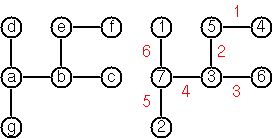
\includegraphics[scale=.2]{graphics/P92_1.png}  
% \end{figure}

Several years ago I met a mathematician who was intrigued by a problem
for which he didn't know a solution. His name was Von Koch, and I
don't know whether the problem has been solved since.

Anyway the puzzle goes like this: Given a tree with N nodes (and hence
N-1 edges). Find a way to enumerate the nodes from 1 to N and,
accordingly, the edges from 1 to N-1 in such a way, that for each edge
K the difference of its node numbers equals to
K. The conjecture is that this is always possible. 


% \begin{figure}[H]
%   \centering
% 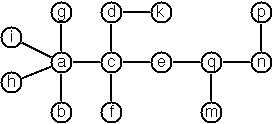
\includegraphics[scale=.6]{graphics/P92_2.png}
% \end{figure}


For small trees the problem is easy to solve by hand. However, for
larger trees, and 14 is already very large, it is extremely difficult
to find a solution. And remember, we don't know for sure whether there
is always a solution!

Write a predicate that calculates a numbering scheme for a given tree.
What is the solution for the larger tree pictured above?

\begin{wideverbatim}

We represent the tree as nested lists in the form

# edge:  number
# node:  (number . name)
# tree:  (edge node [tree ..])

For example, the representation of the first example's solution is

   (7 (7 . a)
      (4 (3 . b)
         (3 (6 . c))
         (2 (5 . e)
            (1 (4 . f)) ) )
      (6 (1 . d))
      (5 (2 . g)) )

The function 'kochConjecture' iterates a tree skeleton like

(0 (0 . a)
   (0 (0 . b)
      (0 (0 . c))
      (0 (0 . e)
         (0 (0 . f)) ) )
   (0 (0 . d))
   (0 (0 . g)) ) )

to obtain solutions like the one above.

\end{wideverbatim}

\begin{wideverbatim}


(de kochConjecture (Tree)
   (let
      (Cnt                             # Calculate number of nodes
         (recur (Tree)
            (if Tree
               (inc (sum recurse (cddr Tree)))
               0 ) )
         Edges (range 1 (dec Cnt))     # List of edge numbers
         Nodes (range 1 Cnt)           # List of node numbers
         L Nodes )
      (set Tree Cnt)                   # Set top edge (just for symmetry)
      (unless
         (recur (L)                    # Generate node number permutations
            (if (cdr L)
               (do (length L)
                  (NIL (recurse (cdr L)))
                  (rot L) )
               (use Nodes                 # Try next node number permutation
                  (recur (Tree)
                     (set (cadr Tree) (pop 'Nodes))
                     (mapc recurse (cddr Tree)) ) )
               (use Edges                 # Try to fit edges
                  (recur (Tree)
                     (let N (caadr Tree)  # Node number
                        (find
                           '((X)
                              (let E (abs (- N (caadr X)))  # Calculate edge
                                 (or
                                    (not (member E Edges))
                                    (prog
                                       (del E 'Edges)
                                       (set X E)
                                       (recurse X) ) ) ) )
                           (cddr Tree) ) ) ) ) ) )
         Tree ) ) )

\end{wideverbatim}

\begin{wideverbatim}


Test run (using 'pretty' to pretty-print the result):

(pretty
   (kochConjecture
      (0 (0 . a)
         (0 (0 . b))
         (0 (0 . c)
            (0 (0 . d)
               (0 (0 . k)) )
            (0 (0 . e)
               (0 (0 . q)
                  (0 (0 . m))
                  (0 (0 . n)
                     (0 (0 . p)) ) ) )
            (0 (0 . f)) )
         (0 (0 . g))
         (0 (0 . h))
         (0 (0 . i)) ) ) )

This returns as the first solution

(14
   (1 . a)
   (1 (2 . b))
   (13
      (14 . c)
      (11 (3 . d) (9 (12 . k)))
      (3
         (11 . e)
         (6
            (5 . q)
            (2 (7 . m))
            (5 (10 . n) (4 (6 . p))) ) )
      (10 (4 . f)) )
   (7 (8 . g))
   (8 (9 . h))
   (12 (13 . i)) )

\end{wideverbatim}

\pagebreak{}
\subsection*{{P93} (***) An arithmetic puzzle}
\label{sec:99-problems-P93}

Given a list of integer numbers, find a correct way of inserting
arithmetic signs (operators) such that the result is a correct equation.
Example: With the list of numbers (2 3 5 7 11) we can form the equations
2-3+5+7 = 11 or 2 = (3*5+7)/11 (and ten others!).

\begin{wideverbatim}

(de infix (E)
   (if (atom E)
      E
      (list
         (infix (cadr E))
         (car E)
         (infix (caddr E)) ) ) )

(de expressions (X)
   (if (cdr X)
      (mapcan
         '((I)
            (mapcan
               '((A)
                  (mapcan
                     '((B)
                        (mapcar
                           '((Op) (list Op A B))
                           '(+ - * /) ) )
                     (expressions (tail (- I) X)) ) )
               (expressions (head I X)) ) )
         (range 1 (dec (length X))) )
      (list (car X)) ) )

\end{wideverbatim}

\begin{wideverbatim}


(de equations (Lst)
   (use /
      (redef / (A B)
         (and (n0 B) (=0 (% A B)) (/ A B)) )
      (for (I 1  (> (length Lst) I)  (inc I))
         (for A (expressions (head I Lst))
            (for B (expressions (tail (- I) Lst))
               (let? N (eval A)
                  (when (= N (eval B))
                     (println (infix A) '= (infix B)) ) ) ) ) ) ) )

Test:

: (equations (2 3 5 7 11))
2 = (3 - (5 + (7 - 11)))
2 = (3 - ((5 + 7) - 11))
2 = ((3 - 5) - (7 - 11))
2 = ((3 - (5 + 7)) + 11)
2 = (((3 - 5) - 7) + 11)
2 = (((3 * 5) + 7) / 11)
(2 * (3 - 5)) = (7 - 11)
(2 - (3 - (5 + 7))) = 11
(2 - ((3 - 5) - 7)) = 11
((2 - 3) + (5 + 7)) = 11
((2 - (3 - 5)) + 7) = 11
(((2 - 3) + 5) + 7) = 11
-> NIL

\end{wideverbatim}

\pagebreak{}
\subsection*{{P95} (**) English number words}
\label{sec:99-problems-P95}

On financial documents, like cheques, numbers must sometimes be written
in full words. Example: 175 must be written as ``one hundred
seventy-five''. Write a function `fullWords' to return (non-negative)
integer numbers in full words.

\begin{wideverbatim}

(de fullWords (N)
   (cond
      ((=0 N) "zero")
      ((> 14 N)
         (get
         '("one" "two" "three" "four" "five" "six" "seven" "eight"
         "nine" "ten" "eleven" "twelve" "thirteen")
            N ) )
      ((= 15 N) "fifteen")
      ((= 18 N) "eighteen")
      ((> 20 N) (pack (fullWords (% N 10)) "teen"))
      ((> 100 N)
         (pack
            (get
               '("twen" "thir" "for" "fif" "six" "seven" "eigh" "nine")
               (dec (/ N 10)) )
            "ty"
            (unless (=0 (% N 10))
               (pack "-" (fullWords (% N 10))) ) ) )
      ((rank N '((100 . "hundred") (1000 . "thousand") (1000000 . "million")))
         (pack (fullWords (/ N (car @))) " " (cdr @) " " (fullWords (% N (car @)))) ) ) )

\end{wideverbatim}

\pagebreak{}
\subsection*{{P96} (**) Syntax checker}
\label{sec:99-problems-P96}

% \begin{figure}[H]
%   \centering
%   \includegraphics[scale=.6]{graphics/P96_1.png}
% \end{figure}

In a certain programming language (Ada) identifiers are defined by the
syntax diagram (railroad chart) opposite. Transform the syntax diagram
into a system of syntax gndiagrams which do not contain loops; i.e.
which are purely recursive. Using these modified diagrams, write a
function `identifier' that can check whether or not a given string is
a legal identifier.

\begin{wideverbatim}

(de identifier (Str)
   (and
      (>= "z" (lowc (car (setq Str (chop Str)))) "a")
      (not
         (find
            '((C)
               (nor
                  (= "_" C)
                  (>= "9" C "0")
                  (>= "z" (lowc C) "a") ) )
            (cdr Str) ) ) ) )

\end{wideverbatim}


\pagebreak{}
\subsection*{{P97} (**) Sudoku}
\label{sec:99-problems-P97}

Sudoku puzzles go like this:

\begin{wideverbatim}
Problem statement                 Solution

 .  .  4 | 8  .  . | .  1  7      9  3  4 | 8  2  5 | 6  1  7
         |         |                      |         |
 6  7  . | 9  .  . | .  .  .      6  7  2 | 9  1  4 | 8  5  3
         |         |                      |         |
 5  .  8 | .  3  . | .  .  4      5  1  8 | 6  3  7 | 9  2  4
 --------+---------+--------      --------+---------+--------
 3  .  . | 7  4  . | 1  .  .      3  2  5 | 7  4  8 | 1  6  9
         |         |                      |         |
 .  6  9 | .  .  . | 7  8  .      4  6  9 | 1  5  3 | 7  8  2
         |         |                      |         |
 .  .  1 | .  6  9 | .  .  5      7  8  1 | 2  6  9 | 4  3  5
 --------+---------+--------      --------+---------+--------
 1  .  . | .  8  . | 3  .  6      1  9  7 | 5  8  2 | 3  4  6
         |         |                      |         |
 .  .  . | .  .  6 | .  9  1      8  5  3 | 4  7  6 | 2  9  1
         |         |                      |         |
 2  4  . | .  .  1 | 5  .  .      2  4  6 | 3  9  1 | 5  7  8
\end{wideverbatim}

Every spot in the puzzle belongs to a (horizontal) row and a (vertical)
column, as well as to one single 3x3 square (which we call ``square''
for short). At the beginning, some of the spots carry a single-digit
number between 1 and 9. The problem is to fill the missing spots with
digits in such a way that every number between 1 and 9 appears exactly
once in each row, in each column, and in each square.

\begin{wideverbatim}

(load "@lib/simul.l")

### Fields/Board ###
# val lst

(setq
   *Board (grid 9 9)
   *Fields (apply append *Board) )

# Init values to zero (empty)
(for L *Board
   (for This L
      (=: val 0) ) )

# Build lookup lists
(for (X . L) *Board
   (for (Y . This) L
      (=: lst
         (make
            (let A (* 3 (/ (dec X) 3))
               (do 3
                  (inc 'A)
                  (let B (* 3 (/ (dec Y) 3))
                     (do 3
                        (inc 'B)
                        (unless (and (= A X) (= B Y))
                           (link
                              (prop (get *Board A B) 'val) ) ) ) ) ) )
            (for Dir '(`west `east `south `north)
               (for (This (Dir This)  This  (Dir This))
                  (unless (memq (:: val) (made))
                     (link (:: val)) ) ) ) ) ) ) )

# Cut connections (for display only)
(for (X . L) *Board
   (for (Y . This) L
      (when (member X (3 6))
         (con (car (val This))) )
      (when (member Y (4 7))
         (set (cdr (val This))) ) ) )


\end{wideverbatim}

\begin{wideverbatim}

# Display board
(de display ()
   (disp *Board 0
      '((This)
         (if (=0 (: val))
            "   "
            (pack " " (: val) " ") ) ) ) )

# Initialize board
(de main (Lst)
   (for (Y . L) Lst
      (for (X . N) L
         (put *Board X (- 10 Y) 'val N) ) )
   (display) )

# Find solution
(de go ()
   (unless
      (recur (*Fields)
         (with (car *Fields)
            (if (=0 (: val))
               (loop
                  (NIL
                     (or
                        (assoc (inc (:: val)) (: lst))
                        (recurse (cdr *Fields)) ) )
                  (T (= 9 (: val)) (=: val 0)) )
               (recurse (cdr *Fields)) ) ) )
      (display) ) )


\end{wideverbatim}

\begin{wideverbatim}

### Usage ###
: (main
   (quote
      (0 0 4 8 0 0 0 1 7)
      (6 7 0 9 0 0 0 0 0)
      (5 0 8 0 3 0 0 0 4)
      (3 0 0 7 4 0 1 0 0)
      (0 6 9 0 0 0 7 8 0)
      (0 0 1 0 6 9 0 0 5)
      (1 0 0 0 8 0 3 0 6)
      (0 0 0 0 0 6 0 9 1)
      (2 4 0 0 0 1 5 0 0) ) )
   +---+---+---+---+---+---+---+---+---+
 9 |         4 | 8         |     1   7 |
   +   +   +   +   +   +   +   +   +   +
 8 | 6   7     | 9         |           |
   +   +   +   +   +   +   +   +   +   +
 7 | 5       8 |     3     |         4 |
   +---+---+---+---+---+---+---+---+---+
 6 | 3         | 7   4     | 1         |
   +   +   +   +   +   +   +   +   +   +
 5 |     6   9 |           | 7   8     |
   +   +   +   +   +   +   +   +   +   +
 4 |         1 |     6   9 |         5 |
   +---+---+---+---+---+---+---+---+---+
 3 | 1         |     8     | 3       6 |
   +   +   +   +   +   +   +   +   +   +
 2 |           |         6 |     9   1 |
   +   +   +   +   +   +   +   +   +   +
 1 | 2   4     |         1 | 5         |
   +---+---+---+---+---+---+---+---+---+
     a   b   c   d   e   f   g   h   i
-> NIL


\end{wideverbatim}

\begin{wideverbatim}


: (go)
   +---+---+---+---+---+---+---+---+---+
 9 | 9   3   4 | 8   2   5 | 6   1   7 |
   +   +   +   +   +   +   +   +   +   +
 8 | 6   7   2 | 9   1   4 | 8   5   3 |
   +   +   +   +   +   +   +   +   +   +
 7 | 5   1   8 | 6   3   7 | 9   2   4 |
   +---+---+---+---+---+---+---+---+---+
 6 | 3   2   5 | 7   4   8 | 1   6   9 |
   +   +   +   +   +   +   +   +   +   +
 5 | 4   6   9 | 1   5   3 | 7   8   2 |
   +   +   +   +   +   +   +   +   +   +
 4 | 7   8   1 | 2   6   9 | 4   3   5 |
   +---+---+---+---+---+---+---+---+---+
 3 | 1   9   7 | 5   8   2 | 3   4   6 |
   +   +   +   +   +   +   +   +   +   +
 2 | 8   5   3 | 4   7   6 | 2   9   1 |
   +   +   +   +   +   +   +   +   +   +
 1 | 2   4   6 | 3   9   1 | 5   7   8 |
   +---+---+---+---+---+---+---+---+---+
     a   b   c   d   e   f   g   h   i
-> NIL

\end{wideverbatim}

\pagebreak{}
\subsection*{{P98} (***) Nonograms}
\label{sec:99-problems-P98}

Around 1994, a certain kind of puzzles was very popular in England. The
``Sunday Telegraph'' newspaper wrote: ``Nonograms are puzzles from Japan
and are currently published each week only in The Sunday Telegraph.
Simply use your logic and skill to complete the grid and reveal a
picture or diagram.'' As a PicoLisp programmer, you are in a better
situation: you can have your computer do the work! Just write a little
program ;-).

 The puzzle goes like this: Essentially, each row and
column of a rectangular bitmap is annotated with the respective lengths
of its distinct strings of occupied cells. The person who solves the
puzzle must complete the bitmap given only these lengths.

\begin{wideverbatim}
   Problem statement:          Solution:

   |_|_|_|_|_|_|_|_| 3         |_|X|X|X|_|_|_|_| 3
   |_|_|_|_|_|_|_|_| 2 1       |X|X|_|X|_|_|_|_| 2 1
   |_|_|_|_|_|_|_|_| 3 2       |_|X|X|X|_|_|X|X| 3 2
   |_|_|_|_|_|_|_|_| 2 2       |_|_|X|X|_|_|X|X| 2 2
   |_|_|_|_|_|_|_|_| 6         |_|_|X|X|X|X|X|X| 6
   |_|_|_|_|_|_|_|_| 1 5       |X|_|X|X|X|X|X|_| 1 5
   |_|_|_|_|_|_|_|_| 6         |X|X|X|X|X|X|_|_| 6
   |_|_|_|_|_|_|_|_| 1         |_|_|_|_|X|_|_|_| 1
   |_|_|_|_|_|_|_|_| 2         |_|_|_|X|X|_|_|_| 2
   1 3 1 7 5 3 4 3             1 3 1 7 5 3 4 3
   2 1 5 1                     2 1 5 1
\end{wideverbatim}             

For the example above, the problem can be stated as the two lists ((3)
(2 1) (3 2) (2 2) (6) (1 5) (6) (1) (2)) and ((1 2) (3 1) (1 5) (7 1)
(5) (3) (4) (3)) which give the ``solid'' lengths of the rows and
columns, top-to-bottom and left-to-right, respectively. Published
puzzles are larger than this example, e.g. 25 x 20, and apparently
always have unique solutions.


\begin{wideverbatim}

(de nonogram (LstX LstY)
   (let Lim (** 2 (length LstY))
      (_nonogX LstX) ) )

(de _nonogX (LstX Res)
   (if LstX
      (_nonogY LstX Res)
      (when
         (= LstY
            (make
               (for (I Lim (gt0 (setq I (>> 1 I))))
                  (link
                     (flip
                        (make
                           (let C NIL
                              (for N Res
                                 (if2 (bit? I N) C
                                    (inc 'C)
                                    (one C)
                                    (prog (link C) (off C)) ) )
                              (and C (link @)) ) ) ) ) ) ) )
         (for N (flip Res)
            (for (I Lim (gt0 (setq I (>> 1 I))))
               (prin "|" (if (bit? I N) "X" "_")) )
            (prinl "|") ) ) ) )


\end{wideverbatim}

\begin{wideverbatim}


(de _nonogY (LstX Res)
   (let (Lst (mapcar '((N) (cons 1 (** 2 N))) (car LstX))  P Lst)
      (recur (P)
         (ifn P
            (let N 0
               (for X Lst
                  (setq N
                     (+
                        (* 2 N (car X) (cdr X))
                        (* (car X) (dec (cdr X))) ) ) )
               (when (> Lim N)
                  (_nonogX (cdr LstX) (cons N Res))
                  T ) )
            (prog1 (recurse (cdr P))
               (while
                  (prog
                     (set (car P) (* 2 (caar P)))
                     (recurse (cdr P)) ) )
               (set (car P) 1) ) ) ) ) )

: (nonogram
   '((3) (2 1) (3 2) (2 2) (6) (1 5) (6) (1) (2))
   '((1 2) (3 1) (1 5) (7 1) (5) (3) (4) (3)) )
|_|X|X|X|_|_|_|_|
|X|X|_|X|_|_|_|_|
|_|X|X|X|_|_|X|X|
|_|_|X|X|_|_|X|X|
|_|_|X|X|X|X|X|X|
|X|_|X|X|X|X|X|_|
|X|X|X|X|X|X|_|_|
|_|_|_|_|X|_|_|_|
|_|_|_|X|X|_|_|_|
-> T

\end{wideverbatim}

\pagebreak{}
\subsection*{{P99} (***) Crossword puzzle}
\label{sec:99-problems-P99}

Given an empty (or almost empty) framework of a crossword puzzle and a
set of words. The problem is to place the words into the framework.

% \begin{figure}[H]
%   \centering
%    \includegraphics[scale=.6]{graphics/P99_1.png}  
% \end{figure}

The particular crossword puzzle is specified in a text file which
first lists the words (one word per line) in an arbitrary order. Then,
after an empty line, the crossword framework is defined. In this
framework specification, an empty character location is represented by
a dot (.). In order to make the solution easier, character locations
can also contain predefined character values. The puzzle opposite is
defined in the file \href{!wiki?99p99a}{p99a.dat}, other examples are
\href{!wiki?99p99b}{p99b.dat} and \href{!wiki?99p99d}{p99d.dat}. There
is also an example of a puzzle (\href{!wiki?99p99c}{p99c.dat}) which
does not have a solution.

\emph{Words} are strings (character lists) of at least two characters.
A horizontal or vertical sequence of character places in the crossword
puzzle framework is called a \emph{site}.

Our problem is to find a compatible way of placing words onto sites.

\begin{wideverbatim}

(load "@lib/simul.l")

(de crossword (File)
   (use (Words Data Grid Slots Org)
      (in File
         (setq
            Words (flip (by length sort (make (while (line) (link (trim @))))))
            Data (flip (make (while (line) (link (trim @)))))   # Read data
            Len (apply max (mapcar length Data))
            Grid (grid Len (length Data)) ) )            # Create grid
      (for Col Grid  # Set initial data
         (use Data
            (for This Col
               (let C (pop Data)
                  (=: char (unless (sp? C) C)) )
               (pop 'Data) ) ) )
      (setq Slots
         (mapcar
            '((L) (cons (length (car L)) L))
            (by length group
               (make
                  (for Col Grid  # Init slots
                     (for This Col
                        (when (: char)
                           (and  # Check horizontal slot
                              (not (; (west This) char))
                              (; (east This) char)
                              (; (east (east This)) char)
                              (link
                                 (make
                                    (for (This This (: char) (east This))
                                       (link This) ) ) ) )
                           (and  # Check vertical slot
                              (not (; (north This) char))
                              (; (south This) char)
                              (; (south (south This)) char)
                              (link
                                 (make
                                    (for (This This (: char) (south This))
                                       (link This) ) ) ) ) ) ) ) ) ) ) )

\end{wideverbatim}

\begin{wideverbatim}


      (recur (Words)
         (if Words
            (for Slot (cdr (assoc (length (car Words)) Slots))
               (unless
                  (find
                     '((This C) (nor (= C (: char)) (= "." (: char))))
                     Slot
                     (car Words) )
                  (let Org (mapcar get Slot '(char .))
                     (mapc put Slot '(char .) (car Words))
                     (recurse (cdr Words))
                     (mapc put Slot '(char .) Org) ) ) )
            (disp Grid T  # Found a solution: Display it
               '((This)
                  (if (: char)
                     (pack " " @ " ")
                     "###" ) ) ) ) ) ) )

: (crossword "p99a.dat")

   +---+---+---+---+---+---+---+---+---+
 6 | P | R | O | L | O | G |###|###| E |
   +---+---+---+---+---+---+---+---+---+
 5 | E |###| N |###|###| N |###|###| M |
   +---+---+---+---+---+---+---+---+---+
 4 | R |###| L | I | N | U | X |###| A |
   +---+---+---+---+---+---+---+---+---+
 3 | L |###| I |###| F |###| M | A | C |
   +---+---+---+---+---+---+---+---+---+
 2 |###|###| N |###| S | Q | L |###| S |
   +---+---+---+---+---+---+---+---+---+
 1 |###| W | E | B |###|###|###|###|###|
   +---+---+---+---+---+---+---+---+---+
     a   b   c   d   e   f   g   h   i

\end{wideverbatim}


\pagebreak{}
 \textbf{Hints:}

 (1) The problem is not easy. You will need some time to thoroughly
 understand it. So, don't give up too early! And remember that the
 objective is a clean solution, not just a quick-and-dirty hack!

 (2) Reading the data file is a tricky problem (in Prolog?).

 (3) For efficiency reasons it is important, at least for larger
 puzzles, to sort the words and the sites in a particular order. For
 this part of the problem, the solution of P28 may be very helpful.


%%%%%%%%%%%%%%%%%%%%%part.tex%%%%%%%%%%%%%%%%%%%%%%%%%%%%%%%%%%
% 
% sample part title
%
% Use this file as a template for your own input.
%
%%%%%%%%%%%%%%%%%%%%%%%% Springer %%%%%%%%%%%%%%%%%%%%%%%%%%

\begin{partbacktext}
\part{Rosetta Code}
\noindent Rosetta Code
(\href{http://rosettacode.org/wiki/Rosetta_Code}{rosettacode.org})
is a programming chrestomathy site. The idea is to present solutions
to the same task in as many different languages as possible, to
demonstrate how languages are similar and different, and to aid a
person with a grounding in one approach to a problem in learning
another. Rosetta Code currently\footnote{accessed online 21-08-2012}
has 600 tasks, 97 draft tasks, and is aware of 471 languages.
\end{partbacktext}

%%%%%%%%%%%%%%%%%%%%% chapter.tex %%%%%%%%%%%%%%%%%%%%%%%%%%%%%%%%%
%
% sample chapter
%
% Use this file as a template for your own input.
%
%%%%%%%%%%%%%%%%%%%%%%%% Springer-Verlag %%%%%%%%%%%%%%%%%%%%%%%%%%
%\motto{Use the template \emph{chapter.tex} to style the various elements of your chapter content.}

\chapter{Rosetta Code Tasks starting with Numbers}
\label{rosettacode-numbers}

\section*{100 doors}

Problem: You have 100 doors in a row that are all initially closed.
You make 100 passes by the doors. The first time through, you visit
every door and toggle the door (if the door is closed, you open it; if
it is open, you close it). The second time you only visit every 2nd
door (door \#2, \#4, \#6, \ldots{}). The third time, every 3rd door
(door \#3, \#6, \#9, \ldots{}), etc, until you only visit the 100th
door.

Question: What state are the doors in after the last pass? Which are
open, which are closed?

\textbf{Alternate:} As noted in this page's discussion page, the only
doors that remain open are whose numbers are perfect squares of
integers. Opening only those doors is an optimization that may also be
expressed.

\begin{wideverbatim}
unoptimized

(let Doors (need 100)
   (for I 100
      (for (D (nth Doors I)  D  (cdr (nth D I)))
         (set D (not (car D))) ) )
   (println Doors) )

optimized

(let Doors (need 100)
   (for I (sqrt 100)
      (set (nth Doors (* I I)) T) )
   (println Doors) )
\end{wideverbatim}

\pagebreak{}
\section*{24 game}

The 24 Game tests one's mental arithmetic.

Write a program that randomly chooses and displays four digits, each
from one to nine, with repetitions allowed. The program should prompt
for the player to enter an equation using \emph{just} those, and
\emph{all} of those four digits. The program should \emph{check} then
evaluate the expression. The goal is for the player to enter an
expression that evaluates to \textbf{24}.

\begin{itemize}
\item
  Only multiplication, division, addition, and subtraction
  operators/functions are allowed.
\item
  Division should use floating point or rational arithmetic, etc, to
  preserve remainders.
\item
  Brackets are allowed, if using an infix expression evaluator.
\item
  Forming multiple digit numbers from the supplied digits is
  \emph{disallowed}. (So an answer of 12+12 when given 1, 2, 2, and 1 is
  wrong).
\item
  The order of the digits when given does not have to be preserved.
\end{itemize}

Note:

\begin{itemize}
\item The type of expression evaluator used is not mandated. An RPN
  evaluator is equally acceptable for example.
\item
  The task is not for the program to generate the expression, or test
  whether an expression is even possible.
\end{itemize}

C.f: 24 game Player

\textbf{Reference}

\begin{enumerate}
\item
  \href{http://www.bbc.co.uk/dna/h2g2/A933121}{The 24 Game} on h2g2.
\end{enumerate}


\begin{wideverbatim}

(de checkExpression (Lst Exe)
   (make
      (when (diff Lst (fish num? Exe))
         (link "Not all numbers used" ) )
      (when (diff (fish num? Exe) Lst)
         (link "Using wrong number(s)") )
      (when (diff (fish sym? Exe) '(+ - * /))
         (link "Using illegal operator(s)") ) ) )

(loop
   (setq Numbers (make (do 4 (link (rand 1 9)))))
   (prinl
      "Please enter a Lisp expression using (, ), +, -, *, / and "
      (glue ", " Numbers) )
   (prin "Or a single dot '.' to stop: ")
   (T (= "." (setq Reply (catch '(NIL) (in NIL (read)))))
      (bye) )
   (cond
      ((str? Reply)
         (prinl "-- Input error: " Reply) )
      ((checkExpression Numbers Reply)
         (prinl "-- Illegal Expression")
         (for S @
            (space 3)
            (prinl S) ) )
      ((str? (setq Result (catch '(NIL) (eval Reply))))
         (prinl "-- Evaluation error: " @) )
      ((= 24 Result)
         (prinl "++ Congratulations! Correct result :-)") )
      (T (prinl "Sorry, this gives " Result)) )
   (prinl) )

\end{wideverbatim}

\begin{wideverbatim}

Output:

Please enter a Lisp expression using (, ), +, -, *, / and 1, 3, 3, 5
Or a single dot '.' to stop: (* (+ 3 1) (+ 5 1))
++ Congratulations! Correct result :-)

Please enter a Lisp expression using (, ), +, -, *, / and 8, 4, 7, 1
Or a single dot '.' to stop: (* 8 (\% 7 3) 9)
-- Illegal Expression
   Not all numbers used
   Using wrong number(s)
   Using illegal operator(s)

Please enter a Lisp expression using (, ), +, -, *, / and 4, 2, 2, 3
Or a single dot '.' to stop: (/ (+ 4 3) (- 2 2))
-- Evaluation error: Div/0

Please enter a Lisp expression using (, ), +, -, *, / and 8, 4, 5, 9
Or a single dot '.' to stop: .

\end{wideverbatim}

\pagebreak{}
\section*{24 game/Solve}


Write a function that given four digits subject to the rules of the
24 game, computes an expression to solve the game
if possible.

Show examples of solutions generated by the function

C.F: Arithmetic Evaluator


\begin{wideverbatim}

We use Pilog (PicoLisp Prolog) to solve this task

(be play24 (@Lst @Expr)                # Define Pilog rule
   (permute @Lst (@A @B @C @D))
   (member @Op1 (+ - * /))
   (member @Op2 (+ - * /))
   (member @Op3 (+ - * /))
   (or
      ((equal @Expr (@Op1 (@Op2 @A @B) (@Op3 @C @D))))
      ((equal @Expr (@Op1 @A (@Op2 @B (@Op3 @C @D))))) )
   (@ = 24 (catch '("Div/0") (eval (-> @Expr)))) )

(de play24 (A B C D)                   # Define PicoLisp function
   (pilog
      (quote
         @L (list A B C D)
         (play24 @L @X) )
      (println @X) ) )

(play24 5 6 7 8)                       # Call 'play24' function

Output:

(* (+ 5 7) (- 8 6))
(* 6 (+ 5 (- 7 8)))
(* 6 (- 5 (- 8 7)))
(* 6 (- 5 (/ 8 7)))
(* 6 (+ 7 (- 5 8)))
(* 6 (- 7 (- 8 5)))
(* 6 (/ 8 (- 7 5)))
(/ (* 6 8) (- 7 5))
(* (+ 7 5) (- 8 6))
(* (- 8 6) (+ 5 7))
(* (- 8 6) (+ 7 5))
(* 8 (/ 6 (- 7 5)))
(/ (* 8 6) (- 7 5))

\end{wideverbatim}

\pagebreak{}
\section*{99 Bottles of Beer}


In this puzzle, write code to print out the entire ``99 bottles of beer
on the wall'' song. For those who do not know the song, the lyrics
follow this form:

\begin{verbatim}
X bottles of beer on the wall
X bottles of beer
Take one down, pass it around
X-1 bottles of beer on the wall

X-1 bottles of beer on the wall
...
Take one down, pass it around
0 bottles of beer on the wall
\end{verbatim}

Where X and X-1 are replaced by numbers of course. Grammatical support
for ``1 bottle of beer'' is optional. As with any puzzle, try to do it
in as creative/concise/comical a way as possible (simple, obvious
solutions allowed, too).

See also:
\href{http://99-bottles-of-beer.net/}{http://99-bottles-of-beer.net/}


\begin{wideverbatim}

(de bottles (N)
   (case N
      (0 "No more beer")
      (1 "One bottle of beer")
      (T (cons N " bottles of beer")) ) )

(for (N 99 (gt0 N))
   (prinl (bottles N) " on the wall,")
   (prinl (bottles N) ".")
   (prinl "Take one down, pass it around,")
   (prinl (bottles (dec 'N)) " on the wall.")
   (prinl) )

\end{wideverbatim}




% %%%%%%%%%%%%%%%%%%%%%%%% referenc.tex %%%%%%%%%%%%%%%%%%%%%%%%%%%%%%
% sample references
% %
% Use this file as a template for your own input.
%
%%%%%%%%%%%%%%%%%%%%%%%% Springer-Verlag %%%%%%%%%%%%%%%%%%%%%%%%%%
%
% BibTeX users please use
% \bibliographystyle{}
% \bibliography{}
%
\biblstarthook{In view of the parallel print and (chapter-wise) online publication of your book at \url{www.springerlink.com} it has been decided that -- as a genreral rule --  references should be sorted chapter-wise and placed at the end of the individual chapters. However, upon agreement with your contact at Springer you may list your references in a single seperate chapter at the end of your book. Deactivate the class option \texttt{sectrefs} and the \texttt{thebibliography} environment will be put out as a chapter of its own.\\\indent
References may be \textit{cited} in the text either by number (preferred) or by author/year.\footnote{Make sure that all references from the list are cited in the text. Those not cited should be moved to a separate \textit{Further Reading} section or chapter.} The reference list should ideally be \textit{sorted} in alphabetical order -- even if reference numbers are used for the their citation in the text. If there are several works by the same author, the following order should be used: 
\begin{enumerate}
\item all works by the author alone, ordered chronologically by year of publication
\item all works by the author with a coauthor, ordered alphabetically by coauthor
\item all works by the author with several coauthors, ordered chronologically by year of publication.
\end{enumerate}
The \textit{styling} of references\footnote{Always use the standard abbreviation of a journal's name according to the ISSN \textit{List of Title Word Abbreviations}, see \url{http://www.issn.org/en/node/344}} depends on the subject of your book:
\begin{itemize}
\item The \textit{two} recommended styles for references in books on \textit{mathematical, physical, statistical and computer sciences} are depicted in ~\cite{science-contrib, science-online, science-mono, science-journal, science-DOI} and ~\cite{phys-online, phys-mono, phys-journal, phys-DOI, phys-contrib}.
\item Examples of the most commonly used reference style in books on \textit{Psychology, Social Sciences} are~\cite{psysoc-mono, psysoc-online,psysoc-journal, psysoc-contrib, psysoc-DOI}.
\item Examples for references in books on \textit{Humanities, Linguistics, Philosophy} are~\cite{humlinphil-journal, humlinphil-contrib, humlinphil-mono, humlinphil-online, humlinphil-DOI}.
\item Examples of the basic Springer style used in publications on a wide range of subjects such as \textit{Computer Science, Economics, Engineering, Geosciences, Life Sciences, Medicine, Biomedicine} are ~\cite{basic-contrib, basic-online, basic-journal, basic-DOI, basic-mono}. 
\end{itemize}
}

\begin{thebibliography}{99.}%
% and use \bibitem to create references.
%
% Use the following syntax and markup for your references if 
% the subject of your book is from the field 
% "Mathematics, Physics, Statistics, Computer Science"
%
% Contribution 
\bibitem{science-contrib} Broy, M.: Software engineering --- from auxiliary to key technologies. In: Broy, M., Dener, E. (eds.) Software Pioneers, pp. 10-13. Springer, Heidelberg (2002)
%
% Online Document
\bibitem{science-online} Dod, J.: Effective substances. In: The Dictionary of Substances and Their Effects. Royal Society of Chemistry (1999) Available via DIALOG. \\
\url{http://www.rsc.org/dose/title of subordinate document. Cited 15 Jan 1999}
%
% Monograph
\bibitem{science-mono} Geddes, K.O., Czapor, S.R., Labahn, G.: Algorithms for Computer Algebra. Kluwer, Boston (1992) 
%
% Journal article
\bibitem{science-journal} Hamburger, C.: Quasimonotonicity, regularity and duality for nonlinear systems of partial differential equations. Ann. Mat. Pura. Appl. \textbf{169}, 321--354 (1995)
%
% Journal article by DOI
\bibitem{science-DOI} Slifka, M.K., Whitton, J.L.: Clinical implications of dysregulated cytokine production. J. Mol. Med. (2000) doi: 10.1007/s001090000086 
%
\bigskip

% Use the following (APS) syntax and markup for your references if 
% the subject of your book is from the field 
% "Mathematics, Physics, Statistics, Computer Science"
%
% Online Document
\bibitem{phys-online} J. Dod, in \textit{The Dictionary of Substances and Their Effects}, Royal Society of Chemistry. (Available via DIALOG, 1999), 
\url{http://www.rsc.org/dose/title of subordinate document. Cited 15 Jan 1999}
%
% Monograph
\bibitem{phys-mono} H. Ibach, H. L\"uth, \textit{Solid-State Physics}, 2nd edn. (Springer, New York, 1996), pp. 45-56 
%
% Journal article
\bibitem{phys-journal} S. Preuss, A. Demchuk Jr., M. Stuke, Appl. Phys. A \textbf{61}
%
% Journal article by DOI
\bibitem{phys-DOI} M.K. Slifka, J.L. Whitton, J. Mol. Med., doi: 10.1007/s001090000086
%
% Contribution 
\bibitem{phys-contrib} S.E. Smith, in \textit{Neuromuscular Junction}, ed. by E. Zaimis. Handbook of Experimental Pharmacology, vol 42 (Springer, Heidelberg, 1976), p. 593
%
\bigskip
%
% Use the following syntax and markup for your references if 
% the subject of your book is from the field 
% "Psychology, Social Sciences"
%
%
% Monograph
\bibitem{psysoc-mono} Calfee, R.~C., \& Valencia, R.~R. (1991). \textit{APA guide to preparing manuscripts for journal publication.} Washington, DC: American Psychological Association.
%
% Online Document
\bibitem{psysoc-online} Dod, J. (1999). Effective substances. In: The dictionary of substances and their effects. Royal Society of Chemistry. Available via DIALOG. \\
\url{http://www.rsc.org/dose/Effective substances.} Cited 15 Jan 1999.
%
% Journal article
\bibitem{psysoc-journal} Harris, M., Karper, E., Stacks, G., Hoffman, D., DeNiro, R., Cruz, P., et al. (2001). Writing labs and the Hollywood connection. \textit{J Film} Writing, 44(3), 213--245.
%
% Contribution 
\bibitem{psysoc-contrib} O'Neil, J.~M., \& Egan, J. (1992). Men's and women's gender role journeys: Metaphor for healing, transition, and transformation. In B.~R. Wainrig (Ed.), \textit{Gender issues across the life cycle} (pp. 107--123). New York: Springer.
%
% Journal article by DOI
\bibitem{psysoc-DOI}Kreger, M., Brindis, C.D., Manuel, D.M., Sassoubre, L. (2007). Lessons learned in systems change initiatives: benchmarks and indicators. \textit{American Journal of Community Psychology}, doi: 10.1007/s10464-007-9108-14.
%
%
% Use the following syntax and markup for your references if 
% the subject of your book is from the field 
% "Humanities, Linguistics, Philosophy"
%
\bigskip
%
% Journal article
\bibitem{humlinphil-journal} Alber John, Daniel C. O'Connell, and Sabine Kowal. 2002. Personal perspective in TV interviews. \textit{Pragmatics} 12:257--271
%
% Contribution 
\bibitem{humlinphil-contrib} Cameron, Deborah. 1997. Theoretical debates in feminist linguistics: Questions of sex and gender. In \textit{Gender and discourse}, ed. Ruth Wodak, 99--119. London: Sage Publications.
%
% Monograph
\bibitem{humlinphil-mono} Cameron, Deborah. 1985. \textit{Feminism and linguistic theory.} New York: St. Martin's Press.
%
% Online Document
\bibitem{humlinphil-online} Dod, Jake. 1999. Effective substances. In: The dictionary of substances and their effects. Royal Society of Chemistry. Available via DIALOG. \\
http://www.rsc.org/dose/title of subordinate document. Cited 15 Jan 1999
%
% Journal article by DOI
\bibitem{humlinphil-DOI} Suleiman, Camelia, Daniel C. O�Connell, and Sabine Kowal. 2002. `If you and I, if we, in this later day, lose that sacred fire...�': Perspective in political interviews. \textit{Journal of Psycholinguistic Research}. doi: 10.1023/A:1015592129296.
%
%
%
\bigskip
%
%
% Use the following syntax and markup for your references if 
% the subject of your book is from the field 
% "Computer Science, Economics, Engineering, Geosciences, Life Sciences"
%
%
% Contribution 
\bibitem{basic-contrib} Brown B, Aaron M (2001) The politics of nature. In: Smith J (ed) The rise of modern genomics, 3rd edn. Wiley, New York 
%
% Online Document
\bibitem{basic-online} Dod J (1999) Effective Substances. In: The dictionary of substances and their effects. Royal Society of Chemistry. Available via DIALOG. \\
\url{http://www.rsc.org/dose/title of subordinate document. Cited 15 Jan 1999}
%
% Journal article by DOI
\bibitem{basic-DOI} Slifka MK, Whitton JL (2000) Clinical implications of dysregulated cytokine production. J Mol Med, doi: 10.1007/s001090000086
%
% Journal article
\bibitem{basic-journal} Smith J, Jones M Jr, Houghton L et al (1999) Future of health insurance. N Engl J Med 965:325--329
%
% Monograph
\bibitem{basic-mono} South J, Blass B (2001) The future of modern genomics. Blackwell, London 
%
\end{thebibliography}


%%%%%%%%%%%%%%%%%%%%% chapter.tex %%%%%%%%%%%%%%%%%%%%%%%%%%%%%%%%%
%
% sample chapter
%
% Use this file as a template for your own input.
%
%%%%%%%%%%%%%%%%%%%%%%%% Springer-Verlag %%%%%%%%%%%%%%%%%%%%%%%%%%
%\motto{Use the template \emph{chapter.tex} to style the various elements of your chapter content.}

\chapter{Rosetta Code Tasks starting with A}
\label{rosettacode-numbers}

\section*{A+B}

\textbf{A+B} - in programming contests, classic problem, which is given
so contestants can gain familiarity with online judging system being
used.

\textbf{Problem statement:} Given 2 integer numbers, A and B. One
needs to find their sum.

\textbf{Input data:} Two integer numbers are written in the input
stream, separated by space.

\begin{figure}[H]
\centering
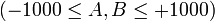
\includegraphics[scale=.6]{graphics/a344abb2a9a00cb2de6679a485115ce3.png}
% \caption{(-1000 \textbackslash{}le A,B \textbackslash{}le +1000)}
\end{figure}

\textbf{Output data:} The required output is one integer: the sum of A
and B.

\textbf{Example:}

\ctable[pos = H, center, botcap]{lc}{% notes
}{% rows
\FL
 Input & Output 
\ML
\texttt{2 2} & \texttt{4} 
\NN
\texttt{3 2} & \texttt{5} 
\LL
}

% \noalign{\medskip}


\begin{wideverbatim}

(+ (read) (read))
3 4
-> 7

\end{wideverbatim}

\pagebreak{}
\section*{Abstract type}

\textbf{Abstract type} is a type without instances or without
definition.

For example in object-oriented programming using some languages,
abstract types can be partial implementations of other types, which
are to be derived there-from. An abstract type may provide
implementation of some operations and/or components. Abstract types
without any implementation are called \textbf{interfaces}. In the
languages that do not support multiple inheritance (Ada, Java),
classes can, nonetheless, inherit from multiple interfaces. The
languages with multiple inheritance (like C++) usually make no
distinction between partially implementable abstract types and
interfaces. Because the abstract type's implementation is incomplete,
OO languages normally prevent instantiation from them (instantiation
must derived from one of their descendant classes).

The term \textbf{abstract datatype} also may denote a type, with an
implementation provided by the programmer rather than directly by the
language (a \textbf{built-in} or an inferred type). Here the word
\emph{abstract} means that the implementation is abstracted away,
irrelevant for the user of the type. Such implementation can and
should be hidden if the language supports separation of implementation
and specification. This hides complexity while allowing the
implementation to change without repercussions on the usage. The
corresponding software design practice is said to follow the
information hiding principle.

It is important not to confuse this \emph{abstractness} (of
implementation) with one of the \textbf{abstract type}. The latter is
abstract in the sense that the set of its values is empty. In the sense
of implementation abstracted away, all user-defined types are abstract.

In some languages, like for example in Objective Caml which is strongly
statically typed, it is also possible to have \textbf{abstract types}
that are not OO related and are not an abstractness too. These are
\emph{pure abstract types} without any definition even in the
implementation and can be used for example for the type algebra, or for
some consistence of the type inference. For example in this area, an
abstract type can be used as a phantom type to augment another type as
its parameter.

\textbf{Task}: show how an abstract type can be declared in the
language. If the language makes a distinction between interfaces and
partially implemented types illustrate both.


\begin{wideverbatim}

# In PicoLisp there is no formal difference between abstract and concrete
# classes, just a naming convention where abstract classes start with a
# lower case character after the '+' (the naming convention for classes).
# This tells the programmer that this class has not sufficient methods
# defined to survive on its own.

(class +abstractClass)

(dm someMethod> ()
   (foo)
   (bar) )

\end{wideverbatim}

\pagebreak{}
\section*{Accumulator factory}


A problem posed by Paul Graham is that of creating a function that
takes a single (numeric) argument and which returns another function
that is an accumulator. The returned accumulator function in turn also
takes a single numeric argument, and returns the sum of all the
numeric values passed in so far to that accumulator (including the
initial value passed when the accumulator was created).

The detailed rules are at
\href{http://paulgraham.com/accgensub.html}{http://paulgraham.com/accgensub.html}
and are reproduced here for simplicity (with additions in \emph{small
  italic text}).

Before you submit an example, make sure the function

\begin{enumerate}
\item
  Takes a number n and returns a function (lets call it g), that takes a
  number i, and returns n incremented by the accumulation of i from
  every call of function g(i).\\Although these exact function and
  parameter names need not be used
\item
  Works for any numeric type-- i.e. can take both ints and floats and
  returns functions that can take both ints and floats. (It is not
  enough simply to convert all input to floats. An accumulator that has
  only seen integers must return integers.) \emph{(i.e., if the language
  doesn't allow for numeric polymorphism, you have to use overloading or
  something like that)}
\item
  Generates functions that return the sum of every number ever passed to
  them, not just the most recent. \emph{(This requires a piece of state
  to hold the accumulated value, which in turn means that pure
  functional languages can't be used for this task.)}
\item
  Returns a real function, meaning something that you can use wherever
  you could use a function you had defined in the ordinary way in the
  text of your program. \emph{(Follow your language's conventions
  here.)}
\item
  Doesn't store the accumulated value or the returned functions in a way
  that could cause them to be inadvertently modified by other code.
  \emph{(No global variables or other such things.)}
\end{enumerate}

E.g. if after the example, you added the following code (in a made-up
language) \emph{where the factory function is called foo}:

\begin{verbatim}
x = foo(1); x(5); foo(3);print x(2.3);
\end{verbatim}

It should print \texttt{8.3}. \emph{(There is no need to print the form
of the accumulator function returned by \texttt{foo(3)}; it's not part
of the task at all.)}

The purpose of this task is to create a function that implements the
described rules. It need not handle any special error cases not
described above. The simplest way to implement the task as described
is typically to use a closure, providing the language supports them.

Where it is not possible to hold exactly to the constraints above,
describe the deviations.


\begin{wideverbatim}

(de accumulator (Sum)
   (curry (Sum) (N)
      (inc 'Sum N) ) )

(def 'a (accumulator 7))
(a 1)  # Output: -> 8
(a 2)  # Output: -> 10
(a -5)  # Output: -> 5

\end{wideverbatim}

\pagebreak{}
\section*{Ackermann function}

The
\textbf{\href{http://en.wikipedia.org/wiki/Ackermann\_function}{Ackermann
function}} is a classic recursive example in computer science. It is a
function that grows very quickly (in its value and in the size of its
call tree). It is defined as follows:

\begin{figure}[H]
\centering
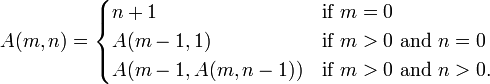
\includegraphics[scale=.6]{graphics/0ae4053de098cc9554752b190a38bc56.png}
% \caption{ A(m, n) = \textbackslash{}begin\{cases\} n+1 \&
% \textbackslash{}mbox\{if \} m = 0 \textbackslash{}\textbackslash{}
% A(m-1, 1) \& \textbackslash{}mbox\{if \} m \textgreater{} 0
% \textbackslash{}mbox\{ and \} n = 0 \textbackslash{}\textbackslash{}
% A(m-1, A(m, n-1)) \& \textbackslash{}mbox\{if \} m \textgreater{} 0
% \textbackslash{}mbox\{ and \} n \textgreater{} 0.
% \textbackslash{}end\{cases\} }
\end{figure}

Its arguments are never negative and it always terminates. Write a
function which returns the value of \emph{A}(\emph{m},\emph{n}).
Arbitrary precision is preferred (since the function grows so quickly),
but not required.

\begin{wideverbatim}

(de ack (X Y)
   (cond
      ((=0 X) (inc Y))
      ((=0 Y) (ack (dec X) 1))
      (T (ack (dec X) (ack X (dec Y)))) ) )

\end{wideverbatim}

\pagebreak{}
\section*{Active Directory/Connect}

The task is to establish a connection to an Active Directory or
Lightweight Directory Access Protocol server.

\begin{wideverbatim}

(unless (=0 (setq Ldap (native "libldap.so" "ldap_open" 'N "example.com" 389)))
   (quit "Can't open LDAP") )

(native "libldap.so" "ldap_simple_bind_s" 'I Ldap "user" "password")

\end{wideverbatim}

\pagebreak{}
\section*{Active Directory/Search for a user}

Make sure you Connect to Active Directory

\begin{wideverbatim}

(de ldapsearch (Sn)
   (in
      (list "ldapsearch" "-xH" "ldap://db.debian.org"
         "-b" "dc=debian,dc=org"
         (pack "sn=" Sn) )
      (list
         (cons 'cn (prog (from "cn: ") (line T)))
         (cons 'uid (prog (from "uid: ") (line T))) ) ) )

Test:

: (ldapsearch "Fischer")
-> ((cn . "Mika") (uid . "mf"))

\end{wideverbatim}

\pagebreak{}
\section*{Active object}

In object-oriented programming an object is active when its state
depends on clock. Usually an active object encapsulates a task that
updates the object's state. To the outer world the object looks like a
normal object with methods that can be called from outside.
Implementation of such methods must have a certain synchronization
mechanism with the encapsulated task in order to prevent object's
state corruption.

A typical instance of an active object is an animation widget. The
widget state changes with the time, while as an object it has all
properties of a normal widget.

% Animation is the foundation of a great many parts of graphical user
% interfaces, including both the fancy effects when things change used in
% window managers, and of course games. The core of any animation system
% is a scheme for periodically changing the display while still remaining
% responsive to the user. This task demonstrates this.

% Create a window containing the string "\texttt{Hello World! }" (the
% trailing space is significant). Make the text appear to be rotating
% right by periodically removing one letter from the end of the string and
% attaching it to the front. When the user clicks on the text, it should
% reverse its direction.

\textbf{The task}

Implement an active integrator object. The object has an input and
output. The input can be set using the method \emph{Input}. The input is
a function of time. The output can be queried using the method
\emph{Output}. The object integrates its input over the time and the
result becomes the object's output. So if the input is
\emph{K}(\emph{t}) and the output is \emph{S}, the object state \emph{S}
is changed to \emph{S} + (\emph{K}(\emph{t}\textsubscript{1}) +
\emph{K}(\emph{t}\textsubscript{0})) * (\emph{t}\textsubscript{1} -
\emph{t}\textsubscript{0}) / 2, i.e. it integrates \emph{K} using the
trapeze method. Initially \emph{K} is constant 0 and \emph{S} is 0.

In order to test the object:

\begin{enumerate}
\item
  set its input to sin (2$\pi$ \emph{f t}), where the frequency
  \emph{f}=0.5Hz. The phase is irrelevant.
\item
  wait 2s
\item
  set the input to constant 0
\item
  wait 0.5s
\end{enumerate}

Verify that now the object's output is approximately 0 (the sine has
the period of 2s). The accuracy of the result will depend on the OS
scheduler time slicing and the accuracy of the clock.



\begin{wideverbatim}

(load "@lib/math.l")

(class +Active)
# inp val sum usec

(dm T ()
   (unless (assoc -100 *Run)           # Install timer task
      (task -100 100                   # Update objects every 0.1 sec
         (mapc 'update> *Actives) ) )
   (=: inp '((U) 0))                   # Set zero input function
   (=: val 0)                          # Initialize last value
   (=: sum 0)                          # Initialize sum
   (=: usec (usec))                    # and time
   (push '*Actives This) )             # Install in notification list

(dm input> (Fun)
   (=: inp Fun) )

(dm update> ()
   (let (U (usec)  V ((: inp) U))      # Get current time, calculate value
      (inc (:: sum)
         (*/
            (+ V (: val))              # (K(t[1]) + K(t[0])) *
            (- U (: usec))             # (t[1] - t[0]) /
            2.0 ) )                    # 2.0
      (=: val V)
      (=: usec U) ) )

(dm output> ()
   (format (: sum) *Scl) )             # Get result

(dm stop> ()
   (unless (del This '*Actives)        # Removing the last active object?
      (task -100) ) )                  # Yes: Uninstall timer task

(de integrate ()                       # Test it
   (let Obj (new '(+Active))           # Create an active object
      (input> Obj                      # Set input function
         '((U) (sin (*/ pi U 1.0))) )  # to sin(π * t)
      (wait 2000)                      # Wait 2 sec
      (input> Obj '((U) 0))            # Reset input function
      (wait 500)                       # Wait 0.5 sec
      (prinl "Output: " (output> Obj)) # Print return value
      (stop> Obj) ) )                  # Stop active object

\end{wideverbatim}

\pagebreak{}
\section*{Add a variable to a class instance at runtime}

Demonstrate how to dynamically add variables to an object (a class
instance) at runtime.

This is useful when the methods/variables of an instance are based on
a data file that isn't available until runtime. Hal Fulton gives an
example of creating an OO CSV parser at
\href{http://www.devsource.com/article2/0,1759,1928562,00.asp}{An
  Exercise in Metaprogramming with Ruby}. This is referred to as
``monkeypatching'' by Pythonistas and some others.


\begin{wideverbatim}

In general, all instance variables in PicoLisp are dynamically created at
runtime.

: (setq MyObject (new '(+MyClass)))       # Create some object
-> \$385605941
: (put MyObject 'newvar '(some value))    # Set variable
-> (some value)
: (show MyObject)                         # Show the object
\$385605941 (+MyClass)
   newvar (some value)
-> \$385605941

\end{wideverbatim}

\pagebreak{}
\section*{Address of a variable}

\textbf{Basic Data Operation:} This is a basic data operation. It
represents a fundamental action on a basic data type.

You may see other such operations in the Basic Data Operations
category, or:

\textbf{Integer Operations:} Arithmetic \textbar{} Comparison

\textbf{Boolean Operations:} Bitwise \textbar{} Logical

\textbf{String Operations:} Concatenation \textbar{} Interpolation
\textbar{} Matching

\textbf{Memory Operations:} Pointers \& references \textbar{} \textbf{Addresses}

Demonstrate how to get the address of a variable and how to set the
address of a variable.


\begin{wideverbatim}

The PicoLisp function '[http://software-lab.de/doc/refA.html#adr adr]' returns
the address of a variable. A variable may be either a symbol or a cons pair in
PicoLisp.

The returned address is a number representing an encoded pointer. For symbols,
it is a negative number, and for cons pairs a positive number. The same function
'adr' can then be used to convert that pointer back to the original object.

: (setq X 7)
-> 7

: (adr 'X)
-> -2985527269106

: (val (adr -2985527269106))
-> 7

: (set (adr -2985527269106) '(a b c))
-> (a b c)

: X
-> (a b c)

\end{wideverbatim}

\pagebreak{}
\section*{Align columns}

Given a text file of many lines, where fields within a line are
delineated by a single `dollar' character, write a program that aligns
each column of fields by ensuring that words in each column are
separated by at least one space. Further, allow for each word in a
column to be either left justified, right justified, or center
justified within its column.

Use the following text to test your programs:

\begin{wideverbatim}
Given$a$text$file$of$many$lines,$where$fields$within$a$line$
are$delineated$by$a$single$'dollar'$character,$write$a$program
that$aligns$each$column$of$fields$by$ensuring$that$words$in$each$
column$are$separated$by$at$least$one$space.
Further,$allow$for$each$word$in$a$column$to$be$either$left$
justified,$right$justified,$or$center$justified$within$its$column.
\end{wideverbatim}

Note that:

\begin{enumerate}
\item
  The example input texts lines may, or may not, have trailing dollar
  characters.
\item
  All columns should share the same alignment.
\item
  Consecutive space characters produced adjacent to the end of lines are
  insignificant for the purposes of the task.
\item
  Output text will be viewed in a mono-spaced font on a plain text
  editor or basic terminal.
\item
  The minimum space between columns should be computed from the text and
  not hard-coded.
\item
  It is \emph{not} a requirement to add separating characters between or
  around columns.
\end{enumerate}



\begin{wideverbatim}

(let Sizes NIL                         # Build a list of sizes
   (let Lines                          # and of lines
      (make
         (in "input.txt"                     # Reading input file
            (while (split (line) "$")        # delimited by '$'
               (let (L (link (mapcar pack @))  S Sizes)
                  (setq Sizes                   # Maintain sizes
                     (make
                        (while (or L S)
                           (link
                              (max
                                 (inc (length (pop 'L)))
                                 (pop 'S) ) ) ) ) ) ) ) ) )
      (for L Lines                                 # Print lines
         (prinl (apply align L (mapcar - Sizes))) )   # left aligned
      (prinl)
      (for L Lines
         (prinl (apply align L Sizes)) )              # right aligned
      (prinl)
      (for L Lines
         (prinl (apply center L Sizes)) ) ) )         # and centered

\end{wideverbatim}

\pagebreak{}
\section*{Amb}

Define and give an example of the \emph{\textbf{Amb}} operator.

The Amb operator takes some number of expressions (or values if that's
simpler in the language) and nondeterministically yields the one or
fails if given no parameter, amb returns the value that doesn't lead to
failure.

The example is using amb to choose four words from the following
strings:

set 1: ``the'' ``that'' ``a''

set 2: ``frog'' ``elephant'' ``thing''

set 3: ``walked'' ``treaded'' ``grows''

set 4: ``slowly'' ``quickly''

It is a failure if the last character of word 1 is not equal to the
first character of word 2, and similarly with word 2 and word 3, as well
as word 3 and word 4. (the only successful sentence is ``that thing
grows slowly'').


\begin{wideverbatim}

For backtracking, Pilog (PicoLisp Prolog) is the natural choice.

(be amb (@E @Lst)
   (lst @E @Lst) )

(be joins (@Left @Right)
   (@T last (chop (-> @Left)))
   (@R car (chop (-> @Right)))
   (or
      ((equal @T @R))
      ((amb @ NIL)) ) )  # Explicitly using amb fail as required

(be ambExample ((@Word1 @Word2 @Word3 @Word4))
  (amb @Word1 ("the" "that" "a"))
  (amb @Word2 ("frog" "elephant" "thing"))
  (amb @Word3 ("walked" "treaded" "grows"))
  (amb @Word4 ("slowly" "quickly"))
  (joins @Word1 @Word2)
  (joins @Word2 @Word3)
  (joins @Word3 @Word4) )

Output:

: (? (ambExample @Result))
 @Result=("that" "thing" "grows" "slowly")
-> NIL

\end{wideverbatim}

\pagebreak{}
\section*{Anagrams}

Two or more words can be composed of the same characters, but in a
different order. Using the word list at
\href{http://www.puzzlers.org/pub/wordlists/unixdict.txt}{http://www.puzzlers.org/pub/wordlists/unixdict.txt},
find the sets of words that share the same characters that contain the
most words in them.


\begin{wideverbatim}

A straight-forward implementation using 'group' takes 48 seconds
on a 1.7 GHz Pentium:

(flip
   (by length sort
      (by '((L) (sort (copy L))) group
         (in "unixdict.txt" (make (while (line) (link @)))) ) ) )

Using a binary tree with the 'idx' function, it takes only 0.42 seconds
on the same machine, a factor of 100 faster:

(let Words NIL
   (in "unixdict.txt"
      (while (line)
         (let (Word (pack @)  Key (pack (sort @)))
            (if (idx 'Words Key T)
               (push (car @) Word)
               (set Key (list Word)) ) ) ) )
   (flip (by length sort (mapcar val (idx 'Words)))) )

Output:

-> (("vile" "veil" "live" "levi" "evil") ("trace" "crate" "cater" "carte" "caret
") ("regal" "large" "lager" "glare" "alger") ("neal" "lena" "lean" "lane" "elan"
) ("lange" "glean" "galen" "angle" "angel") ("elba" "bela" "bale" "able" "abel")
 ("tulsa" "talus" "sault" "latus") ...

\end{wideverbatim}

\pagebreak{}
\section*{Anagrams/Deranged anagrams}

Two or more words are said to be anagrams if they have the same
characters, but in a different order. By analogy with derangements we
define a deranged anagram as two words with the same characters, but
in which the same character does \emph{not} appear in the same
position in both words.

The task is to use the word list at
\href{http://www.puzzlers.org/pub/wordlists/unixdict.txt}{http://www.puzzlers.org/pub/wordlists/unixdict.txt}
to find and \emph{show} the longest deranged anagram.

Cf.

\begin{itemize}
\item
  Permutations/Derangements
\item
  Best shuffle
\end{itemize}


\begin{wideverbatim}

(let Words NIL
   (in "unixdict.txt"
      (while (line)
         (let (Word @  Key (pack (sort (copy @))))
            (if (idx 'Words Key T)
               (push (car @) Word)
               (set Key (list Word)) ) ) ) )
   (maxi '((X) (length (car X)))
      (extract
         '((Key)
            (pick
               '((Lst)
                  (and
                     (find
                        '((L) (not (find = L Lst)))
                        (val Key) )
                     (cons (pack @) (pack Lst)) ) )
               (val Key) ) )
         (idx 'Words) ) ) )

Output:

-> ("excitation" . "intoxicate")

\end{wideverbatim}

\pagebreak{}
\section*{Animate a pendulum}


One good way of making an animation is by simulating a physical system
and illustrating the variables in that system using a dynamically
changing graphical display. The classic such physical system is a
\href{http://en.wikipedia.org/wiki/Pendulum}{simple gravity pendulum}.

For this task, create a simple physical model of a pendulum and animate
it.



\begin{wideverbatim}

A minimalist solution. The pendulum consists of the center point '+', and the
swinging xterm cursor.

(load "@lib/math.l")

(de pendulum (X Y Len)
   (let (Angle pi/2  V 0)
      (call 'clear)
      (call 'tput "cup" Y X)
      (prin '+)
      (call 'tput "cup" 1 (+ X Len))
      (until (key 25)                        # 25 ms
         (let A (*/ (sin Angle) -9.81 1.0)
            (inc 'V (*/ A 40))               # DT = 25 ms = 1/40 sec
            (inc 'Angle (*/ V 40)) )
         (call 'tput "cup"
            (+ Y (*/ Len (cos Angle) 2.2))   # Compensate for aspect ratio
            (+ X (*/ Len (sin Angle) 1.0)) ) ) ) )

Test (hit any key to stop):

(pendulum 40 1 36)

\end{wideverbatim}

\pagebreak{}
\section*{Animation}

\textbf{Animation} is the foundation of a great many parts of
graphical user interfaces, including both the fancy effects when
things change used in window managers, and of course games. The core
of any animation system is a scheme for periodically changing the
display while still remaining responsive to the user. This task
demonstrates this.

Create a window containing the string "\texttt{Hello World! }" (the
trailing space is significant). Make the text appear to be rotating
right by periodically removing one letter from the end of the string and
attaching it to the front. When the user clicks on the text, it should
reverse its direction.


\begin{wideverbatim}

Plain text

A plain text version. The following script works in an XTerm window.

#!/usr/bin/picolisp /usr/lib/picolisp/lib.l

(prin "^[[?9h")  # Mouse reporting on

(setq Dir 1  Text (chop "Hello World! "))

(loop
   (prin (do Dir (rot Text)))
   (when (= "^[" (key 200))
      (key) (key)
      (when (= " " (key))  # Left button
         (setq Dir (if (= 1 Dir) 12 1)) )
      (key) (key) )
   (do (length Text) (prin "^H")) )

\end{wideverbatim}

\begin{wideverbatim}

HTML/JavaScript

The standard PicoLisp GUI is HTTP based. Connect your browser to
http://localhost:8080 after starting the following script.

The scrolling text is displayed in a button. Clicking on the button
reverses the scroll direction.

#!/usr/bin/picolisp /usr/lib/picolisp/lib.l

(load "@ext.l" "@lib/http.l" "@lib/xhtml.l" "@lib/form.l")

(one *Dir)

(de start ()
   (app)
   (action
      (html 0 "Animation" "@lib.css" NIL
         (form NIL
            (gui '(+Button)
               '(pack (do *Dir (rot '`(chop "Hello World! "))))
               '(setq *Dir (if (= 1 *Dir) 12 1)) )
            (gui '(+Click +Auto +Button) 400 'This 1000 "Start") ) ) ) )

(server 8080 "!start")
(wait)

\end{wideverbatim}

\begin{wideverbatim}

Java/Swing

This solution works on ErsatzLisp, the Java version of PicoLisp.

#!ersatz/pil

(setq
   Dir 1
   Text (chop "Hello World! ")
   Frame (java "javax.swing.JFrame" T "Animation")
   Label (java "javax.swing.JLabel" T (pack Text)) )

(java Label 'addMouseListener
   (interface "java.awt.event.MouseListener"
      'mouseClicked '((Ev) (setq Dir (if (= 1 Dir) 12 1)))
      'mouseEntered nil
      'mouseExited nil
      'mousePressed nil
      'mouseReleased nil ) )

(java Frame 'add Label)
(java Frame 'pack)
(java Frame 'setVisible T)
(loop
   (wait 200)
   (java Label 'setText (pack (do Dir (rot Text)))) )

\end{wideverbatim}

\pagebreak{}
\section*{Anonymous recursion}


While implementing a recursive function, it often happens that we must
resort to a separate ``helper function'' to handle the actual recursion.

This is usually the case when directly calling the current function
would waste too many resources (stack space, execution time), cause
unwanted side-effects, and/or the function doesn't have the right
arguments and/and return values.

So we end up inventing some silly name like ``foo2'' or ``foo\_helper''.
I have always found it painful to come up with a proper name, and see a
quite some disadvantages:

\begin{itemize}
\item
  You have to think up a name, which then pollutes the namespace
\item
  A function is created which is called from nowhere else
\item
  The program flow in the source code is interrupted
\end{itemize}

Some languages allow you to embed recursion directly in-place. This
might work via a label, a local \emph{gosub} instruction, or some
special keyword.

Anonymous recursion can also be accomplished using the
\emph{Y combinator}.

If possible, demonstrate this by writing the recursive version of the
fibonacci function (see \emph{Fibonacci sequence}) which checks for a
negative argument before doing the actual recursion.



\begin{wideverbatim}

(de fibo (N)
   (if (lt0 N)
      (quit "Illegal argument" N) )
   (recur (N)
      (if (> 2 N)
         1
         (+ (recurse (dec N)) (recurse (- N 2))) ) ) )

Explanation: The above uses the
'[http://software-lab.de/doc/refR.html#recur recur]' /
'[http://software-lab.de/doc/refR.html#recurse recurse]' function pair, which is
defined as a standard language extensions as

(de recur recurse
   (run (cdr recurse)) )

Note how 'recur' dynamically defines the function 'recurse' at runtime, by
binding the rest of the expression (i.e. the body of the 'recur' statement) to
the symbol 'recurse'.

\end{wideverbatim}

\pagebreak{}
\section*{Apply a callback to an array}


In this task, the goal is to take a combined set of elements and apply a
function to each element.



\begin{wideverbatim}

: (mapc println (1 2 3 4 5))  # Print numbers
1
2
3
4
5
-> 5

: (mapcar '((N) (* N N)) (1 2 3 4 5))  # Calculate squares
-> (1 4 9 16 25)

: (mapcar ** (1 2 3 4 5) (2 .))  # Same, using a circular list
-> (1 4 9 16 25)

: (mapcar if '(T NIL T NIL) '(1 2 3 4) '(5 6 7 8))  # Conditional function
-> (1 6 3 8)

\end{wideverbatim}

\pagebreak{}
\section*{Arbitrary-precision integers (included)}


Using the in-built capabilities of your language, calculate the integer
value of:

\begin{figure}[H]
\centering
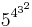
\includegraphics[scale=.9]{graphics/2869715b8204450d9946d9dd1966f50f.png}
% \caption{5\^{}\{4\^{}\{3\^{}2\}\}}
\end{figure}

\begin{itemize}
\item
  Confirm that the first and last twenty digits of the answer are: \\
  \texttt{62060698786608744707...92256259918212890625}
\item
  Find and show the number of decimal digits in the answer.
\end{itemize}

C.F. \href{/wiki/Long\_multiplication}{Long multiplication}

Note:

\begin{itemize}
\item Do not submit an \emph{implementation} of
  \href{http://en.wikipedia.org/wiki/arbitrary\_precision\_arithmetic}{arbitrary
    precision arithmetic}. The intention is to show the capabilities
  of the language as supplied. If a language has a \emph{single,
    overwhelming, library} of varied modules that is endorsed by its
  home site -- such as \emph{CPAN} for Perl or \emph{Boost} for C++ --
  then that \emph{may} be used instead.
\item
  Strictly speaking, this should not be solved by fixed-precision
  numeric libraries where the precision has to be manually set to a
  large value; although if this is the \textbf{only} recourse then it
  may be used with a note explaining that the precision must be set
  manually to a large enough value.
\end{itemize}

\begin{wideverbatim}

(let L (chop (** 5 (** 4 (** 3 2))))
   (prinl (head 20 L) "..." (tail 20 L))
   (length L) )

Output:

62060698786608744707...92256259918212890625
-> 183231

\end{wideverbatim}

\pagebreak{}
\section*{Arena storage pool}

Dynamically allocated objects take their memory from a \emph{heap}.
The memory for an object is provided by an \textbf{allocator} which
maintains the storage pool used for the \emph{heap}. Often a call to
allocator is denoted as

\begin{wideverbatim}
   P := new T
\end{wideverbatim}

where T is the type of an allocated object and P is a \emph{reference}
to the object.

The storage pool chosen by the allocator can be determined by either:

\begin{itemize}
\item
  the object type T;
\item
  the type of pointer P.
\end{itemize}

In the former case objects can be allocated only in one storage pool.
In the latter case objects of the type can be allocated in any storage
pool or on the \emph{stack}.

\textbf{Task description}\\ The task is to show how allocators and
user-defined storage pools are supported by the language. In particular:

\begin{enumerate}
\item
  define an arena storage pool. An arena is a pool in which objects are
  allocated individually, but freed by groups.
\item
  allocate some objects (e.g., integers) in the pool.
\end{enumerate}

Explain what controls the storage pool choice in the language.



\begin{wideverbatim}

PicoLisp allocates any kind of data from a single pool, because everything
is built out of a "cell" primitive. Most of this allocation happens
automatically, but can also be done explicitly with
'[http://software-lab.de/doc/refN.html#new new]' or
'[http://software-lab.de/doc/refB.html#box box]'. For memory-allocated
objects, there is no explicit way of freeing them. Database objects can be
freed with '[http://software-lab.de/doc/refZ.html#zap zap]'.

\end{wideverbatim}

\pagebreak{}
\section*{Arithmetic evaluation}


Create a program which parses and evaluates arithmetic expressions.

\begin{description}
\item[Requirements]
\end{description}

\begin{itemize}
\item
  An
  \href{http://en.wikipedia.org/wiki/Abstract\_syntax\_tree}{abstract-syntax
  tree} (AST) for the expression must be created from parsing the input.
\item
  The AST must be used in evaluation, also, so the input may not be
  directly evaluated (e.g. by calling eval or a similar language
  feature.)
\item
  The expression will be a string or list of symbols like ``(1+3)*7''.
\item
  The four symbols + - * / must be supported as binary operators with
  conventional precedence rules.
\item
   Precedence-control parentheses must also be supported.
\end{itemize}

\begin{description}
\item[Note]
\end{description}

For those who don't remember, mathematical precedence is as follows:

\begin{itemize}
\item
  Parentheses
\item
  Multiplication/Division (left to right)
\item
  Addition/Subtraction (left to right)
\end{itemize}

\begin{description}
\item[C.f]
\end{description}

\begin{itemize}
\item
  \emph{24 game Player}.
\item
  \emph{Parsing/RPN calculator algorithm}.
\item
  \emph{Parsing/RPN to infix conversion}.
\end{itemize}


\begin{wideverbatim}

The built-in function 'str' splits a string into a list of lexical tokens
(numbers and transient symbols). From that, a recursive descendent parser can
build an expression tree, resulting in directly executable Lisp code.

(de ast (Str)
   (let *L (str Str "")
      (aggregate) ) )

(de aggregate ()
   (let X (product)
      (while (member (car *L) '("+" "-"))
         (setq X (list (intern (pop '*L)) X (product))) )
      X ) )

(de product ()
   (let X (term)
      (while (member (car *L) '("*" "/"))
         (setq X (list (intern (pop '*L)) X (term))) )
      X ) )

(de term ()
   (let X (pop '*L)
      (cond
         ((num? X) X)
         ((= "+" X) (term))
         ((= "-" X) (list '- (term)))
         ((= "(" X) (prog1 (aggregate) (pop '*L)))) ) ) )

Output:

: (ast "1+2+3*-4/(1+2)")
-> (+ (+ 1 2) (/ (* 3 (- 4)) (+ 1 2)))

: (ast "(1+2+3)*-4/(1+2)")
-> (/ (* (+ (+ 1 2) 3) (- 4)) (+ 1 2))

\end{wideverbatim}

\pagebreak{}
\section*{Arithmetic-geometric mean}

Write a function to compute the
\href{http://en.wikipedia.org/wiki/Arithmetic-geometric\_mean}{arithmetic-geometric
  mean} of two numbers. The arithmetic-geometric mean of two numbers
can be (usefully) denoted as agm(\emph{a},\emph{g}), and is equal to
the limit of the sequence:

\begin{figure}[H]
\centering

\includegraphics[scale=.6]{graphics/da869c8260ae3107ca34619fd2642642.png}
% \caption{a\_0 = a; \textbackslash{}qquad g\_0 = g}
\end{figure}

\begin{figure}[H]
\centering
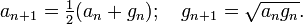
\includegraphics[scale=.6]{graphics/7416c556a1ecfe80d64f32dbc9c18ae6.png}
% \caption{a\_\{n+1\} = \textbackslash{}tfrac\{1\}\{2\}(a\_n + g\_n);
% \textbackslash{}quad g\_\{n+1\} = \textbackslash{}sqrt\{a\_n g\_n\}.}
\end{figure}

Since the limit of \emph{a}\textsubscript{\emph{n}} −
\emph{g}\textsubscript{\emph{n}} tends (rapidly) to zero with
iterations, this is an efficient method.

Demonstrate the function by calculating:

\begin{figure}[H]
\centering
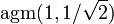
\includegraphics[scale=.6]{graphics/953f4c8f564b5ed18e1b31d2716b5f8c.png}
% \caption{\textbackslash{}mathrm\{agm\}(1,1/\textbackslash{}sqrt\{2\})}
\end{figure}



\begin{wideverbatim}

(scl 80)

(de agm (A G)
   (do 7
      (prog1 (/ (+ A G) 2)
         (setq G (sqrt (* A G))  A @) ) ) )

(round
   (agm 1.0 (*/ 1.0 1.0 (sqrt (* 2.0 1.0))))
   70 )

Output:
-> "0.8472130847939790866064991234821916364814459103269421850605793726597340"

\end{wideverbatim}

\pagebreak{}
\section*{Arithmetic/Complex}

A \textbf{\href{http://en.wikipedia.org/wiki/Complex\_number}{complex
number}} is a number which can be written as
"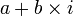
\includegraphics[scale=.6]{graphics/af18dab590e0f994693fc34b6803c1e1.png}"
(sometimes shown as
"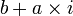
\includegraphics[scale=.6]{graphics/1465b5194836899e7331a9fcf9cda03e.png}")
where a and b are real numbers and
\href{http://en.wikipedia.org/wiki/Imaginary\_unit}{\emph{i} is the
square root of -1}. Typically, complex numbers are represented as a pair
of real numbers called the ``imaginary part'' and ``real part'', where
the imaginary part is the number to be multiplied by \emph{i}.

\begin{itemize}
\item
  Show addition, multiplication, negation, and inversion of complex
  numbers in separate functions. (Subtraction and division operations
  can be made with pairs of these operations.) Print the results for
  each operation tested.
\item
  \emph{Optional:} Show complex conjugation. By definition, the
  \href{http://en.wikipedia.org/wiki/complex\_conjugate}{complex
  conjugate} of \emph{a} + \emph{b}\emph{i} is \emph{a} −
  \emph{b}\emph{i}.
\end{itemize}

Some languages have complex number libraries available. If your language
does, show the operations. If your language does not, also show the
definition of this type.


\begin{wideverbatim}

(load "@lib/math.l")

(de addComplex (A B)
   (cons
      (+ (car A) (car B))        # Real
      (+ (cdr A) (cdr B)) ) )    # Imag

(de mulComplex (A B)
   (cons
      (-
         (*/ (car A) (car B) 1.0)
         (*/ (cdr A) (cdr B) 1.0) )
      (+
         (*/ (car A) (cdr B) 1.0)
         (*/ (cdr A) (car B) 1.0) ) ) )

(de invComplex (A)
   (let Denom
      (+
         (*/ (car A) (car A) 1.0)
         (*/ (cdr A) (cdr A) 1.0) )
      (cons
         (*/ (car A) 1.0 Denom)
         (- (*/ (cdr A) 1.0 Denom)) ) ) )

(de negComplex (A)
   (cons (- (car A)) (- (cdr A))) )

(de fmtComplex (A)
   (pack
      (round (car A) (dec *Scl))
      (and (gt0 (cdr A)) "+")
      (round (cdr A) (dec *Scl))
      "i" ) )

(let (A (1.0 . 1.0)  B (cons pi 1.2))
   (prinl "A = " (fmtComplex A))
   (prinl "B = " (fmtComplex B))
   (prinl "A+B = " (fmtComplex (addComplex A B)))
   (prinl "A*B = " (fmtComplex (mulComplex A B)))
   (prinl "1/A = " (fmtComplex (invComplex A)))
   (prinl "-A = " (fmtComplex (negComplex A))) )

Output:

A = 1.00000+1.00000i
B = 3.14159+1.20000i
A+B = 4.14159+2.20000i
A*B = 1.94159+4.34159i
1/A = 0.50000-0.50000i
-A = -1.00000-1.00000i

\end{wideverbatim}

\pagebreak{}
\section*{Arithmetic/Rational}

The objective of this task is to create a reasonably complete
implementation of rational arithmetic in the particular language using
the idioms of the language.

For example: Define a new type called \textbf{frac} with binary operator
``//'' of two integers that returns a \textbf{structure} made up of the
numerator and the denominator (as per a rational number).

Further define the appropriate rational unary \textbf{operators}
\textbf{abs} and '-', with the binary \textbf{operators} for addition
`+', subtraction '-', multiplication `×', division `/', integer division
`÷', modulo division, the comparison operators (e.g. `\textless{}', `≤',
`\textgreater{}', \& `≥') and equality operators (e.g. `=' \& `≠').

Define standard coercion \textbf{operators} for casting \textbf{int} to
\textbf{frac} etc.

If space allows, define standard increment and decrement
\textbf{operators} (e.g. `+:=' \& '-:=' etc.).

Finally test the operators: Use the new type \textbf{frac} to find all
\emph{perfect numbers} less than 2\textsuperscript{19} by summing the
reciprocal of the factors.

\textbf{See also}

\begin{itemize}
\item
  \emph{Perfect Numbers}
\end{itemize}


\begin{wideverbatim}

(load "@lib/frac.l")

(for (N 2  (> (** 2 19) N)  (inc N))
   (let (Sum (frac 1 N)  Lim (sqrt N))
      (for (F 2  (>= Lim F) (inc F))
         (when (=0 (\% N F))
            (setq Sum
               (f+ Sum
                  (f+ (frac 1 F) (frac 1 (/ N F))) ) ) ) )
      (when (= 1 (cdr Sum))
         (prinl
            "Perfect " N
            ", sum is " (car Sum)
            (and (= 1 (car Sum)) ": perfect") ) ) ) )

Output:

Perfect 6, sum is 1: perfect
Perfect 28, sum is 1: perfect
Perfect 120, sum is 2
Perfect 496, sum is 1: perfect
Perfect 672, sum is 2
Perfect 8128, sum is 1: perfect
Perfect 30240, sum is 3
Perfect 32760, sum is 3
Perfect 523776, sum is 2
\end{wideverbatim}

\pagebreak{}
\section*{Arithmetic/Integer}

\textbf{Basic Data Operation}\\ This is a basic data operation. It
represents a fundamental action on a basic data type.

You may see other such operations in the
\emph{Basic Data Operations}
category, or:

\textbf{Integer Operations} \\ \emph{Arithmetic} \textbar{}
\emph{Comparison}

\textbf{Boolean Operations} \\ \emph{Bitwise}
\textbar{} \emph{Logical}

\textbf{String Operations} \\
\emph{Concatenation} \textbar{}
\emph{Interpolation} \textbar{}
\emph{Matching}

\textbf{Memory Operations} \\
\emph{Pointers \& references}
\textbar{} \emph{Addresses}

Get two integers from the user, and then output the sum, difference,
product, integer quotient and remainder of those numbers. Don't include
error handling. For quotient, indicate how it rounds (e.g. towards 0,
towards negative infinity, etc.). For remainder, indicate whether its
sign matches the sign of the first operand or of the second operand, if
they are different.

Also include the exponentiation operator if one exists.

\begin{wideverbatim}

(de math (A B)
   (prinl "Add      " (+ A B))
   (prinl "Subtract " (- A B))
   (prinl "Multiply " (* A B))
   (prinl "Divide   " (/ A B))        # Truncates towards zero
   (prinl "Div/rnd  " (*/ A B))       # Rounds to next integer
   (prinl "Modulus  " (\% A B))        # Sign of the first operand
   (prinl "Power    " (** A B)) )

\end{wideverbatim}

\pagebreak{}
\section*{Array concatenation}

Show how to concatenate two arrays in your language. If this is as
simple as \texttt{array1 + array2}, so be it.

\begin{wideverbatim}

PicoLisp has no built-in array data type. Lists are used instead.

There are destructive concatenations:

: (setq  A (1 2 3)  B '(a b c))
-> (a b c)
: (conc A B)                        # Concatenate lists in 'A' and 'B'
-> (1 2 3 a b c)
: A
-> (1 2 3 a b c)                    # Side effect: List in 'A' is modified!

and non-destructive concatenations:

: (setq  A (1 2 3)  B '(a b c))
-> (a b c)
: (append A B)                      # Append lists in 'A' and 'B'
-> (1 2 3 a b c)
: A
-> (1 2 3)
: B
-> (a b c)                          # Arguments are not modified

\end{wideverbatim}

\pagebreak{}
\section*{Arrays}

This task is about arrays. For hashes or associative arrays, please see
\emph{Creating an Associative Array}.

In this task, the goal is to show basic array syntax in your language.
Basically, create an array, assign a value to it, and retrieve an
element. (if available, show both fixed-length arrays and dynamic
arrays, pushing a value into it.)

\textbf{See also}

\begin{itemize}
\item
  \emph{Collections}
\item
  \emph{Two-dimensional array (runtime)}
\end{itemize}


\begin{wideverbatim}

PicoLisp has no built-in array data type. Lists are used instead.

(setq A '((1 2 3) (a b c) ((d e) NIL 777)))  # Create a 3x3 structure
(mapc println A)  # Show it

Output:

(1 2 3)
(a b c)
((d e) NIL 777)

Replace 'b' with 'B' in middle row:

(set (nth A 2 2) 'B)
(mapc println A)

Output:

(1 2 3)
(a B c)
((d e) NIL 777)

Insert '1' in front of the middle row:

(push (cdr A) 1)
(mapc println A)

Output:

(1 2 3)
(1 a B c)
((d e) NIL 777)

Append '9' to the middle row:

(queue (cdr A) 9)
(mapc println A)

Output:

(1 2 3)
(1 a B c 9)
((d e) NIL 777)

\end{wideverbatim}

\pagebreak{}
\section*{Assertions}

Assertions are a way of breaking out of code when there is an error or
an unexpected input. Some languages throw \emph{exceptions} and some
treat it as a break point.

Show an assertion in your language by asserting that an integer variable
is equal to 42.

\begin{wideverbatim}

The '[http://software-lab.de/doc/refA.html#assert assert]' function, in
combination with the tilde read macro, generates code only in debug mode:

...
~(assert (= N 42))  # Exists only in debug mode
...

Other possibilities are either to break into an error handler:

(let N 41
   (unless (= N 42) (quit "Incorrect N" N)) )  # 'quit' throws an error
41 -- Incorrect N
?

or to stop at a debug break point, allowing to continue with the program:

(let N 41
   (unless (= N 42) (! setq N 42)) )   # '!' is a breakpoint
(setq N 42)                            # Manually fix the value
!                                      # Hit ENTER to leave the breakpoint
-> 42

\end{wideverbatim}

\pagebreak{}
\section*{Associative arrays/Creation}

In this task, the goal is to create an \emph{associative array} (also
known as a dictionary, map, or hash).

\begin{itemize}
\item
  Related task: \emph{Associative arrays/Iteration}
\end{itemize}


\begin{wideverbatim}

Here we use symbol properties. Other possiblities could be index
trees or association lists.

(put 'A 'foo 5)
(put 'A 'bar 10)
(put 'A 'baz 15)
(put 'A 'foo 20)

: (get 'A 'bar)
-> 10

: (get 'A 'foo)
-> 20

: (show 'A)
A NIL
   foo 20
   bar 10
   baz 15

\end{wideverbatim}

\pagebreak{}
\section*{Associative arrays/Iteration}

Show how to iterate over the key-value pairs of an associative array,
and print each pair out. Also show how to iterate just over the keys, or
the values, if there is a separate way to do that in your language.

\begin{itemize}
\item
  Related task: \emph{Associative arrays/Creation}
\end{itemize}


\begin{wideverbatim}

# Using properties

(put 'A 'foo 5)
(put 'A 'bar 10)
(put 'A 'baz 15)

: (getl 'A)                            # Get the whole property list
-> ((15 . baz) (10 . bar) (5 . foo))

: (mapcar cdr (getl 'A))               # Get all keys
-> (baz bar foo)

: (mapcar car (getl 'A))               # Get all values
-> (15 10 5)

# Using an index tree

(idx 'A (def "foo" 5) T)
(idx 'A (def "bar" 10) T)
(idx 'A (def "baz" 15) T)

: A                                    # Get the whole tree
-> ("foo" ("bar" NIL "baz"))

:  (idx 'A)                            # Get all keys
-> ("bar" "baz" "foo")

:  (mapcar val (idx 'A))               # Get all values
-> (10 15 5)

\end{wideverbatim}

\pagebreak{}
\section*{Atomic updates}

Define a data type consisting of a fixed number of `buckets', each
containing a nonnegative integer value, which supports operations to

\begin{enumerate}
\item
  get the current value of any bucket
\item
  remove a specified amount from one specified bucket and add it to
  another, preserving the total of all bucket values, and
  \href{http://en.wikipedia.org/wiki/Clamping\_(graphics)}{clamping} the
  transferred amount to ensure the values remain nonnegative
\end{enumerate}

\begin{center}\rule{3in}{0.4pt}\end{center}

In order to exercise this data type, create one set of buckets, and
start three concurrent tasks:

\begin{enumerate}
\item
  As often as possible, pick two buckets and make their values closer to
  equal.
\item
  As often as possible, pick two buckets and arbitrarily redistribute
  their values.
\item
  At whatever rate is convenient, display (by any means) the total value
  and, optionally, the individual values of each bucket.
\end{enumerate}

The display task need not be explicit; use of e.g. a debugger or trace
tool is acceptable provided it is simple to set up to provide the
display.

\begin{center}\rule{3in}{0.4pt}\end{center}

This task is intended as an exercise in \emph{atomic} operations. The
sum of the bucket values must be preserved even if the two tasks attempt
to perform transfers simultaneously, and a straightforward solution is
to ensure that at any time, only one transfer is actually occurring ---
that the transfer operation is \emph{atomic}.


\begin{wideverbatim}

(de *Buckets . 15)  # Number of buckets

# E/R model
(class +Bucket +Entity)
(rel key (+Key +Number))  # Key  1 .. *Buckets
(rel val (+Number))       # Value 1 .. 999


# Start with an empty DB
(call 'rm "-f" "buckets.db")  # Remove old DB (if any)
(pool "buckets.db")           # Create new DB file


# Create *Buckets buckets with values between 1 and 999
(for K *Buckets
   (new T '(+Bucket)  'key K  'val (rand 1 999)) )
(commit)


# Pick a random bucket
(de pickBucket ()
   (db 'key '+Bucket (rand 1 *Buckets)) )


\end{wideverbatim}

\begin{wideverbatim}

# First process
(unless (fork)
   (seed *Pid)  # Ensure local random sequence
   (loop
      (let (B1 (pickBucket)  B2 (pickBucket))  # Pick two buckets 'B1' and 'B2'
         (dbSync)                              # Atomic DB operation
         (let (V1 (; B1 val)  V2 (; B2 val))   # Get current values
            (cond
               ((> V1 V2)
                  (dec> B1 'val)               # Make them closer to equal
                  (inc> B2 'val) )
               ((> V2 V1)
                  (dec> B2 'val)
                  (inc> B1 'val) ) ) )
         (commit 'upd) ) ) )                   # Close transaction

\end{wideverbatim}

\begin{wideverbatim}

# Second process
(unless (fork)
   (seed *Pid)  # Ensure local random sequence
   (loop
      (let (B1 (pickBucket)  B2 (pickBucket))  # Pick two buckets 'B1' and 'B2'
         (unless (== B1 B2)                    # Found two different ones?
            (dbSync)                              # Atomic DB operation
            (let (V1 (; B1 val)  V2 (; B2 val))   # Get current values
               (cond
                  ((> V1 V2 0)
                     (inc> B1 'val)               # Redistribute them
                     (dec> B2 'val) )
                  ((> V2 V1 0)
                     (inc> B2 'val)
                     (dec> B1 'val) ) ) )
            (commit 'upd) ) ) ) )                 # Close transaction


\end{wideverbatim}

\begin{wideverbatim}

# Third process
(unless (fork)
   (loop
      (dbSync)                         # Atomic DB operation
      (let Lst (collect 'key '+Bucket) # Get all buckets
         (for This Lst                 # Print current values
            (printsp (: val)) )
         (prinl                        # and total sum
            "-- Total: "
            (sum '((This) (: val)) Lst) ) )
      (rollback)
      (wait 2000) ) )                  # Sleep two seconds

(wait)

\end{wideverbatim}

\begin{wideverbatim}

Output:

70 236 582 30 395 215 525 653 502 825 129 769 722 440 708 -- Total: 6801
0 156 566 352 198 263 0 743 0 1316 58 1180 897 0 1072 -- Total: 6801
0 0 424 101 0 0 0 682 0 1809 0 1549 961 0 1275 -- Total: 6801
0 0 0 0 0 0 0 452 0 2226 0 1838 884 0 1401 -- Total: 6801
54 55 56 55 54 55 54 102 54 2363 54 1816 666 55 1308 -- Total: 6801
198 198 197 196 198 198 197 197 196 1903 197 1438 345 197 946 -- Total: 6801
342 344 343 344 344 342 344 343 343 1278 343 992 343 343 413 -- Total: 6801
^C

\end{wideverbatim}

\pagebreak{}
\section*{Averages/Arithmetic mean}

Write a program to find the
\href{http://en.wikipedia.org/wiki/arithmetic\_mean}{mean} (arithmetic
average) of a numeric vector. In case of a zero-length input, since
the mean of an empty set of numbers is ill-defined, the program may
choose to behave in any way it deems appropriate, though if the
programming language has an established convention for conveying math
errors or undefined values, it's preferable to follow it.

See also: \emph{Median}, \emph{Mode}

\begin{wideverbatim}

(de mean (Lst)
   (if (atom Lst)
      0
      (/ (apply + Lst) (length Lst)) ) )

Output:

: (mean (range 1 1000))
-> 500

\end{wideverbatim}


\pagebreak{}
\section*{Averages/Mean angle}

When calculating the
\href{http://en.wikipedia.org/wiki/Mean\_of\_circular\_quantities}{average
  or mean of an angle} one has to take into account how angles wrap
around so that any angle in degrees plus any integer multiple of 360
degrees is a measure of the same angle.

If one wanted an average direction of the wind over two readings where
the first reading was of 350 degrees and the second was of 10 degrees
then just using the Pythagorean average of the numbers yields an answer
of 180 degrees, whereas if you can note that 350 degrees is equivalent
to -10 degrees and so you have two readings at 10 degrees either side of
zero degrees leading to a more fitting mean angle of zero degrees.

To calculate the mean angle of several angles:

\begin{enumerate}
\item
  Assume all angles are on the unit circle and convert them to complex
  numbers expressed in real and imaginary form.
\item
  Compute the Pythagorean mean of the complex numbers.
\item
  Convert the complex mean to polar coordinates whereupon the phase of
  the complex mean is the required angular mean.
\end{enumerate}

(Note that, since the mean is the sum divided by the number of numbers,
and division by a positive real number does not affect the angle, you
can also simply compute the sum for step 2.)

You can alternatively use this formula:

Given the
angles 
\includegraphics[scale=.6]{graphics/e5d832c5ee9a16553e635e05c2892174.png}
the mean is computed by

\begin{figure}[H]
\centering
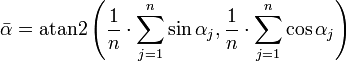
\includegraphics[scale=.6]{graphics/1a4bfb06a8eb34d1ac09405c02d064c4.png}
% \caption{\textbackslash{}bar\{\textbackslash{}alpha\} =
% \textbackslash{}operatorname\{atan2\}\textbackslash{}left(\textbackslash{}frac\{1\}\{n\}\textbackslash{}cdot\textbackslash{}sum\_\{j=1\}\^{}n
% \textbackslash{}sin\textbackslash{}alpha\_j,
% \textbackslash{}frac\{1\}\{n\}\textbackslash{}cdot\textbackslash{}sum\_\{j=1\}\^{}n
% \textbackslash{}cos\textbackslash{}alpha\_j\textbackslash{}right) }
\end{figure}

The task is to:

\begin{enumerate}
\item
  write a function/method/subroutine/\ldots{} that given a list of
  angles in degrees returns their mean angle. (You should use a built-in
  function if you have one that does this for degrees or radians).
\item
  Use the function to compute the means of these lists of angles (in
  degrees): {[}350, 10{]}, {[}90, 180, 270, 360{]}, {[}10, 20, 30{]};
  and show your output here.
\end{enumerate}


\begin{wideverbatim}

(load "@lib/math.l")
 
(de meanAngle (Lst)
   (*/
      (atan2
         (sum '((A) (sin (*/ A pi 180.0))) Lst)
         (sum '((A) (cos (*/ A pi 180.0))) Lst) )
      180.0 pi ) )
 
(for L '((350.0 10.0) (90.0 180.0 270.0 360.0) (10.0 20.0 30.0))
   (prinl
      "The mean angle of ["
      (glue ", " (mapcar round L '(0 .)))
      "] is: " (round (meanAngle L))) )

Output:

The mean angle of [350, 10] is: 0.000
The mean angle of [90, 180, 270, 360] is: 90.000
The mean angle of [10, 20, 30] is: 20.000

\end{wideverbatim}


\pagebreak{}
\section*{Averages/Mean time of day}

A particular activity of bats occurs at these times of the day:

\texttt{23:00:17, 23:40:20, 00:12:45, 00:17:19}

Using the idea that their are twenty four hours in a day which is
analogous to their being 360 degrees in a circle, map times of day to
and from angles and using the ideas of \emph{Averages/Mean angle}
compute and show here the average time of the nocturnal activity to an
accuracy of a second of time.


\begin{wideverbatim}

(load "@lib/math.l")
 
(de meanTime (Lst)
   (let Tim
      (*/
         (atan2
            (sum '((S) (sin (*/ ($tim S) pi 43200))) Lst)
            (sum '((S) (cos (*/ ($tim S) pi 43200))) Lst) )
         43200 pi )
      (tim$ (% (+ Tim 86400) 86400) T) ) )

Test:

: (meanTime '("23:00:17" "23:40:20" "00:12:45" "00:17:19"))
-> "23:47:43"

\end{wideverbatim}

\pagebreak{}
\section*{Averages/Median}

Write a program to find the
\href{http://en.wikipedia.org/wiki/Median}{median} value of a vector
of floating-point numbers. The program need not handle the case where
the vector is empty, but \emph{must} handle the case where there are
an even number of elements.

There are several approaches to this. One is to sort the elements, and
then pick the one in the middle. Sorting would take at least
O(\emph{n}log\emph{n}). Another would be to build a priority queue
from the elements, and then extract half of the elements to get to the
middle one(s). This would also take O(\emph{n}log\emph{n}). The best
solution is to use the
\href{http://en.wikipedia.org/wiki/Selection\_algorithm}{selection
  algorithm} to find the median in O(\emph{n}) time.

See also: \emph{Mean}, \emph{Mode}

\begin{wideverbatim}

(de median (Lst)
   (let N (length Lst)
      (if (bit? 1 N)
         (get (sort Lst) (/ (inc N) 2))
         (setq Lst (nth (sort Lst) (/ N 2)))
         (/ (+ (car Lst) (cadr Lst)) 2) ) ) )

(scl 2)
(prinl (round (median (1.0 2.0 3.0))))
(prinl (round (median (1.0 2.0 3.0 4.0))))
(prinl (round (median (5.1 2.6 6.2 8.8 4.6 4.1))))
(prinl (round (median (5.1 2.6 8.8 4.6 4.1))))

Output:

2.00
2.50
4.85
4.60

\end{wideverbatim}

\pagebreak{}
\section*{Averages/Mode}

Write a program to find the
\href{http://en.wikipedia.org/wiki/Mode\_(statistics)}{mode} value of
a collection. The case where the collection is empty may be ignored.
Care must be taken to handle the case where the mode is non-unique.

If it is not appropriate or possible to support a general collection,
use a vector (array), if possible. If it is not appropriate or possible
to support an unspecified value type, use integers.

See also: \emph{Mean},\emph{Median}

\begin{wideverbatim}

(de modes (Lst)
   (let A NIL
      (for X Lst
         (accu 'A X 1) )
      (mapcar car
         (maxi cdar
            (by cdr group A) ) ) ) )

Output:

: (modes (1 3 6 6 6 6 7 7 12 12 17))
-> (6)

: (modes (1 1 2 4 4))
-> (4 1)

: (modes (chop "ABRAHAMASANTACLARA"))
-> ("A")

: (modes (1 4 A 3 2 7 1 B B 3 6 2 4 C C 5 2 5 B A 3 2 C 3 5 5 4 C 7 7))
-> (5 C 2 3)

\end{wideverbatim}

\pagebreak{}
\section*{Averages/Pythagorean means}


Compute all three of the
\href{http://en.wikipedia.org/wiki/Pythagorean\_means}{Pythagorean
means} of the set of integers 1 through 10.

Show that \\
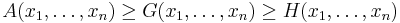
\includegraphics[scale=.6]{graphics/6d547901f0a5fb3819d16aca0048b3ed.png} \\
for this set of positive integers.

\begin{itemize}
\item The most common of the three means, the \emph{arithmetic mean},
  is the sum of the list divided by its length:
\end{itemize}

\begin{figure}[H]
\centering
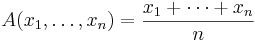
\includegraphics[scale=.6]{graphics/2b72903b5dd461c777da13fde57f3ebb.png}
% \caption{ A(x\_1, \textbackslash{}ldots, x\_n) =
% \textbackslash{}frac\{x\_1 + \textbackslash{}cdots + x\_n\}\{n\}}
\end{figure}

\begin{itemize}
\item
  The \href{http://en.wikipedia.org/wiki/Geometric\_mean}{geometric
  mean} is the \emph{n}th root of the product of the list:
\end{itemize}

\begin{figure}[H]
\centering
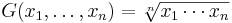
\includegraphics[scale=.6]{graphics/12595bb2b15b5d8b7263aba68c137db3.png}
% \caption{ G(x\_1, \textbackslash{}ldots, x\_n) =
% \textbackslash{}sqrt{[}n{]}\{x\_1 \textbackslash{}cdots x\_n\} }
\end{figure}

\begin{itemize}
\item
  The \href{http://en.wikipedia.org/wiki/Harmonic\_mean}{harmonic mean}
  is \emph{n} divided by the sum of the reciprocal of each item in the
  list:
\end{itemize}

\begin{figure}[H]
\centering
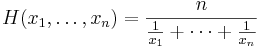
\includegraphics[scale=.6]{graphics/7f1c92a1977747914e9c5127764a9be4.png}
% \caption{ H(x\_1, \textbackslash{}ldots, x\_n) =
% \textbackslash{}frac\{n\}\{\textbackslash{}frac\{1\}\{x\_1\} +
% \textbackslash{}cdots + \textbackslash{}frac\{1\}\{x\_n\}\} }
\end{figure}

C.f. \emph{Averages/Root mean square}


\begin{wideverbatim}

(load "@lib/math.l")

(let (Lst (1.0 2.0 3.0 4.0 5.0 6.0 7.0 8.0 9.0 10.0)  Len (length Lst))
   (prinl "Arithmetic mean: "
      (format
         (/ (apply + Lst) Len)
         *Scl ) )
   (prinl "Geometric mean: "
      (format
         (pow (*/ (apply * Lst) (** 1.0 (dec Len))) (/ 1.0 Len))
         *Scl ) )
   (prinl "Harmonic mean: "
      (format
         (*/ (* 1.0 Len) 1.0 (sum '((N) (*/ 1.0 1.0 N)) Lst))
         *Scl ) ) )

Output:

Arithmetic mean: 5.500000
Geometric mean: 4.528729
Harmonic mean: 3.414172

\end{wideverbatim}

\pagebreak{}
\section*{Averages/Root mean square}

Compute the \href{http://en.wikipedia.org/wiki/Root\_mean\_square}{Root
mean square} of the numbers 1..10.

The root mean square is also known by its initial RMS (or rms), and as
the \textbf{quadratic mean}.

The RMS is calculated as the mean of the squares of the numbers,
square-rooted:

\begin{figure}[H]
\centering
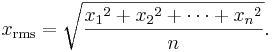
\includegraphics[scale=.6]{graphics/cf22c76e0c33c4fb96262638a28bd52b.png}
% \caption{x\_\{\textbackslash{}mathrm\{rms\}\} = \textbackslash{}sqrt
% \{\{\{x\_1\}\^{}2 + \{x\_2\}\^{}2 + \textbackslash{}cdots +
% \{x\_n\}\^{}2\} \textbackslash{}over n\}. }
\end{figure}

Cf. \emph{Averages/Pythagorean means}


\begin{wideverbatim}

(scl 5)

(let Lst (1.0 2.0 3.0 4.0 5.0 6.0 7.0 8.0 9.0 10.0)
   (prinl
      (format
         (sqrt
            (*/
               (sum '((N) (*/ N N 1.0)) Lst)
               1.0
               (length Lst) )
            T )
         *Scl ) ) )

Output:

6.20484

\end{wideverbatim}

\pagebreak{}
\section*{Averages/Simple moving average}


Computing the
\href{http://en.wikipedia.org/wiki/Moving\_average\#Simple\_moving\_average}{simple
moving average} of a series of numbers.

The task is to:

\emph{Create a \href{http://en.wikipedia.org/wiki/Stateful}{stateful}
function/class/instance that takes a period and returns a routine that
takes a number as argument and returns a simple moving average of its
arguments so far.}

\textbf{Description}\\ A simple moving average is a method for computing
an average of a stream of numbers by only averaging the last P numbers
from the stream, where P is known as the period. It can be implemented
by calling an initialing routine with P as its argument, I(P), which
should then return a routine that when called with individual,
successive members of a stream of numbers, computes the mean of (up to),
the last P of them, lets call this SMA().

The word stateful in the task description refers to the need for SMA()
to remember certain information between calls to it:

\begin{itemize}
\item
  The period, P
\item
  An ordered container of at least the last P numbers from each of its
  individual calls.
\end{itemize}

Stateful also means that successive calls to I(), the initializer,
should return separate routines that do \emph{not} share saved state so
they could be used on two independent streams of data.

Pseudocode for an implementation of SMA is:

\begin{wideverbatim}
function SMA(number: N):
    stateful integer: P
    stateful list:    stream
    number:           average

    stream.append_last(N)
    if stream.length() > P:
        # Only average the last P elements of the stream
        stream.delete_first()
    if stream.length() == 0:
        average = 0
    else:    
        average = sum( stream.values() ) / stream.length()
    return average
\end{wideverbatim}

 See also: \emph{Standard Deviation}


\begin{wideverbatim}

(de sma (@Len)
   (curry (@Len (Data)) (N)
      (push 'Data N)
      (and (nth Data @Len) (con @))  # Truncate
      (*/ (apply + Data) (length Data)) ) )


(def 'sma3 (sma 3))
(def 'sma5 (sma 5))

(scl 2)
(for N (1.0 2.0 3.0 4.0 5.0 5.0 4.0 3.0 2.0 1.0)
   (prinl
      (format N *Scl)
      "   (sma3) "
      (format (sma3 N) *Scl)
      "   (sma5) "
      (format (sma5 N) *Scl) ) )

Output:

1.00   (sma3) 1.00   (sma5) 1.00
2.00   (sma3) 1.50   (sma5) 1.50
3.00   (sma3) 2.00   (sma5) 2.00
4.00   (sma3) 3.00   (sma5) 2.50
5.00   (sma3) 4.00   (sma5) 3.00
5.00   (sma3) 4.67   (sma5) 3.80
4.00   (sma3) 4.67   (sma5) 4.20
3.00   (sma3) 4.00   (sma5) 4.20
2.00   (sma3) 3.00   (sma5) 3.80
1.00   (sma3) 2.00   (sma5) 3.00

\end{wideverbatim}


% %%%%%%%%%%%%%%%%%%%%%%%% referenc.tex %%%%%%%%%%%%%%%%%%%%%%%%%%%%%%
% sample references
% %
% Use this file as a template for your own input.
%
%%%%%%%%%%%%%%%%%%%%%%%% Springer-Verlag %%%%%%%%%%%%%%%%%%%%%%%%%%
%
% BibTeX users please use
% \bibliographystyle{}
% \bibliography{}
%
\biblstarthook{In view of the parallel print and (chapter-wise) online publication of your book at \url{www.springerlink.com} it has been decided that -- as a genreral rule --  references should be sorted chapter-wise and placed at the end of the individual chapters. However, upon agreement with your contact at Springer you may list your references in a single seperate chapter at the end of your book. Deactivate the class option \texttt{sectrefs} and the \texttt{thebibliography} environment will be put out as a chapter of its own.\\\indent
References may be \textit{cited} in the text either by number (preferred) or by author/year.\footnote{Make sure that all references from the list are cited in the text. Those not cited should be moved to a separate \textit{Further Reading} section or chapter.} The reference list should ideally be \textit{sorted} in alphabetical order -- even if reference numbers are used for the their citation in the text. If there are several works by the same author, the following order should be used: 
\begin{enumerate}
\item all works by the author alone, ordered chronologically by year of publication
\item all works by the author with a coauthor, ordered alphabetically by coauthor
\item all works by the author with several coauthors, ordered chronologically by year of publication.
\end{enumerate}
The \textit{styling} of references\footnote{Always use the standard abbreviation of a journal's name according to the ISSN \textit{List of Title Word Abbreviations}, see \url{http://www.issn.org/en/node/344}} depends on the subject of your book:
\begin{itemize}
\item The \textit{two} recommended styles for references in books on \textit{mathematical, physical, statistical and computer sciences} are depicted in ~\cite{science-contrib, science-online, science-mono, science-journal, science-DOI} and ~\cite{phys-online, phys-mono, phys-journal, phys-DOI, phys-contrib}.
\item Examples of the most commonly used reference style in books on \textit{Psychology, Social Sciences} are~\cite{psysoc-mono, psysoc-online,psysoc-journal, psysoc-contrib, psysoc-DOI}.
\item Examples for references in books on \textit{Humanities, Linguistics, Philosophy} are~\cite{humlinphil-journal, humlinphil-contrib, humlinphil-mono, humlinphil-online, humlinphil-DOI}.
\item Examples of the basic Springer style used in publications on a wide range of subjects such as \textit{Computer Science, Economics, Engineering, Geosciences, Life Sciences, Medicine, Biomedicine} are ~\cite{basic-contrib, basic-online, basic-journal, basic-DOI, basic-mono}. 
\end{itemize}
}

\begin{thebibliography}{99.}%
% and use \bibitem to create references.
%
% Use the following syntax and markup for your references if 
% the subject of your book is from the field 
% "Mathematics, Physics, Statistics, Computer Science"
%
% Contribution 
\bibitem{science-contrib} Broy, M.: Software engineering --- from auxiliary to key technologies. In: Broy, M., Dener, E. (eds.) Software Pioneers, pp. 10-13. Springer, Heidelberg (2002)
%
% Online Document
\bibitem{science-online} Dod, J.: Effective substances. In: The Dictionary of Substances and Their Effects. Royal Society of Chemistry (1999) Available via DIALOG. \\
\url{http://www.rsc.org/dose/title of subordinate document. Cited 15 Jan 1999}
%
% Monograph
\bibitem{science-mono} Geddes, K.O., Czapor, S.R., Labahn, G.: Algorithms for Computer Algebra. Kluwer, Boston (1992) 
%
% Journal article
\bibitem{science-journal} Hamburger, C.: Quasimonotonicity, regularity and duality for nonlinear systems of partial differential equations. Ann. Mat. Pura. Appl. \textbf{169}, 321--354 (1995)
%
% Journal article by DOI
\bibitem{science-DOI} Slifka, M.K., Whitton, J.L.: Clinical implications of dysregulated cytokine production. J. Mol. Med. (2000) doi: 10.1007/s001090000086 
%
\bigskip

% Use the following (APS) syntax and markup for your references if 
% the subject of your book is from the field 
% "Mathematics, Physics, Statistics, Computer Science"
%
% Online Document
\bibitem{phys-online} J. Dod, in \textit{The Dictionary of Substances and Their Effects}, Royal Society of Chemistry. (Available via DIALOG, 1999), 
\url{http://www.rsc.org/dose/title of subordinate document. Cited 15 Jan 1999}
%
% Monograph
\bibitem{phys-mono} H. Ibach, H. L\"uth, \textit{Solid-State Physics}, 2nd edn. (Springer, New York, 1996), pp. 45-56 
%
% Journal article
\bibitem{phys-journal} S. Preuss, A. Demchuk Jr., M. Stuke, Appl. Phys. A \textbf{61}
%
% Journal article by DOI
\bibitem{phys-DOI} M.K. Slifka, J.L. Whitton, J. Mol. Med., doi: 10.1007/s001090000086
%
% Contribution 
\bibitem{phys-contrib} S.E. Smith, in \textit{Neuromuscular Junction}, ed. by E. Zaimis. Handbook of Experimental Pharmacology, vol 42 (Springer, Heidelberg, 1976), p. 593
%
\bigskip
%
% Use the following syntax and markup for your references if 
% the subject of your book is from the field 
% "Psychology, Social Sciences"
%
%
% Monograph
\bibitem{psysoc-mono} Calfee, R.~C., \& Valencia, R.~R. (1991). \textit{APA guide to preparing manuscripts for journal publication.} Washington, DC: American Psychological Association.
%
% Online Document
\bibitem{psysoc-online} Dod, J. (1999). Effective substances. In: The dictionary of substances and their effects. Royal Society of Chemistry. Available via DIALOG. \\
\url{http://www.rsc.org/dose/Effective substances.} Cited 15 Jan 1999.
%
% Journal article
\bibitem{psysoc-journal} Harris, M., Karper, E., Stacks, G., Hoffman, D., DeNiro, R., Cruz, P., et al. (2001). Writing labs and the Hollywood connection. \textit{J Film} Writing, 44(3), 213--245.
%
% Contribution 
\bibitem{psysoc-contrib} O'Neil, J.~M., \& Egan, J. (1992). Men's and women's gender role journeys: Metaphor for healing, transition, and transformation. In B.~R. Wainrig (Ed.), \textit{Gender issues across the life cycle} (pp. 107--123). New York: Springer.
%
% Journal article by DOI
\bibitem{psysoc-DOI}Kreger, M., Brindis, C.D., Manuel, D.M., Sassoubre, L. (2007). Lessons learned in systems change initiatives: benchmarks and indicators. \textit{American Journal of Community Psychology}, doi: 10.1007/s10464-007-9108-14.
%
%
% Use the following syntax and markup for your references if 
% the subject of your book is from the field 
% "Humanities, Linguistics, Philosophy"
%
\bigskip
%
% Journal article
\bibitem{humlinphil-journal} Alber John, Daniel C. O'Connell, and Sabine Kowal. 2002. Personal perspective in TV interviews. \textit{Pragmatics} 12:257--271
%
% Contribution 
\bibitem{humlinphil-contrib} Cameron, Deborah. 1997. Theoretical debates in feminist linguistics: Questions of sex and gender. In \textit{Gender and discourse}, ed. Ruth Wodak, 99--119. London: Sage Publications.
%
% Monograph
\bibitem{humlinphil-mono} Cameron, Deborah. 1985. \textit{Feminism and linguistic theory.} New York: St. Martin's Press.
%
% Online Document
\bibitem{humlinphil-online} Dod, Jake. 1999. Effective substances. In: The dictionary of substances and their effects. Royal Society of Chemistry. Available via DIALOG. \\
http://www.rsc.org/dose/title of subordinate document. Cited 15 Jan 1999
%
% Journal article by DOI
\bibitem{humlinphil-DOI} Suleiman, Camelia, Daniel C. O�Connell, and Sabine Kowal. 2002. `If you and I, if we, in this later day, lose that sacred fire...�': Perspective in political interviews. \textit{Journal of Psycholinguistic Research}. doi: 10.1023/A:1015592129296.
%
%
%
\bigskip
%
%
% Use the following syntax and markup for your references if 
% the subject of your book is from the field 
% "Computer Science, Economics, Engineering, Geosciences, Life Sciences"
%
%
% Contribution 
\bibitem{basic-contrib} Brown B, Aaron M (2001) The politics of nature. In: Smith J (ed) The rise of modern genomics, 3rd edn. Wiley, New York 
%
% Online Document
\bibitem{basic-online} Dod J (1999) Effective Substances. In: The dictionary of substances and their effects. Royal Society of Chemistry. Available via DIALOG. \\
\url{http://www.rsc.org/dose/title of subordinate document. Cited 15 Jan 1999}
%
% Journal article by DOI
\bibitem{basic-DOI} Slifka MK, Whitton JL (2000) Clinical implications of dysregulated cytokine production. J Mol Med, doi: 10.1007/s001090000086
%
% Journal article
\bibitem{basic-journal} Smith J, Jones M Jr, Houghton L et al (1999) Future of health insurance. N Engl J Med 965:325--329
%
% Monograph
\bibitem{basic-mono} South J, Blass B (2001) The future of modern genomics. Blackwell, London 
%
\end{thebibliography}


%%%%%%%%%%%%%%%%%%%%% chapter.tex %%%%%%%%%%%%%%%%%%%%%%%%%%%%%%%%%
%
% sample chapter
%
% Use this file as a template for your own input.
%
%%%%%%%%%%%%%%%%%%%%%%%% Springer-Verlag %%%%%%%%%%%%%%%%%%%%%%%%%%
%\motto{Use the template \emph{chapter.tex} to style the various elements of your chapter content.}

\chapter{Rosetta Code Tasks starting with B}

\section*{Balanced brackets}


\textbf{Task}:

\begin{itemize}
\item
  Generate a string with N opening brackets (``\texttt{{[}}'') and N
  closing brackets (``\texttt{{]}}''), in some arbitrary order.
\item
  Determine whether the generated string is \emph{balanced}; that is,
  whether it consists entirely of pairs of opening/closing brackets (in
  that order), none of which mis-nest.
\end{itemize}

\textbf{Examples}:

\begin{verbatim}
   (empty)   OK
   []        OK   ][        NOT OK
   [][]      OK   ][][      NOT OK
   [[][]]    OK   []][[]    NOT OK
\end{verbatim}



\begin{wideverbatim}

(load "@lib/simul.l")  # For 'shuffle'

(de generateBrackets (N)
   (shuffle (make (do N (link "[" "]")))) )

(de checkBrackets (S)
   (let N 0
      (for C S
         (if (= C "[")
            (inc 'N)
            (if2 (= C "]") (=0 N)
               (off N)
               (dec 'N) ) ) )
      (=0 N) ) )

(for N 10
   (prinl (if (checkBrackets (prin (generateBrackets N))) " OK" "not OK")) )

Output:

[] OK
[[]] OK
]]][[[not OK
[[[][]]] OK
[][][[[]]] OK
[]][[[][[]]]not OK
[[[]]][][][][] OK
]][][[[[]][]]][[not OK
[]][][[[][[]]][]][not OK
[[[][]]]]][][[]]][[[not OK

\end{wideverbatim}

\pagebreak{}
\section*{Best shuffle}


Shuffle the characters of a string in such a way that as many of the
character values are in a different position as possible. Print the
result as follows: original string, shuffled string, (score). The score
gives the number of positions whose character value did \emph{not}
change.

For example: \texttt{tree, eetr, (0)}

A shuffle that produces a randomized result among the best choices is to
be preferred. A deterministic approach that produces the same sequence
every time is acceptable as an alternative.

The words to test with are: \texttt{abracadabra}, \texttt{seesaw},
\texttt{elk}, \texttt{grrrrrr}, \texttt{up}, \texttt{a}

Cf.

\begin{itemize}
\item
  \emph{Anagrams/Deranged anagrams}
\item
  \emph{Permutations/Derangements}
\end{itemize}


\begin{wideverbatim}

(de bestShuffle (Str)
   (let Lst NIL
      (for C (setq Str (chop Str))
         (if (assoc C Lst)
            (con @ (cons C (cdr @)))
            (push 'Lst (cons C)) ) )
      (setq Lst (apply conc (flip (by length sort Lst))))
      (let Res
         (mapcar
            '((C)
               (prog1 (or (find <> Lst (circ C)) C)
                  (setq Lst (delete @ Lst)) ) )
            Str )
         (prinl Str " " Res " (" (cnt = Str Res) ")") ) ) )

Output:

: (bestShuffle "abracadabra")
abracadabra raarababadc (0)

: (bestShuffle "seesaw")
seesaw essewa (0)

: (bestShuffle "elk")
elk lke (0)

: (bestShuffle "grrrrrr")
grrrrrr rgrrrrr (5)

: (bestShuffle "up")
up pu (0)

: (bestShuffle "a")
a a (1)

\end{wideverbatim}

\pagebreak{}
\section*{Binary digits}


The task is to output the sequence of binary digits for a given
\href{http://en.wikipedia.org/wiki/Natural\_number}{non-negative
integer}.

The decimal value \texttt{5}, should produce an output of \texttt{101}
The decimal value \texttt{50} should produce an output of
\texttt{110010} The decimal value \texttt{9000} should produce an output
of \texttt{10001100101000}

The results can be achieved using builtin radix functions within the
language, if these are available, or alternatively a user defined
function can be used. The output produced should consist just of the
binary digits of each number followed by a newline. There should be no
other whitespace, radix or sign markers in the produced output, and
\href{http://en.wikipedia.org/wiki/Leading\_zero}{leading zeros} should
not appear in the results.



\begin{wideverbatim}

: (bin 5)
-> "101"

: (bin 50)
-> "110010"

: (bin 9000)
-> "10001100101000"

\end{wideverbatim}

\pagebreak{}
\section*{Binary search}


A binary search divides a range of values into halves, and continues to
narrow down the field of search until the unknown value is found. It is
the classic example of a ``divide and conquer'' algorithm.

As an analogy, consider the children's game "\emph{guess a number}."
The scorer has a secret number, and will only tell the player if their
guessed number is higher than, lower than, or equal to the secret
number. The player then uses this information to guess a new number.

As the player, an optimal strategy for the general case is to start by
choosing the range's midpoint as the guess, and then asking whether the
guess was higher, lower, or equal to the secret number. If the guess was
too high, one would select the point exactly between the range midpoint
and the beginning of the range. If the original guess was too low, one
would ask about the point exactly between the range midpoint and the end
of the range. This process repeats until one has reached the secret
number.

\textbf{The Task}

Given the starting point of a range, the ending point of a range, and
the ``secret value'', implement a binary search through a sorted integer
array for a certain number. Implementations can be recursive or
iterative (both if you can). Print out whether or not the number was in
the array afterwards. If it was, print the index also.

There are several binary search algorithms commonly seen. They differ by
how they treat multiple values equal to the given value, and whether
they indicate whether the element was found or not. For completeness we
will present pseudocode for all of them.

All of the following code examples use an ``inclusive'' upper bound
(i.e. \texttt{high = N-1} initially). Any of the examples can be
converted into an equivalent example using ``exclusive'' upper bound
(i.e. \texttt{high = N} initially) by making the following simple
changes (which simply increase \texttt{high} by 1):

\begin{itemize}
\item
  change \texttt{high = N-1} to \texttt{high = N}
\item
  change \texttt{high = mid-1} to \texttt{high = mid}
\item
  (for recursive algorithm) change \texttt{if (high \textless{} low)} to
  \texttt{if (high \textless{}= low)}
\item
  (for iterative algorithm) change
  \texttt{while (low \textless{}= high)} to
  \texttt{while (low \textless{} high)}
\end{itemize}

Traditional algorithm

The algorithms are as follows (from
\href{http://en.wikipedia.org/wiki/Binary\_search}{Wikipedia}). The
algorithms return the index of some element that equals the given value
(if there are multiple such elements, it returns some arbitrary one). It
is also possible, when the element is not found, to return the
``insertion point'' for it (the index that the value would have if it
were inserted into the array).

\textbf{Recursive Pseudocode}:

\begin{wideverbatim}
  // initially called with low = 0, high = N-1
  BinarySearch(A[0..N-1], value, low, high) {
      // invariants: value > A[i] for all i < low
                     value < A[i] for all i > high
      if (high < low)
          return not_found // value would be inserted at index "low"
      mid = (low + high) / 2
      if (A[mid] > value)
          return BinarySearch(A, value, low, mid-1)
      else if (A[mid] < value)
          return BinarySearch(A, value, mid+1, high)
      else
          return mid
  }
\end{wideverbatim}

\textbf{Iterative Pseudocode}:

\begin{wideverbatim}
  BinarySearch(A[0..N-1], value) {
      low = 0
      high = N - 1
      while (low <= high) {
          // invariants: value > A[i] for all i < low
                         value < A[i] for all i > high
          mid = (low + high) / 2
          if (A[mid] > value)
              high = mid - 1
          else if (A[mid] < value)
              low = mid + 1
          else
              return mid
      }
      return not_found // value would be inserted at index "low"
  }
\end{wideverbatim}

Leftmost insertion point

The following algorithms return the leftmost place where the given
element can be correctly inserted (and still maintain the sorted order).
This is the lower (inclusive) bound of the range of elements that are
equal to the given value (if any). Equivalently, this is the lowest
index where the element is greater than or equal to the given value
(since if it were any lower, it would violate the ordering), or 1 past
the last index if such an element does not exist. This algorithm does
not determine if the element is actually found. This algorithm only
requires one comparison per level.

\textbf{Recursive Pseudocode}:

\begin{wideverbatim}
  // initially called with low = 0, high = N - 1
  BinarySearch_Left(A[0..N-1], value, low, high) {
      // invariants: value > A[i] for all i < low
                     value <= A[i] for all i > high
      if (high < low)
          return low
      mid = (low + high) / 2
      if (A[mid] >= value)
          return BinarySearch_Left(A, value, low, mid-1)
      else
          return BinarySearch_Left(A, value, mid+1, high)
  }
\end{wideverbatim}

\textbf{Iterative Pseudocode}:

\begin{wideverbatim}
  BinarySearch_Left(A[0..N-1], value) {
      low = 0
      high = N - 1
      while (low <= high) {
          // invariants: value > A[i] for all i < low
                         value <= A[i] for all i > high
          mid = (low + high) / 2
          if (A[mid] >= value)
              high = mid - 1
          else
              low = mid + 1
      }
      return low
  }
\end{wideverbatim}

Rightmost insertion point

The following algorithms return the rightmost place where the given
element can be correctly inserted (and still maintain the sorted order).
This is the upper (exclusive) bound of the range of elements that are
equal to the given value (if any). Equivalently, this is the lowest
index where the element is greater than the given value, or 1 past the
last index if such an element does not exist. This algorithm does not
determine if the element is actually found. This algorithm only requires
one comparison per level. Note that these algorithms are almost exactly
the same as the leftmost-insertion-point algorithms, except for how the
inequality treats equal values.

\textbf{Recursive Pseudocode}:

\begin{wideverbatim}
  // initially called with low = 0, high = N - 1
  BinarySearch_Right(A[0..N-1], value, low, high) {
      // invariants: value >= A[i] for all i < low
                     value < A[i] for all i > high
      if (high < low)
          return low
      mid = (low + high) / 2
      if (A[mid] > value)
          return BinarySearch_Right(A, value, low, mid-1)
      else
          return BinarySearch_Right(A, value, mid+1, high)
  }
\end{wideverbatim}

\textbf{Iterative Pseudocode}:

\begin{wideverbatim}
  BinarySearch_Right(A[0..N-1], value) {
      low = 0
      high = N - 1
      while (low <= high) {
          // invariants: value >= A[i] for all i < low
                         value < A[i] for all i > high
          mid = (low + high) / 2
          if (A[mid] > value)
              high = mid - 1
          else
              low = mid + 1
      }
      return low
  }
\end{wideverbatim}

Extra credit

Make sure it does not have overflow bugs.

The line in the pseudocode above to calculate the mean of two integers:

\begin{wideverbatim}
mid = (low + high) / 2
\end{wideverbatim}

could produce the wrong result in some programming languages when used
with a bounded integer type, if the addition causes an overflow. (This
can occur if the array size is greater than half the maximum integer
value.) If signed integers are used, and \texttt{low + high} overflows,
it becomes a negative number, and dividing by 2 will still result in a
negative number. Indexing an array with a negative number could produce
an out-of-bounds exception, or other undefined behavior. If unsigned
integers are used, an overflow will result in losing the largest bit,
which will produce the wrong result.

One way to fix it is to manually add half the range to the low number:

\begin{wideverbatim}
mid = low + (high - low) / 2
\end{wideverbatim}

Even though this is mathematically equivalent to the above, it is not
susceptible to overflow.

Another way for signed integers, possibly faster, is the following:

\begin{wideverbatim}
mid = (low + high) >>> 1
\end{wideverbatim}

where \texttt{ \textgreater{}\textgreater{}\textgreater{} } is the
logical right shift operator. The reason why this works is that, for
signed integers, even though it overflows, when viewed as an unsigned
number, the value is still the correct sum. To divide an unsigned number
by 2, simply do a logical right shift.

\textbf{References:}\\

\begin{itemize}
\item
  C.f: \emph{Guess the number/With Feedback (Player)}
\item
  \href{http://en.wikipedia.org/wiki/Binary\_search\_algorithm}{wp:Binary
  search algorithm}
\item
  \href{http://googleresearch.blogspot.com/2006/06/extra-extra-read-all-about-it-nearly.html}{Extra,
  Extra - Read All About It: Nearly All Binary Searches and Mergesorts
  are Broken}.
\end{itemize}



\begin{wideverbatim}

(de recursiveSearch (Val Lst Len)
   (unless (=0 Len)
      (let (N (inc (/ Len 2))  L (nth Lst N))
         (cond
            ((= Val (car L)) Val)
            ((> Val (car L))
               (recursiveSearch Val (cdr L) (- Len N)) )
            (T (recursiveSearch Val Lst (dec N))) ) ) ) )

Output:

: (recursiveSearch 5 (2 3 5 8 "abc" "klm" "xyz" (7) (a b)) 9)
-> 5
: (recursiveSearch '(a b) (2 3 5 8 "abc" "klm" "xyz" (7) (a b)) 9)
-> (a b)
: (recursiveSearch (9) (2 3 5 8 "abc" "klm" "xyz" (7) (a b)) 9)
-> NIL

(de iterativeSearch (Val Lst Len)
   (use (N L)
      (loop
         (T (=0 Len))
         (setq
            N (inc (/ Len 2))
            L (nth Lst N) )
         (T (= Val (car L)) Val)
         (if (> Val (car L))
            (setq Lst (cdr L)  Len (- Len N))
            (setq Len (dec N)) ) ) ) )

Output:

: (iterativeSearch 5 (2 3 5 8 "abc" "klm" "xyz" (7) (a b)) 9)
-> 5
: (iterativeSearch '(a b) (2 3 5 8 "abc" "klm" "xyz" (7) (a b)) 9)
-> (a b)
: (iterativeSearch (9) (2 3 5 8 "abc" "klm" "xyz" (7) (a b)) 9)
-> NIL

\end{wideverbatim}

\pagebreak{}
\section*{Binary strings}


Many languages have powerful and useful (\textbf{binary safe})
\href{http://en.wikipedia.org/wiki/String\_(computer\_science)}{string}
\href{http://en.wikipedia.org/wiki/Comparison\_of\_programming\_languages\_(string\_functions)}{manipulation
functions}, while others don't, making it harder for these languages to
accomplish some tasks. This task is about creating functions to handle
\emph{binary} strings (strings made of arbitrary bytes, i.e. \emph{byte
strings} according to Wikipedia) for those languages that don't have
built-in support for them. If your language of choice does have this
built-in support, show a possible alternative implementation for the
\emph{functions} or \emph{abilities} already provided by the language.
In particular the functions you need to create are:

\begin{itemize}
\item
  String creation and destruction (when needed and if there's no
  \emph{garbage collection} or similar
  mechanism)
\item
  String assignment
\item
  String comparison
\item
  String cloning and copying
\item
  Check if a string is empty
\item
  Append a byte to a string
\item
  Extract a substring from a string
\item
  Replace every occurrence of a byte (or a string) in a string with
  another string
\item
  Join strings
\end{itemize}

Possible contexts of use: compression algorithms (like \emph{LZW
  compression}), L-systems (manipulation of symbols), many more.


\begin{wideverbatim}

Byte strings are represented in PicoLisp as lists of numbers. They can be
maniplated easily with the built-in list functionality.

I/O of raw bytes is done via the 'wr' (write) and 'rd' (read) functions. The
following creates a file consisting of 256 bytes, with values from 0 to 255:

: (out "rawfile"
   (mapc wr (range 0 255)) )

Looking at a hex dump of that file:

: (hd "rawfile")
00000000  00 01 02 03 04 05 06 07 08 09 0A 0B 0C 0D 0E 0F  ................
00000010  10 11 12 13 14 15 16 17 18 19 1A 1B 1C 1D 1E 1F  ................
00000020  20 21 22 23 24 25 26 27 28 29 2A 2B 2C 2D 2E 2F   !"#\$\%\&'()*+,-./
00000030  30 31 32 33 34 35 36 37 38 39 3A 3B 3C 3D 3E 3F  0123456789:;<=>?
...


To read part of that file, an external tool like 'dd' might be used:

: (in '(dd "skip=32" "bs=1" "count=16" "if=rawfile")
   (make
      (while (rd 1)
         (link @) ) ) )
-> (32 33 34 35 36 37 38 39 40 41 42 43 44 45 46 47)

Now such byte lists can be assigned the normal way ('let', 'setq' etc.), they
can be compared with '=', '>', '>=' etc, and manipulated with all internal map-,
filter-, concatenation-, reversal-, pattern matching, and other functions.

If desired, a string containing meaningful values can also be converted to
a transient symbol, e.g. the example above

: (pack (mapcar char (32 33 34 35 36 37 38 39 40 41 42 43 44 45 46 47)))
-> " !\"#\$\%\&'()*+,-./"

\end{wideverbatim}

\pagebreak{}
\section*{Bitmap}


Show a basic storage type to handle a simple RGB raster graphics image,
and some primitive associated functions.

If possible provide a function to allocate an uninitialised image, given
its width and height, and provide 3 additional functions:

\begin{itemize}
\item
  one to fill an image with a plain RGB color,
\item
  one to set a given pixel with a color,
\item
  one to get the color of a pixel.
\end{itemize}

(If there are specificities about the storage or the allocation, explain
those.)

\emph{These functions are used as a base for the articles in the
  category \emph{raster graphics operations}, and a basic output
  function to check the results is available in the article
  \emph{write ppm file}.}

\begin{wideverbatim}

For time critical applications this would be done with inline-C in PicoLisp,
but especially for small bitmaps the following makes sense.

# Create an empty image of 120 x 90 pixels
(setq *Ppm (make (do 90 (link (need 120)))))

# Fill an image with a given color
(de ppmFill (Ppm R G B)
   (for Y Ppm
      (map
         '((X) (set X (list R G B)))
         Y ) ) )

# Set pixel with a color
(de ppmSetPixel (Ppm X Y R G B)
   (set (nth Ppm Y X) (list R G B)) )

# Get the color of a pixel
(de ppmGetPixel (Ppm X Y)
   (get Ppm Y X) )

\end{wideverbatim}

\pagebreak{}
\section*{Bitmap/B\'{e}zier curves/Cubic}


Using the data storage type defined in \emph{Basic bitmap storage}
for raster images, and the \texttt{draw\_line} function defined in
\emph{Bresenham's line algorithm}, draw a \textbf{cubic bezier
  curve}
(\href{http://en.wikipedia.org/wiki/Bezier\_curves\#Cubic\_B.C3.A9zier\_curves}{definition
  on Wikipedia}).

\begin{wideverbatim}

This uses the 'brez' line drawing function from
[[Bitmap/Bresenham's line algorithm#PicoLisp]].

(scl 6)

(de cubicBezier (Img N X1 Y1 X2 Y2 X3 Y3 X4 Y4)
   (let (R (* N N N)  X X1  Y Y1  DX 0  DY 0)
      (for I N
         (let
            (J (- N I)
               A (*/ 1.0 J J J R)
               B (*/ 3.0 I J J R)
               C (*/ 3.0 I I J R)
               D (*/ 1.0 I I I R) )
            (brez Img
               X
               Y
               (setq DX
                  (-
                     (+ (*/ A X1 1.0) (*/ B X2 1.0) (*/ C X3 1.0) (*/ D X4 1.0))
                     X ) )
               (setq DY
                  (-
                     (+ (*/ A Y1 1.0) (*/ B Y2 1.0) (*/ C Y3 1.0) (*/ D Y4 1.0))
                     Y ) ) )
            (inc 'X DX)
            (inc 'Y DY) ) ) ) )

\end{wideverbatim}

\begin{wideverbatim}

Test:

(let Img (make (do 200 (link (need 300 0))))       # Create image 300 x 200
   (cubicBezier Img 24 20 120 540 33 -225 33 285 100)
   (out "img.pbm"                                  # Write to bitmap file
      (prinl "P1")
      (prinl 300 " " 200)
      (mapc prinl Img) ) )

(call 'display "img.pbm")

\end{wideverbatim}

\pagebreak{}
\section*{Bitmap/B\'{e}zier curves/Quadratic}

Using the data storage type defined in \emph{Basic bitmap storage}
for raster images, and the \texttt{draw\_line} function defined in
\emph{Bresenham's line algorithm}, draw a \textbf{quadratic bezier
  curve} 
(\href{http://en.wikipedia.org/wiki/Bezier\_curves\#Quadratic\_B.C3.A9zier\_curves}{definition
on Wikipedia}).

\begin{wideverbatim}

This uses the 'brez' line drawing function from
[[Bitmap/Bresenham's line algorithm#PicoLisp]].

(scl 6)

(de quadBezier (Img N X1 Y1 X2 Y2 X3 Y3)
   (let (R (* N N)  X X1  Y Y1  DX 0  DY 0)
      (for I N
         (let (J (- N I)  A (*/ 1.0 J J R)  B (*/ 2.0 I J R)  C (*/ 1.0 I I R))
            (brez Img X Y
               (setq DX (- (+ (*/ A X1 1.0) (*/ B X2 1.0) (*/ C X3 1.0)) X))
               (setq DY (- (+ (*/ A Y1 1.0) (*/ B Y2 1.0) (*/ C Y3 1.0)) Y)) )
            (inc 'X DX)
            (inc 'Y DY) ) ) ) )

Test:

(let Img (make (do 200 (link (need 300 0))))       # Create image 300 x 200
   (quadBezier Img 12 20 100 300 -80 260 180)
   (out "img.pbm"                                  # Write to bitmap file
      (prinl "P1")
      (prinl 300 " " 200)
      (mapc prinl Img) ) )

(call 'display "img.pbm")

\end{wideverbatim}

\pagebreak{}
\section*{Bitmap/Bresenham's line algorithm}

Using the data storage type defined in \emph{Basic bitmap storage}
for raster images, draw a line given 2 points with the
\href{http://en.wikipedia.org/wiki/Bresenham\%27s\_line\_algorithm}{Bresenham's
algorithm}.

\begin{wideverbatim}

(de brez (Img X Y DX DY)
   (let SX
      (cond
         ((=0 DX) 0)
         ((gt0 DX) 1)
         (T (setq DX (- DX)) -1) )
      (let SY
         (cond
            ((=0 DY) 0)
            ((gt0 DY) 1)
            (T (setq DY (- DY)) -1) )
         (if (>= DX DY)
            (let E (- (* 2 DY) DX)
               (do DX
                  (set (nth Img Y X) 1)
                  (when (ge0 E)
                     (inc 'Y SY)
                     (dec 'E (* 2 DX)) )
                  (inc 'X SX)
                  (inc 'E (* 2 DY)) ) )
            (let E (- (* 2 DX) DY)
               (do DY
                  (set (nth Img Y X) 1)
                  (when (ge0 E)
                     (inc 'X SX)
                     (dec 'E (* 2 DY)) )
                  (inc 'Y SY)
                  (inc 'E (* 2 DX)) ) ) ) ) ) )

(let Img (make (do 90 (link (need 120 0))))        # Create image 120 x 90
   (brez Img 10 10 100 30)                         # Draw five lines
   (brez Img 10 10 100 50)
   (brez Img 10 10 100 70)
   (brez Img 10 10 60 70)
   (brez Img 10 10 20 70)
   (out "img.pbm"                                  # Write to bitmap file
      (prinl "P1")
      (prinl 120 " " 90)
      (mapc prinl Img) ) )

\end{wideverbatim}

\pagebreak{}
\section*{Bitmap/Flood fill}


Implement a \href{http://en.wikipedia.org/wiki/flood\_fill}{flood fill}.

A flood fill is a way of filling an area using \emph{color banks} to
define the contained area or a \emph{target color} which ``determines''
the area (the \emph{valley} that can be flooded; Wikipedia uses the term
\emph{target color}). It works almost like a water flooding from a point
towards the banks (or: inside the valley): if there's a hole in the
banks, the flood is not contained and all the image (or all the
``connected valleys'') get filled.

To accomplish the task, you need implementing just one of the possible
algorithms (examples are on
\href{http://en.wikipedia.org/wiki/flood\_fill}{Wikipedia}). Variations
on the \emph{theme} are allowed (e.g. adding a tolerance parameter or
argument for color-matching of the \emph{banks} or \emph{target} color).

{
\includegraphics{graphics/128px-Unfilledcirc.png}}

\textbf{Testing}: the basic algorithm is not suitable for
\emph{truecolor} images; a possible test image is the one shown on the
right box; you can try to fill the white area, or the black inner
circle.

\begin{wideverbatim}

Using the format of [[Bitmap#PicoLisp|Bitmap]], a minimal recursive solution:

(de ppmFloodFill (Ppm X Y Color)
   (let Target (get Ppm Y X)
      (recur (X Y)
         (when (= Target (get Ppm Y X))
            (set (nth Ppm Y X) Color)
            (recurse (dec X) Y)
            (recurse (inc X) Y)
            (recurse X (dec Y))
            (recurse X (inc Y)) ) ) )
   Ppm )

Test using 'ppmRead' from [[Bitmap/Read a PPM file#PicoLisp]] and
'ppmWrite' from [[Bitmap/Write a PPM file#PicoLisp]], 
filling the white area with red:

(ppmWrite
   (ppmFloodFill (ppmRead "Unfilledcirc.ppm") 192 128 (255 0 0))
   "Filledcirc.ppm" )

\end{wideverbatim}

\pagebreak{}
\section*{Bitmap/Histogram}


Extend the basic bitmap storage defined \emph{on this page} to support
dealing with image histograms. The image histogram contains for each
luminance the count of image pixels having this luminance. Choosing a
histogram representation take care about the data type used for the
counts. It must have range of at least 0..NxM, where N is the image
width and M is the image height.

\textbf{Test task}

Histogram is useful for many image processing operations. As an example,
use it to convert an image into black and white art. The method works as
follows:

\begin{itemize}
\item
  Convert image to grayscale;
\item
  Compute the histogram
\item
  Find the median: defined as the luminance such that the image has an
  approximately equal number of pixels with lesser and greater
  luminance.
\item
  Replace each pixel of luminance lesser than the median to black, and
  others to white.
\end{itemize}

Use \emph{read}/\emph{write ppm file}, and \emph{grayscale image}
solutions.


\begin{wideverbatim}



(de histogram (Pgm)
   (let H (need 256 0)
      (for L Pgm
         (for G L
            (inc (nth H (inc G))) ) )
      H ) )

\end{wideverbatim}

\pagebreak{}
\section*{Bitmap/Midpoint circle algorithm}

Using the data storage type defined \emph{Basic bitmap storage} for
raster images, write an implementation of the \textbf{midpoint circle
  algorithm} (also known as \textbf{Bresenham's circle algorithm}).
(\href{http://en.wikipedia.org/wiki/Midpoint\_circle\_algorithm}{definition
  on Wikipedia}).


\begin{wideverbatim}

(de midPtCircle (Img CX CY Rad)
   (let (F (- 1 Rad)  DdFx 0  DdFy (* -2 Rad)  X 0  Y Rad)
      (set (nth Img (+ CY Rad) CX) 1)
      (set (nth Img (- CY Rad) CX) 1)
      (set (nth Img CY (+ CX Rad)) 1)
      (set (nth Img CY (- CX Rad)) 1)
      (while (> Y X)
         (when (ge0 F)
            (dec 'Y)
            (inc 'F (inc 'DdFy 2)) )
         (inc 'X)
         (inc 'F (inc (inc 'DdFx 2)))
         (set (nth Img (+ CY Y) (+ CX X)) 1)
         (set (nth Img (+ CY Y) (- CX X)) 1)
         (set (nth Img (- CY Y) (+ CX X)) 1)
         (set (nth Img (- CY Y) (- CX X)) 1)
         (set (nth Img (+ CY X) (+ CX Y)) 1)
         (set (nth Img (+ CY X) (- CX Y)) 1)
         (set (nth Img (- CY X) (+ CX Y)) 1)
         (set (nth Img (- CY X) (- CX Y)) 1) ) ) )

(let Img (make (do 120 (link (need 120 0))))       # Create image 120 x 120
   (midPtCircle Img 60 60 50)                      # Draw circle
   (out "img.pbm"                                  # Write to bitmap file
      (prinl "P1")
      (prinl 120 " " 120)
      (mapc prinl Img) ) )

\end{wideverbatim}

\pagebreak{}
\section*{Bitmap/PPM conversion through a pipe}


Using the data storage type defined \emph{Basic bitmap storage} for
for raster images, delegate writing a JPEG file through a
\textbf{pipe} using the \texttt{output\_ppm} function defined
\emph{Write ppm file}.

There are various utilities that can be used for this task, for example:
\textbf{cjpeg} (package \emph{``jpeg-progs''} on Linux),
\textbf{ppmtojpeg} (package \emph{``netpbm''} on Linux),
\textbf{convert} (from \emph{ImageMagick}, multi-platform).


\begin{wideverbatim}

# Create an empty image of 120 x 90 pixels
(setq *Ppm (make (do 90 (link (need 120)))))

# Fill background with green color
(ppmFill *Ppm 0 255 0)

# Draw a diagonal line
(for I 80 (ppmSetPixel *Ppm I I 0 0 0))

# Write to "img.jpg" through a pipe
(ppmWrite *Ppm '("convert" "-" "img.jpg"))

\end{wideverbatim}

\pagebreak{}
\section*{Bitmap/Read a PPM file}

Using the data storage type defined \emph{Basic bitmap storage} for
raster images, read an image from a PPM file (binary P6 prefered).
(Read \href{http://en.wikipedia.org/wiki/Netpbm\_format}{the
  definition of PPM file} on Wikipedia.)

\textbf{Task}: Use \emph{write ppm file} solution and \emph{grayscale
  image} solution with this one in order to convert a color image to
grayscale one.

\begin{wideverbatim}

(de ppmRead (File)
   (in File
      (unless (and `(hex "5036") (rd 2))  # P6
         (quit "Wrong file format" File) )
      (rd 1)
      (let (DX 0  DY 0  Max 0  C)
         (while (>= 9 (setq C (- (rd 1) `(char "0"))) 0)
            (setq DX (+ (* 10 DX) C)) )
         (while (>= 9 (setq C (- (rd 1) `(char "0"))) 0)
            (setq DY (+ (* 10 DY) C)) )
         (while (>= 9 (setq C (- (rd 1) `(char "0"))) 0)
            (setq Max (+ (* 10 Max) C)) )
         (prog1
            (make (do DY (link (need DX))))
            (for Y @
               (map
                  '((X) (set X (list (rd 1) (rd 1) (rd 1))))
                  Y ) ) ) ) ) )

Read a color image "img.ppm", convert and write to "img.pgm":

(pgmWrite (ppm->pgm (ppmRead "img.ppm")) "img.pgm")

\end{wideverbatim}

\pagebreak{}
\section*{Bitmap/Read an image through a pipe}


This task is the \emph{opposite} of the \emph{PPM conversion through a
  pipe}. In this task, using a delegate tool (like \textbf{cjpeg}, one
of the netpbm package, or \textbf{convert} of the ImageMagick package)
we read an image file and load it into the data storage type
\emph{Basic bitmap storage}. We can also use the code from \emph{Read
  ppm file}, so that we can use PPM format like a (natural) bridge
between the foreign image format and our simple data storage.


\begin{wideverbatim}

(setq *Ppm (ppmRead '("convert" "img.jpg" "ppm:-")))

\end{wideverbatim}

\pagebreak{}
\section*{Bitmap/Write a PPM file}

Using the data storage type defined \emph{Basic bitmap storage} for
raster images, write the image to a PPM file (binary P6 prefered).

(Read \href{http://en.wikipedia.org/wiki/Netpbm\_format}{the
  definition of PPM file} on Wikipedia.)


\begin{wideverbatim}

(de ppmWrite (Ppm File)
   (out File
      (prinl "P6")
      (prinl (length (car Ppm)) " " (length Ppm))
      (prinl 255)
      (for Y Ppm (for X Y (apply wr X))) ) )

\end{wideverbatim}

\pagebreak{}
\section*{Bitwise IO}

The aim of this task is to write functions (or create a class if your
language is Object Oriented and you prefer) for reading and writing
sequences of bits. While the output of a \texttt{asciiprint "STRING"} is
the ASCII byte sequence ``S'', ``T'', ``R'', ``I'', ``N'', ``G'', the
output of a ``print'' of the bits sequence 0101011101010 (13 bits) must
be 0101011101010; real I/O is performed always \emph{quantized} by byte
(avoiding endianness issues and relying on underlying buffering for
performance), therefore you must obtain as output the bytes 0101 0111
0101 0\textbf{000} (bold bits are padding bits), i.e. in hexadecimal 57
50.

As test, you can implement a \textbf{rough} (e.g. don't care about error
handling or other issues) compression/decompression program for ASCII
sequences of bytes, i.e. bytes for which the most significant bit is
always unused, so that you can write seven bits instead of eight (each 8
bytes of input, we write 7 bytes of output).

These bit oriented I/O functions can be used to implement compressors
and decompressors; e.g. Dynamic and Static Huffman encodings use
variable length bits sequences, while LZW (see \emph{LZW compression})
use fixed or variable \emph{words} nine (or more) bits long.

\begin{itemize}
\item
  Limits in the maximum number of bits that can be written/read in a
  single read/write operation are allowed.
\end{itemize}

\begin{itemize}
\item
  Errors handling is not mandatory
\end{itemize}

\\



\begin{wideverbatim}

(de write7bitwise (Lst)
   (let (Bits 0  Byte)
      (for N Lst
         (if (=0 Bits)
            (setq Bits 7  Byte (* 2 N))
            (wr (| Byte (>> (dec 'Bits) N)))
            (setq Byte (>> (- Bits 8) N)) ) )
      (unless (=0 Bits)
         (wr Byte) ) ) )

(de read7bitwise ()
   (make
      (let (Bits 0  Byte)
         (while (rd 1)
            (let N @
               (link
                  (if (=0 Bits)
                     (>> (one Bits) N)
                     (| Byte (>> (inc 'Bits) N)) ) )
               (setq Byte (\& 127 (>> (- Bits 7) N))) ) )
         (when (= 7 Bits)
            (link Byte) ) ) ) )


(out 'a (write7bitwise (127 0 127 0 127 0 127 0 127)))
(hd 'a)
(in 'a (println (read7bitwise)))

(out 'a (write7bitwise (0 127 0 127 0 127 0 127 0)))
(hd 'a)
(in 'a (println (read7bitwise)))

(out 'a (write7bitwise (mapcar char (chop "STRING"))))
(hd 'a)
(println (mapcar char (in 'a (read7bitwise))))

Output:

00000000  FE 03 F8 0F E0 3F 80 FE                          .....?..
(127 0 127 0 127 0 127 0)
00000000  01 FC 07 F0 1F C0 7F 00                          .......
(0 127 0 127 0 127 0 127)
00000000  A7 52 94 99 D1 C0                                .R....
("S" "T" "R" "I" "N" "G")

\end{wideverbatim}

\pagebreak{}
\section*{Bitwise operations}


\textbf{Basic Data Operation}\\ This is a basic data operation. It
represents a fundamental action on a basic data type.

You may see other such operations in the \emph{Basic Data Operations}
category, or:

\textbf{Integer Operations} \\
\emph{Arithmetic} \textbar{} \emph{Comparison}

\textbf{Boolean Operations} \\ \textbf{Bitwise} \textbar{} \emph{Logical}

\textbf{String Operations} \\
\emph{Concatenation} \textbar{} 
\emph{Interpolation} \textbar{}
\emph{Matching}

\textbf{Memory Operations} \\
\emph{Pointers \& references}
\textbar{} \emph{Addresses}

Write a routine to perform a bitwise AND, OR, and XOR on two integers, a
bitwise NOT on the first integer, a left shift, right shift, right
arithmetic shift, left rotate, and right rotate. All shifts and rotates
should be done on the first integer with a shift/rotate amount of the
second integer. If any operation is not available in your language, note
it.



\begin{wideverbatim}

PicoLisp has no specific word size. Numbers grow to arbitrary length. Therefore,
bitwise NOT, logical (non-arithmetic) SHIFTs, and rotate operations do not make
sense.

Bitwise AND:

: (\& 6 3)
-> 2

: (\& 7 3 1)
-> 1

Bitwise AND-Test (tests if all bits in the first argument are set in the
following arguments):

: (bit? 1 2)
-> NIL

: (bit? 6 3)
-> NIL

: (bit? 6 15 255)
-> 6

Bitwise OR:

: (| 1 2)
-> 3

: (| 1 2 4 8)
-> 15

Bitwise XOR:

: (x| 2 7)
-> 5

: (x| 2 7 1)
-> 4

Shift (right with a positive count, left with a negative count):

: (>> 1 8)
-> 4

: (>> 3 16)
-> 2

: (>> -3 16)
-> 128

: (>> -1 -16)
-> -32

\end{wideverbatim}

\pagebreak{}
\section*{Boolean values}


Show how to represent the boolean states ``true'' and ``false'' in a
language. If other objects represent ``true'' or ``false'' in
conditionals, note it.

Cf.

\begin{itemize}
\item
  \emph{Logical operations}
\end{itemize}



\begin{wideverbatim}

Like in all Lisps, the symbol 'NIL' denotes "false", any other value "true".

Some functions return the symbol 'T' for "true" if no other useful (non-NIL)
value is available in the given context. Note that 'NIL' and 'T' are written in
uppercase letters (PicoLisp is case-sensitive).

\end{wideverbatim}

\pagebreak{}
\section*{Boxing the compass}

Avast me hearties!

There be many a \href{http://www.talklikeapirate.com/howto.html}{land
lubber} that knows
\href{http://oxforddictionaries.com/view/entry/m\_en\_gb0550020\#m\_en\_gb0550020}{naught}
of the pirate ways and gives direction by degree! They know not how to
\href{http://en.wikipedia.org/wiki/Boxing\_the\_compass}{box the
compass}!

\textbf{Task description}

\begin{enumerate}
\item
  Create a function that takes a heading in degrees and returns the
  correct 32-point compass heading.
\item
  Use the function to print and display a table of Index, Compass point,
  and Degree; rather like the corresponding columns from, the first
  table of the
  \href{http://en.wikipedia.org/wiki/Boxing\_the\_compass}{wikipedia
  article}, but use only the following 33 headings as input:
\end{enumerate}

\texttt{{[}0.0, 16.87, 16.88, 33.75, 50.62, 50.63, 67.5, 84.37, 84.38, 101.25, 118.12, 118.13, 135.0, 151.87, 151.88, 168.75, 185.62, 185.63, 202.5, 219.37, 219.38, 236.25, 253.12, 253.13, 270.0, 286.87, 286.88, 303.75, 320.62, 320.63, 337.5, 354.37, 354.38{]}}.
(They should give the same order of points but are spread throughout the
ranges of acceptance).

Notes;

\begin{itemize}
\item
  The headings and indices can be calculated from this pseudocode:
\end{itemize}

\begin{verbatim}
for i in 0..32 inclusive:
    heading = i * 11.25
    case i %3:
      if 1: heading += 5.62; break
      if 2: heading -= 5.62; break
    end
    index = ( i mod 32) + 1
\end{verbatim}

\begin{itemize}
\item The column of indices can be thought of as an enumeration of the
  thirty two cardinal points (see \emph{talk page})..
\end{itemize}


\begin{wideverbatim}

(scl 3)

(setq *Compass                      # Build lookup table
   (let H -16.875
      (mapcar
         '((Str)
            (cons
               (inc 'H 11.25)       # Heading in degrees
               (pack                # Compass point
                  (replace (chop Str)
                     "N" "north"
                     "E" "east"
                     "S" "south"
                     "W" "west"
                     "b" " by " ) ) ) )
         '("N" "NbE" "N-NE" "NEbN" "NE" "NEbE" "E-NE" "EbN"
            "E" "EbS" "E-SE" "SEbE" "SE" "SEbS" "S-SE" "SbE"
            "S" "SbW" "S-SW" "SWbS" "SW" "SWbW" "W-SW" "WbS"
            "W" "WbN" "W-NW" "NWbW" "NW" "NWbN" "N-NW" "NbW"
            "N" ) ) ) )

(de heading (Deg)
   (rank (\% Deg 360.00) *Compass) )

(for I (range 0 32)
   (let H (* I 11.25)
      (case (\% I 3)
         (1 (inc 'H 5.62))
         (2 (dec 'H 5.62)) )
      (tab (3 1 -18 8)
         (inc (\% I 32))
         NIL
         (cdr (heading H))
         (round H 2) ) ) )

\end{wideverbatim}

\begin{wideverbatim}

Output:

  1 north                 0.00
  2 north by east        16.87
  3 north-northeast      16.88
  4 northeast by north   33.75
  5 northeast            50.62
  6 northeast by east    50.63
  7 east-northeast       67.50
  8 east by north        84.37
  9 east                 84.38
 10 east by south       101.25
 11 east-southeast      118.12
 12 southeast by east   118.13
 13 southeast           135.00
 14 southeast by south  151.87
 15 south-southeast     151.88
 16 south by east       168.75
 17 south               185.62
 18 south by west       185.63
 19 south-southwest     202.50
 20 southwest by south  219.37
 21 southwest           219.38
 22 southwest by west   236.25
 23 west-southwest      253.12
 24 west by south       253.13
 25 west                270.00
 26 west by north       286.87
 27 west-northwest      286.88
 28 northwest by west   303.75
 29 northwest           320.62
 30 northwest by north  320.63
 31 north-northwest     337.50
 32 north by west       354.37
  1 north               354.38

\end{wideverbatim}

\pagebreak{}
\section*{Break OO privacy}

Show how to access private or protected members of a class in an object
oriented language from outside an instance of the class, without calling
non-private or non-protected members of the class as a proxy.

\emph{Note that this is almost universally regarded as unidiomatic at
best, and poor programming practice at worst.}



\begin{wideverbatim}

PicoLisp uses [http://software-lab.de/doc/ref.html#transient "transient
symbols"] for variables, functions, methods etc. inaccessible from other parts
of the program. Lexically, a transient symbol is enclosed by double quotes.

The only way to access a transient symbol outside its namespace is to search for
its name in other (public) structures. This is done by the
'[http://software-lab.de/doc/refL.html#loc loc]' function.

(class +Example)
# "_name"

(dm T (Name)
   (=: "_name" Name) )

(dm string> ()
   (pack "Hello, I am " (: "_name")) )

(====)  # Close transient scope

(setq Foo (new '(+Example) "Eric"))

\end{wideverbatim}

\begin{wideverbatim}
Test:

: (string> Foo)                        # Access via method call
-> "Hello, I am Eric"

: (get Foo '"_name")                   # Direct access doesn't work
-> NIL

: (get Foo (loc "_name" +Example))     # Locating the transient symbol works
-> "Eric"

: (put Foo (loc "_name" +Example) "Edith")
-> "Edith"

: (string> Foo)                        # Ditto
-> "Hello, I am Edith"

: (get Foo '"_name")
-> NIL

: (get Foo (loc "_name" +Example))
-> "Edith"

\end{wideverbatim}

\pagebreak{}
\section*{Brownian tree}


Generate and draw a
\href{http://en.wikipedia.org/wiki/Brownian\_tree}{Brownian Tree}.

A Brownian Tree is generated as a result of an initial seed, followed by
the interaction of two processes.

\begin{enumerate}
\item
  The initial ``seed'' is placed somewhere within the field. Where is
  not particularly important; it could be randomized, or it could be a
  fixed point.
\item
  Particles are injected into the field, and are individually given a
  (typically random) motion pattern.
\item
  When a particle collides with the seed or tree, its position is fixed,
  and it's considered to be part of the tree.
\end{enumerate}

Because of the lax rules governing the random nature of the particle's
placement and motion, no two resulting trees are really expected to be
the same, or even necessarily have the same general shape.



\begin{wideverbatim}

(load "@lib/simul.l")

(de brownianTree (File Size Cnt)
   (let Img (grid Size Size)
      (put Img (/ Size 2) (/ Size 2) 'pix T)
      (use (P Q)
         (do Cnt
            (setq P (get Img (rand 1 Size) (rand 1 Size)))
            (loop
               (setq Q ((if2 (rand T) (rand T) north east south west) P))
               (T (; Q pix) (put P 'pix T))
               (setq P (or Q (get Img (rand 1 Size) (rand 1 Size)))) ) ) )
      (out "img.pbm"
         (prinl "P1")
         (prinl Size " " Size)
         (for L Img
            (for This L
               (prin (if (: pix) 1 0)) )
            (prinl) ) ) ) )

Use:

(brownianTree "img.pbm" 300 9000)
(call 'display "img.pbm")

\end{wideverbatim}

% \pagebreak{}
% \section*{Bulls and cows}

% \href{http://en.wikipedia.org/wiki/Bulls\_and\_Cows}{This} is an old
% game played with pencil and paper that was later implemented on
% computer.

% The task is for the program to create a four digit random number from
% the digits 1 to 9, without duplication. The program should ask for
% guesses to this number, reject guesses that are malformed, then print
% the score for the guess.

% The score is computed as:

% \begin{enumerate}
% \item
%   The player wins if the guess is the same as the randomly chosen
%   number, and the program ends.
% \item
%   A score of one \textbf{bull} is accumulated for each digit in the
%   guess that equals the corresponding digit in the randomly chosen
%   initial number.
% \item
%   A score of one \textbf{cow} is accumulated for each digit in the guess
%   that also appears in the randomly chosen number, but in the wrong
%   position.
% \end{enumerate}

% Cf,

% \begin{itemize}
% \item
%   \emph{Bulls and cows/Player}


%   The task is to write a \emph{player} of the \emph{Bulls and Cows
%     game}, rather than a scorer. The player should give intermediate
%   answers that respect the scores to previous attempts.

% One method is to generate a list of all possible numbers that could be
% the answer, then to prune the list by keeping only those numbers that
% would give an equivalent score to how your last guess was scored. Your
% next guess can be any number from the pruned list.\\ Either you guess
% correctly or run out of numbers to guess, which indicates a problem with
% the scoring.

% Cf,

% \begin{itemize}
% \item
%   \emph{Bulls and cows}
% \item
%   \emph{Guess the number}
% \item
%   \emph{Guess the number/With Feedback (Player)}
% \end{itemize}


% \item
%   \emph{Guess the number}
% \item
%   \emph{Guess the number/With Feedback}
% \end{itemize}


% \begin{wideverbatim}

% (de ok? (N)
%    (let D
%       (mapcar 'format (chop N))
%       (and
%          (num? N)
%          (not (member 0 D))
%          (= 4 (length D))
%          (= D (uniq D))
%          D ) ) )

% (de init-cows ()
%    (until (setq *Hidden (ok? (rand 1234 9876)))) )

% (de guess (N)
%    (let D (ok? N)
%       (if D
%          (let Bulls (cnt '= D *Hidden)
%             (if (= 4 Bulls)
%                " You guessed it!"
%                (let Cows (- (cnt '((N) (member N *Hidden)) D ) Bulls )
%                   (pack Bulls " bulls, " Cows " cows") ) ) )
%          " Bad guess! (4 unique digits, 1-9)" ) ) )

% \end{wideverbatim}


\pagebreak{}
\section*{Bulls and cows/Player}


The task is to write a \emph{player} of the
\emph{Bulls and Cows game}, rather than a
scorer. The player should give intermediate answers that respect the
scores to previous attempts.

One method is to generate a list of all possible numbers that could be
the answer, then to prune the list by keeping only those numbers that
would give an equivalent score to how your last guess was scored. Your
next guess can be any number from the pruned list.\\ Either you guess
correctly or run out of numbers to guess, which indicates a problem with
the scoring.

Cf,

\begin{itemize}
\item
  \emph{Bulls and cows}
\item
  \emph{Guess the number}
\item
  \emph{Guess the number/With Feedback (Player)}
\end{itemize}

\begin{wideverbatim}

(load "@lib/simul.l")

(de bullsAndCows ()
   (let Choices (shuffle (mapcan permute (subsets 4 (range 1 9))))
      (use (Guess Bulls Cows)
         (loop
            (prinl "Guessing " (setq Guess (pop 'Choices)))
            (prin "How many bulls and cows? ")
            (setq Bulls (read)  Cows (read))
            (setq Choices
               (filter
                  '((C)
                     (let B (cnt = Guess C)
                        (and
                           (= Bulls B)
                           (= Cows (- (length (sect Guess C)) B)) ) ) )
                  Choices ) )
            (NIL Choices "No matching solution")
            (NIL (cdr Choices) (pack "The answer is " (car Choices))) ) ) ) )

\end{wideverbatim}

\begin{wideverbatim}

Output:

: (bullsAndCows)
Guessing 4217
How many bulls and cows? 0 2
Guessing 5762
How many bulls and cows? 1 1
Guessing 9372
How many bulls and cows? 0 1
Guessing 7864
How many bulls and cows? 1 2
Guessing 8754
How many bulls and cows? 0 2
-> "The answer is 2468"

\end{wideverbatim}



% put{referenc}

%%%%%%%%%%%%%%%%%%%%% chapter.tex %%%%%%%%%%%%%%%%%%%%%%%%%%%%%%%%%
%
% sample chapter
%
% Use this file as a template for your own input.
%
%%%%%%%%%%%%%%%%%%%%%%%% Springer-Verlag %%%%%%%%%%%%%%%%%%%%%%%%%%
%\motto{Use the template \emph{chapter.tex} to style the various elements of your chapter content.}

\chapter{Rosetta Code Tasks starting with C}


\section*{Caesar cipher}

Implement a \href{http://en.wikipedia.org/wiki/Caesar\_cipher}{Caesar
cipher}, both encryption and decryption. The key is an integer from 1 to
25. This cipher rotates the letters of the alphabet (A to Z). The
encryption replaces each letter with the 1st to 25th next letter in the
alphabet (wrapping Z to A). So key 2 encrypts ``HI'' to ``JK'', but key
20 encrypts ``HI'' to ``BC''. This simple ``monoalphabetic substitution
cipher'' provides almost no security, because an attacker who has the
encrypted message can either use frequency analysis to guess the key, or
just try all 25 keys.

Caesar cipher is identical to \emph{Vigenère cipher} with key of
length 1. Also, \emph{Rot-13} is identical to Caesar cipher with key
13.

\begin{wideverbatim}

(setq *Letters (apply circ (mapcar char (range 65 90))))

(de caesar (Str Key)
   (pack
      (mapcar '((C) (cadr (nth (member C *Letters) Key)))
         (chop (uppc Str)) ) ) )

Test:

: (caesar "IBM" 25)
-> "HAL"
: (caesar @ 1)
-> "IBM"

: (caesar "The quick brown fox jumped over the lazy dog's back" 7)
-> "AOLXBPJRIYVDUMVEQBTWLKVCLYAOLSHGFKVNZIHJR"
: (caesar @ (- 26 7))
-> "THEQUICKBROWNFOXJUMPEDOVERTHELAZYDOGSBACK"

\end{wideverbatim}

\pagebreak{}
\section*{Calendar}

Create a routine that will generate a text calendar for any year. Test
the calendar by generating a calendar for the year 1969, on a device of
the time. Choose one of the following devices:

\begin{itemize}
\item
  A line printer with a width of 132 characters.
\item
  An \href{http://en.wikipedia.org/wiki/IBM\_3270\#Displays}{IBM 3278
  model 4 terminal} (80×43 display with accented characters). Target
  formatting the months of the year to fit nicely across the 80
  character width screen. Restrict number of lines in test output to 43.
\end{itemize}

(Ideally, the program will generate well-formatted calendars for any
page width from 20 characters up.)

Kudos (κῦδος) for routines that also correctly transition from Julian to
Gregorian calendar in September 1752.

This task is inspired by
\href{http://www.ee.ryerson.ca/~elf/hack/realmen.html}{Real Programmers
Don't Use PASCAL} by Ed Post, Datamation, volume 29 number 7, July 1983.

\begin{wideverbatim}
THE REAL PROGRAMMER'S NATURAL HABITAT
"Taped to the wall is a line-printer Snoopy calender for the year 1969."
\end{wideverbatim}

For further Kudos see task \emph{CALENDAR}, where all code is to be in
UPPERCASE.

For economy of size, do not actually include Snoopy generation in either
the code or the output, instead just output a place-holder.


\begin{wideverbatim}

This "calendar" is nicely formated, and fits into 20 columns ;-)

(de cal (Year)
   (prinl "====== " Year " ======")
   (for Dat (range (date Year 1 1) (date Year 12 31))
      (let D (date Dat)
         (tab (3 3 4 8)
            (when (= 1 (caddr D))
               (get *Mon (cadr D)) )
            (caddr D)
            (day Dat *Day)
            (when (=0 (\% (inc Dat) 7))
               (pack "Week " (week Dat)) ) ) ) ) )

(cal 1969)

Output:

====== 1969 ======
Jan  1 Wed
     2 Thu
     3 Fri
     4 Sat
     5 Sun
     6 Mon  Week 2
     7 Tue
....
    28 Sat
    29 Sun
    30 Mon Week 27
Jul  1 Tue
     2 Wed
     3 Thu
     4 Fri
....
    25 Thu
    26 Fri
    27 Sat
    28 Sun
    29 Mon Week 53
    30 Tue
    31 Wed

\end{wideverbatim}

\pagebreak{}
\section*{Calendar - for "real" programmers}

Provide an algorithm as per the \emph{Calendar} task, except the
entire code for the algorithm must be presented entirely without
lowercase. Also - as per many 1969 era
\href{http://en.wikipedia.org/wiki/line\_printer\#Paper\_.28forms.29\_handling}{line
  printers} - format the calendar to nicely fill a page that is 132
characters wide.

(Hint: manually convert the code from the \emph{Calendar} task to all
UPPERCASE)

This task also is inspired by
\href{http://www.ee.ryerson.ca/~elf/hack/realmen.html}{Real Programmers
Don't Use PASCAL} by Ed Post, Datamation, volume 29 number 7, July 1983.

\begin{wideverbatim}
THE REAL PROGRAMMER'S NATURAL HABITAT
"Taped to the wall is a line-printer Snoopy calender for the year 1969."
\end{wideverbatim}

Moreover this task is further inspired by the \emph{long lost} corollary
article titled:

\begin{wideverbatim}
"Real programmers think in UPPERCASE"!
\end{wideverbatim}

Note: Whereas today we \emph{only} need to worry about
\href{http://en.wikipedia.org/wiki/ASCII}{ASCII},
\href{http://en.wikipedia.org/wiki/UTF-8}{UTF-8},
\href{http://en.wikipedia.org/wiki/UTF-16/UCS-2}{UTF-16},
\href{http://en.wikipedia.org/wiki/UTF-32/UCS-4}{UTF-32},
\href{http://en.wikipedia.org/wiki/UTF-7}{UTF-7} and
\href{http://en.wikipedia.org/wiki/UTF-EBCDIC}{UTF-EBCDIC} encodings, in
the 1960s having code in UPPERCASE was often mandatory as characters
were often stuffed into
\href{http://en.wikipedia.org/wiki/36-bit}{36-bit} words as 6 lots of
\href{http://en.wikipedia.org/wiki/6-bit}{6-bit} characters. More
extreme words sizes include
\href{http://en.wikipedia.org/wiki/60-bit}{60-bit} words of the
\href{http://en.wikipedia.org/wiki/CDC\_6000\_series}{CDC 6000 series}
computers. The Soviets even had a national character set that was
inclusive of all
\href{http://en.wikipedia.org/wiki/GOST\_10859\#4-bit\_code:\_Binary\_coded\_decimal}{4-bit},
\href{http://en.wikipedia.org/wiki/GOST\_10859\#5-bit\_code:\_with\_BCD\_.26\_mathematical\_operators}{5-bit},
\href{http://en.wikipedia.org/wiki/GOST\_10859\#6-bit\_code:\_with\_only\_Cyrillic\_upper\_case\_letters}{6-bit}
\&
\href{http://en.wikipedia.org/wiki/GOST\_10859\#7-bit\_code:\_Cyrillic\_.26\_Latin\_upper\_case\_letters}{7-bit}
depending on how the file was opened\ldots{} \textbf{And} one rogue
Soviet university went further and built a
\href{http://www.computer-museum.ru/english/setun.htm}{1.5-bit} based
computer.

Of course\ldots{} as us
\href{http://en.wikipedia.org/wiki/Baby-Boom\_Generation}{Boomers} have
turned into \href{http://en.wikipedia.org/wiki/Geezer}{Geezers} we have
become \href{http://en.wikipedia.org/wiki/All\_caps\#Computing}{HARD OF
HEARING}, and suffer from chronic
\href{http://en.wikipedia.org/wiki/Presbyopia}{Presbyopia}, hence
programming in UPPERCASE is less to do with computer architecture and
more to do with practically.~:-)

For economy of size, do not actually include Snoopy generation in either
the code or the output, instead just output a place-holder.

FYI: a nice ASCII art file of Snoppy can be found at
\href{http://www.textfiles.com/artscene/asciiart/cursepic.art}{textfiles.com}.
Save with a .txt extension.


\begin{wideverbatim}

The "CALENDAR.L" source file:

(DE CAL (YEAR)
   (PRINL "====== " YEAR " ======")
   (FOR DAT (RANGE (DATE YEAR 1 1) (DATE YEAR 12 31))
      (LET D (DATE DAT)
         (TAB (3 3 4 8)
            (WHEN (= 1 (CADDR D))
               (GET `(INTERN (PACK (MAPCAR CHAR (42 77 111 110)))) (CADR D)) )
            (CADDR D)
            (DAY DAT `(INTERN (PACK (MAPCAR CHAR (42 68 97 121)))))
            (WHEN (=0 (\% (INC DAT) 7))
               (PACK (CHAR 87) "EEk " (WEEK DAT)) ) ) ) ) )

(CAL 1969)
(BYE)

Then it can be executed with this command line:

\$ pil -'load (list "awk" "{print tolower(\$0)}" "CALENDAR.L")'

Output:

====== 1969 ======
Jan  1 Wed
     2 Thu
     3 Fri
     4 Sat
     5 Sun
     6 Mon  Week 2
     7 Tue
....
    28 Sat
    29 Sun
    30 Mon Week 27
Jul  1 Tue
     2 Wed
     3 Thu
     4 Fri
....
    25 Thu
    26 Fri
    27 Sat
    28 Sun
    29 Mon Week 53
    30 Tue
    31 Wed

\end{wideverbatim}

\pagebreak{}
\section*{Call a foreign-language function}

Show how a \emph{foreign language function} can be called from the
language.

As an example, consider calling functions defined in the
\emph{C} language. Create a string containing ``Hello World!''
of the string type typical to the language. Pass the string content to
\emph{C}'s \texttt{strdup}. The content can be copied if
necessary. Get the result from \texttt{strdup} and print it using
language means. Do not forget to free the result of \texttt{strdup}
(allocated in the heap).

Notes:

\begin{itemize}
\item
  It is not mandated if the \emph{C} run-time library is to be
  loaded statically or dynamically. You are free to use either way.
\item \emph{C++} and \emph{C} solutions can take some other language
  to communicate with.
\item It is \emph{not} mandatory to use \texttt{strdup}, especially if
  the foreign function interface being demonstrated makes that
  uninformative.
\end{itemize}

See also:

\begin{itemize}
\item
  \emph{Use another language to call a function}
\end{itemize}



\begin{wideverbatim}

The easiest is to inline the C code. Another possibility would be to write it
into a separate shared object file (see "Call a function in a shared library").

There are differences between the 32-bit and 64-bit versions. While the 64-bit
can interface directly to C functions, requires the 32-bit function some glue
code.

# 32-bit version

(load "@lib/gcc.l")

(gcc "str" NIL                # The 'gcc' function passes all text
   'duptest )                 # until /**/ to the C compiler

any duptest(any ex) {
   any x = evSym(cdr(ex));    // Accept a symbol (string)
   char str[bufSize(x)];      // Create a buffer to unpack the name
   char *s;

   bufString(x, str);         // Upack the string
   s = strdup(str);           // Make a duplicate
   x = mkStr(s);              // Build a new Lisp string
   free(s);                   // Dispose the duplicate
   return x;
}
/**/

(println 'Duplicate (duptest "Hello world!"))

\end{wideverbatim}

\begin{wideverbatim}

# 64-bit version

(load "@lib/native.l")

(gcc "str" NIL
   (duptest (Str) duptest 'S Str) )

#include <stdlib.h>
#include <string.h>

char *duptest(char *str) {
   static char *s;

   if (s)         // To avoid having to worry about free(),
      free(s);    // We simply dispose the result of the last call
   return s = strdup(str);
}
/**/

(println 'Duplicate (duptest "Hello world!"))

Output in both cases:

Duplicate "Hello world!"

\end{wideverbatim}

\pagebreak{}
\section*{Call a function}

The task is to demonstrate the different syntax and semantics provided
for calling a function. This may include:

\begin{itemize}
\item
  Calling a function that requires no arguments
\item
  Calling a function with a fixed number of arguments
\item Calling a function with \emph{optional arguments}
\item Calling a function with a \emph{variable number of arguments}
\item Calling a function with \emph{named arguments}
\item
  Using a function in statement context
\item Using a function in \emph{first-class context} within an
  expression
\item
  Obtaining the return value of a function
\item
  Distinguishing built-in functions and user-defined functions
\item
  Distinguishing subroutines and functions
\item Stating whether arguments are \emph{passed} by value or by
  reference
\item
  Is partial application possible and how
\end{itemize}

This task is \emph{not} about \emph{defining functions}.

\begin{wideverbatim}

When calling a funcion in PicoLisp directly (does this mean "in a statement
context"?), it is always surrounded by parentheses, with or without arguments,
and for any kind of arguments (evaluated or not):

(foo)
(bar 1 'arg 2 'mumble)

When a function is used in a "first class context" (e.g. passed to another
function), then it is not yet _called_. It is simply _used_. Technically, a
function can be either a _number_ (a built-in function) or a _list_ (a
Lisp-level function) in PicoLisp):

(mapc println Lst)  # The value of 'printlin' is a number
(apply '((A B C) (foo (+ A (* B C)))) (3 5 7))  # A list is passed

Any argument to a function may be evaluated or not, depending on the function.
For example, 'setq' evaluates every second argument

(setq A (+ 3 4)  B (* 3 4))

i.e. the first argument 'A' is not evaluated, the second evaluates to 7, 'B' is
not evaluated, then the fourth evaluates to 12.

\end{wideverbatim}

\pagebreak{}
\section*{Call a function from a foreign language}
[aka ``Use another language to call a function'']

This task is inverse to the task \emph{Call foreign language
  function}. Consider the following \emph{C} program:

\begin{wideverbatim}

#include <stdio.h>
 
extern int Query (char * Data, size_t * Length);
 
int main (int argc, char * argv [])
{
   char     Buffer [1024];
   size_t   Size = sizeof (Buffer);
 
   if (0 == Query (Buffer, &Size))
   {
      printf ("failed to call Query\n");
   }
   else
   {
      char * Ptr = Buffer;
      while (Size-- > 0) putchar (*Ptr++);
      putchar ('\n');
   }
}

\end{wideverbatim}

Write an implementation of Query in your language and make \emph{main}
calling it. The function Query takes the buffer a places the string
\emph{Here am I} into it. The buffer size in bytes is specified by the
parameter Length. When there is no room in the buffer, Query shall
return 0. Otherwise it overwrites the beginning of Buffer, sets the
number of overwritten bytes into Length and returns 1.


\begin{wideverbatim}

Calling a PicoLisp function from another program requires a running interpreter.
There are several possibilities, like IPC via fifo's or sockets using the PLIO
(PicoLisp-I/O) protocol, but the easiest is calling the interpreter in a pipe.
This is relatively efficient, as the interpreter's startup time is quite short.

If there is a file "query.l"

(let (Str "Here am I"  Len (format (opt)))  # Get length from command line
   (unless (>= (size Str) Len)              # Check buffer size
      (prinl Str) ) )                       # Return string if OK

then the C function 'Query' could be

int Query(char *Data, size_t *Length) {
   FILE *fp;
   char buf[64];

   sprintf(buf, "/usr/bin/picolisp query.l \%d -bye", *Length);
   if (!(fp = popen(buf, "r")))
      return 0;
   fgets(Data, *Length, fp);
   *Length = strlen(Data);
   return pclose(fp) >= 0 \&\& *Length != 0;
}

\end{wideverbatim}

\pagebreak{}
\section*{Call a function in a shared library}

Show how to call a function in a shared library (without dynamically
linking to it at compile-time). In particular, show how to call the
shared library function if the library is available, otherwise use an
internal equivalent function.

This is a special case of \emph{calling a foreign language function}
where the focus is close to the ABI level and not at the normal API
level.

\begin{wideverbatim}

This differs between the 32-bit and 64-bit versions. While the 64-bit version
can interface directly to C functions (in external libraries or not), requires
the 32-bit function some glue code.

For the 32-bit version, we need some glue code:

(load "@lib/gcc.l")

(gcc "x11" '("-lX11") 'xOpenDisplay 'xCloseDisplay)

#include <X11/Xlib.h>

any xOpenDisplay(any ex) {
   any x = evSym(cdr(ex));    // Get display name
   char display[bufSize(x)];  // Create a buffer for the name

   bufString(x, display);     // Upack the name
   return boxCnt((long)XOpenDisplay(display));
}

any xCloseDisplay(any ex) {
   return boxCnt(XCloseDisplay((Display*)evCnt(ex, cdr(ex))));
}
/**/

# With that we can open and close the display:
: (setq Display (xOpenDisplay ":0.7"))   # Wrong
-> 0
: (setq Display (xOpenDisplay ":0.0"))   # Correct
-> 158094320
: (xCloseDisplay Display)
-> 0

In the 64-bit version, we can call the library directly:

: (setq Display (native "/usr/lib/libX11.so.6" "XOpenDisplay" 'N ":0.0"))
-> 6502688
: (native "/usr/lib/libX11.so.6" "XCloseDisplay" 'I Display)
-> 0

\end{wideverbatim}


\pagebreak{}
\section*{Call an object method}

In \emph{object-oriented programming} a method is a function
associated with a particular class or object. In most forms of object
oriented implementations methods can be static, associated with the
class itself; or instance, associated with an instance of a class.

Show how to call a static or class method, and an instance method of a
class.

\begin{wideverbatim}

Method invocation is syntactically equivalent to normal function calls.
Method names have a trailing `>' by convention.

(foo> MyClass)(foo> MyObject)

\end{wideverbatim}


\pagebreak{}
\section*{Case-sensitivity of identifiers}

Three dogs (Are there three dogs or one dog?) is a code snippet used to
illustrate the lettercase sensitivity of the programming language. For a
case-sensitive language, the identifiers dog, Dog and DOG are all
different and we should get the output:

The three dogs are named Benjamin, Samba and Bernie.

For a language that is lettercase insensitive, we get the following
output:

There is just one dog named Bernie.

\begin{description}
\item[Cf.]
\end{description}

\begin{itemize}
\item
  \emph{Unicode variable names}
\end{itemize}


\begin{wideverbatim}

(let (dog "Benjamin"  Dog "Samba"  DOG "Bernie")
   (prinl "The three dogs are named " dog ", " Dog " and " DOG) )

Output:

The three dogs are named Benjamin, Samba and Bernie
\end{wideverbatim}


\pagebreak{}
\section*{Catalan numbers}


Catalan numbers are a sequence of numbers which can be defined directly:

\begin{figure}[htbp]
\centering
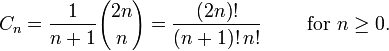
\includegraphics[scale=.6]{graphics/3bd4ac77a4af3f894d8e88ed7e1ba418.png}
% \caption{C\_n =
% \textbackslash{}frac\{1\}\{n+1\}\{2n\textbackslash{}choose n\} =
% \textbackslash{}frac\{(2n)!\}\{(n+1)!\textbackslash{},n!\}
% \textbackslash{}qquad\textbackslash{}mbox\{ for \}n\textbackslash{}ge
% 0.}
\end{figure}

Or recursively:

\begin{figure}[htbp]
\centering
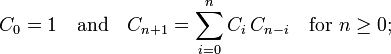
\includegraphics[scale=.6]{graphics/2f17435a71394ce667ab694b27341560.png}
% \caption{C\_0 = 1 \textbackslash{}quad \textbackslash{}mbox\{and\}
% \textbackslash{}quad
% C\_\{n+1\}=\textbackslash{}sum\_\{i=0\}\^{}\{n\}C\_i\textbackslash{},C\_\{n-i\}\textbackslash{}quad\textbackslash{}text\{for
% \}n\textbackslash{}ge 0;}
\end{figure}

Or alternatively (also recursive):

\begin{figure}[htbp]
\centering
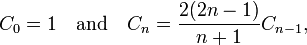
\includegraphics[scale=.6]{graphics/619a49e5557ce15be15ecd45dc767c72.png}
% \caption{C\_0 = 1 \textbackslash{}quad \textbackslash{}mbox\{and\}
% \textbackslash{}quad
% C\_n=\textbackslash{}frac\{2(2n-1)\}\{n+1\}C\_\{n-1\},}
\end{figure}

Implement at least one of these algorithms and print out the first 15
Catalan numbers with each. \emph{Memoization} is not
required, but may be worth the effort when using the second method
above.

\begin{description}
\item[Cf.]
\end{description}

\begin{itemize}
\item
  \emph{Pascal's triangle}
\item
  \href{http://milan.milanovic.org/math/english/fibo/fibo4.html}{Catalan
  Numbers and the Pascal Triangle}
\item
  \href{http://rosettacode.org/wiki/Catalan\_numbers\#An\_Alternative\_Approach}{http://rosettacode.org/wiki/Catalan\_numbers\#An\_Alternative\_Approach}
\end{itemize}


\begin{wideverbatim}

# Factorial
(de fact (N)
   (if (=0 N)
      1
      (* N (fact (dec N))) ) )

# Directly
(de catalanDir (N)
   (/ (fact (* 2 N)) (fact (inc N)) (fact N)) )

# Recursively
(de catalanRec (N)
   (if (=0 N)
      1
      (cache '(NIL) (pack (char (hash N)) N)  # Memoize
         (sum
            '((I) (* (catalanRec I) (catalanRec (- N I 1))))
            (range 0 (dec N)) ) ) ) )

# Alternatively
(de catalanAlt (N)
   (if (=0 N)
      1
      (*/ 2 (dec (* 2 N)) (catalanAlt (dec N)) (inc N)) ) )

# Test
(for (N 0 (> 15 N) (inc N))
   (tab (2 4 8 8 8)
      N
      " => "
      (catalanDir N)
      (catalanRec N)
      (catalanAlt N) ) )

Output:

 0 =>        1       1       1
 1 =>        1       1       1
 2 =>        2       2       2
 3 =>        5       5       5
 4 =>       14      14      14
 5 =>       42      42      42
 6 =>      132     132     132
 7 =>      429     429     429
 8 =>     1430    1430    1430
 9 =>     4862    4862    4862
10 =>    16796   16796   16796
11 =>    58786   58786   58786
12 =>   208012  208012  208012
13 =>   742900  742900  742900
14 =>  2674440 2674440 2674440

\end{wideverbatim}

\pagebreak{}
\section*{Character codes}

Given a character value in your language, print its code (could be ASCII
code, Unicode code, or whatever your language uses). For example, the
character `a' (lowercase letter A) has a code of 97 in ASCII (as well as
Unicode, as ASCII forms the beginning of Unicode). Conversely, given a
code, print out the corresponding character.


\begin{figure}[H]
  \centering
  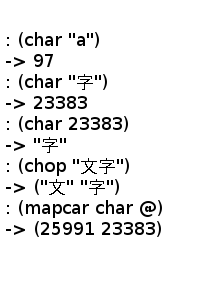
\includegraphics[scale=.6]{graphics/kanji.png}
\end{figure}

% \begin{CJK}{UTF8}{}
% \begin{Japanese}
% \noindent: (char ``a'') \\
% -> 97 \\
% : (char ``字'') \\
% -> 23383 \\
% : (char 23383) \\
% -> ``字'' \\
% : (chop ``文字'') \\
% -> (``文'' ``字'') \\
% : (mapcar char @) \\
% -> (25991 23383)
% \end{Japanese}
% \end{CJK}

% \begin{wideverbatim}

% : (char "a")
% -> 97
% : (char "字")
% -> 23383
% : (char 23383)
% -> "字"
% : (chop "文字")
% -> ("文" "字")
% : (mapcar char @)
% -> (25991 23383)

% \end{wideverbatim}

\pagebreak{}
\section*{Character matching}


\textbf{Basic Data Operation}\\ This is a basic data operation. It
represents a fundamental action on a basic data type.

You may see other such operations in the \emph{Basic Data Operations}
category, or:

\textbf{Integer Operations} \\
\emph{Arithmetic} \textbar{} \emph{Comparison}

\textbf{Boolean Operations} \\ \emph{Bitwise} \textbar{}
\emph{Logical}

\textbf{String Operations} \\
\emph{Concatenation} \textbar{} \emph{Interpolation} \textbar{}
\textbf{Matching}

\textbf{Memory Operations} \\
\emph{Pointers \& references} \textbar{} \emph{Addresses}

Given two strings, demonstrate the following 3 types of matchings:

\begin{enumerate}
\item
  Determining if the first string starts with second string
\item
  Determining if the first string contains the second string at any
  location
\item
  Determining if the first string ends with the second string
\end{enumerate}

Optional requirements:

\begin{enumerate}
\item
  Print the location of the match for part 2
\item
  Handle multiple occurrences of a string for part 2.
\end{enumerate}



\begin{wideverbatim}

: (pre? "ab" "abcd")
-> "abcd"
: (pre? "xy" "abcd")
-> NIL

: (sub? "bc" "abcd")
-> "abcd"
: (sub? "xy" "abcd")
-> NIL

: (tail (chop "cd") (chop "abcd"))
-> ("c" "d")
: (tail (chop "xy") (chop "abcd"))
-> NIL


(de positions (Pat Str)
   (setq Pat (chop Pat))
   (make
      (for ((I . L) (chop Str) L (cdr L))
         (and (head Pat L) (link I)) ) ) )

: (positions "bc" "abcdabcd")
-> (2 6)

\end{wideverbatim}

\pagebreak{}
\section*{Chat server}

Write a server for a minimal text based chat. People should be able to
connect via `telnet', sign on with a nickname, and type messages which
will then be seen by all other connected users. Arrivals and departures
of chat members should generate appropriate notification messages.



\begin{wideverbatim}

#!/usr/bin/picolisp /usr/lib/picolisp/lib.l
 
(de chat Lst
   (out *Sock
      (mapc prin Lst)
      (prinl) ) )
 
(setq *Port (port 4004))
 
(loop
   (setq *Sock (listen *Port))
   (NIL (fork) (close *Port))
   (close *Sock) )
 
(out *Sock
   (prin "Please enter your name: ")
   (flush) )
(in *Sock (setq *Name (line T)))
 
(tell 'chat "+++ " *Name " arrived +++")
 
(task *Sock
   (in @
      (ifn (eof)
         (tell 'chat *Name "> " (line T))
         (tell 'chat "--- " *Name " left ---")
         (bye) ) ) )
(wait)

\end{wideverbatim}

\begin{wideverbatim}

Output:

After starting the above script, connect to the chat server from two terminals:

           Terminal 1            |           Terminal 2
---------------------------------+---------------------------------
\$ telnet localhost 4004         |
Trying ::1...                    |
Trying 127.0.0.1...              |
Connected to localhost.          |
Escape character is '^]'.        |
Please enter your name: Ben      |
                                 | \$ telnet localhost 4004
                                 | Trying ::1...
                                 | Trying 127.0.0.1...
                                 | Connected to localhost.
                                 | Escape character is '^]'.
                                 | Please enter your name: Tom
+++ Tom arrived +++              |
Hi Tom                           |
                                 | Ben> Hi Tom
                                 | Hi Ben
Tom> Hi Ben                      |
                                 | How are you?
Tom> How are you?                |
Thanks, fine!                    |
                                 | Ben> Thanks, fine!
                                 | See you!
Tom> See you!                    |
                                 | ^]
                                 | telnet> quit
--- Tom left ---                 |
                                 | Connection closed.
                                 | \$

\end{wideverbatim}

\pagebreak{}
\section*{Checkpoint synchronization}

The checkpoint synchronization is a problem of synchronizing multiple
\emph{tasks}. Consider a workshop where several workers (\emph{tasks})
assembly details of some mechanism. When each of them completes his
work they put the details together. There is no store, so a worker who
finished its part first must wait for others before starting another
one. Putting details together is the \emph{checkpoint} at which
\emph{tasks} synchronize themselves before going their paths apart.

\textbf{The task}

Implement checkpoint synchronization in your language.

Make sure that the solution is \emph{race condition}-free. Note that a
straightforward solution based on \emph{events} is exposed to
\emph{race condition}. Let two \emph{tasks} A and B need to be
synchronized at a checkpoint. Each signals its event (\emph{EA} and
\emph{EB} correspondingly), then waits for the AND-combination of the
events (\emph{EA}\&\emph{EB}) and resets its event. Consider the
following scenario: A signals \emph{EA} first and gets blocked waiting
for \emph{EA}\&\emph{EB}. Then B signals \emph{EB} and loses the
processor. Then A is released (both events are signaled) and resets
\emph{EA}. Now if B returns and enters waiting for
\emph{EA}\&\emph{EB}, it gets lost.

When a worker is ready it shall not continue before others finish. A
typical implementation bug is when a worker is counted twice within one
working cycle causing its premature completion. This happens when the
quickest worker serves its cycle two times while the laziest one is
lagging behind.

If you can, implement workers joining and leaving.

\begin{wideverbatim}

The following solution implements each worker as a coroutine. Therefore, it
works only in the 64-bit version.

'checkpoints' takes a number of projects to do, and a number of workers. Each
worker is started with a random number of steps to do (between 2 and 5), and is
kept in a list of 'Staff' members. Whenever a worker finishes, he is removed
from that list, until it is empty and the project is done.

'worker' takes a number of steps to perform. It "works" by printing each step,
and returning NIL when done.

(de checkpoints (Projects Workers)
   (for P Projects
      (prinl "Starting project number " P ":")
      (for
         (Staff
            (mapcar
               '((I) (worker (format I) (rand 2 5)))  # Create staff of workers
               (range 1 Workers) )
            Staff                                     # While still busy
            (filter worker Staff) ) )                 # Remove finished workers
      (prinl "Project number " P " is done.") ) )

(de worker (ID Steps)
   (co ID
      (prinl "Worker " ID " has " Steps " steps to do")
      (for N Steps
         (yield ID)
         (prinl "Worker " ID " step " N) )
      NIL ) )

\end{wideverbatim}

\begin{wideverbatim}

Output:

: (checkpoints 2 3)  # Start two projects with 3 workers
Starting project number 1:
Worker 1 has 2 steps to do
Worker 2 has 3 steps to do
Worker 3 has 5 steps to do
Worker 1 step 1
Worker 2 step 1
Worker 3 step 1
Worker 1 step 2
Worker 2 step 2
Worker 3 step 2
Worker 2 step 3
Worker 3 step 3
Worker 3 step 4
Worker 3 step 5
Project number 1 is done.
Starting project number 2:
Worker 1 has 4 steps to do
Worker 2 has 3 steps to do
Worker 3 has 2 steps to do
Worker 1 step 1
Worker 2 step 1
Worker 3 step 1
Worker 1 step 2
Worker 2 step 2
Worker 3 step 2
Worker 1 step 3
Worker 2 step 3
Worker 1 step 4
Project number 2 is done.

\end{wideverbatim}

\pagebreak{}
\section*{Chess player}

In the early times, chess used to be the prime example of artificial
intelligence. Nowadays, some chess programs can beat a human master, and
simple implementations can be written in a few pages of code.

Write a program which plays chess against a human player. No need for
graphics -- a textual user interface is sufficient.

\begin{wideverbatim}

See [[Chess player/PicoLisp]].

This implementation supports all chess rules (including castling, pawn promotion
and en passant), switching sides, unlimited undo/redo, and the setup, saving and
loading of board positions to/from files.


# *Board a1 .. h8
# *White *Black *WKPos *BKPos *Pinned
# *Depth *Moved *Undo *Redo *Me *You
 
(load "@lib/simul.l")

### Fields/Board ###
# x y color piece whAtt blAtt
 
(setq *Board (grid 8 8))
 
(for (X . Lst) *Board
   (for (Y . This) Lst
      (=: x X)
      (=: y Y)
      (=: color (not (bit? 1 (+ X Y)))) ) )
 
(de *Straight `west `east `south `north)
 
(de *Diagonal
   ((This) (: 0 1  1  0 -1  1))   # Southwest
   ((This) (: 0 1  1  0 -1 -1))   # Northwest
   ((This) (: 0 1 -1  0 -1  1))   # Southeast
   ((This) (: 0 1 -1  0 -1 -1)) ) # Northeast
 
(de *DiaStraight
   ((This) (: 0 1  1  0 -1  1  0 -1  1))   # South Southwest
   ((This) (: 0 1  1  0 -1  1  0  1  1))   # West Southwest
   ((This) (: 0 1  1  0 -1 -1  0  1  1))   # West Northwest
   ((This) (: 0 1  1  0 -1 -1  0 -1 -1))   # North Northwest
   ((This) (: 0 1 -1  0 -1 -1  0 -1 -1))   # North Northeast
   ((This) (: 0 1 -1  0 -1 -1  0  1 -1))   # East Northeast
   ((This) (: 0 1 -1  0 -1  1  0  1 -1))   # East Southeast
   ((This) (: 0 1 -1  0 -1  1  0 -1  1)) ) # South Southeast
 

\end{wideverbatim}

\begin{wideverbatim}
 
### Pieces ###
(de piece (Typ Cnt Fld)
   (prog1
      (def
         (pack (mapcar '((Cls) (cdr (chop Cls))) Typ))
         Typ )
      (init> @ Cnt Fld) ) )
 
 
(class +White)
# color ahead
 
(dm init> (Cnt Fld)
   (=: ahead north)
   (extra Cnt Fld) )
 
(dm name> ()
   (pack " " (extra) " ") )
 
(dm move> (Fld)
   (adjMove '*White '*WKPos whAtt- whAtt+) )
 
 
(class +Black)
# color ahead
 
(dm init> (Cnt Fld)
   (=: color T)
   (=: ahead south)
   (extra Cnt Fld) )
 
(dm name> ()
   (pack '< (extra) '>) )
 
(dm move> (Fld)
   (adjMove '*Black '*BKPos blAtt- blAtt+) )
 
 
(class +piece)
# cnt field attacks
 
(dm init> (Cnt Fld)
   (=: cnt Cnt)
   (move> This Fld) )
 
(dm ctl> ())
 

\end{wideverbatim}

\begin{wideverbatim}

 
(class +King +piece)
 
(dm name> () 'K)
 
(dm val> () 120)
 
(dm ctl> ()
   (unless (=0 (: cnt)) -10) )
 
(dm moves> ()
   (make
      (unless
         (or
            (n0 (: cnt))
            (get (: field) (if (: color) 'whAtt 'blAtt)) )
         (tryCastle west T)
         (tryCastle east) )
      (try1Move *Straight)
      (try1Move *Diagonal) ) )
 
(dm attacks> ()
   (make
      (try1Attack *Straight)
      (try1Attack *Diagonal) ) )
 
 
(class +Castled)
 
(dm ctl> () 30)
 
 
(class +Queen +piece)
 
(dm name> () 'Q)
 
(dm val> () 90)
 
(dm moves> ()
   (make
      (tryMoves *Straight)
      (tryMoves *Diagonal) ) )
 
(dm attacks> ()
   (make
      (tryAttacks *Straight)
      (tryAttacks *Diagonal T) ) )
 

\end{wideverbatim}

\begin{wideverbatim}

 
(class +Rook +piece)
 
(dm name> () 'R)
 
(dm val> () 47)
 
(dm moves> ()
   (make (tryMoves *Straight)) )
 
(dm attacks> ()
   (make (tryAttacks *Straight)) )
 
 
(class +Bishop +piece)
 
(dm name> () 'B)
 
(dm val> () 33)
 
(dm ctl> ()
   (when (=0 (: cnt)) -10) )
 
(dm moves> ()
   (make (tryMoves *Diagonal)) )
 
(dm attacks> ()
   (make (tryAttacks *Diagonal T)) )
 
 
(class +Knight +piece)
 
(dm name> () 'N)
 
(dm val> () 28)
 
(dm ctl> ()
   (when (=0 (: cnt)) -10) )
 
(dm moves> ()
   (make (try1Move *DiaStraight)) )
 
(dm attacks> ()
   (make (try1Attack *DiaStraight)) )


\end{wideverbatim}

\begin{wideverbatim}
 
 
(class +Pawn +piece)
 
(dm name> () 'P)
 
(dm val> () 10)
 
(dm moves> ()
   (let (Fld1 ((: ahead) (: field))  Fld2 ((: ahead) Fld1))
      (make
         (and
            (tryPawnMove Fld1 Fld2)
            (=0 (: cnt))
            (tryPawnMove Fld2 T) )
         (tryPawnCapt (west Fld1) Fld2 (west (: field)))
         (tryPawnCapt (east Fld1) Fld2 (east (: field))) ) ) )
 
(dm attacks> ()
   (let Fld ((: ahead) (: field))
      (make
         (and (west Fld) (link @))
         (and (east Fld) (link @)) ) ) )
 

\end{wideverbatim}

\begin{wideverbatim}
 
### Move Logic ###
(de inCheck (Color)
   (if Color (get *BKPos 'whAtt) (get *WKPos 'blAtt)) )
 
(de whAtt+ (This Pce)
   (=: whAtt (cons Pce (: whAtt))) )
 
(de whAtt- (This Pce)
   (=: whAtt (delq Pce (: whAtt))) )
 
(de blAtt+ (This Pce)
   (=: blAtt (cons Pce (: blAtt))) )
 
(de blAtt- (This Pce)
   (=: blAtt (delq Pce (: blAtt))) )
 
(de adjMove (Var KPos Att- Att+)
   (let (W (: field whAtt)  B (: field blAtt))
      (when (: field)
         (put @ 'piece NIL)
         (for F (: attacks) (Att- F This)) )
      (nond
         (Fld (set Var (delq This (val Var))))
         ((: field) (push Var This)) )
      (ifn (=: field Fld)
         (=: attacks)
         (put Fld 'piece This)
         (and (isa '+King This) (set KPos Fld))
         (for F (=: attacks (attacks> This)) (Att+ F This)) )
      (reAtttack W (: field whAtt) B (: field blAtt)) ) )
 
(de reAtttack (W W2 B B2)
   (for This W
      (unless (memq This W2)
         (for F (: attacks) (whAtt- F This))
         (for F (=: attacks (attacks> This)) (whAtt+ F This)) ) )
   (for This W2
      (for F (: attacks) (whAtt- F This))
      (for F (=: attacks (attacks> This)) (whAtt+ F This)) )
   (for This B
      (unless (memq This B2)
         (for F (: attacks) (blAtt- F This))
         (for F (=: attacks (attacks> This)) (blAtt+ F This)) ) )
   (for This B2
      (for F (: attacks) (blAtt- F This))
      (for F (=: attacks (attacks> This)) (blAtt+ F This)) ) )


\end{wideverbatim}

\begin{wideverbatim}

 
(de try1Move (Lst)
   (for Dir Lst
      (let? Fld (Dir (: field))
         (ifn (get Fld 'piece)
            (link (list This (cons This Fld)))
            (unless (== (: color) (get @ 'color))
               (link
                  (list This
                     (cons (get Fld 'piece))
                     (cons This Fld) ) ) ) ) ) ) )
 
(de try1Attack (Lst)
   (for Dir Lst
      (and (Dir (: field)) (link @)) )  )
 
(de tryMoves (Lst)
   (for Dir Lst
      (let Fld (: field)
         (loop
            (NIL (setq Fld (Dir Fld)))
            (T (get Fld 'piece)
               (unless (== (: color) (get @ 'color))
                  (link
                     (list This
                        (cons (get Fld 'piece))
                        (cons This Fld) ) ) ) )
            (link (list This (cons This Fld))) ) ) ) )
 
(de tryAttacks (Lst Diag)
   (use (Pce Cls Fld2)
      (for Dir Lst
         (let Fld (: field)
            (loop
               (NIL (setq Fld (Dir Fld)))
               (link Fld)
               (T
                  (and
                     (setq Pce (get Fld 'piece))
                     (<> (: color) (get Pce 'color)) ) )
               (T (== '+Pawn (setq Cls (last (type Pce))))
                  (and
                     Diag
                     (setq Fld2 (Dir Fld))
                     (= (get Fld2 'y) (get ((get Pce 'ahead) Fld) 'y))
                     (link Fld2) ) )
               (T (memq Cls '(+Knight +Queen +King)))
               (T (and Pce (xor Diag (== Cls '+Bishop)))) ) ) ) ) )



\end{wideverbatim}

\begin{wideverbatim}

 
(de tryPawnMove (Fld Flg)
   (unless (get Fld 'piece)
      (if Flg
         (link (list This (cons This Fld)))
         (for Cls '(+Queen +Knight +Rook +Bishop)
            (link
               (list This
                  (cons This)
                  (cons
                     (piece (list (car (type This)) Cls) (: cnt))
                     Fld ) ) ) ) ) ) )
 
(de tryPawnCapt (Fld1 Flg Fld2)
   (if (get Fld1 'piece)
      (unless (== (: color) (get @ 'color))
         (if Flg
            (link
               (list This
                  (cons (get Fld1 'piece))
                  (cons This Fld1) ) )
            (for Cls '(+Queen +Knight +Rook +Bishop)
               (link
                  (list This
                     (cons (get Fld1 'piece))
                     (cons This)
                     (cons
                        (piece (list (car (type This)) Cls) (: cnt))
                        Fld1 ) ) ) ) ) )
      (let? Pce (get Fld2 'piece)
         (and
            (== Pce (car *Moved))
            (= 1 (get Pce 'cnt))
            (isa '+Pawn Pce)
            (n== (: color) (get Pce 'color))
            (link (list This (cons Pce) (cons This Fld1))) ) ) ) )


\end{wideverbatim}

\begin{wideverbatim}
 
(de tryCastle (Dir Long)
   (use (Fld1 Fld2 Fld Pce)
      (or
         (get (setq Fld1 (Dir (: field))) 'piece)
         (get Fld1 (if (: color) 'whAtt 'blAtt))
         (get (setq Fld2 (Dir Fld1)  Fld Fld2) 'piece)
         (when Long
            (or
               (get (setq Fld (Dir Fld)) 'piece)
               (get Fld (if (: color) 'whAtt 'blAtt)) ) )
         (and
            (== '+Rook (last (type (setq Pce (get (Dir Fld) 'piece)))))
            (=0 (get Pce 'cnt))
            (link
               (list This
                  (cons This)
                  (cons
                     (piece (cons (car (type This)) '(+Castled +King)) 1)
                     Fld2 )
                  (cons Pce Fld1) ) ) ) ) ) )

(de pinned (Fld Lst Color)
   (use (Pce L P)
      (and
         (loop
            (NIL (setq Fld (Dir Fld)))
            (T (setq Pce (get Fld 'piece))
               (and
                  (= Color (get Pce 'color))
                  (setq L
                     (make
                        (loop
                           (NIL (setq Fld (Dir Fld)))
                           (link Fld)
                           (T (setq P (get Fld 'piece))) ) ) )
                  (<> Color (get P 'color))
                  (memq (last (type P)) Lst)
                  (cons Pce L) ) ) )
         (link @) ) ) )
 


\end{wideverbatim}

\begin{wideverbatim}

 
### Moves ###
# Move      ((p1 (p1 . f2))        . ((p1 . f1)))
# Capture   ((p1 (p2) (p1 . f2))   . ((p1 . f1) (p2 . f2)))
# Castle    ((K (K) (C . f2) (R . f4)) . ((R . f3) (K . f1)))
# Promote   ((P (P) (Q . f2))      . ((Q) (P . f1)))
# Capt/Prom ((P (p1) (P) (Q . f2)) . ((Q) (P . f1) (p1 . f2)))
(de moves (Color)
   (filter
      '((Lst)
         (prog2
            (move (car Lst))
            (not (inCheck Color))
            (move (cdr Lst)) ) )
      (mapcan
         '((Pce)
            (mapcar
               '((Lst)
                  (cons Lst
                     (flip
                        (mapcar
                           '((Mov) (cons (car Mov) (get Mov 1 'field)))
                           (cdr Lst) ) ) ) )
               (moves> Pce) ) )
         (if Color *Black *White) ) ) )
 
(de move (Lst)
   (if (atom (car Lst))
      (inc (prop (push '*Moved (pop 'Lst)) 'cnt))
      (dec (prop (pop '*Moved) 'cnt)) )
   (for Mov Lst
      (move> (car Mov) (cdr Mov)) ) )
 

\end{wideverbatim}

\begin{wideverbatim}

 
### Evaluation ###
(de mate (Color)
   (and (inCheck Color) (not (moves Color))) )
 
(de battle (Fld Prey Attacker Defender)
   (use Pce
      (loop
         (NIL (setq Pce (mini 'val> Attacker)) 0)
         (setq Attacker (delq Pce Attacker))
         (NIL (and (asoq Pce *Pinned) (not (memq Fld @)))
            (max 0 (- Prey (battle Fld (val> Pce) Defender Attacker))) ) ) ) )
 
# Ref. Sargon, Dan and Kate Spracklen, Hayden 1978
(de cost (Color)
   (if (mate (not Color))
      -9999
      (setq *Pinned
         (make
            (for Dir *Straight
               (pinned *WKPos '(+Rook +Queen))
               (pinned *BKPos '(+Rook +Queen) T) )
            (for Dir *Diagonal
               (pinned *WKPos '(+Bishop +Queen))
               (pinned *BKPos '(+Bishop +Queen) T) ) ) )
      (let (Ctl 0  Mat 0  Lose 0  Win1 NIL  Win2 NIL  Flg NIL)
         (use (White Black Col Same B)
            (for Lst *Board
               (for This Lst
                  (setq White (: whAtt)  Black (: blAtt))
                  ((if Color inc dec) 'Ctl (- (length White) (length Black)))
                  (let? Val (and (: piece) (val> @))
                     (setq Col (: piece color)  Same (== Col Color))
                     ((if Same dec inc) 'Ctl (ctl> (: piece)))
                     (unless
                        (=0
                           (setq B
                              (if Col
                                 (battle This Val White Black)
                                 (battle This Val Black White) ) ) )
                        (dec 'Val 5)
                        (if Same
                           (setq
                              Lose (max Lose B)
                              Flg (or Flg (== (: piece) (car *Moved))) )
                           (when (> B Win1)
                              (xchg 'B 'Win1)
                              (setq Win2 (max Win2 B)) ) ) )
                     ((if Same dec inc) 'Mat Val) ) ) ) )
         (unless (=0 Lose) (dec 'Lose 5))
         (if Flg
            (* 4 (+ Mat Lose))
            (when Win2
               (dec 'Lose (>> 1 (- Win2 5))) )
            (+ Ctl (* 4 (+ Mat Lose))) ) ) ) )

\end{wideverbatim}

\begin{wideverbatim}
 
### Game ###
(de display (Res)
   (when Res
      (disp *Board T
         '((This)
            (cond
               ((: piece) (name> @))
               ((: color) " - ")
               (T "   ") ) ) ) )
   (and (inCheck *You) (prinl "(+)"))
   Res )
 
(de moved? (Lst)
   (or
      (> 16 (length Lst))
      (find '((This) (n0 (: cnt))) Lst) ) )
 
(de bookMove (From To)
   (let Pce (get From 'piece)
      (list 0 (list (list Pce (cons Pce To)) (cons Pce From))) ) )
 
(de myMove ()
   (let? M
      (cadr
         (cond
            ((moved? (if *Me *Black *White))
               (game *Me *Depth moves move cost) )
            (*Me
               (if (member (get *Moved 1 'field 'x) (1 2 3 5))
                  (bookMove 'e7 'e5)
                  (bookMove 'd7 'd5) ) )
            ((rand T) (bookMove 'e2 'e4))
            (T (bookMove 'd2 'd4)) ) )
      (move (car (push '*Undo M)))
      (off *Redo)
      (cons
         (caar M)
         (cdr (asoq (caar M) (cdr M)))
         (pick cdr (cdar M)) ) ) )


\end{wideverbatim}

\begin{wideverbatim}

 
(de yourMove (From To Cls)
   (when
      (find
         '((Mov)
            (and
               (== (caar Mov) (get From 'piece))
               (== To (pick cdr (cdar Mov)))
               (or
                  (not Cls)
                  (isa Cls (car (last (car Mov)))) ) ) )
         (moves *You) )
      (prog1 (car (push '*Undo @))
         (off *Redo)
         (move @) ) ) )
 
(de undo ()
   (move (cdr (push '*Redo (pop '*Undo)))) )
 
(de redo ()
   (move (car (push '*Undo (pop '*Redo)))) )
 
(de setup (Depth You Init)
   (setq *Depth (or Depth 5)  *You You  *Me (not You))
   (off *White *Black *Moved *Undo *Redo)
   (for Lst *Board
      (for This Lst (=: piece) (=: whAtt) (=: blAtt)) )
   (if Init
      (for L Init
         (with (piece (cadr L) 0 (car L))
            (unless (caddr L)
               (=: cnt 1)
               (push '*Moved This) ) ) )
      (mapc
         '((Cls Lst)
            (piece (list '+White Cls) 0 (car Lst))
            (piece '(+White +Pawn) 0 (cadr Lst))
            (piece '(+Black +Pawn) 0 (get Lst 7))
            (piece (list '+Black Cls) 0 (get Lst 8)) )
         '(+Rook +Knight +Bishop +Queen +King +Bishop +Knight +Rook)
         *Board ) ) )


\end{wideverbatim}

\begin{wideverbatim}

 
(de main (Depth You Init)
   (setup Depth You Init)
   (display T) )
 
(de go Args
   (display
      (cond
         ((not Args) (xchg '*Me '*You) (myMove))
         ((== '- (car Args)) (and *Undo (undo)))
         ((== '+ (car Args)) (and *Redo (redo)))
         ((apply yourMove Args) (display T) (myMove)) ) ) )
 
# Print position to file
(de ppos (File)
   (out File
      (println
         (list 'main *Depth *You
            (lit
               (mapcar
                  '((This)
                     (list
                        (: field)
                        (val This)
                        (not (memq This *Moved)) ) )
                  (append *White *Black) ) ) ) ) ) )



\end{wideverbatim}

\begin{wideverbatim}


Start:

\$ pil chess.l -main +
   +---+---+---+---+---+---+---+---+
 8 |<R>|<N>|<B>|<Q>|<K>|<B>|<N>|<R>|
   +---+---+---+---+---+---+---+---+
 7 |<P>|<P>|<P>|<P>|<P>|<P>|<P>|<P>|
   +---+---+---+---+---+---+---+---+
 6 |   | - |   | - |   | - |   | - |
   +---+---+---+---+---+---+---+---+
 5 | - |   | - |   | - |   | - |   |
   +---+---+---+---+---+---+---+---+
 4 |   | - |   | - |   | - |   | - |
   +---+---+---+---+---+---+---+---+
 3 | - |   | - |   | - |   | - |   |
   +---+---+---+---+---+---+---+---+
 2 | P | P | P | P | P | P | P | P |
   +---+---+---+---+---+---+---+---+
 1 | R | N | B | Q | K | B | N | R |
   +---+---+---+---+---+---+---+---+
     a   b   c   d   e   f   g   h


\end{wideverbatim}

\begin{wideverbatim}

Entering moves:

: (go e2 e4)

Undo moves:

: (go -)

Redo:

: (go +)

Switch sides:

: (go)

Save position to a file:

: (ppos "file")

Load position from file:

: (load "file")

\end{wideverbatim}

\pagebreak{}
\section*{Cholesky decomposition}


Every symmetric, positive definite matrix A can be decomposed into a
product of a unique lower triangular matrix L and its transpose:

\emph{A} = \emph{L}\emph{L}\textsuperscript{\emph{T}}

\emph{L} is called- the \emph{Cholesky factor} of \emph{A}, and can be
interpreted as a generalized square root of \emph{A}, as described in
\href{http://en.wikipedia.org/wiki/Cholesky\_decomposition}{Cholesky
decomposition}.

In a 3x3 example, we have to solve the following system of equations:

\begin{figure}[H]
\centering
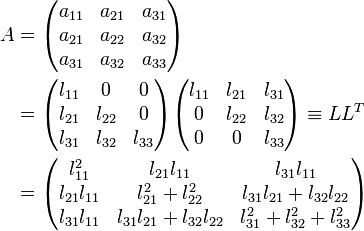
\includegraphics[scale=.6]{graphics/d9fa28df063d00917f713bd9de134ad5.png}
% \caption{\textbackslash{}begin\{align\} A \&=
% \textbackslash{}begin\{pmatrix\} a\_\{11\} \& a\_\{21\} \&
% a\_\{31\}\textbackslash{}\textbackslash{} a\_\{21\} \& a\_\{22\} \&
% a\_\{32\}\textbackslash{}\textbackslash{} a\_\{31\} \& a\_\{32\} \&
% a\_\{33\}\textbackslash{}\textbackslash{}
% \textbackslash{}end\{pmatrix\}\textbackslash{}\textbackslash{} \& =
% \textbackslash{}begin\{pmatrix\} l\_\{11\} \& 0 \& 0
% \textbackslash{}\textbackslash{} l\_\{21\} \& l\_\{22\} \& 0
% \textbackslash{}\textbackslash{} l\_\{31\} \& l\_\{32\} \&
% l\_\{33\}\textbackslash{}\textbackslash{} \textbackslash{}end\{pmatrix\}
% \textbackslash{}begin\{pmatrix\} l\_\{11\} \& l\_\{21\} \& l\_\{31\}
% \textbackslash{}\textbackslash{} 0 \& l\_\{22\} \& l\_\{32\}
% \textbackslash{}\textbackslash{} 0 \& 0 \& l\_\{33\}
% \textbackslash{}end\{pmatrix\} \textbackslash{}equiv
% LL\^{}T\textbackslash{}\textbackslash{} \&=
% \textbackslash{}begin\{pmatrix\} l\_\{11\}\^{}2 \& l\_\{21\}l\_\{11\} \&
% l\_\{31\}l\_\{11\} \textbackslash{}\textbackslash{} l\_\{21\}l\_\{11\}
% \& l\_\{21\}\^{}2 + l\_\{22\}\^{}2\&
% l\_\{31\}l\_\{21\}+l\_\{32\}l\_\{22\} \textbackslash{}\textbackslash{}
% l\_\{31\}l\_\{11\} \& l\_\{31\}l\_\{21\}+l\_\{32\}l\_\{22\} \&
% l\_\{31\}\^{}2 + l\_\{32\}\^{}2+l\_\{33\}\^{}2
% \textbackslash{}end\{pmatrix\}\textbackslash{}end\{align\} }
\end{figure}

We can see that for the diagonal elements
(\emph{l}\textsubscript{\emph{k}\emph{k}}) of \emph{L} there is a
calculation pattern:

\begin{figure}[H]
\centering
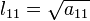
\includegraphics[scale=.6]{graphics/409b5a2625bed1a4a6c798323ae1db78.png}
% \caption{l\_\{11\} = \textbackslash{}sqrt\{a\_\{11\}\}}
\end{figure}

\begin{figure}[H]
\centering
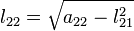
\includegraphics[scale=.6]{graphics/2cf603737e11dad8ec4d00dc8298c639.png}
% \caption{l\_\{22\} = \textbackslash{}sqrt\{a\_\{22\} - l\_\{21\}\^{}2\}}
\end{figure}

\begin{figure}[H]
\centering
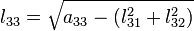
\includegraphics[scale=.6]{graphics/385714f276153424a4447fa0ede31bf4.png}
% \caption{l\_\{33\} = \textbackslash{}sqrt\{a\_\{33\} - (l\_\{31\}\^{}2 +
% l\_\{32\}\^{}2)\}}
\end{figure}

or in general:

\begin{figure}[H]
\centering
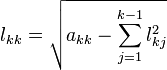
\includegraphics[scale=.6]{graphics/af307c5e65e7403b785f8a2c6b9d051a.png}
% \caption{l\_\{kk\} = \textbackslash{}sqrt\{a\_\{kk\} -
% \textbackslash{}sum\_\{j=1\}\^{}\{k-1\} l\_\{kj\}\^{}2\}}
\end{figure}

For the elements below the diagonal
(\emph{l}\textsubscript{\emph{i}\emph{k}}, where \emph{i} \textgreater{}
\emph{k}) there is also a calculation pattern:

\begin{figure}[H]
\centering
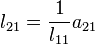
\includegraphics[scale=.6]{graphics/91035139969200d1af754ee0d07acd6a.png}
% \caption{l\_\{21\} = \textbackslash{}frac\{1\}\{l\_\{11\}\} a\_\{21\}}
\end{figure}

\begin{figure}[H]
\centering
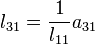
\includegraphics[scale=.6]{graphics/bdd8a535c6a8470767849ade18412c6d.png}
% \caption{l\_\{31\} = \textbackslash{}frac\{1\}\{l\_\{11\}\} a\_\{31\}}
\end{figure}

\begin{figure}[H]
\centering
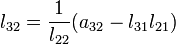
\includegraphics[scale=.6]{graphics/8c7f6df9ddc2c13f56a13ca113710587.png}
% \caption{l\_\{32\} = \textbackslash{}frac\{1\}\{l\_\{22\}\} (a\_\{32\} -
% l\_\{31\}l\_\{21\})}
\end{figure}

which can also be expressed in a general formula:

\begin{figure}[H]
\centering
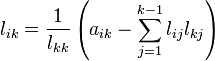
\includegraphics[scale=.6]{graphics/a404f9cdcc88e086294f604a41599f92.png}
% \caption{l\_\{ik\} = \textbackslash{}frac\{1\}\{l\_\{kk\}\}
% \textbackslash{}left ( a\_\{ik\} -
% \textbackslash{}sum\_\{j=1\}\^{}\{k-1\} l\_\{ij\}l\_\{kj\}
% \textbackslash{}right )}
\end{figure}

\textbf{Task description}

The task is to implement a routine which will return a lower Cholesky
factor \emph{L} for every given symmetric, positive definite nxn matrix
\emph{A}. You should then test it on the following two examples and
include your output.

Example 1:

\begin{wideverbatim}
25  15  -5                 5   0   0
15  18   0         -->     3   3   0
-5   0  11                -1   1   3
\end{wideverbatim}

Example 2:

\begin{wideverbatim}
18  22   54   42           4.24264    0.00000    0.00000    0.00000
22  70   86   62   -->     5.18545    6.56591    0.00000    0.00000
54  86  174  134          12.72792    3.04604    1.64974    0.00000
42  62  134  106           9.89949    1.62455    1.84971    1.39262
\end{wideverbatim}


\begin{wideverbatim}

(scl 9)
(load "@lib/math.l")

(de cholesky (A)
   (let L (mapcar '(() (need (length A) 0)) A)
      (for (I . R) A
         (for J I
            (let S (get R J)
               (for K (inc J)
                  (dec 'S (*/ (get L I K) (get L J K) 1.0)) )
               (set (nth L I J)
                  (if (= I J)
                     (sqrt (* 1.0 S))
                     (*/ S 1.0 (get L J J)) ) ) ) ) )
      (for R L
         (for N R (prin (align 9 (round N 5))))
         (prinl) ) ) )

Test:

(cholesky
   '((25.0 15.0 -5.0) (15.0 18.0 0) (-5.0 0 11.0)) )

(prinl)

(cholesky
   (quote
      (18.0  22.0   54.0   42.0)
      (22.0  70.0   86.0   62.0)
      (54.0  86.0  174.0  134.0)
      (42.0  62.0  134.0  106.0) ) )

Output:

  5.00000  0.00000  0.00000
  3.00000  3.00000  0.00000
 -1.00000  1.00000  3.00000

  4.24264  0.00000  0.00000  0.00000
  5.18545  6.56591  0.00000  0.00000
 12.72792  3.04604  1.64974  0.00000
  9.89949  1.62455  1.84971  1.39262

\end{wideverbatim}

\pagebreak{}
\section*{Classes}


In \emph{object-oriented programming} \textbf{class} is a set (a
\href{http://en.wikipedia.org/wiki/Transitive\_closure}{transitive
  closure}) of types bound by the relation of \emph{inheritance}. It
is said that all types derived from some base type T and the type T
itself form a class T. The first type T from the class T sometimes is
called the \textbf{root type} of the class.

A class of types itself, as a type, has the values and operations of
its own. The operations of are usually called \textbf{methods} of the
root type. Both operations and values are called \emph{polymorphic}.

A polymorphic operation (method) selects an implementation depending on
the actual specific type of the polymorphic argument. The action of
choice the type-specific implementation of a polymorphic operation is
called \textbf{dispatch}. Correspondingly, polymorphic operations are
often called \textbf{dispatching} or \textbf{virtual}. Operations with
multiple arguments and/or the results of the class are called
\textbf{multi-methods}. A further generalization of is the operation
with arguments and/or results from different classes.

\begin{itemize}
\item
  single-dispatch languages are those that allow only one argument or
  result to control the dispatch. Usually it is the first parameter,
  often hidden, so that a prefix notation \emph{x}.\emph{f}() is used
  instead of mathematical \emph{f}(\emph{x}).
\item
  multiple-dispatch languages allow many arguments and/or results to
  control the dispatch.
\end{itemize}

A polymorphic value has a type tag indicating its specific type from the
class and the corresponding specific value of that type. This type is
sometimes called \textbf{the most specific type} of a {[}polymorphic{]}
value. The type tag of the value is used in order to resolve the
dispatch. The set of polymorphic values of a class is a transitive
closure of the sets of values of all types from that class.

In many \emph{OO} languages the type of the class of T and T itself
are considered equivalent. In some languages they are distinct (like
in \emph{Ada}). When class T and T are equivalent, there is no way to
distinguish polymorphic and specific values.

The purpose of this task is to create a basic class with a method, a
constructor, an instance variable and how to instantiate it.


\begin{wideverbatim}

(class +Rectangle)
# dx dy

(dm area> ()  # Define a a method that calculates the rectangle's area
   (* (: dx) (: dy)) )

(println  # Create a rectangle, and print its area
   (area> (new '(+Rectangle) 'dx 3 'dy 4)) )

\end{wideverbatim}

\pagebreak{}
\section*{Closest-pair problem}

The aim of this task is to provide a function to find the closest two
points among a set of given points in two dimensions, i.e. to solve the
\href{http://en.wikipedia.org/wiki/Closest\_pair\_of\_points\_problem}{Closest
pair of points problem} in the \emph{planar} case.

The straightforward solution is a O(n\textsuperscript{2}) algorithm
(which we can call \emph{brute-force algorithm}); the pseudocode (using
indexes) could be simply:

\begin{wideverbatim}
bruteForceClosestPair of P(1), P(2), ... P(N)
if N < 2 then
  return ∞
else
  minDistance ← |P(1) - P(2)|
  minPoints ← { P(1), P(2) }
  foreach i ∈ [1, N-1]
    foreach j ∈ [i+1, N]
      if |P(i) - P(j)| < minDistance then
        minDistance ← |P(i) - P(j)|
        minPoints ← { P(i), P(j) } 
      endif
    endfor
  endfor
  return minDistance, minPoints
 endif
\end{wideverbatim}

A better algorithm is based on the recursive divide\&conquer approach,
as explained also at
\href{http://en.wikipedia.org/wiki/Closest\_pair\_of\_points\_problem\#Planar\_case}{Wikipedia},
which is O(\emph{n} log \emph{n}); a pseudocode could be:

\begin{wideverbatim}
closestPair of (xP, yP)
               where xP is P(1) .. P(N) sorted by x coordinate, and
                     yP is P(1) .. P(N) sorted by y coordinate (ascending order)
if N ≤ 3 then
  return closest points of xP using brute-force algorithm
else
  xL ← points of xP from 1 to ⌈N/2⌉
  xR ← points of xP from ⌈N/2⌉+1 to N
  xm ← xP(⌈N/2⌉)x
  yL ← { p ∈ yP : px ≤ xm }
  yR ← { p ∈ yP : px > xm }
  (dL, pairL) ← closestPair of (xL, yL)
  (dR, pairR) ← closestPair of (xR, yR)
  (dmin, pairMin) ← (dR, pairR)
  if dL < dR then
    (dmin, pairMin) ← (dL, pairL)
  endif
  yS ← { p ∈ yP : |xm - px| < dmin }
  nS ← number of points in yS
  (closest, closestPair) ← (dmin, pairMin)
  for i from 1 to nS - 1
    k ← i + 1
    while k ≤ nS and yS(k)y - yS(i)y < dmin
      if |yS(k) - yS(i)| < closest then
        (closest, closestPair) ← (|yS(k) - yS(i)|, {yS(k), yS(i)})
      endif
      k ← k + 1
    endwhile
  endfor
  return closest, closestPair
endif
\end{wideverbatim}

\textbf{References and further readings}

\begin{itemize}
\item
  \href{http://en.wikipedia.org/wiki/Closest\_pair\_of\_points\_problem}{Closest
  pair of points problem}
\item
  \href{http://www.cs.mcgill.ca/~cs251/ClosestPair/ClosestPairDQ.html}{Closest
  Pair (McGill)}
\item
  \href{http://www.cs.ucsb.edu/~suri/cs235/ClosestPair.pdf}{Closest Pair
  (UCSB)}
\item
  \href{http://classes.cec.wustl.edu/~cse241/handouts/closestpair.pdf}{Closest
  pair (WUStL)}
\item
  \href{http://www.cs.iupui.edu/~xkzou/teaching/CS580/Divide-and-conquer-closestPair.ppt}{Closest
  pair (IUPUI)}
\end{itemize}


\begin{wideverbatim}

A brute-force solution:

(de closestPairBF (Lst)
   (let Min T
      (use (Pt1 Pt2)
         (for P Lst
            (for Q Lst
               (or
                  (== P Q)
                  (>=
                     (setq N
                        (let (A (- (car P) (car Q))  B (- (cdr P) (cdr Q)))
                           (+ (* A A) (* B B)) ) )
                     Min )
                  (setq Min N  Pt1 P  Pt2 Q) ) ) )
         (list Pt1 Pt2 (sqrt Min)) ) ) )

Test:

: (scl 6)
-> 6

: (closestPairBF
   (quote
      (0.654682 . 0.925557)
      (0.409382 . 0.619391)
      (0.891663 . 0.888594)
      (0.716629 . 0.996200)
      (0.477721 . 0.946355)
      (0.925092 . 0.818220)
      (0.624291 . 0.142924)
      (0.211332 . 0.221507)
      (0.293786 . 0.691701)
      (0.839186 . 0.728260) ) )
-> ((891663 . 888594) (925092 . 818220) 77910)

\end{wideverbatim}

\pagebreak{}
\section*{Closures/Variable capture}

\textbf{Task:} Create a list of 10 functions, in the simplest manner
possible (anonymous functions are encouraged), such that the function at
index \emph{i} (you may choose to start \emph{i} from either 0 or 1),
when run, should return the square of the index, that is,
\emph{i}\textsuperscript{2}. Display the result of running any but the
last function, to demonstrate that the function indeed remembers its
value.

\textbf{Goal:} To demonstrate how to create a series of independent
closures based on the same template but maintain separate copies of the
variable closed over. In imperative languages, one would generally use a
loop with a mutable counter variable. For each function to maintain the
correct number, it has to capture the \emph{value} of the variable at
the time it was created, rather than just a reference to the variable,
which would have a different value by the time the function was run.


\begin{wideverbatim}

(setq FunList
   (make
      (for @N 10
         (link (curry (@N) () (* @N @N))) ) ) )

Test:

: ((get FunList 2))
-> 4

: ((get FunList 8))
-> 64

\end{wideverbatim}

\pagebreak{}
\section*{Collections}


Collections are abstractions to represent sets of values. In
statically-typed languages, the values are typically of a common data
type.

Create a collection, and add a few values to it.


\begin{wideverbatim}

The direct way in PicoLisp is a linear list (other possibilities could involve
[http://software-lab.de/doc/refI.html#idx index] trees or
[http://software-lab.de/doc/ref.html#symbol property] lists).

: (setq Lst (3 4 5 6))
-> (3 4 5 6)

: (push 'Lst 2)
-> 2

: (push 'Lst 1)
-> 1

: Lst
-> (1 2 3 4 5 6)

: (insert 4 Lst 'X)
-> (1 2 3 X 4 5 6)

\end{wideverbatim}

\pagebreak{}
\section*{Color of a screen pixel}


Get color information from an arbitrary pixel on the screen, such as the
current location of the mouse cursor. The mouse cursor may or may not
have to be active in a GUI created by your program. These functions are
OS related.


\begin{wideverbatim}

Using '[http://www.muquit.com/muquit/software/grabc/grabc.html grabc]'
as recommended in the C solution

(in '(grabc)
   (mapcar hex (cdr (line NIL 1 2 2 2))) )

Output:

73,61,205
-> (73 61 205)

\end{wideverbatim}

\pagebreak{}
\section*{Colour bars/Display}

The task is to display a series of vertical color bars across the width
of the display. The color bars should either use the system palette, or
the sequence of colors: Black, Red, Green, Blue, Magenta, Cyan, Yellow,
White.


\begin{wideverbatim}

(call 'clear)

(let Width (in '(tput cols) (read))
   (do (in '(tput lines) (read))
      (for B (range 0 7)
         (call 'tput 'setab B)
         (space (/ Width 8)) )
      (prinl) ) )

(call 'tput 'sgr0)   # reset

\end{wideverbatim}

\pagebreak{}
\section*{Colour pinstripe/Display}

The task is to create 1 pixel wide coloured vertical pinstripes with a
sufficient number of pinstripes to span the entire width of the graphics
display. The pinstripes should either follow the system palette sequence
or a sequence that includes Black, Red, Green, Blue, Magenta, Cyan,
Yellow, White.

After filling the top quarter of the display, we switch to a wider 2
pixel wide vertical pinstripe pattern. Halfway down the display we
switch to 3 pixel wide vertical pinstripe and then finally to a 4 pixels
wide vertical pinstripe for the last quarter of the display.


\begin{wideverbatim}

(de *Colors  # Black Red Green Blue Magenta Cyan Yellow White
   ((0 0 0) (255 0 0) (0 255 0) (0 0 255)
      (255 0 255) (0 255   255) (255 255 0) (255 255 255) .) )
 
(let Ppm  # Create PPM of 384 x 288 pixels
   (make
      (for N 4
         (let L
            (make
               (do (/ 384 N)
                  (let C (pop *Colors)
                     (do N (link C)) ) ) )
            (do 72 (link L)) ) ) )
   (out '(display)  # Pipe to ImageMagick
      (prinl "P6")  # NetPBM format
      (prinl (length (car Ppm)) " " (length Ppm))
      (prinl 255)
      (for Y Ppm (for X Y (apply wr X))) ) )

\end{wideverbatim}

\pagebreak{}
\section*{Colour pinstripe/Printer}


The task is to create 1 point wide colour vertical pinstripes with a
sufficient number of pinstripes to span the entire width of the colour
graphics printer. The pinstripes should alternate between each
individual cartridge ink and ink pair and black and white pinstripes
should be included. A typical pinstripe sequence woud be black, red,
green, blue, magenta, cyan, yellow, white.

After the first inch of printing, we switch to a wider 2 pixel wide
vertical pinstripe pattern. and to 3 point wide vertical for the next
inch, and then 4 point wide, etc. This trend continues for the entire
length of the page (or for 12 inches of run length in the case of a
printer using continuous roll stationery). After printing the test
pattern the page is ejected (or the test pattern is rolled clear of the
printer enclosure, in the case of continuous roll printers).

Note that it is an acceptable solution to use the smallest marks that
the language provides, rather than working at native printer resolution,
where this is not achievable from within the language.

Optionally, on systems where the printer resolution cannot be
determined, it is permissible to prompt the user for printer resolution,
and to calculate point size based on user input, enabling fractional
point sizes to be used.



\begin{wideverbatim}

(load "@lib/ps.l")

# Using circular lists for an endless supply of colors
#      (black  red  green blue magenta cyan yellow white)
(setq
   Red   (0    100    0     0    100    0    100   100 .)
   Green (0     0    100    0     0    100   100   100 .)
   Blue  (0     0     0    100   100   100    0    100 .) )

(call 'lpr
   (pdf "pinstripes"
      (a4)  # 595 x 842 dots
      (let (I 0  Step 1)
         (for X 595
            (color (car Red) (car Green) (car Blue)
               (vline X 0 842) )
            (when (= Step (inc 'I))
               (zero I)
               (pop 'Red)
               (pop 'Green)
               (pop 'Blue) )
            (when (=0 (\% X 72))  # 1 inch
               (zero I)
               (inc 'Step) ) ) )
      (page) ) )

\end{wideverbatim}

\pagebreak{}
\section*{Combinations}

Given non-negative integers \texttt{m} and \texttt{n}, generate all
size \texttt{m}
\href{http://mathworld.wolfram.com/Combination.html}{combinations} of
the integers from 0 to \texttt{n-1} in sorted order (each combination
is sorted and the entire table is sorted).

For example, \texttt{3 comb 5} is

\begin{verbatim}
0 1 2
0 1 3
0 1 4
0 2 3
0 2 4
0 3 4
1 2 3
1 2 4
1 3 4
2 3 4
\end{verbatim}

If it is more ``natural'' in your language to start counting from
\texttt{1} instead of \texttt{0} the combinations can be of the integers
from \texttt{1} to \texttt{n}.


\begin{wideverbatim}

(de comb (M Lst)
   (cond
      ((=0 M) '(NIL))
      ((not Lst))
      (T
         (conc
            (mapcar
               '((Y) (cons (car Lst) Y))
               (comb (dec M) (cdr Lst)) )
            (comb M (cdr Lst)) ) ) ) )

(comb 3 (1 2 3 4 5))

\end{wideverbatim}

\pagebreak{}
\section*{Combinations with repetitions}

The set of combinations with repetitions is computed from a set,
\emph{S} (of cardinality \emph{n}), and a size of resulting selection,
\emph{k}, by reporting the sets of cardinality \emph{k} where each
member of those sets is chosen from \emph{S}. In the real world, it is
about choosing sets where there is a ``large'' supply of each type of
element and where the order of choice does not matter. For example:

Q: How many ways can a person choose two doughnuts from a store selling
three types of doughnut: iced, jam, and plain? (i.e., \emph{S} is
\{iced,jam,plain\}, \textbar{} \emph{S} \textbar{} = 3, and \emph{k} =
2.)

A: 6: \{iced, iced\}; \{iced, jam\}; \{iced, plain\}; \{jam, jam\};
\{jam, plain\}; \{plain, plain\}.

Note that both the order of items within a pair, and the order of the
pairs given in the answer is not significant; the pairs represent
multisets.

\textbf{Task description}

\begin{itemize}
\item
  Write a function/program/routine/.. to generate all the combinations
  with repetitions of \emph{n} types of things taken \emph{k} at a time
  and use it to \emph{show} an answer to the doughnut example above.
\item
  For extra credit, use the function to compute and show \emph{just the
  number of ways} of choosing three doughnuts from a choice of ten types
  of doughnut. Do not show the individual choices for this part.
\end{itemize}

\textbf{References:}

\begin{itemize}
\item
  \href{http://en.wikipedia.org/wiki/Combination}{k-combination with
  repetitions}
\end{itemize}


\begin{wideverbatim}

(de combrep (N Lst)
   (cond
      ((=0 N) '(NIL))
      ((not Lst))
      (T
         (conc
            (mapcar
               '((X) (cons (car Lst) X))
               (combrep (dec N) Lst) )
            (combrep N (cdr Lst)) ) ) ) )

Output:

: (combrep 2 '(iced jam plain))
-> ((iced iced) (iced jam) (iced plain) (jam jam) (jam plain) (plain plain))

: (length (combrep 3 (range 1 10)))
-> 220

\end{wideverbatim}

\pagebreak{}
\section*{Command-line arguments}


\textbf{Command-line arguments} is part of \emph{Short Circuit}'s
\textbf{\emph{Console Program Basics}} selection.

Retrieve the list of command-line arguments given to the program. For
programs that only print the arguments when run directly, see
\emph{Scripted main}.

See also \emph{Program name}.

For parsing command line arguments intelligently, see \emph{Parsing
  command-line arguments}.

Example command line:

\begin{verbatim}
myprogram -c "alpha beta" -h "gamma"
\end{verbatim}



\begin{wideverbatim}

There are three ways to handle command-line arguments in PicoLisp:

1. Obtain all arguments as a list of strings via 
'[http://software-lab.de/doc/refA.html#argv argv]'

2. Fetch each argument individually with 
'[http://software-lab.de/doc/refO.html#opt opt]'

3. Use the built-in 
[http://software-lab.de/doc/ref.html#invoc command-line interpretation], 
where arguments starting with a hypen are executed as functions.

Here we use the third option, as it is not so obvious, sometimes more flexible,
and in fact the most commonly used one for application development.

We define 'c' and 'h' as functions, which retrieve their argument with 'opt',
and then '[http://software-lab.de/doc/refL.html#load load]' all remaining
command line arguments.

#!/usr/bin/picolisp /usr/lib/picolisp/lib.l

(de c ()
   (prinl "Got 'c': " (opt)) )

(de h ()
   (prinl "Got 'h': " (opt)) )

(load T)
(bye)

Output:

\$ ./myprogram -c "alpha beta" -h "gamma"
Got 'c': alpha beta
Got 'h': gamma

\end{wideverbatim}

\pagebreak{}
\section*{Comments}

Demonstrate all ways to include text in a language source file which is
completely ignored by the compiler or interpreter.

\textbf{See Also:}\\

\begin{itemize}
\item
  \href{http://xkcd.com/156}{xkcd} (Humor: hand gesture denoting
  \texttt{//} for ``commenting out'' people).
\end{itemize}


\begin{wideverbatim}

# The rest of the line is ignored
#{
   This is a
   multiline comment
}#
NIL
Immediately stop reading this file. Because all text in the input file following
a top-level 'NIL' is ignored.

This is typically used conditionally, with a read-macro expression like
`*Dbg
so that this text is only read if in debugging mode.

\end{wideverbatim}

\pagebreak{}
\section*{Compile-time calculation}

Some programming languages allow calculation of values at compile time.
For this task, calculate 10! at compile time. Print the result when the
program is run.

Discuss what limitations apply to compile-time calculations in your
language.


\begin{wideverbatim}

The PicoLisp "compiler" is the so-called "reader", which converts the
human-readable source code into nested internal pointer structures. When it
runs, arbitrary expressions can be executed with the backqoute and tilde
operators ([http://software-lab.de/doc/ref.html#macro-io read macros]).

(de fact (N)
   (apply * (range 1 N)) )

(de foo ()
   (prinl "The value of fact(10) is " `(fact 10)) )

Output:

: (pp 'foo)  # Pretty-print the function
(de foo NIL
   (prinl "The value of fact(10) is " 3628800) )
-> foo

: (foo)  # Execute it
The value of fact(10) is 3628800
-> 3628800

\end{wideverbatim}

\pagebreak{}
\section*{Compound data type}

\textbf{Data Structure}\\ This illustrates a data structure, a means of
storing data within a program.

You may see other such structures in the \emph{Data Structures}
category.

Create a compound data type Point(x,y).

A compound data type is one that holds multiple independent values.
See also \emph{Enumeration}.



\begin{wideverbatim}

(class +Point)

(dm T (X Y)
   (=: x X)
   (=: y Y) )

(setq P (new '(+Point) 3 4))

(show P)

Output:

\$52717735311266 (+Point)
   y 4
   x 3

\end{wideverbatim}

\pagebreak{}
\section*{Concurrent computing}

Using either native language concurrency syntax or freely available
libraries write a program to display the strings ``Enjoy'' ``Rosetta''
``Code'', one string per line, in random order. Concurrency syntax
must use \emph{threads}, tasks, co-routines, or whatever concurrency
is called in your language.

\begin{wideverbatim}

Using background tasks

(for (N . Str) '("Enjoy" "Rosetta" "Code")
   (task (- N) (rand 1000 4000)              # Random start time 1 .. 4 sec
      Str Str                                # Closure with string value
      (println Str)                          # Task body: Print the string
      (task @) ) )                           # and stop the task

Using child processes

(for Str '("Enjoy" "Rosetta" "Code")
   (let N (rand 1000 4000)                   # Randomize
      (unless (fork)                         # Create child process
         (wait N)                            # Wait 1 .. 4 sec
         (println Str)                       # Print string
         (bye) ) ) )                         # Terminate child process

\end{wideverbatim}

\pagebreak{}
\section*{Conditional structures}


\textbf{Control Structures}

These are examples of \emph{control structures}. You may also be
interested in:

\begin{itemize}
\item
  \textbf{Conditional structures}
\item
  \emph{Exceptions}
\item
  \emph{Flow-control structures}
\item
  \emph{Loops}
\end{itemize}

This page lists the conditional structures offered by different
programming languages. Common conditional structures are
\textbf{if-then-else} and \textbf{switch}.



\begin{wideverbatim}

(if (condition)                  # If the condition evaluates to non-NIL
   (then-do-this)                # Then execute the following expression
   (else-do-that)                # Else execute all other expressions
   (and-more) )

(ifn (condition)                 # If the condition evaluates to NIL
   (then-do-this)                # Then execute the following expression
   (else-do-that)                # Else execute all other expressions
   (and-more) )

(when (condition)                # If the condition evaluates to non-NIL
   (then-do-this)                # Then execute tall following expressions
   (and-more) )

(unless (condition)              # If the condition evaluates to NIL
   (then-do-this)                # Then execute all following expressions
   (and-more) )

(if2 (condition1) (condition2)   # If both conditions evaluate to non-NIL
   (expression-both)             # Then execute this expression
   (expression-first)            # Otherwise this for the first
   (expression-second)           # or this the second condition.
   (expression-none)             # If both are NIL, all following expressions
   (and-more) )

\end{wideverbatim}

\begin{wideverbatim}

(cond
   ((condition1)                 # If this condition evaluates to non-NIL
      (expression 1)             # Execute these expression(s)
      (more 1) )
   ((condition2)                 # Otherwise, if this evaluates to non-NIL
      (expression 2)             # Execute these expression(s)
      (more 2) )
   (T                            # If none evaluated to non-NIL
      (expression 1)             # Execute these expression(s)
      (more 1) )

(nond
   ((condition1)                 # If this condition evaluates to NIL
      (expression 1)             # Execute these expression(s)
      (more 1) )
   ((condition2)                 # Otherwise, if this evaluates to NIL
      (expression 2)             # Execute these expression(s)
      (more 2) )
   (NIL                          # If none evaluated to NIL
      (expression 1)             # Execute these expression(s)
      (more 1) )

(case (expression)               # Evaluate the expression
   (value1                       # If it is equal to, or member of, 'value1'
      (do-this1)                 # Execute these expression(s)
      (do-that1) )
   (value2                       # Else if it is equal to, or member of, 'value2'
      (do-this2)                 # Execute these expression(s)
      (do-that2) )
   (T                            # Else execute final expression(s)
      (do-something-else) ) )

\end{wideverbatim}

\pagebreak{}
\section*{Constrained Random Points on a Circle}


Generate 100 \textless{}x,y\textgreater{} coordinate pairs such that x
and y are integers sampled from the uniform distribution with the
condition that
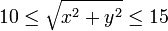
\includegraphics[scale=.6]{graphics/d8c852f6bb73b0d042422df261390347.png}.
Then display/plot them. The outcome should be a ``fuzzy'' circle. The
actual number of points plotted may be less than 100, given that some
pairs may be generated more than once.

There are several possible approaches to accomplish this. Here are two
possible algorithms.

1) Generate random pairs of integers and filter out those that don't
satisfy this condition:

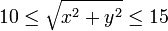
\includegraphics[scale=.6]{graphics/d8c852f6bb73b0d042422df261390347.png}.

2) Precalculate the set of all possible points (there are 404 of them)
and select randomly from this set.


\begin{wideverbatim}

(let Area (make (do 31 (link (need 31 " "))))
   (use (X Y)
      (do 100
         (until
            (>=
               15
               (sqrt
                  (+
                     (* (setq X (rand -15 15)) X)
                     (* (setq Y (rand -15 15)) Y) ) )
               10 ) )
         (set (nth Area (+ 16 X) (+ 16 Y)) "#") ) )
   (mapc prinl Area) )

Output:

           #
        ##
           #  #  #  #
         ## #    #  #   #
       #      #   # # #
    #       #     # #   #
      #   #         #    #
      #                #   #
                       #
       #               #
     ##                      #
                          #
   #                      # #
  ###                      #
 #                         # #
##                          # #
  #                        #
 #                        #
 ## #
                           #
   #
     #                 #
     #
   ###                  #   #
      ###           # #    #
    #      #
         #  #   ##
                 # #
      #     #           #
                # #  #

\end{wideverbatim}

\pagebreak{}
\section*{Constrained genericity}

\emph{Constrained genericity} means that a parametrized type or
function (see \emph{Parametric Polymorphism}) can only be instantiated
on types fulfilling some conditions, even if those conditions are not
used in that function.

Say a type is called ``eatable'' if you can call the function
\texttt{eat} on it. Write a generic type \texttt{FoodBox} which contains
a collection of objects of a type given as parameter, but can only be
instantiated on eatable types. The FoodBox shall not use the function
eat in any way (i.e. without the explicit restriction, it could be
instantiated on any type). The specification of a type being eatable
should be as generic as possible in your language (i.e. the restrictions
on the implementation of eatable types should be as minimal as
possible). Also explain the restrictions, if any, on the implementation
of eatable types, and show at least one example of an eatable type.



\begin{wideverbatim}

(class +Eatable)

(dm eat> ()
   (prinl "I'm eatable") )


(class +FoodBox)
# obj

(dm set> (Obj)
   (unless (method 'eat> Obj)                # Check if the object is eatable
      (quit "Object is not eatable" Obj) )
   (=: obj Obj) )                            # If so, set the object


(let (Box (new '(+FoodBox))  Eat (new '(+Eatable))  NoEat (new '(+Bla)))
   (set> Box Eat)       # Works
   (set> Box NoEat) )   # Gives an error

Output:

\$384320489 -- Object is not eatable

? (show Box)
\$384320487 (+FoodBox)
   obj \$384320488

? (show Box 'obj)
\$384320488 (+Eatable)

? (show NoEat)
\$384320489 (+Bla)

\end{wideverbatim}

\pagebreak{}
\section*{Conway's Game of Life}

The \textbf{Game of Life} is a
\href{http://en.wikipedia.org/wiki/cellular\_automaton}{cellular
  automaton} devised by the British mathematician
\href{http://en.wikipedia.org/wiki/John\_Horton\_Conway}{John Horton
  Conway} in 1970. It is the best-known example of a cellular
automaton.

Conway's game of life is described
\href{http://en.wikipedia.org/wiki/Conway\%27s\_Game\_of\_Life}{here}:

A cell \textbf{C} is represented by a 1 when alive or 0 when dead, in an
m-by-m square array of cells. We calculate \textbf{N} - the sum of live
cells in C's
\href{http://en.wikipedia.org/wiki/Moore\_neighborhood}{eight-location
neighbourhood}, then cell C is alive or dead in the next generation
based on the following table:

\begin{wideverbatim}
   C   N                 new C
   1   0,1             ->  0  # Lonely
   1   4,5,6,7,8       ->  0  # Overcrowded
   1   2,3             ->  1  # Lives
   0   3               ->  1  # It takes three to give birth!
   0   0,1,2,4,5,6,7,8 ->  0  # Barren
\end{wideverbatim}

Assume cells beyond the boundary are always dead.

The ``game'' is actually a zero-player game, meaning that its evolution
is determined by its initial state, needing no input from human players.
One interacts with the Game of Life by creating an initial configuration
and observing how it evolves.

Although you should test your implementation on more complex examples
such as the
\href{http://en.wikipedia.org/wiki/Conway\%27s\_Game\_of\_Life\#Examples\_of\_patterns}{glider}
in a larger universe, show the action of the blinker (three adjoining
cells in a row all alive), over three generations, in a 3 by 3 grid.



\begin{wideverbatim}

This example uses 'grid' and 'disp' from "lib/simul.l". These functions
maintain an array of multiply linked objects, and are also used in the chess
program and other games in the distribution.

(load "@lib/simul.l")
 
(de life (DX DY . Init)
   (let Grid (grid DX DY)
      (for This Init
         (=: life T) )
      (loop
         (disp Grid NIL
            '((This) (if (: life) "X " "  ")) )
         (wait 1000)
         (for Col Grid
            (for This Col
               (let N  # Count neighbors
                  (cnt
                     '((Dir) (get (Dir This) 'life))
                     (quote
                        west east south north
                        ((X) (south (west X)))
                        ((X) (north (west X)))
                        ((X) (south (east X)))
                        ((X) (north (east X))) ) )
                  (=: next  # Next generation
                     (if (: life)
                        (>= 3 N 2)
                        (= N 3) ) ) ) ) )
         (for Col Grid  # Update
            (for This Col
               (=: life (: next)) ) ) ) ) )
 
(life 5 5  b3 c3 d3)

\end{wideverbatim}

\begin{wideverbatim}
Output:

 5
 4
 3   X X X
 2
 1
   a b c d e
 5
 4     X
 3     X
 2     X
 1
   a b c d e
 5
 4
 3   X X X
 2
 1
   a b c d e

\end{wideverbatim}

\pagebreak{}
\section*{Copy a string}

This task is about copying a string. Where it is relevant, distinguish
between copying the contents of a string versus making an additional
reference to an existing string.

\begin{wideverbatim}

(setq Str1 "abcdef")
(setq Str2 Str1)                       # Create a reference to that symbol
(setq Str3 (name Str1))                # Create new symbol with name "abcdef"

\end{wideverbatim}

\pagebreak{}
\section*{Count occurrences of a substring}

The task is to either create a function, or show a built-in function, to
count the number of non-overlapping occurrences of a substring inside a
string. The function should take two arguments: the first argument being
the string to search and the second a substring to be search for. It
should return an integer count.

\begin{wideverbatim}

print countSubstring("the three truths","th")
3

// do not count substrings that overlap with
// previously-counted substrings:

print countSubstring("ababababab","abab")
2

\end{wideverbatim}

The matching should yield the highest number of non-overlapping matches.
In general, this essentially means matching from left-to-right or
right-to-left.


\begin{wideverbatim}

(de countSubstring (Str Sub)
   (let (Cnt 0  H (chop Sub))
      (for (S (chop Str)  S  (cdr S))
         (when (head H S)
            (inc 'Cnt)
            (setq S (map prog2 H S)) ) )
      Cnt ) )

Test:

: (countSubstring "the three truths" "th")
-> 3

: (countSubstring "ababababab" "abab")
-> 2

\end{wideverbatim}

\pagebreak{}
\section*{Count the Coins}


There are four types of common coins in US currency: quarters (25
cents), dimes (10), nickels (5) and pennies (1). There are 6 ways to
make change for 15 cents:

\begin{itemize}
\item
  A dime and a nickel;
\item
  A dime and 5 pennies;
\item
  3 nickels;
\item
  2 nickels and 5 pennies;
\item
  A nickel and 10 pennies;
\item
  15 pennies.
\end{itemize}

How many ways are there to make change for a dollar using these common
coins? (1 dollar = 100 cents).

\textbf{Optional:}

Less common are dollar coins (100 cents); very rare are half dollars (50
cents). With the addition of these two coins, how many ways are there to
make change for \$1000? (note: the answer is larger than
2\textsuperscript{32}).

\textbf{Algorithm}: See

\href{http://mitpress.mit.edu/sicp/full-text/book/book-Z-H-11.html\#\%\_sec\_Temp\_52}{http://mitpress.mit.edu/sicp/full-text/book/book-Z-H-11.html\#\%\_sec\_Temp\_52}.


\begin{wideverbatim}

(de coins (Sum Coins)
   (let (Buf (mapcar '((N) (cons 1 (need (dec N) 0))) Coins)  Prev)
      (do Sum
         (zero Prev)
         (for L Buf
            (inc (rot L) Prev)
            (setq Prev (car L)) ) )
      Prev ) )

Test:

(for Coins '((100 50 25 10 5 1) (200 100 50 20 10 5 2 1))
   (println (coins 100 (cddr Coins)))
   (println (coins (* 1000 100) Coins))
   (println (coins (* 10000 100) Coins))
   (println (coins (* 100000 100) Coins))
   (prinl) )

Output:

242
13398445413854501
1333983445341383545001
133339833445334138335450001

4562
10056050940818192726001
99341140660285639188927260001
992198221207406412424859964272600001

\end{wideverbatim}

\pagebreak{}
\section*{Counting in Factors}

Write a program which counts up from 1, displaying each number as the
multiplication of its prime factors. For the purpose of this task, 1 may
be shown as itself.

For examle, 2 is prime, so it would be shown as itself. 6 is not prime;
it would be shown as

\includegraphics[scale=.6]{graphics/4b3a89ff7af9ad06700897f831201197.png}.

Likewise, 2144 is not prime; it would be shown as

\includegraphics[scale=.6]{graphics/eae4d1b7a3788fd85e5c4995efc7e196.png}.

c.f. \emph{Prime decomposition}, \emph{Category:Prime\_Numbers}


\begin{wideverbatim}

This is the 'factor' function from [[Prime decomposition#PicoLisp]].

(de factor (N)
   (make
      (let (D 2  L (1 2 2 . (4 2 4 2 4 6 2 6 .))  M (sqrt N))
         (while (>= M D)
            (if (=0 (\% N D))
               (setq M (sqrt (setq N (/ N (link D)))))
               (inc 'D (pop 'L)) ) )
         (link N) ) ) )

(for N 20
   (prinl N ": " (glue " * " (factor N))) )

Output:

1: 1
2: 2
3: 3
4: 2 * 2
5: 5
6: 2 * 3
7: 7
8: 2 * 2 * 2
9: 3 * 3
10: 2 * 5
11: 11
12: 2 * 2 * 3
13: 13
14: 2 * 7
15: 3 * 5
16: 2 * 2 * 2 * 2
17: 17
18: 2 * 3 * 3
19: 19
20: 2 * 2 * 5

\end{wideverbatim}

\pagebreak{}
\section*{Counting in octal}

The task is to produce a sequential count in octal, starting at zero,
and using an increment of a one for each consecutive number. Each number
should appear on a single line, and the program should count until
terminated, or until the maximum value of the numeric type in use is
reached.

\begin{itemize}
\item \emph{Integer sequence} is a similar task without the use of
  octal numbers.
\end{itemize}


\begin{wideverbatim}

(for (N 0  T  (inc N))
   (prinl (oct N)) )

\end{wideverbatim}

\pagebreak{}
\section*{Create a file}

In this task, the job is to create a new empty file called
``output.txt'' of size 0 bytes and an empty directory called ``docs''.
This should be done twice: once ``here'', i.e. in the current working
directory and once in the filesystem root.


\begin{wideverbatim}

(out "output.txt")                     # Empty output
(call 'mkdir "docs")                   # Call external
(out "/output.txt")
(call 'mkdir "/docs")

\end{wideverbatim}

\pagebreak{}
\section*{Create a two-dimensional array at runtime}


\textbf{Data Structure}\\ This illustrates a data structure, a means of
storing data within a program.

You may see other such structures in the \emph{Data Structures}
category.

Get two integers from the user, then create a two-dimensional array
where the two dimensions have the sizes given by those numbers, and
which can be accessed in the most natural way possible. Write some
element of that array, and then output that element. Finally destroy
the array if not done by the language itself.


\begin{wideverbatim}

(de 2dimTest (DX DY)
   (let A (make (do DX (link (need DY))))
      (set (nth A 3 3) 999)            # Set A[3][3] to 999
      (mapc println A)                 # Print all
      (get A 3 3) ) )                  # Return A[3][3]

(2dimTest 5 5)

Output:

(NIL NIL NIL NIL NIL)
(NIL NIL NIL NIL NIL)
(NIL NIL 999 NIL NIL)
(NIL NIL NIL NIL NIL)
(NIL NIL NIL NIL NIL)
-> 999

\end{wideverbatim}

\pagebreak{}
\section*{Create an HTML table}


Create an HTML table.

\begin{itemize}
\item
  The table body should have at least three rows of three columns.
\item
  Each of these three columns should be labelled ``X'', ``Y'', and
  ``Z''.
\item
  An extra column should be added at either the extreme left or the
  extreme right of the table that has no heading, but is filled with
  sequential row numbers.
\item
  The rows of the ``X'', ``Y'', and ``Z'' columns should be filled with
  random or sequential integers having 4 digits or less.
\item
  The numbers should be aligned in the same fashion for all columns.
\end{itemize}



\begin{wideverbatim}

(load "@lib/xhtml.l")

(<table> NIL NIL '(NIL (NIL "X") (NIL "Y") (NIL "Z"))
   (for N 3
      (<row> NIL N 124 456 789) ) )

\end{wideverbatim}

\pagebreak{}
\section*{Create an object at a given address}


\textbf{Basic Data Operation}\\ This is a basic data operation. It
represents a fundamental action on a basic data type.

You may see other such operations in the \emph{Basic Data Operations}
category, or:

\textbf{Integer Operations} \\
\emph{Arithmetic} \textbar{} \emph{Comparison}

\textbf{Boolean Operations} \\ \emph{Bitwise} \textbar{}
\emph{Logical}

\textbf{String Operations} \\
\emph{Concatenation} \textbar{} \emph{Interpolation} \textbar{}
\emph{Matching}

\textbf{Memory Operations} \\
\emph{Pointers \& references} \textbar{} \emph{Addresses}

In systems programing it is sometimes required to place language objects
at specific memory locations, like I/O registers, hardware interrupt
vectors etc.

\textbf{Task}

Show how language objects can be allocated at a specific machine
addresses.

Since most \emph{OSes} prohibit access to the physical memory if it is
not mapped by the application, as an example, rather than a physical
address, take the address of some existing object (using suitable
\emph{address operations} if necessary). For example, create an
integer object. Print the machine address of the object. Take the
address of the object and create another integer object at this
address. Print the value of this object to verify that it is same as
one of the origin. Change the value of the origin and verify it again.


\begin{wideverbatim}

: (setq IntSpace 12345)          # Integer
-> 12345

: (setq Address (adr 'IntSpace)) # Encoded machine address
-> -2969166782547

: (set (adr Address) 65535)      # Set this address to a new value
-> 65535

: IntSpace                       # Show the new value
-> 65535

\end{wideverbatim}

\pagebreak{}
\section*{CSV to HTML translation}


Consider a simplified CSV format where all rows are separated by a
newline and all columns are separated by commas. No commas are allowed
as field data, but the data may contain other characters and character
sequences that would normally be escaped when converted to HTML

The task is to create a function that takes a string representation of
the CSV data and returns a text string of an HTML table representing the
CSV data. Use the following data as the CSV text to convert, and show
your output.

Character,Speech

The multitude,The messiah! Show us the messiah!

Brians mother,\textless{}angry\textgreater{}Now you listen here! He's
not the messiah; he's a very naughty boy! Now go
away!\textless{}/angry\textgreater{}

The multitude,Who are you?

Brians mother,I'm his mother; that's who!

The multitude,Behold his mother! Behold his mother!

For extra credit, \emph{optionally} allow special formatting for the
first row of the table as if it is the tables header row (via
\textless{}thead\textgreater{} preferably; CSS if you must).



\begin{wideverbatim}

Simple solution

(load "@lib/http.l")

(in "text.csv"
   (<table> 'myStyle NIL NIL
      (prinl)
      (while (split (line) ",")
         (<row> NIL (ht:Prin (pack (car @))) (ht:Prin (pack (cadr @))))
         (prinl) ) ) )

Output:

<table class="myStyle">
<tr><td>Character</td><td>Speech</td></tr>
<tr><td>The multitude</td><td>The messiah! Show us the messiah!</td></tr>
<tr><td>Brians mother</td><td>\&lt;angry\&gt;Now you listen here! 
He's not the messiah; he's a very naughty boy! Now go away!\&lt;/angry\&gt;</td></tr>
<tr><td>The multitude</td><td>Who are you?</td></tr>
<tr><td>Brians mother</td><td>I'm his mother; that's who!</td></tr>
<tr><td>The multitude</td><td>Behold his mother! Behold his mother!</td></tr>
</table>

Extra credit solution

(load "@lib/http.l")

(in "text.csv"
   (when (split (line) ",")
      (<table> 'myStyle NIL (mapcar '((S) (list NIL (pack S))) @)
         (prinl)
         (while (split (line) ",")
            (<row> NIL (ht:Prin (pack (car @))) (ht:Prin (pack (cadr @))))
            (prinl) ) ) ) )

Output:

<table class="myStyle"><tr><th>Character</th><th>Speech</th></tr>
<tr><td>The multitude</td><td>The messiah! Show us the messiah!</td></tr>
<tr><td>Brians mother</td><td>\&lt;angry\&gt;Now you listen here! 
He's not the messiah; he's a very naughty boy! Now go away!\&lt;/angry\&gt;</td></tr>
<tr><td>The multitude</td><td>Who are you?</td></tr>
<tr><td>Brians mother</td><td>I'm his mother; that's who!</td></tr>
<tr><td>The multitude</td><td>Behold his mother! Behold his mother!</td></tr>
</table>

\end{wideverbatim}


% %%%%%%%%%%%%%%%%%%%%%%%% referenc.tex %%%%%%%%%%%%%%%%%%%%%%%%%%%%%%
% sample references
% %
% Use this file as a template for your own input.
%
%%%%%%%%%%%%%%%%%%%%%%%% Springer-Verlag %%%%%%%%%%%%%%%%%%%%%%%%%%
%
% BibTeX users please use
% \bibliographystyle{}
% \bibliography{}
%
\biblstarthook{In view of the parallel print and (chapter-wise) online publication of your book at \url{www.springerlink.com} it has been decided that -- as a genreral rule --  references should be sorted chapter-wise and placed at the end of the individual chapters. However, upon agreement with your contact at Springer you may list your references in a single seperate chapter at the end of your book. Deactivate the class option \texttt{sectrefs} and the \texttt{thebibliography} environment will be put out as a chapter of its own.\\\indent
References may be \textit{cited} in the text either by number (preferred) or by author/year.\footnote{Make sure that all references from the list are cited in the text. Those not cited should be moved to a separate \textit{Further Reading} section or chapter.} The reference list should ideally be \textit{sorted} in alphabetical order -- even if reference numbers are used for the their citation in the text. If there are several works by the same author, the following order should be used: 
\begin{enumerate}
\item all works by the author alone, ordered chronologically by year of publication
\item all works by the author with a coauthor, ordered alphabetically by coauthor
\item all works by the author with several coauthors, ordered chronologically by year of publication.
\end{enumerate}
The \textit{styling} of references\footnote{Always use the standard abbreviation of a journal's name according to the ISSN \textit{List of Title Word Abbreviations}, see \url{http://www.issn.org/en/node/344}} depends on the subject of your book:
\begin{itemize}
\item The \textit{two} recommended styles for references in books on \textit{mathematical, physical, statistical and computer sciences} are depicted in ~\cite{science-contrib, science-online, science-mono, science-journal, science-DOI} and ~\cite{phys-online, phys-mono, phys-journal, phys-DOI, phys-contrib}.
\item Examples of the most commonly used reference style in books on \textit{Psychology, Social Sciences} are~\cite{psysoc-mono, psysoc-online,psysoc-journal, psysoc-contrib, psysoc-DOI}.
\item Examples for references in books on \textit{Humanities, Linguistics, Philosophy} are~\cite{humlinphil-journal, humlinphil-contrib, humlinphil-mono, humlinphil-online, humlinphil-DOI}.
\item Examples of the basic Springer style used in publications on a wide range of subjects such as \textit{Computer Science, Economics, Engineering, Geosciences, Life Sciences, Medicine, Biomedicine} are ~\cite{basic-contrib, basic-online, basic-journal, basic-DOI, basic-mono}. 
\end{itemize}
}

\begin{thebibliography}{99.}%
% and use \bibitem to create references.
%
% Use the following syntax and markup for your references if 
% the subject of your book is from the field 
% "Mathematics, Physics, Statistics, Computer Science"
%
% Contribution 
\bibitem{science-contrib} Broy, M.: Software engineering --- from auxiliary to key technologies. In: Broy, M., Dener, E. (eds.) Software Pioneers, pp. 10-13. Springer, Heidelberg (2002)
%
% Online Document
\bibitem{science-online} Dod, J.: Effective substances. In: The Dictionary of Substances and Their Effects. Royal Society of Chemistry (1999) Available via DIALOG. \\
\url{http://www.rsc.org/dose/title of subordinate document. Cited 15 Jan 1999}
%
% Monograph
\bibitem{science-mono} Geddes, K.O., Czapor, S.R., Labahn, G.: Algorithms for Computer Algebra. Kluwer, Boston (1992) 
%
% Journal article
\bibitem{science-journal} Hamburger, C.: Quasimonotonicity, regularity and duality for nonlinear systems of partial differential equations. Ann. Mat. Pura. Appl. \textbf{169}, 321--354 (1995)
%
% Journal article by DOI
\bibitem{science-DOI} Slifka, M.K., Whitton, J.L.: Clinical implications of dysregulated cytokine production. J. Mol. Med. (2000) doi: 10.1007/s001090000086 
%
\bigskip

% Use the following (APS) syntax and markup for your references if 
% the subject of your book is from the field 
% "Mathematics, Physics, Statistics, Computer Science"
%
% Online Document
\bibitem{phys-online} J. Dod, in \textit{The Dictionary of Substances and Their Effects}, Royal Society of Chemistry. (Available via DIALOG, 1999), 
\url{http://www.rsc.org/dose/title of subordinate document. Cited 15 Jan 1999}
%
% Monograph
\bibitem{phys-mono} H. Ibach, H. L\"uth, \textit{Solid-State Physics}, 2nd edn. (Springer, New York, 1996), pp. 45-56 
%
% Journal article
\bibitem{phys-journal} S. Preuss, A. Demchuk Jr., M. Stuke, Appl. Phys. A \textbf{61}
%
% Journal article by DOI
\bibitem{phys-DOI} M.K. Slifka, J.L. Whitton, J. Mol. Med., doi: 10.1007/s001090000086
%
% Contribution 
\bibitem{phys-contrib} S.E. Smith, in \textit{Neuromuscular Junction}, ed. by E. Zaimis. Handbook of Experimental Pharmacology, vol 42 (Springer, Heidelberg, 1976), p. 593
%
\bigskip
%
% Use the following syntax and markup for your references if 
% the subject of your book is from the field 
% "Psychology, Social Sciences"
%
%
% Monograph
\bibitem{psysoc-mono} Calfee, R.~C., \& Valencia, R.~R. (1991). \textit{APA guide to preparing manuscripts for journal publication.} Washington, DC: American Psychological Association.
%
% Online Document
\bibitem{psysoc-online} Dod, J. (1999). Effective substances. In: The dictionary of substances and their effects. Royal Society of Chemistry. Available via DIALOG. \\
\url{http://www.rsc.org/dose/Effective substances.} Cited 15 Jan 1999.
%
% Journal article
\bibitem{psysoc-journal} Harris, M., Karper, E., Stacks, G., Hoffman, D., DeNiro, R., Cruz, P., et al. (2001). Writing labs and the Hollywood connection. \textit{J Film} Writing, 44(3), 213--245.
%
% Contribution 
\bibitem{psysoc-contrib} O'Neil, J.~M., \& Egan, J. (1992). Men's and women's gender role journeys: Metaphor for healing, transition, and transformation. In B.~R. Wainrig (Ed.), \textit{Gender issues across the life cycle} (pp. 107--123). New York: Springer.
%
% Journal article by DOI
\bibitem{psysoc-DOI}Kreger, M., Brindis, C.D., Manuel, D.M., Sassoubre, L. (2007). Lessons learned in systems change initiatives: benchmarks and indicators. \textit{American Journal of Community Psychology}, doi: 10.1007/s10464-007-9108-14.
%
%
% Use the following syntax and markup for your references if 
% the subject of your book is from the field 
% "Humanities, Linguistics, Philosophy"
%
\bigskip
%
% Journal article
\bibitem{humlinphil-journal} Alber John, Daniel C. O'Connell, and Sabine Kowal. 2002. Personal perspective in TV interviews. \textit{Pragmatics} 12:257--271
%
% Contribution 
\bibitem{humlinphil-contrib} Cameron, Deborah. 1997. Theoretical debates in feminist linguistics: Questions of sex and gender. In \textit{Gender and discourse}, ed. Ruth Wodak, 99--119. London: Sage Publications.
%
% Monograph
\bibitem{humlinphil-mono} Cameron, Deborah. 1985. \textit{Feminism and linguistic theory.} New York: St. Martin's Press.
%
% Online Document
\bibitem{humlinphil-online} Dod, Jake. 1999. Effective substances. In: The dictionary of substances and their effects. Royal Society of Chemistry. Available via DIALOG. \\
http://www.rsc.org/dose/title of subordinate document. Cited 15 Jan 1999
%
% Journal article by DOI
\bibitem{humlinphil-DOI} Suleiman, Camelia, Daniel C. O�Connell, and Sabine Kowal. 2002. `If you and I, if we, in this later day, lose that sacred fire...�': Perspective in political interviews. \textit{Journal of Psycholinguistic Research}. doi: 10.1023/A:1015592129296.
%
%
%
\bigskip
%
%
% Use the following syntax and markup for your references if 
% the subject of your book is from the field 
% "Computer Science, Economics, Engineering, Geosciences, Life Sciences"
%
%
% Contribution 
\bibitem{basic-contrib} Brown B, Aaron M (2001) The politics of nature. In: Smith J (ed) The rise of modern genomics, 3rd edn. Wiley, New York 
%
% Online Document
\bibitem{basic-online} Dod J (1999) Effective Substances. In: The dictionary of substances and their effects. Royal Society of Chemistry. Available via DIALOG. \\
\url{http://www.rsc.org/dose/title of subordinate document. Cited 15 Jan 1999}
%
% Journal article by DOI
\bibitem{basic-DOI} Slifka MK, Whitton JL (2000) Clinical implications of dysregulated cytokine production. J Mol Med, doi: 10.1007/s001090000086
%
% Journal article
\bibitem{basic-journal} Smith J, Jones M Jr, Houghton L et al (1999) Future of health insurance. N Engl J Med 965:325--329
%
% Monograph
\bibitem{basic-mono} South J, Blass B (2001) The future of modern genomics. Blackwell, London 
%
\end{thebibliography}


%%%%%%%%%%%%%%%%%%%%% chapter.tex %%%%%%%%%%%%%%%%%%%%%%%%%%%%%%%%%
%
% sample chapter
%
% Use this file as a template for your own input.
%
%%%%%%%%%%%%%%%%%%%%%%%% Springer-Verlag %%%%%%%%%%%%%%%%%%%%%%%%%%
%\motto{Use the template \emph{chapter.tex} to style the various elements of your chapter content.}

\chapter{Rosetta Code Tasks starting with D}

\section*{Date format}


This task has been clarified. Its programming examples are in need of
review to ensure that they still fit the requirements of the task.

Display the current date in the formats of ``2007-11-10'' and ``Sunday,
November 10, 2007''.

\begin{wideverbatim}

(let (Date (date)  Lst (date Date))
   (prinl (dat\$ Date "-"))             # 2010-02-19
   (prinl                              # Friday, February 19, 2010
      (day Date)
      ", "
      (get *MonFmt (cadr Lst))
      " "
      (caddr Lst)
      ", "
      (car Lst) ) )

\end{wideverbatim}

\pagebreak{}
\section*{Date manipulation}

Given the date string ``March 7 2009 7:30pm EST'', output the time 12
hours later in any human-readable format.

As extra credit, display the resulting time in a time zone different
from your own.

\begin{wideverbatim}

(de timePlus12 (Str)
   (use (@Mon @Day @Year @Time @Zone)
      (and
         (match
            '(@Mon " " @Day " " @Year " " @Time " " @Zone)
            (chop Str) )
         (setq @Mon (index (pack @Mon) *MonFmt))
         (setq @Day (format @Day))
         (setq @Year (format @Year))
         (setq @Time
            (case (tail 2 @Time)
               (("a" "m") (\$tim (head -2 @Time)))
               (("p" "m") (+ `(time 12 0) (\$tim (head -2 @Time))))
               (T (\$tim @Time)) ) )
         (let? Date (date @Year @Mon @Day)
            (when (>= (inc '@Time `(time 12 0)) 86400)
               (dec '@Time 86400)
               (inc 'Date) )
            (pack (dat\$ Date "-") " " (tim\$ @Time T) " " @Zone) ) ) ) )

\end{wideverbatim}

\pagebreak{}
\section*{Day of the week}

A company decides that whenever Xmas falls on a Sunday they will give
their workers all extra paid holidays so that, together with any public
holidays, workers will not have to work the following week (between the
25th of December and the first of January).

\textbf{In what years between 2008 and 2121 will the 25th of December be
a Sunday?}

Using any standard date handling libraries of your programming language;
compare the dates calculated with the output of other languages to
discover any anomalies in the handling of dates which may be due to, for
example, overflow in types used to represent dates/times similar to
\href{http://en.wikipedia.org/wiki/Y2k\#See\_also}{y2k} type problems.


\begin{wideverbatim}

(for (Y 2008 (>= 2121 Y) (inc Y))
   (when (= "Sunday" (day (date Y 12 25)))
      (printsp Y) ) )

Output:

2011 2016 2022 2033 2039 2044 2050 2061 2067 2072 2078 2089 2095 2101 2107 2112 2118

\end{wideverbatim}

\pagebreak{}
\section*{Deal cards for FreeCell}

\emph{Free Cell} is the solitaire card game that Paul Alfille
introduced to the PLATO system in 1978. Jim Horne, at Microsoft,
changed the name to \emph{FreeCell} and reimplemented the game for
\emph{DOS}, then \emph{Windows}. This version introduced 32000
numbered deals. (The
\href{http://www.solitairelaboratory.com/fcfaq.html}{FreeCell FAQ}
tells this history.)

As the game became popular, Jim Horne disclosed
\href{http://www.solitairelaboratory.com/mshuffle.txt}{the algorithm},
and other implementations of FreeCell began to reproduce the Microsoft
deals. These deals are numbered from 1 to 32000. Newer versions from
Microsoft have 1 million deals, numbered from 1 to 1000000; some
implementations allow numbers outside that range.

The algorithm uses this \emph{linear congruential generator} from
Microsoft C:

\begin{itemize}
\item
  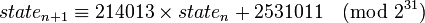
\includegraphics[scale=.6]{graphics/47c16228f3793455eb3436c78d21477d.png}
\item
  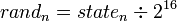
\includegraphics[scale=.6]{graphics/a026db06e1a9bd6945c85c8e17231725.png}
\item
  \emph{r}\emph{a}\emph{n}\emph{d}\textsubscript{\emph{n}} is in range 0
  to 32767.
\item Rosetta Code has another task, \emph{linear congruential
    generator}, with code for this RNG in several languages.
\end{itemize}

The algorithm follows:

\begin{enumerate}
\item
  Seed the RNG with the number of the deal.
\item
  Create an \emph{array} of 52 cards: Ace of Clubs, Ace of
  Diamonds, Ace of Hearts, Ace of Spades, 2 of Clubs, 2 of Diamonds, and
  so on through the ranks: Ace, 2, 3, 4, 5, 6, 7, 8, 9, 10, Jack, Queen,
  King. The array indexes are 0 to 51, with Ace of Clubs at 0, and King
  of Spades at 51.
\item
  Until the array is empty:

  \begin{itemize}
  \item
    Choose a random card at \emph{index} ≡ \emph{next random number}
    (mod \emph{array length}).
  \item
    Swap this random card with the last card of the array.
  \item
    Remove this random card from the array. (Array length goes down by
    1.)
  \item
    Deal this random card.
  \end{itemize}
\item
  Deal all 52 cards, face up, across 8 columns. The first 8 cards go in
  8 columns, the next 8 cards go on the first 8 cards, and so on.
\end{enumerate}

\pagebreak{}
\begin{verbatim}
Order to deal cards

 1  2  3  4  5  6  7  8
 9 10 11 12 13 14 15 16
17 18 19 20 21 22 23 24
25 26 27 28 29 30 31 32
33 34 35 36 37 38 39 40
41 42 43 44 45 46 47 48
49 50 51 52
\end{verbatim}

\begin{verbatim}
Game \#1

JD 2D 9H JC 5D 7H 7C 5H
KD KC 9S 5S AD QC KH 3H
2S KS 9D QD JS AS AH 3C
4C 5C TS QH 4H AC 4D 7S
3S TD 4S TH 8H 2C JH 7D
6D 8S 8D QS 6C 3D 8C TC
6S 9C 2H 6H
\end{verbatim}

\begin{verbatim}
Game \#617

7D AD 5C 3S 5S 8C 2D AH
TD 7S QD AC 6D 8H AS KH
TH QC 3H 9D 6S 8D 3D TC
KD 5H 9S 3C 8S 7H 4D JS
4C QS 9C 9H 7C 6H 2C 2S
4S TS 2H 5D JC 6C JH QH
JD KS KC 4H
\end{verbatim}

Deals can also be checked against
\href{http://freecellgamesolutions.com/}{FreeCell solutions to 1000000
  games}. (Summon a video solution, and it displays the initial deal.)

Write a program to take a deal number and deal cards in the same order
as this algorithm. The program may display the cards with ASCII, with
Unicode, by drawing graphics, or any other way.


\begin{wideverbatim}

Using the random generator from [[Linear congruential generator#PicoLisp]]:

(setq *MsSeed 11982)

(de msRand ()
   (>> 16
      (setq *MsSeed
         (\& (+ 2531011 (* 214013 *MsSeed)) `(dec (** 2 31))) ) ) )

(let L
   (make
      (for Num (range 13 1)
         (for Suit '((32 . "♠") (31 . "♥") (31 . "♦") (32 . "♣"))
            (link (cons (get '`(chop "A23456789TJQK") Num) Suit)) ) ) )
   (for I 51
      (xchg
         (nth L I)
         (nth L (- 52 (\% (msRand) (- 53 I)))) ) )
   (for C L
      (prin "  ^[[" (cadr C) "m" (cddr C) "^[[m" (car C))
      (at (0 . 8) (prinl)) )
   (prinl) )

\end{wideverbatim}

\pagebreak{}
\section*{Decision tables}

\href{http://en.wikipedia.org/wiki/Decision\_table}{Decision Tables} are
a precise yet compact way to model complicated logic. Demonstrate how
your language implements decision tables. Use the example of Printer
Troubleshooting given in the Wikipedia article.

\begin{wideverbatim}

We allow ourselves a luxurious user interface:

(de yes? (Cond)
   (out NIL (prin (car Cond) "? "))
   (in NIL
      (use Reply
         (loop
            (setq Reply (read))
            (T (member Reply '(T Y YES Yes y yes true 1))
               T )
            (T (member Reply '(NIL N NO No n no false 0)))
            (prinl "Please answer 'Yes' or 'No'") ) ) ) )

The decision table used in the example:

(de *Conditions
   ("Printer does not print"                T   T   T   T  NIL NIL NIL NIL)
   ("A red light is flashing"               T   T  NIL NIL  T   T  NIL NIL)
   ("Printer is unrecognised"               T  NIL  T  NIL  T  NIL  T  NIL) )

(de *Actions
   ("Check the power cable"                NIL NIL  T)
   ("Check the printer-computer cable"      T  NIL  T)
   ("Ensure printer software is installed"  T  NIL  T  NIL  T  NIL  T)
   ("Check/replace ink"                     T   T  NIL NIL  T   T)
   ("Check for paper jam"                  NIL  T  NIL  T) )

The decision can be made directly on the condition and action data, without the
need to create intermediate tables:

(de decide ()
   (let Reply (mapcar yes? *Conditions)
      (extract and
         (apply pick (append *Conditions *Actions)
            '(@
               (unless (pick '((Flg) (<> Flg (next))) Reply)
                  (rest) ) ) )
         (mapcar car *Actions) ) ) )


\end{wideverbatim}

\begin{wideverbatim}

Output:

: (decide)
Printer does not print? y
A red light is flashing? y
Printer is unrecognised? n
-> ("Check/replace ink" "Check for paper jam")

: (decide)
Printer does not print? n
A red light is flashing? y
Printer is unrecognised? y
-> ("Ensure printer software is installed" "Check/replace ink")

: (decide)
Printer does not print? n
A red light is flashing? n
Printer is unrecognised? n
-> NIL

\end{wideverbatim}


\pagebreak{}
\section*{Deconvolution/1D}

The convolution of two functions \emph{F} and \emph{H} of an integer
variable is defined as the function \emph{G} satisfying

\begin{figure}[H]
\centering
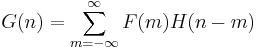
\includegraphics[scale=.6]{graphics/e4e4d6b17e1e15dbddc307340f0a620f.png}
% \caption{ G(n) =
% \textbackslash{}sum\_\{m=-\textbackslash{}infty\}\^{}\{\textbackslash{}infty\}
% F(m) H(n-m) }
\end{figure}

for all integers \emph{n}. Assume \emph{F}(\emph{n}) can be non-zero
only for 0 ≤ \emph{n} ≤ \textbar{} \emph{F} \textbar{} , where
\textbar{} \emph{F} \textbar{} is the ``length'' of \emph{F}, and
similarly for \emph{G} and \emph{H}, so that the functions can be
modeled as finite sequences by identifying
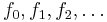
\includegraphics[scale=.6]{graphics/b14d36d888dae449d5c4fcfb6f4ff8ce.png}
with

\includegraphics[scale=.6]{graphics/2eb0e52a9d4ca2a57f0a0ceaca866399.png},
etc. Then for example, values of \textbar{} \emph{F} \textbar{} = 6 and
\textbar{} \emph{H} \textbar{} = 5 would determine the following value
of \emph{g} by definition.

\begin{figure}[H]
\centering
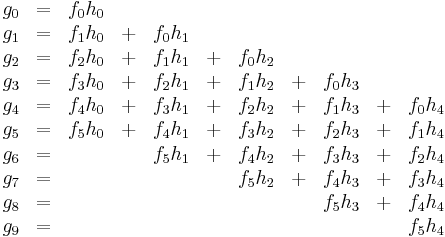
\includegraphics[scale=.6]{graphics/7f867e9ec901e62d2c8efa1ec9b4c5d6.png}
% \caption{ \textbackslash{}begin\{array\}\{lllllllllll\} g\_0 \&=
% \&f\_0h\_0\textbackslash{}\textbackslash{} g\_1 \&= \&f\_1h\_0 \&+
% \&f\_0h\_1\textbackslash{}\textbackslash{} g\_2 \&= \&f\_2h\_0 \&+
% \&f\_1h\_1 \&+ \&f\_0h\_2\textbackslash{}\textbackslash{} g\_3 \&=
% \&f\_3h\_0 \&+ \&f\_2h\_1 \&+ \&f\_1h\_2 \&+
% \&f\_0h\_3\textbackslash{}\textbackslash{} g\_4 \&= \&f\_4h\_0 \&+
% \&f\_3h\_1 \&+ \&f\_2h\_2 \&+ \&f\_1h\_3 \&+
% \&f\_0h\_4\textbackslash{}\textbackslash{} g\_5 \&= \&f\_5h\_0 \&+
% \&f\_4h\_1 \&+ \&f\_3h\_2 \&+ \&f\_2h\_3 \&+
% \&f\_1h\_4\textbackslash{}\textbackslash{} g\_6 \&= \& \& \&f\_5h\_1 \&+
% \&f\_4h\_2 \&+ \&f\_3h\_3 \&+ \&f\_2h\_4\textbackslash{}\textbackslash{}
% g\_7 \&= \& \& \& \& \&f\_5h\_2 \&+ \&f\_4h\_3 \&+
% \&f\_3h\_4\textbackslash{}\textbackslash{} g\_8 \&= \& \& \& \& \& \&
% \&f\_5h\_3 \&+ \&f\_4h\_4\textbackslash{}\textbackslash{} g\_9 \&= \& \&
% \& \& \& \& \& \& \&f\_5h\_4 \textbackslash{}end\{array\} }
\end{figure}

We can write this in matrix form as:

\begin{figure}[H]
\centering
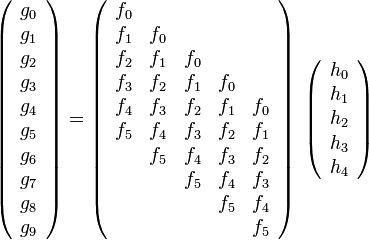
\includegraphics[scale=.6]{graphics/5cec990b9d6c1fdc3b340a364729aea6.png}
% \caption{ \textbackslash{}left( \textbackslash{}begin\{array\}\{l\} g\_0
% \textbackslash{}\textbackslash{} g\_1 \textbackslash{}\textbackslash{}
% g\_2 \textbackslash{}\textbackslash{} g\_3
% \textbackslash{}\textbackslash{} g\_4 \textbackslash{}\textbackslash{}
% g\_5 \textbackslash{}\textbackslash{} g\_6
% \textbackslash{}\textbackslash{} g\_7 \textbackslash{}\textbackslash{}
% g\_8 \textbackslash{}\textbackslash{} g\_9
% \textbackslash{}\textbackslash{} \textbackslash{}end\{array\}
% \textbackslash{}right) = \textbackslash{}left(
% \textbackslash{}begin\{array\}\{lllll\}
% f\_0\textbackslash{}\textbackslash{} f\_1 \&
% f\_0\textbackslash{}\textbackslash{} f\_2 \& f\_1 \&
% f\_0\textbackslash{}\textbackslash{} f\_3 \& f\_2 \& f\_1 \&
% f\_0\textbackslash{}\textbackslash{} f\_4 \& f\_3 \& f\_2 \& f\_1 \&
% f\_0\textbackslash{}\textbackslash{} f\_5 \& f\_4 \& f\_3 \& f\_2 \&
% f\_1\textbackslash{}\textbackslash{} \& f\_5 \& f\_4 \& f\_3 \&
% f\_2\textbackslash{}\textbackslash{} \& \& f\_5 \& f\_4 \&
% f\_3\textbackslash{}\textbackslash{} \& \& \& f\_5 \&
% f\_4\textbackslash{}\textbackslash{} \& \& \& \& f\_5
% \textbackslash{}end\{array\} \textbackslash{}right) \textbackslash{};
% \textbackslash{}left( \textbackslash{}begin\{array\}\{l\} h\_0
% \textbackslash{}\textbackslash{} h\_1 \textbackslash{}\textbackslash{}
% h\_2 \textbackslash{}\textbackslash{} h\_3
% \textbackslash{}\textbackslash{} h\_4 \textbackslash{}\textbackslash{}
% \textbackslash{}end\{array\} \textbackslash{}right) }
\end{figure}

or

\begin{figure}[H]
\centering
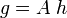
\includegraphics[scale=.6]{graphics/9321b2aa2a198225b0dbe56040b49940.png}
% \caption{ g = A \textbackslash{}; h }
\end{figure}

For this task, implement a function (or method, procedure, subroutine,
etc.) \texttt{deconv} to perform \emph{deconvolution} (i.e., the
\emph{inverse} of convolution) by constructing and solving such a system
of equations represented by the above matrix \emph{A} for \emph{h} given
\emph{f} and \emph{g}.

\begin{itemize}
\item
  The function should work for \emph{G} of arbitrary length (i.e., not
  hard coded or constant) and \emph{F} of any length up to that of
  \emph{G}. Note that \textbar{} \emph{H} \textbar{} will be given by
  \textbar{} \emph{G} \textbar{} − \textbar{} \emph{F} \textbar{} + 1.
\item There may be more equations than unknowns. If convenient, use a
  function from a
  \href{http://www.netlib.org/lapack/lug/node27.html}{library} that
  finds the best fitting solution to an overdetermined system of
  linear equations (as in the \emph{Multiple regression} task).
  Otherwise, prune the set of equations as needed and solve as in the
  \emph{Reduced row echelon form} task.
\item
  Test your solution on the following data. Be sure to verify both that
  \texttt{deconv}(\emph{g},\emph{f}) = \emph{h} and
  \texttt{deconv}(\emph{g},\emph{h}) = \emph{f} and display the results
  in a human readable form.
\end{itemize}

\begin{wideverbatim}

h = [-8,-9,-3,-1,-6,7] 

f = [-3,-6,-1,8,-6,3,-1,-9,-9,3,-2,5,2,-2,-7,-1]

g = [ 24,75,71,-34,3,22,-45,23,245,25,52,25,-67,-96,96,31,55,36,29,-43,-7]

\end{wideverbatim}

\begin{wideverbatim}

(load "@lib/math.l")
 
(de deconv (G F)
   (let A (pop 'F)
      (make
         (for (N . H) (head (- (length F)) G)
            (for (I . M) (made)
               (dec 'H
                  (*/ M (get F (- N I)) 1.0) ) )
            (link (*/ H 1.0 A)) ) ) ) )

Test:

(setq
   F (-3. -6. -1. 8. -6. 3. -1. -9. -9. 3. -2. 5. 2. -2. -7. -1.)
   G (24. 75. 71. -34. 3. 22. -45. 23. 245. 25. 52. 25. -67. -96.
   96. 31. 55. 36. 29. -43. -7.)
   H (-8. -9. -3. -1. -6. 7.) )
 
(test H (deconv G F))
(test F (deconv G H))

\end{wideverbatim}


\pagebreak{}
\section*{Deepcopy}

Demonstrate how to copy data structures containing complex
hetrogeneous and cyclic semantics. This is often referred to as
\href{http://en.wikipedia.org/wiki/Deep\_copy\#Deep\_copy}{deep
  copying}, and is normally required where structures are mutable and
to ensure that independent copies can be manipulated without
side-effects.

If this facility is not built into the language, it is permissible to
use functions from a common library, or a coded procedure.

The task should show:

\begin{itemize}
\item
  Relevant semantics of structures, such as their
  \href{http://en.wikipedia.org/wiki/Homogeneity\_and\_heterogeneity}{homogeneous
  or heterogeneous} properties, or containment of (self- or
  mutual-reference) cycles.
\end{itemize}

\begin{itemize}
\item
  Any limitations of the method.
\end{itemize}

\begin{itemize}
\item
  That the structure and its copy are different.
\end{itemize}

\begin{itemize}
\item
  Suitable links to external documentation for common libraries.

Show how to insert documentation for classes, functions, and/or
variables in your language. If this documentation is built-in to the
language, note it. If this documentation requires external tools, note
them.
\end{itemize}


\begin{wideverbatim}

A shallow copy can be done with '[http://software-lab.de/doc/refC.html#copy
copy]'. This function takes care of cons pairs and lists, no matter whether they
are cyclic, or end in NIL or some other data structure.

For a known depth, it might be used in combination with other list functions.
For example, to copy a non-cyclic structure of depth 2 with
'[http://software-lab.de/doc/refM.html#mapcar mapcar]':

(mapcar copy List)

Copying non-cyclic structures of arbitrary depth and list-termination could be
handled with a custom function (using
'[http://software-lab.de/doc/refC.html#cons cons]'):

(de deepCopy (X)
   (if (atom X)
      X
      (cons (deepCopy (car X)) (deepCopy (cdr X))) ) )

Test:

: (setq A '((a . b) (c d e) f g . e))
-> ((a . b) (c d e) f g . e)

: (setq B (deepCopy A))
-> ((a . b) (c d e) f g . e)

: A
-> ((a . b) (c d e) f g . e)

: B
-> ((a . b) (c d e) f g . e)

: (= A B)
-> T              # A and its copy B are structure-equal
: (== A B)
-> NIL            # but they are not identical (pointer-equal)

: (cadr A)
-> (c d e)

: (cadr B)
-> (c d e)

: (== (cadr A) (cadr B))
-> NIL            # The same holds for sub-structures

\end{wideverbatim}

\begin{wideverbatim}

For cyclic structures, the above 'deepCopy' function could be extended, to
remember already visited structures and their copies in a mark list:

(de deepCopy (X)
   (let Mark NIL
      (recur (X)
         (cond
            ((atom X) X)
            ((asoq X Mark) (cdr @))
            (T
               (prog1 (cons)
                  (push 'Mark (cons X @))
                  (set @ (recurse (car X)))
                  (con @ (recurse (cdr X))) ) ) ) ) ) )

Test:

: (setq A '(a b .)  B (deepCopy A))
-> (a b .)
: A
-> (a b .)
: B
-> (a b .)

: (= A B)
-> T              # A and its copy B are structure-equal

: (== A B)
-> NIL            # but they are not identical (pointer-equal)

\end{wideverbatim}

\pagebreak{}
\section*{Define a primitive data type}


Demonstrate how to define a type that behaves like an integer but has a
lowest valid value of 1 and a highest valid value of 10. Include all
bounds checking you need to write, or explain how the compiler or
interpreter creates those bounds checks for you.



\begin{wideverbatim}

(class +BoundedInt)
# value lower upper

(dm T (Low Up)
   (=: lower (min Low Up))
   (=: upper (max Low Up)) )

(de "checkBounds" (Val)
   (if (>= (: upper) Val (: lower))
      Val
      (throw 'boundedIntOutOfBounds
         (pack
            "value " Val
            " is out of bounds [" (: lower) "," (: upper) "]" ) ) ) )

(dm set> (Val)
   (=: value ("checkBounds" Val)) )

(dm +> (Val)
   (=: value ("checkBounds" (+ Val (: value)))) )

(dm val> ()
   (: value) )

(de main ()
   (let (A (new '(+BoundedInt) 1 10)  B (new '(+BoundedInt) 1 10))
      (set> A 6)
      (when (catch 'boundedIntOutOfBounds (set> B 12) NIL)
         (prinl @) )
      (set> B 9)
      (when (catch 'boundedIntOutOfBounds (+> A (val> B)) NIL)
         (prinl @) ) ) )

Output:

: (main)
value 12 is out of bounds [1,10]
value 15 is out of bounds [1,10]

\end{wideverbatim}

\pagebreak{}
\section*{Delegates}

A delegate is a helper object used by another object. The delegator may
send the delegate certain messages, and provide a default implementation
when there is no delegate or the delegate does not respond to a message.
This pattern is heavily used in
\href{http://developer.apple.com/documentation/Cocoa/Conceptual/CocoaFundamentals/CocoaDesignPatterns/chapter\_5\_section\_3.html\#//apple\_ref/doc/uid/TP40002974-CH6-DontLinkElementID\_93}{Cocoa
framework on Mac OS X}. See also
\href{http://en.wikipedia.org/wiki/Delegation\_pattern}{wp:Delegation
pattern}.

Objects responsibilities:

Delegator:

\begin{itemize}
\item
  Keep an optional delegate instance.
\item
  Implement ``operation'' method, returning the delegate ``thing'' if
  the delegate respond to ``thing'', or the string ``default
  implementation''.
\end{itemize}

Delegate:

\begin{itemize}
\item
  Implement ``thing'' and return the string ``delegate implementation''
\end{itemize}

Show how objects are created and used. First, without a delegate, then
with a delegate that does not implement ``thing'', and last with a
delegate that implements ``thing''.



\begin{wideverbatim}

(class +Delegator)
# delegate

(dm operation> ()
   (if (: delegate)
      (thing> @)
      "default implementation" ) )


(class +Delegate)
# thing

(dm T (Msg)
   (=: thing Msg) )

(dm thing> ()
   (: thing) )


(let A (new '(+Delegator))
   # Without a delegate
   (println (operation> A))

   # With delegate that does not implement 'thing>'
   (put A 'delegate (new '(+Delegate)))
   (println (operation> A))

   # With delegate that implements 'thing>'
   (put A 'delegate (new '(+Delegate) "delegate implementation"))
   (println (operation> A)) )

Output:

"default implementation"
NIL
"delegate implementation"

\end{wideverbatim}

\pagebreak{}
\section*{Delete a file}

In this task, the job is to delete a file called ``input.txt'' and
delete a directory called ``docs''. This should be done twice: once
``here'', i.e. in the current working directory and once in the
filesystem root.

\begin{wideverbatim}

(call 'rm "input.txt")
(call 'rmdir "docs")
(call 'rm "/input.txt")
(call 'rmdir "/docs")

\end{wideverbatim}

\pagebreak{}
\section*{Detect division by zero}

Write a function to detect a divide by zero error without checking if
the denominator is zero.

\begin{wideverbatim}

(catch '("Div/0") (/ A B))

\end{wideverbatim}

\pagebreak{}
\section*{Determine if a string is numeric}

Create a boolean function which takes in a string and tells whether it
is a numeric string (floating point and negative numbers included) in
the syntax the language uses for numeric literals or numbers converted
from strings.

\begin{wideverbatim}

  The 'format' function can be used for that. It returns NIL if the
  given string is not a legal number

: (format "123")
-> 123

: (format "123a45")
-> NIL

: (format "-123.45" 4)
-> 1234500

\end{wideverbatim}

\pagebreak{}
\section*{Determine if only one instance is running}

This task is to determine if there is only one instance of an
application running. If the program discovers that an instance of it is
already running, then it should display a message indicating that it is
already running and exit.


\begin{wideverbatim}

Calling 'killall'

One possibility is to send a zero-signal with 'killall', and check the return
value. This is useful if each application is started by a hash-bang script (the
first line is e.g. "#!/usr/bin/picolisp /usr/lib/picolisp/lib.l"). In that way,
each application has its own name which can be passed to 'killall'.

\$ cat myScript
#!/usr/bin/picolisp /usr/lib/picolisp/lib.l

(wait 120000)
(bye)

\$ ./myScript \&  # Start in the background
[1] 26438

\$ pil +
: (call "killall" "-0" "-q" "myScript")
-> T

Using a mutex

Another possibility is to 'acquire' a mutex on program start, and never release
it.

: (acquire "running1")
-> 30817  # A successful call returns the PID

A second application trying to acquire the same mutex would receive 'NIL'

\end{wideverbatim}

% \pagebreak{}
% \section*{Determine the maximum height and width of a window}

% \begin{wideverbatim}

% The following works on ErsatzLisp, the Java version of PicoLisp.

% (let Frame (java "javax.swing.JFrame" T "Window")
%    (java Frame 'setExtendedState
%       (java (public "javax.swing.JFrame" 'MAXIMIZED_BOTH)) )
%    (java Frame 'setVisible T)
%    (wait 200)
%    (let Size (java (java Frame 'getContentPane) 'getSize)
%       (prinl "Width: " (java (public Size 'width)))
%       (prinl "Height: " (java (public Size 'height))) )
%    (java Frame 'dispose) )

% Output (on a 1024x768 screen):

% Width: 1010
% Height: 735

% \end{wideverbatim}


\pagebreak{}
\section*{Digital root}

Related task \emph{Sum digits of an integer}

The digital root (X) of a number (N) is calculated:

find X as the sum of the digits of N

find a new X by summing the digits of X repeating until X has only one
digit.

The additive persistance is the number of summations required to obtain
the single digit.

The task is to calculate the additive persistance and the digital root
of a number. e.g.

627615 has additive persistance 2 and digital root of 9;

39390 has additive persistance 2 and digital root of 6;

588225 has additive persistance 2 and digital root of 3;

393900588225 has additive persistance 2 and digital root of 9;

The digital root may be calculated in bases other than 10.

See: \emph{Casting out nines} for this wiki's use of this procedure.


\begin{wideverbatim}

(for N (627615 39390 588225 393900588225)
   (for ((A . I) N  T  (sum format (chop I)))
      (T (> 10 I)
         (prinl N " has additive persistance " (dec A) " and digital root of " I ";") ) ) )

Output:

627615 has additive persistance 2 and digital root of 9;
39390 has additive persistance 2 and digital root of 6;
588225 has additive persistance 2 and digital root of 3;
393900588225 has additive persistance 2 and digital root of 9;

\end{wideverbatim}

\pagebreak{}
\section*{Dijkstra's algorithm}

\textbf{Dijkstra's algorithm}, conceived by Dutch computer scientist
\href{http://en.wikipedia.org/wiki/Edsger\_Dijkstra}{Edsger Dijkstra} in
1956 and published in 1959, is a
\href{http://en.wikipedia.org/wiki/graph\_search\_algorithm}{graph
search algorithm} that solves the single-source
\href{http://en.wikipedia.org/wiki/shortest\_path\_problem}{shortest
path problem} for a
\href{http://en.wikipedia.org/wiki/graph\_(mathematics)}{graph} with
nonnegative
\href{http://en.wikipedia.org/wiki/edge\_(graph\_theory)}{edge} path
costs, producing a
\href{http://en.wikipedia.org/wiki/shortest\_path\_tree}{shortest path
tree}. This algorithm is often used in
\href{http://en.wikipedia.org/wiki/routing}{routing} and as a subroutine
in other graph algorithms.

For a given source
\href{http://en.wikipedia.org/wiki/vertex\_(graph\_theory)}{vertex}
(node) in the graph, the algorithm finds the path with lowest cost (i.e.
the shortest path) between that vertex and every other vertex. It can
also be used for finding costs of shortest paths from a single vertex to
a single destination vertex by stopping the algorithm once the shortest
path to the destination vertex has been determined. For example, if the
vertices of the graph represent cities and edge path costs represent
driving distances between pairs of cities connected by a direct road,
Dijkstra's algorithm can be used to find the shortest route between one
city and all other cities. As a result, the shortest path first is
widely used in network
\href{http://en.wikipedia.org/wiki/routing\_protocol}{routing
protocols}, most notably
\href{http://en.wikipedia.org/wiki/IS-IS}{IS-IS} and
\href{http://en.wikipedia.org/wiki/OSPF}{OSPF} (Open Shortest Path
First).

\textbf{Task:}

\begin{enumerate}
\item
  Implement a version of Dijkstra's algorithm that computes a shortest
  path from a start vertex to an end vertex in a directed graph.
\item
  Run your program with the following directed graph to find the
  shortest path from vertex ``a'' to vertex ``e.''
\item
  Show the output of your program.
\end{enumerate}

\ctable[caption = { Vertices }, pos = H, center, botcap]{ll}
{% notes
}
{% rows
\FL
Number & Name
\ML
1 & a
\\\noalign{\medskip}
2 & b
\\\noalign{\medskip}
3 & c
\\\noalign{\medskip}
4 & d
\\\noalign{\medskip}
5 & e
\\\noalign{\medskip}
6 & f
\LL
}

\ctable[caption = { Edges }, pos = H, center, botcap]{lll}
{% notes
}
{% rows
\FL
Start & End & Cost
\ML
a & b & 7
\\\noalign{\medskip}
a & c & 9
\\\noalign{\medskip}
a & f & 14
\\\noalign{\medskip}
b & c & 10
\\\noalign{\medskip}
b & d & 15
\\\noalign{\medskip}
c & d & 11
\\\noalign{\medskip}
c & f & 2
\\\noalign{\medskip}
d & e & 6
\\\noalign{\medskip}
e & f & 9
\LL
}

You can use numbers or names to identify vertices in your program.

\textbf{Extra Credit:} Document the specific algorithm implemented. The
\{\{trans\}\} template is sufficient. Otherwise add text outside of your
program or add comments within your program. This is not a requirement
to explain \emph{how} the algorithm works, but to state \emph{which}
algorithm is implemented. If your code follows an external source such
as the Wikipedia pseudocode, you can state that. You can state if it is
Dijkstra's original algorithm or some more efficient variant. It is
relevant to mention things like priority queues, heaps, and expected
time complexity in big-O notation. If a priority queue is used, it is
important to discuss how the step of decreasing the distance of a node
is accomplished, and whether it is linear or logarithmic time.



\begin{wideverbatim}
Following the Wikipedia algorithm:

(de neighbor (X Y Cost)
   (push (prop X 'neighbors) (cons Y Cost))
   (push (prop Y 'neighbors) (cons X Cost)) )
 
(de dijkstra (Curr Dest)
   (let Cost 0
      (until (== Curr Dest)
         (let (Min T  Next)
            (for N (; Curr neighbors)
               (with (car N)
                  (let D (+ Cost (cdr N))
                     (unless (and (: distance) (>= D @))
                        (=: distance D) ) )
                  (when (> Min (: distance))
                     (setq Min (: distance)  Next This) )
                  (del (asoq Curr (: neighbors)) (:: neighbors)) ) )
            (setq Curr Next  Cost Min) ) )
      Cost ) )

Test:

(neighbor 'a 'b 7)
(neighbor 'a 'c 9)
(neighbor 'a 'f 14)
(neighbor 'b 'c 10)
(neighbor 'b 'd 15)
(neighbor 'c 'd 11)
(neighbor 'c 'f 2)
(neighbor 'd 'e 6)
(neighbor 'e 'f 9)
 
(dijkstra 'a 'e)

Output:

-> 20

\end{wideverbatim}

\pagebreak{}
\section*{Dinesman's multiple-dwelling problem}

The task is to \textbf{solve Dinesman's multiple dwelling
\href{http://www-mitpress.mit.edu/sicp/full-text/book/book-Z-H-28.html\#\%\_sec\_4.3.2}{problem}
but in a way that most naturally follows the problem statement given
below}. Solutions are allowed (but not required) to parse and interpret
the problem text, but should remain flexible and should state what
changes to the problem text are allowed. Flexibility and ease of
expression are valued.

Examples may be be split into ``setup'', ``problem statement'', and
``output'' sections where the ease and naturalness of stating the
problem and getting an answer, as well as the ease and flexibility of
modifying the problem are the primary concerns.

Example output should be shown here, as well as any comments on the
examples flexibility.

\textbf[The problem] 

\emph{Baker, Cooper, Fletcher, Miller, and Smith live on different
floors of an apartment house that contains only five floors. Baker does
not live on the top floor. Cooper does not live on the bottom floor.
Fletcher does not live on either the top or the bottom floor. Miller
lives on a higher floor than does Cooper. Smith does not live on a floor
adjacent to Fletcher's. Fletcher does not live on a floor adjacent to
Cooper's. Where does everyone live?}


\begin{wideverbatim}

Using Pilog (PicoLisp Prolog). The problem can be modified by changing just the
'dwelling' rule (the "Problem statement"). This might involve the names and
number of dwellers (the list in the first line), and statements about who does
(or does not) live on the top floor (using the 'topFloor' predicate), the bottom
floor (using the 'bottomFloor' predicate), on a higher floor (using the
'higherFloor' predicate) or on an adjecent floor (using the 'adjacentFloor'
predicate). The logic follows an implied AND, and statements may be arbitrarily
combined using OR and NOT (using the 'or' and 'not' predicates), or any other
Pilog (Prolog) built-in predicates. If the problem statement has several
solutions, they will be all generated.

# Problem statement
(be dwelling (@Tenants)
   (permute (Baker Cooper Fletcher Miller Smith) @Tenants)
   (not (topFloor Baker @Tenants))
   (not (bottomFloor Cooper @Tenants))
   (not (or ((topFloor Fletcher @Tenants)) ((bottomFloor Fletcher @Tenants))))
   (higherFloor Miller Cooper @Tenants)
   (not (adjacentFloor Smith Fletcher @Tenants))
   (not (adjacentFloor Fletcher Cooper @Tenants)) )

# Utility rules
(be topFloor (@Tenant @Lst)
   (equal (@ @ @ @ @Tenant) @Lst) )

(be bottomFloor (@Tenant @Lst)
   (equal (@Tenant @ @ @ @) @Lst) )

(be higherFloor (@Tenant1 @Tenant2 @Lst)
   (append @ @Rest @Lst)
   (equal (@Tenant2 . @Higher) @Rest)
   (member @Tenant1 @Higher) )

(be adjacentFloor (@Tenant1 @Tenant2 @Lst)
   (append @ @Rest @Lst)
   (or
      ((equal (@Tenant1 @Tenant2 . @) @Rest))
      ((equal (@Tenant2 @Tenant1 . @) @Rest)) ) )

Output:

: (? (dwelling @Result))
 @Result=(Smith Cooper Baker Fletcher Miller)  # Only one solution
-> NIL

\end{wideverbatim}

\pagebreak{}
\section*{Dining philosophers}

The dining philosophers problem illustrates non-composability of
low-level synchronization primitives like
\emph{semaphores}. It is a modification of a problem
posed by Edsger Dijkstra.

Five philosophers, Aristotle, Kant, Spinoza, Marx, and Russell (the
\emph{tasks}) spend their time thinking and eating spaghetti. They eat
at a round table with five individual seats. For eating each
philosopher needs two forks (the resources). There are five forks on
the table, one left and one right of each seat. When a philosopher
cannot grab both forks it sits and waits. Eating takes random time,
then the philosopher puts the forks down and leaves the dining room.
After spending some random time thinking about the nature of the
universe, he again becomes hungry, and the circle repeats itself.

It can be observed that a straightforward solution, when forks are
implemented by \emph{semaphores}, is exposed to deadlock. There exist
two deadlock states when all five philosophers are sitting at the
table holding one fork each. One deadlock state is when each
philosopher has grabbed the fork left of him, and another is when each
has the fork on his right.

There are many solutions of the problem, program at least one, and
explain how the deadlock is prevented.


\begin{wideverbatim}

This following solution uses the built-in fininte state machine function
'[http://software-lab.de/doc/refS.html#state state]'. Deadlocks are avoided, as
each philosopher releases the first fork if he doesn't succeed to obtain the
second fork, and waits for a random time.

Another solution, using the Chandy/Misra method, can be found
[http://logand.com/sw/phil.l here].

(de dining (Name State)
   (loop
      (prinl Name ": " State)
      (state 'State                       # Dispatch according to state
         (thinking 'hungry)               # If thinking, get hungry
         (hungry                          # If hungry, grab random fork
            (if (rand T)
               (and (acquire leftFork) 'leftFork)
               (and (acquire rightFork) 'rightFork) ) )
         (hungry 'hungry                  # Failed, stay hungry for a while
            (wait (rand 1000 3000)) )
         (leftFork                        # If holding left fork, try right one
            (and (acquire rightFork) 'eating)
            (wait 2000) )                 # then eat for 2 seconds
         (rightFork                       # If holding right fork, try left one
            (and (acquire leftFork) 'eating)
            (wait 2000) )                 # then eat for 2 seconds
         ((leftFork rightFork) 'hungry    # Otherwise, go back to hungry,
            (release (val State))         # release left or right fork
            (wait (rand 1000 3000)) )     # and stay hungry
         (eating 'thinking             # After eating, resume thinking
            (release leftFork)
            (release rightFork)
            (wait 6000) ) ) ) )           # for 6 seconds
 
(setq *Philosophers
   (maplist
      '((Phils Forks)
         (let (leftFork (tmp (car Forks))  rightFork (tmp (cadr Forks)))
            (or
               (fork)  # Parent: Collect child process IDs
               (dining (car Phils) 'hungry) ) ) )  # Initially hungry
      '("Aristotle" "Kant" "Spinoza" "Marx" "Russell")
      '("ForkA" "ForkB" "ForkC" "ForkD" "ForkE" .) ) )
 
(push '*Bye '(mapc kill *Philosophers))  # Terminate all upon exit

\end{wideverbatim}

\begin{wideverbatim}

Output:

<pre>Aristotle: hungry
Aristotle: rightFork
Kant: hungry
Kant: rightFork
Spinoza: hungry
Spinoza: rightFork
Marx: hungry
Marx: rightFork
Russell: hungry
Marx: hungry
Spinoza: hungry
Kant: hungry
Russell: hungry
Aristotle: eating
...

\end{wideverbatim}

\pagebreak{}
\section*{Discordian date}

Convert a given date from the Gregorian calendar to the Discordian
calendar.

\textbf{See Also}

\begin{itemize}
\item
  \href{http://en.wikipedia.org/wiki/Discordian\_calendar}{Discordian
  calendar (wiki)}
\end{itemize}


\begin{wideverbatim}

(de disdate (Year Month Day)
   (let? Date (date Year Month Day)
      (let (Leap (date Year 2 29)  D (- Date (date Year 1 1)))
         (if (and Leap (= 2 Month) (= 29 Day))
            (pack "St. Tib's Day, YOLD " (+ Year 1166))
            (and Leap (>= D 60) (dec 'D))
            (pack
               (get
                  '("Chaos" "Discord" "Confusion" "Bureaucracy" "The Aftermath")
                  (inc (/ D 73)) )
               " "
               (inc (\% D 73))
               ", YOLD "
               (+ Year 1166) ) ) ) ) )

\end{wideverbatim}

\pagebreak{}
\section*{Distributed programming}

Write two programs (or one program with two modes) which run on
networked computers, and send some messages between them.

The protocol used may be language-specific or not, and should be
\textbf{suitable for general distributed programming}; that is, the
\emph{protocol} should be generic (not designed just for the particular
example application), readily capable of handling the independent
communications of many different components of a single application, and
the transferring of arbitrary data structures natural for the language.

This task is intended to demonstrate high-level communication
facilities beyond just creating \emph{sockets}.


\begin{wideverbatim}

# Server

(task (port 12321)                     # Background server task
   (let? Sock (accept @)
      (unless (fork)                   # Handle request in child process
         (in Sock
            (while (rd)                # Handle requests
               (out Sock
                  (pr (eval @)) ) ) )  # Evaluate and send reply
         (bye) )                       # Exit child process
      (close Sock) ) )                 # Close socket in parent process

# Client

(let? Sock (connect "localhost" 12321)
   (out Sock (pr '*Pid))               # Query PID from server
   (println 'PID (in Sock (rd)))       # Receive and print reply
   (out Sock (pr '(* 3 4)))            # Request some calculation
   (println 'Result (in Sock (rd)))    # Print result
   (close Sock) )                      # Close connection to server

Output:

PID 18372
Result 12

\end{wideverbatim}

\pagebreak{}
\section*{DNS query}

DNS is an internet service that maps domain names, like
\texttt{rosettacode.org}, to IP addresses, like \texttt{66.220.0.231}.

Use DNS to resolve \texttt{www.kame.net} to both IPv4 and IPv6
addresses. Print these addresses.


\begin{wideverbatim}

(make
   (in '(host "www.kame.net")
      (while (from "address ")
         (link (till "^J" T)) ) ) )

Output:

-> ("203.178.141.194" "2001:200:dff:fff1:216:3eff:feb1:44d7")

\end{wideverbatim}


\pagebreak{}
\section*{Documentation}

Show how to insert documentation for classes, functions, and/or
variables in your language. If this documentation is built-in to the
language, note it. If this documentation requires external tools, note
them.

\begin{wideverbatim}

PicoLisp doesn't yet support inline documentation directly in the code. However,
it has built-in runtime documentation via the
'[http://software-lab.de/doc/refD.html#doc doc]' function. This requires no
external tools, except that the interpreter must have been started in debug
mode.

: (doc 'car)         # View documentation of a function

: (doc '+Entity)     # View documentation of a class

: (doc '+ 'firefox)  # Explicitly specify a browser

\end{wideverbatim}

\pagebreak{}
\section*{Dot product}

Create a function/use an in-built function, to compute the
\textbf{\href{http://en.wikipedia.org/wiki/Dot\_product}{dot product}},
also known as the \textbf{scalar product} of two vectors. If possible,
make the vectors of arbitrary length.

As an example, compute the dot product of the vectors
\texttt{{[}1, 3, -5{]}} and \texttt{{[}4, -2, -1{]}}.

If implementing the dot product of two vectors directly, each vector
must be the same length; multiply corresponding terms from each vector
then sum the results to produce the answer.

\begin{description}
\item[Reference]
\end{description}

\begin{itemize}
\item \emph{Vector products} on Rosetta Code.
\end{itemize}


\begin{wideverbatim}

(de dotProduct (A B)
   (sum * A B) )

(dotProduct (1 3 -5) (4 -2 -1))

Output:

-> 3

\end{wideverbatim}

\pagebreak{}
\section*{Doubly-linked list/Definition}

Define the data structure for a complete Doubly Linked List.

\begin{itemize}
\item
  The structure should support adding elements to the head, tail and
  middle of the list.
\item
  The structure should not allow circular loops
\end{itemize}

See also \emph{Linked List}


\begin{wideverbatim}

For the list of double-cell structures described in
[[Doubly-linked list/Element definition#PicoLisp]],
we define a header structure, containing one pointer to the start
and one to the end of the list.

            +------------> start
            |
         +--+--+-----+
         |  |  |  ---+---> end
         +-----+-----+

# Build a doubly-linked list
(de 2list @
   (let Prev NIL
      (let L
         (make
            (while (args)
               (setq Prev (chain (list (next) Prev))) ) )
         (cons L Prev) ) ) )

(setq *DLst (2list 'was 'it 'a 'cat 'I 'saw))

For output of the example data, see [[Doubly-linked list/Traversal#PicoLisp]].

\end{wideverbatim}

\pagebreak{}
\section*{Doubly-linked list/Element definition}

Define the data structure for a \emph{doubly-linked list} element. The
element should include a data member to hold its value and pointers to
both the next element in the list and the previous element in the
list. The pointers should be mutable.

\begin{wideverbatim}

We use (in addition to the header structure described in
[[Doubly-linked list/Definition#PicoLisp]])
two cells per doubly-linked list element:

         +-----+-----+     +-----+-----+
         | Val |  ---+---> |  |  |  ---+---> next
         +-----+-----+     +--+--+-----+
                              |
                     prev <---+

With that, 'cddr' can be used to access the next, and 'cadr' to access the
previous element.

# 'cons' an element to a doubly-linked list
(de 2cons (X DLst)
   (let L (car DLst)                  # Get current data list
      (set DLst (cons X NIL L))       # Prepend two new cons pairs
      (if L                           # Unless DLst was empty
         (set (cdr L) (car DLst))     # set new 'prev' link
         (con DLst (car DLst)) ) ) )  # otherwise set 'end' link

# We prepend 'not' to the list in the previous example
(2cons 'not *DLst)

For output of the example data, see [[Doubly-linked list/Traversal#PicoLisp]].

\end{wideverbatim}

\pagebreak{}
\section*{Doubly-linked list/Element insertion}

Use the link structure defined in \emph{Doubly-Linked List (element)}
to define a procedure for inserting a link into a doubly-linked list.
Call this procedure to insert element C into a list \{A,B\}, between
elements A and B.

This is much like inserting into a \emph{Singly-Linked List}, but with
added assignments so that the backwards-pointing links remain correct.


\begin{wideverbatim}

This works with the structures described in
[[Doubly-linked list/Definition#PicoLisp]] and
[[Doubly-linked list/Element definition#PicoLisp]].

# Insert an element X at position Pos
(de 2insert (X Pos DLst)
   (let (Lst (nth (car DLst) (dec (* 2 Pos)))  New (cons X (cadr Lst) Lst))
      (if (cadr Lst)
         (con (cdr @) New)
         (set DLst New) )
      (if (cdr Lst)
         (set @ New)
         (con DLst New) ) ) )

(setq *DL (2list 'A 'B))      # Build a two-element doubly-linked list
(2insert 'C 2 *DL)            # Insert C at position 2

For output of the example data, see [[Doubly-linked list/Traversal#PicoLisp]].

\end{wideverbatim}

\pagebreak{}
\section*{Doubly-linked list/Traversal}

Traverse from the beginning of a
\href{/wiki/Doubly-linked\_list/Definition}{doubly-linked list} to the
end, and from the end to the beginning.


\begin{wideverbatim}

# Print the elements a doubly-linked list
(de 2print (DLst)
   (for (L (car DLst) L (cddr L))
      (printsp (car L)) )
   (prinl) )

# Print the elements a doubly-linked list in reverse order
(de 2printReversed (DLst)
   (for (L (cdr DLst) L (cadr L))
      (printsp (car L)) )
   (prinl) )

Output for the example data produced in
[[Doubly-linked list/Definition#PicoLisp]] and
[[Doubly-linked list/Element definition#PicoLisp]]:

: (2print *DLst)                 # Print the list
not was it a cat I saw

: (2printReversed *DLst)         # Print it in reversed order
saw I cat a it was not

Output for the example data produced in
[[Doubly-linked list/Element insertion#PicoLisp]]:

: (2print *DL)                   # Print the list
A C B

: (2printReversed *DL)           # Print it in reversed order
B C A

\end{wideverbatim}

\pagebreak{}
\section*{Dragon curve}

Create and display a
\href{http://en.wikipedia.org/wiki/dragon\_curve}{dragon curve}
fractal. (You may either display the curve directly or write it to an
image file.)


\begin{wideverbatim}

This uses the 'brez' line drawing function from
[[Bitmap/Bresenham's line algorithm#PicoLisp]].

# Need some turtle graphics
(load "@lib/math.l")

(setq
   *TurtleX 100      # X position
   *TurtleY  75      # Y position
   *TurtleA 0.0 )    # Angle

(de fd (Img Len)  # Forward
   (let (R (*/ *TurtleA pi 180.0)  DX (*/ (cos R) Len 1.0)  DY (*/ (sin R) Len 1.0))
      (brez Img *TurtleX *TurtleY DX DY)
      (inc '*TurtleX DX)
      (inc '*TurtleY DY) ) )

(de rt (A)  # Right turn
   (inc '*TurtleA A) )

(de lt (A)  # Left turn
   (dec '*TurtleA A) )


# Dragon curve stuff
(de *DragonStep . 4)

(de dragon (Img Depth Dir)
   (if (=0 Depth)
      (fd Img *DragonStep)
      (rt Dir)
      (dragon Img (dec Depth) 45.0)
      (lt (* 2 Dir))
      (dragon Img (dec Depth) -45.0)
      (rt Dir) ) )

# Run it
(let Img (make (do 200 (link (need 300 0))))       # Create image 300 x 200
   (dragon Img 10 45.0)                            # Build dragon curve
   (out "img.pbm"                                  # Write to bitmap file
      (prinl "P1")
      (prinl 300 " " 200)
      (mapc prinl Img) ) )

\end{wideverbatim}


\pagebreak{}
\section*{Draw a clock}

\textbf{Task}: draw a clock. More specific:

\begin{enumerate}
\item
  Draw a time keeping device. It can be a stopwatch, hourglass, sundial,
  a mouth counting ``one thousand and one'', anything. Only showing the
  seconds is required, e.g. a watch with just a second hand will
  suffice. However, it must clearly change every second, and the change
  must cycle every so often (one minute, 30 seconds, etc.) It must be
  \emph{drawn}; printing a string of numbers to your terminal doesn't
  qualify. Both text-based and graphical drawing are OK.
\item
  The clock is unlikely to be used to control space flights, so it needs
  not be hyper-accurate, but it should be usable, meaning if one can
  read the seconds off the clock, it must agree with the system clock.
\item
  A clock is rarely (never?) a major application: don't be a CPU hog and
  poll the system timer every microsecond, use a proper
  timer/signal/event from your system or language instead. For a bad
  example, many OpenGL programs update the framebuffer in a busy loop
  even if no redraw is needed, which is very undesirable for this task.
\item
  A clock is rarely (never?) a major application: try to keep your code
  simple and to the point. Don't write something too elaborate or
  convoluted, instead do whatever is natural, concise and clear in your
  language.
\end{enumerate}

Key points: animate simple object; timed event; polling system
resources; code clarity.


\begin{wideverbatim}

This is an animated ASCII drawing of the "Berlin-Uhr", a clock built to display
the time according to the principles of set theory, which is installed in Berlin
since 1975.

See [http://www.surveyor.in-berlin.de/berlin/uhr/indexe.html
www.surveyor.in-berlin.de/berlin/uhr/indexe.html] and
[http://www.cs.utah.edu/~hatch/berlin_uhr.html
www.cs.utah.edu/~hatch/berlin_uhr.html].

(de draw Lst
   (for L Lst
      (for X L
         (cond
            ((num? X) (space X))
            ((sym? X) (prin X))
            (T (do (car X) (prin (cdr X)))) ) )
      (prinl) ) )

(de bigBox (N)
   (do 2
      (prin "|")
      (for I 4
         (prin (if (> I N) "          |" " ======== |")) )
      (prinl) ) )

(call 'clear)          # Clear screen
(call "tput" "civis")  # Set cursor invisible

(push '*Bye '(call "tput" "cnorm"))  # Set cursor visible on exit

\end{wideverbatim}

\begin{wideverbatim}

(loop
   (call "tput" "cup" 0 0)  # Cursor to top left
   (let Time (time (time))
      (draw (20 (5 . _)) (19 / 5 \\))
      (if (onOff (NIL))
         (draw (18 / 7 \\) (18 \\ 7 /))
         (draw (18 / 2 (3 . "#") 2 \\) (18 \\ 2 (3 . "#") 2 /)) )
      (draw
         (19 \\ (5 . _) /)
         (+ (10 . -) + (10 . -) + (10 . -) + (10 . -) +) )
      (bigBox (/ (car Time) 5))
      (draw (+ (10 . -) + (10 . -) + (10 . -) + (10 . -) +))
      (bigBox (\% (car Time) 5))
      (draw (+ (43 . -) +))
      (do 2
         (prin "|")
         (for I `(range 5 55 5)
            (prin
               (cond
                  ((> I (cadr Time)) "   |")
                  ((=0 (\% I 3)) " # |")
                  (T " = |") ) ) )
         (prinl) )
      (draw (+ (43 . -) +))
      (bigBox (\% (cadr Time) 5))
      (draw (+ (10 . -) + (10 . -) + (10 . -) + (10 . -) +)) )
   (wait 1000) )

The six '#' characters in the "circle" on top toggle on/off every second. This
is the display at 17:46:

                    _____
                   /     \
                  /  ###  \
                  \  ###  /
                   \_____/
+----------+----------+----------+----------+
| ======== | ======== | ======== |          |
| ======== | ======== | ======== |          |
+----------+----------+----------+----------+
| ======== | ======== |          |          |
| ======== | ======== |          |          |
+-------------------------------------------+
| = | = | # | = | = | # | = | = | # |   |   |
| = | = | # | = | = | # | = | = | # |   |   |
+-------------------------------------------+
| ======== |          |          |          |
| ======== |          |          |          |
+----------+----------+----------+----------+

\end{wideverbatim}

\pagebreak{}
\section*{Draw a cuboid}

The task is to draw a cuboid with relative dimensions of 2x3x4. The
cuboid can be represented graphically, or in ascii art, depending on the
language capabilities. To fulfil the criteria of being a cuboid, three
faces must be visible. Either static or rotational projection is
acceptable for this task.

\begin{wideverbatim}

# Using ASCII

(de cuboid (DX DY DZ)
   (cubLine (inc DY) "+" DX "-" 0)
   (for I DY
      (cubLine (- DY I -1) "/" DX " " (dec I) "|") )
   (cubLine 0 "+" DX "-" DY "|")
   (do (- (* 4 DZ) DY 2)
      (cubLine 0 "|" DX " " DY "|") )
   (cubLine 0 "|" DX " " DY "+")
   (for I DY
      (cubLine 0 "|" DX " " (- DY I) "/") )
   (cubLine 0 "+" DX "-" 0) )

(de cubLine (N C DX D DY E)
   (space N)
   (prin C)
   (do (dec (* 9 DX)) (prin D))
   (prin C)
   (space DY)
   (prinl E) )

\end{wideverbatim}

\begin{wideverbatim}

Output:

: (cuboid 2 3 4)
    +-----------------+
   /                 /|
  /                 / |
 /                 /  |
+-----------------+   |
|                 |   |
|                 |   |
|                 |   |
|                 |   |
|                 |   |
|                 |   |
|                 |   |
|                 |   |
|                 |   |
|                 |   |
|                 |   |
|                 |   +
|                 |  /
|                 | /
|                 |/
+-----------------+

: (cuboid 1 1 1)
  +--------+
 /        /|
+--------+ |
|        | |
|        | +
|        |/
+--------+

: (cuboid 6 2 1)
   +-----------------------------------------------------+
  /                                                     /|
 /                                                     / |
+-----------------------------------------------------+  |
|                                                     |  +
|                                                     | /
|                                                     |/
+-----------------------------------------------------+

\end{wideverbatim}

\begin{wideverbatim}


# Using OpenGL

# Based on cube.io by Mike Austin

(load "@lib/openGl.l")

(setq *AngleX -26.0 *AngleY 74.0)
(setq *LastX 0 *LastY 0)

(glutInit)
(glutInitDisplayMode (| GLUT_RGBA GLUT_DOUBLE GLUT_DEPTH))
(glutInitWindowSize 512 512)
(glutInitWindowPosition 10 50)
(glutCreateWindow "PicoLisp Cube")

(glClearColor 1.0 1.0 1.0 1.0)	# The background color
(glEnable GL_DEPTH_TEST)
(glEnable GL_LIGHTING)
(glEnable GL_LIGHT0)
(glDisable GL_CULL_FACE)

(glEnable GL_BLEND)
(glBlendFunc GL_SRC_ALPHA GL_ONE_MINUS_SRC_ALPHA)
(glEnable GL_LINE_SMOOTH)
(glHint GL_LINE_SMOOTH_HINT GL_NICEST)
(glLineWidth 2.0)

\end{wideverbatim}

\begin{wideverbatim}

(mouseFunc
   '((Btn State X Y)
      (setq *LastX X  *LastY Y) ) )

(motionFunc
   '((X Y)
      (inc '*AngleX (* (- Y *LastY) 1.0))
      (inc '*AngleY (* (- X *LastX) 1.0))
      (setq *LastX X  *LastY Y)
      (glutPostRedisplay) ) )

(reshapeFunc
   '((Width Height)
      (glMatrixMode GL_PROJECTION)
      (glLoadIdentity)
      (gluPerspective 45.0 (*/ Width 1.0 Height) 1.0 10.0)
      (glMatrixMode GL_MODELVIEW)
      (glViewport 0 0 Width Height) ) )

(displayPrg
	(glClear (| GL_COLOR_BUFFER_BIT GL_DEPTH_BUFFER_BIT))
	(glLoadIdentity)
	(glTranslatef 0.0 0.0 -3.0)
	(glRotatef *AngleX 1 0 0)
	(glRotatef *AngleY 0 1 0)
	(glutSolidCube 1.0)
	
	(glDisable GL_LIGHTING)
	(glColor4f 0.4 0.4 0.4 1.0)
	(glutWireCube 1.002)
	(glEnable GL_LIGHTING)
	
	(glFlush)
	(glutSwapBuffers) )

(glutMainLoop)

\end{wideverbatim}

\pagebreak{}
\section*{Draw a sphere}

The task is to draw a sphere. The sphere can be represented graphically,
or in ascii art, depending on the language capabilities. Either static
or rotational projection is acceptable for this task.

\begin{wideverbatim}

This is for the 64-bit version.

(load "@lib/openGl.l")

(glutInit)
(glutInitDisplayMode (| GLUT_RGBA GLUT_DOUBLE GLUT_ALPHA GLUT_DEPTH))
(glutInitWindowSize 400 400)
(glutCreateWindow "Sphere")

(glEnable GL_LIGHTING)
(glEnable GL_LIGHT0)
(glLightiv GL_LIGHT0 GL_POSITION (10 10 -10 0))

(glEnable GL_COLOR_MATERIAL)
(glColorMaterial GL_FRONT_AND_BACK GL_AMBIENT_AND_DIFFUSE)

(glClearColor 0.3 0.3 0.5 0)
(glColor4f 0.0 0.8 0.0 1.0)

(displayPrg
   (glClear (| GL_COLOR_BUFFER_BIT GL_DEPTH_BUFFER_BIT))
   (glutSolidSphere 0.9 40 32)
   (glFlush)
   (glutSwapBuffers) )

# Exit upon mouse click
(mouseFunc '((Btn State X Y) (bye)))
(glutMainLoop)

\end{wideverbatim}


\pagebreak{}
\section*{Dutch national flag problem}

The Dutch national flag is composed of three coloured bands in the order
red then white and lastly blue. The problem posed by
\href{http://en.wikipedia.org/wiki/Edsger\_Dijkstra}{Edsger Dijkstra}
is:

Given a number of red, blue and white balls in random order, arrange
them in the order of the colours Dutch national flag.

When the problem was first posed, Dijkstra then went on to successively
refine a solution, minimising the number of swaps and the number of
times the colour of a ball needed to determined and restricting the
balls to end in an array, \ldots{}

\begin{description}
\item[This task is to]
\end{description}

\begin{enumerate}
\item
  Generate a randomized order of balls \emph{ensuring that they are not
  in the order of the Dutch national flag}.
\item
  Sort the balls in a way idiomatic to your language.
\item
  Check the sorted balls \emph{are} in the order of the Dutch national
  flag.
\end{enumerate}

Cf.

\begin{itemize}
\item
  \href{http://en.wikipedia.org/wiki/Dutch\_national\_flag\_problem}{Dutch
  national flag problem}
\item
  \href{https://www.google.co.uk/search?rlz=1C1DSGK\_enGB472GB472\&sugexp=chrome,mod=8\&sourceid=chrome\&ie=UTF-8\&q=Dutch+national+flag+problem\#hl=en\&rlz=1C1DSGK\_enGB472GB472\&sclient=psy-ab\&q=Probabilistic+analysis+of+algorithms+for+the+Dutch+national+flag+problem\&oq=Probabilistic+analysis+of+algorithms+for+the+Dutch+national+flag+problem\&gs\_l=serp.3...60754.61818.1.62736.1.1.0.0.0.0.72.72.1.1.0...0.0.Pw3RGungndU\&psj=1\&bav=on.2,or.r\_gc.r\_pw.r\_cp.r\_qf.,cf.osb\&fp=c33d18147f5082cc\&biw=1395\&bih=951}{Probabilistic
  analysis of algorithms for the Dutch national flag problem} by Wei-Mei
  Chen. (pdf)
\end{itemize}

\begin{wideverbatim}

(def 'Colors
   (list
      (def 'RED 1)
      (def 'WHITE 2)
      (def 'BLUE 3) ) )
 
(let (L (make (do 9 (link (get Colors (rand 1 3)))))  S (by val sort L))
   (prin "Original balls ")
   (print L)
   (prinl (unless (= L S) " not sorted"))
   (prin "Sorted balls   ")
   (print S)
   (prinl " are sorted") )

Output:

Original balls (RED BLUE WHITE BLUE BLUE RED WHITE WHITE WHITE) not sorted
Sorted balls   (RED RED WHITE WHITE WHITE WHITE BLUE BLUE BLUE) are sorted

\end{wideverbatim}


\pagebreak{}
\section*{Dynamic variable names}

Create a variable with a user-defined name. The variable name should
\emph{not} be written in the program text, but should be taken from the
user dynamically.

See also

\begin{itemize}
\item \emph{Eval in environment} is a similar task.
\end{itemize}



\begin{wideverbatim}

(de userVariable ()
   (prin "Enter a variable name: ")
   (let Var (line T)                                  # Read transient symbol
      (prin "Enter a value: ")
      (set Var (read))                                # Set symbol's value
      (println 'Variable Var 'Value (val Var)) ) )    # Print them

Output:
Enter a variable name: Tom
Enter a value: 42
Variable "Tom" Value 42
-> 42

\end{wideverbatim}



% %%%%%%%%%%%%%%%%%%%%%%%% referenc.tex %%%%%%%%%%%%%%%%%%%%%%%%%%%%%%
% sample references
% %
% Use this file as a template for your own input.
%
%%%%%%%%%%%%%%%%%%%%%%%% Springer-Verlag %%%%%%%%%%%%%%%%%%%%%%%%%%
%
% BibTeX users please use
% \bibliographystyle{}
% \bibliography{}
%
\biblstarthook{In view of the parallel print and (chapter-wise) online publication of your book at \url{www.springerlink.com} it has been decided that -- as a genreral rule --  references should be sorted chapter-wise and placed at the end of the individual chapters. However, upon agreement with your contact at Springer you may list your references in a single seperate chapter at the end of your book. Deactivate the class option \texttt{sectrefs} and the \texttt{thebibliography} environment will be put out as a chapter of its own.\\\indent
References may be \textit{cited} in the text either by number (preferred) or by author/year.\footnote{Make sure that all references from the list are cited in the text. Those not cited should be moved to a separate \textit{Further Reading} section or chapter.} The reference list should ideally be \textit{sorted} in alphabetical order -- even if reference numbers are used for the their citation in the text. If there are several works by the same author, the following order should be used: 
\begin{enumerate}
\item all works by the author alone, ordered chronologically by year of publication
\item all works by the author with a coauthor, ordered alphabetically by coauthor
\item all works by the author with several coauthors, ordered chronologically by year of publication.
\end{enumerate}
The \textit{styling} of references\footnote{Always use the standard abbreviation of a journal's name according to the ISSN \textit{List of Title Word Abbreviations}, see \url{http://www.issn.org/en/node/344}} depends on the subject of your book:
\begin{itemize}
\item The \textit{two} recommended styles for references in books on \textit{mathematical, physical, statistical and computer sciences} are depicted in ~\cite{science-contrib, science-online, science-mono, science-journal, science-DOI} and ~\cite{phys-online, phys-mono, phys-journal, phys-DOI, phys-contrib}.
\item Examples of the most commonly used reference style in books on \textit{Psychology, Social Sciences} are~\cite{psysoc-mono, psysoc-online,psysoc-journal, psysoc-contrib, psysoc-DOI}.
\item Examples for references in books on \textit{Humanities, Linguistics, Philosophy} are~\cite{humlinphil-journal, humlinphil-contrib, humlinphil-mono, humlinphil-online, humlinphil-DOI}.
\item Examples of the basic Springer style used in publications on a wide range of subjects such as \textit{Computer Science, Economics, Engineering, Geosciences, Life Sciences, Medicine, Biomedicine} are ~\cite{basic-contrib, basic-online, basic-journal, basic-DOI, basic-mono}. 
\end{itemize}
}

\begin{thebibliography}{99.}%
% and use \bibitem to create references.
%
% Use the following syntax and markup for your references if 
% the subject of your book is from the field 
% "Mathematics, Physics, Statistics, Computer Science"
%
% Contribution 
\bibitem{science-contrib} Broy, M.: Software engineering --- from auxiliary to key technologies. In: Broy, M., Dener, E. (eds.) Software Pioneers, pp. 10-13. Springer, Heidelberg (2002)
%
% Online Document
\bibitem{science-online} Dod, J.: Effective substances. In: The Dictionary of Substances and Their Effects. Royal Society of Chemistry (1999) Available via DIALOG. \\
\url{http://www.rsc.org/dose/title of subordinate document. Cited 15 Jan 1999}
%
% Monograph
\bibitem{science-mono} Geddes, K.O., Czapor, S.R., Labahn, G.: Algorithms for Computer Algebra. Kluwer, Boston (1992) 
%
% Journal article
\bibitem{science-journal} Hamburger, C.: Quasimonotonicity, regularity and duality for nonlinear systems of partial differential equations. Ann. Mat. Pura. Appl. \textbf{169}, 321--354 (1995)
%
% Journal article by DOI
\bibitem{science-DOI} Slifka, M.K., Whitton, J.L.: Clinical implications of dysregulated cytokine production. J. Mol. Med. (2000) doi: 10.1007/s001090000086 
%
\bigskip

% Use the following (APS) syntax and markup for your references if 
% the subject of your book is from the field 
% "Mathematics, Physics, Statistics, Computer Science"
%
% Online Document
\bibitem{phys-online} J. Dod, in \textit{The Dictionary of Substances and Their Effects}, Royal Society of Chemistry. (Available via DIALOG, 1999), 
\url{http://www.rsc.org/dose/title of subordinate document. Cited 15 Jan 1999}
%
% Monograph
\bibitem{phys-mono} H. Ibach, H. L\"uth, \textit{Solid-State Physics}, 2nd edn. (Springer, New York, 1996), pp. 45-56 
%
% Journal article
\bibitem{phys-journal} S. Preuss, A. Demchuk Jr., M. Stuke, Appl. Phys. A \textbf{61}
%
% Journal article by DOI
\bibitem{phys-DOI} M.K. Slifka, J.L. Whitton, J. Mol. Med., doi: 10.1007/s001090000086
%
% Contribution 
\bibitem{phys-contrib} S.E. Smith, in \textit{Neuromuscular Junction}, ed. by E. Zaimis. Handbook of Experimental Pharmacology, vol 42 (Springer, Heidelberg, 1976), p. 593
%
\bigskip
%
% Use the following syntax and markup for your references if 
% the subject of your book is from the field 
% "Psychology, Social Sciences"
%
%
% Monograph
\bibitem{psysoc-mono} Calfee, R.~C., \& Valencia, R.~R. (1991). \textit{APA guide to preparing manuscripts for journal publication.} Washington, DC: American Psychological Association.
%
% Online Document
\bibitem{psysoc-online} Dod, J. (1999). Effective substances. In: The dictionary of substances and their effects. Royal Society of Chemistry. Available via DIALOG. \\
\url{http://www.rsc.org/dose/Effective substances.} Cited 15 Jan 1999.
%
% Journal article
\bibitem{psysoc-journal} Harris, M., Karper, E., Stacks, G., Hoffman, D., DeNiro, R., Cruz, P., et al. (2001). Writing labs and the Hollywood connection. \textit{J Film} Writing, 44(3), 213--245.
%
% Contribution 
\bibitem{psysoc-contrib} O'Neil, J.~M., \& Egan, J. (1992). Men's and women's gender role journeys: Metaphor for healing, transition, and transformation. In B.~R. Wainrig (Ed.), \textit{Gender issues across the life cycle} (pp. 107--123). New York: Springer.
%
% Journal article by DOI
\bibitem{psysoc-DOI}Kreger, M., Brindis, C.D., Manuel, D.M., Sassoubre, L. (2007). Lessons learned in systems change initiatives: benchmarks and indicators. \textit{American Journal of Community Psychology}, doi: 10.1007/s10464-007-9108-14.
%
%
% Use the following syntax and markup for your references if 
% the subject of your book is from the field 
% "Humanities, Linguistics, Philosophy"
%
\bigskip
%
% Journal article
\bibitem{humlinphil-journal} Alber John, Daniel C. O'Connell, and Sabine Kowal. 2002. Personal perspective in TV interviews. \textit{Pragmatics} 12:257--271
%
% Contribution 
\bibitem{humlinphil-contrib} Cameron, Deborah. 1997. Theoretical debates in feminist linguistics: Questions of sex and gender. In \textit{Gender and discourse}, ed. Ruth Wodak, 99--119. London: Sage Publications.
%
% Monograph
\bibitem{humlinphil-mono} Cameron, Deborah. 1985. \textit{Feminism and linguistic theory.} New York: St. Martin's Press.
%
% Online Document
\bibitem{humlinphil-online} Dod, Jake. 1999. Effective substances. In: The dictionary of substances and their effects. Royal Society of Chemistry. Available via DIALOG. \\
http://www.rsc.org/dose/title of subordinate document. Cited 15 Jan 1999
%
% Journal article by DOI
\bibitem{humlinphil-DOI} Suleiman, Camelia, Daniel C. O�Connell, and Sabine Kowal. 2002. `If you and I, if we, in this later day, lose that sacred fire...�': Perspective in political interviews. \textit{Journal of Psycholinguistic Research}. doi: 10.1023/A:1015592129296.
%
%
%
\bigskip
%
%
% Use the following syntax and markup for your references if 
% the subject of your book is from the field 
% "Computer Science, Economics, Engineering, Geosciences, Life Sciences"
%
%
% Contribution 
\bibitem{basic-contrib} Brown B, Aaron M (2001) The politics of nature. In: Smith J (ed) The rise of modern genomics, 3rd edn. Wiley, New York 
%
% Online Document
\bibitem{basic-online} Dod J (1999) Effective Substances. In: The dictionary of substances and their effects. Royal Society of Chemistry. Available via DIALOG. \\
\url{http://www.rsc.org/dose/title of subordinate document. Cited 15 Jan 1999}
%
% Journal article by DOI
\bibitem{basic-DOI} Slifka MK, Whitton JL (2000) Clinical implications of dysregulated cytokine production. J Mol Med, doi: 10.1007/s001090000086
%
% Journal article
\bibitem{basic-journal} Smith J, Jones M Jr, Houghton L et al (1999) Future of health insurance. N Engl J Med 965:325--329
%
% Monograph
\bibitem{basic-mono} South J, Blass B (2001) The future of modern genomics. Blackwell, London 
%
\end{thebibliography}


%%%%%%%%%%%%%%%%%%%%% chapter.tex %%%%%%%%%%%%%%%%%%%%%%%%%%%%%%%%%
%
% sample chapter
%
% Use this file as a template for your own input.
%
%%%%%%%%%%%%%%%%%%%%%%%% Springer-Verlag %%%%%%%%%%%%%%%%%%%%%%%%%%
%\motto{Use the template \emph{chapter.tex} to style the various elements of your chapter content.}

\chapter{Rosetta Code Tasks starting with E}

\section*{EBNF parser}

[aka \emph{Parse EBNF}]

Write a program that can parse a grammar in Extended Backus--Naur Form
and then parse something else according to the grammar. The program is
only required to decide whether or not the something else belongs to
the language described by the grammar, but for extra credit, it can
output a syntax tree. See \emph{the tests}.


\begin{wideverbatim}

(de EBNF
   "expr  : term ( ( PLUS | MINUS )  term )* ;"
   "term  : factor ( ( MULT | DIV ) factor )* ;"
   "factor   : NUMBER ;" )

(for E EBNF
   (use (@S @E)
      (unless (and (match '(@S : @E ;) (str E)) (not (cdr @S)))
         (quit "Invalid EBNF" E) )
      (put (car @S) 'ebnf @E) ) )


\end{wideverbatim}

\begin{wideverbatim}

(de matchEbnf (Pat)
   (cond
      ((asoq Pat '((PLUS . +) (MINUS . -) (MULT . *) (DIV . /)))
         (let Op (cdr @)
            (when (= Op (car *Lst))
               (pop '*Lst)
               Op ) ) )
      ((== 'NUMBER Pat)
         (cond
            ((num? (car *Lst))
               (pop '*Lst)
               @ )
            ((and (= "-" (car *Lst)) (num? (cadr *Lst)))
               (setq *Lst (cddr *Lst))
               (- @) ) ) )
      ((get Pat 'ebnf) (parseLst @))
      ((atom Pat))
      (T
         (loop
            (T (matchEbnf (pop 'Pat)) @)
            (NIL Pat)
            (NIL (== '| (pop 'Pat)))
            (NIL Pat) ) ) ) )


(de parseLst (Pat)
   (let (P (pop 'Pat)  X (matchEbnf P))
      (loop
         (NIL Pat)
         (if (n== '* (cadr Pat))
            (if (matchEbnf (pop 'Pat))
               (setq X (list @ X))
               (throw) )
            (loop
               (NIL *Lst)
               (NIL (matchEbnf (car Pat)))
               (setq X (list @ X (or (matchEbnf P) (throw)))) )
            (setq Pat (cddr Pat)) ) )
      X ) )

(de parseEbnf (Str)
   (let *Lst (str Str "")
      (catch NIL
         (parseLst (get 'expr 'ebnf)) ) ) )

Output:

: (parseEbnf "1 + 2 * -3 / 7 - 3 * 4")
-> (- (+ 1 (/ (* 2 -3) 7)) (* 3 4))


\end{wideverbatim}


\pagebreak{}
\section*{Echo server}

Create a network service that sits on TCP port \texttt{12321}, which
accepts connections on that port, and which echoes complete lines (using
a carriage-return/line-feed sequence as line separator) back to clients.
No error handling is required. For the purposes of testing, it is only
necessary to support connections from localhost (\texttt{127.0.0.1} or
perhaps \texttt{::1}). Logging of connection information to standard
output is recommended.

The implementation must be able to handle simultaneous connections from
multiple clients. A multi-threaded or multi-process solution may be
used. Each connection must be able to echo more than a single line.

The implementation must not stop responding to other clients if one
client sends a partial line or stops reading responses.



\begin{wideverbatim}

(setq Port (port 12321))

(loop
   (setq Sock (listen Port))           # Listen
   (NIL (fork) (close Port))           # Accepted
   (close Sock) )                      # Parent: Close socket and continue

# Child:
(prinl (stamp) " -- (Pid " *Pid ") Client connected from " *Adr)

(in Sock
   (until (eof)                        # Echo lines
      (out Sock (prinl (line))) ) )

(prinl (stamp) " -- (Pid " *Pid ") Client disconnected")
(bye)                                  # Terminate child

\end{wideverbatim}

\pagebreak{}
\section*{Element-wise operations}

Similar to \emph{Matrix multiplication} and \emph{Matrix
  transposition}, the task is to implement basic element-wise
matrix-matrix and scalar-matrix operations, which can be referred to
in other, higher-order tasks. Implement addition, subtraction,
multiplication, division and exponentiation.

Extend the task if necessary to include additional basic operations,
which should not require their own specialised task. 

\begin{wideverbatim}

(de elementWiseMatrix (Fun Mat1 Mat2)
   (mapcar '((L1 L2) (mapcar Fun L1 L2)) Mat1 Mat2) )

(de elementWiseScalar (Fun Mat Scalar)
   (elementWiseMatrix Fun Mat (circ (circ Scalar))) )

Test:

(let (S 10  M '((7 11 13) (17 19 23) (29 31 37)))
   (println (elementWiseScalar + M S))
   (println (elementWiseScalar - M S))
   (println (elementWiseScalar * M S))
   (println (elementWiseScalar / M S))
   (println (elementWiseScalar ** M S))
   (prinl)
   (println (elementWiseMatrix + M M))
   (println (elementWiseMatrix - M M))
   (println (elementWiseMatrix * M M))
   (println (elementWiseMatrix / M M))
   (println (elementWiseMatrix ** M M)) )

Output:

((17 21 23) (27 29 33) (39 41 47))
((-3 1 3) (7 9 13) (19 21 27))
((70 110 130) (170 190 230) (290 310 370))
((0 1 1) (1 1 2) (2 3 3))
((282475249 25937424601 137858491849) (2015993900449 6131066257801 ...

((14 22 26) (34 38 46) (58 62 74))
((0 0 0) (0 0 0) (0 0 0))
((49 121 169) (289 361 529) (841 961 1369))
((1 1 1) (1 1 1) (1 1 1))
((823543 285311670611 302875106592253) (827240261886336764177 ...

\end{wideverbatim}

\pagebreak{}
\section*{Empty program}

In this task, the goal is to create the simplest possible program that
is still considered ``correct.''

\begin{wideverbatim}

(de foo ())

\end{wideverbatim}

\pagebreak{}
\section*{Empty string}

Languages may have features for dealing specifically with empty strings
(those containing no characters).

The task is to:

\begin{itemize}
\item
  Demonstrate how to assign an empty string to a variable.
\end{itemize}

\begin{itemize}
\item
  Demonstrate how to check that a string is empty.
\item
  Demonstrate how to check that a string is not empty.
\end{itemize}


\begin{wideverbatim}

  The empty string is represented by
  '[http://software-lab.de/doc/ref.html#nilSym NIL]' in PicoLisp.
  During input, two subsequent double qoutes '""' return the symbol
  NIL.

# To assign a variable an empty string:
(off String)
(setq String "")
(setq String NIL)

# To check for an empty string:
(or String ..)
(ifn String ..)
(unless String ..)

# or a non-empty string:
(and String ..)
(if String ..)
(when String ..)

\end{wideverbatim}

\pagebreak{}
\section*{Ensure that a file exists}

In this task, the job is to verify that a file called ``input.txt'' and
the directory called ``docs'' exist. This should be done twice: once for
the current working directory and once for a file and a directory in the
filesystem root.


\begin{wideverbatim}

(if (info "file.txt")
   (prinl "Size: " (car @) " bytes, last modified " (stamp (cadr @) (cddr @)))
   (prinl "File doesn't exist") )

\end{wideverbatim}

\pagebreak{}
\section*{Enumerations}

Create an enumeration of constants with and without explicit values.

\begin{wideverbatim}

Enumerations are not very useful in a symbolic language like PicoLisp. If
desired, an 'enum' function could be defined:

(de enum "Args"
   (mapc def "Args" (range 1 (length "Args"))) )

: (enum A B C D E F)
-> F

: A
-> 1
: B
-> 2
: F
-> 6

\end{wideverbatim}

\pagebreak{}
\section*{Environment variables}

Show how to get one of your process's
\href{http://en.wikipedia.org/wiki/Environment\_variable}{environment
  variables}. The available variables vary by system; some of the
common ones available on Unix include PATH, HOME, USER.


\begin{wideverbatim}

: (sys "TERM")
-> "xterm"

: (sys "SHELL")
-> "/bin/bash"

\end{wideverbatim}

\pagebreak{}
\section*{Equilibrium index}


An equilibrium index of a sequence is an index into the sequence such
that the sum of elements at lower indices is equal to the sum of
elements at higher indices. For example, in a sequence \emph{A}:

\emph{A}\textsubscript{0} = − 7

\emph{A}\textsubscript{1} = 1

\emph{A}\textsubscript{2} = 5

\emph{A}\textsubscript{3} = 2

\emph{A}\textsubscript{4} = − 4

\emph{A}\textsubscript{5} = 3

\emph{A}\textsubscript{6} = 0

3 is an equilibrium index, because:

\emph{A}\textsubscript{0} + \emph{A}\textsubscript{1} +
\emph{A}\textsubscript{2} = \emph{A}\textsubscript{4} +
\emph{A}\textsubscript{5} + \emph{A}\textsubscript{6}

6 is also an equilibrium index, because:

\emph{A}\textsubscript{0} + \emph{A}\textsubscript{1} +
\emph{A}\textsubscript{2} + \emph{A}\textsubscript{3} +
\emph{A}\textsubscript{4} + \emph{A}\textsubscript{5} = 0

(sum of zero elements is zero)

7 is not an equilibrium index, because it is not a valid index of
sequence \emph{A}.

Write a function that, given a sequence, returns its equilibrium indices
(if any). Assume that the sequence may be very long.


\begin{wideverbatim}

(de equilibria (Lst)
   (make
      (let Sum 0
         (for ((I . L) Lst L (cdr L))
            (and (= Sum (sum prog (cdr L))) (link I))
            (inc 'Sum (car L)) ) ) ) )

Output:

: (equilibria (-7 1 5 2 -4 3 0))
-> (4 7)

: (equilibria (make (do 10000 (link (rand -10 10)))))
-> (4091 6174 6198 7104 7112 7754)

\end{wideverbatim}

\pagebreak{}
\section*{Ethiopian multiplication}

A method of multiplying integers using only addition, doubling, and
halving.

\textbf{Method:}\\

\begin{enumerate}
\item
  Take two numbers to be multiplied and write them down at the top of
  two columns.
\item
  In the left-hand column repeatedly halve the last number, discarding
  any remainders, and write the result below the last in the same
  column, until you write a value of 1.
\item
  In the right-hand column repeatedly double the last number and write
  the result below. stop when you add a result in the same row as where
  the left hand column shows 1.
\item
  Examine the table produced and discard any row where the value in the
  left column is even.
\item
  Sum the values in the right-hand column that remain to produce the
  result of multiplying the original two numbers together
\end{enumerate}

\textbf{For example:} 17 × 34

\begin{verbatim}
       17    34
\end{verbatim}

Halving the first column:

\begin{verbatim}
       17    34
        8
        4
        2
        1
\end{verbatim}

Doubling the second column:

\begin{verbatim}
       17    34
        8    68
        4   136 
        2   272
        1   544
\end{verbatim}

Strike-out rows whose first cell is even:

\begin{verbatim}
       17    34
        8    68 
        4   136 
        2   272 
        1   544
\end{verbatim}

Sum the remaining numbers in the right-hand column:

\begin{verbatim}
       17    34
        8    -- 
        4   --- 
        2   --- 
        1   544
           ====
            578
\end{verbatim}

So 17 multiplied by 34, by the Ethiopian method is 578.

The task is to \textbf{define three named
functions}/methods/procedures/subroutines:

\begin{enumerate}
\item
  one to \textbf{halve an integer},
\item
  one to \textbf{double an integer}, and
\item
  one to \textbf{state if an integer is even}.
\end{enumerate}

Use these functions to \textbf{create a function that does Ethiopian
multiplication}.

\textbf{References}

\begin{itemize}
\item
  \href{http://www.bbc.co.uk/learningzone/clips/ethiopian-multiplication-explained/11232.html}{Ethiopian
  multiplication explained} (Video)
\item
  \href{http://www.youtube.com/watch?v=Nc4yrFXw20Q}{A Night Of Numbers -
  Go Forth And Multiply} (Video)
\item
  \href{http://www.ncetm.org.uk/blogs/3064}{Ethiopian multiplication}
\item
  \href{http://www.bbc.co.uk/dna/h2g2/A22808126}{Russian Peasant
  Multiplication}
\item
  \href{http://thedailywtf.com/Articles/Programming-Praxis-Russian-Peasant-Multiplication.aspx}{Programming
  Praxis: Russian Peasant Multiplication}
\end{itemize}


\begin{wideverbatim}

(de halve (N)
   (/ N 2) )

(de double (N)
   (* N 2) )

(de even? (N)
   (not (bit? 1 N)) )

(de ethiopian (X Y)
   (let R 0
      (while (>= X 1)
         (or (even? X) (inc 'R Y))
         (setq
            X (halve X)
            Y (double Y) ) )
      R ) )

\end{wideverbatim}

\pagebreak{}
\section*{Euler Method}

Euler's method numerically approximates solutions of first-order
ordinary differential equations (ODEs) with a given initial value. It is
an explicit method for solving initial value problems (IVPs), as
described in \href{http://en.wikipedia.org/wiki/Euler\_method}{the
wikipedia page}. The ODE has to be provided in the following form:

\begin{figure}[H]
\centering
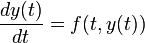
\includegraphics[scale=.6]{graphics/42ca594a14ebfe0d38675336c405ca1d.png}
% \caption{\textbackslash{}frac\{dy(t)\}\{dt\} = f(t,y(t))}
\end{figure}

with an initial value

\emph{y}(\emph{t}\textsubscript{0}) = \emph{y}\textsubscript{0}

To get a numeric solution, we replace the derivative on the LHS with a
finite difference approximation:

\begin{figure}[H]
\centering
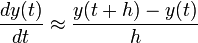
\includegraphics[scale=.6]{graphics/74ad42ba372e0541d6f14058e2c33c0f.png}
% \caption{\textbackslash{}frac\{dy(t)\}\{dt\} \textbackslash{}approx
% \textbackslash{}frac\{y(t+h)-y(t)\}\{h\}}
\end{figure}

then solve for \emph{y}(\emph{t} + \emph{h}):

\begin{figure}[H]
\centering
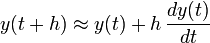
\includegraphics[scale=.6]{graphics/6ecb4a72d18052ff65e393b54c3850a2.png}
% \caption{y(t+h) \textbackslash{}approx y(t) + h \textbackslash{},
% \textbackslash{}frac\{dy(t)\}\{dt\}}
\end{figure}

which is the same as

\begin{figure}[H]
\centering
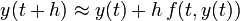
\includegraphics[scale=.6]{graphics/0a1294f5ac71c931e686c647d900fbcb.png}
% \caption{y(t+h) \textbackslash{}approx y(t) + h \textbackslash{},
% f(t,y(t))}
\end{figure}

The iterative solution rule is then:

\begin{figure}[H]
\centering
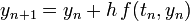
\includegraphics[scale=.6]{graphics/981cbbc69bfa735ea07313f59feba714.png}
% \caption{y\_\{n+1\} = y\_n + h \textbackslash{}, f(t\_n, y\_n)}
\end{figure}

\emph{h} is the step size, the most relevant parameter for accuracy of
the solution. A smaller step size increases accuracy but also the
computation cost, so it has always has to be hand-picked according to
the problem at hand.

\textbf{Example: Newton's Cooling Law}

Newton's cooling law describes how an object of initial temperature
\emph{T}(\emph{t}\textsubscript{0}) = \emph{T}\textsubscript{0} cools
down in an environment of temperature \emph{T}\textsubscript{\emph{R}}:

\begin{figure}[H]
\centering
\includegraphics[scale=.6]{graphics/fca99b79cfa1b2d3a65395932e824f05.png}
% \caption{\textbackslash{}frac\{dT(t)\}\{dt\} = -k \textbackslash{},
% \textbackslash{}Delta T}
\end{figure}

or

\begin{figure}[H]
\centering
\includegraphics[scale=.6]{graphics/5028ac33d1b22df1c9509179c615ce6a.png}
% \caption{\textbackslash{}frac\{dT(t)\}\{dt\} = -k \textbackslash{},
% (T(t) - T\_R)}
\end{figure}

It says that the cooling rate
\includegraphics[scale=.6]{graphics/54f43bb3bb190844c7989f5864df1b2a.png}
of the object is proportional to the current temperature difference
Δ\emph{T} = (\emph{T}(\emph{t}) − \emph{T}\textsubscript{\emph{R}}) to
the surrounding environment.

The analytical solution, which we will compare to the numerical
approximation, is

\begin{figure}[H]
\centering
\includegraphics[scale=.6]{graphics/35fc97d739522cf3dc29d28cabc2e717.png}
% \caption{T(t) = T\_R + (T\_0 - T\_R) \textbackslash{}; e\^{}\{-k t\}}
\end{figure}

\textbf{Task}

The task is to implement a routine of Euler's method and then to use it
to solve the given example of Newton's cooling law with it for three
different step sizes of 2 s, 5 s and 10 s and to compare with the
analytical solution. The initial temperature \emph{T}\textsubscript{0}
shall be 100 °C, the room temperature \emph{T}\textsubscript{\emph{R}}
20 °C, and the cooling constant \emph{k} 0.07. The time interval to
calculate shall be from 0 s to 100 s.

A reference solution (\emph{Common Lisp}) can be seen on below. We see
that bigger step sizes lead to reduced approximation accuracy.

\begin{figure}[H]
\centering
\includegraphics[scale=.6]{graphics/750px-Euler_Method_Newton_Cooling.png}
\end{figure}


\begin{wideverbatim}

(load "@lib/math.l")

(de euler (F Y A B H)
   (while (> B A)
      (prinl (round A) " " (round Y))
      (inc 'Y (*/ H (F A Y) 1.0))
      (inc 'A H) ) )

(de newtonCoolingLaw (A B)
   (*/ -0.07 (- B 20.) 1.0) )

(euler newtonCoolingLaw 100.0 0 100.0 2.0)
(euler newtonCoolingLaw 100.0 0 100.0 5.0)
(euler newtonCoolingLaw 100.0 0 100.0 10.0)

Output:

...
0.000 100.000
10.000 44.000
20.000 27.200
30.000 22.160
40.000 20.648
50.000 20.194
60.000 20.058
70.000 20.018
80.000 20.005
90.000 20.002

\end{wideverbatim}

\pagebreak{}
\section*{Evaluate binomial coefficients}

This programming task, is to calculate ANY binomial coefficient.

However, it has to be able to output
\includegraphics[scale=.6]{graphics/33a9aa45fa4dad1deffa8c921462ad74.png},
which is 10.

This formula is recommended:

\begin{figure}[H]
\centering
\includegraphics[scale=.6]{graphics/b7521c74cd98e492ade8dd3e9f40669a.png}
% \caption{\textbackslash{}binom\{n\}\{k\} =
% \textbackslash{}frac\{n!\}\{(n-k)!k!\} =
% \textbackslash{}frac\{n(n-1)(n-2)\textbackslash{}ldots(n-k+1)\}\{k(k-1)(k-2)\textbackslash{}ldots
% 1\}}
\end{figure}

\begin{wideverbatim}

(de binomial (N K)
   (let f '((N) (apply * (range 1 N)))
      (/ (f N) (* (f (- N K)) (f K))) ) )

Output:

: (binomial 5 3)
-> 10

\end{wideverbatim}

\pagebreak{}
\section*{Even or odd}

Test whether an integer is even or odd.

There is more than one way to solve this task:

\begin{itemize}
\item
  Use the even and odd predicates, if the language provides them.
\item Check the least significant digit. With binary integers, \emph{i
    \emph{bitwise-and} 1} equals 0
  \href{http://en.wiktionary.org/wiki/iff}{iff} \emph{i} is even, or
  equals 1 iff \emph{i} is odd.
\item
  Divide \emph{i} by 2. The remainder equals 0 iff \emph{i} is even. The
  remainder equals +1 or -1 iff \emph{i} is odd.
\item
  Use modular congruences:

  \begin{itemize}
  \item
    \emph{i} ≡ 0 (mod 2) iff \emph{i} is even.
  \item
    \emph{i} ≡ 1 (mod 2) iff \emph{i} is odd.
  \end{itemize}
\end{itemize}


\begin{wideverbatim}

  PicoLisp doesn't have a built-in predicate for that. Using
  '[http://software-lab.de/doc/refB.html#bit? bit?]' is the easiest
  and most efficient. The bit test with 1 will return NIL if the
  number is even.

: (bit? 1 3)
-> 1  # Odd

: (bit? 1 4)
-> NIL  # Even

\end{wideverbatim}

\pagebreak{}
\section*{Events}

\textbf{Event} is a synchronization object. An event has two states
\emph{signaled} and \emph{reset}. A \emph{task} may await for the
event to enter the desired state, usually the \emph{signaled} state.
It is released once the state is entered. Releasing waiting tasks is
called \emph{event notification}. Programmatically controlled events
can be set by a \emph{task} into one of its states.

In \emph{concurrent programming} event also refers to a notification
that some state has been reached through an asynchronous activity. The
source of the event can be:

\begin{itemize}
\item
  \emph{internal}, from another \emph{task},
  programmatically;
\item
  \emph{external}, from the hardware, such as user input, timer, etc.
  Signaling an event from the hardware is accomplished by means of
  hardware \emph{interrupts}.
\end{itemize}

Event is a low-level synchronization mechanism. It neither identify the
state that caused it signaled, nor the source of, nor who is the subject
of notification. Events augmented by data and/or publisher-subscriber
schemes are often referred as \textbf{messages}, \textbf{signals} etc.

In the context of general programming \textbf{event-driven
  architecture} refers to a design that deploy events in order to
synchronize \emph{tasks} with the asynchronous activities they must be
aware of. The opposite approach is \textbf{polling} sometimes called
\textbf{busy waiting}, when the synchronization is achieved by an
explicit periodic querying the state of the activity. As the name
suggests busy waiting consumes system resources even when the external
activity does not change its state.

Event-driven architectures are widely used in GUI design and SCADA
systems. They are flexible and have relatively short response times.
At the same time event-driven architectures suffer to the problems
related to their unpredictability. They face \emph{race condition},
deadlocking, live locks and priority inversion. For this reason
\emph{real-time} systems tend to polling schemes, trading performance
for predictability in the worst case scenario.

\begin{wideverbatim}

PicoLisp supports events from timers (via
'[http://software-lab.de/doc/refT.html#task task]' and
'[http://software-lab.de/doc/refA.html#alarm alarm]'),
file descriptors (also 'task') and various
'[http://software-lab.de/doc/refS.html#*Sig1 signals]'.
This will print a message after one second, then terminate the program after
another four seconds:

(alarm 1
   (prinl "Exit in 4 seconds")
   (alarm 4 (bye)) )

\end{wideverbatim}

\pagebreak{}
\section*{Evolutionary algorithm}

Starting with:

\begin{itemize}
\item
  The \texttt{target} string: \texttt{"METHINKS IT IS LIKE A WEASEL"}.
\item
  An array of random characters chosen from the set of upper-case
  letters together with the space, and of the same length as the target
  string. (Call it the \texttt{parent}).
\item
  A \texttt{fitness} function that computes the `closeness' of its
  argument to the target string.
\item
  A \texttt{mutate} function that given a string and a mutation rate
  returns a copy of the string, with some characters probably mutated.
\item
  While the \texttt{parent} is not yet the \texttt{target}:
\end{itemize}

\begin{itemize}
\item
  copy the \texttt{parent} C times, each time allowing some random
  probability that another character might be substituted using
  \texttt{mutate}.
\item
  Assess the \texttt{fitness} of the parent and all the copies to the
  \texttt{target} and make the most fit string the new \texttt{parent},
  discarding the others.
\item
  repeat until the parent converges, (hopefully), to the target.
\end{itemize}

Cf:
\href{http://en.wikipedia.org/wiki/Weasel\_program\#Weasel\_algorithm}{Weasel
algorithm} and
\href{http://en.wikipedia.org/wiki/Evolutionary\_algorithm}{Evolutionary
algorithm}

Note: to aid comparison, try and ensure the variables and functions
mentioned in the task description appear in solutions


\begin{wideverbatim}
This example uses 'gen', the genetic function in "lib/simul.l"

(load "@lib/simul.l")

(setq *Target (chop "METHINKS IT IS LIKE A WEASEL"))

# Generate random character
(de randChar ()
   (if (=0 (rand 0 26))
      " "
      (char (rand `(char "A") `(char "Z"))) ) )

# Fitness function (Hamming distance)
(de fitness (A)
   (cnt = A *Target) )

# Genetic algorithm
(gen
   (make                               # Parent population
      (do 100                             # C = 100 children
         (link
            (make
               (do (length *Target)
                  (link (randChar)) ) ) ) ) )
   '((A)                               # Termination condition
      (prinl (maxi fitness A))            # Print the fittest element
      (member *Target A) )                # and check if solution is found
   '((A B)                             # Recombination function
      (mapcar
         '((C D) (if (rand T) C D))       # Pick one of the chars
         A B ) )
   '((A)                               # Mutation function
      (mapcar
         '((C)
            (if (=0 (rand 0 10))          # With a proability of 10\%
               (randChar)                 # generate a new char, otherwise
               C ) )                      # return the current char
         A ) )
   fitness )                           # Selection function

Output:

RQ ASLWWWI ANSHPNABBAJ ZLTKX
DETGGNGHWITIKSXLIIEBA WAATPC
CETHINWS ITKESQGIKE A WSAGHO
METHBNWS IT NSQLIKE A WEAEWL
METHINKS IT ISCLIKE A WVASEL
METHINKS IT ISOLIKE A WEASEL
METHINKS IT IS LIKE A WEASEL

\end{wideverbatim}

\pagebreak{}
\section*{Exceptions}

\textbf{Control Structures}

These are examples of \emph{control structures}. You may also be
interested in:

\begin{itemize}
\item
  \emph{Conditional structures}
\item
  \textbf{Exceptions}
\item
  \emph{Flow-control structures}
\item
  \emph{Loops}
\end{itemize}

This task is to give an example of an exception handling routine and to
``throw'' a new exception.

Cf. \emph{Exceptions Through Nested Calls}


\begin{wideverbatim}

  [http://software-lab.de/doc/refC.html#catch catch],
  [http://software-lab.de/doc/refT.html#throw throw] (and
  [http://software-lab.de/doc/refF.html#finally finally]) can be used
  for exception handling. 'throw' will transfer control to a 'catch'
  environment that was set up with the given label.

(catch 'thisLabel          # Catch this label
   (println 1)             # Do some processing (print '1')
   (throw 'thisLabel 2)    # Abort processing and return '2'
   (println 3) )           # This is never reached

Output:

1        # '1' is printed
-> 2     # '2' is returned

\end{wideverbatim}

\pagebreak{}
\section*{Exceptions/Catch an exception thrown in a nested call}

Show how to create a user-defined exception and show how to catch an
exception raised from several nested calls away.

\begin{enumerate}
\item
  Create two user-defined exceptions, U0 and U1.
\item
  Have function foo call function bar twice.
\item
  Have function bar call function baz.
\item
  Arrange for function baz to raise, or throw exception U0 on its first
  call, then exception U1 on its second.
\item
  Function foo should catch only exception U0, not U1.
\end{enumerate}

Show/describe what happens when the program is run.


\begin{wideverbatim}

(de foo ()
   (for Tag '(U0 U1)
      (catch 'U0
         (bar Tag) ) ) )

(de bar (Tag)
   (baz Tag) )

(de baz (Tag)
   (throw Tag) )

(mapc trace '(foo bar baz))
(foo)

Output:

 foo :
  bar : U0
   baz : U0
  bar : U1
   baz : U1
[x:13] !? (throw Tag)
U1 -- Tag not found
?                          # Debug prompt

\end{wideverbatim}

\pagebreak{}
\section*{Executable library}

The general idea behind an executable library is to create a library
that when used as a library does one thing; but has the ability to be
run directly via command line. Thus the API comes with a CLI in the very
same source code file.

\textbf{Task detail}

\begin{itemize}
\item Create a library/module/dll/shared object/\ldots{} for a
  programming language that contains a function/method called
  hailstone that is a function taking a positive integer and returns
  the \emph{Hailstone sequence} for that number.
\end{itemize}

\begin{itemize}
\item The library, when executed directly should satisfy the remaining
  requirements of the \emph{Hailstone sequence} task:
\end{itemize}

2. Use the routine to show that the hailstone sequence for the number
27 has 112 elements starting with 27, 82, 41, 124 and ending with 8,
4, 2, 1

3. Show the number less than 100,000 which has the longest hailstone
sequence together with that sequences length.

\begin{itemize}
\item
  Create a second executable to calculate the following:

  \begin{itemize}
  \item
    Use the libraries hailstone function, in the standard manner, (or
    document how this use deviates from standard use of a library),
    together with extra code in this executable, to find the hailstone
    length returned most often for 1 \textless{}= n \textless{} 100,000"
  \end{itemize}
\end{itemize}

\begin{itemize}
\item
  Explain any extra setup/run steps needed to complete the task.
\end{itemize}

\textbf{Notes:}

\begin{itemize}
\item
  It is assumed that for a language that overwhelmingly ships in a
  compiled form, such as C, the library must also be an executable and
  the compiled user of that library is to do so without changing the
  compiled library. I.e. the compile tool-chain is assumed \emph{not} to
  be present in the runtime environment.
\item
  Interpreters are present in the runtime environment.
\end{itemize}


\begin{wideverbatim}

There is no formal difference between libraries and other executable files in
PicoLisp. Any function in a library can be called from the command line by
prefixing it with '-'. Create an executable file (chmod +x) "hailstone.l":

#!/usr/bin/picolisp /usr/lib/picolisp/lib.l

(de hailstone (N)
   (make
      (until (= 1 (link N))
         (setq N
            (if (bit? 1 N)
               (inc (* N 3))
               (/ N 2) ) ) ) ) )

(de hailtest ()
   (let L (hailstone 27)
      (test 112 (length L))
      (test (27 82 41 124) (head 4 L))
      (test (8 4 2 1) (tail 4 L)) )
   (let N (maxi '((N) (length (hailstone N))) (range 1 100000))
      (test 77031 N)
      (test 351 (length (hailstone N))) )
   (println 'OK)
   (bye) )

and an executable file (chmod +x) "test.l":

#!/usr/bin/picolisp /usr/lib/picolisp/lib.l

(load "hailstone.l")

(let Len NIL
   (for N 100000
      (accu 'Len (length (hailstone N)) 1) )
   (let M (maxi cdr Len)
      (prinl "The hailstone length returned most often is " (car M))
      (prinl "It is returned " (cdr M) " times") ) )
(bye)

Test:

\$ ./hailstone.l -hailtest
OK

\$ ./test.l
The hailstone length returned most often is 72
It is returned 1467 times

\end{wideverbatim}

\pagebreak{}
\section*{Execute Brain****}

\textbf{Execute Brain****} is an \textbf{implementation} of
\emph{Brainf***}. 

An implementation need only properly implement the `{[}', '{]}', `+',
'-', `\textless{}', `\textgreater{}', ',', and '.' instructions. Any
cell size is allowed, EOF support is optional, as is whether you have
bounded or unbounded memory.


\begin{wideverbatim}

This solution uses a doubly-linked list for the cell space. That list consists
of a single cell initially, and grows automatically in both directions. The
value in each cell is unlimited.

(off "Program")

(de compile (File)
   (let Stack NIL
      (setq "Program"
         (make
            (in File
               (while (char)
                  (case @
                     (">"
                        (link
                           '(setq Data
                              (or
                                 (cddr Data)
                                 (con (cdr Data) (cons 0 (cons Data))) ) ) ) )
                     ("<"
                        (link
                           '(setq Data
                              (or
                                 (cadr Data)
                                 (set (cdr Data) (cons 0 (cons NIL Data))) ) ) ) )
                     ("+" (link '(inc Data)))
                     ("-" (link '(dec Data)))
                     ("." (link '(prin (char (car Data)))))
                     ("," (link '(set Data (char (read)))))
                     ("["
                        (link
                           '(setq Code
                              ((if (=0 (car Data)) cdar cdr) Code) ) )
                        (push 'Stack (chain (cons))) )
                     ("]"
                        (unless Stack
                           (quit "Unbalanced ']'") )
                        (link
                           '(setq Code
                              ((if (n0 (car Data)) cdar cdr) Code) ) )
                        (let (There (pop 'Stack)  Here (cons There))
                           (chain (set There Here)) ) ) ) ) ) ) )
      (when Stack
         (quit "Unbalanced '['") ) ) )

(de execute ()
   (let Data (cons 0 (cons))              # Create initial cell
      (for (Code "Program"  Code)         # Run program
         (eval (pop 'Code)) )
      (while (cadr Data)                  # Find beginning of data
         (setq Data @) )
      (filter prog Data '(T NIL .)) ) )   # Return data space

\end{wideverbatim}

\begin{wideverbatim}


Output:

: (compile "hello.bf")
-> NIL

: (execute)
Goodbye, World!
-> (0 10 33 44 71 87 98 100 114 121)

\end{wideverbatim}

\pagebreak{}
\section*{Execute HQ9+}

Implement a \emph{HQ9+} interpreter or compiler for Rosetta Code.


\begin{wideverbatim}

(de hq9+ (Code)
   (let Accu 0
      (for C (chop Code)
         (case C
            ("H" (prinl "Hello, world"))
            ("Q" (prinl Code))
            ("9"
               (for (N 99 (gt0 N))
                  (prinl N " bottles of beer on the wall")
                  (prinl N " bottles of beer")
                  (prinl "Take one down, pass it around")
                  (prinl (dec 'N) " bottles of beer on the wall")
                  (prinl) ) )
            ("+" (inc 'Accu)) ) )
      Accu ) )

\end{wideverbatim}

\pagebreak{}
\section*{Execute a Markov algorithm}

Create an interpreter for a
\href{http://en.wikipedia.org/wiki/Markov\_algorithm}{Markov
  Algorithm}. Rules have the syntax:

\begin{wideverbatim}
<ruleset> ::= ((<comment> | <rule>) <newline>+)*
<comment> ::= # {<any character>}
<rule> ::= <pattern> <whitespace> -> <whitespace> [.] <replacement>
<whitespace> ::= (<tab> | <space>) [<whitespace>]
\end{wideverbatim}

There is one rule per line. If there is a . present before the
\textless{}replacement\textgreater{}, then this is a terminating rule
in which case the interpreter must halt execution. A ruleset consists
of a sequence of rules, with optional comments.


\begin{wideverbatim}

(de markov (File Text)
   (use (@A @Z R)
      (let Rules
         (make
            (in File
               (while (skip "#")
                  (when (match '(@A " " "-" ">" " " @Z) (replace (line) "@" "#"))
                     (link (cons (clip @A) (clip @Z))) ) ) ) )
         (setq Text (chop Text))
         (pack
            (loop
               (NIL
                  (find
                     '((R) (match (append '(@A) (car R) '(@Z)) Text))
                     Rules )
                  Text )
               (T (= "." (cadr (setq R @)))
                  (append @A (cddr R) @Z) )
               (setq Text (append @A (cdr R) @Z)) ) ) ) ) )

Output:

: (markov "r1" "I bought a B of As from T S.")
-> "I bought a bag of apples from my brother."

: (markov "r2" "I bought a B of As from T S.")
-> "I bought a bag of apples from T shop."

: (markov "r3" "I bought a B of As W my Bgage from T S.")
-> "I bought a bag of apples with my money from T shop."

: (markov "r4" "_1111*11111_")
-> "11111111111111111111"

: (markov "r5" "000000A000000")
-> "00011H1111000"

\end{wideverbatim}

\pagebreak{}
\section*{Execute a system command}

In this task, the goal is to run either the \texttt{ls} (\texttt{dir} on
Windows) system command, or the \texttt{pause} system command.

\begin{wideverbatim}

(call "ls")

\end{wideverbatim}

\pagebreak{}
\section*{Exponentiation operator}

Most all programming languages have a built-in implementation of
exponentiation. Re-implement integer exponentiation for both
int\textsuperscript{int} and float\textsuperscript{int} as both a
procedure, and an operator (if your language supports operator
definition).

If the language supports operator (or procedure) overloading, then an
overloaded form should be provided for both int\textsuperscript{int} and
float\textsuperscript{int} variants.


\begin{wideverbatim}

  This uses Knuth's algorithm (The Art of Computer Programming, Vol.
  2, page 442)

(de ** (X N)  # N th power of X
   (let Y 1
      (loop
         (when (bit? 1 N)
            (setq Y (* Y X)) )
         (T (=0 (setq N (>> 1 N)))
            Y )
         (setq X (* X X)) ) ) )

\end{wideverbatim}

\pagebreak{}
\section*{Extend your language}

\textbf{Control Structures}

These are examples of \emph{control structures}. You may also be
interested in:

\begin{itemize}
\item
 \emph{Conditional structures}
\item
  \emph{Exceptions}
\item
  \emph{Flow-control structures}
\item
  \emph{Loops}
\end{itemize}

Some programming languages allow you to
\href{http://en.wikipedia.org/wiki/Extensible\_programming}{extend}
the language. While this can be done to a certain degree in most
languages (e.g. by using macros), other languages go much further.
Most notably in the Forth and Lisp families, programming per se is
done by extending the language without any formal distinction between
built-in and user-defined elements.

If your language supports it, show how to introduce a new flow control
mechanism. A practical and useful example is a four-way branch:

Occasionally, code must be written that depends on \emph{two}
conditions, resulting in up to four branches (depending on whether both,
only the first, only the second, or none of the conditions are
``true''). In a C-like language this could look like the following:

\begin{verbatim}
  if (condition1isTrue) {
     if (condition2isTrue)
        bothConditionsAreTrue();
     else
        firstConditionIsTrue();
  }
  else if (condition2isTrue)
     secondConditionIsTrue();
  else
     noConditionIsTrue();
\end{verbatim}

Besides being rather cluttered, the statement(s) for `condition2isTrue'
must be written down twice. If `condition2isTrue' were a lengthy and
involved expression, it would be quite unreadable, and the code
generated by the compiler might be unnecessarily large.

This can be improved by introducing a new keyword \textbf{if2}. It is
similar to \textbf{if}, but takes two conditional statements instead of
one, and up to three `else' statements. One proposal (in pseudo-C
syntax) might be:

\begin{verbatim}
  if2 (condition1isTrue) (condition2isTrue)
     bothConditionsAreTrue();
  else1
     firstConditionIsTrue();
  else2
     secondConditionIsTrue();
  else
     noConditionIsTrue();
\end{verbatim}

Pick the syntax which suits your language. The keywords `else1' and
`else2' are just examples. The new conditional expression should look,
nest and behave analog to the language's built-in `if' statement.


\begin{wideverbatim}

(undef 'if2)  # Undefine the built-in 'if2'

(de if2 "P"
   (if (eval (pop '"P"))
      (eval ((if (eval (car "P")) cadr caddr) "P"))
      (if (eval (car "P"))
         (eval (cadddr "P"))
         (run (cddddr "P")) ) ) )

Usage:

(if2 (condition1isTrue) (condition2isTrue)
   (bothConditionsAreTrue)             # A single expression in each of the
   (firstConditionIsTrue)              # first three branches
   (secondConditionIsTrue)
   (noConditionIsTrue)                 # The final branch may contain
   (...) )                             # an arbitrary number of expressions

As another example of language extension, see [[Anonymous recursion#PicoLisp]].

\end{wideverbatim}

\pagebreak{}
\section*{Extreme floating point values}

The IEEE floating point specification defines certain `extreme' floating
point values such as minus zero, -0.0, a value distinct from plus zero;
not a number, NaN; and plus and minus infinity.

The task is to use expressions involving other `normal' floating point
values in your language to calculate these, (and maybe other), extreme
floating point values in your language and assign them to variables.
Print the values of these variables if possible; and show some
arithmetic with these values and variables. If your language can
directly enter these extreme floating point values then show it.

C.f:

\begin{itemize}
\item
  \href{http://www-users.math.umd.edu/~jkolesar/mait613/floating\_point\_math.pdf}{What
  Every Computer Scientist Should Know About Floating-Point Arithmetic}
\item
  \emph{Infinity}
\item
  \emph{Detect division by zero}
\item
  \emph{Literals/Floating point}
\end{itemize}


\begin{wideverbatim}

  PicoLisp has only very limited built-in floating point support, and
  handles the rest by calling native (typically C) libraries. Minus
  zero and negative infinity cannot be represented, while NaN is
  represented by NIL

(load "@lib/math.l")

: (exp 1000.0)  # Too large for IEEE floats
-> T

: (+ 1 2 NIL 3)  # NaN propagates
-> NIL

\end{wideverbatim}



% %%%%%%%%%%%%%%%%%%%%%%%% referenc.tex %%%%%%%%%%%%%%%%%%%%%%%%%%%%%%
% sample references
% %
% Use this file as a template for your own input.
%
%%%%%%%%%%%%%%%%%%%%%%%% Springer-Verlag %%%%%%%%%%%%%%%%%%%%%%%%%%
%
% BibTeX users please use
% \bibliographystyle{}
% \bibliography{}
%
\biblstarthook{In view of the parallel print and (chapter-wise) online publication of your book at \url{www.springerlink.com} it has been decided that -- as a genreral rule --  references should be sorted chapter-wise and placed at the end of the individual chapters. However, upon agreement with your contact at Springer you may list your references in a single seperate chapter at the end of your book. Deactivate the class option \texttt{sectrefs} and the \texttt{thebibliography} environment will be put out as a chapter of its own.\\\indent
References may be \textit{cited} in the text either by number (preferred) or by author/year.\footnote{Make sure that all references from the list are cited in the text. Those not cited should be moved to a separate \textit{Further Reading} section or chapter.} The reference list should ideally be \textit{sorted} in alphabetical order -- even if reference numbers are used for the their citation in the text. If there are several works by the same author, the following order should be used: 
\begin{enumerate}
\item all works by the author alone, ordered chronologically by year of publication
\item all works by the author with a coauthor, ordered alphabetically by coauthor
\item all works by the author with several coauthors, ordered chronologically by year of publication.
\end{enumerate}
The \textit{styling} of references\footnote{Always use the standard abbreviation of a journal's name according to the ISSN \textit{List of Title Word Abbreviations}, see \url{http://www.issn.org/en/node/344}} depends on the subject of your book:
\begin{itemize}
\item The \textit{two} recommended styles for references in books on \textit{mathematical, physical, statistical and computer sciences} are depicted in ~\cite{science-contrib, science-online, science-mono, science-journal, science-DOI} and ~\cite{phys-online, phys-mono, phys-journal, phys-DOI, phys-contrib}.
\item Examples of the most commonly used reference style in books on \textit{Psychology, Social Sciences} are~\cite{psysoc-mono, psysoc-online,psysoc-journal, psysoc-contrib, psysoc-DOI}.
\item Examples for references in books on \textit{Humanities, Linguistics, Philosophy} are~\cite{humlinphil-journal, humlinphil-contrib, humlinphil-mono, humlinphil-online, humlinphil-DOI}.
\item Examples of the basic Springer style used in publications on a wide range of subjects such as \textit{Computer Science, Economics, Engineering, Geosciences, Life Sciences, Medicine, Biomedicine} are ~\cite{basic-contrib, basic-online, basic-journal, basic-DOI, basic-mono}. 
\end{itemize}
}

\begin{thebibliography}{99.}%
% and use \bibitem to create references.
%
% Use the following syntax and markup for your references if 
% the subject of your book is from the field 
% "Mathematics, Physics, Statistics, Computer Science"
%
% Contribution 
\bibitem{science-contrib} Broy, M.: Software engineering --- from auxiliary to key technologies. In: Broy, M., Dener, E. (eds.) Software Pioneers, pp. 10-13. Springer, Heidelberg (2002)
%
% Online Document
\bibitem{science-online} Dod, J.: Effective substances. In: The Dictionary of Substances and Their Effects. Royal Society of Chemistry (1999) Available via DIALOG. \\
\url{http://www.rsc.org/dose/title of subordinate document. Cited 15 Jan 1999}
%
% Monograph
\bibitem{science-mono} Geddes, K.O., Czapor, S.R., Labahn, G.: Algorithms for Computer Algebra. Kluwer, Boston (1992) 
%
% Journal article
\bibitem{science-journal} Hamburger, C.: Quasimonotonicity, regularity and duality for nonlinear systems of partial differential equations. Ann. Mat. Pura. Appl. \textbf{169}, 321--354 (1995)
%
% Journal article by DOI
\bibitem{science-DOI} Slifka, M.K., Whitton, J.L.: Clinical implications of dysregulated cytokine production. J. Mol. Med. (2000) doi: 10.1007/s001090000086 
%
\bigskip

% Use the following (APS) syntax and markup for your references if 
% the subject of your book is from the field 
% "Mathematics, Physics, Statistics, Computer Science"
%
% Online Document
\bibitem{phys-online} J. Dod, in \textit{The Dictionary of Substances and Their Effects}, Royal Society of Chemistry. (Available via DIALOG, 1999), 
\url{http://www.rsc.org/dose/title of subordinate document. Cited 15 Jan 1999}
%
% Monograph
\bibitem{phys-mono} H. Ibach, H. L\"uth, \textit{Solid-State Physics}, 2nd edn. (Springer, New York, 1996), pp. 45-56 
%
% Journal article
\bibitem{phys-journal} S. Preuss, A. Demchuk Jr., M. Stuke, Appl. Phys. A \textbf{61}
%
% Journal article by DOI
\bibitem{phys-DOI} M.K. Slifka, J.L. Whitton, J. Mol. Med., doi: 10.1007/s001090000086
%
% Contribution 
\bibitem{phys-contrib} S.E. Smith, in \textit{Neuromuscular Junction}, ed. by E. Zaimis. Handbook of Experimental Pharmacology, vol 42 (Springer, Heidelberg, 1976), p. 593
%
\bigskip
%
% Use the following syntax and markup for your references if 
% the subject of your book is from the field 
% "Psychology, Social Sciences"
%
%
% Monograph
\bibitem{psysoc-mono} Calfee, R.~C., \& Valencia, R.~R. (1991). \textit{APA guide to preparing manuscripts for journal publication.} Washington, DC: American Psychological Association.
%
% Online Document
\bibitem{psysoc-online} Dod, J. (1999). Effective substances. In: The dictionary of substances and their effects. Royal Society of Chemistry. Available via DIALOG. \\
\url{http://www.rsc.org/dose/Effective substances.} Cited 15 Jan 1999.
%
% Journal article
\bibitem{psysoc-journal} Harris, M., Karper, E., Stacks, G., Hoffman, D., DeNiro, R., Cruz, P., et al. (2001). Writing labs and the Hollywood connection. \textit{J Film} Writing, 44(3), 213--245.
%
% Contribution 
\bibitem{psysoc-contrib} O'Neil, J.~M., \& Egan, J. (1992). Men's and women's gender role journeys: Metaphor for healing, transition, and transformation. In B.~R. Wainrig (Ed.), \textit{Gender issues across the life cycle} (pp. 107--123). New York: Springer.
%
% Journal article by DOI
\bibitem{psysoc-DOI}Kreger, M., Brindis, C.D., Manuel, D.M., Sassoubre, L. (2007). Lessons learned in systems change initiatives: benchmarks and indicators. \textit{American Journal of Community Psychology}, doi: 10.1007/s10464-007-9108-14.
%
%
% Use the following syntax and markup for your references if 
% the subject of your book is from the field 
% "Humanities, Linguistics, Philosophy"
%
\bigskip
%
% Journal article
\bibitem{humlinphil-journal} Alber John, Daniel C. O'Connell, and Sabine Kowal. 2002. Personal perspective in TV interviews. \textit{Pragmatics} 12:257--271
%
% Contribution 
\bibitem{humlinphil-contrib} Cameron, Deborah. 1997. Theoretical debates in feminist linguistics: Questions of sex and gender. In \textit{Gender and discourse}, ed. Ruth Wodak, 99--119. London: Sage Publications.
%
% Monograph
\bibitem{humlinphil-mono} Cameron, Deborah. 1985. \textit{Feminism and linguistic theory.} New York: St. Martin's Press.
%
% Online Document
\bibitem{humlinphil-online} Dod, Jake. 1999. Effective substances. In: The dictionary of substances and their effects. Royal Society of Chemistry. Available via DIALOG. \\
http://www.rsc.org/dose/title of subordinate document. Cited 15 Jan 1999
%
% Journal article by DOI
\bibitem{humlinphil-DOI} Suleiman, Camelia, Daniel C. O�Connell, and Sabine Kowal. 2002. `If you and I, if we, in this later day, lose that sacred fire...�': Perspective in political interviews. \textit{Journal of Psycholinguistic Research}. doi: 10.1023/A:1015592129296.
%
%
%
\bigskip
%
%
% Use the following syntax and markup for your references if 
% the subject of your book is from the field 
% "Computer Science, Economics, Engineering, Geosciences, Life Sciences"
%
%
% Contribution 
\bibitem{basic-contrib} Brown B, Aaron M (2001) The politics of nature. In: Smith J (ed) The rise of modern genomics, 3rd edn. Wiley, New York 
%
% Online Document
\bibitem{basic-online} Dod J (1999) Effective Substances. In: The dictionary of substances and their effects. Royal Society of Chemistry. Available via DIALOG. \\
\url{http://www.rsc.org/dose/title of subordinate document. Cited 15 Jan 1999}
%
% Journal article by DOI
\bibitem{basic-DOI} Slifka MK, Whitton JL (2000) Clinical implications of dysregulated cytokine production. J Mol Med, doi: 10.1007/s001090000086
%
% Journal article
\bibitem{basic-journal} Smith J, Jones M Jr, Houghton L et al (1999) Future of health insurance. N Engl J Med 965:325--329
%
% Monograph
\bibitem{basic-mono} South J, Blass B (2001) The future of modern genomics. Blackwell, London 
%
\end{thebibliography}


%%%%%%%%%%%%%%%%%%%%% chapter.tex %%%%%%%%%%%%%%%%%%%%%%%%%%%%%%%%%
%
% sample chapter
%
% Use this file as a template for your own input.
%
%%%%%%%%%%%%%%%%%%%%%%%% Springer-Verlag %%%%%%%%%%%%%%%%%%%%%%%%%%
%\motto{Use the template \emph{chapter.tex} to style the various elements of your chapter content.}

\chapter{Rosetta Code Tasks starting with F}

\section*{Factorial}

The \textbf{Factorial Function} of a positive integer, \emph{n}, is
defined as the product of the sequence \emph{n}, \emph{n}-1, \emph{n}-2,
\ldots{}1 and the factorial of zero, 0, is
\href{http://en.wikipedia.org/wiki/Factorial\#Definition}{defined} as
being 1.

Write a function to return the factorial of a number. Solutions can be
iterative or recursive. Support for trapping negative n errors is
optional.

\begin{wideverbatim}

(de fact (N)
   (if (=0 N)
      1
      (* N (fact (dec N))) ) )

or

(de fact (N)
   (apply * (range 1 N)) )

\end{wideverbatim}

\pagebreak{}
\section*{Factors of a Mersenne number}

A Mersenne number is a number in the form of 2\textsuperscript{P}-1.
If P is prime, the Mersenne number may be a Mersenne prime (if P is
not prime, the Mersenne number is also not prime). In the search for
Mersenne prime numbers it is advantageous to eliminate exponents by
finding a small factor before starting a, potentially lengthy,
\emph{Lucas-Lehmer test}. There are very efficient algorithms for
determining if a number divides 2\textsuperscript{P}-1 (or
equivalently, if 2\textsuperscript{P} mod (the number) = 1). Some
languages already have built-in implementations of this
exponent-and-mod operation (called \emph{modPow} or similar). The
following is how to implement this \emph{modPow} yourself:

For example, let's compute 2\textsuperscript{23} mod 47. Convert the
exponent 23 to binary, you get 10111. Starting with \texttt{square} = 1,
repeatedly square it. Remove the top bit of the exponent, and if it's 1
multiply \texttt{square} by the base of the exponentiation (2), then
compute \texttt{square} modulo 47. Use the result of the modulo from the
last step as the initial value of \texttt{square} in the next step:

\begin{verbatim}
                 Remove   Optional   
   square        top bit  multiply by 2  mod 47
   ------------  -------  -------------  ------
   1*1 = 1       1  0111  1*2 = 2           2
   2*2 = 4       0   111     no             4
   4*4 = 16      1    11  16*2 = 32        32
   32*32 = 1024  1     1  1024*2 = 2048    27
   27*27 = 729   1        729*2 = 1458      1
\end{verbatim}

Since 2\textsuperscript{23} mod 47 = 1, 47 is a factor of
2\textsuperscript{P}-1. (To see this, subtract 1 from both sides:
2\textsuperscript{23}-1 = 0 mod 47.) Since we've shown that 47 is a
factor, 2\textsuperscript{23}-1 is not prime. Further properties of
Mersenne numbers allow us to refine the process even more. Any factor
q of 2\textsuperscript{P}-1 must be of the form 2kP+1, k being a
positive integer or zero. Furthermore, q must be 1 or 7 mod 8. Finally
any potential factor q must be \emph{prime}. As in other trial
division algorithms, the algorithm stops when 2kP+1 \textgreater{}
sqrt(N).

These primality tests only work on Mersenne numbers where P is prime.
For example, M\textsubscript{4}=15 yields no factors using these
techniques, but factors into 3 and 5, neither of which fit 2kP+1.

\textbf{Task:} Using the above method find a factor of
2\textsuperscript{929}-1 (aka M929)


\begin{wideverbatim}

(de **Mod (X Y N)
   (let M 1
      (loop
         (when (bit? 1 Y)
            (setq M (\% (* M X) N)) )
         (T (=0 (setq Y (>> 1 Y)))
            M )
         (setq X (\% (* X X) N)) ) ) )

(de prime? (N)
   (or
      (= N 2)
      (and
         (> N 1)
         (bit? 1 N)
         (for (D 3  T  (+ D 2))
            (T (> D (sqrt N)) T)
            (T (=0 (\% N D)) NIL) ) ) ) )

(de mFactor (P)
   (let (Lim (sqrt (dec (** 2 P)))  K 0  Q)
      (loop
         (setq Q (inc (* 2 (inc 'K) P)))
         (T (>= Q Lim) NIL)
         (T
            (and
               (member (\% Q 8) (1 7))
               (prime? Q)
               (= 1 (**Mod 2 P Q)) )
            Q ) ) ) )

\end{wideverbatim}

\begin{wideverbatim}


Output:

: (for P (2 3 4 5 7 11 13 17 19 23 29 31 37 41 43 47 53 929)
   (prinl
      "M" P " = 2**" P "-1 is "
      (cond
         ((not (prime? P)) "not prime")
         ((mFactor P) (pack "composite with factor " @))
         (T "prime") ) ) )
M2 = 2**2-1 is prime
M3 = 2**3-1 is prime
M4 = 2**4-1 is not prime
M5 = 2**5-1 is prime
M7 = 2**7-1 is prime
M11 = 2**11-1 is composite with factor 23
M13 = 2**13-1 is prime
M17 = 2**17-1 is prime
M19 = 2**19-1 is prime
M23 = 2**23-1 is composite with factor 47
M29 = 2**29-1 is composite with factor 233
M31 = 2**31-1 is prime
M37 = 2**37-1 is composite with factor 223
M41 = 2**41-1 is composite with factor 13367
M43 = 2**43-1 is composite with factor 431
M47 = 2**47-1 is composite with factor 2351
M53 = 2**53-1 is composite with factor 6361
M929 = 2**929-1 is composite with factor 13007

\end{wideverbatim}

\pagebreak{}
\section*{Factors of an integer}

\textbf{Basic Data Operation}\\ This is a basic data operation. It
represents a fundamental action on a basic data type.

You may see other such operations in the \emph{Basic Data Operations}
category, or:

\textbf{Integer Operations} \\
\emph{Arithmetic} \textbar{} \emph{Comparison}

\textbf{Boolean Operations} \\ \emph{Bitwise} \textbar{}
\emph{Logical}

\textbf{String Operations} \\
\emph{Concatenation} \textbar{} \emph{Interpolation} \textbar{}
\emph{Matching}

\textbf{Memory Operations} \\
\emph{Pointers \& references} \textbar{} \emph{Addresses}

Compute the \href{http://en.wikipedia.org/wiki/Divisor}{factors} of a
positive integer. These factors are the positive integers by which the
number being factored can be divided to yield a positive integer result
(though the concepts function correctly for zero and negative integers,
the set of factors of zero is has countably infinite members, and the
factors of negative integers can be obtained from the factors of related
positive numbers without difficulty; this task does not require handling
of either of these cases). Note that even prime numbers will have at
least two factors; `1' and themselves.

See also:

\begin{itemize}
\item
  \emph{Prime decomposition}
\end{itemize}


\begin{wideverbatim}

(de factors (N)
   (filter
      '((D) (=0 (% N D)))
      (range 1 N) ) )
\end{wideverbatim}

\pagebreak{}
\section*{Fast Fourier transform}

The purpose of this task is to calculate the FFT (Fast Fourier
Transform) of an input sequence. The most general case allows for
complex numbers at the input and results in a sequence of equal length,
again of complex numbers. If you need to restrict yourself to real
numbers the output should be the magnitude (i.e. sqrt(re²+im²)) of the
complex result. The classic version is the recursive Cooley--Tukey FFT.
\href{http://en.wikipedia.org/wiki/Cooley--Tukey\_FFT\_algorithm}{Wikipedia}
has pseudocode for that. Further optimizations are possible but not
required.


\begin{wideverbatim}

{{works with|PicoLisp|3.1.0.3}}

# apt-get install libfftw3-dev

(scl 4)

(de FFTW_FORWARD . -1)
(de FFTW_ESTIMATE . 64)

(de fft (Lst)
   (let
      (Len (length Lst)
         In (native "libfftw3.so" "fftw_malloc" 'N (* Len 16))
         Out (native "libfftw3.so" "fftw_malloc" 'N (* Len 16))
         P (native "libfftw3.so" "fftw_plan_dft_1d" 'N
            Len In Out FFTW_FORWARD FFTW_ESTIMATE ) )
      (struct In NIL (cons 1.0 (apply append Lst)))
      (native "libfftw3.so" "fftw_execute" NIL P)
      (prog1 (struct Out (make (do Len (link (1.0 . 2)))))
         (native "libfftw3.so" "fftw_destroy_plan" NIL P)
         (native "libfftw3.so" "fftw_free" NIL Out)
         (native "libfftw3.so" "fftw_free" NIL In) ) ) )

Test:

(for R (fft '((1.0 0) (1.0 0) (1.0 0) (1.0 0) (0 0) (0 0) (0 0) (0 0)))
   (tab (6 8)
      (round (car R))
      (round (cadr R)) ) )

Output:

 4.000   0.000
 1.000  -2.414
 0.000   0.000
 1.000  -0.414
 0.000   0.000
 1.000   0.414
 0.000   0.000
 1.000   2.414

\end{wideverbatim}

\pagebreak{}
\section*{Fibonacci n-step number sequences}

These number series are an expansion of the ordinary
\emph{Fibonacci sequence} where:


The \textbf{Fibonacci sequence} is a sequence F\textsubscript{n} of
natural numbers defined recursively:

\begin{verbatim}
F0 = 0
F1 = 1
Fn = Fn-1 + Fn-2, if n>1
\end{verbatim}

Write a function to generate the nth Fibonacci number. Solutions can be
iterative or recursive (though recursive solutions are generally
considered too slow and are mostly used as an exercise in recursion).

The sequence is sometimes extended into negative numbers by using a
straightforward inverse of the positive definition:

\begin{verbatim}
Fn = Fn+2 - Fn+1, if n<0
\end{verbatim}

Support for negative n in the solution is optional.

\begin{description}
\item[Cf.]
\end{description}

\begin{itemize}
\item \emph{Fibonacci n-step number sequences‎}
\end{itemize}

\begin{description}
\item[References]
\end{description}

\begin{itemize}
\item
  \href{http://en.wikipedia.org/wiki/Fibonacci\_number}{Wikipedia,
  Fibonacci number}
\item
  \href{http://en.wikipedia.org/wiki/Lucas\_number}{Wikipedia, Lucas
  number}
\item
  \href{http://mathworld.wolfram.com/FibonacciNumber.html}{MathWorld,
  Fibonacci Number}
\item
  \href{http://www.math-cs.ucmo.edu/~curtisc/articles/howardcooper/genfib4.pdf}{Some
  identities for r-Fibonacci numbers}
\item
  \href{http://oeis.org/A000045}{OEIS Fibonacci numbers}
\item
  \href{http://oeis.org/A000032}{OEIS Lucas numbers}
\end{itemize}



\begin{enumerate}
\item
  For \emph{n} = 2 we have the Fibonacci sequence; with initial values
  {[}1,1{]} and
  \begin{figure}[H]
    \centering
    \includegraphics[scale=.6]{graphics/ea8fba6081e51a2e4f0cd0d58c3c7032.png}    
  \end{figure}
\item
  For \emph{n} = 3 we have the tribonacci sequence; with initial values
  {[}1,1,2{]} and
  \begin{figure}[H]
    \centering
     \includegraphics[scale=.6]{graphics/a96e7fe6a7eb7371ab85f6a135b84056.png}    
  \end{figure}
\item
  For \emph{n} = 4 we have the tetranacci sequence; with initial values
  {[}1,1,2,4{]} and
  \begin{figure}[H]
    \centering
    \includegraphics[scale=.6]{graphics/ea2b3ddffa2a578dbe5d923abd914aa5.png}
  \end{figure}

\ldots{}    

\item
  For general \emph{n} \textgreater{} 2 we have the Fibonacci
  \emph{n}-step sequence -
  \includegraphics[scale=.6]{graphics/f6e22469b4396d8fa34e202e5c716abc.png};
  with initial values of the first \emph{n} values of the (\emph{n} −
  1)'th Fibonacci \emph{n}-step sequence
  \includegraphics[scale=.6]{graphics/79293ba1053dbc3f23c579b2e8141034.png};
  and \emph{k}'th value of this \emph{n}'th sequence being

  \begin{figure}[H]
    \centering
     \includegraphics[scale=.6]{graphics/c53daded435e185afefbac417fef75e7.png}    
  \end{figure}
\end{enumerate}

For small values of \emph{n},
\href{http://en.wikipedia.org/wiki/Number\_prefix\#Greek\_series}{Greek
numeric prefixes} are sometimes used to individually name each series.

\ctable[caption = { Fibonacci \emph{n}-step sequences },
pos = H, center, botcap]{lll}
{% notes
}
{% rows
\FL
\emph{n} & Series name & Values
\ML
2 & fibonacci & 1 1 2 3 5 8 13 21 34 55 89 144 233 377 610 \ldots{}
\\\noalign{\medskip}
3 & tribonacci & 1 1 2 4 7 13 24 44 81 149 274 504 927 1705 3136
\ldots{}
\\\noalign{\medskip}
4 & tetranacci & 1 1 2 4 8 15 29 56 108 208 401 773 1490 2872 5536
\ldots{}
\\\noalign{\medskip}
5 & pentanacci & 1 1 2 4 8 16 31 61 120 236 464 912 1793 3525 6930
\ldots{}
\\\noalign{\medskip}
6 & hexanacci & 1 1 2 4 8 16 32 63 125 248 492 976 1936 3840 7617
\ldots{}
\\\noalign{\medskip}
7 & heptanacci & 1 1 2 4 8 16 32 64 127 253 504 1004 2000 3984 7936
\ldots{}
\\\noalign{\medskip}
8 & octonacci & 1 1 2 4 8 16 32 64 128 255 509 1016 2028 4048 8080
\ldots{}
\\\noalign{\medskip}
9 & nonanacci & 1 1 2 4 8 16 32 64 128 256 511 1021 2040 4076 8144
\ldots{}
\\\noalign{\medskip}
10 & decanacci & 1 1 2 4 8 16 32 64 128 256 512 1023 2045 4088 8172
\ldots{}
\LL
}

Allied sequences can be generated where the initial values are changed:

\textbf{The \href{http://en.wikipedia.org/wiki/Lucas\_number}{Lucas
series}} sums the two preceeding values like the fibonacci series for
\emph{n} = 2 but uses {[}2,1{]} as its initial values.

\pagebreak{}
\begin{description}
\item[The task is to]
\end{description}

\begin{enumerate}
\item
  Write a function to generate Fibonacci \emph{n}-step number sequences
  given its initial values and assuming the number of initial values
  determines how many previous values are summed to make the next number
  of the series.
\item
  Use this to print and show here at least the first ten members of the
  Fibo/tribo/tetra-nacci and Lucas sequences.
\end{enumerate}

\begin{description}
\item[Cf.]
\end{description}

\begin{itemize}
\item \emph{Fibonacci sequence}
\item
  \href{http://mathworld.wolfram.com/Fibonaccin-StepNumber.html}{Wolfram
  Mathworld}
\item \emph{Hofstadter Q sequence‎}
\end{itemize}


\begin{wideverbatim}

(de nacci (Init Cnt)
   (let N (length Init)
      (make
         (made Init)
         (do (- Cnt N)
            (link (apply + (tail N (made)))) ) ) ) )

Test:
# Fibonacci
: (nacci (1 1) 10)
-> (1 1 2 3 5 8 13 21 34 55)

# Tribonacci
: (nacci (1 1 2) 10)
-> (1 1 2 4 7 13 24 44 81 149)

# Tetranacci
: (nacci (1 1 2 4) 10)
-> (1 1 2 4 8 15 29 56 108 208)

# Lucas
: (nacci (2 1) 10)
-> (2 1 3 4 7 11 18 29 47 76)

# Decanacci
: (nacci (1 1 2 4 8 16 32 64 128 256) 15)
-> (1 1 2 4 8 16 32 64 128 256 512 1023 2045 4088 8172)

\end{wideverbatim}

\pagebreak{}
\section*{Fibonacci sequence}

The \textbf{Fibonacci sequence} is a sequence F\textsubscript{n} of
natural numbers defined recursively:

\begin{verbatim}
F0 = 0
F1 = 1
Fn = Fn-1 + Fn-2, if n>1
\end{verbatim}

Write a function to generate the nth Fibonacci number. Solutions can be
iterative or recursive (though recursive solutions are generally
considered too slow and are mostly used as an exercise in recursion).

The sequence is sometimes extended into negative numbers by using a
straightforward inverse of the positive definition:

\begin{verbatim}
Fn = Fn+2 - Fn+1, if n<0
\end{verbatim}

Support for negative n in the solution is optional.

\begin{description}
\item[Cf.]
\end{description}

\begin{itemize}
\item \emph{Fibonacci n-step number sequences‎}
\end{itemize}

\begin{description}
\item[References]
\end{description}

\begin{itemize}
\item
  \href{http://en.wikipedia.org/wiki/Fibonacci\_number}{Wikipedia,
  Fibonacci number}
\item
  \href{http://en.wikipedia.org/wiki/Lucas\_number}{Wikipedia, Lucas
  number}
\item
  \href{http://mathworld.wolfram.com/FibonacciNumber.html}{MathWorld,
  Fibonacci Number}
\item
  \href{http://www.math-cs.ucmo.edu/~curtisc/articles/howardcooper/genfib4.pdf}{Some
  identities for r-Fibonacci numbers}
\item
  \href{http://oeis.org/A000045}{OEIS Fibonacci numbers}
\item
  \href{http://oeis.org/A000032}{OEIS Lucas numbers}
\end{itemize}


\begin{wideverbatim}

Recursive

(de fibo (N)
   (if (> 2 N)
      1
      (+ (fibo (dec N)) (fibo (- N 2))) ) )

Recursive with Cache

Using a recursive version doesn't need to be slow, as the following shows:

(de fibo (N)
   (cache '(NIL) (pack (char (hash N)) N)  # Use a cache to accelerate
      (if (> 2 N)
         N
         (+ (fibo (dec N)) (fibo (- N 2))) ) ) )

(bench (fibo 1000))

Output:

0.012 sec
-> 43466557686937456435688527675040625802564660517371780402481729089536555417949
05189040387984007925516929592259308032263477520968962323987332247116164299644090
6533187938298969649928516003704476137795166849228875

\end{wideverbatim}

\pagebreak{}
\section*{File IO}


\textbf{File IO} is part of \emph{Short Circuit}'s
\textbf{\href{/wiki/Category:Selection/Short\_Circuit/Console\_Program\_Basics}{Console
    Program Basics}} selection.

In this task, the job is to create a file called ``output.txt'', and
place in it the contents of the file ``input.txt'', \emph{via an
intermediate variable.} In other words, your program will demonstrate:
(1) how to read from a file into a variable, and (2) how to write a
variable's contents into a file. Oneliners that skip the intermediate
variable are of secondary interest --- operating systems have copy
commands for that.

\begin{wideverbatim}

# Using a variable

(let V (in "input.txt" (till))
   (out "output.txt" (prin V)) )

# Skipping intermediate variable

(in "input.txt"
   (out "output.txt"
      (echo) ) )

\end{wideverbatim}

\pagebreak{}
\section*{File modification time}

This task will attempt to get and set the modification time of a file.

\begin{wideverbatim}

(let File "test.file"
   (and
      (info File)
      (prinl (stamp (cadr @) (cddr @))) ) # Print date and time in UTC
   (call 'touch File) )                   # Set modification time to "now"

\end{wideverbatim}

\pagebreak{}
\section*{File size}

In this task, the job is to verify the size of a file called
``input.txt'' for a file in the current working directory and another
one in the file system root.

\begin{wideverbatim}

(println (car (info "input.txt")))
(println (car (info "/input.txt")))

\end{wideverbatim}

\pagebreak{}
\section*{Filter}

Select certain elements from an Array into a new Array in a generic way.
To demonstrate, select all even numbers from an Array.

As an option, give a second solution which filters destructively, by
modifying the original Array rather than creating a new Array.

\begin{wideverbatim}

(filter '((N) (not (bit? 1 N)))
   (1 2 3 4 5 6 7 8 9) )

Output:

-> (2 4 6 8)

\end{wideverbatim}

\pagebreak{}
\section*{Find Common Directory Path}

Create a routine that, given a set of strings representing directory
paths and a single character directory separator, will return a string
representing that part of the directory tree that is common to all the
directories.

Test your routine using the forward slash `/' character as the directory
separator and the following three strings as input paths:

\begin{verbatim}
 '/home/user1/tmp/coverage/test'
 '/home/user1/tmp/covert/operator'
 '/home/user1/tmp/coven/members'
\end{verbatim}

Note: The resultant path should be the valid directory
\texttt{'/home/user1/tmp'} and not the longest common string
\texttt{'/home/user1/tmp/cove'}.

If your language has a routine that performs this function (even if it
does not have a changeable separator character, then mention it as
part of the task)

\begin{wideverbatim}

(de commonPath (Lst Chr)
   (glue Chr
      (make
         (apply find
            (mapcar '((L) (split (chop L) Chr)) Lst)
            '(@ (or (pass <>) (nil (link (next))))) ) ) ) )

Output:

(commonPath
   (quote
      "/home/user1/tmp/coverage/test"
      "/home/user1/tmp/covert/operator"
      "/home/user1/tmp/coven/members" )
   "/" )

-> "/home/user1/tmp"

\end{wideverbatim}

\pagebreak{}
\section*{Find first and last set bit of a long integer}

\emph{Clarification: This task is asking for the position of two bits in
the binary representation of a positive integer. Some parts of this task
assume that this is the native representation in the language you are
working in. Any part of this task which makes assumptions about native
representation should be treated as a recommendation which is only
relevant in some contexts. A bit is defined as the exponent in a binary
polynomial -- an exponent corresponding to a power of 2 which has a
non-zero multiplier in the summation sequence of powers of two which
yields the desired positive integer, where the only allowed coefficients
are 0 and 1.}

Define routines (or operators) \textbf{lwb} and \textbf{upb} that find
the \emph{first} and \emph{last} set bit in a binary value. Implement
using a binary search to find the location of the particular upper/lower
bit.

Also: Define the reverse routines (or operators) \textbf{rlwb} and
\textbf{rupb} that find host's \emph{positive integers} least- and
most-significant set bit in a binary value expressed in
\href{http://en.wikipedia.org/wiki/Bit\_numbering\#LSB\_0\_bit\_numbering}{LSB
0 bit numbering}, i.e. indexed from the extreme right bit.

Use primarily \textbf{bit} operations, such as \textbf{and},
\textbf{or}, and bit shifting. Avoid additions, multiplications and
especially avoid divisions.

\textbf{Two implementations:}

\begin{enumerate}
\item
  For the host word size on the host platform, implement the routine
  ``efficiently'' in without looping or recursion.
\item
  For the extended precision/long word implement the algorithm more
  generally - maybe as a template, and maybe with looping - so that any
  \emph{bits width} for a binary type can be accommodated.
\end{enumerate}

\textbf{Test cases:}

\begin{enumerate}
\item
  For the host machine word size: Use the powers of 42 up to host's the
  ``natural'' word size to calculate the index of the first and last set
  bit.
\item
  For the extended precision: Use the powers of 1302 up to the host's
  next ``natural'' \textbf{long} host \emph{word} size to calculate the
  index of the first and last set bit.
\item
  Output bit indexes in
  \href{http://en.wikipedia.org/wiki/Bit\_numbering\#LSB\_0\_bit\_numbering}{LSB
  0 bit numbering}.
\end{enumerate}

\textbf{Additionally:}

In a particular language, there maybe (at least) two alternative
approaches of calculating the required values:

\begin{itemize}
\item
  Using an external library.
\item
  Using a built-in library.
\end{itemize}

If any of these approaches are available, then \emph{also} note the
library or built-in name.

\textbf{See also:}

\begin{itemize}
\item
  \href{http://graphics.stanford.edu/~seander/bithacks.html\#IntegerLog}{Find
  the log base 2 of an N-bit integer in O(lg(N)) operations}
\item
  \href{http://pdos.csail.mit.edu/6.858/2011/readings/i386/BSF.htm}{80386
  Instruction Set - BSF -- Bit Scan Forward}
\end{itemize}



\begin{wideverbatim}

(de msb (N)
   (dec (length (bin (abs N)))) )

(de lsb (N)
   (length (stem (chop (bin N)) "1")) )

Test:

(for N (1 42 717368321110468608 291733167875766667063796853374976)
   (tab (33 6 6) N (lsb N) (msb N)) )

Output:

                                1     0     0
                               42     1     5
               717368321110468608    11    59
291733167875766667063796853374976    20   107

\end{wideverbatim}

\pagebreak{}
\section*{Find limit of recursion}

\textbf{Find limit of recursion} is part of \emph{Short Circuit}'s
\textbf{\emph{Console Program Basics}} selection.

Find the limit of recursion.

\begin{wideverbatim}

  The 64-bit and the 32-bit version behave slightly different. While
  the 32-bit version imposes no limit on its own, and relies on the
  'ulimit' setting of the caller, the 64-bit version segments the
  available stack (likewise depending on 'ulimit') and allows each
  (co)routine a maximal stack size as configured by
  '[http://software-lab.de/doc/refS.html#stack stack]'.

# 32-bit version

\$ ulimit -s
8192
\$ pil +
: (let N 0 (recur (N) (recurse (msg (inc N)))))
...
730395
730396
730397
Segmentation fault

# 64-bit version

\$ ulimit -s
unlimited
\$ pil +
: (stack)  # The default stack segment size is 4 MB
-> 4

: (co 'a (yield y))  # Start a dummy coroutine
-> 7

: (let N 0 (recur (N) (recurse (println (inc N)))))
...
43642
43643
43644
Stack overflow
?

\end{wideverbatim}

\pagebreak{}
\section*{Find the missing permutation}

These are all of the permutations of the symbols A, B, C and D, except
for one that's not listed. Find that missing permutation.

(c.f. \emph{Permutations})

There is an obvious method~: enumerating all permutations of A, B, C, D,
and looking for the missing one. There is an alternate method. Hint~: if
all permutations were here, how many times would A appear in each
position~? What is the parity of this number~?

\begin{verbatim}
ABCD
CABD
ACDB
DACB
BCDA
ACBD
ADCB
CDAB
DABC
BCAD
CADB
CDBA
CBAD
ABDC
ADBC
BDCA
DCBA
BACD
BADC
BDAC
CBDA
DBCA
DCAB
\end{verbatim}


\begin{wideverbatim}

(setq *PermList
   (mapcar chop
      (quote
         "ABCD" "CABD" "ACDB" "DACB" "BCDA" "ACBD" "ADCB" "CDAB"
         "DABC" "BCAD" "CADB" "CDBA" "CBAD" "ABDC" "ADBC" "BDCA"
         "DCBA" "BACD" "BADC" "BDAC" "CBDA" "DBCA" "DCAB" ) ) )

(let (Lst (chop "ABCD")  L Lst)
   (recur (L)  # Permute
      (if (cdr L)
         (do (length L)
            (recurse (cdr L))
            (rot L) )
         (unless (member Lst *PermList)  # Check
            (prinl Lst) ) ) ) )

Output:

DBAC

\end{wideverbatim}

\pagebreak{}
\section*{First class environments}

According to
\href{http://en.wikipedia.org/wiki/First-class\_object}{Wikipedia}, ``In
computing, a first-class object \ldots{} is an entity that can be
constructed at run-time, passed as a parameter, returned from a
subroutine, or assigned into a variable''.

Often this term is used in the context of ``first class functions''. In
an analogous way, a programming language may support ``first class
environments''.

The environment is minimally, the set of variables accessable to a
statement being executed. Change the environments and the same statement
could produce different results when executed.

Often an environment is captured in a
\href{http://en.wikipedia.org/wiki/Closure\_(computer\_science)}{closure},
which encapsulates a function together with an environment. That
environment, however, is \textbf{not} first-class, as it cannot be
created, passed etc. independently from the function's code.

Therefore, a first class environment is a set of variable bindings which
can be constructed at run-time, passed as a parameter, returned from a
subroutine, or assigned into a variable. It is like a closure without
code. A statement must be able to be executed within a stored first
class environment and act according to the environment variable values
stored within.

The task: Build a dozen environments, and a single piece of code to be
run repeatedly in each of these envionments.

Each environment contains the bindings for two variables: A value in
the \emph{Hailstone sequence}, and a count which is incremented until
the value drops to 1. The initial hailstone values are 1 through 12,
and the count in each environment is zero.

When the code runs, it calculates the next hailstone step in the current
environment (unless the value is already 1) and counts the steps. Then
it prints the current value in a tabular form.

When all hailstone values dropped to 1, processing stops, and the total
number of hailstone steps for each environment is printed.

\begin{wideverbatim}

Runtime environments can be controlled with the
'[http://software-lab.de/doc/refJ.html#job job]' function:

(let Envs
   (mapcar
      '((N) (list (cons 'N N) (cons 'Cnt 0)))  # Build environments
      (range 1 12) )
   (while (find '((E) (job E (> N 1))) Envs)   # Until all values are 1:
      (for E Envs
         (job E                                # Use environment 'E'
            (prin (align 4 N))
            (unless (= 1 N)
               (inc 'Cnt)                      # Increment step count
               (setq N
                  (if (bit? 1 N)               # Calculate next hailstone value
                     (inc (* N 3))
                     (/ N 2) ) ) ) ) )
      (prinl) )
   (prinl (need 48 '=))
   (for E Envs                                 # For each environment 'E'
      (job E
         (prin (align 4 Cnt)) ) )              # print the step count
   (prinl) )


Output:

   1   2   3   4   5   6   7   8   9  10  11  12
   1   1  10   2  16   3  22   4  28   5  34   6
   1   1   5   1   8  10  11   2  14  16  17   3
   1   1  16   1   4   5  34   1   7   8  52  10
   1   1   8   1   2  16  17   1  22   4  26   5
   1   1   4   1   1   8  52   1  11   2  13  16
   1   1   2   1   1   4  26   1  34   1  40   8
   1   1   1   1   1   2  13   1  17   1  20   4
   1   1   1   1   1   1  40   1  52   1  10   2
   1   1   1   1   1   1  20   1  26   1   5   1
   1   1   1   1   1   1  10   1  13   1  16   1
   1   1   1   1   1   1   5   1  40   1   8   1
   1   1   1   1   1   1  16   1  20   1   4   1
   1   1   1   1   1   1   8   1  10   1   2   1
   1   1   1   1   1   1   4   1   5   1   1   1
   1   1   1   1   1   1   2   1  16   1   1   1
   1   1   1   1   1   1   1   1   8   1   1   1
   1   1   1   1   1   1   1   1   4   1   1   1
   1   1   1   1   1   1   1   1   2   1   1   1
================================================
   0   1   7   2   5   8  16   3  19   6  14   9

\end{wideverbatim}

\pagebreak{}
\section*{First-class functions}

A language has
\href{http://en.wikipedia.org/wiki/First-class\_function}{first-class
  functions} if it can do each of the following without recursively
invoking a compiler or interpreter or otherwise
\emph{metaprogramming}:

\begin{itemize}
\item
  Create new functions from preexisting functions at run-time
\item
  Store functions in collections
\item
  Use functions as arguments to other functions
\item
  Use functions as return values of other functions
\end{itemize}

Write a program to create an ordered collection \emph{A} of functions
of a real number. At least one function should be built-in and at
least one should be user-defined; try using the sine, cosine, and
cubing functions. Fill another collection \emph{B} with the inverse of
each function in \emph{A}. Implement function composition as
in\emph{Functional Composition}. Finally, demonstrate that the result
of applying the composition of each function in \emph{A} and its
inverse in \emph{B} to a value, is the original value. (Within the
limits of computational accuracy).

(A solution need not actually call the collections ``A'' and ``B''.
These names are only used in the preceding paragraph for clarity.)

C.f. \emph{First-class Numbers}


\begin{wideverbatim}

(load "@lib/math.l")

(de compose (F G)
   (curry (F G) (X)
      (F (G X)) ) )

(de cube (X)
   (pow X 3.0) )

(de cubeRoot (X)
   (pow X 0.3333333) )

(mapc
   '((Fun Inv)
      (prinl (format ((compose Inv Fun) 0.5) *Scl)) )
   '(sin  cos  cube)
   '(asin acos cubeRoot) )

Output:

0.500001
0.499999
0.500000

\end{wideverbatim}

\pagebreak{}
\section*{First-class functions/Use numbers analogously}

In \emph{First-class functions}, a language is showing how its
manipulation of functions is similar to its manipulation of other
types.

This tasks aim is to compare and contrast a languages implementation of
First class functions, with its normal handling of numbers.

Write a program to create an ordered collection of a mixture of
literally typed and expressions producing a real number, together with
another ordered collection of their multiplicative inverses. Try and
use the following pseudo-code to generate the numbers for the ordered
collections:

\begin{verbatim}
  x  = 2.0
  xi = 0.5
  y  = 4.0
  yi = 0.25
  z  = x + y
  zi = 1.0 / ( x + y )
\end{verbatim}

Create a function \emph{multiplier}, that given two numbers as arguments
returns a function that when called with one argument, returns the
result of multiplying the two arguments to the call to multiplier that
created it and the argument in the call:

\begin{wideverbatim}
 new_function = multiplier(n1,n2)
 # where new_function(m) returns the result of n1 * n2 * m
\end{wideverbatim}

Applying the multiplier of a number and its inverse from the two ordered
collections of numbers in pairs, show that the result in each case is
one.

\textbf{Compare and contrast the resultant program with the
  corresponding entry in \emph{First-class functions}.} They should be
close.

To paraphrase the task description: Do what was done before, but with
numbers rather than functions


\begin{wideverbatim}

(load "@lib/math.l")

(de multiplier (N1 N2)
   (curry (N1 N2) (X)
      (*/ N1 N2 X `(* 1.0 1.0)) ) )

(let (X 2.0  Xi 0.5  Y 4.0  Yi 0.25  Z (+ X Y)  Zi (*/ 1.0 1.0 Z))
   (mapc
      '((Num Inv)
         (prinl (format ((multiplier Inv Num) 0.5) *Scl)) )
      (list X Y Z)
      (list Xi Yi Zi) ) )

Output:

0.500000
0.500000
0.500001

\end{wideverbatim}

\pagebreak{}
\section*{Five weekends}

The month of October in 2010 has five Fridays, five Saturdays, and five
Sundays.

\textbf{The task}

\begin{enumerate}
\item
  Write a program to show all months that have this same characteristic
  of five full weekends from the year 1900 through 2100 (Gregorian
  calendar).
\item
  Show the \emph{number} of months with this property (there should be
  201).
\item
  Show at least the first and last five dates, in order.
\end{enumerate}

\textbf{Algorithm suggestions}

\begin{itemize}
\item
  Count the number of Fridays, Saturdays, and Sundays in every month.
\item
  Find all of the 31-day months that begin on Friday.
\end{itemize}

\textbf{Extra credit}

Count and/or show all of the years which do not have at least one
five-weekend month (there should be 29).

\begin{wideverbatim}

(setq Lst
   (make
      (for Y (range 1900 2100)
         (for M (range 1 12)
            (and
               (date Y M 31)
               (= "Friday" (day (date Y M 1)))
               (link (list (get *Mon M) Y)) ) ) ) ) )

(prinl "There are " (length Lst) " months with five weekends:")
(mapc println (head 5 Lst))
(prinl "...")
(mapc println (tail 5 Lst))
(prinl)
(setq Lst (diff (range 1900 2100) (uniq (mapcar cadr Lst))))
(prinl "There are " (length Lst) " years with no five-weekend months:")
(println Lst)

Output:

There are 201 months with five weekends:
(Mar 1901)
(Aug 1902)
(May 1903)
(Jan 1904)
(Jul 1904)
...
(Mar 2097)
(Aug 2098)
(May 2099)
(Jan 2100)
(Oct 2100)

There are 29 years with no five-weekend months:
(1900 1906 1917 1923 1928 1934 1945 1951 1956 1962 1973 1979 1984 1990 2001 2007
2012 2018 2029 2035 2040 2046 2057 2063 2068 2074 2085 2091 2096)

\end{wideverbatim}

\pagebreak{}
\section*{FizzBuzz}

Write a program that prints the numbers from 1 to 100. But for multiples
of three print ``Fizz'' instead of the number and for the multiples of
five print ``Buzz''. For numbers which are multiples of both three and
five print ``FizzBuzz''.
\href{http://weblog.raganwald.com/2007/01/dont-overthink-fizzbuzz.html}{{[}1{]}}

FizzBuzz was presented as the lowest level of comprehension required to
illustrate adequacy.
\href{http://www.codinghorror.com/blog/archives/000804.html}{{[}2{]}}


\begin{wideverbatim}

We could simply use '[http://software-lab.de/doc/refA.html#at at]' here:

(for N 100
   (prinl
      (or (pack (at (0 . 3) "Fizz") (at (0 . 5) "Buzz")) N) ) )

Or do it the standard way:

(for N 100
   (prinl
      (cond
         ((=0 (\% N 15)) "FizzBuzz")
         ((=0 (\% N 3)) "Fizz")
         ((=0 (\% N 5)) "Buzz")
         (T N) ) ) )

\end{wideverbatim}

\pagebreak{}
\section*{Flatten a list}

Write a function to flatten the nesting in an arbitrary
\href{http://en.wikipedia.org/wiki/List\_(computing)}{list} of values.
Your program should work on the equivalent of this list:

\begin{verbatim}
  [[1], 2, [[3,4], 5], [[[]]], [[[6]]], 7, 8, []]
\end{verbatim}

Where the correct result would be the list:

\begin{verbatim}
   [1, 2, 3, 4, 5, 6, 7, 8]
\end{verbatim}

C.f. \emph{Tree traversal}


\begin{wideverbatim}

(de flatten (X)
   (make                               # Build a list
      (recur (X)                       # recursively over 'X'
         (if (atom X)
            (link X)                   # Put atoms into the result
            (mapc recurse X) ) ) ) )   # or recurse on sub-lists

More succinct (by armadillo):

(de flatten (X)
   (fish atom X) )

\end{wideverbatim}

\pagebreak{}
\section*{Flow-control structures}

\textbf{Control Structures}

These are examples of \emph{control structures}. You may also be
interested in:

\begin{itemize}
\item
  \emph{Conditional structures}
\item
  \emph{Exceptions}
\item
  \textbf{Flow-control structures}
\item
  \emph{Loops}
\end{itemize}

In this task, we document common flow-control structures. One common
example of a flow-control structure is the \texttt{goto} construct.
Note that \emph{Conditional Structures} and \emph{Loop Structures}
have their own articles/categories.

\begin{wideverbatim}

As this task asks for the documentation of common flow control structures, we
refer here to the online documentation for more complete descriptions and
examples.

Relevant functions are:

# fork
In this task, the goal is to spawn a new \href{/wiki/Process}{process}
which can run simultaneously with, and independently of, the original
parent process.
[http://software-lab.de/doc/refF.html#fork fork] creates a child process

# task
[http://software-lab.de/doc/refT.html#task task] installs a background task
consisting of an environment and a list of executable expressions

# alarm
[http://software-lab.de/doc/refA.html#alarm alarm] schedules a timer, which
runs a given list of executable expressions when it expires

# abort
[http://software-lab.de/doc/refA.html#abort abort] runs a given list of
executable expressions, and aborts processing it if it takes longer than
a given time

# quit
[http://software-lab.de/doc/refQ.html#quit quit] immediately stops all
execution and returns to the top level read-eval-print loop, optionally
signaling an error

\end{wideverbatim}

\begin{wideverbatim}

# wait
[http://software-lab.de/doc/refW.html#wait wait] delays current processing
(optionally to a maximal time) until an optionally given condition
evaluates to non-NIL

# sync
[http://software-lab.de/doc/refS.html#sync sync] synchronizes with other
processes of the same family

# protect
[http://software-lab.de/doc/refP.html#protect protect] delays the processing
of signals while a given list of executable expressions is executed

# catch
[http://software-lab.de/doc/refC.html#catch catch] prepares for receiving a
'throw' while running a given list of executable expressions

# throw
[http://software-lab.de/doc/refT.html#throw throw] causes a non-local jump
to a specified 'catch' environment

# bye
[http://software-lab.de/doc/refB.html#bye bye] exits the interpreter

# finally
[http://software-lab.de/doc/refF.html#finally finally] specifies a list of
executable expressions, to be run when current processing is done, even if
a 'throw' or 'bye' was executed, or an error occurred.

\end{wideverbatim}

\pagebreak{}
\section*{Floyd's triangle}

\href{http://en.wikipedia.org/wiki/Floyd\%27s\_triangle}{Floyd's
triangle} lists the natural numbers in a right triangle aligned to the
left where

\begin{itemize}
\item
  the first row is just 1
\item
  successive rows start towards the left with the next number followed
  by successive naturals listing one more number than the line above.
\end{itemize}

The first few lines of a Floyd triangle looks like this:

\begin{verbatim}
 1
 2  3
 4  5  6
 7  8  9 10
11 12 13 14 15
\end{verbatim}

The task is to:

\begin{enumerate}
\item
  Write a program to generate and display here the first n lines of a
  Floyd triangle.\\(Use n=5 and n=14 rows).
\item
  Ensure that when displayed in a monospace font, the numbers line up in
  vertical columns as shown and that only one space separates numbers of
  the last row.
\end{enumerate}


\begin{wideverbatim}

Calculate widths relative to lower left corner

(de floyd (N)
   (let LLC (/ (* N (dec N)) 2)
      (for R N
         (for C R
            (prin
               (align
                  (length (+ LLC C))
                  (+ C (/ (* R (dec R)) 2)) ) )
            (if (= C R) (prinl) (space)) ) ) ) )

Pre-calculate all rows, and take format from last one

(de floyd (N)
   (let
      (Rows
         (make
            (for ((I . L) (range 1 (/ (* N (inc N)) 2))  L)
               (link (cut I 'L)) ) )
         Fmt (mapcar length (last Rows)) )
      (map inc (cdr Fmt))
      (for R Rows
         (apply tab R Fmt) ) ) )

Output in both cases:

: (floyd 5)
 1
 2  3
 4  5  6
 7  8  9 10
11 12 13 14 15

: (floyd 14)
 1
 2  3
 4  5  6
 7  8  9 10
11 12 13 14 15
16 17 18 19 20 21
22 23 24 25 26 27 28
29 30 31 32 33 34 35 36
37 38 39 40 41 42 43 44  45
46 47 48 49 50 51 52 53  54  55
56 57 58 59 60 61 62 63  64  65  66
67 68 69 70 71 72 73 74  75  76  77  78
79 80 81 82 83 84 85 86  87  88  89  90  91
92 93 94 95 96 97 98 99 100 101 102 103 104 105

\end{wideverbatim}

\pagebreak{}
\section*{Forest fire}

Implement the Drossel and Schwabl definition of the
\href{http://en.wikipedia.org/wiki/Forest-fire\_model}{forest-fire
model}.

It is basically a 2D
\href{http://en.wikipedia.org/wiki/Cellular\_automaton}{cellular
  automaton} where each cell can be in three distinct states
(\emph{empty}, \emph{tree} and \emph{burning}) and evolves according
to the following rules (as given by Wikipedia)

\begin{enumerate}
\item
  A burning cell turns into an empty cell
\item
  A tree will burn if at least one neighbor is burning
\item
  A tree ignites with probability \emph{f} even if no neighbor is
  burning
\item
  An empty space fills with a tree with probability \emph{p}
\end{enumerate}

Neighborhood is the
\href{http://en.wikipedia.org/wiki/Moore\_neighborhood}{Moore
neighborhood}; boundary conditions are so that on the boundary the cells
are always empty (``fixed'' boundary condition).

At the beginning, populate the lattice with empty and tree cells
according to a specific probability (e.g. a cell has the probability 0.5
to be a tree). Then, let the system evolve.

Task's requirements do not include graphical display or the ability to
change parameters (probabilities \emph{p} and \emph{f}) through a
graphical or command line interface.

\textbf{See also} \emph{Conway's Game of Life} and \emph{Wireworld}.


\begin{wideverbatim}

(load "@lib/simul.l")

(scl 3)

(de forestFire (Dim ProbT ProbP ProbF)
   (let Grid (grid Dim Dim)
      (for Col Grid
         (for This Col
            (=: tree (> ProbT (rand 0 1.0))) ) )
      (loop
         (disp Grid NIL
            '((This)
               (cond
                  ((: burn) "# ")
                  ((: tree) "T ")
                  (T ". ") ) ) )
         (wait 1000)
         (for Col Grid
            (for This Col
               (=: next
                  (cond
                     ((: burn) NIL)
                     ((: tree)
                        (if
                           (or
                              (find  # Neighbor burning?
                                 '((Dir) (get (Dir This) 'burn))
                                 (quote
                                    west east south north
                                    ((X) (south (west X)))
                                    ((X) (north (west X)))
                                    ((X) (south (east X)))
                                    ((X) (north (east X))) ) )
                              (> ProbF (rand 0 1.0)) )
                           'burn
                           'tree ) )
                     (T (and (> ProbP (rand 0 1.0)) 'tree)) ) ) ) )
         (for Col Grid
            (for This Col
               (if (: next)
                  (put This @ T)
                  (=: burn)
                  (=: tree) ) ) ) ) ) )

Use:

(forestFire 26 0.5 0.01 0.001)

\end{wideverbatim}

\pagebreak{}
\section*{Fork}

In this task, the goal is to spawn a new \emph{process} which can run
simultaneously with, and independently of, the original parent
process.

\begin{wideverbatim}

(unless (fork)                         # In child process
   (println *Pid)                      # Print the child's PID
   (bye) )                             # and terminate

\end{wideverbatim}

\pagebreak{}
\section*{Formal power series}

A \emph{power series} is an infinite sum of the form

\begin{figure}[htbp]
\centering
\includegraphics[scale=.6]{graphics/c0f960b20df765fdc843e8c076225d5e.png}
% \caption{a\_0 + a\_1 \textbackslash{}cdot x + a\_2 \textbackslash{}cdot
% x\^{}2 + a\_3 \textbackslash{}cdot x\^{}3 + \textbackslash{}cdots}
\end{figure}

The \emph{a\textsubscript{i}} are called the \emph{coefficients} of the
series. Such sums can be added, multiplied etc., where the new
coefficients of the powers of \emph{x} are calculated according to the
usual rules.

If one is not interested in evaluating such a series for particular
values of \emph{x}, or in other words, if convergence doesn't play a
role, then such a collection of coefficients is called \emph{formal
power series}. It can be treated like a new kind of number.

\textbf{Task}: Implement formal power series as a numeric type.
Operations should at least include \emph{addition},
\emph{multiplication}, \emph{division} and additionally non-numeric
operations like \emph{differentiation} and \emph{integration} (with an
integration constant of zero). Take care that your implementation deals
with the potentially infinite number of coefficients.

As an example, define the power series of sine and cosine in terms of
each other using integration, as in

\begin{figure}[htbp]
\centering
\includegraphics[scale=.6]{graphics/57270a0aaa24e849c7139b71fc5a2879.png}
% \caption{\textbackslash{}sin x = \textbackslash{}int\_0\^{}x
% \textbackslash{}cos t\textbackslash{}, dt}
\end{figure}

\begin{figure}[htbp]
\centering
\includegraphics[scale=.6]{graphics/a9aea137ca2037a12d1cf6b4db76aa23.png}
% \caption{\textbackslash{}cos x = 1 - \textbackslash{}int\_0\^{}x
% \textbackslash{}sin t\textbackslash{}, dt}
\end{figure}

\textbf{Goals}: Demonstrate how the language handles new numeric types
and delayed (or \emph{lazy}) evaluation.

\begin{wideverbatim}

With a 'lazy' function, as a frontend to
'[http://software-lab.de/doc/refC.html#cache cache]',

(de lazy Args
   (def (car Args)
      (list (cadr Args)
         (cons 'cache (lit (cons))
            (list 'pack (list 'char (list 'hash (caadr Args))) (caadr Args))
            (cddr Args) ) ) ) )

we can build a formal power series functionality:

(scl 20)

(de fpsOne (N)
   (if (=0 N) 1.0 0) )

(de fpsInverse (N X)
   (last
      (make
         (let Res1 (- (link (*/ 1.0 1.0 (X 0))))
            (for I N
               (link
                  (*/
                     (sum '((Res J) (*/ (X J) Res 1.0))
                        (made)
                        (range I 1) )
                     Res1
                     1.0 ) ) ) ) ) ) )

(de fpsAdd (N X Y)
   (+ (X N) (Y N)) )

(de fpsSub (N X Y)
   (- (X N) (Y N)) )

(de fpsMul (N X Y)
   (sum
      '((I)
         (*/ (X I) (Y (- N I)) 1.0) )
      (range 0 N) ) )

(de fpsDiv (N X Y)
   (sum
      '((I)
         (*/ (X I) (fpsInverse (- N I) Y) 1.0) )
      (range 0 N) ) )

(de fpsDifferentiate (N)
   (curry (X) (N)
      (* (X (inc N)) N) ) )

\end{wideverbatim}

\begin{wideverbatim}

(de fpsIntegrate (X)
   (curry (X) (N)
      (or
         (=0 N)
         (*/ (X (dec N)) N) ) ) )

(lazy fpsSin (N)
   ((fpsIntegrate fpsCos) N) )

(lazy fpsCos (N)
   (fpsSub N fpsOne (fpsIntegrate fpsSin)) )

(lazy fpsTan (N)
   (fpsDiv N fpsSin fpsCos) )

(lazy fpsExp (N)
   (if (=0 N)
      1.0
      ((fpsIntegrate fpsExp) N) ) )


Test:

(prin "SIN:")
(for N (range 1 11 2)
   (prin " " (round (fpsSin N) 9)) )
(prinl)

(prin "COS:")
(for N (range 0 10 2)
   (prin " " (round (fpsCos N) 9)) )
(prinl)

(prin "TAN:")
(for N (range 1 13 2)
   (prin " " (round (fpsTan N) 7)) )
(prinl)

(prin "EXP:")
(for N (range 0 6)
   (prin " " (round (fpsExp N) 7)) )
(prinl)

Output:

SIN: 1.000000000 -0.166666667 0.008333333 -0.000198413 0.000002756 -0.000000025
COS: 1.000000000 -0.500000000 0.041666667 -0.001388889 0.000024802 -0.000000276
TAN: 1.0000000 0.3333333 0.1333333 0.0539683 0.0218695 0.0088632 0.0035921
EXP: 1.0000000 1.0000000 0.5000000 0.1666667 0.0416667 0.0083333 0.0013889

\end{wideverbatim}

\pagebreak{}
\section*{Formatted numeric output}

Express a number in decimal as a fixed-length string with leading zeros.

For example, the number 7.125 could be expressed as ``00007.125''.

\begin{wideverbatim}

(pad 9 (format 7125 3))
(pad 9 (format 7125 3 ","))  # European format

\end{wideverbatim}

\pagebreak{}
\section*{Forward difference}

Provide code that produces a list of numbers which is the n-th order
forward difference, given a non-negative integer (specifying the order)
and a list of numbers. The first-order forward difference of a list of
numbers (A) is a new list (B) where B\textsubscript{n} =
A\textsubscript{n+1} - A\textsubscript{n}. List B should have one less
element as a result. The second-order forward difference of A will be
the same as the first-order forward difference of B. That new list will
have two fewer elements than A and one less than B. The goal of this
task is to repeat this process up to the desired order.

For a more formal description, see the related
\href{http://mathworld.wolfram.com/ForwardDifference.html}{Mathworld
article}.

Algorithmic options:

\begin{itemize}
\item
  Iterate through all previous forward differences and re-calculate a
  new array each time.
\item
  Use this formula (from
  \href{http://en.wikipedia.org/wiki/Forward\_difference}{Wikipedia}):
\end{itemize}

\begin{figure}[H]
\centering
\includegraphics[scale=.6]{graphics/53bd5a42fe34b643a67c4232e71e3f99.png}
% \caption{\textbackslash{}Delta\^{}n {[}f{]}(x)=
% \textbackslash{}sum\_\{k=0\}\^{}n \{n \textbackslash{}choose k\}
% (-1)\^{}\{n-k\} f(x+k)}
\end{figure}

(\emph{Pascal's Triangle} may be useful for this option)



\begin{wideverbatim}

(de fdiff (Lst)
   (mapcar - (cdr Lst) Lst) )

(for (L (90 47 58 29 22 32 55 5 55 73) L (fdiff L))
   (println L) )

Output:

(90 47 58 29 22 32 55 5 55 73)
(-43 11 -29 -7 10 23 -50 50 18)
(54 -40 22 17 13 -73 100 -32)
(-94 62 -5 -4 -86 173 -132)
(156 -67 1 -82 259 -305)
(-223 68 -83 341 -564)
(291 -151 424 -905)
(-442 575 -1329)
(1017 -1904)
(-2921)

\end{wideverbatim}

\pagebreak{}
\section*{Four bit adder}

The aim of this task is to "\emph{simulate}" a four-bit adder ``chip''.
This ``chip'' can be realized using four
\href{http://en.wikipedia.org/wiki/Adder\_(electronics)\#Full\_adder}{1-bit
full adders}. Each of these 1-bit full adders can be with two
\href{http://en.wikipedia.org/wiki/Adder\_(electronics)\#Half\_adder}{half
adders} and an \emph{or}
\href{http://en.wikipedia.org/wiki/Logic\_gate}{gate}. Finally a half
adder can be made using a \emph{xor} gate and an \emph{and} gate. The
\emph{xor} gate can be made using two \emph{not}s, two \emph{and}s and
one \emph{or}.

\textbf{Not}, \textbf{or} and \textbf{and}, the only allowed ``gates''
for the task, can be ``imitated'' by using the \emph{bitwise
  operators} of your language. If there is not a \emph{bit type} in
your language, to be sure that the \emph{not} does not ``invert'' all
the other bits of the basic type (e.g. a byte) we are not interested
in, you can use an extra \emph{nand} (\emph{and} then \emph{not}) with
the constant 1 on one input.

Instead of optimizing and reducing the number of gates used for the
final 4-bit adder, build it in the most straightforward way,
\emph{connecting} the other ``constructive blocks'', in turn made of
``simpler'' and ``smaller'' ones.

\ctable[caption = {Schematics of the ``constructive blocks'' },
pos = H, center, botcap]{llll}
{% notes
}
{% rows
\FL
Xor gate done with \\ ands, ors and nots & A half adder & A full adder & A
4-bit adder
\ML
{\includegraphics[scale=.6]{graphics/180px-Xor.png}} & {\includegraphics[scale=.6]{graphics/Halfadder.png}} & {\includegraphics[scale=.6]{graphics/Fulladder.png}} & {\includegraphics[scale=.6]{graphics/180px-4bitsadder.png}}
\LL
}

Solutions should try to be as descriptive as possible, making it as easy
as possible to identify ``connections'' between higher-order ``blocks''.
It is not mandatory to replicate the syntax of higher-order blocks in
the atomic ``gate'' blocks, i.e. basic ``gate'' operations can be
performed as usual bitwise operations, or they can be ``wrapped'' in a
\emph{block} in order to expose the same syntax of higher-order blocks,
at implementers' choice.

To test the implementation, show the sum of two four-bit numbers (in
binary).

\begin{wideverbatim}

(de halfAdder (A B)  #> (Carry . Sum)
   (cons
      (and A B)
      (xor A B) ) )

(de fullAdder (A B C)  #> (Carry . Sum)
   (let (Ha1 (halfAdder C A)  Ha2 (halfAdder (cdr Ha1) B))
      (cons
         (or (car Ha1) (car Ha2))
         (cdr Ha2) ) ) )

(de 4bitsAdder (A4 A3 A2 A1  B4 B3 B2 B1)  #> (V S4 S3 S2 S1)
   (let
      (Fa1 (fullAdder A1 B1)
         Fa2 (fullAdder A2 B2 (car Fa1))
         Fa3 (fullAdder A3 B3 (car Fa2))
         Fa4 (fullAdder A4 B4 (car Fa3)) )
      (list
         (car Fa4)
         (cdr Fa4)
         (cdr Fa3)
         (cdr Fa2)
         (cdr Fa1) ) ) )

Output:

: (4bitsAdder NIL NIL NIL T  NIL NIL NIL T)
-> (NIL NIL NIL T NIL)

: (4bitsAdder NIL T NIL NIL  NIL NIL T T)
-> (NIL NIL T T T)

: (4bitsAdder NIL T T T  NIL T T T)
-> (NIL T T T NIL)

: (4bitsAdder T T T T  NIL NIL NIL T)
-> (T NIL NIL NIL NIL)

\end{wideverbatim}

\pagebreak{}
\section*{Fractal tree}

Generate and draw a fractal tree.

To draw a fractal tree is simple:

\begin{enumerate}
\item
  Draw the trunk
\item
  At the end of the trunk, split by some angle and draw two branches
\item
  Repeat at the end of each branch until a sufficient level of branching
  is reached
\end{enumerate}

\begin{wideverbatim}

This uses the 'brez' line drawing function from
[[Bitmap/Bresenham's line algorithm#PicoLisp]].

(load "@lib/math.l")

(de fractalTree (Img X Y A D)
   (unless (=0 D)
      (let (R (*/ A pi 180.0)  DX (*/ (cos R) D 0.2)  DY (*/ (sin R) D 0.2))
         (brez Img X Y DX DY)
         (fractalTree Img (+ X DX) (+ Y DY) (+ A 30.0) (dec D))
         (fractalTree Img (+ X DX) (+ Y DY) (- A 30.0) (dec D)) ) ) )

(let Img (make (do 300 (link (need 400 0))))       # Create image 400 x 300
   (fractalTree Img 200 300 -90.0 10)              # Draw tree
   (out "img.pbm"                                  # Write to bitmap file
      (prinl "P1")
      (prinl 400 " " 300)
      (mapc prinl Img) ) )

\end{wideverbatim}

\pagebreak{}
\section*{Function composition}

Create a function, compose, whose two arguments \emph{f} and \emph{g},
are both functions with one argument. The result of compose is to be a
function of one argument, (lets call the argument \emph{x}), which works
like applying function \emph{f} to the result of applying function
\emph{g} to \emph{x}, i.e,

compose(\emph{f}, \emph{g}) (\emph{x}) = \emph{f}(\emph{g}(\emph{x}))

Reference:
\href{http://en.wikipedia.org/wiki/Function\_composition\_(computer\_science)}{Function
composition}

Hint: In some languages, implementing compose correctly requires
creating a
\href{http://en.wikipedia.org/wiki/Closure\_(computer\_science)}{closure}.


\begin{wideverbatim}

(de compose (F G)
   (curry (F G) (X)
      (F (G X)) ) )

(def 'a (compose inc dec))
(def 'b (compose 'inc 'dec))
(def 'c (compose '((A) (inc A)) '((B) (dec B))))

: (a 7)
-> 7

: (b 7)
-> 7

: (c 7)
-> 7

\end{wideverbatim}

\pagebreak{}
\section*{Function definition}

A function is a body of code that returns a value. The value returned
may depend on arguments provided to the function.

Write a definition of a function called ``multiply'' that takes two
arguments and returns their product. (Argument types should be chosen so
as not to distract from showing how functions are created and values
returned).

\begin{wideverbatim}

(de multiply (A B)
   (* A B) )

\end{wideverbatim}

\pagebreak{}
\section*{Function frequency}

Display - for a program or runtime environment (whatever suites the
style of your language) - the top ten most frequently occurring
functions (or also identifiers or tokens, if preferred).

This is a static analysis: The question is not how often each function
is actually executed at runtime, but how often it is used by the
programmer.

Besides its practical usefulness, the intent of this task is to show how
to do self-inspection within the language.


\begin{wideverbatim}

(let Freq NIL
   (for "L" (filter pair (extract getd (all)))
      (for "F"
         (filter atom
            (fish '((X) (or (circ? X) (getd X)))
               "L" ) )
         (accu 'Freq "F" 1) ) )
   (for X (head 10 (flip (by cdr sort Freq)))
      (tab (-7 4) (car X) (cdr X)) ) )

Output, for the system in debug mode plus the above code:

quote   310
car     236
cdr     181
setq    148
let     136
if      127
and     124
cons    110
cadr     80
or       76

If the condition in the 5th line (getd X) is replaced with (sym? X), then all
symbols are counted, and the output is

X       566
quote   310
car     236
cdr     181
C       160
N       157
L       155
Lst     152
setq    148
T       144

And if it is replaced with (num? X), it is

1        71
0        38
2        27
3        17
7         9
-1        9
100       8
48        6
43        6
12        6

\end{wideverbatim}



% %%%%%%%%%%%%%%%%%%%%%%%% referenc.tex %%%%%%%%%%%%%%%%%%%%%%%%%%%%%%
% sample references
% %
% Use this file as a template for your own input.
%
%%%%%%%%%%%%%%%%%%%%%%%% Springer-Verlag %%%%%%%%%%%%%%%%%%%%%%%%%%
%
% BibTeX users please use
% \bibliographystyle{}
% \bibliography{}
%
\biblstarthook{In view of the parallel print and (chapter-wise) online publication of your book at \url{www.springerlink.com} it has been decided that -- as a genreral rule --  references should be sorted chapter-wise and placed at the end of the individual chapters. However, upon agreement with your contact at Springer you may list your references in a single seperate chapter at the end of your book. Deactivate the class option \texttt{sectrefs} and the \texttt{thebibliography} environment will be put out as a chapter of its own.\\\indent
References may be \textit{cited} in the text either by number (preferred) or by author/year.\footnote{Make sure that all references from the list are cited in the text. Those not cited should be moved to a separate \textit{Further Reading} section or chapter.} The reference list should ideally be \textit{sorted} in alphabetical order -- even if reference numbers are used for the their citation in the text. If there are several works by the same author, the following order should be used: 
\begin{enumerate}
\item all works by the author alone, ordered chronologically by year of publication
\item all works by the author with a coauthor, ordered alphabetically by coauthor
\item all works by the author with several coauthors, ordered chronologically by year of publication.
\end{enumerate}
The \textit{styling} of references\footnote{Always use the standard abbreviation of a journal's name according to the ISSN \textit{List of Title Word Abbreviations}, see \url{http://www.issn.org/en/node/344}} depends on the subject of your book:
\begin{itemize}
\item The \textit{two} recommended styles for references in books on \textit{mathematical, physical, statistical and computer sciences} are depicted in ~\cite{science-contrib, science-online, science-mono, science-journal, science-DOI} and ~\cite{phys-online, phys-mono, phys-journal, phys-DOI, phys-contrib}.
\item Examples of the most commonly used reference style in books on \textit{Psychology, Social Sciences} are~\cite{psysoc-mono, psysoc-online,psysoc-journal, psysoc-contrib, psysoc-DOI}.
\item Examples for references in books on \textit{Humanities, Linguistics, Philosophy} are~\cite{humlinphil-journal, humlinphil-contrib, humlinphil-mono, humlinphil-online, humlinphil-DOI}.
\item Examples of the basic Springer style used in publications on a wide range of subjects such as \textit{Computer Science, Economics, Engineering, Geosciences, Life Sciences, Medicine, Biomedicine} are ~\cite{basic-contrib, basic-online, basic-journal, basic-DOI, basic-mono}. 
\end{itemize}
}

\begin{thebibliography}{99.}%
% and use \bibitem to create references.
%
% Use the following syntax and markup for your references if 
% the subject of your book is from the field 
% "Mathematics, Physics, Statistics, Computer Science"
%
% Contribution 
\bibitem{science-contrib} Broy, M.: Software engineering --- from auxiliary to key technologies. In: Broy, M., Dener, E. (eds.) Software Pioneers, pp. 10-13. Springer, Heidelberg (2002)
%
% Online Document
\bibitem{science-online} Dod, J.: Effective substances. In: The Dictionary of Substances and Their Effects. Royal Society of Chemistry (1999) Available via DIALOG. \\
\url{http://www.rsc.org/dose/title of subordinate document. Cited 15 Jan 1999}
%
% Monograph
\bibitem{science-mono} Geddes, K.O., Czapor, S.R., Labahn, G.: Algorithms for Computer Algebra. Kluwer, Boston (1992) 
%
% Journal article
\bibitem{science-journal} Hamburger, C.: Quasimonotonicity, regularity and duality for nonlinear systems of partial differential equations. Ann. Mat. Pura. Appl. \textbf{169}, 321--354 (1995)
%
% Journal article by DOI
\bibitem{science-DOI} Slifka, M.K., Whitton, J.L.: Clinical implications of dysregulated cytokine production. J. Mol. Med. (2000) doi: 10.1007/s001090000086 
%
\bigskip

% Use the following (APS) syntax and markup for your references if 
% the subject of your book is from the field 
% "Mathematics, Physics, Statistics, Computer Science"
%
% Online Document
\bibitem{phys-online} J. Dod, in \textit{The Dictionary of Substances and Their Effects}, Royal Society of Chemistry. (Available via DIALOG, 1999), 
\url{http://www.rsc.org/dose/title of subordinate document. Cited 15 Jan 1999}
%
% Monograph
\bibitem{phys-mono} H. Ibach, H. L\"uth, \textit{Solid-State Physics}, 2nd edn. (Springer, New York, 1996), pp. 45-56 
%
% Journal article
\bibitem{phys-journal} S. Preuss, A. Demchuk Jr., M. Stuke, Appl. Phys. A \textbf{61}
%
% Journal article by DOI
\bibitem{phys-DOI} M.K. Slifka, J.L. Whitton, J. Mol. Med., doi: 10.1007/s001090000086
%
% Contribution 
\bibitem{phys-contrib} S.E. Smith, in \textit{Neuromuscular Junction}, ed. by E. Zaimis. Handbook of Experimental Pharmacology, vol 42 (Springer, Heidelberg, 1976), p. 593
%
\bigskip
%
% Use the following syntax and markup for your references if 
% the subject of your book is from the field 
% "Psychology, Social Sciences"
%
%
% Monograph
\bibitem{psysoc-mono} Calfee, R.~C., \& Valencia, R.~R. (1991). \textit{APA guide to preparing manuscripts for journal publication.} Washington, DC: American Psychological Association.
%
% Online Document
\bibitem{psysoc-online} Dod, J. (1999). Effective substances. In: The dictionary of substances and their effects. Royal Society of Chemistry. Available via DIALOG. \\
\url{http://www.rsc.org/dose/Effective substances.} Cited 15 Jan 1999.
%
% Journal article
\bibitem{psysoc-journal} Harris, M., Karper, E., Stacks, G., Hoffman, D., DeNiro, R., Cruz, P., et al. (2001). Writing labs and the Hollywood connection. \textit{J Film} Writing, 44(3), 213--245.
%
% Contribution 
\bibitem{psysoc-contrib} O'Neil, J.~M., \& Egan, J. (1992). Men's and women's gender role journeys: Metaphor for healing, transition, and transformation. In B.~R. Wainrig (Ed.), \textit{Gender issues across the life cycle} (pp. 107--123). New York: Springer.
%
% Journal article by DOI
\bibitem{psysoc-DOI}Kreger, M., Brindis, C.D., Manuel, D.M., Sassoubre, L. (2007). Lessons learned in systems change initiatives: benchmarks and indicators. \textit{American Journal of Community Psychology}, doi: 10.1007/s10464-007-9108-14.
%
%
% Use the following syntax and markup for your references if 
% the subject of your book is from the field 
% "Humanities, Linguistics, Philosophy"
%
\bigskip
%
% Journal article
\bibitem{humlinphil-journal} Alber John, Daniel C. O'Connell, and Sabine Kowal. 2002. Personal perspective in TV interviews. \textit{Pragmatics} 12:257--271
%
% Contribution 
\bibitem{humlinphil-contrib} Cameron, Deborah. 1997. Theoretical debates in feminist linguistics: Questions of sex and gender. In \textit{Gender and discourse}, ed. Ruth Wodak, 99--119. London: Sage Publications.
%
% Monograph
\bibitem{humlinphil-mono} Cameron, Deborah. 1985. \textit{Feminism and linguistic theory.} New York: St. Martin's Press.
%
% Online Document
\bibitem{humlinphil-online} Dod, Jake. 1999. Effective substances. In: The dictionary of substances and their effects. Royal Society of Chemistry. Available via DIALOG. \\
http://www.rsc.org/dose/title of subordinate document. Cited 15 Jan 1999
%
% Journal article by DOI
\bibitem{humlinphil-DOI} Suleiman, Camelia, Daniel C. O�Connell, and Sabine Kowal. 2002. `If you and I, if we, in this later day, lose that sacred fire...�': Perspective in political interviews. \textit{Journal of Psycholinguistic Research}. doi: 10.1023/A:1015592129296.
%
%
%
\bigskip
%
%
% Use the following syntax and markup for your references if 
% the subject of your book is from the field 
% "Computer Science, Economics, Engineering, Geosciences, Life Sciences"
%
%
% Contribution 
\bibitem{basic-contrib} Brown B, Aaron M (2001) The politics of nature. In: Smith J (ed) The rise of modern genomics, 3rd edn. Wiley, New York 
%
% Online Document
\bibitem{basic-online} Dod J (1999) Effective Substances. In: The dictionary of substances and their effects. Royal Society of Chemistry. Available via DIALOG. \\
\url{http://www.rsc.org/dose/title of subordinate document. Cited 15 Jan 1999}
%
% Journal article by DOI
\bibitem{basic-DOI} Slifka MK, Whitton JL (2000) Clinical implications of dysregulated cytokine production. J Mol Med, doi: 10.1007/s001090000086
%
% Journal article
\bibitem{basic-journal} Smith J, Jones M Jr, Houghton L et al (1999) Future of health insurance. N Engl J Med 965:325--329
%
% Monograph
\bibitem{basic-mono} South J, Blass B (2001) The future of modern genomics. Blackwell, London 
%
\end{thebibliography}


%%%%%%%%%%%%%%%%%%%%% chapter.tex %%%%%%%%%%%%%%%%%%%%%%%%%%%%%%%%%
%
% sample chapter
%
% Use this file as a template for your own input.
%
%%%%%%%%%%%%%%%%%%%%%%%% Springer-Verlag %%%%%%%%%%%%%%%%%%%%%%%%%%
%\motto{Use the template \emph{chapter.tex} to style the various elements of your chapter content.}

\chapter{Rosetta Code Tasks starting with G}

\section*{GUI component interaction}

Almost every application needs to communicate with the user in some way.
Therefore, a substantial part of the code deals with the interaction of
program logic with GUI components. Typically, the following is needed:

\begin{itemize}
\item
  put values into input fields under program control
\item
  read and check input from the user
\item
  pop up dialogs to query the user for further information
\end{itemize}

The task: For a minimal ``application'', write a program that presents a
form with three components to the user: A numeric input field
(``Value'') and two buttons (``increment'' and ``random'').

The field is initialized to zero. The user may manually enter a new
value into the field, or increment its value with the ``increment''
button. Entering a non-numeric value should be either impossible, or
issue an error message.

Pressing the ``random'' button presents a confirmation dialog, and
resets the field's value to a random value if the answer is ``Yes''.

(This task may be regarded as an extension of the task \emph{Simple
  windowed application}).


\begin{wideverbatim}

The standard PicoLisp GUI is HTTP based. Connect your browser to
http://localhost:8080 after starting the following script.

#!/usr/bin/picolisp /usr/lib/picolisp/lib.l

(load "@ext.l" "@lib/http.l" "@lib/xhtml.l" "@lib/form.l")

(de start ()
   (and (app) (zero *Number))
   (action
      (html 0 "Increment" "@lib.css" NIL
         (form NIL
            (gui '(+Var +NumField) '*Number 20 "Value")
            (gui '(+JS +Button) "increment"
               '(inc '*Number) )
            (gui '(+Button) "random"
               '(ask "Reset to a random value?"
                  (setq *Number (rand)) ) ) ) ) ) )

(server 8080 "!start")
(wait)

\end{wideverbatim}

\pagebreak{}
\section*{GUI enabling/disabling of controls}

In addition to fundamental \emph{GUI component interaction}, an
application should dynamically enable and disable GUI components, to
give some guidance to the user, and prohibit (inter)actions which are
inappropriate in the current state of the application.

The task: Similar to the task \emph{GUI component interaction} write a
program that presents a form with three components to the user: A
numeric input field (``Value'') and two buttons (``increment'' and
``decrement'').

The field is initialized to zero. The user may manually enter a new
value into the field, increment its value with the ``increment'' button,
or decrement the value with the ``decrement'' button.

The input field should be enabled only when its value is zero. The
``increment'' button only as long as the field's value is less then 10:
When the value 10 is reached, the button should go into a disabled
state. Analogously, the ``decrement'' button should be enabled only as
long as the value is greater than zero.

Effectively, the user can now either increment up to 10, or down to
zero. Manually entering values outside that range is still legal, but
the buttons should reflect that and enable/disable accordingly.


\begin{wideverbatim}

The standard PicoLisp GUI is HTTP based. Connect your browser to
http://localhost:8080 after starting the following script.

#!/usr/bin/picolisp /usr/lib/picolisp/lib.l

(load "@ext.l" "@lib/http.l" "@lib/xhtml.l" "@lib/form.l")

(de start ()
   (and (app) (zero *Number))
   (action
      (html 0 "Enable/Disable" "@lib.css" NIL
         (form NIL
            (gui '(+Var +Able +NumField) '*Number '(=0 *Number) 20 "Value")
            (gui '(+Able +JS +Button) '(> 10 *Number) "increment"
               '(inc '*Number) )
            (gui '(+Able +JS +Button) '(gt0 *Number) "decrement"
               '(dec '*Number) ) ) ) ) )

(server 8080 "!start")
(wait)

\end{wideverbatim}


\pagebreak{}
\section*{Galton box animation}

Generate an animated simulation of
\href{http://en.wikipedia.org/wiki/Bean\_machine}{Sir Francis Galton's
  device}. An example can be found below.


\begin{figure}[H]
  \centering
\includegraphics[scale=.6]{graphics/180px-Galtonbox-Unicon.PNG}  
\end{figure}

Example of a Galton Box at the end of animation.

In a Galton box, there are a set of pins arranged in a triangular
pattern. A number of balls are dropped so that they fall in line with
the top pin, deflecting to the left or the right of the pin. The ball
continues to fall to the left or right of subsequent pins before
arriving at one of the collection points between and to the sides of the
bottom row of pins.

For the purpose of this task the box should have at least 5 pins on the
bottom row. Your solution can use graphics or ASCII animation. Provide a
sample of the output/display such as a screenshot.

Your solution can have either one or more balls in flight at the same
time. If multiple balls are in flight, ensure they don't interfere with
each other.

Your solution should allow users to specify the number of balls or it
should run until full or a preset limit. Optionally, display the number
of balls.


\begin{wideverbatim}

(de galtonBox (Pins Height)
   (let (Bins (need (inc (* 2 Pins)) 0)  X 0  Y 0)
      (until (= Height (apply max Bins))
         (call 'clear)
         (cond
            ((=0 Y) (setq X (inc Pins)  Y 1))
            ((> (inc 'Y) Pins)
               (inc (nth Bins X))
               (zero Y) ) )
         ((if (rand T) inc dec) 'X)
         (for Row Pins
            (for Col (+ Pins Row 1)
               (let D (dec (- Col (- Pins Row)))
                  (prin
                     (cond
                        ((and (= X Col) (= Y Row)) "o")
                        ((and (gt0 D) (bit? 1 D)) ".")
                        (T " ") ) ) ) )
            (prinl) )
         (prinl)
         (for H (range Height 1)
            (for B Bins
               (prin (if (>= B H) "o" " ")) )
            (prinl) )
         (wait 200) ) ) )


\end{wideverbatim}

\begin{wideverbatim}

Test:

(galtonBox 9 11)

Output:

# Snapshot after a few seconds:
         .
        . .
       . . .
      . . . .
     . . . . .
    .o. . . . .
   . . . . . . .
  . . . . . . . .
 . . . . . . . . .

        o
        o o
      o o o o

# Final state:
         .
        . .
       . . .
      . . . .
     . . . . .
    . . . . . .
   . . . . . . .
  . . . . . . . .
 . . . . . . . . .

        o
        o
        o
        o
        o
      o o
      o o
      o o
      o o o
      o o o o o
    o o o o o o


\end{wideverbatim}




\pagebreak{}
\section*{Gamma function}

Implement one algorithm (or more) to compute the
\href{http://en.wikipedia.org/wiki/Gamma\_function}{Gamma} ($\Gamma$) function
(in the real field only). If your language has the function as builtin
or you know a library which has it, compare your implementation's
results with the results of the builtin/library function. The Gamma
function can be defined as:

\begin{figure}[htbp]
\centering
\includegraphics[scale=.6]{graphics/65e69cb6ea91c1602e057eca6ef99337.png}
% \caption{\textbackslash{}Gamma(x) =
% \textbackslash{}displaystyle\textbackslash{}int\_0\^{}\textbackslash{}infty
% t\^{}\{x-1\}e\^{}\{-t\} dt}
\end{figure}

This suggests a straightforward (but inefficient) way of computing the $\Gamma$
through numerical integration. Better suggested methods:

\begin{itemize}
\item
  \href{http://en.wikipedia.org/wiki/Lanczos\_approximation}{Lanczos
  approximation}
\item
  \href{http://en.wikipedia.org/wiki/Stirling\%27s\_approximation}{Stirling's
  approximation}
\end{itemize}


\begin{wideverbatim}

(scl 28)

(de *A
   ~(flip
      (1.00000000000000000000  0.57721566490153286061 -0.65587807152025388108
      -0.04200263503409523553  0.16653861138229148950 -0.04219773455554433675
      -0.00962197152787697356  0.00721894324666309954 -0.00116516759185906511
      -0.00021524167411495097  0.00012805028238811619 -0.00002013485478078824
      -0.00000125049348214267  0.00000113302723198170 -0.00000020563384169776
       0.00000000611609510448  0.00000000500200764447 -0.00000000118127457049
       0.00000000010434267117  0.00000000000778226344 -0.00000000000369680562
       0.00000000000051003703 -0.00000000000002058326 -0.00000000000000534812
       0.00000000000000122678 -0.00000000000000011813  0.00000000000000000119
       0.00000000000000000141 -0.00000000000000000023  0.00000000000000000002 ) ) )

(de gamma (X)
   (let (Y (- X 1.0)  Sum (car *A))
      (for A (cdr *A)
         (setq Sum (+ A (*/ Sum Y 1.0))) )
      (*/ 1.0 1.0 Sum) ) )

Output:

: (for I (range 1 10)
   (prinl (round (gamma (*/ I 1.0 3)) 14)) )
2.67893853470775
1.35411793942640
1.00000000000000
0.89297951156925
0.90274529295093
1.00000000000000
1.19063934875900
1.50457548825154
1.99999999999397
2.77815847933858

\end{wideverbatim}

\pagebreak{}
\section*{Generator}

A generator is an executable entity (like a function or procedure) that
contains code that yields a sequence of values, one at a time, so that
each time you call the generator, the next value in the sequence is
provided. Generators are often built on top of coroutines or objects so
that the internal state of the object is handled ``naturally''.
Generators are often used in situations where a sequence is potentially
infinite, and where it is possible to construct the next value of the
sequence with only minimal state.

\textbf{Task description}

\begin{enumerate}
\item
  Create a function returning a generator of the m'th powers of the
  positive integers starting from zero, in order, and without obvious or
  simple upper limit. (Any upper limit to the generator should not be
  stated in the source but should be down to factors such as the
  languages natural integer size limit or computational time/size).
\item
  Use it to create a generator of:

\begin{enumerate}
\item
  Squares.
\item
  Cubes.
\end{enumerate}

\item
  Create a new generator that filters all cubes from the generator of
  squares.
\item
  Drop the first 20 values from this last generator of filtered results
  then show the next 10 values
\end{enumerate}

Note that this task \emph{requires} the use of generators in the
calculation of the result.

\textbf{See also}

\begin{itemize}
\item
  \href{http://en.wikipedia.org/wiki/Generator\_(computer\_science)}{Generator}
\end{itemize}


\begin{wideverbatim}

Coroutines are available only in the 64-bit version.

(de powers (M)
   (co (intern (pack 'powers M))
      (for (I 0 (inc 'I))
         (yield (** I M)) ) ) )

(de filtered (N M)
   (co 'filtered
      (let (V (powers N)  F (powers M))
         (loop
            (if (> V F)
               (setq F (powers M))
               (and (> F V) (yield V))
               (setq V (powers N)) ) ) ) ) )

(do 20 (filtered 2 3))
(do 10 (println (filtered 2 3)))

Output:

529
576
625
676
784
841
900
961
1024
1089

\end{wideverbatim}

\pagebreak{}
\section*{Generic swap}

The task is to write a generic swap function or operator which exchanges
the values of two variables (or, more generally, any two storage places
that can be assigned), regardless of their types. If your solution
language is statically typed please describe the way your language
provides genericity.

If variables are typed in the given language, it is permissible that the
two variables be constrained to having a mutually compatible type, such
that each is permitted to hold the value previously stored in the other
without a type violation. That is to say, solutions do not have to be
capable of exchanging, say, a string and integer value, if the
underlying storage locations are not attributed with types that permit
such an exchange.

Generic swap is a task which brings together a few separate issues in
programming language semantics.

Dynamically typed languages deal with values in a generic way quite
readily, but do not necessarily make it easy to write a function to
destructively swap two variables, because this requires indirection upon
storage places or upon the syntax designating storage places.

Functional languages, whether static or dynamic, do not necessarily
allow a destructive operation such as swapping two variables regardless
of their generic capabilities.

Some static languages have difficulties with generic programming due
to a lack of support for (\emph{Parametric Polymorphism}).

Do your best!


\begin{wideverbatim}

[http://software-lab.de/doc/refX.html#xchg xchg] works with any data type
(let (A 1  B 2)
   (xchg 'A 'B)
   (println A B) )

(let (Lst1 '(a b c)  Lst2 '(d e f))
   (xchg (cdr Lst1) (cdr Lst2))
   (println Lst1 Lst2) )

Output:

2 1
(a e c) (d b f)

\end{wideverbatim}

\pagebreak{}
\section*{Globally replace text in several files}

The task is to replace every occuring instance of a piece of text in a
group of text files with another one. For this task we want to replace
the text ``Goodbye London!'' with ``Hello New York!'' for a list of
files.

\begin{wideverbatim}

(for File '(a.txt b.txt c.txt)
   (call 'mv File (tmp File))
   (out File
      (in (tmp File)
         (while (echo "Goodbye London!")
            (prin "Hello New York!") ) ) ) )

\end{wideverbatim}

\pagebreak{}
\section*{Go Fish}

Write a program to let the user play
\href{http://en.wikipedia.org/wiki/Go\_Fish}{Go Fish} against a
computer opponent. Use the following rules:

\begin{itemize}
\item
  Each player is dealt nine cards to start with.
\item
  On their turn, a player asks their opponent for a given rank (such as
  threes or kings). A player must already have at least one card of a
  given rank to ask for more.

  \begin{itemize}
  \item
    If the opponent has any cards of the named rank, they must hand over
    all such cards, and the requester can ask again.
  \item
    If the opponent has no cards of the named rank, the requester draws
    a card and ends their turn.
  \end{itemize}
\item
  A \emph{book} is a collection of every card of a given rank. Whenever
  a player completes a book, they may remove it from their hand.
\item
  If at any time a player's hand is empty, they may immediately draw a
  new card, so long as any new cards remain in the deck.
\item
  The game ends when every book is complete. The player with the most
  books wins.
\end{itemize}

The game's AI need not be terribly smart, but it should use at least
some strategy. That is, it shouldn't choose legal moves entirely at
random.

You may want to use code from \emph{Playing
Cards}.



\begin{wideverbatim}

(de *Ranks
   Ace 2 3 4 5 6 7 8 9 10 Jack Queen King )

(de goFish ()
   (let
      (Ocean (by '(NIL (rand)) sort (mapcan '((R) (need 4 R)) *Ranks))
         Your (cut 9 'Ocean)
         Mine (cut 9 'Ocean)
         YouHave NIL
         YouDont NIL
         YourBooks NIL
         MyBooks NIL
         Reply NIL
         Options NIL
         Request NIL )
      (loop
         (prin "Your Books: ")
         (println YourBooks)
         (prin "My Books:   ")
         (println MyBooks)
         (T (nor Your Mine Ocean)
            (let (Y (length YourBooks)  M (length MyBooks))
               (prinl
                  (cond
                     ((= Y M) "Tie game")
                     ((> Y M) "You won!")
                     (T "I won!") ) ) ) )
         (prin "You have ")
         (println Your)
         (prinl "I have " (length Mine) " cards")

\end{wideverbatim}

\begin{wideverbatim}

         (loop
            (prin
               (if Ocean
                  "Ask for a rank, lay down a book, or 'draw' a card: "
                  "Ask for a rank or lay down a book: " ) )
            (T (member (setq Reply (read)) *Ranks)
               (ifn (filter = Mine (circ Reply))
                  (prinl
                     "   I don't have any card of rank "
                     (push 'YouHave Reply) )
                  (prin "   I give you ")
                  (println @)
                  (setq
                     Mine (diff Mine @)
                     Your (append @ Your)
                     YouHave (append @ YouHave)
                     YouDont (diff YouDont @) ) ) )
            (T (and Ocean (== 'draw Reply))
               (prinl "   You draw a " (push 'Your (pop 'Ocean)))
               (off YouDont) )
            (cond
               ((atom Reply)
                  (prin "   The rank must be one of ")
                  (println *Ranks) )
               ((and (cdddr Reply) (member (car Reply) *Ranks) (not (cdr (uniq Reply))))
                  (prin "   You lay down the book ")
                  (println (push 'YourBooks Reply))
                  (setq
                     Your (diff Your Reply)
                     YouHave (diff YouHave Reply) ) )
               (T (prinl "   A book consists of four ranks, e.g. (7 7 7 7)")) ) )

\end{wideverbatim}

\begin{wideverbatim}

         (cond
            ((setq Options (diff (rot Mine) YouDont))
               (setq Request
                  (car
                     (or
                        (sect
                           (filter
                              '((Opt) (= 3 (cnt = Mine (circ Opt))))
                              Options )
                           YouHave )
                        (sect Options YouHave)
                        Options ) ) )
               (loop
                  (prin "Please give me all your " Request "s (or NIL): ")
                  (NIL (setq Reply (read))
                     (push 'YouDont Request)
                     (ifn Ocean
                        (prinl "   I pass")
                        (prinl "   I draw a card")
                        (push 'Mine (pop 'Ocean)) ) )
                  (T (and (pair Reply) (member Request Reply) (not (cdr (uniq Reply))))
                     (setq
                        Your (diff Your Reply)
                        YouHave (diff YouHave Reply)
                        Mine (append Reply Mine) ) )
                  (prinl "   I expect a list of " Request "s") ) )
            (Ocean
               (prinl "   I draw a card")
               (push 'Mine (pop 'Ocean)) )
            (T (prinl "   I pass")) )
         (while (find '((R) (= 4 (cnt = Mine (circ R)))) *Ranks)
            (let B (need 4 @)
               (prin "   I lay down the book ")
               (println (push 'MyBooks B))
               (setq Mine (diff Mine B)) ) )
         (prinl) ) ) )

\end{wideverbatim}

\pagebreak{}
\section*{Gray code}

\href{http://en.wikipedia.org/wiki/Gray\_code}{Gray code} is a form of
binary encoding where transitions between consecutive numbers differ by
only one bit. This is a useful encoding for reducing hardware data
hazards with values that change rapidly and/or connect to slower
hardware as inputs. It is also useful for generating inputs for
\href{http://en.wikipedia.org/wiki/Karnaugh\_map}{Karnaugh maps} in
order from left to right or top to bottom.

Create functions to encode a number to and decode a number from Gray
code. Display the normal binary representations, Gray code
representations, and decoded Gray code values for all 5-bit binary
numbers (0-31 inclusive, leading 0's not necessary).

There are many possible Gray codes. The following encodes what is called
``binary reflected Gray code.''

Encoding (MSB is bit 0, b is binary, g is Gray code):

\begin{verbatim}
if b[i-1] = 1
   g[i] = not b[i]
else
   g[i] = b[i]
\end{verbatim}

Or:

\begin{verbatim}
g = b xor (b logically right shifted 1 time)
\end{verbatim}

Decoding (MSB is bit 0, b is binary, g is Gray code):

\begin{verbatim}
b[0] = g[0]

for other bits:
b[i] = g[i] xor b[i-1]
\end{verbatim}

Reference

\begin{itemize}
\item
  \href{http://www.wisc-online.com/Objects/ViewObject.aspx?ID=IAU8307}{Converting
  Between Gray and Binary Codes}. It includes step-by-step animations.
\end{itemize}



\begin{wideverbatim}

(de grayEncode (N)
   (bin (x| N (>> 1 N))) )

(de grayDecode (G)
   (bin
      (pack
         (let X 0
            (mapcar
               '((C) (setq X (x| X (format C))))
               (chop G) ) ) ) ) )

Test:

(prinl "       Binary     Gray  Decoded")
(for I (range 0 31)
   (let G (grayEncode I)
      (tab (4 9 9 9) I (bin I) G (grayDecode G)) ) )

Output:

       Binary     Gray  Decoded
   0        0        0        0
   1        1        1        1
   2       10       11        2
   3       11       10        3
   4      100      110        4
   5      101      111        5
   6      110      101        6
   7      111      100        7
   8     1000     1100        8
   9     1001     1101        9
  10     1010     1111       10
  11     1011     1110       11
  12     1100     1010       12
  13     1101     1011       13
  14     1110     1001       14
  15     1111     1000       15
  16    10000    11000       16
  17    10001    11001       17
  18    10010    11011       18
  19    10011    11010       19
  20    10100    11110       20
  21    10101    11111       21
  22    10110    11101       22
  23    10111    11100       23
  24    11000    10100       24
  25    11001    10101       25
  26    11010    10111       26
  27    11011    10110       27
  28    11100    10010       28
  29    11101    10011       29
  30    11110    10001       30
  31    11111    10000       31

\end{wideverbatim}

\pagebreak{}
\section*{Grayscale image}

Many image processing algorithms are defined for
\href{http://en.wikipedia.org/wiki/Grayscale}{grayscale} (or else
monochromatic) images. Extend the data storage type defined \emph{on
  this page} to support grayscale images. Define two operations, one
to convert a color image to a grayscale image and one for the backward
conversion. To get luminance of a color use the formula recommended by
\href{http://www.cie.co.at/index\_ie.html}{CIE}:

\begin{verbatim}
L = 0.2126·R + 0.7152·G + 0.0722·B
\end{verbatim}

When using floating-point arithmetic make sure that rounding errors
would not cause run-time problems or else distorted results when
calculated luminance is stored as an unsigned integer.

\begin{wideverbatim}

# Convert color image (PPM) to greyscale image (PGM)
(de ppm->pgm (Ppm)
   (mapcar
      '((Y)
         (mapcar
            '((C)
               (/
                  (+
                     (* (car C) 2126)  # Red
                     (* (cadr C) 7152)  # Green
                     (* (caddr C) 722) )  # Blue
                  10000 ) )
            Y ) )
      Ppm ) )

# Convert greyscale image (PGM) to color image (PPM)
(de pgm->ppm (Pgm)
   (mapcar
      '((Y)
         (mapcar
            '((G) (list G G G))
            Y ) )
      Pgm ) )

# Write greyscale image (PGM) to file
(de pgmWrite (Pgm File)
   (out File
      (prinl "P5")
      (prinl (length (car Pgm)) " " (length Pgm))
      (prinl 255)
      (for Y Pgm (apply wr Y)) ) )

# Create an empty image of 120 x 90 pixels
(setq *Ppm (make (do 90 (link (need 120)))))

# Fill background with green color
(ppmFill *Ppm 0 255 0)

# Draw a diagonal line
(for I 80 (ppmSetPixel *Ppm I I 0 0 0))


# Convert to greyscale image (PGM)
(setq *Pgm (ppm->pgm *Ppm))

# Write greyscale image to .pgm file
(pgmWrite *Pgm "img.pgm")

# Convert to color image and write to .ppm file
(ppmWrite (pgm->ppm *Pgm) "img.ppm")

\end{wideverbatim}

\pagebreak{}
\section*{Greatest common divisor}

This task requires the finding of the greatest common divisor of two
integers.

\begin{wideverbatim}

(de gcd (A B)
   (until (=0 B)
      (let M (\% A B)
         (setq A B B M) ) )
   (abs A) )

\end{wideverbatim}

\pagebreak{}
\section*{Greatest element of a list}

Create a function that returns the maximum value in a provided set of
values, where the number of values may not be known until runtime.

\begin{wideverbatim}

: (max 2 4 1 3)               # Return the maximal argument
-> 4
: (apply max (2 4 1 3))       # Apply to a list
-> 4
: (maxi abs (2 -4 -1 3))      # Maximum according to given function
-> -4

\end{wideverbatim}

\pagebreak{}
\section*{Greatest subsequential sum}

Given a sequence of integers, find a continuous subsequence which
maximizes the sum of its elements, that is, the elements of no other
single subsequence add up to a value larger than this one. An empty
subsequence is considered to have the sum 0; thus if all elements are
negative, the result must be the empty sequence.


\begin{wideverbatim}

(maxi '((L) (apply + L))
   (mapcon '((L) (maplist reverse (reverse L)))
      (-1 -2 3 5 6 -2 -1 4 -4 2 -1) ) )

Output:

-> (3 5 6 -2 -1 4)

\end{wideverbatim}


\pagebreak{}
\section*{Greyscale bars/Display}

The task is to display a series of vertical greyscale bars (contrast
bars) with a sufficient number of bars to span the entire width of the
display.

For the top quarter of the display, the left hand bar should be black,
and we then incrementally step through six shades of grey until we have
a white bar on the right hand side of the display. (This gives a total
of 8 bars)

For the second quarter down, we start with white and step down through
14 shades of gray, getting darker until we have black on the right hand
side of the display. (This gives a total of 16 bars).

Halfway down the display, we start with black, and produce 32 bars,
ending in white, and for the last quarter, we start with white and step
through 62 shades of grey, before finally arriving at black in the
bottom right hand corner, producing a total of 64 bars for the bottom
quarter.


\begin{wideverbatim}

(let Pgm  # Create PGM of 384 x 288 pixels
   (make
      (for N 4
         (let L
            (make
               (for I (* N 8)
                  (let C (*/ (dec I) 255 (dec (* N 8)))
                     (unless (bit? 1 N)
                        (setq C (- 255 C)) )
                     (do (/ 48 N) (link C)) ) ) )
            (do 72 (link L)) ) ) )
   (out '(display)  # Pipe to ImageMagick
      (prinl "P5")  # NetPBM format
      (prinl (length (car Pgm)) " " (length Pgm))
      (prinl 255)
      (for Y Pgm (apply wr Y)) ) )

\end{wideverbatim}


\pagebreak{}
\section*{Guess the number}

The task is to write a program where the program chooses a number
between 1 and 10. A player is then prompted to enter a guess. If the
player guess wrong then the prompt appears again until the guess is
correct. When the player has made a successful guess the computer will
give a ``Well guessed!'' message, and the program will exit.

A \emph{conditional loop} may be used to repeat the guessing until the
user is correct.

Cf. \emph{Guess the number/With Feedback}, \emph{Bulls and cows}


\begin{wideverbatim}

(de guessTheNumber ()
   (let Number (rand 1 9)
      (loop
         (prin "Guess the number: ")
         (T (= Number (read))
            (prinl "Well guessed!") )
         (prinl "Sorry, this was wrong") ) ) )

\end{wideverbatim}

\pagebreak{}
\section*{Guess the number/With Feedback}

The task is to write a game that follows the following rules:

The computer will choose a number between given set limits and asks the
player for repeated guesses until the player guesses the target number
correctly. At each guess, the computer responds with whether the guess
was higher than, equal to, or less than the target - or signals that the
input was inappropriate.

C.f: \emph{Guess the number/With Feedback (Player)}

\begin{wideverbatim}

(de guessTheNumber ()
   (use (Low High Guess)
      (until
         (and
            (prin "Enter low limit : ")
            (setq Low (read))
            (prin "Enter high limit: ")
            (setq High (read))
            (> High Low) ) )
      (seed (time))
      (let Number (rand Low High)
         (loop
            (prin "Guess what number I have: ")
            (T (= Number (setq Guess (read)))
               (prinl "You got it!") )
            (prinl
               "Your guess is too "
               (if (> Number Guess) "low" "high")
               "." ) ) ) ) )

Output:

: (guessTheNumber)
Enter low limit : 1
Enter high limit: 64
Guess what number I have: 32
Your guess is too high.
Guess what number I have: 16
Your guess is too low.
Guess what number I have: 24
You got it!

\end{wideverbatim}

\pagebreak{}
\section*{Guess the number/With Feedback (Player)}

The task is to write a player for the game that follows the following
rules:

The scorer will choose a number between set limits. The computer player
will print a guess of the target number. The computer asks for a score
of whether its guess is higher than, lower than, or equal to the target.
The computer guesses, and the scorer scores, in turn, until the computer
correctly guesses the target number.

The computer should guess intelligently based on the accumulated scores
given. One way is to use a \emph{Binary search}
based algorithm.

Cf.

\begin{itemize}
\item
  \emph{Guess the number/With
  Feedback}
\item
  \emph{Bulls and cows/Player}
\end{itemize}


\begin{wideverbatim}

(de guessTheNumber (Min Max)
   (prinl "Think of a number between " Min " and " Max ".")
   (prinl "On every guess of mine you should state whether my guess was")
   (prinl "too high, too low, or equal to your number by typing 'h', 'l', Or '='")
   (use Guess
      (loop
         (NIL (> Max Min)
            (prinl "I think somthing is strange here...") )
         (prin
            "My guess is "
            (setq Guess (+ Min (/ (- Max Min) 2)))
            ",is this correct? " )
         (flush)
         (NIL
            (case (uppc (car (line)))
               ("H" (setq Max Guess))
               ("L" (setq Min Guess))
               ("=" (nil (prinl "I did it!")))
               (T (prinl "I do not understand that...")) ) ) ) ) )

Output:

: (guessTheNumber 1 99)
Think of a number between 1 and 99.
On every guess of mine you should state whether my guess was
too high, too low, or equal to your number by typing 'h', 'l', Or '='
My guess is 50,is this correct? h
My guess is 25,is this correct? h
My guess is 13,is this correct? l
My guess is 19,is this correct? l
My guess is 22,is this correct? =
I did it!

\end{wideverbatim}



% %%%%%%%%%%%%%%%%%%%%%%%% referenc.tex %%%%%%%%%%%%%%%%%%%%%%%%%%%%%%
% sample references
% %
% Use this file as a template for your own input.
%
%%%%%%%%%%%%%%%%%%%%%%%% Springer-Verlag %%%%%%%%%%%%%%%%%%%%%%%%%%
%
% BibTeX users please use
% \bibliographystyle{}
% \bibliography{}
%
\biblstarthook{In view of the parallel print and (chapter-wise) online publication of your book at \url{www.springerlink.com} it has been decided that -- as a genreral rule --  references should be sorted chapter-wise and placed at the end of the individual chapters. However, upon agreement with your contact at Springer you may list your references in a single seperate chapter at the end of your book. Deactivate the class option \texttt{sectrefs} and the \texttt{thebibliography} environment will be put out as a chapter of its own.\\\indent
References may be \textit{cited} in the text either by number (preferred) or by author/year.\footnote{Make sure that all references from the list are cited in the text. Those not cited should be moved to a separate \textit{Further Reading} section or chapter.} The reference list should ideally be \textit{sorted} in alphabetical order -- even if reference numbers are used for the their citation in the text. If there are several works by the same author, the following order should be used: 
\begin{enumerate}
\item all works by the author alone, ordered chronologically by year of publication
\item all works by the author with a coauthor, ordered alphabetically by coauthor
\item all works by the author with several coauthors, ordered chronologically by year of publication.
\end{enumerate}
The \textit{styling} of references\footnote{Always use the standard abbreviation of a journal's name according to the ISSN \textit{List of Title Word Abbreviations}, see \url{http://www.issn.org/en/node/344}} depends on the subject of your book:
\begin{itemize}
\item The \textit{two} recommended styles for references in books on \textit{mathematical, physical, statistical and computer sciences} are depicted in ~\cite{science-contrib, science-online, science-mono, science-journal, science-DOI} and ~\cite{phys-online, phys-mono, phys-journal, phys-DOI, phys-contrib}.
\item Examples of the most commonly used reference style in books on \textit{Psychology, Social Sciences} are~\cite{psysoc-mono, psysoc-online,psysoc-journal, psysoc-contrib, psysoc-DOI}.
\item Examples for references in books on \textit{Humanities, Linguistics, Philosophy} are~\cite{humlinphil-journal, humlinphil-contrib, humlinphil-mono, humlinphil-online, humlinphil-DOI}.
\item Examples of the basic Springer style used in publications on a wide range of subjects such as \textit{Computer Science, Economics, Engineering, Geosciences, Life Sciences, Medicine, Biomedicine} are ~\cite{basic-contrib, basic-online, basic-journal, basic-DOI, basic-mono}. 
\end{itemize}
}

\begin{thebibliography}{99.}%
% and use \bibitem to create references.
%
% Use the following syntax and markup for your references if 
% the subject of your book is from the field 
% "Mathematics, Physics, Statistics, Computer Science"
%
% Contribution 
\bibitem{science-contrib} Broy, M.: Software engineering --- from auxiliary to key technologies. In: Broy, M., Dener, E. (eds.) Software Pioneers, pp. 10-13. Springer, Heidelberg (2002)
%
% Online Document
\bibitem{science-online} Dod, J.: Effective substances. In: The Dictionary of Substances and Their Effects. Royal Society of Chemistry (1999) Available via DIALOG. \\
\url{http://www.rsc.org/dose/title of subordinate document. Cited 15 Jan 1999}
%
% Monograph
\bibitem{science-mono} Geddes, K.O., Czapor, S.R., Labahn, G.: Algorithms for Computer Algebra. Kluwer, Boston (1992) 
%
% Journal article
\bibitem{science-journal} Hamburger, C.: Quasimonotonicity, regularity and duality for nonlinear systems of partial differential equations. Ann. Mat. Pura. Appl. \textbf{169}, 321--354 (1995)
%
% Journal article by DOI
\bibitem{science-DOI} Slifka, M.K., Whitton, J.L.: Clinical implications of dysregulated cytokine production. J. Mol. Med. (2000) doi: 10.1007/s001090000086 
%
\bigskip

% Use the following (APS) syntax and markup for your references if 
% the subject of your book is from the field 
% "Mathematics, Physics, Statistics, Computer Science"
%
% Online Document
\bibitem{phys-online} J. Dod, in \textit{The Dictionary of Substances and Their Effects}, Royal Society of Chemistry. (Available via DIALOG, 1999), 
\url{http://www.rsc.org/dose/title of subordinate document. Cited 15 Jan 1999}
%
% Monograph
\bibitem{phys-mono} H. Ibach, H. L\"uth, \textit{Solid-State Physics}, 2nd edn. (Springer, New York, 1996), pp. 45-56 
%
% Journal article
\bibitem{phys-journal} S. Preuss, A. Demchuk Jr., M. Stuke, Appl. Phys. A \textbf{61}
%
% Journal article by DOI
\bibitem{phys-DOI} M.K. Slifka, J.L. Whitton, J. Mol. Med., doi: 10.1007/s001090000086
%
% Contribution 
\bibitem{phys-contrib} S.E. Smith, in \textit{Neuromuscular Junction}, ed. by E. Zaimis. Handbook of Experimental Pharmacology, vol 42 (Springer, Heidelberg, 1976), p. 593
%
\bigskip
%
% Use the following syntax and markup for your references if 
% the subject of your book is from the field 
% "Psychology, Social Sciences"
%
%
% Monograph
\bibitem{psysoc-mono} Calfee, R.~C., \& Valencia, R.~R. (1991). \textit{APA guide to preparing manuscripts for journal publication.} Washington, DC: American Psychological Association.
%
% Online Document
\bibitem{psysoc-online} Dod, J. (1999). Effective substances. In: The dictionary of substances and their effects. Royal Society of Chemistry. Available via DIALOG. \\
\url{http://www.rsc.org/dose/Effective substances.} Cited 15 Jan 1999.
%
% Journal article
\bibitem{psysoc-journal} Harris, M., Karper, E., Stacks, G., Hoffman, D., DeNiro, R., Cruz, P., et al. (2001). Writing labs and the Hollywood connection. \textit{J Film} Writing, 44(3), 213--245.
%
% Contribution 
\bibitem{psysoc-contrib} O'Neil, J.~M., \& Egan, J. (1992). Men's and women's gender role journeys: Metaphor for healing, transition, and transformation. In B.~R. Wainrig (Ed.), \textit{Gender issues across the life cycle} (pp. 107--123). New York: Springer.
%
% Journal article by DOI
\bibitem{psysoc-DOI}Kreger, M., Brindis, C.D., Manuel, D.M., Sassoubre, L. (2007). Lessons learned in systems change initiatives: benchmarks and indicators. \textit{American Journal of Community Psychology}, doi: 10.1007/s10464-007-9108-14.
%
%
% Use the following syntax and markup for your references if 
% the subject of your book is from the field 
% "Humanities, Linguistics, Philosophy"
%
\bigskip
%
% Journal article
\bibitem{humlinphil-journal} Alber John, Daniel C. O'Connell, and Sabine Kowal. 2002. Personal perspective in TV interviews. \textit{Pragmatics} 12:257--271
%
% Contribution 
\bibitem{humlinphil-contrib} Cameron, Deborah. 1997. Theoretical debates in feminist linguistics: Questions of sex and gender. In \textit{Gender and discourse}, ed. Ruth Wodak, 99--119. London: Sage Publications.
%
% Monograph
\bibitem{humlinphil-mono} Cameron, Deborah. 1985. \textit{Feminism and linguistic theory.} New York: St. Martin's Press.
%
% Online Document
\bibitem{humlinphil-online} Dod, Jake. 1999. Effective substances. In: The dictionary of substances and their effects. Royal Society of Chemistry. Available via DIALOG. \\
http://www.rsc.org/dose/title of subordinate document. Cited 15 Jan 1999
%
% Journal article by DOI
\bibitem{humlinphil-DOI} Suleiman, Camelia, Daniel C. O�Connell, and Sabine Kowal. 2002. `If you and I, if we, in this later day, lose that sacred fire...�': Perspective in political interviews. \textit{Journal of Psycholinguistic Research}. doi: 10.1023/A:1015592129296.
%
%
%
\bigskip
%
%
% Use the following syntax and markup for your references if 
% the subject of your book is from the field 
% "Computer Science, Economics, Engineering, Geosciences, Life Sciences"
%
%
% Contribution 
\bibitem{basic-contrib} Brown B, Aaron M (2001) The politics of nature. In: Smith J (ed) The rise of modern genomics, 3rd edn. Wiley, New York 
%
% Online Document
\bibitem{basic-online} Dod J (1999) Effective Substances. In: The dictionary of substances and their effects. Royal Society of Chemistry. Available via DIALOG. \\
\url{http://www.rsc.org/dose/title of subordinate document. Cited 15 Jan 1999}
%
% Journal article by DOI
\bibitem{basic-DOI} Slifka MK, Whitton JL (2000) Clinical implications of dysregulated cytokine production. J Mol Med, doi: 10.1007/s001090000086
%
% Journal article
\bibitem{basic-journal} Smith J, Jones M Jr, Houghton L et al (1999) Future of health insurance. N Engl J Med 965:325--329
%
% Monograph
\bibitem{basic-mono} South J, Blass B (2001) The future of modern genomics. Blackwell, London 
%
\end{thebibliography}


%%%%%%%%%%%%%%%%%%%%% chapter.tex %%%%%%%%%%%%%%%%%%%%%%%%%%%%%%%%%
%
% sample chapter
%
% Use this file as a template for your own input.
%
%%%%%%%%%%%%%%%%%%%%%%%% Springer-Verlag %%%%%%%%%%%%%%%%%%%%%%%%%%
%\motto{Use the template \emph{chapter.tex} to style the various elements of your chapter content.}

\chapter{Rosetta Code Tasks starting with H}

\section*{HTTP}

Access and print a
\href{http://en.wikipedia.org/wiki/Uniform\_Resource\_Locator}{URL's}
content (the located resource) to the console. There is a separate
task for \emph{HTTPS Requests}.


\begin{wideverbatim}

(load "@lib/http.l")

(client "rosettacode.org" 80 NIL       # Connect to rosettacode
   (out NIL (echo)) )                  # Echo to standard output

\end{wideverbatim}

\pagebreak{}
\section*{HTTPS}

Print an HTTPS URL's content to the console. Checking the host
certificate for validity is recommended. The client should not
authenticate itself to the server --- the webpage
\href{https://sourceforge.net/}{https://sourceforge.net/} supports that
access policy --- as that is the subject of other
\emph{tasks}.

Readers may wish to contrast with the \emph{HTTP Request} task, and
also the task on \emph{HTTPS request with authentication}.


\begin{wideverbatim}

PicoLisp has no functionality for communicating with a HTTPS server (only for
the other direction), but it is easy to use an external tool

(in '(curl "https://sourceforge.net")  # Open a pipe to 'curl'
   (out NIL (echo)) )                  # Echo to standard output

\end{wideverbatim}

\pagebreak{}
\section*{HTTPS/Authenticated}

The goal of this task is to demonstrate \emph{HTTPS requests} with
authentication. Implementations of this task should not use client
certificates for this: that is the subject of \emph{another task}.

\begin{wideverbatim}

(let (User "Bill"  Pass "T0p5ecRet"  Url "https://www.example.com")
   (in (list 'curl "-u" (pack User ': Pass) Url)
      (while (line)
         (doSomeProcessingWithLine @) ) ) )

\end{wideverbatim}

\pagebreak{}
\section*{HTTPS/Client-authenticated}

Demonstrate how to connect to a web server over HTTPS where that
server requires that the client present a certificate to prove who
(s)he is. Unlike with the \emph{HTTPS request with authentication}
task, it is \emph{not} acceptable to perform the authentication by a
username/password or a set cookie.

This task is in general useful for use with \emph{webservice clients}
as it offers a high level of assurance that the client is an
acceptable counterparty for the server. For example,
\href{http://aws.amazon.com/}{Amazon Web Services} uses this style of
authentication.

\begin{wideverbatim}

(in '(curl "-E" "myCert.pem" "https://www.example.com")
   (while (line)
      (doSomeProcessingWithLine @) ) )

\end{wideverbatim}

\pagebreak{}
\section*{Hailstone sequence}

The Hailstone sequence of numbers can be generated from a starting
positive integer, n by:

\begin{itemize}
\item
  If n is 1 then the sequence ends.
\item
  If n is even then the next n of the sequence \texttt{= n/2}
\item
  If n is odd then the next n of the sequence \texttt{= (3 * n) + 1}
\end{itemize}

The (unproven),
\href{http://en.wikipedia.org/wiki/Collatz\_conjecture}{Collatz
  conjecture} is that the hailstone sequence for any starting number
always terminates.

\textbf{Task Description:}

\begin{enumerate}
\item
  Create a routine to generate the hailstone sequence for a number.
\item
  Use the routine to show that the hailstone sequence for the number 27
  has 112 elements starting with \texttt{27, 82, 41, 124} and ending
  with \texttt{8, 4, 2, 1}
\item
  Show the number less than 100,000 which has the longest hailstone
  sequence together with that sequences length.\\ (But don't show the
  actual sequence)!
\end{enumerate}

\textbf{See Also:}

\begin{itemize}
\item
  \href{http://xkcd.com/710}{xkcd} (humourous).
\end{itemize}

\begin{wideverbatim}

(de hailstone (N)
   (make
      (until (= 1 (link N))
         (setq N
            (if (bit? 1 N)
               (inc (* N 3))
               (/ N 2) ) ) ) ) )

(let L (hailstone 27)
   (println 27 (length L) (head 4 L) '- (tail 4 L)) )

(let N (maxi '((N) (length (hailstone N))) (range 1 100000))
   (println N (length (hailstone N))) )

Output:

27 112 (27 82 41 124) - (8 4 2 1)
77031 351

\end{wideverbatim}

\pagebreak{}
\section*{Hamming numbers}

\href{http://en.wikipedia.org/wiki/Hamming\_numbers\#Algorithms}{Hamming
numbers} are numbers of the form

\includegraphics[scale=.6]{graphics/27c40c22beaf5d82e9aabf41eb7d92a2.png}.

Hamming numbers are also known as ugly numbers and also 5-smooth numbers
(numbers whose prime divisors are less or equal to 5).

Generate the sequence of Hamming numbers, \emph{in increasing order}. In
particular:

\begin{enumerate}
\item
  Show the first twenty Hamming numbers.
\item
  Show the 1691st Hamming number (the last one below
  2\textsuperscript{31}).
\item
  Show the one millionth Hamming number (if the language -- or a
  convenient library -- supports arbitrary-precision integers).
\end{enumerate}

\textbf{References}

\begin{enumerate}
\item
  \href{http://en.wikipedia.org/wiki/Hamming\_numbers}{wp:Hamming\_numbers}
\item
  \href{http://en.wikipedia.org/wiki/Smooth\_number}{wp:Smooth\_number}
\item
  \href{http://dobbscodetalk.com/index.php?option=com\_content\&task=view\&id=913\&Itemid=85}{Hamming
  problem} from Dr. Dobb's CodeTalk (dead link as of Sep 2011; parts of
  the thread
  \href{http://drdobbs.com/blogs/architecture-and-design/228700538}{here}
  and
  \href{http://www.jsoftware.com/jwiki/Essays/Hamming\%20Number}{here}).
\end{enumerate}



\begin{wideverbatim}

(de hamming (N)
   (let (L (1)  H)
      (do N
         (for (X L X (cadr X))      # Find smallest result
            (setq H (car X)) )
         (idx 'L H NIL)             # Remove it
         (for I (2 3 5)             # Generate next results
            (idx 'L (* I H) T) ) )
      H ) )

(println (make (for N 20 (link (hamming N)))))
(println (hamming 1691))
(println (hamming 1000000))

Output:

(1 2 3 4 5 6 8 9 10 12 15 16 18 20 24 25 27 30 32 36)
2125764000
519312780448388736089589843750000000000000000000000000000000000000000000000000000000
# (took almost 2 hours)

\end{wideverbatim}

\pagebreak{}
\section*{Handle a signal}

Most general purpose operating systems provide interrupt facilities,
sometimes called signals. Unhandled signals generally terminate a
program in a disorderly manner. Signal handlers are created so that the
program behaves in a well-defined manner upon receipt of a signal.

For this task you will provide a program that displays a single integer
on each line of output at the rate of one integer in each half second.
Upon receipt of the SigInt signal (often created by the user typing
ctrl-C) the program will cease printing integers to its output, print
the number of seconds the program has run, and then the program will
terminate.

\begin{wideverbatim}

Put the following into a file, set it to executable, and run it

#!/usr/bin/picolisp /usr/lib/picolisp/lib.l

(push '*Bye '(println (*/ (usec) 1000000)) '(prinl))

(let Cnt 0
   (loop
      (println (inc 'Cnt))
      (wait 500) ) )

\end{wideverbatim}

\pagebreak{}
\section*{Happy numbers}

From Wikipedia, the free encyclopedia:

A \href{http://en.wikipedia.org/wiki/Happy\_number}{happy number} is
defined by the following process. Starting with any positive integer,
replace the number by the sum of the squares of its digits, and repeat
the process until the number equals 1 (where it will stay), or it loops
endlessly in a cycle which does not include 1. Those numbers for which
this process ends in 1 are happy numbers, while those that do not end in
1 are unhappy numbers. Display an example of your output here.

\textbf{Task:} Find and print the first 8 happy numbers.

See also: \href{http://oeis.org/A007770}{The happy numbers on OEIS}

\begin{wideverbatim}

(de happy? (N)
   (let Seen NIL
      (loop
         (T (= N 1) T)
         (T (member N Seen))
         (setq N
            (sum '((C) (** (format C) 2))
               (chop (push 'Seen N)) ) ) ) ) )

(let H 0
   (do 8
      (until (happy? (inc 'H)))
      (printsp H) ) )

Output:

1 7 10 13 19 23 28 31

\end{wideverbatim}

\pagebreak{}
\section*{Hash from two arrays}

Using two Arrays of equal length, create a Hash object where the
elements from one array (the keys) are linked to the elements of the
other (the values)

\begin{wideverbatim}

(let (Keys '(one two three)  Values (1 2 3))
   (mapc println
      (mapcar cons Keys Values) ) )

Output:

(one . 1)
(two . 2)
(three . 3)

\end{wideverbatim}

\pagebreak{}
\section*{Haversine formula}

The \textbf{haversine formula} is an equation important in navigation,
giving great-circle distances between two points on a sphere from their
longitudes and latitudes. It is a special case of a more general formula
in spherical trigonometry, the \textbf{law of haversines}, relating the
sides and angles of spherical ``triangles''.

\textbf{Task:} Implement a great-circle distance function, or use a
library function, to show the great-circle distance between Nashville
International Airport (BNA) in Nashville, TN, USA: N 36°7.2', W 86°40.2'
(36.12, -86.67) and Los Angeles International Airport (LAX) in Los
Angeles, CA, USA: N 33°56.4', W 118°24.0' (33.94, -118.40).

\begin{wideverbatim}

(scl 12)
(load "@lib/math.l")

(de haversine (Th1 Ph1 Th2 Ph2)
   (setq
      Ph1 (*/ (- Ph1 Ph2) pi 180.0)
      Th1 (*/ Th1 pi 180.0)
      Th2 (*/ Th2 pi 180.0) )
   (let
      (DX (- (*/ (cos Ph1) (cos Th1) 1.0) (cos Th2))
         DY (*/ (sin Ph1) (cos Th1) 1.0)
         DZ (- (sin Th1) (sin Th2)) )
      (* `(* 2 6371)
         (asin
            (/
               (sqrt (+ (* DX DX) (* DY DY) (* DZ DZ)))
               2 ) ) ) ) )

Test:

(prinl
   "Haversine distance: "
   (round (haversine 36.12 -86.67 33.94 -118.4))
   " km" )

Output:

Haversine distance: 2,886.444 km

\end{wideverbatim}

\pagebreak{}
\section*{Hello world/Graphical}

In this User Output task, the goal is to display the string ``Goodbye,
World!'' on a \emph{GUI} object (alert box, plain window, text area,
etc.).

See also: \emph{Hello world/Text}

\begin{wideverbatim}

(call 'dialog "--msgbox" "Goodbye, World!" 5 20)

\end{wideverbatim}

\pagebreak{}
\section*{Hello world/Line printer}

Cause a line printer attached to the computer to print a line containing
the message \texttt{Hello World!}

\textbf{Note:} A line printer is not the same as standard output. A
\href{http://en.wikipedia.org/wiki/line\_printer}{line printer} was an
older-style printer which prints one line at a time to a continuous ream
of paper. With some systems, a line printer can be any device attached
to an appropriate port (such as a parallel port).

\begin{wideverbatim}

(out '(lpr "-P" "Printer01")
   (prinl "Hello world") )

\end{wideverbatim}

\pagebreak{}
\section*{Hello world/Newline omission}

Some languages automatically insert a newline after outputting a string,
unless measures are taken to prevent its output. The purpose of this
task is to output the string ``Goodbye, World!'' preventing a trailing
newline from occuring.

\textbf{See also}

\begin{itemize}
\item
  \emph{Hello world/Graphical}
\item
  \emph{Hello world/Line Printer}
\item
  \emph{Hello world/Standard error}

\begin{wideverbatim}

(prin "Goodbye, world")

\end{wideverbatim}

\pagebreak{}
\section*{Hello world/Standard error}

\textbf{Hello world/Standard error} is part of \emph{Short Circuit}'s
\textbf{\emph{Console
    Program Basics}} selection.

A common practice in computing is to send error messages to a
different output stream than \emph{normal text console messages}. The
normal messages print to what is called ``standard output'' or
``standard out''. The error messages print to ``standard error''. This
separation can be used to redirect error messages to a different place
than normal messages.

Show how to print a message to standard error by printing ``Goodbye,
World!'' on that stream.

\begin{wideverbatim}

(out 2 (prinl "Goodbye, World!"))

\end{wideverbatim}

\pagebreak{}
\section*{Hello world/Text}

\textbf{Hello world/Text} is part of \emph{Short Circuit}'s
\textbf{\emph{Console Program Basics}} selection.

In this User Output task, the goal is to display the string ``Goodbye,
World!'' {[}sic{]} on a text console.

\textbf{See also}

\begin{itemize}
\item \emph{Hello world/Graphical}
\item \emph{Hello world/Line Printer}
\item \emph{Hello world/Newline omission}
\item \emph{Hello world/Standard error}
\item \emph{Hello world/Web server}
\end{itemize}

\begin{wideverbatim}

(prinl "Goodbye, World!")

\end{wideverbatim}

\pagebreak{}
\section*{Hello world/Web server}

The browser is the new \emph{GUI}!

The task is to serve our standard text ``Goodbye, World!'' to
\href{http://localhost:8080/}{http://localhost:8080/} so that it can
be viewed with a web browser. The provided solution must start or
implement a server that accepts multiple client connections and serves
text as requested.

Note that starting a web browser or opening a new window with this URL
is not part of the task. Additionally, it is permissible to serve the
provided page as a plain text file (there is no requirement to serve
properly formatted \emph{HTML} here). The browser will generally do
the right thing with simple text like this.

\begin{wideverbatim}

Contents of the file "goodbye.l":

(html 0 "Bye" NIL NIL
   "Goodbye, World!" )

Start server:

\$ pil @lib/http.l @lib/xhtml.l -'server 8080 "goodbye.l"' -wait

\end{wideverbatim}

\pagebreak{}
\section*{Here document}

A here document (or ``heredoc'') is a way of specifying a text block,
preserving the line breaks, indentation and other whitespace within the
text. Depending on the language being used a here document is
constructed using a command followed by ``\textless{}\textless{}'' (or
some other symbol) followed by a token string. The text block will then
start on the next line, and will be followed by the chosen token at the
beginning of the following line, which is used to mark the end of the
textblock.

The task is to demonstrate the use of here documents within the
language.

\begin{wideverbatim}

We can use the '[http://software-lab.de/doc/refH.html#here here]' function:

(out "file.txt"                        # Write to "file.txt"
   (prinl "### This is before the text ###")
   (here "TEXT-END")
   (prinl "### This is after the text ###") )
"There must be some way out of here", said the joker to the thief
"There's too much confusion, I can't get no relief"
TEXT-END

(in "file.txt" (echo))                 # Show "file.txt"

Output:

### This is before the text ###
"There must be some way out of here", said the joker to the thief
"There's too much confusion, I can't get no relief"
### This is after the text ###

\end{wideverbatim}

\pagebreak{}
\section*{Higher-order functions}

Pass a function \emph{as an argument} to another function.

C.f. \emph{First-class functions}


\begin{wideverbatim}

: (de first (Fun)
   (Fun) )
-> first

: (de second ()
   "second" )
-> second

: (first second)
-> "second"

: (de add (A B)
   (+ A B) )
-> add

: (add 1 2)
-> 3

: (de call-it (Fun X Y)
   (Fun X Y) )
-> call-it

: (call-it add 1 2)
-> 3

: (mapcar inc (1 2 3 4 5))
-> (2 3 4 5 6)

: (mapcar + (1 2 3) (4 5 6))
-> (5 7 9)

:  (mapcar add (1 2 3) (4 5 6))
-> (5 7 9)

\end{wideverbatim}

\pagebreak{}
\section*{History variables}

\emph{Storing the history of objects in a program is a common task.
Maintaining the history of an object in a program has traditionally
required programmers either to write specific code for handling the
historical data, or to use a library which supports history logging.}

\emph{History variables are variables in a programming language which
store not only their current value, but also the values they have
contained in the past. Some existing languages do provide support for
history variables. However these languages typically have many limits
and restrictions on use of history variables.} \emph{}

\href{http://www.bod.com/index.php?id=3435\&objk\_id=148050}{``History
Variables: The Semantics, Formal Correctness, and Implementation of
History Variables in an Imperative Programming Language'' by Mallon and
Takaoka}

Concept also discussed on
\href{http://lambda-the-ultimate.org/node/3111}{LtU} and
\href{http://www.patents.com/us-7111283.html}{Patents.com}.

\begin{description}
\item[Task]
\end{description}

Demonstrate History variable support:

\begin{itemize}
\item
  enable history variable support (if needed)
\item
  define a history variable
\item
  assign three values
\item
  non-destructively display the history
\item
  recall the three values.
\end{itemize}

For extra points, if the language of choice does not support history
variables, demonstrate how this might be implemented.


\begin{wideverbatim}

(de setH ("Var" Val)
   (when (val "Var")
      (with "Var"
         (=: history (cons @ (: history))) ) )
   (set "Var" Val) )

(de restoreH ("Var")
   (set "Var" (pop (prop "Var" 'history))) )

Test:

: (setH 'A "Hello world")
-> "Hello world"

: (setH 'A '(a b c d))
-> (a b c d)

: (setH 'A 123)
-> 123

: A
-> 123

: (get 'A 'history)
-> ((a b c d) "Hello world")

: (restoreH 'A)
-> (a b c d)

: (restoreH 'A)
-> "Hello world"

: A
-> "Hello world"

: (restoreH 'A)
-> NIL

\end{wideverbatim}

\pagebreak{}
\section*{Hofstadter Figure-Figure sequences}

These two sequences of positive integers are defined as:

\begin{figure}[H]
\centering
\includegraphics[scale=.6]{graphics/8b92ddffc196683c9c4b2fb5f6f91d7c.png}
% \caption{\textbackslash{}begin\{align\}
% R(1)\&=1\textbackslash{}~;\textbackslash{} S(1)=2
% \textbackslash{}\textbackslash{} R(n)\&=R(n-1)+S(n-1),
% \textbackslash{}quad n\textgreater{}1. \textbackslash{}end\{align\}}
\end{figure}

The sequence \emph{S}(\emph{n}) is further defined as the sequence of
positive integers \emph{not} present in \emph{R}(\emph{n}).

Sequence R starts: 1, 3, 7, 12, 18, \ldots{}

Sequence S starts: 2, 4, 5, 6, 8, \ldots{}

Task:

\begin{enumerate}
\item
  Create two functions named ffr and ffs that when given n return R(n)
  or S(n) respectively.\\(Note that R(1) = 1 and S(1) = 2 to avoid
  off-by-one errors).
\item
  No maximum value for n should be assumed.
\item
  Calculate and show that the first ten values of R are: 1, 3, 7, 12,
  18, 26, 35, 45, 56, and 69
\item
  Calculate and show that the first 40 values of ffr plus the first 960
  values of ffs include all the integers from 1 to 1000 exactly once.
\end{enumerate}

\begin{description}
\item[References]
\end{description}

\begin{itemize}
\item
  Sloane's \href{http://oeis.org/A005228}{A005228} and
  \href{http://oeis.org/A030124}{A030124}.
\item
  \href{http://mathworld.wolfram.com/HofstadterFigure-FigureSequence.html}{Wolfram
  Mathworld}
\item
  Wikipedia:
  \href{http://en.wikipedia.org/wiki/Hofstadter\_sequence\#Hofstadter\_Figure-Figure\_sequences}{Hofstadter
  Figure-Figure sequences}.
\end{itemize}


\begin{wideverbatim}

(setq *RNext 2)

(de ffr (N)
   (cache '(NIL) (pack (char (hash N)) N)
      (if (= 1 N)
         1
         (+ (ffr (dec N)) (ffs (dec N))) ) ) )

(de ffs (N)
   (cache '(NIL) (pack (char (hash N)) N)
      (if (= 1 N)
         2
         (let S (inc (ffs (dec N)))
            (when (= S (ffr *RNext))
               (inc 'S)
               (inc '*RNext) )
            S ) ) ) )

Test:

: (mapcar ffr (range 1 10))
-> (1 3 7 12 18 26 35 45 56 69)

: (=
   (range 1 1000)
   (sort (conc (mapcar ffr (range 1 40)) (mapcar ffs (range 1 960)))) )
-> T

\end{wideverbatim}

\pagebreak{}
\section*{Hofstadter Q sequence}

The
\href{http://en.wikipedia.org/wiki/Hofstadter\_sequence\#Hofstadter\_Q\_sequence}{Hofstadter
Q sequence} is defined as:

\begin{figure}[H]
\centering
\includegraphics[scale=.6]{graphics/a049527fb76c4d324e8790190e84ba28.png}
% \caption{\textbackslash{}begin\{align\} Q(1)\&=Q(2)=1,
% \textbackslash{}\textbackslash{}
% Q(n)\&=Q\textbackslash{}big(n-Q(n-1)\textbackslash{}big)+Q\textbackslash{}big(n-Q(n-2)\textbackslash{}big),
% \textbackslash{}quad n\textgreater{}2. \textbackslash{}end\{align\}}
\end{figure}

It is defined like the \emph{Fibonacci sequence}, but whereas the next
term in the Fibonacci sequence is the sum of the previous two terms,
in the Q sequence the previous two terms tell you how far to go back
in the Q sequence to find the two numbers to sum to make the next term
of the sequence.

\begin{description}
\item[Task]
\end{description}

\begin{itemize}
\item
  Confirm and display that the first ten terms of the sequence are: 1,
  1, 2, 3, 3, 4, 5, 5, 6, and 6
\item
  Confirm and display that the 1000'th term is: 502
\end{itemize}

Optional extra credit

\begin{itemize}
\item
  Count and display how many times a member of the sequence is less than
  its preceding term for terms up to and including the 100,000'th term.
\item
  Ensure that the extra credit solution `safely' handles being initially
  asked for an n'th term where n is large.\\ (This point is to ensure
  that caching and/or recursion limits, if it is a concern, is correctly
  handled).
\end{itemize}


\begin{wideverbatim}

(de q (N)
   (cache '(NIL) (pack (char (hash N)) N)
      (if (>= 2 N)
         1
         (+
            (q (- N (q (dec N))))
            (q (- N (q (- N 2)))) ) ) ) )

Test:

: (mapcar q (range 1 10))
-> (1 1 2 3 3 4 5 5 6 6)

: (q 1000)
-> 502

: (let L (mapcar q (range 1 100000)) (!)
   (cnt < (cdr L) L) )
-> 49798

\end{wideverbatim}

\pagebreak{}
\section*{Hofstadter-Conway \$10,000 sequence}

The definition of the sequence is colloquially described as:

\begin{itemize}
\item
  Starting with the list {[}1,1{]},
\item
  Take the last number in the list so far: 1, I'll call it x.
\item
  Count forward x places from the beginning of the list to find the
  first number to add (1)
\item
  Count backward x places from the end of the list to find the second
  number to add (1)
\item
  Add the two indexed numbers from the list and the result becomes the
  next number in the list (1+1)
\item
  This would then produce {[}1,1,2{]} where 2 is the third element of
  the sequence.
\end{itemize}

Note that indexing for the description above starts from alternately the
left and right ends of the list and starts from an index of \emph{one}.

A less wordy description of the sequence is:

\begin{verbatim}
   a(1)=a(2)=1
   a(n)=a(a(n-1))+a(n-a(n-1))
\end{verbatim}

The sequence begins:

\begin{verbatim}
   1, 1, 2, 2, 3, 4, 4, 4, 5, ...
\end{verbatim}

Interesting features of the sequence are that:

\begin{itemize}
\item
  a(n)/n tends to 0.5 as n grows towards infinity.
\item
  a(n)/n where n is a power of 2 is 0.5
\item
  For n\textgreater{}4 the maximal value of a(n)/n between successive
  powers of 2 decreases.
\end{itemize}

\emph{\includegraphics[scale=.6]{graphics/Hofstadter_conway_10K.gif}}

The sequence is so named because
\href{http://en.wikipedia.org/wiki/John\_Horton\_Conway}{John Conway}
\href{http://www.nytimes.com/1988/08/30/science/intellectual-duel-brash-challenge-swift-response.html}{offered
a prize} of \$10,000 to the first person who could find the first
position, p in the sequence where

\begin{verbatim}
   |a(n)/n| < 0.55 for all n > p.
\end{verbatim}

It was later found that
\href{http://en.wikipedia.org/wiki/Douglas\_Hofstadter}{Hofstadter} had
also done prior work on the sequence.

The `prize' was won quite quickly by
\href{http://www.research.avayalabs.com/gcm/usa/en-us/people/all/mallows.htm}{Dr.
Colin L. Mallows} who proved the properties of the sequence and allowed
him to find the value of n. (Which is much smaller than the
3,173,375,556. quoted in the NYT article)

\pagebreak{}
\textbf{The task is to:}

\begin{enumerate}
\item
  Create a routine to generate members of theH ofstadter-Conway \$10,000
  sequence.
\item
  Use it to show the maxima of a(n)/n between successive powers of two
  up to 2**20
\item
  As a stretch goal: Compute the value of n that would have won the
  prize and confirm it is true for n up to 2**20
\end{enumerate}

References:

\begin{itemize}
\item
  \href{http://www.jstor.org/stable/2324028}{Conways Challenge
  Sequence}, Mallows' own account.
\item
  \href{http://mathworld.wolfram.com/Hofstadter-Conway10000-DollarSequence.html}{Mathworld
  Article}.
\end{itemize}

\begin{wideverbatim}

(de hofcon (N)
   (cache '(NIL) (pack (char (hash N)) N)
      (if (>= 2 N)
         1
         (+
            (hofcon (hofcon (dec N)))
            (hofcon (- N (hofcon (dec N)))) ) ) ) )

(scl 20)

(de sequence (M)
   (let (Lim 4  Max 0  4k\$ 0)
      (for (N 3 (>= M N) (inc N))
         (let V (*/ (hofcon N) 1.0 N)
            (setq Max (max Max V))
            (when (>= V 0.55)
               (setq 4k\$ N) )
            (when (= N Lim)
               (prinl
                  "Maximum between " (/ Lim 2)
                  " and " Lim
                  " was " (format Max `*Scl) )
               (inc 'Lim Lim)
               (zero Max) ) ) )
      (prinl
         "Win with " (inc 4k\$)
         " (the task requests 'n >= p')" ) ) )

(sequence (** 2 20))

Output:

Maximum between 2 and 4 was 0.66666666666666666667
Maximum between 4 and 8 was 0.66666666666666666667
Maximum between 8 and 16 was 0.63636363636363636364
Maximum between 16 and 32 was 0.60869565217391304348
Maximum between 32 and 64 was 0.59090909090909090909
Maximum between 64 and 128 was 0.57608695652173913043
Maximum between 128 and 256 was 0.56741573033707865169
Maximum between 256 and 512 was 0.55945945945945945946
Maximum between 512 and 1024 was 0.55493741307371349096
Maximum between 1024 and 2048 was 0.55010087424344317418
Maximum between 2048 and 4096 was 0.54746289264756644805
Maximum between 4096 and 8192 was 0.54414474786396381303
Maximum between 8192 and 16384 was 0.54244270878036220067
Maximum between 16384 and 32768 was 0.54007109751158709445
Maximum between 32768 and 65536 was 0.53878402058425570614
Maximum between 65536 and 131072 was 0.53704365699986594575
Maximum between 131072 and 262144 was 0.53602006781156104419
Maximum between 262144 and 524288 was 0.53464543107811232092
Maximum between 524288 and 1048576 was 0.53377922996336783427
Win with 1490 (the task requests 'n >= p')

\end{wideverbatim}

\pagebreak{}
\section*{Holidays related to Easter}

Calculate the date of
\href{http://en.wikipedia.org/wiki/Easter}{Easter},
\href{http://en.wikipedia.org/wiki/Ascension\_Thursday}{Ascension
Thursday}, \href{http://en.wikipedia.org/wiki/Pentecost}{Pentecost},
\href{http://en.wikipedia.org/wiki/Trinity\_Sunday}{Trinity Sunday} \&
\href{http://en.wikipedia.org/wiki/Corpus\_Christi\_(feast)}{Corpus
Christi feast}.

As the example calculate for the first year of each century from 400 to
2100 \href{http://en.wikipedia.org/wiki/Common\_Era}{CE} and also for
years 2010 to 2020 CE.

Note: From year 325 CE on,
\href{http://en.wikipedia.org/wiki/Easter\_Sunday}{Easter Sunday} is the
Sunday following the first
\href{http://en.wikipedia.org/wiki/Ecclesiastical\_full\_moon}{Ecclesiastical
full moon} not earlier than the equinox date in 325 --- 21 March. The
Ecclesiastical full moon does not always correspond to the astronomical
full moon since in 325 fine details of Lunar dynamics were not yet fully
understood.

\href{http://en.wikipedia.org/wiki/Metonic\_cycle}{Metonic cycle}:
Taking a year to be 1/19th of this 6940-day cycle gives a year length of
365~+~1/4~+~1/76 days (the unrounded cycle is much more accurate), which
is slightly more than 12 synodic months. To keep the 12-month lunar year
in pace with the solar year, an
\href{http://en.wikipedia.org/wiki/intercalary}{intercalary} 13th month
would have to be added on seven occasions during the nineteen-year
period. Meton introduced a formula for intercalation in circa~432~BC.


\begin{wideverbatim}

(load "@lib/cal.l")  # For 'easter' function

(de dayMon (Dat)
   (let D (date Dat)
      (list (day Dat *Day) " " (align 2 (caddr D)) " " (get *Mon (cadr D))) ) )

(for Y (append (range 400 2100 100) (range 2010 2020))
   (let E (easter Y)
      (prinl
         (align 4 Y)
         # E = Easter, A = Ascension, P = Pentecost, T = Trinity, C = Corpus
         " E: " (dayMon E)
         ", A: " (dayMon (+ E 39))
         ", P: " (dayMon (+ E 49))
         ", T: " (dayMon (+ E 56))
         ", C: " (dayMon (+ E 60)) ) ) )

\end{wideverbatim}

\begin{wideverbatim}

[E = Easter, A = Ascension, P = Pentecost, T = Trinity, C = Corpus]

Output:

 400 E: Sun  2 Apr, A: Thu 11 May, P: Sun 21 May, T: Sun 28 May, C: Thu  1 Jun
 500 E: Sun  4 Apr, A: Thu 13 May, P: Sun 23 May, T: Sun 30 May, C: Thu  3 Jun
 600 E: Sun 13 Apr, A: Thu 22 May, P: Sun  1 Jun, T: Sun  8 Jun, C: Thu 12 Jun
 700 E: Sun 15 Apr, A: Thu 24 May, P: Sun  3 Jun, T: Sun 10 Jun, C: Thu 14 Jun
 800 E: Sun 23 Apr, A: Thu  1 Jun, P: Sun 11 Jun, T: Sun 18 Jun, C: Thu 22 Jun
 900 E: Sun 28 Mar, A: Thu  6 May, P: Sun 16 May, T: Sun 23 May, C: Thu 27 May
1000 E: Sun 30 Mar, A: Thu  8 May, P: Sun 18 May, T: Sun 25 May, C: Thu 29 May
1100 E: Sun  8 Apr, A: Thu 17 May, P: Sun 27 May, T: Sun  3 Jun, C: Thu  7 Jun
1200 E: Sun  9 Apr, A: Thu 18 May, P: Sun 28 May, T: Sun  4 Jun, C: Thu  8 Jun
1300 E: Sun 18 Apr, A: Thu 27 May, P: Sun  6 Jun, T: Sun 13 Jun, C: Thu 17 Jun
1400 E: Sun 20 Apr, A: Thu 29 May, P: Sun  8 Jun, T: Sun 15 Jun, C: Thu 19 Jun
1500 E: Sun  1 Apr, A: Thu 10 May, P: Sun 20 May, T: Sun 27 May, C: Thu 31 May
1600 E: Sun  2 Apr, A: Thu 11 May, P: Sun 21 May, T: Sun 28 May, C: Thu  1 Jun
1700 E: Sun 11 Apr, A: Thu 20 May, P: Sun 30 May, T: Sun  6 Jun, C: Thu 10 Jun
1800 E: Sun 13 Apr, A: Thu 22 May, P: Sun  1 Jun, T: Sun  8 Jun, C: Thu 12 Jun
1900 E: Sun 15 Apr, A: Thu 24 May, P: Sun  3 Jun, T: Sun 10 Jun, C: Thu 14 Jun
2000 E: Sun 23 Apr, A: Thu  1 Jun, P: Sun 11 Jun, T: Sun 18 Jun, C: Thu 22 Jun
2100 E: Sun 28 Mar, A: Thu  6 May, P: Sun 16 May, T: Sun 23 May, C: Thu 27 May
2010 E: Sun  4 Apr, A: Thu 13 May, P: Sun 23 May, T: Sun 30 May, C: Thu  3 Jun
2011 E: Sun 24 Apr, A: Thu  2 Jun, P: Sun 12 Jun, T: Sun 19 Jun, C: Thu 23 Jun
2012 E: Sun  8 Apr, A: Thu 17 May, P: Sun 27 May, T: Sun  3 Jun, C: Thu  7 Jun
2013 E: Sun 31 Mar, A: Thu  9 May, P: Sun 19 May, T: Sun 26 May, C: Thu 30 May
2014 E: Sun 20 Apr, A: Thu 29 May, P: Sun  8 Jun, T: Sun 15 Jun, C: Thu 19 Jun
2015 E: Sun  5 Apr, A: Thu 14 May, P: Sun 24 May, T: Sun 31 May, C: Thu  4 Jun
2016 E: Sun 27 Mar, A: Thu  5 May, P: Sun 15 May, T: Sun 22 May, C: Thu 26 May
2017 E: Sun 16 Apr, A: Thu 25 May, P: Sun  4 Jun, T: Sun 11 Jun, C: Thu 15 Jun
2018 E: Sun  1 Apr, A: Thu 10 May, P: Sun 20 May, T: Sun 27 May, C: Thu 31 May
2019 E: Sun 21 Apr, A: Thu 30 May, P: Sun  9 Jun, T: Sun 16 Jun, C: Thu 20 Jun
2020 E: Sun 12 Apr, A: Thu 21 May, P: Sun 31 May, T: Sun  7 Jun, C: Thu 11 Jun

\end{wideverbatim}

\pagebreak{}
\section*{Horizontal sundial calculations}

A program that calculates the hour, sun hour angle, dial hour line angle
from 6am to 6pm for an \emph{operator} entered location.

As the example the user is prompted for a location and inputs the
latitude and longitude 4°57′S 150°30′W (4.95°S 150.5°W) of
\href{http://en.wikipedia.org/wiki/Jules\_Verne}{Jules Verne}'s
\emph{\href{http://en.wikipedia.org/wiki/The\_Mysterious\_Island}{Lincoln
Island}}, aka
\emph{\href{http://en.wikipedia.org/wiki/Ernest\_Legouve\_Reef}{Ernest
Legouve Reef})}. With a legal meridian of 150°W.

Wikipedia: A \href{http://en.wikipedia.org/wiki/sundial}{sundial} is a
device that measures time by the position of the
\href{http://en.wikipedia.org/wiki/Sun}{Sun}. In common designs such as
the horizontal sundial, the sun casts a
\href{http://en.wikipedia.org/wiki/shadow}{shadow} from its \emph{style}
(also called its \href{http://en.wikipedia.org/wiki/Gnomon}{Gnomon}, a
thin rod or a sharp, straight edge) onto a flat surface marked with
lines indicating the hours of the day. As the sun moves across the sky,
the shadow-edge progressively aligns with different hour-lines on the
plate. Such designs rely on the style being aligned with the axis of the
Earth's rotation. Hence, if such a sundial is to tell the correct time,
the style must point towards
\href{http://en.wikipedia.org/wiki/true\_north}{true north} (not the
\href{http://en.wikipedia.org/wiki/North\_Magnetic\_Pole}{north} or
\href{http://en.wikipedia.org/wiki/Magnetic\_South\_Pole}{south magnetic
pole}) and the style's angle with horizontal must equal the sundial's
geographical \href{http://en.wikipedia.org/wiki/latitude}{latitude}.

\begin{wideverbatim}

(load "@lib/math.l")

(de prompt (Str . Arg)
   (prin Str " => ")
   (set (car Arg) (in NIL (read))) )

(use (Lat Lng Ref)
   (prompt "Enter latitude      " Lat)
   (prompt "Enter longitude     " Lng)
   (prompt "Enter legal meridian" Ref)
   (prinl)
   (let Slat (sin (*/ Lat pi 180.0))
      (prinl "    sine of latitude:   " (round Slat))
      (prinl "    diff longitude:     " (round (- Lng Ref)))
      (prinl)
      (prinl "Hour, sun hour angle, dial hour line angle from 6am to 6pm")
      (for H (range -6 6)
         (let Hra (- (* 15.0 H) (- Lng Ref))
            (let Hla (*/ (atan (*/ Slat (tan (*/ Hra pi 180.0)) 1.0)) 180.0 pi)
               (prinl
                  "HR="
                  (align 3 H)
                  "; HRA="
                  (align 8 (round Hra))
                  "; HLA="
                  (align 8 (round Hla)) ) ) ) ) ) )

Output:

Enter latitude       => -4.95
Enter longitude      => -150.5
Enter legal meridian => -150.          # Don't omit the '.' here

    sine of latitude:   -0.086
    diff longitude:     -0.500

Hour, sun hour angle, dial hour line angle from 6am to 6pm
HR= -6; HRA= -89.500; HLA=  84.225
HR= -5; HRA= -74.500; HLA=  17.283
HR= -4; HRA= -59.500; HLA=   8.334
HR= -3; HRA= -44.500; HLA=   4.847
HR= -2; HRA= -29.500; HLA=   2.795
HR= -1; HRA= -14.500; HLA=   1.278
HR=  0; HRA=   0.500; HLA=  -0.043
HR=  1; HRA=  15.500; HLA=  -1.371
HR=  2; HRA=  30.500; HLA=  -2.910
HR=  3; HRA=  45.500; HLA=  -5.018
HR=  4; HRA=  60.500; HLA=  -8.671
HR=  5; HRA=  75.500; HLA= -18.451
HR=  6; HRA=  90.500; HLA=  84.225

\end{wideverbatim}

\pagebreak{}
\section*{Horner's rule for polynomial evaluation}

A fast scheme for evaluating a polynomial such as:

\begin{figure}[H]
\centering
\includegraphics[scale=.6]{graphics/9eb10505118ec312428f2a4fb8b05d1f.png}
% \caption{-19+7x-4x\^{}2+6x\^{}3\textbackslash{},}
\end{figure}

when

\begin{figure}[H]
\centering
\includegraphics[scale=.6]{graphics/2663fd4ac67a9a044457d845268cd7ce.png}
\end{figure}

is to arrange the computation as follows:

\begin{figure}[H]
\centering
\includegraphics[scale=.6]{graphics/f1267a46eea12e7c046cfc7fcb859cc2.png}
% \caption{((((0) x + 6) x + (-4)) x + 7) x + (-19)\textbackslash{};}
\end{figure}

And compute the result from the innermost brackets outwards as in this
pseudocode:

\begin{verbatim}
coefficients := [-19, 7, -4, 6] # list coefficients of all x^0..x^n in order
x := 3
accumulator := 0
for i in length(coefficients) downto 1 do
    # Assumes 1-based indexing for arrays
    accumulator := ( accumulator * x ) + coefficients[i]
done
# accumulator now has the answer
\end{verbatim}

\textbf{Task Description}

Create a routine that takes a list of coefficients of a polynomial in
order of increasing powers of x; together with a value of x to compute
its value at, and return the value of the polynomial at that value using
\href{http://www.physics.utah.edu/~detar/lessons/c++/array/node1.html}{Horner's
rule}.

Cf. \emph{Formal power series}


\begin{wideverbatim}

(de horner (Coeffs X)
   (let Res 0
      (for C (reverse Coeffs)
         (setq Res (+ C (* X Res))) ) ) )

: (horner (-19.0 7.0 -4.0 6.0) 3.0)
-> 128

\end{wideverbatim}

\pagebreak{}
\section*{Host introspection}

Print the
\href{http://en.wikipedia.org/wiki/Word\_size\#Word\_size\_choice}{word
size} and \href{http://en.wikipedia.org/wiki/Endianness}{endianness} of
the host machine.

See also: \emph{Variable size/Get}


\begin{wideverbatim}

(in (cmd)                              # Inspect ELF header
   (rd 4)                              # Skip "7F" and 'E', 'L' and 'F'
   (prinl
      (case (rd 1)                     # Get EI_CLASS byte
         (1 "32 bits")
         (2 "64 bits")
         (T "Bad EI_CLASS") ) )
   (prinl
      (case (rd 1)                     # Get EI_DATA byte
         (1 "Little endian")
         (2 "Big endian")
         (T "Bad EI_DATA") ) ) )

\end{wideverbatim}

\pagebreak{}
\section*{Hostname}

Find the name of the host on which the routine is running.

\begin{wideverbatim}

This will just print the hostname:

(call 'hostname)

To use it as a string in a program:

(in '(hostname) (line T))

\end{wideverbatim}

\pagebreak{}
\section*{Huffman coding}

Huffman encoding is a way to assign binary codes to symbols that reduces
the overall number of bits used to encode a typical string of those
symbols.

For example, if you use letters as symbols and have details of the
frequency of occurrence of those letters in typical strings, then you
could just encode each letter with a fixed number of bits, such as in
ASCII codes. You can do better than this by encoding more frequently
occurring letters such as e and a, with smaller bit strings; and less
frequently occurring letters such as q and x with longer bit strings.

Any string of letters will be encoded as a string of bits that are
no-longer of the same length per letter. To successfully decode such as
string, the smaller codes assigned to letters such as `e' cannot occur
as a prefix in the larger codes such as that for `x'.

If you were to assign a code 01 for `e' and code 011 for `x', then if
the bits to decode started as 011\ldots{} then you would not know if you
should decode an `e' or an `x'.

The Huffman coding scheme takes each symbol and its weight (or frequency
of occurrence), and generates proper encodings for each symbol taking
account of the weights of each symbol, so that higher weighted symbols
have less bits in their encoding. (See the
\href{http://en.wikipedia.org/wiki/Huffman\_coding}{WP article} for more
information).

A Huffman encoding can be computed by first creating a tree of nodes:

\begin{figure}[H]
\centering
\includegraphics[scale=.6]{graphics/250px-Huffman_coding_example.jpg}
\end{figure}


\begin{enumerate}
\item
  Create a leaf node for each symbol and add it to the
  \emph{priority queue}.
\item
  While there is more than one node in the queue:

  \begin{enumerate}
  \item
    Remove the node of highest priority (lowest probability) twice to
    get two nodes.
  \item
    Create a new internal node with these two nodes as children and with
    probability equal to the sum of the two nodes' probabilities.
  \item
    Add the new node to the queue.
  \end{enumerate}
\item
  The remaining node is the root node and the tree is complete.
\end{enumerate}

Traverse the constructed binary tree from root to leaves assigning and
accumulating a `0' for one branch and a `1' for the other at each node.
The accumulated zeros and ones at each leaf constitute a Huffman
encoding for those symbols and weights:

\textbf{Using the characters and their frequency from the string
\emph{``this is an example for huffman encoding''}, create a program to
generate a Huffman encoding for each character as a table.}


\begin{wideverbatim}

Using a cons cells (freq . char) for leaves, and two cells (freq left . right)
for nodes.

(de prio (Idx)
   (while (cadr Idx) (setq Idx @))
   (car Idx) )

(let (A NIL  P NIL  L NIL)
   (for C (chop "this is an example for huffman encoding")
      (accu 'A C 1) )                  # Count characters
   (for X A                            # Build index tree as priority queue
      (idx 'P (cons (cdr X) (car X)) T) )
   (while (or (cadr P) (cddr P))       # Remove entries, insert as nodes
      (let (A (car (idx 'P (prio P) NIL))  B (car (idx 'P (prio P) NIL)))
         (idx 'P (cons (+ (car A) (car B)) A B) T) ) )
   (setq P (car P))
   (recur (P L)                        # Traverse and print
      (if (atom (cdr P))
         (prinl (cdr P)  " " L)
         (recurse (cadr P) (cons 0 L))
         (recurse (cddr P) (cons 1 L)) ) ) )

Output:

n 000
m 0100
o 1100
s 0010
c 01010
d 11010
g 00110
l 10110
p 01110
r 11110
t 00001
u 10001
a 1001
  101
e 0011
f 1011
i 0111
x 01111
h 11111

\end{wideverbatim}



% %%%%%%%%%%%%%%%%%%%%%%%% referenc.tex %%%%%%%%%%%%%%%%%%%%%%%%%%%%%%
% sample references
% %
% Use this file as a template for your own input.
%
%%%%%%%%%%%%%%%%%%%%%%%% Springer-Verlag %%%%%%%%%%%%%%%%%%%%%%%%%%
%
% BibTeX users please use
% \bibliographystyle{}
% \bibliography{}
%
\biblstarthook{In view of the parallel print and (chapter-wise) online publication of your book at \url{www.springerlink.com} it has been decided that -- as a genreral rule --  references should be sorted chapter-wise and placed at the end of the individual chapters. However, upon agreement with your contact at Springer you may list your references in a single seperate chapter at the end of your book. Deactivate the class option \texttt{sectrefs} and the \texttt{thebibliography} environment will be put out as a chapter of its own.\\\indent
References may be \textit{cited} in the text either by number (preferred) or by author/year.\footnote{Make sure that all references from the list are cited in the text. Those not cited should be moved to a separate \textit{Further Reading} section or chapter.} The reference list should ideally be \textit{sorted} in alphabetical order -- even if reference numbers are used for the their citation in the text. If there are several works by the same author, the following order should be used: 
\begin{enumerate}
\item all works by the author alone, ordered chronologically by year of publication
\item all works by the author with a coauthor, ordered alphabetically by coauthor
\item all works by the author with several coauthors, ordered chronologically by year of publication.
\end{enumerate}
The \textit{styling} of references\footnote{Always use the standard abbreviation of a journal's name according to the ISSN \textit{List of Title Word Abbreviations}, see \url{http://www.issn.org/en/node/344}} depends on the subject of your book:
\begin{itemize}
\item The \textit{two} recommended styles for references in books on \textit{mathematical, physical, statistical and computer sciences} are depicted in ~\cite{science-contrib, science-online, science-mono, science-journal, science-DOI} and ~\cite{phys-online, phys-mono, phys-journal, phys-DOI, phys-contrib}.
\item Examples of the most commonly used reference style in books on \textit{Psychology, Social Sciences} are~\cite{psysoc-mono, psysoc-online,psysoc-journal, psysoc-contrib, psysoc-DOI}.
\item Examples for references in books on \textit{Humanities, Linguistics, Philosophy} are~\cite{humlinphil-journal, humlinphil-contrib, humlinphil-mono, humlinphil-online, humlinphil-DOI}.
\item Examples of the basic Springer style used in publications on a wide range of subjects such as \textit{Computer Science, Economics, Engineering, Geosciences, Life Sciences, Medicine, Biomedicine} are ~\cite{basic-contrib, basic-online, basic-journal, basic-DOI, basic-mono}. 
\end{itemize}
}

\begin{thebibliography}{99.}%
% and use \bibitem to create references.
%
% Use the following syntax and markup for your references if 
% the subject of your book is from the field 
% "Mathematics, Physics, Statistics, Computer Science"
%
% Contribution 
\bibitem{science-contrib} Broy, M.: Software engineering --- from auxiliary to key technologies. In: Broy, M., Dener, E. (eds.) Software Pioneers, pp. 10-13. Springer, Heidelberg (2002)
%
% Online Document
\bibitem{science-online} Dod, J.: Effective substances. In: The Dictionary of Substances and Their Effects. Royal Society of Chemistry (1999) Available via DIALOG. \\
\url{http://www.rsc.org/dose/title of subordinate document. Cited 15 Jan 1999}
%
% Monograph
\bibitem{science-mono} Geddes, K.O., Czapor, S.R., Labahn, G.: Algorithms for Computer Algebra. Kluwer, Boston (1992) 
%
% Journal article
\bibitem{science-journal} Hamburger, C.: Quasimonotonicity, regularity and duality for nonlinear systems of partial differential equations. Ann. Mat. Pura. Appl. \textbf{169}, 321--354 (1995)
%
% Journal article by DOI
\bibitem{science-DOI} Slifka, M.K., Whitton, J.L.: Clinical implications of dysregulated cytokine production. J. Mol. Med. (2000) doi: 10.1007/s001090000086 
%
\bigskip

% Use the following (APS) syntax and markup for your references if 
% the subject of your book is from the field 
% "Mathematics, Physics, Statistics, Computer Science"
%
% Online Document
\bibitem{phys-online} J. Dod, in \textit{The Dictionary of Substances and Their Effects}, Royal Society of Chemistry. (Available via DIALOG, 1999), 
\url{http://www.rsc.org/dose/title of subordinate document. Cited 15 Jan 1999}
%
% Monograph
\bibitem{phys-mono} H. Ibach, H. L\"uth, \textit{Solid-State Physics}, 2nd edn. (Springer, New York, 1996), pp. 45-56 
%
% Journal article
\bibitem{phys-journal} S. Preuss, A. Demchuk Jr., M. Stuke, Appl. Phys. A \textbf{61}
%
% Journal article by DOI
\bibitem{phys-DOI} M.K. Slifka, J.L. Whitton, J. Mol. Med., doi: 10.1007/s001090000086
%
% Contribution 
\bibitem{phys-contrib} S.E. Smith, in \textit{Neuromuscular Junction}, ed. by E. Zaimis. Handbook of Experimental Pharmacology, vol 42 (Springer, Heidelberg, 1976), p. 593
%
\bigskip
%
% Use the following syntax and markup for your references if 
% the subject of your book is from the field 
% "Psychology, Social Sciences"
%
%
% Monograph
\bibitem{psysoc-mono} Calfee, R.~C., \& Valencia, R.~R. (1991). \textit{APA guide to preparing manuscripts for journal publication.} Washington, DC: American Psychological Association.
%
% Online Document
\bibitem{psysoc-online} Dod, J. (1999). Effective substances. In: The dictionary of substances and their effects. Royal Society of Chemistry. Available via DIALOG. \\
\url{http://www.rsc.org/dose/Effective substances.} Cited 15 Jan 1999.
%
% Journal article
\bibitem{psysoc-journal} Harris, M., Karper, E., Stacks, G., Hoffman, D., DeNiro, R., Cruz, P., et al. (2001). Writing labs and the Hollywood connection. \textit{J Film} Writing, 44(3), 213--245.
%
% Contribution 
\bibitem{psysoc-contrib} O'Neil, J.~M., \& Egan, J. (1992). Men's and women's gender role journeys: Metaphor for healing, transition, and transformation. In B.~R. Wainrig (Ed.), \textit{Gender issues across the life cycle} (pp. 107--123). New York: Springer.
%
% Journal article by DOI
\bibitem{psysoc-DOI}Kreger, M., Brindis, C.D., Manuel, D.M., Sassoubre, L. (2007). Lessons learned in systems change initiatives: benchmarks and indicators. \textit{American Journal of Community Psychology}, doi: 10.1007/s10464-007-9108-14.
%
%
% Use the following syntax and markup for your references if 
% the subject of your book is from the field 
% "Humanities, Linguistics, Philosophy"
%
\bigskip
%
% Journal article
\bibitem{humlinphil-journal} Alber John, Daniel C. O'Connell, and Sabine Kowal. 2002. Personal perspective in TV interviews. \textit{Pragmatics} 12:257--271
%
% Contribution 
\bibitem{humlinphil-contrib} Cameron, Deborah. 1997. Theoretical debates in feminist linguistics: Questions of sex and gender. In \textit{Gender and discourse}, ed. Ruth Wodak, 99--119. London: Sage Publications.
%
% Monograph
\bibitem{humlinphil-mono} Cameron, Deborah. 1985. \textit{Feminism and linguistic theory.} New York: St. Martin's Press.
%
% Online Document
\bibitem{humlinphil-online} Dod, Jake. 1999. Effective substances. In: The dictionary of substances and their effects. Royal Society of Chemistry. Available via DIALOG. \\
http://www.rsc.org/dose/title of subordinate document. Cited 15 Jan 1999
%
% Journal article by DOI
\bibitem{humlinphil-DOI} Suleiman, Camelia, Daniel C. O�Connell, and Sabine Kowal. 2002. `If you and I, if we, in this later day, lose that sacred fire...�': Perspective in political interviews. \textit{Journal of Psycholinguistic Research}. doi: 10.1023/A:1015592129296.
%
%
%
\bigskip
%
%
% Use the following syntax and markup for your references if 
% the subject of your book is from the field 
% "Computer Science, Economics, Engineering, Geosciences, Life Sciences"
%
%
% Contribution 
\bibitem{basic-contrib} Brown B, Aaron M (2001) The politics of nature. In: Smith J (ed) The rise of modern genomics, 3rd edn. Wiley, New York 
%
% Online Document
\bibitem{basic-online} Dod J (1999) Effective Substances. In: The dictionary of substances and their effects. Royal Society of Chemistry. Available via DIALOG. \\
\url{http://www.rsc.org/dose/title of subordinate document. Cited 15 Jan 1999}
%
% Journal article by DOI
\bibitem{basic-DOI} Slifka MK, Whitton JL (2000) Clinical implications of dysregulated cytokine production. J Mol Med, doi: 10.1007/s001090000086
%
% Journal article
\bibitem{basic-journal} Smith J, Jones M Jr, Houghton L et al (1999) Future of health insurance. N Engl J Med 965:325--329
%
% Monograph
\bibitem{basic-mono} South J, Blass B (2001) The future of modern genomics. Blackwell, London 
%
\end{thebibliography}


%%%%%%%%%%%%%%%%%%%%% chapter.tex %%%%%%%%%%%%%%%%%%%%%%%%%%%%%%%%%
%
% sample chapter
%
% Use this file as a template for your own input.
%
%%%%%%%%%%%%%%%%%%%%%%%% Springer-Verlag %%%%%%%%%%%%%%%%%%%%%%%%%%
%\motto{Use the template \emph{chapter.tex} to style the various elements of your chapter content.}

\chapter{Rosetta Code Tasks starting with I}

\section*{IPC via named pipe}

\href{http://en.wikipedia.org/wiki/Named\_pipe}{Named pipe}, or FIFO, is
a way of providing inter-process communications (IPC). To demonstrate
how it works, create two pipes, say, ``in'' and ``out'' (choose suitable
names for your system), and write a program that works the two pipes
such that:

\begin{enumerate}
\item
  Data written to the ``in'' FIFO will be discarded except the byte
  count, which will be added to a total tally kept by the program;
\item
  Whenever another process reads the ``out'' FIFO, it should receive the
  total count so far.
\end{enumerate}

Possible issues:

\begin{itemize}
\item
  Chances are you don't already have ``in'' and ``out'' pipes lying
  around. Create them within your program or without, at your
  discretion. You may assume they are already created for you.
\item
  Your program may assume it's the sole reader on ``in'' and the sole
  writer on ``out''.
\item
  Read/write operations on pipes are generally
  \href{http://en.wikipedia.org/wiki/Blocking\_(computing)}{blocking}.
  Make your program responsive to both pipes, so that it won't block
  trying to read the ``in'' pipe while leaving another process hanging
  on the other end of ``out'' pipe indefinitely -- or vice versa. You
  probably need to either poll the pipes or use multi-threading.
\item
  You may assume other processes using the pipes behave; specificially,
  your program may assume the process at the other end of a pipe will
  not unexpectedly break away before you finish reading or writing.
\end{itemize}



\begin{wideverbatim}

(call 'mkfifo "in" "out")              # Create pipes

(zero *Cnt)                            # Initialize byte counter

(unless (fork)                         # Handle "out" pipe
   (loop
      (out "out"
         (sync)
         (tell)
         (prinl *Cnt) ) ) )

(unless (fork)                         # Handle "in" pipe
   (let P (open "in")
      (loop
         (in P                         # Open twice, to avoid broken pipes
            (while (rd 1)                 # (works on Linux, perhaps not POSIX)
               (tell 'inc ''*Cnt) ) ) ) ) )

(push '*Bye '(call 'rm "in" "out"))    # Remove pipes upon exit
(wait)                                 # (Terminate with Ctrl-C)

Test:

\$ line <out
0
\$ echo abc >in
\$ line <out
4
\$ echo äöü >in
\$ line <out
11

\end{wideverbatim}

\pagebreak{}
\section*{Identity matrix}

Build an \href{http://en.wikipedia.org/wiki/identity\_matrix}{identity
matrix} of a size known at runtime. An identity matrix is a square
matrix, of size \emph{n} × \emph{n}, where the diagonal elements are all
1s, and the other elements are all 0s.

\begin{figure}[H]
\centering
\includegraphics[scale=.6]{graphics/fe1a9857fd0a471baec6c538220e1bc9.png}
% \caption{I\_n = \textbackslash{}begin\{bmatrix\} 1 \& 0 \& 0 \&
% \textbackslash{}cdots \& 0 \textbackslash{}\textbackslash{} 0 \& 1 \& 0
% \& \textbackslash{}cdots \& 0 \textbackslash{}\textbackslash{} 0 \& 0 \&
% 1 \& \textbackslash{}cdots \& 0 \textbackslash{}\textbackslash{}
% \textbackslash{}vdots \& \textbackslash{}vdots \& \textbackslash{}vdots
% \& \textbackslash{}ddots \& \textbackslash{}vdots
% \textbackslash{}\textbackslash{} 0 \& 0 \& 0 \& \textbackslash{}cdots \&
% 1 \textbackslash{}\textbackslash{} \textbackslash{}end\{bmatrix\}}
\end{figure}

\begin{wideverbatim}

(de identity (Size)
   (let L (need Size (1) 0)
      (make
         (do Size
            (link (copy (rot L))) ) ) ) )

Test:

: (identity 3)
-> ((1 0 0) (0 1 0) (0 0 1))

: (mapc println (identity 5))
(1 0 0 0 0)
(0 1 0 0 0)
(0 0 1 0 0)
(0 0 0 1 0)
(0 0 0 0 1)

\end{wideverbatim}

\pagebreak{}
\section*{Image convolution}

One class of image digital filters is described by a rectangular matrix
of real coefficients called \textbf{kernel} convoluted in a sliding
window of image pixels. Usually the kernel is square
\emph{K}\textsubscript{\emph{k}\emph{l}}, where \emph{k}, \emph{l} are
in the range -\emph{R},-\emph{R}+1,..,\emph{R}-1,\emph{R}.
\emph{W}=2\emph{R}+1 is the kernel width. The filter determines the new
value of a monochromatic image pixel P\textsubscript{\emph{ij}} as a
convolution of the image pixels in the window centered in \emph{i},
\emph{j} and the kernel values:

\begin{figure}[H]
\centering
\includegraphics[scale=.6]{graphics/058aad0ea1d9f900745a1e688b75cec8.png}
\end{figure}

Color images are usually split into the channels which are filtered
independently. A color model can be changed as well, i.e. filtration
is performed not necessarily in RGB. Common kernels sizes are 3x3 and
5x5. The complexity of filtrating grows quadratically
(\emph{O}(\emph{n}\textsuperscript{2})) with the kernel width.

\textbf{Task}: Write a generic convolution 3x3 kernel filter. Optionally
show some end user filters that use this generic one.

\emph{(You can use, to test the functions below, these \emph{input}
  and \emph{output} solutions.)}



\begin{wideverbatim}

(scl 3)

(de ppmConvolution (Ppm Kernel)
   (let (Len (length (car Kernel))  Radius (/ Len 2))
      (make
         (chain (head Radius Ppm))
         (for (Y Ppm  T  (cdr Y))
            (NIL (nth Y Len)
               (chain (tail Radius Y)) )
            (link
               (make
                  (chain (head Radius (get Y (inc Radius))))
                  (for (X (head Len Y) T)
                     (NIL (nth X 1 Len)
                        (chain (tail Radius (get X (inc Radius)))) )
                     (link
                        (make
                           (for C 3
                              (let Val 0
                                 (for K Len
                                    (for L Len
                                       (inc 'Val
                                          (* (get X K L C) (get Kernel K L)) ) ) )
                                 (link (min 255 (max 0 (*/ Val 1.0)))) ) ) ) )
                     (map pop X) ) ) ) ) ) ) )

Test using 'ppmRead' from [[Bitmap/Read a PPM file#PicoLisp]] and 'ppmWrite'
from [[Bitmap/Write a PPM file#PicoLisp]]:

# Sharpen
(ppmWrite
   (ppmConvolution
      (ppmRead "Lenna100.ppm")
      '((-1.0 -1.0 -1.0) (-1.0 +9.0 -1.0) (-1.0 -1.0 -1.0)) )
   "a.ppm" )

# Blur
(ppmWrite
   (ppmConvolution
      (ppmRead "Lenna100.ppm")
      '((0.1 0.1 0.1) (0.1 0.1 0.1) (0.1 0.1 0.1)) )
   "b.ppm" )

\end{wideverbatim}

\pagebreak{}
\section*{Image Noise}


Generate a random black and white 320x240 image continuously, showing
FPS (frames per second).

Sample image:

\begin{figure}[H]
\centering
\includegraphics[scale=.6]{graphics/NoiseOutput.png}
\end{figure}

\begin{wideverbatim}

This solution works on ErsatzLisp, the Java version of PicoLisp. It creates a
'JFrame' window, and calls inlined Java code to handle the image.

(javac "ImageNoise" "JPanel" NIL
      "java.util.*"
      "java.awt.*" "java.awt.image.*" "javax.swing.*" )
   int DX, DY;
   int[] Pixels;
   MemoryImageSource Source;
   Image Img;
   Random Rnd;

   public ImageNoise(int dx, int dy) {
      DX = dx;
      DY = dy;
      Pixels = new int[DX * DY];
      Source = new MemoryImageSource(DX, DY, Pixels, 0, DX);
      Source.setAnimated(true);
      Img = createImage(Source);
      Rnd = new Random();
   }

   public void paint(Graphics g) {update(g);}
   public void update(Graphics g) {g.drawImage(Img, 0, 0, this);}

   public void draw() {
      for (int i = 0; i < Pixels.length; ++i) {
         int c = Rnd.nextInt(255);
         Pixels[i] = 0xFF000000 | c<<16 | c<<8 | c;
      }
      Source.newPixels();
      paint(getGraphics());
   }
/**/

(de imageNoise (DX DY Fps)
   (let
      (Frame (java "javax.swing.JFrame" T "Image Noise")
         Noise (java "ImageNoise" T DX DY)
         Button (java "javax.swing.JButton" T "OK") )
      (java Frame "add" Noise)
      (java Frame "add" "South" Button)
      (java Button "addActionListener"
         (interface "java.awt.event.ActionListener"
            'actionPerformed '((Ev) (bye)) ) )
      (java Frame "setSize" DX DY)
      (java Frame "setVisible" T)
      (task (/ -1000 Fps) 0
         Image Noise
         (java Image "draw") ) ) )

# Start with 25 frames per second
(imageNoise 320 240 25)

\end{wideverbatim}

\pagebreak{}
\section*{Include a file}

The task is to demonstrate the language's ability to include source code
from other files.

\begin{wideverbatim}

The function '[http://software-lab.de/doc/refL.html#load load]' is used for
recursively executing the contents of files.

(load "file1.l" "file2.l" "file3.l")

\end{wideverbatim}

\pagebreak{}
\section*{Increment a numerical string}

This task is about incrementing a numerical string.

\begin{wideverbatim}

(format (inc (format "123456")))

\end{wideverbatim}

\pagebreak{}
\section*{Infinity}

Write a function which tests if infinity is supported for floating point
numbers (this step should be omitted for languages where the language
specification already demands the existence of infinity, e.g. by
demanding \emph{IEEE} numbers), and if so, returns positive
infinity. Otherwise, return the largest possible positive floating point
number.

For languages with several floating point types, use the type of the
literal constant 1.5 as floating point type.

C.F. \emph{Extreme floating point values}


\begin{wideverbatim}

The symbol '[http://software-lab.de/doc/refT.html#T T]' is used to represent
infinite values, e.g. for the length of circular lists, and is greater than any
other value in comparisons. PicoLisp has only very limited floating point
support (scaled bignum arithmetics), but some functions return 'T' for infinite
results.

(load "@lib/math.l")

: (exp 1000.0)
-> T

\end{wideverbatim}

\pagebreak{}
\section*{Inheritance/Multiple}

Multiple inheritance allows to specify that one \emph{class} is a
subclass of several other classes. Some languages allow multiple
\emph{inheritance} for arbitrary classes, others restrict it to
interfaces, some don't allow it at all.

Write two classes (or interfaces) \texttt{Camera} and
\texttt{MobilePhone}, then write a class \texttt{CameraPhone} which is
both a \texttt{Camera} and a \texttt{MobilePhone}.

There is no need to implement any functions for those classes.

\begin{wideverbatim}

(class +Camera)

(class +MobilePhone)

(class +CameraPhone +Camera +MobilePhone)
(class +Camera)

(class +MobilePhone)

(class +CameraPhone +Camera +MobilePhone)

\end{wideverbatim}

\pagebreak{}
\section*{Inheritance/Single}

\emph{This task is about derived types; for implementation inheritance,
see \emph{Polymorphism}.}

Inheritance is an operation of \emph{type algebra} that creates a new
type from one or several parent types. The obtained type is called
\textbf{derived type}. It inherits some of the properties of its
parent types. Usually inherited properties are:

\begin{itemize}
\item
  methods
\item
  components
\item
  parts of the representation
\end{itemize}

The \emph{class} of the new type is a \textbf{subclass}
of the classes rooted in the parent types. When all (in certain sense)
properties of the parents are preserved by the derived type, it is said
to be a
\href{http://en.wikipedia.org/wiki/Liskov\_substitution\_principle}{Liskov
subtype}. When properties are preserved then the derived type is
\emph{substitutable} for its parents in all contexts. Usually full
substitutability is achievable only in some contexts.

Inheritance is

\begin{itemize}
\item
  \textbf{single}, when only one parent is allowed
\item
  \textbf{\emph{multiple}}, otherwise
\end{itemize}

Some single inheritance languages usually allow multiple inheritance for
certain \emph{abstract types}, interfaces in
particular.

Inheritance can be considered as a relation parent-child. Parent types
are sometimes called \textbf{supertype}, the derived ones are
\textbf{subtype}. This relation is
\href{http://en.wikipedia.org/wiki/Transitive\_relation}{transitive} and
\href{http://en.wikipedia.org/wiki/Reflexive\_relation}{reflexive}.
Types bound by the relation form a
\href{http://en.wikipedia.org/wiki/Directed\_acyclic\_graph\_directed\_acyclic\_graph}{wp:Directed\_acyclic\_graph
directed acyclic graph} (ignoring reflexivity). With single inheritance
it becomes a
\href{http://en.wikipedia.org/wiki/Tree\_(graph\_theory)}{tree}.

\pagebreak{}

\textbf{Task}: Show a tree of types which inherit from each other. The
top of the tree should be a class called Animal. The second level should
have Dog and Cat. Under Dog should be Lab and Collie. None of the
classes need to have any functions, the only thing they need to do is
inherit from the specified superclasses (overriding functions should be
shown in \emph{Polymorphism}). The tree should look
like this:


\begin{verbatim}
    Animal
      /\
     /  \
    /    \
   Dog   Cat
   /\
  /  \
 /    \
Lab   Collie
\end{verbatim}



\begin{wideverbatim}

(class +Animal)

(class +Dog +Animal)

(class +Cat +Animal)

(class +Lab +Dog)

(class +Collie +Dog)

: (dep '+Animal)
+Animal
   +Cat
   +Dog
      +Collie
      +Lab

\end{wideverbatim}

\pagebreak{}
\section*{Input loop}

\textbf{Input loop} is part of \emph{Short Circuit}'s
\textbf{\emph{Console Program Basics}} selection.

Read from a text stream either word-by-word or line-by-line until the
stream runs out of data. The stream will have an unknown amount of data
on it.

\begin{wideverbatim}

This reads all lines in a file, and returns them as a list of lists

(in "file.txt"
   (make
      (until (eof)
         (link (line)) ) ) )

\end{wideverbatim}

\pagebreak{}
\section*{Integer comparison}

\textbf{Basic Data Operation}\\ This is a basic data operation. It
represents a fundamental action on a basic data type.

You may see other such operations in the \emph{Basic Data Operations}
category, or:

\textbf{Integer Operations} \\
\emph{Arithmetic} \textbar{} \textbf{Comparison}

\textbf{Boolean Operations} \\ \emph{Bitwise} \textbar{}
\emph{Logical}

\textbf{String Operations} \\
\emph{Concatenation} \textbar{} \emph{Interpolation} \textbar{}
\emph{Matching}

\textbf{Memory Operations} \\
\emph{Pointers \& references} \textbar{} \emph{Addresses}

Get two integers from the user, and then output if the first one is
less, equal or greater than the other. Test the condition \emph{for each
case separately}, so that \emph{all three comparison operators are used}
in the code.

\begin{wideverbatim}

(prin "Please enter two values: ")

(in NIL  # Read from standard input
   (let (A (read) B (read))
      (prinl
         "The first one is "
         (cond
            ((> A B) "greater than")
            ((= A B) "equal to")
            (T "less than") )
         " the second." ) ) )

Output:

Please enter two values: 4 3
The first one is greater than the second.

\end{wideverbatim}

\pagebreak{}
\section*{Integer sequence}

Create a program that, when run, would display all integers from 1 to ∞
(or any relevant implementation limit), in sequence (i.e. 1, 2, 3, 4,
etc) if given enough time.

An example may not be able to reach arbitrarily-large numbers based on
implementations limits. For example, if integers are represented as a
32-bit unsigned value with 0 as the smallest representable value, the
largest representable value would be 4,294,967,295. Some languages
support arbitrarily-large numbers as a built-in feature, while others
make use of a module or library.

If appropriate, provide an example which reflect the language
implementation's common built-in limits as well as an example which
supports arbitrarily large numbers, and describe the nature of such
limitations---or lack thereof.


\begin{wideverbatim}

(for (I 1 T (inc I))
   (printsp I) )

\end{wideverbatim}

\pagebreak{}
\section*{Interactive programming}

Many language implementations come with an \emph{interactive mode}.
This is a
\href{http://en.wikipedia.org/wiki/command-line\_interpreter}{command-line
  interpreter} that reads lines from the user and evaluates these
lines as statements or expressions. An interactive mode may also be
known as a \emph{command mode}, a
\emph{\href{http://en.wikipedia.org/wiki/read-eval-print\_loop}{read-eval-print
    loop}} (REPL), or a \emph{shell}.

Show how to start this mode, then, as a small example of its use,
interactively create a function of two strings and a separator that
returns the strings separated by two concatenated instances of the
separator.

For example, \texttt{f('Rosetta', 'Code', ':')} should return
\texttt{'Rosetta::Code'}

Note: this task is not about creating your own interactive mode.

\begin{wideverbatim}

\$ pil +

: (de f (Str1 Str2 Sep)
   (pack Str1 Sep Sep Str2) )
-> f

: (f "Rosetta" "Code" ":")
-> "Rosetta::Code"

\end{wideverbatim}

\pagebreak{}
\section*{Introspection}

This task asks to

\begin{itemize}
\item
  verify the version/revision of your currently running
  (compiler/interpreter/byte-compiler/runtime environment/whatever your
  language uses) and exit if it is too old.
\item
  check whether the variable ``bloop'' exists and whether the
  math-function ``abs()'' is available and if yes compute
  \emph{abs(bloop)}.
\end{itemize}

\textbf{Extra credit}:

\begin{itemize}
\item
  Report the number of integer variables in global scope, and their sum.
\end{itemize}


\begin{wideverbatim}

(unless (>= (version T) (3 0 1))       # Check version (only in the 64-bit version)
   (bye) )

# (setq bloop -7)                      # Uncomment this to get the output '7'

(and
   (num? bloop)                        # When 'bloop' is bound to a number
   (getd 'abs)                         # and 'abs' defined as a function
   (println (abs bloop)) )             # then print the absolute value

\end{wideverbatim}

\pagebreak{}
\section*{Inverted index}

An \href{http://en.wikipedia.org/wiki/Inverted\_index}{Inverted Index}
is a data structure used to create full text search.

Given a set of text files, implement a program to create an inverted
index. Also create a user interface to do a search using that inverted
index which returns a list of files that contain the query term / terms.
The search index can be in memory.


\begin{wideverbatim}

Assuming three files "file1", "file2" and "file3":

\$ cat file1
it is what it is

\$ cat file2
what is it

\$ cat file3
it is a banana

we can read them into a binary tree in the global variable '*MyIndex'

(off *MyIndex)

(use Word
   (for File '("file1" "file2" "file3")
      (in File
         (while (skip)
            (if (idx '*MyIndex (setq Word (till " ^I^J^M" T)) T)
               (push1 (car @) File)
               (set Word (cons File)) ) ) ) ) )

(de searchFor @
   (apply sect
      (extract
         '((Word) (val (car (idx '*MyIndex Word))))
         (rest) ) ) )

Output:

: (searchFor "what" "is" "it")
-> ("file2" "file1")

: (searchFor "a" "banana")
-> ("file3")

: (searchFor "it" "is")
-> ("file3" "file2" "file1")

\end{wideverbatim}

\pagebreak{}
\section*{Inverted syntax}

\textbf{Inverted syntax with conditional expressions}

In traditional syntax conditional expressions are usually shown before
the action within a statement or code block:

\begin{verbatim}
 IF raining=true THEN needumbrella=true 
\end{verbatim}

In inverted syntax, the action is listed before the conditional
expression in the statement or code block:

\begin{verbatim}
 needumbrella=true IF raining=true 
\end{verbatim}

\textbf{Inverted syntax with assignment}

In traditional syntax, assignments are usually expressed with the
variable appearing before the expression:

\begin{verbatim}
 a = 6
\end{verbatim}

In inverted syntax, the expression appears before the variable:

\begin{verbatim}
 6 = a
\end{verbatim}

\textbf{Task}

The task is to demonstrate support for inverted syntax forms within the
language by showing both the traditional and inverted forms.


\begin{wideverbatim}

We define a read macro for reverted syntax

(de rv Prg
   (append (last Prg) (head -1 Prg)) )

Test:

(de needUmbrella (Raining)
   `(rv                                # Inverted syntax
      (on *NeedUmbrella)
      (println 'Need 'an 'umbrella)
      (when Raining) ) )

(de keepUmbrella (Raining)
   `(rv                                # Inverted syntax
      (on *KeepUmbrella)
      (println 'Still 'need 'an 'umbrella)
      (while Raining) ) )

Output:

: (pp 'needUmbrella)
(de needUmbrella (Raining)
   (when Raining                       # Traditional syntax
      (on *NeedUmbrella)
      (println 'Need 'an 'umbrella) ) )

: (pp 'keepUmbrella)
(de keepUmbrella (Raining)
   (while Raining                      # Traditional syntax
      (on *KeepUmbrella)
      (println 'Still 'need 'an 'umbrella) ) )

\end{wideverbatim}



% %%%%%%%%%%%%%%%%%%%%%%%% referenc.tex %%%%%%%%%%%%%%%%%%%%%%%%%%%%%%
% sample references
% %
% Use this file as a template for your own input.
%
%%%%%%%%%%%%%%%%%%%%%%%% Springer-Verlag %%%%%%%%%%%%%%%%%%%%%%%%%%
%
% BibTeX users please use
% \bibliographystyle{}
% \bibliography{}
%
\biblstarthook{In view of the parallel print and (chapter-wise) online publication of your book at \url{www.springerlink.com} it has been decided that -- as a genreral rule --  references should be sorted chapter-wise and placed at the end of the individual chapters. However, upon agreement with your contact at Springer you may list your references in a single seperate chapter at the end of your book. Deactivate the class option \texttt{sectrefs} and the \texttt{thebibliography} environment will be put out as a chapter of its own.\\\indent
References may be \textit{cited} in the text either by number (preferred) or by author/year.\footnote{Make sure that all references from the list are cited in the text. Those not cited should be moved to a separate \textit{Further Reading} section or chapter.} The reference list should ideally be \textit{sorted} in alphabetical order -- even if reference numbers are used for the their citation in the text. If there are several works by the same author, the following order should be used: 
\begin{enumerate}
\item all works by the author alone, ordered chronologically by year of publication
\item all works by the author with a coauthor, ordered alphabetically by coauthor
\item all works by the author with several coauthors, ordered chronologically by year of publication.
\end{enumerate}
The \textit{styling} of references\footnote{Always use the standard abbreviation of a journal's name according to the ISSN \textit{List of Title Word Abbreviations}, see \url{http://www.issn.org/en/node/344}} depends on the subject of your book:
\begin{itemize}
\item The \textit{two} recommended styles for references in books on \textit{mathematical, physical, statistical and computer sciences} are depicted in ~\cite{science-contrib, science-online, science-mono, science-journal, science-DOI} and ~\cite{phys-online, phys-mono, phys-journal, phys-DOI, phys-contrib}.
\item Examples of the most commonly used reference style in books on \textit{Psychology, Social Sciences} are~\cite{psysoc-mono, psysoc-online,psysoc-journal, psysoc-contrib, psysoc-DOI}.
\item Examples for references in books on \textit{Humanities, Linguistics, Philosophy} are~\cite{humlinphil-journal, humlinphil-contrib, humlinphil-mono, humlinphil-online, humlinphil-DOI}.
\item Examples of the basic Springer style used in publications on a wide range of subjects such as \textit{Computer Science, Economics, Engineering, Geosciences, Life Sciences, Medicine, Biomedicine} are ~\cite{basic-contrib, basic-online, basic-journal, basic-DOI, basic-mono}. 
\end{itemize}
}

\begin{thebibliography}{99.}%
% and use \bibitem to create references.
%
% Use the following syntax and markup for your references if 
% the subject of your book is from the field 
% "Mathematics, Physics, Statistics, Computer Science"
%
% Contribution 
\bibitem{science-contrib} Broy, M.: Software engineering --- from auxiliary to key technologies. In: Broy, M., Dener, E. (eds.) Software Pioneers, pp. 10-13. Springer, Heidelberg (2002)
%
% Online Document
\bibitem{science-online} Dod, J.: Effective substances. In: The Dictionary of Substances and Their Effects. Royal Society of Chemistry (1999) Available via DIALOG. \\
\url{http://www.rsc.org/dose/title of subordinate document. Cited 15 Jan 1999}
%
% Monograph
\bibitem{science-mono} Geddes, K.O., Czapor, S.R., Labahn, G.: Algorithms for Computer Algebra. Kluwer, Boston (1992) 
%
% Journal article
\bibitem{science-journal} Hamburger, C.: Quasimonotonicity, regularity and duality for nonlinear systems of partial differential equations. Ann. Mat. Pura. Appl. \textbf{169}, 321--354 (1995)
%
% Journal article by DOI
\bibitem{science-DOI} Slifka, M.K., Whitton, J.L.: Clinical implications of dysregulated cytokine production. J. Mol. Med. (2000) doi: 10.1007/s001090000086 
%
\bigskip

% Use the following (APS) syntax and markup for your references if 
% the subject of your book is from the field 
% "Mathematics, Physics, Statistics, Computer Science"
%
% Online Document
\bibitem{phys-online} J. Dod, in \textit{The Dictionary of Substances and Their Effects}, Royal Society of Chemistry. (Available via DIALOG, 1999), 
\url{http://www.rsc.org/dose/title of subordinate document. Cited 15 Jan 1999}
%
% Monograph
\bibitem{phys-mono} H. Ibach, H. L\"uth, \textit{Solid-State Physics}, 2nd edn. (Springer, New York, 1996), pp. 45-56 
%
% Journal article
\bibitem{phys-journal} S. Preuss, A. Demchuk Jr., M. Stuke, Appl. Phys. A \textbf{61}
%
% Journal article by DOI
\bibitem{phys-DOI} M.K. Slifka, J.L. Whitton, J. Mol. Med., doi: 10.1007/s001090000086
%
% Contribution 
\bibitem{phys-contrib} S.E. Smith, in \textit{Neuromuscular Junction}, ed. by E. Zaimis. Handbook of Experimental Pharmacology, vol 42 (Springer, Heidelberg, 1976), p. 593
%
\bigskip
%
% Use the following syntax and markup for your references if 
% the subject of your book is from the field 
% "Psychology, Social Sciences"
%
%
% Monograph
\bibitem{psysoc-mono} Calfee, R.~C., \& Valencia, R.~R. (1991). \textit{APA guide to preparing manuscripts for journal publication.} Washington, DC: American Psychological Association.
%
% Online Document
\bibitem{psysoc-online} Dod, J. (1999). Effective substances. In: The dictionary of substances and their effects. Royal Society of Chemistry. Available via DIALOG. \\
\url{http://www.rsc.org/dose/Effective substances.} Cited 15 Jan 1999.
%
% Journal article
\bibitem{psysoc-journal} Harris, M., Karper, E., Stacks, G., Hoffman, D., DeNiro, R., Cruz, P., et al. (2001). Writing labs and the Hollywood connection. \textit{J Film} Writing, 44(3), 213--245.
%
% Contribution 
\bibitem{psysoc-contrib} O'Neil, J.~M., \& Egan, J. (1992). Men's and women's gender role journeys: Metaphor for healing, transition, and transformation. In B.~R. Wainrig (Ed.), \textit{Gender issues across the life cycle} (pp. 107--123). New York: Springer.
%
% Journal article by DOI
\bibitem{psysoc-DOI}Kreger, M., Brindis, C.D., Manuel, D.M., Sassoubre, L. (2007). Lessons learned in systems change initiatives: benchmarks and indicators. \textit{American Journal of Community Psychology}, doi: 10.1007/s10464-007-9108-14.
%
%
% Use the following syntax and markup for your references if 
% the subject of your book is from the field 
% "Humanities, Linguistics, Philosophy"
%
\bigskip
%
% Journal article
\bibitem{humlinphil-journal} Alber John, Daniel C. O'Connell, and Sabine Kowal. 2002. Personal perspective in TV interviews. \textit{Pragmatics} 12:257--271
%
% Contribution 
\bibitem{humlinphil-contrib} Cameron, Deborah. 1997. Theoretical debates in feminist linguistics: Questions of sex and gender. In \textit{Gender and discourse}, ed. Ruth Wodak, 99--119. London: Sage Publications.
%
% Monograph
\bibitem{humlinphil-mono} Cameron, Deborah. 1985. \textit{Feminism and linguistic theory.} New York: St. Martin's Press.
%
% Online Document
\bibitem{humlinphil-online} Dod, Jake. 1999. Effective substances. In: The dictionary of substances and their effects. Royal Society of Chemistry. Available via DIALOG. \\
http://www.rsc.org/dose/title of subordinate document. Cited 15 Jan 1999
%
% Journal article by DOI
\bibitem{humlinphil-DOI} Suleiman, Camelia, Daniel C. O�Connell, and Sabine Kowal. 2002. `If you and I, if we, in this later day, lose that sacred fire...�': Perspective in political interviews. \textit{Journal of Psycholinguistic Research}. doi: 10.1023/A:1015592129296.
%
%
%
\bigskip
%
%
% Use the following syntax and markup for your references if 
% the subject of your book is from the field 
% "Computer Science, Economics, Engineering, Geosciences, Life Sciences"
%
%
% Contribution 
\bibitem{basic-contrib} Brown B, Aaron M (2001) The politics of nature. In: Smith J (ed) The rise of modern genomics, 3rd edn. Wiley, New York 
%
% Online Document
\bibitem{basic-online} Dod J (1999) Effective Substances. In: The dictionary of substances and their effects. Royal Society of Chemistry. Available via DIALOG. \\
\url{http://www.rsc.org/dose/title of subordinate document. Cited 15 Jan 1999}
%
% Journal article by DOI
\bibitem{basic-DOI} Slifka MK, Whitton JL (2000) Clinical implications of dysregulated cytokine production. J Mol Med, doi: 10.1007/s001090000086
%
% Journal article
\bibitem{basic-journal} Smith J, Jones M Jr, Houghton L et al (1999) Future of health insurance. N Engl J Med 965:325--329
%
% Monograph
\bibitem{basic-mono} South J, Blass B (2001) The future of modern genomics. Blackwell, London 
%
\end{thebibliography}


%%%%%%%%%%%%%%%%%%%%% chapter.tex %%%%%%%%%%%%%%%%%%%%%%%%%%%%%%%%%
%
% sample chapter
%
% Use this file as a template for your own input.
%
%%%%%%%%%%%%%%%%%%%%%%%% Springer-Verlag %%%%%%%%%%%%%%%%%%%%%%%%%%
%\motto{Use the template \emph{chapter.tex} to style the various elements of your chapter content.}

\chapter{Rosetta Code Tasks starting with J}

\section*{JSON}

Load a \href{http://en.wikipedia.org/wiki/JSON}{JSON} string into a data
structure. Also create a new data structure and serialize it into JSON.
Use objects and arrays (as appropriate for your language) and make sure
your JSON is valid
(\href{http://www.jsonlint.com/}{http://www.jsonlint.com/}). However,
beware that this web application accepts extra commas, so {[}1,2,3,{]}
validates as correct, which is at odds with the grammar given at
json.org \href{http://www.json.org/fatfree.html}{{[}1{]}}.

\begin{wideverbatim}

PicoLisp has no JSON library, but it is easy enough to write one. The following
supports only fixpoint numbers (no floating point, as it doesn't exist in
PicoLisp), no arrays (uses lists instead), and no unicode escapes (UTF-8 can be
used directly):

(de checkJson (X Item)
   (unless (= X Item)
      (quit "Bad JSON" Item) ) )

(de readJson ()
   (case (read "_")
      ("{"
         (make
            (for (X (readJson) (not (= "}" X)) (readJson))
               (checkJson ":" (readJson))
               (link (cons X (readJson)))
               (T (= "}" (setq X (readJson))))
               (checkJson "," X) ) ) )
      ("["
         (make
            (link T)  # Array marker
            (for (X (readJson) (not (= "]" X)) (readJson))
               (link X)
               (T (= "]" (setq X (readJson))))
               (checkJson "," X) ) ) )
      (T
         (let X @
            (if (and (= "-" X) (format (peek)))
               (- (read))
               X ) ) ) ) )

(de printJson (Item)  # For simplicity, without indentation
   (cond
      ((atom Item) (if Item (print @) (prin "{}")))
      ((=T (car Item))
         (prin "[")
         (map
            '((X)
               (printJson (car X))
               (and (cdr X) (prin ", ")) )
            (cdr Item) )
         (prin "]") )
      (T
         (prin "{")
         (map
            '((X)
               (print (caar X))
               (prin ": ")
               (printJson (cdar X))
               (and (cdr X) (prin ", ")) )
            Item )
         (prin "}") ) ) )

\end{wideverbatim}

\begin{wideverbatim}

This reads/prints JSON from/to files, pipes, sockets etc. To read from a string,
a pipe can be used:

: (pipe (prinl "{ \"foo\": 1, \"bar\": [10, \"apples\"] }")
   (readJson) )
-> (("foo" . 1) ("bar" T 10 "apples"))

: (printJson
   (quote
      ("name" . "Smith")
      ("age" . 25)
      ("address"
         ("street" . "21 2nd Street")
         ("city" . "New York")
         ("state" . "NY")
         ("zip" . "10021") )
      ("phone" T "212 555-1234" "646 555-4567") ) )
{"name": "Smith", "age": 25, ... {"street": ... "phone": ["212 555-1234", ...

\end{wideverbatim}

\pagebreak{}
\section*{Jensen's Device}

This task is an exercise in
\href{http://en.wikipedia.org/wiki/Call-by-name\#Call\_by\_name}{call
  by name}.

\textbf{Jensen's Device} is a computer programming technique devised
by Danish computer scientist
\href{http://en.wikipedia.org/wiki/J\%C3\%B8rn\_Jensen}{Jørn Jensen}
after studying the \emph{ALGOL 60} Report.

The following program was proposed to illustrate the technique. It
computes the 100th
\href{http://en.wikipedia.org/wiki/Harmonic\_number}{harmonic number}:

\begin{wideverbatim}
begin
   integer i;
   real procedure sum (i, lo, hi, term);
      value lo, hi;
      integer i, lo, hi;
      real term;
      comment term is passed by-name, and so is i;
   begin
      real temp;
      temp := 0;
      for i := lo step 1 until hi do
         temp := temp + term;
      sum := temp
   end;
   comment note the correspondence between 
           the mathematical notation and the call to sum;
   print (sum (i, 1, 100, 1/i))
end
\end{wideverbatim}

The above exploits
\href{http://en.wikipedia.org/wiki/Call-by-name\#Call\_by\_name}{call
  by name} to produce the correct answer (5.187\ldots{}). It depends
on the assumption that an expression passed as an actual parameter to
a procedure would be re-evaluated every time the corresponding formal
parameter's value was required. If the last parameter to \emph{sum}
had been passed by value, and assuming the initial value of \emph{i}
were 1, the result would have been 100 × 1/1 = 100.

Moreover, the \emph{first} parameter to \emph{sum}, representing the
``bound'' variable of the summation, must also be passed by name,
otherwise it would not be possible to compute the values to be added.
(On the other hand, the global variable does not have to use the same
identifier, in this case \emph{i}, as the formal parameter.)

\href{http://en.wikipedia.org/wiki/Donald\_Knuth}{Donald Knuth} later
proposed the \emph{Man or Boy Test} as a more
rigorous exercise.


\begin{wideverbatim}

(scl 6)

(de jensen (I Lo Hi Term)
   (let Temp 0
      (set I Lo)
      (while (>= Hi (val I))
         (inc 'Temp (Term))
         (inc I) )
      Temp ) )

(let I (box)  # Create indirect reference
   (format
      (jensen I 1 100 '(() (*/ 1.0 (val I))))
      *Scl ) )

Output:

-> "5.187383"

\end{wideverbatim}

\pagebreak{}
\section*{Joystick position}

The task is to determine the joystick position and represent this on
the display via a crosshair. For a centred joystick, the crosshair
should appear in the centre of the screen. If the joystick is pushed
left or right, then the cross hair should move left or right according
to the extent that the joystick is pushed. If the joystick is pushed
forward or pulled back, then the crosshair should move up or down
according to the extent that that joystick is pushed or pulled. The
edges of the display represent maximum extents for joystick movement.
For example, a joystick pushed fully forward would raise the crosshair
to the top centre of the screen. A joystick pulled backwards and to
the right would move the crosshair to the bottom right of the screen
(except for a small area reserved to show joystick status).
Implementations can use a graphical display method to produce the
crosshair, or alternatively represent the crosshair using a plus
symbol on a terminal, and move the plus symbol position according to
the joystick. The bottom part of the display can hide or show an
alphanumeric sequence to represent the buttons pressed. For example,
if pushbuttons 1,4 and 10 are depressed, we could display ``1 4 A''.
The implemented code should continue to redraw the crosshair according
to the joystick position and show the current pushbutton statuses
until the task is terminated. Digital joysticks that produce no extent
data, should have their position indicated as full extent movement of
the crosshair.

For the purpose of this task, we assume that the joystick is calibrated
and that the first joystick is being used. The task implementer could at
their option provide a solution that includes a joystick selection
facility, enabling the user to choose which joystick is to be used for
this task.


\begin{wideverbatim}

This is for the 64-bit version.

Note: The code is not yet tested with a real joystick (I don't have one), it was
just simulated with dummy functions. Can somebody having a joystick please test
it, and remove this message?

(load "@lib/openGl.l")

(setq *JoyX 0.0  *JoyY 0.0)

(glutInit)
(glutInitDisplayMode (| GLUT_RGBA GLUT_DOUBLE GLUT_ALPHA GLUT_DEPTH))
(glutInitWindowSize 400 400)
(glutCreateWindow "Joystick")

(glClearColor 0.3 0.3 0.5 0)

(displayPrg
   (glClear GL_COLOR_BUFFER_BIT)
   (glBegin GL_LINES)
   (glVertex2f *JoyX (- *JoyY 0.1))  # Draw crosshair
   (glVertex2f *JoyX (+ *JoyY 0.1))
   (glVertex2f (- *JoyX 0.1) *JoyY)
   (glVertex2f (+ *JoyX 0.1) *JoyY)
   (glEnd)
   (glFlush)
   (glutSwapBuffers) )

# Track joystick position
(native `*GlutLib "glutJoystickFunc" NIL
   (lisp 'joystickFunc
      '((Btn X Y Z)
         (msg                          # Display buttons
            (make
               (for (B 1 (n0 Btn) (inc B))
                  (and (bit? 1 Btn) (link B))
                  (setq Btn (>> 1 Btn)) ) ) )
         (setq                         # Move crosshair
            *JoyX (*/ X 1.0 1000)
            *JoyY (*/ Y 1.0 1000) )
         (glutPostRedisplay) ) )
   100 )

# Exit upon mouse click
(mouseFunc '((Btn State X Y) (bye)))
(glutMainLoop)

\end{wideverbatim}

\pagebreak{}
\section*{Jump anywhere}

\emph{Imperative programs} like to jump around, but some languages
restrict these jumps. Many structured languages restrict their
\emph{conditional structures} and \emph{loops} to \emph{local jumps}
within a function. Some assembly languages limit certain jumps or
branches to a small range.

This task is demonstrate a local jump and a global jump and the
various other types of jumps that the language supports. For the
purpose of this task, the jumps need not be used for a single purpose
and you have the freedom to use these jumps for different purposes.
You may also defer to more specific tasks, like \emph{Exceptions} or
\emph{Generator}. This task provides a ``grab bag'' for several types
of jumps. There are \emph{non-local jumps} across function calls, or
\emph{long jumps} to anywhere within a program. Anywhere means not
only to the tops of functions!

\begin{itemize}
\item
  Some languages can \emph{go to} any global label in a program.
\item
  Some languages can break multiple function calls, also known as
  \emph{unwinding the call stack}.
\item
  Some languages can save a \emph{continuation}. The program can later
  continue from the same place. So you can jump anywhere, but only if
  you have a previous visit there (to save the continuation).
\end{itemize}

These jumps are not all alike. A simple \emph{goto} never touches the
call stack. A continuation saves the call stack, so you can continue a
function call after it ends.

Use your language to demonstrate the various types of jumps that it
supports. Because the possibilities vary by language, this task is not
specific. You have the freedom to use these jumps for different
purposes. You may also defer to more specific tasks, like
\emph{Exceptions} or \emph{Generator}.

\begin{wideverbatim}

PicoLisp supports non-local jumps to a previously setup environment (see
[[Exceptions#PicoLisp|exceptions]]) via
'[http://software-lab.de/doc/refC.html#catch catch]' and
'[http://software-lab.de/doc/refT.html#throw throw]', or to some location in
another coroutine with '[http://software-lab.de/doc/refY.html#yield yield]' (see
[[Generator#PicoLisp|generator]]).

'[http://software-lab.de/doc/refQ.html#quit quit]' is similar to 'throw', but
doesn't require a corresponding 'catch', as it directly jumps to the error
handler (where the program may catch that error again).

There is no 'go' or 'goto' function in PicoLisp, but it can be emulated with
normal list processing functions. This allows "jumps" to arbitrary locations
within (the same or other) functions. The following example implements a "loop":

(de foo (N)
   (prinl "This is 'foo'")
   (printsp N)
   (or (=0 (dec 'N)) (run (cddr foo))) )

Test:

: (foo 7)
This is 'foo'
7 6 5 4 3 2 1 -> 0

\end{wideverbatim}



% %%%%%%%%%%%%%%%%%%%%%%%% referenc.tex %%%%%%%%%%%%%%%%%%%%%%%%%%%%%%
% sample references
% %
% Use this file as a template for your own input.
%
%%%%%%%%%%%%%%%%%%%%%%%% Springer-Verlag %%%%%%%%%%%%%%%%%%%%%%%%%%
%
% BibTeX users please use
% \bibliographystyle{}
% \bibliography{}
%
\biblstarthook{In view of the parallel print and (chapter-wise) online publication of your book at \url{www.springerlink.com} it has been decided that -- as a genreral rule --  references should be sorted chapter-wise and placed at the end of the individual chapters. However, upon agreement with your contact at Springer you may list your references in a single seperate chapter at the end of your book. Deactivate the class option \texttt{sectrefs} and the \texttt{thebibliography} environment will be put out as a chapter of its own.\\\indent
References may be \textit{cited} in the text either by number (preferred) or by author/year.\footnote{Make sure that all references from the list are cited in the text. Those not cited should be moved to a separate \textit{Further Reading} section or chapter.} The reference list should ideally be \textit{sorted} in alphabetical order -- even if reference numbers are used for the their citation in the text. If there are several works by the same author, the following order should be used: 
\begin{enumerate}
\item all works by the author alone, ordered chronologically by year of publication
\item all works by the author with a coauthor, ordered alphabetically by coauthor
\item all works by the author with several coauthors, ordered chronologically by year of publication.
\end{enumerate}
The \textit{styling} of references\footnote{Always use the standard abbreviation of a journal's name according to the ISSN \textit{List of Title Word Abbreviations}, see \url{http://www.issn.org/en/node/344}} depends on the subject of your book:
\begin{itemize}
\item The \textit{two} recommended styles for references in books on \textit{mathematical, physical, statistical and computer sciences} are depicted in ~\cite{science-contrib, science-online, science-mono, science-journal, science-DOI} and ~\cite{phys-online, phys-mono, phys-journal, phys-DOI, phys-contrib}.
\item Examples of the most commonly used reference style in books on \textit{Psychology, Social Sciences} are~\cite{psysoc-mono, psysoc-online,psysoc-journal, psysoc-contrib, psysoc-DOI}.
\item Examples for references in books on \textit{Humanities, Linguistics, Philosophy} are~\cite{humlinphil-journal, humlinphil-contrib, humlinphil-mono, humlinphil-online, humlinphil-DOI}.
\item Examples of the basic Springer style used in publications on a wide range of subjects such as \textit{Computer Science, Economics, Engineering, Geosciences, Life Sciences, Medicine, Biomedicine} are ~\cite{basic-contrib, basic-online, basic-journal, basic-DOI, basic-mono}. 
\end{itemize}
}

\begin{thebibliography}{99.}%
% and use \bibitem to create references.
%
% Use the following syntax and markup for your references if 
% the subject of your book is from the field 
% "Mathematics, Physics, Statistics, Computer Science"
%
% Contribution 
\bibitem{science-contrib} Broy, M.: Software engineering --- from auxiliary to key technologies. In: Broy, M., Dener, E. (eds.) Software Pioneers, pp. 10-13. Springer, Heidelberg (2002)
%
% Online Document
\bibitem{science-online} Dod, J.: Effective substances. In: The Dictionary of Substances and Their Effects. Royal Society of Chemistry (1999) Available via DIALOG. \\
\url{http://www.rsc.org/dose/title of subordinate document. Cited 15 Jan 1999}
%
% Monograph
\bibitem{science-mono} Geddes, K.O., Czapor, S.R., Labahn, G.: Algorithms for Computer Algebra. Kluwer, Boston (1992) 
%
% Journal article
\bibitem{science-journal} Hamburger, C.: Quasimonotonicity, regularity and duality for nonlinear systems of partial differential equations. Ann. Mat. Pura. Appl. \textbf{169}, 321--354 (1995)
%
% Journal article by DOI
\bibitem{science-DOI} Slifka, M.K., Whitton, J.L.: Clinical implications of dysregulated cytokine production. J. Mol. Med. (2000) doi: 10.1007/s001090000086 
%
\bigskip

% Use the following (APS) syntax and markup for your references if 
% the subject of your book is from the field 
% "Mathematics, Physics, Statistics, Computer Science"
%
% Online Document
\bibitem{phys-online} J. Dod, in \textit{The Dictionary of Substances and Their Effects}, Royal Society of Chemistry. (Available via DIALOG, 1999), 
\url{http://www.rsc.org/dose/title of subordinate document. Cited 15 Jan 1999}
%
% Monograph
\bibitem{phys-mono} H. Ibach, H. L\"uth, \textit{Solid-State Physics}, 2nd edn. (Springer, New York, 1996), pp. 45-56 
%
% Journal article
\bibitem{phys-journal} S. Preuss, A. Demchuk Jr., M. Stuke, Appl. Phys. A \textbf{61}
%
% Journal article by DOI
\bibitem{phys-DOI} M.K. Slifka, J.L. Whitton, J. Mol. Med., doi: 10.1007/s001090000086
%
% Contribution 
\bibitem{phys-contrib} S.E. Smith, in \textit{Neuromuscular Junction}, ed. by E. Zaimis. Handbook of Experimental Pharmacology, vol 42 (Springer, Heidelberg, 1976), p. 593
%
\bigskip
%
% Use the following syntax and markup for your references if 
% the subject of your book is from the field 
% "Psychology, Social Sciences"
%
%
% Monograph
\bibitem{psysoc-mono} Calfee, R.~C., \& Valencia, R.~R. (1991). \textit{APA guide to preparing manuscripts for journal publication.} Washington, DC: American Psychological Association.
%
% Online Document
\bibitem{psysoc-online} Dod, J. (1999). Effective substances. In: The dictionary of substances and their effects. Royal Society of Chemistry. Available via DIALOG. \\
\url{http://www.rsc.org/dose/Effective substances.} Cited 15 Jan 1999.
%
% Journal article
\bibitem{psysoc-journal} Harris, M., Karper, E., Stacks, G., Hoffman, D., DeNiro, R., Cruz, P., et al. (2001). Writing labs and the Hollywood connection. \textit{J Film} Writing, 44(3), 213--245.
%
% Contribution 
\bibitem{psysoc-contrib} O'Neil, J.~M., \& Egan, J. (1992). Men's and women's gender role journeys: Metaphor for healing, transition, and transformation. In B.~R. Wainrig (Ed.), \textit{Gender issues across the life cycle} (pp. 107--123). New York: Springer.
%
% Journal article by DOI
\bibitem{psysoc-DOI}Kreger, M., Brindis, C.D., Manuel, D.M., Sassoubre, L. (2007). Lessons learned in systems change initiatives: benchmarks and indicators. \textit{American Journal of Community Psychology}, doi: 10.1007/s10464-007-9108-14.
%
%
% Use the following syntax and markup for your references if 
% the subject of your book is from the field 
% "Humanities, Linguistics, Philosophy"
%
\bigskip
%
% Journal article
\bibitem{humlinphil-journal} Alber John, Daniel C. O'Connell, and Sabine Kowal. 2002. Personal perspective in TV interviews. \textit{Pragmatics} 12:257--271
%
% Contribution 
\bibitem{humlinphil-contrib} Cameron, Deborah. 1997. Theoretical debates in feminist linguistics: Questions of sex and gender. In \textit{Gender and discourse}, ed. Ruth Wodak, 99--119. London: Sage Publications.
%
% Monograph
\bibitem{humlinphil-mono} Cameron, Deborah. 1985. \textit{Feminism and linguistic theory.} New York: St. Martin's Press.
%
% Online Document
\bibitem{humlinphil-online} Dod, Jake. 1999. Effective substances. In: The dictionary of substances and their effects. Royal Society of Chemistry. Available via DIALOG. \\
http://www.rsc.org/dose/title of subordinate document. Cited 15 Jan 1999
%
% Journal article by DOI
\bibitem{humlinphil-DOI} Suleiman, Camelia, Daniel C. O�Connell, and Sabine Kowal. 2002. `If you and I, if we, in this later day, lose that sacred fire...�': Perspective in political interviews. \textit{Journal of Psycholinguistic Research}. doi: 10.1023/A:1015592129296.
%
%
%
\bigskip
%
%
% Use the following syntax and markup for your references if 
% the subject of your book is from the field 
% "Computer Science, Economics, Engineering, Geosciences, Life Sciences"
%
%
% Contribution 
\bibitem{basic-contrib} Brown B, Aaron M (2001) The politics of nature. In: Smith J (ed) The rise of modern genomics, 3rd edn. Wiley, New York 
%
% Online Document
\bibitem{basic-online} Dod J (1999) Effective Substances. In: The dictionary of substances and their effects. Royal Society of Chemistry. Available via DIALOG. \\
\url{http://www.rsc.org/dose/title of subordinate document. Cited 15 Jan 1999}
%
% Journal article by DOI
\bibitem{basic-DOI} Slifka MK, Whitton JL (2000) Clinical implications of dysregulated cytokine production. J Mol Med, doi: 10.1007/s001090000086
%
% Journal article
\bibitem{basic-journal} Smith J, Jones M Jr, Houghton L et al (1999) Future of health insurance. N Engl J Med 965:325--329
%
% Monograph
\bibitem{basic-mono} South J, Blass B (2001) The future of modern genomics. Blackwell, London 
%
\end{thebibliography}


%%%%%%%%%%%%%%%%%%%%% chapter.tex %%%%%%%%%%%%%%%%%%%%%%%%%%%%%%%%%
%
% sample chapter
%
% Use this file as a template for your own input.
%
%%%%%%%%%%%%%%%%%%%%%%%% Springer-Verlag %%%%%%%%%%%%%%%%%%%%%%%%%%
%\motto{Use the template \emph{chapter.tex} to style the various elements of your chapter content.}

\chapter{Rosetta Code Tasks starting with K}

\section*{Kaprekar numbers}

A positive integer is a
\href{http://en.wikipedia.org/wiki/Kaprekar\_number}{Kaprekar number}
if:

\begin{itemize}
\item
  It is 1
\item
  The decimal representation of its square may be split once into two
  parts consisting of positive integers which sum to the original
  number. Note that a split resulting in a part consisting purely of 0s
  is not valid, as 0 is not considered positive.
\end{itemize}

\begin{description}
\item[Example Kaprekar numbers]
\end{description}

\begin{itemize}
\item
  2223 is a Kaprekar number, as 2223 * 2223 = 4941729, 4941729 may be
  split to 494 and 1729, and 494 + 1729 = 2223.
\item
  The series of Kaprekar numbers is known as
  \href{http://oeis.org/A006886}{A006886}, and begins as
  1,9,45,55,\ldots{}.
\end{itemize}

\begin{description}
\item[Example process]
\end{description}

10000 (100\textsuperscript{2}) splitting from left to right:

\begin{itemize}
\item
  The first split is {[}1, 0000{]}, and is invalid; the 0000 element
  consists entirely of 0s, and 0 is not considered positive.
\item
  Slight optimization opportunity: When splitting from left to right,
  once the right part consists entirely of 0s, no further testing is
  needed; all further splits would also be invalid.
\end{itemize}

\pagebreak{}

\begin{description}
\item[Task description]
\end{description}

Generate and show all Kaprekar numbers less than 10,000.

\begin{description}
\item[Extra credit]
\end{description}

Optionally, count (and report the count of) how many Kaprekar numbers
are less than 1,000,000.

\begin{description}
\item[Extra extra credit]
\end{description}

The concept of Kaprekar numbers is not limited to base 10 (i.e. decimal
numbers); if you can, show that Kaprekar numbers exist in other bases
too. For this purpose, do the following:

\begin{itemize}
\item
  Find all Kaprekar numbers for base 17 between 1 and 1,000,000 (one
  million);
\item
  Display each of them in base 10 representation;
\item
  Optionally, using base 17 representation (use letters `a' to `g' for
  digits 10(10) to 16(10)), display each of the numbers, its square, and
  where to split the square. For example, 225(10) is ``d4'' in base 17,
  its square ``a52g'', and a5(17) + 2g(17) = d4(17), so the display
  would be something like:

\begin{verbatim}
225   d4  a52g  a5 + 2g
\end{verbatim}
\end{itemize}

\begin{description}
\item[Reference]
\end{description}

\begin{itemize}
\item
  \href{http://www.cs.uwaterloo.ca/journals/JIS/VOL3/iann2a.html}{The
  Kaprekar Numbers} by Douglas E. Iannucci (2000).
  \href{http://pictor.math.uqam.ca/~plouffe/OEIS/jis/The\%20Kaprekar\%20Numbers.pdf}{PDF
  version}
\end{itemize}

\begin{wideverbatim}

(de kaprekar (N)
   (let L (cons 0 (chop (* N N)))
      (for ((I . R) (cdr L) R (cdr R))
         (NIL (gt0 (format R)))
         (T (= N (+ @ (format (head I L)))) N) ) ) )

Output:

: (filter kaprekar (range 1 10000))
-> (1 9 45 55 99 297 703 999 2223 2728 4879 4950 5050 5292 7272 7777 9999)

: (cnt kaprekar (range 1 1000000))
-> 54

\end{wideverbatim}

\pagebreak{}
\section*{Keyboard macros}

Show how to link user defined methods to user defined keys. An example
of this is the facility provided by emacs for
\href{http://www.gnu.org/software/emacs/manual/html\_node/emacs/Key-Bindings.html}{key
bindings}. These key bindings may be application-specific or
system-wide; state which you have done.

\begin{wideverbatim}

The 'fkey' function associates a key with an executable body. Some common key
codes are predefined in "lib/term.l". Here we use 'F1' to store the value 1 in
a global variable, 'Up' and 'Down' arrows to increment or decrement that value,
and 'Home' to print the current value to the console.

(load "@lib/term.l")

(fkey *XtF1
   (prinl "Initialized value to " (setq *Number 1)) )

(fkey *XtUp
   (prinl "Incremented to " (inc '*Number)) )

(fkey *XtDown
   (prinl "Decremented to " (dec '*Number)) )

(fkey *XtHome
   (prinl "Current value is " *Number) )

Output when hitting 'F1', 'Down', 'Up', 'Up' and 'Home':

Initialized value to 1
Decremented to 0
Incremented to 1
Incremented to 2
Current value is 2

\end{wideverbatim}

\pagebreak{}
\section*{Knapsack problem/0-1}

A tourist wants to make a good trip at the weekend with his friends.
They will go to the mountains to see the wonders of nature, so he needs
to pack well for the trip. He has a good knapsack for carrying things,
but knows that he can carry a maximum of only 4kg in it and it will have
to last the whole day. He creates a list of what he wants to bring for
the trip but the total weight of all items is too much. He then decides
to add columns to his initial list detailing their weights and a
numerical value representing how important the item is for the trip.

The tourist can choose to take any combination of items from the list,
but only one of each item is available. He may not cut or diminish the
items, so he can only take whole units of any item.

\textbf{Which items does the tourist carry in his knapsack so that their
total weight does not exceed 400 dag {[}4 kg{]}, and their total value
is maximised?} 

Here is the list:

\ctable[caption = { Table of potential knapsack items (dag = decagram
  = 10 grams) },
pos = H, center, botcap]{lll}
{% notes
}
{% rows
\FL
item & weight (dag) & value
\ML
map & 9 & 150
\\\noalign{\medskip}
compass & 13 & 35
\\\noalign{\medskip}
water & 153 & 200
\\\noalign{\medskip}
sandwich & 50 & 160
\\\noalign{\medskip}
glucose & 15 & 60
\\\noalign{\medskip}
tin & 68 & 45
\\\noalign{\medskip}
banana & 27 & 60
\\\noalign{\medskip}
apple & 39 & 40
\\\noalign{\medskip}
cheese & 23 & 30
\\\noalign{\medskip}
beer & 52 & 10
\\\noalign{\medskip}
suntan cream & 11 & 70
\\\noalign{\medskip}
camera & 32 & 30
\\\noalign{\medskip}
T-shirt & 24 & 15
\\\noalign{\medskip}
trousers & 48 & 10
\\\noalign{\medskip}
umbrella & 73 & 40
\\\noalign{\medskip}
waterproof trousers & 42 & 70
\\\noalign{\medskip}
waterproof overclothes & 43 & 75
\\\noalign{\medskip}
note-case & 22 & 80
\\\noalign{\medskip}
sunglasses & 7 & 20
\\\noalign{\medskip}
towel & 18 & 12
\\\noalign{\medskip}
socks & 4 & 50
\\\noalign{\medskip}
book & 30 & 10
\\\noalign{\medskip}
knapsack & ≤400 dag & ~?
\LL
}


\begin{wideverbatim}

(de *Items
   ("map" 9 150)                    ("compass" 13 35)
   ("water" 153 200)                ("sandwich" 50 160)
   ("glucose" 15 60)                ("tin" 68 45)
   ("banana" 27 60)                 ("apple" 39 40)
   ("cheese" 23 30)                 ("beer" 52 10)
   ("suntan cream" 11 70)           ("camera" 32 30)
   ("t-shirt" 24 15)                ("trousers" 48 10)
   ("umbrella" 73 40)               ("waterproof trousers" 42 70)
   ("waterproof overclothes" 43 75) ("note-case" 22 80)
   ("sunglasses" 7 20)              ("towel" 18 12)
   ("socks" 4 50)                   ("book" 30 10) )

# Dynamic programming solution
(de knapsack (Lst W)
   (when Lst
      (cache '*KnapCache (pack (length Lst) ":" W)
         (let X (knapsack (cdr Lst) W)
            (if (ge0 (- W (cadar Lst)))
               (let Y (cons (car Lst) (knapsack (cdr Lst) @))
                  (if (> (sum caddr X) (sum caddr Y)) X Y) )
               X ) ) ) ) )

(let K (knapsack *Items 400)
   (for I K
      (apply tab I (3 -24 6 6) NIL) )
   (tab (27 6 6) NIL (sum cadr K) (sum caddr K)) )

Output:

   map                          9   150
   compass                     13    35
   water                      153   200
   sandwich                    50   160
   glucose                     15    60
   banana                      27    60
   suntan cream                11    70
   waterproof trousers         42    70
   waterproof overclothes      43    75
   note-case                   22    80
   sunglasses                   7    20
   socks                        4    50
                              396  1030

\end{wideverbatim}

\pagebreak{}
\section*{Knapsack problem/Bounded}

A tourist wants to make a good trip at the weekend with his friends.
They will go to the mountains to see the wonders of nature. So he needs
some items during the trip. Food, clothing, etc. He has a good knapsack
for carrying the things, but he knows that he can carry only 4 kg weight
in his knapsack, because they will make the trip from morning to
evening. He creates a list of what he wants to bring for the trip, but
the total weight of all items is too much. He adds a value to each item.
The value represents how important the thing for the tourist. The list
contains which items are the wanted things for the trip, what is the
weight and value of an item, and how many units does he have from each
items.

The tourist can choose to take any combination of items from the list,
and some number of each item is available (see the column ``Piece(s)''
of the list!). He may not cut the items, so he can only take whole units
of any item.

\textbf{Which items does the tourist carry in his knapsack so that their
total weight does not exceed 4 kg, and their total value is maximised?}

See also: \emph{Knapsack problem/Unbounded}, \emph{Knapsack
  problem/0-1}

This is the list:

\ctable[caption = { Table of potential knapsack items (dag = decagram
  = 10 grams)},
pos = H, center, botcap]{llll}
{% notes
}
{% rows
\FL
item & weight (dag) (each) & value (each) & piece(s)
\ML
map & 9 & 150 & 1
\\\noalign{\medskip}
compass & 13 & 35 & 1
\\\noalign{\medskip}
water & 153 & 200 & 2
\\\noalign{\medskip}
sandwich & 50 & 60 & 2
\\\noalign{\medskip}
glucose & 15 & 60 & 2
\\\noalign{\medskip}
tin & 68 & 45 & 3
\\\noalign{\medskip}
banana & 27 & 60 & 3
\\\noalign{\medskip}
apple & 39 & 40 & 3
\\\noalign{\medskip}
cheese & 23 & 30 & 1
\\\noalign{\medskip}
beer & 52 & 10 & 3
\\\noalign{\medskip}
suntan cream & 11 & 70 & 1
\\\noalign{\medskip}
camera & 32 & 30 & 1
\\\noalign{\medskip}
T-shirt & 24 & 15 & 2
\\\noalign{\medskip}
trousers & 48 & 10 & 2
\\\noalign{\medskip}
umbrella & 73 & 40 & 1
\\\noalign{\medskip}
waterproof trousers & 42 & 70 & 1
\\\noalign{\medskip}
waterproof overclothes & 43 & 75 & 1
\\\noalign{\medskip}
note-case & 22 & 80 & 1
\\\noalign{\medskip}
sunglasses & 7 & 20 & 1
\\\noalign{\medskip}
towel & 18 & 12 & 2
\\\noalign{\medskip}
socks & 4 & 50 & 1
\\\noalign{\medskip}
book & 30 & 10 & 2
\\\noalign{\medskip}
knapsack & ≤400 dag & ~? & ~?
\LL
}


\begin{wideverbatim}

(de *Items
   ("map" 9 150 1)                     ("compass" 13 35 1)
   ("water" 153 200 3)                 ("sandwich" 50 60 2)
   ("glucose" 15 60 2)                 ("tin" 68 45 3)
   ("banana" 27 60 3)                  ("apple" 39 40 3)
   ("cheese" 23 30 1)                  ("beer" 52 10 3)
   ("suntan cream" 11 70 1)            ("camera" 32 30 1)
   ("t-shirt" 24 15 2)                 ("trousers" 48 10 2)
   ("umbrella" 73 40 1)                ("waterproof trousers" 42 70 1)
   ("waterproof overclothes" 43 75 1)  ("note-case" 22 80 1)
   ("sunglasses" 7 20 1)               ("towel" 18 12 2)
   ("socks" 4 50 1)                    ("book" 30 10 2) )

# Dynamic programming solution
(de knapsack (Lst W)
   (when Lst
      (cache '*KnapCache (pack (length Lst) ":" W)
         (let X (knapsack (cdr Lst) W)
            (if (ge0 (- W (cadar Lst)))
               (let Y (cons (car Lst) (knapsack (cdr Lst) @))
                  (if (> (sum caddr X) (sum caddr Y)) X Y) )
               X ) ) ) ) )

(let K
   (knapsack
      (mapcan                                   # Expand multiple items
         '((X) (need (cadddr X) NIL X))
         *Items )
      400 )
   (for I K
      (apply tab I (3 -24 6 6) NIL) )
   (tab (27 6 6) NIL (sum cadr K) (sum caddr K)) )

Output:

   map                          9   150
   compass                     13    35
   water                      153   200
   glucose                     15    60
   glucose                     15    60
   banana                      27    60
   banana                      27    60
   banana                      27    60
   cheese                      23    30
   suntan cream                11    70
   waterproof overclothes      43    75
   note-case                   22    80
   sunglasses                   7    20
   socks                        4    50
                              396  1010

\end{wideverbatim}

\pagebreak{}
\section*{Knapsack problem/Continuous}

A robber burgles a butcher's shop, where he can select from some items.
He knows the weights and prices of each items. Because he has a knapsack
with 15 kg maximal capacity, he wants to select the items such that he
would have his profit maximized. He may cut the items; the item has a
reduced price after cutting that is proportional to the original price
by the ratio of masses. That means: half of an item has half the price
of the original.

This is the item list in the butcher's:

\ctable[caption = { Table of potential knapsack items },
pos = H, center, botcap]{lll}
{% notes
}
{% rows
\FL
Item & Weight (kg) & Price (Value)
\ML
beef & 3.8 & 36
\\\noalign{\medskip}
pork & 5.4 & 43
\\\noalign{\medskip}
ham & 3.6 & 90
\\\noalign{\medskip}
greaves & 2.4 & 45
\\\noalign{\medskip}
flitch & 4.0 & 30
\\\noalign{\medskip}
brawn & 2.5 & 56
\\\noalign{\medskip}
welt & 3.7 & 67
\\\noalign{\medskip}
salami & 3.0 & 95
\\\noalign{\medskip}
sausage & 5.9 & 98
\\\noalign{\medskip}
Knapsack & \textless{}=15 kg & ~?
\LL
}

\textbf{Which items does the robber carry in his knapsack so that their
total weight does not exceed 15 kg, and their total value is maximised?}


See also: \emph{Knapsack problem} and
\href{http://en.wikipedia.org/wiki/Continuous\_knapsack\_problem}{Wikipedia}.

\begin{wideverbatim}

(scl 2)

(de *Items
   ("beef" 3.8 36.0)
   ("pork" 5.4 43.0)
   ("ham" 3.6 90.0)
   ("greaves" 2.4 45.0)
   ("flitch" 4.0 30.0)
   ("brawn" 2.5 56.0)
   ("welt" 3.7 67.0)
   ("salami" 3.0 95.0)
   ("sausage" 5.9 98.0) )

(let K
   (make
      (let Weight 0
         (for I (by '((L) (*/ (caddr L) -1.0 (cadr L))) sort *Items)
            (T (= Weight 15.0))
            (inc 'Weight (cadr I))
            (T (> Weight 15.0)
               (let W (- (cadr I) Weight -15.0)
                  (link (list (car I) W (*/ W (caddr I) (cadr I)))) ) )
            (link I) ) ) )
   (for I K
      (tab (3 -9 8 8)
         NIL
         (car I)
         (format (cadr I) *Scl)
         (format (caddr I) *Scl) ) )
   (tab (12 8 8)
      NIL
      (format (sum cadr K) *Scl)
      (format (sum caddr K) *Scl) ) )

Output:

   salami       3.00   95.00
   ham          3.60   90.00
   brawn        2.50   56.00
   greaves      2.40   45.00
   welt         3.50   63.38
               15.00  349.38

\end{wideverbatim}

\pagebreak{}
\section*{Knapsack problem/Unbounded}

A traveller gets diverted and has to make an unscheduled stop in what
turns out to be Shangri La. Opting to leave, he is allowed to take as
much as he likes of the following items, so long as it will fit in his
knapsack, and he can carry it. He knows that he can carry no more than
25 `weights' in total; and that the capacity of his knapsack is 0.25
`cubic lengths'.

Looking just above the bar codes on the items he finds their weights and
volumes. He digs out his recent copy of a financial paper and gets the
value of each item.

\ctable[pos = H, center, botcap]{lllll}
{% notes
}
{% rows
\FL
Item & Explanation & Value (each) & weight & Volume (each)
\\\noalign{\medskip}
panacea (vials of) & Incredible healing properties & 3000 & 0.3 & 0.025
\\\noalign{\medskip}
ichor (ampules of) & Vampires blood & 1800 & 0.2 & 0.015
\\\noalign{\medskip}
gold (bars) & Shiney shiney & 2500 & 2.0 & 0.002
\\\noalign{\medskip}
Knapsack & For the carrying of & - & \textless{}=25 & \textless{}=0.25~
\LL
}

He can only take whole units of any item, but there is much more of any
item than he could ever carry

\textbf{How many of each item does he take to maximise the value of
items he is carrying away with him?}

Note:

\begin{enumerate}
\item
  There are four solutions that maximise the value taken. Only one
  \emph{need} be given.
\end{enumerate}


See also: \emph{Knapsack problem/Bounded}, \emph{Knapsack problem/0-1}



\begin{wideverbatim}

Brute force solution

(de *Items
   ("panacea"  3  25  3000)
   ("ichor"    2  15  1800)
   ("gold"    20   2  2500) )

(de knapsack (Lst W V)
   (when Lst
      (let X (knapsack (cdr Lst) W V)
         (if (and (ge0 (dec 'W (cadar Lst))) (ge0 (dec 'V (caddar Lst))))
            (maxi
               '((L) (sum cadddr L))
               (list
                  X
                  (cons (car Lst) (knapsack (cdr Lst) W V))
                  (cons (car Lst) (knapsack Lst W V)) ) )
            X ) ) ) )

(let K (knapsack *Items 250 250)
   (for (L K  L)
      (let (N 1  X)
         (while (= (setq X (pop 'L)) (car L))
            (inc 'N) )
         (apply tab X (4 2 8 5 5 7) N "x") ) )
   (tab (14 5 5 7) NIL (sum cadr K) (sum caddr K) (sum cadddr K)) )

Output:

  15 x   ichor    2   15   1800
  11 x    gold   20    2   2500
                250  247  54500

\end{wideverbatim}

\pagebreak{}
\section*{Knight's tour}

\href{http://en.wikipedia.org/wiki/Knight\%27s\_tour}{Problem}: you have
a standard 8x8 chessboard, empty but for a single knight on some square.
Your task is to emit a series of legal knight moves that result in the
knight visiting every square on the chessboard exactly once. Note that
it is \emph{not} a requirement that the tour be ``closed''; that is, the
knight need not end within a single move of its start position.

Input and output may be textual or graphical, according to the
conventions of the programming environment. If textual, squares should
be indicated in
\href{http://en.wikipedia.org/wiki/Algebraic\_chess\_notation}{algebraic
notation}. The output should indicate the order in which the knight
visits the squares, starting with the initial position. The form of the
output may be a diagram of the board with the squares numbered ordering
to visitation sequence, or a textual list of algebraic coordinates in
order, or even an actual animation of the knight moving around the
chessboard.

Input: starting square

Output: move sequence

Cf.

\begin{itemize}
\item \emph{N-queens problem}
\end{itemize}



\begin{wideverbatim}

(load "@lib/simul.l")

# Build board
(grid 8 8)

# Generate legal moves for a given position
(de moves (Tour)
   (extract
      '((Jump)
         (let? Pos (Jump (car Tour))
            (unless (memq Pos Tour)
               Pos ) ) )
      (quote  # (taken from "games/chess.l")
         ((This) (: 0 1  1  0 -1  1  0 -1  1))        # South Southwest
         ((This) (: 0 1  1  0 -1  1  0  1  1))        # West Southwest
         ((This) (: 0 1  1  0 -1 -1  0  1  1))        # West Northwest
         ((This) (: 0 1  1  0 -1 -1  0 -1 -1))        # North Northwest
         ((This) (: 0 1 -1  0 -1 -1  0 -1 -1))        # North Northeast
         ((This) (: 0 1 -1  0 -1 -1  0  1 -1))        # East Northeast
         ((This) (: 0 1 -1  0 -1  1  0  1 -1))        # East Southeast
         ((This) (: 0 1 -1  0 -1  1  0 -1  1)) ) ) )  # South Southeast

# Build a list of moves, using Warnsdorff’s algorithm
(let Tour '(b1)  # Start at b1
   (while
      (mini
         '((P) (length (moves (cons P Tour))))
         (moves Tour) )
      (push 'Tour @) )
   (flip Tour) )

Output:

-> (b1 a3 b5 a7 c8 b6 a8 c7 a6 b8 d7 f8 h7 g5 h3 g1 e2 c1 a2 b4 c2 a1 b3 a5 b7
d8 c6 d4 e6 c5 a4 c3 d1 b2 c4 d2 f1 h2 f3 e1 d3 e5 f7 h8 g6 h4 g2 f4 d5 e7 g8
h6 g4 e3 f5 d6 e8 g7 h5 f6 e4 g3 h1 f2)

\end{wideverbatim}

\pagebreak{}
\section*{Knuth's algorithm S}

This is a method of randomly sampling n items from a set of M items,
with equal probability; where M \textgreater{}= n and M, the number of
items is unknown until the end. This means that the equal probability
sampling should be maintained for all successive items \textgreater{} n
as they become available (although the content of successive samples can
change).

\begin{description}
\item[The algorithm]
\end{description}

\begin{enumerate}
\item
  Select the first n items as the sample as they become available;
\item
  For the i-th item where i \textgreater{} n, have a random chance of
  n/i of keeping it. If failing this chance, the sample remains the
  same. If not, have it randomly (1/n) replace one of the previously
  selected n items of the sample.
\item
  Repeat \#2 for any subsequent items.
\end{enumerate}

\begin{description}
\item[The Task]
\end{description}

\begin{enumerate}
\item
  Create a function \texttt{s\_of\_n\_creator} that given \emph{n} the
  maximum sample size, returns a function \texttt{s\_of\_n} that takes
  one parameter, \texttt{item}.
\item
  Function \texttt{s\_of\_n} when called with successive items returns
  an equi-weighted random sample of up to n of its items so far, each
  time it is called, calculated using Knuths Algorithm S.
\item
  Test your functions by printing and showing the frequency of
  occurrences of the selected digits from 100,000 repetitions of:
\end{enumerate}

\begin{enumerate}
\item
  Use the s\_of\_n\_creator with n == 3 to generate an s\_of\_n.
\item
  call s\_of\_n with each of the digits 0 to 9 in order, keeping the
  returned three digits of its random sampling from its last call with
  argument item=9.
\end{enumerate}

Note: A class taking n and generating a callable instance/function might
also be used.

\begin{description}
\item[Reference]
\end{description}

\begin{itemize}
\item
  The Art of Computer Programming, Vol 2, 3.4.2 p.142
\end{itemize}

Cf.

\begin{itemize}
\item
  \emph{One of n lines in a file}
\item
  \emph{Accumulator factory}
\end{itemize}



\begin{wideverbatim}

(de s_of_n_creator (@N)
   (curry (@N (I . 0) (Res)) (Item)
      (cond
         ((>= @N (inc 'I)) (push 'Res Item))
         ((>= @N (rand 1 I)) (set (nth Res (rand 1 @N)) Item)) )
      Res ) )

(let Freq (need 10 0)
   (do 100000
      (let S_of_n (s_of_n_creator 3)
         (for I (mapc S_of_n (0 1 2 3 4 5 6 7 8 9))
            (inc (nth Freq (inc I))) ) ) )
   Freq )

Output:

-> (30003 29941 29918 30255 29848 29875 30056 29839 30174 30091)

\end{wideverbatim}

\pagebreak{}
\section*{Knuth shuffle}

Implement the \href{http://en.wikipedia.org/wiki/Knuth\_shuffle}{Knuth
shuffle} (a.k.a. the Fisher-Yates shuffle) for an integer array (or, if
possible, an array of any type). The Knuth shuffle is used to create a
random permutation of an array.

\begin{wideverbatim}

(de shuffle (Lst)
   (make
      (for (N (length Lst) (gt0 N))
         (setq Lst
            (conc
               (cut (rand 0 (dec 'N)) 'Lst)
               (prog (link (car Lst)) (cdr Lst)) ) ) ) ) )

\end{wideverbatim}



% %%%%%%%%%%%%%%%%%%%%%%%% referenc.tex %%%%%%%%%%%%%%%%%%%%%%%%%%%%%%
% sample references
% %
% Use this file as a template for your own input.
%
%%%%%%%%%%%%%%%%%%%%%%%% Springer-Verlag %%%%%%%%%%%%%%%%%%%%%%%%%%
%
% BibTeX users please use
% \bibliographystyle{}
% \bibliography{}
%
\biblstarthook{In view of the parallel print and (chapter-wise) online publication of your book at \url{www.springerlink.com} it has been decided that -- as a genreral rule --  references should be sorted chapter-wise and placed at the end of the individual chapters. However, upon agreement with your contact at Springer you may list your references in a single seperate chapter at the end of your book. Deactivate the class option \texttt{sectrefs} and the \texttt{thebibliography} environment will be put out as a chapter of its own.\\\indent
References may be \textit{cited} in the text either by number (preferred) or by author/year.\footnote{Make sure that all references from the list are cited in the text. Those not cited should be moved to a separate \textit{Further Reading} section or chapter.} The reference list should ideally be \textit{sorted} in alphabetical order -- even if reference numbers are used for the their citation in the text. If there are several works by the same author, the following order should be used: 
\begin{enumerate}
\item all works by the author alone, ordered chronologically by year of publication
\item all works by the author with a coauthor, ordered alphabetically by coauthor
\item all works by the author with several coauthors, ordered chronologically by year of publication.
\end{enumerate}
The \textit{styling} of references\footnote{Always use the standard abbreviation of a journal's name according to the ISSN \textit{List of Title Word Abbreviations}, see \url{http://www.issn.org/en/node/344}} depends on the subject of your book:
\begin{itemize}
\item The \textit{two} recommended styles for references in books on \textit{mathematical, physical, statistical and computer sciences} are depicted in ~\cite{science-contrib, science-online, science-mono, science-journal, science-DOI} and ~\cite{phys-online, phys-mono, phys-journal, phys-DOI, phys-contrib}.
\item Examples of the most commonly used reference style in books on \textit{Psychology, Social Sciences} are~\cite{psysoc-mono, psysoc-online,psysoc-journal, psysoc-contrib, psysoc-DOI}.
\item Examples for references in books on \textit{Humanities, Linguistics, Philosophy} are~\cite{humlinphil-journal, humlinphil-contrib, humlinphil-mono, humlinphil-online, humlinphil-DOI}.
\item Examples of the basic Springer style used in publications on a wide range of subjects such as \textit{Computer Science, Economics, Engineering, Geosciences, Life Sciences, Medicine, Biomedicine} are ~\cite{basic-contrib, basic-online, basic-journal, basic-DOI, basic-mono}. 
\end{itemize}
}

\begin{thebibliography}{99.}%
% and use \bibitem to create references.
%
% Use the following syntax and markup for your references if 
% the subject of your book is from the field 
% "Mathematics, Physics, Statistics, Computer Science"
%
% Contribution 
\bibitem{science-contrib} Broy, M.: Software engineering --- from auxiliary to key technologies. In: Broy, M., Dener, E. (eds.) Software Pioneers, pp. 10-13. Springer, Heidelberg (2002)
%
% Online Document
\bibitem{science-online} Dod, J.: Effective substances. In: The Dictionary of Substances and Their Effects. Royal Society of Chemistry (1999) Available via DIALOG. \\
\url{http://www.rsc.org/dose/title of subordinate document. Cited 15 Jan 1999}
%
% Monograph
\bibitem{science-mono} Geddes, K.O., Czapor, S.R., Labahn, G.: Algorithms for Computer Algebra. Kluwer, Boston (1992) 
%
% Journal article
\bibitem{science-journal} Hamburger, C.: Quasimonotonicity, regularity and duality for nonlinear systems of partial differential equations. Ann. Mat. Pura. Appl. \textbf{169}, 321--354 (1995)
%
% Journal article by DOI
\bibitem{science-DOI} Slifka, M.K., Whitton, J.L.: Clinical implications of dysregulated cytokine production. J. Mol. Med. (2000) doi: 10.1007/s001090000086 
%
\bigskip

% Use the following (APS) syntax and markup for your references if 
% the subject of your book is from the field 
% "Mathematics, Physics, Statistics, Computer Science"
%
% Online Document
\bibitem{phys-online} J. Dod, in \textit{The Dictionary of Substances and Their Effects}, Royal Society of Chemistry. (Available via DIALOG, 1999), 
\url{http://www.rsc.org/dose/title of subordinate document. Cited 15 Jan 1999}
%
% Monograph
\bibitem{phys-mono} H. Ibach, H. L\"uth, \textit{Solid-State Physics}, 2nd edn. (Springer, New York, 1996), pp. 45-56 
%
% Journal article
\bibitem{phys-journal} S. Preuss, A. Demchuk Jr., M. Stuke, Appl. Phys. A \textbf{61}
%
% Journal article by DOI
\bibitem{phys-DOI} M.K. Slifka, J.L. Whitton, J. Mol. Med., doi: 10.1007/s001090000086
%
% Contribution 
\bibitem{phys-contrib} S.E. Smith, in \textit{Neuromuscular Junction}, ed. by E. Zaimis. Handbook of Experimental Pharmacology, vol 42 (Springer, Heidelberg, 1976), p. 593
%
\bigskip
%
% Use the following syntax and markup for your references if 
% the subject of your book is from the field 
% "Psychology, Social Sciences"
%
%
% Monograph
\bibitem{psysoc-mono} Calfee, R.~C., \& Valencia, R.~R. (1991). \textit{APA guide to preparing manuscripts for journal publication.} Washington, DC: American Psychological Association.
%
% Online Document
\bibitem{psysoc-online} Dod, J. (1999). Effective substances. In: The dictionary of substances and their effects. Royal Society of Chemistry. Available via DIALOG. \\
\url{http://www.rsc.org/dose/Effective substances.} Cited 15 Jan 1999.
%
% Journal article
\bibitem{psysoc-journal} Harris, M., Karper, E., Stacks, G., Hoffman, D., DeNiro, R., Cruz, P., et al. (2001). Writing labs and the Hollywood connection. \textit{J Film} Writing, 44(3), 213--245.
%
% Contribution 
\bibitem{psysoc-contrib} O'Neil, J.~M., \& Egan, J. (1992). Men's and women's gender role journeys: Metaphor for healing, transition, and transformation. In B.~R. Wainrig (Ed.), \textit{Gender issues across the life cycle} (pp. 107--123). New York: Springer.
%
% Journal article by DOI
\bibitem{psysoc-DOI}Kreger, M., Brindis, C.D., Manuel, D.M., Sassoubre, L. (2007). Lessons learned in systems change initiatives: benchmarks and indicators. \textit{American Journal of Community Psychology}, doi: 10.1007/s10464-007-9108-14.
%
%
% Use the following syntax and markup for your references if 
% the subject of your book is from the field 
% "Humanities, Linguistics, Philosophy"
%
\bigskip
%
% Journal article
\bibitem{humlinphil-journal} Alber John, Daniel C. O'Connell, and Sabine Kowal. 2002. Personal perspective in TV interviews. \textit{Pragmatics} 12:257--271
%
% Contribution 
\bibitem{humlinphil-contrib} Cameron, Deborah. 1997. Theoretical debates in feminist linguistics: Questions of sex and gender. In \textit{Gender and discourse}, ed. Ruth Wodak, 99--119. London: Sage Publications.
%
% Monograph
\bibitem{humlinphil-mono} Cameron, Deborah. 1985. \textit{Feminism and linguistic theory.} New York: St. Martin's Press.
%
% Online Document
\bibitem{humlinphil-online} Dod, Jake. 1999. Effective substances. In: The dictionary of substances and their effects. Royal Society of Chemistry. Available via DIALOG. \\
http://www.rsc.org/dose/title of subordinate document. Cited 15 Jan 1999
%
% Journal article by DOI
\bibitem{humlinphil-DOI} Suleiman, Camelia, Daniel C. O�Connell, and Sabine Kowal. 2002. `If you and I, if we, in this later day, lose that sacred fire...�': Perspective in political interviews. \textit{Journal of Psycholinguistic Research}. doi: 10.1023/A:1015592129296.
%
%
%
\bigskip
%
%
% Use the following syntax and markup for your references if 
% the subject of your book is from the field 
% "Computer Science, Economics, Engineering, Geosciences, Life Sciences"
%
%
% Contribution 
\bibitem{basic-contrib} Brown B, Aaron M (2001) The politics of nature. In: Smith J (ed) The rise of modern genomics, 3rd edn. Wiley, New York 
%
% Online Document
\bibitem{basic-online} Dod J (1999) Effective Substances. In: The dictionary of substances and their effects. Royal Society of Chemistry. Available via DIALOG. \\
\url{http://www.rsc.org/dose/title of subordinate document. Cited 15 Jan 1999}
%
% Journal article by DOI
\bibitem{basic-DOI} Slifka MK, Whitton JL (2000) Clinical implications of dysregulated cytokine production. J Mol Med, doi: 10.1007/s001090000086
%
% Journal article
\bibitem{basic-journal} Smith J, Jones M Jr, Houghton L et al (1999) Future of health insurance. N Engl J Med 965:325--329
%
% Monograph
\bibitem{basic-mono} South J, Blass B (2001) The future of modern genomics. Blackwell, London 
%
\end{thebibliography}


%%%%%%%%%%%%%%%%%%%%% chapter.tex %%%%%%%%%%%%%%%%%%%%%%%%%%%%%%%%%
%
% sample chapter
%
% Use this file as a template for your own input.
%
%%%%%%%%%%%%%%%%%%%%%%%% Springer-Verlag %%%%%%%%%%%%%%%%%%%%%%%%%%
%\motto{Use the template \emph{chapter.tex} to style the various elements of your chapter content.}

\chapter{Rosetta Code Tasks starting with L}

\section*{LZW compression}

The Lempel-Ziv-Welch (LZW) algorithm provides lossless data compression.
You can read a complete description of it in the
\href{http://en.wikipedia.org/wiki/Lempel-Ziv-Welch}{Wikipedia article}
on the subject. It was patented, but it fell in the public domain in
2004.


\begin{wideverbatim}

(de lzwCompress (Lst)
   (let (Codes 255  Dict)
      (balance 'Dict
         (make
            (for C Codes
               (link (cons (char C) C)) ) ) )
      (make
         (let W (pop 'Lst)
            (for C Lst
               (let WC (pack W C)
                  (if (lup Dict WC)
                     (setq W WC)
                     (link (cdr (lup Dict W)))
                     (idx 'Dict (cons WC (inc 'Codes)) T)
                     (setq W C) ) ) )
            (and W (link (cdr (lup Dict W)))) ) ) ) )

(de lzwDecompress (Lst)
   (let (Codes 255  Dict)
      (balance 'Dict
         (make
            (for C Codes
               (link (list C (char C))) ) ) )
      (make
         (let W NIL
            (for N Lst
               (let WC (if (lup Dict N) (cdr @) (cons (last W) W))
                  (chain (reverse WC))
                  (when W
                     (idx 'Dict (cons (inc 'Codes) (cons (last WC) W)) T) )
                  (setq W WC) ) ) ) ) ) )

Test:

: (lzwCompress (chop "TOBEORNOTTOBEORTOBEORNOT"))
-> (84 79 66 69 79 82 78 79 84 256 258 260 265 259 261 263)

: (pack (lzwDecompress @))
-> "TOBEORNOTTOBEORTOBEORNOT"

\end{wideverbatim}

\pagebreak{}
\section*{Last Fridays of year}

Write a program or a script that returns the last Fridays of each month
of a given year. The year may be given through any simple input method
in your language (command line, std in, etc.).

Example of an expected output:

\begin{verbatim}
./last_fridays 2012
2012-01-27
2012-02-24
2012-03-30
2012-04-27
2012-05-25
2012-06-29
2012-07-27
2012-08-31
2012-09-28
2012-10-26
2012-11-30
2012-12-28
\end{verbatim}

\begin{description}
\item[Cf.]
\end{description}

\begin{itemize}
\item
  \emph{Five weekends}
\item
  \emph{Day of the week}
\end{itemize}


\begin{wideverbatim}

(de lastFridays (Y)
   (for M `(range 1 12)
      (prinl
         (dat\$
            (find '((D) (= "Friday" (day D)))
               (mapcar '((D) (date Y M D)) `(range 31 22)) )
            "-" ) ) ) )

Test:

: (lastFridays 2012)
2012-01-27
2012-02-24
2012-03-30
2012-04-27
2012-05-25
2012-06-29
2012-07-27
2012-08-31
2012-09-28
2012-10-26
2012-11-30
2012-12-28

\end{wideverbatim}

\pagebreak{}
\section*{Last letter-first letter}

A certain childrens game involves starting with a word in a particular
category. Each participant in turn says a word, but that word must begin
with the final letter of the previous word. Once a word has been given,
it cannot be repeated. If an opponent cannot give a word in the
category, they fall out of the game. For example, with ``animals'' as
the category,

\begin{wideverbatim}
Child 1: dog 
Child 2: goldfish
Child 1: hippopotamus
Child 2: snake
...
\end{wideverbatim}

Task Description

Take the following selection of 70 English Pokemon names (extracted from
\href{http://en.wikipedia.org/wiki/List\_of\_Pok\%C3\%A9mon}{Wikipedia's
list of Pokemon}) and generate the/a sequence with the highest possible
number of Pokemon names where the subsequent name starts with the final
letter of the preceding name. No Pokemon name is to be repeated.

\begin{wideverbatim}
audino bagon baltoy banette bidoof braviary bronzor carracosta charmeleon
cresselia croagunk darmanitan deino emboar emolga exeggcute gabite
girafarig gulpin haxorus heatmor heatran ivysaur jellicent jumpluff kangaskhan
kricketune landorus ledyba loudred lumineon lunatone machamp magnezone mamoswine
nosepass petilil pidgeotto pikachu pinsir poliwrath poochyena porygon2
porygonz registeel relicanth remoraid rufflet sableye scolipede scrafty seaking
sealeo silcoon simisear snivy snorlax spoink starly tirtouga trapinch treecko
tyrogue vigoroth vulpix wailord wartortle whismur wingull yamask
\end{wideverbatim}

Extra brownie points for dealing with the full list of 646 names.


\begin{wideverbatim}

(de pokemonChain (File)
   (let Names (make (in File (while (read) (link @))))
      (for Name Names
         (let C (last (chop Name))
            (set Name
               (filter '((Nm) (pre? C Nm)) Names) ) ) )
      (let Res NIL
         (for Name Names
            (let Lst NIL
               (recur (Name Lst)
                  (if (or (memq Name Lst) (not (val (push 'Lst Name))))
                     (when (> (length Lst) (length Res))
                        (setq Res Lst) )
                     (mapc recurse (val Name) (circ Lst)) ) ) ) )
         (flip Res) ) ) )

Test:

: (pokemonChain "pokemon.list")
-> (machamp poliwrath haxorus scrafty yamask kangaskhan nidoking gabite emboar
registeel landorus seaking girafarig gulpin noctowl loudred darmanitan nosepass
simisear rufflet tyrogue exeggcute emolga audino)

: (length @)
-> 24

\end{wideverbatim}

\pagebreak{}
\section*{Leap year}

Determine whether a given year is a leap year in the Gregorian calendar.

\textbf{See Also}

\begin{itemize}
\item
  \href{http://en.wikipedia.org/wiki/Leap\_year}{Leap year (wiki)}
\end{itemize}

\begin{wideverbatim}

(de isLeapYear (Y)
   (bool (date Y 2 29)) )

Output:

: (isLeapYear 2010)
-> NIL

: (isLeapYear 2008)
-> T

: (isLeapYear 1600)
-> T

: (isLeapYear 1700)
-> NIL

\end{wideverbatim}

\pagebreak{}
\section*{Least common multiple}

Compute the least common multiple of two integers.

Given \emph{m} and \emph{n}, the least common multiple is the smallest
positive integer that has both \emph{m} and \emph{n} as factors. For
example, the least common multiple of 12 and 18 is 36, because 12 is a
factor (12 × 3 = 36), and 18 is a factor (18 × 2 = 36), and there is no
positive integer less than 36 that has both factors. As a special case,
if either \emph{m} or \emph{n} is zero, then the least common multiple
is zero.

One way to calculate the least common multiple is to iterate all the
multiples of \emph{m}, until you find one that is also a multiple of
\emph{n}.

If you already have \emph{gcd} for
\emph{greatest common divisor}, then
this formula calculates \emph{lcm}.

\begin{figure}[H]
\centering
\includegraphics[scale=.6]{graphics/fe9a069fecbc644b6137c76e3dbe21b8.png}
% \caption{\textbackslash{}operatorname\{lcm\}(m, n) =
% \textbackslash{}frac\{\textbar{}m \textbackslash{}times
% n\textbar{}\}\{\textbackslash{}operatorname\{gcd\}(m, n)\}}
\end{figure}

One can also find \emph{lcm} by merging the
\emph{prime decompositions} of both \emph{m}
and \emph{n}.

References:
\href{http://mathworld.wolfram.com/LeastCommonMultiple.html}{MathWorld},
\href{http://en.wikipedia.org/wiki/Least\_common\_multiple}{Wikipedia}.

\begin{wideverbatim}

Using 'gcd' from [[Greatest common divisor#PicoLisp]]:

(de lcm (A B)
   (abs (*/ A B (gcd A B))) )

\end{wideverbatim}

\pagebreak{}
\section*{Letter frequency}

Open a text file and count the occurrences of each letter.

Some of these programs count all characters (including punctuation), but
some only count letters A to Z.


\begin{wideverbatim}

(let Freq NIL
   (in "file.txt"
      (while (char) (accu 'Freq @ 1)) )
   (sort Freq) )

For a "file.txt":

abcd
cdef

Output:

-> (("^J" . 2) ("a" . 1) ("b" . 1) ("c" . 2) ("d" . 2) ("e" . 1) ("f" . 1))

\end{wideverbatim}

\pagebreak{}
\section*{Levenshtein distance}

In information theory and computer science, the \textbf{Levenshtein
distance} is a
\href{http://en.wikipedia.org/wiki/string\_metric}{metric} for measuring
the amount of difference between two sequences (i.e. an
\href{http://en.wikipedia.org/wiki/edit\_distance}{edit distance}). The
Levenshtein distance between two strings is defined as the minimum
number of edits needed to transform one string into the other, with the
allowable edit operations being insertion, deletion, or substitution of
a single character.

For example, the Levenshtein distance between "\textbf{kitten}" and
"\textbf{sitting}" is 3, since the following three edits change one into
the other, and there is no way to do it with fewer than three edits:

\begin{enumerate}
\item
  \textbf{k}itten \textbf{s}itten (substitution of `k' with 's')
\item
  sitt\textbf{e}n sitt\textbf{i}n (substitution of `e' with `i')
\item
  sittin sittin\textbf{g} (insert `g' at the end).
\end{enumerate}

\emph{The Levenshtein distance between
  "\textbf{rosettacode}``,''\textbf{raisethysword}" is 8; The distance
  between two strings is same as that when both strings is reversed.}

\textbf{Task~:} Implements a Levenshtein distance function, or uses a
library function, to show the Levenshtein distance between ``kitten''
and ``sitting''.

\textbf{Other edit distance at Rosettacode.org}~:

\begin{itemize}
\item
  \emph{Longest common subsequence}

\begin{wideverbatim}

(de levenshtein (A B)
   (let D
      (cons
         (range 0 (length A))
         (mapcar
            '((I) (cons I (copy A)))
            (range 1 (length B)) ) )
      (for (J . Y) B
         (for (I . X) A
            (set
               (nth D (inc J) (inc I))
               (if (= X Y)
                  (get D J I)
                  (inc
                     (min
                        (get D J (inc I))
                        (get D (inc J) I)
                        (get D J I) ) ) ) ) ) ) ) )

or, using 'map' to avoid list indexing:

(de levenshtein (A B)
   (let D
      (cons
         (range 0 (length A))
         (mapcar
            '((I) (cons I (copy A)))
            (range 1 (length B)) ) )
      (map
         '((B Y)
            (map
               '((A X P)
                  (set (cdr P)
                     (if (= (car A) (car B))
                        (car X)
                        (inc (min (cadr X) (car P) (car X))) ) ) )
               A
               (car Y)
               (cadr Y) ) )
         B
         D ) ) )

Output in both cases:

: (levenshtein (chop "kitten") (chop "sitting"))
-> 3

\end{wideverbatim}

\pagebreak{}
\section*{Linear congruential generator}

The
\href{http://en.wikipedia.org/wiki/linear\_congruential\_generator}{linear
  congruential generator} is a very simple example of a \emph{random
  number generator}. All linear congruential generators use this
formula:

\begin{itemize}
\item
  \includegraphics[scale=.6]{graphics/25e1b8e2f59974728e2a729ad51ba0bd.png}
\end{itemize}

Where:

\begin{itemize}
\item
  \emph{r}\textsubscript{0} is a seed.
\item
  \emph{r}\textsubscript{1}, \emph{r}\textsubscript{2},
  \emph{r}\textsubscript{3}, \ldots{}, are the random numbers.
\item
  \emph{a}, \emph{c}, \emph{m} are constants.
\end{itemize}

If one chooses the values of \emph{a}, \emph{c} and \emph{m} with care,
then the generator produces a uniform distribution of integers from 0 to
\emph{m} − 1.

LCG numbers have poor quality. \emph{r}\textsubscript{\emph{n}} and
\emph{r}\textsubscript{\emph{n} + 1} are not independent, as true random
numbers would be. Anyone who knows \emph{r}\textsubscript{\emph{n}} can
predict \emph{r}\textsubscript{\emph{n} + 1}, therefore LCG is not
cryptographically secure. The LCG is still good enough for simple tasks
like \emph{Miller-Rabin primality
test}, or \emph{FreeCell deals}. Among
the benefits of the LCG, one can easily reproduce a sequence of numbers,
from the same \emph{r}\textsubscript{0}. One can also reproduce such
sequence with a different programming language, because the formula is
so simple.

The task is to replicate two historic random number generators. One is
the \texttt{rand()} function from \emph{BSD
libc}, and the other is the \texttt{rand()} function from the Microsoft
C Runtime (MSCVRT.DLL). Each replica must yield the same sequence of
integers as the original generator, when starting from the same seed.

In these formulas, the seed becomes
\emph{s}\emph{t}\emph{a}\emph{t}\emph{e}\textsubscript{0}. The random
sequence is \emph{r}\emph{a}\emph{n}\emph{d}\textsubscript{1},
\emph{r}\emph{a}\emph{n}\emph{d}\textsubscript{2} and so on.

BSD formula:

\begin{itemize}
\item
  \includegraphics[scale=.6]{graphics/8c943c1cc7df75afeddd50d9ad93e28e.png}
\item
  \emph{r}\emph{a}\emph{n}\emph{d}\textsubscript{\emph{n}} =
  \emph{s}\emph{t}\emph{a}\emph{t}\emph{e}\textsubscript{\emph{n}}
\item
  \emph{r}\emph{a}\emph{n}\emph{d}\textsubscript{\emph{n}} is in range 0
  to 2147483647.
\end{itemize}

Microsoft formula:

\begin{itemize}
\item
  \includegraphics[scale=.6]{graphics/c9f11575eec8aadcac4687458ded5aa3.png}
\item
  \includegraphics[scale=.6]{graphics/a026db06e1a9bd6945c85c8e17231725.png}
\item
  \emph{r}\emph{a}\emph{n}\emph{d}\textsubscript{\emph{n}} is in range 0
  to 32767.
\end{itemize}

The BSD formula was so awful that FreeBSD switched to a different
formula. More info is at \emph{Random number generator (included)\#C}.

\begin{wideverbatim}

(zero *BsdSeed *MsSeed)

(de bsdRand ()
   (setq *BsdSeed
      (\& (+ 12345 (* 1103515245 *BsdSeed)) `(dec (** 2 31))) ) )

(de msRand ()
   (>> 16
      (setq *MsSeed
         (\& (+ 2531011 (* 214013 *MsSeed)) `(dec (** 2 31))) ) ) )

Output:

: (do 7 (printsp (bsdRand)))
12345 1406932606 654583775 1449466924 229283573 1109335178 1051550459 -> 1051550459

: (do 12 (printsp (msRand)))
38 7719 21238 2437 8855 11797 8365 32285 10450 30612 5853 28100 -> 28100

\end{wideverbatim}

\pagebreak{}
\section*{List comprehensions}

A \href{http://en.wikipedia.org/wiki/List\_comprehension}{list
comprehension} is a special syntax in some programming languages to
describe lists. It is similar to the way mathematicians describe sets,
with a \emph{set comprehension}, hence the name.

Some attributes of a list comprehension are that:

\begin{enumerate}
\item
  They should be distinct from (nested) for loops within the syntax of
  the language.
\item
  They should return either a list or an iterator (something that
  returns successive members of a collection, in order).
\item
  The syntax has parts corresponding to that of
  \href{http://en.wikipedia.org/wiki/Set-builder\_notation}{set-builder
  notation}.
\end{enumerate}

Write a list comprehension that builds the list of all
\emph{Pythagorean triples} with elements between 1 and n. If the
language has multiple ways for expressing such a construct (for
example, direct list comprehensions and generators), write one example
for each.

\begin{wideverbatim}

PicoLisp doesn't have list comprehensions.
We might use a generator function, pipe, coroutine or pilog predicate.

# Using a generator function

(de pythag (N)
   (job '((X . 1) (Y . 1) (Z . 0))
      (loop
         (when (> (inc 'Z) N)
            (when (> (inc 'Y) N)
               (setq Y (inc 'X)) )
            (setq Z Y) )
         (T (> X N))
         (T (= (+ (* X X) (* Y Y)) (* Z Z))
            (list X Y Z) ) ) ) )

(while (pythag 20)
   (println @) )

# Using a pipe

(pipe
   (for X 20
      (for Y (range X 20)
         (for Z (range Y 20)
            (when (= (+ (* X X) (* Y Y)) (* Z Z))
               (pr (list X Y Z)) ) ) ) )
   (while (rd)
      (println @) ) )

# Using a coroutine

Coroutines are available only in the 64-bit version.

(de pythag (N)
   (co 'pythag
      (for X N
         (for Y (range X N)
            (for Z (range Y N)
               (when (= (+ (* X X) (* Y Y)) (* Z Z))
                  (yield (list X Y Z)) ) ) ) ) ) )

(while (pythag 20)
   (println @) )

\end{wideverbatim}

\begin{wideverbatim}

Output in all three cases:

(3 4 5)
(5 12 13)
(6 8 10)
(8 15 17)
(9 12 15)
(12 16 20)

# Using Pilog

{{works with|PicoLisp|3.0.9.7}}

(be pythag (@N @X @Y @Z)
   (for @X @N)
   (for @Y @X @N)
   (for @Z @Y @N)
   (@ let (X (-> @X)  Y (-> @Y)  Z (-> @Z))
       (= (+ (* X X) (* Y Y)) (* Z Z)) ) )


Test:

: (? (pythag 20 @X @Y @Z))
 @X=3 @Y=4 @Z=5
 @X=5 @Y=12 @Z=13
 @X=6 @Y=8 @Z=10
 @X=8 @Y=15 @Z=17
 @X=9 @Y=12 @Z=15
 @X=12 @Y=16 @Z=20
-> NIL

\end{wideverbatim}

\pagebreak{}
\section*{Literals/Floating point}

Programming languages have different ways of expressing floating-point
literals. Show how floating-point literals can be expressed in your
language: decimal or other bases, exponential notation, and any other
special features.

You may want to include a regular expression or BNF/ABNF/EBNF defining
allowable formats for your language.

See also \emph{Literals/Integer}.

\begin{wideverbatim}

PicoLisp does not support floating point literals in the base language, only
fixed point (scaled) decimal integers of unlimited size and precision. See
[http://software-lab.de/doc/ref.html#num-io Numbers] in the reference.

\end{wideverbatim}

\pagebreak{}
\section*{Literals/Integer}

Some programming languages have ways of expressing integer literals in
bases other than the normal base ten.

Show how integer literals can be expressed in as many bases as your
language allows.

Note: this should \textbf{not} involve the calling of any
functions/methods but should be interpreted by the compiler or
interpreter as an integer written to a given base.

Also show any other ways of expressing literals, e.g. for different
types of integers.

See also \emph{Literals/Floating point}.

Cf. \emph{Extreme floating point
values}

\begin{wideverbatim}

In the strict sense of this task, PicoLisp reads only integers at bases which
are a power of ten (scaled fixpoint numbers). This is controlled via the global
variable '[http://software-lab.de/doc/refS.html#*Scl *Scl]':

: (setq *Scl 4)
-> 4

: 123.456789
-> 1234568

However, the reader is normally augmented by read macros, which can read any
base or any desired format. Read macros are not executed at runtime, but
intially when the sources are read.

: '(a `(hex "7F") b `(oct "377") c)
-> (a 127 b 255 c)

In addition to standard formats like
'[http://software-lab.de/doc/refH.html#hex hex]' (hexadecimal) and
'[http://software-lab.de/doc/refO.html#oct oct]' (octal),
there are also more esoteric formats like
'[http://software-lab.de/doc/refF.html#fmt64 fmt64]' (base 64) and
'[http://software-lab.de/doc/refH.html#hax hax]' (hexadecimal numbers
coded with alphabetic characters).

\end{wideverbatim}

\pagebreak{}
\section*{Literals/String}


Show literal specification of characters and strings. If supported, show
how verbatim strings (quotes where escape sequences are quoted
literally) and here-strings work. Also, discuss which quotes expand
variables.

\begin{itemize}
\item
  Related tasks: \emph{Special characters},
  \emph{Here document}
\end{itemize}



\begin{wideverbatim}

PicoLisp doesn't have a string data type. Instead, symbols are used. Certain
uninterned symbols, called
[http://software-lab.de/doc/ref.html#transient "transient symbols"],
however, look and behave like strings on other languages.

Syntactically, transient symbols (called "strings" in the following)  are
surrounded by double quotes.

: "ab\"cd"
-> "ab\"cd"

Double quotes in strings are escaped with a backslash.

ASCII control characters can be written using the hat ('^') character:

: "ab^Icd^Jef"  # Tab, linefeed

There is no special character type or representation. Individual characters are
handled as single-character strings:

: (chop "abc")
-> ("a" "b" "c")

: (pack (reverse @))
-> "cba"

A limited handling of here-strings is available with the
'[http://software-lab.de/doc/refH.html#here here]' function.

\end{wideverbatim}

\pagebreak{}
\section*{Logical operations}

\textbf{Basic Data Operation}\\ This is a basic data operation. It
represents a fundamental action on a basic data type.

You may see other such operations in the \emph{Basic Data Operations}
category, or:

\textbf{Integer Operations} \\
\emph{Arithmetic} \textbar{} \emph{Comparison}

\textbf{Boolean Operations} \\ \emph{Bitwise} \textbar{}
\textbf{Logical}

\textbf{String Operations} \\
\emph{Concatenation} \textbar{} \emph{Interpolation} \textbar{}
\emph{Matching}

\textbf{Memory Operations} \\
\emph{Pointers \& references} \textbar{} \emph{Addresses}

Write a function that takes two logical (boolean) values, and outputs
the result of ``and'' and ``or'' on both arguments as well as ``not'' on
the first arguments. If the programming language doesn't provide a
separate type for logical values, use the type most commonly used for
that purpose.

If the language supports additional logical operations on booleans such
as XOR, list them as well.

\begin{wideverbatim}

(de logic (A B)
   (prin "A AND B is ")
   (println (and A B))
   (prin "A OR B is ")
   (println (or A B))
   (prin "A XOR B is ")
   (println (xor A B))
   (prin "NOT A is ")
   (println (not A)) )

\end{wideverbatim}

\pagebreak{}
\section*{Long multiplication}

In this task, explicitly implement
\href{http://en.wikipedia.org/wiki/long\_multiplication}{long
multiplication}. This is one possible approach to arbitrary-precision
integer algebra.

For output, display the result of 2\^{}64 * 2\^{}64. The decimal
representation of 2\^{}64 is:

\begin{verbatim}
18446744073709551616
\end{verbatim}

The output of 2\^{}64 * 2\^{}64 is 2\^{}128, and that is:

\begin{verbatim}
340282366920938463463374607431768211456
\end{verbatim}

\begin{wideverbatim}

: (* (** 2 64) (** 2 64))
-> 340282366920938463463374607431768211456

\end{wideverbatim}

\pagebreak{}
\section*{Longest common subsequence}

The \textbf{longest common subsequence} (or \textbf{LCS}) of groups A
and B is the longest group of elements from A and B that are common
between the two groups and in the same order in each group. For example,
the sequences ``1234'' and ``1224533324'' have an LCS of ``1234'':

\begin{verbatim}
1234
1224533324
\end{verbatim}

For a string example, consider the sequences ``thisisatest'' and
``testing123testing''. An LCS would be ``tsitest'':

\begin{verbatim}
thisisatest
testing123testing
\end{verbatim}

In this puzzle, your code only needs to deal with strings. Write a
function which returns an LCS of two strings (case-sensitive). You don't
need to show multiple LCS's.

For more information on this problem please see
\href{http://en.wikipedia.org/wiki/Longest\_common\_subsequence\_problem}{Wikipedia}.

\begin{wideverbatim}

(de commonSequences (A B)
   (when A
      (conc
         (when (member (car A) B)
            (mapcar '((L) (cons (car A) L))
               (cons NIL (commonSequences (cdr A) (cdr @))) ) )
         (commonSequences (cdr A) B) ) ) )

(maxi length
   (commonSequences
      (chop "thisisatest")
      (chop "testing123testing") ) )

Output:

-> ("t" "s" "i" "t" "e" "s" "t")

\end{wideverbatim}

\pagebreak{}
\section*{Longest string challenge}

\textbf{Background}

This problem and challenge is inspired by one that used to be given as a
challenge to students learning Icon. It was intended to be tried in Icon
and another language the student was familiar with. The basic problem is
quite simple the challenge and fun part came through the introduction of
restrictions. Experience has shown that the original restrictions
required some adjustment to bring out the intent of the challenge and
make it suitable for Rosetta Code.

The original programming challenge and some solutions can be found at
\href{https://tapestry.tucson.az.us/twiki/bin/view/Main/LongestStringsPuzzle}{Unicon
Programming TWiki / Longest Strings Puzzle}. (See notes on talk page if
you have trouble with the site).

\textbf{Basic problem statement:}

Write a program that reads lines from standard input and, upon end of
file, writes the longest line to standard output.

If there are ties for the longest line, the program writes out all the
lines that tie.

If there is no input, the program should produce no output.

\textbf{Task}

Implement a solution to the basic problem that adheres to the spirit of
the restrictions (see below).

Describe how you circumvented or got around these `restrictions' and met
the `spirit' of the challenge. Your supporting description may need to
describe any challenges to interpreting the restrictions and how you
made this interpretation. You should state any assumptions, warnings, or
other relevant points. The central idea here is to make the task a bit
more interesting by thinking outside of the box and perhaps show off the
capabilities of your language in a creative way. Because there is
potential for more variation between solutions, the description is key
to helping others see what you've done.

This task is likely to encourage multiple different types of solutions.
They should be substantially different approaches.

Given the input:

\begin{verbatim}
a
bb
ccc
ddd
ee
f
ggg
\end{verbatim}

The output should be (possibly rearranged):

\begin{verbatim}
ccc
ddd
ggg
\end{verbatim}

\textbf{Original list of restrictions:}

1. No comparison operators may be used.

2. No arithmetic operations, such as addition and subtraction, may be
used.

3. The only datatypes you may use are integer and string. In particular,
you may not use lists.

An additional restriction became apparent in the discussion.

4. Do not re-read the input file. Avoid using files as a replacement for
lists.

\textbf{Intent of Restrictions}

Because of the variety of languages on Rosetta and the wide variety of
concepts used in them there needs to be a bit of clarification and
guidance here to get to the spirit of the challenge and the intent of
the restrictions.

The basic problem can be solved very conventionally and that's boring
and pedestrian. The original intent here wasn't to unduly frustrate
people with interpreting the restrictions, it was to get people to think
outside of their particular box and have a bit of fun doing it.

The guiding principle here should be that when using the language of
your choice, try to solve this creatively showing off some of your
language capabilities. If you need to bend the restrictions a bit,
explain why and try to follow the intent. If you think you've
implemented a `cheat' call out the fragment yourself and ask the reader
if they can spot why. If you absolutely can't get around one of the
restrictions, say why in your description.

Now having said that, the restrictions require some elaboration.

\begin{itemize}
\item
  In general, the restrictions are meant to avoid the explicit use of
  these features.
\item
  ``No comparison operators may be used'' - At some level there must be
  some test that allows the solution to get at the length and determine
  if one string is longer. Comparison operators, in particular any
  less/greater comparison should be avoided. Representing the length of
  any string as a number should also be avoided. Various approaches
  allow for detecting the end of a string. Some of these involve
  implicitly using equal/not-equal; however, explicitly using
  equal/not-equal should be acceptable.
\item
  ``No arithmetic operations'' - Again, at some level something may have
  to advance through the string. Often there are ways a language can do
  this implicitly advance a cursor or pointer without explicitly using a
  +, - , ++, --, add, subtract, etc.
\item
  The datatype restrictions are amongst the most difficult to
  reinterpret. In the language of the original challenge strings are
  atomic datatypes and structured datatypes like lists are quite
  distinct and have many different operations that apply to them. This
  becomes a bit fuzzier with languages with a different programming
  paradigm. The intent would be to avoid using an easy structure to
  accumulate the longest strings and spit them out. There will be some
  natural reinterpretation here.
\end{itemize}

To make this a bit more concrete, here are a couple of specific
examples:

In C, a string is an array of chars, so using a couple of arrays as
strings is in the spirit while using a second array in a non-string like
fashion would violate the intent.

In APL or J, arrays are the core of the language so ruling them out is
unfair. Meeting the spirit will come down to how they are used.

Please keep in mind these are just examples and you may hit new
territory finding a solution. There will be other cases like these.
Explain your reasoning. You may want to open a discussion on the talk
page as well.

\begin{itemize}
\item
  The added ``No rereading'' restriction is for practical reasons,
  re-reading stdin should be broken. I haven't outright banned the use
  of other files but I've discouraged them as it is basically another
  form of a list. Somewhere there may be a language that just sings when
  doing file manipulation and where that makes sense; however, for most
  there should be a way to accomplish without resorting to an
  externality.
\end{itemize}

At the end of the day for the implementer this should be a bit of fun.
As an implementer you represent the expertise in your language, the
reader may have no knowledge of your language. For the reader it should
give them insight into how people think outside the box in other
languages. Comments, especially for non-obvious (to the reader) bits
will be extremely helpful. While the implementations may be a bit
artificial in the context of this task, the general techniques may be
useful elsewhere.

\begin{wideverbatim}

Not sure if this meets the spirit. I would implement it the same way if there
were no "restrictions":

(mapc prinl
   (maxi '((L) (length (car L)))
      (by length group
         (in NIL
            (make (until (eof) (link (line)))) ) ) ) )

Another solution avoids 'group', and builds an associative buffer of lines
instead:

(let Buf NIL
   (in NIL
      (until (eof)
         (let (Line (line)  Len (length Line))
            (if (assoc Len Buf)
               (conc @ (cons Line))
               (push 'Buf (cons Len (cons Line))) ) ) ) )
   (mapc prinl (cdr (maxi car Buf))) )

\end{wideverbatim}

\pagebreak{}
\section*{Look-and-say sequence}

\textbf{Sequence Definition}

\begin{itemize}
\item
  Take a decimal number
\item
  \emph{Look} at the number, visually grouping consecutive runs of the
  same digit.
\item
  \emph{Say} the number, from left to right, group by group; as how many
  of that digit there are - followed by the digit grouped.
\end{itemize}

This becomes the next number of the sequence.

The
\href{http://en.wikipedia.org/wiki/Look\_and\_say\_sequence}{sequence}
is from \href{http://en.wikipedia.org/wiki/John\_Horton\_Conway}{John
Conway}, of \emph{Conway's Game of
Life} fame.

\textbf{An example:}

\begin{itemize}
\item
  Starting with the number 1, you have \emph{one} 1 which produces 11.
\item
  Starting with 11, you have \emph{two} 1's i.e. 21
\item
  Starting with 21, you have \emph{one} 2, then \emph{one} 1 i.e.
  (12)(11) which becomes 1211
\item
  Starting with 1211 you have \emph{one} 1, \emph{one} 2, then
  \emph{two} 1's i.e. (11)(12)(21) which becomes 111221
\end{itemize}

\textbf{Task description}

Write a program to generate successive members of the look-and-say
sequence.

\textbf{See also}

\begin{itemize}
\item
  This task is related to, and an application of, the
  \emph{Run-length encoding} task.
\end{itemize}


\begin{wideverbatim}

(de las (Lst)
   (make
      (while Lst
         (let (N 1  C)
            (while (= (setq C (pop 'Lst)) (car Lst))
               (inc 'N) )
            (link N C) ) ) ) )

Usage:

: (las (1))
-> (1 1)
: (las @)
-> (2 1)
: (las @)
-> (1 2 1 1)
: (las @)
-> (1 1 1 2 2 1)
: (las @)
-> (3 1 2 2 1 1)
: (las @)
-> (1 3 1 1 2 2 2 1)
: (las @)
-> (1 1 1 3 2 1 3 2 1 1)
: (las @)
-> (3 1 1 3 1 2 1 1 1 3 1 2 2 1)

\end{wideverbatim}

\pagebreak{}
\section*{Loop over multiple arrays simultaneously}


Loop over multiple arrays (or lists or tuples or whatever they're called
in your language) and print the \emph{i}th element of each. Use your
language's ``for each'' loop if it has one, otherwise iterate through
the collection in order with some other loop.

For this example, loop over the arrays \texttt{(a,b,c)},
\texttt{(A,B,C)} and \texttt{(1,2,3)} to produce the output

\begin{verbatim}
aA1
bB2
cC3
\end{verbatim}

If possible, also describe what happens when the arrays are of different
lengths.



\begin{wideverbatim}

(mapc prinl
   '(a b c)
   '(A B C)
   (1 2 3) )

The length of the first argument list controls the operation. If subsequent
lists are longer, their remaining values are ignored. If they are shorter, NIL
is passed to the function.

\end{wideverbatim}

\pagebreak{}
\section*{Loops/Break}

Show a loop which prints random numbers (each number newly generated
each loop) from 0 to 19 (inclusive). If a number is 10, stop the loop
after printing it, and do not generate any further numbers. Otherwise,
generate and print a second random number before restarting the loop. If
the number 10 is never generated as the first number in a loop, loop
forever.

\begin{wideverbatim}

Literally:

(use R
   (loop
      (println (setq R (rand 1 19)))
      (T (= 10 R))
      (println (rand 1 19)) ) )

Shorter:

(until (= 10 (println (rand 1 19)))
   (println (rand 1 19)) )

\end{wideverbatim}

\pagebreak{}
\section*{Loops/Continue}

Show the following output using one loop.

\begin{verbatim}
1, 2, 3, 4, 5
6, 7, 8, 9, 10
\end{verbatim}

Try to achieve the result by forcing the next iteration within the loop
upon a specific condition, if your language allows it.


\begin{wideverbatim}

PicoLisp doesn't have an explicit 'continue' functionality. It can always be
emulated with a conditional expression.

(for I 10
   (print I)
   (if (=0 (\% I 5))
      (prinl)
      (prin ", ") ) )

\end{wideverbatim}

\pagebreak{}
\section*{Loops/Do-while}

Start with a value at 0. Loop while value mod 6 is not equal to 0. Each
time through the loop, add 1 to the value then print it. The loop must
execute at least once.

\begin{wideverbatim}

Literally:

(let Val 0
   (loop
      (println (inc 'Val))
      (T (=0 (\% Val 6))) ) )

Shorter:

(let Val 0
   (until (=0 (\% (println (inc 'Val)) 6))) )

or:

(for (Val 0  (n0 (\% (println (inc 'Val)) 6))))

\end{wideverbatim}

\pagebreak{}
\section*{Loops/Downward for}

Write a for loop which writes a countdown from 10 to 0.

\begin{wideverbatim}

(for (I 10 (ge0 I) (dec I))
   (println I) )

or:

(mapc println (range 10 0))

\end{wideverbatim}

\pagebreak{}
\section*{Loops/For}

``For'' loops are used to make some block of code be iterated a number
of times, setting a variable or parameter to a monotonically increasing
integer value for each execution of the block of code. Common extensions
of this allow other counting patterns or iterating over abstract
structures other than the integers.

For this task, show how two loops may be nested within each other, with
the number of iterations performed by the inner for loop being
controlled by the outer for loop. Specifically print out the following
pattern by using one for loop nested in another:

\begin{verbatim}
*
**
***
****
*****
\end{verbatim}


\begin{wideverbatim}

(for N 5
   (do N (prin "*"))
   (prinl) )

\end{wideverbatim}

\pagebreak{}
\section*{Loops/For with a specified step}

Demonstrate a for loop where the step value is greater than one.

\begin{wideverbatim}

(for (N 1 (> 10 N) (+ N 2))
   (printsp N) )

\end{wideverbatim}

\pagebreak{}
\section*{Loops/Foreach}

Loop through and print each element in a collection in order. Use your
language's ``for each'' loop if it has one, otherwise iterate through
the collection in order with some other loop.


\begin{wideverbatim}

(mapc println '(Apple Banana Coconut))

\end{wideverbatim}

\pagebreak{}
\section*{Loops/Infinite}

Specifically print out ``SPAM'' followed by a newline in an infinite
loop.

\begin{wideverbatim}

(loop (prinl "SPAM"))

\end{wideverbatim}

\pagebreak{}
\section*{Loops/N plus one half}

Quite often one needs loops which, in the last iteration, execute only
part of the loop body. The goal of this task is to demonstrate the best
way to do this.

Write a loop which writes the comma-separated list

\begin{verbatim}
1, 2, 3, 4, 5, 6, 7, 8, 9, 10
\end{verbatim}

using separate output statements for the number and the comma from
within the body of the loop.

See also: \emph{Loop/Break}

\begin{wideverbatim}

(for N 10
   (prin N)
   (T (= N 10))
   (prin ", ") )

\end{wideverbatim}

\pagebreak{}
\section*{Loops/Nested}

Show a nested loop which searches a two-dimensional array filled with
random numbers uniformly distributed over
\includegraphics[scale=.6]{graphics/31b36ed3111d6cf3e8fa29c9ef59a501.png}.
The loops iterate rows and columns of the array printing the elements
until the value 20 is met. Specifically, this task also shows how to
\emph{break} out of nested loops.

\begin{wideverbatim}

(for Lst (make (do 10 (link (make (do 10 (link (rand 1 20)))))))
   (T
      (for N Lst
         (printsp N)
         (T (= N 20) T) ) ) )

or:

(catch NIL
   (for Lst (make (do 10 (link (make (do 10 (link (rand 1 20)))))))
      (for N Lst
         (printsp N)
         (and (= N 20) (throw)) ) ) )

\end{wideverbatim}

\pagebreak{}
\section*{Loops/While}

Start an integer value at 1024. Loop while it is greater than 0. Print
the value (with a newline) and divide it by two each time through the
loop.

\begin{wideverbatim}

(let N 1024
   (while (gt0 N)
      (println N)
      (setq N (/ N 2)) ) )

\end{wideverbatim}

\pagebreak{}
\section*{Lucas-Lehmer test}


Lucas-Lehmer Test: for \emph{p} an odd prime, the Mersenne number
2\textsuperscript{\emph{p}} − 1 is prime if and only if
2\textsuperscript{\emph{p}} − 1 divides \emph{S}(\emph{p} − 1) where
\emph{S}(\emph{n} + 1) = (\emph{S}(\emph{n}))\textsuperscript{2} − 2,
and \emph{S}(1) = 4.

The following programs calculate all Mersenne primes up to the
implementation's maximum precision, or the 47th Mersenne prime. (Which
ever comes first).



\begin{wideverbatim}

(de prime? (N)
   (or
      (= N 2)
      (and
         (> N 1)
         (bit? 1 N)
         (for (D 3  T  (+ D 2))
            (T (> D (sqrt N)) T)
            (T (=0 (\% N D)) NIL) ) ) ) )

(de mersenne? (P)
   (or
      (= P 2)
      (let (MP (dec (>> (- P) 1))  S 4)
         (do (- P 2)
            (setq S (\% (- (* S S) 2) MP)) )
         (=0 S) ) ) )

Output:

: (for N 10000
   (and (prime? N) (mersenne? N) (println N)) )
2
3
5
7
13
17
19
31
61
89
107
127
521
607
1279
2203
2281
3217
4253
4423
9689
9941

\end{wideverbatim}

\pagebreak{}
\section*{Luhn test of credit card numbers}


The \href{http://en.wikipedia.org/wiki/Luhn\_algorithm}{Luhn test} is
used by some credit card companies to distinguish valid credit card
numbers from what could be a random selection of digits.

Those companies using credit card numbers that can be validated by the
Luhn test have numbers that pass the following test:

\begin{enumerate}
\item
  Reverse the order of the digits in the number.
\item
  Take the first, third, \ldots{} and every other odd digit in the
  reversed digits and sum them to form the partial sum s1
\item
  Taking the second, fourth \ldots{} and every other even digit in the
  reversed digits:
\end{enumerate}

\begin{enumerate}
\item
  Multiply each digit by two and sum the digits if the answer is greater
  than nine to form partial sums for the even digits
\item
  Sum the partial sums of the even digits to form s2
\end{enumerate}

\begin{enumerate}
\item
  If s1 + s2 ends in zero then the original number is in the form of a
  valid credit card number as verified by the Luhn test.
\end{enumerate}

For example, if the trial number is 49927398716:

\begin{wideverbatim}
Reverse the digits:
  61789372994
Sum the odd digits:
  6 + 7 + 9 + 7 + 9 + 4 = 42 = s1
The even digits:
    1,  8,  3,  2,  9
  Two times each even digit:
    2, 16,  6,  4, 18
  Sum the digits of each multiplication:
    2,  7,  6,  4,  9
  Sum the last:
    2 + 7 + 6 + 4 + 9 = 28 = s2

s1 + s2 = 70 which ends in zero 
which means that 49927398716 passes the Luhn test
\end{wideverbatim}


\pagebreak{}

The task is to \textbf{write a function/method/procedure/subroutine that
will validate a number with the Luhn test, and use it to validate the
following numbers:}

49927398716

49927398717

1234567812345678

1234567812345670

Cf. \emph{SEDOL}



\begin{wideverbatim}

(de luhn (Num)  # 'Num' may be a number or a string
   (=0
      (\%
         (sum
            '((C F)
               (setq C (- (char C) 48))
               (if F
                  C                               # Odd
                  (+ (/ C 5) (\% (* 2 C) 10)) ) )  # Even
            (flip (chop Num))
            '(T NIL .) )
         10 ) ) )

Output:

: (mapcar luhn (49927398716 49927398717 1234567812345678 1234567812345670))
-> (0 NIL NIL 0)

\end{wideverbatim}



% %%%%%%%%%%%%%%%%%%%%%%%% referenc.tex %%%%%%%%%%%%%%%%%%%%%%%%%%%%%%
% sample references
% %
% Use this file as a template for your own input.
%
%%%%%%%%%%%%%%%%%%%%%%%% Springer-Verlag %%%%%%%%%%%%%%%%%%%%%%%%%%
%
% BibTeX users please use
% \bibliographystyle{}
% \bibliography{}
%
\biblstarthook{In view of the parallel print and (chapter-wise) online publication of your book at \url{www.springerlink.com} it has been decided that -- as a genreral rule --  references should be sorted chapter-wise and placed at the end of the individual chapters. However, upon agreement with your contact at Springer you may list your references in a single seperate chapter at the end of your book. Deactivate the class option \texttt{sectrefs} and the \texttt{thebibliography} environment will be put out as a chapter of its own.\\\indent
References may be \textit{cited} in the text either by number (preferred) or by author/year.\footnote{Make sure that all references from the list are cited in the text. Those not cited should be moved to a separate \textit{Further Reading} section or chapter.} The reference list should ideally be \textit{sorted} in alphabetical order -- even if reference numbers are used for the their citation in the text. If there are several works by the same author, the following order should be used: 
\begin{enumerate}
\item all works by the author alone, ordered chronologically by year of publication
\item all works by the author with a coauthor, ordered alphabetically by coauthor
\item all works by the author with several coauthors, ordered chronologically by year of publication.
\end{enumerate}
The \textit{styling} of references\footnote{Always use the standard abbreviation of a journal's name according to the ISSN \textit{List of Title Word Abbreviations}, see \url{http://www.issn.org/en/node/344}} depends on the subject of your book:
\begin{itemize}
\item The \textit{two} recommended styles for references in books on \textit{mathematical, physical, statistical and computer sciences} are depicted in ~\cite{science-contrib, science-online, science-mono, science-journal, science-DOI} and ~\cite{phys-online, phys-mono, phys-journal, phys-DOI, phys-contrib}.
\item Examples of the most commonly used reference style in books on \textit{Psychology, Social Sciences} are~\cite{psysoc-mono, psysoc-online,psysoc-journal, psysoc-contrib, psysoc-DOI}.
\item Examples for references in books on \textit{Humanities, Linguistics, Philosophy} are~\cite{humlinphil-journal, humlinphil-contrib, humlinphil-mono, humlinphil-online, humlinphil-DOI}.
\item Examples of the basic Springer style used in publications on a wide range of subjects such as \textit{Computer Science, Economics, Engineering, Geosciences, Life Sciences, Medicine, Biomedicine} are ~\cite{basic-contrib, basic-online, basic-journal, basic-DOI, basic-mono}. 
\end{itemize}
}

\begin{thebibliography}{99.}%
% and use \bibitem to create references.
%
% Use the following syntax and markup for your references if 
% the subject of your book is from the field 
% "Mathematics, Physics, Statistics, Computer Science"
%
% Contribution 
\bibitem{science-contrib} Broy, M.: Software engineering --- from auxiliary to key technologies. In: Broy, M., Dener, E. (eds.) Software Pioneers, pp. 10-13. Springer, Heidelberg (2002)
%
% Online Document
\bibitem{science-online} Dod, J.: Effective substances. In: The Dictionary of Substances and Their Effects. Royal Society of Chemistry (1999) Available via DIALOG. \\
\url{http://www.rsc.org/dose/title of subordinate document. Cited 15 Jan 1999}
%
% Monograph
\bibitem{science-mono} Geddes, K.O., Czapor, S.R., Labahn, G.: Algorithms for Computer Algebra. Kluwer, Boston (1992) 
%
% Journal article
\bibitem{science-journal} Hamburger, C.: Quasimonotonicity, regularity and duality for nonlinear systems of partial differential equations. Ann. Mat. Pura. Appl. \textbf{169}, 321--354 (1995)
%
% Journal article by DOI
\bibitem{science-DOI} Slifka, M.K., Whitton, J.L.: Clinical implications of dysregulated cytokine production. J. Mol. Med. (2000) doi: 10.1007/s001090000086 
%
\bigskip

% Use the following (APS) syntax and markup for your references if 
% the subject of your book is from the field 
% "Mathematics, Physics, Statistics, Computer Science"
%
% Online Document
\bibitem{phys-online} J. Dod, in \textit{The Dictionary of Substances and Their Effects}, Royal Society of Chemistry. (Available via DIALOG, 1999), 
\url{http://www.rsc.org/dose/title of subordinate document. Cited 15 Jan 1999}
%
% Monograph
\bibitem{phys-mono} H. Ibach, H. L\"uth, \textit{Solid-State Physics}, 2nd edn. (Springer, New York, 1996), pp. 45-56 
%
% Journal article
\bibitem{phys-journal} S. Preuss, A. Demchuk Jr., M. Stuke, Appl. Phys. A \textbf{61}
%
% Journal article by DOI
\bibitem{phys-DOI} M.K. Slifka, J.L. Whitton, J. Mol. Med., doi: 10.1007/s001090000086
%
% Contribution 
\bibitem{phys-contrib} S.E. Smith, in \textit{Neuromuscular Junction}, ed. by E. Zaimis. Handbook of Experimental Pharmacology, vol 42 (Springer, Heidelberg, 1976), p. 593
%
\bigskip
%
% Use the following syntax and markup for your references if 
% the subject of your book is from the field 
% "Psychology, Social Sciences"
%
%
% Monograph
\bibitem{psysoc-mono} Calfee, R.~C., \& Valencia, R.~R. (1991). \textit{APA guide to preparing manuscripts for journal publication.} Washington, DC: American Psychological Association.
%
% Online Document
\bibitem{psysoc-online} Dod, J. (1999). Effective substances. In: The dictionary of substances and their effects. Royal Society of Chemistry. Available via DIALOG. \\
\url{http://www.rsc.org/dose/Effective substances.} Cited 15 Jan 1999.
%
% Journal article
\bibitem{psysoc-journal} Harris, M., Karper, E., Stacks, G., Hoffman, D., DeNiro, R., Cruz, P., et al. (2001). Writing labs and the Hollywood connection. \textit{J Film} Writing, 44(3), 213--245.
%
% Contribution 
\bibitem{psysoc-contrib} O'Neil, J.~M., \& Egan, J. (1992). Men's and women's gender role journeys: Metaphor for healing, transition, and transformation. In B.~R. Wainrig (Ed.), \textit{Gender issues across the life cycle} (pp. 107--123). New York: Springer.
%
% Journal article by DOI
\bibitem{psysoc-DOI}Kreger, M., Brindis, C.D., Manuel, D.M., Sassoubre, L. (2007). Lessons learned in systems change initiatives: benchmarks and indicators. \textit{American Journal of Community Psychology}, doi: 10.1007/s10464-007-9108-14.
%
%
% Use the following syntax and markup for your references if 
% the subject of your book is from the field 
% "Humanities, Linguistics, Philosophy"
%
\bigskip
%
% Journal article
\bibitem{humlinphil-journal} Alber John, Daniel C. O'Connell, and Sabine Kowal. 2002. Personal perspective in TV interviews. \textit{Pragmatics} 12:257--271
%
% Contribution 
\bibitem{humlinphil-contrib} Cameron, Deborah. 1997. Theoretical debates in feminist linguistics: Questions of sex and gender. In \textit{Gender and discourse}, ed. Ruth Wodak, 99--119. London: Sage Publications.
%
% Monograph
\bibitem{humlinphil-mono} Cameron, Deborah. 1985. \textit{Feminism and linguistic theory.} New York: St. Martin's Press.
%
% Online Document
\bibitem{humlinphil-online} Dod, Jake. 1999. Effective substances. In: The dictionary of substances and their effects. Royal Society of Chemistry. Available via DIALOG. \\
http://www.rsc.org/dose/title of subordinate document. Cited 15 Jan 1999
%
% Journal article by DOI
\bibitem{humlinphil-DOI} Suleiman, Camelia, Daniel C. O�Connell, and Sabine Kowal. 2002. `If you and I, if we, in this later day, lose that sacred fire...�': Perspective in political interviews. \textit{Journal of Psycholinguistic Research}. doi: 10.1023/A:1015592129296.
%
%
%
\bigskip
%
%
% Use the following syntax and markup for your references if 
% the subject of your book is from the field 
% "Computer Science, Economics, Engineering, Geosciences, Life Sciences"
%
%
% Contribution 
\bibitem{basic-contrib} Brown B, Aaron M (2001) The politics of nature. In: Smith J (ed) The rise of modern genomics, 3rd edn. Wiley, New York 
%
% Online Document
\bibitem{basic-online} Dod J (1999) Effective Substances. In: The dictionary of substances and their effects. Royal Society of Chemistry. Available via DIALOG. \\
\url{http://www.rsc.org/dose/title of subordinate document. Cited 15 Jan 1999}
%
% Journal article by DOI
\bibitem{basic-DOI} Slifka MK, Whitton JL (2000) Clinical implications of dysregulated cytokine production. J Mol Med, doi: 10.1007/s001090000086
%
% Journal article
\bibitem{basic-journal} Smith J, Jones M Jr, Houghton L et al (1999) Future of health insurance. N Engl J Med 965:325--329
%
% Monograph
\bibitem{basic-mono} South J, Blass B (2001) The future of modern genomics. Blackwell, London 
%
\end{thebibliography}


%%%%%%%%%%%%%%%%%%%%% chapter.tex %%%%%%%%%%%%%%%%%%%%%%%%%%%%%%%%%
%
% sample chapter
%
% Use this file as a template for your own input.
%
%%%%%%%%%%%%%%%%%%%%%%%% Springer-Verlag %%%%%%%%%%%%%%%%%%%%%%%%%%
%\motto{Use the template \emph{chapter.tex} to style the various elements of your chapter content.}

\chapter{Rosetta Code Tasks starting with M}

\section*{MD5}

Encode a string using an MD5 algorithm. The algorithm can be found on
\href{http://en.wikipedia.org/wiki/Md5\#Algorithm}{wikipedia}.

Optionally, validate your implementation by running all of the test
values in \href{http://tools.ietf.org/html/rfc1321}{IETF RFC (1321) for
MD5}. Additional the RFC provides more precise information on the
algorithm than the Wikipedia article.

If the solution on this page is a library solution, see
\emph{MD5/Implementation} for an implementation from scratch.

\begin{wideverbatim}

(let Str "The quick brown fox jumped over the lazy dog's back"
   (pack
      (mapcar '((B) (pad 2 (hex B)))
         (native "libcrypto.so" "MD5" '(B . 16) Str (length Str) '(NIL (16))) ) ) )

Output:

-> "E38CA1D920C4B8B8D3946B2C72F01680"

\end{wideverbatim}

\pagebreak{}
\section*{MD5/Implementation}

The purpose of this task to code and validate an implementation of the
MD5 Message Digest Algorithm by coding the algorithm directly (not using
a call to a built-in or external hashing library). For details of the
algorithm refer to
\href{http://en.wikipedia.org/wiki/Md5\#Algorithm}{MD5 on Wikipedia} or
the \href{http://www.ietf.org/rfc/rfc1321.txt}{MD5 definition in IETF
RFC (1321)}.

\begin{itemize}
\item
  The implementation needs to implement the key functionality namely
  producing a correct message digest for an input string. It is not
  necessary to mimic all of the calling modes such as adding to a digest
  one block at a time over subsequent calls.
\item
  In addition to coding and verifying your implementation, note any
  challenges your language presented implementing the solution,
  implementation choices made, or limitations of your solution.
\item
  Solutions on this page should implement MD5 directly and NOT use built
  in (MD5) functions, call outs to operating system calls or library
  routines written in other languages as is common in the original
  \emph{MD5} task.
\item
  The following are acceptable:

  \begin{itemize}
  \item
    An original implementation from the specification, reference
    implementation, or pseudo-code
  \item
    A translation of a correct implementation from another language
  \item
    A library routine in the same language; however, the source must be
    included here.
  \end{itemize}
\end{itemize}

The solutions shown here will provide practical illustrations of bit
manipulation, unsigned integers, working with little-endian data.
Additionally, the task requires an attention to details such as boundary
conditions since being out by even 1 bit will produce dramatically
different results. Subtle implementation bugs can result in some hashes
being correct while others are wrong. Not only is it critical to get the
individual sub functions working correctly, even small errors in
padding, endianness, or data layout will result in failure.

The following verification strings and hashes come from
\href{//tools.ietf.org/html/rfc1321}{RFC 1321}:

\begin{wideverbatim}
                            hash code <== string 
   0xd41d8cd98f00b204e9800998ecf8427e <== ""  
   0x0cc175b9c0f1b6a831c399e269772661 <== "a"
   0x900150983cd24fb0d6963f7d28e17f72 <== "abc"
   0xf96b697d7cb7938d525a2f31aaf161d0 <== "message digest"
   0xc3fcd3d76192e4007dfb496cca67e13b <== "abcdefghijklmnopqrstuvwxyz"
   0xd174ab98d277d9f5a5611c2c9f419d9f <== 
   "ABCDEFGHIJKLMNOPQRSTUVWXYZabcdefghijklmnopqrstuvwxyz0123456789"
   0x57edf4a22be3c955ac49da2e2107b67a <==
   "12345678901234567890123456789012345678901234567890123456789012345678901234567890"
\end{wideverbatim}

In addition, intermediate outputs to aid in developing an implementation
can be found \emph{here}.

The MD5 Message-Digest Algorithm was developed by
\href{http://en.wikipedia.org/wiki/RSA\_SecurityRSA}{RSA Data Security,
Inc.} in 1991.


\begin{wideverbatim}

This is an implementation of the pseudo-code in the Wikipedia article. Special
care had to be taken with modulo 32-bit arithmetics, as PicoLisp supports only
numbers of unspecified size.

(scl 12)
(load "@lib/math.l")  # For 'sin'

(de *Md5-R
   7 12 17 22  7 12 17 22  7 12 17 22  7 12 17 22
   5  9 14 20  5  9 14 20  5  9 14 20  5  9 14 20
   4 11 16 23  4 11 16 23  4 11 16 23  4 11 16 23
   6 10 15 21  6 10 15 21  6 10 15 21  6 10 15 21 )

(de *Md5-K
   ~(make
      (for I 64
         (link
            (/ (* (abs (sin (* I 1.0))) `(** 2 32)) 1.0) ) ) ) )

(de mod32 (N)
   (\& N `(hex "FFFFFFFF")) )

(de not32 (N)
   (x| N `(hex "FFFFFFFF")) )

(de add32 @
   (mod32 (pass +)) )

(de leftRotate (X C)
   (| (mod32 (>> (- C) X)) (>> (- 32 C) X)) )

(de md5 (Str)
   (let Len (length Str)
      (setq Str
         (conc
            (need
               (- 8 (* 64 (/ (+ Len 1 8 63) 64)))  # Pad to 64-8 bytes
               (conc
                  (mapcar char (chop Str))   # Works only with ASCII characters
                  (cons `(hex "80")) )       # '1' bit
               0 )                           # Pad with '0'
            (make
               (setq Len (* 8 Len))
               (do 8
                  (link (\& Len 255))
                  (setq Len (>> 8 Len )) ) ) ) ) )

\end{wideverbatim}

\begin{wideverbatim}

   (let
      (H0 `(hex "67452301")
         H1 `(hex "EFCDAB89")
         H2 `(hex "98BADCFE")
         H3 `(hex "10325476") )
      (while Str
         (let
            (A H0  B H1  C H2  D H3
               W (make
                  (do 16
                     (link
                        (apply |
                           (mapcar >> (0 -8 -16 -24) (cut 4 'Str)) ) ) ) ) )
               (use (Tmp F G)
                  (for I 64
                     (cond
                        ((>= 16 I)
                           (setq
                              F (| (\& B C) (\& (not32 B) D))
                              G I ) )
                        ((>= 32 I)
                           (setq
                              F (| (\& D B) (\& (not32 D) C))
                              G (inc (\& (inc (* 5 (dec I))) 15)) ) )
                        ((>= 48 I)
                           (setq
                              F (x| B C D)
                              G (inc (\& (+ 5 (* 3 (dec I))) 15)) ) )
                        (T
                           (setq
                              F (x| C (| B (not32 D)))
                              G (inc (\& (* 7 (dec I)) 15)) ) ) )
                     (setq
                        Tmp D
                        D C
                        C B
                        B
                        (add32 B
                           (leftRotate
                              (add32 A F (get *Md5-K I) (get W G))
                              (get *Md5-R I) ) )
                        A Tmp ) ) )
               (setq
                  H0 (add32 H0 A)
                  H1 (add32 H1 B)
                  H2 (add32 H2 C)
                  H3 (add32 H3 D) ) ) )
      (pack
         (make
            (for N (list H0 H1 H2 H3)
               (do 4  # Convert to little endian hex string
                  (link (pad 2 (hex (\& N 255))))
                  (setq N (>> 8 N)) ) ) ) ) ) )

\end{wideverbatim}

\begin{wideverbatim}

Output:

: (md5 "")
-> "D41D8CD98F00B204E9800998ECF8427E"
: (md5 "a")
-> "0CC175B9C0F1B6A831C399E269772661"
: (md5 "abc")
-> "900150983CD24FB0D6963F7D28E17F72"
: (md5 "message digest")
-> "F96B697D7CB7938D525A2F31AAF161D0"
: (md5 "abcdefghijklmnopqrstuvwxyz")
-> "C3FCD3D76192E4007DFB496CCA67E13B"
: (md5 "ABCDEFGHIJKLMNOPQRSTUVWXYZabcdefghijklmnopqrstuvwxyz0123456789")
-> "D174AB98D277D9F5A5611C2C9F419D9F"
: (md5 "1234567890123456789012345678901234567890
        1234567890123456789012345678901234567890")
-> "57EDF4A22BE3C955AC49DA2E2107B67A"

\end{wideverbatim}

% \pagebreak{}
% \section*{Making the application start up from a main routine}

% \begin{wideverbatim}

% PicoLisp automatically starts a REPL (read-eval-print loop), which is a kind of
% event loop. If that is not desired, call (wait), or pass -wait on the command
% line. Per convention, the GUI event loop is started by calling (go), or by
% passing -go on the command line.

% \end{wideverbatim}

\pagebreak{}
\section*{Make a backup file}

Before writing to a file it is often advisable to make a backup of the
original. Creating such a backup file is however also not without
pitfalls.

In this task you should create a backup file from an existing file and
then write new text to the old file. The following issues should be
handled:

\begin{itemize}
\item
  avoid making a copy of the file but instead rename the original and
  then write a new file with the original filename.
\item
  if a copy needs to be made, please explain why rename is not possible.
\item
  keep in mind symlinks, and do not rename or copy the link but the
  target. (If there is a link \texttt{foo -\textgreater{} bar/baz}, then
  \texttt{bar/baz} should be renamed to \texttt{bar/baz.backup} and then
  the new text should be written to \texttt{bar/baz}.)
\item
  it is assumed that you have permission to write in the target
  location, thus permission errors need not be handled.
\item
  you may choose the backup filename per preference or given
  limitations. (It should somehow include the original filename
  however.)
\item
  please try to avoid executing external commands, and especially avoid
  calling a shell script.
\end{itemize}

Some examples on this page assume that the original file already exists.
They might fail if some user is trying to create a new file.

\begin{wideverbatim}

PicoLisp makes use of external commands as much as possible (at
least for not time-critical operations), to avoid duplicated
functionality.

(let Path (in '(realpath "foo") (line T))
   (call 'mv Path (pack Path ".backup"))
   (out Path
      (prinl "This is the new file") ) )

\end{wideverbatim}

\pagebreak{}
\section*{Man or boy test}

\textbf{Background}: The \textbf{man or boy test} was proposed by
computer scientist
\href{http://en.wikipedia.org/wiki/Donald\_Knuth}{Donald Knuth} as a
means of evaluating implementations of the \emph{ALGOL 60} programming
language. The aim of the test was to distinguish compilers that
correctly implemented ``recursion and non-local references'' from
those that did not.

\begin{quote}
I have written the following simple routine, which may separate the
`man-compilers' from the `boy-compilers'\\ --- Donald Knuth
\end{quote}

\textbf{Task}: Imitate Knuth's example in Algol 60 in another language,
as far as possible.

\textbf{Details}: Local variables of routines are often kept in
\href{http://c2.com/cgi/wiki?ActivationRecord}{\emph{activation
records}} (also \emph{call frames}). In many languages, these records
are kept on a \emph{call stack}. In Algol (and e.g.
in \emph{Smalltalk}), they are allocated on a
\emph{heap} instead. Hence it is possible to pass references
to routines that still can use and update variables from their call
environment, even if the routine where those variables are declared
already returned. This difference in implementations is sometimes called
the \href{http://en.wikipedia.org/wiki/Funarg\_problem}{Funarg Problem}.

In Knuth's example, each call to \emph{A} allocates an activation record
for the variable \emph{A}. When \emph{B} is called from \emph{A}, any
access to \emph{k} now refers to this activation record. Now \emph{B} in
turn calls \emph{A}, but passes itself as an argument. This argument
remains bound to the activation record. This call to \emph{A} also
``shifts'' the variables \emph{x\textsubscript{i}} by one place, so
eventually the argument \emph{B} (still bound to its particular
activation record) will appear as \emph{x4} or \emph{x5} in a call to
\emph{A}. If this happens when the expression \emph{x4 + x5} is
evaluated, then this will again call \emph{B}, which in turn will update
\emph{k} in the activation record it was originally bound to. As this
activation record is shared with other instances of calls to \emph{A}
and \emph{B}, it will influence the whole computation.

So all the example does is to set up a convoluted calling structure,
where updates to \emph{k} can influence the behavior in completely
different parts of the call tree.

Knuth used this to test the correctness of the compiler, but one can of
course also use it to test that other languages can emulate the Algol
behavior correctly. If the handling of activation records is correct,
the computed value will be −67.

\textbf{Performance and Memory}: Man or Boy is intense and can be pushed
to challenge any machine. Memory not CPU time is the constraining
resource as the recursion creates a proliferation activation records
which will quickly exhaust memory and present itself through a stack
error. Each language may have ways of adjusting the amount of memory or
increasing the recursion depth. Optionally, show how you would make such
adjustments.

The table below shows the result, call depths, and total calls for a
range of k:

\begin{table}[H]
  \centering
  \begin{tabular}{rrrrrr}
\emph{k} & \emph{A} & \emph{A called} & \emph{A depth} & \emph{B called} & \emph{B depth} \\               
\hline{}
0 & 1 & 1 & 1 & 0 & 0 \\      
1 & 0 & 2 & 2 & 1 & 1 \\      
2 & -2 & 3 & 3 & 2 & 2 \\       
3 & 0 & 4 & 4 & 3 & 3 \\       
4 & 1 & 8 & 8 & 7 & 7 \\       
5 & 0 & 18 & 16 & 17 & 15 \\     
6 & 1 & 38 & 32 & 37 & 31 \\     
7 & -1 & 80 & 64 & 79 & 63 \\     
8 & -10 & 167 & 128 & 166 & 127 \\    
9 & -30 & 347 & 256 & 346 & 255 \\    
10 & -67 & 722 & 512 & 721 & 511 \\    
11 & -138 & 1,509 & 1,024 & 1,508 & 1,023 \\  
12 & -291 & 3,168 & 2,048 & 3,167 & 2,047 \\  
13 & -642 & 6,673 & 4,096 & 6,672 & 4,095 \\  
14 & -1,446 & 14,091 & 8,192 & 14,090 & 8,191 \\  
15 & -3,250 & 29,825 & 16,384 & 29,824 & 16,383 \\ 
16 & -7,244 & 63,287 & 32,768 & 63,286 & 32,767 \\ 
17 & -16,065 & 134,652 & 65,536 & 134,651 & 65,535 \\ 
18 & -35,601 & 287,264 & 131,072 & 287,263 & 131,071 \\
19 & -78,985 & 614,442 & 262,144 & 614,441 & 262,143 \\
20 & -175,416 & 1,317,533 & 524,288 & 1,317,532 & 524,287 \\
21 & -389,695 & 2,831,900 & 1,048,57 & 2,831,899 & 1,048,57 \\
22 & -865,609 & 6,100,852 & 2,097,15 & 6,100,851 & 2,097,15 \\ 
23 & -1,922,362 & 13,172,23 & 4,194,30 & 13,172,23 & 4,194,30 \\
24 & -4,268,854 & ~ & ~ & ~ & ~ \\      
25 & -9,479,595 & ~ & ~ & ~ & ~ \\      
26 & -21,051,458 & ~ & ~ & ~ & ~ \\      
27 & -46,750,171 & ~ & ~ & ~ & ~ \\      
28 & -103,821,058 & ~ & ~ & ~ & ~ \\      
29 & -230,560,902 & ~ & ~ & ~ & ~ \\      
30 & -512,016,658 & ~ & ~ & ~ & ~ \\      
  \end{tabular}
\end{table}


\begin{wideverbatim}

As PicoLisp uses exclusively shallow dynamic binding, stack frames have to be
explicitly constructed.

(de a (K X1 X2 X3 X4 X5)
   (let (@K (cons K)  B (cons))  # Explicit frame
      (set B
         (curry (@K B X1 X2 X3 X4) ()
            (a (dec @K) (car B) X1 X2 X3 X4) ) )
      (if (gt0 (car @K)) ((car B)) (+ (X4) (X5))) ) )

(a 10 '(() 1) '(() -1) '(() -1) '(() 1) '(() 0))

Output:

-> -67

\end{wideverbatim}

\pagebreak{}
\section*{Mandelbrot set}

Generate and draw the
\href{http://en.wikipedia.org/wiki/Mandelbrot\_set}{Mandelbrot set}.
Note that there are
\href{http://en.wikibooks.org/wiki/Fractals/Iterations\_in\_the\_complex\_plane/Mandelbrot\_set}{many
algorithms} to draw Mandelbrot set and there are
\href{http://en.wikibooks.org/wiki/Pictures\_of\_Julia\_and\_Mandelbrot\_sets}{many
functions} which generate it .

\begin{wideverbatim}

(scl 6)

(let Ppm (make (do 300 (link (need 400))))
   (for (Y . Row) Ppm
      (for (X . @) Row
         (let (ZX 0  ZY 0  CX (*/ (- X 250) 1.0 150)  CY (*/ (- Y 150) 1.0 150)  C 570)
            (while (and (> 4.0 (+ (*/ ZX ZX 1.0) (*/ ZY ZY 1.0))) (gt0 C))
               (let Tmp (- (*/ ZX ZX 1.0) (*/ ZY ZY 1.0) (- CX))
                  (setq
                     ZY (+ (*/ 2 ZX ZY 1.0) CY)
                     ZX Tmp ) )
               (dec 'C) )
            (set (nth Ppm Y X) (list 0 C C)) ) ) )
   (out "img.ppm"
      (prinl "P6")
      (prinl 400 " " 300)
      (prinl 255)
      (for Y Ppm (for X Y (apply wr X))) ) )

\end{wideverbatim}

\pagebreak{}
\section*{Map range}

Given two
\href{http://en.wikipedia.org/wiki/Interval\_(mathematics)}{ranges},
{[}\emph{a}\textsubscript{1},\emph{a}\textsubscript{2}{]} and
{[}\emph{b}\textsubscript{1},\emph{b}\textsubscript{2}{]}; then a value
\emph{s} in range
{[}\emph{a}\textsubscript{1},\emph{a}\textsubscript{2}{]} is linearly
mapped to a value \emph{t} in range
{[}\emph{b}\textsubscript{1},\emph{b}\textsubscript{2}{]} when:

\begin{figure}[H]
\centering
\includegraphics[scale=.6]{graphics/864ab514eca1fb4403576eb20ee0cb22.png}
% \caption{t = b\_1 + \{(s - a\_1)(b\_2 - b\_1) \textbackslash{}over (a\_2
% - a\_1)\}}
\end{figure}

The task is to write a function/subroutine/\ldots{} that takes two
ranges and a real number, and returns the mapping of the real number
from the first to the second range. Use this function to map values from
the range \texttt{{[}0, 10{]}} to the range \texttt{{[}-1, 0{]}}.

\textbf{Extra credit:} Show additional idiomatic ways of performing the
mapping, using tools available to the language.


\begin{wideverbatim}

(scl 1)

(de mapRange (Val A1 A2 B1 B2)
   (+ B1 (*/ (- Val A1) (- B2 B1) (- A2 A1))) )


(for Val (range 0 10.0 1.0)
   (prinl
      (format (mapRange Val 0 10.0 -1.0 0) *Scl) ) )

Output:

-1.0
-0.9
-0.8
-0.7
-0.6
-0.5
-0.4
-0.3
-0.2
-0.1
0.0

\end{wideverbatim}

\pagebreak{}
\section*{Matrix multiplication}

Multiply two matrices together. They can be of any dimensions, so long
as the number of columns of the first matrix is equal to the number of
rows of the second matrix.


\begin{wideverbatim}

(de matMul (Mat1 Mat2)
   (mapcar
      '((Row)
         (apply mapcar Mat2
            '(@ (sum * Row (rest))) ) )
      Mat1 ) )

(matMul
   '((1 2 3) (4 5 6))
   '((6 -1) (3 2) (0 -3)) )

Output:

-> ((12 -6) (39 -12))

\end{wideverbatim}

\pagebreak{}
\section*{Matrix transposition}

\href{http://en.wikipedia.org/wiki/Transpose}{Transpose} an arbitrarily
sized rectangular
\href{http://en.wikipedia.org/wiki/Matrix\_(mathematics)}{Matrix}.


\begin{wideverbatim}

(de matTrans (Mat)
   (apply mapcar Mat list) )

(matTrans '((1 2 3) (4 5 6)))

Output:

-> ((1 4) (2 5) (3 6))

\end{wideverbatim}

\pagebreak{}
\section*{Matrix-exponentiation operator}

Most programming languages have a built-in implementation of
exponentiation for integers and reals only.

Demonstrate how to implement matrix exponentiation as an operator.


\begin{wideverbatim}

Uses the 'matMul' function from [[Matrix multiplication#PicoLisp]]

(de matIdent (N)
   (let L (need N (1) 0)
      (mapcar '(() (copy (rot L))) L) ) )

(de matExp (Mat N)
   (let M (matIdent (length Mat))
      (do N
         (setq M (matMul M Mat)) )
      M ) )

(matExp '((3 2) (2 1)) 3)

Output:

-> ((55 34) (34 21))

\end{wideverbatim}

\pagebreak{}
\section*{Maze generation}

Generate and show a maze, using the simple
\href{http://en.wikipedia.org/wiki/Maze\_generation\_algorithm\#Depth-first\_search}{Depth-first
  search} algorithm.

\begin{enumerate}
\item
  Start at a random cell.
\item
  Mark the current cell as visited, and get a list of its neighbors. For
  each neighbor, starting with a randomly selected neighbor:

  If that neighbor hasn't been visited, remove the wall between this
  cell and that neighbor, and then recurse with that neighbor as the
  current cell.
\end{enumerate}

See also \emph{Maze solving}.


\begin{wideverbatim}

This solution uses 'grid' from "lib/simul.l" to generate the two-dimensional
structure.

(load "@lib/simul.l")

(de maze (DX DY)
   (let Maze (grid DX DY)
      (let Fld (get Maze (rand 1 DX) (rand 1 DY))
         (recur (Fld)
            (for Dir (shuffle '((west . east) (east . west)
                                (south . north) (north . south) ) )
               (with ((car Dir) Fld)
                  (unless (or (: west) (: east) (: south) (: north))
                     (put Fld (car Dir) This)
                     (put This (cdr Dir) Fld)
                     (recurse This) ) ) ) ) )
      (for (X . Col) Maze
         (for (Y . This) Col
            (set This
               (cons
                  (cons
                     (: west)
                     (or
                        (: east)
                        (and (= Y 1) (= X DX)) ) )
                  (cons
                     (: south)
                     (or
                        (: north)
                        (and (= X 1) (= Y DY)) ) ) ) ) ) )
      Maze ) )

(de display (Maze)
   (disp Maze 0 '((This) "   ")) )

\end{wideverbatim}

\begin{wideverbatim}


Output:

: (display (maze 11 8))
   +   +---+---+---+---+---+---+---+---+---+---+
 8 |           |       |                       |
   +   +   +   +   +   +   +---+   +---+---+   +
 7 |   |   |       |   |   |       |       |   |
   +---+   +---+---+   +   +   +---+   +   +   +
 6 |   |       |       |   |           |   |   |
   +   +---+   +---+   +---+---+---+   +   +---+
 5 |       |       |               |   |       |
   +---+   +---+   +---+---+---+   +---+---+   +
 4 |   |       |       |       |   |           |
   +   +---+   +---+   +---+   +   +   +---+   +
 3 |       |       |   |       |   |       |   |
   +   +---+---+   +   +   +   +   +---+   +   +
 2 |       |       |   |   |   |   |       |   |
   +   +   +   +---+   +   +---+   +   +---+   +
 1 |   |               |               |
   +---+---+---+---+---+---+---+---+---+---+---+
     a   b   c   d   e   f   g   h   i   j   k

\end{wideverbatim}

\pagebreak{}
\section*{Maze solving}

For a maze generated by \emph{this task}, write a function that finds
(and displays) the shortest path between two cells. Note that because
these mazes are generated by the
\href{http://en.wikipedia.org/wiki/Maze\_generation\_algorithm\#Depth-first\_search}{Depth-first
  search} algorithm, they contain no circular paths, and a simple
depth-first tree search can be used.

\begin{wideverbatim}

(de shortestPath (Goal This Maze)
   (let (Path NIL  Best NIL  Dir " > ")
      (recur (This Path Dir)
         (when (and This (not (: mark)))
            (push 'Path (cons This Dir))
            (if (== Goal This)
               (unless (and Best (>= (length Path) (length Best)))
                  (setq Best Path) )
               (=: mark T)
               (recurse (: west) Path " > ")
               (recurse (: east) Path " < ")
               (recurse (: south) Path " \^ ")
               (recurse (: north) Path " v ")
               (=: mark NIL) ) ) )
      (disp Maze 0
         '((Fld) (if (asoq Fld Best) (cdr @) "   ")) ) ) )

Using the maze produced in [[Maze generation#PicoLisp]], this finds the shortest
path from the top-left cell 'a8' to the bottom-right exit 'k1':

: (shortestPath 'a8 'k1 (maze 11 8))
   +   +---+---+---+---+---+---+---+---+---+---+
 8 | >   >   v | >   v |                       |
   +   +   +   +   +   +   +---+   +---+---+   +
 7 |   |   | >   ^ | v |   |       |       |   |
   +---+   +---+---+   +   +   +---+   +   +   +
 6 |   |       |     v |   |           |   |   |
   +   +---+   +---+   +---+---+---+   +   +---+
 5 |       |       | >   >   >   v |   |       |
   +---+   +---+   +---+---+---+   +---+---+   +
 4 |   |       |       |       | v | >   >   v |
   +   +---+   +---+   +---+   +   +   +---+   +
 3 |       |       |   |       | v | ^   < | v |
   +   +---+---+   +   +   +   +   +---+   +   +
 2 |       |       |   |   |   | v | >   ^ | v |
   +   +   +   +---+   +   +---+   +   +---+   +
 1 |   |               |         >   ^ |     >
   +---+---+---+---+---+---+---+---+---+---+---+
     a   b   c   d   e   f   g   h   i   j   k

\end{wideverbatim}

\pagebreak{}
\section*{Median filter}

The median filter takes in the neighbourhood the median color (see
\href{http://en.wikipedia.org/wiki/Median\_filter}{Median filter})

\emph{(to test the function below, you can use these \emph{input} and
  \emph{output} solutions)}


\begin{wideverbatim}

(de ppmMedianFilter (Radius Ppm)
   (let Len (inc (* 2 Radius))
      (make
         (chain (head Radius Ppm))
         (for (Y Ppm  T  (cdr Y))
            (NIL (nth Y Len)
               (chain (tail Radius Y)) )
            (link
               (make
                  (chain (head Radius (get Y (inc Radius))))
                  (for (X (head Len Y) T)
                     (NIL (nth X 1 Len)
                        (chain (tail Radius (get X (inc Radius)))) )
                     (link
                        (cdr
                           (get
                              (sort
                                 (mapcan
                                    '((Y)
                                       (mapcar
                                          '((C)
                                             (cons
                                                (+
                                                   (* (car C) 2126)     # Red
                                                   (* (cadr C) 7152)    # Green
                                                   (* (caddr C) 722) )  # Blue
                                                C ) )
                                          (head Len Y) ) )
                                    X ) )
                              (inc Radius) ) ) )
                     (map pop X) ) ) ) ) ) ) )

Test using 'ppmRead' from [[Bitmap/Read a PPM file#PicoLisp]] and 'ppmWrite'
from [[Bitmap/Write a PPM file#PicoLisp]]:

(ppmWrite (ppmMedianFilter 2 (ppmRead "Lenna100.ppm")) "a.ppm")

\end{wideverbatim}

\pagebreak{}
\section*{Memory allocation}

Show how to explicitly allocate and deallocate blocks of memory in your
language. Show access to different types of memory (i.e.,
\emph{heap}, \emph{stack}, shared,
foreign) if applicable.


\begin{wideverbatim}

Only the heap can be explicitly controlled in PicoLisp. Usually this is not
necessary, as it happens automatically.

But if desired, memory can be pre-allocated by calling gc with a single numeric
argument, specifying the desired number of megabytes that should be reserved.
When that argument is zero, the heap size is decreased (as far as possible).

\end{wideverbatim}

\pagebreak{}
\section*{Memory layout of a data structure}

It is often useful to control the memory layout of fields in a data
structure to match an interface control definition, or to interface with
hardware. Define a data structure matching the RS-232 Plug Definition.
Use the 9-pin definition for brevity.

\begin{verbatim}
Pin Settings for Plug
(Reverse order for socket.)
__________________________________________
1  2  3  4  5  6  7  8  9  10 11 12 13
14 15 16 17 18 19 20 21 22 23 24 25
_________________
1  2  3  4  5
6  7  8  9
25 pin                        9 pin
1 - PG   Protective ground
2 - TD   Transmitted data     3
3 - RD   Received data        2
4 - RTS  Request to send      7
5 - CTS  Clear to send        8
6 - DSR  Data set ready       6
7 - SG   Signal ground        5
8 - CD   Carrier detect       1
9 - + voltage (testing)
10 - - voltage (testing)
11 -
12 - SCD  Secondary CD
13 - SCS  Secondary CTS
14 - STD  Secondary TD
15 - TC   Transmit clock
16 - SRD  Secondary RD
17 - RC   Receiver clock
18 -
19 - SRS  Secondary RTS            
20 - DTR  Data terminal ready      4
21 - SQD  Signal quality detector
22 - RI   Ring indicator           9
23 - DRS  Data rate select
24 - XTC  External clock
25 -
\end{verbatim}



\begin{wideverbatim}

PicoLisp can handle bit fields or bit structures only as bignums. They can be
manipulated with '[http://software-lab.de/doc/ref_.html#\& \&]',
'[http://software-lab.de/doc/ref_.html#| |]' and
'[http://software-lab.de/doc/refX.html#x| x|]',
or tested with '[http://software-lab.de/doc/refB.html#bit? bit?]'.

# Define bit constants
(for (N . Mask) '(CD RD TD DTR SG DSR RTS CTS RI)
   (def Mask (>> (- 1 N) 1)) )

# Test if Clear to send
(when (bit? CTS Data)
   ... )

\end{wideverbatim}

\pagebreak{}
\section*{Menu}

Given a list containing a number of strings of which one is to be
selected and a prompt string, create a function that:

\begin{itemize}
\item
  Print a textual menu formatted as an index value followed by its
  corresponding string for each item in the list.
\item
  Prompt the user to enter a number.
\item
  Return the string corresponding to the index number.
\end{itemize}

The function should reject input that is not an integer or is an out of
range integer index by recreating the whole menu before asking again for
a number. The function should return an empty string if called with an
empty list.

For test purposes use the four phrases: ``\texttt{fee fie}'',
``\texttt{huff and puff}'', ``\texttt{mirror mirror}'' and
``\texttt{tick tock}'' in a list.

Note: This task is fashioned after the action of the
\href{http://www.softpanorama.org/Scripting/Shellorama/Control\_structures/select\_statements.shtml}{Bash
  select statement}.

\begin{wideverbatim}

(de choose (Prompt Items)
   (use N
      (loop
         (for (I . Item) Items
            (prinl I ": " Item) )
         (prin Prompt " ")
         (NIL (setq N (in NIL (read))))
         (T (>= (length Items) N 1) (get Items N)) ) ) )

(choose "Which is from the three pigs?"
   '("fee fie" "huff and puff" "mirror mirror" "tick tock") )

Output:

1: fee fie
2: huff and puff
3: mirror mirror
4: tick tock
Which is from the three pigs? 2
-> "huff and puff"

\end{wideverbatim}

\pagebreak{}
\section*{Metaprogramming}


Name and briefly demonstrate any support your language has for
metaprogramming. Your demonstration may take the form of
cross-references to other tasks on Rosetta Code. When possible, provide
links to relevant documentation.

For the purposes of this task, ``support for metaprogramming'' means any
way the user can effectively modify the language's syntax that's built
into the language (like Lisp macros) or that's conventionally used with
the language (like the C preprocessor). Such facilities need not be very
powerful: even user-defined infix operators count. On the other hand, in
general, neither operator overloading nor \texttt{eval} count. The task
author acknowledges that what qualifies as metaprogramming is largely a
judgment call.


\begin{wideverbatim}

As in any Lisp, metaprogramming is an essential aspect of PicoLisp.
In most cases normal functions are used to extend the language
(see [[Extend your language#PicoLisp]]),
[http://software-lab.de/doc/ref.html#macro-io read-macros] operate on
the source level, and also runtime
[http://software-lab.de/doc/refM.html#macro macros] are used occasionally.

\end{wideverbatim}

\pagebreak{}
\section*{Metered concurrency}

The goal of this task is to create a
\href{http://en.wikipedia.org/wiki/Counting\_semaphore}{counting
  semaphore} used to control the execution of a set of concurrent
units. This task intends to demonstrate coordination of active
concurrent units through the use of a passive concurrent unit. The
operations for a counting semaphore are \emph{acquire},
\emph{release}, and \emph{count}. Each active concurrent unit should
attempt to acquire the counting semaphore before executing its
assigned duties. In this case the active concurrent unit should report
that it has acquired the semaphore. It should sleep for 2 seconds and
then release the semaphore.

\begin{wideverbatim}

(let Sem (tmp "sem")
   (for U 4  # Create 4 concurrent units
      (unless (fork)
         (ctl Sem
            (prinl "Unit " U " aquired the semaphore")
            (wait 2000)
            (prinl "Unit " U " releasing the semaphore") )
         (bye) ) ) )

\end{wideverbatim}

\pagebreak{}
\section*{Metronome}

The task is to implement a metronome. The metronome should be capable of
producing high and low audio beats, accompanied by a visual beat
indicator, and the beat pattern and tempo should be configurable.

For the purpose of this task, it is acceptable to play sound files for
production of the beat notes, and an external player may be used.
However, the playing of the sounds should not interfere with the timing
of the metronome.

The visual indicator can simply be a blinking red or green area of the
screen (depending on whether a high or low beat is being produced), and
the metronome can be implemented using a terminal display, or
optionally, a graphical display, depending on the language capabilities.
If the language has no facility to output sound, then it is permissible
for this to implemented using just the visual indicator.


\begin{wideverbatim}

A short beep (440 Hz, 40 msec) is produced in a child process, while a
"pendulum" is swinging left and right. Hitting any key will stop it.

(de metronome (Bpm)
   (if (fork)
      (let Pid @
         (for Pendulum '(" /" . ("^H^H\\ " "^H^H /" .))
            (tell Pid 'call "/usr/bin/beep" "-f" 440 "-l" 40)
            (prin Pendulum)
            (T (key (*/ 30000 Bpm)) (tell Pid 'bye)) )
         (prinl) )
      (wait) ) )

Test:

: (metronome 60)
 /
-> NIL  # A key was hit

\end{wideverbatim}

\pagebreak{}
\section*{Miller-Rabin primality test}

The
\href{http://en.wikipedia.org/wiki/Miller\%E2\%80\%93Rabin\_primality\_test}{Miller--Rabin
  primality test} or Rabin--Miller primality test is a primality test:
an algorithm which determines whether a given number is prime or not.
The algorithm, as modified by
\href{http://en.wikipedia.org/wiki/Michael\_O.\_Rabin}{Michael O.
  Rabin} to avoid the
\href{http://en.wikipedia.org/wiki/generalized\_Riemann\_hypothesis}{generalized
  Riemann hypothesis}, is a probabilistic algorithm.

The pseudocode, from
\href{http://en.wikipedia.org/wiki/Miller-Rabin\_primality\_test\#Algorithm\_and\_running\_time}{Wikipedia}
is:

\begin{wideverbatim}
Input: n > 2, an odd integer to be tested for primality;
       k, a parameter that determines the accuracy of the test
Output: composite if n is composite, otherwise probably prime
write n − 1 as 2s·d with d odd by factoring powers of 2 from n − 1
LOOP: repeat k times:
   pick a randomly in the range [2, n − 1]
   x ← ad mod n
   if x = 1 or x = n − 1 then do next LOOP
   for r = 1 .. s − 1
      x ← x2 mod n
      if x = 1 then return composite
      if x = n − 1 then do next LOOP
   return composite
return probably prime
\end{wideverbatim}

\begin{itemize}
\item
  The nature of the test involves big numbers, so the use of ``big
  numbers'' libraries (or similar features of the language of your
  choice) are suggested, but \textbf{not} mandatory.
\item
  Deterministic variants of the test exist and can be implemented as
  extra (not mandatory to complete the task)
\end{itemize}



\begin{wideverbatim}

(de longRand (N)
   (use (R D)
      (while (=0 (setq R (abs (rand)))))
      (until (> R N)
         (unless (=0 (setq D (abs (rand))))
            (setq R (* R D)) ) )
      (\% R N) ) )

(de **Mod (X Y N)
   (let M 1
      (loop
         (when (bit? 1 Y)
            (setq M (\% (* M X) N)) )
         (T (=0 (setq Y (>> 1 Y)))
            M )
         (setq X (\% (* X X) N)) ) ) )

(de _prim? (N D S)
   (use (A X R)
      (while (> 2 (setq A (longRand N))))
      (setq R 0  X (**Mod A D N))
      (loop
         (T
            (or
               (and (=0 R) (= 1 X))
               (= X (dec N)) )
            T )
         (T
            (or
               (and (> R 0) (= 1 X))
               (>= (inc 'R) S) )
            NIL )
         (setq X (\% (* X X) N)) ) ) )

(de prime? (N K)
   (default K 50)
   (and
      (> N 1)
      (bit? 1 N)
      (let (D (dec N)  S 0)
         (until (bit? 1 D)
            (setq
               D  (>> 1 D)
               S  (inc S) ) )
         (do K
            (NIL (_prim? N D S))
            T ) ) ) )

\end{wideverbatim}

\begin{wideverbatim}


Output:

: (filter '((I) (prime? I)) (range 937 1000))
-> (937 941 947 953 967 971 977 983 991 997)

: (prime? 4547337172376300111955330758342147474062293202868155909489)
-> T

: (prime? 4547337172376300111955330758342147474062293202868155909393)
-> NIL

\end{wideverbatim}

\pagebreak{}
\section*{Minesweeper game}

There is an n by m grid that has a random number (between 10\% to 20\%
of the total number of tiles, though older implementations may use
20\%..60\% instead) of randomly placed mines that need to be found.

Positions in the grid are modified by entering their coordinates where
the first coordinate is horizontal in the grid and the second vertical.
The top left of the grid is position 1,1; the bottom right is at n,m.

\begin{itemize}
\item
  The total number of mines to be found is shown at the beginning of the
  game.
\item
  Each mine occupies a single grid point, and its position is initially
  unknown to the player
\item
  The grid is shown as a rectangle of characters between moves.
\item
  You are initially shown all grids as obscured, by a single dot '.'
\item
  You may mark what you think is the position of a mine which will show
  as a '?'
\item
  You can mark what you think is free space by entering its coordinates.
\end{itemize}

\begin{itemize}
\item
  If the point is free space then it is cleared, as are any adjacent
  points that are also free space- this is repeated recursively for
  subsequent adjacent free points unless that point is marked as a mine
  or is a mine.
\end{itemize}

\begin{itemize}
\item
  Points marked as a mine show as a '?'.
\item
  Other free points show as an integer count of the number of adjacent
  true mines in its immediate neighbourhood, or as a single space ' ' if
  the free point is not adjacent to any true mines.
\end{itemize}

\begin{itemize}
\item
  Of course you lose if you try to clear space that has a hidden mine.
\item
  You win when you have correctly identified all mines.
\end{itemize}

The Task is to \textbf{create a program that allows you to play
minesweeper on a 6 by 4 grid, and that assumes all user input is
formatted correctly} and so checking inputs for correct form may be
omitted. You may also omit all GUI parts of the task and work using text
input and output.

Note: Changes may be made to the method of clearing mines to more
closely follow a particular implementation of the game so long as such
differences and the implementation that they more accurately follow are
described.

C.F:
\href{http://en.wikipedia.org/wiki/Minesweeper\_(computer\_game)}{wp:Minesweeper
(computer game)}


\begin{wideverbatim}

# NIL    Hidden: Empty field
# T      Hidden: Mine
# 0-8    Marked: Empty field
# ?      Marked: Mine

(de minesweeper (DX DY Density)
   (default Density 20)
   (setq *Field (make (do DY (link (need DX)))))
   (use (X Y)
      (do (prinl "Number of mines: " (*/ DX DY Density 100))
         (while
            (get *Field
               (setq Y (rand 1 DY))
               (setq X (rand 1 DX)) ) )
         (set (nth *Field Y X) T) ) )
   (showMines) )

(de showMines ()
   (for L *Field
      (for F L
         (prin (if (flg? F) "." F)) )
      (prinl) ) )

(de *NeighborX -1  0 +1 -1  +1 -1  0 +1)
(de *NeighborY -1 -1 -1  0   0 +1 +1 +1)

(de c (X Y)
   (if (=T (get *Field Y X))
      "KLABOOM!! You hit a mine."
      (let Visit NIL
         (recur (X Y)
            (when
               (=0
                  (set (nth *Field Y X)
                     (cnt
                        '((DX DY)
                           (=T (get *Field (+ Y DY) (+ X DX))) )
                        *NeighborX
                        *NeighborY ) ) )
               (mapc
                  '((DX DY)
                     (and
                        (get *Field (inc 'DY Y))
                        (nth @ (inc 'DX X))
                        (not (member (cons DX DY) Visit))
                        (push 'Visit (cons DX DY))
                        (recurse DX DY) ) )
                  *NeighborX
                  *NeighborY ) ) ) )
      (showMines) ) )

(de m (X Y)
   (set (nth *Field Y X) '?)
   (showMines)
   (unless (fish =T *Field)
      "Congratulations! You won!!" ) )

\end{wideverbatim}

\begin{wideverbatim}


Output:

: (minesweeper 6 4)
Number of mines: 5
......
......
......
......
-> NIL

: (c 6 4)
......
...122
...100
...100
-> NIL

# ... omitted ...

: (c 1 4)
.201..
.20122
121100
01.100
-> NIL

# ... omitted ...

: (m 1 1)
?201..
.20122
121100
01.100
-> NIL

# ... omitted ...

: (m 3 4)
?201??
?20122
121100
01?100
-> "Congratulations! You won!!"

\end{wideverbatim}

\pagebreak{}
\section*{Modular exponentiation}

Find the last 40 decimal digits of \emph{a}\textsuperscript{\emph{b}},
where

\begin{itemize}
\item
  \emph{a} =
  2988348162058574136915891421498819466320163312926952423791023078876139
\item
  \emph{b} =
  2351399303373464486466122544523690094744975233415544072992656881240319
\end{itemize}

A computer is too slow to find the entire value of
\emph{a}\textsuperscript{\emph{b}}. Instead, the program must use a fast
algorithm for modular exponentiation:
\includegraphics[scale=.6]{graphics/366abde6144a8e6e0d97ba03fd5cde12.png}.

The algorithm must work for any integers \emph{a},\emph{b},\emph{m}
where
\includegraphics[scale=.6]{graphics/180df89d659ad6dc8f29a74fffe1cfb5.png}
and \emph{m} \textgreater{} 0.



\begin{wideverbatim}

The following function is taken from "lib/rsa.l":

(de **Mod (X Y N)
   (let M 1
      (loop
         (when (bit? 1 Y)
            (setq M (\% (* M X) N)) )
         (T (=0 (setq Y (>> 1 Y)))
            M )
         (setq X (\% (* X X) N)) ) ) )

Test:

: (**Mod
   2988348162058574136915891421498819466320163312926952423791023078876139
   2351399303373464486466122544523690094744975233415544072992656881240319
   10000000000000000000000000000000000000000 )
-> 1527229998585248450016808958343740453059
\end{wideverbatim}

\pagebreak{}
\section*{Monte Carlo methods}

A \textbf{Monte Carlo Simulation} is a way of approximating the value of
a function where calculating the actual value is difficult or
impossible. It uses random sampling to define constraints on the value
and then makes a sort of ``best guess.''

A simple Monte Carlo Simulation can be used to calculate the value for
π. If you had a circle and a square where the length of a side of the
square was the same as the diameter of the circle, the ratio of the area
of the circle to the area of the square would be π/4. So, if you put
this circle inside the square and select many random points inside the
square, the number of points inside the circle divided by the number of
points inside the square and the circle would be approximately π/4.

Write a function to run a simulation like this with a variable number of
random points to select. Also, show the results of a few different
sample sizes. For software where the number π is not built-in, we give π
to a couple of digits: 3.141592653589793238462643383280


\begin{wideverbatim}

(de carloPi (Scl)
   (let (Dim (** 10 Scl)  Dim2 (* Dim Dim)  Pi 0)
      (do (* 4 Dim)
         (let (X (rand 0 Dim)  Y (rand 0 Dim))
            (when (>= Dim2 (+ (* X X) (* Y Y)))
               (inc 'Pi) ) ) )
      (format Pi Scl) ) )

(for N 6
   (prinl (carloPi N)) )

Output:

3.4
3.23
3.137
3.1299
3.14360
3.140964

\end{wideverbatim}

\pagebreak{}
\section*{Monty Hall problem}

Run random simulations of the
\href{http://en.wikipedia.org/wiki/Monty\_Hall\_problem}{Monty Hall}
game. Show the effects of a strategy of the contestant always keeping
his first guess so it can be contrasted with the strategy of the
contestant always switching his guess.

Suppose you're on a game show and you're given the choice of three
doors. Behind one door is a car; behind the others, goats. The car and
the goats were placed randomly behind the doors before the show. The
rules of the game show are as follows: After you have chosen a door, the
door remains closed for the time being. The game show host, Monty Hall,
who knows what is behind the doors, now has to open one of the two
remaining doors, and the door he opens must have a goat behind it. If
both remaining doors have goats behind them, he chooses one randomly.
After Monty Hall opens a door with a goat, he will ask you to decide
whether you want to stay with your first choice or to switch to the last
remaining door. Imagine that you chose Door 1 and the host opens Door 3,
which has a goat. He then asks you ``Do you want to switch to Door
Number 2?'' Is it to your advantage to change your choice?
(\href{http://www.usd.edu/~xtwang/Papers/MontyHallPaper.pdf}{Krauss and
Wang 2003:10})

Note that the player may initially choose any of the three doors (not
just Door 1), that the host opens a different door revealing a goat (not
necessarily Door 3), and that he gives the player a second choice
between the two remaining unopened doors.

Simulate at least a thousand games using three doors for each strategy
and show the results in such a way as to make it easy to compare the
effects of each strategy.


\begin{wideverbatim}

(de montyHall (Keep)
   (let (Prize (rand 1 3)  Choice (rand 1 3))
      (if Keep                    # Keeping the first choice?
         (= Prize Choice)         # Yes: Monty's choice doesn't matter
         (<> Prize Choice) ) ) )  # Else: Win if your first choice was wrong

(prinl
   "Strategy KEEP    -> "
   (let Cnt 0
      (do 10000 (and (montyHall T) (inc 'Cnt)))
      (format Cnt 2) )
   " \%" )

(prinl
   "Strategy SWITCH  -> "
   (let Cnt 0
      (do 10000 (and (montyHall NIL) (inc 'Cnt)))
      (format Cnt 2) )
   " \%" )

Output:

Strategy KEEP    -> 33.01 \%
Strategy SWITCH  -> 67.73 \%

\end{wideverbatim}

\pagebreak{}
\section*{Morse code}

\href{http://en.wikipedia.org/wiki/Morse\_code}{Morse code} is one of
the simplest and most versatile methods of telecommunication in
existence. It has been in use for more than 160 years --- longer than
any other electronic encoding system.

The task: Send a string as audible morse code to an audio device (e.g.,
the PC speaker).

As the standard Morse code does not contain all possible characters, you
may either ignore unknown characters in the file, or indicate them
somehow (e.g. with a different pitch).


\begin{wideverbatim}

The following simply uses the 'beep' pc-speaker beeper utility.

# *Morse *Dit *Dah

(balance '*Morse
   (mapcar
      '((L)
         (def (car L)
            (mapcar = (chop (cadr L)) '("." .)) ) )
      (quote
         ("!"  "---.")     ("\"" ".-..-.")   ("\$" "...-..-")   ("'" ".----.")
         ("(" "-.--.")     (")" "-.--.-")    ("+" ".-.-.")     ("," "--..--")
         ("-" "-....-")    ("." ".-.-.-")    ("/" "-..-.")
         ("0" "-----")     ("1" ".----")     ("2" "..---")     ("3" "...--")
         ("4" "....-")     ("5" ".....")     ("6" "-....")     ("7" "--...")
         ("8" "---..")     ("9" "----.")
         (":" "---...")    (";" "-.-.-.")    ("=" "-...-")     ("?" "..--..")
         ("@" ".--.-.")
         ("A" ".-")        ("B" "-...")      ("C" "-.-.")      ("D" "-..")
         ("E" ".")         ("F" "..-.")      ("G" "--.")       ("H" "....")
         ("I" "..")        ("J" ".---")      ("K" "-.-")       ("L" ".-..")
         ("M" "--")        ("N" "-.")        ("O" "---")       ("P" ".--.")
         ("Q" "--.-")      ("R" ".-.")       ("S" "...")       ("T" "-")
         ("U" "..-")       ("V" "...-")      ("W" ".--")       ("X" "-..-")
         ("Y" "-.--")      ("Z" "--..")
         ("[" "-.--.")     ("]" "-.--.-")    ("_" "..--.-") ) ) )

# Words per minute
(de wpm (N)
   (setq *Dit (*/ 1200 N)  *Dah (* 3 *Dit)) )

(wpm 20)

# Morse a string
(de morse (Str)
   (for C (chop Str)
      (cond
         ((sp? C) (wait (+ *Dah *Dit)))         # White space: Pause
         ((idx '*Morse (uppc C))                # Known character
            (for Flg (val (car @))
               (call "/usr/bin/beep" "-D" *Dit "-l" (if Flg *Dit *Dah)) ) )
         (T (call "/usr/bin/beep" "-f" 370)) )  # Unkown character
      (wait (- *Dah *Dit)) ) )

(morse "Hello world!")

\end{wideverbatim}

\pagebreak{}
\section*{Mouse position}

Get the current location of the mouse cursor relative to the active
window. Please specify if the window may be externally created.


\begin{wideverbatim}

The following works in an XTerm window. After calling (mousePosition), click
into the current terminal window. The returned value is (X . Y), where X is the
column and Y the line number.

(de mousePosition ()
   (prog2
      (prin "^[[?9h")  # Mouse reporting on
      (and
         (= "^[" (key))
         (key 200)
         (key 200)
         (key)
         (cons
            (- (char (key)) 32)
            (- (char (key)) 32) ) )
      (prin "^[[?9l") ) )  # Mouse reporting off

Output:

: (mousePosition)
-> (7 . 3)

\end{wideverbatim}

\pagebreak{}
\section*{Multiline shebang}

Simple shebangs can help with scripting, e.g. \#!/usr/bin/env python at
the top of a Python script will allow it to be run in a terminal as
``./script.py''.

Occasionally, a more complex shebang line is needed. For example, some
languages do not include the program name in ARGV; a multiline shebang
can reorder the arguments so that the program name is included in ARGV.

The syntax for a multiline shebang is complicated. The shebang lines
must be simultaneously commented away from the main language and
revealed to some shell (perhaps \emph{Bash}) so that they can be
executed.

\begin{wideverbatim}

We can use a multi-line comment #{ ... }# to hide the shell commands from Lisp.
The opening #{ in turn is a coment for the shell.

#!/bin/bash
#{
exec pil \$0 foo bar
# }#

# Lisp code
(println (cadr (file)) (opt) (opt))
(bye)

Output:

\$ ./myScript
"myScript" "foo" "bar"

\end{wideverbatim}

\pagebreak{}
\section*{Multiple distinct objects}


Create a \emph{sequence} (array, list, whatever)
consisting of n distinct, initialized items of the same type. n should
be determined at runtime.

By \emph{distinct} we mean that if they are mutable, changes to one do
not affect all others; if there is an appropriate equality operator they
are considered unequal; etc. The code need not specify a particular kind
of distinction, but do not use e.g. a numeric-range generator which does
not generalize.

By \emph{initialized} we mean that each item must be in a well-defined
state appropriate for its type, rather than e.g. arbitrary previous
memory contents in an array allocation. Do not show only an
initialization technique which initializes only to ``zero'' values (e.g.
\texttt{calloc()} or \texttt{int a{[}n{]} = \{\};} in C), unless
user-defined types can provide definitions of ``zero'' for that type.

This task was inspired by the common error of intending to do this, but
instead creating a sequence of n references to the \emph{same} mutable
object; it might be informative to show the way to do that as well, both
as a negative example and as how to do it when that's all that's
actually necessary.

This task is most relevant to languages operating in the
pass-references-by-value style (most object-oriented, garbage-collected,
and/or `dynamic' languages).



\begin{wideverbatim}

Create 5 distinct (empty) objects:

: (make (do 5 (link (new))))
-> (\$384717187 \$384717189 \$384717191 \$384717193 \$384717195)

Create 5 anonymous symbols with the values 1 .. 5:

: (mapcar box (range 1 5))
-> (\$384721107 \$384721109 \$384721111 \$384721113 \$384721115)
: (val (car @))
-> 1
: (val (cadr @@))
-> 2

\end{wideverbatim}

\pagebreak{}
\section*{Multiple regression}


Given a set of data vectors in the following format:

\begin{figure}[H]
\centering
\includegraphics[scale=.6]{graphics/14460313caad694cfeab489628009eab.png}
% \caption{y = \textbackslash{}\{ y\_1, y\_2, ..., y\_n
% \textbackslash{}\}\textbackslash{},}
\end{figure}

\begin{figure}[H]
\centering
\includegraphics[scale=.6]{graphics/61a7b2eee29145e18a5583d931f62975.png}
% \caption{X\_i = \textbackslash{}\{ x\_\{i1\}, x\_\{i2\}, ..., x\_\{in\}
% \textbackslash{}\}, i \textbackslash{}in 1..k\textbackslash{},}
\end{figure}

Compute the vector β =
\{β\textsubscript{1},β\textsubscript{2},\ldots{},β\textsubscript{\emph{k}}\}
using
\href{http://en.wikipedia.org/wiki/Ordinary\_least\_squares}{ordinary
least squares} regression using the following equation:

\begin{figure}[H]
\centering
\includegraphics[scale=.6]{graphics/411ee43ddd9e5b42c7ef2ddb2ec7e9fb.png}
% \caption{y\_j = \textbackslash{}Sigma\_i \textbackslash{}beta\_i
% \textbackslash{}cdot x\_\{ij\} , j \textbackslash{}in 1..n}
\end{figure}

You can assume \emph{y} is given to you as a vector (a one-dimensional
array), and \emph{X} is given to you as a two-dimensional array (i.e.
matrix).

\begin{wideverbatim}

(scl 20)

# Matrix transposition
(de matTrans (Mat)
   (apply mapcar Mat list) )

# Matrix multiplication
(de matMul (Mat1 Mat2)
   (mapcar
      '((Row)
         (apply mapcar Mat2
            '(@ (sum */ Row (rest) (1.0 .))) ) )
      Mat1 ) )

# Matrix identity
(de matIdent (N)
   (let L (need N (1.0) 0)
      (mapcar '(() (copy (rot L))) L) ) )

# Reduced row echelon form
(de reducedRowEchelonForm (Mat)
   (let (Lead 1  Cols (length (car Mat)))
      (for (X Mat X (cdr X))
         (NIL
            (loop
               (T (seek '((R) (n0 (get R 1 Lead))) X)
                  @ )
               (T (> (inc 'Lead) Cols)) ) )
         (xchg @ X)
         (let D (get X 1 Lead)
            (map
               '((R) (set R (*/ (car R) 1.0 D)))
               (car X) ) )
         (for Y Mat
            (unless (== Y (car X))
               (let N (- (get Y Lead))
                  (map
                     '((Dst Src)
                        (inc Dst (*/ N (car Src) 1.0)) )
                     Y
                     (car X) ) ) ) )
         (T (> (inc 'Lead) Cols)) ) )
   Mat )

\end{wideverbatim}

\begin{wideverbatim}


(de matInverse (Mat)
   (let N (length Mat)
      (unless (= N (length (car Mat)))
         (quit "can't invert a non-square matrix") )
      (mapc conc Mat (matIdent N))
      (mapcar '((L) (tail N L)) (reducedRowEchelonForm Mat)) ) )

(de columnVector (Ary)
   (mapcar cons Ary) )

(de regressionCoefficients (Mat X)
   (let Xt (matTrans X)
      (matMul (matMul (matInverse (matMul Xt X)) Xt) Mat) ) )

(setq
   Y (columnVector (1.0 2.0 3.0 4.0 5.0))
   X (columnVector (2.0 1.0 3.0 4.0 5.0)) )

(round (caar (regressionCoefficients Y X)) 17)

Output:

-> "0.98181818181818182"

\end{wideverbatim}

\pagebreak{}
\section*{Multiplication tables}

Produce a formatted 12×12 multiplication table of the kind memorised by
rote when in primary school.

Only print the top half triangle of products.


\begin{wideverbatim}

(de mulTable (N)
   (space 4)
   (for X N
      (prin (align 4 X)) )
   (prinl)
   (prinl)
   (for Y N
      (prin (align 4 Y))
      (space (* (dec Y) 4))
      (for (X Y (>= N X) (inc X))
         (prin (align 4 (* X Y))) )
      (prinl) ) )

(mulTable 12)

Output:

       1   2   3   4   5   6   7   8   9  10  11  12

   1   1   2   3   4   5   6   7   8   9  10  11  12
   2       4   6   8  10  12  14  16  18  20  22  24
   3           9  12  15  18  21  24  27  30  33  36
   4              16  20  24  28  32  36  40  44  48
   5                  25  30  35  40  45  50  55  60
   6                      36  42  48  54  60  66  72
   7                          49  56  63  70  77  84
   8                              64  72  80  88  96
   9                                  81  90  99 108
  10                                     100 110 120
  11                                         121 132
  12                                             144

\end{wideverbatim}

\pagebreak{}
\section*{Multisplit}

It is often necessary to split a string into pieces based on several
different (potentially multi-character) separator strings, while still
retaining the information about which separators were present in the
input. This is particularly useful when doing small parsing tasks. The
task is to write code to demonstrate this.

The function (or procedure or method, as appropriate) should take an
input string and an ordered collection of separators. The order of the
separators is significant: The delimiter order represents priority in
matching, with the first defined delimiter having the highest priority.
In cases where there would be an ambiguity as to which separator to use
at a particular point (e.g., because one separator is a prefix of
another) the separator with the highest priority should be used.
Delimiters can be reused and the output from the function should be an
ordered sequence of substrings.

Test your code using the input string ``\texttt{a!===b=!=c}'' and the
separators ``\texttt{==}'', ``\texttt{!=}'' and ``\texttt{=}''.

For these inputs the string should be parsed as
\texttt{"a" (!=) "" (==) "b" (=) "" (!=) "c"}, where matched delimiters
are shown in parentheses, and separated strings are quoted, so our
resulting output is \texttt{"a", empty string, "b", empty string, "c"}.
Note that the quotation marks are shown for clarity and do not form part
of the output.

\textbf{Extra Credit:} provide information that indicates which
separator was matched at each separation point and where in the input
string that separator was matched.


\begin{wideverbatim}

(de multisplit (Str Sep)
   (setq Sep (mapcar chop Sep))
   (make
      (for (S (chop Str) S)
         (let L
            (make
               (loop
                  (T (find head Sep (circ S))
                     (link
                        (list
                           (- (length Str) (length S))
                           (pack (cut (length @) 'S)) ) ) )
                  (link (pop 'S))
                  (NIL S (link NIL)) ) )
            (link (pack (cdr (rot L))))
            (and (car L) (link @)) ) ) ) )

(println (multisplit "a!===b=!=c" '("==" "!=" "=")))
(println (multisplit "a!===b=!=c" '("=" "!=" "==")))

Output:

("a" (1 "!=") NIL (3 "==") "b" (6 "=") NIL (7 "!=") "c")
("a" (1 "!=") NIL (3 "=") NIL (4 "=") "b" (6 "=") NIL (7 "!=") "c")

\end{wideverbatim}

\pagebreak{}
\section*{Mutex}

A \textbf{mutex} (\emph{abbreviated} \textbf{Mut}ually
\textbf{Ex}clusive access) is a synchronization object, a variant of
\emph{semaphore} with \emph{k}=1. A mutex is said to be
seized by a \emph{task} decreasing \emph{k}. It is released
when the task restores \emph{k}. Mutexes are typically used to protect a
shared resource from concurrent access. A \emph{task} seizes
(or acquires) the mutex, then accesses the resource, and after that
releases the mutex.

A mutex is a low-level synchronization primitive exposed to deadlocking.
A deadlock can occur with just two tasks and two mutexes (if each task
attempts to acquire both mutexes, but in the opposite order). Entering
the deadlock is usually aggravated by a
\emph{race condition} state, which leads to
sporadic hangups, which are very difficult to track down.


\begin{wideverbatim}

PicoLisp uses several mechanisms of interprocess communication, mainly within
the same process family (children of the same parent process) for database
synchronization (e.g.
'[http://software-lab.de/doc/refL.html#lock lock]',
'[http://software-lab.de/doc/refS.html#sync sync]' or
'[http://software-lab.de/doc/refT.html#tell tell]'.

For a simple synchronization of unrelated PicoLisp processes the
'[http://software-lab.de/doc/refA.html#acquire acquire]' /
'[http://software-lab.de/doc/refR.html#release release]' function pair
can be used.

\end{wideverbatim}

\pagebreak{}
\section*{Mutual recursion}

Two functions are said to be mutually recursive if the first calls the
second, and in turn the second calls the first.

Write two mutually recursive functions that compute members of the
\href{http://en.wikipedia.org/wiki/Hofstadter\_sequence\#Hofstadter\_Female\_and\_Male\_sequences}{Hofstadter
  Female and Male sequences} defined as:

\begin{figure}[H]
\centering
\includegraphics[scale=.6]{graphics/af460b7986d4afc5fe920b86f15f522a.png}
% \caption{ \textbackslash{}begin\{align\}
% F(0)\&=1\textbackslash{}~;\textbackslash{} M(0)=0
% \textbackslash{}\textbackslash{} F(n)\&=n-M(F(n-1)),
% \textbackslash{}quad n\textgreater{}0 \textbackslash{}\textbackslash{}
% M(n)\&=n-F(M(n-1)), \textbackslash{}quad n\textgreater{}0.
% \textbackslash{}end\{align\} }
\end{figure}

(If a language does not allow for a solution using mutually recursive
functions then state this rather than give a solution by other means).


\begin{wideverbatim}

(de f (N)
   (if (=0 N)
      1
      (- N (m (f (dec N)))) ) )

(de m (N)
   (if (=0 N)
      0
      (- N (f (m (dec N)))) ) )

\end{wideverbatim}



% %%%%%%%%%%%%%%%%%%%%%%%% referenc.tex %%%%%%%%%%%%%%%%%%%%%%%%%%%%%%
% sample references
% %
% Use this file as a template for your own input.
%
%%%%%%%%%%%%%%%%%%%%%%%% Springer-Verlag %%%%%%%%%%%%%%%%%%%%%%%%%%
%
% BibTeX users please use
% \bibliographystyle{}
% \bibliography{}
%
\biblstarthook{In view of the parallel print and (chapter-wise) online publication of your book at \url{www.springerlink.com} it has been decided that -- as a genreral rule --  references should be sorted chapter-wise and placed at the end of the individual chapters. However, upon agreement with your contact at Springer you may list your references in a single seperate chapter at the end of your book. Deactivate the class option \texttt{sectrefs} and the \texttt{thebibliography} environment will be put out as a chapter of its own.\\\indent
References may be \textit{cited} in the text either by number (preferred) or by author/year.\footnote{Make sure that all references from the list are cited in the text. Those not cited should be moved to a separate \textit{Further Reading} section or chapter.} The reference list should ideally be \textit{sorted} in alphabetical order -- even if reference numbers are used for the their citation in the text. If there are several works by the same author, the following order should be used: 
\begin{enumerate}
\item all works by the author alone, ordered chronologically by year of publication
\item all works by the author with a coauthor, ordered alphabetically by coauthor
\item all works by the author with several coauthors, ordered chronologically by year of publication.
\end{enumerate}
The \textit{styling} of references\footnote{Always use the standard abbreviation of a journal's name according to the ISSN \textit{List of Title Word Abbreviations}, see \url{http://www.issn.org/en/node/344}} depends on the subject of your book:
\begin{itemize}
\item The \textit{two} recommended styles for references in books on \textit{mathematical, physical, statistical and computer sciences} are depicted in ~\cite{science-contrib, science-online, science-mono, science-journal, science-DOI} and ~\cite{phys-online, phys-mono, phys-journal, phys-DOI, phys-contrib}.
\item Examples of the most commonly used reference style in books on \textit{Psychology, Social Sciences} are~\cite{psysoc-mono, psysoc-online,psysoc-journal, psysoc-contrib, psysoc-DOI}.
\item Examples for references in books on \textit{Humanities, Linguistics, Philosophy} are~\cite{humlinphil-journal, humlinphil-contrib, humlinphil-mono, humlinphil-online, humlinphil-DOI}.
\item Examples of the basic Springer style used in publications on a wide range of subjects such as \textit{Computer Science, Economics, Engineering, Geosciences, Life Sciences, Medicine, Biomedicine} are ~\cite{basic-contrib, basic-online, basic-journal, basic-DOI, basic-mono}. 
\end{itemize}
}

\begin{thebibliography}{99.}%
% and use \bibitem to create references.
%
% Use the following syntax and markup for your references if 
% the subject of your book is from the field 
% "Mathematics, Physics, Statistics, Computer Science"
%
% Contribution 
\bibitem{science-contrib} Broy, M.: Software engineering --- from auxiliary to key technologies. In: Broy, M., Dener, E. (eds.) Software Pioneers, pp. 10-13. Springer, Heidelberg (2002)
%
% Online Document
\bibitem{science-online} Dod, J.: Effective substances. In: The Dictionary of Substances and Their Effects. Royal Society of Chemistry (1999) Available via DIALOG. \\
\url{http://www.rsc.org/dose/title of subordinate document. Cited 15 Jan 1999}
%
% Monograph
\bibitem{science-mono} Geddes, K.O., Czapor, S.R., Labahn, G.: Algorithms for Computer Algebra. Kluwer, Boston (1992) 
%
% Journal article
\bibitem{science-journal} Hamburger, C.: Quasimonotonicity, regularity and duality for nonlinear systems of partial differential equations. Ann. Mat. Pura. Appl. \textbf{169}, 321--354 (1995)
%
% Journal article by DOI
\bibitem{science-DOI} Slifka, M.K., Whitton, J.L.: Clinical implications of dysregulated cytokine production. J. Mol. Med. (2000) doi: 10.1007/s001090000086 
%
\bigskip

% Use the following (APS) syntax and markup for your references if 
% the subject of your book is from the field 
% "Mathematics, Physics, Statistics, Computer Science"
%
% Online Document
\bibitem{phys-online} J. Dod, in \textit{The Dictionary of Substances and Their Effects}, Royal Society of Chemistry. (Available via DIALOG, 1999), 
\url{http://www.rsc.org/dose/title of subordinate document. Cited 15 Jan 1999}
%
% Monograph
\bibitem{phys-mono} H. Ibach, H. L\"uth, \textit{Solid-State Physics}, 2nd edn. (Springer, New York, 1996), pp. 45-56 
%
% Journal article
\bibitem{phys-journal} S. Preuss, A. Demchuk Jr., M. Stuke, Appl. Phys. A \textbf{61}
%
% Journal article by DOI
\bibitem{phys-DOI} M.K. Slifka, J.L. Whitton, J. Mol. Med., doi: 10.1007/s001090000086
%
% Contribution 
\bibitem{phys-contrib} S.E. Smith, in \textit{Neuromuscular Junction}, ed. by E. Zaimis. Handbook of Experimental Pharmacology, vol 42 (Springer, Heidelberg, 1976), p. 593
%
\bigskip
%
% Use the following syntax and markup for your references if 
% the subject of your book is from the field 
% "Psychology, Social Sciences"
%
%
% Monograph
\bibitem{psysoc-mono} Calfee, R.~C., \& Valencia, R.~R. (1991). \textit{APA guide to preparing manuscripts for journal publication.} Washington, DC: American Psychological Association.
%
% Online Document
\bibitem{psysoc-online} Dod, J. (1999). Effective substances. In: The dictionary of substances and their effects. Royal Society of Chemistry. Available via DIALOG. \\
\url{http://www.rsc.org/dose/Effective substances.} Cited 15 Jan 1999.
%
% Journal article
\bibitem{psysoc-journal} Harris, M., Karper, E., Stacks, G., Hoffman, D., DeNiro, R., Cruz, P., et al. (2001). Writing labs and the Hollywood connection. \textit{J Film} Writing, 44(3), 213--245.
%
% Contribution 
\bibitem{psysoc-contrib} O'Neil, J.~M., \& Egan, J. (1992). Men's and women's gender role journeys: Metaphor for healing, transition, and transformation. In B.~R. Wainrig (Ed.), \textit{Gender issues across the life cycle} (pp. 107--123). New York: Springer.
%
% Journal article by DOI
\bibitem{psysoc-DOI}Kreger, M., Brindis, C.D., Manuel, D.M., Sassoubre, L. (2007). Lessons learned in systems change initiatives: benchmarks and indicators. \textit{American Journal of Community Psychology}, doi: 10.1007/s10464-007-9108-14.
%
%
% Use the following syntax and markup for your references if 
% the subject of your book is from the field 
% "Humanities, Linguistics, Philosophy"
%
\bigskip
%
% Journal article
\bibitem{humlinphil-journal} Alber John, Daniel C. O'Connell, and Sabine Kowal. 2002. Personal perspective in TV interviews. \textit{Pragmatics} 12:257--271
%
% Contribution 
\bibitem{humlinphil-contrib} Cameron, Deborah. 1997. Theoretical debates in feminist linguistics: Questions of sex and gender. In \textit{Gender and discourse}, ed. Ruth Wodak, 99--119. London: Sage Publications.
%
% Monograph
\bibitem{humlinphil-mono} Cameron, Deborah. 1985. \textit{Feminism and linguistic theory.} New York: St. Martin's Press.
%
% Online Document
\bibitem{humlinphil-online} Dod, Jake. 1999. Effective substances. In: The dictionary of substances and their effects. Royal Society of Chemistry. Available via DIALOG. \\
http://www.rsc.org/dose/title of subordinate document. Cited 15 Jan 1999
%
% Journal article by DOI
\bibitem{humlinphil-DOI} Suleiman, Camelia, Daniel C. O�Connell, and Sabine Kowal. 2002. `If you and I, if we, in this later day, lose that sacred fire...�': Perspective in political interviews. \textit{Journal of Psycholinguistic Research}. doi: 10.1023/A:1015592129296.
%
%
%
\bigskip
%
%
% Use the following syntax and markup for your references if 
% the subject of your book is from the field 
% "Computer Science, Economics, Engineering, Geosciences, Life Sciences"
%
%
% Contribution 
\bibitem{basic-contrib} Brown B, Aaron M (2001) The politics of nature. In: Smith J (ed) The rise of modern genomics, 3rd edn. Wiley, New York 
%
% Online Document
\bibitem{basic-online} Dod J (1999) Effective Substances. In: The dictionary of substances and their effects. Royal Society of Chemistry. Available via DIALOG. \\
\url{http://www.rsc.org/dose/title of subordinate document. Cited 15 Jan 1999}
%
% Journal article by DOI
\bibitem{basic-DOI} Slifka MK, Whitton JL (2000) Clinical implications of dysregulated cytokine production. J Mol Med, doi: 10.1007/s001090000086
%
% Journal article
\bibitem{basic-journal} Smith J, Jones M Jr, Houghton L et al (1999) Future of health insurance. N Engl J Med 965:325--329
%
% Monograph
\bibitem{basic-mono} South J, Blass B (2001) The future of modern genomics. Blackwell, London 
%
\end{thebibliography}


%%%%%%%%%%%%%%%%%%%%% chapter.tex %%%%%%%%%%%%%%%%%%%%%%%%%%%%%%%%%
%
% sample chapter
%
% Use this file as a template for your own input.
%
%%%%%%%%%%%%%%%%%%%%%%%% Springer-Verlag %%%%%%%%%%%%%%%%%%%%%%%%%%
%\motto{Use the template \emph{chapter.tex} to style the various elements of your chapter content.}

\chapter{Rosetta Code Tasks starting with N}

\section*{N-queens problem}

Solve the
\href{http://en.wikipedia.org/wiki/Eight\_queens\_puzzle}{eight queens
  puzzle}. You can extend the problem to solve the puzzle with a board
of side NxN.

Cf.

\begin{itemize}
\item
  \emph{Knight's tour}
\end{itemize}



\begin{wideverbatim}

(load "@lib/simul.l")

(de queens (N)
   (let (R (range 1 N)  Cnt 0)
      (for L (permute (range 1 N))
         (when
            (= N
               (length (uniq (mapcar + L R)))
               (length (uniq (mapcar - L R))) )
            (inc 'Cnt) ) )
      Cnt ) )

This alternative version does not first pre-generate all permutations with
'permute', but creates them recursively. Also, it directly checks for
duplicates, instead of calling 'uniq' and 'length'. This is much faster.

(de queens (N)
   (let (R (range 1 N)  L (copy R)  X L  Cnt 0)
      (recur (X)  # Permute
         (if (cdr X)
            (do (length X)
               (recurse (cdr X))
               (rot X) )
            (or
               (seek  # Direct check for duplicates
                  '((L) (member (car L) (cdr L)))
                  (mapcar + L R) )
               (seek
                  '((L) (member (car L) (cdr L)))
                  (mapcar - L R) )
               (inc 'Cnt) ) ) )
      Cnt ) )

Output in both cases:

: (queens 8)
-> 92

\end{wideverbatim}

\pagebreak{}
\section*{Named parameters}

Create a function which takes in a number of arguments which are
specified by name rather than (necessarily) position, and show how to
call the function. If the language supports reordering the arguments or
optionally omitting some of them, note this.

\textbf{Note:}

Named parameters relies on being able to use the names given to function
parameters when the function is defined, when assigning arguments when
the function is called.

For example, if f a function were to be defined as 

\begin{verbatim}
  define func1 (paramname1, paramname2); 
\end{verbatim}

then it could be called normally as

\begin{verbatim}
  func1(argument1, argument2)
\end{verbatim}

and in the called function paramname1 would be associated with
argument1 and paramname2 with argument2.

\texttt{func1} \textbf{must also be able to be called in a way that
visually binds each parameter to its respective argument, irrespective
of argument order}, for example:

\begin{verbatim}
  func1(paramname2=argument2, paramname1=argument1)
\end{verbatim}

which \emph{explicitly} makes the same parameter/argument bindings as
before.

Named parameters are often a feature of languages used in safety
critical areas such as
\href{http://en.wikipedia.org/wiki/Verilog}{Verilog} and
\href{http://en.wikipedia.org/wiki/VHDL}{VHDL}.

\textbf{See also:}

\begin{itemize}
\item
  \emph{Varargs}
\item
  \emph{Optional parameters}
\item
  \href{http://en.wikipedia.org/wiki/Named\_parameter}{Wikipedia: Named
  parameter}
\end{itemize}


\begin{wideverbatim}

PicoLisp uses normally positional parameters, but
'[http://software-lab.de/doc/refB.html#bind bind]' can be used
to establish bindings to passed names.

Passing symbol-value pairs

(de foo @
   (bind (rest)  # Bind symbols in CARs to values in CDRs
      (println 'Bar 'is Bar)
      (println 'Mumble 'is Mumble) ) )

(foo '(Bar . 123) '(Mumble . "def"))

Passing a name list followed by values

(de foo @
   (bind (next)                # Save all symbols in first argument
      (mapc set (arg) (rest))  # then bind them to remaining arguments
      (println 'Bar 'is Bar)
      (println 'Mumble 'is Mumble) ) )

(foo '(Bar Mumble) 123 "def")

Output in both cases:

Bar is 123
Mumble is "def"

\end{wideverbatim}

\pagebreak{}
\section*{Narcissist}

Quoting from the \href{http://esolangs.org/wiki/Narcissist}{Esolangs
wiki page}:

\begin{quote}
A \textbf{narcissist} (or \textbf{Narcissus program}) is the
decision-problem version of a \emph{quine}.

A quine, when run, takes no input, but produces a copy of its own source
code at its output. In contrast, a narcissist reads a string of symbols
from its input, and produces no output except a ``1'' or ``accept'' if
that string matches its own source code, or a ``0'' or ``reject'' if it
does not.
\end{quote}

For concreteness, in this task we shall assume that symbol = character.
The narcissist should be able to cope with any finite input, whatever
its length. Any form of output is allowed, as long as the program always
halts, and ``accept'', ``reject'' and ``not yet finished'' are
distinguishable.


\begin{wideverbatim}

(de narcissist (Str)
   (= Str (str narcissist)) )

Output:

: (narcissist "(Str) (= Str (str narcissist))")
-> T

\end{wideverbatim}

\pagebreak{}
\section*{Natural sorting}

Natural sorting is the sorting of text that does more than rely on the
order of individual characters codes to make the finding of individual
strings easier for a \emph{human} reader.

There is no ``one true way'' to do this, but for the purpose of this
task `natural' orderings might include:

\begin{enumerate}
\item Ignore leading, trailing and multiple adjacent spaces

\item Make all whitespace characters equivalent.

\item Sorting without regard to case.

\item Sorting numeric portions of strings in numeric order. That is split
the string into fields on numeric boundaries, then sort on each field,
with the rightmost fields being the most significant, and numeric fields
of integers treated as numbers.

foo9.txt before foo10.txt

As well as \ldots{} x9y99 before x9y100, before x10y0

\ldots{} (for any number of groups of integers in a string).

\item Title sorts: without regard to a leading, very common, word such

as `The' in ``The thirty-nine steps''.

\item Sort letters without regard to accents.

\item Sort ligatures as separate letters.

\item Replacements:

Sort german scharfes S (ß) as ss

Sort ſ, LATIN SMALL LETTER LONG S as s

Sort ʒ, LATIN SMALL LETTER EZH as s

\ldots{}

\end{enumerate}

\pagebreak{}
Task Description

\begin{itemize}
\item
  \textbf{Implement the first four} of the eight given features in a
  natural sorting routine/function/method\ldots{}
\item
  Test each feature implemented separately with an ordered list of test
  strings from the `Sample inputs' section below, and make sure your
  naturally sorted output is in the same order as other language outputs
  such as Python.
\item
  Print and display your output.
\end{itemize}

\begin{itemize}
\item
  \textbf{For extra credit} implement more than the first four.
\end{itemize}

Note: It is not necessary to have individual control of which features
are active in the natural sorting routine at any time.

\begin{description}
\item[Sample input]
\end{description}


\begin{wideverbatim}
# Ignoring leading spaces
Text strings:

['ignore leading spaces: 2-2', ' ignore leading spaces: 2-1', ' ignore
leading spaces: 2+0', ' ignore leading spaces: 2+1']

# Ignoring multiple adjacent spaces (m.a.s)
Text strings:

['ignore m.a.s spaces: 2-2', 'ignore m.a.s spaces: 2-1', 'ignore m.a.s
spaces: 2+0', 'ignore m.a.s spaces: 2+1']


# Equivalent whitespace characters
Text strings:

['Equiv. spaces: 3-3', 'Equiv.\rspaces: 3-2', 'Equiv.\x0cspaces: 3-1',
'Equiv.\x0bspaces: 3+0', 'Equiv.\nspaces: 3+1', 'Equiv.\tspaces: 3+2']

# Case Indepenent sort
Text strings:

['cASE INDEPENENT: 3-2', 'caSE INDEPENENT: 3-1', 'casE INDEPENENT:
3+0', 'case INDEPENENT: 3+1']

# Numeric fields as numerics
Text strings:

['foo100bar99baz0.txt', 'foo100bar10baz0.txt',
'foo1000bar99baz10.txt', 'foo1000bar99baz9.txt']

# Title sorts
Text strings:

['The Wind in the Willows', 'The 40th step more', 'The 39 steps',
'Wanda']

# Equivalent accented characters (and case)
Text strings:

[u'Equiv. \xfd accents: 2-2', u'Equiv. \xdd accents: 2-1', u'Equiv. y
accents: 2+0', u'Equiv. Y accents: 2+1']


# Separated ligatures
Text strings:

[u'\u0132 ligatured ij', 'no ligature']

# Character replacements
Text strings:

[u'Start with an \u0292: 2-2', u'Start with an \u017f: 2-1', u'Start
with an \xdf: 2+0', u'Start with an s: 2+1']
\end{wideverbatim}



\begin{wideverbatim}

This parser takes care of features 1,2,3,4,5 and 8:

(de parseNatural (Str)
   (clip
      (make
         (for (L (chop Str)  L)
            (cond
               ((sp? (car L))
                  (link " ")
                  (while (and L (sp? (car L)))
                     (pop 'L) ) )
               ((>= "9" (car L) "0")
                  (link
                     (format
                        (make
                           (loop
                              (link (pop 'L))
                              (NIL (>= "9" (car L) "0")) ) ) ) ) )
               (T
                  (let Word
                     (pack
                        (replace
                           (make
                              (loop
                                 (link (lowc (pop 'L)))
                                 (NIL L)
                                 (T (sp? (car L)))
                                 (T (>= "9" (car L) "0")) ) )
                            "ß" "ss" "ſ" "s" "ʒ" "s" ) )
                     (unless (member Word '(the it to))
                        (link Word) ) ) ) ) ) ) ) )

Test:

: (parseNatural " ^MThe abc123Defß ^I Ghi ")
-> ("abc" 123 "defss" " " "ghi")

Sorting is trivial then:

(de naturalSort (Lst)
   (by parseNatural sort Lst) )

\end{wideverbatim}

\begin{wideverbatim}

Test:

(de *TestData
   "# Ignoring leading spaces"
   ("ignore leading spaces: 2-2" " ignore leading spaces: 2-1"
      "  ignore leading spaces: 2+0" "   ignore leading spaces: 2+1" )

   "# Ignoring multiple adjacent spaces (m.a.s)"
   ("ignore m.a.s spaces: 2-2" "ignore m.a.s  spaces: 2-1"
      "ignore m.a.s   spaces: 2+0" "ignore m.a.s    spaces: 2+1" )

   "# Equivalent whitespace characters"
   ("Equiv. spaces: 3-3" "Equiv.^Mspaces: 3-2" "Equiv.^Acspaces: 3-1"
      "Equiv.^Kbspaces: 3+0" "Equiv.^Jspaces: 3+1" "Equiv.^Ispaces: 3+2" )

   "# Case Indepenent sort"
   ("cASE INDEPENENT: 3-2" "caSE INDEPENENT: 3-1" "casE INDEPENENT: 3+0"
      "case INDEPENENT: 3+1" )

   "# Numeric fields as numerics"
   ("foo100bar99baz0.txt" "foo100bar10baz0.txt" "foo1000bar99baz10.txt"
      "foo1000bar99baz9.txt" )

   "# Title sorts"
   ("The Wind in the Willows" "The 40th step more" "The 39 steps" "Wanda")

   "# Equivalent accented characters (and case)"
   ("Equiv. ý accents: 2-2" "Equiv. Ý accents: 2-1" "Equiv. y accents: 2+0"
      "Equiv. Y accents: 2+1" )

   # "Separated ligatures"
   ### ("IJ ligatured ij" "no ligature")

   "# Character replacements"
   ("Start with an ʒ: 2-2" "Start with an ſ: 2-1" "Start with an ß: 2+0"
      "Start with an s: 2+1" ) )


\end{wideverbatim}

\begin{wideverbatim}

(de pythonOut (Ttl Lst)
   (prinl Ttl)
   (prin "['" (car Lst))
   (for S (cdr Lst)
      (prin "',^J '" S) )
   (prinl "']") )

(for X *TestData
   (if (atom X)
      (prinl X)
      (pythonOut "Text strings:" X)
      (pythonOut "Normally sorted :" (sort (copy X)))
      (pythonOut "Naturally sorted:" (naturalSort X))
      (prinl) ) )

Output:

# Ignoring leading spaces
Text strings:
['ignore leading spaces: 2-2',
 ' ignore leading spaces: 2-1',
 '  ignore leading spaces: 2+0',
 '   ignore leading spaces: 2+1']
Normally sorted :
['   ignore leading spaces: 2+1',
 '  ignore leading spaces: 2+0',
 ' ignore leading spaces: 2-1',
 'ignore leading spaces: 2-2']
Naturally sorted:
['  ignore leading spaces: 2+0',
 '   ignore leading spaces: 2+1',
 ' ignore leading spaces: 2-1',
 'ignore leading spaces: 2-2']

# Ignoring multiple adjacent spaces (m.a.s)
Text strings:
['ignore m.a.s spaces: 2-2',
 'ignore m.a.s  spaces: 2-1',
 'ignore m.a.s   spaces: 2+0',
 'ignore m.a.s    spaces: 2+1']
Normally sorted :
['ignore m.a.s    spaces: 2+1',
 'ignore m.a.s   spaces: 2+0',
 'ignore m.a.s  spaces: 2-1',
 'ignore m.a.s spaces: 2-2']
Naturally sorted:
['ignore m.a.s   spaces: 2+0',
 'ignore m.a.s    spaces: 2+1',
 'ignore m.a.s  spaces: 2-1',
 'ignore m.a.s spaces: 2-2']

\end{wideverbatim}

\begin{wideverbatim}

# Equivalent whitespace characters
Text strings:
['Equiv. spaces: 3-3',
 'Equiv.
spaces: 3-2',
 'Equiv.cspaces: 3-1',
 'Equiv.bspaces: 3+0',
 'Equiv.
spaces: 3+1',
 'Equiv.	spaces: 3+2']
Normally sorted :
['Equiv.cspaces: 3-1',
 'Equiv.	spaces: 3+2',
 'Equiv.
spaces: 3+1',
 'Equiv.bspaces: 3+0',
 'Equiv.
spaces: 3-2',
 'Equiv. spaces: 3-3']
Naturally sorted:
['Equiv.bspaces: 3+0',
 'Equiv.cspaces: 3-1',
 'Equiv.
spaces: 3+1',
 'Equiv.	spaces: 3+2',
 'Equiv.
spaces: 3-2',
 'Equiv. spaces: 3-3']

# Case Indepenent sort
Text strings:
['cASE INDEPENENT: 3-2',
 'caSE INDEPENENT: 3-1',
 'casE INDEPENENT: 3+0',
 'case INDEPENENT: 3+1']
Normally sorted :
['cASE INDEPENENT: 3-2',
 'caSE INDEPENENT: 3-1',
 'casE INDEPENENT: 3+0',
 'case INDEPENENT: 3+1']
Naturally sorted:
['casE INDEPENENT: 3+0',
 'case INDEPENENT: 3+1',
 'caSE INDEPENENT: 3-1',
 'cASE INDEPENENT: 3-2']

\end{wideverbatim}

\begin{wideverbatim}

# Numeric fields as numerics
Text strings:
['foo100bar99baz0.txt',
 'foo100bar10baz0.txt',
 'foo1000bar99baz10.txt',
 'foo1000bar99baz9.txt']
Normally sorted :
['foo1000bar99baz10.txt',
 'foo1000bar99baz9.txt',
 'foo100bar10baz0.txt',
 'foo100bar99baz0.txt']
Naturally sorted:
['foo100bar10baz0.txt',
 'foo100bar99baz0.txt',
 'foo1000bar99baz9.txt',
 'foo1000bar99baz10.txt']

# Title sorts
Text strings:
['The Wind in the Willows',
 'The 40th step more',
 'The 39 steps',
 'Wanda']
Normally sorted :
['The 39 steps',
 'The 40th step more',
 'The Wind in the Willows',
 'Wanda']
Naturally sorted:
['The 39 steps',
 'The 40th step more',
 'Wanda',
 'The Wind in the Willows']

\end{wideverbatim}

\begin{wideverbatim}

# Equivalent accented characters (and case)
Text strings:
['Equiv. ý accents: 2-2',
 'Equiv. Ý accents: 2-1',
 'Equiv. y accents: 2+0',
 'Equiv. Y accents: 2+1']
Normally sorted :
['Equiv. Y accents: 2+1',
 'Equiv. y accents: 2+0',
 'Equiv. Ý accents: 2-1',
 'Equiv. ý accents: 2-2']
Naturally sorted:
['Equiv. y accents: 2+0',
 'Equiv. Y accents: 2+1',
 'Equiv. Ý accents: 2-1',
 'Equiv. ý accents: 2-2']

# Character replacements
Text strings:
['Start with an ʒ: 2-2',
 'Start with an ſ: 2-1',
 'Start with an ß: 2+0',
 'Start with an s: 2+1']
Normally sorted :
['Start with an s: 2+1',
 'Start with an ß: 2+0',
 'Start with an ſ: 2-1',
 'Start with an ʒ: 2-2']
Naturally sorted:
['Start with an s: 2+1',
 'Start with an ſ: 2-1',
 'Start with an ʒ: 2-2',
 'Start with an ß: 2+0']

\end{wideverbatim}

\pagebreak{}
\section*{Non-continuous subsequences}

Consider some sequence of elements. (It differs from a mere set of
elements by having an ordering among members.)

A \emph{subsequence} contains some subset of the elements of this
sequence, in the same order.

A \emph{continuous} subsequence is one in which no elements are missing
between the first and last elements of the subsequence.

Note: Subsequences are defined \emph{structurally}, not by their
contents. So a sequence \emph{a,b,c,d} will always have the same
subsequences and continuous subsequences, no matter which values are
substituted; it may even be the same value.

\textbf{Task}: Find all non-continuous subsequences for a given
sequence. Example: For the sequence \emph{1,2,3,4}, there are five
non-continuous subsequences, namely \emph{1,3}; \emph{1,4}; \emph{2,4};
\emph{1,3,4} and \emph{1,2,4}.

\textbf{Goal}: There are different ways to calculate those subsequences.
Demonstrate algorithm(s) that are natural for the language.


\begin{wideverbatim}

(de ncsubseq (Lst)
   (let S 0
      (recur (S Lst)
         (ifn Lst
            (and (>= S 3) '(NIL))
            (let (X (car Lst)  XS (cdr Lst))
               (ifn (bit? 1 S)  # even
                  (conc
                     (mapcar '((YS) (cons X YS))
                        (recurse (inc S) XS) )
                     (recurse S XS) )
                  (conc
                     (mapcar '((YS) (cons X YS))
                        (recurse S XS) )
                     (recurse (inc S) XS) ) ) ) ) ) ) )

\end{wideverbatim}

\pagebreak{}
\section*{Non-decimal radices/Convert}

Number base conversion is when you express a stored integer in an
integer base, such as in octal (base 8) or binary (base 2). It also is
involved when you take a string representing a number in a given base
and convert it to the stored integer form. Normally, a stored integer is
in binary, but that's typically invisible to the user, who normally
enters or sees stored integers as decimal.

Write a function (or identify the built-in function) which is passed a
non-negative integer to convert, and another integer representing the
base. It should return a string containing the digits of the resulting
number, without leading zeros except for the number 0 itself. For the
digits beyond 9, one should use the lowercase English alphabet, where
the digit a = 9+1, b = a+1, etc. The decimal number 26 expressed in base
16 would be 1a, for example.

Write a second function which is passed a string and an integer base,
and it returns an integer representing that string interpreted in that
base.

The programs may be limited by the word size or other such constraint of
a given language. There is no need to do error checking for negatives,
bases less than 2, or inappropriate digits.


\begin{wideverbatim}

(de numToString (N Base)
   (default Base 10)
   (let L NIL
      (loop
         (let C (\% N Base)
            (and (> C 9) (inc 'C 39))
            (push 'L (char (+ C `(char "0")))) )
         (T (=0 (setq N (/ N Base)))) )
      (pack L) ) )

(de stringToNum (S Base)
   (default Base 10)
   (let N 0
      (for C (chop S)
         (when (> (setq C (- (char C) `(char "0"))) 9)
            (dec 'C 39) )
         (setq N (+ C (* N Base))) )
      N ) )

(prinl (numToString 26 16))
(prinl (stringToNum "1a" 16))
(prinl (numToString 123456789012345678901234567890 36))

Output:

"1a"
26
"byw97um9s91dlz68tsi"

\end{wideverbatim}

\pagebreak{}
\section*{Non-decimal radices/Input}

It is common to have a string containing a number written in some
format, with the most common ones being decimal, hexadecimal, octal and
binary. Such strings are found in many places (user interfaces,
configuration files, XML data, network protocols, etc.)

This task requires parsing of such a string (which may be assumed to
contain nothing else) using the language's built-in facilities if
possible. Parsing of decimal strings is required, parsing of other
formats is optional but should be shown (i.e., if the language can parse
in base-19 then that should be illustrated).

The solutions may assume that the base of the number in the string is
known. In particular, if your language has a facility to guess the base
of a number by looking at a prefix (e.g. ``0x'' for hexadecimal) or
other distinguishing syntax as it parses it, please show that.

The reverse operation is in task \emph{Common number base formatting}

For general number base conversion, see \emph{Number base conversion}.


\begin{wideverbatim}

(de parseNumber (S Base)
   (let N 0
      (for C (chop S)
         (when (> (setq C (- (char C) `(char "0"))) 9)
            (dec 'C 39) )
         (setq N (+ C (* N Base))) )
      N ) )

(println (parseNumber "91g5dcg2h6da7260a9f3c4a" 19))

Output:

123456789012345678901234567890

\end{wideverbatim}

\pagebreak{}
\section*{Non-decimal radices/Output}

Programming languages often have built-in routines to convert a
non-negative integer for printing in different number bases. Such common
number bases might include binary, \emph{Octal} and
\emph{Hexadecimal}.

Show how to print a small range of integers in some different bases, as
supported by standard routines of your programming language. (Note: this
is distinct from \emph{Number base
conversion} as a user-defined conversion function is \textbf{not} asked
for.)

The reverse operation is
\emph{Common number base parsing}.


\begin{wideverbatim}

(de printNumber (N Base)
   (when (>= N Base)
      (printNumber (/ N Base) Base) )
   (let C (\% N Base)
      (and (> C 9) (inc 'C 39))
      (prin (char (+ C `(char "0")))) ) )

(printNumber 26 16))
(prinl)
(printNumber 123456789012345678901234567890 36))
(prinl)

Output:

1a
byw97um9s91dlz68tsi

\end{wideverbatim}

\pagebreak{}
\section*{Nth root}

Implement the algorithm to compute the principal
\href{http://en.wikipedia.org/wiki/Nth\_root}{\emph{n}th root}
\includegraphics[scale=.6]{graphics/4518ae089727239af6a569824b9b86e2.png}
of a positive real number \emph{A}, as explained at the
\href{http://en.wikipedia.org/wiki/Nth\_root\_algorithm}{Wikipedia
page}.

\begin{wideverbatim}

(load "@lib/math.l")

(de nthroot (N A)
   (let (X1 A  X2 (*/ A N))
      (until (= X1 X2)
         (setq
            X1 X2
            X2 (*/
               (+
                  (* X1 (dec N))
                  (*/ A 1.0 (pow X1 (* (dec N) 1.0))) )
               N ) ) )
      X2 ) )

(prinl (format (nthroot 2  2.0) *Scl))
(prinl (format (nthroot 3 12.3) *Scl))
(prinl (format (nthroot 4 45.6) *Scl))

Output:

1.414214
2.308350
2.598611

\end{wideverbatim}

\pagebreak{}
\section*{Number names}

Show how to spell out a number in English. You can use a preexisting
implementation or roll your own, but you should support inputs up to at
least one million (or the maximum value of your language's default
bounded integer type, if that's less). Support for inputs other than
positive integers (like zero, negative integers, and floating-point
numbers) is optional.


\begin{wideverbatim}

(de numName (N)
   (cond
      ((=0 N) "zero")
      ((lt0 N) (pack "minus " (numName (- N))))
      (T (numNm N)) ) )


(de numNm (N)
   (cond
      ((=0 N))
      ((> 14 N)
         (get '("one" "two" "three" "four" "five" "six" "seven" "eight"
                  "nine" "ten" "eleven" "twelve" "thirteen" ) N ) )
      ((= 15 N) "fifteen")
      ((= 18 N) "eighteen")
      ((> 20 N) (pack (numNm (\% N 10)) "teen"))
      ((> 100 N)
         (pack
            (get '("twen" "thir" "for" "fif" "six" "seven" "eigh" "nine") (dec (/ N 10)))
            "ty"
            (unless (=0 (\% N 10))
               (pack "-" (numNm (\% N 10))) ) ) )
      ((rank N '((100 . "hundred") (1000 . "thousand") (1000000 . "million")))
         (pack (numNm (/ N (car @))) " " (cdr @) " " (numNm (\% N (car @)))) ) ) )

\end{wideverbatim}

\pagebreak{}
\section*{Number reversal game}

Given a jumbled list of the numbers 1 to 9 that are definitely
\emph{not} in ascending order, show the list then ask the player how
many digits from the left to reverse. Reverse those digits, then ask
again, until all the digits end up in ascending order.

The score is the count of the reversals needed to attain the ascending
order.

Note: Assume the players input does not need extra validation.

C.f: \emph{Sorting algorithms/Pancake sort},
\href{http://en.wikipedia.org/wiki/Pancake\_sorting}{Pancake sorting}.


\begin{wideverbatim}

(load "@lib/simul.l")

(de reversalGame ()
   (let (Lst (shuffle (range 1 9))  Cnt 0)
      (while (apply < Lst)
         (setq Lst (shuffle Lst)) )
      (loop
         (printsp Lst)
         (T (apply < Lst) Cnt)
         (NIL (num? (read)))
         (setq Lst (flip Lst @))
         (inc 'Cnt) ) ) )

Output:

: (reversalGame)
(1 7 6 8 4 2 3 5 9) 4
(8 6 7 1 4 2 3 5 9) 8
(5 3 2 4 1 7 6 8 9) 6
(7 1 4 2 3 5 6 8 9) 7
(6 5 3 2 4 1 7 8 9) 6
(1 4 2 3 5 6 7 8 9) 2
(4 1 2 3 5 6 7 8 9) 4
(3 2 1 4 5 6 7 8 9) 3
(1 2 3 4 5 6 7 8 9) -> 8

\end{wideverbatim}

\pagebreak{}
\section*{Numeric error propagation}


If f, a, and b are values with uncertainties $\sigma$\textsubscript{f},
$\sigma$\textsubscript{a}, and $\sigma$\textsubscript{b}. and c is a constant; then if
f is derived from a, b, and c in the following ways, then
$\sigma$\textsubscript{f} can be calculated as follows:

Addition/Subtraction

\begin{itemize}
\item
  If f = a ± c, or f = c ± a then \textbf{$\sigma$\textsubscript{f} =
  $\sigma$\textsubscript{a}}
\item
  If f = a ± b then \textbf{$\sigma$\textsubscript{f}\textsuperscript{2} =
  $\sigma$\textsubscript{a}\textsuperscript{2} +
  $\sigma$\textsubscript{b}\textsuperscript{2}}
\end{itemize}

Multiplication/Division

\begin{itemize}
\item
  If f = ca or f = ac then \textbf{$\sigma$\textsubscript{f} =
  \textbar{}c$\sigma$\textsubscript{a}\textbar{}}
\item
  If f = ab or f = a / b then
  \textbf{$\sigma$\textsubscript{f}\textsuperscript{2} = f\textsuperscript{2}(
  ($\sigma$\textsubscript{a} / a)\textsuperscript{2} + ($\sigma$\textsubscript{b} /
  b)\textsuperscript{2})}
\end{itemize}

Exponentiation

\begin{itemize}
\item
  If f = a\textsuperscript{c} then \textbf{$\sigma$\textsubscript{f} =
  \textbar{}fc($\sigma$\textsubscript{a} / a)\textbar{}}
\end{itemize}

Caution:

This implementation of error propagation does not address issues of
dependent and independent values. It is assumed that a and b are
independent and so the formula for multiplication should not be applied
to a*a for exam{[}ple. See
\emph{the talk page} for some of
the implications of this issue.

\pagebreak{}

\begin{description}
\item[Task details]
\end{description}

\begin{enumerate}
\item
  Add an uncertain number type to your language that can support
  addition, subtraction, multiplication, division, and exponentiation
  between numbers with an associated error term together with `normal'
  floating point numbers without an associated error term. \\Implement
  enough functionality to perform the following calculations.
\item
  Given coordinates and their errors:\\x1 = 100 ± 1.1\\y1 = 50 ± 1.2\\x2
  = 200 ± 2.2\\y2 = 100 ± 2.3\\ if point p1 is located at (x1, y1) and
  p2 is at (x2, y2); calculate the distance between the two points using
  the classic pythagorean formula:\\ \textbf{d = √((x1 -
  x2)\textsuperscript{2} + (y1 - y2)\textsuperscript{2})}
\item
  Print and display both \textbf{d} and its error.
\end{enumerate}

\begin{description}
\item[References]
\end{description}

\begin{itemize}
\item
  \href{http://casa.colorado.edu/~benderan/teaching/astr3510/stats.pdf}{A
  Guide to Error Propagation} B. Keeney, 2005.
\item
  \href{http://en.wikipedia.org/wiki/Propagation\_of\_uncertainty}{Propagation
  of uncertainty} Wikipedia.
\end{itemize}

\begin{description}
\item[Cf.]
\end{description}

\begin{itemize}
\item
  \emph{Quaternion type}
\end{itemize}


\begin{wideverbatim}

For this task, we overload the built-in arithmetic functions. If the arguments
are cons pairs, they are assumed to hold the fixpoint number in the CAR, and the
uncertainty's square in the CDR. Otherwise normal numbers are handled as usual.

The overloaded +, -, * and / operators look a bit complicated, because they must
handle an arbitrary number of arguments to be compatible with the standard
operators.

(scl 12)
(load "@lib/math.l")

# Overload arithmetic operators +, -, *, / and **
(redef + @
   (let R (next)
      (while (args)
         (let N (next)
            (setq R
               (if2 (atom R) (atom N)
                  (+ R N)                       # c + c
                  (cons (+ R (car N)) (cdr N))  # c + a
                  (cons (+ (car R) N) (cdr R))  # a + c
                  (cons                         # a + b
                     (+ (car R) (car N))
                     (+ (cdr R) (cdr N)) ) ) ) ) )
      R ) )

(redef - @
   (let R (next)
      (ifn (args)
         (- R)
         (while (args)
            (let N (next)
               (setq R
                  (if2 (atom R) (atom N)
                     (- R N)                       # c - c
                     (cons (- R (car N)) (cdr N))  # c - a
                     (cons (- (car R) N) (cdr R))  # a - c
                     (cons                         # a - b
                        (- (car R) (car N))
                        (+ (cdr R) (cdr N)) ) ) ) ) )
         R ) ) )


\end{wideverbatim}

\begin{wideverbatim}


(redef * @
   (let R (next)
      (while (args)
         (let N (next)
            (setq R
               (if2 (atom R) (atom N)
                  (* R N)                                        # c * c
                  (cons                                          # c * a
                     (*/ R (car N) 1.0)
                     (mul2div2 (cdr N) R 1.0) )
                  (cons                                          # a * c
                     (*/ (car R) N 1.0)
                     (mul2div2 (cdr R) N 1.0) )
                  (uncMul (*/ (car R) (car N) 1.0) R N) ) ) ) )  # a * b
      R ) )

(redef / @
   (let R (next)
      (while (args)
         (let N (next)
            (setq R
               (if2 (atom R) (atom N)
                  (/ R N)                                        # c / c
                  (cons                                          # c / a
                     (*/ R 1.0 (car N))
                     (mul2div2 (cdr N) R 1.0) )
                  (cons                                          # a / c
                     (*/ (car R) 1.0 N)
                     (mul2div2 (cdr R) N 1.0) )
                  (uncMul (*/ (car R) 1.0 (car N)) R N) ) ) ) )  # a / b
      R ) )

(redef ** (A C)
   (if (atom A)
      (** A C)
      (let F (pow (car A) C)
         (cons F
            (mul2div2 (cdr A) (*/ F C (car A)) 1.0) ) ) ) )

\end{wideverbatim}

\begin{wideverbatim}


# Utilities
(de mul2div2 (A B C)
   (*/ A B B (* C C)) )

(de uncMul (F R N)
   (cons F
      (mul2div2
         (+
            (mul2div2 (cdr R) 1.0 (car R))
            (mul2div2 (cdr N) 1.0 (car N)) )
         F
         1.0 ) ) )

# I/O conversion
(de unc (N U)
   (if U
      (cons N (*/ U U 1.0))
      (pack
         (round (car N) 10)
         " ± "
         (round (sqrt (* 1.0 (cdr N))) 8) ) ) )

Test:

(de distance (X1 Y1 X2 Y2)
   (**
      (+ (** (- X1 X2) 2.0) (** (- Y1 Y2) 2.0))
      0.5 ) )

(prinl "Distance: "
   (unc
      (distance
         (unc 100. 1.1)
         (unc 50. 1.2)
         (unc 200. 2.2)
         (unc 100. 2.3) ) ) )

Output:

Distance: 111.8033988750 ± 2.48716706

\end{wideverbatim}

\pagebreak{}
\section*{Numerical integration}

Write functions to calculate the definite integral of a function
(\emph{f(x)}) using
\href{http://en.wikipedia.org/wiki/Rectangle\_method}{rectangular}
(left, right, and midpoint),
\href{http://en.wikipedia.org/wiki/Trapezoidal\_rule}{trapezium}, and
\href{http://en.wikipedia.org/wiki/Simpson\%27s\_rule}{Simpson's}
methods. Your functions should take in the upper and lower bounds
(\emph{a} and \emph{b}) and the number of approximations to make in that
range (\emph{n}). Assume that your example already has a function that
gives values for \emph{f(x)}.

Simpson's method is defined by the following pseudocode:

\begin{verbatim}
h := (b - a) / n
sum1 := f(a + h/2)
sum2 := 0

loop on i from 1 to (n - 1)
    sum1 := sum1 + f(a + h * i + h/2)
    sum2 := sum2 + f(a + h * i)

answer := (h / 6) * (f(a) + f(b) + 4*sum1 + 2*sum2)
\end{verbatim}

Demonstrate your function by showing the results for:

\begin{itemize}
\item
  f(x) = x\^{}3, where x is {[}0,1{]}, with 100 approximations. The
  exact result is 1/4, or 0.25.
\item
  f(x) = 1/x, where x is {[}1,100{]}, with 1,000 approximations. The
  exact result is the natural log of 100, or about 4.605170
\item
  f(x) = x, where x is {[}0,5000{]}, with 5,000,000 approximations. The
  exact result is 12,500,000.
\item
  f(x) = x, where x is {[}0,6000{]}, with 6,000,000 approximations. The
  exact result is 18,000,000.
\end{itemize}

\textbf{See also}

\begin{itemize}
\item
  \emph{Active object} for integrating a function
  of real time.
\item
  \emph{Numerical
  integration/Gauss-Legendre Quadrature} for another integration method.
\end{itemize}



\begin{wideverbatim}

(scl 6)

(de leftRect (Fun X)
   (Fun X) )

(de rightRect (Fun X H)
   (Fun (+ X H)) )

(de midRect (Fun X H)
   (Fun (+ X (/ H 2))) )

(de trapezium (Fun X H)
   (/ (+ (Fun X) (Fun (+ X H))) 2) )

(de simpson (Fun X H)
   (*/
      (+
         (Fun X)
         (* 4 (Fun (+ X (/ H 2))))
         (Fun (+ X H)) )
      6 ) )

(de square (X)
   (*/ X X 1.0) )

(de integrate (Fun From To Steps Meth)
   (let (H (/ (- To From) Steps)  Sum 0)
      (for (X From  (>= (- To H) X)  (+ X H))
         (inc 'Sum (Meth Fun X H)) )
      (*/ H Sum 1.0) ) )

(prinl (round (integrate square 3.0 7.0 30 simpson)))

Output:

105.333

\end{wideverbatim}



% %%%%%%%%%%%%%%%%%%%%%%%% referenc.tex %%%%%%%%%%%%%%%%%%%%%%%%%%%%%%
% sample references
% %
% Use this file as a template for your own input.
%
%%%%%%%%%%%%%%%%%%%%%%%% Springer-Verlag %%%%%%%%%%%%%%%%%%%%%%%%%%
%
% BibTeX users please use
% \bibliographystyle{}
% \bibliography{}
%
\biblstarthook{In view of the parallel print and (chapter-wise) online publication of your book at \url{www.springerlink.com} it has been decided that -- as a genreral rule --  references should be sorted chapter-wise and placed at the end of the individual chapters. However, upon agreement with your contact at Springer you may list your references in a single seperate chapter at the end of your book. Deactivate the class option \texttt{sectrefs} and the \texttt{thebibliography} environment will be put out as a chapter of its own.\\\indent
References may be \textit{cited} in the text either by number (preferred) or by author/year.\footnote{Make sure that all references from the list are cited in the text. Those not cited should be moved to a separate \textit{Further Reading} section or chapter.} The reference list should ideally be \textit{sorted} in alphabetical order -- even if reference numbers are used for the their citation in the text. If there are several works by the same author, the following order should be used: 
\begin{enumerate}
\item all works by the author alone, ordered chronologically by year of publication
\item all works by the author with a coauthor, ordered alphabetically by coauthor
\item all works by the author with several coauthors, ordered chronologically by year of publication.
\end{enumerate}
The \textit{styling} of references\footnote{Always use the standard abbreviation of a journal's name according to the ISSN \textit{List of Title Word Abbreviations}, see \url{http://www.issn.org/en/node/344}} depends on the subject of your book:
\begin{itemize}
\item The \textit{two} recommended styles for references in books on \textit{mathematical, physical, statistical and computer sciences} are depicted in ~\cite{science-contrib, science-online, science-mono, science-journal, science-DOI} and ~\cite{phys-online, phys-mono, phys-journal, phys-DOI, phys-contrib}.
\item Examples of the most commonly used reference style in books on \textit{Psychology, Social Sciences} are~\cite{psysoc-mono, psysoc-online,psysoc-journal, psysoc-contrib, psysoc-DOI}.
\item Examples for references in books on \textit{Humanities, Linguistics, Philosophy} are~\cite{humlinphil-journal, humlinphil-contrib, humlinphil-mono, humlinphil-online, humlinphil-DOI}.
\item Examples of the basic Springer style used in publications on a wide range of subjects such as \textit{Computer Science, Economics, Engineering, Geosciences, Life Sciences, Medicine, Biomedicine} are ~\cite{basic-contrib, basic-online, basic-journal, basic-DOI, basic-mono}. 
\end{itemize}
}

\begin{thebibliography}{99.}%
% and use \bibitem to create references.
%
% Use the following syntax and markup for your references if 
% the subject of your book is from the field 
% "Mathematics, Physics, Statistics, Computer Science"
%
% Contribution 
\bibitem{science-contrib} Broy, M.: Software engineering --- from auxiliary to key technologies. In: Broy, M., Dener, E. (eds.) Software Pioneers, pp. 10-13. Springer, Heidelberg (2002)
%
% Online Document
\bibitem{science-online} Dod, J.: Effective substances. In: The Dictionary of Substances and Their Effects. Royal Society of Chemistry (1999) Available via DIALOG. \\
\url{http://www.rsc.org/dose/title of subordinate document. Cited 15 Jan 1999}
%
% Monograph
\bibitem{science-mono} Geddes, K.O., Czapor, S.R., Labahn, G.: Algorithms for Computer Algebra. Kluwer, Boston (1992) 
%
% Journal article
\bibitem{science-journal} Hamburger, C.: Quasimonotonicity, regularity and duality for nonlinear systems of partial differential equations. Ann. Mat. Pura. Appl. \textbf{169}, 321--354 (1995)
%
% Journal article by DOI
\bibitem{science-DOI} Slifka, M.K., Whitton, J.L.: Clinical implications of dysregulated cytokine production. J. Mol. Med. (2000) doi: 10.1007/s001090000086 
%
\bigskip

% Use the following (APS) syntax and markup for your references if 
% the subject of your book is from the field 
% "Mathematics, Physics, Statistics, Computer Science"
%
% Online Document
\bibitem{phys-online} J. Dod, in \textit{The Dictionary of Substances and Their Effects}, Royal Society of Chemistry. (Available via DIALOG, 1999), 
\url{http://www.rsc.org/dose/title of subordinate document. Cited 15 Jan 1999}
%
% Monograph
\bibitem{phys-mono} H. Ibach, H. L\"uth, \textit{Solid-State Physics}, 2nd edn. (Springer, New York, 1996), pp. 45-56 
%
% Journal article
\bibitem{phys-journal} S. Preuss, A. Demchuk Jr., M. Stuke, Appl. Phys. A \textbf{61}
%
% Journal article by DOI
\bibitem{phys-DOI} M.K. Slifka, J.L. Whitton, J. Mol. Med., doi: 10.1007/s001090000086
%
% Contribution 
\bibitem{phys-contrib} S.E. Smith, in \textit{Neuromuscular Junction}, ed. by E. Zaimis. Handbook of Experimental Pharmacology, vol 42 (Springer, Heidelberg, 1976), p. 593
%
\bigskip
%
% Use the following syntax and markup for your references if 
% the subject of your book is from the field 
% "Psychology, Social Sciences"
%
%
% Monograph
\bibitem{psysoc-mono} Calfee, R.~C., \& Valencia, R.~R. (1991). \textit{APA guide to preparing manuscripts for journal publication.} Washington, DC: American Psychological Association.
%
% Online Document
\bibitem{psysoc-online} Dod, J. (1999). Effective substances. In: The dictionary of substances and their effects. Royal Society of Chemistry. Available via DIALOG. \\
\url{http://www.rsc.org/dose/Effective substances.} Cited 15 Jan 1999.
%
% Journal article
\bibitem{psysoc-journal} Harris, M., Karper, E., Stacks, G., Hoffman, D., DeNiro, R., Cruz, P., et al. (2001). Writing labs and the Hollywood connection. \textit{J Film} Writing, 44(3), 213--245.
%
% Contribution 
\bibitem{psysoc-contrib} O'Neil, J.~M., \& Egan, J. (1992). Men's and women's gender role journeys: Metaphor for healing, transition, and transformation. In B.~R. Wainrig (Ed.), \textit{Gender issues across the life cycle} (pp. 107--123). New York: Springer.
%
% Journal article by DOI
\bibitem{psysoc-DOI}Kreger, M., Brindis, C.D., Manuel, D.M., Sassoubre, L. (2007). Lessons learned in systems change initiatives: benchmarks and indicators. \textit{American Journal of Community Psychology}, doi: 10.1007/s10464-007-9108-14.
%
%
% Use the following syntax and markup for your references if 
% the subject of your book is from the field 
% "Humanities, Linguistics, Philosophy"
%
\bigskip
%
% Journal article
\bibitem{humlinphil-journal} Alber John, Daniel C. O'Connell, and Sabine Kowal. 2002. Personal perspective in TV interviews. \textit{Pragmatics} 12:257--271
%
% Contribution 
\bibitem{humlinphil-contrib} Cameron, Deborah. 1997. Theoretical debates in feminist linguistics: Questions of sex and gender. In \textit{Gender and discourse}, ed. Ruth Wodak, 99--119. London: Sage Publications.
%
% Monograph
\bibitem{humlinphil-mono} Cameron, Deborah. 1985. \textit{Feminism and linguistic theory.} New York: St. Martin's Press.
%
% Online Document
\bibitem{humlinphil-online} Dod, Jake. 1999. Effective substances. In: The dictionary of substances and their effects. Royal Society of Chemistry. Available via DIALOG. \\
http://www.rsc.org/dose/title of subordinate document. Cited 15 Jan 1999
%
% Journal article by DOI
\bibitem{humlinphil-DOI} Suleiman, Camelia, Daniel C. O�Connell, and Sabine Kowal. 2002. `If you and I, if we, in this later day, lose that sacred fire...�': Perspective in political interviews. \textit{Journal of Psycholinguistic Research}. doi: 10.1023/A:1015592129296.
%
%
%
\bigskip
%
%
% Use the following syntax and markup for your references if 
% the subject of your book is from the field 
% "Computer Science, Economics, Engineering, Geosciences, Life Sciences"
%
%
% Contribution 
\bibitem{basic-contrib} Brown B, Aaron M (2001) The politics of nature. In: Smith J (ed) The rise of modern genomics, 3rd edn. Wiley, New York 
%
% Online Document
\bibitem{basic-online} Dod J (1999) Effective Substances. In: The dictionary of substances and their effects. Royal Society of Chemistry. Available via DIALOG. \\
\url{http://www.rsc.org/dose/title of subordinate document. Cited 15 Jan 1999}
%
% Journal article by DOI
\bibitem{basic-DOI} Slifka MK, Whitton JL (2000) Clinical implications of dysregulated cytokine production. J Mol Med, doi: 10.1007/s001090000086
%
% Journal article
\bibitem{basic-journal} Smith J, Jones M Jr, Houghton L et al (1999) Future of health insurance. N Engl J Med 965:325--329
%
% Monograph
\bibitem{basic-mono} South J, Blass B (2001) The future of modern genomics. Blackwell, London 
%
\end{thebibliography}


%%%%%%%%%%%%%%%%%%%%% chapter.tex %%%%%%%%%%%%%%%%%%%%%%%%%%%%%%%%%
%
% sample chapter
%
% Use this file as a template for your own input.
%
%%%%%%%%%%%%%%%%%%%%%%%% Springer-Verlag %%%%%%%%%%%%%%%%%%%%%%%%%%
%\motto{Use the template \emph{chapter.tex} to style the various elements of your chapter content.}

\chapter{Rosetta Code Tasks starting with O}

\section*{Object serialization}


Create a set of data types based upon
\emph{inheritance}. Each data type or class should
have a print command that displays the contents of an instance of that
class to standard output. Create instances of each class in your
inheritance hierarchy and display them to standard output. Write each of
the objects to a file named \emph{objects.dat} in binary form using
serialization or marshalling. Read the file \emph{objects.dat} and print
the contents of each serialized object.

\begin{wideverbatim}

The built-in function [http://software-lab.de/doc/refP.html#pr pr] serializes
any kind of data, and [http://software-lab.de/doc/refR.html#rd rd] reads it
back. This functionality is also used internally for database access and
interprocess-communication.

(class +Point)
# x y

(dm T (X Y)
   (=: x (or X 0))
   (=: y (or Y 0)) )

(dm print> ()
   (prinl "Point " (: x) "," (: y)) )

(class +Circle +Point)
# r

(dm T (X Y R)
   (super X Y)
   (=: r (or R 0)) )

(dm print> ()
   (prinl "Circle " (: x) "," (: y) "," (: r)) )

(setq
   P (new '(+Point) 3 4)
   C (new '(+Circle) 10 10 5) )

(print> P)
(print> C)

(out "objects.dat"
   (pr (val P) (getl P))
   (pr (val C) (getl C)) )

(in "objects.dat"
   (putl (setq A (box (rd))) (rd))
   (putl (setq B (box (rd))) (rd)) )

(print> A)
(print> B)

Output:

Point 3,4
Circle 10,10,5
Point 3,4
Circle 10,10,5

\end{wideverbatim}

\pagebreak{}
\section*{Odd word problem}

Write a program that solves the
\href{http://c2.com/cgi/wiki?OddWordProblem}{odd word problem} with the
restrictions given below.

\textbf{Description}: You are promised an input stream consisting of
English letters and punctuations. It is guaranteed that

\begin{itemize}
\item
  the words (sequence of consecutive letters) are delimited by one and
  only one punctuation; that
\item
  the stream will begin with a word; that
\item
  the words will be at least one letter long; and that
\item
  a full stop (.) appears after, and only after, the last word.
\end{itemize}

For example, \texttt{what,is,the;meaning,of:life.} is such a stream with
six words. Your task is to reverse the letters in every other word while
leaving punctuations intact, producing e.g.
``what,si,the;gninaem,of:efil.'', while observing the following
restrictions:

\begin{enumerate}
\item
  Only I/O allowed is reading or writing one character at a time, which
  means: no reading in a string, no peeking ahead, no pushing characters
  back into the stream, and no storing characters in a global variable
  for later use;
\item
  You \textbf{are not} to explicitly save characters in a collection
  data structure, such as arrays, strings, hash tables, etc, for later
  reversal;
\item
  You \textbf{are} allowed to use recursions, closures, continuations,
  threads, coroutines, etc., even if their use implies the storage of
  multiple characters.
\end{enumerate}

\textbf{Test case}: work on both the ``life'' example given above, and
the text \\ \texttt{we,are;not,in,kansas;any,more.}


\begin{wideverbatim}

(de oddWords ()
   (use C
      (loop
         (until (sub? (prin (setq C (char))) "!,.:;?"))
         (T (= "." C))
         (setq C (char))
         (T
            (= "."
               (prin
                  (recur (C)
                     (if (sub? C "!,.:;?")
                        C
                        (prog1 (recurse (char)) (prin C)) ) ) ) ) ) )
   (prinl) ) )

Test:

(in "txt1" (oddWords))
(in "txt2" (oddWords))

Output:

what,si,the;gninaem,of:efil.
we,era;not,ni,kansas;yna,more.

\end{wideverbatim}

\pagebreak{}
\section*{Old lady swalllowed a fly}

Present a program which emits the lyrics to the song
\emph{\href{http://en.wikipedia.org/wiki/There\_Was\_an\_Old\_Lady\_Who\_Swallowed\_a\_Fly}{I
    Knew an Old Lady Who Swallowed a Fly}}, taking advantage of the
repetitive structure of the song's lyrics. This song has multiple
versions with slightly different lyrics, so all these programs might
not emit identical output.

See also: \emph{99 Bottles of Beer}

\begin{wideverbatim}



(de *Dict
   `(chop
      "_ha _c _e _p,/Quite absurd_f_p;_`cat,/Fancy that_fcat;_j`dog,\
         /What a hog_fdog;_l`pig,/Her mouth_qso big_fpig;_d_r,/She just \
         opened her throat_f_r;_icow,/_mhow she_ga cow;_k_o,/It_qrather \
         wonky_f_o;_a_o_bcow,_khorse.../She's dead, of course!/" )
   `(chop "_a_p_b_e ")
   `(chop "/S_t ")
   `(chop " to catch the ")
   `(chop "fly,/But _mwhy s_t fly,/Perhaps she'll die!//_ha")
   `(chop "_apig_bdog,_l`")
   `(chop "spider,/That wr_nj_ntickled inside her;_aspider_b_c")
   `(chop ", to_s a ")
   `(chop "_sed ")
   `(chop "There_qan old lady who_g")
   `(chop "_a_r_bpig,_d")
   `(chop "_acat_b_p,_")
   `(chop "_acow_b_r,_i")
   `(chop "_adog_bcat,_j")
   `(chop "I don't know ")
   `(chop "iggled and ")
   `(chop "donkey")
   `(chop "bird")
   `(chop " was ")
   `(chop "goat")
   `(chop " swallow")
   `(chop "he_gthe") )

(de oldLady (Lst Flg)
   (loop
      (let C (pop 'Lst)
         (cond
            (Flg
               (setq Flg
                  (oldLady (get *Dict (- (char C) 94))) ) )
            ((= "_" C) (on Flg))
            ((= "/" C) (prinl))
            (T (prin C)) ) )
      (NIL Lst) )
   Flg )

(oldLady (car *Dict))

\end{wideverbatim}

\pagebreak{}
\section*{One of n lines in a file}

A method of choosing a line randomly from a file:

\begin{itemize}
\item
  Without reading the file more than once
\item
  When substantial parts of the file cannot be held in memory
\item
  Without knowing how many lines are in the file
\end{itemize}

Is to:

\begin{itemize}
\item
  keep the first line of the file as a possible choice, then
\item
  Read the second line of the file if possible and make it the possible
  choice if a uniform random value between zero and one is less than
  1/2.
\item
  Read the third line of the file if possible and make it the possible
  choice if a uniform random value between zero and one is less than
  1/3.
\end{itemize}

\ldots{}

\begin{itemize}
\item
  Read the Nth line of the file if possible and make it the possible
  choice if a uniform random value between zero and one is less than 1/N
\end{itemize}

\begin{itemize}
\item
  Return the computed possible choice when no further lines exist in the
  file.
\end{itemize}

\begin{description}
\item[Task]
\end{description}

\begin{enumerate}
\item
  Create a function/method/routine called \texttt{one\_of\_n} that given
  \texttt{n}, the number of actual lines in a file, follows the
  algorithm above to return an integer - the line number of the line
  chosen from the file. \\The number returned can vary, randomly, in
  each run.
\item
  Use \texttt{one\_of\_n} in a \emph{simulation} to find what woud be
  the chosen line of a 10 line file simulated 1,000,000 times.
\item
  Print and show how many times each of the 10 lines is chosen as a
  rough measure of how well the algorithm works.
\end{enumerate}

Note: You may choose a smaller number of repetitions if necessary, but
mention this up-front.


\begin{wideverbatim}

(de one-of-n (N)
   (let R 1
      (for I N
         (when (= 1 (rand 1 I))
            (setq R I) ) )
      R ) )

(let L (need 10 0)
   (do 1000000
      (inc (nth L (one-of-n 10))) )
   L )

Output:

-> (99893 100145 99532 100400 100263 100229 99732 100116 99709 99981)

\end{wideverbatim}

\pagebreak{}
\section*{One-dimensional cellular automata}

Assume an array of cells with an initial distribution of live and dead
cells, and imaginary cells off the end of the array having fixed values.

Cells in the next generation of the array are calculated based on the
value of the cell and its left and right nearest neighbours in the
current generation. If, in the following table, a live cell is
represented by 1 and a dead cell by 0 then to generate the value of the
cell at a particular index in the array of cellular values you use the
following table:

\begin{verbatim}
000 -> 0  # 
001 -> 0  #
010 -> 0  # Dies without enough neighbours
011 -> 1  # Needs one neighbour to survive
100 -> 0  #
101 -> 1  # Two neighbours giving birth
110 -> 1  # Needs one neighbour to survive
111 -> 0  # Starved to death.
\end{verbatim}



\begin{wideverbatim}

(let Cells (chop "_###_##_#_#_#_#__#__")
   (do 10
      (prinl Cells)
      (setq Cells
         (make
            (link "_")
            (map
               '((L)
                  (case (head 3 L)
                     (`(mapcar chop '("___" "__#" "_#_" "#__" "###"))
                         (link "_") )
                     (`(mapcar chop '("_##" "#_#" "##_"))
                        (link "#") ) ) )
               Cells )
            (link "_") ) ) ) )

Output:

_###_##_#_#_#_#__#__
_#_#####_#_#_#______
__##___##_#_#_______
__##___###_#________
__##___#_##_________
__##____###_________
__##____#_#_________
__##_____#__________
__##________________
__##________________

\end{wideverbatim}

\pagebreak{}
\section*{OpenGL}

In this task, the goal is to display a smooth shaded triangle with
OpenGL.

\begin{figure}[H]
\centering
\includegraphics[scale=.6]{graphics/150px-Triangle.png}
\end{figure}

% \emph{\includegraphics[scale=.6]{graphics/magnify-clip.png}}

Triangle created using C example compiled with \emph{GCC} 4.1.2 and
\emph{freeglut3}.


\begin{wideverbatim}

This is for the 64-bit version.

(load "@lib/openGl.l")

(glutInit)
(glutInitWindowSize 400 300)
(glutCreateWindow "Triangle")

(displayPrg
   (glClearColor 0.3 0.3 0.3 0.0)
   (glClear (| GL_COLOR_BUFFER_BIT GL_DEPTH_BUFFER_BIT))
   (glShadeModel GL_SMOOTH)
   (glLoadIdentity)
   (glTranslatef -15.0 -15.0 0.0)
   (glBegin GL_TRIANGLES)
   (glColor3f 1.0 0.0 0.0)
   (glVertex2f 0.0 0.0)
   (glColor3f 0.0 1.0 0.0)
   (glVertex2f 30.0 0.0)
   (glColor3f 0.0 0.0 1.0)
   (glVertex2f 0.0 30.0)
   (glEnd)
   (glFlush) )

(reshapeFunc
   '((Width Height)
      (glViewport 0 0 Width Height)
      (glMatrixMode GL_PROJECTION)
      (glLoadIdentity)
      (glOrtho -30.0 30.0 -30.0 30.0 -30.0 30.0)
      (glMatrixMode GL_MODELVIEW) ) )

# Exit upon mouse click
(mouseFunc '((Btn State X Y) (bye)))

(glutMainLoop)

\end{wideverbatim}

\pagebreak{}
\section*{Optional parameters}

Define a function/method/subroutine which sorts a sequence (``table'')
of sequences (``rows'') of strings (``cells''), by one of the strings.
Besides the input to be sorted, it shall have the following optional
parameters:

\begin{center}\rule{3in}{0.4pt}\end{center}

\begin{itemize}
\item \textbf{ordering} A function specifying the ordering of strings;
  lexicographic by default.
\item \textbf{column} An integer specifying which string of each row
  to compare; the first by default.
\item \textbf{reverse} Reverses the ordering.
\end{itemize}

\begin{center}\rule{3in}{0.4pt}\end{center}

This task should be considered to include both positional and named
optional parameters, as well as overloading on argument count as in Java
or selector name as in Smalltalk, or, in the extreme, using different
function names. Provide these variations of sorting \textbf{in whatever
way is most natural to your language}. If the language supports both
methods naturally, you are encouraged to describe both.

Do not implement a sorting algorithm; this task is about the interface.
If you can't use a built-in sort routine, just omit the implementation
(with a comment).

See also:

\begin{itemize}
\item
  \emph{Named Arguments}
\end{itemize}



\begin{wideverbatim}

(de sortTable (Tbl . @)
   (let (Ordering prog  Column 1  Reverse NIL)  # Set defaults
      (bind (rest)                              # Bind optional params
         (setq Tbl
            (by '((L) (Ordering (get L Column)))
               sort
               Tbl ) )
         (if Reverse (flip Tbl) Tbl) ) ) )

Output:

(de *Data ("a" "bcdef" "X") (" " "qrst" "z") ("zap" "zip" "Zot"))

: (sortTable *Data)
-> ((" " "qrst" "z") ("a" "bcdef" "X") ("zap" "zip" "Zot"))

: (sortTable *Data '(Reverse . T))
-> (("zap" "zip" "Zot") ("a" "bcdef" "X") (" " "qrst" "z"))

: (sortTable *Data '(Column . 2) '(Ordering . length))
-> (("zap" "zip" "Zot") (" " "qrst" "z") ("a" "bcdef" "X"))

: (sortTable *Data '(Ordering . uppc) '(Column . 3))
-> (("a" "bcdef" "X") (" " "qrst" "z") ("zap" "zip" "Zot"))

\end{wideverbatim}

\pagebreak{}
\section*{Order two numerical lists}

Write a function that orders two lists or arrays filled with numbers.
The function should accept two lists as arguments and return
\texttt{true} if the first list should be ordered before the second,
and \texttt{false} otherwise.

The order is determined by
\href{http://en.wikipedia.org/wiki/Lexicographical\_order\#Ordering\_of\_sequences\_of\_various\_lengths}{lexicographic
order}: Comparing the first element of each list. If the first elements
are equal, then the second elements should be compared, and so on, until
one of the list has no more elements. If the first list runs out of
elements the result is \texttt{true}. if the second list or both run out
of elements the result is \texttt{false}.


\begin{wideverbatim}

The built-in comparison functions already do this (not only for lists of
numbers, but for any arbitrary data type).

: (> (1 2 0 4 4 0 0 0) (1 2 1 3 2))
-> NIL

\end{wideverbatim}

\pagebreak{}
\section*{Ordered Partitions}


In this task we want to find the ordered partitions into fixed-size
blocks. This task is related to \emph{Combinations}
in that it has to do with discrete mathematics and moreover a helper
function to compute combinations is (probably) needed to solve this
task.

\emph{p}\emph{a}\emph{r}\emph{t}\emph{i}\emph{t}\emph{i}\emph{o}\emph{n}\emph{s}(\emph{a}\emph{r}\emph{g}\textsubscript{1},\emph{a}\emph{r}\emph{g}\textsubscript{2},\ldots{},\emph{a}\emph{r}\emph{g}\textsubscript{\emph{n}})
should generate all distributions of the elements in
\includegraphics[scale=.6]{graphics/bc37f835564eb6edd3510913644f4582.png}
into \emph{n} blocks of respective size
\emph{a}\emph{r}\emph{g}\textsubscript{1},\emph{a}\emph{r}\emph{g}\textsubscript{2},\ldots{},\emph{a}\emph{r}\emph{g}\textsubscript{\emph{n}}.

Example 1:
\emph{p}\emph{a}\emph{r}\emph{t}\emph{i}\emph{t}\emph{i}\emph{o}\emph{n}\emph{s}(2,0,2)
would create:

\begin{verbatim}
{({1, 2}, {}, {3, 4}), 
 ({1, 3}, {}, {2, 4}), 
 ({1, 4}, {}, {2, 3}), 
 ({2, 3}, {}, {1, 4}), 
 ({2, 4}, {}, {1, 3}), 
 ({3, 4}, {}, {1, 2})}
\end{verbatim}

Example 2:
\emph{p}\emph{a}\emph{r}\emph{t}\emph{i}\emph{t}\emph{i}\emph{o}\emph{n}\emph{s}(1,1,1)
would create:

\begin{verbatim}
{({1}, {2}, {3}), 
 ({1}, {3}, {2}), 
 ({2}, {1}, {3}), 
 ({2}, {3}, {1}), 
 ({3}, {1}, {2}), 
 ({3}, {2}, {1})}
\end{verbatim}

Note that the number of elements in the list is

\begin{figure}[H]
\centering
\includegraphics[scale=.6]{graphics/05e249cad1085102aca0ad06c5eb4236.png}
% \caption{\{\textbackslash{}mathit\{arg\}\_1+\textbackslash{}mathit\{arg\}\_2+...+\textbackslash{}mathit\{arg\}\_n
% \textbackslash{}choose \textbackslash{}mathit\{arg\}\_1\}
% \textbackslash{}cdot
% \{\textbackslash{}mathit\{arg\}\_2+\textbackslash{}mathit\{arg\}\_3+...+\textbackslash{}mathit\{arg\}\_n
% \textbackslash{}choose \textbackslash{}mathit\{arg\}\_2\}
% \textbackslash{}cdot \textbackslash{}ldots \textbackslash{}cdot
% \{\textbackslash{}mathit\{arg\}\_n \textbackslash{}choose
% \textbackslash{}mathit\{arg\}\_n\}}
\end{figure}

(see \href{http://en.wikipedia.org/wiki/Binomial\_coefficient}{the
definition of the binomial coefficient} if you are not familiar with
this notation) and the number of elements remains the same regardless of
how the argument is permuted (i.e. the
\href{http://en.wikipedia.org/wiki/Multinomial\_coefficient}{multinomial
coefficient}). Also,
\emph{p}\emph{a}\emph{r}\emph{t}\emph{i}\emph{t}\emph{i}\emph{o}\emph{n}\emph{s}(1,1,1)
creates the permutations of \{1,2,3\} and thus there would be 3! = 6
elements in the list.

Note: Do not use functions that are not in the standard library of the
programming language you use. Your file should be written so that it can
be executed on the command line and by default outputs the result of
\emph{p}\emph{a}\emph{r}\emph{t}\emph{i}\emph{t}\emph{i}\emph{o}\emph{n}\emph{s}(2,0,2).
If the programming language does not support polyvariadic functions pass
a list as an argument.

\pagebreak{}

\textbf{Notation}

Remarks on the used notation for the task in order to understand it
easierly.

\includegraphics[scale=.6]{graphics/02617b75af4d512caf92071211ac3d6a.png}
denotes the set of consecutive numbers from 1 to \emph{n}, e.g.
\{1,2,3\} if \emph{n} = 3. Σ is the mathematical notation for summation,
e.g.
\includegraphics[scale=.6]{graphics/65027d595737121ba207f647f86dfe09.png}
(see also
\href{http://en.wikipedia.org/wiki/Summation\#Capital-sigma\_notation}{{[}1{]}}).
\emph{a}\emph{r}\emph{g}\textsubscript{1},\emph{a}\emph{r}\emph{g}\textsubscript{2},\ldots{},\emph{a}\emph{r}\emph{g}\textsubscript{\emph{n}}
are the arguments --- natural numbers --- that the sought function
receives.

\begin{wideverbatim}

Uses the 'comb' function from [[Combinations#PicoLisp]]

(de partitions (Args)
   (let Lst (range 1 (apply + Args))
      (recur (Args Lst)
         (ifn Args
            '(NIL)
            (mapcan
               '((L)
                  (mapcar
                     '((R) (cons L R))
                     (recurse (cdr Args) (diff Lst L)) ) )
               (comb (car Args) Lst) ) ) ) ) )

Output:

: (more (partitions (2 0 2)))
((1 2) NIL (3 4))
((1 3) NIL (2 4))
((1 4) NIL (2 3))
((2 3) NIL (1 4))
((2 4) NIL (1 3))
((3 4) NIL (1 2))
-> NIL

: (more (partitions (1 1 1)))
((1) (2) (3))
((1) (3) (2))
((2) (1) (3))
((2) (3) (1))
((3) (1) (2))
((3) (2) (1))
-> NIL

\end{wideverbatim}

\pagebreak{}
\section*{Ordered words}

Define an ordered word as a word in which the letters of the word appear
in alphabetic order. Examples include `abbey' and `dirt'.

The task is to find \emph{and display} all the ordered words in this
\href{http://www.puzzlers.org/pub/wordlists/unixdict.txt}{dictionary}
that have the longest word length. (Examples that access the dictionary
file locally assume that you have downloaded this file yourself.) The
display needs to be shown on this page.


\begin{wideverbatim}

(in "unixdict.txt"
   (mapc prinl
      (maxi '((L) (length (car L)))
         (by length group
            (filter '((S) (apply <= S))
               (make (while (line) (link @))) ) ) ) ) )

Output:

abbott
accent
accept
access
accost
almost
bellow
billow
biopsy
chilly
choosy
choppy
effort
floppy
glossy
knotty

\end{wideverbatim}



% %%%%%%%%%%%%%%%%%%%%%%%% referenc.tex %%%%%%%%%%%%%%%%%%%%%%%%%%%%%%
% sample references
% %
% Use this file as a template for your own input.
%
%%%%%%%%%%%%%%%%%%%%%%%% Springer-Verlag %%%%%%%%%%%%%%%%%%%%%%%%%%
%
% BibTeX users please use
% \bibliographystyle{}
% \bibliography{}
%
\biblstarthook{In view of the parallel print and (chapter-wise) online publication of your book at \url{www.springerlink.com} it has been decided that -- as a genreral rule --  references should be sorted chapter-wise and placed at the end of the individual chapters. However, upon agreement with your contact at Springer you may list your references in a single seperate chapter at the end of your book. Deactivate the class option \texttt{sectrefs} and the \texttt{thebibliography} environment will be put out as a chapter of its own.\\\indent
References may be \textit{cited} in the text either by number (preferred) or by author/year.\footnote{Make sure that all references from the list are cited in the text. Those not cited should be moved to a separate \textit{Further Reading} section or chapter.} The reference list should ideally be \textit{sorted} in alphabetical order -- even if reference numbers are used for the their citation in the text. If there are several works by the same author, the following order should be used: 
\begin{enumerate}
\item all works by the author alone, ordered chronologically by year of publication
\item all works by the author with a coauthor, ordered alphabetically by coauthor
\item all works by the author with several coauthors, ordered chronologically by year of publication.
\end{enumerate}
The \textit{styling} of references\footnote{Always use the standard abbreviation of a journal's name according to the ISSN \textit{List of Title Word Abbreviations}, see \url{http://www.issn.org/en/node/344}} depends on the subject of your book:
\begin{itemize}
\item The \textit{two} recommended styles for references in books on \textit{mathematical, physical, statistical and computer sciences} are depicted in ~\cite{science-contrib, science-online, science-mono, science-journal, science-DOI} and ~\cite{phys-online, phys-mono, phys-journal, phys-DOI, phys-contrib}.
\item Examples of the most commonly used reference style in books on \textit{Psychology, Social Sciences} are~\cite{psysoc-mono, psysoc-online,psysoc-journal, psysoc-contrib, psysoc-DOI}.
\item Examples for references in books on \textit{Humanities, Linguistics, Philosophy} are~\cite{humlinphil-journal, humlinphil-contrib, humlinphil-mono, humlinphil-online, humlinphil-DOI}.
\item Examples of the basic Springer style used in publications on a wide range of subjects such as \textit{Computer Science, Economics, Engineering, Geosciences, Life Sciences, Medicine, Biomedicine} are ~\cite{basic-contrib, basic-online, basic-journal, basic-DOI, basic-mono}. 
\end{itemize}
}

\begin{thebibliography}{99.}%
% and use \bibitem to create references.
%
% Use the following syntax and markup for your references if 
% the subject of your book is from the field 
% "Mathematics, Physics, Statistics, Computer Science"
%
% Contribution 
\bibitem{science-contrib} Broy, M.: Software engineering --- from auxiliary to key technologies. In: Broy, M., Dener, E. (eds.) Software Pioneers, pp. 10-13. Springer, Heidelberg (2002)
%
% Online Document
\bibitem{science-online} Dod, J.: Effective substances. In: The Dictionary of Substances and Their Effects. Royal Society of Chemistry (1999) Available via DIALOG. \\
\url{http://www.rsc.org/dose/title of subordinate document. Cited 15 Jan 1999}
%
% Monograph
\bibitem{science-mono} Geddes, K.O., Czapor, S.R., Labahn, G.: Algorithms for Computer Algebra. Kluwer, Boston (1992) 
%
% Journal article
\bibitem{science-journal} Hamburger, C.: Quasimonotonicity, regularity and duality for nonlinear systems of partial differential equations. Ann. Mat. Pura. Appl. \textbf{169}, 321--354 (1995)
%
% Journal article by DOI
\bibitem{science-DOI} Slifka, M.K., Whitton, J.L.: Clinical implications of dysregulated cytokine production. J. Mol. Med. (2000) doi: 10.1007/s001090000086 
%
\bigskip

% Use the following (APS) syntax and markup for your references if 
% the subject of your book is from the field 
% "Mathematics, Physics, Statistics, Computer Science"
%
% Online Document
\bibitem{phys-online} J. Dod, in \textit{The Dictionary of Substances and Their Effects}, Royal Society of Chemistry. (Available via DIALOG, 1999), 
\url{http://www.rsc.org/dose/title of subordinate document. Cited 15 Jan 1999}
%
% Monograph
\bibitem{phys-mono} H. Ibach, H. L\"uth, \textit{Solid-State Physics}, 2nd edn. (Springer, New York, 1996), pp. 45-56 
%
% Journal article
\bibitem{phys-journal} S. Preuss, A. Demchuk Jr., M. Stuke, Appl. Phys. A \textbf{61}
%
% Journal article by DOI
\bibitem{phys-DOI} M.K. Slifka, J.L. Whitton, J. Mol. Med., doi: 10.1007/s001090000086
%
% Contribution 
\bibitem{phys-contrib} S.E. Smith, in \textit{Neuromuscular Junction}, ed. by E. Zaimis. Handbook of Experimental Pharmacology, vol 42 (Springer, Heidelberg, 1976), p. 593
%
\bigskip
%
% Use the following syntax and markup for your references if 
% the subject of your book is from the field 
% "Psychology, Social Sciences"
%
%
% Monograph
\bibitem{psysoc-mono} Calfee, R.~C., \& Valencia, R.~R. (1991). \textit{APA guide to preparing manuscripts for journal publication.} Washington, DC: American Psychological Association.
%
% Online Document
\bibitem{psysoc-online} Dod, J. (1999). Effective substances. In: The dictionary of substances and their effects. Royal Society of Chemistry. Available via DIALOG. \\
\url{http://www.rsc.org/dose/Effective substances.} Cited 15 Jan 1999.
%
% Journal article
\bibitem{psysoc-journal} Harris, M., Karper, E., Stacks, G., Hoffman, D., DeNiro, R., Cruz, P., et al. (2001). Writing labs and the Hollywood connection. \textit{J Film} Writing, 44(3), 213--245.
%
% Contribution 
\bibitem{psysoc-contrib} O'Neil, J.~M., \& Egan, J. (1992). Men's and women's gender role journeys: Metaphor for healing, transition, and transformation. In B.~R. Wainrig (Ed.), \textit{Gender issues across the life cycle} (pp. 107--123). New York: Springer.
%
% Journal article by DOI
\bibitem{psysoc-DOI}Kreger, M., Brindis, C.D., Manuel, D.M., Sassoubre, L. (2007). Lessons learned in systems change initiatives: benchmarks and indicators. \textit{American Journal of Community Psychology}, doi: 10.1007/s10464-007-9108-14.
%
%
% Use the following syntax and markup for your references if 
% the subject of your book is from the field 
% "Humanities, Linguistics, Philosophy"
%
\bigskip
%
% Journal article
\bibitem{humlinphil-journal} Alber John, Daniel C. O'Connell, and Sabine Kowal. 2002. Personal perspective in TV interviews. \textit{Pragmatics} 12:257--271
%
% Contribution 
\bibitem{humlinphil-contrib} Cameron, Deborah. 1997. Theoretical debates in feminist linguistics: Questions of sex and gender. In \textit{Gender and discourse}, ed. Ruth Wodak, 99--119. London: Sage Publications.
%
% Monograph
\bibitem{humlinphil-mono} Cameron, Deborah. 1985. \textit{Feminism and linguistic theory.} New York: St. Martin's Press.
%
% Online Document
\bibitem{humlinphil-online} Dod, Jake. 1999. Effective substances. In: The dictionary of substances and their effects. Royal Society of Chemistry. Available via DIALOG. \\
http://www.rsc.org/dose/title of subordinate document. Cited 15 Jan 1999
%
% Journal article by DOI
\bibitem{humlinphil-DOI} Suleiman, Camelia, Daniel C. O�Connell, and Sabine Kowal. 2002. `If you and I, if we, in this later day, lose that sacred fire...�': Perspective in political interviews. \textit{Journal of Psycholinguistic Research}. doi: 10.1023/A:1015592129296.
%
%
%
\bigskip
%
%
% Use the following syntax and markup for your references if 
% the subject of your book is from the field 
% "Computer Science, Economics, Engineering, Geosciences, Life Sciences"
%
%
% Contribution 
\bibitem{basic-contrib} Brown B, Aaron M (2001) The politics of nature. In: Smith J (ed) The rise of modern genomics, 3rd edn. Wiley, New York 
%
% Online Document
\bibitem{basic-online} Dod J (1999) Effective Substances. In: The dictionary of substances and their effects. Royal Society of Chemistry. Available via DIALOG. \\
\url{http://www.rsc.org/dose/title of subordinate document. Cited 15 Jan 1999}
%
% Journal article by DOI
\bibitem{basic-DOI} Slifka MK, Whitton JL (2000) Clinical implications of dysregulated cytokine production. J Mol Med, doi: 10.1007/s001090000086
%
% Journal article
\bibitem{basic-journal} Smith J, Jones M Jr, Houghton L et al (1999) Future of health insurance. N Engl J Med 965:325--329
%
% Monograph
\bibitem{basic-mono} South J, Blass B (2001) The future of modern genomics. Blackwell, London 
%
\end{thebibliography}


%%%%%%%%%%%%%%%%%%%%% chapter.tex %%%%%%%%%%%%%%%%%%%%%%%%%%%%%%%%%
%
% sample chapter
%
% Use this file as a template for your own input.
%
%%%%%%%%%%%%%%%%%%%%%%%% Springer-Verlag %%%%%%%%%%%%%%%%%%%%%%%%%%
%\motto{Use the template \emph{chapter.tex} to style the various elements of your chapter content.}

\chapter{Rosetta Code Tasks starting with P}

\section*{Palindrome detection}

Write at least one function/method (or whatever it is called in your
preferred language) to check if a sequence of characters (or bytes) is a
\href{http://en.wikipedia.org/wiki/Palindrome}{palindrome} or not. The
\emph{function} must return a boolean value (or something that can be
used as boolean value, like an integer).

It is not mandatory to write also an example code that uses the
\emph{function}, unless its usage could be not clear (e.g. the provided
recursive C solution needs explanation on how to call the function).

It is not mandatory to handle properly encodings (see
\emph{String length}), i.e. it is admissible that
the function does not recognize `salàlas' as palindrome.

The function must not ignore spaces and punctuations. The compliance to
the aforementioned, strict or not, requirements completes the task.

\textbf{Example}\\ An example of a Latin palindrome is the sentence
"\emph{In girum imus nocte et consumimur igni}", roughly translated as:
we walk around in the night and we are burnt by the fire (of love). To
do your test with it, you must make it all the same case and strip
spaces.

\textbf{Notes}\\

\begin{itemize}
\item
  It might be useful for this task to know how to
  \emph{reverse a string}.
\item
  This task's entries might also form the subjects of the task
  \emph{Test a function}.
\end{itemize}


\begin{wideverbatim}

(de palindrome? (S)
   (= (setq S (chop S)) (reverse S)) )

Output:

: (palindrome? "ingirumimusnocteetconsumimurigni")
-> T

\end{wideverbatim}

\pagebreak{}
\section*{Pangram checker}

Write a function or method to check a sentence to see if it is a
\href{http://en.wikipedia.org/wiki/Pangram}{pangram} or not and show its
use.

A pangram is a sentence that contains all the letters of the English
alphabet at least once, for example: \emph{The quick brown fox jumps
over the lazy dog}.

\begin{wideverbatim}

(de isPangram (Str)
   (not
      (diff
         '`(chop "abcdefghijklmnopqrstuvwxyz")
         (chop (lowc Str)) ) ) )

\end{wideverbatim}

\pagebreak{}
\section*{Parallel calculations}

Many programming languages allow you to specify computations to be run
in parallel. While \emph{Concurrent
computing} is focused on concurrency, the purpose of this task is to
distribute time-consuming calculations on as many CPUs as possible.

Assume we have a collection of numbers, and want to find the one with
the largest minimal prime factor (that is, the one that contains
relatively large factors). To speed up the search, the factorization
should be done in parallel using separate threads or processes, to take
advantage of multi-core CPUs.

Show how this can be formulated in your language. Parallelize the
factorization of those numbers, then search the returned list of numbers
and factors for the largest minimal factor, and return that number and
its prime factors.

For the prime number decomposition you may use the solution of the
\emph{Prime decomposition} task.


The prime decomposition of a number is defined as a list of prime
numbers which when all multiplied together, are equal to that number.
Example: 12 = 2 × 2 × 3, so its prime decomposition is \{2, 2, 3\}

Write a function which returns an \emph{array} or
\emph{collection} which contains the prime
decomposition of a given number, n, greater than 1. If your language
does not have an isPrime-like function available, you may assume that
you have a function which determines whether a number is prime (note its
name before your code).

If you would like to test code from this task, you may use code from
\emph{trial division} or the
\emph{Sieve of Eratosthenes}.

Note: The program must not be limited by the word size of your computer
or some other artificial limit; it should work for any number regardless
of size (ignoring the physical limits of RAM etc).


\begin{wideverbatim}

The '[http://software-lab.de/doc/refL.html#later later]' function is used in
PicoLisp to start parallel computations. The following solution calls 'later' on


Create a program to continually calculate and output the next digit of π
(pi). The program should continue forever (until it is aborted by the
user) calculating and outputting each digit in succession. The output
should be a decimal sequence beginning 3.14159265 \ldots{}


the 'factor' function from [[Prime decomposition#PicoLisp]], and then
'[http://software-lab.de/doc/refW.html#wait wait]'s until all results are
available:

(let Lst
   (mapcan
      '((N)
         (later (cons)               # When done,
            (cons N (factor N)) ) )  # return the number and its factors
      (quote
         188573867500151328137405845301  # Process a collection of 12 numbers
         3326500147448018653351160281
         979950537738920439376739947
         2297143294659738998811251
         136725986940237175592672413
         3922278474227311428906119
         839038954347805828784081
         42834604813424961061749793
         2651919914968647665159621
         967022047408233232418982157
         2532817738450130259664889
         122811709478644363796375689 ) )
   (wait NIL (full Lst))  # Wait until all computations are done
   (maxi '((L) (apply min L)) Lst) )  # Result: Number in CAR, factors in CDR

Output:

-> (2532817738450130259664889 6531761 146889539 2639871491)

\end{wideverbatim}

\pagebreak{}
\section*{Parametric polymorphism}

Create two classes Point(x,y) and Circle(x,y,r) with a polymorphic
function print, accessors for (x,y,r), copy constructor, assignment and
destructor and every possible default constructors

\href{http://en.wikipedia.org/wiki/Parametric\_Polymorphism}{Parametric
Polymorphism} is a way to define types or functions that are generic
over other types. The genericity can be expressed by using \emph{type
variables} for the parameter type, and by a mechanism to explicitly or
implicitly replace the type variables with concrete types when
necessary.

Write a small example for a type declaration that is parametric over
another type, together with a short bit of code (and its type signature)
that uses it. A good example is a container type, let's say a binary
tree, together with some function that traverses the tree, say, a
\emph{map}-function that operates on every element of the tree.

This language feature only applies to statically-typed languages.

\begin{wideverbatim}

PicoLisp is dynamically-typed, so in principle every function is polymetric over
its arguments. It is up to the function to decide what to do with them. A
function traversing a tree, modifying the nodes in-place (no matter what the
type of the node is):

(de mapTree (Tree Fun)
   (set Tree (Fun (car Tree)))
   (and (cadr Tree) (mapTree @ Fun))
   (and (cddr Tree) (mapTree @ Fun)) )

Test:

(balance 'MyTree (range 1 7))          # Create a tree of numbers
-> NIL

: (view MyTree T)                      # Display it
      7
   6
      5
4
      3
   2
      1
-> NIL


: (mapTree MyTree inc)                 # Increment all nodes
-> NIL

: (view MyTree T)                      # Display the tree
      8
   7
      6
5
      4
   3
      2
-> NIL

\end{wideverbatim}

\begin{wideverbatim}

: (balance 'MyTree '("a" "b" "c" "d" "e" "f" "g"))  # Create a tree of strings
-> NIL

: (view MyTree T)                      # Display it
      "g"
   "f"
      "e"
"d"
      "c"
   "b"
      "a"
-> NIL

: (mapTree MyTree uppc)                # Convert all nodes to upper case
-> NIL

: (view MyTree T)                      # Display the tree
      "G"
   "F"
      "E"
"D"
      "C"
   "B"
      "A"
-> NIL

\end{wideverbatim}

\pagebreak{}
\section*{Parametrized SQL statement}

Parameterized SQL statements are an easy way to avoid
\href{http://en.wikipedia.org/wiki/SQL\_injection}{SQL injection}
attacks. SQL drivers and libraries will automatically ``sanitize'' input
to parameterized SQL statements to avoid these catastrophic database
attacks.

Using a SQL update statement like this one (spacing is optional):


\begin{wideverbatim}
UPDATE players
   SET name = 'Smith, Steve', score = 42, active = TRUE
   WHERE jerseyNum = 99
\end{wideverbatim}

show how to make a parameterized SQL statement, set the parameters to
the values given above, and execute the statement.

\begin{wideverbatim}

As PicoLisp uses normal function calls for DB manipulations, parameters are
always treated as plain data and are not executed.

(for P (collect 'jerseyNum '+Players 99)
   (put!> P 'name "Smith, Steve")
   (put!> P 'score 42)
   (put!> P 'active T) )

\end{wideverbatim}

\pagebreak{}
\section*{Parse an IP Address}

The purpose of this task is to demonstrate parsing of text-format IP
addresses, using IPv4 and IPv6.

Taking the following as inputs:

\ctable[pos = H, center, botcap]{ll}
{% notes
}
{% rows
\FL
127.0.0.1 & The ``localhost'' IPv4 address
\\\noalign{\medskip}
127.0.0.1:80 & The ``localhost'' IPv4 address, with a specified port
(80)
\\\noalign{\medskip}
::1 & The ``localhost'' IPv6 address
\\\noalign{\medskip}
{[}::1{]}:80 & The ``localhost'' IPv6 address, with a specified port
(80)
\\\noalign{\medskip}
2605:2700:0:3::4713:93e3 & Rosetta Code's primary server's public IPv6
address
\\\noalign{\medskip}
{[}2605:2700:0:3::4713:93e3{]}:80 & Rosetta Code's primary server's
public IPv6 address, with a specified port (80)
\LL
}

Emit each described IP address as a hexadecimal integer representing the
address, the address space, and the port number specified, if any. In
languages where variant result types are clumsy, the result should be
ipv4 or ipv6 address number, something which says which address space
was represented, port number and something that says if the port was
specified.

For example 127.0.0.1 has the address number 7F000001 (2130706433
decimal) in the ipv4 address space. ~::ffff:127.0.0.1 represents the
same address in the ipv6 address space where it has the address number
FFFF7F000001 (281472812449793 decimal). Meanwhile~::1 has address number
1 and serves the same purpose in the ipv6 address space that 127.0.0.1
serves in the ipv4 address space.

\begin{wideverbatim}

# Return a cons pair of address and port: (address . port)
(de ipAddress (Adr)
   (use (@A @B @C @D @Port)
      (cond
         ((match '("[" @A "]" ":" @Port) Adr)
            (adrIPv6 (split @A ":") @Port) )
         ((match '("[" @A "]") Adr)
            (adrIPv6 (split @A ":")) )
         ((match '(@A ":" @B ":" @C) Adr)
            (adrIPv6 (cons @A @B (split @C ":"))) )
         ((match '(@A "." @B "." @C "." @D ":" @Port) Adr)
            (adrIPv4 (list @A @B @C @D) @Port) )
         ((match '(@A "." @B "." @C "." @D) Adr)
            (adrIPv4 (list @A @B @C @D)) )
         (T (quit "Bad IP address" (pack Adr))) ) ) )

(de adrIPv4 (Lst Port)
   (cons
      (sum >> (-24 -16 -8 0) (mapcar format Lst))
      (format Port) ) )

(de adrIPv6 (Lst Port)
   (cons
      (sum >>
         (-112 -96 -80 -64 -48 -32 -16 0)
         (mapcan
            '((X)
               (if X
                  (cons (hex X))
                  (need (- 9 (length Lst)) 0) ) )  # Handle '::'
            (cons (or (car Lst) "0") (cdr Lst)) ) )
      (format Port) ) )

\end{wideverbatim}

\begin{wideverbatim}

Test:

(for A
   (quote
      "127.0.0.1"
      "127.0.0.1:80"
      "::1"
      "[::1]:80"
      "2605:2700:0:3::4713:93e3"
      "[2605:2700:0:3::4713:93e3]:80" )
   (let I (ipAddress (chop A))
      (tab (-29 34 40 7)
         A
         (hex (car I))
         (format (car I))
         (cdr I) ) ) )

Output:

127.0.0.1        7F000001   2130706433
127.0.0.1:80     7F000001   2130706433     80
::1              1          1
[::1]:80         1          1              80
2605:2700:0:3::4713:93e3       260527000000000300000000471393E3  
50537416338094019778974086937420469219
[2605:2700:0:3::4713:93e3]:80  260527000000000300000000471393E3  
50537416338094019778974086937420469219     80

\end{wideverbatim}

\pagebreak{}
\section*{Parsing command-line arguments}

\emph{Command-line arguments} can be quite complicated, as in ``nc -v
-n -z -w 1 192.168.1.2 1-1000''. Many languages provide a library
(getopt or GetOpt) to parse the raw command line options in an
intelligent way.

\begin{wideverbatim}

PicoLisp doesn't have a library to get options. Instead, the command line is
parsed at startup and handled in the following way: Each command line argument
is executed (interpreted) as a Lisp source file, except that if the first
character is a hypen '-', then that arguments is taken as a Lisp function call
(without the surrounding parentheses). For example, the command line

\$ ./pil abc.l -foo def.l -"bar 3 4" -'mumble "hello"' -bye

has the effect that

# The file "abc.l" is executed
# (foo) is called
# The file "def.l" is executed
# (bar 3 4) is called
# (mumble "hello") is called
# (bye) is called, resulting in program termination

Command line arguments like "-v", "-n" and "-z" can be implemented simply by
defining three functions 'v', 'n' and 'z'.

In addition to the above mechanism, the command line can also be handled
"manually", by either processing the list of arguments returned by
'[http://software-lab.de/doc/refA.html#argv argv]', or by fetching arguments
individually with '[http://software-lab.de/doc/refO.html#opt opt]'.

\end{wideverbatim}

\pagebreak{}
\section*{Parsing/RPN calculator algorithm}

Create a stack-based evaluator for an expression in
\href{http://en.wikipedia.org/wiki/Reverse\_Polish\_notation}{reverse
Polish notation} that also shows the changes in the stack as each
individual token is processed \emph{as a table}.

\begin{itemize}
\item
  Assume an input of a correct, space separated, string of tokens of an
  RPN expression
\item Test with the RPN expression generated from the
  \emph{Parsing/Shunting-yard algorithm} task \texttt{'3 4 2 * 1 5 - 2
    3 \^{} \^{} / +'} then print and display the output here.
\end{itemize}

\begin{description}
\item[Note]
\end{description}

\begin{itemize}
\item
  `\^{}' means exponentiation in the expression above.
\end{itemize}

\begin{description}
\item[See also]
\end{description}

\begin{itemize}
\item \emph{Parsing/Shunting-yard algorithm} for a method of
  generating an RPN from an infix expression.
\item
  Several solutions to \emph{24 game/Solve} make
  use of RPN evaluators (although tracing how they work is not a part of
  that task).
\item \emph{Parsing/RPN to infix conversion}.
\item
  \emph{Arithmetic evaluation}.
\end{itemize}


\begin{wideverbatim}

This is an integer-only calculator:

(de rpnCalculator (Str)
   (let (^ **  Stack)  # Define '^' from the built-in '**'
      (prinl "Token  Stack")
      (for Token (str Str "*+-/\^")
         (if (num? Token)
            (push 'Stack @)
            (set (cdr Stack)
               (Token (cadr Stack) (pop 'Stack)) ) )
         (prin Token)
         (space 6)
         (println Stack) )
      (println (car Stack)) ) )

Test (note that the top-of-stack is in the left-most position):

: (rpnCalculator "3 4 2 * 1 5 - 2 3 \^ \^ / +")
Token  Stack
3      (3)
4      (4 3)
2      (2 4 3)
*      (8 3)
1      (1 8 3)
5      (5 1 8 3)
-      (-4 8 3)
2      (2 -4 8 3)
3      (3 2 -4 8 3)
^      (8 -4 8 3)
^      (65536 8 3)
/      (0 3)
+      (3)
3
-> 3

\end{wideverbatim}

\pagebreak{}
\section*{Parsing/RPN to infix conversion}

Create a program that takes an
\href{http://en.wikipedia.org/wiki/Reverse\_Polish\_notation}{RPN}
representation of an expression formatted as a space separated sequence
of tokens and generates the equivalent expression in
\href{http://en.wikipedia.org/wiki/Infix\_notation}{infix notation}.

\begin{itemize}
\item
  Assume an input of a correct, space separated, string of tokens
\item
  Generate a space separated output string representing the same
  expression in infix notation
\item
  Show how the major datastructure of your algorithm changes with each
  new token parsed.
\item
  Test with the following input RPN strings then print and display the
  output here.
\end{itemize}

\ctable[pos = H, center, botcap]{ll}
{% notes
}
{% rows
\FL
RPN input & sample output
\ML
\texttt{3 4 2 * 1 5 - 2 3 \^{} \^{} / +} & \texttt{3 + 4 * 2 / ( 1 - 5 ) \^{} 2 \^{} 3}
\\\noalign{\medskip}
\texttt{1 2 + 3 4 + \^{} 5 6 + \^{}} & \texttt{( ( 1 + 2 ) \^{} ( 3 + 4 ) ) \^{} ( 5 + 6 )}
\LL
}

\begin{itemize}
\item
  Operator precedence is given in this table:
\end{itemize}

\ctable[pos = H, center, botcap]{lll}
{% notes
}
{% rows
\FL
operator & \href{http://en.wikipedia.org/wiki/Order\_of\_operations}{precedence} & \href{http://en.wikipedia.org/wiki/Operator\_associativity}{associativity}
\ML
\^{} & 4 & Right
\\\noalign{\medskip}
* & 3 & Left
\\\noalign{\medskip}
/ & 3 & Left
\\\noalign{\medskip}
+ & 2 & Left
\\\noalign{\medskip}
- & 2 & Left
\LL
}

\begin{description}
\item[Note]  `\^{}' means exponentiation.
\end{description}

\begin{description}
\item[See also]
\end{description}

\begin{itemize}
\item
  \emph{Parsing/Shunting-yard
  algorithm} for a method of generating an RPN from an infix expression.
\item
  \emph{Parsing/RPN calculator
  algorithm} for a method of calculating a final value from this output
  RPN expression.
\item
  \href{http://www.rubyquiz.com/quiz148.html}{Postfix to infix} from the
  RubyQuiz site.
\end{itemize}


\begin{wideverbatim}

We maintain a stack of cons pairs, consisting of precedences and partial
expressions. Numbers get a "highest" precedence of '9'.

(de leftAssoc (Op)
   (member Op '("*" "/" "+" "-")) )

(de precedence (Op)
   (case Op
      ("\^" 4)
      (("*" "/") 3)
      (("+" "-") 2) ) )

(de rpnToInfix (Str)
   (let Stack NIL
      (prinl "Token  Stack")
      (for Token (str Str "_")
         (cond
            ((num? Token) (push 'Stack (cons 9 @)))  # Highest precedence
            ((not (cdr Stack)) (quit "Stack empty"))
            (T
               (let (X (pop 'Stack)  P (precedence Token))
                  (set Stack
                     (cons P
                        (pack
                           (if ((if (leftAssoc Token) < <=) (caar Stack) P)
                              (pack "(" (cdar Stack) ")")
                              (cdar Stack) )
                           " " Token " "
                           (if ((if (leftAssoc Token) <= <) (car X) P)
                              (pack "(" (cdr X) ")")
                              (cdr X) ) ) ) ) ) ) )
         (prin Token)
         (space 6)
         (println Stack) )
      (prog1 (cdr (pop 'Stack))
         (and Stack (quit "Garbage remained on stack")) ) ) )

\end{wideverbatim}

\begin{wideverbatim}

Test (note that the top-of-stack is in the left-most position):

: (rpnToInfix "3 4 2 * 1 5 - 2 3 \^ \^ / +")
Token  Stack
3      ((9 . 3))
4      ((9 . 4) (9 . 3))
2      ((9 . 2) (9 . 4) (9 . 3))
*      ((3 . "4 * 2") (9 . 3))
1      ((9 . 1) (3 . "4 * 2") (9 . 3))
5      ((9 . 5) (9 . 1) (3 . "4 * 2") (9 . 3))
-      ((2 . "1 - 5") (3 . "4 * 2") (9 . 3))
2      ((9 . 2) (2 . "1 - 5") (3 . "4 * 2") (9 . 3))
3      ((9 . 3) (9 . 2) (2 . "1 - 5") (3 . "4 * 2") (9 . 3))
^      ((4 . "2 \^ 3") (2 . "1 - 5") (3 . "4 * 2") (9 . 3))
^      ((4 . "(1 - 5) \^ 2 \^ 3") (3 . "4 * 2") (9 . 3))
/      ((3 . "4 * 2 / (1 - 5) \^ 2 \^ 3") (9 . 3))
+      ((2 . "3 + 4 * 2 / (1 - 5) \^ 2 \^ 3"))
-> "3 + 4 * 2 / (1 - 5) \^ 2 \^ 3"

: (rpnToInfix "1 2 + 3 4 + \^ 5 6 + \^")
Token  Stack
1      ((9 . 1))
2      ((9 . 2) (9 . 1))
+      ((2 . "1 + 2"))
3      ((9 . 3) (2 . "1 + 2"))
4      ((9 . 4) (9 . 3) (2 . "1 + 2"))
+      ((2 . "3 + 4") (2 . "1 + 2"))
^      ((4 . "(1 + 2) \^ (3 + 4)"))
5      ((9 . 5) (4 . "(1 + 2) \^ (3 + 4)"))
6      ((9 . 6) (9 . 5) (4 . "(1 + 2) \^ (3 + 4)"))
+      ((2 . "5 + 6") (4 . "(1 + 2) \^ (3 + 4)"))
^      ((4 . "((1 + 2) \^ (3 + 4)) \^ (5 + 6)"))
-> "((1 + 2) \^ (3 + 4)) \^ (5 + 6)"

\end{wideverbatim}

\pagebreak{}
\section*{Parsing/Shunting-yard algorithm}

Given the operator characteristics and input from the
\href{http://en.wikipedia.org/wiki/Shunting-yard\_algorithm}{Shunting-yard
algorithm} page and tables Use the algorithm to show the changes in the
operator stack and RPN output as each individual token is processed.

\begin{itemize}
\item
  Assume an input of a correct, space separated, string of tokens
  representing an infix expression
\item
  Generate a space separated output string representing the RPN
\item
  Test with the input string
  \texttt{'3 + 4 * 2 / ( 1 - 5 ) \^{} 2 \^{} 3'} then print and display
  the output here.
\item
  Operator precedence is given in this table:
\end{itemize}

\ctable[pos = H, center, botcap]{lll}
{% notes
}
{% rows
\FL
operator & precedence & associativity
\ML
\^{} & 4 & Right
\\\noalign{\medskip}
* & 3 & Left
\\\noalign{\medskip}
/ & 3 & Left
\\\noalign{\medskip}
+ & 2 & Left
\\\noalign{\medskip}
- & 2 & Left
\LL
}

\begin{description}
\item[Extra credit]
\end{description}

\begin{itemize}
\item
  Add extra text explaining the actions and an optional comment for the
  action on receipt of each token.
\end{itemize}

\begin{description}
\item[Note]
\end{description}

\begin{itemize}
\item
  the handling of functions and arguments is not required.
\end{itemize}

\begin{description}
\item[See also]
\end{description}

\begin{itemize}
\item \emph{Parsing/RPN calculator algorithm} for a method of
  calculating a final value from this output RPN expression.
\item \emph{Parsing/RPN to infix conversion}.
\end{itemize}


\begin{wideverbatim}

Note: "^" is a meta-character and must be escaped in strings

(de operator (Op)
   (member Op '("\^" "*" "/" "+" "-")) )

(de leftAssoc (Op)
   (member Op '("*" "/" "+" "-")) )

(de precedence (Op)
   (case Op
      ("\^" 4)
      (("*" "/") 3)
      (("+" "-") 2) ) )

(de shuntingYard (Str)
   (make
      (let (Fmt (-7 -30 -4)  Stack)
         (tab Fmt "Token" "Output" "Stack")
         (for Token (str Str "_")
            (cond
               ((num? Token) (link @))
               ((= "(" Token) (push 'Stack Token))
               ((= ")" Token)
                  (until (= "(" (car Stack))
                     (unless Stack
                        (quit "Unbalanced Stack") )
                     (link (pop 'Stack)) )
                  (pop 'Stack) )
               (T
                  (while
                     (and
                        (operator (car Stack))
                        ((if (leftAssoc (car Stack)) <= <)
                           (precedence Token)
                           (precedence (car Stack)) ) )
                     (link (pop 'Stack)) )
                  (push 'Stack Token) ) )
            (tab Fmt Token (glue " " (made)) Stack) )
         (while Stack
            (when (= "(" (car Stack))
               (quit "Unbalanced Stack") )
            (link (pop 'Stack))
            (tab Fmt NIL (glue " " (made)) Stack) ) ) ) )

\end{wideverbatim}

\begin{wideverbatim}

Output:

: (shuntingYard "3 + 4 * 2 / (1 - 5) \^ 2 \^ 3")
Token  Output                        Stack
3      3
+      3                             +
4      3 4                           +
*      3 4                           *+
2      3 4 2                         *+
/      3 4 2 *                       /+
(      3 4 2 *                       (/+
1      3 4 2 * 1                     (/+
-      3 4 2 * 1                     -(/+
5      3 4 2 * 1 5                   -(/+
)      3 4 2 * 1 5 -                 /+
^      3 4 2 * 1 5 -                 ^/+
2      3 4 2 * 1 5 - 2               ^/+
^      3 4 2 * 1 5 - 2               ^^/+
3      3 4 2 * 1 5 - 2 3             ^^/+
       3 4 2 * 1 5 - 2 3 ^           ^/+
       3 4 2 * 1 5 - 2 3 ^ ^         /+
       3 4 2 * 1 5 - 2 3 ^ ^ /       +
       3 4 2 * 1 5 - 2 3 ^ ^ / +
-> (3 4 2 "*" 1 5 "-" 2 3 "\^" "\^" "/" "+")

\end{wideverbatim}

\pagebreak{}
\section*{Partial function application}

\href{http://en.wikipedia.org/wiki/Partial\_application}{Partial
function application} is the ability to take a function of many
parameters and apply arguments to some of the parameters to create a new
function that needs only the application of the remaining arguments to
produce the equivalent of applying all arguments to the original
function.

E.g:

Given values \texttt{v1, v2}

Given \texttt{f(param1, param2)}

Then \texttt{partial(f, param1=v1)} returns \texttt{f'(param2)}

And \texttt{f(param1=v1, param2=v2) == f'(param2=v2)} (for any value v2)

Note that in the partial application of a parameter, (in the above case
param1), other parameters are not explicitly mentioned. This is a
recurring feature of partial function application.

Task

\begin{itemize}
\item
  Create a function fs( f, s ) that takes a function, f( n ), of one
  value and a sequence of values s.\\ Function fs should return an
  ordered sequence of the result of applying function f to every value
  of s in turn.
\end{itemize}

\begin{itemize}
\item
  Create function f1 that takes a value and returns it multiplied by 2.
\item
  Create function f2 that takes a value and returns it squared.
\end{itemize}

\begin{itemize}
\item
  Partially apply f1 to fs to form function fsf1( s )
\item
  Partially apply f2 to fs to form function fsf2( s )
\end{itemize}

\begin{itemize}
\item
  Test fsf1 and fsf2 by evaluating them with s being the sequence of
  integers from 0 to 3 inclusive and then the sequence of even integers
  from 2 to 8 inclusive.
\end{itemize}

Notes

\begin{itemize}
\item
  In partially applying the functions f1 or f2 to fs, there should be no
  \emph{explicit} mention of any other parameters to fs, although
  introspection of fs within the partial applicator to find its
  parameters \emph{is} allowed.
\item
  This task is more about \emph{how} results are generated rather than
  just getting results.
\end{itemize}


\begin{wideverbatim}

(def 'fs mapcar)
(de f1 (N) (* 2 N))
(de f2 (N) (* N N))

(de partial (F1 F2)
   (curry (F1 F2) @
      (pass F1 F2) ) )

(def 'fsf1 (partial fs f1))
(def 'fsf2 (partial fs f2))

(for S '((0 1 2 3) (2 4 6 8))
   (println (fsf1 S))
   (println (fsf2 S)) )

Output:

(0 2 4 6)
(0 1 4 9)
(4 8 12 16)
(4 16 36 64)

\end{wideverbatim}

\pagebreak{}
\section*{Pascal's triangle}


Pascal's triangle is an interesting math concept. Its first few rows
look like this:

\begin{wideverbatim}
   1
  1 1
 1 2 1
1 3 3 1
\end{wideverbatim}

where each element of each row is either 1 or the sum of the two
elements right above it. For example, the next row would be 1 (since the
first element of each row doesn't have two elements above it), 4 (1 +
3), 6 (3 + 3), 4 (3 + 1), and 1 (since the last element of each row
doesn't have two elements above it). Each row \texttt{n} (starting with
row 0 at the top) shows the coefficients of the binomial expansion of (x
+ y)\textsuperscript{n}.

Write a function that prints out the first n rows of the triangle (with
\texttt{f(1)} yielding the row consisting of only the element 1). This
can be done either by summing elements from the previous rows or using a
binary coefficient or combination function. Behavior for
\texttt{n \textless{}= 0} does not need to be uniform, but should be
noted.



\begin{wideverbatim}

(de pascalTriangle (N)
   (for I N
      (space (* 2 (- N I)))
      (let C 1
         (for K I
            (prin (align 3 C) " ")
            (setq C (*/ C (- I K) K)) ) )
      (prinl) ) )

\end{wideverbatim}

\pagebreak{}
\section*{Pascal's triangle/Puzzle}

This puzzle involves a
\href{http://xunor.free.fr/en/riddles/auto/pyramidnb.php}{Pascals
  Triangle}, also known as a
\href{http://xunor.free.fr/en/riddles/auto/pyramidnb.php}{Pyramid of
  Numbers}.

\begin{wideverbatim}
           [ 151]
          [  ][  ]
        [40][  ][  ]
      [  ][  ][  ][  ]
    [ X][11][ Y][ 4][ Z]
\end{wideverbatim}

Each brick of the pyramid is the sum of the two bricks situated below
it.\\ Of the three missing numbers at the base of the pyramid, the
middle one is the sum of the other two (that is, Y = X + Z).

Write a program to find a solution to this puzzle.


\begin{wideverbatim}

(be number (@N @Max)
   (@C box 0)
   (repeat)
   (or
      ((@ >= (val (-> @C)) (-> @Max)) T (fail))
      ((@N inc (-> @C))) ) )

(be + (@A @B @Sum)
   (@ -> @A)
   (@ -> @B)
   (@Sum + (-> @A) (-> @B)) )

(be + (@A @B @Sum)
   (@ -> @A)
   (@ -> @Sum)
   (@B - (-> @Sum) (-> @A))
   T
   (@ ge0 (-> @B)) )

(be + (@A @B @Sum)
   (number @A @Sum)
   (@B - (-> @Sum) (-> @A)) )

#{
         151
        A   B
      40  C   D
     E  F  G    H
   X  11  Y   4   Z
}#

(be puzzle (@X @Y @Z)
   (+ @A @B 151)
   (+ 40 @C @A)
   (+ @C @D @B)
   (+ @E @F 40)
   (+ @F @G @C)
   (+ @G @H @D)
   (+ @X 11 @E)
   (+ 11 @Y @F)
   (+ @Y 4 @G)
   (+ 4 @Z @H)
   (+ @X @Z @Y) )

Output:

: (? (puzzle @X @Y @Z))
 @X=5 @Y=13 @Z=8

\end{wideverbatim}

\pagebreak{}
\section*{Pattern matching}

Some languages offer direct support for
\href{http://en.wikipedia.org/wiki/Algebraic\_data\_type}{algebraic data
types} and pattern matching on them. While this of course can always be
simulated with manual tagging and conditionals, it allows for terse code
which is easy to read, and can represent the algorithm directly.

As an example, implement insertion in a
\href{http://en.wikipedia.org/wiki/Red\_Black\_Tree}{red-black-tree}. A
red-black-tree is a binary tree where each internal node has a color
attribute \emph{red} or \emph{black}. Moreover, no red node can have a
red child, and every path from the root to an empty node must contain
the same number of black nodes. As a consequence, the tree is balanced,
and must be re-balanced after an insertion.

\begin{wideverbatim}

(be color (R))
(be color (B))

(be tree (@ E))
(be tree (@P (T @C @L @X @R))
   (color @C)
   (tree @P @L)
   (call @P @X)
   (tree @P @R) )

(be bal (B (T R (T R @A @X @B) @Y @C) @Z @D (T R (T B @A @X @B) @Y (T B @C @Z @D))))
(be bal (B (T R @A @X (T R @B @Y @C)) @Z @D (T R (T B @A @X @B) @Y (T B @C @Z @D))))
(be bal (B @A @X (T R (T R @B @Y @C) @Z @D) (T R (T B @A @X @B) @Y (T B @C @Z @D))))
(be bal (B @A @X (T R @B @Y (T R @C @Z @D)) (T R (T B @A @X @B) @Y (T B @C @Z @D))))

(be balance (@C @A @X @B @S)
   (bal @C @A @X @B @S)
   T )
(be balance (@C @A @X @B (T @C @A @X @B)))

(be ins (@X E (T R E @X E)))
(be ins (@X (T @C @A @Y @B) @R)
   (@ < (-> @X) (-> @Y))
   (ins @X @A @Ao)
   (balance @C @Ao @Y @B @R)
   T )
(be ins (@X (T @C @A @Y @B) @R)
   (@ > (-> @X) (-> @Y))
   (ins @X @B @Bo)
   (balance @C @A @Y @Bo @R)
   T )
(be ins (@X (T @C @A @Y @B) (T @C @A @Y @B)))

(be insert (@X @S (T B @A @Y @B))
   (ins @X @S (T @ @A @Y @B)) )

Test:

: (? (insert 2 E @A) (insert 1 @A @B) (insert 3 @B @C))
 @A=(T B E 2 E) @B=(T B (T R E 1 E) 2 E) @C=(T B (T R E 1 E) 2 (T R E 3 E))
-> NIL

\end{wideverbatim}

\pagebreak{}
\section*{Percentage difference between images}

Compute the percentage of difference between 2 JPEG images of the same
size. Alternatively, compare two bitmaps as defined in
\emph{basic bitmap storage}.

Useful for comparing two JPEG images saved with a different compression
ratios.

You can use these pictures for testing (use the full-size version of
each):

\ctable[pos = H, center, botcap]{ll}
{% notes
}
{% rows
\FL
50\% quality JPEG & 100\% quality JPEG
\ML
\includegraphics[scale=.6]{graphics/200px-Lenna50.jpg} & \includegraphics[scale=.6]{graphics/200px-Lenna100.jpg}
\\\noalign{\medskip}
\href{http://rosettacode.org/mw/images/3/3c/Lenna50.jpg}{link to full
size 50\% image} & \href{http://rosettacode.org/mw/images/b/b6/Lenna100.jpg}{link
to full size 100\% image}
\LL
}

The expected difference for these two images is 1.62125\%


\begin{wideverbatim}

(call "convert" "Lenna50.jpg" (tmp "Lenna50.ppm"))
(call "convert" "Lenna100.jpg" (tmp "Lenna100.ppm"))

(let (Total 0  Diff 0)
   (in (tmp "Lenna50.ppm")
      (in (tmp "Lenna100.ppm")
         (while (rd 1)
            (inc 'Diff
               (*/
                  (abs (- @ (in -1 (rd 1))))
                  1000000
                  255 ) )
            (inc 'Total) ) ) )
   (prinl "Difference is " (format (*/ Diff Total) 4) " percent") )

Output:

Difference is 1.6256 percent

\end{wideverbatim}

\pagebreak{}
\section*{Perfect numbers}

Write a function which says whether a number is perfect.

\href{http://en.wikipedia.org/wiki/Perfect\_numbers}{A perfect number}
is a positive integer that is the sum of its proper positive divisors
excluding the number itself. Equivalently, a perfect number is a number
that is half the sum of all of its positive divisors (including itself).

Note: The faster \emph{Lucas-Lehmer test} is
used to find primes of the form 2\textsuperscript{\emph{n}}-1, all
\emph{known} perfect numbers can be derived from these primes using the
formula (2\textsuperscript{\emph{n}} - 1) × 2\textsuperscript{\emph{n} -
1}. It is not known if there are any odd perfect numbers.

\textbf{See also}

\begin{itemize}
\item
  \emph{Rational Arithmetic}
\item
  \href{http://oeis.org/A000396}{Perfect numbers on OEIS}
\end{itemize}



\begin{wideverbatim}

(de perfect (N)
   (let C 0
      (for I (/ N 2)
         (and (=0 (\% N I)) (inc 'C I)) )
      (= C N) ) )

\end{wideverbatim}

\pagebreak{}
\section*{Permutation test}

A new medical treatment was tested on a population of \emph{n} +
\emph{m} volunteers, with each volunteer randomly assigned either to a
group of \emph{n} treatment subjects, or to a group of \emph{m} control
subjects. Members of the treatment group were given the treatment, and
members of the control group were given a placebo. The effect of the
treatment or placebo on each volunteer was measured and reported in this
table.

\ctable[caption = { Table of experimental results },
pos = H, center, botcap]{ll}
{% notes
}
{% rows
\FL
Treatment group & Control group
\ML
85 & 68
\\\noalign{\medskip}
88 & 41
\\\noalign{\medskip}
75 & 10
\\\noalign{\medskip}
66 & 49
\\\noalign{\medskip}
25 & 16
\\\noalign{\medskip}
29 & 65
\\\noalign{\medskip}
83 & 32
\\\noalign{\medskip}
39 & 92
\\\noalign{\medskip}
97 & 28
\\\noalign{\medskip}
 & 98
\LL
}

Write a program that performs a
\href{http://en.wikipedia.org/wiki/Permutation\_test\#Permutation\_tests}{permutation
test} to judge whether the treatment had a significantly stronger effect
than the placebo.

\begin{itemize}
\item
  Do this by considering every possible alternative assignment from the
  same pool of volunteers to a treatment group of size \emph{n} and a
  control group of size \emph{m} (i.e., the same group sizes used in the
  actual experiment but with the group members chosen differently),
  while assuming that each volunteer's effect remains constant
  regardless.
\item
  Note that the number of alternatives will be the
  \href{http://en.wikipedia.org/wiki/Binomial\_coefficient}{binomial
  coefficient}
  \includegraphics[scale=.6]{graphics/7f019c11129cbf4b99ccb7f7e110acb2.png}.
\item
  Compute the mean effect for each group and the difference in means
  between the groups in every case by subtracting the mean of the
  control group from the mean of the treatment group.
\item
  Report the percentage of alternative groupings for which the
  difference in means is less or equal to the actual experimentally
  observed difference in means, and the percentage for which it is
  greater.
\item
  Note that they should sum to 100\%.
\end{itemize}

Extremely dissimilar values are evidence of an effect not entirely due
to chance, but your program need not draw any conclusions.

You may assume the experimental data are known at compile time if that's
easier than loading them at run time. Test your solution on the data
given above.



\begin{wideverbatim}

(load "@lib/simul.l")  # For 'subsets'

(scl 2)

(de _stat (A)
   (let (LenA (length A)  SumA (apply + A))
      (-
         (*/ SumA LenA)
         (*/ (- SumAB SumA) (- LenAB LenA)) ) ) )

(de permutationTest (A B)
   (let
      (AB (append A B)
         SumAB (apply + AB)
         LenAB (length AB)
         Tobs (_stat A)
         Count 0 )
      (*/
         (sum
            '((Perm)
               (inc 'Count)
               (and (>= Tobs (_stat Perm)) 1) )
            (subsets (length A) AB) )
         100.0
         Count ) ) )

(setq
   *TreatmentGroup (0.85 0.88 0.75 0.66 0.25 0.29 0.83 0.39 0.97)
   *ControlGroup   (0.68 0.41 0.10 0.49 0.16 0.65 0.32 0.92 0.28 0.98) )

(let N (permutationTest *TreatmentGroup *ControlGroup)
   (prinl "under = " (round N) "\%, over = " (round (- 100.0 N)) "\%") )

Output:

under = 87.85\%, over = 12.15\%

\end{wideverbatim}

\pagebreak{}
\section*{Permutations}

Write a program which generates the all
\href{http://en.wikipedia.org/wiki/Permutation}{permutations} of
\textbf{n} different objects. (Practically numerals!)

C.f.

\begin{itemize}
\item \emph{Find the missing permutation}
\item
  \emph{Permutations/Derangements}


\begin{wideverbatim}

(load "@lib/simul.l")

(permute (1 2 3))

Output:

-> ((1 2 3) (1 3 2) (2 1 3) (2 3 1) (3 1 2) (3 2 1))

\end{wideverbatim}

\pagebreak{}
\section*{Permutations/Derangements}

A \href{http://mathworld.wolfram.com/Derangement.html}{derangement} is a
permutation of the order of distinct items in which \emph{no item
appears in its original place}.

For example, the only two derangements of the three items (0, 1, 2) are
(1, 2, 0), and (2, 0, 1).

The number of derangements of \emph{n} distinct items is known as the
subfactorial of \emph{n}, sometimes written as~!\emph{n}. There are
various ways to
\href{http://en.wikipedia.org/wiki/Derangement\#Counting\_derangements}{calculate}~!\emph{n}.

Task

The task is to:

\begin{enumerate}
\item
  Create a named function/method/subroutine/\ldots{} to generate
  derangements of the integers \emph{0..n-1}, (or \emph{1..n} if you
  prefer).
\item
  Generate \emph{and show} all the derangements of 4 integers using the
  above routine.
\item
  Create a function that calculates the subfactorial of
  \emph{n},~!\emph{n}.
\item
  Print and show a table of the \emph{counted} number of derangements of
  \emph{n} vs. the calculated~!\emph{n} for n from 0..9 inclusive.
\end{enumerate}

As an optional stretch goal:

\begin{itemize}
\item
  Calculate~!\emph{20}.
\end{itemize}

Cf.

\begin{itemize}
\item
  \emph{Anagrams/Deranged anagrams}
\item
  \emph{Best shuffle}
\end{itemize}


\end{itemize}


\begin{wideverbatim}

(load "@lib/simul.l")  # For 'permute'

(de derangements (Lst)
   (filter
      '((L) (not (find = L Lst)))
      (permute Lst) ) )

(de subfact (N)
   (if (>= 2 N)
      (if (= 1 N) 0 1)
      (*
         (dec N)
         (+ (subfact (dec N)) (subfact (- N 2))) ) ) )

Output:

: (derangements (range 1 4))
-> ((2 1 4 3) (2 3 4 1) (2 4 1 3) (3 1 4 2) (3 4 1 2) (3 4 2 1) 
(4 1 2 3)(4 3 1 2) (4 3 2 1))

: (for I (range 0 9)
   (tab (2 8 8)
      I
      (length (derangements (range 1 I)))
      (subfact I) ) )
 0       1       1
 1       0       0
 2       1       1
 3       2       2
 4       9       9
 5      44      44
 6     265     265
 7    1854    1854
 8   14833   14833
 9  133496  133496
-> NIL

: (subfact 20)
-> 895014631192902121

\end{wideverbatim}

\pagebreak{}
\section*{Pi}

Create a program to continually calculate and output the next digit of π
(pi). The program should continue forever (until it is aborted by the
user) calculating and outputting each digit in succession. The output
should be a decimal sequence beginning 3.14159265 \ldots{}

\begin{wideverbatim}

The following script uses the spigot algorithm published by Jeremy Gibbons.
Hit Ctrl-C to stop it.

#!/usr/bin/picolisp /usr/lib/picolisp/lib.l

(de piDigit ()
   (job '((Q . 1) (R . 0) (S . 1) (K . 1) (N . 3) (L . 3))
      (while (>= (- (+ R (* 4 Q)) S) (* N S))
         (mapc set '(Q R S K N L)
            (list
               (* Q K)
               (* L (+ R (* 2 Q)))
               (* S L)
               (inc K)
               (/ (+ (* Q (+ 2 (* 7 K))) (* R L)) (* S L))
               (+ 2 L) ) ) )
      (prog1 N
         (let M (- (/ (* 10 (+ R (* 3 Q))) S) (* 10 N))
            (setq Q (* 10 Q)  R (* 10 (- R (* N S)))  N M) ) ) ) )

(prin (piDigit) ".")
(loop
   (prin (piDigit))
   (flush) )

Output:

3.14159265358979323846264338327950288419716939937510582097494459 ...

\end{wideverbatim}

\pagebreak{}
\section*{Pick random element}

Demonstrate how to pick a random element from a list.

\begin{wideverbatim}

(get Lst (rand 1 (length Lst)))

\end{wideverbatim}

\pagebreak{}
\section*{Pinstripe/Display}

\includegraphics[scale=.6]{graphics/Pinstripe-mono-unicon.gif/180px-Pinstripe-mono-unicon.gif}

Sample image

The task is to demonstrate the creation of a series of 1 pixel wide
vertical pinstripes across the entire width of the display. The
pinstripes should alternate one pixel white, one pixel black.

Quarter of the way down the display, we can switch to a wider 2 pixel
wide vertical pinstripe pattern, alternating two pixels white, two
pixels black. Half way down the display, we switch to 3 pixels wide, and
for the lower quarter of the display we use 4 pixels.

c.f. \emph{Colour\_pinstripe/Display}

\begin{wideverbatim}

(let Pbm  # Create PBM of 384 x 288 pixels
   (make
      (for N 4
         (let
            (C 0
               L (make
                  (do (/ 384 N)
                     (do N (link C))
                     (setq C (x| 1 C)) ) ) )
            (do 72 (link L)) ) ) )
   (out '(display)  # Pipe to ImageMagick
      (prinl "P1")
      (prinl (length (car Pbm)) " " (length Pbm))
      (mapc prinl Pbm) ) )

\end{wideverbatim}

\pagebreak{}
\section*{Pinstripe/Printer}

The task is to demonstrate the creation of a series of 1 point wide
vertical pinstripes with a sufficient number of pinstripes to span the
entire width of the printed page (except for the last pinstripe). The
pinstripes should alternate one point white, one point black. (Where the
printer does not support producing graphics in terms of points, pixels
may be substituted in this task.)

After the first inch of printing, we switch to a wider 2 point wide
vertical pinstripe pattern. alternating two points white, two points
black. We then switch to 3 points wide for the next inch, and then 4
points wide, etc. This trend continues for the entire length of the page
(or for 12 inches of run length in the case of a printer using
continuous roll stationery). After printing the test pattern the page is
ejected (or the test pattern is rolled clear of the printer enclosure,
in the case of continuous roll printers).

Note that it is an acceptable solution to use the smallest marks that
the language provides, rather than working at native printer resolution,
where this is not achievable from within the language.

Optionally, on systems where the printer resolution cannot be
determined, it is permissible to prompt the user for printer resolution,
and to calculate point size based on user input, enabling fractional
point sizes to be used.


\begin{wideverbatim}

(load "@lib/ps.l")

(call 'lpr
   (pdf "pinstripes"
      (a4)  # 595 x 842 dots
      (for X 595
         (gray (if (bit? 1 X) 0 100)
            (vline X 0 842) ) )
      (page) ) )

\end{wideverbatim}

\pagebreak{}
\section*{Play recorded sounds}

Load at least two prerecorded sounds, and demonstrate as many of
these~features as you can:

\begin{itemize}
\item
  playing them individually and simultaneously
\item
  stopping before the end of the sound
\item
  looping (preferably glitch-free)
\item
  setting the volume of each sound
\item
  stereo or 3D positional mixing
\item
  performing other actions when marked times in the sound arrive
\end{itemize}

Describe:

\begin{itemize}
\item
  The supported audio formats, briefly.
\item
  Whether it is suitable for game sound effects (low-latency start,
  resource efficiency, supports many simultaneous sounds, etc.)
\item
  Whether it is suitable for playing music (long duration ).
\end{itemize}

{[}Note: If it seems to be a good idea, this task may be revised to
specify a particular timeline rather than just `demonstrate these
features'.{]}

Where applicable, please categorize examples primarily by the audio
facility used (library/API/program/platform) rather than the language if
the language is incidental (e.g. ``Mac OS X CoreAudio'' or ``mplayer''
rather than ``C'' or ``bash'').



\begin{wideverbatim}

The obvious way is to call 'sox', the "Swiss Army knife of audio manipulation"
(man sox).

The following plays two files "a.wav" and "b.wav" simultaneously (to play them
individually, omit the "-m" flag). The first one is played with a volume of 75
percent, the second with 25 percent, starting at the 4th second, with a duration
of 6 seconds, looping 5 times.

(call 'sox
   "-m"  "-v" "0.75" "a.wav"  "-v" "0.25" "b.wav"
   "-d"
   "trim" 4 6
   "repeat" 5 )

\end{wideverbatim}

\pagebreak{}
\section*{Playing cards}

Create a data structure and the associated methods to define and
manipulate a deck of
\href{http://en.wikipedia.org/wiki/Playing-cards\#Anglo-American-French}{playing
cards}. The deck should contain 52 unique cards. The methods must
include the ability to make a new deck, shuffle (randomize) the deck,
deal from the deck, and print the current contents of a deck. Each card
must have a pip value and a suit value which constitute the unique value
of the card.

\begin{wideverbatim}

(de *Suits
   Club Diamond Heart Spade )

(de *Pips
   Ace 2 3 4 5 6 7 8 9 10 Jack Queen King )

(de mkDeck ()
   (mapcan
      '((Pip) (mapcar cons *Suits (circ Pip)))
      *Pips ) )

(de shuffle (Lst)
   (by '(NIL (rand)) sort Lst) )

\end{wideverbatim}

\pagebreak{}
\section*{Plot coordinate pairs}

Plot a function represented as `x', `y' numerical arrays.

Post link to your resulting image for input arrays (see
\emph{\textbf{Example} section for Python
language on \emph{Query Performance} page}):

\begin{wideverbatim}
x = {0, 1, 2, 3, 4, 5, 6, 7, 8, 9};
y = {2.7, 2.8, 31.4, 38.1, 58.0, 76.2, 100.5, 130.0, 149.3, 180.0};
\end{wideverbatim}

This task is intended as a subtask for \emph{Measure relative
  performance of sorting algorithms implementations}.


\begin{wideverbatim}

[[Image: Plotxy-picoLisp.png|thumb|right|200px|Example picoLisp output]]

(load "@lib/ps.l")

(scl 1)

(de plot (PsFile DX DY Lst)
   (let (SX (length Lst)  SY (apply max Lst)  N 0 Val)
      (out PsFile
         (psHead (+ DX 20) (+ DY 40))
         (font (9 . "Helvetica"))
         (if (or (=0 SX) (=0 SY))
            (window 60 12 DX DY
               (font 24 ,"Not enough Data") )
            (setq Lst  # Build coordinates
               (let X -1
                  (mapcar
                     '((Y)
                        (cons
                           (*/ (inc 'X) DX SX)
                           (- DY (*/ Y DY SY)) ) )
                     Lst ) ) )
            (color 55 95 55  # Background color
               (let (X (+ DX 40) Y (+ DY 40))
                  (poly T  0 0  X 0  X Y  0 Y  0 0) ) )
            (window 20 20 DX DY  # Plot coordinates
               (poly NIL 0 0  0 DY  (- DX 20) DY)
               (color 76 24 24
                  (poly NIL (caar Lst) (cdar Lst) (cdr Lst)) ) )
            (window 4 4 60 12 (ps (format SY *Scl)))
            (for X SX
               (window (+ 6 (*/ (dec X) DX SX)) (+ 24 DY) 30 12
                  (ps (format (dec X)) 0) ) ) )
         (page) ) ) )

(plot "plot.ps" 300 200 (2.7 2.8 31.4 38.1 58.0 76.2 100.5 130.0 149.3 180.0))
(call 'display "plot.ps")

\end{wideverbatim}

\pagebreak{}
\section*{Pointers and references}

\textbf{Basic Data Operation}\\ This is a basic data operation. It
represents a fundamental action on a basic data type.

You may see other such operations in the \emph{Basic Data Operations}
category, or:

\textbf{Integer Operations} \\
\emph{Arithmetic} \textbar{} \emph{Comparison}

\textbf{Boolean Operations} \\ \emph{Bitwise} \textbar{}
\emph{Logical}

\textbf{String Operations} \\
\emph{Concatenation} \textbar{} \emph{Interpolation} \textbar{}
\emph{Matching}

\textbf{Memory Operations} \\ \textbf{Pointers \& references}
\textbar{} \emph{Addresses}

In this task, the goal is to demonstrate common operations on pointers
and references.


\begin{wideverbatim}

The internal PicoLisp machinery consists completely of pointers. Any data item
(except numbers) is a pointer that points to a cell, which in turn consists of
two pointers ("cons pair").

The pointers are not evident to the programmer. The development environment
presents them as high level structures (symbols or lists). However, the pointer
value (the address) can be obtained with the
'[http://software-lab.de/doc/refA.html#adr adr]' function.

"Dereferencing" a pointer is done with the
'[http://software-lab.de/doc/refC.html#car car]' or
'[http://software-lab.de/doc/refV.html#val val]' functions. They return the data
item at the memory location (CAR or VAL part of a cell). With
'[http://software-lab.de/doc/refS.html#set set]', a value can be stored in the
referred location.

There is no meaningful pointer arithmetics, except functions like
'[http://software-lab.de/doc/refC.html#cdr cdr]' or
'[http://software-lab.de/doc/refN.html#nth nth]', which advance the pointer to
the next (linked to) location(s).

: (setq L (1 a 2 b 3 c))         # Create a list of 6 items in 'L'
-> (1 a 2 b 3 c)

: (nth L 4)                      # Get a pointer to the 4th item
-> (b 3 c)

: (set (nth L 4) "Hello")        # Store "Hello" in that location
-> "Hello"

: L                              # Look at the modified list in 'L'
-> (1 a 2 "Hello" 3 c)

\end{wideverbatim}

\pagebreak{}
\section*{Polynomial long division}

In algebra,
\href{http://en.wikipedia.org/wiki/Polynomial\_long\_division}{polynomial
  long division} is an algorithm for dividing a polynomial by another
polynomial of the same or lower degree.

Let us suppose a polynomial is represented by a vector, \emph{x} (i.e.,
an ordered collection of
\href{http://en.wikipedia.org/wiki/Coefficient}{coefficients}) so that
the \emph{i}\textsuperscript{th} element keeps the coefficient of
\emph{x}\textsuperscript{\emph{i}}, and the multiplication by a monomial
is a \emph{shift} of the vector's elements ``towards right'' (injecting
zeros from left) followed by a multiplication of each element by the
coefficient of the monomial.

Then a pseudocode for the polynomial long division using the conventions
described above could be:

\begin{wideverbatim}
degree(P):
  return the index of the last non-zero element of P;
         if all elements are 0, return -∞

polynomial_long_division(N, D) returns (q, r):
  // N, D, q, r are vectors
  if degree(D) < 0 then error
  if degree(N) ≥ degree(D) then
    q ← 0
    while degree(N) ≥ degree(D)
      d ← D shifted right by (degree(N) - degree(D))
      q(degree(N) - degree(D)) ← N(degree(N)) / d(degree(d))
      // by construction, degree(d) = degree(N) of course
      d ← d * q(degree(N) - degree(D))
      N ← N - d
    endwhile
    r ← N
  else
    q ← 0
    r ← N
  endif
  return (q, r)
\end{wideverbatim}

\pagebreak{}

\textbf{Note}: \texttt{vector * scalar} multiplies each element of the
vector by the scalar; \texttt{vectorA - vectorB} subtracts each element
of the vectorB from the element of the vectorA with ``the same index''.
The vectors in the pseudocode are zero-based.

\begin{itemize}
\item
  Error handling (for allocations or for wrong inputs) is not mandatory.
\item
  Conventions can be different; in particular, note that if the first
  coefficient in the vector is the highest power of x for the polynomial
  represented by the vector, then the algorithm becomes simpler.
\end{itemize}

\textbf{Example for clarification} \\ This example is from Wikipedia,
but changed to show how the given pseudocode works.

\begin{wideverbatim}
      0    1    2    3
   ----------------------
N:  -42    0  -12    1        degree = 3
D:   -3    1    0    0        degree = 1

   d(N) - d(D) = 2, so let's shift D towards right by 2:

N:  -42    0  -12    1
d:    0    0   -3    1

   N(3)/d(3) = 1, so d is unchanged. Now remember that "shifting by 2"
   is like multiplying by x2, and the final multiplication
   (here by 1) is the coefficient of this monomial. Let's store this
   into q:
                               0     1     2
                              ---------------
                          q:   0     0     1

   now compute N - d, and let it be the "new" N, and let's loop

N:  -42    0   -9    0        degree = 2
D:   -3    1    0    0        degree = 1

   d(N) - d(D) = 1, right shift D by 1 and let it be d

N:  -42    0   -9    0
d:    0   -3    1    0        * -9/1 = -9

                          q:   0    -9     1

d:    0   27   -9    0        

   N ← N - d

N:  -42  -27    0    0        degree = 1
D:   -3    1    0    0        degree = 1

   looping again... d(N)-d(D)=0, so no shift is needed; we
   multiply D by -27 (= -27/1) storing the result in d, then

                          q:  -27   -9     1

   and

N:  -42  -27    0    0        -
d:   81  -27    0    0        =
N: -123    0    0    0        (last N)

    d(N) < d(D), so now r ← N, and the result is:

       0   1  2
   -------------
q:   -27  -9  1   →  x2 - 9x - 27
r:  -123   0  0   →          -123
\end{wideverbatim}



\begin{wideverbatim}

(de degree (P)
   (let I NIL
      (for (N . C) P
         (or (=0 C) (setq I N)) )
      (dec I) ) )

(de divPoly (N D)
   (if (lt0 (degree D))
      (quit "Div/0" D)
      (let (Q NIL Diff)
         (while (ge0 (setq Diff (- (degree N) (degree D))))
            (setq Q (need (- -1 Diff) Q 0))
            (let E D
               (do Diff (push 'E 0))
               (let F (/ (get N (inc (degree N))) (get E (inc (degree E))))
                  (set (nth Q (inc Diff)) F)
                  (setq N (mapcar '((N E) (- N (* E F))) N E)) ) ) )
         (list Q N) ) ) )

Output:

: (divPoly (-42 0 -12 1) (-3 1 0 0))
-> ((-27 -9 1) (-123 0 0 0))

\end{wideverbatim}

\pagebreak{}
\section*{Polymorphic copy}


An object is \emph{polymorphic} when its specific
type may vary. The types a specific value may take, is called
\emph{class}.

It is trivial to copy an object if its type is known:

\begin{verbatim}
  int x;
  int y = x;
\end{verbatim}

Here x is not polymorphic, so y is declared of same type (\emph{int}) as
x. But if the specific type of x were unknown, then y could not be
declared of any specific type.

The task: let a polymorphic object contain an instance of some specific
type S derived from a type T. The type T is known. The type S is
possibly unknown until \emph{run time}. The objective
is to create an exact copy of such polymorphic object (not to create a
\emph{reference}, nor a pointer to). Let further the
type T have a method overridden by S. This method is to be called on the
copy to demonstrate that the specific type of the copy is indeed S.

\begin{wideverbatim}

Any object can be copied by transferring the value and the property list. If we
create an object 'A':

: (setq A (new '(+Cls1 +Cls2) 'attr1 123  'attr2 "def"  'attr3 (4 2 0)  'attr4 T
-> \$385603635

: (show A)
\$385603635 (+Cls1 +Cls2)
   attr4
   attr3 (4 2 0)
   attr2 "def"
   attr1 123
-> \$385603635

Then we can easily copy it to a new object 'B':

(putl (setq B (new (val A))) (getl A))

Inspecting 'B':

: (show B)
\$385346595 (+Cls1 +Cls2)
   attr1 123
   attr2 "def"
   attr3 (4 2 0)
   attr4
-> \$385346595

\end{wideverbatim}

\pagebreak{}
\section*{Polymorphism}

Create two classes Point(x,y) and Circle(x,y,r) with a polymorphic
function print, accessors for (x,y,r), copy constructor, assignment and
destructor and every possible default constructors

\begin{wideverbatim}

(class +Point)
# x y

(dm T (X Y)
   (=: x (or X 0))
   (=: y (or Y 0)) )

(dm print> ()
   (prinl "Point " (: x) "," (: y)) )

(class +Circle +Point)
# r

(dm T (X Y R)
   (super X Y)
   (=: r (or R 0)) )

(dm print> ()
   (prinl "Circle " (: x) "," (: y) "," (: r)) )


(setq
   P (new '(+Point) 3 4)
   C (new '(+Circle) 10 10 5) )

(print> P)
(print> C)

Output:

Point 3,4
Circle 10,10,5

\end{wideverbatim}

\pagebreak{}
\section*{Power set}

A \emph{set} is a collection (container) of certain values,
without any particular order, and no repeated values. It corresponds
with a finite set in mathematics. A set can be implemented as an
associative array (partial mapping) in which the value of each key-value
pair is ignored.

Given a set S, the \href{http://en.wikipedia.org/wiki/Power\_set}{power
set} (or powerset) of S, written P(S), or 2\textsuperscript{S}, is the
set of all subsets of S.

\textbf{Task~:} By using a library or build-in set type, or defining a
set type with necessary operations, write a function with a set S as
input that yields a power set 2\textsuperscript{S} of S.

For example, the power set of \{1,2,3,4\} is \{\{\}, \{1\}, \{2\},
\{1,2\}, \{3\}, \{1,3\}, \{2,3\}, \{1,2,3\}, \{4\}, \{1,4\}, \{2,4\},
\{1,2,4\}, \{3,4\}, \{1,3,4\}, \{2,3,4\}, \{1,2,3,4\}\}.


\begin{wideverbatim}

(de powerset (Lst)
   (ifn Lst
      (cons)
      (let L (powerset (cdr Lst))
         (conc
            (mapcar '((X) (cons (car Lst) X)) L)
            L ) ) ) )

\end{wideverbatim}

\pagebreak{}
\section*{Pragmatic directives}

Pragmatic directives cause the language to operate in a specific manner,
allowing support for operational variances within the program code
(possibly by the loading of specific or alternative modules).

The task is to list any pragmatic directives supported by the language,
demostrate how to activate and deactivate the pragmatic directives and
to describe or demonstate the scope of effect that the pragmatic
directives have within a program.

\begin{wideverbatim}

PicoLisp makes no formal difference between any normal and "specific" operation
of the language. Any possible desired effect can be achieved by calling a
function or setting a variable. For example, function calls can be traced with
the '[http://software-lab.de/doc/refT.html#trace trace]' function.

\end{wideverbatim}

\pagebreak{}
\section*{Price Fraction}

A friend of mine runs a pharmacy. He has a specialised function in his
Dispensary application which receives a decimal value of currency and
replaces it to a standard value. This value is regulated by a government
department.

Task: Given a floating point value between 0.00 and 1.00, rescale
according to the following table:

\begin{verbatim}
>=  0.00  <  0.06  :=  0.10
>=  0.06  <  0.11  :=  0.18
>=  0.11  <  0.16  :=  0.26
>=  0.16  <  0.21  :=  0.32
>=  0.21  <  0.26  :=  0.38
>=  0.26  <  0.31  :=  0.44
>=  0.31  <  0.36  :=  0.50
>=  0.36  <  0.41  :=  0.54
>=  0.41  <  0.46  :=  0.58
>=  0.46  <  0.51  :=  0.62
>=  0.51  <  0.56  :=  0.66
>=  0.56  <  0.61  :=  0.70
>=  0.61  <  0.66  :=  0.74
>=  0.66  <  0.71  :=  0.78
>=  0.71  <  0.76  :=  0.82
>=  0.76  <  0.81  :=  0.86
>=  0.81  <  0.86  :=  0.90
>=  0.86  <  0.91  :=  0.94
>=  0.91  <  0.96  :=  0.98
>=  0.96  <  1.01  :=  1.00
\end{verbatim}

\begin{wideverbatim}

(scl 2)

(de price (Pr)
   (format
      (cdr
         (rank Pr
            (quote
               (0.00 . 0.10)
               (0.06 . 0.18)
               (0.11 . 0.26)
               (0.16 . 0.32)
               (0.21 . 0.38)
               (0.26 . 0.44)
               (0.31 . 0.50)
               (0.36 . 0.54)
               (0.41 . 0.58)
               (0.46 . 0.62)
               (0.51 . 0.66)
               (0.56 . 0.70)
               (0.61 . 0.74)
               (0.66 . 0.78)
               (0.71 . 0.82)
               (0.76 . 0.86)
               (0.81 . 0.90)
               (0.86 . 0.94)
               (0.91 . 0.98)
               (0.96 . 1.00) ) ) )
      *Scl ) )

(for N (0.3793 0.4425 0.0746 0.6918 0.2993 0.5486 0.7848 0.9383 0.2292)
   (prinl (price N)) )

Output:

0.54
0.58
0.18
0.78
0.44
0.66
0.86
0.98
0.38

\end{wideverbatim}

\pagebreak{}
\section*{Primality by trial division}

Write a boolean function that tells whether a given integer is prime.
Remember that 1 and all non-positive numbers are not prime.

Use trial division. Even numbers over two may be eliminated right away.
A loop from 3 to √n will suffice, but other loops are allowed.

\begin{itemize}
\item Related task: \emph{Sieve of Eratosthenes}, \emph{Prime
    decomposition}.
\end{itemize}

\begin{wideverbatim}

(de prime? (N)
   (or
      (= N 2)
      (and
         (> N 1)
         (bit? 1 N)
         (for (D 3  T  (+ D 2))
            (T (> D (sqrt N)) T)
            (T (=0 (\% N D)) NIL) ) ) ) )

\end{wideverbatim}

\pagebreak{}
\section*{Prime decomposition}

The prime decomposition of a number is defined as a list of prime
numbers which when all multiplied together, are equal to that number.
Example: 12 = 2 × 2 × 3, so its prime decomposition is \{2, 2, 3\}

Write a function which returns an \emph{array} or \emph{collection}
which contains the prime decomposition of a given number, n, greater
than 1. If your language does not have an isPrime-like function
available, you may assume that you have a function which determines
whether a number is prime (note its name before your code).

If you would like to test code from this task, you may use code from
\emph{trial division} or the \emph{Sieve of Eratosthenes}.

Note: The program must not be limited by the word size of your computer
or some other artificial limit; it should work for any number regardless
of size (ignoring the physical limits of RAM etc).

\begin{wideverbatim}

The following solution generates a sequence of "trial divisors" (2 3 5 7 11 13
17 19 23 29 31 37 ..), as described by Donald E. Knuth, "The Art of Computer
Programming", Vol.2, p.365.

(de factor (N)
   (make
      (let (D 2  L (1 2 2 . (4 2 4 2 4 6 2 6 .))  M (sqrt N))
         (while (>= M D)
            (if (=0 (\% N D))
               (setq M (sqrt (setq N (/ N (link D)))))
               (inc 'D (pop 'L)) ) )
         (link N) ) ) )

(factor 1361129467683753853853498429727072845823)

Output:

-> (3 11 31 131 2731 8191 409891 7623851 145295143558111)

\end{wideverbatim}

\pagebreak{}
\section*{Priority queue}

A \href{http://en.wikipedia.org/wiki/Priority\_queue}{priority queue} is
somewhat similar to a \emph{queue}, with an important
distinction: each item is added to a priority queue with a priority
level, and will be later removed from the queue with the highest
priority element first. That is, the items are (conceptually) stored in
the queue in priority order instead of in insertion order.

\textbf{Task:} Create a priority queue. The queue must support at least
two operations:

\begin{enumerate}
\item
  Insertion. An element is added to the queue with a priority (a numeric
  value).
\item
  Top item removal. Deletes the element or one of the elements with the
  current top priority and return it.
\end{enumerate}

Optionally, other operations may be defined, such as peeking (find what
current top priority/top element is), merging (combining two priority
queues into one), etc.

To test your implementation, insert a number of elements into the queue,
each with some random priority. Then dequeue them sequentially; now the
elements should be sorted by priority. You can use the following
task/priority items as input data:

\begin{verbatim}
Priority    Task
  3        Clear drains
  4        Feed cat
  5        Make tea
  1        Solve RC tasks
  2        Tax return
\end{verbatim}

The implementation should try to be efficient. A typical implementation
has O(log n) insertion and extraction time, where n is the number of
items in the queue. You may choose to impose certain limits such as
small range of allowed priority levels, limited capacity, etc. If so,
discuss the reasons behind it.



\begin{wideverbatim}

The following implementation imposes no limits. It uses a
[http://software-lab.de/doc/refI.html#idx binary tree] for storage. The priority
levels may be numeric, or of any other type.

# Insert item into priority queue
(de insertPQ (Queue Prio Item)
   (idx Queue (cons Prio Item) T) )

# Remove and return top item from priority queue
(de removePQ (Queue)
   (cdar (idx Queue (peekPQ Queue) NIL)) )

# Find top element in priority queue
(de peekPQ (Queue)
   (let V (val Queue)
      (while (cadr V)
         (setq V @) )
      (car V) ) )

# Merge second queue into first
(de mergePQ (Queue1 Queue2)
   (balance Queue1 (sort (conc (idx Queue1) (idx Queue2)))) )

Test:

# Two priority queues
(off Pq1 Pq2)

# Insert into first queue
(insertPQ 'Pq1 3 '(Clear drains))
(insertPQ 'Pq1 4 '(Feed cat))

# Insert into second queue
(insertPQ 'Pq2 5 '(Make tea))
(insertPQ 'Pq2 1 '(Solve RC tasks))
(insertPQ 'Pq2 2 '(Tax return))

# Merge second into first queue
(mergePQ 'Pq1 'Pq2)

# Remove and print all items from first queue
(while Pq1
   (println (removePQ 'Pq1)) )

Output:

(Solve RC tasks)
(Tax return)
(Clear drains)
(Feed cat)
(Make tea)

\end{wideverbatim}

\pagebreak{}
\section*{Probabilistic choice}

Given a mapping between items and their required probability of
occurrence, generate a million items \emph{randomly} subject to the
given probabilities and compare the target probability of occurrence
versus the generated values.

The total of all the probabilities should equal one. (Because floating
point arithmetic is involved this is subject to rounding errors).

Use the following mapping to test your programs:

\begin{wideverbatim}
aleph   1/5.0
beth    1/6.0
gimel   1/7.0
daleth  1/8.0
he      1/9.0
waw     1/10.0
zayin   1/11.0
heth    1759/27720 # adjusted so that probabilities add to 1
\end{wideverbatim}


\begin{wideverbatim}

(let (Count 1000000  Denom 27720  N Denom)
   (let Probs
      (mapcar
         '((I S)
            (prog1 (cons N (*/ Count I) 0 S)
               (dec 'N (/ Denom I)) ) )
         (range 5 12)
         '(aleph beth gimel daleth he waw zayin heth) )
      (do Count
         (inc (cddr (rank (rand 1 Denom) Probs T))) )
      (let Fmt (-6 12 12)
         (tab Fmt NIL "Probability" "Result")
         (for X Probs
            (tab Fmt
               (cdddr X)
               (format (cadr X) 6)
               (format (caddr X) 6) ) ) ) ) )

Output:

       Probability      Result
aleph     0.200000    0.199760
beth      0.166667    0.166878
gimel     0.142857    0.142977
daleth    0.125000    0.124983
he        0.111111    0.111200
waw       0.100000    0.100173
zayin     0.090909    0.090591
heth      0.083333    0.063438

\end{wideverbatim}

\pagebreak{}
\section*{Program termination}

Show the syntax for a complete stoppage of a program inside a
\emph{conditional}. This includes all \emph{threads}/\emph{processes}
which are part of your program.

Explain the cleanup (or lack thereof) caused by the termination
(allocated memory, database connections, open files, object
finalizers/destructors, run-on-exit hooks, etc.). Unless otherwise
described, no special cleanup outside that provided by the operating
system is provided.

\begin{wideverbatim}

Calling 'bye', optionally with a numeric code, terminates the program.

This will execute all pending 'finally' expressions, close all open files and/
or pipes, flush standard output, and execute all expressions in the global
variable '*Bye' before exiting.

(push '*Bye '(prinl "Goodbye world!"))
(bye)

Output:

Goodbye world!
\$

\end{wideverbatim}

\pagebreak{}
\section*{Pythagorean triples}

A \href{http://en.wikipedia.org/wiki/Pythagorean\_triple}{Pythagorean
triple} is defined as three positive integers
(\emph{a},\emph{b},\emph{c}) where \emph{a} \textless{} \emph{b}
\textless{} \emph{c}, and \emph{a}\textsuperscript{2} +
\emph{b}\textsuperscript{2} = \emph{c}\textsuperscript{2}. They are
called primitive triples if \emph{a},\emph{b},\emph{c} are coprime, that
is, if their pairwise greatest common divisors gcd(\emph{a},\emph{b}) =
gcd(\emph{a},\emph{c}) = gcd(\emph{b},\emph{c}) = 1. Because of their
relationship through the Pythagorean theorem, a, b, and c are coprime if
a and b are coprime (gcd(\emph{a},\emph{b}) = 1). Each triple forms the
length of the sides of a right triangle, whose perimeter is \emph{P} =
\emph{a} + \emph{b} + \emph{c}.

\textbf{Task}

The task is to determine how many Pythagorean triples there are with a
perimeter no larger than 100 and the number of these that are primitive.

\textbf{Extra credit:} Deal with large values. Can your program handle a
max perimeter of 1,000,000? What about 10,000,000? 100,000,000?

Note: the extra credit is not for you to demonstrate how fast your
language is compared to others; you need a proper algorithm to solve
them in a timely manner.

\begin{description}
\item[Cf]
\end{description}

\begin{itemize}
\item
  \emph{List comprehensions}
\end{itemize}



\begin{wideverbatim}

(for (Max 10  (>= 100000000 Max)  (* Max 10))
   (let (Total 0  Prim 0  In (3 4 5))
      (recur (In)
         (let P (apply + In)
            (when (>= Max P)
               (inc 'Prim)
               (inc 'Total (/ Max P))
               (for Row
                  (quote
                     (( 1 -2 2) ( 2 -1 2) ( 2 -2 3))
                     (( 1  2 2) ( 2  1 2) ( 2  2 3))
                     ((-1  2 2) (-2  1 2) (-2  2 3)) )
                  (recurse
                     (mapcar '((U) (sum * U In)) Row) ) ) ) ) )
      (prinl "Up to " Max ": " Total " triples, " Prim " primitives.") ) )

Output:

Up to 10: 0 triples, 0 primitives.
Up to 100: 17 triples, 7 primitives.
Up to 1000: 325 triples, 70 primitives.
Up to 10000: 4858 triples, 703 primitives.
Up to 100000: 64741 triples, 7026 primitives.
Up to 1000000: 808950 triples, 70229 primitives.
Up to 10000000: 9706567 triples, 702309 primitives.
Up to 100000000: 113236940 triples, 7023027 primitives.

\end{wideverbatim}



% %%%%%%%%%%%%%%%%%%%%%%%% referenc.tex %%%%%%%%%%%%%%%%%%%%%%%%%%%%%%
% sample references
% %
% Use this file as a template for your own input.
%
%%%%%%%%%%%%%%%%%%%%%%%% Springer-Verlag %%%%%%%%%%%%%%%%%%%%%%%%%%
%
% BibTeX users please use
% \bibliographystyle{}
% \bibliography{}
%
\biblstarthook{In view of the parallel print and (chapter-wise) online publication of your book at \url{www.springerlink.com} it has been decided that -- as a genreral rule --  references should be sorted chapter-wise and placed at the end of the individual chapters. However, upon agreement with your contact at Springer you may list your references in a single seperate chapter at the end of your book. Deactivate the class option \texttt{sectrefs} and the \texttt{thebibliography} environment will be put out as a chapter of its own.\\\indent
References may be \textit{cited} in the text either by number (preferred) or by author/year.\footnote{Make sure that all references from the list are cited in the text. Those not cited should be moved to a separate \textit{Further Reading} section or chapter.} The reference list should ideally be \textit{sorted} in alphabetical order -- even if reference numbers are used for the their citation in the text. If there are several works by the same author, the following order should be used: 
\begin{enumerate}
\item all works by the author alone, ordered chronologically by year of publication
\item all works by the author with a coauthor, ordered alphabetically by coauthor
\item all works by the author with several coauthors, ordered chronologically by year of publication.
\end{enumerate}
The \textit{styling} of references\footnote{Always use the standard abbreviation of a journal's name according to the ISSN \textit{List of Title Word Abbreviations}, see \url{http://www.issn.org/en/node/344}} depends on the subject of your book:
\begin{itemize}
\item The \textit{two} recommended styles for references in books on \textit{mathematical, physical, statistical and computer sciences} are depicted in ~\cite{science-contrib, science-online, science-mono, science-journal, science-DOI} and ~\cite{phys-online, phys-mono, phys-journal, phys-DOI, phys-contrib}.
\item Examples of the most commonly used reference style in books on \textit{Psychology, Social Sciences} are~\cite{psysoc-mono, psysoc-online,psysoc-journal, psysoc-contrib, psysoc-DOI}.
\item Examples for references in books on \textit{Humanities, Linguistics, Philosophy} are~\cite{humlinphil-journal, humlinphil-contrib, humlinphil-mono, humlinphil-online, humlinphil-DOI}.
\item Examples of the basic Springer style used in publications on a wide range of subjects such as \textit{Computer Science, Economics, Engineering, Geosciences, Life Sciences, Medicine, Biomedicine} are ~\cite{basic-contrib, basic-online, basic-journal, basic-DOI, basic-mono}. 
\end{itemize}
}

\begin{thebibliography}{99.}%
% and use \bibitem to create references.
%
% Use the following syntax and markup for your references if 
% the subject of your book is from the field 
% "Mathematics, Physics, Statistics, Computer Science"
%
% Contribution 
\bibitem{science-contrib} Broy, M.: Software engineering --- from auxiliary to key technologies. In: Broy, M., Dener, E. (eds.) Software Pioneers, pp. 10-13. Springer, Heidelberg (2002)
%
% Online Document
\bibitem{science-online} Dod, J.: Effective substances. In: The Dictionary of Substances and Their Effects. Royal Society of Chemistry (1999) Available via DIALOG. \\
\url{http://www.rsc.org/dose/title of subordinate document. Cited 15 Jan 1999}
%
% Monograph
\bibitem{science-mono} Geddes, K.O., Czapor, S.R., Labahn, G.: Algorithms for Computer Algebra. Kluwer, Boston (1992) 
%
% Journal article
\bibitem{science-journal} Hamburger, C.: Quasimonotonicity, regularity and duality for nonlinear systems of partial differential equations. Ann. Mat. Pura. Appl. \textbf{169}, 321--354 (1995)
%
% Journal article by DOI
\bibitem{science-DOI} Slifka, M.K., Whitton, J.L.: Clinical implications of dysregulated cytokine production. J. Mol. Med. (2000) doi: 10.1007/s001090000086 
%
\bigskip

% Use the following (APS) syntax and markup for your references if 
% the subject of your book is from the field 
% "Mathematics, Physics, Statistics, Computer Science"
%
% Online Document
\bibitem{phys-online} J. Dod, in \textit{The Dictionary of Substances and Their Effects}, Royal Society of Chemistry. (Available via DIALOG, 1999), 
\url{http://www.rsc.org/dose/title of subordinate document. Cited 15 Jan 1999}
%
% Monograph
\bibitem{phys-mono} H. Ibach, H. L\"uth, \textit{Solid-State Physics}, 2nd edn. (Springer, New York, 1996), pp. 45-56 
%
% Journal article
\bibitem{phys-journal} S. Preuss, A. Demchuk Jr., M. Stuke, Appl. Phys. A \textbf{61}
%
% Journal article by DOI
\bibitem{phys-DOI} M.K. Slifka, J.L. Whitton, J. Mol. Med., doi: 10.1007/s001090000086
%
% Contribution 
\bibitem{phys-contrib} S.E. Smith, in \textit{Neuromuscular Junction}, ed. by E. Zaimis. Handbook of Experimental Pharmacology, vol 42 (Springer, Heidelberg, 1976), p. 593
%
\bigskip
%
% Use the following syntax and markup for your references if 
% the subject of your book is from the field 
% "Psychology, Social Sciences"
%
%
% Monograph
\bibitem{psysoc-mono} Calfee, R.~C., \& Valencia, R.~R. (1991). \textit{APA guide to preparing manuscripts for journal publication.} Washington, DC: American Psychological Association.
%
% Online Document
\bibitem{psysoc-online} Dod, J. (1999). Effective substances. In: The dictionary of substances and their effects. Royal Society of Chemistry. Available via DIALOG. \\
\url{http://www.rsc.org/dose/Effective substances.} Cited 15 Jan 1999.
%
% Journal article
\bibitem{psysoc-journal} Harris, M., Karper, E., Stacks, G., Hoffman, D., DeNiro, R., Cruz, P., et al. (2001). Writing labs and the Hollywood connection. \textit{J Film} Writing, 44(3), 213--245.
%
% Contribution 
\bibitem{psysoc-contrib} O'Neil, J.~M., \& Egan, J. (1992). Men's and women's gender role journeys: Metaphor for healing, transition, and transformation. In B.~R. Wainrig (Ed.), \textit{Gender issues across the life cycle} (pp. 107--123). New York: Springer.
%
% Journal article by DOI
\bibitem{psysoc-DOI}Kreger, M., Brindis, C.D., Manuel, D.M., Sassoubre, L. (2007). Lessons learned in systems change initiatives: benchmarks and indicators. \textit{American Journal of Community Psychology}, doi: 10.1007/s10464-007-9108-14.
%
%
% Use the following syntax and markup for your references if 
% the subject of your book is from the field 
% "Humanities, Linguistics, Philosophy"
%
\bigskip
%
% Journal article
\bibitem{humlinphil-journal} Alber John, Daniel C. O'Connell, and Sabine Kowal. 2002. Personal perspective in TV interviews. \textit{Pragmatics} 12:257--271
%
% Contribution 
\bibitem{humlinphil-contrib} Cameron, Deborah. 1997. Theoretical debates in feminist linguistics: Questions of sex and gender. In \textit{Gender and discourse}, ed. Ruth Wodak, 99--119. London: Sage Publications.
%
% Monograph
\bibitem{humlinphil-mono} Cameron, Deborah. 1985. \textit{Feminism and linguistic theory.} New York: St. Martin's Press.
%
% Online Document
\bibitem{humlinphil-online} Dod, Jake. 1999. Effective substances. In: The dictionary of substances and their effects. Royal Society of Chemistry. Available via DIALOG. \\
http://www.rsc.org/dose/title of subordinate document. Cited 15 Jan 1999
%
% Journal article by DOI
\bibitem{humlinphil-DOI} Suleiman, Camelia, Daniel C. O�Connell, and Sabine Kowal. 2002. `If you and I, if we, in this later day, lose that sacred fire...�': Perspective in political interviews. \textit{Journal of Psycholinguistic Research}. doi: 10.1023/A:1015592129296.
%
%
%
\bigskip
%
%
% Use the following syntax and markup for your references if 
% the subject of your book is from the field 
% "Computer Science, Economics, Engineering, Geosciences, Life Sciences"
%
%
% Contribution 
\bibitem{basic-contrib} Brown B, Aaron M (2001) The politics of nature. In: Smith J (ed) The rise of modern genomics, 3rd edn. Wiley, New York 
%
% Online Document
\bibitem{basic-online} Dod J (1999) Effective Substances. In: The dictionary of substances and their effects. Royal Society of Chemistry. Available via DIALOG. \\
\url{http://www.rsc.org/dose/title of subordinate document. Cited 15 Jan 1999}
%
% Journal article by DOI
\bibitem{basic-DOI} Slifka MK, Whitton JL (2000) Clinical implications of dysregulated cytokine production. J Mol Med, doi: 10.1007/s001090000086
%
% Journal article
\bibitem{basic-journal} Smith J, Jones M Jr, Houghton L et al (1999) Future of health insurance. N Engl J Med 965:325--329
%
% Monograph
\bibitem{basic-mono} South J, Blass B (2001) The future of modern genomics. Blackwell, London 
%
\end{thebibliography}


%%%%%%%%%%%%%%%%%%%%% chapter.tex %%%%%%%%%%%%%%%%%%%%%%%%%%%%%%%%%
%
% sample chapter
%
% Use this file as a template for your own input.
%
%%%%%%%%%%%%%%%%%%%%%%%% Springer-Verlag %%%%%%%%%%%%%%%%%%%%%%%%%%
%\motto{Use the template \emph{chapter.tex} to style the various elements of your chapter content.}

\chapter{Rosetta Code Tasks starting with Q}

\section*{Queue/Definition}

\textbf{Data Structure}\\ This illustrates a data structure, a means of
storing data within a program.

You may see other such structures in the
\emph{Data Structures} category.

% % animated graphic, no way to print
% \begin{figure}[H]
% \centering
% \includegraphics[scale=.6]{graphics/Fifo.gif}
% \end{figure}

\textbf{Task}

Implement a FIFO queue. Elements are added at one side and popped from
the other in the order of insertion.

Operations:

\begin{itemize}
\item
  push (aka \emph{enqueue}) - add element
\item
  pop (aka \emph{dequeue}) - pop first element
\item
  empty - return truth value when empty
\end{itemize}

Errors:

\begin{itemize}
\item
  handle the error of trying to pop from an empty queue (behavior
  depends on the language and platform)
\end{itemize}

See \emph{FIFO (usage)} for the built-in FIFO or
queue of your language or standard library.


\begin{wideverbatim}

The built-in function 'fifo' maintains a queue in a circular list, with direct
access to the first and the last cell

(off Queue)                # Clear Queue
(fifo 'Queue 1)            # Store number '1'
(fifo 'Queue 'abc)         # an internal symbol 'abc'
(fifo 'Queue "abc")        # a transient symbol "abc"
(fifo 'Queue '(a b c))     # and a list (a b c)
Queue                      # Show the queue

Output:

->((a b c) 1 abc "abc" .)

\end{wideverbatim}

\pagebreak{}
\section*{Queue/Usage}


\textbf{Data Structure}\\ This illustrates a data structure, a means of
storing data within a program.

You may see other such structures in the \emph{Data Structures}
category.

% % animated graphic, no way to print
% \begin{figure}[H]
% \centering
% \includegraphics[scale=.6]{graphics/Fifo.gif}
% \end{figure}

\textbf{Task}

Create a queue data structure and demonstrate its operations. (For
implementations of queues, see the \emph{FIFO} task.)

Operations:

\begin{itemize}
\item
  push (aka \emph{enqueue}) - add element
\item
  pop (aka \emph{dequeue}) - pop first element
\item
  empty - return truth value when empty
\end{itemize}


\begin{wideverbatim}

Using the implementation from [[FIFO]]:
(println (fifo 'Queue))    # Retrieve the number '1'
(println (fifo 'Queue))    # Retrieve an internal symbol 'abc'
(println (fifo 'Queue))    # Retrieve a transient symbol "abc"
(println (fifo 'Queue))    # and a list (abc)
(println (fifo 'Queue))    # Queue is empty -> NIL

Output:

1
abc
"abc"
(a b c)
NIL

\end{wideverbatim}

\pagebreak{}
\section*{Quine}


A \href{http://en.wikipedia.org/wiki/Quine\_(computing)}{Quine} is a
self-referential program that can, without any external access, output
its own source. It is named after the
\href{http://en.wikipedia.org/wiki/Willard\_Van\_Orman\_Quine}{philosopher
and logician} who studied self-reference and quoting in natural
language, as for example in the paradox ``\,`Yields falsehood when
preceded by its quotation' yields falsehood when preceded by its
quotation.''

``Source'' has one of two meanings. It can refer to the text-based
program source. For languages in which program source is represented as
a data structure, ``source'' may refer to the data structure: quines in
these languages fall into two categories: programs which print a textual
representation of themselves, or expressions which evaluate to a data
structure which is equivalent to that expression.

The usual way to code a Quine works similarly to this paradox: The
program consists of two identical parts, once as plain code and once
\emph{quoted} in some way (for example, as a character string, or a
literal data structure). The plain code then accesses the quoted code
and prints it out twice, once unquoted and once with the proper
quotation marks added. Often, the plain code and the quoted code have to
be nested.

Write a program that outputs its own source code in this way. If the
language allows it, you may add a variant that accesses the code
directly. You are not allowed to read any external files with the source
code. The program should also contain some sort of self-reference, so
constant expressions which return their own value which some top-level
interpreter will print out. Empty programs producing no output are not
allowed.

There are several difficulties that one runs into when writing a quine,
mostly dealing with quoting:

\begin{itemize}
\item
  Part of the code usually needs to be stored as a string or structural
  literal in the language, which needs to be quoted somehow. However,
  including quotation marks in the string literal itself would be
  troublesome because it requires them to be escaped, which then
  necessitates the escaping character (e.g. a backslash) in the string,
  which itself usually needs to be escaped, and so on.

  \begin{itemize}
  \item
    Some languages have a function for getting the ``source code
    representation'' of a string (i.e. adds quotation marks, etc.); in
    these languages, this can be used to circumvent the quoting problem.
  \item
    Another solution is to construct the quote character from its
    \emph{character code}, without having to
    write the quote character itself. Then the character is inserted
    into the string at the appropriate places. The ASCII code for
    double-quote is 34, and for single-quote is 39.
  \end{itemize}
\item
  Newlines in the program may have to be reproduced as newlines in the
  string, which usually requires some kind of escape sequence (e.g.
  ``\textbackslash{}n''). This causes the same problem as above, where
  the escaping character needs to itself be escaped, etc.

  \begin{itemize}
  \item
    If the language has a way of getting the ``source code
    representation'', it usually handles the escaping of characters, so
    this is not a problem.
  \item
    Some languages allow you to have a string literal that spans
    multiple lines, which embeds the newlines into the string without
    escaping.
  \item
    Write the entire program on one line, for free-form languages (as
    you can see for some of the solutions here, they run off the edge of
    the screen), thus removing the need for newlines. However, this may
    be unacceptable as some languages require a newline at the end of
    the file; and otherwise it is still generally good style to have a
    newline at the end of a file. (The task is not clear on whether a
    newline is required at the end of the file.) Some languages have a
    print statement that appends a newline; which solves the
    newline-at-the-end issue; but others do not.
  \end{itemize}
\end{itemize}

See the nostalgia note under Fortran.


\begin{wideverbatim}

Using 'quote' (= 'lambda' in PicoLisp)

('((X) (list (lit X) (lit X))) '((X) (list (lit X) (lit X))))

Output:

-> ('((X) (list (lit X) (lit X))) '((X) (list (lit X) (lit X))))

Using 'let'

(let X '(list 'let 'X (lit X) X) (list 'let 'X (lit X) X))

Output:

-> (let X '(list 'let 'X (lit X) X) (list 'let 'X (lit X) X))

\end{wideverbatim}



% %%%%%%%%%%%%%%%%%%%%%%%% referenc.tex %%%%%%%%%%%%%%%%%%%%%%%%%%%%%%
% sample references
% %
% Use this file as a template for your own input.
%
%%%%%%%%%%%%%%%%%%%%%%%% Springer-Verlag %%%%%%%%%%%%%%%%%%%%%%%%%%
%
% BibTeX users please use
% \bibliographystyle{}
% \bibliography{}
%
\biblstarthook{In view of the parallel print and (chapter-wise) online publication of your book at \url{www.springerlink.com} it has been decided that -- as a genreral rule --  references should be sorted chapter-wise and placed at the end of the individual chapters. However, upon agreement with your contact at Springer you may list your references in a single seperate chapter at the end of your book. Deactivate the class option \texttt{sectrefs} and the \texttt{thebibliography} environment will be put out as a chapter of its own.\\\indent
References may be \textit{cited} in the text either by number (preferred) or by author/year.\footnote{Make sure that all references from the list are cited in the text. Those not cited should be moved to a separate \textit{Further Reading} section or chapter.} The reference list should ideally be \textit{sorted} in alphabetical order -- even if reference numbers are used for the their citation in the text. If there are several works by the same author, the following order should be used: 
\begin{enumerate}
\item all works by the author alone, ordered chronologically by year of publication
\item all works by the author with a coauthor, ordered alphabetically by coauthor
\item all works by the author with several coauthors, ordered chronologically by year of publication.
\end{enumerate}
The \textit{styling} of references\footnote{Always use the standard abbreviation of a journal's name according to the ISSN \textit{List of Title Word Abbreviations}, see \url{http://www.issn.org/en/node/344}} depends on the subject of your book:
\begin{itemize}
\item The \textit{two} recommended styles for references in books on \textit{mathematical, physical, statistical and computer sciences} are depicted in ~\cite{science-contrib, science-online, science-mono, science-journal, science-DOI} and ~\cite{phys-online, phys-mono, phys-journal, phys-DOI, phys-contrib}.
\item Examples of the most commonly used reference style in books on \textit{Psychology, Social Sciences} are~\cite{psysoc-mono, psysoc-online,psysoc-journal, psysoc-contrib, psysoc-DOI}.
\item Examples for references in books on \textit{Humanities, Linguistics, Philosophy} are~\cite{humlinphil-journal, humlinphil-contrib, humlinphil-mono, humlinphil-online, humlinphil-DOI}.
\item Examples of the basic Springer style used in publications on a wide range of subjects such as \textit{Computer Science, Economics, Engineering, Geosciences, Life Sciences, Medicine, Biomedicine} are ~\cite{basic-contrib, basic-online, basic-journal, basic-DOI, basic-mono}. 
\end{itemize}
}

\begin{thebibliography}{99.}%
% and use \bibitem to create references.
%
% Use the following syntax and markup for your references if 
% the subject of your book is from the field 
% "Mathematics, Physics, Statistics, Computer Science"
%
% Contribution 
\bibitem{science-contrib} Broy, M.: Software engineering --- from auxiliary to key technologies. In: Broy, M., Dener, E. (eds.) Software Pioneers, pp. 10-13. Springer, Heidelberg (2002)
%
% Online Document
\bibitem{science-online} Dod, J.: Effective substances. In: The Dictionary of Substances and Their Effects. Royal Society of Chemistry (1999) Available via DIALOG. \\
\url{http://www.rsc.org/dose/title of subordinate document. Cited 15 Jan 1999}
%
% Monograph
\bibitem{science-mono} Geddes, K.O., Czapor, S.R., Labahn, G.: Algorithms for Computer Algebra. Kluwer, Boston (1992) 
%
% Journal article
\bibitem{science-journal} Hamburger, C.: Quasimonotonicity, regularity and duality for nonlinear systems of partial differential equations. Ann. Mat. Pura. Appl. \textbf{169}, 321--354 (1995)
%
% Journal article by DOI
\bibitem{science-DOI} Slifka, M.K., Whitton, J.L.: Clinical implications of dysregulated cytokine production. J. Mol. Med. (2000) doi: 10.1007/s001090000086 
%
\bigskip

% Use the following (APS) syntax and markup for your references if 
% the subject of your book is from the field 
% "Mathematics, Physics, Statistics, Computer Science"
%
% Online Document
\bibitem{phys-online} J. Dod, in \textit{The Dictionary of Substances and Their Effects}, Royal Society of Chemistry. (Available via DIALOG, 1999), 
\url{http://www.rsc.org/dose/title of subordinate document. Cited 15 Jan 1999}
%
% Monograph
\bibitem{phys-mono} H. Ibach, H. L\"uth, \textit{Solid-State Physics}, 2nd edn. (Springer, New York, 1996), pp. 45-56 
%
% Journal article
\bibitem{phys-journal} S. Preuss, A. Demchuk Jr., M. Stuke, Appl. Phys. A \textbf{61}
%
% Journal article by DOI
\bibitem{phys-DOI} M.K. Slifka, J.L. Whitton, J. Mol. Med., doi: 10.1007/s001090000086
%
% Contribution 
\bibitem{phys-contrib} S.E. Smith, in \textit{Neuromuscular Junction}, ed. by E. Zaimis. Handbook of Experimental Pharmacology, vol 42 (Springer, Heidelberg, 1976), p. 593
%
\bigskip
%
% Use the following syntax and markup for your references if 
% the subject of your book is from the field 
% "Psychology, Social Sciences"
%
%
% Monograph
\bibitem{psysoc-mono} Calfee, R.~C., \& Valencia, R.~R. (1991). \textit{APA guide to preparing manuscripts for journal publication.} Washington, DC: American Psychological Association.
%
% Online Document
\bibitem{psysoc-online} Dod, J. (1999). Effective substances. In: The dictionary of substances and their effects. Royal Society of Chemistry. Available via DIALOG. \\
\url{http://www.rsc.org/dose/Effective substances.} Cited 15 Jan 1999.
%
% Journal article
\bibitem{psysoc-journal} Harris, M., Karper, E., Stacks, G., Hoffman, D., DeNiro, R., Cruz, P., et al. (2001). Writing labs and the Hollywood connection. \textit{J Film} Writing, 44(3), 213--245.
%
% Contribution 
\bibitem{psysoc-contrib} O'Neil, J.~M., \& Egan, J. (1992). Men's and women's gender role journeys: Metaphor for healing, transition, and transformation. In B.~R. Wainrig (Ed.), \textit{Gender issues across the life cycle} (pp. 107--123). New York: Springer.
%
% Journal article by DOI
\bibitem{psysoc-DOI}Kreger, M., Brindis, C.D., Manuel, D.M., Sassoubre, L. (2007). Lessons learned in systems change initiatives: benchmarks and indicators. \textit{American Journal of Community Psychology}, doi: 10.1007/s10464-007-9108-14.
%
%
% Use the following syntax and markup for your references if 
% the subject of your book is from the field 
% "Humanities, Linguistics, Philosophy"
%
\bigskip
%
% Journal article
\bibitem{humlinphil-journal} Alber John, Daniel C. O'Connell, and Sabine Kowal. 2002. Personal perspective in TV interviews. \textit{Pragmatics} 12:257--271
%
% Contribution 
\bibitem{humlinphil-contrib} Cameron, Deborah. 1997. Theoretical debates in feminist linguistics: Questions of sex and gender. In \textit{Gender and discourse}, ed. Ruth Wodak, 99--119. London: Sage Publications.
%
% Monograph
\bibitem{humlinphil-mono} Cameron, Deborah. 1985. \textit{Feminism and linguistic theory.} New York: St. Martin's Press.
%
% Online Document
\bibitem{humlinphil-online} Dod, Jake. 1999. Effective substances. In: The dictionary of substances and their effects. Royal Society of Chemistry. Available via DIALOG. \\
http://www.rsc.org/dose/title of subordinate document. Cited 15 Jan 1999
%
% Journal article by DOI
\bibitem{humlinphil-DOI} Suleiman, Camelia, Daniel C. O�Connell, and Sabine Kowal. 2002. `If you and I, if we, in this later day, lose that sacred fire...�': Perspective in political interviews. \textit{Journal of Psycholinguistic Research}. doi: 10.1023/A:1015592129296.
%
%
%
\bigskip
%
%
% Use the following syntax and markup for your references if 
% the subject of your book is from the field 
% "Computer Science, Economics, Engineering, Geosciences, Life Sciences"
%
%
% Contribution 
\bibitem{basic-contrib} Brown B, Aaron M (2001) The politics of nature. In: Smith J (ed) The rise of modern genomics, 3rd edn. Wiley, New York 
%
% Online Document
\bibitem{basic-online} Dod J (1999) Effective Substances. In: The dictionary of substances and their effects. Royal Society of Chemistry. Available via DIALOG. \\
\url{http://www.rsc.org/dose/title of subordinate document. Cited 15 Jan 1999}
%
% Journal article by DOI
\bibitem{basic-DOI} Slifka MK, Whitton JL (2000) Clinical implications of dysregulated cytokine production. J Mol Med, doi: 10.1007/s001090000086
%
% Journal article
\bibitem{basic-journal} Smith J, Jones M Jr, Houghton L et al (1999) Future of health insurance. N Engl J Med 965:325--329
%
% Monograph
\bibitem{basic-mono} South J, Blass B (2001) The future of modern genomics. Blackwell, London 
%
\end{thebibliography}


%%%%%%%%%%%%%%%%%%%%% chapter.tex %%%%%%%%%%%%%%%%%%%%%%%%%%%%%%%%%
%
% sample chapter
%
% Use this file as a template for your own input.
%
%%%%%%%%%%%%%%%%%%%%%%%% Springer-Verlag %%%%%%%%%%%%%%%%%%%%%%%%%%
%\motto{Use the template \emph{chapter.tex} to style the various elements of your chapter content.}

\chapter{Rosetta Code Tasks starting with R}

\section*{RSA code}

Given an \href{http://en.wikipedia.org/wiki/RSA}{RSA} key (n,e,d),
construct a program to encrypt and decrypt plaintext messages strings.

\textbf{Background}

RSA code is used to encode secret messages. It is named after Ron
Rivest, Adi Shamir, and Leonard Adleman who published it at MIT in 1977.
The advantage of this type of encryption is that you can distribute the
number ``\emph{n}'' and ``\emph{e}'' (which makes up the Public Key used
for encryption) to everyone. The Private Key used for decryption
``\emph{d}'' is kept secret, so that only the recipient can read the
encrypted plaintext.

The process by which this is done is that a message, for example ``Hello
World'' is encoded as numbers (This could be encoding as ASCII or as a
subset of characters \emph{a} = 01,\emph{b} = 02,\ldots{},\emph{z} =
26). This yields a string of numbers, generally referred to as
``numerical plaintext'', ``\emph{P}''. For example, ``Hello World''
encoded with a=1,\ldots{},z=26 by hundreds would yield
08051212152315181204.

The plaintext must also be split into blocks so that the numerical
plaintext is smaller than \emph{n} otherwise the decryption will fail.

The ciphertext, \emph{C}, is then computed by taking each block of
\emph{P}, and computing

\begin{figure}[H]
\centering
\includegraphics[scale=.6]{graphics/eb1b9606546b68de1ad6063ac988df6c.png}
% \caption{C \textbackslash{}equiv P\^{}e \textbackslash{}mod n}
\end{figure}

Similarly, to decode, one computes

\begin{figure}[H]
\centering
\includegraphics[scale=.6]{graphics/e3a80911ae043c10931e49a6860405d6.png}
% \caption{P \textbackslash{}equiv C\^{}d \textbackslash{}mod n}
\end{figure}

To generate a key, one finds 2 (ideally large) primes \emph{p} and
\emph{q}. the value ``\emph{n}'' is simply:
\includegraphics[scale=.6]{graphics/ac0831ae3a81b290afe4473899785ca7.png}.
One must then choose an ``\emph{e}'' such that \\
\includegraphics[scale=.6]{graphics/47a50a61203b792b08a69b17c347b73f.png}. \\
That is to say, \emph{e} and
\includegraphics[scale=.6]{graphics/0725da7bdcacd1fcb101173ffeebacae.png}
are relatively prime to each other.

The decryption value \emph{d} is then found by solving

\begin{figure}[H]
\centering
\includegraphics[scale=.6]{graphics/a5e8e37e86ed379e1679034e0235bcd6.png}
% \caption{d\textbackslash{}times e \textbackslash{}equiv 1
% \textbackslash{}mod (p-1)\textbackslash{}times(q-1)}
\end{figure}

The security of the code is based on the secrecy of the Private Key
(decryption exponent) ``\emph{d}'' and the difficulty in factoring
``\emph{n}''. Research into RSA facilitated advances in factoring and a
number of \href{http://www.rsa.com/rsalabs/node.asp?id=2092}{factoring
challenges}. Keys of 768 bits have been successfully factored. While
factoring of keys of 1024 bits has not been demonstrated, NIST expected
them to be factorable by 2010 and now recommends 2048 bit keys going
forward (see
\href{http://en.wikipedia.org/wiki/Key\_size\#Asymmetric\_algorithm\_key\_lengths}{Asymmetric
algorithm key lengths} or
\href{http://csrc.nist.gov/publications/nistpubs/800-57/sp800-57-Part1-revised2\_Mar08-2007.pdf}{NIST
800-57 Pt 1 Revised Table 4: Recommended algorithms and minimum key
sizes}).

\textbf{Summary of the task requirements:}

\begin{itemize}
\item
  Encrypt and Decrypt a short message or two using RSA with a
  demonstration key.
\item
  Implement RSA do not call a library.
\item
  Encode and decode the message using any reversible method of your
  choice (ASCII or a=1,..,z=26 are equally fine).
\item
  Either support blocking or give an error if the message would require
  blocking)
\item
  Demonstrate that your solution could support real keys by using a
  non-trivial key that requires large integer support (built-in or
  libraries). There is no need to include library code but it must be
  referenced unless it is built into the language. The following keys
  will be meet this requirement;however, they are NOT long enough to be
  considered secure:

n = 9516311845790656153499716760847001433441357

e = 65537

d = 5617843187844953170308463622230283376298685

\item
  Messages can be hard-coded into the program, there is no need for
  elaborate input coding.
\item
  Demonstrate that your implementation works by showing plaintext,
  intermediate results, encrypted text, and decrypted text.
\end{itemize}

\begin{wideverbatim}

PicoLisp comes with an RSA library. Usage:

(load "@lib/rsa.l")

# Generate 100-digit keys (private . public)
: (setq Keys (rsaKey 100))
-> (14394597526321726957429995133376978449624406217727317004742182671030....

# Encrypt
: (setq CryptText
   (encrypt (car Keys)
      (chop "The quick brown fox jumped over the lazy dog's back") ) )
-> (72521958974980041245760752728037044798830723189142175108602418861716...

# Decrypt
: (pack (decrypt Keys CryptText))
-> "The quick brown fox jumped over the lazy dog's back"

\end{wideverbatim}

\pagebreak{}
\section*{Random number generator (device)}

If your system has a means to generate random numbers involving not only
a software algorithm (like the \href{http://en.wikipedia.org/wiki//dev/random}{/dev/urandom} devices in
Unix), show how to obtain a random 32-bit number from that mechanism.

\begin{wideverbatim}

: (in "/dev/urandom" (rd 4))
-> 2917110327

\end{wideverbatim}

\pagebreak{}
\section*{Random number generator (included)}

The task is to:

State the type of random number generator algorithm used in a languages
built-in random number generator, or omit the language if no random
number generator is given as part of the language or its immediate
libraries.

If possible, a link to a wider
\href{http://en.wikipedia.org/wiki/List\_of\_random\_number\_generators}{explanation}
of the algorithm used should be given.

Note: the task is \emph{not} to create an RNG, but to report on the
languages in-built RNG that would be the most likely RNG used.

The main types of pseudo-random number generator,
(\href{http://en.wikipedia.org/wiki/PRNG}{PRNG}), that are in use are
the \emph{Linear Congruential Generator},
(\href{http://en.wikipedia.org/wiki/Linear\_congruential\_generator}{LCG}),
and the Generalized Feedback Shift Register,
(\href{http://en.wikipedia.org/wiki/Generalised\_feedback\_shift\_register\#Non-binary\_Galois\_LFSR}{GFSR}),
(of which the
\href{http://en.wikipedia.org/wiki/Mersenne\_twister}{Mersenne
  twister} generator is a subclass). The last main type is where the
output of one of the previous ones (typically a Mersenne twister) is
fed through a \emph{cryptographic hash function} to maximize
unpredictability of individual bits.

Note that LCGs nor GFSRs should be used for the most demanding
applications (cryptography) without additional steps.

\begin{wideverbatim}

PicoLisp uses a linear congruential generator in the built-in (rand) function,
with a multiplier suggested in Knuth's "Seminumerical Algorithms". See the
[http://software-lab.de/doc/refR.html#rand documentation].

\end{wideverbatim}

\pagebreak{}
\section*{Random numbers}

The goal of this task is to generate a collection filled with 1000
normally distributed random (or pseudorandom) numbers with a mean of 1.0
and a \href{http://en.wikipedia.org/wiki/Standard\_deviation}{standard
deviation} of 0.5

Many libraries only generate uniformly distributed random numbers. If
so, use
\href{http://en.wikipedia.org/wiki/Normal\_distribution\#Generating\_values\_from\_normal\_distribution}{this
formula} to convert them to a normal distribution.

\begin{wideverbatim}



(load "@lib/math.l")

(de randomNormal ()  # Normal distribution, centered on 0, std dev 1
   (*/
      (sqrt (* -2.0 (log (rand 0 1.0))))
      (cos (*/ 2.0 pi (rand 0 1.0) `(* 1.0 1.0)))
      1.0 ) )

(seed (time))                                      # Randomize

(let Result
   (make                                           # Build list
      (do 1000                                     # of 1000 elements
         (link (+ 1.0 (/ (randomNormal) 2))) ) )
   (for N (head 7 Result)                          # Print first 7 results
      (prin (format N *Scl) " ") ) )

Output:

1.500334 1.212931 1.095283 0.433122 0.459116 1.302446 0.402477

\end{wideverbatim}

\pagebreak{}
\section*{Range expansion}

A format for expressing an ordered list of integers is to use a comma
separated list of either

\begin{itemize}
\item
  individual integers
\item
  Or a range of integers denoted by the starting integer separated from
  the end integer in the range by a dash, '-'. (The range includes all
  integers in the interval including both endpoints)
\end{itemize}

\begin{itemize}
\item
  \textbf{The range syntax is to be used only for, and for every range
  that expands to more than two values.}
\end{itemize}

\textbf{Example}\\ The list of integers:

-6, -3, -2, -1, 0, 1, 3, 4, 5, 7, 8, 9, 10, 11, 14, 15, 17, 18, 19, 20

Is accurately expressed by the range expression:

-6,-3-1,3-5,7-11,14,15,17-20

(And vice-versa).

The task

Expand the range description:

-6,-3--1,3-5,7-11,14,15,17-20

Note that the second element above, is the \textbf{range from minus 3 to
\emph{minus} 1}.

C.f. \emph{Range extraction}

\begin{wideverbatim}

(de rangeexpand (Str)
   (make
      (for S (split (chop Str) ",")
         (if (index "-" (cdr S))
            (chain
               (range
                  (format (head @ S))
                  (format (tail (- -1 @) S)) ) )
            (link (format S)) ) ) ) )

Output:

: (rangeexpand "-6,-3--1,3-5,7-11,14,15,17-20")
-> (-6 -3 -2 -1 3 4 5 7 8 9 10 11 14 15 17 18 19 20)

\end{wideverbatim}

\pagebreak{}
\section*{Range extraction}

A format for expressing an ordered list of integers is to use a comma
separated list of either

\begin{itemize}
\item
  individual integers
\item
  Or a range of integers denoted by the starting integer separated from
  the end integer in the range by a dash, '-'. (The range includes all
  integers in the interval including both endpoints)
\end{itemize}

\begin{itemize}
\item
  \textbf{The range syntax is to be used only for, and for every range
  that expands to more than two values.}
\end{itemize}

\textbf{Example}\\ The list of integers:

-6, -3, -2, -1, 0, 1, 3, 4, 5, 7, 8, 9, 10, 11, 14, 15, 17, 18, 19, 20

Is accurately expressed by the range expression:

-6,-3-1,3-5,7-11,14,15,17-20

(And vice-versa).

\textbf{The task}

\begin{itemize}
\item
  Create a function that takes a list of integers in increasing order
  and returns a correctly formatted string in the range format.
\item
  Use the function to compute and print the range formatted version of
  the following ordered list of integers:
\end{itemize}

\begin{verbatim}
    0,  1,  2,  4,  6,  7,  8, 11, 12, 14,
   15, 16, 17, 18, 19, 20, 21, 22, 23, 24,
   25, 27, 28, 29, 30, 31, 32, 33, 35, 36,
   37, 38, 39
\end{verbatim}

\begin{itemize}
\item
  Show the output of your program.
\end{itemize}

C.f. \emph{Range expansion}


\begin{wideverbatim}

(de rangeextract (Lst)
   (glue ","
      (make
         (while Lst
            (let (N (pop 'Lst)  M N)
               (while (= (inc M) (car Lst))
                  (setq M (pop 'Lst)) )
               (cond
                  ((= N M) (link N))
                  ((= (inc N) M) (link N M))
                  (T (link (list N '- M))) ) ) ) ) ) )

Output:

: (rangeextract
   (0 1 2 4 6 7 8 11 12 14 15 16 17 18 19 20 21 22
      23 24 25 27 28 29 30 31 32 33 35 36 37 38 39 ) )

-> "0-2,4,6-8,11,12,14-25,27-33,35-39"

\end{wideverbatim}

\pagebreak{}
\section*{Rate counter}

Counting the frequency at which something occurs is a common activity in
measuring performance and managing resources. In this task, we assume
that there is some job which we want to perform repeatedly, and we want
to know how quickly these jobs are being performed.

Of interest is the code that performs the actual measurements. Any other
code (such as job implementation or dispatching) that is required to
demonstrate the rate tracking is helpful, but not the focus.

Multiple approaches are allowed (even preferable), so long as they can
accomplish these goals:

\begin{itemize}
\item
  Run N seconds worth of jobs and/or Y jobs.
\item
  Report at least three distinct times.
\end{itemize}

Be aware of the precision and accuracy limitations of your timing
mechanisms, and document them if you can.

\textbf{See also:} \emph{System time}, \emph{Time a function}

\begin{wideverbatim}

[http://software-lab.de/doc/refU.html#usec usec] returns a relative time in
microseconds. This can be used, for example, to measure the time between two key
strokes

(prin "Hit a key ... ")
(key)
(prinl)
(let Usec (usec)
   (prin "Hit another key ... ")
   (key)
   (prinl)
   (prinl "This took " (format (- (usec) Usec) 6) " seconds") )

Output:

Hit a key ...
Hit another key ...
This took 3.132058 seconds

The [http://software-lab.de/doc/refB.html#bench bench] benchmark function could
also be used. Here we measure the time until a key is pressed

(bench (key))
1.761 sec
-> "a"

\end{wideverbatim}

\pagebreak{}
\section*{Ray-casting algorithm}

Given a point and a polygon, check if the point is inside or outside the
polygon using the
\href{graphics/Point\_in\_polygon\#Ray\_casting\_algorithm}{ray-casting
algorithm}.

A pseudocode can be simply:

\begin{verbatim}
 count ← 0
 foreach side in polygon:
   if ray_intersects_segment(P,side) then
     count ← count + 1
 if is_odd(count) then
   return inside
 else
   return outside
\end{verbatim}

Where the function \texttt{ray\_intersects\_segment} return true if the
horizontal ray starting from the point P intersects the side (segment),
false otherwise.

An intuitive explanation of why it works is that every time we cross a
border, we change ``country'' (inside-outside, or outside-inside), but
the last ``country'' we land on is surely \emph{outside} (since the
inside of the polygon is finite, while the ray continues towards
infinity). So, if we crossed an odd number of borders we was surely
inside, otherwise we was outside; we can follow the ray backward to see
it better: starting from outside, only an odd number of crossing can
give an \emph{inside}: outside-inside, outside-inside-outside-inside,
and so on (the - represents the crossing of a border).

So the main part of the algorithm is how we determine if a ray
intersects a segment. The following text explain one of the possible
ways.

\begin{figure}[H]
  \centering
   \includegraphics[scale=.6]{graphics/200px-Intersect.png}
\end{figure}

% \emph{\includegraphics[scale=.6]{graphics/magnify-clip.png}}

Looking at the image on the right, we can easily be convinced of the
fact that rays starting from points in the hatched area (like
P\textsubscript{1} and P\textsubscript{2}) surely do not intersect the
segment AB. We also can easily see that rays starting from points in the
greenish area surely intersect the segment AB (like point
P\textsubscript{3}).

So the problematic points are those inside the white area (the box
delimited by the points A and B), like P\textsubscript{4}.

\begin{figure}[H]
  \centering
   \includegraphics[scale=.6]{graphics/128px-Posslope.png}
\end{figure}


% \emph{\includegraphics[scale=.6]{graphics/magnify-clip.png}}

\begin{figure}[H]
  \centering
   \includegraphics[scale=.6]{graphics/128px-Negslope.png}
\end{figure}

% \emph{\includegraphics[scale=.6]{graphics/magnify-clip.png}}

Let us take into account a segment AB (the point A having y coordinate
always smaller than B's y coordinate, i.e. point A is always below point
B) and a point P. Let us use the cumbersome notation PAX to denote the
angle between segment AP and AX, where X is always a point on the
horizontal line passing by A with x coordinate bigger than the maximum
between the x coordinate of A and the x coordinate of B. As explained
graphically by the figures on the right, if PAX is greater than the
angle BAX, then the ray starting from P intersects the segment AB. (In
the images, the ray starting from P\textsubscript{A} does not intersect
the segment, while the ray starting from P\textsubscript{B} in the
second picture, intersects the segment).

Points on the boundary or ``on'' a vertex are someway special and
through this approach we do not obtain \emph{coherent} results. They
could be treated apart, but it is not necessary to do so.

An algorithm for the previous speech could be (if P is a point, Px is
its x coordinate):

\begin{wideverbatim}
 ray_intersects_segment:
    P : the point from which the ray starts
    A : the end-point of the segment with the smallest y coordinate
        (A must be "below" B)
    B : the end-point of the segment with the greatest y coordinate
        (B must be "above" A)
 if Py = Ay or Py = By then
   Py ← Py + ε
 end if
 if Py < Ay or Py > By then 
   return false
 else if Px > max(Ax, Bx) then 
   return false
 else
   if Px < min(Ax, Bx) then
     return true
   else
     if Ax ≠ Bx then
       m_red ← (By - Ay)/(Bx - Ax)
     else
       m_red ← ∞
     end if
     if Ax ≠ Px then
       m_blue ← (Py - Ay)/(Px - Ax)
     else
       m_blue ← ∞
     end if
     if m_blue ≥ m_red then
       return true
     else
       return false
     end if
   end if
 end if
\end{wideverbatim}

(To avoid the ``ray on vertex'' problem, the point is moved upward of a
small quantity $\varepsilon$)

\begin{wideverbatim}

(scl 4)

(de intersects (Px Py Ax Ay Bx By)
   (when (> Ay By)
      (xchg 'Ax 'Bx)
      (xchg 'Ay 'By) )
   (when (or (= Py Ay) (= Py By))
      (inc 'Py) )
   (and
      (>= Py Ay)
      (>= By Py)
      (>= (max Ax Bx) Px)
      (or
         (> (min Ax Bx) Px)
         (= Ax Px)
         (and
            (<> Ax Bx)
            (>=
               (*/ (- Py Ay) 1.0 (- Px Ax))            # Blue
               (*/ (- By Ay) 1.0 (- Bx Ax)) ) ) ) ) )  # Red

(de inside (Pt Poly)
   (let Res NIL
      (for Edge Poly
         (when (apply intersects Edge (car Pt) (cdr Pt))
            (onOff Res) ) )
      Res ) )

\end{wideverbatim}

\begin{wideverbatim}

Test data:

(de Square
   ( 0.0  0.0  10.0  0.0)
   (10.0  0.0  10.0 10.0)
   (10.0 10.0   0.0 10.0)
   ( 0.0 10.0   0.0  0.0) )

(de SquareHole
   ( 0.0  0.0  10.0  0.0)
   (10.0  0.0  10.0 10.0)
   (10.0 10.0   0.0 10.0)
   ( 0.0 10.0   0.0  0.0)
   ( 2.5  2.5   7.5  2.5)
   ( 7.5  2.5   7.5  7.5)
   ( 7.5  7.5   2.5  7.5)
   ( 2.5  7.5   2.5  2.5) )

(de Strange
   ( 0.0  0.0   2.5  2.5)
   ( 2.5  2.5   0.0 10.0)
   ( 0.0 10.0   2.5  7.5)
   ( 2.5  7.5   7.5  7.5)
   ( 7.5  7.5  10.0 10.0)
   (10.0 10.0  10.0  0.0)
   (10.0  0.0   2.5  2.5) )

(de Exagon
   ( 3.0  0.0   7.0  0.0)
   ( 7.0  0.0  10.0  5.0)
   (10.0  5.0   7.0 10.0)
   ( 7.0 10.0   3.0 10.0)
   ( 3.0 10.0   0.0  5.0)
   ( 0.0  5.0   3.0  0.0) )


Output:

: (inside (5.0 . 5.0) Square)
-> T
: (inside (5.0 . 8.0) Square)
-> T
: (inside (-10.0 . 5.0) Square)
-> NIL
: (inside (0.0 . 5.0) Square)
-> NIL
: (inside (10.0 . 5.0) Square)
-> T
: (inside (8.0 . 5.0) Square)
-> T
: (inside (10.0 . 10.0) Square)
-> NIL

\end{wideverbatim}

\begin{wideverbatim}

: (inside (5.0 . 5.0) SquareHole)
-> NIL
: (inside (5.0 . 8.0) SquareHole)
-> T
: (inside (-10.0 . 5.0) SquareHole)
-> NIL
: (inside (0 . 5.0) SquareHole)
-> NIL
: (inside (10.0 . 5.0) SquareHole)
-> T
: (inside (8.0 . 5.0) SquareHole)
-> T
: (inside (10.0 . 10.0) SquareHole)
-> NIL

: (inside (5.0 . 5.0) Strange)
-> T
: (inside (5.0 . 8.0) Strange)
-> NIL
: (inside (-10.0 . 5.0) Strange)
-> NIL
: (inside (0 . 5.0) Strange)
-> NIL
: (inside (10.0 . 5.0) Strange)
-> T
: (inside (8.0 . 5.0) Strange)
-> T
: (inside (10.0 . 10.0) Strange)
-> NIL

: (inside (5.0 . 5.0) Exagon)
-> T
: (inside (5.0 . 8.0) Exagon)
-> T
: (inside (-10.0 . 5.0) Exagon)
-> NIL
: (inside (0.0 . 5.0) Exagon)
-> NIL
: (inside (10.0 . 5.0) Exagon)
-> T
: (inside (8.0 . 5.0) Exagon)
-> T
: (inside (10.0 . 10.0) Exagon)
-> NIL

\end{wideverbatim}

\pagebreak{}
\section*{Read a configuration file}

The task is to read a configuration file in standard configuration file,
and set variables accordingly. For this task, we have a configuration
file as follows:

\begin{wideverbatim}
# This is a configuration file in standard configuration file format
#
# Lines begininning with a hash or a semicolon are ignored by the application
# program. Blank lines are also ignored by the application program.

# This is the fullname parameter
FULLNAME Foo Barber

# This is a favourite fruit
FAVOURITEFRUIT banana

# This is a boolean that should be set
NEEDSPEELING

# This boolean is commented out
; SEEDSREMOVED

# Configuration option names are not case sensitive, but configuration parameter
# data is case sensitive and may be preserved by the application program.

# An optional equals sign can be used to separate configuration parameter data
# from the option name. This is dropped by the parser. 

# A configuration option may take multiple parameters separated by commas.
# Leading and trailing whitespace around parameter names and parameter data fields
# are ignored by the application program.

OTHERFAMILY Rhu Barber, Harry Barber
\end{wideverbatim}

For the task we need to set four variables according to the
configuration entries as follows:

\begin{itemize}
\item
  fullname = Foo Barber
\item
  favouritefruit = banana
\item
  needspeeling = true
\item
  seedsremoved = false
\end{itemize}

We also have an option that contains multiple parameters. These may be
stored in an array.

\begin{itemize}
\item
  otherfamily(1) = Rhu Barber
\item
  otherfamily(2) = Harry Barber
\end{itemize}


\begin{wideverbatim}

'read' supports only a single comment character. Therefore, we use a pipe to
filter the comments.

(de rdConf (File)
   (pipe (in File (while (echo "#" ";") (till "^J")))
      (while (read)
         (set @ (or (line T) T)) ) ) )

Test:

(off FULLNAME FAVOURITEFRUIT NEEDSPEELING SEEDSREMOVED OTHERFAMILY)
(rdConf "conf.txt")

Output:

: (list FULLNAME FAVOURITEFRUIT NEEDSPEELING SEEDSREMOVED OTHERFAMILY)
-> ("Foo Barber" "banana" T NIL "Rhu Barber, Harry Barber")

\end{wideverbatim}

\pagebreak{}
\section*{Read a specific line from a file}

Some languages have special semantics for obtaining a known line number
from a file. The task is to demonstrate how to obtain the contents of a
specific line within a file. For the purpose of this task demonstrate
how to the contents of the seventh line of a file can be obtained, and
store this in a variable or in memory (for potential future use within
the program if the code were to become embedded). If the file does not
contain seven lines, or the seventh line is empty, or too big to be
retrieved, output an appropriate message. If no special semantics are
available for obtaining the required line, it is permissible to read
line by line. Note that empty lines are considered and should still be
counted. Note that for functional languages or languages without
variables or storage, it is permissible to output the extracted data to
standard output.

\begin{wideverbatim}

(in "file.txt"
   (do 6 (line))
   (or (line) (quit "No 7 lines")) )

\end{wideverbatim}

\pagebreak{}
\section*{Read entire file}

Load the entire contents of some text file as a single string variable.

If applicable, discuss: encoding selection, the possibility of
memory-mapping.

Of course, one should avoid reading an entire file at once if the file
is large and the task can be accomplished incrementally instead (in
which case check \emph{File IO}); this is for those
cases where having the entire file is actually what is wanted.


\begin{wideverbatim}

Using '[http://software-lab.de/doc/refT.html#till till]' is the shortest way:

   (in "file" (till NIL T))

To read the file into a list of characters:

   (in "file" (till NIL))

or, more explicit:

   (in "file" (make (while (char) (link @))))

Encoding is always assumed to be UTF-8.

\end{wideverbatim}

\pagebreak{}
\section*{Read a file line by line}


Read a file one line at a time, as opposed to
\emph{reading the entire file at once}.

See also: \emph{Input loop}.



\begin{wideverbatim}

(in "foobar.txt"
   (while (line)
      (process @) ) )

\end{wideverbatim}

\pagebreak{}
\section*{Real constants and functions}

Show how to use the following math constants and functions in your
language (if not available, note it):

\begin{itemize}
\item
  \emph{e} (Euler's number)
\item
  $\pi$
\item
  square root
\item
  logarithm (any base allowed)
\item
  exponential (\emph{e}\textsuperscript{\emph{x}})
\item
  absolute value (a.k.a. ``magnitude'')
\item
  floor (largest integer less than or equal to this number--not the same
  as truncate or int)
\item
  ceiling (smallest integer not less than this number--not the same as
  round up)
\item
  power (\emph{x}\textsuperscript{\emph{y}})
\end{itemize}

See also \emph{Trigonometric Functions}


\begin{wideverbatim}

PicoLisp has only limited floating point support (scaled bignum arithmetics). It
can handle real numbers with as many positions after the decimal point as
desired, but is practically limited by the precision of the C-library functions
(about 16 digits). The default precision is six, and can be changed with
'[http://software-lab.de/doc/refS.html#scl scl]':

(scl 12)  # 12 places after decimal point
(load "@lib/math.l")

(prinl (format (exp 1.0) *Scl))        # e, exp
(prinl (format pi *Scl))               # pi

(prinl (format (pow 2.0 0.5) *Scl))    # sqare root
(prinl (format (sqrt (* 2.0 1.0)) *Scl))

(prinl (format (log 2.0) *Scl))        # logarithm
(prinl (format (exp 4.0) *Scl))        # exponential

(prinl (format (abs -7.2) *Scl))       # absolute value
(prinl (abs -123))

(prinl (format (pow 3.0 4.0) *Scl))    # power

Output:

2.718281828459
3.141592653590
1.414213562373
1.414213562373
0.693147180560
54.598150033144
7.200000000000
123
81.000000000000

"floor" and "ceiling" are currently not available.

\end{wideverbatim}

\pagebreak{}
\section*{Record sound}

Record a monophonic 16-bit PCM sound into either memory space, a file
or array.

(This task neglects to specify the sample rate, and whether to use
signed samples. The programs in this page might use signed 16-bit or
unsigned 16-bit samples, at 8000 Hz, 44100 Hz, or any other sample
rate. Therefore, these programs might not record sound in the same
format.)


\begin{wideverbatim}

(in '(rec -q -c1 -tu16 - trim 0 2)  # Record 2 seconds
   (make
      (while (rd 2)
         (link @) ) ) )

Output:

-> (16767 19071 17279 ... 5503 9343 14719)  # 96000 numbers

\end{wideverbatim}

\pagebreak{}
\section*{Reduced row echelon form}

Show how to compute the \textbf{reduced row echelon form} (a.k.a.
\textbf{row canonical form}) of a matrix. The matrix can be stored in
any datatype that is convenient (for most languages, this will probably
be a two-dimensional array). Built-in functions or this pseudocode (from
Wikipedia) may be used:

\begin{wideverbatim}
function ToReducedRowEchelonForm(Matrix M) is
    lead := 0
    rowCount := the number of rows in M
    columnCount := the number of columns in M
    for 0 ≤ r < rowCount do
        if columnCount ≤ lead then
            stop
        end if
        i = r
        while M[i, lead] = 0 do
            i = i + 1
            if rowCount = i then
                i = r
                lead = lead + 1
                if columnCount = lead then
                    stop
                end if
            end if
        end while
        Swap rows i and r
        If M[r, lead] is not 0 divide row r by M[r, lead]
        for 0 ≤ i < rowCount do
            if i ≠ r do
                Subtract M[i, lead] multiplied by row r from row i
            end if
        end for
        lead = lead + 1
    end for
end function
\end{wideverbatim}

\pagebreak{}
For testing purposes, the RREF of this matrix:

\begin{verbatim}
 1   2   -1   -4
 2   3   -1  -11
-2   0   -3   22
\end{verbatim}

is:

\begin{verbatim}
1   0   0   -8
0   1   0    1
0   0   1   -2
\end{verbatim}


\begin{wideverbatim}

(de reducedRowEchelonForm (Mat)
   (let (Lead 1  Cols (length (car Mat)))
      (for (X Mat X (cdr X))
         (NIL
            (loop
               (T (seek '((R) (n0 (get R 1 Lead))) X)
                  @ )
               (T (> (inc 'Lead) Cols)) ) )
         (xchg @ X)
         (let D (get X 1 Lead)
            (map
               '((R) (set R (/ (car R) D)))
               (car X) ) )
         (for Y Mat
            (unless (== Y (car X))
               (let N (- (get Y Lead))
                  (map
                     '((Dst Src)
                        (inc Dst (* N (car Src))) )
                     Y
                     (car X) ) ) ) )
         (T (> (inc 'Lead) Cols)) ) )
   Mat )

Output:

(reducedRowEchelonForm
   '(( 1  2  -1   -4) ( 2  3  -1  -11) (-2  0  -3   22)) )
-> ((1 0 0 -8) (0 1 0 1) (0 0 1 -2))

\end{wideverbatim}

\pagebreak{}
\section*{Regular expressions}

The goal of this task is

\begin{itemize}
\item
  to match a string against a regular expression
\item
  to substitute part of a string using a regular expression
\end{itemize}


\begin{wideverbatim}

1. Calling the C library

PicoLisp doesn't have built-in regex functionality.
It is easy to call the native C library.

(let (Pat "a[0-9]z"  String "a7z")
   (use Preg
      (native "@" "regcomp" 'I '(Preg (64 B . 64)) Pat 1)  # Compile regex
      (when (=0 (native "@" "regexec" 'I (cons NIL (64) Preg) String 0 0 0))
         (prinl "String \"" String "\" matches regex \"" Pat "\"") ) ) )

Output:

String "a7z" matches pattern "a[0-9]z"

2. Using Pattern Matching

Regular expressions are static and inflexible. Another possibility is
dynamic pattern matching, where arbitrary conditions can be programmed.

(let String "The number <7> is incremented"
   (use (@A @N @Z)
      (and
         (match '(@A "<" @N ">"  @Z) (chop String))
         (format @N)
         (prinl @A "<" (inc @) ">" @Z) ) ) )

Output:

The number <8> is incremented

\end{wideverbatim}

\pagebreak{}
\section*{Remote agent/Agent interface}

In \emph{Remote agent}, a component is described that marshals
commands and events between a stream and a program that issues
commands and processes the resulting events. Using the protocol
definition described there, build this component in a fashion
idiomatic and natural to your language.

\begin{wideverbatim}

The interface logic for the PicoLisp solution is directly integrated into
the client [[Remote agent/Agent logic#PicoLisp]].

\end{wideverbatim}

\pagebreak{}
\section*{Remote agent/Agent logic}

In \emph{Remote agent}, a game is described where an agent interacts
with a simple world of walls, balls and squares, and a component is
described that marshals commands between the simulation environment
and the logic code behind the agent.

The goal conditions for the game are to get all balls in squares of
matching colors, in as few turns as possible.

Using an \emph{interface} for your language write a program that
attempts to reach these goals. The exact agent behavior within the
simulated environment is unspecified.


\begin{wideverbatim}

This is the client. For the server, see [[Remote agent/Simulation#PicoLisp]].

# Global variables:
#  '*Sock' is the TCP socket to the server
#  '*Dir' is a circular list of direction structures
#  '*World' holds the explored world
#  '*Ball' is the ball found in current field
#  '*Todo' is the list of mismatching fields and balls

(load "@lib/simul.l")

(de *Dir .
   ((north south . extendNorth) (east west . extendEast)
      (south north . extendSouth) (west east . extendWest) . ) )

\end{wideverbatim}

\begin{wideverbatim}

(de gameClient (Host Port)
   (unless (setq *Sock (connect Host Port))
      (quit "Can't connect to " (cons Host Port)) )
   (in *Sock
      (when (= "A" (char (rd 1)))  # Greeting
         (out *Sock (prin "A"))
         (with (def (box) (cons (cons) (cons)))
            # Explore the world
            (setq *World (cons (cons This)))
            (off *Ball *Todo)
            (let (Turns 4  Color T)  # Initially 4 turns, unknown color
               (recur (This Turns Color)
                  (setThis Color)
                  (turnLeft)
                  (do Turns
                     (ifn (and (not (get This (caar *Dir))) (goForward))
                        (turnRight)
                        (let Next @
                           (unless ((caar *Dir) This)
                              ((cddar *Dir)) )  # Extend world
                           (put This (caar *Dir) ((caar *Dir) This))
                           (put ((caar *Dir) This) (cadar *Dir) This)
                           (if (get ((caar *Dir) This) 'field)
                              (do 2 (turnRight))
                              (recurse ((caar *Dir) This) 3 Next) )
                           (setThis (goForward)) )  # Final color on return
                        (turnLeft) ) ) ) )
            # Establish the walls
            (for Col *World
               (for This Col
                  (set This
                     (cons
                        (cons (: west) (: east))
                        (cons (: south) (: north)) ) ) ) )
            (prinl "Initial state:")
            (showWorld)
            (prin "Moving balls ... ")
            # Move balls to proper fields
            (for X *Todo
               (findField                    # Move to next field
                  (== This (car X)) )
               (getBall)                     # Pick the ball
               (findField                    # Find a suitable field
                  (unless (: ball)
                     (= (: field) (cdr X)) ) )
               (prin (cdr X))
               (flush)
               (dropBall (cdr X)) )          # Drop the ball
            (prinl "Final state:")
            (showWorld) ) ) ) )


\end{wideverbatim}

\begin{wideverbatim}

# Set color and ball in field
(de setThis (Color)
   (=: field Color)
   (=: ball *Ball)
   (and
      *Ball
      (<> @ Color)
      (push1 '*Todo (cons This *Ball)) ) )


# Commands to server
(de goForward ()
   (out *Sock (prin "\^"))
   (in *Sock
      (let F (char (rd 1))
         (cond
            ((= "|" F) (off *Ball F) (rd 1))
            ((= "." (setq *Ball (uppc (char (rd 1)))))
               (off *Ball) )
            (T (rd 1)) )
         F ) ) )

(de turnRight ()
   (out *Sock (prin ">"))
   (pop '*Dir)
   (rd 1) )

(de turnLeft ()
   (out *Sock (prin "<"))
   (do 3 (pop '*Dir))
   (rd 1) )

(de getBall ()
   (out *Sock (prin "@"))
   (case (char (rd 1))
      ("s" (quit "No ball in sector"))
      ("A" (quit "Agent full"))
      ("." (=: ball NIL))
      (T (quit "Unexpected event" @)) ) )

(de dropBall (Ball)
   (out *Sock (prin "!"))
   (case (char (rd 1))
      ("a" (quit "No ball in agent"))
      ("S" (quit "Sector full"))
      ("." (=: ball Ball))
      ("+" (rd 1) (prinl " ... Game over!"))
      (T (quit "Unexpected event" @)) ) )

\end{wideverbatim}

\begin{wideverbatim}


# Extend world to the north
(de extendNorth ()
   (let Last NIL
      (for Col *World
         (let (Old (last Col)  New (def (box) (cons (cons Last) (cons Old))))
            (conc Col (cons New))
            (and Last (con (car (val @)) New))
            (setq Last (con (cdr (val Old)) New)) ) ) ) )

# Extend world to the east
(de extendEast ()
   (conc *World
      (cons
         (let Last NIL
            (mapcar
               '((Old)
                  (let New (def (box) (cons (cons Old) (cons Last)))
                     (and Last (con (cdr (val @)) New))
                     (setq Last (con (car (val Old)) New)) ) )
               (last *World) ) ) ) ) )

# Extend world to the south
(de extendSouth ()
   (let Last NIL
      (map
         '((Lst)
            (push Lst
               (let
                  (Old (caar Lst)
                     New (def (box) (cons (cons Last) (cons NIL Old))) )
                  (and Last (con (car (val @)) New))
                  (setq Last (set (cdr (val Old)) New)) ) ) )
         *World ) ) )

# Extend world to the west
(de extendWest ()
   (push '*World
      (let Last NIL
         (mapcar
            '((Old)
               (let New (def (box) (cons (cons NIL Old) (cons Last)))
                  (and Last (con (cdr (val @)) New))
                  (setq Last (set (car (val Old)) New)) ) )
            (car *World) ) ) ) )

\end{wideverbatim}

\begin{wideverbatim}


# Find matching field
(de findField Prg
   (setq This
      (catch NIL
         (recur (This)
            (unless (: mark)
               (and (run Prg) (throw NIL This))
               (finally (=: mark NIL)
                  (=: mark T)
                  (do 4
                     (when ((caar *Dir) This)
                        (goForward)
                        (recurse ((caar *Dir) This))
                        (do 2 (turnRight))
                        (goForward)
                        (do 2 (turnRight)) )
                     (turnRight) ) ) ) )
         (quit "Can't find field") ) ) )

# Visualize (debug)
(de showWorld ()
   (disp *World 0
      '((This)
         (pack " "
            (: field)
            (if (: ball) (lowc @) " ") ) ) ) )



\end{wideverbatim}

\begin{wideverbatim}

Output:

: (gameClient "picolisp.com" 54545)

Initial state:

   +---+---+---+---+---+---+---+---+
 8 | G   G   Y   Yr| Y   Yb  G   R |
n   +   +---+---+   +   +---+---+   +
 7 | Y | Y | B   Gy  Bg  Y   B | Gg|
   +---+   +   +---+   +   +   +   +
 6 | Gb| Gy  G   R   B   Y | B   Bg|
   +   +---+   +   +---+---+---+   +
 5 | R | B   G | B | R | B   R   Yg|
   +   +---+   +   +   +   +   +   +
 4 | B   B | G | Y   B   Bg| Bg  R |
   +---+   +   +---+   +   +   +   +
 3 | G | Y   Gr  R | B   B   Br  B |
   +   +   +---+---+---+   +   +---+
 2 | G   Rr  B | Gy  Y | Bg| Bb  B |
   +---+   +---+   +   +   +   +   +
 1 | R   R   Gb| Bg| G   G   R | Yg|
   +---+---+---+---+---+---+---+---+
     a   b   c   d   e   f   g   h

Moving balls ... GBGRYYBBRGGGYGRGG ... Game over!

Final state:

   +---+---+---+---+---+---+---+---+
 8 | G   Gg  Y   Y | Y   Y   Gg  R |
   +   +---+---+   +   +---+---+   +
 7 | Y | Yy| B   Gg  B   Yy  B | Gg|
   +---+   +   +---+   +   +   +   +
 6 | G | Gg  Gg  R   Bb  Y | B   B |
   +   +---+   +   +---+---+---+   +
 5 | Rr| B   G | B | Rr| B   R   Y |
   +   +---+   +   +   +   +   +   +
 4 | Bb  Bb| G | Y   B   B | B   R |
   +---+   +   +---+   +   +   +   +
 3 | G | Y   G   Rr| B   B   B   B |
   +   +   +---+---+---+   +   +---+
 2 | G   Rr  B | G   Yy| B | Bb  B |
   +---+   +---+   +   +   +   +   +
 1 | R   R   G | B | Gg  Gg  R | Y |
   +---+---+---+---+---+---+---+---+
     a   b   c   d   e   f   g   h

\end{wideverbatim}

\pagebreak{}
\section*{Remote agent/Simulation}

As described in \emph{Remote agent}, generate a map, accept and
respond to commands from an agent using an unbuffered stream.

\begin{wideverbatim}

This is the server. For the client, see [[Remote agent/Agent logic#PicoLisp]].

# Global variables:
#  '*Port' is the port where the server is listening
#  '*Sock' is the TCP socket after a client connected
#  '*World' holds the current world
#  '*Agent' is the field where the agent is in
#  '*Ball' is the ball the agent is holding
#  '*Dir' is a circular list of directions (north east south west .)

(load "@lib/simul.l")

# The server port
(setq *Port (port 54545))

# Return a random Field
(de randomField ()
   (get *World (rand 1 DX) (rand 1 DY)) )

\end{wideverbatim}

\begin{wideverbatim}

# Create a world of size 'DX' * 'DY' with 'Balls' and 'Walls'
(de makeWorld (DX DY Balls Walls)
   (when (>= Balls (* DX DY))
      (quit "Too many balls") )
   (when (>= Walls (* (dec DX) (dec DY)))
      (quit "Too many walls") )
   (for Column (setq *World (grid DX DY))          # Initialize fields
      (for This Column
         (let Color (get '(R G Y B) (rand 1 4))
            (=: field Color)                       # Set field color
            (when (ge0 (dec 'Balls))
               (until
                  (with (randomField DX DY)        # Find a field without ball
                     (unless (: ball)              # and set a ball
                        (=: ball Color) ) ) ) ) ) ) )
   (do Walls                              # Create walls
      (until
         (let
            (Field (randomField DX DY)    # Try random field
               F (if (rand T) car cdr)    # and random side
               G (if (rand T) '(car set . con) '(cdr con . set))
               Old ((car G) (F (val Field))) )
            (when Old
               ((cadr G) (F (val Field)) NIL)  # Remove connections to neighbor
               ((cddr G) (F (val Old)) NIL)
               (or
                  (reachable? Field (* DX DY))  # Field still reachable?
                  (nil                          # No: Restore connections
                     ((cadr G) (F (val Field)) Old)
                     ((cddr G) (F (val Old)) Field) ) ) ) ) ) ) )

# Test whether a field is reachable
(de reachable? (Field Fields)
   (let Visited NIL
      (recur (Field)
         (when (and Field (not (memq Field Visited)))
            (push 'Visited Field)
            (recurse (west Field))
            (recurse (east Field))
            (recurse (south Field))
            (recurse (north Field)) ) )
      (= Fields (length Visited)) ) )

# Test for ending condition
(de ending? ()
   (nor
      *Ball
      (find
         '((Column)
            (find
               '((This)
                  (and (: ball) (n== (: field) (: ball))) )
               Column ) )
         *World ) ) )

\end{wideverbatim}

\begin{wideverbatim}

# Initialize for a new game
(de newGame (DX DY Balls Walls)
   (makeWorld DX DY Balls Walls)
   (setq
      *Agent (randomField DX DY)
      *Dir (do (rand 1 4) (rot '(north east south west .))) ) )


# Start the game server
(de gameServer (DX DY Balls Walls)
   (loop
      (setq *Sock (listen *Port))
      (NIL (fork) (close *Port))
      (close *Sock) )
   (seed *Pid)  # Ensure private random sequence
   (in *Sock
      (out *Sock (prin "A"))  # Greeting
      (when (= "A" (char (rd 1)))
         (newGame DX DY Balls Walls)
         (and *Dbg (showWorld))
         (while (rd 1)
            (out *Sock
               (case (char @)  # Command character
                  ("\^"  # Forward
                     (ifn ((car *Dir) *Agent)  # Hit wall?
                        (prin "|")             # Yes: Bump event
                        (with (setq *Agent @)  # Else go to new position
                           (prin (: field))
                           (and (: ball) (prin (lowc @))) ) ) )
                  (">"  # Turn right
                     (pop '*Dir) )
                  ("<"  # Turn left
                     (do 3 (pop '*Dir)) )
                  ("@"  # Get ball
                     (with *Agent
                        (cond
                           ((not (: ball)) (prin "s"))  # No ball in sector
                           (*Ball (prin "A"))           # Agent full
                           (T
                              (setq *Ball (: ball))
                              (=: ball) ) ) ) )
                  ("!"  # Drop ball
                     (with *Agent
                        (cond
                           ((not *Ball) (prin "a"))  # No ball in agent
                           ((: ball) (prin "S"))     # Sector full
                           (T (=: ball *Ball)
                              (off *Ball)
                              (and (ending?) (prin "+")) ) ) ) ) )  # Game over
               (prin ".") ) ) ) )  # Stop event
   (bye) )


\end{wideverbatim}

\begin{wideverbatim}

# Visualize (debug)
(de showWorld ()
   (disp *World 0
      '((This)
         (pack
            (if (== *Agent This) "*" " ")
            (: field)
            (if (: ball) (lowc @) " ") ) ) ) )

An online demo version of this server runs on port 54545 of "picolisp.com". It
can be used for testing.

For local tests, you can start also it interactively:

: (newGame 8 8 20 40) (showWorld)

   +---+---+---+---+---+---+---+---+
 8 | R   Y | B | R   R   Br| Rb  Br|
   +   +   +   +   +   +---+---+   +
 7 | Yy  G   G   Gb| Y   Gg  Rr| Y |
   +---+   +   +   +---+   +---+   +
 6 | R   Y   B   Rr *G   Y | Y   Br|
   +---+---+   +   +---+---+   +---+
 5 | B   Ry  G   R | Yy  Yy  Y | B |
   +   +---+---+   +---+   +---+   +
 4 | R | R   R   Gg  B   G   B   Y |
   +   +---+---+   +---+---+   +   +
 3 | R   Rr| Y   B   G | Yr  B | R |
   +   +   +---+---+---+   +   +---+
 2 | Y | B | B   Bb  Gr  B   B   Yy|
   +   +   +   +   +---+   +---+   +
 1 | Rr| R   G   Gr  R   G   R | G |
   +---+---+---+---+---+---+---+---+
     a   b   c   d   e   f   g   h

This displays the field colors in upper case letters, the balls in lower case
letters, and the position of the agent with an asterisk.

\end{wideverbatim}

\pagebreak{}
\section*{Remove duplicate elements}

Given an Array, derive a sequence of elements in which all duplicates
are removed.

There are basically three approaches seen here:

\begin{itemize}
\item
  Put the elements into a hash table which does not allow duplicates.
  The complexity is O(\emph{n}) on average, and
  O(\emph{n}\textsuperscript{2}) worst case. This approach requires a
  hash function for your type (which is compatible with equality),
  either built-in to your language, or provided by the user.
\item
  Sort the elements and remove consecutive duplicate elements. The
  complexity of the best sorting algorithms is O(\emph{n} log \emph{n}).
  This approach requires that your type be ``comparable'', i.e., have an
  ordering. Putting the elements into a self-balancing binary search
  tree is a special case of sorting.
\item
  Go through the list, and for each element, check the rest of the list
  to see if it appears again, and discard it if it does. The complexity
  is O(\emph{n}\textsuperscript{2}). The up-shot is that this always
  works on any type (provided that you can test for equality).
\end{itemize}

\begin{wideverbatim}

There is a built-in function

(uniq (2 4 6 1 2 3 4 5 6 1 3 5))

Output:

-> (2 4 6 1 3 5)

\end{wideverbatim}

\pagebreak{}
\section*{Remove lines from a file}

The task is to demonstrate how to remove a specific line or a number of
lines from a file. This should be implemented as a routine that takes
three parameters (filename, starting line, and the number of lines to be
removed). For the purpose of this task, line numbers and the number of
lines start at one, so to remove the first two lines from the file
\texttt{foobar.txt}, the parameters should be: \texttt{foobar.txt},
\texttt{1}, \texttt{2}

Empty lines are considered and should still be counted, and if the
specified line is empty, it should still be removed. An appropriate
message should appear if an attempt is made to remove lines beyond the
end of the file.

\begin{wideverbatim}

(de deleteLines (File Start Cnt)
   (let L (in File (make (until (eof) (link (line)))))
      (if (> (+ (dec 'Start) Cnt) (length L))
         (quit "Not enough lines")
         (out File
            (mapc prinl (cut Start 'L))
            (mapc prinl (nth L (inc Cnt))) ) ) ) )

\end{wideverbatim}

\pagebreak{}
\section*{Remove the first and last characters from a string/Top and tail}
[aka Substring/Top and tail]

The task is to demonstrate how to remove the first and last characters
from a string. The solution should demonstrate how to obtain the
following results:

\begin{itemize}
\item
  String with first character removed
\item
  String with last character removed
\item
  String with both the first and last characters removed
\end{itemize}

If the program uses UTF-8 or UTF-16, it must work on any valid Unicode
code point, whether in the Basic Multilingual Plane or above it. The
program must reference logical characters (code points), not 8-bit code
units for UTF-8 or 16-bit code units for UTF-16. Programs for other
encodings (such as 8-bit ASCII, or EUC-JP) are not required to handle
all Unicode characters.

\begin{wideverbatim}

: (pack (cdr (chop "knight")))         # Remove first character
-> "night"

: (pack (head -1 (chop "socks")))      # Remove last character
-> "sock"

: (pack (cddr (rot (chop "brooms"))))  # Remove first and last characters
-> "room"

\end{wideverbatim}

\pagebreak{}
\section*{Rename a file}

In this task, the job is to rename the file called ``input.txt'' into
``output.txt'' and a directory called ``docs'' into ``mydocs''. This
should be done twice: once ``here'', i.e. in the current working
directory and once in the filesystem root.


\begin{wideverbatim}

(call 'mv "input.txt" "output.txt")
(call 'mv "docs" "mydocs")
(call 'mv "/input.txt" "/output.txt")
(call 'mv "/docs" "/mydocs")

\end{wideverbatim}

\pagebreak{}
\section*{Rendezvous}

Demonstrate the ``rendezvous'' communications technique by implementing
a printer monitor.

\begin{wideverbatim}

Rendezvous can be implemented in PicoLisp via the following function:

(de rendezvous (Pid . Exe)
   (when
      (catch '(NIL)
         (tell Pid 'setq 'Rendezvous (lit (eval Exe)))
         NIL )
      (tell Pid 'quit @) ) )  # Raise caught error in caller

The caller invokes it in the callee via the
'[http://software-lab.de/doc/refT.html#tell tell]' interprocess communication,
and it uses 'tell' in turn to communicate results (and possible errors) back to
the caller.

Use case task:

(de printLine (Str)
   (cond
      ((gt0 *Ink) (prinl *ID ": " Str) (dec '*Ink))
      (*Backup (rendezvousPrint @ Str) T)
      (T (quit "Out of Ink")) ) )

(de rendezvousPrint (Printer Str)
   (let Rendezvous NIL
      (tell Printer 'rendezvous *Pid 'printLine Str)  # Call entry point
      (unless (wait 6000 Rendezvous)                  # Block max. 1 minute
         (quit "Rendezvous timed out") ) ) )

# Start RESERVE printer process
(unless (setq *ReservePrinter (fork))
   (setq *ID 2  *Ink 5)
   (wait) )  # Run forever

# Start MAIN printer process
(unless (setq *MainPrinter (fork))
   (setq *ID 1  *Ink 5  *Backup *ReservePrinter)
   (wait) )

\end{wideverbatim}

\begin{wideverbatim}

# Start Humpty Dumpty process
(unless (fork)
   (when
      (catch '(NIL)
         (for Line
            (quote
               "Humpty Dumpty sat on a wall."
               "Humpty Dumpty had a great fall."
               "All the king's horses and all the king's men"
               "Couldn't put Humpty together again." )
            (rendezvousPrint *MainPrinter Line) ) )
      (prinl "      Humpty Dumpty: " @ "!") )
   (bye) )

# Start Mother Goose process
(unless (fork)
   (when
      (catch '(NIL)
         (for Line
            (quote
               "Old Mother Goose"
               "When she wanted to wander,"
               "Would ride through the air"
               "On a very fine gander."
               "Jack's mother came in,"
               "And caught the goose soon,"
               "And mounting its back,"
               "Flew up to the moon." )
            (rendezvousPrint *MainPrinter Line) ) )
      (prinl "      Mother Goose: " @ "!") )
   (bye) )

# Prepare to terminate all processes upon exit
(push '*Bye '(tell 'bye))

Output:

1: Old Mother Goose
1: Humpty Dumpty sat on a wall.
1: When she wanted to wander,
1: Humpty Dumpty had a great fall.
1: Would ride through the air
2: All the king's horses and all the king's men
2: On a very fine gander.
2: Jack's mother came in,
2: And caught the goose soon,
2: And mounting its back,
      Humpty Dumpty: Out of Ink!

\end{wideverbatim}

\pagebreak{}
\section*{Repeat a string}

Take a string and repeat it some number of times. Example:
repeat(``ha'', 5) =\textgreater{} ``hahahahaha''

If there is a simpler/more efficient way to repeat a single
``character'' (i.e. creating a string filled with a certain character),
you might want to show that as well (i.e. repeat-char(``*'', 5)
=\textgreater{} ``*****'').

\begin{wideverbatim}

(pack (need 5 "ha"))
-> "hahahahaha"

or:

(pack (make (do 5 (link "ha"))))
-> "hahahahaha"

\end{wideverbatim}

\pagebreak{}
\section*{Respond to an unknown method call}

Demonstrate how to make the object respond (sensibly/usefully) to an
invocation of a method on it that it does not support through its class
definitions. Note that this is not the same as just invoking a defined
method whose name is given dynamically; the method named at the point of
invocation must not be defined.

This task is intended only for object systems that use a dynamic
dispatch mechanism without static checking.

See also \emph{Send an unknown method call}.

\begin{wideverbatim}

The function '[http://software-lab.de/doc/refT.html#try try]' is used to send a
message to an object for which it is not known whether it inherits a method for
that message or not. As opposed to the syntacically equivalent
'[http://software-lab.de/doc/refS.html#send send]' function, 'try' does not give
an error, but returns NIL. We might redefine 'send' to get an effect analog to
CLOS.

(redef send (Msg Obj . @)
   (or
      (pass try Msg Obj)
      (pass 'no-applicable-method> Obj Msg) ) )

(de no-applicable-method> (This Msg)
   (pack "No method for " Msg " on " This) )

(class +A)

(dm do-something> ()
   (pack "Do something to " This) )

Test:

: (object 'A '(+A))
-> A
: (object 'B '(+B))
-> B
: (list (send 'do-something> 'A) (send 'do-something> 'B))
-> ("Do something to A" "No method for do-something> on B")

\end{wideverbatim}

\pagebreak{}
\section*{Return multiple values}

Show how to return more than one value from a function.

\begin{wideverbatim}

A PicoLisp function returns a single value. For multiple return values, a cons
pair or a list may be used.

(de addsub (X Y)
   (list (+ X Y) (- X Y)) )

Test:

: (addsub 4 2)
-> (6 2)
: (addsub 3 1)
-> (4 2)
: (+ (car (addsub 4 2)) (car (addsub 3 1)))
-> 10
: (sum + (addsub 4 2) (addsub 3 1))
-> 14

\end{wideverbatim}

\pagebreak{}
\section*{Reverse a string}

Take a string and reverse it. For example, ``asdf'' becomes ``fdsa''.

For extra credit, preserve Unicode combining characters. For example,
``as⃝df̅'' becomes ``f̅ds⃝a'', not ``̅fd⃝sa''.

\begin{wideverbatim}

(pack (flip (chop "äöüÄÖÜß")))

Output:

-> "ßÜÖÄüöä"

\end{wideverbatim}

\pagebreak{}
\section*{Rock-paper-scissors}

The task is to implement the classic children's game
\href{http://en.wikipedia.org/wiki/Rock-paper-scissors}{Rock-paper-scissors},
as well as a simple predictive AI player.

Rock Paper Scissors is a two player game. Each player chooses one of
rock, paper or scissors, without knowing the other player's choice. The
winner is decided by a set of rules:

\begin{itemize}
\item
  Rock beats scissors
\item
  Scissors beat paper
\item
  Paper beats rock.
\end{itemize}

If both players choose the same thing, there is no winner for that
round.

For this task, the computer will be one of the players. The operator
will select Rock, Paper or Scissors and the computer will keep a record
of the choice frequency, and use that information to make a
\emph{weighted random choice} in an attempt
to defeat its opponent.

\begin{wideverbatim}

(use (C Mine Your)
   (let (Rock 0  Paper 0  Scissors 0)
      (loop
         (setq Mine
            (let N (if (gt0 (+ Rock Paper Scissors)) (rand 1 @) 0)
               (seek
                  '((L) (le0 (dec 'N (caar L))))
                  '(Rock Paper Scissors .) ) ) )
         (prin "Enter R, P or S to play, or Q to quit: ")
         (loop
            (and (= "Q" (prinl (setq C (uppc (key))))) (bye))
            (T (setq Your (find '((S) (pre? C S)) '(Rock Paper Scissors))))
            (prinl "Bad input - try again") )
         (prinl
            "I say " (cadr Mine) ", You say " Your ": "
            (cond
               ((== Your (cadr Mine)) "Draw")
               ((== Your (car Mine)) "I win")
               (T "You win") ) )
         (inc Your) ) ) )

\end{wideverbatim}

\pagebreak{}
\section*{Roman numerals/Encode}

Create a function taking a positive integer as its parameter and
returning a string containing the Roman Numeral representation of that
integer.

Modern Roman numerals are written by expressing each digit separately
starting with the left most digit and skipping any digit with a value of
zero. In Roman numerals 1990 is rendered: 1000=M, 900=CM, 90=XC;
resulting in MCMXC. 2008 is written as 2000=MM, 8=VIII; or MMVIII. 1666
uses each Roman symbol in descending order: MDCLXVI.

\begin{wideverbatim}

(de roman (N)
   (pack
      (make
         (mapc
            '((C D)
               (while (>= N D)
                  (dec 'N D)
                  (link C) ) )
            '(M CM D CD C XC L XL X IX V IV I)
            (1000 900 500 400 100 90 50 40 10 9 5 4 1) ) ) ) )

Output:

: (roman 1009)
-> "MIX"

: (roman 1666)
-> "MDCLXVI"

\end{wideverbatim}

\pagebreak{}
\section*{Roman numerals/Decode}

Create a function that takes a Roman numeral as its argument and returns
its value as a numeric decimal integer. You don't need to validate the
form of the Roman numeral.

Modern Roman numerals are written by expressing each decimal digit of
the number to be encoded separately, starting with the leftmost digit
and skipping any 0s. So 1990 is rendered ``MCMXC'' (1000 = M, 900 = CM,
90 = XC) and 2008 is rendered ``MMVIII'' (2000 = MM, 8 = VIII). The
Roman numeral for 1666, ``MDCLXVI'', uses each letter in descending
order.



\begin{wideverbatim}

(de roman2decimal (Rom)
   (let L (replace (chop Rom) 'M 1000 'D 500 'C 100 'L 50 'X 10 'V 5 'I 1)
      (sum '((A B) (if (>= A B) A (- A))) L (cdr L)) ) )

Test:

: (roman2decimal "MCMXC")
-> 1990

: (roman2decimal "MMVIII")
-> 2008

: (roman2decimal "MDCLXVI")
-> 1666

\end{wideverbatim}

\pagebreak{}
\section*{Roots of a function}

Create a program that finds and outputs the roots of a given function,
range and (if applicable) step width. The program should identify
whether the root is exact or approximate.

For this example, use
f(x)=x\textsuperscript{3}-3x\textsuperscript{2}+2x.

\begin{wideverbatim}

(de findRoots (F Start Stop Step Eps)
   (filter
      '((N) (> Eps (abs (F N))))
      (range Start Stop Step) ) )

(scl 12)

(mapcar round
   (findRoots
      '((X) (+ (*/ X X X `(* 1.0 1.0)) (*/ -3 X X 1.0) (* 2 X)))
      -1.0 3.0 0.0001 0.00000001 ) )

Output:

-> ("0.000" "1.000" "2.000")

\end{wideverbatim}

\pagebreak{}
\section*{Roots of a quadratic function}

Write a program to find the roots of a quadratic equation, i.e., solve
the equation \emph{a}\emph{x}\textsuperscript{2} + \emph{b}\emph{x} +
\emph{c} = 0. Your program must correctly handle non-real roots, but it
need not check that
\includegraphics[scale=.6]{graphics/df44347863ac17dc898a13f44f681d01.png}.

The problem of solving a quadratic equation is a good example of how
dangerous it can be to ignore the peculiarities of floating-point
arithmetic. The obvious way to implement the quadratic formula suffers
catastrophic loss of accuracy when one of the roots to be found is much
closer to 0 than the other. In their classic textbook on numeric methods
\emph{\href{http://www.pdas.com/fmm.htm}{Computer Methods for
Mathematical Computations}}, George Forsythe, Michael Malcolm, and Cleve
Moler suggest trying the naive algorithm with \emph{a} = 1, \emph{b} = −
10\textsuperscript{5}, and \emph{c} = 1. (For double-precision floats,
set \emph{b} = − 10\textsuperscript{9}.) Consider the following
implementation in \emph{Ada}:

\begin{wideverbatim}
with Ada.Text_IO;                        use Ada.Text_IO;
with Ada.Numerics.Elementary_Functions;  use Ada.Numerics.Elementary_Functions;
 
procedure Quadratic_Equation is
   type Roots is array (1..2) of Float;
   function Solve (A, B, C : Float) return Roots is
      SD : constant Float := sqrt (B**2 - 4.0 * A * C);
      AA : constant Float := 2.0 * A;
   begin
      return ((- B + SD) / AA, (- B - SD) / AA);
   end Solve;
 
   R : constant Roots := Solve (1.0, -10.0E5, 1.0);
begin
   Put_Line ("X1 =" & Float'Image (R (1)) & " X2 =" & Float'Image (R (2)));
end Quadratic_Equation;
\end{wideverbatim}

Sample output:

\begin{verbatim}
X1 = 1.00000E+06 X2 = 0.00000E+00
\end{verbatim}

As we can see, the second root has lost all significant figures. The
right answer is that \texttt{X2} is about 10\textsuperscript{− 6}. The
naive method is numerically unstable.

Suggested by Middlebrook (D-OA), a better numerical method: to define
two parameters
\includegraphics[scale=.6]{graphics/1b0829cacb50a2b671f2807fe80c911c.png}
and
\includegraphics[scale=.6]{graphics/688bcacb300f8efe5d6d8f6411d13d96.png}

and the two roots of the quardratic are:
\includegraphics[scale=.6]{graphics/4bcc0c5a2bb6223fa81b5bc6f0001367.png}
and
\includegraphics[scale=.6]{graphics/06242fdab96c6fc34555b2d3ac36ff56.png}

\\ \textbf{Task}: do it better. This means that given \emph{a} = 1,
\emph{b} = − 10\textsuperscript{9}, and \emph{c} = 1, both of the roots
your program returns should be greater than 10\textsuperscript{− 11}.
Or, if your language can't do floating-point arithmetic any more
precisely than single precision, your program should be able to handle
\emph{b} = − 10\textsuperscript{6}. Either way, show what your program
gives as the roots of the quadratic in question. See page 9 of
\href{http://dlc.sun.com/pdf/800-7895/800-7895.pdf}{``What Every
Scientist Should Know About Floating-Point Arithmetic''} for a possible
algorithm.

\begin{wideverbatim}

(scl 40)

(de solveQuad (A B C)
   (let SD (sqrt (- (* B B) (* 4 A C)))
      (if (lt0 B)
         (list
            (*/ (- SD B) A 2.0)
            (*/ C 2.0 (*/ A A (- SD B) `(* 1.0 1.0))) )
         (list
            (*/ C 2.0 (*/ A A (- 0 B SD) `(* 1.0 1.0)))
            (*/ (- 0 B SD) A 2.0) ) ) ) )

(mapcar round
   (solveQuad 1.0 -1000000.0 1.0)
   (6 .) )

Output:

-> ("999,999.999999" "0.000001")

\end{wideverbatim}

\pagebreak{}
\section*{Roots of unity}

The purpose of this task is to explore working with complex numbers.
Given \texttt{n}, find the \texttt{n}-th
\href{http://en.wikipedia.org/wiki/Roots\_of\_unity}{roots of unity}.

\begin{wideverbatim}

(load "@lib/math.l")

(for N (range 2 10)
   (let Angle 0.0
      (prin N ": ")
      (for I N
         (let Ipart (sin Angle)
            (prin
               (round (cos Angle) 4)
               (if (lt0 Ipart) "-" "+")
               "j"
               (round (abs Ipart) 4)
               "  " ) )
         (inc 'Angle (*/ 2 pi N)) )
      (prinl) ) )

\end{wideverbatim}

\pagebreak{}
\section*{Rosetta Code/Count examples}


Find the total number of programming examples for each
\emph{task} and the total for all
tasks.

Essentially, count the number of occurrences of
\texttt{==\{\{header\textbar{}} on each task page.

Output:

\begin{verbatim}
100 doors: 20 examples.
99 Bottles of Beer: 29 examples.
Abstract type: 10 examples.

Total: X examples.
\end{verbatim}

\begin{wideverbatim}

(load "@lib/http.l")

(client "rosettacode.org" 80
"mw/api.php?action=query\&list=categorymembers
\&cmtitle=Category:Programming_Tasks\&cmlimit=500\&format=xml"
   (while (from " title=\"")
      (let Task (till "\"")
         (client "rosettacode.org" 80 (pack "wiki/" (replace Task " " "_"))
            (let Cnt 0
               (while (from "<span class=\"tocnumber\">")
                  (unless (sub? "." (till "<" T))
                     (inc 'Cnt) ) )
               (out NIL (prinl (ht:Pack Task) ": " Cnt)) ) ) ) ) )

Output (05may10):

100 doors: 79
24 game: 21
24 game/Solve: 15
99 Bottles of Beer: 95
A+B: 37
Abstract type: 29
...

\end{wideverbatim}

\pagebreak{}
\section*{Rosetta Code/Find unimplemented tasks}

Given the name of a language on Rosetta Code, find all tasks which are
not implemented in that language.

Note: Implementations should allow for fetching more data than can be
returned in one request to Rosetta Code.

You'll need to use the Media Wiki API, which you can find out about
locally, \href{http://rosettacode.org/mw/api.php}{here}, or in Media
Wiki's API documentation at,
\href{http://www.mediawiki.org/wiki/API\_Query}{API:Query}

\begin{wideverbatim}

(load "@lib/http.l" "@lib/xm.l")

(de rosettaCategory (Cat)
   (let (Cont NIL  Xml)
      (make
         (loop
            (client "rosettacode.org" 80
               (pack
                  "mw/api.php?action=query\&list=categorymembers\&cmtitle=Category:"
                  Cat
                  "\&cmlimit=200\&format=xml"
                  Cont )
               (while (line))
               (setq Xml (and (xml?) (xml))) )
            (NIL Xml)
            (for M (body Xml 'query 'categorymembers)
               (link (attr M 'title)) )
            (NIL (attr Xml 'query-continue' categorymembers 'cmcontinue))
            (setq Cont (pack "\&cmcontinue=" @)) ) ) ) )

(de unimplemented (Task)
   (diff
      (rosettaCategory "Programming_Tasks")
      (rosettaCategory Task) ) )

\end{wideverbatim}

\pagebreak{}
\section*{Rosetta Code/Fix code tags}

Fix Rosetta Code deprecated code tags, with these rules:

\begin{verbatim}
Change <%s> to <lang %s>
Change </%s> to </lang>
Change <code %s> to <lang %s>
Change </code> to </lang>
\end{verbatim}

Usage:

\begin{verbatim}
./convert.py < wikisource.txt > converted.txt
\end{verbatim}

\begin{wideverbatim}

#!/usr/bin/picolisp /usr/lib/picolisp/lib.l

(let Lang '("ada" "awk" "c" "forth" "prolog" "python" "z80")
   (in NIL
      (while (echo "<")
         (let S (till ">" T)
            (cond
               ((pre? "code " S) (prin "<lang" (cddddr (chop S))))
               ((member S Lang) (prin "<lang " S))
               ((= S "/code") (prin "</lang"))
               ((and (pre? "/" S) (member (pack (cdr (chop S))) Lang))
                  (prin "</lang") )
               (T (prin "<" S)) ) ) ) ) )
(bye)

\end{wideverbatim}

\pagebreak{}
\section*{Rosetta Code/Rank languages by popularity}

Sort most popular programming languages based in number of members in
Rosetta Code categories \\ (from
\href{http://www.rosettacode.org/mw/index.php?title=Special:Categories\&limit=5000}{http://www.rosettacode.org/mw/index.php?title=Special:Categories\&limit=5000})

Sample output on 6 June 2011:

\begin{verbatim}
 1.  520 - Tcl
 2.  489 - PicoLisp
 3.  479 - Python
 4.  460 - J
 5.  426 - Ruby
 6.  415 - Ada
 7.  401 - PureBasic
 8.  393 - D
 9.  385 - Haskell
10.  371 - Go
11.  366 - Java
12.  358 - OCaml
13.  357 - Perl
14.  327 - AutoHotkey
15.  322 - Common Lisp
16.  321 - C++
17.  314 - Unicon
18.  305 - Clojure
19.  289 - Icon
20.  282 - Lua
...
\end{verbatim}

Filtering wrong results is optional. You can check against
\emph{Special:MostLinkedCategories}



\begin{wideverbatim}

(load "@lib/http.l")

(for (I . X)
   (flip
      (sort
         (make
            (client "rosettacode.org" 80
               "mw/index.php?title=Special:Categories\&limit=5000"
               (while (from "<li><a href=\"/wiki/Category:")
                  (let Cat (till "\"")
                     (from "(")
                     (when (format (till " " T))
                        (link (cons @ (ht:Pack Cat))) ) ) ) ) ) ) )
   (prinl (align 3 I) ". " (car X) " - " (cdr X)) )

Output (07apr10):

  1. 390 - Tcl
  2. 389 - Programming_Tasks
  3. 359 - Python
  4. 344 - Ruby
  5. 326 - J
  6. 316 - OCaml
  7. 315 - C
  8. 312 - Haskell
  9. 296 - Perl
 10. 281 - Common_Lisp
...


Output (09aug12):

  1. 668 - Tcl
  2. 625 - PicoLisp
  3. 612 - Python
  4. 602 - C
  5. 600 - Programming_Tasks
  6. 582 - J
  7. 563 - Ruby
  8. 557 - Go
  9. 551 - Examples_needing_attention
 10. 549 - Ada
...

\end{wideverbatim}

\pagebreak{}
\section*{Rot-13}

Implement a ``rot-13'' function (or procedure, class, subroutine, or
other ``callable'' object as appropriate to your programming
environment). Optionally wrap this function in a utility program which
acts like a common \emph{UNIX} utility, performing a
line-by-line rot-13 encoding of every line of input contained in each
file listed on its command line, or (if no filenames are passed thereon)
acting as a filter on its ``standard input.'' (A number of UNIX
scripting languages and utilities, such as \emph{awk} and \emph{sed}
either default to processing files in this way or have command line
switches or modules to easily implement these wrapper semantics, e.g.,
\emph{Perl} and \emph{Python}).

The ``rot-13'' encoding is commonly known from the early days of Usenet
``Netnews'' as a way of obfuscating text to prevent casual reading of
\href{http://en.wikipedia.org/wiki/Spoiler\_(media)}{spoiler} or
potentially offensive material. Many news reader and mail user agent
programs have built-in ``rot-13'' encoder/decoders or have the ability
to feed a message through any external utility script for performing
this (or other) actions.

The definition of the rot-13 function is to simply replace every letter
of the ASCII alphabet with the letter which is ``rotated'' 13 characters
``around'' the 26 letter alphabet from its normal cardinal position
(wrapping around from ``z'' to ``a'' as necessary). Thus the letters
``abc'' become ``nop'' and so on. Technically rot-13 is a
``monoalphabetic substitution cipher'' with a trivial ``key''. A proper
implementation should work on upper and lower case letters, preserve
case, and pass all non-alphabetic characters in the input stream through
without alteration.


\begin{wideverbatim}

(de rot13-Ch (C)
   (if
      (or
         (member C '`(apply circ (chop "ABCDEFGHIJKLMNOPQRSTUVWXYZ")))
         (member C '`(apply circ (chop "abcdefghijklmnopqrstuvwxyz"))) )
      (nth @ 14 1)
      C ) )

\end{wideverbatim}

\pagebreak{}
\section*{Run as a daemon or service}

A \href{http://en.wikipedia.org/wiki/Daemon\_(computing)}{daemon} is a
service that runs in the background independent of a users login
session.

Demonstrate how a program disconnects from the terminal to run as a
daemon in the background.

Write a small program that writes a message roughly once a second to its
stdout which should be redirected to a file.

Note that in some language implementations it may not be possible to
disconnect from the terminal, and instead the process needs to be
started with stdout (and stdin) redirected to files before program
start. If that is the case then a helper program to set up this
redirection should be written in the language itself. A shell wrapper,
as would be the usual solution on Unix systems, is not appropriate.


\begin{wideverbatim}

(unless (fork)
   (out "file.log"
      (println *Pid)    # First write the daemon's PID to the file
      (for N 3600       # Write count for about one hour (if not killed)
         (wait 1000)
         (println N)
         (flush) ) )
   (bye) )              # Child terminates after one hour

(bye)                   # Parent terminates immediately

\end{wideverbatim}

\pagebreak{}
\section*{Run-length encoding}

Given a string containing uppercase characters (A-Z), compress repeated
`runs' of the same character by storing the length of that run, and
provide a function to reverse the compression. The output can be
anything, as long as you can recreate the input with it.

Example:

\begin{wideverbatim}
Input: WWWWWWWWWWWWBWWWWWWWWWWWWBBBWWWWWWWWWWWWWWWWWWWWWWWWBWWWWWWWWWWWWWW

Output: 12W1B12W3B24W1B14W
\end{wideverbatim}

Note: the encoding step in the above example is the same as a step of
the \emph{Look-and-say sequence}.


\begin{wideverbatim}

(de encode (Str)
   (pack
      (make
         (for (Lst (chop Str) Lst)
            (let (N 1  C)
               (while (= (setq C (pop 'Lst)) (car Lst))
                  (inc 'N) )
               (link N C) ) ) ) ) )

(de decode (Str)
   (pack
      (make
         (let N 0
            (for C (chop Str)
               (if (>= "9" C "0")
                  (setq N (+ (format C) (* 10 N)))
                  (do N (link C))
                  (zero N) ) ) ) ) ) )

(and
   (prinl "Data:    "
      "WWWWWWWWWWWWBWWWWWWWWWWWWBBBWWWWWWWWWWWWWWWWWWWWWWWWBWWWWWWWWWWWWWW" )
   (prinl "Encoded: " (encode @))
   (prinl "Decoded: " (decode @)) )

Output:

Data:    WWWWWWWWWWWWBWWWWWWWWWWWWBBBWWWWWWWWWWWWWWWWWWWWWWWWBWWWWWWWWWWWWWW
Encoded: 12W1B12W3B24W1B14W
Decoded: WWWWWWWWWWWWBWWWWWWWWWWWWBBBWWWWWWWWWWWWWWWWWWWWWWWWBWWWWWWWWWWWWWW

\end{wideverbatim}

\pagebreak{}
\section*{Runtime evaluation}

Demonstrate your language's ability for programs to execute code written
in the language provided at runtime. Show us what kind of program
fragments are permitted (e.g. expressions vs. statements), how you get
values in and out (e.g. environments, arguments, return values), if
applicable what lexical/static environment the program is evaluated in,
and what facilities for restricting (e.g. sandboxes, resource limits) or
customizing (e.g. debugging facilities) the execution.

You may not invoke a separate evaluator program, or invoke a compiler
and then its output, unless the interface of that program, and the
syntax and means of executing it, are considered part of your
language/library/platform.

For a more constrained task giving a specific program fragment to
evaluate, see \emph{Eval in environment}.


\begin{wideverbatim}

In PicoLisp there is a formal equivalence of code and data. Almost any peace of
data is potentially executable. PicoLisp has three internal data types: Numbers,
symbols and lists. Though in certain contexts (e.g. GUI objects) also atomic
data (numbers and symbols) are evaluated as code entities, a typical executable
item is a list.

The PicoLisp reference distinguishes between two terms: An 'exe' (expression) is
an executable list, with a function as the first element, followed by arguments.
A 'prg' (program) is a list of 'exe's, to be executed sequentially.

'exe's and 'prg's are implicit in the whole runtime system. For example, the
body of a function is a 'prg', the "true" branch of an 'if' call is an 'exe',
while the "false" branch again is a 'prg'.

For explicit execution, an 'exe' can be evaluated by passing it to the function
'[http://software-lab.de/doc/refE.html#eval eval]', while a 'prg' can be handled
by '[http://software-lab.de/doc/refR.html#run run]'.

As PicoLisp uses exclusively dynamic binding, any 'exe' or 'prg' can be executed
in arbitrary contexts. The environmet can be controlled in any conceivable way,
through implicit function parameter bindings, or explicitly with the aid of
functions like '[http://software-lab.de/doc/refB.html#bind bind]',
'[http://software-lab.de/doc/refL.html#let let]' or
'[http://software-lab.de/doc/refJ.html#job job]'.

\end{wideverbatim}

\pagebreak{}
\section*{Runtime evaluation/In an environment}

Given a program in the language (as a string or AST) with a free
variable named x (or another name if that is not valid syntax), evaluate
it with x bound to a provided value, then evaluate it again with x bound
to another provided value, then subtract the result of the first from
the second and return or print it.

Do so in a way which:

\begin{itemize}
\item
  does not involve string manipulation of the input source code
\item
  is plausibly extensible to a runtime-chosen set of bindings rather
  than just x
\item
  does not make x a \emph{global} variable
\end{itemize}

or note that these are impossible.


\begin{wideverbatim}

(let Expression '(+ X (* X X))            # Local expression
   (println
      (+
         (let X 3
            (eval Expression) )
         (let X 4
            (eval Expression) ) ) )
   (let Function (list '(X) Expression)   # Build a local function
      (println
         (+
            (Function 3)
            (Function 4) ) ) ) )

Output:

32
32

\end{wideverbatim}



% %%%%%%%%%%%%%%%%%%%%%%%% referenc.tex %%%%%%%%%%%%%%%%%%%%%%%%%%%%%%
% sample references
% %
% Use this file as a template for your own input.
%
%%%%%%%%%%%%%%%%%%%%%%%% Springer-Verlag %%%%%%%%%%%%%%%%%%%%%%%%%%
%
% BibTeX users please use
% \bibliographystyle{}
% \bibliography{}
%
\biblstarthook{In view of the parallel print and (chapter-wise) online publication of your book at \url{www.springerlink.com} it has been decided that -- as a genreral rule --  references should be sorted chapter-wise and placed at the end of the individual chapters. However, upon agreement with your contact at Springer you may list your references in a single seperate chapter at the end of your book. Deactivate the class option \texttt{sectrefs} and the \texttt{thebibliography} environment will be put out as a chapter of its own.\\\indent
References may be \textit{cited} in the text either by number (preferred) or by author/year.\footnote{Make sure that all references from the list are cited in the text. Those not cited should be moved to a separate \textit{Further Reading} section or chapter.} The reference list should ideally be \textit{sorted} in alphabetical order -- even if reference numbers are used for the their citation in the text. If there are several works by the same author, the following order should be used: 
\begin{enumerate}
\item all works by the author alone, ordered chronologically by year of publication
\item all works by the author with a coauthor, ordered alphabetically by coauthor
\item all works by the author with several coauthors, ordered chronologically by year of publication.
\end{enumerate}
The \textit{styling} of references\footnote{Always use the standard abbreviation of a journal's name according to the ISSN \textit{List of Title Word Abbreviations}, see \url{http://www.issn.org/en/node/344}} depends on the subject of your book:
\begin{itemize}
\item The \textit{two} recommended styles for references in books on \textit{mathematical, physical, statistical and computer sciences} are depicted in ~\cite{science-contrib, science-online, science-mono, science-journal, science-DOI} and ~\cite{phys-online, phys-mono, phys-journal, phys-DOI, phys-contrib}.
\item Examples of the most commonly used reference style in books on \textit{Psychology, Social Sciences} are~\cite{psysoc-mono, psysoc-online,psysoc-journal, psysoc-contrib, psysoc-DOI}.
\item Examples for references in books on \textit{Humanities, Linguistics, Philosophy} are~\cite{humlinphil-journal, humlinphil-contrib, humlinphil-mono, humlinphil-online, humlinphil-DOI}.
\item Examples of the basic Springer style used in publications on a wide range of subjects such as \textit{Computer Science, Economics, Engineering, Geosciences, Life Sciences, Medicine, Biomedicine} are ~\cite{basic-contrib, basic-online, basic-journal, basic-DOI, basic-mono}. 
\end{itemize}
}

\begin{thebibliography}{99.}%
% and use \bibitem to create references.
%
% Use the following syntax and markup for your references if 
% the subject of your book is from the field 
% "Mathematics, Physics, Statistics, Computer Science"
%
% Contribution 
\bibitem{science-contrib} Broy, M.: Software engineering --- from auxiliary to key technologies. In: Broy, M., Dener, E. (eds.) Software Pioneers, pp. 10-13. Springer, Heidelberg (2002)
%
% Online Document
\bibitem{science-online} Dod, J.: Effective substances. In: The Dictionary of Substances and Their Effects. Royal Society of Chemistry (1999) Available via DIALOG. \\
\url{http://www.rsc.org/dose/title of subordinate document. Cited 15 Jan 1999}
%
% Monograph
\bibitem{science-mono} Geddes, K.O., Czapor, S.R., Labahn, G.: Algorithms for Computer Algebra. Kluwer, Boston (1992) 
%
% Journal article
\bibitem{science-journal} Hamburger, C.: Quasimonotonicity, regularity and duality for nonlinear systems of partial differential equations. Ann. Mat. Pura. Appl. \textbf{169}, 321--354 (1995)
%
% Journal article by DOI
\bibitem{science-DOI} Slifka, M.K., Whitton, J.L.: Clinical implications of dysregulated cytokine production. J. Mol. Med. (2000) doi: 10.1007/s001090000086 
%
\bigskip

% Use the following (APS) syntax and markup for your references if 
% the subject of your book is from the field 
% "Mathematics, Physics, Statistics, Computer Science"
%
% Online Document
\bibitem{phys-online} J. Dod, in \textit{The Dictionary of Substances and Their Effects}, Royal Society of Chemistry. (Available via DIALOG, 1999), 
\url{http://www.rsc.org/dose/title of subordinate document. Cited 15 Jan 1999}
%
% Monograph
\bibitem{phys-mono} H. Ibach, H. L\"uth, \textit{Solid-State Physics}, 2nd edn. (Springer, New York, 1996), pp. 45-56 
%
% Journal article
\bibitem{phys-journal} S. Preuss, A. Demchuk Jr., M. Stuke, Appl. Phys. A \textbf{61}
%
% Journal article by DOI
\bibitem{phys-DOI} M.K. Slifka, J.L. Whitton, J. Mol. Med., doi: 10.1007/s001090000086
%
% Contribution 
\bibitem{phys-contrib} S.E. Smith, in \textit{Neuromuscular Junction}, ed. by E. Zaimis. Handbook of Experimental Pharmacology, vol 42 (Springer, Heidelberg, 1976), p. 593
%
\bigskip
%
% Use the following syntax and markup for your references if 
% the subject of your book is from the field 
% "Psychology, Social Sciences"
%
%
% Monograph
\bibitem{psysoc-mono} Calfee, R.~C., \& Valencia, R.~R. (1991). \textit{APA guide to preparing manuscripts for journal publication.} Washington, DC: American Psychological Association.
%
% Online Document
\bibitem{psysoc-online} Dod, J. (1999). Effective substances. In: The dictionary of substances and their effects. Royal Society of Chemistry. Available via DIALOG. \\
\url{http://www.rsc.org/dose/Effective substances.} Cited 15 Jan 1999.
%
% Journal article
\bibitem{psysoc-journal} Harris, M., Karper, E., Stacks, G., Hoffman, D., DeNiro, R., Cruz, P., et al. (2001). Writing labs and the Hollywood connection. \textit{J Film} Writing, 44(3), 213--245.
%
% Contribution 
\bibitem{psysoc-contrib} O'Neil, J.~M., \& Egan, J. (1992). Men's and women's gender role journeys: Metaphor for healing, transition, and transformation. In B.~R. Wainrig (Ed.), \textit{Gender issues across the life cycle} (pp. 107--123). New York: Springer.
%
% Journal article by DOI
\bibitem{psysoc-DOI}Kreger, M., Brindis, C.D., Manuel, D.M., Sassoubre, L. (2007). Lessons learned in systems change initiatives: benchmarks and indicators. \textit{American Journal of Community Psychology}, doi: 10.1007/s10464-007-9108-14.
%
%
% Use the following syntax and markup for your references if 
% the subject of your book is from the field 
% "Humanities, Linguistics, Philosophy"
%
\bigskip
%
% Journal article
\bibitem{humlinphil-journal} Alber John, Daniel C. O'Connell, and Sabine Kowal. 2002. Personal perspective in TV interviews. \textit{Pragmatics} 12:257--271
%
% Contribution 
\bibitem{humlinphil-contrib} Cameron, Deborah. 1997. Theoretical debates in feminist linguistics: Questions of sex and gender. In \textit{Gender and discourse}, ed. Ruth Wodak, 99--119. London: Sage Publications.
%
% Monograph
\bibitem{humlinphil-mono} Cameron, Deborah. 1985. \textit{Feminism and linguistic theory.} New York: St. Martin's Press.
%
% Online Document
\bibitem{humlinphil-online} Dod, Jake. 1999. Effective substances. In: The dictionary of substances and their effects. Royal Society of Chemistry. Available via DIALOG. \\
http://www.rsc.org/dose/title of subordinate document. Cited 15 Jan 1999
%
% Journal article by DOI
\bibitem{humlinphil-DOI} Suleiman, Camelia, Daniel C. O�Connell, and Sabine Kowal. 2002. `If you and I, if we, in this later day, lose that sacred fire...�': Perspective in political interviews. \textit{Journal of Psycholinguistic Research}. doi: 10.1023/A:1015592129296.
%
%
%
\bigskip
%
%
% Use the following syntax and markup for your references if 
% the subject of your book is from the field 
% "Computer Science, Economics, Engineering, Geosciences, Life Sciences"
%
%
% Contribution 
\bibitem{basic-contrib} Brown B, Aaron M (2001) The politics of nature. In: Smith J (ed) The rise of modern genomics, 3rd edn. Wiley, New York 
%
% Online Document
\bibitem{basic-online} Dod J (1999) Effective Substances. In: The dictionary of substances and their effects. Royal Society of Chemistry. Available via DIALOG. \\
\url{http://www.rsc.org/dose/title of subordinate document. Cited 15 Jan 1999}
%
% Journal article by DOI
\bibitem{basic-DOI} Slifka MK, Whitton JL (2000) Clinical implications of dysregulated cytokine production. J Mol Med, doi: 10.1007/s001090000086
%
% Journal article
\bibitem{basic-journal} Smith J, Jones M Jr, Houghton L et al (1999) Future of health insurance. N Engl J Med 965:325--329
%
% Monograph
\bibitem{basic-mono} South J, Blass B (2001) The future of modern genomics. Blackwell, London 
%
\end{thebibliography}


%%%%%%%%%%%%%%%%%%%%% chapter.tex %%%%%%%%%%%%%%%%%%%%%%%%%%%%%%%%%
%
% sample chapter
%
% Use this file as a template for your own input.
%
%%%%%%%%%%%%%%%%%%%%%%%% Springer-Verlag %%%%%%%%%%%%%%%%%%%%%%%%%%
%\motto{Use the template \emph{chapter.tex} to style the various elements of your chapter content.}

\chapter{Rosetta Code Tasks starting with S}

\section*{S-Expressions}

\href{http://en.wikipedia.org/wiki/S-Expression}{S-Expressions} are one
convenient way to parse and store data.

Write a simple reader and writer for S-Expressions that handles quoted
and unquoted strings, integers and floats.

The reader should read a single but nested S-Expression from a string
and store it in a suitable datastructure (list, array, etc). Newlines
and other whitespace may be ignored unless contained within a quoted
string. ``\texttt{()}'' inside quoted strings are not interpreted, but
treated as part of the string. Handling escaped quotes inside a string
is optional; thus ``\texttt{(foo"bar)}'' maybe treated as a string
``\texttt{foo"bar}'', or as an error.

For this, the reader need not recognise ``\texttt{\textbackslash{}}''
for escaping, but should, in addition, recognize numbers if the language
has appropriate datatypes.

Languages that support it may treat unquoted strings as symbols.

Note that with the exception of ``\texttt{()"}''
(``\texttt{\textbackslash{}}'' if escaping is supported) and whitespace
there are no special characters. Anything else is allowed without

The reader should be able to read the following input

\begin{verbatim}
((data "quoted data" 123 4.5)
 (data (!@# (4.5) "(more" "data)")))
\end{verbatim}

and turn it into a native datastructure. (see the \hyperref[Pike]{Pike},
\hyperref[Python]{Python} and \hyperref[Ruby]{Ruby} implementations for
examples of native data structures.)

The writer should be able to take the produced list and turn it into a
new S-Expression. Strings that don't contain whitespace or parentheses
() don't need to be quoted in the resulting S-Expression, but as a
simplification, any string may be quoted.



\begin{wideverbatim}

The '[http://software-lab.de/doc/refA.html#any any]' function parses an
s-expression from a string (indentical to the way
'[http://software-lab.de/doc/refR.html#read read]' does this from an input
stream).

: (any "((data \"quoted data\" 123 4.5) (data (!@# (4.5) \"(more\" \"data)\")))")
-> ((data "quoted data" 123 5) (data (!@# (5) "(more" "data)")))

: (view @)
+---+-- data
|   |
|   +-- "quoted data"
|   |
|   +-- 123
|   |
|   +-- 5
|
+---+-- data
    |
    +---+-- !@#
        |
        +---+-- 5
        |
        +-- "(more"
        |
        +-- "data)"

Implementing a subset of 'any' explicitly:

(de readSexpr ()
   (case (skip)
      ("(" (char) (readList))
      ("\"" (char) (readString))
      (T (readAtom)) ) ) )

(de readList ()
   (make
      (loop
         (NIL (skip))
         (T (= @ ")") (char))
         (link (readSexpr)) ) ) )

(de readString ()
   (pack
      (make
         (until (= "\"" (or (peek) (quit "Unterminated string")))
            (link (char)) )
         (char) ) ) )

(de readAtom ()
   (let X
      (make
         (until (or (sp? (peek)) (member (peek) '("(" ")")))
            (link (char)) ) )
      (or (format X) (intern (pack X))) ) )

\end{wideverbatim}

\begin{wideverbatim}

It can be used in a pipe to read from a string:

: (pipe (prin "((data \"quoted data\" 123 4.5)
                (data (!@# (4.5)\"(more\" \"data)\")))")(readSexpr))
-> ((data "quoted data" 123 5) (data (!@# (5) "(more" "data)")))

'[http://software-lab.de/doc/refS.html#sym sym]' does the reverse (i.e. builds a
symbol (string) from an expression).

: (sym @@)
-> "((data \"quoted data\" 123 5) (data (!@# (5) \"(more\" \"data)\")))"

Implementing a subset of the built-in printer:

(de printSexpr (Expr Fun)
   (cond
      ((pair Expr)
         (Fun "(")
         (printSexpr (car Expr) Fun)
         (for X (cdr Expr)
            (Fun " ")
            (printSexpr X Fun) )
         (Fun ")") )
      ((str? Expr)
         (Fun "\"")
         (mapc Fun (chop Expr))
         (Fun "\"") )
      (T (mapc Fun (chop Expr))) ) )

This can be used for plain printing

: (printSexpr
   '((data "quoted data" 123 4.5) (data (!@# (4.5) "(more" "data)")))
   prin )
((data "quoted data" 123 5) (data (!@# (5) "(more" "data)")))

or to collect the characters into a string:

: (pack
   (make
      (printSexpr
         '((data "quoted data" 123 4.5) (data (!@# (4.5) "(more" "data)")))
         link ) ) )
-> "((data \"quoted data\" 123 5) (data (!@# (5) \"(more\" \"data)\")))"

\end{wideverbatim}

\pagebreak{}
\section*{SEDOLs}

For each number list of \textbf{6}-digit
\href{http://en.wikipedia.org/wiki/SEDOL}{SEDOLs}, calculate and
append the checksum digit.

That is, given this input:

\begin{verbatim}
710889
B0YBKJ
406566
B0YBLH
228276
B0YBKL
557910
B0YBKR
585284
B0YBKT
B00030
\end{verbatim}

Produce this output:

\begin{verbatim}
7108899
B0YBKJ7
4065663
B0YBLH2
2282765
B0YBKL9
5579107
B0YBKR5
5852842
B0YBKT7
B000300
\end{verbatim}

For extra credit, check each input is correctly formed, especially with
respect to valid characters allowed in a SEDOL string.

C.f. \emph{Luhn test}


\begin{wideverbatim}

(de sedol (Str)
   (pack Str
      (char
         (+ `(char "0")
            (\%
               (- 10
                  (\%
                     (sum
                        '((W C)
                           (cond
                              ((>= "9" C "0")
                                 (* W (format C)) )
                              ((>= "Z" (setq C (uppc C)) "A")
                                 (* W (+ 10 (- (char C) `(char "A")))) ) ) )
                        (1 3 1 7 3 9)
                        (chop Str) )
                     10 ) )
               10 ) ) ) ) )

(for S '("710889" "B0YBKJ" "406566" "B0YBLH" "228276" "B0YBKL"
           "557910" "B0YBKR" "585284" "B0YBKT" "B00030" )
   (prinl (sedol S)) )

\end{wideverbatim}

\pagebreak{}
\section*{SHA-1}

\textbf{SHA-1} or \textbf{SHA1} is a one-way hash function; it computes
a 160-bit message digest. SHA-1 often appears in security protocols; for
example, many HTTPS websites use RSA with SHA-1 to secure their
connections. BitTorrent uses SHA-1 to verify downloads. Git and
Mercurial use SHA-1 digests to identify commits.

A US government standard,
\href{http://www.itl.nist.gov/fipspubs/fip180-1.htm}{FIPS 180-1},
defines SHA-1.

Find the SHA-1 message digest for a string of
\emph{octets}. You may either call a SHA-1 library, or
implement SHA-1 in your language. Both approaches interest Rosetta Code.


\begin{wideverbatim}

(let Str "Rosetta Code"
   (pack
      (mapcar '((B) (pad 2 (hex B)))
         (native "libcrypto.so" "SHA1" '(B . 20) Str (length Str) '(NIL (20))) ) ) )

Output:

-> "48C98F7E5A6E736D790AB740DFC3F51A61ABE2B5"

\end{wideverbatim}

\pagebreak{}
\section*{Safe addition}

Implementation of
\href{http://en.wikipedia.org/wiki/Interval\_arithmetic}{interval
  arithmetic} and more generally fuzzy number arithmetic require
operations that yield safe upper and lower bounds of the exact result.
For example, for an addition, it is the operations *↑ and *↓ defined
as: \emph{a} +↓ \emph{b} ≤ \emph{a} + \emph{b} ≤ \emph{a} +↑ \emph{b}.
Additionally it is desired that the width of the interval (\emph{a} +↑
\emph{b}) - (\emph{a} +↓ \emph{b}) would be about the machine epsilon
after removing the exponent part.

Differently to the standard floating-point arithmetic, safe interval
arithmetic is \textbf{accurate} (but still imprecise). I.e. the result
of each defined operation contains (though does not identify) the exact
mathematical outcome.

Usually a
\href{http://en.wikipedia.org/wiki/Floating\_Point\_Unit}{FPU's} have
machine +,-,*,/ operations accurate within the machine precision. To
illustrate it, let us consider a machine with decimal floating-point
arithmetic that has the precision is 3 decimal points. If the result of
the machine addition is 1.23, then the exact mathematical result is
within the interval {]}1.22, 1.24{[}. When the machine rounds towards
zero, then the exact result is within {[}1.23,1.24{[}. This is the basis
for an implementation of safe addition.

\begin{wideverbatim}

PicoLisp uses scaled integer arithmetics, with unlimited precision, for all
operations on real numbers. For that reason addition and subtraction are always
exact. Multiplication is also exact (unless the result is explicitly scaled by
the user), and division in combination with the remainder.

\end{wideverbatim}

\pagebreak{}
\section*{Same Fringe}

Write a routine that will compare the leaves (``fringe'') of two binary
trees to determine whether they are the same list of leaves when visited
left-to-right. The structure or balance of the trees does not matter;
only the number, order, and value of the leaves is important.

Any solution is allowed here, but many computer scientists will consider
it inelegant to collect either fringe in its entirety before starting to
collect the other one. In fact, this problem is usually proposed in
various forums as a way to show off various forms of concurrency
(tree-rotation algorithms have also been used to get around the need to
collect one tree first). Thinking of it a slightly different way, an
elegant solution is one that can perform the minimum amount of work to
falsify the equivalence of the fringes when they differ somewhere in the
middle, short-circuiting the unnecessary additional traversals and
comparisons.

Any representation of a binary tree is allowed, as long as the nodes are
orderable, and only downward links are used (for example, you may not
use parent or sibling pointers to avoid recursion).

\begin{wideverbatim}


This uses coroutines to traverse the trees, so it works only in the
64-bit version.

(de nextLeaf (Rt Tree)
   (co Rt
      (recur (Tree)
         (when Tree
            (recurse (cadr Tree))
            (yield (car Tree))
            (recurse (cddr Tree)) ) ) ) )
 
(de cmpTrees (Tree1 Tree2)
   (prog1
      (use (Node1 Node2)
         (loop
            (setq
               Node1 (nextLeaf "rt1" Tree1)
               Node2 (nextLeaf "rt2" Tree2) )
            (T (nor Node1 Node2) T)
            (NIL (= Node1 Node2)) ) )
      (co "rt1")
      (co "rt2") ) )

\end{wideverbatim}

\begin{wideverbatim}

Test:

: (balance '*Tree1 (range 1 7))
-> NIL
: (for N (5 4 6 3 7 1 2) (idx '*Tree2 N T))
-> NIL
 
: (view *Tree1 T)
      7
   6
      5
4
      3
   2
      1
-> NIL
 
: (view *Tree2 T)
      7
   6
5
   4
      3
            2
         1
-> NIL
 
: (cmpTrees *Tree1 *Tree2)
-> T

\end{wideverbatim}

\pagebreak{}
\section*{Scope modifiers}

Most programming languages offer support for
\emph{subroutines}. When execution changes
between subroutines, different sets of variables and functions
(``scopes'') are available to the program. Frequently these sets are
defined by the placement of the variable and function declarations
(``static scoping'' or ``lexical scoping''). These sets may also be
defined by special modifiers to the variable and function declarations.

Show the different scope modifiers available in your language and
briefly explain how they change the scope of their variable or function.
If your language has no scope modifiers, note it.


\begin{wideverbatim}


  PicoLisp distinguishes between "scope" and "binding". The scope of a
  symbol determines its visibility in a given context (whether or not
  it can be accessed), while binding is about assigning it a value.

# Scope

In PicoLisp, the scope type of a symbol is either "internal",
"transient" or "external". It is specified lexically: Internal symbols
are just normal symbols. Transient symbols are surrounded by double
quotes (and thus look like strings in other languages), and/or with an
underlined font if possible. External symbols are surrounded by
braces.

* The scope of an internal symbol is global. This means that a symbol
like AB123 is always the same object, residing at a certain location
in memory (pointer equality).

* A transient symbol like "AB123" is the same only within the current
transient scope. This is normally a single source file, but may be
further subdivided. Within that scope it can be used like an internal
symbol, but after the transient scope is closed it cannot be accessed
by its name any longer. This behavior is similar to "static"
identifiers in the C language.

* External symbols like {AB123} are persistent database symbols. They
have a permanent identity among different processes and over time.
Besides that, they have the same structure like internal and transient
symbols: A value, properties and a name.

# Binding

Regardless of the scope, the binding of symbols to values is always
dynamic. This happens implicitly for function parameters, or
explicitly with functions like
[http://software-lab.de/doc/refL.html#let let],
[http://software-lab.de/doc/refU.html#use use],
[http://software-lab.de/doc/refB.html#bind bind],
[http://software-lab.de/doc/refJ.html#job job] and others. This means
that the current value of a symbol is saved locally, then set to the
new value. When done, the old value is restored. Closures are created
by maintaining an explicit environment. More about that
[http://software-lab.de/doc/faq.html#dynamic here].

\end{wideverbatim}

\pagebreak{}
\section*{Script name}
[aka 'Program name']

The task is to programmatically obtain the name used to invoke the
program. (For example determine whether the user ran ``python
hello.py'', or ``python hellocaller.py'', a program importing the code
from ``hello.py''.)

Sometimes a \emph{multiline shebang} is necessary in order to provide
the script name to a language's internal ARGV.

See also \emph{Command-line arguments}

Examples from \href{https://github.com/mcandre/scriptname}{GitHub}.

\begin{wideverbatim}

The function '[http://software-lab.de/doc/refC.html#cmd cmd]' returns the
command name.

: (cmd)
-> "/usr/bin/picolisp"

\end{wideverbatim}

\pagebreak{}
\section*{Scripted Main}

It is useful to be able to execute a main() function only when a program
is run directly. This is a central feature in programming scripts; the
feature is called \emph{scripted main}.

Examples from \href{https://github.com/mcandre/scriptedmain}{GitHub}.

Sometimes getting the \emph{ScriptName} is required in order to
determine when to run main().

\begin{wideverbatim}

PicoLisp normally does it the other way round: It calls main from the command
line with the '-' syntax if desired. Create an executable file (chmod +x)
"life.l":

#!/usr/bin/picolisp /usr/lib/picolisp/lib.l

(de meaningOfLife ()
   42 )

(de lifemain ()
   (prinl "Main: The meaning of life is " (meaningOfLife))
   (bye) )

and an executable file (chmod +x) "test.l":

#!/usr/bin/picolisp /usr/lib/picolisp/lib.l

(load "life.l")

(prinl "Test: The meaning of life is " (meaningOfLife))
(bye)

Test:

\$ ./life.l -lifemain
Main: The meaning of life is 42

\$ ./test.l
Test: The meaning of life is 42

\end{wideverbatim}

\pagebreak{}
\section*{Search a list}

Find the index of a string (needle) in an indexable, ordered
collection of strings (haystack). Raise an exception if the needle is
missing. If there is more than one occurrence then return the smallest
index to the needle.

As an extra task, return the largest index to a needle that has multiple
occurrences in the haystack.

\begin{wideverbatim}

Note that in PicoLisp all indexes are one-based
(the first element has the position '1')

(de lastIndex (Item Lst)
   (- (length Lst) (index Item (reverse Lst)) -1) )

(de findNeedle (Fun Sym Lst)
   (prinl Sym " " (or (Fun Sym Lst) "not found")) )

(let Lst '(Zig Zag Wally Ronald Bush Krusty Charlie Bush Bozo)
   (findNeedle index 'Washington Lst)
   (findNeedle index 'Bush Lst)
   (findNeedle lastIndex 'Bush Lst) )

Output:

Washington not found
Bush 5
Bush 8

\end{wideverbatim}

\pagebreak{}
\section*{Secure temporary file}

Create a temporary file, \textbf{securely and exclusively} (opening it
such that there are no possible \emph{race
conditions}). It's fine assuming local filesystem semantics (NFS or
other networking filesystems can have signficantly more complicated
semantics for satisfying the ``no race conditions'' criteria). The
function should automatically resolve name collisions and should only
fail in cases where permission is denied, the filesystem is read-only or
full, or similar conditions exist (returning an error or raising an
exception as appropriate to the language/environment).


\begin{wideverbatim}

The 'tmp' function returns temporary file names which are exclusively for the
current process (based on the process ID). These files are automatically deleted
upon process termination. Background tasks within a single PicoLisp process is
always non-preemptive, therefore dedicated locks are usually not necessary. If
they are (e.g. because such a file name is passed to a child process), explicit
locks with the 'ctl' functions are possible.

: (out (tmp "foo") (println 123))         # Write tempfile
-> 123

: (in (tmp "foo") (read))                 # Read tempfile
-> 123

: (let F (tmp "foo")
   (ctl F                                 # Get exclusive lock
      (let N (in F (read))                # Atomic increment
         (out F (println (inc N))) ) ) )
-> 124

\end{wideverbatim}

\pagebreak{}
\section*{Self-describing numbers}

There are several integers numbers called ``self-describing'' or
"\href{http://en.wikipedia.org/wiki/Self-descriptive\_number}{self-descriptive}"

Integers with the property that, when digit positions are labeled 0 to
N-1, the digit in each position is equal to the number of times that
that digit appears in the number.

For example 2020 is a four digit self describing number.

Position ``0'' has value 2 and there is two 0 in the number. Position
``1'' has value 0 because there are not 1's in the number. Position
``2'' has value 2 and there is two 2. And the position ``3'' has value 0
and there are zero 3's.

Self-describing numbers \textless{} 100.000.000: 1210 - 2020 - 21200 -
3211000 - 42101000

Task Description

\begin{enumerate}
\item
  Write a function/routine/method/\ldots{} that will check whether a
  given positive integer is self-describing.
\item
  As an optional stretch goal - generate and display the set of
  self-describing numbers.
\end{enumerate}



\begin{wideverbatim}

(de selfDescribing (N)
   (not
      (find '((D I) (<> D (cnt = N (circ I))))
         (setq N (mapcar format (chop N)))
         (range 0 (length N)) ) ) )

Output:

: (filter selfDescribing (range 1 4000000))
-> (1210 2020 21200 3211000)

\end{wideverbatim}

\pagebreak{}
\section*{Self-referential sequence}

There are several ways to generate a self-referential sequence. One very
common one (the \emph{Look-and-say
sequence}) is to start with a positive integer, then generate the next
term by concatenating enumerated groups of adjacent alike digits:

0, 10, 1110, 3110, 132110, 1113122110, 311311222110 \ldots{}

The terms generated grow in length geometrically and never converge.

Another way to generate a self-referential sequence is to summarize the
previous term.

Count how many of each alike digit there is, then concatenate the sum
and digit for each of the sorted enumerated digits. Note that the first
five terms are the same as for the previous sequence.

0, 10, 1110, 3110, 132110, 13123110, 23124110 \ldots{} see
\href{http://oeis.org/A036058}{The On-Line Encyclopedia of Integer
Sequences}

Sort the digits largest to smallest. Do not include counts of digits
that do not appear in the previous term.

Depending on the seed value, series generated this way always either
converge to a stable value or to a short cyclical pattern. (For our
purposes, I'll use converge to mean an element matches a previously seen
element.) The sequence shown, with a seed value of 0, converges to a
stable value of 1433223110 after 11 iterations. The seed value that
converges most quickly is 22. It goes stable after the first element.
(The next element is 22, which has been seen before.)

\pagebreak{}
\textbf{Task:}

Find all the positive integer seed values under 1000000, for the above
convergent self-referential sequence, that takes the largest number of
iterations before converging. Then print out the number of iterations
and the sequence they return. Note that different permutations of the
digits of the seed will yield the same sequence. For this task, assume
leading zeros are not permitted.

\begin{wideverbatim}
Seed Value(s): 9009 9090 9900

Iterations: 21 

Sequence: (same for all three seeds except for first element)
9009
2920
192210
19222110
19323110
1923123110
1923224110
191413323110
191433125110
19151423125110
19251413226110
1916151413325110
1916251423127110
191716151413326110
191726151423128110
19181716151413327110
19182716151423129110
29181716151413328110
19281716151423228110
19281716151413427110
19182716152413228110
\end{wideverbatim}

See also: \emph{Self-describing numbers} and \emph{Look-and-say
  sequence}


\begin{wideverbatim}

Using 'las' from [[Look-and-say sequence#PicoLisp]]:

(de selfRefSequence (Seed)
   (let L (mapcar format (chop Seed))
      (make
         (for (Cache NIL  (not (idx 'Cache L T)))
            (setq L
               (las (flip (sort (copy (link L))))) ) ) ) ) )

(let Res NIL
   (for Seed 1000000
      (let N (length (selfRefSequence Seed))
         (cond
            ((> N (car Res)) (setq Res (list N Seed)))
            ((= N (car Res)) (queue 'Res Seed)) ) ) )
   (println 'Values: (cdr Res))
   (println 'Iterations: (car Res))
   (mapc prinl (selfRefSequence (cadr Res))) )

Output:

Values: (9009 9090 9900)
Iterations: 21
9009
2920
192210
19222110
19323110
1923123110
1923224110
191413323110
191433125110
19151423125110
19251413226110
1916151413325110
1916251423127110
191716151413326110
191726151423128110
19181716151413327110
19182716151423129110
29181716151413328110
19281716151423228110
19281716151413427110
19182716152413228110

\end{wideverbatim}

\pagebreak{}
\section*{Send an unknown method call}

Invoke an object method where the name of the method to be invoked can
be generated at run time.

\begin{description}
\item[Cf]
\end{description}

\begin{itemize}
\item \emph{Respond to an unknown method call}.
\item
  \emph{Runtime evaluation}
\end{itemize}

\begin{wideverbatim}

This can be done with the '[http://software-lab.de/doc/refS.html#send send]'
function.

(send (expression) Obj arg1 arg2)

\end{wideverbatim}

\pagebreak{}
\section*{Send email}

Write a function to send an email. The function should have parameters
for setting From, To and Cc addresses; the Subject, and the message
text, and optionally fields for the server name and login details.

\begin{itemize}
\item
  If appropriate, explain what notifications of problems/success are
  given.
\item
  Solutions using libraries or functions from the language are
  preferred, but failing that, external programs can be used with an
  explanation.
\item
  Note how portable the solution given is between operating systems when
  multi-OS languages are used.
\end{itemize}

(Remember to obfuscate any sensitive data used in examples)


\begin{wideverbatim}

PicoLisp has a built-in '[http://software-lab.de/doc/refM.html#mail mail]'
function. A minimal call would be

(mail "localhost" 25 "me@from.org" "you@to.org" "Subject" NIL "Hello")

Instead of "Hello" an arbitrary number of arguments may follow (possibly
containing executable expressions) for the message body.

The 6th argument (here 'NIL') may specify a list of attachments.

\end{wideverbatim}

\pagebreak{}
\section*{Sequence of non-squares}

Show that the following remarkable formula gives the
\href{http://www.research.att.com/~njas/sequences/A000037}{sequence} of
non-square \href{http://en.wikipedia.org/wiki/Natural\_number}{natural
numbers}:

\begin{verbatim}
 n + floor(1/2 + sqrt(n))
\end{verbatim}

\begin{itemize}
\item
  Print out the values for n in the range 1 to 22
\item
  Show that no squares occur for n less than one million
\end{itemize}


\begin{wideverbatim}

(de sqfun (N)
   (+ N (sqrt N T)) )  # 'sqrt' rounds when called with 'T'

(for I 22
   (println I (sqfun I)) )

(for I 1000000
   (let (N (sqfun I)  R (sqrt N))
      (when (= N (* R R))
         (prinl N " is square") ) ) )

Output:

1 2
2 3
3 5
4 6
5 7
6 8
7 10
8 11
9 12
10 13
11 14
12 15
13 17
14 18
15 19
16 20
17 21
18 22
19 23
20 24
21 26
22 27

\end{wideverbatim}

\pagebreak{}
\section*{Set}

A set is a collection of elements, without duplicates and without order.

Show each of these set operations:

\begin{itemize}
\item
  Set creation
\item
  Test m $\in$ S -- ``m is an element in set S''
\item
  A $\cup$ B -- \emph{union}; a set of all elements either in set A or in set
  B.
\item
  A $\cap$ B -- \emph{intersection}; a set of all elements in \emph{both} set
  A and set B.
\item
  A $\backslash$ B -- \emph{difference}; a set of all elements in set A, except
  those in set B.
\item
  A $\subseteq$ B -- \emph{subset}; true if every element in set A is also in set
  B.
\item
  A $=$ B -- \emph{equality}; true if every element of set A is in set B
  and vice-versa.
\end{itemize}

As an option, show some other set operations. (If A $\subseteq$ B, but
A $\neq$ B, then A is called a true or proper subset of B, written A
$\subset$ B or A $\subseteq$ B.) As another option, show how to modify
a mutable set.

One might implement a set using an \emph{associative array} (with set
elements as array keys and some dummy value as the values). One might
also implement a set with a binary search tree, or with a hash table,
or with an ordered array of binary bits (operated on with bitwise
binary operators). The basic test, m ∈ S, is \emph{O}(n) with a
sequential list of elements, O(\emph{log} n) with a balanced binary
search tree, or (O(1) average-case, O(n) worst case) with a hash
table.


\begin{wideverbatim}

We may use plain lists, or '[http://software-lab.de/doc/refI.html#idx idx]'
structures for sets. A set may contain any type of data.

===Using lists===

(setq
   Set1 (1 2 3 7 abc "def" (u v w))
   Set2 (2 3 5 hello (x y z))
   Set3 (3 hello (x y z)) )


# Element tests (any non-NIL value means "yes")
: (member "def" Set1)
-> ("def" (u v w))

: (member "def" Set2)
-> NIL

: (member '(x y z) Set2)
-> ((x y z))


# Union
: (uniq (append Set1 Set2))
-> (1 2 3 7 abc "def" (u v w) 5 hello (x y z))


# Intersection
: (sect Set1 Set2)
-> (2 3)


# Difference
: (diff Set1 Set2)
-> (1 7 abc "def" (u v w))


# Test for subset
: (not (diff Set1 Set2))
-> NIL  # Set1 is not a subset of Set2

: (not (diff Set3 Set2))
-> T  # Set3 is a subset of Set2


# Test for equality
: (= (sort (copy Set1)) (sort (copy Set2)))
-> NIL

: (= (sort (copy Set2)) (sort (copy Set2)))
-> T

\end{wideverbatim}

\begin{wideverbatim}


===Using 'idx' structures===

# Create three test-sets
(balance 'Set1 (1 2 3 7 abc "def" (u v w)))
(balance 'Set2 (2 3 5 hello (x y z)))
(balance 'Set3 (3 hello (x y z)))


# Get contents
: (idx 'Set1)
-> (1 2 3 7 abc "def" (u v w))

: (idx 'Set2)
-> (2 3 5 hello (x y z))


# Element tests (any non-NIL value means "yes")
: (idx 'Set1 "def")
-> ("def" (abc) (u v w))

: (idx 'Set2 "def")
-> NIL

: (idx 'Set2 '(x y z))
-> ((x y z))


# Union
: (use S
   (balance 'S (idx 'Set1))
   (balance 'S (idx 'Set2) T)
   (idx 'S) )
-> (1 2 3 5 7 abc "def" hello (u v w) (x y z))


# Intersection
: (sect (idx 'Set1) (idx 'Set2))
-> (2 3)


# Difference
: (diff (idx 'Set1) (idx 'Set2))
-> (1 7 abc "def" (u v w))


\end{wideverbatim}

\begin{wideverbatim}


# Test for subset
: (not (diff (idx 'Set1) (idx 'Set2)))
-> NIL  # Set1 is not a subset of Set2

: (not (diff (idx 'Set3) (idx 'Set2)))
-> T  # Set3 is a subset of Set2


# Test for equality
: (= (idx 'Set1) (idx 'Set2))
-> NIL

: (= (idx 'Set2) (idx 'Set2))
-> T

\end{wideverbatim}

\pagebreak{}
\section*{Set consolidation}

Given two sets of items then if any item is common to any set then the
result of applying \emph{consolidation} to those sets is a set of sets
whose contents is:

\begin{itemize}
\item
  The two input sets if no common item exists between the two input sets
  of items.
\item
  The single set that is the union of the two input sets if they share a
  common item.
\end{itemize}

Given N sets of items where N\textgreater{}2 then the result is the same
as repeatedly replacing all combinations of two sets by their
consolidation until no further consolidation between set pairs is
possible. If N\textless{}2 then consolidation has no strict meaning and
the input can be returned.

\begin{description}
\item[\textbf{Example 1:} ]
Given the two sets \texttt{\{A,B\}} and \texttt{\{C,D\}} then there is
no common element between the sets and the result is the same as the
input.
\item[\textbf{Example 2:} ]
Given the two sets \texttt{\{A,B\}} and \texttt{\{B,D\}} then there is a
common element \texttt{B} between the sets and the result is the single
set \texttt{\{B,D,A\}}. (Note that order of items in a set is
immaterial: \texttt{\{A,B,D\}} is the same as \texttt{\{B,D,A\}} and
\texttt{\{D,A,B\}}, etc).
\item[\textbf{Example 3:} ]
Given the three sets \texttt{\{A,B\}} and \texttt{\{C,D\}} and
\texttt{\{D,B\}} then there is no common element between the sets
\texttt{\{A,B\}} and \texttt{\{C,D\}} but the sets \texttt{\{A,B\}} and
\texttt{\{D,B\}} do share a common element that consolidates to produce
the result \texttt{\{B,D,A\}}. On examining this result with the
remaining set, \texttt{\{C,D\}}, they share a common element and so
consolidate to the final output of the single set \texttt{\{A,B,C,D\}}
\item[\textbf{Example 4:} ]
The consolidation of the five sets:

\texttt{\{H,I,K\}}, \texttt{\{A,B\}}, \texttt{\{C,D\}},
\texttt{\{D,B\}}, and \texttt{\{F,G,H\}}

Is the two sets:

\texttt{\{A, C, B, D\}}, and \texttt{\{G, F, I, H, K\}}

\end{description}


\begin{wideverbatim}

(de consolidate (S)
   (when S
      (let R (cons (car S))
         (for X (consolidate (cdr S))
            (if (mmeq X (car R))
               (set R (uniq (conc X (car R))))
               (conc R (cons X)) ) )
         R ) ) )

Test:

: (consolidate '((A B) (C D)))
-> ((A B) (C D))
: (consolidate '((A B) (B D)))
-> ((B D A))
: (consolidate '((A B) (C D) (D B)))
-> ((D B C A))
: (consolidate '((H I K) (A B) (C D) (D B) (F G H)))
-> ((F G H I K) (D B C A))

\end{wideverbatim}

\pagebreak{}
\section*{Seven-sided dice from five-sided dice}

Given an equal-probability generator of one of the integers 1 to 5 as
\texttt{dice5}; create \texttt{dice7} that generates a pseudo-random
integer from 1 to 7 in equal probability using only \texttt{dice5} as a
source of random numbers, and check the distribution for at least
1000000 calls using the function created in
\emph{Simple Random
Distribution Checker}.

\textbf{Implementation suggestion:} \texttt{dice7} might call
\texttt{dice5} twice, re-call if four of the 25 combinations are given,
otherwise split the other 21 combinations into 7 groups of three, and
return the group index from the rolls.

(Task adapted from an answer on
\href{http://stackoverflow.com/questions/90715/what-are-the-best-programming-puzzles-you-came-across}{stackoverflow.com})


\begin{wideverbatim}

(de dice5 ()
   (rand 1 5) )

(de dice7 ()
   (use R
      (until (> 21 (setq R (+ (* 5 (dice5)) (dice5) -6))))
      (inc (\% R 7)) ) )

Output:

: (let R NIL
   (do 1000000 (accu 'R (dice7) 1))
   (sort R) )
-> ((1 . 142295) (2 . 142491) (3 . 143448) (4 . 143129)
   (5 . 142701) (6 . 143142) (7 . 142794))

\end{wideverbatim}

\pagebreak{}
\section*{Shell one-liner}

Show how to specify and execute a short program in the language from a
command shell, where the input to the command shell is only one line in
length.

Avoid depending on the particular shell or operating system used as much
as is reasonable; if the language has notable implementations which have
different command argument syntax, or the systems those implementations
run on have different styles of shells, it would be good to show
multiple examples.

\begin{wideverbatim}

\$ picolisp -'prinl "Hello world!"' -bye
Hello world!

\end{wideverbatim}

\pagebreak{}
\section*{Short-circuit evaluation}

Assume functions a and b return boolean values, and further, the
execution of function b takes considerable resources without side
effects, and is to be minimised.

If we needed to compute:

\begin{verbatim}
   x = a() and b()
\end{verbatim}

Then it would be best to not compute the value of b() if the value of
a() is computed as False, as the value of x can then only ever be False.

Similarly, if we needed to compute:

\begin{verbatim}
   y = a() or b()
\end{verbatim}

Then it would be best to not compute the value of b() if the value of
a() is computed as True, as the value of y can then only ever be True.

Some languages will stop further computation of boolean equations as
soon as the result is known, so-called
\href{http://en.wikipedia.org/wiki/Short-circuit\_evaluation}{short-circuit
evaluation} of boolean expressions

\textbf{Task Description}\\ The task is to create two functions named a
and b, that take and return the same boolean value. The functions should
also print their name whenever they are called. Calculate and assign the
values of the following equations to a variable in such a way that
function b is only called when necessary:

\begin{verbatim}
   x = a(i) and b(j)
   y = a(i) or  b(j)
\end{verbatim}

If the language does not have short-circuit evaluation, this might be
achieved with nested if statements.



\begin{wideverbatim}

(de a (F)
   (msg 'a)
   F )

(de b (F)
   (msg 'b)
   F )

(mapc
   '((I J)
      (for Op '(and or)
         (println I Op J '-> (Op (a I) (b J))) ) )
   '(NIL NIL T T)
   '(NIL T NIL T) )

Output:

a
NIL and NIL -> NIL
a
b
NIL or NIL -> NIL
a
NIL and T -> NIL
a
b
NIL or T -> T
a
b
T and NIL -> NIL
a
T or NIL -> T
a
b
T and T -> T
a
T or T -> T

\end{wideverbatim}

\pagebreak{}
\section*{Show the epoch}

Choose popular date libraries used by your language and show the
\href{http://en.wikipedia.org/wiki/Epoch\_(reference\_date)\#Computing}{epoch}
those libraries use. A demonstration is preferable (e.g. setting the
internal representation of the date to 0 ms/ns/etc., or another way that
will still show the epoch even if it is changed behind the scenes by the
implementers), but text from (with links to) documentation is also
acceptable where a demonstration is impossible/impractical. For
consistency's sake, show the date in UTC time where possible.

See also: \emph{Date format}


\begin{wideverbatim}

The 'date' function in PicoLisp returns a day number, starting first of March of
the year zero. Calculated according to the gregorian calendar (despite that that
calendar wasn't used in 0 AD yet).

: (date 1)
-> (0 3 1)  # Year zero, March 1st

\end{wideverbatim}

\pagebreak{}
\section*{Sierpinski carpet}

Produce a graphical or ASCII-art representation of a
\href{http://en.wikipedia.org/wiki/Sierpinski\_carpet}{Sierpinski
carpet} of order N. For example, the Sierpinski carpet of order 3 should
look like this:

\begin{verbatim}
###########################
# ## ## ## ## ## ## ## ## #
###########################
###   ######   ######   ###
# #   # ## #   # ## #   # #
###   ######   ######   ###
###########################
# ## ## ## ## ## ## ## ## #
###########################
#########         #########
# ## ## #         # ## ## #
#########         #########
###   ###         ###   ###
# #   # #         # #   # #
###   ###         ###   ###
#########         #########
# ## ## #         # ## ## #
#########         #########
###########################
# ## ## ## ## ## ## ## ## #
###########################
###   ######   ######   ###
# #   # ## #   # ## #   # #
###   ######   ######   ###
###########################
# ## ## ## ## ## ## ## ## #
###########################
\end{verbatim}

The use of \# characters is not rigidly required for ASCII art. The
important requirement is the placement of whitespace and non-whitespace
characters.

See also \emph{Sierpinski triangle}

\begin{wideverbatim}

(de carpet (N)
   (let Carpet '("#")
      (do N
         (setq Carpet
            (conc
               (mapcar '((S) (pack S S S)) Carpet)
               (mapcar
                  '((S) (pack S (replace (chop S) "#" " ") S))
                  Carpet )
               (mapcar '((S) (pack S S S)) Carpet) ) ) ) ) )

(mapc prinl (carpet 3))

\end{wideverbatim}

\pagebreak{}
\section*{Sierpinski triangle}

Produce an ASCII representation of a
\href{http://en.wikipedia.org/wiki/Sierpinski\_triangle}{Sierpinski
triangle} of order N. For example, the Sierpinski triangle of order 4
should look like this:

\begin{verbatim}
                       *
                      * *
                     *   *
                    * * * *
                   *       *
                  * *     * *
                 *   *   *   *
                * * * * * * * *
               *               *
              * *             * *
             *   *           *   *
            * * * *         * * * *
           *       *       *       *
          * *     * *     * *     * *
         *   *   *   *   *   *   *   *
        * * * * * * * * * * * * * * * *
\end{verbatim}

See also \emph{Sierpinski carpet}


\begin{wideverbatim}

(de sierpinski (N)
   (let (D '("*")  S " ")
      (do N
         (setq
            D (conc
               (mapcar '((X) (pack S X S)) D)
               (mapcar '((X) (pack X " " X)) D) )
            S (pack S S) ) )
      D ) )

(mapc prinl (sierpinski 4))

\end{wideverbatim}

\pagebreak{}
\section*{Sieve of Eratosthenes}

The \href{http://en.wikipedia.org/wiki/Sieve\_of\_Eratosthenes}{Sieve of
Eratosthenes} is a simple algorithm that finds the prime numbers up to a
given integer. Implement this algorithm, with the only allowed
optimization that the outer loop can stop at the square root of the
limit, and the inner loop may start at the square of the prime just
found. That means especially that you shouldn't optimize by using
pre-computed \emph{wheels}, i.e. don't assume you need only to cross out
odd numbers (wheel based on 2), numbers equal to 1 or 5 modulo 6 (wheel
based on 2 and 3), or similar wheels based on low primes.

If there's an easy way to add such a wheel based optimization, implement
this as an alternative version.

\begin{description}
\item[Note]
\end{description}

\begin{itemize}
\item
  It is important that the sieve algorithm be the actual algorithm used
  to find prime numbers for the task.
\end{itemize}

\begin{description}
\item[Cf]
\end{description}

\begin{itemize}
\item \emph{Primality by trial division}.
\item \emph{Prime decomposition}.
\end{itemize}


\begin{wideverbatim}

(de sieve (N)
   (let Sieve (range 1 N)
      (set Sieve)
      (for I (cdr Sieve)
         (when I
            (for (S (nth Sieve (* I I)) S (nth (cdr S) I))
               (set S) ) ) )
      (filter bool Sieve) ) )

Output:

: (sieve 100)
-> (2 3 5 7 11 13 17 19 23 29 31 37 41 43 47 53 59 61 67 71 73 79 83 89 97)

\end{wideverbatim}

\pagebreak{}
\section*{Simple database}

Write a simple tool to track a small set of data. The tool should have a
commandline interface to enter at least two different values. The
entered data should be stored in a structured format and saved to disk.

It does not matter what kind of data is being tracked. It could be your
CD collection, your friends birthdays, or diary.

You should track the following details:

\begin{itemize}
\item
  A description of the item. (e.g., title, name)
\item
  A category or tag (genre, topic, relationship such as ``friend'' or
  ``family'')
\item
  A date (either the date when the entry was made or some other date
  that is meaningful, like the birthday); the date may be generated or
  entered manually
\item
  Other optional fields
\end{itemize}

The command should support the following
\emph{Command-line arguments} to run:

\begin{itemize}
\item
  Add a new entry
\item
  Print the latest entry
\item
  Print the latest entry for each category
\item
  Print all entries sorted by a date
\end{itemize}

The category may be realized as a tag or as structure (by making all
entries in that category subitems)

The file format on disk should be human readable, but it need not be
standardized. A natively available format that doesn't need an
external library is preferred. Avoid developing your own format
however if you can use an already existing one. If there is no
existing format available pick one of: \emph{JSON},
\emph{S-Expressions}, \emph{YAML}, or
\href{http://en.wikipedia.org/wiki/Comparison\_of\_data\_serialization\_formats}{others}.

See also \emph{Take notes on the command line} for a related task.


\begin{wideverbatim}

The '[http://software-lab.de/doc/refR.html#rc rc]' resource file handling
function is used typically for such tasks. It also takes care of proper locking
and protection.

#!/usr/bin/pil

(de usage ()
   (prinl
      "Usage:^J\
      sdb <file> add <title> <cat> <date> ...  Add a new entry^J\
      sdb <file> get <title>                   Retrieve an entry^J\
      sdb <file> latest                        Print the latest entry^J\
      sdb <file> categories                    Print the latest for each cat^J\
      sdb <file>                               Print all, sorted by date" ) )

(de printEntry (E)
   (apply println (cdddr E) (car E) (cadr E) (datStr (caddr E))) )

(ifn (setq *File (opt))
   (usage)
   (case (opt)
      (add
         (let (Ttl (opt)  Cat (opt))
            (if (strDat (opt))
               (rc *File Ttl (cons Cat @ (argv)))
               (prinl "Bad date") ) ) )
      (get
         (let Ttl (opt)
            (when (rc *File Ttl)
               (printEntry (cons Ttl @)) ) ) )
      (latest
         (printEntry (maxi caddr (in *File (read)))) )
      (categories
         (for Cat (by cadr group (in *File (read)))
            (printEntry (maxi caddr Cat)) ) )
      (NIL
         (mapc printEntry (by caddr sort (in *File (read)))) )
      (T (usage)) ) )

(bye)

\end{wideverbatim}

\begin{wideverbatim}


Test:

\$ sdb CDs add "Title 1" "Category 1" 2011-11-13
\$ sdb CDs add "Title 2" "Category 2" 2011-11-12
\$ sdb CDs add "Title 3" "Category 1" 2011-11-14 foo bar
\$ sdb CDs add "Title 4" "Category 2" 2011-11-15 mumble

\$ sdb CDs get "Title 3"
"Title 3" "Category 1" "2011-11-14" "foo" "bar"

\$ sdb CDs latest
"Title 4" "Category 2" "2011-11-15" "mumble"

\$ sdb CDs categories
"Title 4" "Category 2" "2011-11-15" "mumble"
"Title 3" "Category 1" "2011-11-14" "foo" "bar"

\$ sdb CDs
"Title 2" "Category 2" "2011-11-12"
"Title 1" "Category 1" "2011-11-13"
"Title 3" "Category 1" "2011-11-14" "foo" "bar"
"Title 4" "Category 2" "2011-11-15" "mumble"

\end{wideverbatim}

\pagebreak{}
\section*{Simple quaternion type and operations}
[aka 'Quaternion type']

\href{http://en.wikipedia.org/wiki/Quaternion}{Quaternions} are an
extension of the idea of \emph{complex
numbers}.

A complex number has a real and complex part written sometimes as
\texttt{a + bi}, where a and b stand for real numbers and i stands for
the square root of minus 1. An example of a complex number might be
\texttt{-3 + 2i}, where the real part, a is -3.0 and the complex part, b
is +2.0.

A quaternion has one real part and \emph{three} imaginary parts, i, j,
and k. A quaternion might be written as \texttt{a + bi + cj + dk}. In
this numbering system, \texttt{ii = jj = kk = ijk = -1}. The order of
multiplication is important, as, in general, for two quaternions
q\textsubscript{1} and q\textsubscript{2}; \texttt{q1q2~!= q2q1}. An
example of a quaternion might be \texttt{1 +2i +3j +4k}

There is a list form of notation where just the numbers are shown and
the imaginary multipliers i, j, and k are assumed by position. So the
example above would be written as (1, 2, 3, 4)

\textbf{Task Description}\\ Given the three quaternions and their
components:

\begin{verbatim}
   q  = (1, 2, 3, 4) = (a,  b,  c,  d )
   q1 = (2, 3, 4, 5) = (a1, b1, c1, d1)
   q2 = (3, 4, 5, 6) = (a2, b2, c2, d2)
\end{verbatim}

And a wholly real number \texttt{r = 7}.

Your task is to create functions or classes to perform simple maths with
quaternions including computing:

\begin{enumerate}
\item
  The norm of a
  quaternion:\\\includegraphics[scale=.6]{graphics/cac27278c238ea97dbd86baa6afd19fe.png}
\item
  The negative of a quaternion:\\\texttt{=(-a, -b, -c, -d)}
\item
  The conjugate of a quaternion:\\\texttt{=( a, -b, -c, -d)}
\item
  Addition of a real number r and a quaternion
  q:\\\texttt{r + q = q + r = (a+r, b, c, d)}
\item
  Addition of two
  quaternions:\\\texttt{q1 + q2 = (a1+a2, b1+b2, c1+c2, d1+d2)}
\item
  Multiplication of a real number and a
  quaternion:\\\texttt{qr = rq = (ar, br, cr, dr)}
\item
  Multiplication of two quaternions q\textsubscript{1} and
  q\textsubscript{2} is given
  by:\\\texttt{( a1a2 − b1b2 − c1c2 − d1d2,}\\\texttt{~ a1b2 + b1a2 + c1d2 − d1c2,}\\\texttt{~ a1c2 − b1d2 + c1a2 + d1b2,}\\\texttt{~ a1d2 + b1c2 − c1b2 + d1a2 )}
\item
  Show that, for the two quaternions q\textsubscript{1} and
  q\textsubscript{2}:\\\texttt{q1q2~!= q2q1}
\end{enumerate}

If your language has built-in support for quaternions then use it.

C.f.

\begin{itemize}
\item
  \emph{Vector products}
\item
  \href{http://www.maths.tcd.ie/pub/HistMath/People/Hamilton/QLetter/QLetter.pdf}{On
  Quaternions}; or on a new System of Imaginaries in Algebra. By Sir
  William Rowan Hamilton LL.D, P.R.I.A., F.R.A.S., Hon. M. R. Soc. Ed.
  and Dub., Hon. or Corr. M. of the Royal or Imperial Academies of St.
  Petersburgh, Berlin, Turin and Paris, Member of the American Academy
  of Arts and Sciences, and of other Scientific Societies at Home and
  Abroad, Andrews' Prof. of Astronomy in the University of Dublin, and
  Royal Astronomer of Ireland.
\end{itemize}


\begin{wideverbatim}

(scl 6)

(def 'quatCopy copy)

(de quatNorm (Q)
   (sqrt (sum * Q Q)) )

(de quatNeg (Q)
   (mapcar - Q) )

(de quatConj (Q)
   (cons (car Q) (mapcar - (cdr Q))) )

(de quatAddR (Q R)
   (cons (+ R (car Q)) (cdr Q)) )

(de quatAdd (Q1 Q2)
   (mapcar + Q1 Q2) )

(de quatMulR (Q R)
   (mapcar */ (mapcar * Q (circ R)) (1.0 .)) )

(de quatMul (Q1 Q2)
   (mapcar
      '((Ops I)
         (sum '((Op R I) (Op (*/ R (get Q2 I) 1.0))) Ops Q1 I) )
      '((+ - - -) (+ + + -) (+ - + +) (+ + - +))
      '((1 2 3 4) (2 1 4 3) (3 4 1 2) (4 3 2 1)) ) )

(de quatFmt (Q)
   (mapcar '((R S) (pack (format R *Scl) S))
      Q
      '(" + " "i + " "j + " "k") ) )


\end{wideverbatim}

\begin{wideverbatim}


Test:

(setq
   Q (1.0 2.0 3.0 4.0)
   Q1 (2.0 3.0 4.0 5.0)
   Q2 (3.0 4.0 5.0 6.0)
   R 7.0 )

(prinl "R  = " (format R *Scl))
(prinl "Q  = " (quatFmt Q))
(prinl "Q1 = " (quatFmt Q1))
(prinl "Q2 = " (quatFmt Q2))
(prinl)
(prinl "norm(Q)  = " (format (quatNorm Q) *Scl))
(prinl "norm(Q1) = " (format (quatNorm Q1) *Scl))
(prinl "norm(Q2) = " (format (quatNorm Q2) *Scl))
(prinl "net(Q)   = " (quatFmt (quatNeg Q)))
(prinl "conj(Q)  = " (quatFmt (quatConj Q)))
(prinl "Q + R    = " (quatFmt (quatAddR Q R)))
(prinl "Q1 + Q2  = " (quatFmt (quatAdd Q1 Q2)))
(prinl "Q * R    = " (quatFmt (quatMulR Q R)))
(prinl "Q1 * Q2  = " (quatFmt (quatMul Q1 Q2)))
(prinl "Q2 * Q1  = " (quatFmt (quatMul Q2 Q1)))
(prinl (if (= (quatMul Q1 Q2) (quatMul Q2 Q1)) "Equal" "Not equal"))

Output:

R  = 7.000000
Q  = 1.000000 + 2.000000i + 3.000000j + 4.000000k
Q1 = 2.000000 + 3.000000i + 4.000000j + 5.000000k
Q2 = 3.000000 + 4.000000i + 5.000000j + 6.000000k

norm(Q)  = 5.477225
norm(Q1) = 7.348469
norm(Q2) = 9.273618
net(Q)   = -1.000000 + -2.000000i + -3.000000j + -4.000000k
conj(Q)  = 1.000000 + -2.000000i + -3.000000j + -4.000000k
Q + R    = 8.000000 + 2.000000i + 3.000000j + 4.000000k
Q1 + Q2  = 5.000000 + 7.000000i + 9.000000j + 11.000000k
Q * R    = 7.000000 + 14.000000i + 21.000000j + 28.000000k
Q1 * Q2  = -56.000000 + 16.000000i + 24.000000j + 26.000000k
Q2 * Q1  = -56.000000 + 18.000000i + 20.000000j + 28.000000k
Not equal

\end{wideverbatim}

\pagebreak{}
\section*{Simple windowed application}

This task asks to create a window with a label that says ``There have
been no clicks yet'' and a button that says ``click me''. Upon clicking
the button with the mouse, the label should change and show the number
of times the button has been clicked.

\begin{wideverbatim}

The standard PicoLisp GUI is HTTP based. Connect your browser to
http://localhost:8080 after starting the following script.

#!/usr/bin/picolisp /usr/lib/picolisp/lib.l

(load "@ext.l" "@lib/http.l" "@lib/xhtml.l" "@lib/form.l")

(zero *Count)

(de start ()
   (app)
   (action
      (html 0 "Clicks" NIL NIL
         (form NIL
            (gui '(+Init +TextField) "There have been no clicks yet")
            (----)
            (gui '(+JS +Button) "click me"
               '(set> (field -1)
                  (pack "Clicked " (inc '*Count) " times") ) ) ) ) ) )

(server 8080 "!start")
(wait)

\end{wideverbatim}

\pagebreak{}
\section*{Simulate input/Keyboard}

Send simulated keystrokes to a GUI window, or terminal. You should
specify whether the target may be externally created (i.e., if the
keystrokes are going to an application other than the application that
is creating them).

\begin{wideverbatim}

PicoLisp comes with a dedicated browser GUI. A library based on web scraping (in
"lib/scrape.l") can be used to drive that GUI under program control. It allows
to read GUI pages, click on HTML links, enter text into forms, and press submit
buttons. In that way one application can control another application.

The documented [http://software-lab.de/doc/app.html#minApp demo application],
which is also available online at [http://7fach.de/8080 app.7fach.de], is used
in the following example. Keyboard input is simulated with the function 'enter'
to fill the login form's name and password fields.

(load "@lib/http.l" "@lib/scrape.l")

# Connect to the demo app at http://7fach.de/8080
(scrape "7fach.de" 80 "8080")

# Log in
(expect "'admin' logged in"
   (enter 3 "admin")       # Enter user name into 3rd field
   (enter 4 "admin")       # Enter password into 4th field
   (press "login") )       # Press the "login" button

(click "Items")         # Open "Items" dialog
(click "Spare Part")    # Click on "Spare Part" article
(prinl (value 8))       # Print the price (12.50)
(click "logout")        # Log out

Output:

12.50

The same example is used in the related task [[Simulate input/Mouse#PicoLisp]].

\end{wideverbatim}

\pagebreak{}
\section*{Simulate input/Mouse}

Simulate the click of a mouse button by the user. Specify if the target
GUI may be externally created.

\begin{wideverbatim}

PicoLisp comes with a dedicated browser GUI. A library based on web scraping (in
"lib/scrape.l") can be used to drive that GUI under program control. It allows
to read GUI pages, click on HTML links, enter text into forms, and press submit
buttons. In that way one application can control another application.

The documented [http://software-lab.de/doc/app.html#minApp demo application],
which is also available online at [http://7fach.de/8080 app.7fach.de], is used
in the following example. Mouse input is simulated with the functions 'click'
(click on a HTML link) and 'press' (press a submit button).

(load "@lib/http.l" "@lib/scrape.l")
 
# Connect to the demo app at http://7fach.de/8080
(scrape "7fach.de" 80 "8080")
 
# Log in
(expect "'admin' logged in"
   (enter 3 "admin")       # Enter user name into 3rd field
   (enter 4 "admin")       # Enter password into 4th field
   (press "login") )       # Press the "login" button
 
(click "Items")         # Open "Items" dialog
(click "Spare Part")    # Click on "Spare Part" article
(prinl (value 8))       # Print the price (12.50)
(click "logout")        # Log out


Output:
12.50

The same example is used in the related task [[Simulate input/Keyboard#PicoLisp]].

\end{wideverbatim}

\pagebreak{}
\section*{Singleton}

A Global Singleton is a class of which only one instance exists within a
program. Any attempt to use non-static members of the class involves
performing operations on this one instance.

\begin{wideverbatim}

As there is no physical difference between classes and objects, we
can use the class symbol itself.

(class +Singleton)

(dm message1> ()
   (prinl "This is method 1 on " This) )

(dm message2> ()
   (prinl "This is method 2 on " This) )

Output:

: (message1> '+Singleton)
This is method 1 on +Singleton
-> +Singleton

: (message2> '+Singleton)
This is method 2 on +Singleton
-> +Singleton

\end{wideverbatim}

\pagebreak{}
\section*{Singly-linked list/Element definition}

Define the data structure for a \emph{singly-linked list} element.
Said element should contain a data member capable of holding a numeric
value, and the link to the next element should be mutable.

\begin{wideverbatim}

In PicoLisp, the singly-linked list is the most important data structure. Many
built-in functions deal with linked lists. A list consists of interconnected
"cells". Cells are also called "cons pairs", because they are constructed with
the function '[http://software-lab.de/doc/refC.html#cons cons]'.

Each cell consists of two parts: A CAR and a CDR. Both may contain (i.e. point
to) arbitrary data (numbers, symbols, other cells, or even to itself). In the
case of a linked list, the CDR points to the rest of the list.

The CAR of a cell can be manipulated with
'[http://software-lab.de/doc/refS.html#set set]'
and the CDR with '[http://software-lab.de/doc/refC.html#con con]'.

\end{wideverbatim}

\pagebreak{}
\section*{Singly-linked list/Element insertion}

Using the link element defined in \emph{Singly-Linked List (element)},
define a method to insert an element into a \emph{singly-linked list}
following a given element.

Using this method, insert an element C into a list comprised of
elements A $->$ B, following element A.

\begin{wideverbatim}

Destructive operation

(de insertAfter (Item Lst New)
   (when (member Item Lst)
      (con @ (cons New (cdr @))) )
   Lst )

Non-destructive operation

(de insertAfter (Item Lst New)
   (if (index Item Lst)
      (conc (cut @ 'Lst) (cons New Lst))
      Lst ) )

Output in both cases:

: (insertAfter 'A '(A B) 'C)
-> (A C B)

: (insertAfter 'A '(X Y Z A B D E) 'C)
-> (X Y Z A C B D E)

\end{wideverbatim}

\pagebreak{}
\section*{Singly-linked list/Traversal}

Traverse from the beginning of a singly-linked list to the end.

\begin{wideverbatim}

We might use map functions

(mapc println '(a "cde" (X Y Z) 999))

or flow control functions

(for X '(a "cde" (X Y Z) 999)
   (println X) )

Output in both cases:

a
"cde"
(X Y Z)
999

\end{wideverbatim}

\pagebreak{}
\section*{Sleep}

Write a program that does the following in this order:

\begin{itemize}
\item
  Input an amount of time to sleep in whatever units are most natural
  for your language (milliseconds, seconds, ticks, etc.). This unit
  should be noted in comments or in a description.
\item
  \emph{Print} ``Sleeping\ldots{}''
\item
  Sleep the main \emph{thread} for the given amount of
  time.
\item
  Print ``Awake!''
\item
  End.
\end{itemize}

\begin{wideverbatim}

(prinl "Sleeping..." )
(wait 2000)                # Wait for 2 seconds
(prinl "Awake!")

As wait will continue executing background events, another possibility (for a
complete stop) is calling some external program like

(prinl "Sleeping..." )
(call 'sleep 2)            # Wait for 2 seconds
(prinl "Awake!")

\end{wideverbatim}

\pagebreak{}
\section*{Sockets}

For this exercise a program is open a socket to localhost on port 256
and send the message ``hello socket world'' before closing the socket.
Catching any exceptions or errors is not required.

\begin{wideverbatim}

(when (connect "localhost" 256)
   (out @ (prinl "hello socket world"))
   (close @) )

\end{wideverbatim}

\pagebreak{}
\section*{Sokoban}

Demonstrate how to find a solution to a given
\href{http://en.wikipedia.org/wiki/Sokoban}{Sokoban} level. For the
purpose of this task (formally, a PSPACE-complete problem) any method
may be used. However a move-optimal or push-optimal (or any other
-optimal) solutions is preferred.

Sokoban levels are usually stored as a character array where

\begin{itemize}
\item
  \emph{space} is an empty square
\item
  \# is a wall
\item
  @ is the player
\item
  \$ is a box
\item
  . is a goal
\item
  + is the player on a goal
\item
  * is a box on a goal
\end{itemize}

Sokoban solutions are usually stored in the LURD format, where lowercase
l, u, r and d represent a move in that (\textbf{l}eft, \textbf{u}p,
\textbf{r}ight, \textbf{d}own) direction and capital LURD represents a
push.

Please state if you use some other format for either the input or
output, and why.

For more information, see
\href{http://www.sokobano.de/wiki/index.php?title=Main\_Page}{the
Sokoban wiki}.

\begin{wideverbatim}

This searches for a solution, without trying for the push-optimal one. The
player moves between the pushes, however, are minimized.

(load "@lib/simul.l")

# Display board
(de display ()
   (disp *Board NIL
      '((This)
         (pack
            (if2 (== This *Pos) (memq This *Goals)
               "+"                   # Player on goal
               "@"                   # Player elsewhere
               (if (: val) "*" ".")  # On gloal
               (or (: val) " ") )    # Elsewhere
            " " ) ) ) )

# Initialize
(de main (Lst)
   (mapc
      '((B L)
         (mapc
            '((This C)
               (case C
                  (" ")
                  ("." (push '*Goals This))
                  ("@" (setq *Pos This))
                  ("\$" (=: val C) (push '*Boxes This))
                  (T (=: val C)) ) )
               B L ) )
      (setq *Board (grid (length (car Lst)) (length Lst)))
      (apply mapcar (flip (mapcar chop Lst)) list) )
   (display) )

# Generate possible push-moves
(de pushes ()
   (make
      (for Box *Boxes
         (unless (or (; (west Box) val) (; (east Box) val))
            (when (moves (east Box))
               (link (cons (cons Box (west Box)) *Pos "L" @)) )
            (when (moves (west Box))
               (link (cons (cons Box (east Box)) *Pos "R" @)) ) )
         (unless (or (; (south Box) val) (; (north Box) val))
            (when (moves (north Box))
               (link (cons (cons Box (south Box)) *Pos "D" @)) )
            (when (moves (south Box))
               (link (cons (cons Box (north Box)) *Pos "U" @)) ) ) ) ) )

\end{wideverbatim}

\begin{wideverbatim}

# Moves of player to destination
(de moves (Dst Hist)
   (or
      (== Dst *Pos)
      (mini length
         (extract
            '((Dir)
               (with ((car Dir) Dst)
                  (cond
                     ((== This *Pos) (cons (cdr Dir)))
                     ((: val))
                     ((memq This Hist))
                     ((moves This (cons Dst Hist))
                        (cons (cdr Dir) @) ) ) ) )
            '((west . "r") (east . "l") (south . "u") (north . "d")) ) ) ) )

# Find solution
(de go (Res)
   (unless (idx '*Hist (sort (copy *Boxes)) T)  # No repeated state
      (if (find '((This) (<> "\$" (: val))) *Goals)
         (pick
            '((Psh)
               (setq  # Move
                  *Pos (caar Psh)
                  *Boxes (cons (cdar Psh) (delq *Pos *Boxes)) )
               (put *Pos 'val NIL)
               (put (cdar Psh) 'val "\$")
               (prog1 (go (append (cddr Psh) Res))
                  (setq  # Undo move
                     *Pos (cadr Psh)
                     *Boxes (cons (caar Psh) (delq (cdar Psh) *Boxes)) )
                  (put (cdar Psh) 'val NIL)
                  (put (caar Psh) 'val "\$") ) )
            (pushes) )
         (display)  # Display solution
         (pack (flip Res)) ) ) )


\end{wideverbatim}

\begin{wideverbatim}


Test:

(main
   (quote
      "#######"
      "#     #"
      "#     #"
      "#. #  #"
      "#. \$\$ #"
      "#.\$\$  #"
      "#.#  @#"
      "#######" ) )
(prinl)
(go)

Output:

 8 # # # # # # #
 7 #           #
 6 #           #
 5 # .   #     #
 4 # .   \$ \$   #
 3 # . \$ \$     #
 2 # . #     @ #
 1 # # # # # # #
   a b c d e f g

 8 # # # # # # #
 7 #           #
 6 # @         #
 5 # *   #     #
 4 # *         #
 3 # *         #
 2 # * #       #
 1 # # # # # # #
   a b c d e f g
-> "uuulDLLulDDurrrrddlUruLLLrrddlUruLdLUUdrruulLulD"

\end{wideverbatim}


\pagebreak{}
\section*{Solve a Hidato puzzle}

The task is to write a program which solves
\href{http://en.wikipedia.org/wiki/Hidato}{Hidato puzzles}.

The rules are:

\begin{itemize}
\item
  You are given a grid with some numbers placed in it. The other squares
  in the grid will be blank.

  \begin{itemize}
  \item
    The grid is not necessarily rectangular.
  \item
    The grid may have holes in it.
  \item
    The grid is always connected.
  \item
    The number ``1'' is always present, as is another number that is
    equal to the number of squares in the grid. Other numbers are
    present so as to force the solution to be unique.
  \item
    It may be assumed that the difference between numbers present on the
    grid is not greater than lucky 13.
  \end{itemize}
\item
  The aim is to place a natural number in each blank square so that in
  the sequence of numbered squares from ``1'' upwards, each square is in
  the \href{http://en.wikipedia.org/wiki/Moore\_neighborhood}{wp:Moore
  neighborhood} of the squares immediately before and after it in the
  sequence (except for the first and last squares, of course, which only
  have one-sided constraints).

  \begin{itemize}
  \item
    Thus, if the grid was overlaid on a chessboard, a king would be able
    to make legal moves along the path from first to last square in
    numerical order.
  \item
    A square may only contain one number.
  \end{itemize}
\item
  In a proper Hidato puzzle, the solution is unique.
\end{itemize}


\pagebreak{}
For example the following problem


\begin{figure}[H]
  \centering
\includegraphics[scale=.9]{graphics/Hidato_Start.png}
\end{figure}


has the following solution, with path marked on it:

\begin{figure}[H]
  \centering
\includegraphics[scale=.9]{graphics/HEnd.png}  
\end{figure}


\begin{wideverbatim}
(load "@lib/simul.l")
 
(de hidato (Lst)
   (let Grid (grid (length (maxi length Lst)) (length Lst))
      (mapc
         '((G L)
            (mapc
               '((This Val)
                  (nond
                     (Val
                        (with (: 0 1 1) (con (: 0 1)))    # Cut off west
                        (with (: 0 1 -1) (set (: 0 1)))   # east
                        (with (: 0 -1 1) (con (: 0 -1)))  # south
                        (with (: 0 -1 -1) (set (: 0 -1))) # north
                        (set This) )
                     ((=T Val) (=: val Val)) ) )
               G L ) )
         Grid
         (apply mapcar (reverse Lst) list) )
      (let Todo
         (by '((This) (: val)) sort
            (mapcan '((Col) (filter '((This) (: val)) Col))
               Grid ) )
         (let N 1
            (with (pop 'Todo)
               (recur (N Todo)
                  (unless (> (inc 'N) (; Todo 1 val))
                     (find
                        '((Dir)
                           (with (Dir This)
                              (cond
                                 ((= N (: val))
                                    (if (cdr Todo) (recurse N @) T) )
                                 ((not (: val))
                                    (=: val N)
                                    (or (recurse N Todo) (=: val NIL)) ) ) ) )
                        (quote
                           west east south north
                           ((X) (or (south (west X)) (west (south X))))
                           ((X) (or (north (west X)) (west (north X))))
                           ((X) (or (south (east X)) (east (south X))))
                           ((X) (or (north (east X)) (east (north X)))) ) ) ) ) ) ) )
      (disp Grid 0
         '((This)
            (if (: val) (align 3 @) "   ") ) ) ) )


\end{wideverbatim}

\begin{wideverbatim}


Test:

(hidato
   (quote
      (T   33  35  T   T)
      (T   T   24  22  T)
      (T   T   T   21  T   T)
      (T   26  T   13  40  11)
      (27  T   T   T   9   T   1)
      (NIL NIL T   T   18  T   T)
      (NIL NIL NIL NIL T   7   T  T)
      (NIL NIL NIL NIL NIL NIL 5  T) ) )

Output:

   +---+---+---+---+---+---+---+---+
 8 | 32  33  35  36  37|   |   |   |
   +   +   +   +   +   +---+---+---+
 7 | 31  34  24  22  38|   |   |   |
   +   +   +   +   +   +---+---+---+
 6 | 30  25  23  21  12  39|   |   |
   +   +   +   +   +   +   +---+---+
 5 | 29  26  20  13  40  11|   |   |
   +   +   +   +   +   +   +---+---+
 4 | 27  28  14  19   9  10   1|   |
   +---+---+   +   +   +   +   +---+
 3 |   |   | 15  16  18   8   2|   |
   +---+---+---+---+   +   +   +---+
 2 |   |   |   |   | 17   7   6   3|
   +---+---+---+---+---+---+   +   +
 1 |   |   |   |   |   |   |  5   4|
   +---+---+---+---+---+---+---+---+
     a   b   c   d   e   f   g   h

\end{wideverbatim}

\pagebreak{}
\section*{Sort an array of composite structures}

Sort an array of composite structures by a key. For example, if you
define a composite structure that presents a name-value pair (in
pseudocode):

\begin{verbatim}
Define structure pair such that: 
   name as a string
   value as a string
\end{verbatim}

and an array of such pairs:

\begin{verbatim}
x: array of pairs
\end{verbatim}

then define a sort routine that sorts the array \emph{x} by the key
\emph{name}.

This task can always be accomplished with \emph{Sorting Using a Custom
  Comparator}. If your language is not listed here, please see the
other article.

\begin{wideverbatim}

By default, the [http://software-lab.de/doc/refS.html#sort sort] function in
PicoLisp returns an ascending list (of any type)

: (sort '(("def" 456) ("abc" 789) ("ghi" 123)))
-> (("abc" 789) ("def" 456) ("ghi" 123))

To sort by a certain sub-element, the function
[http://software-lab.de/doc/refB.html#by by] can be used. For example, to
sort by the first element

: (by car sort '(("def" 456) ("abc" 789) ("ghi" 123)))
-> (("abc" 789) ("def" 456) ("ghi" 123))

or by the second element

: (by cadr sort '(("def" 456) ("abc" 789) ("ghi" 123)))
-> (("ghi" 123) ("def" 456) ("abc" 789))

\end{wideverbatim}

\pagebreak{}
\section*{Sort an integer array}

Sort an array (or list) of integers in ascending numerical order. Use a
sorting facility provided by the language/library if possible.

\begin{wideverbatim}

The [http://software-lab.de/doc/refS.html#sort sort] function in
PicoLisp returns already by default an ascending list (of any type,
not only integers):

(sort (2 4 3 1 2))
-> (1 2 2 3 4)

\end{wideverbatim}

\pagebreak{}
\section*{Sort disjoint sublist}

Given a list of values and a set of integer indices into that value
list, the task is to sort the values at the given indices, but
preserving the values at indices outside the set of those to be sorted.

Make your example work with the following list of values and set of
indices: \texttt{ }

\begin{verbatim}
   values: [7, 6, 5, 4, 3, 2, 1, 0]
   indices: {6, 1, 7}
\end{verbatim}

Where the correct result would be:

\begin{verbatim}
   [7, 0, 5, 4, 3, 2, 1, 6].
\end{verbatim}

Note that for one based, rather than the zero-based indexing above, use
the \texttt{indices: \{7, 2, 8\}}. The indices are described as a set
rather than a list but any collection-type of those indices without
duplication may be used as long as the example is insensitive to the
order of indices given.

\begin{wideverbatim}

The indices are incremented here, as PicoLisp is 1-based

(let (Values (7 6 5 4 3 2 1 0)  Indices (7 2 8))
   (mapc
      '((V I) (set (nth Values I) V))
      (sort (mapcar '((N) (get Values N)) Indices))
      (sort Indices) )
   Values )

Output:

-> (7 0 5 4 3 2 1 6)

\end{wideverbatim}

\pagebreak{}
\section*{Sort stability}

When sorting records in a table by a particular column or field, a
\href{http://en.wikipedia.org/wiki/Stable\_sort\#Stability}{stable sort}
will always retain the relative order of records that have the same key.

For example, in this table of countries and cities, a stable sort on the
\textbf{second} column, the cities, would keep the US Birmingham above
the UK Birmingham. (Although an unstable sort \emph{might}, in this
case, place the US Birmingham above the UK Birmingham, a stable sort
routine would \emph{guarantee} it).

\begin{verbatim}
UK  London
US  New York
US  Birmingham
UK  Birmingham
\end{verbatim}

Similarly, stable sorting on just the first column would generate ``UK
London'' as the first item and ``US Birmingham'' as the last item (since
the order of the elements having the same first word -- ``UK'' or ``US''
-- would be maintained).

\begin{enumerate}
\item
  Examine the documentation on any in-built sort routines supplied by a
  language.
\item
  Indicate if an in-built routine is supplied
\item
  If supplied, indicate whether or not the in-built routine is stable.
\end{enumerate}

(This
\href{http://en.wikipedia.org/wiki/Stable\_sort\#Comparison\_of\_algorithms}{Wikipedia
table} shows the stability of some common sort routines).


\begin{wideverbatim}

The [http://software-lab.de/doc/refS.html#sort sort] function is unstable

\end{wideverbatim}

\pagebreak{}
\section*{Sort using a custom comparator}

Sort an array (or list) of strings in order of descending length, and in
ascending lexicographic order for strings of equal length. Use a sorting
facility provided by the language/library, combined with your own
callback comparison function.

\textbf{Note:} Lexicographic order is case-insensitive.

\begin{wideverbatim}

By default, the [http://software-lab.de/doc/refS.html#sort sort] function in
PicoLisp returns an ascending list (of any type). To get a result in descending
order, the "greater than" function can be supplied

: (sort '("def" "abc" "ghi") >)
-> ("ghi" "def" "abc")

or simply the result reversed (which is, btw, the most efficient way)

: (flip (sort '("def" "abc" "ghi")))
-> ("ghi" "def" "abc")

\end{wideverbatim}

\pagebreak{}
\section*{Sorting algorithms/Bead sort}

\textbf{Sorting Algorithm}\\ This is a sorting algorithm. It may be
applied to a set of data in order to sort it.

For other sorting algorithms, see
\emph{Category:Sorting Algorithms},
or:

\textbf{\emph{O}(\emph{n} log\emph{n})
Sorts}\\\emph{Heapsort} \textbar{}
\emph{Mergesort} \textbar{}
\emph{Quicksort}\\\textbf{\emph{O}(\emph{n}
log\textsuperscript{2}\emph{n})
Sorts}\\\emph{Shell~Sort}\\\textbf{\emph{O}(\emph{n}\textsuperscript{2})
Sorts}\\\emph{Bubble~sort}
\textbar{}
\emph{Cocktail~sort}
\textbar{} \emph{Comb~sort}
\textbar{} \emph{Gnome~sort}
\textbar{}
\emph{Insertion~sort}
\textbar{}
\emph{Selection~sort}
\textbar{} \emph{Strand~sort}
\\\textbf{Other Sorts}\\\textbf{Bead~sort} \textbar{}
\emph{Bogosort} \textbar{}
\emph{Counting~sort}
\textbar{} \emph{Pancake~sort}
\textbar{}
\emph{Permutation~sort}
\textbar{} \emph{Radix~sort}
\textbar{} \emph{Sleep~sort}
\textbar{} \emph{Stooge~sort}

In this task, the goal is to sort an array of positive integers using
the \href{http://en.wikipedia.org/wiki/Bead\_sort}{Bead Sort Algorithm}.

Algorithm has O(S), where S is the sum of the integers in the input set:
Each bead is moved individually. This is the case when bead sort is
implemented without a mechanism to assist in finding empty spaces below
the beads, such as in software implementations.


\begin{wideverbatim}

The following implements a direct model of the bead sort algorithm.
Each pole is a list of 'T' symbols for the beads.

(de beadSort (Lst)
   (let Abacus (cons NIL)
      (for N Lst                                   # Thread beads on poles
         (for (L Abacus  (ge0 (dec 'N))  (cdr L))
            (or (cdr L) (queue 'L (cons)))
            (push (cadr L) T) ) )
      (make
         (while (gt0 (cnt pop (cdr Abacus)))       # Drop and count beads
            (link @) ) ) ) )

Output:

: (beadSort (5 3 1 7 4 1 1 20))
-> (20 7 5 4 3 1 1 1)

\end{wideverbatim}

\pagebreak{}
\section*{Sorting algorithms/Bogosort}

\href{http://en.wikipedia.org/wiki/Bogosort}{Bogosort} a list of
numbers. Bogosort simply shuffles a collection randomly until it is
sorted.

``Bogosort'' is a perversely inefficient algorithm only used as an
in-joke. Its average run-time is O(n!) because the chance that any given
shuffle of a set will end up in sorted order is about one in \emph{n}
factorial, and the worst case is infinite since there's no guarantee
that a random shuffling will ever produce a sorted sequence. Its best
case is O(n) since a single pass through the elements may suffice to
order them.

Pseudocode:

\begin{verbatim}
while not InOrder(list) do
   Shuffle(list)
done
\end{verbatim}

The \emph{Knuth shuffle} may be used to implement
the shuffle part of this algorithm.

\begin{wideverbatim}

(de bogosort (Lst)
   (loop
      (map
         '((L) (rot L (rand 1 (length L))))
         Lst )
      (T (apply <= Lst) Lst) ) )

Output:

: (bogosort (make (do 9 (link (rand 1 999)))))
-> (1 167 183 282 524 556 638 891 902)

: (bogosort (make (do 9 (link (rand 1 999)))))
-> (20 51 117 229 671 848 883 948 978)

: (bogosort (make (do 9 (link (rand 1 999)))))
-> (1 21 72 263 391 476 794 840 878)

\end{wideverbatim}

\pagebreak{}
\section*{Sorting algorithms/Bubble sort}

In this task, the goal is to sort an array of elements using the bubble
sort algorithm. The elements must have a total order and the index of
the array can be of any discrete type. For languages where this is not
possible, sort an array of integers.

The bubble sort is generally considered to be the simplest sorting
algorithm. Because of its simplicity and ease of visualization, it is
often taught in introductory computer science courses. Because of its
abysmal O(n\textsuperscript{2}) performance, it is not used often for
large (or even medium-sized) datasets.

The bubble sort works by passing sequentially over a list, comparing
each value to the one immediately after it. If the first value is
greater than the second, their positions are switched. Over a number of
passes, at most equal to the number of elements in the list, all of the
values drift into their correct positions (large values ``bubble''
rapidly toward the end, pushing others down around them). Because each
pass finds the maximum item and puts it at the end, the portion of the
list to be sorted can be reduced at each pass. A boolean variable is
used to track whether any changes have been made in the current pass;
when a pass completes without changing anything, the algorithm exits.

This can be expressed in pseudocode as follows (assuming 1-based
indexing):

\begin{wideverbatim}
repeat
    hasChanged := false
    decrement itemCount
    repeat with index from 1 to itemCount
        if (item at index) > (item at (index + 1))
            swap (item at index) with (item at (index + 1))
            hasChanged := true
until hasChanged = false
\end{wideverbatim}

\begin{description}
\item[References]
\end{description}

\begin{itemize}
\item
  The article on
  \href{http://en.wikipedia.org/wiki/Bubble\_sort}{Wikipedia}.
\item
  Dance
  \href{http://www.youtube.com/watch?v=lyZQPjUT5B4\&feature=youtu.be}{interpretation}.
\end{itemize}


\begin{wideverbatim}

(de bubbleSort (Lst)
   (use Chg
      (loop
         (off Chg)
         (for (L Lst (cdr L) (cdr L))
            (when (> (car L) (cadr L))
               (xchg L (cdr L))
               (on Chg) ) )
         (NIL Chg Lst) ) ) )

\end{wideverbatim}

\pagebreak{}
\section*{Sorting algorithms/Cocktail sort}

The cocktail shaker sort is an improvement on the \emph{Bubble Sort}.
The improvement is basically that values ``bubble'' both directions
through the array, because on each iteration the cocktail shaker sort
bubble sorts once forwards and once backwards. Pseudocode for the
algorithm (from
\href{http://en.wikipedia.org/wiki/Cocktail\_sort}{wikipedia}):

\begin{wideverbatim}
function cocktailSort( A : list of sortable items )
 do
   swapped := false
   for each i in 0 to length( A ) - 2 do
     if A[ i ] > A[ i+1 ] then // test whether the two 
                               // elements are in the wrong 
                               // order
       swap( A[ i ], A[ i+1 ] ) // let the two elements
                                // change places
       swapped := true;
   if swapped = false then
     // we can exit the outer loop here if no swaps occurred.
     break do-while loop;
   swapped := false
   for each i in length( A ) - 2 down to 0 do
     if A[ i ] > A[ i+1 ] then
       swap( A[ i ], A[ i+1 ] )
       swapped := true;
 while swapped; // if no elements have been swapped, 
                // then the list is sorted
\end{wideverbatim}



\begin{wideverbatim}

(de cocktailSort (Lst)
   (use (Swapped L)
      (loop
         (off Swapped)
         (setq L Lst)
         (while (cdr L)
            (when (> (car L) (cadr L))
               (xchg L (cdr L))
               (on Swapped) )
            (pop 'L) )
         (NIL Swapped Lst)
         (off Swapped)
         (loop
            (setq L (prior L Lst))  # Not recommended (inefficient)
            (when (> (car L) (cadr L))
               (xchg L (cdr L))
               (on Swapped) )
            (T (== Lst L)) )
         (NIL Swapped Lst) ) ) )

Output:

: (cocktailSort (make (do 9 (link (rand 1 999)))))
-> (1 167 183 282 524 556 638 891 902)
: (cocktailSort (make (do 9 (link (rand 1 999)))))
-> (82 120 160 168 205 226 408 708 719)

\end{wideverbatim}

\pagebreak{}
\section*{Sorting algorithms/Comb sort}

The \textbf{Comb Sort} is a variant of the \emph{Bubble Sort}. Like
the \emph{Shell sort}, the Comb Sort increases the gap used in
comparisons and exchanges (dividing the gap by
\includegraphics[scale=.6][scale=.6]{graphics/84f07409bec0076ebf75277eeffbd5c4.png}
works best, but 1.3 may be more practical). Some implementations use the
insertion sort once the gap is less than a certain amount. See the
\href{http://en.wikipedia.org/wiki/Comb\_sort}{article on Wikipedia}.
Variants:

\begin{itemize}
\item
  Combsort11 makes sure the gap ends in (11, 8, 6, 4, 3, 2, 1), which is
  significantly faster than the other two possible endings
\item
  Combsort with different endings changes to a more efficient sort when
  the data is almost sorted (when the gap is small). Comb sort with a
  low gap isn't much better than the Bubble Sort.
\end{itemize}

Pseudocode:

\begin{wideverbatim}
function combsort(array input)
    gap := input.size //initialize gap size
    loop until gap = 1 and swaps = 0
        //update the gap value for a next comb. Below is an example
        gap := int(gap / 1.25)
        if gap < 1
          //minimum gap is 1
          gap := 1
        end if
        i := 0
        swaps := 0 //see Bubble Sort for an explanation
        //a single "comb" over the input list
        loop until i + gap >= input.size //see Shell sort for similar idea
            if input[i] > input[i+gap]
                swap(input[i], input[i+gap])
                swaps := 1 // Flag a swap has occurred, so the
                           // list is not guaranteed sorted
            end if
            i := i + 1
        end loop
    end loop
end function
\end{wideverbatim}



\begin{wideverbatim}

(de combSort (Lst)
   (let (Gap (length Lst)  Swaps NIL)
      (while (or (> Gap 1) Swaps)
         (setq Gap (max 1 (/ (* Gap 4) 5)))
         (off Swaps)
         (use Lst
            (for (G (cdr (nth Lst Gap))  G  (cdr G))
               (when (> (car Lst) (car G))
                  (xchg Lst G)
                  (on Swaps) )
               (pop 'Lst) ) ) ) )
   Lst )

Output:

: (combSort (88 18 31 44 4 0 8 81 14 78 20 76 84 33 73 75 82 5 62 70))
-> (0 4 5 8 14 18 20 31 33 44 62 70 73 75 76 78 81 82 84 88)

\end{wideverbatim}

\pagebreak{}
\section*{Sorting algorithms/Counting sort}

Implement the
\href{http://en.wikipedia.org/wiki/Counting\_sort}{Counting sort}.
This is a way of sorting integers when the minimum and maximum value
are known.

Pseudocode:

\begin{wideverbatim}
function countingSort(array, min, max):
    count: array of (max - min + 1) elements
    initialize count with 0
    for each number in array do
        count[number - min] := count[number - min] + 1
    done
    z := 0
    for i from min to max do
        while ( count[i - min] > 0 ) do
            array[z] := i
            z := z+1
            count[i - min] := count[i - min] - 1
        done
    done
\end{wideverbatim}

The \emph{min} and \emph{max} can be computed apart, or be known \emph{a
priori}.

\textbf{Note}: we know that, given an array of integers, its maximum and
minimum values can be always found; but if we imagine the worst case for
an array of 32 bit integers, we see that in order to hold the counts, we
need an array of 2\textsuperscript{32} elements, i.e., we need, to hold
a count value up to 2\textsuperscript{32}-1, more or less 4 Gbytes. So
the counting sort is more practical when the range is (very) limited and
minimum and maximum values are known \emph{a priori}. (Anyway sparse
arrays may limit the impact of the memory usage)


\begin{wideverbatim}

(de countingSort (Lst Min Max)
   (let Count (need (- Max Min -1) 0)
      (for N Lst
         (inc (nth Count (- N Min -1))) )
      (make
         (map
            '((C I)
               (do (car C) (link (car I))) )
            Count
            (range Min Max) ) ) ) )

Output:

: (countingSort (5 3 1 7 4 1 1 20) 1 20)
-> (1 1 1 3 4 5 7 20)

\end{wideverbatim}

\pagebreak{}
\section*{Sorting algorithms/Gnome sort}

Gnome sort is a sorting algorithm which is similar to \emph{Insertion
  sort}, except that moving an element to its proper place is
accomplished by a series of swaps, as in \emph{Bubble Sort}.

The pseudocode for the algorithm is:

\begin{wideverbatim}
function gnomeSort(a[0..size-1])
    i := 1
    j := 2
    while i < size do
        if a[i-1] <= a[i] then
            // for descending sort, use >= for comparison
            i := j
            j := j + 1 
        else
            swap a[i-1] and a[i]
            i := i - 1
            if i = 0 then
                i := j
                j := j + 1
            endif
        endif
    done
\end{wideverbatim}

\textbf{Task}: implement the Gnome sort in your language to sort an
array (or list) of numbers.

\begin{wideverbatim}
(de gnomeSort (Lst)
   (let J (cdr Lst)
      (for (I Lst (cdr I))
         (if (>= (cadr I) (car I))
            (setq I J  J (cdr J))
            (xchg I (cdr I))
            (if (== I Lst)
               (setq I J  J (cdr J))
               (setq I (prior I Lst)) ) ) ) )
   Lst )

\end{wideverbatim}

\pagebreak{}
\section*{Sorting algorithms/Heapsort}

\href{http://en.wikipedia.org/wiki/Heapsort}{Heapsort} is an in-place
sorting algorithm with worst case and average complexity of
O(\emph{n} log\emph{n}). The basic idea is to turn the array into a
binary heap structure, which has the property that it allows efficient
retrieval and removal of the maximal element. We repeatedly ``remove''
the maximal element from the heap, thus building the sorted list from
back to front. Heapsort requires random access, so can only be used on
an array-like data structure.

Pseudocode:

\begin{wideverbatim}
function heapSort(a, count) is
   input: an unordered array a of length count
 
   (first place a in max-heap order)
   heapify(a, count)
 
   end := count - 1
   while end > 0 do
      (swap the root(maximum value) of the heap with the
       last element of the heap)
      swap(a[end], a[0])
      (decrement the size of the heap so that the previous
       max value will stay in its proper place)
      end := end - 1
      (put the heap back in max-heap order)
      siftDown(a, 0, end)
\end{wideverbatim}

\begin{wideverbatim}
function heapify(a,count) is
   (start is assigned the index in a of the last parent node)
   start := (count - 2) / 2
   
   while start ≥ 0 do
      (sift down the node at index start to the proper place
       such that all nodes below the start index are in heap
       order)
      siftDown(a, start, count-1)
      start := start - 1
   (after sifting down the root all nodes/elements are in heap order)
 
function siftDown(a, start, end) is
   (end represents the limit of how far down the heap to sift)
   root := start

   while root * 2 + 1 ≤ end do       (While the root has at least one child)
      child := root * 2 + 1           (root*2+1 points to the left child)
      (If the child has a sibling and the child's value is less than its sibling's...)
      if child + 1 ≤ end and a[child] < a[child + 1] then
         child := child + 1           (... then point to the right child instead)
      if a[root] < a[child] then     (out of max-heap order)
         swap(a[root], a[child])
         root := child                (repeat to continue sifting down the child now)
      else
         return
\end{wideverbatim}

Write a function to sort a collection of integers using heapsort.

\begin{wideverbatim}

(de heapSort (A Cnt)
   (let Cnt (length A)
      (for (Start (/ Cnt 2) (gt0 Start) (dec Start))
         (siftDown A Start (inc Cnt)) )
      (for (End Cnt (> End 1) (dec End))
         (xchg (nth A End) A)
         (siftDown A 1 End) ) )
   A )

(de siftDown (A Start End)
   (use Child
      (for (Root Start  (> End (setq Child (* 2 Root))))
         (and
            (> End (inc Child))
            (> (get A (inc Child)) (get A Child))
            (inc 'Child) )
         (NIL (> (get A Child) (get A Root)))
         (xchg (nth A Root) (nth A Child))
         (setq Root Child) ) ) )

Output:

: (heapSort (make (do 9 (link (rand 1 999)))))
-> (1 167 183 282 524 556 638 891 902)

\end{wideverbatim}

\pagebreak{}
\section*{Sorting algorithms/Insertion sort}

An \emph{O}(\emph{n}\textsuperscript{2}) sorting algorithm
which moves elements one at a time into the correct position. The
algorithm consists of inserting one element at a time into the
previously sorted part of the array, moving higher ranked elements up as
necessary. To start off, the first (or smallest, or any arbitrary)
element of the unsorted array is considered to be the sorted part.

Although insertion sort is an \emph{O}(\emph{n}\textsuperscript{2})
algorithm, its simplicity, low overhead, good locality of reference
and efficiency make it a good choice in two cases (i) small \emph{n},
(ii) as the final finishing-off algorithm for \emph{O}(\emph{n}
log\emph{n}) algorithms such as \emph{mergesort} and \emph{quicksort}.

The algorithm is as follows (from
\href{http://en.wikipedia.org/wiki/Insertion\_sort\#Algorithm}{wikipedia}):

\begin{wideverbatim}
function insertionSort(array A)
    for i from 1 to length[A]-1 do
        value := A[i] 
        j := i-1
        while j >= 0 and A[j] > value do
            A[j+1] := A[j]
            j := j-1
        done
        A[j+1] = value
    done
\end{wideverbatim}

Writing the algorithm for integers will suffice.

\begin{wideverbatim}

(de insertionSort (Lst)
   (for (I (cdr Lst)  I  (cdr I))
      (for (J Lst  (n== J I)  (cdr J))
         (T (> (car J) (car I))
            (rot J (offset I J)) ) ) )
   Lst )

Output:

: (insertionSort (5 3 1 7 4 1 1 20))
-> (1 1 1 3 4 5 7 20)

\end{wideverbatim}

% \pagebreak{}
% \section*{Sorting algorithms/Merge sort}


% The \textbf{merge sort} is a recursive sort of order n*log(n). It is
% notable for having a worst case and average complexity of
% \emph{O(n*log(n))}, and a best case complexity of \emph{O(n)} (for
% pre-sorted input). The basic idea is to split the collection into
% smaller groups by halving it until the groups only have one element or
% no elements (which are both entirely sorted groups). Then merge the
% groups back together so that their elements are in order. This is how
% the algorithm gets its ``divide and conquer'' description.

% Write a function to sort a collection of integers using the merge sort.
% The merge sort algorithm comes in two parts: a sort function and a merge
% function. The functions in pseudocode look like this:

% \begin{verbatim}
% function mergesort(m)
%    var list left, right, result
%    if length(m) ≤ 1
%        return m
%    else
%        var middle = length(m) / 2
%        for each x in m up to middle - 1
%            add x to left
%        for each x in m at and after middle
%            add x to right
%        left = mergesort(left)
%        right = mergesort(right)
%        if last(left) ≤ first(right) 
%           append right to left
%           return left
%        result = merge(left, right)
%        return result

% function merge(left,right)
%    var list result
%    while length(left) > 0 and length(right) > 0
%        if first(left) ≤ first(right)
%            append first(left) to result
%            left = rest(left)
%        else
%            append first(right) to result
%            right = rest(right)
%    if length(left) > 0 
%        append rest(left) to result
%    if length(right) > 0 
%        append rest(right) to result
%    return result
% \end{verbatim}

% For more information see
% \href{http://en.wikipedia.org/wiki/Merge\_sort}{Wikipedia}



% \begin{wideverbatim}

% {IanOsgood}

% \end{wideverbatim}

\pagebreak{}
\section*{Sorting algorithms/Pancake sort}

Sort an array of integers (of any convenient size) into ascending order
using \href{http://en.wikipedia.org/wiki/Pancake\_sorting}{Pancake
sorting}. In short, instead of individual elements being sorted, the
only operation allowed is to ``flip'' one end of the list, like so:

\begin{verbatim}
Before:
6 7 8 9 2 5 3 4 1
After:
9 8 7 6 2 5 3 4 1
\end{verbatim}

Only one end of the list can be flipped; this should be the low end, but
the high end is okay if it's easier to code or works better, but it
\textbf{must} be the same end for the entire solution. (The end flipped
can't be arbitrarily changed.)

Show both the initial, unsorted list and the final sorted list.
(Intermediate steps during sorting are optional.) Optimizations are
optional (but recommended).

For more information on pancake sorting, see
\href{http://en.wikipedia.org/wiki/Pancake\_sorting}{the Wikipedia
entry}.

See also: \emph{Number reversal game}


\begin{wideverbatim}

(de pancake (Lst)
   (prog1 (flip Lst (index (apply max Lst) Lst))
      (for (L @  (cdr (setq Lst (cdr L)))  (cdr L))
         (con L (flip Lst (index (apply max Lst) Lst))) ) ) )

Output:

: (trace 'flip)
-> flip

: (pancake (6 7 2 1 8 9 5 3 4))
 flip : (6 7 2 1 8 9 5 3 4) 6
 flip = (9 8 1 2 7 6 5 3 4)
 flip : (8 1 2 7 6 5 3 4) 1
 flip = (8 1 2 7 6 5 3 4)
 flip : (1 2 7 6 5 3 4) 3
 flip = (7 2 1 6 5 3 4)
 flip : (2 1 6 5 3 4) 3
 flip = (6 1 2 5 3 4)
 flip : (1 2 5 3 4) 3
 flip = (5 2 1 3 4)
 flip : (2 1 3 4) 4
 flip = (4 3 1 2)
 flip : (3 1 2) 1
 flip = (3 1 2)
 flip : (1 2) 2
 flip = (2 1)
-> (9 8 7 6 5 4 3 2 1)

\end{wideverbatim}

\pagebreak{}
\section*{Sorting algorithms/Permutation sort}

Permutation sort, which proceeds by generating the possible permutations
of the input array/list until discovering the sorted one.

Pseudocode:

\begin{verbatim}
while not InOrder(list) do
    nextPermutation(list)
done
\end{verbatim}



\begin{wideverbatim}

(de permutationSort (Lst)
   (let L Lst
      (recur (L)  # Permute
         (if (cdr L)
            (do (length L)
               (T (recurse (cdr L)) Lst)
               (rot L)
               NIL )
            (apply <= Lst) ) ) ) )

Output:

: (permutationSort (make (do 9 (link (rand 1 999)))))
-> (82 120 160 168 205 226 408 708 719)

: (permutationSort (make (do 9 (link (rand 1 999)))))
-> (108 212 330 471 667 716 739 769 938)

: (permutationSort (make (do 9 (link (rand 1 999)))))
-> (118 253 355 395 429 548 890 900 983)

\end{wideverbatim}

% \pagebreak{}
% \section*{Sorting algorithms/Quicksort}

% The task is to sort an array (or list) elements using the
% \emph{quicksort} algorithm. The elements must have a strict weak order
% and the index of the array can be of any discrete type. For languages
% where this is not possible, sort an array of integers.

% Quicksort, also known as \emph{partition-exchange sort}, uses these
% steps.

% \begin{enumerate}
% \item
%   Choose any element of the array to be the pivot.
% \item
%   Divide all other elements (except the pivot) into two partitions.

%   \begin{itemize}
%   \item
%     All elements less than the pivot must be in the first partition.
%   \item
%     All elements greater than the pivot must be in the second partition.
%   \end{itemize}
% \item
%   Use recursion to sort both partitions.
% \item
%   Join the first sorted partition, the pivot, and the second sorted
%   partition.
% \end{enumerate}

% The best pivot creates partitions of equal length (or lengths differing
% by 1). The worst pivot creates an empty partition (for example, if the
% pivot is the first or last element of a sorted array). The runtime of
% Quicksort ranges from \emph{\emph{O}(n}log\emph{n)} with the
% best pivots, to \emph{\emph{O}(n\textsuperscript{2})} with the
% worst pivots, where \emph{n} is the number of elements in the array.

% This is a simple quicksort algorithm, adapted from Wikipedia.

% \begin{wideverbatim}
% function quicksort(array)
%     less, equal, greater := three empty arrays
%     if length(array) > 1  
%         pivot := select any element of array
%         for each x in array
%             if x < pivot then add x to less
%             if x = pivot then add x to equal
%             if x > pivot then add x to greater
%         quicksort(less)
%         quicksort(greater)
%         array := concatenate(less, equal, greater)
% \end{wideverbatim}

% A better quicksort algorithm works in place, by swapping elements within
% the array, to avoid the memory allocation of more arrays.

% \begin{wideverbatim}
% function quicksort(array)
%     if length(array) > 1
%         pivot := select any element of array
%         left := first index of array
%         right := last index of array
%         while left ≤ right
%             while array[left] < pivot
%                 left := left + 1
%             while array[right] > pivot
%                 right := right - 1
%             if left ≤ right
%                 swap array[left] with array[right]
%                 left := left + 1
%                 right := right - 1
%         quicksort(array from first index to right)
%         quicksort(array from left to last index)
% \end{wideverbatim}

% Quicksort has a reputation as the fastest sort. Optimized variants of
% quicksort are common features of many languages and libraries. One often
% contrasts quicksort with
% \emph{merge sort}, because both
% sorts have an average time of \emph{\emph{O}(n}log\emph{n)}.

% \emph{``On average, mergesort does fewer comparisons than quicksort, so
% it may be better when complicated comparison routines are used.
% Mergesort also takes advantage of pre-existing order, so it would be
% favored for using sort() to merge several sorted arrays. On the other
% hand, quicksort is often faster for small arrays, and on arrays of a few
% distinct values, repeated many times.''} ---
% \href{http://perldoc.perl.org/sort.html}{http://perldoc.perl.org/sort.html}

% Quicksort is at one end of the spectrum of divide-and-conquer
% algorithms, with merge sort at the opposite end.

% \begin{itemize}
% \item
%   Quicksort is a conquer-then-divide algorithm, which does most of the
%   work during the partitioning and the recursive calls. The subsequent
%   reassembly of the sorted partitions involves trivial effort.
% \item
%   Merge sort is a divide-then-conquer algorithm. The partioning happens
%   in a trivial way, by splitting the input array in half. Most of the
%   work happens during the recursive calls and the merge phase.
% \end{itemize}

% With quicksort, every element in the first partition is less than or
% equal to every element in the second partition. Therefore, the merge
% phase of quicksort is so trivial that it needs no mention!

% This task has not specified whether to allocate new arrays, or sort in
% place. This task also has not specified how to choose the pivot element.
% (Common ways to are to choose the first element, the middle element, or
% the median of three elements.) Thus there is a variety among the
% following implementations.

% \begin{wideverbatim}

% {IanOsgood}

% \end{wideverbatim}

\pagebreak{}
\section*{Sorting algorithms/Radix sort}

In this task, the goal is to sort an integer array with the
\href{http://en.wikipedia.org/wiki/Radix\_sort}{radix sort algorithm}.
The primary purpose is to complete the characterization of sort
algorithms task.

\begin{wideverbatim}

This is a LSD base-2 radix sort using queues:

(de radixSort (Lst)
   (let Mask 1
      (while
         (let (Pos (list NIL NIL)  Neg (list NIL NIL)  Flg)
            (for N Lst
               (queue
                  (if2 (ge0 N) (bit? Mask N)
                     (cdr Pos) Pos Neg (cdr Neg) )
                  N )
               (and (>= (abs N) Mask) (on Flg)) )
            (setq
               Lst (conc (apply conc Neg) (apply conc Pos))
               Mask (* 2 Mask) )
            Flg ) ) )
   Lst )

Output:

: (radixSort (make (do 12 (link (rand -999 999)))))
-> (-999 -930 -666 -336 -218 68 79 187 391 405 697 922)

\end{wideverbatim}

\pagebreak{}
\section*{Sorting algorithms/Selection sort}

In this task, the goal is to sort an \emph{array} (or list)
of elements using the Selection sort algorithm. It works as follows:

First find the smallest element in the array and exchange it with the
element in the first position, then find the second smallest element and
exchange it with the element in the second position, and continue in
this way until the entire array is sorted. Its asymptotic complexity is
\emph{O}(n\textsuperscript{2}) making it inefficient on large
arrays. Its primary purpose is for when writing data is very expensive
(slow) when compared to reading, eg writing to flash memory or EEPROM.
No other sorting algorithm has less data movement.

For more information see the article on
\href{http://en.wikipedia.org/wiki/Selection\_sort}{Wikipedia}.

\begin{wideverbatim}

(de selectionSort (Lst)
   (map
      '((L) (and (cdr L) (xchg L (member (apply min @) L))))
      Lst )
   Lst )

\end{wideverbatim}

\pagebreak{}
\section*{Sorting algorithms/Shell sort}

In this task, the goal is to sort an array of elements using the
\href{http://en.wikipedia.org/wiki/Shell\_sort}{Shell sort} algorithm, a
diminishing increment sort. The Shell sort is named after its inventor,
Donald Shell, who published the algorithm in 1959. Shellsort is a
sequence of interleaved insertion sorts based on an increment sequence.
The increment size is reduced after each pass until the increment size
is 1. With an increment size of 1, the sort is a basic insertion sort,
but by this time the data is guaranteed to be almost sorted, which is
insertion sort's ``best case''. Any sequence will sort the data as long
as it ends in 1, but some work better than others. Empirical studies
have shown a geometric increment sequence with a ratio of about 2.2 work
well in practice. \href{http://www.cs.princeton.edu/~rs/shell/}{{[}1{]}}
Other good sequences are found at the
\href{https://oeis.org/search?q=shell+sort}{On-Line Encyclopedia of
Integer Sequences}.

\begin{wideverbatim}

(de shellSort (A)
   (for (Inc (*/ (length A) 2)  (gt0 Inc)  (*/ Inc 10 22))
      (for (I Inc  (get A I)  (inc I))
         (let (Tmp @  J I)
            (while (and (>= J Inc) (> (get A (- J Inc)) Tmp))
               (set (nth A J) (get A (- J Inc)))
               (dec 'J Inc) )
            (set (nth A J) Tmp) ) ) )
   A )

Output:

: (shellSort (make (do 9 (link (rand 1 999)))))
-> (1 167 183 282 524 556 638 891 902)

: (shellSort (make (do 9 (link (rand 1 999)))))
-> (82 120 160 168 205 226 408 708 719)

: (shellSort (make (do 9 (link (rand 1 999)))))
-> (108 212 330 471 667 716 739 769 938)

\end{wideverbatim}

\pagebreak{}
\section*{Sorting algorithms/Sleep sort}

In general, sleep sort works by starting a separate task for each item
to be sorted, where each task sleeps for an interval corresponding to
the item's sort key, then emits the item. Items are then collected
sequentially in time.

Task: Write a program that implements sleep sort. Have it accept
non-negative integers on the command line and print the integers in
sorted order. If this is not idomatic in your language or environment,
input and output may be done differently. Enhancements for optimization,
generalization, practicality, robustness, and so on are not required.

Sleep sort was
\href{http://dis.4chan.org/read/prog/1295544154}{presented} anonymously
on 4chan and has been
\href{http://news.ycombinator.com/item?id=2657277}{discussed} on Hacker
News.


\begin{wideverbatim}

# Sleeping in main process
(de sleepSort (Lst)
   (make
      (for (I . N) Lst
         (task (- I) (* N 100)  N N  I I
            (link N)
            (pop 'Lst)
            (task (- I)) ) )
      (wait NIL (not Lst)) ) )

# Sleeping in child processes
(de sleepSort (Lst)
   (make
      (for N Lst
         (task (pipe (wait (* N 100))) N N
            (link N)
            (pop 'Lst)
            (task (close @)) ) )
      (wait NIL (not Lst)) ) )

Output in both cases:

: (sleepSort (3 1 4 1 5 9 2 6 5))
-> (1 1 2 3 4 5 5 6 9)

# Just printing (no sorted result list)

Basically the C code.

(for N (3 1 4 1 5 9 2 6 5)
   (unless (fork)
      (call 'sleep N)
      (msg N)
      (bye) ) )

Output:

1
1
2
3
4
5
5
6
9

\end{wideverbatim}

\pagebreak{}
\section*{Sorting algorithms/Stooge sort}

Show the \href{http://en.wikipedia.org/wiki/Stooge\_sort}{Stooge Sort}
for an array of integers. The Stooge Sort algorithm is as follows:

\begin{wideverbatim}
algorithm stoogesort(array L, i = 0, j = length(L)-1)
     if L[j] < L[i] then
         L[i] ↔ L[j]
     if j - i > 1 then
         t := (j - i + 1)/3
         stoogesort(L, i  , j-t)
         stoogesort(L, i+t, j  )
         stoogesort(L, i  , j-t)
     return L
\end{wideverbatim}



\begin{wideverbatim}

(de stoogeSort (L N)
   (default N (length L))
   (let P (nth L N)
      (when (> (car L) (car P))
         (xchg L P) ) )
   (when (> N 2)
      (let D (/ N 3)
         (stoogeSort L (- N D))
         (stoogeSort (nth L (inc D)) (- N D))
         (stoogeSort L (- N D)) ) )
   L )

Test:

: (apply < (stoogeSort (make (do 100 (link (rand))))))
-> T

\end{wideverbatim}

\pagebreak{}
\section*{Sorting algorithms/Strand sort}

Implement the \href{http://en.wikipedia.org/wiki/Strand\_sort}{Strand
sort}. This is a way of sorting numbers by extracting shorter sequences
of already sorted numbers from an unsorted list.

\begin{wideverbatim}

(de strandSort (Lst)
   (let Res NIL  # Result list
      (while Lst
         (let Sub (circ (car Lst))  # Build sublist as fifo
            (setq
               Lst (filter
                  '((X)
                     (or
                        (> (car Sub) X)
                        (nil (fifo 'Sub X)) ) )
                  (cdr Lst) )
               Res (make
                  (while (or Res Sub)  # Merge
                     (link
                        (if2 Res Sub
                           (if (>= (car Res) (cadr Sub))
                              (fifo 'Sub)
                              (pop 'Res) )
                           (pop 'Res)
                           (fifo 'Sub) ) ) ) ) ) ) )
      Res ) )

Test:

: (strandSort (3 1 5 4 2))
-> (1 2 3 4 5)

: (strandSort (3 abc 1 (d e f) 5 T 4 NIL 2))
-> (NIL 1 2 3 4 5 abc (d e f) T)

\end{wideverbatim}

\pagebreak{}
\section*{Soundex}

Soundex is an algorithm for creating indices for words based on their
pronunciation. The goal is for homophones to be encoded to the same
representation so that they can be matched despite minor differences in
spelling (from \href{http://en.wikipedia.org/wiki/soundex}{the WP
article}).


\begin{wideverbatim}

(de soundex (Str)
   (pack
      (pad -4
         (cons
            (uppc (char (char Str)))
            (head 3
               (let Last NIL
                  (extract
                     '((C)
                        (and
                           (setq C
                              (case (uppc C)
                                 (`(chop "BFPV") "1")
                                 (`(chop "CGJKQSXZ") "2")
                                 (("D" "T") "3")
                                 ("L" "4")
                                 (("M" "N") "5")
                                 ("R" "6") ) )
                           (<> Last C)
                           (setq Last C) ) )
                     (cdr (chop Str)) ) ) ) ) ) ) )

Output:

: (mapcar soundex '("Soundex" "Example" "Sownteks" "Ekzampul"))
-> ("S532" "E251" "S532" "E251")

\end{wideverbatim}

\pagebreak{}
\section*{Special variables}

Special variables have a predefined meaning within the programming
language. The task is to list the special variables used within the
language.


\begin{wideverbatim}

PicoLisp has no special variables, but some naming conventions concerning
the "meaning" of a variable's (i.e. symbol's) value:

- Global variables start with an asterisk '*'
- Functions and other global symbols start with a lower case letter
- Locally bound symbols start with an upper case letter
- Local functions start with an underscore '_'
- Classes start with a plus-sign '+', where the first letter
   - is in lower case for abstract classes
   - and in upper case for normal classes
- Methods end with a right arrow '>'
- Class variables may be indicated by an upper case letter

For historical reasons, the global constant symbols 'T' and 'NIL' do not obey
these rules, and are written in upper case.

\end{wideverbatim}

\pagebreak{}
\section*{Speech synthesis}

Render the text ``\texttt{This is an example of speech synthesis.}''
as speech.

\begin{wideverbatim}

(call 'espeak "This is an example of speech synthesis.")

\end{wideverbatim}

\pagebreak{}
\section*{Special characters}

List the special characters and escape sequences in the language.

See also: \emph{Quotes}

\begin{wideverbatim}

Markup:
   () []    List
   .        Dotted pair (when surounded by white space)
   "        Transient symbol (string)
   {}       External symbol (database object)
   \        Escape for following character
   #        Comment line
   #{ }#    Comment block


Read macros:
   '        The 'quote' function
   `        Evaluate and insert a list element
   ~        Evaluate and splice a partial list
   ,        Indexed reference

Within strings:
   ^        ASCII control character
   \        At end of line: Continue on next line, skipping white space

\end{wideverbatim}

\pagebreak{}
\section*{Spiral matrix}

Produce a spiral array. A spiral array is a square arrangement of the
first \texttt{N2} natural numbers, where the numbers increase
sequentially as you go around the edges of the array spiralling inwards.

For example, given 5, produce this array:

\begin{verbatim}
 0  1  2  3  4
15 16 17 18  5
14 23 24 19  6
13 22 21 20  7
12 11 10  9  8
\end{verbatim}


\begin{wideverbatim}

This example uses 'grid' from "lib/simul.l", which maintains a two-dimensional
structure and is normally used for simulations and board games.

(load "@lib/simul.l")

(de spiral (N)
   (prog1 (grid N N)
      (let (Dir '(north east south west .)  This 'a1)
         (for Val (* N N)
            (=: val Val)
            (setq This
               (or
                  (with ((car Dir) This)
                     (unless (: val) This) )
                  (with ((car (setq Dir (cdr Dir))) This)
                     (unless (: val) This) ) ) ) ) ) ) )

(mapc
   '((L)
      (for This L (prin (align 3 (: val))))
      (prinl) )
   (spiral 5) )

Output:

  1  2  3  4  5
 16 17 18 19  6
 15 24 25 20  7
 14 23 22 21  8
 13 12 11 10  9

\end{wideverbatim}

\pagebreak{}
\section*{Stable marriage problem}


Solve the
\href{http://en.wikipedia.org/wiki/Stable\_marriage\_problem}{Stable
  marriage problem} using the Gale/Shapley algorithm.

\textbf{Problem description}\\ Given an equal number of men and women to
be paired for marriage, each man ranks all the women in order of his
preference and each women ranks all the men in order of her preference.

A stable set of engagements for marriage is one where no man prefers a
women over the one he is engaged to, where that other woman \emph{also}
prefers that man over the one she is engaged to. I.e. with consulting
marriages, there would be no reason for the engagements between the
people to change.

Gale and Shapley proved that there is a stable set of engagements for
any set of preferences and the first link above gives their algorithm
for finding a set of stable engagements.

\pagebreak{}
\textbf{Task Specifics}\\ Given ten males:

\begin{wideverbatim}
   abe, bob, col, dan, ed, fred, gav, hal, ian, jon
\end{wideverbatim}

And ten females:

\begin{wideverbatim}
   abi, bea, cath, dee, eve, fay, gay, hope, ivy, jan
\end{wideverbatim}

And a complete list of ranked preferences, where the most liked is to
the left:

\begin{wideverbatim}
  abe: abi, eve, cath, ivy, jan, dee, fay, bea, hope, gay
  bob: cath, hope, abi, dee, eve, fay, bea, jan, ivy, gay
  col: hope, eve, abi, dee, bea, fay, ivy, gay, cath, jan
  dan: ivy, fay, dee, gay, hope, eve, jan, bea, cath, abi
   ed: jan, dee, bea, cath, fay, eve, abi, ivy, hope, gay
 fred: bea, abi, dee, gay, eve, ivy, cath, jan, hope, fay
  gav: gay, eve, ivy, bea, cath, abi, dee, hope, jan, fay
  hal: abi, eve, hope, fay, ivy, cath, jan, bea, gay, dee
  ian: hope, cath, dee, gay, bea, abi, fay, ivy, jan, eve
  jon: abi, fay, jan, gay, eve, bea, dee, cath, ivy, hope
   
  abi: bob, fred, jon, gav, ian, abe, dan, ed, col, hal
  bea: bob, abe, col, fred, gav, dan, ian, ed, jon, hal
 cath: fred, bob, ed, gav, hal, col, ian, abe, dan, jon
  dee: fred, jon, col, abe, ian, hal, gav, dan, bob, ed
  eve: jon, hal, fred, dan, abe, gav, col, ed, ian, bob
  fay: bob, abe, ed, ian, jon, dan, fred, gav, col, hal
  gay: jon, gav, hal, fred, bob, abe, col, ed, dan, ian
 hope: gav, jon, bob, abe, ian, dan, hal, ed, col, fred
  ivy: ian, col, hal, gav, fred, bob, abe, ed, jon, dan
  jan: ed, hal, gav, abe, bob, jon, col, ian, fred, dan
\end{wideverbatim}

\begin{enumerate}
\item
  Use the Gale Shapley algorithm to find a stable set of engagements
\item
  Perturb this set of engagements to form an unstable set of engagements
  then check this new set for stability.
\end{enumerate}

\textbf{References}

\begin{enumerate}
\item
  \href{http://www.cs.columbia.edu/~evs/intro/stable/writeup.html}{The
  Stable Marriage Problem}. (Eloquent description and background
  information).
\item
  \href{http://sephlietz.com/gale-shapley/}{Gale-Shapley Algorithm
  Demonstration}.
\item
  \href{http://mathsite.math.berkeley.edu/smp/smp.html}{Another
  Gale-Shapley Algorithm Demonstration}.
\end{enumerate}

\begin{wideverbatim}

(setq
   *Boys (list
      (de abe  abi eve cath ivy jan dee fay bea hope gay)
      (de bob  cath hope abi dee eve fay bea jan ivy gay)
      (de col  hope eve abi dee bea fay ivy gay cath jan)
      (de dan  ivy fay dee gay hope eve jan bea cath abi)
      (de ed   jan dee bea cath fay eve abi ivy hope gay)
      (de fred bea abi dee gay eve ivy cath jan hope fay)
      (de gav  gay eve ivy bea cath abi dee hope jan fay)
      (de hal  abi eve hope fay ivy cath jan bea gay dee)
      (de ian  hope cath dee gay bea abi fay ivy jan eve)
      (de jon  abi fay jan gay eve bea dee cath ivy hope) )
   *Girls (list
      (de bi   bob fred jon gav ian abe dan ed col hal)
      (de bea  bob abe col fred gav dan ian ed jon hal)
      (de cath fred bob ed gav hal col ian abe dan jon)
      (de dee  fred jon col abe ian hal gav dan bob ed)
      (de eve  jon hal fred dan abe gav col ed ian bob)
      (de fay  bob abe ed ian jon dan fred gav col hal)
      (de gay  jon gav hal fred bob abe col ed dan ian)
      (de hope gav jon bob abe ian dan hal ed col fred)
      (de ivy  ian col hal gav fred bob abe ed jon dan)
      (de jan  ed hal gav abe bob jon col ian fred dan) )
   *Couples NIL )

(bind *Boys
   (while
      (find
         '((Boy) (and (val Boy) (not (asoq Boy *Couples))))
         *Boys )
      (let (Boy @  Girl (pop Boy)  Pair (find '((P) (== Girl (cdr P))) *Couples))
         (nond
            (Pair (push '*Couples (cons Boy Girl)))   # Girl is free
            ((memq Boy (memq (car Pair) (val Girl)))  # Girl prefers Boy
               (set Pair Boy) ) ) ) ) )

(for Pair *Couples
   (prinl (cdr Pair) " is engaged to " (car Pair)) )

\end{wideverbatim}

\begin{wideverbatim}


(de checkCouples ()
   (unless
      (filter
         '((Pair)
            (let (Boy (car Pair)  Girl (cdr Pair))
               (find
                  '((B)
                     (and
                        (memq Boy (cdr (memq B (val Girl))))  # Girl prefers B
                        (memq
                           (cdr (asoq B *Couples))            # and B prefers Girl
                           (cdr (memq Girl (val B))) )
                        (prinl
                           Girl " likes " B " better than " Boy " and "
                           B " likes " Girl " better than "
                           (cdr (asoq B *Couples)) ) ) )
                  (val Girl) ) ) )
         *Couples )
      (prinl "All marriages are stable") ) )

(checkCouples)
(prinl)
(prinl "Engage fred with abi and jon with bea")
(con (asoq 'fred *Couples) 'abi)
(con (asoq 'jon *Couples) 'bea)
(checkCouples)

Output:

dee is engaged to col
fay is engaged to dan
eve is engaged to hal
gay is engaged to gav
bea is engaged to fred
jan is engaged to ed
ivy is engaged to abe
hope is engaged to ian
cath is engaged to bob
abi is engaged to jon
All marriages are stable

Engage fred with abi and jon with bea
fay likes jon better than dan and jon likes fay better than bea
eve likes jon better than hal and jon likes eve better than bea
gay likes jon better than gav and jon likes gay better than bea
bea likes fred better than jon and fred likes bea better than abi

\end{wideverbatim}

\pagebreak{}
\section*{Stack}

\textbf{Data Structure}\\ This illustrates a data structure, a means of
storing data within a program.

You may see other such structures in the
\emph{Data Structures} category.

A \textbf{stack} is a container of elements with last in, first out
access policy. Sometimes it also called \textbf{LIFO}. The stack is
accessed through its \textbf{top}. The basic stack operations are:

\begin{itemize}
\item
  \emph{push} stores a new element onto the stack top;
\item
  \emph{pop} returns the last pushed stack element, while removing it
  from the stack;
\item
  \emph{empty} tests if the stack contains no elements.
\end{itemize}

Sometimes the last pushed stack element is made accessible for immutable
access (for read) or mutable access (for write):

\begin{itemize}
\item
  \emph{top} (sometimes called \emph{peek} to keep with the \emph{p}
  theme) returns the topmost element without modifying the stack.
\end{itemize}

Stacks allow a very simple hardware implementation. They are common in
almost all processors. In programming stacks are also very popular for
their way (\textbf{LIFO}) of resource management, usually memory. Nested
scopes of language objects are naturally implemented by a stack
(sometimes by multiple stacks). This is a classical way to implement
local variables of a reentrant or recursive subprogram. Stacks are also
used to describe a formal computational framework. See
\href{http://en.wikipedia.org/wiki/Stack\_automaton}{stack machine}.
Many algorithms in pattern matching, compiler construction (e.g.
\href{http://en.wikipedia.org/wiki/Recursive\_descent}{recursive descent
parsers}), and machine learning (e.g. based on
\href{http://en.wikipedia.org/wiki/Tree\_traversal}{tree traversal})
have a natural representation in terms of stacks.

Create a stack supporting the basic operations: push, pop, empty.

\begin{wideverbatim}

The built-in functions [http://software-lab.de/doc/refP.html#push push] and
[http://software-lab.de/doc/refP.html#pop pop] are used to maintain a
stack ((of any type).

(push 'Stack 3)
(push 'Stack 2)
(push 'Stack 1)

: Stack
-> (1 2 3)

: (pop 'Stack)
-> 1

: Stack
-> (2 3)

: (set 'Stack)  # empty
-> NIL

: Stack
-> NIL

\end{wideverbatim}

\pagebreak{}
\section*{Stack traces}

Many programming languages allow for introspection of the current call
stack environment. This can be for a variety of purposes such as
enforcing security checks, debugging, or for getting access to the stack
frame of callers.

This task calls for you to print out (in a manner considered suitable
for the platform) the current call stack. The amount of information
printed for each frame on the call stack is not constrained, but should
include at least the name of the function or method at that level of the
stack frame. You may explicitly add a call to produce the stack trace to
the (example) code being instrumented for examination.

The task should allow the program to continue after generating the stack
trace. The task report here must include the trace from a sample
program. 

\begin{wideverbatim}

PicoLisp doesn't keep full backtrace information at runtime. This is for
performance reasons. However, existing variable bindings (environments) can be
inspected with the '[http://software-lab.de/doc/refE.html#env env]' function, so
this can be used to build your own stack frames.

The following is analog to (though simpler than) the built-in
'[http://software-lab.de/doc/refT.html#trace trace]' mechanism. The function
'\$\$' (corresponds to '[http://software-lab.de/doc/ref_.html#\$ \$]' for tracing)
is inserted by 'stackAll' into every function and method definition
(corresponds to '[http://software-lab.de/doc/refT.html#traceAll traceAll]').
Then, when stopping at a '[http://software-lab.de/doc/refD.html#debug debug]'
breakpoint or an error handler, 'dumpStack' can be used to inspect the stack
contents.

As this mechanism uses 'let' to hold the stack frames, it is robust also across
catch/throw, coroutines and error handling.

(off "Stack")

(de \$\$ "Prg"
   (let "Stack" (cons (cons (car "Prg") (env)) "Stack")  # Build stack frame
      (set "Stack"
         (delq (asoq '"Stack" (car "Stack"))  # Remove self-created entries
            (delq (asoq '"Prg" (car "Stack"))
               (car "Stack") ) ) )
      (run (cdr "Prg")) ) )  # Run body


(de stackAll (Excl)
   (let *Dbg NIL
      (for "X" (all)
         (or
            (memq "X" Excl)
            (memq "X" '(\$\$ @ @@ @@@))
            (= `(char "*") (char "X"))
            (cond
               ((= `(char "+") (char "X"))
                  (for "Y" (pair (val "X"))
                     (and
                        (pair "Y")
                        (fun? (cdr "Y"))
                        (unless (== '\$\$ (caaddr "Y"))
                           (con (cdr "Y")
                              (list
                                 (cons '\$\$
                                    (cons (car "Y" "X")
                                       (cddr "Y") ) ) ) ) ) ) ) )
               ((pair (getd "X"))
                  (let "Y" @
                     (unless (== '\$\$ (caadr "Y"))
                        (con "Y"
                           (list (cons '\$\$ "X" (cdr "Y"))) ) ) ) ) ) ) ) ) )

\end{wideverbatim}

\begin{wideverbatim}

(de dumpStack ()
   (more (reverse (cdr "Stack")))
   T )

Test:

(de foo (A B)
   (let C 3
      (bar (inc 'A) (inc 'B) (inc 'C)) ) )

(de bar (A D E)
   (let (A 7  B 8  C 9)
      (! println A B C) ) )  # Set a breakpoint before (println A B C)

(stackAll)

: (foo 1 2)  # Call 'foo'
(println A B C)  # Stopped at breakpoint in 'bar'
! (dumpStack)  # Dump stack history
(foo (A . 1) (B . 2) (@ . T))  # Hit <enter> on each line to continue
(bar (B . 3) (C . 4) (A . 2) (D . 3) (E . 4) (@ . T))
-> T
!  # Hit <enter> to continue execution
7 8 9  # Output of (println A B C)
-> 9
:

\end{wideverbatim}

\pagebreak{}
\section*{Stair-climbing puzzle}

From \href{http://lambda-the-ultimate.org/node/1872}{Chung-Chieh Shan}
(LtU):

Your stair-climbing robot has a very simple low-level API: the ``step''
function takes no argument and attempts to climb one step as a side
effect. Unfortunately, sometimes the attempt fails and the robot
clumsily falls one step instead. The ``step'' function detects what
happens and returns a boolean flag: true on success, false on failure.
Write a function ``step\_up'' that climbs one step up {[}from the
initial position{]} (by repeating ``step'' attempts if necessary).
Assume that the robot is not already at the top of the stairs, and
neither does it ever reach the bottom of the stairs. How small can you
make ``step\_up''? Can you avoid using variables (even immutable ones)
and numbers?

Here's a pseudocode of a simple recursive solution without using
variables:

\begin{verbatim}
func step_up()
{
    if not step() {
        step_up();
        step_up();
    }
}
\end{verbatim}

Inductive proof that step\_up() steps up one step, if it terminates:

\begin{itemize}
\item
  Base case (if the step() call returns true): it stepped up one step.
  QED
\item
  Inductive case (if the step() call returns false): Assume that
  recursive calls to step\_up() step up one step. It stepped down one
  step (because step() returned false), but now we step up two steps
  using two step\_up() calls. QED
\end{itemize}

The second (tail) recursion above can be turned into an iteration, as
follows:

\begin{verbatim}
func step_up()
{
    while not step() {
        step_up();
    }
}
\end{verbatim}



\begin{wideverbatim}

(de stepUp ()
   (until (step1)  # ('step1', because 'step' is a system function)
      (stepUp) ) )

\end{wideverbatim}

\pagebreak{}
\section*{Standard deviation}

Write a stateful function, class, generator or coroutine that takes a
series of floating point numbers, \emph{one at a time}, and returns the
running \href{http://en.wikipedia.org/wiki/Standard\_Deviation}{standard
deviation} of the series. The task implementation should use the most
natural programming style of those listed for the function in the
implementation language; the task \emph{must} state which is being used.
Do not apply
\href{http://en.wikipedia.org/wiki/Bessel\%27s\_correction}{Bessel's
correction}; the returned standard deviation should always be computed
as if the sample seen so far is the entire population.

Use this to compute the standard deviation of this demonstration set,
\{2,4,4,4,5,5,7,9\}, which is 2.

See also: \emph{Moving Average}


\begin{wideverbatim}

(scl 2)

(de stdDev ()
   (curry ((Data)) (N)
      (push 'Data N)
      (let (Len (length Data)  M (*/ (apply + Data) Len))
         (sqrt
            (*/
               (sum
                  '((N) (*/ (- N M) (- N M) 1.0))
                  Data )
               1.0
               Len )
            T ) ) ) )

(let Fun (stdDev)
   (for N (2.0 4.0 4.0 4.0 5.0 5.0 7.0 9.0)
      (prinl (format N *Scl) " -> " (format (Fun N) *Scl)) ) )

Output:

2.00 -> 0.00
4.00 -> 1.00
4.00 -> 0.94
4.00 -> 0.87
5.00 -> 0.98
5.00 -> 1.00
7.00 -> 1.40
9.00 -> 2.00

\end{wideverbatim}

\pagebreak{}
\section*{State name puzzle}

\textbf{Background}

This task is inspired by
\href{http://drdobbs.com/windows/198701685}{Mark Nelson's DDJ Column
  ``Wordplay''} and one of the weekly puzzle challenges from Will
Shortz on NPR Weekend Edition
\href{http://www.npr.org/templates/story/story.php?storyId=9264290}{{[}1{]}}
and originally attributed to David Edelheit.

The challenge was to take the names of two U.S. States, mix them all
together, then rearrange the letters to form the names of two
\emph{different} U.S. States (so that all four state names differ from
one another). What states are these?

The problem was reissued on
\href{https://tapestry.tucson.az.us/twiki/bin/view/Main/StateNamesPuzzle}{the
Unicon Discussion Web} which includes several solutions with analysis.
Several techniques may be helpful and you may wish to refer to
\href{http://en.wikipedia.org/wiki/Goedel\_numbering}{Gödel numbering},
\href{http://en.wikipedia.org/wiki/Equivalence\_relation}{equivalence
relations}, and
\href{http://en.wikipedia.org/wiki/Equivalence\_classes}{equivalence
classes}. The basic merits of these were discussed in the Unicon
Discussion Web.

A second challenge in the form of a set of fictitious new states was
also presented.

\pagebreak{}

\textbf{Task:}\\ Write a program to solve the challenge using both the
original list of states and the fictitious list.

Caveats:

\begin{itemize}
\item
  case and spacing isn't significant - just letters (harmonize case)
\item
  don't expect the names to be in any order - such as being sorted
\item
  don't rely on names to be unique (eliminate duplicates - meaning if
  Iowa appears twice you can only use it once)
\end{itemize}

Comma separated list of state names used in the original puzzle:

\begin{wideverbatim}
    "Alabama", "Alaska", "Arizona", "Arkansas",
    "California", "Colorado", "Connecticut",
    "Delaware",    
    "Florida", "Georgia", "Hawaii",
    "Idaho", "Illinois", "Indiana", "Iowa",
    "Kansas", "Kentucky", "Louisiana",
    "Maine", "Maryland", "Massachusetts", "Michigan",
    "Minnesota", "Mississippi", "Missouri", "Montana",
    "Nebraska", "Nevada", "New Hampshire", "New Jersey",
    "New Mexico", "New York", "North Carolina", "North Dakota",
    "Ohio", "Oklahoma", "Oregon",
    "Pennsylvania", "Rhode Island",
    "South Carolina", "South Dakota", "Tennessee", "Texas",
    "Utah", "Vermont", "Virginia",
    "Washington", "West Virginia", "Wisconsin", "Wyoming"
\end{wideverbatim}

Comma separated list of additional fictitious state names to be added to
the original (Includes a duplicate):

\begin{wideverbatim}
"New Kory", "Wen Kory", "York New", "Kory New", "New Kory"
\end{wideverbatim}


\begin{wideverbatim}

(setq *States
   (group
      (mapcar '((Name) (cons (clip (sort (chop (lowc Name)))) Name))
         (quote
            "Alabama" "Alaska" "Arizona" "Arkansas"
            "California" "Colorado" "Connecticut"
            "Delaware"
            "Florida" "Georgia" "Hawaii"
            "Idaho" "Illinois" "Indiana" "Iowa"
            "Kansas" "Kentucky" "Louisiana"
            "Maine" "Maryland" "Massachusetts" "Michigan"
            "Minnesota" "Mississippi" "Missouri" "Montana"
            "Nebraska" "Nevada" "New Hampshire" "New Jersey"
            "New Mexico" "New York" "North Carolina" "North Dakota"
            "Ohio" "Oklahoma" "Oregon"
            "Pennsylvania" "Rhode Island"
            "South Carolina" "South Dakota" "Tennessee" "Texas"
            "Utah" "Vermont" "Virginia"
            "Washington" "West Virginia" "Wisconsin" "Wyoming"
            "New Kory" "Wen Kory" "York New" "Kory New" "New Kory" ) ) ) )

(extract
   '((P)
      (when (cddr P)
         (mapcar
            '((X)
               (cons
                  (cadr (assoc (car X) *States))
                  (cadr (assoc (cdr X) *States)) ) )
            (cdr P) ) ) )
   (group
      (mapcon
         '((X)
            (extract
               '((Y)
                  (cons
                     (sort (conc (copy (caar X)) (copy (car Y))))
                     (caar X)
                     (car Y) ) )
               (cdr X) ) )
         *States ) ) )

Output:

-> ((("North Carolina" . "South Dakota") ("North Dakota" . "South Carolina")))

\end{wideverbatim}

\pagebreak{}
\section*{Statistics/Basic}

Statistics is all about large groups of numbers. When talking about a
set of sampled data, most frequently used is their
\href{http://en.wikipedia.org/wiki/Mean}{mean value} and
\href{http://en.wikipedia.org/wiki/3333Standard\_deviation}{standard
deviation (stddev)}. If you have set of data
\emph{x}\textsubscript{\emph{i}} where
\includegraphics[scale=.6]{graphics/4a4a450cda66c931dce2ee4b3b3af329.png},
the mean is
\includegraphics[scale=.6]{graphics/520b3480cda5c9ab4ab7691ae9cdd696.png},
while the stddev is
\includegraphics[scale=.6]{graphics/d678d4d0af6d46165b3712e36b9718d9.png}.

When examining a large quantity of data, one often uses a
\href{http://en.wikipedia.org/wiki/Histogram}{histogram}, which shows
the counts of data samples falling into a prechosen set of intervals (or
bins). When plotted, often as bar graphs, it visually indicates how
often each data value occurs.

\textbf{Task} Using your language's random number routine, generate real
numbers in the range of {[}0, 1{]}. It doesn't matter if you chose to
use open or closed range. Create 100 of such numbers (i.e. sample size
100) and calculate their mean and stddev. Do so for sample size of 1,000
and 10,000, maybe even higher if you feel like. Show a histogram of any
of these sets. Do you notice some patterns about the standard deviation?

\textbf{Extra} Sometimes so much data need to be processed that it's
impossible to keep all of them at once. Can you calculate the mean,
stddev and histogram of a trillion numbers? (You don't really need to do
a trillion numbers, just show how it can be done.)

\begin{description}
\item[Hint]
\end{description}

For a finite population with equal probabilities at all points, one can
derive:

\begin{figure}[H]
\centering
\includegraphics[scale=.6]{graphics/1a6a1cf8fdc67e4bd31e60a052c3c9ae.png}
% \caption{
% \textbackslash{}sqrt\{\textbackslash{}frac\{1\}\{N\}\textbackslash{}sum\_\{i=1\}\^{}N(x\_i-\textbackslash{}overline\{x\})\^{}2\}
% = \textbackslash{}sqrt\{\textbackslash{}frac\{1\}\{N\}
% \textbackslash{}left(\textbackslash{}sum\_\{i=1\}\^{}N
% x\_i\^{}2\textbackslash{}right) - \textbackslash{}overline\{x\}\^{}2\}.
% }
\end{figure}


\begin{wideverbatim}

The following has no limit on the number of samples. The 'statistics' function
accepts an executable body 'Prg', which it calls repeatedly to get the samples.

(scl 6)

(de statistics (Cnt . Prg)
   (prinl Cnt " numbers")
   (let (Sum 0  Sqr 0  Hist (need 10 NIL 0))
      (do Cnt
         (let N (run Prg 1)  # Get next number
            (inc 'Sum N)
            (inc 'Sqr (*/ N N 1.0))
            (inc (nth Hist (inc (/ N 0.1)))) ) )
      (let M (*/ Sum Cnt)
         (prinl "Mean:   " (round M))
         (prinl "StdDev: "
            (round
               (sqrt
                  (* 1.0
                     (- (*/ Sqr Cnt) (*/ M M 1.0)) ) ) ) ) )
      (for (I . H) Hist
         (prin (format I 1) " ")
         (do (*/ H 400 Cnt) (prin '=))
         (prinl) ) ) )

Test:

(statistics 100
   (rand 0 (dec 1.0)) )
(prinl)

(statistics 10000
   (rand 0 (dec 1.0)) )
(prinl)

(statistics 1000000
   (rand 0 (dec 1.0)) )
(prinl)


\end{wideverbatim}

\begin{wideverbatim}


Output:
100 numbers
Mean:   0.501
StdDev: 0.284
0.1 ========================================
0.2 ====================================
0.3 ====================================================
0.4 ========================
0.5 ========================
0.6 ================================================================
0.7 ========================================================
0.8 ====================================
0.9 ========================
1.0 ============================================

10000 numbers
Mean:   0.501
StdDev: 0.288
0.1 =======================================
0.2 ========================================
0.3 =======================================
0.4 =========================================
0.5 =========================================
0.6 ========================================
0.7 =========================================
0.8 ========================================
0.9 ========================================
1.0 ========================================

1000000 numbers
Mean:   0.500
StdDev: 0.289
0.1 ========================================
0.2 ========================================
0.3 ========================================
0.4 ========================================
0.5 ========================================
0.6 ========================================
0.7 ========================================
0.8 ========================================
0.9 ========================================
1.0 ========================================

\end{wideverbatim}

\pagebreak{}
\section*{Stem-and-leaf plot}

Create a well-formatted
\href{http://en.wikipedia.org/wiki/Stem-and-leaf\_plot}{stem-and-leaf
plot} from the following data set, where the leaves are the last digits:

\begin{quote}
12 127 28 42 39 113 42 18 44 118 44 37 113 124 37 48 127 36 29 31 125
139 131 115 105 132 104 123 35 113 122 42 117 119 58 109 23 105 63 27 44
105 99 41 128 121 116 125 32 61 37 127 29 113 121 58 114 126 53 114 96
25 109 7 31 141 46 13 27 43 117 116 27 7 68 40 31 115 124 42 128 52 71
118 117 38 27 106 33 117 116 111 40 119 47 105 57 122 109 124 115 43 120
43 27 27 18 28 48 125 107 114 34 133 45 120 30 127 31 116 146
\end{quote}

The primary intent of this task is the presentation of information. It
is acceptable to hardcode the data set or characteristics of it (such as
what the stems are) in the example, insofar as it is impractical to make
the example generic to any data set. For example, in a computation-less
language like HTML the data set may be entirely prearranged within the
example; the interesting characteristics are how the proper visual
formatting is arranged.

If possible, the output should not be a bitmap image.
\texttt{Monospaced plain text} is acceptable, but do better if you can.
It may be a window, i.e. not a file.

\textbf{Note:} If you wish to try multiple data sets, you might try
\emph{this generator}.


\begin{wideverbatim}

(de *Data
   12 127 28 42 39 113 42 18 44 118 44 37 113 124 37 48 127 36
   29 31 125 139 131 115 105 132 104 123 35 113 122 42 117 119
   58 109 23 105 63 27 44 105 99 41 128 121 116 125 32 61 37 127
   29 113 121 58 114 126 53 114 96 25 109 7 31 141 46 13 27 43
   117 116 27 7 68 40 31 115 124 42 128 52 71 118 117 38 27 106
   33 117 116 111 40 119 47 105 57 122 109 124 115 43 120 43 27
   27 18 28 48 125 107 114 34 133 45 120 30 127 31 116 146 )

(let L
   (group
      (mapcar
         '((N)
            (cons
               (or (format (head -1 (setq N (chop N)))) 0)
               (last N) ) )
         (sort *Data) ) )
   (for I (range (caar L) (car (last L)))
      (prinl (align 3 I) " | " (glue " " (cdr (assoc I L)))) ) )

Output:

  0 | 7 7
  1 | 2 3 8 8
  2 | 3 5 7 7 7 7 7 7 8 8 9 9
  3 | 0 1 1 1 1 2 3 4 5 6 7 7 7 8 9
  4 | 0 0 1 2 2 2 2 3 3 3 4 4 4 5 6 7 8 8
  5 | 2 3 7 8 8
  6 | 1 3 8
  7 | 1
  8 |
  9 | 6 9
 10 | 4 5 5 5 5 6 7 9 9 9
 11 | 1 3 3 3 3 4 4 4 5 5 5 6 6 6 6 7 7 7 7 8 8 9 9
 12 | 0 0 1 1 2 2 3 4 4 4 5 5 5 6 7 7 7 7 8 8
 13 | 1 2 3 9
 14 | 1 6

\end{wideverbatim}

\pagebreak{}
\section*{Straddling checkerboard}

Implement functions to encrypt and decrypt a message using the
\href{http://en.wikipedia.org/wiki/Straddling\_checkerboard}{straddling
checkerboard} method. When setting the checkerboard up, it should take a
28 character alphabet (A-Z plus a full stop and an escape character) and
two different numbers representing the blanks in the first row. The
output will be a series of decimal digits.

When encrypting, numbers should be encrypted by inserting the escape
character before each digit, then including the digit unencrypted. This
should be reversed for decryption.

\begin{wideverbatim}

(de *Straddling
   (NIL  "H"  "O"  "L"  NIL  "M"  "E"  "S"  NIL  "R"  "T")
   ("3"  "A"  "B"  "C"  "D"  "F"  "G"  "I"  "J"  "K"  "N")
   ("7"  "P"  "Q"  "U"  "V"  "W"  "X"  "Y"  "Z"  "."  "/")
   ("79" "0"  "1"  "2"  "3"  "4"  "5"  "6"  "7"  "8"  "9") )

(de straddle (Str)
   (pack
      (mapcar
         '((C)
            (pick
               '((L)
                  (and
                     (index C (cdr L))
                     (cons (car L) (dec @)) ) )
               *Straddling ) )
         (chop (uppc Str)) ) ) )

(de unStraddle (Str)
   (pack
      (make
         (for (L (chop Str)  L)
            (let C (pop 'L)
               (setq C
                  (if (assoc C *Straddling)
                     (get (cdr @) (inc (format (pop 'L))))
                     (get (cdar *Straddling) (inc (format C))) ) )
               (link (if (= "/" C) (pop 'L) C)) ) ) ) ) )

Output:

: (straddle "One night-it was on the twentieth of March, 1888-I was returning")
-> "13953936350936974306139905974539936590
    1344308320791798798798367430685972839363935"

: (unStraddle @)
-> "ONENIGHTITWASONTHETWENTIETHOFMARCH1888IWASRETURNING"

\end{wideverbatim}

\pagebreak{}
\section*{String case}

Take the string ``alphaBETA'', and demonstrate how to convert it to
UPPER-CASE and lower-case. Use the default encoding of a string literal
or plain ASCII if there is no string literal in your language. Show any
additional case conversion functions (e.g. swapping case, capitalizing
the first letter, etc.) that may be included in the library of your
language.


\begin{wideverbatim}

(let Str "alphaBETA"
   (prinl (uppc Str))
   (prinl (lowc Str)) )

\end{wideverbatim}

\pagebreak{}
\section*{String concatenation}

\textbf{Basic Data Operation}\\ This is a basic data operation. It
represents a fundamental action on a basic data type.

You may see other such operations in the
\emph{Basic Data Operations}
category, or:

\textbf{Integer Operations} \\
\emph{Arithmetic} \textbar{}
\emph{Comparison}

\textbf{Boolean Operations} \\ \emph{Bitwise}
\textbar{} \emph{Logical}

\textbf{String Operations} \\ \textbf{Concatenation} \textbar{}
\emph{Interpolation} \textbar{}
\emph{Matching}

\textbf{Memory Operations} \\
\emph{Pointers \& references}
\textbar{} \emph{Addresses}

Create a string variable equal to any text value. Create another string
variable whose value is the original variable concatenated with another
string literal.

To illustrate the operation, show the content of the variables.

\begin{wideverbatim}

(let Str1 "First text"
   (prinl Str1 " literal")
   (let Str2 (pack Str1 " literal")
      (prinl Str2) ) )

\end{wideverbatim}

\pagebreak{}
\section*{String interpolation (included)}


\textbf{Basic Data Operation}\\ This is a basic data operation. It
represents a fundamental action on a basic data type.

You may see other such operations in the
\emph{Basic Data Operations}
category, or:

\textbf{Integer Operations} \\
\emph{Arithmetic} \textbar{}
\emph{Comparison}

\textbf{Boolean Operations} \\ \emph{Bitwise}
\textbar{} \emph{Logical}

\textbf{String Operations} \\
\emph{Concatenation} \textbar{}
\textbf{Interpolation} \textbar{}
\emph{Matching}

\textbf{Memory Operations} \\
\emph{Pointers \& references}
\textbar{} \emph{Addresses}

Given a string and defined variables or values,
\href{http://en.wikipedia.org/wiki/String\_literal\#Variable\_interpolation}{string
interpolation} is the replacement of defined character sequences in the
string by values or variable values.

For example, given an original string of \texttt{"Mary had a X lamb."},
a value of ``big'', and if the language replaces X in its interpolation
routine, then the result of its interpolation would be the string
\texttt{"Mary had a big lamb"}.

(Languages usually include an infrequently used character or sequence of
characters to indicate what is to be replaced such as ``\%'', or ``\#''
rather than ``X'').

The task is to:

\begin{enumerate}
\item
  Use your languages inbuilt string interpolation abilities to
  interpolate a string missing the text \texttt{"little"} which is held
  in a variable, to produce the output string
  \texttt{"Mary had a little lamb"}.
\item
  If possible, give links to further documentation on your languages
  string interpolation features.
\end{enumerate}

Note: The task is not to create a string interpolation routine, but to
show a language's built-in capability.



\begin{wideverbatim}

(let Extra "little"
   (prinl (text "Mary had a @1 lamb." Extra)) )

\end{wideverbatim}

\pagebreak{}
\section*{String length}

In this task, the goal is to find the \emph{character} and \emph{byte}
length of a string. This means encodings like \emph{UTF-8}
need to be handled properly, as there is not necessarily a one-to-one
relationship between bytes and characters. By \emph{character}, we mean
an individual Unicode \emph{code point}, not a user-visible
\emph{grapheme} containing combining characters. For example, the
character length of ``møøse'' is 5 but the byte length is 7 in UTF-8 and
10 in UTF-16.

Non-BMP code points (those between 0x10000 and 0x10FFFF) must also be
handled correctly: answers should produce actual character counts in
code points, not in code unit counts. Therefore a string like
``𝔘𝔫𝔦𝔠𝔬𝔡𝔢'' (consisting of the 7 Unicode characters U+1D518 U+1D52B
U+1D526 U+1D520 U+1D52C U+1D521 U+1D522) is 7 characters long,
\textbf{not} 14 UTF-16 code units; and it is 28 bytes long whether
encoded in UTF-8 or in UTF-16.

Please mark your examples with ===Character Length=== or ===Byte
Length===. If your language is capable of providing the string length in
graphemes, mark those examples with ===Grapheme Length===. For example,
the string ``J̲o̲s̲é̲''
(``J\textbackslash{}x\{332\}o\textbackslash{}x\{332\}s\textbackslash{}x\{332\}e\textbackslash{}x\{301\}\textbackslash{}x\{332\}'')
has 4 user-visible graphemes, 9 characters (code points), and 14 bytes
when encoded in UTF-8.



\begin{wideverbatim}

(let Str "møøse"
   (prinl "Character Length of \"" Str "\" is " (length Str))
   (prinl "Byte Length of \"" Str "\" is " (size Str)) )

Output:

Character Length of "møøse" is 5
Byte Length of "møøse" is 7
-> 7

\end{wideverbatim}

\pagebreak{}
\section*{Strip a set of characters from a string}

The task is to create a function that strips a set of characters from a
string. The function should take two arguments: the first argument being
a string to stripped and the second, a string containing the set of
characters to be stripped. The returned string should contain the first
string, stripped of any characters in the second argument:

\begin{wideverbatim}
print stripchars("She was a soul stripper. She took my heart!","aei")
Sh ws  soul strppr. Sh took my hrt!
\end{wideverbatim}

\begin{wideverbatim}

(de strDiff (Str1 Str2)
   (pack (diff (chop Str1) (chop Str2))) )

Test:

: (strDiff "She was a soul stripper. She took my heart!" "aei")
-> "Sh ws  soul strppr. Sh took my hrt!"

\end{wideverbatim}

\pagebreak{}
\section*{Strip block comments}

A block comment begins with a \emph{beginning delimiter} and ends with a
\emph{ending delimiter}, including the delimiters. These delimiters are
often multi-character sequences.

\textbf{Task:} Strip block comments from program text (of a programming
language much like classic \emph{C}). Your demos should at
least handle simple, non-nested and multiline block comment delimiters.
The beginning delimiter is the two-character sequence ``\texttt{/*}''
and the ending delimiter is ``\texttt{*/}''.

Sample text for stripping:

\begin{verbatim}
  /**
   * Some comments
   * longer comments here that we can parse.
   *
   * Rahoo 
   */
   function subroutine() {
    a = /* inline comment */ b + c ;
   }
   /*/ <-- tricky comments */

   /**
    * Another comment.
    */
    function something() {
    }
\end{verbatim}

\textbf{Extra credit:} Ensure that the stripping code is not
hard-coded to the particular delimiters described above, but instead
allows the caller to specify them. (If your language supports them,
\emph{optional parameters} may be useful for this.)

C.f: \emph{Strip comments from a string}


\begin{wideverbatim}

(in "sample.txt"
   (while (echo "/*")
      (out "/dev/null" (echo "*/")) ) )

Output:


   function subroutine() {
    a =  b + c ;
   }



    function something() {
    }

\end{wideverbatim}

\pagebreak{}
\section*{Strip comments from a string}

The task is to remove text that follow any of a set of comment markers,
(in these examples either a hash or a semicolon) from a string or input
line.

The following examples will be truncated to either ``apples, pears'' or
``apples, pears''. (This example has flipped between ``apples, pears''
and ``apples, pears'' in the past.)

\begin{verbatim}
apples, pears # and bananas
apples, pears ; and bananas
\end{verbatim}

Cf. \emph{Strip block comments}


\begin{wideverbatim}

(for Str '("apples, pears # and bananas" "apples, pears ; and bananas")
   (prinl (car (split (chop Str) "#" ";"))) )

Output:

apples, pears
apples, pears

\end{wideverbatim}

\pagebreak{}
\section*{Strip control codes and extended characters from a string}

The task is to strip control codes and extended characters from a
string. The solution should demonstrate how to achieve each of the
following results:

\begin{itemize}
\item
  a string with control codes stripped (but extended characters not
  stripped)
\item
  a string with control codes and extended characters stripped
\end{itemize}

In ASCII, the control codes have decimal codes 0 through to 31 and 127
and greater than 126. On an ASCII based system, if the control codes are
stripped, the resultant string would have all of its characters within
the range of 32 to 126 decimal on the ascii table.

On a non-ASCII based system, we consider characters that do not have a
corresponding glyph on the ASCII table (within the ASCII range of 32 to
126 decimal) to be an extended character for the purpose of this task.


\begin{wideverbatim}

Control characters in strings are written with a hat (^) in PicoLisp.
^? is the DEL character.

(de stripCtrl (Str)
   (pack
      (filter
         '((C)
            (nor (= "^?" C) (> " " C "^A")) )
         (chop Str) ) ) )

(de stripCtrlExt (Str)
   (pack
      (filter
         '((C) (> "^?" C "^_"))
         (chop Str) ) ) )

Test:

: (char "^?")
-> 127

: (char "^_")
-> 31

: (stripCtrl "^I^M a b c^? d äöüß")
-> " a b c d äöüß"

: (stripCtrlExt "^I^M a b c^? d äöüß")
-> " a b c d "

\end{wideverbatim}

\pagebreak{}
\section*{Strip whitespace from a string/Top and tail}

The task is to demonstrate how to strip leading and trailing whitespace
from a string. The solution should demonstrate how to achieve the
following three results:

\begin{itemize}
\item
  String with leading whitespace removed
\item
  String with trailing whitespace removed
\item
  String with both leading and trailing whitespace removed
\end{itemize}

For the purposes of this task whitespace includes non printable
characters such as the space character, the tab character, and other
such characters that have no corresponding graphical representation.


\begin{wideverbatim}

(de trimLeft (Str)
   (pack (flip (trim (flip (chop Str))))) )

(de trimRight (Str)
   (pack (trim (chop Str))) )

(de trimBoth (Str)
   (pack (clip (chop Str))) )

Test:

: (trimLeft " ^G ^I trimmed left ^L ")
-> "trimmed left ^L "

: (trimRight " ^G ^I trimmed right ^L ")
-> " ^G ^I trimmed right"

: (trimBoth " ^G ^I trimmed both ^L ")
-> "trimmed both"

\end{wideverbatim}

\pagebreak{}
\section*{Subset sum problem}

Implement a function/procedure/method/subroutine that takes a
\emph{set |array | list | stream | table | collection} of words with
integer weights, and identifies a non-empty subset of them whose
weights sum to zero (cf. the Dropbox
\href{http://www.dropbox.com/jobs/challenges}{Diet} candidate
screening exercise and the
\href{http://en.wikipedia.org/wiki/Subset\_sum\_problem}{Subset sum
  problem} Wikipedia article).

For example, for this set of weighted words, one solution would be the
set of words \{elysee, efferent, deploy, departure, centipede, bonnet,
balm, archbishop\}, because their respective weights of -326, 54, 44,
952, -658, 452, 397, and -915 sum to zero.

\ctable[caption = { Table of weighted words },
pos = H, center, botcap]{ll}
{% notes
}
{% rows
\FL
word & weight
\ML
alliance & -624
\\\noalign{\medskip}
archbishop & -915
\\\noalign{\medskip}
balm & 397
\\\noalign{\medskip}
bonnet & 452
\\\noalign{\medskip}
brute & 870
\\\noalign{\medskip}
centipede & -658
\\\noalign{\medskip}
cobol & 362
\\\noalign{\medskip}
covariate & 590
\\\noalign{\medskip}
departure & 952
\\\noalign{\medskip}
deploy & 44
\\\noalign{\medskip}
diophantine & 645
\\\noalign{\medskip}
efferent & 54
\\\noalign{\medskip}
elysee & -326
\\\noalign{\medskip}
eradicate & 376
\\\noalign{\medskip}
escritoire & 856
\\\noalign{\medskip}
exorcism & -983
\\\noalign{\medskip}
fiat & 170
\\\noalign{\medskip}
filmy & -874
\\\noalign{\medskip}
flatworm & 503
\\\noalign{\medskip}
gestapo & 915
\\\noalign{\medskip}
infra & -847
\\\noalign{\medskip}
isis & -982
\\\noalign{\medskip}
lindholm & 999
\\\noalign{\medskip}
markham & 475
\\\noalign{\medskip}
mincemeat & -880
\\\noalign{\medskip}
moresby & 756
\\\noalign{\medskip}
mycenae & 183
\\\noalign{\medskip}
plugging & -266
\\\noalign{\medskip}
smokescreen & 423
\\\noalign{\medskip}
speakeasy & -745
\\\noalign{\medskip}
vein & 813
\LL
}

Another solution would be the set of words \{flatworm, gestapo, infra,
isis, lindholm, plugging, smokescreen, speakeasy\}, because their
respective weights of 503, 915, -847, -982, 999, -266, 423, and -745
also sum to zero.

You may assume the weights range from -1000 to 1000. If there are
multiple solutions, only one needs to be found. Use any algorithm you
want and demonstrate it on a set of at least 30 weighted words with the
results shown in a human readable form. Note that an implementation that
depends on enumerating all possible subsets is likely to be infeasible.

\begin{wideverbatim}

(de *Words
   (alliance . -624) (archbishop . -915) (balm . 397) (bonnet . 452)
   (brute . 870) (centipede . -658) (cobol . 362) (covariate . 590)
   (departure . 952) (deploy . 44) (diophantine . 645) (efferent . 54)
   (elysee . -326) (eradicate . 376) (escritoire . 856) (exorcism . -983)
   (fiat . 170) (filmy . -874) (flatworm . 503) (gestapo . 915)
   (infra . -847) (isis . -982) (lindholm . 999) (markham . 475)
   (mincemeat . -880) (moresby . 756) (mycenae . 183) (plugging . -266)
   (smokescreen . 423) (speakeasy . -745) (vein . 813) )

Minimal brute force solution:

(load "@lib/simul.l")  # For 'subsets'

(pick
   '((N)
      (find '((L) (=0 (sum cdr L)))
         (subsets N *Words) ) )
   (range 1 (length *Words)) )

Output:

-> ((archbishop . -915) (gestapo . 915))

\end{wideverbatim}

\pagebreak{}
\section*{Substring}

\textbf{Basic Data Operation}\\ This is a basic data operation. It
represents a fundamental action on a basic data type.

You may see other such operations in the
\emph{Basic Data Operations}
category, or:

\textbf{Integer Operations} \\
\emph{Arithmetic} \textbar{}
\emph{Comparison}

\textbf{Boolean Operations} \\ \emph{Bitwise}
\textbar{} \emph{Logical}

\textbf{String Operations} \\
\emph{Concatenation} \textbar{}
\emph{Interpolation} \textbar{}
\emph{Matching}

\textbf{Memory Operations} \\
\emph{Pointers \& references}
\textbar{} \emph{Addresses}

In this task display a substring:

\begin{itemize}
\item
  starting from \texttt{n} characters in and of \texttt{m} length;
\item
  starting from \texttt{n} characters in, up to the end of the string;
\item
  whole string minus last character;
\item
  starting from a known character within the string and of \texttt{m}
  length;
\item
  starting from a known substring within the string and of \texttt{m}
  length.
\end{itemize}

If the program uses UTF-8 or UTF-16, it must work on any valid Unicode
code point, whether in the Basic Multilingual Plane or above it. The
program must reference logical characters (code points), not 8-bit code
units for UTF-8 or 16-bit code units for UTF-16. Programs for other
encodings (such as 8-bit ASCII, or EUC-JP) are not required to handle
all Unicode characters.


\begin{wideverbatim}

(let Str (chop "This is a string")
   (prinl (head 4 (nth Str 6)))        # From 6 of 4 length
   (prinl (nth Str 6))                 # From 6 up to the end
   (prinl (head -1 Str))               # Minus last character
   (prinl (head 8 (member "s" Str)))   # From character "s" of length 8
   (prinl                              # From "isa" of length 8
      (head 8
         (seek '((S) (pre? "is a" S)) Str) ) ) )

Output:

is a
is a string
This is a strin
s is a s
is a str

\end{wideverbatim}

\pagebreak{}
\section*{Subtractive generator}

A \emph{subtractive generator} calculates a sequence of \emph{random
  numbers}, where each number is congruent to the subtraction of two
previous numbers from the sequence. The formula is

\begin{itemize}
\item
  \emph{r}\textsubscript{\emph{n}} = \emph{r}\textsubscript{(\emph{n} −
  \emph{i})} − \emph{r}\textsubscript{(\emph{n} − \emph{j})}(mod
  \emph{m})
\end{itemize}

for some fixed values of \emph{i}, \emph{j} and \emph{m}, all positive
integers. Supposing that \emph{i} \textgreater{} \emph{j}, then the
state of this generator is the list of the previous numbers from
\emph{r}\textsubscript{\emph{n} − \emph{i}} to
\emph{r}\textsubscript{\emph{n} − 1}. Many states generate uniform
random integers from 0 to \emph{m} − 1, but some states are bad. A
state, filled with zeros, generates only zeros. If \emph{m} is even,
then a state, filled with even numbers, generates only even numbers.
More generally, if \emph{f} is a factor of \emph{m}, then a state,
filled with multiples of \emph{f}, generates only multiples of \emph{f}.

All subtractive generators have some weaknesses. The formula correlates
\emph{r}\textsubscript{\emph{n}}, \emph{r}\textsubscript{(\emph{n} −
\emph{i})} and \emph{r}\textsubscript{(\emph{n} − \emph{j})}; these
three numbers are not independent, as true random numbers would be.
Anyone who observes \emph{i} consecutive numbers can predict the next
numbers, so the generator is not cryptographically secure. The authors
of \emph{Freeciv}
(\href{http://svn.gna.org/viewcvs/freeciv/trunk/utility/rand.c?view=markup}{utility/rand.c})
and \emph{xpat2} (src/testit2.c) knew another problem: the low bits are
less random than the high bits.

The subtractive generator has a better reputation than the
\emph{linear congruential
generator}, perhaps because it holds more state. A subtractive generator
might never multiply numbers: this helps where multiplication is slow. A
subtractive generator might also avoid division: the value of
\emph{r}\textsubscript{(\emph{n} − \emph{i})} −
\emph{r}\textsubscript{(\emph{n} − \emph{j})} is always between −
\emph{m} and \emph{m}, so a program only needs to add \emph{m} to
negative numbers.

The choice of \emph{i} and \emph{j} affects the period of the generator.
A popular choice is \emph{i} = 55 and \emph{j} = 24, so the formula is

\begin{itemize}
\item
  \emph{r}\textsubscript{\emph{n}} = \emph{r}\textsubscript{(\emph{n} −
  55)} − \emph{r}\textsubscript{(\emph{n} − 24)}(mod \emph{m})
\end{itemize}

The subtractive generator from \emph{xpat2} uses

\begin{itemize}
\item
  \emph{r}\textsubscript{\emph{n}} = \emph{r}\textsubscript{(\emph{n} −
  55)} − \emph{r}\textsubscript{(\emph{n} − 24)}(mod
  10\textsuperscript{9})
\end{itemize}

The implementation is by J. Bentley and comes from
program\_tools/universal.c of
\href{ftp://dimacs.rutgers.edu/pub/netflow/}{the DIMACS (netflow)
archive} at Rutgers University. It credits Knuth,
\href{http://en.wikipedia.org/wiki/The\_Art\_of\_Computer\_Programming}{\emph{TAOCP}},
Volume 2, Section 3.2.2 (Algorithm A).

\pagebreak{}
Bentley uses this clever algorithm to seed the generator.

\begin{enumerate}
\item
  Start with a single \emph{s}\emph{e}\emph{e}\emph{d} in range 0 to
  10\textsuperscript{9} − 1.
\item
  Set \emph{s}\textsubscript{0} = \emph{s}\emph{e}\emph{e}\emph{d} and
  \emph{s}\textsubscript{1} = 1. The inclusion of
  \emph{s}\textsubscript{1} = 1 avoids some bad states (like all zeros,
  or all multiples of 10).
\item
  Compute
  \emph{s}\textsubscript{2},\emph{s}\textsubscript{3},\ldots{},\emph{s}\textsubscript{54}
  using the subtractive formula \emph{s}\textsubscript{\emph{n}} =
  \emph{s}\textsubscript{(\emph{n} − 2)} −
  \emph{s}\textsubscript{(\emph{n} − 1)}(mod 10\textsuperscript{9}).
\item
  Reorder these 55 values so \emph{r}\textsubscript{0} =
  \emph{s}\textsubscript{34}, \emph{r}\textsubscript{1} =
  \emph{s}\textsubscript{13}, \emph{r}\textsubscript{2} =
  \emph{s}\textsubscript{47}, \ldots{}, \emph{r}\textsubscript{\emph{n}}
  = \emph{s}\textsubscript{(34 * (\emph{n} + 1)(mod 55))}.

  \begin{itemize}
  \item
    This is the same order as \emph{s}\textsubscript{0} =
    \emph{r}\textsubscript{54}, \emph{s}\textsubscript{1} =
    \emph{r}\textsubscript{33}, \emph{s}\textsubscript{2} =
    \emph{r}\textsubscript{12}, \ldots{},
    \emph{s}\textsubscript{\emph{n}} = \emph{r}\textsubscript{((34 *
    \emph{n}) − 1(mod 55))}.
  \item
    This rearrangement exploits how 34 and 55 are relatively prime.
  \end{itemize}
\item
  Compute the next 165 values \emph{r}\textsubscript{55} to
  \emph{r}\textsubscript{219}. Store the last 55 values.
\end{enumerate}

This generator yields the sequence \emph{r}\textsubscript{220},
\emph{r}\textsubscript{221}, \emph{r}\textsubscript{222} and so on. For
example, if the seed is 292929, then the sequence begins with
\emph{r}\textsubscript{220} = 467478574, \emph{r}\textsubscript{221} =
512932792, \emph{r}\textsubscript{222} = 539453717. By starting at
\emph{r}\textsubscript{220}, this generator avoids a bias from the first
numbers of the sequence. This generator must store the last 55 numbers
of the sequence, so to compute the next
\emph{r}\textsubscript{\emph{n}}. Any array or list would work; a
\href{/mw/index.php?title=Ring\_buffer\&action=edit\&redlink=1}{ring
buffer} is ideal but not necessary.

Implement a subtractive generator that replicates the sequences from
\emph{xpat2}.



\begin{wideverbatim}

Using a circular list (as a true "ring" buffer).

(setq
   *Bentley (apply circ (need 55))
   *Bentley2 (nth *Bentley 32) )

(de subRandSeed (S)
   (let (N 1  P (nth *Bentley 55))
      (set P S)
      (do 54
         (set (setq P (nth P 35)) N)
         (when (lt0 (setq N (- S N)))
            (inc 'N 1000000000) )
         (setq S (car P)) ) )
   (do 165 (subRand)) )

(de subRand ()
   (when (lt0 (dec *Bentley (pop '*Bentley2)))
      (inc *Bentley 1000000000) )
   (pop '*Bentley) )

Test:

(subRandSeed 292929)
(do 7 (println (subRand)))

Output:

467478574
512932792
539453717
20349702
615542081
378707948
933204586

\end{wideverbatim}

\pagebreak{}
\section*{Sudoku}

Solve a partially filled-in normal 9x9
\href{http://en.wikipedia.org/wiki/Sudoku}{Sudoku} grid and display the
result in a human-readable format.
\href{http://en.wikipedia.org/wiki/Algorithmics\_of\_sudoku}{Algorithmics
of Sudoku} may help implement this.

\begin{wideverbatim}

(load "lib/simul.l")

### Fields/Board ###
# val lst

(setq
   *Board (grid 9 9)
   *Fields (apply append *Board) )

# Init values to zero (empty)
(for L *Board
   (for This L
      (=: val 0) ) )

# Build lookup lists
(for (X . L) *Board
   (for (Y . This) L
      (=: lst
         (make
            (let A (* 3 (/ (dec X) 3))
               (do 3
                  (inc 'A)
                  (let B (* 3 (/ (dec Y) 3))
                     (do 3
                        (inc 'B)
                        (unless (and (= A X) (= B Y))
                           (link
                              (prop (get *Board A B) 'val) ) ) ) ) ) )
            (for Dir '(`west `east `south `north)
               (for (This (Dir This)  This  (Dir This))
                  (unless (memq (:: val) (made))
                     (link (:: val)) ) ) ) ) ) ) )

\end{wideverbatim}

\begin{wideverbatim}


# Cut connections (for display only)
(for (X . L) *Board
   (for (Y . This) L
      (when (member X (3 6))
         (con (car (val This))) )
      (when (member Y (4 7))
         (set (cdr (val This))) ) ) )

# Display board
(de display ()
   (disp *Board 0
      '((This)
         (if (=0 (: val))
            "   "
            (pack " " (: val) " ") ) ) ) )

# Initialize board
(de main (Lst)
   (for (Y . L) Lst
      (for (X . N) L
         (put *Board X (- 10 Y) 'val N) ) )
   (display) )

# Find solution
(de go ()
   (unless
      (recur (*Fields)
         (with (car *Fields)
            (if (=0 (: val))
               (loop
                  (NIL
                     (or
                        (assoc (inc (:: val)) (: lst))
                        (recurse (cdr *Fields)) ) )
                  (T (= 9 (: val)) (=: val 0)) )
               (recurse (cdr *Fields)) ) ) )
      (display) ) )

(main
   (quote
      (5 3 0 0 7 0 0 0 0)
      (6 0 0 1 9 5 0 0 0)
      (0 9 8 0 0 0 0 6 0)
      (8 0 0 0 6 0 0 0 3)
      (4 0 0 8 0 3 0 0 1)
      (7 0 0 0 2 0 0 0 6)
      (0 6 0 0 0 0 2 8 0)
      (0 0 0 4 1 9 0 0 5)
      (0 0 0 0 8 0 0 7 9) ) )

\end{wideverbatim}

\begin{wideverbatim}


Output:

   +---+---+---+---+---+---+---+---+---+
 9 | 5   3     |     7     |           |
   +   +   +   +   +   +   +   +   +   +
 8 | 6         | 1   9   5 |           |
   +   +   +   +   +   +   +   +   +   +
 7 |     9   8 |           |     6     |
   +---+---+---+---+---+---+---+---+---+
 6 | 8         |     6     |         3 |
   +   +   +   +   +   +   +   +   +   +
 5 | 4         | 8       3 |         1 |
   +   +   +   +   +   +   +   +   +   +
 4 | 7         |     2     |         6 |
   +---+---+---+---+---+---+---+---+---+
 3 |     6     |           | 2   8     |
   +   +   +   +   +   +   +   +   +   +
 2 |           | 4   1   9 |         5 |
   +   +   +   +   +   +   +   +   +   +
 1 |           |     8     |     7   9 |
   +---+---+---+---+---+---+---+---+---+
     a   b   c   d   e   f   g   h   i

(go)
   +---+---+---+---+---+---+---+---+---+
 9 | 5   3   4 | 6   7   8 | 9   1   2 |
   +   +   +   +   +   +   +   +   +   +
 8 | 6   7   2 | 1   9   5 | 3   4   8 |
   +   +   +   +   +   +   +   +   +   +
 7 | 1   9   8 | 3   4   2 | 5   6   7 |
   +---+---+---+---+---+---+---+---+---+
 6 | 8   5   9 | 7   6   1 | 4   2   3 |
   +   +   +   +   +   +   +   +   +   +
 5 | 4   2   6 | 8   5   3 | 7   9   1 |
   +   +   +   +   +   +   +   +   +   +
 4 | 7   1   3 | 9   2   4 | 8   5   6 |
   +---+---+---+---+---+---+---+---+---+
 3 | 9   6   1 | 5   3   7 | 2   8   4 |
   +   +   +   +   +   +   +   +   +   +
 2 | 2   8   7 | 4   1   9 | 6   3   5 |
   +   +   +   +   +   +   +   +   +   +
 1 | 3   4   5 | 2   8   6 | 1   7   9 |
   +---+---+---+---+---+---+---+---+---+
     a   b   c   d   e   f   g   h   i

\end{wideverbatim}

\pagebreak{}
\section*{Sum and product of an array}

Compute the sum and product of an array of integers.

\begin{wideverbatim}

(let Data (1 2 3 4 5)
   (cons
      (apply + Data)
      (apply * Data) ) )

Output:

(15 . 120)

\end{wideverbatim}

\pagebreak{}
\section*{Sum digits of an integer}

This task takes a Natural Number in a given Base and returns the sum of
it digits:

$1_{10}$ sums to $1$;

$1234_{10}$ sums to $10$;

$fe_{16}$ sums to $29$;

$f0e_{16}$ sums to $29$.


\begin{wideverbatim}

(de sumDigits (N Base)
   (or
      (=0 N)
      (+ (\% N Base) (sumDigits (/ N Base) Base)) ) )

Test:

: (sumDigits 1 10)
-> 1

: (sumDigits 1234 10)
-> 10

: (sumDigits (hex "fe") 16)
-> 29

: (sumDigits (hex "f0e") 16)
-> 29

\end{wideverbatim}

\pagebreak{}
\section*{Sum of a series}

Compute the \emph{n}th partial sum of a series.

For this task, use S(x) = 1/x\textsuperscript{2}, from 1 to 1000. (This
approximates the Riemann zeta function. The Basel problem solved this:
$\zeta(2) = \pi\textsuperscript{2}/6$.)

\begin{wideverbatim}

(scl 9)  # Calculate with 9 digits precision

(let S 0
   (for I 1000
      (inc 'S (*/ 1.0 (* I I))) )
   (prinl (round S 6)) )  # Round result to 6 digits

1.643935

\end{wideverbatim}

\pagebreak{}
\section*{Sum of squares}

Write a program to find the sum of squares of a numeric vector. The
program should work on a zero-length vector (with an answer of 0).

See also \emph{Mean}.


\begin{wideverbatim}

: (sum '((N) (* N N)) (3 1 4 1 5 9))
-> 133
: (sum '((N) (* N N)) ())
-> 0

\end{wideverbatim}

\pagebreak{}
\section*{Symmetric difference}


Given two \emph{sets} \emph{A} and \emph{B}, where \emph{A}
contains:

\begin{itemize}
\item
  John
\item
  Bob
\item
  Mary
\item
  Serena
\end{itemize}

and \emph{B} contains:

\begin{itemize}
\item
  Jim
\item
  Mary
\item
  John
\item
  Bob
\end{itemize}

compute

\begin{figure}[H]
\centering
\includegraphics[scale=.6]{graphics/cd81bcd600dda401fc4cfbc6646bbbc9.png}
% \caption{(A \textbackslash{}setminus B) \textbackslash{}cup (B
% \textbackslash{}setminus A).}
\end{figure}

That is, enumerate the items that are in \emph{A} or \emph{B} but not
both. This set is called the
\href{http://en.wikipedia.org/wiki/Symmetric\_difference}{symmetric
difference} of \emph{A} and \emph{B}.

In other words:
\includegraphics[scale=.6]{graphics/3fdf48da32bf746ea787b61406ca05e7.png}
(the set of items that are in at least one of \emph{A} or \emph{B} minus
the set of items that are in both \emph{A} and \emph{B}).

Optionally, give the individual differences
( \includegraphics[scale=.6]{graphics/2958d3ea0159c6ad2ed45f5804fce621.png}
and  
 \includegraphics[scale=.6]{graphics/07915cb82d7470aff79636e93397abe3.png})
as well.

Notes

\begin{enumerate}
\item If your code uses lists of items to represent sets then ensure
  duplicate items in lists are correctly handled. For example two
  lists representing sets of \texttt{a = {[}"John", "Serena", "Bob",
    "Mary", }\texttt{"Serena"{]}} and \texttt{b = {[}"Jim", "Mary",
    "John", "Jim", "Bob"{]}} should produce the result of just two
  strings: \texttt{{[}"Serena", "Jim"{]}}, in any order.
\item
  In the mathematical notation above \texttt{A \textbackslash{} B} gives
  the set of items in A that are not in B; \texttt{A ∪ B} gives the set
  of items in both A and B, (their \emph{union}); and \texttt{A ∩ B}
  gives the set of items that are in both A and B (their
  \emph{intersection}).
\end{enumerate}



\begin{wideverbatim}

(de symdiff (A B)
   (uniq (conc (diff A B) (diff B A))) )

Output:

(symdiff '(John Serena Bob Mary Serena) '(Jim Mary John Jim Bob))
-> (Serena Jim)

\end{wideverbatim}

\pagebreak{}
\section*{Synchronous concurrency}


The goal of this task is to create two concurrent activities
("\emph{Threads}" or ``Tasks'', not \emph{processes}.) that share data
synchronously. Your language may provide syntax or libraries to
perform concurrency. Different languages provide different
implementations of concurrency, often with different names. Some
languages use the term threads, others use the term tasks, while
others use co-processes. This task should not be implemented using
fork, spawn, or the \emph{Linux}/\emph{UNIX}/\emph{Win32} pipe
command, as communication should be between threads, not processes.

One of the concurrent units will read from a file named ``input.txt''
and send the contents of that file, one line at a time, to the other
concurrent unit, which will print the line it receives to standard
output. The printing unit must count the number of lines it prints.
After the concurrent unit reading the file sends its last line to the
printing unit, the reading unit will request the number of lines printed
by the printing unit. The reading unit will then print the number of
lines printed by the printing unit.

This task requires two-way communication between the concurrent units.
All concurrent units must cleanly terminate at the end of the program.


\begin{wideverbatim}

PicoLisp has no threads, but synchronous background tasks and asynchronous
signal handlers, or coroutines.

# Using background tasks and signals

The following two tasks communicate via UDP, so in fact they don't need to run
within the same process and not even the same machine. "input.txt" would rather
be a device (like a named pipe or socket) than a plain file.

# Reading task (synchronous)
(task (open "input.txt")
   (let Fd @
      (if (in Fd (line T))             # More lines?
         (udp "localhost" 4444 @)      # Yes: Send next line
         (task (port T 4445)           # Else install handler
            (prinl (udp @) " lines")   # to receive and print count
            (task (close @)) )
         (udp "localhost" 4444 T)      # Send 'T' for "Done"
         (task (close Fd)) ) ) )       # Stop the task

# Printing task (asynchronous)
(sigio (setq "Sock" (port T 4444))
   (job '((Cnt . 0))
      (let? X (udp "Sock")
         (if (=T X)                    # Done?
            (prog
               (udp "localhost" 4445 Cnt) # Yes: Send count
               (sigio (close "Sock")) )   # and stop the task
            (println X)                # Else print line to stdout
            (inc 'Cnt) ) ) ) )         # and increment count

# Using coroutines

Coroutines are available only in the 64-bit version.

(co 'unit1
   (yield)                       # Allow 'unit2' to start
   (in "input.txt"               # Read the file
      (while (line T)            # Send each line
         (yield @ 'unit2) ) )    # to 'unit2'
   (prinl
      (yield NIL 'unit2)         # Send 'NIL' for "Done", receive count
      " lines" ) )

(co 'unit2
   (let Cnt 0                    # Init counter
      (while (yield NIL 'unit1)  # Receive line
         (println @)             # Print it
         (inc 'Cnt) )            # Increment count
      (yield Cnt 'unit1) ) )     # Send count to 'unit1'

\end{wideverbatim}

\pagebreak{}
\section*{System time}

Output the system time (any units will do as long as they are noted)
either by a \emph{system command} or
one built into the language. The system time can be used for debugging,
network information, random number seeds, or something as simple as
program performance.

\textbf{See Also}

\begin{itemize}
\item
  \emph{Date format}
\item
  \href{http://en.wikipedia.org/wiki/System\_time\#Retrieving\_system\_time}{Retrieving
  system time (wiki)}
\end{itemize}


\begin{wideverbatim}

(stamp)

Output:

-> "2010-02-19 15:14:06"

\end{wideverbatim}



% %%%%%%%%%%%%%%%%%%%%%%%% referenc.tex %%%%%%%%%%%%%%%%%%%%%%%%%%%%%%
% sample references
% %
% Use this file as a template for your own input.
%
%%%%%%%%%%%%%%%%%%%%%%%% Springer-Verlag %%%%%%%%%%%%%%%%%%%%%%%%%%
%
% BibTeX users please use
% \bibliographystyle{}
% \bibliography{}
%
\biblstarthook{In view of the parallel print and (chapter-wise) online publication of your book at \url{www.springerlink.com} it has been decided that -- as a genreral rule --  references should be sorted chapter-wise and placed at the end of the individual chapters. However, upon agreement with your contact at Springer you may list your references in a single seperate chapter at the end of your book. Deactivate the class option \texttt{sectrefs} and the \texttt{thebibliography} environment will be put out as a chapter of its own.\\\indent
References may be \textit{cited} in the text either by number (preferred) or by author/year.\footnote{Make sure that all references from the list are cited in the text. Those not cited should be moved to a separate \textit{Further Reading} section or chapter.} The reference list should ideally be \textit{sorted} in alphabetical order -- even if reference numbers are used for the their citation in the text. If there are several works by the same author, the following order should be used: 
\begin{enumerate}
\item all works by the author alone, ordered chronologically by year of publication
\item all works by the author with a coauthor, ordered alphabetically by coauthor
\item all works by the author with several coauthors, ordered chronologically by year of publication.
\end{enumerate}
The \textit{styling} of references\footnote{Always use the standard abbreviation of a journal's name according to the ISSN \textit{List of Title Word Abbreviations}, see \url{http://www.issn.org/en/node/344}} depends on the subject of your book:
\begin{itemize}
\item The \textit{two} recommended styles for references in books on \textit{mathematical, physical, statistical and computer sciences} are depicted in ~\cite{science-contrib, science-online, science-mono, science-journal, science-DOI} and ~\cite{phys-online, phys-mono, phys-journal, phys-DOI, phys-contrib}.
\item Examples of the most commonly used reference style in books on \textit{Psychology, Social Sciences} are~\cite{psysoc-mono, psysoc-online,psysoc-journal, psysoc-contrib, psysoc-DOI}.
\item Examples for references in books on \textit{Humanities, Linguistics, Philosophy} are~\cite{humlinphil-journal, humlinphil-contrib, humlinphil-mono, humlinphil-online, humlinphil-DOI}.
\item Examples of the basic Springer style used in publications on a wide range of subjects such as \textit{Computer Science, Economics, Engineering, Geosciences, Life Sciences, Medicine, Biomedicine} are ~\cite{basic-contrib, basic-online, basic-journal, basic-DOI, basic-mono}. 
\end{itemize}
}

\begin{thebibliography}{99.}%
% and use \bibitem to create references.
%
% Use the following syntax and markup for your references if 
% the subject of your book is from the field 
% "Mathematics, Physics, Statistics, Computer Science"
%
% Contribution 
\bibitem{science-contrib} Broy, M.: Software engineering --- from auxiliary to key technologies. In: Broy, M., Dener, E. (eds.) Software Pioneers, pp. 10-13. Springer, Heidelberg (2002)
%
% Online Document
\bibitem{science-online} Dod, J.: Effective substances. In: The Dictionary of Substances and Their Effects. Royal Society of Chemistry (1999) Available via DIALOG. \\
\url{http://www.rsc.org/dose/title of subordinate document. Cited 15 Jan 1999}
%
% Monograph
\bibitem{science-mono} Geddes, K.O., Czapor, S.R., Labahn, G.: Algorithms for Computer Algebra. Kluwer, Boston (1992) 
%
% Journal article
\bibitem{science-journal} Hamburger, C.: Quasimonotonicity, regularity and duality for nonlinear systems of partial differential equations. Ann. Mat. Pura. Appl. \textbf{169}, 321--354 (1995)
%
% Journal article by DOI
\bibitem{science-DOI} Slifka, M.K., Whitton, J.L.: Clinical implications of dysregulated cytokine production. J. Mol. Med. (2000) doi: 10.1007/s001090000086 
%
\bigskip

% Use the following (APS) syntax and markup for your references if 
% the subject of your book is from the field 
% "Mathematics, Physics, Statistics, Computer Science"
%
% Online Document
\bibitem{phys-online} J. Dod, in \textit{The Dictionary of Substances and Their Effects}, Royal Society of Chemistry. (Available via DIALOG, 1999), 
\url{http://www.rsc.org/dose/title of subordinate document. Cited 15 Jan 1999}
%
% Monograph
\bibitem{phys-mono} H. Ibach, H. L\"uth, \textit{Solid-State Physics}, 2nd edn. (Springer, New York, 1996), pp. 45-56 
%
% Journal article
\bibitem{phys-journal} S. Preuss, A. Demchuk Jr., M. Stuke, Appl. Phys. A \textbf{61}
%
% Journal article by DOI
\bibitem{phys-DOI} M.K. Slifka, J.L. Whitton, J. Mol. Med., doi: 10.1007/s001090000086
%
% Contribution 
\bibitem{phys-contrib} S.E. Smith, in \textit{Neuromuscular Junction}, ed. by E. Zaimis. Handbook of Experimental Pharmacology, vol 42 (Springer, Heidelberg, 1976), p. 593
%
\bigskip
%
% Use the following syntax and markup for your references if 
% the subject of your book is from the field 
% "Psychology, Social Sciences"
%
%
% Monograph
\bibitem{psysoc-mono} Calfee, R.~C., \& Valencia, R.~R. (1991). \textit{APA guide to preparing manuscripts for journal publication.} Washington, DC: American Psychological Association.
%
% Online Document
\bibitem{psysoc-online} Dod, J. (1999). Effective substances. In: The dictionary of substances and their effects. Royal Society of Chemistry. Available via DIALOG. \\
\url{http://www.rsc.org/dose/Effective substances.} Cited 15 Jan 1999.
%
% Journal article
\bibitem{psysoc-journal} Harris, M., Karper, E., Stacks, G., Hoffman, D., DeNiro, R., Cruz, P., et al. (2001). Writing labs and the Hollywood connection. \textit{J Film} Writing, 44(3), 213--245.
%
% Contribution 
\bibitem{psysoc-contrib} O'Neil, J.~M., \& Egan, J. (1992). Men's and women's gender role journeys: Metaphor for healing, transition, and transformation. In B.~R. Wainrig (Ed.), \textit{Gender issues across the life cycle} (pp. 107--123). New York: Springer.
%
% Journal article by DOI
\bibitem{psysoc-DOI}Kreger, M., Brindis, C.D., Manuel, D.M., Sassoubre, L. (2007). Lessons learned in systems change initiatives: benchmarks and indicators. \textit{American Journal of Community Psychology}, doi: 10.1007/s10464-007-9108-14.
%
%
% Use the following syntax and markup for your references if 
% the subject of your book is from the field 
% "Humanities, Linguistics, Philosophy"
%
\bigskip
%
% Journal article
\bibitem{humlinphil-journal} Alber John, Daniel C. O'Connell, and Sabine Kowal. 2002. Personal perspective in TV interviews. \textit{Pragmatics} 12:257--271
%
% Contribution 
\bibitem{humlinphil-contrib} Cameron, Deborah. 1997. Theoretical debates in feminist linguistics: Questions of sex and gender. In \textit{Gender and discourse}, ed. Ruth Wodak, 99--119. London: Sage Publications.
%
% Monograph
\bibitem{humlinphil-mono} Cameron, Deborah. 1985. \textit{Feminism and linguistic theory.} New York: St. Martin's Press.
%
% Online Document
\bibitem{humlinphil-online} Dod, Jake. 1999. Effective substances. In: The dictionary of substances and their effects. Royal Society of Chemistry. Available via DIALOG. \\
http://www.rsc.org/dose/title of subordinate document. Cited 15 Jan 1999
%
% Journal article by DOI
\bibitem{humlinphil-DOI} Suleiman, Camelia, Daniel C. O�Connell, and Sabine Kowal. 2002. `If you and I, if we, in this later day, lose that sacred fire...�': Perspective in political interviews. \textit{Journal of Psycholinguistic Research}. doi: 10.1023/A:1015592129296.
%
%
%
\bigskip
%
%
% Use the following syntax and markup for your references if 
% the subject of your book is from the field 
% "Computer Science, Economics, Engineering, Geosciences, Life Sciences"
%
%
% Contribution 
\bibitem{basic-contrib} Brown B, Aaron M (2001) The politics of nature. In: Smith J (ed) The rise of modern genomics, 3rd edn. Wiley, New York 
%
% Online Document
\bibitem{basic-online} Dod J (1999) Effective Substances. In: The dictionary of substances and their effects. Royal Society of Chemistry. Available via DIALOG. \\
\url{http://www.rsc.org/dose/title of subordinate document. Cited 15 Jan 1999}
%
% Journal article by DOI
\bibitem{basic-DOI} Slifka MK, Whitton JL (2000) Clinical implications of dysregulated cytokine production. J Mol Med, doi: 10.1007/s001090000086
%
% Journal article
\bibitem{basic-journal} Smith J, Jones M Jr, Houghton L et al (1999) Future of health insurance. N Engl J Med 965:325--329
%
% Monograph
\bibitem{basic-mono} South J, Blass B (2001) The future of modern genomics. Blackwell, London 
%
\end{thebibliography}


%%%%%%%%%%%%%%%%%%%%% chapter.tex %%%%%%%%%%%%%%%%%%%%%%%%%%%%%%%%%
%
% sample chapter
%
% Use this file as a template for your own input.
%
%%%%%%%%%%%%%%%%%%%%%%%% Springer-Verlag %%%%%%%%%%%%%%%%%%%%%%%%%%
%\motto{Use the template \emph{chapter.tex} to style the various elements of your chapter content.}

\chapter{Rosetta Code Tasks starting with T}

\section*{Table creation}

In this task, the goal is to create a database table to exemplify most
commonly used data types and options.

See also:

\begin{itemize}
\item
  \emph{Table Creation - Address}
\end{itemize}


\begin{wideverbatim}

(scl 2)

(class +Account +Entity)
(rel id        (+Key +Number))
(rel created   (+Date))
(rel active    (+Bool))
(rel username  (+Key +String))
(rel balance   (+Number) 2)
(rel age       (+Number))
(rel notes     (+Blob))

(pool "account.db")  # Create database

(new! '(+Account)
   'id 12345
   'username "John Doe"
   'balance 77.22
   'created (date 2009 5 13) )

(new! '(+Account)
   'id 12346
   'username "Jane Miller"
   'active T
   'created (date 2009 5 14)
   'balance 123.75 )

(let Fmt (-13 -10 -9 -11 10)
   (tab Fmt "account_id" "created" "active" "username" "balance")
   (for This (collect 'id '+Account)
      (tab Fmt
         (: id)
         (dat\$ (: created))
         (if (: active) "Yes" "No")
         (: username)
         (money (: balance)) ) ) )

Output:

account_id   created   active   username      balance
12345        20090513  No       John Doe        77.22
12346        20090514  Yes      Jane Miller    123.75

\end{wideverbatim}

\pagebreak{}
\section*{Table creation/Postal addresses}

In this task, the goal is to create a table to store addresses. You may
assume that all the addresses to be stored will be located in the USA.
As such, you will need (in addition to a field holding a unique
identifier) a field holding the street address, a field holding the
city, a field holding the state code, and a field holding the zipcode.
Choose appropriate types for each field.

For non-database languages, show how you would open a connection to a
database (your choice of which) and create an address table in it. You
should follow the existing models here for how you would structure the
table.


\begin{wideverbatim}

PicoLisp has built-in database functionality, in the form of (non-relational)
entity/relations built on top of persistent objects (so-called external symbols)

Define an "address" entity, and create the database:

(class +Adr +Entity)
(rel nm (+Sn +Idx +String))            # Name [Soundex index]
(rel str (+String))                    # Street
(rel zip (+Ref +String))               # ZIP [Non-unique index]
(rel cit (+Fold +Idx +String))         # City [Folded substring index]
(rel st (+String))                     # State
(rel tel (+Fold +Ref +String))         # Phone [Folded non-unique index]
(rel em (+Ref +String))                # EMail [Non-unique index]
(rel txt (+Blob))                      # Memo
(rel jpg (+Blob))                      # Photo

(pool "address.db")  # Create database

Create a first entry, and show it:

(show
   (new! '(+Adr)  # Create a record
      'nm "FSF Inc."
      'str "51 Franklin St"
      'st "Boston, MA"
      'zip "02110-1301" ) )

Output:

{2} (+Adr)
   zip "02110-1301"
   st "Boston, MA"
   str "51 Franklin St"
   nm "FSF Inc."

Interactive "select":

(select nm zip +Adr nm "FSF")  # Select name, zip from Adr where name = FSF*
Output:
"FSF Inc." "02110-1301" {2}

\end{wideverbatim}

\pagebreak{}
\section*{Take notes on the command line}


\textbf{Take notes on the command line} is part of \emph{Short
  Circuit}'s \textbf{\emph{Console Program Basics}} selection.

Invoking NOTES without commandline arguments displays the current
contents of the local NOTES.TXT if it exists. If NOTES has arguments,
the current date and time are appended to the local NOTES.TXT followed
by a newline. Then all the arguments, joined with spaces, prepended with
a tab, and appended with a trailing newline, are written to NOTES.TXT.
If NOTES.TXT doesn't already exist in the current directory then a new
NOTES.TXT file should be created.


\begin{wideverbatim}

#!/usr/bin/picolisp /usr/lib/picolisp/lib.l

(load "@lib/misc.l")
(if (argv)
   (out "+notes.txt" (prinl (stamp) "^J^I" (glue " " @)))
   (and (info "notes.txt") (in "notes.txt" (echo))) )
(bye)

\end{wideverbatim}

\pagebreak{}
\section*{Terminal Control/Dimensions}

[aka 'Determine the height and width of the
terminal window']

Determine the height and width of the terminal, and store this
information into variables for subsequent use.

\begin{wideverbatim}

(setq
   Width (in '(tput cols) (read))
   Height (in '(tput lines) (read)) )

\end{wideverbatim}

\pagebreak{}
\section*{Terminal control/Coloured text}

The task is to display a word in various colours on the terminal. The
system palette, or colours such as Red, Green, Blue, Magenta, Cyan, and
Yellow can be used.

Optionally demonstrate:

\begin{itemize}
\item
  How the system should determine if the terminal supports colour
\item
  Setting of the background colour
\item
  How to cause blinking or flashing (if supported by the terminal)
\end{itemize}


\begin{wideverbatim}

(unless (member (sys "TERM") '("linux" "xterm" "rxvt"))
   (quit "This application requires a colour terminal") )

# Coloured text
(for X '((1 . "Red") (4 . "Blue") (3 . "Yellow"))
   (call 'tput "setaf" (car X))
   (prinl (cdr X)) )

# Blinking
(out '(tput "-S")
   (prinl "setab 1^Jsetaf 3^Jblink") )
(prin "Flashing text")

(call 'tput 'sgr0)   # reset
(prinl)

\end{wideverbatim}

\pagebreak{}
\section*{Terminal control/Cursor movement}

The task is to demonstrate how to achieve movement of the terminal
cursor:

\begin{itemize}
\item
  Demonstrate how to move the cursor one position to the left
\item
  Demonstrate how to move the cursor one position to the right
\item
  Demonstrate how to move the cursor up one line (without affecting its
  horizontal position)
\item
  Demonstrate how to move the cursor down one line (without affecting
  its horizontal position)
\item
  Demonstrate how to move the cursor to the beginning of the line
\item
  Demonstrate how to move the cursor to the end of the line
\item
  Demonstrate how to move the cursor to the top left corner of the
  screen
\item
  Demonstrate how to move the cursor to the bottom right corner of the
  screen
\end{itemize}

For the purpose of this task, it is not permitted to overwrite any
characters or attributes on any part of the screen (so outputting a
space is not a suitable solution to achieve a movement to the right).


\begin{wideverbatim}

(call 'tput "cub1")                                # one position to the left
(call 'tput "cuf1")                                # one position to the right
(call 'tput "cuu1")                                # up one line
(call 'tput "cud1")                                # down one line
(call 'tput "cr")                                  # beginning of the line
(call 'tput "hpa" (sys "COLUMNS"))                 # end of the line
(call 'tput "home")                                # top left corner
(call 'tput "cup" (sys "LINES") (sys "COLUMNS"))   # bottom right corner

\end{wideverbatim}

\pagebreak{}
\section*{Terminal control/Preserve screen}

The task is to clear the screen, output something on the display, and
then restore the screen to the preserved state that it was in before the
task was carried out. There is no requirement to change the font or
kerning in this task, however character decorations and attributes are
expected to be preserved. If the implementer decides to change the font
or kerning during the display of the temporary screen, then these
settings need to be restored prior to exit.

\begin{wideverbatim}

#!/usr/bin/picolisp /usr/lib/picolisp/lib.l

(call 'tput "smcup")
(prinl "something")
(wait 3000)
(call 'tput "rmcup")

(bye)

\end{wideverbatim}

\pagebreak{}
\section*{Terminal Control/Unicode output}

The task is to check that the terminal supports Unicode output, before
outputting a Unicode character. If the terminal supports Unicode, then
the terminal should output a Unicode delta (U+25b3). If the terminal
does not support Unicode, then an appropriate error should be raised.

\begin{wideverbatim}

(if (sub? "UTF-8" (or (sys "LC_ALL") (sys "LC_CTYPE") (sys "LANG")))
   (prinl (char (hex "25b3")))
   (quit "UTF-8 capable terminal required") )

\end{wideverbatim}

\pagebreak{}
\section*{Ternary logic}

In \href{http://en.wikipedia.org/wiki/logic}{logic}, a
\textbf{three-valued logic} (also \textbf{trivalent}, \textbf{ternary},
or \textbf{trinary logic}, sometimes abbreviated \textbf{3VL}) is any of
several
\href{http://en.wikipedia.org/wiki/many-valued\_logic}{many-valued
logic} systems in which there are three
\href{http://en.wikipedia.org/wiki/truth\_value}{truth values}
indicating \emph{true}, \emph{false} and some indeterminate third value.
This is contrasted with the more commonly known
\href{http://en.wikipedia.org/wiki/Principle\_of\_bivalence}{bivalent}
logics (such as classical sentential or
\href{http://en.wikipedia.org/wiki/boolean\_logic}{boolean logic}) which
provide only for \emph{true} and \emph{false}. Conceptual form and basic
ideas were initially created by
\href{http://en.wikipedia.org/wiki/Jan\_\%C5\%81ukasiewicz}{Łukasiewicz},
\href{http://en.wikipedia.org/wiki/C.\_I.\_Lewis}{Lewis} and
\href{http://en.wikipedia.org/wiki/Sulski}{Sulski}. These were then
re-formulated by
\href{http://en.wikipedia.org/wiki/Grigore\_Moisil}{Grigore Moisil} in
an axiomatic algebraic form, and also extended to \emph{n}-valued logics
in 1945.

\textbf{Example \emph{Ternary Logic Operators} in \emph{Truth Tables}:}

\ctable[caption = {\emph{not} a }, pos = H, center, botcap]{ll}
{% notes
}
{% rows
\FL
¬
\ML
True & False
\\\noalign{\medskip}
Maybe & Maybe
\\\noalign{\medskip}
False & True
\LL
}

a \emph{and} b

∧

True

Maybe

False

True

True

Maybe

False

Maybe

Maybe

Maybe

False

False

False

False

False

a \emph{or} b

∨

True

Maybe

False

True

True

True

True

Maybe

True

Maybe

Maybe

False

True

Maybe

False

\emph{if} a \emph{then} b

⊃

True

Maybe

False

True

True

Maybe

False

Maybe

True

Maybe

Maybe

False

True

True

True

a \emph{is equivalent to} b

≡

True

Maybe

False

True

True

Maybe

False

Maybe

Maybe

Maybe

Maybe

False

False

Maybe

True

\textbf{Task:}

\begin{itemize}
\item
  Define a new type that emulates \emph{ternary logic} by storing data
  \textbf{trits}.
\item
  Given all the binary logic operators of the original programming
  language, reimplement these operators for the new \emph{Ternary logic}
  type \textbf{trit}.
\item
  Generate a sampling of results using \textbf{trit} variables.
\item
  \href{http://en.wikipedia.org/wiki/Kudos}{Kudos} for actually thinking
  up a test case algorithm where \emph{ternary logic} is intrinsically
  useful, optimises the test case algorithm and is preferable to binary
  logic.
\end{itemize}

Note: \textbf{\href{http://en.wikipedia.org/wiki/Setun}{Setun}} (Сетунь)
was a \href{http://en.wikipedia.org/wiki/balanced\_ternary}{balanced
ternary} computer developed in 1958 at
\href{http://en.wikipedia.org/wiki/Moscow\_State\_University}{Moscow
State University}. The device was built under the lead of
\href{http://en.wikipedia.org/wiki/Sergei\_Sobolev}{Sergei Sobolev} and
\href{http://en.wikipedia.org/wiki/Nikolay\_Brusentsov}{Nikolay
Brusentsov}. It was the only modern
\href{http://en.wikipedia.org/wiki/ternary\_computer}{ternary computer},
using three-valued
\href{http://en.wikipedia.org/wiki/ternary\_logic}{ternary logic}



\begin{wideverbatim}

In addition for the standard T (for "true") and NIL (for "false") we define 0
(zero, for "maybe").

(de 3not (A)
   (or (=0 A) (not A)) )

(de 3and (A B)
   (cond
      ((=T A) B)
      ((=0 A) (and B 0)) ) )

(de 3or (A B)
   (cond
      ((=T A) T)
      ((=0 A) (or (=T B) 0))
      (T B) ) )

(de 3impl (A B)
   (cond
      ((=T A) B)
      ((=0 A) (or (=T B) 0))
      (T T) ) )

(de 3equiv (A B)
   (cond
      ((=T A) B)
      ((=0 A) 0)
      (T (3not B)) ) )

Test:

(for X '(T 0 NIL)
   (println 'not X '-> (3not X)) )

(for Fun '((and . 3and) (or . 3or) (implies . 3impl) (equivalent . 3equiv))
   (for X '(T 0 NIL)
      (for Y '(T 0 NIL)
         (println X (car Fun) Y '-> ((cdr Fun) X Y)) ) ) )


\end{wideverbatim}

\begin{wideverbatim}

Output:

not T -> NIL
not 0 -> 0
not NIL -> T
T and T -> T
T and 0 -> 0
T and NIL -> NIL
0 and T -> 0
0 and 0 -> 0
0 and NIL -> NIL
NIL and T -> NIL
NIL and 0 -> NIL
NIL and NIL -> NIL
T or T -> T
T or 0 -> T
T or NIL -> T
0 or T -> T
0 or 0 -> 0
0 or NIL -> 0
NIL or T -> T
NIL or 0 -> 0
NIL or NIL -> NIL
T implies T -> T
T implies 0 -> 0
T implies NIL -> NIL
0 implies T -> T
0 implies 0 -> 0
0 implies NIL -> 0
NIL implies T -> T
NIL implies 0 -> T
NIL implies NIL -> T
T equivalent T -> T
T equivalent 0 -> 0
T equivalent NIL -> NIL
0 equivalent T -> 0
0 equivalent 0 -> 0
0 equivalent NIL -> 0
NIL equivalent T -> NIL
NIL equivalent 0 -> 0
NIL equivalent NIL -> T

\end{wideverbatim}

\pagebreak{}
\section*{Test a function}

Using a well known testing specific library/module/suite for your
language, write some tests for your language's entry in
\emph{Palindrome}. If your language does not have a
testing specific library well known to the language's community then
state this or omit the language.


\begin{wideverbatim}

The '[http://software-lab.de/doc/refT.html#test test]' function is
built into PicoLisp.

(de palindrome? (S)
   (= (setq S (chop S)) (reverse S)) )

(test T (palindrome? "racecar"))
(test NIL (palindrome? "ferrari"))

\end{wideverbatim}

\pagebreak{}
\section*{Text processing/1}

Often data is produced by one program, in the wrong format for later
use by another program or person. In these situations another program
can be written to parse and transform the original data into a format
useful to the other. The term ``Data Munging'' is
\href{http://www.google.co.uk/search?q=\%22data+munging\%22}{often}
used in programming circles for this task.

A
\href{http://groups.google.co.uk/group/comp.lang.awk/msg/0ecba3a3fbf247d8?hl=en}{request}
on the comp.lang.awk newsgroup lead to a typical data munging task:

\begin{wideverbatim}
I have to analyse data files that have the following format:
Each row corresponds to 1 day and the field logic is: $1 is the date,
followed by 24 value/flag pairs, representing measurements at 01:00,
02:00 ... 24:00 of the respective day. In short:

<date> <val1> <flag1> <val2> <flag2> ...  <val24> <flag24>

Some test data is available at: 
... (nolonger available at original location)

I have to sum up the values (per day and only valid data, i.e. with
flag>0) in order to calculate the mean. That's not too difficult.
However, I also need to know what the "maximum data gap" is, i.e. the
longest period with successive invalid measurements (i.e values with
flag<=0)
\end{wideverbatim}

The data is
\href{http://www.eea.europa.eu/help/eea-help-centre/faqs/how-do-i-obtain-eea-reports}{free
to download and use} and is of this format:

\begin{wideverbatim}
1991-03-30  10.000  1   10.000  1   10.000  1   10.000  1   10.000  1   10.000  1   10.000  1   10.000  1   10.000  1   10.000  1   10.000  1   10.000  1   10.000  1   10.000  1   10.000  1   10.000  1   10.000  1   10.000  1   10.000  1   10.000  1   10.000  1   10.000  1   10.000  1   10.000  1
1991-03-31  10.000  1   10.000  1   10.000  1   10.000  1   10.000  1   10.000  1   10.000  1   20.000  1   20.000  1   20.000  1   35.000  1   50.000  1   60.000  1   40.000  1   30.000  1   30.000  1   30.000  1   25.000  1   20.000  1   20.000  1   20.000  1   20.000  1   20.000  1   35.000  1
1991-03-31  40.000  1   0.000   -2  0.000   -2  0.000   -2  0.000   -2  0.000   -2  0.000   -2  0.000   -2  0.000   -2  0.000   -2  0.000   -2  0.000   -2  0.000   -2  0.000   -2  0.000   -2  0.000   -2  0.000   -2  0.000   -2  0.000   -2  0.000   -2  0.000   -2  0.000   -2  0.000   -2  0.000   -2
1991-04-01  0.000   -2  13.000  1   16.000  1   21.000  1   24.000  1   22.000  1   20.000  1   18.000  1   29.000  1   44.000  1   50.000  1   43.000  1   38.000  1   27.000  1   27.000  1   24.000  1   23.000  1   18.000  1   12.000  1   13.000  1   14.000  1   15.000  1   13.000  1   10.000  1
1991-04-02  8.000   1   9.000   1   11.000  1   12.000  1   12.000  1   12.000  1   27.000  1   26.000  1   27.000  1   33.000  1   32.000  1   31.000  1   29.000  1   31.000  1   25.000  1   25.000  1   24.000  1   21.000  1   17.000  1   14.000  1   15.000  1   12.000  1   12.000  1   10.000  1
1991-04-03  10.000  1   9.000   1   10.000  1   10.000  1   9.000   1   10.000  1   15.000  1   24.000  1   28.000  1   24.000  1   18.000  1   14.000  1   12.000  1   13.000  1   14.000  1   15.000  1   14.000  1   15.000  1   13.000  1   13.000  1   13.000  1   12.000  1   10.000  1   10.000  1
\end{wideverbatim}

Only a sample of the data showing its format is given above. The full
example file may be downloaded
\href{http://rosettacode.org/resources/readings.zip}{here}.

Structure your program to show statistics for each line of the file,
(similar to the original Python, Perl, and AWK examples below), followed
by summary statistics for the file. When showing example output just
show a few line statistics and the full end summary.



\begin{wideverbatim}



Put the following into an executable file "readings":

#!/usr/bin/picolisp /usr/lib/picolisp/lib.l

(let (NoData 0  NoDataMax -1  NoDataMaxline "!"  TotFile 0  NumFile 0)
   (let InFiles
      (glue ","
         (mapcar
            '((File)
               (in File
                  (while (split (line) "^I")
                     (let (Len (length @)  Date (car @)  TotLine 0  NumLine 0)
                        (for (L (cdr @)  L  (cddr L))
                           (if (> 1 (format (cadr L)))
                              (inc 'NoData)
                              (when (gt0 NoData)
                                 (when (= NoDataMax NoData)
                                    (setq NoDataMaxline (pack NoDataMaxline ", " Date)) )
                                 (when (> NoData NoDataMax)
                                    (setq NoDataMax NoData  NoDataMaxline Date) ) )
                              (zero NoData)
                              (inc 'TotLine (format (car L) 3))
                              (inc 'NumLine) ) )
                        (inc 'TotFile TotLine)
                        (inc 'NumFile NumLine)
                        (tab (-7 -12 -7 3 -9 3 -11 11 -11 11)
                           "Line:" Date
                           "Reject:" (- (/ (dec Len) 2) NumLine)
                           "  Accept:" NumLine
                           "  Line_tot:" (format TotLine 3)
                           "  Line_avg:"
                           (and (gt0 NumLine) (format (*/ TotLine @) 3)) ) ) ) )
               File )
            (argv) ) )
      (prinl)
      (prinl "File(s)  = " InFiles)
      (prinl "Total    = " (format TotFile 3))
      (prinl "Readings = " NumFile)
      (prinl "Average  = " (format (*/ TotFile NumFile) 3))
      (prinl)
      (prinl
         "Maximum run(s) of " NoDataMax
         " consecutive false readings ends at line starting with
         date(s): " NoDataMaxline ) ) )

(bye)

\end{wideverbatim}

\begin{wideverbatim}


Then it can be called as

\$ ./readings readings.txt |tail
Line:  2004-12-29  Reject: 1 Accept: 23  Line_tot: 56.300  Line_avg: 2.448
Line:  2004-12-30  Reject: 1 Accept: 23  Line_tot: 65.300  Line_avg: 2.839
Line:  2004-12-31  Reject: 1 Accept: 23  Line_tot: 47.300  Line_avg: 2.057

File(s)  = readings.txt
Total    = 1358393.400
Readings = 129403
Average  = 10.497

Maximum run(s) of 589 consecutive false readings ends at line starting
with date(s): 1993-03-05
\$

\end{wideverbatim}

\pagebreak{}
\section*{Text processing/2}

The following data shows a few lines from the file readings.txt (as used
in the \emph{Data Munging} task).

The data comes from a pollution monitoring station with twenty four
instruments monitoring twenty four aspects of pollution in the air.
Periodically a record is added to the file constituting a line of 49
white-space separated fields, where white-space can be one or more space
or tab characters.

The fields (from the left) are:

\begin{verbatim}
 DATESTAMP [ VALUEn FLAGn ] * 24
\end{verbatim}

i.e. a datestamp followed by twenty four repetitions of a floating point
instrument value and that instruments associated integer flag. Flag
values are \textgreater{}= 1 if the instrument is working and
\textless{} 1 if there is some problem with that instrument, in which
case that instrument's value should be ignored.

A sample from the full data file
\href{http://rosettacode.org/resources/readings.zip}{readings.txt} is:

\begin{wideverbatim}
1991-03-30  10.000  1   10.000  1   10.000  1   10.000  1   10.000  1   10.000  1   10.000  1   10.000  1   10.000  1   10.000  1   10.000  1   10.000  1   10.000  1   10.000  1   10.000  1   10.000  1   10.000  1   10.000  1   10.000  1   10.000  1   10.000  1   10.000  1   10.000  1   10.000  1
1991-03-31  10.000  1   10.000  1   10.000  1   10.000  1   10.000  1   10.000  1   10.000  1   20.000  1   20.000  1   20.000  1   35.000  1   50.000  1   60.000  1   40.000  1   30.000  1   30.000  1   30.000  1   25.000  1   20.000  1   20.000  1   20.000  1   20.000  1   20.000  1   35.000  1
1991-03-31  40.000  1   0.000   -2  0.000   -2  0.000   -2  0.000   -2  0.000   -2  0.000   -2  0.000   -2  0.000   -2  0.000   -2  0.000   -2  0.000   -2  0.000   -2  0.000   -2  0.000   -2  0.000   -2  0.000   -2  0.000   -2  0.000   -2  0.000   -2  0.000   -2  0.000   -2  0.000   -2  0.000   -2
1991-04-01  0.000   -2  13.000  1   16.000  1   21.000  1   24.000  1   22.000  1   20.000  1   18.000  1   29.000  1   44.000  1   50.000  1   43.000  1   38.000  1   27.000  1   27.000  1   24.000  1   23.000  1   18.000  1   12.000  1   13.000  1   14.000  1   15.000  1   13.000  1   10.000  1
1991-04-02  8.000   1   9.000   1   11.000  1   12.000  1   12.000  1   12.000  1   27.000  1   26.000  1   27.000  1   33.000  1   32.000  1   31.000  1   29.000  1   31.000  1   25.000  1   25.000  1   24.000  1   21.000  1   17.000  1   14.000  1   15.000  1   12.000  1   12.000  1   10.000  1
1991-04-03  10.000  1   9.000   1   10.000  1   10.000  1   9.000   1   10.000  1   15.000  1   24.000  1   28.000  1   24.000  1   18.000  1   14.000  1   12.000  1   13.000  1   14.000  1   15.000  1   14.000  1   15.000  1   13.000  1   13.000  1   13.000  1   12.000  1   10.000  1   10.000  1
\end{wideverbatim}

The task:

\begin{enumerate}
\item
  Confirm the general field format of the file
\item
  Identify any DATESTAMPs that are duplicated.
\item
  What number of records have good readings for all instruments.
\end{enumerate}



\begin{wideverbatim}

Put the following into an executable file "checkReadings":

#!/usr/bin/picolisp /usr/lib/picolisp/lib.l

(load "@lib/misc.l")

(in (opt)
   (until (eof)
      (let Lst (split (line) "^I")
         (unless
            (and
               (= 49 (length Lst))     # Check total length
               (\$dat (car Lst) "-")    # Check for valid date
               (not
                  (find                # Check data format
                     '((L F)
                        (not
                           (if F                            # Alternating:
                              (format L 3)                  # Number
                              (>= 9 (format L) -9) ) ) )    # or flag
                     (cdr Lst)
                     '(T NIL .) ) ) )
            (prinl "Bad line format: " (glue " " Lst))
            (bye 1) ) ) ) )

(bye)

Then it can be called as

\$ ./checkReadings readings.txt

\end{wideverbatim}

\pagebreak{}
\section*{Text processing/3}
[aka 'Text processing/Max licenses in use']

A company currently pays a fixed sum for the use of a particular
licensed software package. In determining if it has a good deal it
decides to calculate its maximum use of the software from its license
management log file.

Assume the software's licensing daemon faithfully records a checkout
event when a copy of the software starts and a checkin event when the
software finishes to its log file. An example of checkout and checkin
events are:

\begin{verbatim}
 License OUT @ 2008/10/03_23:51:05 for job 4974
 ...
 License IN  @ 2008/10/04_00:18:22 for job 4974
\end{verbatim}

Save the 10,000 line log file from
\href{http://rosettacode.org/resources/mlijobs.txt}{here} into a local
file then write a program to scan the file extracting both the maximum
licenses that were out at any time, and the time(s) at which this
occurs.


\begin{wideverbatim}

Put the following into an executable file "licenses":

#!/usr/bin/picolisp /usr/lib/picolisp/lib.l

(zero Count MaxCount)

(in (opt)
   (while (split (line) " ")
      (case (pack (cadr (setq Line @)))
         (IN
            (dec 'Count) )
         (OUT
            (let Time (cadddr Line)
               (cond
                  ((> (inc 'Count) MaxCount)
                     (setq MaxCount Count  MaxTimes Time) )
                  ((= Count MaxCount)
                     (setq MaxTimes (pack MaxTimes " and " Time)) ) ) ) ) ) ) )

(prinl "The biggest number of licenses is " MaxCount " at " MaxTimes " !")
(bye)

Then it can be called as

\$ ./licenses mlijobs.txt
The biggest number of licenses is 99 at 2008/10/03_08:39:34 and 2008/10/03_08:40:40 !

\end{wideverbatim}

\pagebreak{}
\section*{Thiele's interpolation formula}

\textbf{\href{http://en.wikipedia.org/wiki/Thiele\%27s\_interpolation\_formula}{Thiele's
interpolation formula}} is an interpolation formula for a function
\emph{f}(•) of a single variable. It is expressed as a
\emph{continued fraction}:

\begin{figure}[H]
\centering
\includegraphics[scale=.6]{graphics/64932f8d89d7f1750d3d40723007bd27.png}
% \caption{ f(x) = f(x\_1) +
% \textbackslash{}cfrac\{x-x\_1\}\{\textbackslash{}rho\_1(x\_1,x\_2) +
% \textbackslash{}cfrac\{x-x\_2\}\{\textbackslash{}rho\_2(x\_1,x\_2,x\_3)
% - f(x\_1) +
% \textbackslash{}cfrac\{x-x\_3\}\{\textbackslash{}rho\_3(x\_1,x\_2,x\_3,x\_4)
% - \textbackslash{}rho\_1(x\_1,x\_2) + \textbackslash{}cdots\}\}\} }
\end{figure}

ρ represents the
\href{http://en.wikipedia.org/wiki/reciprocal\_difference}{reciprocal
difference}, demonstrated here for reference:

\begin{figure}[H]
\centering
\includegraphics[scale=.6]{graphics/f7e030787df8cd5d0ed6dd1802306d11.png}
% \caption{\textbackslash{}rho\_1(x\_0, x\_1) = \textbackslash{}frac\{x\_0
% - x\_1\}\{f(x\_0) - f(x\_1)\}}
\end{figure}

\begin{figure}[H]
\centering
\includegraphics[scale=.6]{graphics/447c2e5168e15cb21cafda55903db017.png}
% \caption{\textbackslash{}rho\_2(x\_0, x\_1, x\_2) =
% \textbackslash{}frac\{x\_0 - x\_2\}\{\textbackslash{}rho\_1(x\_0, x\_1)
% - \textbackslash{}rho\_1(x\_1, x\_2)\} + f(x\_1)}
\end{figure}

\begin{figure}[H]
\centering
\includegraphics[scale=.6]{graphics/c7be4230ba817ec495c68f3c5fa10cfb.png}
% \caption{\textbackslash{}rho\_n(x\_0,x\_1,\textbackslash{}ldots,x\_n)=\textbackslash{}frac\{x\_0-x\_n\}\{\textbackslash{}rho\_\{n-1\}(x\_0,x\_1,\textbackslash{}ldots,x\_\{n-1\})-\textbackslash{}rho\_\{n-1\}(x\_1,x\_2,\textbackslash{}ldots,x\_n)\}+\textbackslash{}rho\_\{n-2\}(x\_1,\textbackslash{}ldots,x\_\{n-1\})}
\end{figure}

Demonstrate Thiele's interpolation function by:

\begin{enumerate}
\item
  Building a 32 row \emph{trig table} of values of the trig functions
  \emph{sin}, \emph{cos} and \emph{tan}. e.g. \textbf{for} x
  \textbf{from} 0 \textbf{by} 0.05 \textbf{to} 1.55\ldots{}
\item
  Using columns from this table define an inverse - using Thiele's
  interpolation - for each trig function;
\item
  Finally: demonstrate the following well known trigonometric
  identities:

  \begin{itemize}
  \item
    6 × sin\textsuperscript{-1} ½ = π
  \item
    3 × cos\textsuperscript{-1} ½ = π
  \item
    4 × tan\textsuperscript{-1} 1 = π
  \end{itemize}
\end{enumerate}

\begin{wideverbatim}

(scl 17)
(load "@lib/math.l")

(setq
   *X-Table (range 0.0 1.55 0.05)
   *SinTable (mapcar sin *X-Table)
   *CosTable (mapcar cos *X-Table)
   *TanTable (mapcar tan *X-Table)
   *TrigRows (length *X-Table) )

(let N2 (>> 1 (* *TrigRows (dec *TrigRows)))
   (setq
      *InvSinTable (need N2)
      *InvCosTable (need N2)
      *InvTanTable (need N2) ) )

(de rho (Tbl Inv I N)
   (cond
      ((lt0 N) 0)
      ((=0 N) (get *X-Table I))
      (T
         (let Idx (+ I (>> 1 (* (- *TrigRows 1 N) (- *TrigRows N))))
            (or
               (get Inv Idx)
               (set (nth Inv Idx)  # only happens if value not computed yet
                  (+
                     (rho Tbl Inv (inc I) (- N 2))
                     (*/
                        (- (get Tbl I) (get Tbl (+ I N)))
                        1.0
                        (-
                           (rho Tbl Inv I (dec N))
                           (rho Tbl Inv (inc I) (dec N)) ) ) ) ) ) ) ) ) )

(de thiele (Tbl Inv X N)
   (if (> N *TrigRows)
      1.0
      (+
         (-
            (rho Tbl Inv 1 (dec N))
            (rho Tbl Inv 1 (- N 3)) )
         (*/
            (- X (get Tbl N))
            1.0
            (thiele Tbl Inv X (inc N)) ) ) ) )

\end{wideverbatim}

\begin{wideverbatim}

(de iSin (X)
   (thiele *SinTable *InvSinTable X 1) )

(de iCos (X)
   (thiele *CosTable *InvCosTable X 1) )

(de iTan (X)
   (thiele *TanTable *InvTanTable 1.0 1) )

Test:

(prinl (round (* 6 (iSin 0.5)) 15))
(prinl (round (* 3 (iCos 0.5)) 15))
(prinl (round (* 4 (iTan 1.0)) 15))

Output:

3.141592653589793
3.141592653589793
3.141592653589793

\end{wideverbatim}

\pagebreak{}
\section*{Three Dogs}
[aka 'Case-sensitivity of identifiers']

Three dogs (Are there three dogs or one dog?) is a code snippet used to
illustrate the lettercase sensitivity of the programming language. For a
case-sensitive language, the identifiers dog, Dog and DOG are all
different and we should get the output:

The three dogs are named Benjamin, Samba and Bernie.

For a language that is lettercase insensitive, we get the following
output:

There is just one dog named Bernie.

\begin{description}
\item[Cf.]
\end{description}

\begin{itemize}
\item \emph{Unicode variable names}
\end{itemize}


\begin{wideverbatim}

(let (dog "Benjamin"  Dog "Samba"  DOG "Bernie")
   (prinl "The three dogs are named " dog ", " Dog " and " DOG) )

Output:

The three dogs are named Benjamin, Samba and Bernie

\end{wideverbatim}

\pagebreak{}
\section*{Tic-tac-toe}

Play a game of
\href{http://en.wikipedia.org/wiki/Tic-tac-toe}{tic-tac-toe}. Ensure
that legal moves are played and that a winning position is notified.

\begin{wideverbatim}

This solution doesn't bother about the game logic, but simply uses
the alpha-beta-pruning 'game' function in the "simul" library.

(load "@lib/simul.l")  # for 'game' function
 
(de display ()
   (for Y (3 2 1)
      (prinl "   +---+---+---+")
      (prin " " Y)
      (for X (1 2 3)
         (prin " | " (or (get *Board X Y) " ")) )
      (prinl " |") )
   (prinl "   +---+---+---+")
   (prinl "     a   b   c") )
 
(de find3 (P)
   (find
      '((X Y DX DY)
         (do 3
            (NIL (= P (get *Board X Y)))
            (inc 'X DX)
            (inc 'Y DY)
            T ) )
      (1 1 1 1 2 3 1 1)
      (1 2 3 1 1 1 1 3)
      (1 1 1 0 0 0 1 1)
      (0 0 0 1 1 1 1 -1) ) )
 
\end{wideverbatim}

\begin{wideverbatim}


(de myMove ()
   (when
      (game NIL 8
         '((Flg)     # Moves
            (unless (find3 (or (not Flg) 0))
               (make
                  (for (X . L) *Board
                     (for (Y . P) L
                        (unless P
                           (link
                              (cons
                                 (cons X Y (or Flg 0))
                                 (list X Y) ) ) ) ) ) ) ) )
         '((Mov) # Move
            (set (nth *Board (car Mov) (cadr Mov)) (cddr Mov)) )
         '((Flg)     # Cost
            (if (find3 (or Flg 0)) -100 0) ) )
      (let Mov (caadr @)
         (set (nth *Board (car Mov) (cadr Mov)) 0) )
      (display) ) )
 
(de yourMove (X Y)
   (and
      (sym? X)
      (>= 3 (setq X (- (char X) 96)) 1)
      (num? Y)
      (>= 3 Y 1)
      (not (get *Board X Y))
      (set (nth *Board X Y) T)
      (display) ) )
 
(de main ()
   (setq *Board (make (do 3 (link (need 3)))))
   (display) )
 
(de go Args
   (cond
      ((not (yourMove (car Args) (cadr Args)))
         "Illegal move!" )
      ((find3 T) "Congratulation, you won!")
      ((not (myMove)) "No moves")
      ((find3 0) "Sorry, you lost!") ) )

\end{wideverbatim}

\begin{wideverbatim}


Output:

: (main)
   +---+---+---+
 3 |   |   |   |
   +---+---+---+
 2 |   |   |   |
   +---+---+---+
 1 |   |   |   |
   +---+---+---+
     a   b   c

: (go a 1)
   +---+---+---+
 3 |   |   |   |
   +---+---+---+
 2 |   |   |   |
   +---+---+---+
 1 | T |   |   |
   +---+---+---+
     a   b   c
   +---+---+---+
 3 |   |   |   |
   +---+---+---+
 2 |   | 0 |   |
   +---+---+---+
 1 | T |   |   |
   +---+---+---+
     a   b   c

\end{wideverbatim}

\pagebreak{}
\section*{Time a function}

Write a program which uses a timer (with the least granularity available
on your system) to time how long a function takes to execute.

Whenever possible, use methods which measure only the processing time
used by the current process; instead of the difference in
\emph{system time} between start and finish, which
could include time used by other processes on the computer.

This task is intended as a subtask for \emph{Measure relative
  performance of sorting algorithms implementations}.


\begin{wideverbatim}

There is a built-in function '[http://software-lab.de/doc/refB.html#bench bench]
for that. However, it measures wall-clock time, because for practical purposes
the real time needed by a task (including I/O and communication) is more meaning
There is another function, '[http://software-lab.de/doc/refT.html#tick tick]', w
also measures user time, and is used by the profiling tools.

: (bench (do 1000000 (* 3 4)))
0.080 sec
-> 12

\end{wideverbatim}

% \pagebreak{}
% \section*{Tokenize a string}

% Separate the string ``Hello,How,Are,You,Today'' by commas into an array
% (or list) so that each element of it stores a different word. Display
% the words to the `user', in the simplest manner possible, separated by a
% period. To simplify, you may display a trailing period.


% \begin{wideverbatim}

% {Arm}

% \end{wideverbatim}

\pagebreak{}
\section*{Top rank per group}

Find the top \emph{N} salaries in each department, where \emph{N} is
provided as a parameter.

Use this data as a formatted internal data structure (adapt it to your
language-native idioms, rather than parse at runtime), or identify your
external data source:

\begin{verbatim}
Employee Name,Employee ID,Salary,Department
Tyler Bennett,E10297,32000,D101
John Rappl,E21437,47000,D050
George Woltman,E00127,53500,D101
Adam Smith,E63535,18000,D202
Claire Buckman,E39876,27800,D202
David McClellan,E04242,41500,D101
Rich Holcomb,E01234,49500,D202
Nathan Adams,E41298,21900,D050
Richard Potter,E43128,15900,D101
David Motsinger,E27002,19250,D202
Tim Sampair,E03033,27000,D101
Kim Arlich,E10001,57000,D190
Timothy Grove,E16398,29900,D190
\end{verbatim}


\begin{wideverbatim}

# Employee Name, ID, Salary, Department
(de *Employees
   ("Tyler Bennett" E10297 32000 D101)
   ("John Rappl" E21437 47000 D050)
   ("George Woltman" E00127 53500 D101)
   ("Adam Smith" E63535 18000 D202)
   ("Claire Buckman" E39876 27800 D202)
   ("David McClellan" E04242 41500 D101)
   ("Rich Holcomb" E01234 49500 D202)
   ("Nathan Adams" E41298 21900 D050)
   ("Richard Potter" E43128 15900 D101)
   ("David Motsinger" E27002 19250 D202)
   ("Tim Sampair" E03033 27000 D101)
   ("Kim Arlich" E10001 57000 D190)
   ("Timothy Grove" E16398 29900 D190) )

(de topEmployees (N)
   (let Fmt (4 -16 -7 7)
      (for Dept (by cadddr group *Employees)
         (prinl "Department " (cadddr (car Dept)) ":")
         (tab Fmt NIL "Name" "ID" "Salary")
         (for (I . D) (flip (by caddr sort Dept))
            (tab Fmt (pack I ". ") (car D) (cadr D) (caddr D))
            (T (= I N)) )
         (prinl) ) ) )

(topEmployees 3)

Output:

Department D101:
    Name            ID      Salary
 1. George Woltman  E00127   53500
 2. David McClellan E04242   41500
 3. Tyler Bennett   E10297   32000

Department D050:
    Name            ID      Salary
 1. John Rappl      E21437   47000
 2. Nathan Adams    E41298   21900

Department D202:
    Name            ID      Salary
 1. Rich Holcomb    E01234   49500
 2. Claire Buckman  E39876   27800
 3. David Motsinger E27002   19250

Department D190:
    Name            ID      Salary
 1. Kim Arlich      E10001   57000
 2. Timothy Grove   E16398   29900

\end{wideverbatim}

\pagebreak{}
\section*{Topological sort}

Given a mapping between items, and items they depend on, a
\href{http://en.wikipedia.org/wiki/Topological\_sorting}{topological
sort} orders items so that no item precedes an item it depends upon.

The compiling of a library in the
\href{http://en.wikipedia.org/wiki/VHDL}{VHDL} language has the
constraint that a library must be compiled after any library it depends
on. A tool exists that extracts library dependencies. The task is to
\textbf{write a function that will return a valid compile order of VHDL
libraries from their dependencies.}

\begin{itemize}
\item
  Assume library names are single words.
\item
  Items mentioned as only dependants, (sic), have no dependants of their
  own, but their order of compiling must be given.
\item
  Any self dependencies should be ignored.
\item
  Any un-orderable dependencies should be flagged.
\end{itemize}

Use the following data as an example:

\begin{wideverbatim}
LIBRARY          LIBRARY DEPENDENCIES
=======          ====================
des_system_lib   std synopsys std_cell_lib des_system_lib dw02 dw01 ramlib ieee
dw01             ieee dw01 dware gtech
dw02             ieee dw02 dware
dw03             std synopsys dware dw03 dw02 dw01 ieee gtech
dw04             dw04 ieee dw01 dware gtech
dw05             dw05 ieee dware
dw06             dw06 ieee dware
dw07             ieee dware
dware            ieee dware
gtech            ieee gtech
ramlib           std ieee
std_cell_lib     ieee std_cell_lib
synopsys         
\end{wideverbatim}

Note: the above data would be un-orderable if, for example,
\texttt{dw04} is added to the list of dependencies of \texttt{dw01}.

C.f: \emph{Topological sort/Extracted top item}.



\begin{wideverbatim}

(de sortDependencies (Lst)
   (setq Lst                              # Build a flat list
      (uniq
         (mapcan
            '((L)
               (put (car L) 'dep (cdr L)) # Store dependencies in 'dep' properties
               (copy L) )
            (mapcar uniq Lst) ) ) )       # without self-dependencies
   (make
      (while Lst
         (ifn (find '((This) (not (: dep))) Lst)   # Found non-depending lib?
            (quit "Can't resolve dependencies" Lst)
            (del (link @) 'Lst)                    # Yes: Store in result
            (for This Lst                          # and remove from 'dep's
               (=: dep (delete @ (: dep))) ) ) ) ) )

Output:

: (sortDependencies
   (quote
      (des-system-lib   std synopsys std-cell-lib des-system-lib dw02 dw01 ramlib ieee)
      (dw01             ieee dw01 dware gtech)
      (dw02             ieee dw02 dware)
      (dw03             std synopsys dware dw03 dw02 dw01 ieee gtech)
      (dw04             dw04 ieee dw01 dware gtech)
      (dw05             dw05 ieee dware)
      (dw06             dw06 ieee dware)
      (dw07             ieee dware)
      (dware            ieee dware)
      (gtech            ieee gtech)
      (ramlib           std ieee)
      (std-cell-lib     ieee std-cell-lib)
      (synopsys) ) )
-> (std synopsys ieee std-cell-lib ramlib dware dw02 gtech dw01
    des-system-lib dw03 dw04 dw05 dw06 dw07)

\end{wideverbatim}

\pagebreak{}
\section*{Towers of Hanoi}

In this task, the goal is to solve the
\href{http://en.wikipedia.org/wiki/Towers\_of\_Hanoi}{Towers of Hanoi}
problem with recursion.

\begin{wideverbatim}

(de move (N A B C)  # Use: (move 3 'left 'center 'right)
   (unless (=0 N)
      (move (dec N) A C B)
      (println 'Move 'disk 'from A 'to B)
      (move (dec N) C B A) ) )

\end{wideverbatim}

\pagebreak{}
\section*{Trabb Pardo–Knuth algorithm}

The TPK algorithm is an early example of programming chrestomathy. It
was used in Donald Knuth and Luis Trabb Pardo's Stanford tech report
\href{http://bitsavers.org/pdf/stanford/cs\_techReports/STAN-CS-76-562\_EarlyDevelPgmgLang\_Aug76.pdf}{The
Early Development of Programming Languages}. The report traces the early
history of work in developing computer languages in the 1940s and 1950s,
giving several translations of the algorithm.

From the
\href{http://en.wikipedia.org/wiki/Trabb\_Pardo\%E2\%80\%93Knuth\_algorithm}{wikipedia
entry}:

\begin{verbatim}
ask for 11 numbers to be read into a sequence S
reverse sequence S
for each item in sequence S
    result := call a function to do an operation
    if result overflows
        alert user
    else
        print result
\end{verbatim}

The task is to implement the algorithm:

\begin{enumerate}
\item
  Use the function \emph{f}(\emph{x}) = \textbar{} \emph{x} \textbar{}
  \textsuperscript{0.5} + 5\emph{x}\textsuperscript{3}
\item
  The overflow condition is an answer of greater than 400.
\item
  The `user alert' should not stop processing of other items of the
  sequence.
\item
  Print a prompt before accepting \textbf{eleven}, textual, numeric
  inputs.
\item
  You may optionally print the item as well as its associated result,
  but the results must be in reverse order of input.
\item
  The sequence S may be `implied' and so not shown explicitly.
\item
  \emph{Print and show the program in action from a typical run here}.
  (If the output is graphical rather than text then either add a
  screendump or describe textually what is displayed).
\end{enumerate}

\begin{wideverbatim}

(de f (X)
   (+ (sqrt (abs X)) (* 5 X X X)) )

(trace 'f)

(in NIL
   (prin "Input 11 numbers: ")
   (for X (reverse (make (do 11 (link (read)))))
      (when (> (f X) 400)
         (prinl "TOO LARGE") ) ) )

Test:

Input 11 numbers: 1 2 3 4 5 6 7 8 9 10 11
 f : 11
 f = 6658
TOO LARGE
 f : 10
 f = 5003
TOO LARGE
 f : 9
 f = 3648
TOO LARGE
 f : 8
 f = 2562
TOO LARGE
 f : 7
 f = 1717
TOO LARGE
 f : 6
 f = 1082
TOO LARGE
 f : 5
 f = 627
TOO LARGE
 f : 4
 f = 322
 f : 3
 f = 136
 f : 2
 f = 41
 f : 1
 f = 6

\end{wideverbatim}

\pagebreak{}
\section*{Tree traversal}

Implement a binary tree where each node carries an integer, and
implement preoder, inorder, postorder and level-order
\href{http://en.wikipedia.org/wiki/Tree\_traversal}{traversal}. Use
those traversals to output the following tree:

\begin{verbatim}
         1
        / \
       /   \
      /     \
     2       3
    / \     /
   4   5   6
  /       / \
 7       8   9
\end{verbatim}

The correct output should look like this:

\begin{verbatim}
preorder:    1 2 4 7 5 3 6 8 9
inorder:     7 4 2 5 1 8 6 9 3
postorder:   7 4 5 2 8 9 6 3 1
level-order: 1 2 3 4 5 6 7 8 9
\end{verbatim}

\href{http://en.wikipedia.org/wiki/Tree\_traversal}{This article} has
more information on traversing trees.



\begin{wideverbatim}

(de preorder (Node Fun)
   (when Node
      (Fun (car Node))
      (preorder (cadr Node) Fun)
      (preorder (caddr Node) Fun) ) )

(de inorder (Node Fun)
   (when Node
      (inorder (cadr Node) Fun)
      (Fun (car Node))
      (inorder (caddr Node) Fun) ) )

(de postorder (Node Fun)
   (when Node
      (postorder (cadr Node) Fun)
      (postorder (caddr Node) Fun)
      (Fun (car Node)) ) )

(de level-order (Node Fun)
   (for (Q (circ Node)  Q)
      (let N (fifo 'Q)
         (Fun (car N))
         (and (cadr N) (fifo 'Q @))
         (and (caddr N) (fifo 'Q @)) ) ) )

(setq *Tree
   (1
      (2 (4 (7)) (5))
      (3 (6 (8) (9))) ) )

(for Order '(preorder inorder postorder level-order)
   (prin (align -13 (pack Order ":")))
   (Order *Tree printsp)
   (prinl) )

Output:

preorder:    1 2 4 7 5 3 6 8 9
inorder:     7 4 2 5 1 8 6 9 3
postorder:   7 4 5 2 8 9 6 3 1
level-order: 1 2 3 4 5 6 7 8 9

\end{wideverbatim}

\pagebreak{}
\section*{Trigonometric functions}

If your language has a library or built-in functions for trigonometry,
show examples of sine, cosine, tangent, and their inverses using the
same angle in radians and degrees. For the non-inverse functions, each
radian/degree pair should use arguments that evaluate to the same angle
(that is, it's not necessary to use the same angle for all three regular
functions as long as the two sine calls use the same angle). For the
inverse functions, use the same number and convert its answer to radians
and degrees. If your language does not have trigonometric functions
available or only has some available, write functions to calculate the
functions based on any
\href{http://en.wikipedia.org/wiki/List\_of\_trigonometric\_identities}{known
approximation or identity}.


\begin{wideverbatim}

(load "@lib/math.l")

(de dtor (Deg)
   (*/ Deg pi 180.0) )

(de rtod (Rad)
   (*/ Rad 180.0 pi) )

(prinl
   (format (sin (/ pi 4)) *Scl) " " (format (sin (dtor 45.0)) *Scl) )
(prinl
   (format (cos (/ pi 4)) *Scl) " " (format (cos (dtor 45.0)) *Scl) )
(prinl
   (format (tan (/ pi 4)) *Scl) " " (format (tan (dtor 45.0)) *Scl) )
(prinl
   (format (asin (sin (/ pi 4))) *Scl) " "
   (format (rtod (asin (sin (dtor 45.0)))) *Scl) )
(prinl
   (format (acos (cos (/ pi 4))) *Scl) " "
   (format (rtod (acos (cos (dtor 45.0)))) *Scl) )
(prinl
   (format (atan (tan (/ pi 4))) *Scl) " "
   (format (rtod (atan (tan (dtor 45.0)))) *Scl) )

Output:

0.707107 0.707107
0.707107 0.707107
1.000000 1.000000
0.785398 44.999986
0.785398 44.999986
0.785398 44.999986

\end{wideverbatim}

\pagebreak{}
\section*{Truncatable primes}

A truncatable prime is prime number that when you successively remove
digits from one end of the prime, you are left with a new prime number;
for example, the number 997 is called a \emph{left-truncatable prime} as
the numbers 997, 97, and 7 are all prime. The number 7393 is a
\emph{right-truncatable prime} as the numbers 7393, 739, 73, and 7
formed by removing digits from its right are also prime. No zeroes are
allowed in truncatable primes.

The task is to find the largest left-truncatable and right-truncatable
primes less than one million.

C.f: \emph{Sieve of Eratosthenes};
\href{http://mathworld.wolfram.com/TruncatablePrime.html}{Truncatable
Prime} from Mathworld.

\emph{Category:Prime\_Numbers}


\begin{wideverbatim}

(load "@lib/rsa.l")  # Use the 'prime?' function from RSA package

(de truncatablePrime? (N Fun)
   (for (L (chop N) L (Fun L))
      (T (= "0" (car L)))
      (NIL (prime? (format L)))
      T ) )

(let (Left 1000000  Right 1000000)
   (until (truncatablePrime? (dec 'Left) cdr))
   (until (truncatablePrime? (dec 'Right) '((L) (cdr (rot L)))))
   (cons Left Right) )

Output:

-> (998443 . 739399)

\end{wideverbatim}

\pagebreak{}
\section*{Truncate a file}

Truncate a file to a specific length. This should be implemented as a
routine that takes two parameters: the filename and the required file
length (in bytes).

Truncation can be achieved using system or library calls intended for
such a task, if such methods exist, or by creating a temporary file of a
reduced size and renaming it, after first deleting the original file, if
no other method is available. The file may contain non human readable
binary data in an unspecified format, so the routine should be ``binary
safe'', leaving the contents of the untruncated part of the file
unchanged.

If the specified filename does not exist, or the provided length is not
less than the current file length, then the routine should raise an
appropriate error condition. On some systems, the provided file
truncation facilities might not change the file or may extend the file,
if the specified length is greater than the current length of the file.
This task permits the use of such facilities. However, such behaviour
should be noted, or optionally a warning message relating to an non
change or increase in file size may be implemented.


\begin{wideverbatim}

On the 64-bit version, we can call the native runtime library:

(de truncate (File Len)
   (native "@" "truncate" 'I File Len) )

Otherwise (on all versions), we call the external truncate command:

(de truncate (File Len)
   (call "truncate" "-s" Len File) )

\end{wideverbatim}

\pagebreak{}
\section*{Truth table}

A \href{http://en.wikipedia.org/wiki/Truth\_table}{truth table} is a
display of the inputs to, and the output of a Boolean equation organised
as a table where each row gives one combination of input values and the
corresponding value of the equation.

\begin{description}
\item[Task]
\end{description}

\begin{enumerate}
\item
  Input a Boolean equation from the user as a string then calculate and
  print a formatted truth table for the given equation.\\ (One can
  assume that the user input is correct).
\item
  Print and show output for Boolean equations of two and three input
  variables, but any program should not be limited to that many
  variables in the equation.
\item
  Either reverse-polish or infix notation expressions are allowed.
\end{enumerate}

Cf.

\begin{itemize}
\item
  \emph{Boolean values}
\item
  \emph{Ternary logic}
\end{itemize}

Ref.

\begin{itemize}
\item
  \href{http://mathworld.wolfram.com/TruthTable.html}{Wolfram mathworld}
  entry on truth tables.
\item
  \href{http://www.google.co.uk/search?q=truth+table\&hl=en\&client=firefox-a\&hs=Om7\&rls=org.mozilla:en-GB:official\&prmd=imvns\&tbm=isch\&tbo=u\&source=univ\&sa=X\&ei=C0uuTtjuH4Wt8gOF4dmYCw\&ved=0CDUQsAQ\&biw=941\&bih=931\&sei=\%20Jk-uTuKKD4Sg8QOFkPGcCw}{Some
  examples} from Google.
\end{itemize}


\begin{wideverbatim}

(de truthTable (Expr)
   (let Vars
      (uniq
         (make
            (setq Expr
               (recur (Expr)  # Convert infix to prefix notation
                  (cond
                     ((atom Expr) (link Expr))
                     ((== 'not (car Expr))
                        (list 'not (recurse (cadr Expr))) )
                     (T
                        (list
                           (cadr Expr)
                           (recurse (car Expr))
                           (recurse (caddr Expr)) ) ) ) ) ) ) )
      (for V Vars
         (prin (align -7 V)) )
      (prinl)
      (bind (mapcar cons Vars)
         (do (** 2 (length Vars))
            (for "V" Vars
               (space (if (print (val "V")) 6 4)) )
            (println (eval Expr))
            (find '(("V") (set "V" (not (val "V")))) Vars) ) ) ) )


\end{wideverbatim}

\begin{wideverbatim}


Test:

: (truthTable (str "A and (B or C)"))
A      B      C
NIL    NIL    NIL    NIL
T      NIL    NIL    NIL
NIL    T      NIL    NIL
T      T      NIL    T
NIL    NIL    T      NIL
T      NIL    T      T
NIL    T      T      NIL
T      T      T      T

: (truthTable (str "not (Foo and (Bar or Mumble))"))
Foo    Bar    Mumble
NIL    NIL    NIL    T
T      NIL    NIL    T
NIL    T      NIL    T
T      T      NIL    NIL
NIL    NIL    T      T
T      NIL    T      NIL
NIL    T      T      T
T      T      T      NIL

: (truthTable (str "(A xor B) and (B or C)"))
A      B      C
NIL    NIL    NIL    NIL
T      NIL    NIL    NIL
NIL    T      NIL    T
T      T      NIL    NIL
NIL    NIL    T      NIL
T      NIL    T      T
NIL    T      T      T
T      T      T      NIL

: (truthTable (str "(A xor B) and ((not B) or C)"))
A      B      C
NIL    NIL    NIL    NIL
T      NIL    NIL    T
NIL    T      NIL    NIL
T      T      NIL    NIL
NIL    NIL    T      NIL
T      NIL    T      T
NIL    T      T      T
T      T      T      NIL

\end{wideverbatim}



% %%%%%%%%%%%%%%%%%%%%%%%% referenc.tex %%%%%%%%%%%%%%%%%%%%%%%%%%%%%%
% sample references
% %
% Use this file as a template for your own input.
%
%%%%%%%%%%%%%%%%%%%%%%%% Springer-Verlag %%%%%%%%%%%%%%%%%%%%%%%%%%
%
% BibTeX users please use
% \bibliographystyle{}
% \bibliography{}
%
\biblstarthook{In view of the parallel print and (chapter-wise) online publication of your book at \url{www.springerlink.com} it has been decided that -- as a genreral rule --  references should be sorted chapter-wise and placed at the end of the individual chapters. However, upon agreement with your contact at Springer you may list your references in a single seperate chapter at the end of your book. Deactivate the class option \texttt{sectrefs} and the \texttt{thebibliography} environment will be put out as a chapter of its own.\\\indent
References may be \textit{cited} in the text either by number (preferred) or by author/year.\footnote{Make sure that all references from the list are cited in the text. Those not cited should be moved to a separate \textit{Further Reading} section or chapter.} The reference list should ideally be \textit{sorted} in alphabetical order -- even if reference numbers are used for the their citation in the text. If there are several works by the same author, the following order should be used: 
\begin{enumerate}
\item all works by the author alone, ordered chronologically by year of publication
\item all works by the author with a coauthor, ordered alphabetically by coauthor
\item all works by the author with several coauthors, ordered chronologically by year of publication.
\end{enumerate}
The \textit{styling} of references\footnote{Always use the standard abbreviation of a journal's name according to the ISSN \textit{List of Title Word Abbreviations}, see \url{http://www.issn.org/en/node/344}} depends on the subject of your book:
\begin{itemize}
\item The \textit{two} recommended styles for references in books on \textit{mathematical, physical, statistical and computer sciences} are depicted in ~\cite{science-contrib, science-online, science-mono, science-journal, science-DOI} and ~\cite{phys-online, phys-mono, phys-journal, phys-DOI, phys-contrib}.
\item Examples of the most commonly used reference style in books on \textit{Psychology, Social Sciences} are~\cite{psysoc-mono, psysoc-online,psysoc-journal, psysoc-contrib, psysoc-DOI}.
\item Examples for references in books on \textit{Humanities, Linguistics, Philosophy} are~\cite{humlinphil-journal, humlinphil-contrib, humlinphil-mono, humlinphil-online, humlinphil-DOI}.
\item Examples of the basic Springer style used in publications on a wide range of subjects such as \textit{Computer Science, Economics, Engineering, Geosciences, Life Sciences, Medicine, Biomedicine} are ~\cite{basic-contrib, basic-online, basic-journal, basic-DOI, basic-mono}. 
\end{itemize}
}

\begin{thebibliography}{99.}%
% and use \bibitem to create references.
%
% Use the following syntax and markup for your references if 
% the subject of your book is from the field 
% "Mathematics, Physics, Statistics, Computer Science"
%
% Contribution 
\bibitem{science-contrib} Broy, M.: Software engineering --- from auxiliary to key technologies. In: Broy, M., Dener, E. (eds.) Software Pioneers, pp. 10-13. Springer, Heidelberg (2002)
%
% Online Document
\bibitem{science-online} Dod, J.: Effective substances. In: The Dictionary of Substances and Their Effects. Royal Society of Chemistry (1999) Available via DIALOG. \\
\url{http://www.rsc.org/dose/title of subordinate document. Cited 15 Jan 1999}
%
% Monograph
\bibitem{science-mono} Geddes, K.O., Czapor, S.R., Labahn, G.: Algorithms for Computer Algebra. Kluwer, Boston (1992) 
%
% Journal article
\bibitem{science-journal} Hamburger, C.: Quasimonotonicity, regularity and duality for nonlinear systems of partial differential equations. Ann. Mat. Pura. Appl. \textbf{169}, 321--354 (1995)
%
% Journal article by DOI
\bibitem{science-DOI} Slifka, M.K., Whitton, J.L.: Clinical implications of dysregulated cytokine production. J. Mol. Med. (2000) doi: 10.1007/s001090000086 
%
\bigskip

% Use the following (APS) syntax and markup for your references if 
% the subject of your book is from the field 
% "Mathematics, Physics, Statistics, Computer Science"
%
% Online Document
\bibitem{phys-online} J. Dod, in \textit{The Dictionary of Substances and Their Effects}, Royal Society of Chemistry. (Available via DIALOG, 1999), 
\url{http://www.rsc.org/dose/title of subordinate document. Cited 15 Jan 1999}
%
% Monograph
\bibitem{phys-mono} H. Ibach, H. L\"uth, \textit{Solid-State Physics}, 2nd edn. (Springer, New York, 1996), pp. 45-56 
%
% Journal article
\bibitem{phys-journal} S. Preuss, A. Demchuk Jr., M. Stuke, Appl. Phys. A \textbf{61}
%
% Journal article by DOI
\bibitem{phys-DOI} M.K. Slifka, J.L. Whitton, J. Mol. Med., doi: 10.1007/s001090000086
%
% Contribution 
\bibitem{phys-contrib} S.E. Smith, in \textit{Neuromuscular Junction}, ed. by E. Zaimis. Handbook of Experimental Pharmacology, vol 42 (Springer, Heidelberg, 1976), p. 593
%
\bigskip
%
% Use the following syntax and markup for your references if 
% the subject of your book is from the field 
% "Psychology, Social Sciences"
%
%
% Monograph
\bibitem{psysoc-mono} Calfee, R.~C., \& Valencia, R.~R. (1991). \textit{APA guide to preparing manuscripts for journal publication.} Washington, DC: American Psychological Association.
%
% Online Document
\bibitem{psysoc-online} Dod, J. (1999). Effective substances. In: The dictionary of substances and their effects. Royal Society of Chemistry. Available via DIALOG. \\
\url{http://www.rsc.org/dose/Effective substances.} Cited 15 Jan 1999.
%
% Journal article
\bibitem{psysoc-journal} Harris, M., Karper, E., Stacks, G., Hoffman, D., DeNiro, R., Cruz, P., et al. (2001). Writing labs and the Hollywood connection. \textit{J Film} Writing, 44(3), 213--245.
%
% Contribution 
\bibitem{psysoc-contrib} O'Neil, J.~M., \& Egan, J. (1992). Men's and women's gender role journeys: Metaphor for healing, transition, and transformation. In B.~R. Wainrig (Ed.), \textit{Gender issues across the life cycle} (pp. 107--123). New York: Springer.
%
% Journal article by DOI
\bibitem{psysoc-DOI}Kreger, M., Brindis, C.D., Manuel, D.M., Sassoubre, L. (2007). Lessons learned in systems change initiatives: benchmarks and indicators. \textit{American Journal of Community Psychology}, doi: 10.1007/s10464-007-9108-14.
%
%
% Use the following syntax and markup for your references if 
% the subject of your book is from the field 
% "Humanities, Linguistics, Philosophy"
%
\bigskip
%
% Journal article
\bibitem{humlinphil-journal} Alber John, Daniel C. O'Connell, and Sabine Kowal. 2002. Personal perspective in TV interviews. \textit{Pragmatics} 12:257--271
%
% Contribution 
\bibitem{humlinphil-contrib} Cameron, Deborah. 1997. Theoretical debates in feminist linguistics: Questions of sex and gender. In \textit{Gender and discourse}, ed. Ruth Wodak, 99--119. London: Sage Publications.
%
% Monograph
\bibitem{humlinphil-mono} Cameron, Deborah. 1985. \textit{Feminism and linguistic theory.} New York: St. Martin's Press.
%
% Online Document
\bibitem{humlinphil-online} Dod, Jake. 1999. Effective substances. In: The dictionary of substances and their effects. Royal Society of Chemistry. Available via DIALOG. \\
http://www.rsc.org/dose/title of subordinate document. Cited 15 Jan 1999
%
% Journal article by DOI
\bibitem{humlinphil-DOI} Suleiman, Camelia, Daniel C. O�Connell, and Sabine Kowal. 2002. `If you and I, if we, in this later day, lose that sacred fire...�': Perspective in political interviews. \textit{Journal of Psycholinguistic Research}. doi: 10.1023/A:1015592129296.
%
%
%
\bigskip
%
%
% Use the following syntax and markup for your references if 
% the subject of your book is from the field 
% "Computer Science, Economics, Engineering, Geosciences, Life Sciences"
%
%
% Contribution 
\bibitem{basic-contrib} Brown B, Aaron M (2001) The politics of nature. In: Smith J (ed) The rise of modern genomics, 3rd edn. Wiley, New York 
%
% Online Document
\bibitem{basic-online} Dod J (1999) Effective Substances. In: The dictionary of substances and their effects. Royal Society of Chemistry. Available via DIALOG. \\
\url{http://www.rsc.org/dose/title of subordinate document. Cited 15 Jan 1999}
%
% Journal article by DOI
\bibitem{basic-DOI} Slifka MK, Whitton JL (2000) Clinical implications of dysregulated cytokine production. J Mol Med, doi: 10.1007/s001090000086
%
% Journal article
\bibitem{basic-journal} Smith J, Jones M Jr, Houghton L et al (1999) Future of health insurance. N Engl J Med 965:325--329
%
% Monograph
\bibitem{basic-mono} South J, Blass B (2001) The future of modern genomics. Blackwell, London 
%
\end{thebibliography}


%%%%%%%%%%%%%%%%%%%%% chapter.tex %%%%%%%%%%%%%%%%%%%%%%%%%%%%%%%%%
%
% sample chapter
%
% Use this file as a template for your own input.
%
%%%%%%%%%%%%%%%%%%%%%%%% Springer-Verlag %%%%%%%%%%%%%%%%%%%%%%%%%%
%\motto{Use the template \emph{chapter.tex} to style the various elements of your chapter content.}

\chapter{Rosetta Code Tasks starting with U}

\section*{URL decoding}


This task (the reverse of \emph{URL encoding}) is to provide a
function or mechanism to convert a url-encoded string into its
original unencoded form.

\textbf{Example}

The encoded string "\texttt{http\%3A\%2F\%2Ffoo\%20bar\%2F}" should be
reverted to the unencoded form "\texttt{http://foo bar/}".


\begin{wideverbatim}

: (ht:Pack (chop "http\%3A\%2F\%2Ffoo\%20bar\%2F"))
-> "http://foo bar/"

\end{wideverbatim}

\pagebreak{}
\section*{URL encoding}

The task is to provide a function or mechanism to convert a provided
string into URL encoding representation.

In URL encoding, special characters, control characters and extended
characters are converted into a percent symbol followed by a two digit
hexadecimal code, So a space character encodes into~\%20 within the
string.

For the purposes of this task, every character except 0-9, A-Z and a-z
requires conversion, so the following characters all require conversion
by default:

\begin{itemize}
\item
  ASCII control codes (Character ranges 00-1F hex (0-31 decimal) and 7F
  (127 decimal).
\item
  ASCII symbols (Character ranges 32-47 decimal (20-2F hex))
\item
  ASCII symbols (Character ranges 58-64 decimal (3A-40 hex))
\item
  ASCII symbols (Character ranges 91-96 decimal (5B-60 hex))
\item
  ASCII symbols (Character ranges 123-126 decimal (7B-7E hex))
\item
  Extended characters with character codes of 128 decimal (80 hex) and
  above.
\end{itemize}

\textbf{Example}

The string "\texttt{http://foo bar/}" would be encoded as \\
"\texttt{http\%3A\%2F\%2Ffoo\%20bar\%2F}".

\textbf{Variations}

\begin{itemize}
\item
  Lowercase escapes are legal, as in \\
  "\texttt{http\%3a\%2f\%2ffoo\%20bar\%2f}".
\item
  Some standards give different rules:
  \href{//tools.ietf.org/html/rfc3986}{RFC 3986}, \emph{Uniform Resource
  Identifier (URI): Generic Syntax}, section 2.3, says that
  ``-.\_\textasciitilde{}'' should not be encoded. HTML 5, section
  \href{http://www.whatwg.org/specs/web-apps/current-work/multipage/association-of-controls-and-forms.html\#url-encoded-form-data}{4.10.22.5
  URL-encoded form data}, says to preserve ``-.\_*'', and to encode
  space " " to ``+''. The options below provide for utilization of an
  exception string, enabling preservation (non encoding) of particular
  characters to meet specific standards.
\end{itemize}

\textbf{Options}

It is permissible to use an exception string (containing a set of
symbols that do not need to be converted). However, this is an optional
feature and is not a requirement of this task.

\textbf{See also}

\emph{URL decoding}


\begin{wideverbatim}

(de urlEncodeTooMuch (Str)
   (pack
      (mapcar
         '((C)
            (if (or (>= "9" C "0") (>= "Z" (uppc C) "A"))
               C
               (list '\% (hex (char C))) ) )
         (chop Str) ) ) )

Test:

: (urlEncodeTooMuch "http://foo bar/")
-> "http\%3A\%2F\%2Ffoo\%20bar\%2F"

\end{wideverbatim}

\pagebreak{}
\section*{Unbias a random generator}

Given a weighted one bit generator of random numbers where the
probability of a one occuring, \emph{P}\textsubscript{1}, is not the
same as \emph{P}\textsubscript{0}, the probability of a zero occuring,
the probability of the occurrence of a one followed by a zero is
\emph{P}\textsubscript{1} × \emph{P}\textsubscript{0}. This is the same
as the probability of a zero followed by a one:
\emph{P}\textsubscript{0} × \emph{P}\textsubscript{1}.

\textbf{Task Details}

\begin{itemize}
\item Use your language's random number generator to create a
  \emph{function | method | subroutine | \ldots{}} \textbf{randN} that
  returns a one or a zero, but with one occurring, on average, 1 out
  of N times, where N is an integer from the range 3 to 6 inclusive.
\item
  Create a function \textbf{unbiased} that uses only randN as its source
  of randomness to become an unbiased generator of random ones and
  zeroes.
\item
  For N over its range, generate and show counts of the outputs of randN
  and unbiased(randN).
\end{itemize}

The actual unbiasing should be done by generating two numbers at a time
from randN and only returning a 1 or 0 if they are different. As long as
you always return the first number or always return the second number,
the probabilities discussed above should take over the biased
probability of randN.



\begin{wideverbatim}

(de randN (N)
   (if (= 1 (rand 1 N)) 1 0) )

(de unbiased (N)
   (use (A B)
      (while
         (=
            (setq A (randN N))
            (setq B (randN N)) ) )
      A ) )

(for N (range 3 6)
   (tab (2 1 7 2 7 2)
      N ":"
      (format
         (let S 0 (do 10000 (inc 'S (randN N))))
         2 )
      "\%"
      (format
         (let S 0 (do 10000 (inc 'S (unbiased N))))
         2 )
      "\%" ) )

Output:

 3:  33.21 \%  50.48 \%
 4:  25.06 \%  49.79 \%
 5:  20.04 \%  49.75 \%
 6:  16.32 \%  49.02 \%

\end{wideverbatim}

\pagebreak{}
\section*{Undefined values}


For languages which have an explicit notion of an undefined value,
identify and exercise those language's mechanisms for identifying and
manipulating a variable's value's status as being undefined

\begin{wideverbatim}

An internal symbol is initialized to NIL. Depending on the context,
this is interpreted as "undefined". When called as a function, an
error is issued:

: (myfoo 3 4)
!? (myfoo 3 4)
myfoo -- Undefined
?

The function 'default' can be used to initialize a variable if and
only if its current value is NIL:

: MyVar
-> NIL

: (default MyVar 7)
-> 7

: MyVar
-> 7

: (default MyVar 8)
-> 7

: MyVar
-> 7

\end{wideverbatim}

% \pagebreak{}
% \section*{Undefined values/Check if a variable is defined}

% \begin{wideverbatim}

% New internal symbols are initialized with the value NIL. NIL is also the value
% for "false", so there is never really an "undefined value".
% '[http://software-lab.de/doc/refN.html#not not]' is the predicate to check for
% NIL, but many other (typically flow control) functions can be used.

% (if (not MyNewVariable)
%    (handle value-is-NIL) )

% or

% (unless MyNewVariable
%    (handle value-is-NIL) )

% \end{wideverbatim}

\pagebreak{}
\section*{Unicode strings}

As the world gets smaller each day, internationalization becomes more
and more important. For handling multiple languages,
\emph{Unicode} is your best friend. It is a very capable
tool, but also quite complex compared to older single- and double-byte
character encodings. How well prepared is your programming language for
Unicode? Discuss and demonstrate its unicode awareness and capabilities.
Some suggested topics:

\begin{itemize}
\item
  How easy is it to present Unicode strings in source code? Can Unicode
  literals be written directly, or be part of identifiers/keywords/etc?
\item
  How well can the language communicate with the rest of the world? Is
  it good at input/output with Unicode?
\item
  Is it convenient to manipulate Unicode strings in the language?
\item
  How broad/deep does the language support Unicode? What encodings (e.g.
  UTF-8, UTF-16, etc) can be used? Normalization?
\end{itemize}

\textbf{Note} This task is a bit unusual in that it encourages general
discussion rather than clever coding.

See also:

\begin{itemize}
\item \emph{Unicode variable names}
\item \emph{Terminal control/Display an extended character}
\end{itemize}



\begin{wideverbatim}

PicoLisp can directly handle _only_ Unicode (UTF-8) strings. So the problem is
rather how to handle non-Unicode strings: They must be pre- or post-processed by
external tools, typically with pipes during I/O. For example, to read a line
from a file in 8859 encoding:

   (in '(iconv "-f" "ISO-8859-15" "file.txt") (line))

\end{wideverbatim}

\pagebreak{}
\section*{Unicode variable names}

\begin{enumerate}
\item
  Describe, and give a pointer to documentation on your languages use of
  characters \emph{beyond} those of the ASCII character set in the
  naming of variables.
\item
  Show how to:
\end{enumerate}

\begin{itemize}
\item
  Set a variable with a name including the `Δ', (delta
  \emph{character}), to 1
\item
  Increment it
\item
  Print its value.
\end{itemize}

\begin{description}
\item[Cf.]
\end{description}

\begin{itemize}
\item
  \emph{Case-sensitivity of
  identifiers}
\end{itemize}

\begin{wideverbatim}

Variables are usually
[http://software-lab.de/doc/ref.html#internal-io Internal Symbols],
and their names may contain any UTF-8 character except null-bytes.
White space, and 11 special characters (see the reference) must be
escaped with a backslash.
[http://software-lab.de/doc/ref.html#transient-io Transient Symbols]
are often used as variables too, they follow the syntax of strings
in other languages.

: (setq Δ 1)
-> 1
: Δ
-> 1
: (inc 'Δ)
-> 2
: Δ
-> 2

\end{wideverbatim}

\pagebreak{}
\section*{Update a configuration file}

We have a configuration file as follows:

\begin{wideverbatim}
# This is a configuration file in standard configuration file format
#
# Lines begininning with a hash or a semicolon are ignored by the application
# program. Blank lines are also ignored by the application program.

# The first word on each non comment line is the configuration option.
# Remaining words or numbers on the line are configuration parameter
# data fields.

# Note that configuration option names are not case sensitive. However,
# configuration parameter data is case sensitive and the lettercase must
# be preserved.

# This is a favourite fruit
FAVOURITEFRUIT banana

# This is a boolean that should be set
NEEDSPEELING

# This boolean is commented out
; SEEDSREMOVED

# How many bananas we have
NUMBEROFBANANAS 48
\end{wideverbatim}

The task is to manipulate the configuration file as follows:

\begin{itemize}
\item
  Disable the needspeeling option (using a semicolon prefix)
\item
  Enable the seedsremoved option by removing the semicolon and any
  leading whitespace
\item
  Change the numberofbananas parameter to 1024
\item
  Enable (or create if it does not exist in the file) a parameter for
  numberofstrawberries with a value of 62000
\end{itemize}

Note that configuration option names are not case sensitive. This means
that changes should be effected, regardless of the case.

Options should always be disabled by prefixing them with a semicolon.

Lines beginning with hash symbols should not be manipulated and left
unchanged in the revised file.

If a configuration option does not exist within the file (in either
enabled or disabled form), it should be added during this update.
Duplicate configuration option names in the file should be removed,
leaving just the first entry.

For the purpose of this task, the revised file should contain
appropriate entries, whether enabled or not for
needspeeling,seedsremoved,numberofbananas and numberofstrawberries.)

The update should rewrite configuration option names in capital letters.
However lines beginning with hashes and any parameter data must not be
altered (eg the banana for favourite fruit must not become capitalized).
The update process should also replace double semicolon prefixes with
just a single semicolon (unless it is uncommenting the option, in which
case it should remove all leading semicolons).

Any lines beginning with a semicolon or groups of semicolons, but no
following option should be removed, as should any leading or trailing
whitespace on the lines. Whitespace between the option and paramters
should consist only of a single space, and any non ascii extended
characters, tabs characters, or control codes (other than end of line
markers), should also be removed.

\textbf{See also:}

\begin{itemize}
\item
  \emph{Read a configuration file}
\end{itemize}


\begin{wideverbatim}

(let Data  # Read all data
   (in "config"
      (make
         (until (eof)
            (link (trim (split (line) " "))) ) ) )
   (setq Data  # Fix comments
      (mapcar
         '((L)
            (while (head '(";" ";") (car L))
               (pop L) )
            (if (= '(";") (car L))
               L
               (cons NIL L) ) )
         Data ) )
   (let (Need NIL  Seed NIL  NBan NIL  NStr NIL  Favo NIL)
      (map
         '((L)
            (let D (mapcar uppc (cadar L))
               (cond
                  ((= '`(chop "NEEDSPEELING") D)
                     (if Need
                        (set L)
                        (on Need)
                        (unless (caar L)
                           (set (car L) '(";")) ) ) )
                  ((= '`(chop "SEEDSREMOVED") D)
                     (if Seed
                        (set L)
                        (on Seed)
                        (when (caar L)
                           (set (car L)) ) ) )
                  ((= '`(chop "NUMBEROFBANANAS") D)
                     (if NBan
                        (set L)
                        (on NBan)
                        (set (cddar L) 1024) ) )
                  ((= '`(chop "NUMBEROFSTRAWBERRIES") D)
                     (if NStr
                        (set L)
                        (on NStr) ) )
                  ((= '`(chop "FAVOURITEFRUIT") D)
                     (if Favo
                        (set L)
                        (on Favo) ) ) ) ) )
         Data )

\end{wideverbatim}

\begin{wideverbatim}

      (unless Need
         (conc Data (cons (list NIL "NEEDSPEELING"))) )
      (unless Seed
         (conc Data (cons (list NIL "SEEDSREMOVED"))) )
      (unless NBan
         (conc Data (cons (list NIL "NUMBEROFBANANAS" 1024))) )
      (unless NStr
         (conc Data (cons (list NIL "NUMBEROFSTRAWBERRIES" 62000))) ) )
   (out "config"
      (for L Data
         (prinl (glue " " (if (car L) L (cdr L)))) ) ) )

\end{wideverbatim}

\pagebreak{}
\section*{User input/Graphical}

In this task, the goal is to input a string and the integer 75000,
from \emph{graphical user interface}.

See also: \emph{User input/Text}

\begin{wideverbatim}

(and
   (call 'sh "-c"
      (pack
         "dialog \
            --inputbox 'Input a string' 8 60 \
            --inputbox 'Input a number' 8 20 \
            2>"
         (tmp "dlg") ) )
   (split (in (tmp "dlg") (line)) "^I")
   (cons (pack (car @)) (format (cadr @))) )

Output:

-> ("Hello world" . 12345)

\end{wideverbatim}

\pagebreak{}
\section*{User input/Text}

\textbf{User input/Text} is part of \emph{Short Circuit}'s
\textbf{\emph{Console Program Basics}} selection.

In this task, the goal is to input a string and the integer 75000, from
the text console.

See also: \emph{User input/Graphical}

\begin{wideverbatim}

(in NIL  # Guarantee reading from standard input
   (let (Str (read)  Num (read))
      (prinl "The string is: \"" Str "\"")
      (prinl "The number is: " Num) ) )

\end{wideverbatim}



% %%%%%%%%%%%%%%%%%%%%%%%% referenc.tex %%%%%%%%%%%%%%%%%%%%%%%%%%%%%%
% sample references
% %
% Use this file as a template for your own input.
%
%%%%%%%%%%%%%%%%%%%%%%%% Springer-Verlag %%%%%%%%%%%%%%%%%%%%%%%%%%
%
% BibTeX users please use
% \bibliographystyle{}
% \bibliography{}
%
\biblstarthook{In view of the parallel print and (chapter-wise) online publication of your book at \url{www.springerlink.com} it has been decided that -- as a genreral rule --  references should be sorted chapter-wise and placed at the end of the individual chapters. However, upon agreement with your contact at Springer you may list your references in a single seperate chapter at the end of your book. Deactivate the class option \texttt{sectrefs} and the \texttt{thebibliography} environment will be put out as a chapter of its own.\\\indent
References may be \textit{cited} in the text either by number (preferred) or by author/year.\footnote{Make sure that all references from the list are cited in the text. Those not cited should be moved to a separate \textit{Further Reading} section or chapter.} The reference list should ideally be \textit{sorted} in alphabetical order -- even if reference numbers are used for the their citation in the text. If there are several works by the same author, the following order should be used: 
\begin{enumerate}
\item all works by the author alone, ordered chronologically by year of publication
\item all works by the author with a coauthor, ordered alphabetically by coauthor
\item all works by the author with several coauthors, ordered chronologically by year of publication.
\end{enumerate}
The \textit{styling} of references\footnote{Always use the standard abbreviation of a journal's name according to the ISSN \textit{List of Title Word Abbreviations}, see \url{http://www.issn.org/en/node/344}} depends on the subject of your book:
\begin{itemize}
\item The \textit{two} recommended styles for references in books on \textit{mathematical, physical, statistical and computer sciences} are depicted in ~\cite{science-contrib, science-online, science-mono, science-journal, science-DOI} and ~\cite{phys-online, phys-mono, phys-journal, phys-DOI, phys-contrib}.
\item Examples of the most commonly used reference style in books on \textit{Psychology, Social Sciences} are~\cite{psysoc-mono, psysoc-online,psysoc-journal, psysoc-contrib, psysoc-DOI}.
\item Examples for references in books on \textit{Humanities, Linguistics, Philosophy} are~\cite{humlinphil-journal, humlinphil-contrib, humlinphil-mono, humlinphil-online, humlinphil-DOI}.
\item Examples of the basic Springer style used in publications on a wide range of subjects such as \textit{Computer Science, Economics, Engineering, Geosciences, Life Sciences, Medicine, Biomedicine} are ~\cite{basic-contrib, basic-online, basic-journal, basic-DOI, basic-mono}. 
\end{itemize}
}

\begin{thebibliography}{99.}%
% and use \bibitem to create references.
%
% Use the following syntax and markup for your references if 
% the subject of your book is from the field 
% "Mathematics, Physics, Statistics, Computer Science"
%
% Contribution 
\bibitem{science-contrib} Broy, M.: Software engineering --- from auxiliary to key technologies. In: Broy, M., Dener, E. (eds.) Software Pioneers, pp. 10-13. Springer, Heidelberg (2002)
%
% Online Document
\bibitem{science-online} Dod, J.: Effective substances. In: The Dictionary of Substances and Their Effects. Royal Society of Chemistry (1999) Available via DIALOG. \\
\url{http://www.rsc.org/dose/title of subordinate document. Cited 15 Jan 1999}
%
% Monograph
\bibitem{science-mono} Geddes, K.O., Czapor, S.R., Labahn, G.: Algorithms for Computer Algebra. Kluwer, Boston (1992) 
%
% Journal article
\bibitem{science-journal} Hamburger, C.: Quasimonotonicity, regularity and duality for nonlinear systems of partial differential equations. Ann. Mat. Pura. Appl. \textbf{169}, 321--354 (1995)
%
% Journal article by DOI
\bibitem{science-DOI} Slifka, M.K., Whitton, J.L.: Clinical implications of dysregulated cytokine production. J. Mol. Med. (2000) doi: 10.1007/s001090000086 
%
\bigskip

% Use the following (APS) syntax and markup for your references if 
% the subject of your book is from the field 
% "Mathematics, Physics, Statistics, Computer Science"
%
% Online Document
\bibitem{phys-online} J. Dod, in \textit{The Dictionary of Substances and Their Effects}, Royal Society of Chemistry. (Available via DIALOG, 1999), 
\url{http://www.rsc.org/dose/title of subordinate document. Cited 15 Jan 1999}
%
% Monograph
\bibitem{phys-mono} H. Ibach, H. L\"uth, \textit{Solid-State Physics}, 2nd edn. (Springer, New York, 1996), pp. 45-56 
%
% Journal article
\bibitem{phys-journal} S. Preuss, A. Demchuk Jr., M. Stuke, Appl. Phys. A \textbf{61}
%
% Journal article by DOI
\bibitem{phys-DOI} M.K. Slifka, J.L. Whitton, J. Mol. Med., doi: 10.1007/s001090000086
%
% Contribution 
\bibitem{phys-contrib} S.E. Smith, in \textit{Neuromuscular Junction}, ed. by E. Zaimis. Handbook of Experimental Pharmacology, vol 42 (Springer, Heidelberg, 1976), p. 593
%
\bigskip
%
% Use the following syntax and markup for your references if 
% the subject of your book is from the field 
% "Psychology, Social Sciences"
%
%
% Monograph
\bibitem{psysoc-mono} Calfee, R.~C., \& Valencia, R.~R. (1991). \textit{APA guide to preparing manuscripts for journal publication.} Washington, DC: American Psychological Association.
%
% Online Document
\bibitem{psysoc-online} Dod, J. (1999). Effective substances. In: The dictionary of substances and their effects. Royal Society of Chemistry. Available via DIALOG. \\
\url{http://www.rsc.org/dose/Effective substances.} Cited 15 Jan 1999.
%
% Journal article
\bibitem{psysoc-journal} Harris, M., Karper, E., Stacks, G., Hoffman, D., DeNiro, R., Cruz, P., et al. (2001). Writing labs and the Hollywood connection. \textit{J Film} Writing, 44(3), 213--245.
%
% Contribution 
\bibitem{psysoc-contrib} O'Neil, J.~M., \& Egan, J. (1992). Men's and women's gender role journeys: Metaphor for healing, transition, and transformation. In B.~R. Wainrig (Ed.), \textit{Gender issues across the life cycle} (pp. 107--123). New York: Springer.
%
% Journal article by DOI
\bibitem{psysoc-DOI}Kreger, M., Brindis, C.D., Manuel, D.M., Sassoubre, L. (2007). Lessons learned in systems change initiatives: benchmarks and indicators. \textit{American Journal of Community Psychology}, doi: 10.1007/s10464-007-9108-14.
%
%
% Use the following syntax and markup for your references if 
% the subject of your book is from the field 
% "Humanities, Linguistics, Philosophy"
%
\bigskip
%
% Journal article
\bibitem{humlinphil-journal} Alber John, Daniel C. O'Connell, and Sabine Kowal. 2002. Personal perspective in TV interviews. \textit{Pragmatics} 12:257--271
%
% Contribution 
\bibitem{humlinphil-contrib} Cameron, Deborah. 1997. Theoretical debates in feminist linguistics: Questions of sex and gender. In \textit{Gender and discourse}, ed. Ruth Wodak, 99--119. London: Sage Publications.
%
% Monograph
\bibitem{humlinphil-mono} Cameron, Deborah. 1985. \textit{Feminism and linguistic theory.} New York: St. Martin's Press.
%
% Online Document
\bibitem{humlinphil-online} Dod, Jake. 1999. Effective substances. In: The dictionary of substances and their effects. Royal Society of Chemistry. Available via DIALOG. \\
http://www.rsc.org/dose/title of subordinate document. Cited 15 Jan 1999
%
% Journal article by DOI
\bibitem{humlinphil-DOI} Suleiman, Camelia, Daniel C. O�Connell, and Sabine Kowal. 2002. `If you and I, if we, in this later day, lose that sacred fire...�': Perspective in political interviews. \textit{Journal of Psycholinguistic Research}. doi: 10.1023/A:1015592129296.
%
%
%
\bigskip
%
%
% Use the following syntax and markup for your references if 
% the subject of your book is from the field 
% "Computer Science, Economics, Engineering, Geosciences, Life Sciences"
%
%
% Contribution 
\bibitem{basic-contrib} Brown B, Aaron M (2001) The politics of nature. In: Smith J (ed) The rise of modern genomics, 3rd edn. Wiley, New York 
%
% Online Document
\bibitem{basic-online} Dod J (1999) Effective Substances. In: The dictionary of substances and their effects. Royal Society of Chemistry. Available via DIALOG. \\
\url{http://www.rsc.org/dose/title of subordinate document. Cited 15 Jan 1999}
%
% Journal article by DOI
\bibitem{basic-DOI} Slifka MK, Whitton JL (2000) Clinical implications of dysregulated cytokine production. J Mol Med, doi: 10.1007/s001090000086
%
% Journal article
\bibitem{basic-journal} Smith J, Jones M Jr, Houghton L et al (1999) Future of health insurance. N Engl J Med 965:325--329
%
% Monograph
\bibitem{basic-mono} South J, Blass B (2001) The future of modern genomics. Blackwell, London 
%
\end{thebibliography}


%%%%%%%%%%%%%%%%%%%%% chapter.tex %%%%%%%%%%%%%%%%%%%%%%%%%%%%%%%%%
%
% sample chapter
%
% Use this file as a template for your own input.
%
%%%%%%%%%%%%%%%%%%%%%%%% Springer-Verlag %%%%%%%%%%%%%%%%%%%%%%%%%%
%\motto{Use the template \emph{chapter.tex} to style the various elements of your chapter content.}

\chapter{Rosetta Code Tasks starting with V}

\section*{Van der Corput sequence}

When counting integers in binary, if you put a (binary) point to the
right of the count then the column immediately to the left denotes a
digit with a multiplier of 2\textsuperscript{0}; the next column to the
lefts digit has a multiplier of 2\textsuperscript{1} and so on.

So in the following table:

\begin{verbatim}
  0.
  1.
 10.
 11.
 ...
\end{verbatim}

The binary number "\texttt{10}" is

\begin{figure}[H]
  \centering
  \includegraphics[scale=.6]{graphics/c7d9360aa57a7763c0e4764be5571c7b.png}  
\end{figure}

You can have binary digits to the right of the ``point'' just as in the
decimal number system too. in this case, the digit in the place
immediately to the right of the point has a weight of
2\textsuperscript{− 1}, or 1 / 2. The weight for the second column to
the right of the point is 2\textsuperscript{− 2} or 1 / 4. And so on.

\pagebreak{}
If you take the integer binary count of the first table, and
\emph{reflect} the digits about the binary point, you end up with
\textbf{the van der Corput sequence of numbers in base 2}.

\begin{verbatim}
  .0
  .1
  .01
  .11
  ...
\end{verbatim}

The third member of the sequence: binary \texttt{0.01} is therefore

\begin{figure}[H]
  \centering
   \includegraphics[scale=.6]{graphics/225bf69a6a0712ec19f474be5f28bd71.png}  
\end{figure}

or 1 / 4.

Members of the sequence lie within the interval
\includegraphics[scale=.6]{graphics/9df79dd98e1387bb25dc94ef7c0edcb3.png}.
Points within the sequence tend to be evenly distributed which is a
useful trait to have for
\href{http://en.wikipedia.org/wiki/Monte\_Carlo\_method}{Monte Carlo
simulations}. This sequence is also a superset of the numbers
representable by the ``fraction'' field of
\href{http://en.wikipedia.org/wiki/IEEE\_754-1985}{an old IEEE floating
point standard}. In that standard, the ``fraction'' field represented
the fractional part of a binary number beginning with ``1.'' e.g.
1.101001101.

\begin{figure}[H]
  \centering
   \includegraphics{graphics/180px-Van_der_corput_distribution.png}  
   \caption{Distribution of 2500 points each: \\Van der Corput (top) vs pseudorandom}
\end{figure}


\pagebreak{}
\textbf{Hint}

A \emph{hint} at a way to generate members of the sequence is to modify
a routine used to change the base of an integer:

\begin{verbatim}

>>> def base10change(n, base):
	digits = []
	while n:
		n,remainder = divmod(n, base)
		digits.insert(0, remainder)
	return digits
 
>>> base10change(11, 2)
[1, 0, 1, 1]

\end{verbatim}


the above showing that \texttt{11} in decimal is

\begin{figure}[H]
  \centering
  \includegraphics[scale=.6]{graphics/20f99c880facd5566bcaaa82f09c9282.png}
\end{figure}

Reflected this would become \texttt{.1101} or

\begin{figure}[H]
  \centering
   \includegraphics[scale=.6]{graphics/ff5080d5609a0b345d34544d1336e741.png}  
\end{figure}

\textbf{Task Description}

\begin{itemize}
\item
  Create a function/method/routine that given \emph{n}, generates the
  \emph{n'}th term of the van der Corput sequence in base 2.
\item
  Use the function to compute \emph{and display} the first ten members
  of the sequence. (The first member of the sequence is for \emph{n}=0).
\end{itemize}

\begin{itemize}
\item
  As a stretch goal/extra credit, compute and show members of the
  sequence for bases other than 2.
\end{itemize}

\emph{See also}

\begin{itemize}
\item
  \href{http://www.puc-rio.br/marco.ind/quasi\_mc.html\#low\_discrep}{The
  Basic Low Discrepancy Sequences}
\item
  \emph{Non-decimal radices/Convert}
\item
  \href{http://en.wikipedia.org/wiki/Van\_der\_Corput\_sequence}{Van der
  Corput sequence}
\end{itemize}



\begin{wideverbatim}

(scl 6)

(de vdc (N B)
   (default B 2)
   (let (R 0  A 1.0)
      (until (=0 N)
         (inc 'R (* (setq A (/ A B)) (\% N B)))
         (setq N (/ N B)) )
      R ) )

(for B (2 3 4)
   (prinl "Base: " B)
   (for N (range 0 9)
      (prinl N ": " (round (vdc N B) 4)) ) )

Output:

Base: 2
0: 0.0000
1: 0.5000
2: 0.2500
3: 0.7500
4: 0.1250
5: 0.6250
6: 0.3750
7: 0.8750
8: 0.0625
9: 0.5625
Base: 3
0: 0.0000
1: 0.3333
2: 0.6667
3: 0.1111
4: 0.4444
5: 0.7778
6: 0.2222
7: 0.5556
8: 0.8889
9: 0.0370
Base: 4
0: 0.0000
1: 0.2500
2: 0.5000
3: 0.7500
4: 0.0625
5: 0.3125
6: 0.5625
7: 0.8125
8: 0.1250
9: 0.3750

\end{wideverbatim}

\pagebreak{}
\section*{Variable size/Get}

Demonstrate how to get the size of a variable.

See also: \emph{Host introspection}

\begin{wideverbatim}

In PicoLisp, all variables have the same size (a single cell). Therefore it
makes more sense to inspect the size of data structures. This can be done with
the '[http://software-lab.de/doc/refS.html#size size]' and
'[http://software-lab.de/doc/refL.html#length length]' functions.

\end{wideverbatim}

\pagebreak{}
\section*{Variable size/Set}

Demonstrate how to specify the minimum size of a variable or a data
type.

\begin{wideverbatim}

In PicoLisp, all variables have the same size (a single cell). But it is
possible to create a data structure of a given minimal size with the
'[http://software-lab.de/doc/refN.html#need need]' function.

\end{wideverbatim}

\pagebreak{}
\section*{Variable-length quantity}

Implement some operations on
\href{http://en.wikipedia.org/wiki/Variable-length\_quantity}{variable-length
quantities}, at least including conversions from a normal number in the
language to the binary representation of the variable-length quantity
for that number, and \emph{vice versa}. Any variants are acceptable.

\textbf{Task~:} With above operations,

\begin{itemize}
\item
  convert these two numbers 0x200000 (2097152 in decimal) and 0x1fffff
  (2097151 in decimal) into sequences of octets (an eight-bit byte);
\item
  display these sequences of octets;
\item
  convert these sequences of octets back to numbers, and check that they
  are equal to original numbers.
\end{itemize}


\begin{wideverbatim}

(de numToVlq (Num)
   (let Res (cons (\& Num 127))
      (while (gt0 (setq Num (>> 7 Num)))
         (push 'Res (| 128 (\& Num 127))) )
      Res ) )

(de vlqToNum (Vlq)
   (let Res 0
      (for N Vlq
         (setq Res (| (>> -7 Res) (\& N 127))) ) ) )

(for Num (0 15 16 127 128 255 2097151 2097152)
   (let Vlq (numToVlq Num)
      (tab (12 12 12) Num (glue ":" (mapcar hex Vlq)) (vlqToNum Vlq)) ) )

Output:

           0           0           0
          15           F          15
          16          10          16
         127          7F         127
         128        81:0         128
         255       81:7F         255
     2097151    FF:FF:7F     2097151
     2097152  81:80:80:0     2097152

\end{wideverbatim}

\pagebreak{}
\section*{Variables}

Demonstrate the language's methods of variable declaration,
initialization, assignment, datatypes, scope, referencing, and other
variable related facilities.

\begin{wideverbatim}

You can control the local bindings of symbols with functions like
'[http://software-lab.de/doc/refU.html#use use]' or
'[http://software-lab.de/doc/refL.html#let let]':

(use (A B C)
   (setq A 1  B 2  C 3)
   ... )

This is equivalent to

(let (A 1  B 2  C 3)
   ... )

The parentheses can be omitted if there is only a single variable

(use A
   (setq A ..)
   ... )

(let A 1
   ...)

Other functions that handle local bindings are

'[http://software-lab.de/doc/refL.html#let? let?]',
'[http://software-lab.de/doc/refB.html#bind bind]',
'[http://software-lab.de/doc/refJ.html#job job]',
'[http://software-lab.de/doc/refW.html#with with]' or
'[http://software-lab.de/doc/refF.html#for for]'.

\end{wideverbatim}

\pagebreak{}
\section*{Variadic function}

Create a function which takes in a variable number of arguments and
prints each one on its own line. Also show, if possible in your
language, how to call the function on a list of arguments constructed
at runtime.

Functions of this type are also known as
\href{http://en.wikipedia.org/wiki/Variadic\_function}{Variadic
Functions}.

Related: \emph{Call a function}


\begin{wideverbatim}

The '@' operator causes a function to accept a variable number of arguments.
These can be accesed with the
'[http://software-lab.de/doc/refA.html#args args]',
'[http://software-lab.de/doc/refN.html#next next]',
'[http://software-lab.de/doc/refA.html#arg arg]' and
'[http://software-lab.de/doc/refR.html#rest rest]' functions.

(de varargs @
   (while (args)
      (println (next)) ) )

The '@' operator may be used in combination with normal parameters:

(de varargs (Arg1 Arg2 . @)
   (println Arg1)
   (println Arg2)
   (while (args)
      (println (next)) ) )

It is called like any other function

(varargs 'a 123 '(d e f) "hello")

also by possibly applying it to a ready-made list

(apply varargs '(a 123 (d e f) "hello"))

Output in all cases:
a
123
(d e f)
"hello"

\end{wideverbatim}

\pagebreak{}
\section*{Vector products}

Define a vector having three dimensions as being represented by an
ordered collection of three numbers: (X, Y, Z). If you imagine a graph
with the x and y axis being at right angles to each other and having a
third, z axis coming out of the page, then a triplet of numbers, (X, Y,
Z) would represent a point in the region, and a vector from the origin
to the point.

Given vectors \texttt{A = (a1, a2, a3); B = (b1, b2, b3);} and
\texttt{C = (c1, c2, c3);} then the following common vector products are
defined:

\begin{itemize}
\item
  \textbf{The dot product}
\end{itemize}

A • B = \texttt{a1b1 + a2b2 + a3b3;} a scalar quantity

\begin{itemize}
\item
  \textbf{The cross product}
\end{itemize}

A x B = \texttt{(a2b3 - a3b2, a3b1 - a1b3, a1b2 - a2b1);} a vector
quantity

\begin{itemize}
\item
  \textbf{The scalar triple product}
\end{itemize}

A • (B x C); a scalar quantity

\begin{itemize}
\item
  \textbf{The vector triple product}
\end{itemize}

A x (B x C); a vector quantity

Task description

Given the three vectors:
\texttt{a = (3, 4, 5);  b = (4, 3, 5);  c = (-5, -12, -13)}:

\begin{enumerate}
\item
  Create a named function/subroutine/method to compute the dot product
  of two vectors.
\item
  Create a function to compute the cross product of two vectors.
\item
  Optionally create a function to compute the scalar triple product of
  three vectors.
\item
  Optionally create a function to compute the vector triple product of
  three vectors.
\item
  Compute and display: \texttt{a • b}
\item
  Compute and display: \texttt{a x b}
\item
  Compute and display: \texttt{a • b x c}, the scaler triple product.
\item
  Compute and display: \texttt{a x b x c}, the vector triple product.
\end{enumerate}


\pagebreak{}
\begin{description}
\item[References]
\end{description}

\begin{itemize}
\item
  \emph{Dot product} on RC.
\item
  \href{http://mathworld.wolfram.com/VectorMultiplication.html}{A
  starting page} to the Wolfram Mathworld information on vector
  multiplication.
\item
  Wikipedias \href{http://en.wikipedia.org/wiki/Dot\_product}{dot
  product}, \href{http://en.wikipedia.org/wiki/Cross\_product}{cross
  product} and
  \href{http://en.wikipedia.org/wiki/Triple\_product}{triple product}
  entries.
\end{itemize}

C.f.

\begin{itemize}
\item
  \emph{Quaternion type}
\end{itemize}



\begin{wideverbatim}

(de dotProduct (A B)
   (sum * A B) )

(de crossProduct (A B)
   (list
      (- (* (cadr A) (caddr B)) (* (caddr A) (cadr B)))
      (- (* (caddr A) (car B)) (* (car A) (caddr B)))
      (- (* (car A) (cadr B)) (* (cadr A) (car B))) ) )

(de scalarTriple (A B C)
   (dotProduct A (crossProduct B C)) )

(de vectorTriple (A B C)
   (crossProduct A (crossProduct B C)) )

Test:

(setq
   A ( 3   4   5)
   B ( 4   3   5)
   C (-5 -12 -13) )

: (dotProduct A B)
-> 49

: (crossProduct A B)
-> (5 5 -7)

: (scalarTriple A B C)
-> 6

: (vectorTriple A B C)
-> (-267 204 -3)

\end{wideverbatim}

\pagebreak{}
\section*{Verify distribution uniformity/Naive}

This task is an adjunct to \emph{Seven-dice from Five-dice}.

Create a function to check that the random integers returned from a
small-integer generator function have uniform distribution.

The function should take as arguments:

\begin{itemize}
\item
  The function (or object) producing random integers.
\item
  The number of times to call the integer generator.
\item
  A `delta' value of some sort that indicates how close to a flat
  distribution is close enough.
\end{itemize}

The function should produce:

\begin{itemize}
\item
  Some indication of the distribution achieved.
\item
  An `error' if the distribution is not flat enough.
\end{itemize}

Show the distribution checker working when the produced distribution is
flat enough and when it is not. (Use a generator from
\emph{Seven-dice from Five-dice}).

See also:

\begin{itemize}
\item
  \emph{Verify
  distribution uniformity/Chi-squared test}
\end{itemize}


\begin{wideverbatim}

The following function takes a count, and allowed deviation in per mill
(one-tenth of a percent), and a 'prg' code body (i.e. an arbitrary number of
executable expressions).

(de checkDistribution (Cnt Pm . Prg)
   (let Res NIL
      (do Cnt (accu 'Res (run Prg 1) 1))
      (let
         (N (/ Cnt (length Res))
            Min (*/ N (- 1000 Pm) 1000)
            Max (*/ N (+ 1000 Pm) 1000) )
         (for R Res
            (prinl (cdr R) " " (if (>= Max (cdr R) Min) "Good" "Bad")) ) ) ) )

Output:

: (checkDistribution 100000 5 (rand 1 7))
14299 Good
14394 Bad
14147 Bad
14418 Bad
14159 Bad
14271 Good
14312 Good

\end{wideverbatim}

\pagebreak{}
\section*{Vigenère Cipher}

Implement a
\href{http://en.wikipedia.org/wiki/Vigen\%C3\%A8re\_cipher}{Vigenère
  cypher}, both encryption and decryption. The program should handle
keys and text of unequal length, and should capitalize everything and
discard non-alphabetic characters. (If your program handles
non-alphabetic characters in another way, make a note of it.)

See also:

\begin{itemize}
\item \emph{Vigenère Cipher/Cryptanalysis}
\end{itemize}



\begin{wideverbatim}

(de vigenereKey (Str)
   (extract
      '((C)
         (when (>= "Z" (uppc C) "A")
            (- (char (uppc C)) 65) ) )
      (chop Str) ) )

(de vigenereEncrypt (Str Key)
   (pack
      (mapcar
         '((C K)
            (char (+ 65 (\% (+ C K) 26))) )
         (vigenereKey Str)
         (apply circ (vigenereKey Key)) ) ) )

(de vigenereDecrypt (Str Key)
   (pack
      (mapcar
         '((C K)
            (char (+ 65 (\% (+ 26 (- C K)) 26))) )
         (vigenereKey Str)
         (apply circ (vigenereKey Key)) ) ) )

Test:

: (vigenereEncrypt
   "Beware the Jabberwock, my son! The jaws that bite, the claws that catch!"
   "VIGENERECIPHER" )
-> "WMCEEIKLGRPIFVMEUGXQPWQVIOIAVEYXUEKFKBTALVXTGAFXYEVKPAGY"

: (vigenereDecrypt @ "VIGENERECIPHER")
-> "BEWARETHEJABBERWOCKMYSONTHEJAWSTHATBITETHECLAWSTHATCATCH"

\end{wideverbatim}



% %%%%%%%%%%%%%%%%%%%%%%%% referenc.tex %%%%%%%%%%%%%%%%%%%%%%%%%%%%%%
% sample references
% %
% Use this file as a template for your own input.
%
%%%%%%%%%%%%%%%%%%%%%%%% Springer-Verlag %%%%%%%%%%%%%%%%%%%%%%%%%%
%
% BibTeX users please use
% \bibliographystyle{}
% \bibliography{}
%
\biblstarthook{In view of the parallel print and (chapter-wise) online publication of your book at \url{www.springerlink.com} it has been decided that -- as a genreral rule --  references should be sorted chapter-wise and placed at the end of the individual chapters. However, upon agreement with your contact at Springer you may list your references in a single seperate chapter at the end of your book. Deactivate the class option \texttt{sectrefs} and the \texttt{thebibliography} environment will be put out as a chapter of its own.\\\indent
References may be \textit{cited} in the text either by number (preferred) or by author/year.\footnote{Make sure that all references from the list are cited in the text. Those not cited should be moved to a separate \textit{Further Reading} section or chapter.} The reference list should ideally be \textit{sorted} in alphabetical order -- even if reference numbers are used for the their citation in the text. If there are several works by the same author, the following order should be used: 
\begin{enumerate}
\item all works by the author alone, ordered chronologically by year of publication
\item all works by the author with a coauthor, ordered alphabetically by coauthor
\item all works by the author with several coauthors, ordered chronologically by year of publication.
\end{enumerate}
The \textit{styling} of references\footnote{Always use the standard abbreviation of a journal's name according to the ISSN \textit{List of Title Word Abbreviations}, see \url{http://www.issn.org/en/node/344}} depends on the subject of your book:
\begin{itemize}
\item The \textit{two} recommended styles for references in books on \textit{mathematical, physical, statistical and computer sciences} are depicted in ~\cite{science-contrib, science-online, science-mono, science-journal, science-DOI} and ~\cite{phys-online, phys-mono, phys-journal, phys-DOI, phys-contrib}.
\item Examples of the most commonly used reference style in books on \textit{Psychology, Social Sciences} are~\cite{psysoc-mono, psysoc-online,psysoc-journal, psysoc-contrib, psysoc-DOI}.
\item Examples for references in books on \textit{Humanities, Linguistics, Philosophy} are~\cite{humlinphil-journal, humlinphil-contrib, humlinphil-mono, humlinphil-online, humlinphil-DOI}.
\item Examples of the basic Springer style used in publications on a wide range of subjects such as \textit{Computer Science, Economics, Engineering, Geosciences, Life Sciences, Medicine, Biomedicine} are ~\cite{basic-contrib, basic-online, basic-journal, basic-DOI, basic-mono}. 
\end{itemize}
}

\begin{thebibliography}{99.}%
% and use \bibitem to create references.
%
% Use the following syntax and markup for your references if 
% the subject of your book is from the field 
% "Mathematics, Physics, Statistics, Computer Science"
%
% Contribution 
\bibitem{science-contrib} Broy, M.: Software engineering --- from auxiliary to key technologies. In: Broy, M., Dener, E. (eds.) Software Pioneers, pp. 10-13. Springer, Heidelberg (2002)
%
% Online Document
\bibitem{science-online} Dod, J.: Effective substances. In: The Dictionary of Substances and Their Effects. Royal Society of Chemistry (1999) Available via DIALOG. \\
\url{http://www.rsc.org/dose/title of subordinate document. Cited 15 Jan 1999}
%
% Monograph
\bibitem{science-mono} Geddes, K.O., Czapor, S.R., Labahn, G.: Algorithms for Computer Algebra. Kluwer, Boston (1992) 
%
% Journal article
\bibitem{science-journal} Hamburger, C.: Quasimonotonicity, regularity and duality for nonlinear systems of partial differential equations. Ann. Mat. Pura. Appl. \textbf{169}, 321--354 (1995)
%
% Journal article by DOI
\bibitem{science-DOI} Slifka, M.K., Whitton, J.L.: Clinical implications of dysregulated cytokine production. J. Mol. Med. (2000) doi: 10.1007/s001090000086 
%
\bigskip

% Use the following (APS) syntax and markup for your references if 
% the subject of your book is from the field 
% "Mathematics, Physics, Statistics, Computer Science"
%
% Online Document
\bibitem{phys-online} J. Dod, in \textit{The Dictionary of Substances and Their Effects}, Royal Society of Chemistry. (Available via DIALOG, 1999), 
\url{http://www.rsc.org/dose/title of subordinate document. Cited 15 Jan 1999}
%
% Monograph
\bibitem{phys-mono} H. Ibach, H. L\"uth, \textit{Solid-State Physics}, 2nd edn. (Springer, New York, 1996), pp. 45-56 
%
% Journal article
\bibitem{phys-journal} S. Preuss, A. Demchuk Jr., M. Stuke, Appl. Phys. A \textbf{61}
%
% Journal article by DOI
\bibitem{phys-DOI} M.K. Slifka, J.L. Whitton, J. Mol. Med., doi: 10.1007/s001090000086
%
% Contribution 
\bibitem{phys-contrib} S.E. Smith, in \textit{Neuromuscular Junction}, ed. by E. Zaimis. Handbook of Experimental Pharmacology, vol 42 (Springer, Heidelberg, 1976), p. 593
%
\bigskip
%
% Use the following syntax and markup for your references if 
% the subject of your book is from the field 
% "Psychology, Social Sciences"
%
%
% Monograph
\bibitem{psysoc-mono} Calfee, R.~C., \& Valencia, R.~R. (1991). \textit{APA guide to preparing manuscripts for journal publication.} Washington, DC: American Psychological Association.
%
% Online Document
\bibitem{psysoc-online} Dod, J. (1999). Effective substances. In: The dictionary of substances and their effects. Royal Society of Chemistry. Available via DIALOG. \\
\url{http://www.rsc.org/dose/Effective substances.} Cited 15 Jan 1999.
%
% Journal article
\bibitem{psysoc-journal} Harris, M., Karper, E., Stacks, G., Hoffman, D., DeNiro, R., Cruz, P., et al. (2001). Writing labs and the Hollywood connection. \textit{J Film} Writing, 44(3), 213--245.
%
% Contribution 
\bibitem{psysoc-contrib} O'Neil, J.~M., \& Egan, J. (1992). Men's and women's gender role journeys: Metaphor for healing, transition, and transformation. In B.~R. Wainrig (Ed.), \textit{Gender issues across the life cycle} (pp. 107--123). New York: Springer.
%
% Journal article by DOI
\bibitem{psysoc-DOI}Kreger, M., Brindis, C.D., Manuel, D.M., Sassoubre, L. (2007). Lessons learned in systems change initiatives: benchmarks and indicators. \textit{American Journal of Community Psychology}, doi: 10.1007/s10464-007-9108-14.
%
%
% Use the following syntax and markup for your references if 
% the subject of your book is from the field 
% "Humanities, Linguistics, Philosophy"
%
\bigskip
%
% Journal article
\bibitem{humlinphil-journal} Alber John, Daniel C. O'Connell, and Sabine Kowal. 2002. Personal perspective in TV interviews. \textit{Pragmatics} 12:257--271
%
% Contribution 
\bibitem{humlinphil-contrib} Cameron, Deborah. 1997. Theoretical debates in feminist linguistics: Questions of sex and gender. In \textit{Gender and discourse}, ed. Ruth Wodak, 99--119. London: Sage Publications.
%
% Monograph
\bibitem{humlinphil-mono} Cameron, Deborah. 1985. \textit{Feminism and linguistic theory.} New York: St. Martin's Press.
%
% Online Document
\bibitem{humlinphil-online} Dod, Jake. 1999. Effective substances. In: The dictionary of substances and their effects. Royal Society of Chemistry. Available via DIALOG. \\
http://www.rsc.org/dose/title of subordinate document. Cited 15 Jan 1999
%
% Journal article by DOI
\bibitem{humlinphil-DOI} Suleiman, Camelia, Daniel C. O�Connell, and Sabine Kowal. 2002. `If you and I, if we, in this later day, lose that sacred fire...�': Perspective in political interviews. \textit{Journal of Psycholinguistic Research}. doi: 10.1023/A:1015592129296.
%
%
%
\bigskip
%
%
% Use the following syntax and markup for your references if 
% the subject of your book is from the field 
% "Computer Science, Economics, Engineering, Geosciences, Life Sciences"
%
%
% Contribution 
\bibitem{basic-contrib} Brown B, Aaron M (2001) The politics of nature. In: Smith J (ed) The rise of modern genomics, 3rd edn. Wiley, New York 
%
% Online Document
\bibitem{basic-online} Dod J (1999) Effective Substances. In: The dictionary of substances and their effects. Royal Society of Chemistry. Available via DIALOG. \\
\url{http://www.rsc.org/dose/title of subordinate document. Cited 15 Jan 1999}
%
% Journal article by DOI
\bibitem{basic-DOI} Slifka MK, Whitton JL (2000) Clinical implications of dysregulated cytokine production. J Mol Med, doi: 10.1007/s001090000086
%
% Journal article
\bibitem{basic-journal} Smith J, Jones M Jr, Houghton L et al (1999) Future of health insurance. N Engl J Med 965:325--329
%
% Monograph
\bibitem{basic-mono} South J, Blass B (2001) The future of modern genomics. Blackwell, London 
%
\end{thebibliography}


%%%%%%%%%%%%%%%%%%%%% chapter.tex %%%%%%%%%%%%%%%%%%%%%%%%%%%%%%%%%
%
% sample chapter
%
% Use this file as a template for your own input.
%
%%%%%%%%%%%%%%%%%%%%%%%% Springer-Verlag %%%%%%%%%%%%%%%%%%%%%%%%%%
%\motto{Use the template \emph{chapter.tex} to style the various elements of your chapter content.}

\chapter{Rosetta Code Tasks starting with W}

\section*{Walk a directory/Non-recursively}

Walk a given directory and print the \emph{names} of files matching a
given pattern.

\textbf{Note:} This task is for non-recursive methods. These tasks
should read a \emph{single directory}, not an entire directory tree. For
code examples that read entire directory trees, see
\emph{Walk Directory Tree}


\begin{wideverbatim}

(for F (dir "@src/")                         # Iterate directory
   (when (match '`(chop "s@.c") (chop F))    # Matches 's*.c'?
      (println F) ) )                        # Yes: Print it

Output:

"start.c"
"ssl.c"
"subr.c"
"sym.c"
...

\end{wideverbatim}

\pagebreak{}
\section*{Walk a directory/Recursively}

Walk a given directory \emph{tree} and print files matching a given
pattern.

\textbf{Note:} This task is for recursive methods. These tasks should
read an entire directory tree, not a \emph{single directory}. For code
examples that read a \emph{single directory}, see \emph{Walk a
  directory/Non-recursively}.


\begin{wideverbatim}

(let Dir "."
   (recur (Dir)
      (for F (dir Dir)
         (let Path (pack Dir "/" F)
            (cond
               ((=T (car (info Path)))             # Is a subdirectory?
                  (recurse Path) )                 # Yes: Recurse
               ((match '`(chop "s@.l") (chop F))   # Matches 's*.l'?
                  (println Path) ) ) ) ) ) )       # Yes: Print it

Output:

"./src64/sym.l"
"./src64/subr.l"
...

\end{wideverbatim}

\pagebreak{}
\section*{Web scraping}

Create a program that downloads the time from this URL:
\href{http://tycho.usno.navy.mil/cgi-bin/timer.pl}{http://tycho.usno.navy.mil/cgi-bin/timer.pl}
and then prints the current UTC time by extracting just the UTC time
from the web page's \emph{HTML}.

If possible, only use libraries that come at no \emph{extra} monetary
cost with the programming language and that are widely available and
popular such as \href{http://www.cpan.org/}{CPAN} for Perl or
\emph{Boost} for C++.

\begin{wideverbatim}

(load "@lib/http.l")

(client "tycho.usno.navy.mil" 80 "cgi-bin/timer.pl"
   (when (from "<BR>")
      (pack (trim (till "U"))) ) )

Output:

-> "Feb. 19, 18:11:37"

\end{wideverbatim}

\pagebreak{}
\section*{Window creation}

Display a \emph{GUI} window. The window need not have any
contents, but should respond to requests to be closed.

\begin{wideverbatim}

(load "@lib/openGl.l")

(glutInit)
(glutCreateWindow "Goodbye, World!")
(keyboardFunc '(() (bye)))
(glutMainLoop)

\end{wideverbatim}

\pagebreak{}
\section*{Window creation/X11}

Create a simple X11 application, using an X11 protocol library such as
Xlib or XCB, that draws a box and ``Hello World'' in a window.
Implementations of this task should \emph{avoid using a toolkit} as much
as possible.

\begin{wideverbatim}

The following script works in the 32-bit version, using inlined C code

#!/usr/bin/picolisp /usr/lib/picolisp/lib.l

(load "@lib/misc.l" "@lib/gcc.l")

(gcc "x11" '("-lX11") 'simpleWin)

#include <X11/Xlib.h>

any simpleWin(any ex) {
   any x = cdr(ex);
   int dx, dy;
   Display *disp;
   int scrn;
   Window win;
   XEvent ev;

   x = cdr(ex),  dx = (int)evCnt(ex,x);
   x = cdr(x),  dy = (int)evCnt(ex,x);
   x = evSym(cdr(x));
   if (disp = XOpenDisplay(NULL)) {
      char msg[bufSize(x)];

      bufString(x, msg);
      scrn = DefaultScreen(disp);
      win = XCreateSimpleWindow(disp, RootWindow(disp,scrn), 0, 0, dx, dy,
                           1, BlackPixel(disp,scrn), WhitePixel(disp,scrn) );
      XSelectInput(disp, win, ExposureMask | KeyPressMask | ButtonPressMask);
      XMapWindow(disp, win);
      for (;;) {
         XNextEvent(disp, \&ev);
         switch (ev.type) {
         case Expose:
            XDrawRectangle(disp, win, DefaultGC(disp, scrn), 10, 10, dx-20, dy-20);
            XDrawString(disp, win, DefaultGC(disp, scrn), 30, 40, msg, strlen(msg));
            break;
         case KeyPress:
         case ButtonPress:
            XCloseDisplay(disp);
            return Nil;
         }
      }
   }
   return mkStr("Can't open Display");
}
/**/

(simpleWin 300 200 "Hello World")
(bye)

\end{wideverbatim}

\pagebreak{}
\section*{Window management}

Treat windows or at least window identities as
\href{http://en.wikipedia.org/wiki/First-class\_object}{first class
objects}.

\begin{itemize}
\item
  Store window identities in variables, compare them for equality.
\item
  Provide examples of performing some of the following:

  \begin{itemize}
  \item
    hide, show, close, minimize, maximize, move, and resize a window.
  \end{itemize}
\end{itemize}

The window of interest may or may not have been created by your program.



\begin{wideverbatim}

The following works on ErsatzLisp, the Java version of PicoLisp.

\$ ersatz/pil +
: (setq
   JFrame         "javax.swing.JFrame"
   MAXIMIZED_BOTH (java (public JFrame 'MAXIMIZED_BOTH))
   ICONIFIED      (java (public JFrame 'ICONIFIED))
   Win            (java JFrame T "Window") )
-> \$ JFrame

# Compare for equality
: (== Win Win)
-> T

# Set window visible
(java Win 'setLocation 100 100)
(java Win 'setSize 400 300)
(java Win 'setVisible T)

# Hide window
(java Win 'hide)

# Show again
(java Win 'setVisible T)

# Move window
(java Win 'setLocation 200 200)

# Iconify window
(java Win 'setExtendedState
   (| (java (java Win 'getExtendedState)) ICONIFIED) )

# De-conify window
(java Win 'setExtendedState
   (\& (java (java Win 'getExtendedState)) (x| (hex "FFFFFFFF") ICONIFIED)) )

# Maximize window
(java Win 'setExtendedState
   (| (java (java Win 'getExtendedState)) MAXIMIZED_BOTH) )

# Close window
(java Win 'dispose)

\end{wideverbatim}

\pagebreak{}
\section*{Wireworld}


\href{http://en.wikipedia.org/wiki/Wireworld}{Wireworld} is a cellular
automaton with some similarities to
\emph{Conway's Game of Life}. It is
capable of doing sophisticated computations (e.g., calculating
primeness!) with appropriate programs, and is much simpler to program
for.

A wireworld arena consists of a cartesian grid of cells, each of which
can be in one of four states. All cell transitions happen
simultaneously. The cell transition rules are this:

\ctable[pos = H, center, botcap]{lll}
{% notes
}
{% rows
\FL
Input State & Output State & Condition
\ML
\texttt{empty} & \texttt{empty} & 
\\\noalign{\medskip}
\texttt{electron~head~} & \texttt{electron~tail~} & 
\\\noalign{\medskip}
\texttt{electron~tail~} & \texttt{conductor} & 
\\\noalign{\medskip}
\texttt{conductor} & \texttt{electron~head~} & if 1 or 2 cells in the
\href{http://en.wikipedia.org/wiki/Moore\_neighborhood}{neighborhood} of
the cell 
\\ & &  are in the state ``\texttt{electron head}''
\\\noalign{\medskip}
\texttt{conductor} & \texttt{conductor} & otherwise
\LL
}

To implement this task, create a program that reads a wireworld program
from a file and displays an animation of the processing. Here is a
sample description file (using "\texttt{H}" for an electron head,
"\texttt{t}" for a tail, "\texttt{.}" for a conductor and a space for
empty) you may wish to test with, which demonstrates two cycle-3
generators and an inhibit gate:

\begin{verbatim}
tH.........
.   .
   ...
.   .
Ht.. ......
\end{verbatim}

While text-only implementations of this task are possible, mapping cells
to pixels is advisable if you wish to be able to display large designs.
The logic is not significantly more complex.



\begin{wideverbatim}

This example uses 'grid' from "lib/simul.l", which maintains a two-dimensional
structure.

(load "@lib/simul.l")

(let
   (Data (in "wire.data" (make (while (line) (link @))))
      Grid (grid (length (car Data)) (length Data)) )
   (mapc
      '((G D) (mapc put G '(val .) D))
      Grid
      (apply mapcar (flip Data) list) )
   (loop
      (disp Grid T
         '((This) (pack " " (: val) " ")) )
      (wait 1000)
      (for Col Grid
         (for This Col
            (case (=: next (: val))
               ("H" (=: next "t"))
               ("t" (=: next "."))
               ("."
                  (when
                     (>=
                        2
                        (cnt # Count neighbors
                           '((Dir) (= "H" (get (Dir This) 'val)))
                           (quote
                              west east south north
                              ((X) (south (west X)))
                              ((X) (north (west X)))
                              ((X) (south (east X)))
                              ((X) (north (east X))) ) )
                        1 )
                     (=: next "H") ) ) ) ) )
      (for Col Grid  # Update
         (for This Col
            (=: val (: next)) ) )
      (prinl) ) )

\end{wideverbatim}

\begin{wideverbatim}

Output:

   +---+---+---+---+---+---+---+---+---+---+---+
 5 | t | H | . | . | . | . | . | . | . | . | . |
   +---+---+---+---+---+---+---+---+---+---+---+
 4 | . |   |   |   | . |   |   |   |   |   |   |
   +---+---+---+---+---+---+---+---+---+---+---+
 3 |   |   |   | . | . | . |   |   |   |   |   |
   +---+---+---+---+---+---+---+---+---+---+---+
 2 | . |   |   |   | . |   |   |   |   |   |   |
   +---+---+---+---+---+---+---+---+---+---+---+
 1 | H | t | . | . |   | . | . | . | . | . | . |
   +---+---+---+---+---+---+---+---+---+---+---+
     a   b   c   d   e   f   g   h   i   j   k

   +---+---+---+---+---+---+---+---+---+---+---+
 5 | . | t | H | . | . | . | . | . | . | . | . |
   +---+---+---+---+---+---+---+---+---+---+---+
 4 | H |   |   |   | . |   |   |   |   |   |   |
   +---+---+---+---+---+---+---+---+---+---+---+
 3 |   |   |   | . | . | . |   |   |   |   |   |
   +---+---+---+---+---+---+---+---+---+---+---+
 2 | H |   |   |   | . |   |   |   |   |   |   |
   +---+---+---+---+---+---+---+---+---+---+---+
 1 | t | . | . | . |   | . | . | . | . | . | . |
   +---+---+---+---+---+---+---+---+---+---+---+
     a   b   c   d   e   f   g   h   i   j   k

   +---+---+---+---+---+---+---+---+---+---+---+
 5 | H | . | t | H | . | . | . | . | . | . | . |
   +---+---+---+---+---+---+---+---+---+---+---+
 4 | t |   |   |   | . |   |   |   |   |   |   |
   +---+---+---+---+---+---+---+---+---+---+---+
 3 |   |   |   | . | . | . |   |   |   |   |   |
   +---+---+---+---+---+---+---+---+---+---+---+
 2 | t |   |   |   | . |   |   |   |   |   |   |
   +---+---+---+---+---+---+---+---+---+---+---+
 1 | . | H | . | . |   | . | . | . | . | . | . |
   +---+---+---+---+---+---+---+---+---+---+---+
     a   b   c   d   e   f   g   h   i   j   k

\end{wideverbatim}

\pagebreak{}
\section*{Word wrap}

Even today, with proportional fonts and complex layouts, there are
still \emph{cases} where you need to wrap text at a specified column.
The basic task is to wrap a paragraph of text in a simple way in your
language. If there is a way to do this that is built-in, trivial, or
provided in a standard library, show that. Otherwise implement the
\href{http://en.wikipedia.org/wiki/Word\_wrap\#Minimum\_length}{minimum
  length greedy algorithm from Wikipedia.}

Show your routine working on a sample of text at two different wrap
columns.

\textbf{Extra credit!} Wrap text using a more sophisticated algorithm
such as the Knuth and Plass TeX algorithm. If your language provides
this, you get easy extra credit, but you \emph{must reference
documentation} indicating that the algorithm is something better than a
simple minimimum length algorithm.

If you have both basic and extra credit solutions, show an example where
the two algorithms give different results.

\begin{wideverbatim}

'[http://software-lab.de/doc/refW.html#wrap wrap]' is a built-in.

: (prinl (wrap 12 (chop "The quick brown fox jumps over the lazy dog")))
The quick
brown fox
jumps over
the lazy dog
-> "The quick^Jbrown fox^Jjumps over^Jthe lazy dog"

\end{wideverbatim}

\pagebreak{}
\section*{Write float arrays to a text file}

Write two equal-sized numerical arrays `x' and `y' to a two-column text
file named `filename'.

The first column of the file contains values from an `x'-array with a
given `xprecision', the second -- values from `y'-array with
`yprecision'.

For example, considering:

\begin{wideverbatim}
   x = {1, 2, 3, 1e11};
   y = {1, 1.4142135623730951, 1.7320508075688772, 316227.76601683791}; 
                                                          /* sqrt(x) */
   xprecision = 3;
   yprecision = 5;
\end{wideverbatim}

The file is:

\begin{wideverbatim}
   1    1
   2    1.4142
   3    1.7321
   1e+011   3.1623e+005
\end{wideverbatim}

This task is intended as a subtask for \emph{Measure relative
  performance of sorting algorithms implementations}.



\begin{wideverbatim}

An exponential format like "1e11" is not supported

(setq *Xprecision 3  *Yprecision 5)

(scl 7)
(mapc
   '((X Y)
      (prinl
         (round X *Xprecision)
         "  "
         (round Y *Yprecision) ) )
   (1.0 2.0 3.0)
   (1.0 1.414213562 1.732050807) )

Output:

1.000  1.00000
2.000  1.41421
3.000  1.73205

\end{wideverbatim}

\pagebreak{}
\section*{Write to Windows event log}

Write script status to the Windows Event Log

\begin{wideverbatim}

PicoLisp doesn't run on Windows. In case of Linux, the equivalent of the event
log is the syslog. It can be written with
'[http://software-lab.de/doc/refN.html#native native]' C functions, or simply
with the 'logger' utility:

: (call 'logger "This is a test")
-> T

: (call 'logger "This" 'is "another" 'test)
-> T

\end{wideverbatim}



% %%%%%%%%%%%%%%%%%%%%%%%% referenc.tex %%%%%%%%%%%%%%%%%%%%%%%%%%%%%%
% sample references
% %
% Use this file as a template for your own input.
%
%%%%%%%%%%%%%%%%%%%%%%%% Springer-Verlag %%%%%%%%%%%%%%%%%%%%%%%%%%
%
% BibTeX users please use
% \bibliographystyle{}
% \bibliography{}
%
\biblstarthook{In view of the parallel print and (chapter-wise) online publication of your book at \url{www.springerlink.com} it has been decided that -- as a genreral rule --  references should be sorted chapter-wise and placed at the end of the individual chapters. However, upon agreement with your contact at Springer you may list your references in a single seperate chapter at the end of your book. Deactivate the class option \texttt{sectrefs} and the \texttt{thebibliography} environment will be put out as a chapter of its own.\\\indent
References may be \textit{cited} in the text either by number (preferred) or by author/year.\footnote{Make sure that all references from the list are cited in the text. Those not cited should be moved to a separate \textit{Further Reading} section or chapter.} The reference list should ideally be \textit{sorted} in alphabetical order -- even if reference numbers are used for the their citation in the text. If there are several works by the same author, the following order should be used: 
\begin{enumerate}
\item all works by the author alone, ordered chronologically by year of publication
\item all works by the author with a coauthor, ordered alphabetically by coauthor
\item all works by the author with several coauthors, ordered chronologically by year of publication.
\end{enumerate}
The \textit{styling} of references\footnote{Always use the standard abbreviation of a journal's name according to the ISSN \textit{List of Title Word Abbreviations}, see \url{http://www.issn.org/en/node/344}} depends on the subject of your book:
\begin{itemize}
\item The \textit{two} recommended styles for references in books on \textit{mathematical, physical, statistical and computer sciences} are depicted in ~\cite{science-contrib, science-online, science-mono, science-journal, science-DOI} and ~\cite{phys-online, phys-mono, phys-journal, phys-DOI, phys-contrib}.
\item Examples of the most commonly used reference style in books on \textit{Psychology, Social Sciences} are~\cite{psysoc-mono, psysoc-online,psysoc-journal, psysoc-contrib, psysoc-DOI}.
\item Examples for references in books on \textit{Humanities, Linguistics, Philosophy} are~\cite{humlinphil-journal, humlinphil-contrib, humlinphil-mono, humlinphil-online, humlinphil-DOI}.
\item Examples of the basic Springer style used in publications on a wide range of subjects such as \textit{Computer Science, Economics, Engineering, Geosciences, Life Sciences, Medicine, Biomedicine} are ~\cite{basic-contrib, basic-online, basic-journal, basic-DOI, basic-mono}. 
\end{itemize}
}

\begin{thebibliography}{99.}%
% and use \bibitem to create references.
%
% Use the following syntax and markup for your references if 
% the subject of your book is from the field 
% "Mathematics, Physics, Statistics, Computer Science"
%
% Contribution 
\bibitem{science-contrib} Broy, M.: Software engineering --- from auxiliary to key technologies. In: Broy, M., Dener, E. (eds.) Software Pioneers, pp. 10-13. Springer, Heidelberg (2002)
%
% Online Document
\bibitem{science-online} Dod, J.: Effective substances. In: The Dictionary of Substances and Their Effects. Royal Society of Chemistry (1999) Available via DIALOG. \\
\url{http://www.rsc.org/dose/title of subordinate document. Cited 15 Jan 1999}
%
% Monograph
\bibitem{science-mono} Geddes, K.O., Czapor, S.R., Labahn, G.: Algorithms for Computer Algebra. Kluwer, Boston (1992) 
%
% Journal article
\bibitem{science-journal} Hamburger, C.: Quasimonotonicity, regularity and duality for nonlinear systems of partial differential equations. Ann. Mat. Pura. Appl. \textbf{169}, 321--354 (1995)
%
% Journal article by DOI
\bibitem{science-DOI} Slifka, M.K., Whitton, J.L.: Clinical implications of dysregulated cytokine production. J. Mol. Med. (2000) doi: 10.1007/s001090000086 
%
\bigskip

% Use the following (APS) syntax and markup for your references if 
% the subject of your book is from the field 
% "Mathematics, Physics, Statistics, Computer Science"
%
% Online Document
\bibitem{phys-online} J. Dod, in \textit{The Dictionary of Substances and Their Effects}, Royal Society of Chemistry. (Available via DIALOG, 1999), 
\url{http://www.rsc.org/dose/title of subordinate document. Cited 15 Jan 1999}
%
% Monograph
\bibitem{phys-mono} H. Ibach, H. L\"uth, \textit{Solid-State Physics}, 2nd edn. (Springer, New York, 1996), pp. 45-56 
%
% Journal article
\bibitem{phys-journal} S. Preuss, A. Demchuk Jr., M. Stuke, Appl. Phys. A \textbf{61}
%
% Journal article by DOI
\bibitem{phys-DOI} M.K. Slifka, J.L. Whitton, J. Mol. Med., doi: 10.1007/s001090000086
%
% Contribution 
\bibitem{phys-contrib} S.E. Smith, in \textit{Neuromuscular Junction}, ed. by E. Zaimis. Handbook of Experimental Pharmacology, vol 42 (Springer, Heidelberg, 1976), p. 593
%
\bigskip
%
% Use the following syntax and markup for your references if 
% the subject of your book is from the field 
% "Psychology, Social Sciences"
%
%
% Monograph
\bibitem{psysoc-mono} Calfee, R.~C., \& Valencia, R.~R. (1991). \textit{APA guide to preparing manuscripts for journal publication.} Washington, DC: American Psychological Association.
%
% Online Document
\bibitem{psysoc-online} Dod, J. (1999). Effective substances. In: The dictionary of substances and their effects. Royal Society of Chemistry. Available via DIALOG. \\
\url{http://www.rsc.org/dose/Effective substances.} Cited 15 Jan 1999.
%
% Journal article
\bibitem{psysoc-journal} Harris, M., Karper, E., Stacks, G., Hoffman, D., DeNiro, R., Cruz, P., et al. (2001). Writing labs and the Hollywood connection. \textit{J Film} Writing, 44(3), 213--245.
%
% Contribution 
\bibitem{psysoc-contrib} O'Neil, J.~M., \& Egan, J. (1992). Men's and women's gender role journeys: Metaphor for healing, transition, and transformation. In B.~R. Wainrig (Ed.), \textit{Gender issues across the life cycle} (pp. 107--123). New York: Springer.
%
% Journal article by DOI
\bibitem{psysoc-DOI}Kreger, M., Brindis, C.D., Manuel, D.M., Sassoubre, L. (2007). Lessons learned in systems change initiatives: benchmarks and indicators. \textit{American Journal of Community Psychology}, doi: 10.1007/s10464-007-9108-14.
%
%
% Use the following syntax and markup for your references if 
% the subject of your book is from the field 
% "Humanities, Linguistics, Philosophy"
%
\bigskip
%
% Journal article
\bibitem{humlinphil-journal} Alber John, Daniel C. O'Connell, and Sabine Kowal. 2002. Personal perspective in TV interviews. \textit{Pragmatics} 12:257--271
%
% Contribution 
\bibitem{humlinphil-contrib} Cameron, Deborah. 1997. Theoretical debates in feminist linguistics: Questions of sex and gender. In \textit{Gender and discourse}, ed. Ruth Wodak, 99--119. London: Sage Publications.
%
% Monograph
\bibitem{humlinphil-mono} Cameron, Deborah. 1985. \textit{Feminism and linguistic theory.} New York: St. Martin's Press.
%
% Online Document
\bibitem{humlinphil-online} Dod, Jake. 1999. Effective substances. In: The dictionary of substances and their effects. Royal Society of Chemistry. Available via DIALOG. \\
http://www.rsc.org/dose/title of subordinate document. Cited 15 Jan 1999
%
% Journal article by DOI
\bibitem{humlinphil-DOI} Suleiman, Camelia, Daniel C. O�Connell, and Sabine Kowal. 2002. `If you and I, if we, in this later day, lose that sacred fire...�': Perspective in political interviews. \textit{Journal of Psycholinguistic Research}. doi: 10.1023/A:1015592129296.
%
%
%
\bigskip
%
%
% Use the following syntax and markup for your references if 
% the subject of your book is from the field 
% "Computer Science, Economics, Engineering, Geosciences, Life Sciences"
%
%
% Contribution 
\bibitem{basic-contrib} Brown B, Aaron M (2001) The politics of nature. In: Smith J (ed) The rise of modern genomics, 3rd edn. Wiley, New York 
%
% Online Document
\bibitem{basic-online} Dod J (1999) Effective Substances. In: The dictionary of substances and their effects. Royal Society of Chemistry. Available via DIALOG. \\
\url{http://www.rsc.org/dose/title of subordinate document. Cited 15 Jan 1999}
%
% Journal article by DOI
\bibitem{basic-DOI} Slifka MK, Whitton JL (2000) Clinical implications of dysregulated cytokine production. J Mol Med, doi: 10.1007/s001090000086
%
% Journal article
\bibitem{basic-journal} Smith J, Jones M Jr, Houghton L et al (1999) Future of health insurance. N Engl J Med 965:325--329
%
% Monograph
\bibitem{basic-mono} South J, Blass B (2001) The future of modern genomics. Blackwell, London 
%
\end{thebibliography}


%%%%%%%%%%%%%%%%%%%%% chapter.tex %%%%%%%%%%%%%%%%%%%%%%%%%%%%%%%%%
%
% sample chapter
%
% Use this file as a template for your own input.
%
%%%%%%%%%%%%%%%%%%%%%%%% Springer-Verlag %%%%%%%%%%%%%%%%%%%%%%%%%%
%\motto{Use the template \emph{chapter.tex} to style the various elements of your chapter content.}

\chapter{Rosetta Code Tasks starting with X}

\section*{XML/DOM serialization}

Create a simple DOM and having it serialize to:

\begin{verbatim}
 <?xml version="1.0" ?>
 <root>
     <element>
         Some text here
     </element>
 </root>
\end{verbatim}


\begin{wideverbatim}

(load "@lib/xm.l")

(xml? T)
(xml '(root NIL (element NIL "Some text here")))

Output:

<?xml version="1.0" encoding="utf-8"?>
<root>
   <element>Some text here</element>
</root>

\end{wideverbatim}

\pagebreak{}
\section*{XML/Input}

Given the following XML fragment, extract the list of \emph{student
  names} using whatever means desired. If the only viable method is to
use XPath, refer the reader to the task \emph{XML and XPath}.

\begin{wideverbatim}
<Students>
  <Student Name="April" Gender="F" DateOfBirth="1989-01-02" />
  <Student Name="Bob" Gender="M"  DateOfBirth="1990-03-04" />
  <Student Name="Chad" Gender="M"  DateOfBirth="1991-05-06" />
  <Student Name="Dave" Gender="M"  DateOfBirth="1992-07-08">
    <Pet Type="dog" Name="Rover" />
  </Student>
  <Student DateOfBirth="1993-09-10" Gender="F" Name="&#x00C9;mily" />
</Students>
\end{wideverbatim}

Expected Output

\begin{verbatim}
April
Bob
Chad
Dave
Émily
\end{verbatim}


\begin{wideverbatim}

(load "@lib/xm.l")

(mapcar
   '((L) (attr L 'Name))
   (body (in "file.xml" (xml))) )

Output:

-> ("April" "Bob" "Chad" "Dave" "Émily")

\end{wideverbatim}

\pagebreak{}
\section*{XML/Output}

Create a function that takes a list of character names and a list of
corresponding remarks and returns an XML document of
\texttt{\textless{}Character\textgreater{}} elements each with a name
attributes and each enclosing its remarks. All
\texttt{\textless{}Character\textgreater{}} elements are to be enclosed
in turn, in an outer \texttt{\textless{}CharacterRemarks\textgreater{}}
element.

As an example, calling the function with the three names of:

\begin{verbatim}
April
Tam O'Shanter
Emily
\end{verbatim}

And three remarks of:

\begin{verbatim}
Bubbly: I'm > Tam and <= Emily
Burns: "When chapman billies leave the street ..."
Short & shrift
\end{verbatim}

Should produce the XML (but not necessarily with the indentation):

\begin{wideverbatim}

<CharacterRemarks>
    <Character name="April">
      Bubbly: I'm &gt; Tam and &lt;= Emily
    </Character>
    <Character name="Tam O'Shanter">
      Burns:"When chapman billies leave the street ..."
    </Character>
    <Character name="Emily">
      Short &amp; shrift
    </Character>
</CharacterRemarks>

\end{wideverbatim}

The document may include an \texttt{\textless{}?xml?\textgreater{}}
declaration and document type declaration, but these are optional. If
attempting this task by direct string manipulation, the implementation
\emph{must} include code to perform entity substitution for the
characters that have entities defined in the XML 1.0 specification.

Note: the example is chosen to show correct escaping of XML strings.
Note too that although the task is written to take two lists of
corresponding data, a single mapping/hash/dictionary of names to remarks
is also acceptable.

\pagebreak{}

\textbf{Note to editors:} Program output with escaped characters will be
viewed as the character on the page so you need to `escape-the-escapes'
to make the RC entry display what would be shown in a plain text viewer
(See \emph{this}).
Alternately, output can be placed in \textless{}lang
xml\textgreater{}\textless{}/lang\textgreater{} tags without any special
treatment.



\begin{wideverbatim}

(load "@lib/xm.l")

(de characterRemarks (Names Remarks)
   (xml
      (cons
         'CharacterRemarks
         NIL
         (mapcar
            '((Name Remark)
               (list 'Character (list (cons 'name Name)) Remark) )
            Names
            Remarks ) ) ) )

(characterRemarks
   '("April" "Tam O'Shanter" "Emily")
   (quote
      "I'm > Tam and <= Emily"
      "Burns: \"When chapman billies leave the street ..."
      "Short \& shrift" ) )

Output:

<CharacterRemarks>
   <Character name="April">I'm > Tam and \&#60;= Emily</Character>
   <Character name="Tam O'Shanter">Burns: \&#34;
   When chapman billies leave the street ...</Character>
   <Character name="Emily">Short \&#38; shrift</Character>
</CharacterRemarks>

\end{wideverbatim}

\pagebreak{}
\section*{XML/XPath}

Perform the following three XPath queries on the XML Document below:

\begin{itemize}
\item
  Retrieve the first ``item'' element
\item
  Perform an action on each ``price'' element (print it out)
\item
  Get an array of all the ``name'' elements
\end{itemize}

XML Document:

\begin{wideverbatim}
<inventory title="OmniCorp Store #45x10^3">
  <section name="health">
    <item upc="123456789" stock="12">
      <name>Invisibility Cream</name>
      <price>14.50</price>
      <description>Makes you invisible</description>
    </item>
    <item upc="445322344" stock="18">
      <name>Levitation Salve</name>
      <price>23.99</price>
      <description>Levitate yourself for up to 3 hours per application
      </description>
    </item>
  </section>
  <section name="food">
    <item upc="485672034" stock="653">
      <name>Blork and Freen Instameal</name>
      <price>4.95</price>
      <description>A tasty meal in a tablet; just add water</description>
    </item>
    <item upc="132957764" stock="44">
      <name>Grob winglets</name>
      <price>3.56</price>
      <description>Tender winglets of Grob. Just add water</description>
    </item>
  </section>
</inventory>
\end{wideverbatim}

\begin{wideverbatim}

(load "@lib/xm.l")

(let Sections (body (in "file.xml" (xml)))
   (pretty (car (body (car Sections))))
   (prinl)
   (for S Sections
      (for L (body S)
         (prinl (car (body L 'price))) ) )
   (make
      (for S Sections
         (for L (body S)
            (link (car (body L 'name))) ) ) ) )

Output:

(item
   ((upc . "123456789") (stock . "12"))
   (name NIL "Invisibility Cream")
   (price NIL "14.50")
   (description NIL "Makes you invisible") )
14.50
23.99
4.95
3.56
-> ("Invisibility Cream" "Levitation Salve"
    "Blork and Freen Instameal" "Grob winglets")

\end{wideverbatim}

\pagebreak{}
\section*{Xiaolin Wu's line algorithm}

Implement the
\href{http://en.wikipedia.org/wiki/Xiaolin\_Wu\%27s\_line\_algorithm}{Xiaolin
  Wu's line algorithm} as described in Wikipedia. This algorithm draw
antialiased lines. See \emph{Bresenham's line algorithm} for
\emph{aliased} lines.


\begin{wideverbatim}

(scl 2)

(de plot (Img X Y C)
   (set (nth Img (*/ Y 1.0) (*/ X 1.0)) (- 100 C)) )

(de ipart (X)
   (* 1.0 (/ X 1.0)) )

(de iround (X)
   (ipart (+ X 0.5)) )

(de fpart (X)
   (\% X 1.0) )

(de rfpart (X)
   (- 1.0 (fpart X)) )


\end{wideverbatim}

\begin{wideverbatim}


(de xiaolin (Img X1 Y1 X2 Y2)
   (let (DX (- X2 X1)  DY (- Y2 Y1))
      (use (Grad Xend Yend Xgap Xpxl1 Ypxl1 Xpxl2 Ypxl2 Intery)
         (when (> (abs DY) (abs DX))
            (xchg 'X1 'Y1  'X2 'Y2) )
         (when (> X1 X2)
            (xchg 'X1 'X2  'Y1 'Y2) )
         (setq
            Grad (*/ DY 1.0 DX)
            Xend (iround X1)
            Yend (+ Y1 (*/ Grad (- Xend X1) 1.0))
            Xgap (rfpart (+ X1 0.5))
            Xpxl1 Xend
            Ypxl1 (ipart Yend) )
         (plot Img Xpxl1 Ypxl1 (*/ (rfpart Yend) Xgap 1.0))
         (plot Img Xpxl1 (+ 1.0 Ypxl1) (*/ (fpart Yend) Xgap 1.0))
         (setq
            Intery (+ Yend Grad)
            Xend (iround X2)
            Yend (+ Y2 (*/ Grad (- Xend X2) 1.0))
            Xgap (fpart (+ X2 0.5))
            Xpxl2 Xend
            Ypxl2 (ipart Yend) )
         (plot Img Xpxl2 Ypxl2 (*/ (rfpart Yend) Xgap 1.0))
         (plot Img Xpxl2 (+ 1.0 Ypxl2) (*/ (fpart Yend) Xgap 1.0))
         (for (X (+ Xpxl1 1.0)  (>= (- Xpxl2 1.0) X)  (+ X 1.0))
            (plot Img X (ipart Intery) (rfpart Intery))
            (plot Img X (+ 1.0 (ipart Intery)) (fpart Intery))
            (inc 'Intery Grad) ) ) ) )

(let Img (make (do 90 (link (need 120 99))))       # Create image 120 x 90
   (xiaolin Img 10.0 10.0 110.0 80.0)              # Draw lines
   (xiaolin Img 10.0 10.0 110.0 45.0)
   (xiaolin Img 10.0 80.0 110.0 45.0)
   (xiaolin Img 10.0 80.0 110.0 10.0)
   (out "img.pgm"                                  # Write to bitmap file
      (prinl "P2")
      (prinl 120 " " 90)
      (prinl 100)
      (for Y Img (apply printsp Y)) ) )

\end{wideverbatim}



% %%%%%%%%%%%%%%%%%%%%%%%% referenc.tex %%%%%%%%%%%%%%%%%%%%%%%%%%%%%%
% sample references
% %
% Use this file as a template for your own input.
%
%%%%%%%%%%%%%%%%%%%%%%%% Springer-Verlag %%%%%%%%%%%%%%%%%%%%%%%%%%
%
% BibTeX users please use
% \bibliographystyle{}
% \bibliography{}
%
\biblstarthook{In view of the parallel print and (chapter-wise) online publication of your book at \url{www.springerlink.com} it has been decided that -- as a genreral rule --  references should be sorted chapter-wise and placed at the end of the individual chapters. However, upon agreement with your contact at Springer you may list your references in a single seperate chapter at the end of your book. Deactivate the class option \texttt{sectrefs} and the \texttt{thebibliography} environment will be put out as a chapter of its own.\\\indent
References may be \textit{cited} in the text either by number (preferred) or by author/year.\footnote{Make sure that all references from the list are cited in the text. Those not cited should be moved to a separate \textit{Further Reading} section or chapter.} The reference list should ideally be \textit{sorted} in alphabetical order -- even if reference numbers are used for the their citation in the text. If there are several works by the same author, the following order should be used: 
\begin{enumerate}
\item all works by the author alone, ordered chronologically by year of publication
\item all works by the author with a coauthor, ordered alphabetically by coauthor
\item all works by the author with several coauthors, ordered chronologically by year of publication.
\end{enumerate}
The \textit{styling} of references\footnote{Always use the standard abbreviation of a journal's name according to the ISSN \textit{List of Title Word Abbreviations}, see \url{http://www.issn.org/en/node/344}} depends on the subject of your book:
\begin{itemize}
\item The \textit{two} recommended styles for references in books on \textit{mathematical, physical, statistical and computer sciences} are depicted in ~\cite{science-contrib, science-online, science-mono, science-journal, science-DOI} and ~\cite{phys-online, phys-mono, phys-journal, phys-DOI, phys-contrib}.
\item Examples of the most commonly used reference style in books on \textit{Psychology, Social Sciences} are~\cite{psysoc-mono, psysoc-online,psysoc-journal, psysoc-contrib, psysoc-DOI}.
\item Examples for references in books on \textit{Humanities, Linguistics, Philosophy} are~\cite{humlinphil-journal, humlinphil-contrib, humlinphil-mono, humlinphil-online, humlinphil-DOI}.
\item Examples of the basic Springer style used in publications on a wide range of subjects such as \textit{Computer Science, Economics, Engineering, Geosciences, Life Sciences, Medicine, Biomedicine} are ~\cite{basic-contrib, basic-online, basic-journal, basic-DOI, basic-mono}. 
\end{itemize}
}

\begin{thebibliography}{99.}%
% and use \bibitem to create references.
%
% Use the following syntax and markup for your references if 
% the subject of your book is from the field 
% "Mathematics, Physics, Statistics, Computer Science"
%
% Contribution 
\bibitem{science-contrib} Broy, M.: Software engineering --- from auxiliary to key technologies. In: Broy, M., Dener, E. (eds.) Software Pioneers, pp. 10-13. Springer, Heidelberg (2002)
%
% Online Document
\bibitem{science-online} Dod, J.: Effective substances. In: The Dictionary of Substances and Their Effects. Royal Society of Chemistry (1999) Available via DIALOG. \\
\url{http://www.rsc.org/dose/title of subordinate document. Cited 15 Jan 1999}
%
% Monograph
\bibitem{science-mono} Geddes, K.O., Czapor, S.R., Labahn, G.: Algorithms for Computer Algebra. Kluwer, Boston (1992) 
%
% Journal article
\bibitem{science-journal} Hamburger, C.: Quasimonotonicity, regularity and duality for nonlinear systems of partial differential equations. Ann. Mat. Pura. Appl. \textbf{169}, 321--354 (1995)
%
% Journal article by DOI
\bibitem{science-DOI} Slifka, M.K., Whitton, J.L.: Clinical implications of dysregulated cytokine production. J. Mol. Med. (2000) doi: 10.1007/s001090000086 
%
\bigskip

% Use the following (APS) syntax and markup for your references if 
% the subject of your book is from the field 
% "Mathematics, Physics, Statistics, Computer Science"
%
% Online Document
\bibitem{phys-online} J. Dod, in \textit{The Dictionary of Substances and Their Effects}, Royal Society of Chemistry. (Available via DIALOG, 1999), 
\url{http://www.rsc.org/dose/title of subordinate document. Cited 15 Jan 1999}
%
% Monograph
\bibitem{phys-mono} H. Ibach, H. L\"uth, \textit{Solid-State Physics}, 2nd edn. (Springer, New York, 1996), pp. 45-56 
%
% Journal article
\bibitem{phys-journal} S. Preuss, A. Demchuk Jr., M. Stuke, Appl. Phys. A \textbf{61}
%
% Journal article by DOI
\bibitem{phys-DOI} M.K. Slifka, J.L. Whitton, J. Mol. Med., doi: 10.1007/s001090000086
%
% Contribution 
\bibitem{phys-contrib} S.E. Smith, in \textit{Neuromuscular Junction}, ed. by E. Zaimis. Handbook of Experimental Pharmacology, vol 42 (Springer, Heidelberg, 1976), p. 593
%
\bigskip
%
% Use the following syntax and markup for your references if 
% the subject of your book is from the field 
% "Psychology, Social Sciences"
%
%
% Monograph
\bibitem{psysoc-mono} Calfee, R.~C., \& Valencia, R.~R. (1991). \textit{APA guide to preparing manuscripts for journal publication.} Washington, DC: American Psychological Association.
%
% Online Document
\bibitem{psysoc-online} Dod, J. (1999). Effective substances. In: The dictionary of substances and their effects. Royal Society of Chemistry. Available via DIALOG. \\
\url{http://www.rsc.org/dose/Effective substances.} Cited 15 Jan 1999.
%
% Journal article
\bibitem{psysoc-journal} Harris, M., Karper, E., Stacks, G., Hoffman, D., DeNiro, R., Cruz, P., et al. (2001). Writing labs and the Hollywood connection. \textit{J Film} Writing, 44(3), 213--245.
%
% Contribution 
\bibitem{psysoc-contrib} O'Neil, J.~M., \& Egan, J. (1992). Men's and women's gender role journeys: Metaphor for healing, transition, and transformation. In B.~R. Wainrig (Ed.), \textit{Gender issues across the life cycle} (pp. 107--123). New York: Springer.
%
% Journal article by DOI
\bibitem{psysoc-DOI}Kreger, M., Brindis, C.D., Manuel, D.M., Sassoubre, L. (2007). Lessons learned in systems change initiatives: benchmarks and indicators. \textit{American Journal of Community Psychology}, doi: 10.1007/s10464-007-9108-14.
%
%
% Use the following syntax and markup for your references if 
% the subject of your book is from the field 
% "Humanities, Linguistics, Philosophy"
%
\bigskip
%
% Journal article
\bibitem{humlinphil-journal} Alber John, Daniel C. O'Connell, and Sabine Kowal. 2002. Personal perspective in TV interviews. \textit{Pragmatics} 12:257--271
%
% Contribution 
\bibitem{humlinphil-contrib} Cameron, Deborah. 1997. Theoretical debates in feminist linguistics: Questions of sex and gender. In \textit{Gender and discourse}, ed. Ruth Wodak, 99--119. London: Sage Publications.
%
% Monograph
\bibitem{humlinphil-mono} Cameron, Deborah. 1985. \textit{Feminism and linguistic theory.} New York: St. Martin's Press.
%
% Online Document
\bibitem{humlinphil-online} Dod, Jake. 1999. Effective substances. In: The dictionary of substances and their effects. Royal Society of Chemistry. Available via DIALOG. \\
http://www.rsc.org/dose/title of subordinate document. Cited 15 Jan 1999
%
% Journal article by DOI
\bibitem{humlinphil-DOI} Suleiman, Camelia, Daniel C. O�Connell, and Sabine Kowal. 2002. `If you and I, if we, in this later day, lose that sacred fire...�': Perspective in political interviews. \textit{Journal of Psycholinguistic Research}. doi: 10.1023/A:1015592129296.
%
%
%
\bigskip
%
%
% Use the following syntax and markup for your references if 
% the subject of your book is from the field 
% "Computer Science, Economics, Engineering, Geosciences, Life Sciences"
%
%
% Contribution 
\bibitem{basic-contrib} Brown B, Aaron M (2001) The politics of nature. In: Smith J (ed) The rise of modern genomics, 3rd edn. Wiley, New York 
%
% Online Document
\bibitem{basic-online} Dod J (1999) Effective Substances. In: The dictionary of substances and their effects. Royal Society of Chemistry. Available via DIALOG. \\
\url{http://www.rsc.org/dose/title of subordinate document. Cited 15 Jan 1999}
%
% Journal article by DOI
\bibitem{basic-DOI} Slifka MK, Whitton JL (2000) Clinical implications of dysregulated cytokine production. J Mol Med, doi: 10.1007/s001090000086
%
% Journal article
\bibitem{basic-journal} Smith J, Jones M Jr, Houghton L et al (1999) Future of health insurance. N Engl J Med 965:325--329
%
% Monograph
\bibitem{basic-mono} South J, Blass B (2001) The future of modern genomics. Blackwell, London 
%
\end{thebibliography}


%%%%%%%%%%%%%%%%%%%%% chapter.tex %%%%%%%%%%%%%%%%%%%%%%%%%%%%%%%%%
%
% sample chapter
%
% Use this file as a template for your own input.
%
%%%%%%%%%%%%%%%%%%%%%%%% Springer-Verlag %%%%%%%%%%%%%%%%%%%%%%%%%%
%\motto{Use the template \emph{chapter.tex} to style the various elements of your chapter content.}

\chapter{Rosetta Code Tasks starting with Y}

\section*{Y combinator}

In strict
\href{http://en.wikipedia.org/wiki/Functional\_programming}{functional
  programming} and the
\href{http://en.wikipedia.org/wiki/lambda\_calculus}{lambda calculus},
functions (lambda expressions) don't have state and are only allowed
to refer to arguments of enclosing functions. This rules out the usual
definition of a recursive function wherein a function is associated
with the state of a variable and this variable's state is used in the
body of the function.

The \href{http://mvanier.livejournal.com/2897.html}{Y combinator} is
itself a stateless function that, when applied to another stateless
function, returns a recursive version of the function. The Y combinator
is the simplest of the class of such functions, called
\href{http://en.wikipedia.org/wiki/Fixed-point\_combinator}{fixed-point
combinators}.

The task is to define the stateless Y combinator and use it to compute
\href{http://en.wikipedia.org/wiki/Factorial}{factorials} and
\href{http://en.wikipedia.org/wiki/Fibonacci\_number}{Fibonacci numbers}
from other stateless functions or lambda expressions.

\begin{description}
\item[Cf]
\end{description}

\begin{itemize}
\item
  \href{http://vimeo.com/45140590}{Jim Weirich: Adventures in Functional
  Programming}
\end{itemize}



\begin{wideverbatim}

(de Y (F)
   (let X (curry (F) (Y) (F (curry (Y) @ (pass (Y Y)))))
      (X X) ) )

# Factorial
(de fact (F)
   (curry (F) (N)
      (if (=0 N)
         1
         (* N (F (dec N))) ) ) )

: ((Y fact) 6)
-> 720

# Fibonacci
(de fibo (F)
   (curry (F) (N)
      (if (> 2 N)
         1
         (+ (F (dec N)) (F (- N 2))) ) ) )

: ((Y fibo) 22)
-> 28657

# Ackermann
(de ack (F)
   (curry (F) (X Y)
      (cond
         ((=0 X) (inc Y))
         ((=0 Y) (F (dec X) 1))
         (T (F (dec X) (F X (dec Y)))) ) ) )

: ((Y ack) 3 4)
-> 125

\end{wideverbatim}

\pagebreak{}
\section*{Yahoo! Search}

Create a class for searching Yahoo! results. It must implement a
\textbf{Next Page} method, and read URL, Title and Content from results.

\begin{wideverbatim}

(load "@lib/http.l")

(de yahoo (Query Page)
   (default Page 1)
   (client "search.yahoo.com" 80
      (pack
         "search?p=" (ht:Fmt Query)
         "\&b=" (inc (* 10 (dec Page))) )
      (make
         (while (from "<a class=\"yschttl spt\" href=\"")
            (link
               (make
                  (link (till "\"" T))       # Url
                  (from "<b>")
                  (link (till "<" T))        # Title
                  (from "class=\"abstr\"")
                  (from ">")
                  (link                      # Content
                     (pack
                        (make
                           (loop
                              (link (till "<" T))
                              (T (eof))
                              (T (= "</div" (till ">" T)))
                              (char) ) ) ) ) ) ) ) ) ) )

Output:

: (more (yahoo "test"))
("http://www.test.com/" "Test" "Offers practice online tests for many ...
("http://www.test.com/aboutus.htm" "Test" "Test.com has a successful ...
("http://en.wikipedia.org/wiki/Test" "Test" "YUI Test is a testing ...
("http://en.wikipedia.org/wiki/F-test" "test " "test n. A procedure for ...
...

\end{wideverbatim}

\pagebreak{}
\section*{Yin and yang}

Create a function that given a variable representing size, generates a
\href{http://en.wikipedia.org/wiki/File:Yin\_and\_Yang.svg}{Yin and
yang} also known as a
\href{http://en.wikipedia.org/wiki/Taijitu}{Taijitu} symbol scaled to
that size.

Generate and display the symbol generated for two different (small)
sizes.


\begin{wideverbatim}

(de circle (X Y C R)
   (>=
      (* R R)
      (+
         (* (setq X (/ X 2)) X)
         (* (dec 'Y C) Y) ) ) )

(de yinYang (R)
   (for Y (range (- R) R)
      (for X (range (- 0 R R) (+ R R))
         (prin
            (cond
               ((circle X Y (- (/ R 2)) (/ R 6))
                  "#" )
               ((circle X Y (/ R 2) (/ R 6))
                  "." )
               ((circle X Y (- (/ R 2)) (/ R 2))
                  "." )
               ((circle X Y (/ R 2) (/ R 2))
                  "#" )
               ((circle X Y 0 R)
                  (if (lt0 X) "." "#") )
               (T " ") ) ) )
      (prinl) ) )

\end{wideverbatim}

\begin{wideverbatim}


Test:

: (yinYang 18)
                                   ...
                         .....................##
                   .............................######
                 .................................######
             .......................................########
           ...........................................########
         ..........................###................##########
       ........................###########............############
       ........................###########............############
     ........................###############............############
   ............................###########............################
   ............................###########............################
   ................................###................################
 .....................................................##################
 ...................................................####################
 .................................................######################
 ...............................................########################
 .............................................##########################
......................................###################################
 ..........................#############################################
 ........................###############################################
 ......................#################################################
 ....................###################################################
 ..................#####################################################
   ................################...################################
   ................############...........############################
   ................############...........############################
     ............############...............########################
       ............############...........########################
       ............############...........########################
         ..........################...##########################
           ........###########################################
             ........#######################################
                 ......#################################
                   ......#############################
                         ..#####################
                                   ###

\end{wideverbatim}



% %%%%%%%%%%%%%%%%%%%%%%%% referenc.tex %%%%%%%%%%%%%%%%%%%%%%%%%%%%%%
% sample references
% %
% Use this file as a template for your own input.
%
%%%%%%%%%%%%%%%%%%%%%%%% Springer-Verlag %%%%%%%%%%%%%%%%%%%%%%%%%%
%
% BibTeX users please use
% \bibliographystyle{}
% \bibliography{}
%
\biblstarthook{In view of the parallel print and (chapter-wise) online publication of your book at \url{www.springerlink.com} it has been decided that -- as a genreral rule --  references should be sorted chapter-wise and placed at the end of the individual chapters. However, upon agreement with your contact at Springer you may list your references in a single seperate chapter at the end of your book. Deactivate the class option \texttt{sectrefs} and the \texttt{thebibliography} environment will be put out as a chapter of its own.\\\indent
References may be \textit{cited} in the text either by number (preferred) or by author/year.\footnote{Make sure that all references from the list are cited in the text. Those not cited should be moved to a separate \textit{Further Reading} section or chapter.} The reference list should ideally be \textit{sorted} in alphabetical order -- even if reference numbers are used for the their citation in the text. If there are several works by the same author, the following order should be used: 
\begin{enumerate}
\item all works by the author alone, ordered chronologically by year of publication
\item all works by the author with a coauthor, ordered alphabetically by coauthor
\item all works by the author with several coauthors, ordered chronologically by year of publication.
\end{enumerate}
The \textit{styling} of references\footnote{Always use the standard abbreviation of a journal's name according to the ISSN \textit{List of Title Word Abbreviations}, see \url{http://www.issn.org/en/node/344}} depends on the subject of your book:
\begin{itemize}
\item The \textit{two} recommended styles for references in books on \textit{mathematical, physical, statistical and computer sciences} are depicted in ~\cite{science-contrib, science-online, science-mono, science-journal, science-DOI} and ~\cite{phys-online, phys-mono, phys-journal, phys-DOI, phys-contrib}.
\item Examples of the most commonly used reference style in books on \textit{Psychology, Social Sciences} are~\cite{psysoc-mono, psysoc-online,psysoc-journal, psysoc-contrib, psysoc-DOI}.
\item Examples for references in books on \textit{Humanities, Linguistics, Philosophy} are~\cite{humlinphil-journal, humlinphil-contrib, humlinphil-mono, humlinphil-online, humlinphil-DOI}.
\item Examples of the basic Springer style used in publications on a wide range of subjects such as \textit{Computer Science, Economics, Engineering, Geosciences, Life Sciences, Medicine, Biomedicine} are ~\cite{basic-contrib, basic-online, basic-journal, basic-DOI, basic-mono}. 
\end{itemize}
}

\begin{thebibliography}{99.}%
% and use \bibitem to create references.
%
% Use the following syntax and markup for your references if 
% the subject of your book is from the field 
% "Mathematics, Physics, Statistics, Computer Science"
%
% Contribution 
\bibitem{science-contrib} Broy, M.: Software engineering --- from auxiliary to key technologies. In: Broy, M., Dener, E. (eds.) Software Pioneers, pp. 10-13. Springer, Heidelberg (2002)
%
% Online Document
\bibitem{science-online} Dod, J.: Effective substances. In: The Dictionary of Substances and Their Effects. Royal Society of Chemistry (1999) Available via DIALOG. \\
\url{http://www.rsc.org/dose/title of subordinate document. Cited 15 Jan 1999}
%
% Monograph
\bibitem{science-mono} Geddes, K.O., Czapor, S.R., Labahn, G.: Algorithms for Computer Algebra. Kluwer, Boston (1992) 
%
% Journal article
\bibitem{science-journal} Hamburger, C.: Quasimonotonicity, regularity and duality for nonlinear systems of partial differential equations. Ann. Mat. Pura. Appl. \textbf{169}, 321--354 (1995)
%
% Journal article by DOI
\bibitem{science-DOI} Slifka, M.K., Whitton, J.L.: Clinical implications of dysregulated cytokine production. J. Mol. Med. (2000) doi: 10.1007/s001090000086 
%
\bigskip

% Use the following (APS) syntax and markup for your references if 
% the subject of your book is from the field 
% "Mathematics, Physics, Statistics, Computer Science"
%
% Online Document
\bibitem{phys-online} J. Dod, in \textit{The Dictionary of Substances and Their Effects}, Royal Society of Chemistry. (Available via DIALOG, 1999), 
\url{http://www.rsc.org/dose/title of subordinate document. Cited 15 Jan 1999}
%
% Monograph
\bibitem{phys-mono} H. Ibach, H. L\"uth, \textit{Solid-State Physics}, 2nd edn. (Springer, New York, 1996), pp. 45-56 
%
% Journal article
\bibitem{phys-journal} S. Preuss, A. Demchuk Jr., M. Stuke, Appl. Phys. A \textbf{61}
%
% Journal article by DOI
\bibitem{phys-DOI} M.K. Slifka, J.L. Whitton, J. Mol. Med., doi: 10.1007/s001090000086
%
% Contribution 
\bibitem{phys-contrib} S.E. Smith, in \textit{Neuromuscular Junction}, ed. by E. Zaimis. Handbook of Experimental Pharmacology, vol 42 (Springer, Heidelberg, 1976), p. 593
%
\bigskip
%
% Use the following syntax and markup for your references if 
% the subject of your book is from the field 
% "Psychology, Social Sciences"
%
%
% Monograph
\bibitem{psysoc-mono} Calfee, R.~C., \& Valencia, R.~R. (1991). \textit{APA guide to preparing manuscripts for journal publication.} Washington, DC: American Psychological Association.
%
% Online Document
\bibitem{psysoc-online} Dod, J. (1999). Effective substances. In: The dictionary of substances and their effects. Royal Society of Chemistry. Available via DIALOG. \\
\url{http://www.rsc.org/dose/Effective substances.} Cited 15 Jan 1999.
%
% Journal article
\bibitem{psysoc-journal} Harris, M., Karper, E., Stacks, G., Hoffman, D., DeNiro, R., Cruz, P., et al. (2001). Writing labs and the Hollywood connection. \textit{J Film} Writing, 44(3), 213--245.
%
% Contribution 
\bibitem{psysoc-contrib} O'Neil, J.~M., \& Egan, J. (1992). Men's and women's gender role journeys: Metaphor for healing, transition, and transformation. In B.~R. Wainrig (Ed.), \textit{Gender issues across the life cycle} (pp. 107--123). New York: Springer.
%
% Journal article by DOI
\bibitem{psysoc-DOI}Kreger, M., Brindis, C.D., Manuel, D.M., Sassoubre, L. (2007). Lessons learned in systems change initiatives: benchmarks and indicators. \textit{American Journal of Community Psychology}, doi: 10.1007/s10464-007-9108-14.
%
%
% Use the following syntax and markup for your references if 
% the subject of your book is from the field 
% "Humanities, Linguistics, Philosophy"
%
\bigskip
%
% Journal article
\bibitem{humlinphil-journal} Alber John, Daniel C. O'Connell, and Sabine Kowal. 2002. Personal perspective in TV interviews. \textit{Pragmatics} 12:257--271
%
% Contribution 
\bibitem{humlinphil-contrib} Cameron, Deborah. 1997. Theoretical debates in feminist linguistics: Questions of sex and gender. In \textit{Gender and discourse}, ed. Ruth Wodak, 99--119. London: Sage Publications.
%
% Monograph
\bibitem{humlinphil-mono} Cameron, Deborah. 1985. \textit{Feminism and linguistic theory.} New York: St. Martin's Press.
%
% Online Document
\bibitem{humlinphil-online} Dod, Jake. 1999. Effective substances. In: The dictionary of substances and their effects. Royal Society of Chemistry. Available via DIALOG. \\
http://www.rsc.org/dose/title of subordinate document. Cited 15 Jan 1999
%
% Journal article by DOI
\bibitem{humlinphil-DOI} Suleiman, Camelia, Daniel C. O�Connell, and Sabine Kowal. 2002. `If you and I, if we, in this later day, lose that sacred fire...�': Perspective in political interviews. \textit{Journal of Psycholinguistic Research}. doi: 10.1023/A:1015592129296.
%
%
%
\bigskip
%
%
% Use the following syntax and markup for your references if 
% the subject of your book is from the field 
% "Computer Science, Economics, Engineering, Geosciences, Life Sciences"
%
%
% Contribution 
\bibitem{basic-contrib} Brown B, Aaron M (2001) The politics of nature. In: Smith J (ed) The rise of modern genomics, 3rd edn. Wiley, New York 
%
% Online Document
\bibitem{basic-online} Dod J (1999) Effective Substances. In: The dictionary of substances and their effects. Royal Society of Chemistry. Available via DIALOG. \\
\url{http://www.rsc.org/dose/title of subordinate document. Cited 15 Jan 1999}
%
% Journal article by DOI
\bibitem{basic-DOI} Slifka MK, Whitton JL (2000) Clinical implications of dysregulated cytokine production. J Mol Med, doi: 10.1007/s001090000086
%
% Journal article
\bibitem{basic-journal} Smith J, Jones M Jr, Houghton L et al (1999) Future of health insurance. N Engl J Med 965:325--329
%
% Monograph
\bibitem{basic-mono} South J, Blass B (2001) The future of modern genomics. Blackwell, London 
%
\end{thebibliography}


%%%%%%%%%%%%%%%%%%%%% chapter.tex %%%%%%%%%%%%%%%%%%%%%%%%%%%%%%%%%
%
% sample chapter
%
% Use this file as a template for your own input.
%
%%%%%%%%%%%%%%%%%%%%%%%% Springer-Verlag %%%%%%%%%%%%%%%%%%%%%%%%%%
%\motto{Use the template \emph{chapter.tex} to style the various elements of your chapter content.}

\chapter{Rosetta Code Tasks starting with Z}

\section*{Zebra puzzle}

The \href{http://en.wikipedia.org/wiki/Zebra\_puzzle}{Zebra puzzle},
a.k.a. Einstein's Riddle, is a logic puzzle which is to be solved
programmatically. It has several variants, one of them this:

\begin{enumerate}
\item
  There are five houses.
\item
  The English man lives in the red house.
\item
  The Swede has a dog.
\item
  The Dane drinks tea.
\item
  The green house is immediately to the left of the white house.
\item
  They drink coffee in the green house.
\item
  The man who smokes Pall Mall has birds.
\item
  In the yellow house they smoke Dunhill.
\item
  In the middle house they drink milk.
\item
  The Norwegian lives in the first house.
\item
  The man who smokes Blend lives in the house next to the house with
  cats.
\item
  In a house next to the house where they have a horse, they smoke
  Dunhill.
\item
  The man who smokes Blue Master drinks beer.
\item
  The German smokes Prince.
\item
  The Norwegian lives next to the blue house.
\item
  They drink water in a house next to the house where they smoke Blend.
\end{enumerate}

The question is, who owns the zebra?

Additionally, list the solution for all the houses. Optionally, show the
solution is unique.

cf. \emph{Dinesman's multiple-dwelling problem}



\begin{wideverbatim}

(be match (@House @Person @Drink @Pet @Cigarettes)
   (permute (red blue green yellow white) @House)
   (left-of @House white  @House green)

   (permute (Norwegian English Swede German Dane) @Person)
   (has @Person English  @House red)
   (equal @Person (Norwegian . @))
   (next-to @Person Norwegian  @House blue)

   (permute (tea coffee milk beer water) @Drink)
   (has @Drink tea  @Person Dane)
   (has @Drink coffee  @House green)
   (equal @Drink (@ @ milk . @))

   (permute (dog birds cats horse zebra) @Pet)
   (has @Pet dog  @Person Swede)

   (permute (Pall-Mall Dunhill Blend Blue-Master Prince) @Cigarettes)
   (has @Cigarettes Pall-Mall  @Pet birds)
   (has @Cigarettes Dunhill  @House yellow)
   (next-to @Cigarettes Blend  @Pet cats)
   (next-to @Cigarettes Dunhill  @Pet horse)
   (has @Cigarettes Blue-Master  @Drink beer)
   (has @Cigarettes Prince  @Person German)

   (next-to @Drink water  @Cigarettes Blend) )

\end{wideverbatim}

\begin{wideverbatim}


(be has ((@A . @X) @A (@B . @Y) @B))
(be has ((@ . @X) @A (@ . @Y) @B)
   (has @X @A @Y @B) )

(be right-of ((@A . @X) @A (@ @B . @Y) @B))
(be right-of ((@ . @X) @A (@ . @Y) @B)
   (right-of @X @A @Y @B) )

(be left-of ((@ @A . @X) @A (@B . @Y) @B))
(be left-of ((@ . @X) @A (@ . @Y) @B)
   (left-of @X @A @Y @B) )

(be next-to (@X @A @Y @B) (right-of @X @A @Y @B))
(be next-to (@X @A @Y @B) (left-of @X @A @Y @B))

Test:

(pilog '((match @House @Person @Drink @Pet @Cigarettes))
   (let Fmt (-8 -11 -8 -7 -11)
      (tab Fmt "HOUSE" "PERSON" "DRINKS" "HAS" "SMOKES")
      (mapc '(@ (pass tab Fmt))
         @House @Person @Drink @Pet @Cigarettes ) ) )

Output:

HOUSE   PERSON     DRINKS  HAS    SMOKES
yellow  Norwegian  water   cats   Dunhill
blue    Dane       tea     horse  Blend
red     English    milk    birds  Pall-Mall
green   German     coffee  zebra  Prince
white   Swede      beer    dog    Blue-Master

\end{wideverbatim}

\pagebreak{}
\section*{Zig-zag matrix}


Produce a zig-zag array. A zig-zag array is a square arrangement of the
first \texttt{N2} integers, where the numbers increase sequentially as
you zig-zag along the anti-diagonals of the array. For a graphical
representation, see
\href{http://en.wikipedia.org/wiki/Image:JPEG\_ZigZag.svg}{JPG zigzag}
(JPG uses such arrays to encode images).

For example, given \texttt{5}, produce this array:

\begin{verbatim}
 0  1  5  6 14
 2  4  7 13 15
 3  8 12 16 21
 9 11 17 20 22
10 18 19 23 24
\end{verbatim}


\begin{wideverbatim}

This example uses 'grid' from "lib/simul.l", which maintains a two-dimensional
structure and is normally used for simulations and board games.

(load "@lib/simul.l")

(de zigzag (N)
   (prog1 (grid N N)
      (let (D '(north west  south east  .)  E '(north east .)  This 'a1)
         (for Val (* N N)
            (=: val Val)
            (setq This
               (or
                  ((cadr D) ((car D) This))
                  (prog
                     (setq D (cddr D))
                     ((pop 'E) This) )
                  ((pop 'E) This) ) ) ) ) ) )

(mapc
   '((L)
      (for This L (prin (align 3 (: val))))
      (prinl) )
   (zigzag 5) )

Output:

  1  2  6  7 15
  3  5  8 14 16
  4  9 13 17 22
 10 12 18 21 23
 11 19 20 24 25


\end{wideverbatim}                 


% %%%%%%%%%%%%%%%%%%%%%%%% referenc.tex %%%%%%%%%%%%%%%%%%%%%%%%%%%%%%
% sample references
% %
% Use this file as a template for your own input.
%
%%%%%%%%%%%%%%%%%%%%%%%% Springer-Verlag %%%%%%%%%%%%%%%%%%%%%%%%%%
%
% BibTeX users please use
% \bibliographystyle{}
% \bibliography{}
%
\biblstarthook{In view of the parallel print and (chapter-wise) online publication of your book at \url{www.springerlink.com} it has been decided that -- as a genreral rule --  references should be sorted chapter-wise and placed at the end of the individual chapters. However, upon agreement with your contact at Springer you may list your references in a single seperate chapter at the end of your book. Deactivate the class option \texttt{sectrefs} and the \texttt{thebibliography} environment will be put out as a chapter of its own.\\\indent
References may be \textit{cited} in the text either by number (preferred) or by author/year.\footnote{Make sure that all references from the list are cited in the text. Those not cited should be moved to a separate \textit{Further Reading} section or chapter.} The reference list should ideally be \textit{sorted} in alphabetical order -- even if reference numbers are used for the their citation in the text. If there are several works by the same author, the following order should be used: 
\begin{enumerate}
\item all works by the author alone, ordered chronologically by year of publication
\item all works by the author with a coauthor, ordered alphabetically by coauthor
\item all works by the author with several coauthors, ordered chronologically by year of publication.
\end{enumerate}
The \textit{styling} of references\footnote{Always use the standard abbreviation of a journal's name according to the ISSN \textit{List of Title Word Abbreviations}, see \url{http://www.issn.org/en/node/344}} depends on the subject of your book:
\begin{itemize}
\item The \textit{two} recommended styles for references in books on \textit{mathematical, physical, statistical and computer sciences} are depicted in ~\cite{science-contrib, science-online, science-mono, science-journal, science-DOI} and ~\cite{phys-online, phys-mono, phys-journal, phys-DOI, phys-contrib}.
\item Examples of the most commonly used reference style in books on \textit{Psychology, Social Sciences} are~\cite{psysoc-mono, psysoc-online,psysoc-journal, psysoc-contrib, psysoc-DOI}.
\item Examples for references in books on \textit{Humanities, Linguistics, Philosophy} are~\cite{humlinphil-journal, humlinphil-contrib, humlinphil-mono, humlinphil-online, humlinphil-DOI}.
\item Examples of the basic Springer style used in publications on a wide range of subjects such as \textit{Computer Science, Economics, Engineering, Geosciences, Life Sciences, Medicine, Biomedicine} are ~\cite{basic-contrib, basic-online, basic-journal, basic-DOI, basic-mono}. 
\end{itemize}
}

\begin{thebibliography}{99.}%
% and use \bibitem to create references.
%
% Use the following syntax and markup for your references if 
% the subject of your book is from the field 
% "Mathematics, Physics, Statistics, Computer Science"
%
% Contribution 
\bibitem{science-contrib} Broy, M.: Software engineering --- from auxiliary to key technologies. In: Broy, M., Dener, E. (eds.) Software Pioneers, pp. 10-13. Springer, Heidelberg (2002)
%
% Online Document
\bibitem{science-online} Dod, J.: Effective substances. In: The Dictionary of Substances and Their Effects. Royal Society of Chemistry (1999) Available via DIALOG. \\
\url{http://www.rsc.org/dose/title of subordinate document. Cited 15 Jan 1999}
%
% Monograph
\bibitem{science-mono} Geddes, K.O., Czapor, S.R., Labahn, G.: Algorithms for Computer Algebra. Kluwer, Boston (1992) 
%
% Journal article
\bibitem{science-journal} Hamburger, C.: Quasimonotonicity, regularity and duality for nonlinear systems of partial differential equations. Ann. Mat. Pura. Appl. \textbf{169}, 321--354 (1995)
%
% Journal article by DOI
\bibitem{science-DOI} Slifka, M.K., Whitton, J.L.: Clinical implications of dysregulated cytokine production. J. Mol. Med. (2000) doi: 10.1007/s001090000086 
%
\bigskip

% Use the following (APS) syntax and markup for your references if 
% the subject of your book is from the field 
% "Mathematics, Physics, Statistics, Computer Science"
%
% Online Document
\bibitem{phys-online} J. Dod, in \textit{The Dictionary of Substances and Their Effects}, Royal Society of Chemistry. (Available via DIALOG, 1999), 
\url{http://www.rsc.org/dose/title of subordinate document. Cited 15 Jan 1999}
%
% Monograph
\bibitem{phys-mono} H. Ibach, H. L\"uth, \textit{Solid-State Physics}, 2nd edn. (Springer, New York, 1996), pp. 45-56 
%
% Journal article
\bibitem{phys-journal} S. Preuss, A. Demchuk Jr., M. Stuke, Appl. Phys. A \textbf{61}
%
% Journal article by DOI
\bibitem{phys-DOI} M.K. Slifka, J.L. Whitton, J. Mol. Med., doi: 10.1007/s001090000086
%
% Contribution 
\bibitem{phys-contrib} S.E. Smith, in \textit{Neuromuscular Junction}, ed. by E. Zaimis. Handbook of Experimental Pharmacology, vol 42 (Springer, Heidelberg, 1976), p. 593
%
\bigskip
%
% Use the following syntax and markup for your references if 
% the subject of your book is from the field 
% "Psychology, Social Sciences"
%
%
% Monograph
\bibitem{psysoc-mono} Calfee, R.~C., \& Valencia, R.~R. (1991). \textit{APA guide to preparing manuscripts for journal publication.} Washington, DC: American Psychological Association.
%
% Online Document
\bibitem{psysoc-online} Dod, J. (1999). Effective substances. In: The dictionary of substances and their effects. Royal Society of Chemistry. Available via DIALOG. \\
\url{http://www.rsc.org/dose/Effective substances.} Cited 15 Jan 1999.
%
% Journal article
\bibitem{psysoc-journal} Harris, M., Karper, E., Stacks, G., Hoffman, D., DeNiro, R., Cruz, P., et al. (2001). Writing labs and the Hollywood connection. \textit{J Film} Writing, 44(3), 213--245.
%
% Contribution 
\bibitem{psysoc-contrib} O'Neil, J.~M., \& Egan, J. (1992). Men's and women's gender role journeys: Metaphor for healing, transition, and transformation. In B.~R. Wainrig (Ed.), \textit{Gender issues across the life cycle} (pp. 107--123). New York: Springer.
%
% Journal article by DOI
\bibitem{psysoc-DOI}Kreger, M., Brindis, C.D., Manuel, D.M., Sassoubre, L. (2007). Lessons learned in systems change initiatives: benchmarks and indicators. \textit{American Journal of Community Psychology}, doi: 10.1007/s10464-007-9108-14.
%
%
% Use the following syntax and markup for your references if 
% the subject of your book is from the field 
% "Humanities, Linguistics, Philosophy"
%
\bigskip
%
% Journal article
\bibitem{humlinphil-journal} Alber John, Daniel C. O'Connell, and Sabine Kowal. 2002. Personal perspective in TV interviews. \textit{Pragmatics} 12:257--271
%
% Contribution 
\bibitem{humlinphil-contrib} Cameron, Deborah. 1997. Theoretical debates in feminist linguistics: Questions of sex and gender. In \textit{Gender and discourse}, ed. Ruth Wodak, 99--119. London: Sage Publications.
%
% Monograph
\bibitem{humlinphil-mono} Cameron, Deborah. 1985. \textit{Feminism and linguistic theory.} New York: St. Martin's Press.
%
% Online Document
\bibitem{humlinphil-online} Dod, Jake. 1999. Effective substances. In: The dictionary of substances and their effects. Royal Society of Chemistry. Available via DIALOG. \\
http://www.rsc.org/dose/title of subordinate document. Cited 15 Jan 1999
%
% Journal article by DOI
\bibitem{humlinphil-DOI} Suleiman, Camelia, Daniel C. O�Connell, and Sabine Kowal. 2002. `If you and I, if we, in this later day, lose that sacred fire...�': Perspective in political interviews. \textit{Journal of Psycholinguistic Research}. doi: 10.1023/A:1015592129296.
%
%
%
\bigskip
%
%
% Use the following syntax and markup for your references if 
% the subject of your book is from the field 
% "Computer Science, Economics, Engineering, Geosciences, Life Sciences"
%
%
% Contribution 
\bibitem{basic-contrib} Brown B, Aaron M (2001) The politics of nature. In: Smith J (ed) The rise of modern genomics, 3rd edn. Wiley, New York 
%
% Online Document
\bibitem{basic-online} Dod J (1999) Effective Substances. In: The dictionary of substances and their effects. Royal Society of Chemistry. Available via DIALOG. \\
\url{http://www.rsc.org/dose/title of subordinate document. Cited 15 Jan 1999}
%
% Journal article by DOI
\bibitem{basic-DOI} Slifka MK, Whitton JL (2000) Clinical implications of dysregulated cytokine production. J Mol Med, doi: 10.1007/s001090000086
%
% Journal article
\bibitem{basic-journal} Smith J, Jones M Jr, Houghton L et al (1999) Future of health insurance. N Engl J Med 965:325--329
%
% Monograph
\bibitem{basic-mono} South J, Blass B (2001) The future of modern genomics. Blackwell, London 
%
\end{thebibliography}


%%%%%%%%%%%%%%%%%%%%%part.tex%%%%%%%%%%%%%%%%%%%%%%%%%%%%%%%%%%
% 
% sample part title
%
% Use this file as a template for your own input.
%
%%%%%%%%%%%%%%%%%%%%%%%% Springer %%%%%%%%%%%%%%%%%%%%%%%%%%

\begin{partbacktext}
\part{Function Reference}
\noindent Complete reference for all build-in PicoLisp functions with
links to related functions and examples of use. 

%%%%%%%%%%%%%%%%%%%%% chapter.tex %%%%%%%%%%%%%%%%%%%%%%%%%%%%%%%%%
%
% sample chapter
%
% Use this file as a template for your own input.
%
%%%%%%%%%%%%%%%%%%%%%%%% Springer-Verlag %%%%%%%%%%%%%%%%%%%%%%%%%%
%\motto{Use the template \emph{chapter.tex} to style the various elements of your chapter content.}

\chapter{Symbols starting with A}
\label{cha:func-ref-A-symbols-starting-with-A}

 
\section*{\texttt{*Adr}}
\label{sec:func-ref-A-*Adr}


A global variable holding the IP address of last recently accepted
client. See also \texttt{listen} and \texttt{accept}.


\begin{wideverbatim}
: *Adr
-> "127.0.0.1"
\end{wideverbatim}

 
\section*{\texttt{(adr 'var) -> num}}
\label{sec:func-ref-A-(adr 'var) -> num}


\texttt{(adr 'num) -> var}

Converts, in the first form, a variable \texttt{var} (a symbol or a cell) into
\texttt{num} (actually an encoded pointer). A symbol will result in a negative
number, and a cell in a positive number. The second form converts a
pointer back into the original \texttt{var}.


\begin{wideverbatim}
: (setq X (box 7))
-> $53063416137450
: (adr X)
-> -2961853431592
: (adr @)
-> $53063416137450
: (val @)
-> 7
\end{wideverbatim}

 
\section*{\texttt{*Allow}}
\label{sec:func-ref-A-*Allow}


A global variable holding allowed access patterns. If its value is
non-\texttt{NIL}, it should contain a list where the CAR is an \texttt{idx} tree of
allowed items, and the CDR a list of prefix strings. See also \texttt{allow},
\texttt{allowed} and \texttt{pre?}.


\begin{wideverbatim}
: (allowed ("app/")  # Initialize
   "!start" "!stop" "lib.css" "!psh" )
-> NIL
: (allow "!myFoo")  # additional item
-> "!myFoo"
: (allow "myDir/" T)  # additional prefix
-> "myDir/"

: *Allow
-> (("!start" ("!psh" ("!myFoo")) "!stop" NIL "lib.css") "app/" "myDir/")

: (idx *Allow)  # items
-> ("!myFoo" "!psh" "!start" "!stop" "lib.css")
: (cdr *Allow)  # prefixes
-> ("app/" "myDir/")
\end{wideverbatim}

 
\section*{\texttt{+Alt}}
\label{sec:func-ref-A-+Alt}


Prefix class specifying an alternative class for a \texttt{+relation}. This
allows indexes or other side effects to be maintained in a class
different from the current one. See also \texttt{Database}.


\begin{wideverbatim}
(class +EuOrd +Ord)                    # EU-specific order subclass
(rel nr (+Alt +Key +Number) +XyOrd)    # Maintain the key in the +XyOrd index
\end{wideverbatim}

 
\section*{\texttt{+Any}}
\label{sec:func-ref-A-+Any}


Class for unspecified relations, a subclass of \texttt{+relation}. Objects of
that class accept and maintain any type of Lisp data. Used often when
there is no other suitable relation class available. See also
\texttt{Database}.

In the following example \texttt{+Any} is used simply for the reason that there
is no direct way to specify dotted pairs:


\begin{wideverbatim}
(rel loc (+Any))  # Locale, e.g. ("DE" . "de")
\end{wideverbatim}

 
\section*{\texttt{+Aux}}
\label{sec:func-ref-A-+Aux}


Prefix class maintaining auxiliary keys for \texttt{+relation}s, in addition to \texttt{+Ref} or \texttt{+Idx} indexes. Expects a list of auxiliary attributes of the
same object, and combines all keys in that order into a single index
key. See also \texttt{+UB}, \texttt{aux} and \texttt{Database}.


\begin{wideverbatim}
(rel nr (+Ref +Number))                # Normal, non-unique index
(rel nm (+Aux +Ref +String) (nr txt))  # Combined name/number/text index
(rel txt (+Aux +Sn +Idx +String) (nr)) # Text/number plus tolerant text index
\end{wideverbatim}

 
\section*{\texttt{(abort 'cnt . prg) -> any}}
\label{sec:func-ref-A-(abort 'cnt . prg) -> any}


Aborts the execution of \texttt{prg} if it takes longer than \texttt{cnt} seconds, and
returns \texttt{NIL}. Otherwise, the result of \texttt{prg} is returned. \texttt{alarm} is
used internally, so care must be taken not to interfer with other calls
to \texttt{alarm}.


\begin{wideverbatim}
: (abort 20 (in Sock (rd)))  # Wait maximally 20 seconds for socket data
\end{wideverbatim}

 
\section*{\texttt{(abs 'num) -> num}}
\label{sec:func-ref-A-(abs 'num) -> num}


Returns the absolute value of the \texttt{num} argument.


\begin{wideverbatim}
: (abs -7)
-> 7
: (abs 7)
-> 7
\end{wideverbatim}

 
\section*{\texttt{(accept 'cnt) -> cnt | NIL}}
\label{sec:func-ref-A-(accept 'cnt) -> cnt | NIL}


Accepts a connection on descriptor \texttt{cnt} (as received by \texttt{port}), and
returns the new socket descriptor \texttt{cnt}. The global variable \texttt{*Adr} is
set to the IP address of the client. See also \texttt{listen}, \texttt{connect} and
\texttt{*Adr}.


\begin{wideverbatim}
: (setq *Socket
   (accept (port 6789)) )  # Accept connection at port 6789
-> 4
\end{wideverbatim}

 
\section*{\texttt{(accu 'var 'any 'num)}}
\label{sec:func-ref-A-(accu 'var 'any 'num)}


Accumulates \texttt{num} into a sum, using the key \texttt{any} in an association list
stored in \texttt{var}. See also \texttt{assoc}.


\begin{wideverbatim}
: (off Sum)
-> NIL
: (accu 'Sum 'a 1)
-> (a . 1)
: (accu 'Sum 'a 5)
-> 6
: (accu 'Sum 22 100)
-> (22 . 100)
: Sum
-> ((22 . 100) (a . 6))
\end{wideverbatim}

 
\section*{\texttt{(acquire 'sym) -> flg}}
\label{sec:func-ref-A-(acquire 'sym) -> flg}


Tries to acquire the mutex represented by the file \texttt{sym}, by obtaining
an exclusive lock on that file with \texttt{ctl}, and then trying to write the
PID of the current process into that file. It fails if the file already
holds the PID of some other existing process. See also \texttt{release}, \texttt{*Pid}
and \texttt{rc}.


\begin{wideverbatim}
: (acquire "sema1")
-> 28255
\end{wideverbatim}

 
\section*{\texttt{(alarm 'cnt . prg) -> cnt}}
\label{sec:func-ref-A-(alarm 'cnt . prg) -> cnt}


Sets an alarm timer scheduling \texttt{prg} to be executed after \texttt{cnt} seconds,
and returns the number of seconds remaining until any previously
scheduled alarm was due to be delivered. Calling \texttt{(alarm 0)} will cancel
an alarm. See also \texttt{abort}, \texttt{sigio}, \texttt{*Hup} and \texttt{*Sig[12]}.


\begin{wideverbatim}
: (prinl (tim$ (time) T)) (alarm 10 (prinl (tim$ (time) T)))
16:36:14
-> 0
: 16:36:24

: (alarm 10 (bye 0))
-> 0
$
\end{wideverbatim}

 
\section*{\texttt{(align 'cnt 'any) -> sym}}
\label{sec:func-ref-A-(align 'cnt 'any) -> sym}


\texttt{(align 'lst 'any ..) -> sym}

Returns a transient symbol with all \texttt{any} arguments \texttt{pack}ed in an aligned format. In the first form, \texttt{any} will be left-aligned if \texttt{cnt}
ist negative, otherwise right-aligned. In the second form, all \texttt{any}
arguments are packed according to the numbers in \texttt{lst}. See also \texttt{tab},
\texttt{center} and \texttt{wrap}.


\begin{wideverbatim}
: (align 4 "a")
-> "   a"
: (align -4 12)
-> "12  "
: (align (4 4 4) "a" 12 "b")
-> "   a  12   b"
\end{wideverbatim}

 
\section*{\texttt{(all ['T | '0]) -> lst}}
\label{sec:func-ref-A-(all ['T | '0]) -> lst}


Returns a new list of all \emph{internal} symbols in the
system (if called without arguments, or with \texttt{NIL}). Otherwise (if the
argument is \texttt{T}), all current \emph{transient} symbols
are returned. Else all current \emph{external} symbols
are returned.


\begin{wideverbatim}
: (all)  # All internal symbols
-> (inc> leaf nil inc! accept ...

# Find all symbols starting with an underscore character
: (filter '((X) (= "_" (car (chop X)))) (all))
-> (_put _nacs _oct _lintq _lst _map _iter _dbg2 _getLine _led ...
\end{wideverbatim}

 
\section*{\texttt{(allow 'sym ['flg]) -> sym}}
\label{sec:func-ref-A-(allow 'sym ['flg]) -> sym}


Maintains an index structure of allowed access patterns in the global
variable \texttt{*Allow}. If the value of \texttt{*Allow} is non-\texttt{NIL}, \texttt{sym} is added
to the \texttt{idx} tree in the CAR of \texttt{*Allow} (if \texttt{flg} is \texttt{NIL}), or to the
list of prefix strings (if \texttt{flg} is non-\texttt{NIL}). See also \texttt{allowed}.


\begin{wideverbatim}
: *Allow
-> (("!start" ("!psh") "!stop" NIL "lib.css") "app/")
: (allow "!myFoo")  # additionally allowed item
-> "!myFoo"
: (allow "myDir/" T)  # additionally allowed prefix
-> "myDir/"
\end{wideverbatim}

 
\section*{\texttt{(allowed lst [sym ..])}}
\label{sec:func-ref-A-(allowed lst [sym ..])}


Creates an index structure of allowed access patterns in the global
variable \texttt{*Allow}. \texttt{lst} should consist of prefix strings (to be checked
at runtime with \texttt{pre?}), and the \texttt{sym} arguments should specify the
initially allowed items. See also \texttt{allow}.


\begin{wideverbatim}
: (allowed ("app/")  # allowed prefixes
   "!start" "!stop" "lib.css" "!psh" )  # allowed items
-> NIL
\end{wideverbatim}

 
\section*{\texttt{(and 'any ..) -> any}}
\label{sec:func-ref-A-(and 'any ..) -> any}


Logical AND. The expressions \texttt{any} are evaluated from left to right. If
\texttt{NIL} is encountered, \texttt{NIL} is returned immediately. Else the result of
the last expression is returned.


\begin{wideverbatim}
: (and (= 3 3) (read))
abc  # User input
-> abc
: (and (= 3 4) (read))
-> NIL
\end{wideverbatim}

 
\section*{\texttt{(any 'sym) -> any}}
\label{sec:func-ref-A-(any 'sym) -> any}


Parses \texttt{any} from the name of \texttt{sym}. This is the reverse operation of
\texttt{sym}. See also \texttt{str}.


\begin{wideverbatim}
: (any "(a b # Comment^Jc d)")
-> (a b c d)
: (any "\"A String\"")
-> "A String"
\end{wideverbatim}

 
\section*{\texttt{(append 'lst ..) -> lst}}
\label{sec:func-ref-A-(append 'lst ..) -> lst}


Appends all argument lists. See also \texttt{conc}, \texttt{insert}, \texttt{delete} and
\texttt{remove}.


\begin{wideverbatim}
: (append '(a b c) (1 2 3))
-> (a b c 1 2 3)
: (append (1) (2) (3) 4)
-> (1 2 3 . 4)
\end{wideverbatim}

 
\section*{\texttt{append/3}}
\label{sec:func-ref-A-append/3}


\emph{Pilog} predicate that succeeds if appending the first
two list arguments is equal to the third argument. See also \texttt{append} and
\texttt{member/2}.


\begin{wideverbatim}
: (? (append @X @Y (a b c)))
 @X=NIL @Y=(a b c)
 @X=(a) @Y=(b c)
 @X=(a b) @Y=(c)
 @X=(a b c) @Y=NIL
-> NIL
\end{wideverbatim}

 
\section*{\texttt{(apply 'fun 'lst ['any ..]) -> any}}
\label{sec:func-ref-A-(apply 'fun 'lst ['any ..]) -> any}


Applies \texttt{fun} to \texttt{lst}. If additional \texttt{any} arguments are given, they
are applied as leading elements of \texttt{lst}.
\texttt{(apply 'fun 'lst 'any1 'any2)} is equivalent to
\texttt{(apply 'fun (cons 'any1 'any2 'lst))}.


\begin{wideverbatim}
: (apply + (1 2 3))
-> 6
: (apply * (5 6) 3 4)
-> 360
: (apply '((X Y Z) (* X (+ Y Z))) (3 4 5))
-> 27
: (apply println (3 4) 1 2)
1 2 3 4
-> 4
\end{wideverbatim}

 
\section*{\texttt{(arg ['cnt]) -> any}}
\label{sec:func-ref-A-(arg ['cnt]) -> any}


Can only be used inside functions with a variable number of arguments
(with \texttt{@}). If \texttt{cnt} is not given, the value that was returned from the
last call to \texttt{next}) is returned. Otherwise, the \texttt{cnt}'th remaining
argument is returned. See also \texttt{args}, \texttt{next}, \texttt{rest} and \texttt{pass}.


\begin{wideverbatim}
: (de foo @ (println (next) (arg)))    # Print argument twice
-> foo
: (foo 123)
123 123
-> 123
: (de foo @
   (println (arg 1) (arg 2))
   (println (next))
   (println (arg 1) (arg 2)) )
-> foo
: (foo 'a 'b 'c)
a b
a
b c
-> c
\end{wideverbatim}

 
\section*{\texttt{(args) -> flg}}
\label{sec:func-ref-A-(args) -> flg}


Can only be used inside functions with a variable number of arguments
(with \texttt{@}). Returns \texttt{T} when there are more arguments to be fetched from
the internal list. See also \texttt{next}, \texttt{arg}, \texttt{rest} and \texttt{pass}.


\begin{wideverbatim}
: (de foo @ (println (args)))       # Test for arguments
-> foo
: (foo)                             # No arguments
NIL
-> NIL
: (foo NIL)                         # One argument
T
-> T
: (foo 123)                         # One argument
T
-> T
\end{wideverbatim}

 
\section*{\texttt{(argv [var ..] [. sym]) -> lst|sym}}
\label{sec:func-ref-A-(argv [var ..] [. sym]) -> lst|sym}


If called without arguments, \texttt{argv} returns a list of strings
containing all remaining command line arguments. Otherwise, the
\texttt{var/sym} arguments are subsequently bound to the command line
arguments. A hyphen ``\texttt{-}'' can be used to inhibit the
automatic \texttt{load}ing further arguments. See also \texttt{cmd},
\emph{Invocation} and \texttt{opt}.


\begin{wideverbatim}
$ pil -"println 'OK" - abc 123 +
OK
: (argv)
-> ("abc" "123")
: (argv A B)
-> "123"
: A
-> "abc"
: B
-> "123"
: (argv . Lst)
-> ("abc" "123")
: Lst
-> ("abc" "123")
\end{wideverbatim}

 
\section*{\texttt{(as 'any1 . any2) -> any2 | NIL}}
\label{sec:func-ref-A-(as 'any1 . any2) -> any2 | NIL}


Returns \texttt{any2} unevaluated when \texttt{any1} evaluates to non-\texttt{NIL}. Otherwise
\texttt{NIL} is returned. \texttt{(as Flg A B C)} is equivalent to
\texttt{(and Flg '(A B C))}. See also \texttt{quote}.


\begin{wideverbatim}
: (as (= 3 3) A B C)
-> (A B C)
\end{wideverbatim}

 
\section*{\texttt{(asoq 'any 'lst) -> lst}}
\label{sec:func-ref-A-(asoq 'any 'lst) -> lst}


Searches an association list. Returns the first element from \texttt{lst} with
\texttt{any} as its CAR, or \texttt{NIL} if no match is found. \texttt{==} is used for
comparison (pointer equality). See also \texttt{assoc}, \texttt{delq}, \texttt{memq}, \texttt{mmeq}
and \emph{Comparing}.


\begin{wideverbatim}
: (asoq 999 '((999 1 2 3) (b . 7) ("ok" "Hello")))
-> NIL
: (asoq 'b '((999 1 2 3) (b . 7) ("ok" "Hello")))
-> (b . 7)
\end{wideverbatim}

 
\section*{\texttt{(assert exe ..) -> prg | NIL}}
\label{sec:func-ref-A-(assert exe ..) -> prg | NIL}


When in debug mode (\texttt{*Dbg} is non-\texttt{NIL}), \texttt{assert} returns a \texttt{prg} list
which tests all \texttt{exe} conditions, and issues an error via \texttt{quit} if one
of the results evaluates to \texttt{NIL}. Otherwise, \texttt{NIL} is returned. Used
typically in combination with the \texttt{\textasciitilde{}} tilde \texttt{read-macro} to insert the
test code only when in debug mode. See also \texttt{test}.


\begin{wideverbatim}
# Start in debug mode
$ pil +
: (de foo (N)
   ~(assert (>= 90 N 10))
   (bar N) )
-> foo
: (pp 'foo)                      # Pretty-print 'foo'
(de foo (N)
   (unless (>= 90 N 10)          # Assertion code exists
      (quit "'assert' failed" '(>= 90 N 10)) )
   (bar N) )
-> foo
: (foo 7)                        # Try it
(>= 90 N 10) -- Assertion failed
?

# Start in non-debug mode
$ pil
: (de foo (N)
   ~(assert (>= 90 N 10))
   (bar N) )
-> foo
: (pp 'foo)                      # Pretty-print 'foo'
(de foo (N)
   (bar N) )                     # Assertion code does not exist
-> foo
\end{wideverbatim}

 
\section*{\texttt{(asserta 'lst) -> lst}}
\label{sec:func-ref-A-(asserta 'lst) -> lst}


Inserts a new \emph{Pilog} fact or rule before all other
rules. See also \texttt{be}, \texttt{clause}, \texttt{assertz} and \texttt{retract}.


\begin{wideverbatim}
: (be a (2))            # Define two facts
-> a
: (be a (3))
-> a

: (asserta '(a (1)))    # Insert new fact in front
-> (((1)) ((2)) ((3)))

: (? (a @N))            # Query
 @N=1
 @N=2
 @N=3
-> NIL
\end{wideverbatim}

 
\section*{\texttt{asserta/1}}
\label{sec:func-ref-A-asserta/1}


\emph{Pilog} predicate that inserts a new fact or rule
before all other rules. See also \texttt{asserta}, \texttt{assertz/1} and \texttt{retract/1}.


\begin{wideverbatim}
: (? (asserta (a (2))))
-> T
: (? (asserta (a (1))))
-> T
: (rules 'a)
1 (be a (1))
2 (be a (2))
-> a
\end{wideverbatim}

 
\section*{\texttt{(assertz 'lst) -> lst}}
\label{sec:func-ref-A-(assertz 'lst) -> lst}


Appends a new \emph{Pilog} fact or rule behind all other
rules. See also \texttt{be}, \texttt{clause}, \texttt{asserta} and \texttt{retract}.


\begin{wideverbatim}
: (be a (1))            # Define two facts
-> a
: (be a (2))
-> a

: (assertz '(a (3)))    # Append new fact at the end
-> (((1)) ((2)) ((3)))

: (? (a @N))            # Query
 @N=1
 @N=2
 @N=3
-> NIL
\end{wideverbatim}

 
\section*{\texttt{assertz/1}}
\label{sec:func-ref-A-assertz/1}


\emph{Pilog} predicate that appends a new fact or rule
behind all other rules. See also \texttt{assertz}, \texttt{asserta/1} and \texttt{retract/1}.


\begin{wideverbatim}
: (? (assertz (a (1))))
-> T
: (? (assertz (a (2))))
-> T
: (rules 'a)
1 (be a (1))
2 (be a (2))
-> a
\end{wideverbatim}

 
\section*{\texttt{(assoc 'any 'lst) -> lst}}
\label{sec:func-ref-A-(assoc 'any 'lst) -> lst}


Searches an association list. Returns the first element from \texttt{lst} with
its CAR equal to \texttt{any}, or \texttt{NIL} if no match is found. See also \texttt{asoq}.


\begin{wideverbatim}
: (assoc "b" '((999 1 2 3) ("b" . 7) ("ok" "Hello")))
-> ("b" . 7)
: (assoc 999 '((999 1 2 3) ("b" . 7) ("ok" "Hello")))
-> (999 1 2 3)
: (assoc 'u '((999 1 2 3) ("b" . 7) ("ok" "Hello")))
-> NIL
\end{wideverbatim}

 
\section*{\texttt{(at '(cnt1 . cnt2|NIL) . prg) -> any}}
\label{sec:func-ref-A-(at '(cnt1 . cnt2|NIL) . prg) -> any}


Increments \texttt{cnt1} (destructively), and returns \texttt{NIL} when it is less
than \texttt{cnt2}. Otherwise, \texttt{cnt1} is reset to zero and \texttt{prg} is executed.
Returns the result of \texttt{prg}. If \texttt{cnt2} is \texttt{NIL}, nothing is done, and
\texttt{NIL} is returned immediately.


\begin{wideverbatim}
: (do 11 (prin ".") (at (0 . 3) (prin "!")))
...!...!...!..-> NIL
\end{wideverbatim}

 
\section*{\texttt{(atom 'any) -> flg}}
\label{sec:func-ref-A-(atom 'any) -> flg}


Returns \texttt{T} when the argument \texttt{any} is an atom (a number or a symbol).
See also \texttt{pair}.


\begin{wideverbatim}
: (atom 123)
-> T
: (atom 'a)
-> T
: (atom NIL)
-> T
: (atom (123))
-> NIL
\end{wideverbatim}

 
\section*{\texttt{(aux 'var 'cls ['hook] 'any ..) -> sym}}
\label{sec:func-ref-A-(aux 'var 'cls ['hook] 'any ..) -> sym}


Returns a database object of class \texttt{cls}, where the value for \texttt{var}
corresponds to \texttt{any} and the following arguments. \texttt{var}, \texttt{cls} and
\texttt{hook} should specify a \texttt{tree} for \texttt{cls} or one of its superclasses, for
a relation with auxiliary keys. For multi-key accesses, \texttt{aux} is simlar
to - but faster than - \texttt{db}, because it can use a single tree access.
See also \texttt{db}, \texttt{collect}, \texttt{fetch}, \texttt{init}, \texttt{step} and \texttt{+Aux}.


\begin{wideverbatim}
(class +PS +Entity)
(rel par (+Dep +Joint) (sup) ps (+Part))        # Part
(rel sup (+Aux +Ref +Link) (par) NIL (+Supp))   # Supplier
...
   (aux 'sup '+PS                               # Access PS object
      (db 'nr '+Supp 1234)
      (db 'nr '+Part 5678) )
\end{wideverbatim}



%%%%%%%%%%%%%%%%%%%%% chapter.tex %%%%%%%%%%%%%%%%%%%%%%%%%%%%%%%%%
%
% sample chapter
%
% Use this file as a template for your own input.
%
%%%%%%%%%%%%%%%%%%%%%%%% Springer-Verlag %%%%%%%%%%%%%%%%%%%%%%%%%%
%\motto{Use the template \emph{chapter.tex} to style the various elements of your chapter content.}

\chapter{Symbols starting with B}
\label{cha:funct-ref-B-symbols-starting-B}
 
\section*{\texttt{*Blob}}
\label{sec:funct-ref-B-*blob}


A global variable holding the pathname of the database blob directory.
See also \texttt{blob}.


\begin{wideverbatim}
: *Blob
-> "blob/app/"
\end{wideverbatim}

 
\section*{\texttt{*Bye}}
\label{sec:funct-ref-B-*bye}


A global variable holding a (possibly empty) \texttt{prg} body, to be executed
just before the termination of the PicoLisp interpreter. See also \texttt{bye}
and \texttt{tmp}.


\begin{wideverbatim}
: (push1 '*Bye '(call 'rm "myfile.tmp"))  # Remove a temporary file
-> (call 'rm "myfile.tmp")
\end{wideverbatim}

 
\section*{\texttt{+Bag}}
\label{sec:funct-ref-B-+bag}


Class for a list of arbitrary relations, a subclass of \texttt{+relation}.
Objects of that class maintain a list of heterogeneous relations.
Typically used in combination with the \texttt{+List} prefix class, to maintain
small two-dimensional tables within oubjects. See also \texttt{Database}.


\begin{wideverbatim}
(rel pos (+List +Bag)         # Positions
   ((+Ref +Link) NIL (+Item))    # Item
   ((+Number) 2)                 # Price
   ((+Number))                   # Quantity
   ((+String))                   # Memo text
   ((+Number) 2) )               # Total amount
\end{wideverbatim}

 
\section*{\texttt{+Blob}}
\label{sec:funct-ref-B-+blob}


Class for blob relations, a subclass of \texttt{+relation}. Objects of that
class maintain blobs, as stubs in database objects pointing to actual
files for arbitrary (often binary) data. The files themselves reside
below the path specified by the \texttt{*Blob} variable. See also \texttt{Database}.


\begin{wideverbatim}
(rel jpg (+Blob))  # Picture
\end{wideverbatim}


\section*{\texttt{+Bool}}
\label{sec:funct-ref-B-+bool}

Class for boolean relations, a subclass of \texttt{+relation}. Objects of that
class expect either \texttt{T} or \texttt{NIL} as value (though, as always, only
non-\texttt{NIL} will be physically stored in objects). See also \texttt{Database}.


\begin{wideverbatim}
(rel ok (+Ref +Bool))  # Indexed flag
\end{wideverbatim}

 
\section*{\texttt{(balance 'var 'lst ['flg])}}
\label{sec:funct-ref-B-(balance-'var-'lst-['flg])}


Builds a balanced binary \texttt{idx} tree in \texttt{var}, from the sorted list in
\texttt{lst}. Normally (if random or, in the worst case, ordered data) are
inserted with \texttt{idx}, the tree will not be balanced. But if \texttt{lst} is
properly sorted, its contents will be inserted in an optimally balanced
way. If \texttt{flg} is non-\texttt{NIL}, the index tree will be augmented instead of
being overwritten. See also \texttt{Comparing} and \texttt{sort}.


\begin{wideverbatim}
# Normal idx insert
: (off I)
-> NIL
: (for X (1 4 2 5 3 6 7 9 8) (idx 'I X T))
-> NIL
: (depth I)
-> 7

# Balanced insert
: (balance 'I (sort (1 4 2 5 3 6 7 9 8)))
-> NIL
: (depth I)
-> 4

# Augment
: (balance 'I (sort (10 40 20 50 30 60 70 90 80)) T)
-> NIL
: (idx 'I)
-> (1 2 3 4 5 6 7 8 9 10 20 30 40 50 60 70 80 90)
\end{wideverbatim}

 
\section*{\texttt{(basename 'any) -> sym}}
\label{sec:funct-ref-B-(basename-'any)-->-sym}


Returns the filename part of a path name \texttt{any}. See also \texttt{dirname} and
\texttt{path}.


\begin{wideverbatim}
: (basename "a/b/c/d")
-> "d"
\end{wideverbatim}

 
\section*{\texttt{(be sym . any) -> sym}}
\label{sec:funct-ref-B-(be-sym-.-any)-->-sym}


Declares a \hyperref[ref.html-pilog]{Pilog} fact or rule for the \texttt{sym}
argument, by concatenating the \texttt{any} argument to the \texttt{T} property of
\texttt{sym}. See also \texttt{clause}, \texttt{asserta}, \texttt{assertz}, \texttt{retract}, \texttt{goal} and
\texttt{prove}.


\begin{wideverbatim}
: (be likes (John Mary))
-> likes
: (be likes (John @X) (likes @X wine) (likes @X food))
-> likes
: (get 'likes T)
-> (((John Mary)) ((John @X) (likes @X wine) (likes @X food)))
: (? (likes John @X))
 @X=Mary
-> NIL
\end{wideverbatim}

 
\section*{\texttt{(beep) -> any}}
\label{sec:funct-ref-B-(beep)-->-any}


Send the bell character to the console. See also \texttt{prin} and \texttt{char}.


\begin{wideverbatim}
: (beep)
-> "^G"
\end{wideverbatim}

 
\section*{\texttt{(bench . prg) -> any}}
\label{sec:funct-ref-B-(bench-.-prg)-->-any}


Benchmarks \texttt{prg}, by printing the time it took to execute, and returns
the result. See also \texttt{usec}.


\begin{wideverbatim}
: (bench (wait 2000))
1.996 sec
-> NIL
\end{wideverbatim}

 
\section*{\texttt{(bin 'num ['num]) -> sym}}
\label{sec:funct-ref-B-(bin-'num-['num])-->-sym}


\texttt{(bin 'sym) -> num}

Converts a number \texttt{num} to a binary string, or a binary string \texttt{sym} to
a number. In the first case, if the second argument is given, the result
is separated by spaces into groups of such many digits. See also \texttt{oct},
\texttt{hex}, \texttt{fmt64}, \texttt{hax} and \texttt{format}.


\begin{wideverbatim}
: (bin 73)
-> "1001001"
: (bin "1001001")
-> 73
: (bin 1234567 4)
-> "100 1011 0101 1010 0001 11"
\end{wideverbatim}

 
\section*{\texttt{(bind 'sym|lst . prg) -> any}}
\label{sec:funct-ref-B-(bind-'sym|lst-.-prg)-->-any}


Binds value(s) to symbol(s). The first argument must evaluate to a
symbol, or a list of symbols or symbol-value pairs. The values of these
symbols are saved (and the symbols bound to the values in the case of
pairs), \texttt{prg} is executed, then the symbols are restored to their
original values. During execution of \texttt{prg}, the values of the symbols
can be temporarily modified. The return value is the result of \texttt{prg}.
See also \texttt{let}, \texttt{job} and \texttt{use}.


\begin{wideverbatim}
: (setq X 123)                               # X is 123
-> 123
: (bind 'X (setq X "Hello") (println X))  # Set X to "Hello", print it
"Hello"
-> "Hello"
: (bind '((X . 3) (Y . 4)) (println X Y) (* X Y))
3 4
-> 12
: X
-> 123                                       # X is restored to 123
\end{wideverbatim}

 
\section*{\texttt{(bit? 'num ..) -> num | NIL}}
\label{sec:funct-ref-B-(bit?-'num-..)-->-num-|-nil}


Returns the first \texttt{num} argument when all bits which are 1 in the first
argument are also 1 in all following arguments, otherwise \texttt{NIL}. When
one of those arguments evaluates to \texttt{NIL}, it is returned immediately.
See also \texttt{\&}, \texttt{|} and \texttt{x|}.


\begin{wideverbatim}
: (bit? 7 15 255)
-> 7
: (bit? 1 3)
-> 1
: (bit? 1 2)
-> NIL
\end{wideverbatim}

 
\section*{\texttt{(blob 'obj 'sym) -> sym}}
\label{sec:funct-ref-B-(blob-'obj-'sym)-->-sym}


Returns the blob file name for \texttt{var} in \texttt{obj}. See also \texttt{*Blob}, \texttt{blob!}
and \texttt{pack}.


\begin{wideverbatim}
: (show (db 'nr '+Item 1))
{3-1} (+Item)
   jpg
   pr 29900
   inv 100
   sup {2-1}
   nm "Main Part"
   nr 1
-> {3-1}
: (blob '{3-1} 'jpg)
-> "blob/app/3/-/1.jpg"
\end{wideverbatim}

 
\section*{\texttt{(blob! 'obj 'sym 'file)}}
\label{sec:funct-ref-B-(blob!-'obj-'sym-'file)}


Stores the contents of \texttt{file} in a \texttt{blob}. See also \texttt{put!>}.


\begin{wideverbatim}
(blob! *ID 'jpg "picture.jpg")
\end{wideverbatim}

 
\section*{\texttt{(bool 'any) -> flg}}
\label{sec:funct-ref-B-(bool-'any)-->-flg}


Returns \texttt{T} when the argument \texttt{any} is non-\texttt{NIL}. This function is only
needed when \texttt{T} is strictly required for a ``true'' condition (Usually,
any non-\texttt{NIL} value is considered to be ``true''). See also \texttt{flg?}.


\begin{wideverbatim}
: (and 3 4)
-> 4
: (bool (and 3 4))
-> T
\end{wideverbatim}

 
\section*{\texttt{bool/3}}
\label{sec:funct-ref-B-bool/3}


\hyperref[ref.html-pilog]{Pilog} predicate that succeeds if the first argument
has the same truth value as the result of applying the \texttt{get} algorithm
to the following arguments. Typically used as filter predicate in
\texttt{select/3} database queries. See also \texttt{bool}, \texttt{isa/2}, \texttt{same/3},
\texttt{range/3}, \texttt{head/3}, \texttt{fold/3}, \texttt{part/3} and \texttt{tolr/3}.


\begin{wideverbatim}
: (? @OK NIL         # Find orders where the 'ok' flag is not set
   (db nr +Ord @Ord)
   (bool @OK @Ord ok) )
 @OK=NIL @Ord={3-7}
-> NIL
\end{wideverbatim}

 
\section*{\texttt{(box 'any) -> sym}}
\label{sec:funct-ref-B-(box-'any)-->-sym}


Creates and returns a new anonymous symbol. The initial value is set to
the \texttt{any} argument. See also \texttt{new} and \texttt{box?}.


\begin{wideverbatim}
: (show (box '(A B C)))
$134425627 (A B C)
-> $134425627
\end{wideverbatim}

 
\section*{\texttt{(box? 'any) -> sym | NIL}}
\label{sec:funct-ref-B-(box?-'any)-->-sym-|-nil}


Returns the argument \texttt{any} when it is an anonymous symbol, otherwise
\texttt{NIL}. See also \texttt{box}, \texttt{str?} and \texttt{ext?}.


\begin{wideverbatim}
: (box? (new))
-> $134563468
: (box? 123)
-> NIL
: (box? 'a)
-> NIL
: (box? NIL)
-> NIL
\end{wideverbatim}

 
\section*{\texttt{(by 'fun1 'fun2 'lst ..) -> lst}}
\label{sec:funct-ref-B-(by-'fun1-'fun2-'lst-..)-->-lst}


Applies \texttt{fun1} to each element of \texttt{lst}. When additional \texttt{lst} arguments
are given, their elements are also passed to \texttt{fun1}. Each result of
\texttt{fun1} is CONSed with its corresponding argument form the original
\texttt{lst}, and collected into a list which is passed to \texttt{fun2}. For the list
returned from \texttt{fun2}, the CAR elements returned by \texttt{fun1} are
(destructively) removed from each element.


\begin{wideverbatim}
: (let (A 1 B 2 C 3) (by val sort '(C A B)))
-> (A B C)
: (by '((N) (bit? 1 N)) group (3 11 6 2 9 5 4 10 12 7 8 1))
-> ((3 11 9 5 7 1) (6 2 4 10 12 8))
\end{wideverbatim}

 
\section*{(bye 'cnt|NIL)}}
\label{sec:funct-ref-B-(bye-'cnt|nil)}


Executes all pending \texttt{finally} expressions, closes all open files,
executes the \texttt{VAL} of the global variable \texttt{*Bye} (should be a \texttt{prg}),
flushes standard output, and then exits the PicoLisp interpreter. The
process return value is \texttt{cnt}, or 0 if the argument is missing or \texttt{NIL}.


\begin{wideverbatim}
: (setq *Bye '((println 'OK) (println 'bye)))
-> ((println 'OK) (println 'bye))
: (bye)
OK
bye
$
\end{wideverbatim}


%%%%%%%%%%%%%%%%%%%%% chapter.tex %%%%%%%%%%%%%%%%%%%%%%%%%%%%%%%%%
%
% sample chapter
%
% Use this file as a template for your own input.
%
%%%%%%%%%%%%%%%%%%%%%%%% Springer-Verlag %%%%%%%%%%%%%%%%%%%%%%%%%%
%\motto{Use the template \emph{chapter.tex} to style the various elements of your chapter content.}



\chapter{Symbols starting with C}
\label{sec:functions-starting-with-C}

 
\section*{\texttt{*Class}}
\label{sec:funct-rec-C-*class}


A global variable holding the current class. See also \texttt{OO Concepts},
\texttt{class}, \texttt{extend}, \texttt{dm} and \texttt{var} and \texttt{rel}.


\begin{wideverbatim}
: (class +Test)
-> +Test
: *Class
-> +Test
\end{wideverbatim}

 
\section*{\texttt{(cache 'var 'sym . prg) -> any}}
\label{sec:funct-rec-C-(cache-'var-'sym-.-prg)-->-any}


Speeds up some calculations, by holding previously calculated results in
an \texttt{idx} tree structure. Such an optimization is sometimes called
``memoization''. \texttt{sym} must be a transient symbol representing a unique
key for the argument(s) to the calculation. See also \texttt{hash}.


\begin{wideverbatim}
: (de fibonacci (N)
   (cache '(NIL) (pack (char (hash N)) N)
      (if (> 2 N)
         1
         (+
            (fibonacci (dec N))
            (fibonacci (- N 2)) ) ) ) )
-> fibonacci
: (fibonacci 22)
-> 28657
: (fibonacci 10000)
-> 5443837311356528133873426099375038013538 ...  # (2090 digits)
\end{wideverbatim}

 
\section*{\texttt{(call 'any ..) -> flg}}
\label{sec:funct-rec-C-(call-'any-..)-->-flg}


Calls an external system command. The \texttt{any} arguments specify the
command and its arguments. Returns \texttt{T} if the command was executed
successfully.


\begin{wideverbatim}
: (when (call 'test "-r" "file.l")  # Test if file exists and is readable
   (load "file.l")  # Load it
   (call 'rm "file.l") )  # Remove it
\end{wideverbatim}

 
\section*{\texttt{call/1}}
\label{sec:funct-rec-C-call/1}


\emph{Pilog} predicate that succeeds if the argument term
can be proven.


\begin{wideverbatim}
: (be mapcar (@ NIL NIL))
-> mapcar
: (be mapcar (@P (@X . @L) (@Y . @M))
   (call @P @X @Y)                        # Call the given predicate
   (mapcar @P @L @M) )
-> mapcar
:  (? (mapcar change (you are a computer) @Z))
-> NIL
:  (? (mapcar change (you are a computer) @Z) T)
-> NIL
:  (? (mapcar permute ((a b c) (d e f)) @X))
 @X=((a b c) (d e f))
 @X=((a b c) (d f e))
 @X=((a b c) (e d f))
 ...
 @X=((a c b) (d e f))
 @X=((a c b) (d f e))
 @X=((a c b) (e d f))
 ...
\end{wideverbatim}

 
\section*{\texttt{(can 'msg) -> lst}}
\label{sec:funct-rec-C-(can-'msg)-->-lst}


Returns a list of all classes that accept the message \texttt{msg}. See also
\texttt{OO Concepts}, \texttt{class}, \texttt{dep}, \texttt{what} and \texttt{who}.


\begin{wideverbatim}
: (can 'zap>)
-> ((zap> . +relation) (zap> . +Blob) (zap> . +Entity))
: (more @ pp)
(dm (zap> . +relation) (Obj Val))

(dm (zap> . +Blob) (Obj Val)
   (and
      Val
      (call 'rm "-f" (blob Obj (: var))) ) )

(dm (zap> . +Entity) NIL
   (for X (getl This)
      (let V (or (atom X) (pop 'X))
         (and (meta This X) (zap> @ This V)) ) ) )

-> NIL
\end{wideverbatim}

 
\section*{\texttt{(car 'var) -> any}}
\label{sec:funct-rec-C-(car-'var)-->-any}


List access: Returns the value of \texttt{var} if it is a symbol, or the first
element if it is a list. See also \texttt{cdr} and \texttt{c..r}.


\begin{wideverbatim}
: (car (1 2 3 4 5 6))
-> 1
\end{wideverbatim}

 
\section*{\texttt{(c[ad]*ar 'var) -> any}}
\label{sec:funct-rec-C-(c[ad]*ar-'var)-->-any}


\texttt{(c[ad]*dr 'lst) -> any}

List access shortcuts. Combinations of the \texttt{car} and \texttt{cdr} functions,
with up to four letters `a' and `d'.


\begin{wideverbatim}
: (cdar '((1 . 2) . 3))
-> 2
\end{wideverbatim}

 
\section*{\texttt{(case 'any (any1 . prg1) (any2 . prg2) ..) -> any}}
\label{sec:funct-rec-C-(case-'any-(any1-.-prg1)-(any2-.-prg2)-..)-->-any}


Multi-way branch: \texttt{any} is evaluated and compared to the CAR elements
\texttt{anyN} of each clause. If one of them is a list, \texttt{any} is in turn
compared to all elements of that list. \texttt{T} is a catch-all for any value.
If a comparison succeeds, \texttt{prgN} is executed, and the result returned.
Otherwise \texttt{NIL} is returned. See also \texttt{state}.


\begin{wideverbatim}
: (case (char 66) ("A" (+ 1 2 3)) (("B" "C") "Bambi") ("D" (* 1 2 3)))
-> "Bambi"
\end{wideverbatim}

 
\section*{\texttt{(catch 'any . prg) -> any}}
\label{sec:funct-rec-C-(catch-'any-.-prg)-->-any}


Sets up the environment for a non-local jump which may be caused by
\texttt{throw} or by a runtime error. If \texttt{any} is an atom, it is used by
\texttt{throw} as a jump label (with \texttt{T} being a catch-all for any label), and
a \texttt{throw} called during the execution of \texttt{prg} will immediately return
the thrown value. Otherwise, \texttt{any} should be a list of strings, to catch
any error whose message contains one of these strings, and this will
immediately return the matching string. If neither \texttt{throw} nor an error
occurs, the result of \texttt{prg} is returned. See also \texttt{finally}, \texttt{quit} and
\texttt{Error Handling}.


\begin{wideverbatim}
: (catch 'OK (println 1) (throw 'OK 999) (println 2))
1
-> 999
: (catch '("No such file") (in "doesntExist" (foo)))
-> "No such file"
\end{wideverbatim}

 
\section*{\texttt{(cd 'any) -> sym}}
\label{sec:funct-rec-C-(cd-'any)-->-sym}


Changes the current directory to \texttt{any}. The old directory is returned on
success, otherwise \texttt{NIL}. See also \texttt{dir} and \texttt{pwd}.


\begin{wideverbatim}
: (when (cd "lib")
   (println (sum lines (dir)))
   (cd @) )
10955
\end{wideverbatim}

 
\section*{\texttt{(cdr 'lst) -> any}}
\label{sec:funct-rec-C-(cdr-'lst)-->-any}


List access: Returns all but the first element of \texttt{lst}. See also \texttt{car}
and \texttt{c..r}.


\begin{wideverbatim}
: (cdr (1 2 3 4 5 6))
-> (2 3 4 5 6)
\end{wideverbatim}

 
\section*{\texttt{(center 'cnt|lst 'any ..) -> sym}}
\label{sec:funct-rec-C-(center-'cnt|lst-'any-..)-->-sym}


Returns a transient symbol with all \texttt{any} arguments \texttt{packed in a centered format. Trailing blanks are omitted. See also align}, \texttt{tab}
and \texttt{wrap}.


\begin{wideverbatim}
: (center 4 12)
-> " 12"
: (center 4 "a")
-> " a"
: (center 7 "a")
-> "   a"
: (center (3 3 3) "a" "b" "c")
-> " a  b  c"
\end{wideverbatim}

 
\section*{\texttt{(chain 'lst ..) -> lst}}
\label{sec:funct-rec-C-(chain-'lst-..)-->-lst}


Concatenates (destructively) one or several new list elements \texttt{lst} to
the end of the list in the current \texttt{make} environment. This operation is
efficient also for long lists, because a pointer to the last element of
the result list is maintained. \texttt{chain} returns the last linked argument.
See also \texttt{link}, \texttt{yoke} and \texttt{made}.


\begin{wideverbatim}
: (make (chain (list 1 2 3) NIL (cons 4)) (chain (list 5 6)))
-> (1 2 3 4 5 6)
\end{wideverbatim}

 
\section*{\texttt{(char) -> sym}}
\label{sec:funct-rec-C-(char)-->-sym}


\texttt{(char 'cnt) -> sym}

\texttt{(char T) -> sym}

\texttt{(char 'sym) -> cnt}

When called without arguments, the next character from the current input
stream is returned as a single-character transient symbol, or \texttt{NIL} upon
end of file. When called with a number \texttt{cnt}, a character with the
corresponding unicode value is returned. As a special case, \texttt{T} is
accepted to produce a byte value greater than any first byte in a UTF--8
character (used as a top value in comparisons). Otherwise, when called
with a symbol \texttt{sym}, the numeric unicode value of the first character of
the name of that symbol is returned. See also \texttt{peek}, \texttt{skip}, \texttt{key},
\texttt{line}, \texttt{till} and \texttt{eof}.


\begin{wideverbatim}
: (char)                   # Read character from console
A                          # (typed 'A' and a space/return)
-> "A"
: (char 100)               # Convert unicode to symbol
-> "d"
: (char "d")               # Convert symbol to unicode
-> 100

: (char T)                 # Special case
-> # (not printable)

: (char 0)
-> NIL
: (char NIL)
-> 0
\end{wideverbatim}

 
\section*{\texttt{(chdir 'any . prg) -> any}}
\label{sec:funct-rec-C-(chdir-'any-.-prg)-->-any}


Changes the current directory to \texttt{any} with \texttt{cd} during the execution of
\texttt{prg}. Then the previous directory will be restored and the result of
\texttt{prg} returned. See also \texttt{dir} and \texttt{pwd}.


\begin{wideverbatim}
: (pwd)
-> "/usr/abu/pico"
: (chdir "src" (pwd))
-> "/usr/abu/pico/src"
: (pwd)
-> "/usr/abu/pico"
\end{wideverbatim}

 
\section*{\texttt{(chkTree 'sym ['fun]) -> num}}
\label{sec:funct-rec-C-(chktree-'sym-['fun])-->-num}


Checks a database tree node (and recursively all sub-nodes) for
consistency. Returns the total number of nodes checked. Optionally,
\texttt{fun} is called with the key and value of each node, and should return
\texttt{NIL} for failure. See also \texttt{tree} and \texttt{root}.


\begin{wideverbatim}
: (show *DB '+Item)
{C} NIL
   sup (7 . {7-3})
   nr (7 . {7-1})    # 7 nodes in the 'nr' tree, base node is {7-1}
   pr (7 . {7-4})
   nm (77 . {7-6})
-> {C}
: (chkTree '{7-1})   # Check that node
-> 7
\end{wideverbatim}

 
\section*{\texttt{(chop 'any) -> lst}}
\label{sec:funct-rec-C-(chop-'any)-->-lst}


Returns \texttt{any} as a list of single-character strings. If \texttt{any} is \texttt{NIL}
or a symbol with no name, \texttt{NIL} is returned. A list argument is returned
unchanged.


\begin{wideverbatim}
: (chop 'car)
-> ("c" "a" "r")
: (chop "Hello")
-> ("H" "e" "l" "l" "o")
\end{wideverbatim}

 
\section*{\texttt{(circ 'any ..) -> lst}}
\label{sec:funct-rec-C-(circ-'any-..)-->-lst}


Produces a circular list of all \texttt{any} arguments by \texttt{cons}ing them to a
list and then connecting the CDR of the last cell to the first cell. See
also \texttt{circ?} and \texttt{list}.


\begin{wideverbatim}
: (circ 'a 'b 'c)
-> (a b c .)
\end{wideverbatim}

 
\section*{\texttt{(circ? 'any) -> any}}
\label{sec:funct-rec-C-(circ?-'any)-->-any}


Returs the circular (sub)list if \texttt{any} is a circular list, else \texttt{NIL}.
See also \texttt{circ}.


\begin{wideverbatim}
: (circ? 'a)
-> NIL
: (circ? (1 2 3))
-> NIL
: (circ? (1 . (2 3 .)))
-> (2 3 .)
\end{wideverbatim}

 
\section*{\texttt{(class sym . typ) -> obj}}
\label{sec:funct-rec-C-(class-sym-.-typ)-->-obj}


Defines \texttt{sym} as a class with the superclass(es) \texttt{typ}. As a side
effect, the global variable \texttt{*Class} is set to \texttt{obj}. See also \texttt{extend},
\texttt{dm}, \texttt{var}, \texttt{rel}, \texttt{type}, \texttt{isa} and \texttt{object}.


\begin{wideverbatim}
: (class +A +B +C +D)
-> +A
: +A
-> (+B +C +D)
: (dm foo> (X) (bar X))
-> foo>
: +A
-> ((foo> (X) (bar X)) +B +C +D)
\end{wideverbatim}

 
\section*{\texttt{(clause '(sym . any)) -> sym}}
\label{sec:funct-rec-C-(clause-'(sym-.-any))-->-sym}


Declares a \emph{Pilog} fact or rule for the \texttt{sym}
argument, by concatenating the \texttt{any} argument to the \texttt{T} property of
\texttt{sym}. See also \texttt{be}.


\begin{wideverbatim}
: (clause '(likes (John Mary)))
-> likes
: (clause '(likes (John @X) (likes @X wine) (likes @X food)))
-> likes
: (? (likes @X @Y))
 @X=John @Y=Mary
-> NIL
\end{wideverbatim}

 
\section*{\texttt{clause/2}}
\label{sec:funct-rec-C-clause/2}


\emph{Pilog} predicate that succeeds if the first argument
is a predicate which has the second argument defined as a clause.


\begin{wideverbatim}
: (? (clause append ((NIL @X @X))))
-> T

: (? (clause append @C))
 @C=((NIL @X @X))
 @C=(((@A . @X) @Y (@A . @Z)) (append @X @Y @Z))
-> NIL
\end{wideverbatim}

 
\section*{\texttt{(clip 'lst) -> lst}}
\label{sec:funct-rec-C-(clip-'lst)-->-lst}


Returns a copy of \texttt{lst} with all whitespace characters or \texttt{NIL} elements
removed from both sides. See also \texttt{trim}.


\begin{wideverbatim}
: (clip '(NIL 1 NIL 2 NIL))
-> (1 NIL 2)
: (clip '(" " a " " b " "))
-> (a " " b)
\end{wideverbatim}

 
\section*{\texttt{(close 'cnt) -> cnt | NIL}}
\label{sec:funct-rec-C-(close-'cnt)-->-cnt-|-nil}


Closes a file descriptor \texttt{cnt}, and returns it when successful. Should
not be called inside an \texttt{out} body for that descriptor. See also \texttt{open},
\texttt{poll}, \texttt{listen} and \texttt{connect}.


\begin{wideverbatim}
: (close 2)                            # Close standard error
-> 2
\end{wideverbatim}

 
\section*{\texttt{(cmd ['any]) -> sym}}
\label{sec:funct-rec-C-(cmd-['any])-->-sym}


When called without an argument, the name of the command that invoked
the picolisp interpreter is returned. Otherwise, the command name is set
to \texttt{any}. Setting the name may not work on some operating systems. Note
that the new name must not be longer than the original one. See also
\texttt{argv}, \texttt{file} and \emph{Invocation}.


\begin{wideverbatim}
$ pil +
: (cmd)
-> "/usr/bin/picolisp"
: (cmd "!/bin/picolust")
-> "!/bin/picolust"
: (cmd)
-> "!/bin/picolust"
\end{wideverbatim}

 
\section*{\texttt{(cnt 'fun 'lst ..) -> cnt}}
\label{sec:funct-rec-C-(cnt-'fun-'lst-..)-->-cnt}


Applies \texttt{fun} to each element of \texttt{lst}. When additional \texttt{lst} arguments
are given, their elements are also passed to \texttt{fun}. Returns the count of
non-\texttt{NIL} values returned from \texttt{fun}.


\begin{wideverbatim}
: (cnt cdr '((1 . T) (2) (3 4) (5)))
-> 2
\end{wideverbatim}

 
\section*{\texttt{(collect 'var 'cls ['hook] ['any|beg ['end [var ..]]])}}
\label{sec:funct-rec-C-(collect-'var-'cls-['hook]-['any|beg-['end-[var-..]]])}


Returns a list of all database objects of class \texttt{cls}, where the values
for the \texttt{var} arguments correspond to the \texttt{any} arguments, or where the
values for the \texttt{var} arguments are in the range \texttt{beg} .. \texttt{end}. \texttt{var},
\texttt{cls} and \texttt{hook} should specify a \texttt{tree} for \texttt{cls} or one of its
superclasses. If additional \texttt{var} arguments are given, the final values
for the result list are obtained by applying the \texttt{get} algorithm. See
also \texttt{db}, \texttt{aux}, \texttt{fetch}, \texttt{init} and \texttt{step}.


\begin{wideverbatim}
: (collect 'nr '+Item)
-> ({3-1} {3-2} {3-3} {3-4} {3-5} {3-6} {3-8})
: (collect 'nr '+Item 3 6 'nr)
-> (3 4 5 6)
: (collect 'nr '+Item 3 6 'nm)
-> ("Auxiliary Construction" "Enhancement Additive"
    "Metal Fittings" "Gadget Appliance")
: (collect 'nm '+Item "Main Part")
-> ({3-1})
\end{wideverbatim}

 
\section*{\texttt{(commit ['any] [exe1] [exe2]) -> T}}
\label{sec:funct-rec-C-(commit-['any]-[exe1]-[exe2])-->-t}


Closes a transaction, by writing all new or modified external symbols
to, and removing all deleted external symbols from the database. When
\texttt{any} is given, it is implicitly sent (with all modified objects) via
the \texttt{tell} mechanism to all family members. If \texttt{exe1} or \texttt{exe2} are
given, they are executed as pre- or post-expressions while the database
is \texttt{lock}ed and \texttt{protect}ed. See also \texttt{rollback}.


\begin{wideverbatim}
: (pool "db")
-> T
: (put '{1} 'str "Hello")
-> "Hello"
: (commit)
-> T
\end{wideverbatim}

 
\section*{\texttt{(con 'lst 'any) -> any}}
\label{sec:funct-rec-C-(con-'lst-'any)-->-any}


Connects \texttt{any} to the first cell of \texttt{lst}, by (destructively) storing
\texttt{any} in the CDR of \texttt{lst}. See also \texttt{conc}.


\begin{wideverbatim}
: (setq C (1 . a))
-> (1 . a)
: (con C '(b c d))
-> (b c d)
: C
-> (1 b c d)
\end{wideverbatim}

 
\section*{\texttt{(conc 'lst ..) -> lst}}
\label{sec:funct-rec-C-(conc-'lst-..)-->-lst}


Concatenates all argument lists (destructively). See also \texttt{append} and
\texttt{con}.


\begin{wideverbatim}
: (setq  A (1 2 3)  B '(a b c))
-> (a b c)
: (conc A B)                        # Concatenate lists in 'A' and 'B'
-> (1 2 3 a b c)
: A
-> (1 2 3 a b c)                    # Side effect: List in 'A' is modified!
\end{wideverbatim}

 
\section*{\texttt{(cond ('any1 . prg1) ('any2 . prg2) ..) -> any}}
\label{sec:funct-rec-C-(cond-('any1-.-prg1)-('any2-.-prg2)-..)-->-any}


Multi-way conditional: If any of the \texttt{anyN} conditions evaluates to
non-\texttt{NIL}, \texttt{prgN} is executed and the result returned. Otherwise (all
conditions evaluate to \texttt{NIL}), \texttt{NIL} is returned. See also \texttt{nond}, \texttt{if},
\texttt{if2} and \texttt{when}.


\begin{wideverbatim}
: (cond
   ((= 3 4) (println 1))
   ((= 3 3) (println 2))
   (T (println 3)) )
2
-> 2
\end{wideverbatim}

 
\section*{\texttt{(connect 'any1 'any2) -> cnt | NIL}}
\label{sec:funct-rec-C-(connect-'any1-'any2)-->-cnt-|-nil}


Tries to establish a TCP/IP connection to a server listening at host
\texttt{any1}, port \texttt{any2}. \texttt{any1} may be either a hostname or a standard
internet address in numbers-and-dots/colons notation (IPv4/IPv6). \texttt{any2}
may be either a port number or a service name. Returns a socket
descriptor \texttt{cnt}, or \texttt{NIL} if the connection cannot be established. See
also \texttt{listen} and \texttt{udp}.


\begin{wideverbatim}
: (connect "localhost" 4444)
-> 3
: (connect "some.host.org" "http")
-> 4
\end{wideverbatim}

 
\section*{\texttt{(cons 'any ['any ..]) -> lst}}
\label{sec:funct-rec-C-(cons-'any-['any-..])-->-lst}


Constructs a new list cell with the first argument in the CAR and the
second argument in the CDR. If more than two arguments are given, a
corresponding chain of cells is built. \texttt{(cons 'a 'b 'c 'd)} is
equivalent to \texttt{(cons 'a (cons 'b (cons 'c 'd)))}. See also \texttt{list}.


\begin{wideverbatim}
: (cons 1 2)
-> (1 . 2)
: (cons 'a '(b c d))
-> (a b c d)
: (cons '(a b) '(c d))
-> ((a b) c d)
: (cons 'a 'b 'c 'd)
-> (a b c . d)
\end{wideverbatim}

 
\section*{\texttt{(copy 'any) -> any}}
\label{sec:funct-rec-C-(copy-'any)-->-any}


Copies the argument \texttt{any}. For lists, the top level cells are copied,
while atoms are returned unchanged.


\begin{wideverbatim}
: (=T (copy T))               # Atoms are not copied
-> T
: (setq L (1 2 3))
-> (1 2 3)
: (== L L)
-> T
: (== L (copy L))             # The copy is not identical to the original
-> NIL
: (= L (copy L))              # But the copy is equal to the original
-> T
\end{wideverbatim}

 
\section*{\texttt{(co 'sym [. prg]) -> any}}
\label{sec:funct-rec-C-(co-'sym-[.-prg])-->-any}


(64-bit version only) Starts, resumes or stops a
\emph{coroutine} with the tag given by \texttt{sym}. If \texttt{prg}
is not given, a coroutine with that tag will be stopped. Otherwise, if a
coroutine running with that tag is found (pointer equality is used for
comparison), its execution is resumed. Else a new coroutine with that
tag is initialized and started. \texttt{prg} will be executed until it either
terminates normally, or until \texttt{yield} is called. In the latter case \texttt{co}
returns, or transfers control to some other, already running, coroutine.
Trying to start more than 64 coroutines will result in a stack overflow
error. Also, a coroutine cannot resume itself directly or indirectly.
See also \texttt{stack}, \texttt{catch} and \texttt{throw}.


\begin{wideverbatim}
: (de pythag (N)   # A generator function
   (if (=T N)
      (co 'rt)  # Stop
      (co 'rt
         (for X N
            (for Y (range X N)
               (for Z (range Y N)
                  (when (= (+ (* X X) (* Y Y)) (* Z Z))
                     (yield (list X Y Z)) ) ) ) ) ) ) )

: (pythag 20)
-> (3 4 5)
: (pythag 20)
-> (5 12 13)
: (pythag 20)
-> (6 8 10)
\end{wideverbatim}

 
\section*{\texttt{(count 'tree) -> num}}
\label{sec:funct-rec-C-(count-'tree)-->-num}


Returns the number of nodes in a database tree. See also \texttt{tree} and
\texttt{root}.


\begin{wideverbatim}
: (count (tree 'nr '+Item))
-> 7
\end{wideverbatim}

 
\section*{\texttt{(ctl 'sym . prg) -> any}}
\label{sec:funct-rec-C-(ctl-'sym-.-prg)-->-any}


Waits until a write (exclusive) lock (or a read (shared) lock if the
first character of \texttt{sym} is ``\texttt{+}'') can be set on the
file \texttt{sym}, then executes \texttt{prg} and releases the lock.
If the files does not exist, it will be created. When \texttt{sym} is
\texttt{NIL}, a shared lock is tried on the current innermost I/O
channel, and when it is \texttt{T}, an exclusive lock is tried
instead. See also \texttt{in}, \texttt{out}, \texttt{err} and
\texttt{pipe}.


\begin{wideverbatim}
$ echo 9 >count                           # Write '9' to file "count"
$ pil +
: (ctl ".ctl"                             # Exclusive control, using ".ctl"
   (in "count"
      (let Cnt (read)                     # Read '9'
         (out "count"
            (println (dec Cnt)) ) ) ) )   # Write '8'
-> 8
:
$ cat count                               # Check "count"
8
\end{wideverbatim}

 
\section*{\texttt{(ctty 'sym|pid) -> flg}}
\label{sec:funct-rec-C-(ctty-'sym|pid)-->-flg}


When called with a symbolic argument, \texttt{ctty} changes the current TTY
device to \texttt{sym}. Otherwise, the local console is prepared for serving
the PicoLisp process with the process ID \texttt{pid}. See also \texttt{raw}.


\begin{wideverbatim}
: (ctty "/dev/tty")
-> T
\end{wideverbatim}

 
\section*{\texttt{(curry lst . fun) -> fun}}
\label{sec:funct-rec-C-(curry-lst-.-fun)-->-fun}


Builds a new function from the list of symbols or symbol-value pairs
\texttt{lst} and the functional expression \texttt{fun}. Each member in \texttt{lst} that is
a \texttt{pat?} symbol is substituted inside \texttt{fun} by its value. All other
symbols in \texttt{lst} are collected into a \texttt{job} environment.


\begin{wideverbatim}
: (de multiplier (@X)
   (curry (@X) (N) (* @X N)) )
-> multiplier
: (multiplier 7)
-> ((N) (* 7 N))
: ((multiplier 7) 3))
-> 21

: (def 'fiboCounter
   (curry ((N1 . 0) (N2 . 1)) (Cnt)
      (do Cnt
         (println
            (prog1
               (+ N1 N2)
               (setq N1 N2  N2 @) ) ) ) ) )
-> fiboCounter
: (pp 'fiboCounter)
(de fiboCounter (Cnt)
   (job '((N2 . 1) (N1 . 0))
      (do Cnt
         (println
            (prog1 (+ N1 N2) (setq N1 N2 N2 @)) ) ) ) )
-> fiboCounter
: (fiboCounter 5)
1
2
3
5
8
-> 8
: (fiboCounter 5)
13
21
34
55
89
-> 89
\end{wideverbatim}

 
\section*{\texttt{(cut 'cnt 'var) -> lst}}
\label{sec:funct-rec-C-(cut-'cnt-'var)-->-lst}


Pops the first \texttt{cnt} elements (CAR) from the stack in \texttt{var}. See also
\texttt{pop} and \texttt{del}.


\begin{wideverbatim}
: (setq S '(1 2 3 4 5 6 7 8))
-> (1 2 3 4 5 6 7 8)
: (cut 3 'S)
-> (1 2 3)
: S
-> (4 5 6 7 8)
\end{wideverbatim}


%%%%%%%%%%%%%%%%%%%%% chapter.tex %%%%%%%%%%%%%%%%%%%%%%%%%%%%%%%%%
%
% sample chapter
%
% Use this file as a template for your own input.
%
%%%%%%%%%%%%%%%%%%%%%%%% Springer-Verlag %%%%%%%%%%%%%%%%%%%%%%%%%%
%\motto{Use the template \emph{chapter.tex} to style the various elements of your chapter content.}



\chapter{Symbols starting with D}
\label{sec:func-ref-D-symbols-starting-with-D}

 
\section*{\texttt{*DB}}
\label{sec:func-ref-D-*DB}

A global constant holding the external symbol \texttt{\{1\}}, the \texttt{database}
root. All transient symbols in a database can be reached from that root.
Except during debugging, any explicit literal access to symbols in the
database should be avoided, because otherwise a memory leak might occur
(The garbage collector temporarily sets \texttt{*DB} to \texttt{NIL} and restores its
value after collection, thus disposing of all external symbols not
currently used in the program).


\begin{wideverbatim}
: (show *DB)
{1} NIL
   +City {P}
   +Person {3}
-> {1}
: (show '{P})
{P} NIL
   nm (566 . {AhDx})
-> {P}
: (show '{3})
{3} NIL
   tel (681376 . {Agyl})
   nm (1461322 . {2gu7})
-> {3}
\end{wideverbatim}

 
\section*{\texttt{*Dbg}}
\label{sec:func-ref-D-*Dbg}


A boolean variable indicating ``debug mode''. It can be conveniently
switched on with a trailing \texttt{+} command line argument (see
\emph{Invocation}). When non-\texttt{NIL}, the \texttt{\$} (tracing) and
\texttt{!} (breakpoint) functions are enabled, and the current line number and
file name will be stored in symbol properties by \texttt{de}, \texttt{def} and \texttt{dm}.
See also \texttt{debug}, \texttt{trace} and \texttt{lint}.


\begin{wideverbatim}
: (de foo (A B) (* A B))
-> foo
: (trace 'foo)
-> foo
: (foo 3 4)
 foo : 3 4
 foo = 12
-> 12
: (let *Dbg NIL (foo 3 4))
-> 12
\end{wideverbatim}

 
\section*{\texttt{*Dbs}}
\label{sec:func-ref-D-*Dbs}


A global variable holding a list of numbers (block size scale factors,
as needed by \texttt{pool}). It is typically set by \texttt{dbs} and \texttt{dbs+}.


\begin{wideverbatim}
: *Dbs
-> (1 2 1 0 2 3 3 3)
\end{wideverbatim}

 
\section*{\texttt{+Date}}
\label{sec:func-ref-D-+Date}


Class for calender dates (as calculated by \texttt{date}), a subclass of
\texttt{+Number}. See also \texttt{Database}.


\begin{wideverbatim}
(rel dat (+Ref +Date))  # Indexed date
\end{wideverbatim}

 
\section*{\texttt{+Dep}}
\label{sec:func-ref-D-+Dep}


Prefix class for maintaining depenencies between \texttt{+relation}s. Expects a
list of (symbolic) attributes that depend on this relation. Whenever
this relations is cleared (receives a value of \texttt{NIL}), the dependent
relations will also be cleared, triggering all required side-effects.
See also \texttt{Database}.

In the following example, the index entry for the item pointing to the
position (and, therefore, to the order) is cleared in case the order is
deleted, or this position is deleted from the order:


\begin{wideverbatim}
(class +Pos +Entity)                # Position class
(rel ord (+Dep +Joint)              # Order of that position
   (itm)                               # 'itm' specifies the dependency
   pos (+Ord) )                        # Arguments to '+Joint'
(rel itm (+Ref +Link) NIL (+Item))  # Item depends on the order
\end{wideverbatim}

 
\section*{\texttt{(d) -> T}}
\label{sec:func-ref-D-(d) -> T}


Inserts \texttt{!} breakpoints into all subexpressions of the current
breakpoint. Typically used when single-stepping a function or method
with \texttt{debug}. See also \texttt{u} and \texttt{unbug}.


\begin{wideverbatim}
! (d)         # Debug subexpression(s) at breakpoint
-> T
\end{wideverbatim}

 
\section*{\texttt{(daemon 'sym . prg) -> fun}}
\label{sec:func-ref-D-(daemon 'sym . prg) -> fun}


\texttt{(daemon '(sym . cls) . prg) -> fun}

\texttt{(daemon '(sym sym2 [. cls]) . prg) -> fun}

Inserts \texttt{prg} in the beginning of the function (first form),
the method body of \texttt{sym} in \texttt{cls} (second form) or in
the class obtained by \texttt{get}ing \texttt{sym2} from
\texttt{*Class} (or \texttt{cls} if given) (third form). Built-in
functions (C-function pointer) are automatically converted to Lisp
expressions. See also \texttt{expr}, \texttt{patch} and
\texttt{redef}.


\begin{wideverbatim}
: (de hello () (prinl "Hello world!"))
-> hello

: (daemon 'hello (prinl "# This is the hello world program"))
-> (NIL (prinl "# This is the hello world program") (prinl "Hello world!"))
: (hello)
# This is the hello world program
Hello world!
-> "Hello world!"

: (daemon '* (msg 'Multiplying))
-> (@ (msg 'Multiplying) (pass $134532148))
: *
-> (@ (msg 'Multiplying) (pass $134532148))
: (* 1 2 3)
Multiplying
-> 6
\end{wideverbatim}

 
\section*{\texttt{(dat\$ 'dat ['sym]) -> sym}}
\label{sec:func-ref-D-dat}

Formats a \emph{date} \texttt{dat} in ISO format, with an optional
delimiter character \texttt{sym}. See also \texttt{\$dat},
\texttt{tim\$}, \texttt{datStr} and \texttt{datSym}.


\begin{wideverbatim}
: (dat$ (date))
-> "20070601"
: (dat$ (date) "-")
-> "2007-06-01"
\end{wideverbatim}

 
\section*{\texttt{(datStr 'dat ['flg]) -> sym}}
\label{sec:func-ref-D-(datStr 'dat ['flg]) -> sym}


Formats a \texttt{date} according to the current \texttt{locale}. If \texttt{flg} is
non-\texttt{NIL}, the year will be formatted modulo 100. See also \texttt{dat\$},
\texttt{datSym}, \texttt{strDat}, \texttt{expDat}, \texttt{expTel} and \texttt{day}.


\begin{wideverbatim}
: (datStr (date))
-> "2007-06-01"
: (locale "DE" "de")
-> NIL
: (datStr (date))
-> "01.06.2007"
: (datStr (date) T)
-> "01.06.07"
\end{wideverbatim}

 
\section*{\texttt{(datSym 'dat) -> sym}}
\label{sec:func-ref-D-(datSym 'dat) -> sym}


Formats a \texttt{date} \texttt{dat} in in symbolic format (DDmmmYY). See also \texttt{dat\$}
and \texttt{datStr}.


\begin{wideverbatim}
: (datSym (date))
-> "01jun07"
\end{wideverbatim}

 
\section*{\texttt{(date ['T]) -> dat}}
\label{sec:func-ref-D-(date ['T]) -> dat}


\texttt{(date 'dat) -> (y m d)}

\texttt{(date 'y 'm 'd) -> dat | NIL}

\texttt{(date '(y m d)) -> dat | NIL}

Calculates a (gregorian) calendar date. It is represented as a day
number, starting first of March of the year 0 AD. When called without
arguments, the current date is returned. When called with a \texttt{T}
argument, the current Coordinated Universal Time (UTC) is returned. When
called with a single number \texttt{dat}, it is taken as a date and a list with
the corresponding year, month and day is returned. When called with
three numbers (or a list of three numbers) for the year, month and day,
the corresponding date is returned (or \texttt{NIL} if they do not represent a
legal date). See also \texttt{time}, \texttt{stamp}, \texttt{\$dat}, \texttt{dat\$}, \texttt{datSym},
\texttt{datStr}, \texttt{strDat}, \texttt{expDat}, \texttt{day}, \texttt{week} and \texttt{ultimo}.


\begin{wideverbatim}
: (date)                         # Today
-> 730589
: (date 2000 6 12)               # 12-06-2000
-> 730589
: (date 2000 22 5)               # Illegal date
-> NIL
: (date (date))                  # Today's year, month and day
-> (2000 6 12)
: (- (date) (date 2000 1 1))     # Number of days since first of January
-> 163
\end{wideverbatim}

 
\section*{\texttt{(day 'dat ['lst]) -> sym}}
\label{sec:func-ref-D-(day 'dat ['lst]) -> sym}


Returns the name of the day for a given \texttt{date} \texttt{dat}, in the language of
the current \texttt{locale}. If \texttt{lst} is given, it should be a list of
alternative weekday names. See also \texttt{week}, \texttt{datStr} and \texttt{strDat}.


\begin{wideverbatim}
: (day (date))
-> "Friday"
: (locale "DE" "de")
-> NIL
: (day (date))
-> "Freitag"
: (day (date) '("Mo" "Tu" "We" "Th" "Fr" "Sa" "Su"))
-> "Fr"
\end{wideverbatim}

 
\section*{\texttt{(db 'var 'cls ['hook] 'any ['var 'any ..]) -> sym | NIL}}
\label{sec:func-ref-D-(db 'var 'cls ['hook] 'any ['var 'any ..]) -> sym | NIL}


Returns a database object of class \texttt{cls}, where the values for the \texttt{var}
arguments correspond to the \texttt{any} arguments. If a matching object cannot
be found, \texttt{NIL} is returned. \texttt{var}, \texttt{cls} and \texttt{hook} should specify a
\texttt{tree} for \texttt{cls} or one of its superclasses. See also \texttt{aux}, \texttt{collect},
\texttt{request}, \texttt{fetch}, \texttt{init} and \texttt{step}.


\begin{wideverbatim}
: (db 'nr '+Item 1)
-> {3-1}
: (db 'nm '+Item "Main Part")
-> {3-1}
\end{wideverbatim}

 
\section*{\texttt{db/3}}
\label{sec:func-ref-D-db/3}


\texttt{db/4}

\texttt{db/5}

\emph{Pilog} database predicate that returns objects
matching the given key/value (and optional hook) relation. The relation
should be of type \texttt{+index}. For the key pattern applies:

\begin{itemize}
\item a symbol (string) returns all entries which start with that string
\item other atoms (numbers, external symbols) match as they are
\item cons pairs constitute a range, returning objects
\begin{itemize}
\item in increasing order if the CDR is greater than the CAR
\item in decreasing order otherwise
\end{itemize}
\item other lists are matched for \texttt{+Aux} key combinations
\end{itemize}

The optional hook can be supplied as the third argument. See also
\texttt{select/3} and \texttt{remote/2}.


\begin{wideverbatim}
: (? (db nr +Item @Item))              # No value given
 @Item={3-1}
 @Item={3-2}
 @Item={3-3}
 @Item={3-4}
 @Item={3-5}
 @Item={3-6}
-> NIL

: (? (db nr +Item 2 @Item))            # Get item no. 2
 @Item={3-2}
-> NIL

: (? (db nm +Item Spare @Item) (show @Item))  # Search for "Spare.."
{3-2} (+Item)
   pr 1250
   inv 100
   sup {2-2}
   nm "Spare Part"
   nr 2
 @Item={3-2}
-> NIL
\end{wideverbatim}

 
\section*{\texttt{(db: cls ..) -> num}}
\label{sec:func-ref-D-(db: cls ..) -> num}


Returns the database file number for objects of the type given by the
\texttt{cls} argument(s). Needed, for example, for the creation of \texttt{new}
objects. See also \texttt{dbs}.


\begin{wideverbatim}
: (db: +Item)
-> 3
\end{wideverbatim}

 
\section*{\texttt{(dbSync) -> flg}}
\label{sec:func-ref-D-(dbSync) -> flg}


Starts a database transaction, by trying to obtain a \texttt{lock} on the
database root object \texttt{*DB}, and then calling \texttt{sync} to synchronize with
possible changes from other processes. When all desired modifications to
external symbols are done, \texttt{(commit 'upd)} should be called. See also
\texttt{Database}.


\begin{wideverbatim}
(let? Obj (rd)             # Get object?
   (dbSync)                # Yes: Start transaction
   (put> Obj 'nm (rd))     # Update
   (put> Obj 'nr (rd))
   (put> Obj 'val (rd))
   (commit 'upd) )         # Close transaction
\end{wideverbatim}

 
\section*{\texttt{(dbck ['cnt] 'flg) -> any}}
\label{sec:func-ref-D-(dbck ['cnt] 'flg) -> any}


Performs a low-level integrity check of the current (or \texttt{cnt}'th)
database file, and returns \texttt{NIL} (or the number of blocks and symbols if
\texttt{flg} is non-\texttt{NIL}) if everything seems correct. Otherwise, a string
indicating an error is returned. As a side effect, possibly unused
blocks (as there might be when a \texttt{rollback} is done before \texttt{commit}ing newly allocated (\texttt{new}) external symbols) are appended to the free list.


\begin{wideverbatim}
: (pool "db")
-> T
: (dbck)
-> NIL
\end{wideverbatim}

 
\section*{\texttt{(dbs . lst)}}
\label{sec:func-ref-D-(dbs . lst)}


Initializes the global variable \texttt{*Dbs}. Each element in \texttt{lst} has a
number in its CAR (the block size scale factor of a database file, to be
stored in \texttt{*Dbs}). The CDR elements are either classes (so that objects
of that class are later stored in the corresponding file), or lists with
a class in the CARs and a list of relations in the CDRs (so that index
trees for these relations go into that file). See also \texttt{dbs+} and
\texttt{pool}.


\begin{wideverbatim}
(dbs
   (1 +Role +User +Sal)                         # (1 . 128)
   (2 +CuSu)                                    # (2 . 256)
   (1 +Item +Ord)                               # (3 . 128)
   (0 +Pos)                                     # (4 . 64)
   (2 (+Role nm) (+User nm) (+Sal nm))          # (5 . 256)
   (4 (+CuSu nr plz tel mob))                   # (6 . 1024)
   (4 (+CuSu nm))                               # (7 . 1024)
   (4 (+CuSu ort))                              # (8 . 1024)
   (4 (+Item nr sup pr))                        # (9 . 1024)
   (4 (+Item nm))                               # (10 . 1024)
   (4 (+Ord nr dat cus))                        # (11 . 1024)
   (4 (+Pos itm)) )                             # (12 . 1024)

: *Dbs
-> (1 2 1 0 2 4 4 4 4 4 4 4)
: (get '+Item 'Dbf)
-> (3 . 128)
: (get '+Item 'nr 'dbf)
-> (9 . 1024)
\end{wideverbatim}

 
\section*{\texttt{(dbs+ 'num . lst)}}
\label{sec:func-ref-D-(dbs+ 'num . lst)}


Extends the list of database sizes stored in \texttt{*Dbs}. \texttt{num} is the
initial offset into the list. See also \texttt{dbs}.


\begin{wideverbatim}
(dbs+ 9
   (1 +NewCls)                                  # (9 . 128)
   (3 (+NewCls nr nm)) )                        # (10 . 512)
\end{wideverbatim}

 
\section*{\texttt{(de sym . any) -> sym}}
\label{sec:func-ref-D-(de sym . any) -> sym}


Assigns a definition to the \texttt{sym} argument, by setting its \texttt{VAL} to the
\texttt{any} argument. If the symbol has already another value, a ``redefined''
message is issued. When the value of the global variable
\emph{*Dbg} is non-\texttt{NIL}, the current line number and file
name (if any) are stored in the \texttt{*Dbg} property of \texttt{sym}. \texttt{de} is the
standard way to define a function. See also \texttt{def}, \texttt{dm} and \texttt{undef}.


\begin{wideverbatim}
: (de foo (X Y) (* X (+ X Y)))  # Define a function
-> foo
: (foo 3 4)
-> 21

: (de *Var . 123)  # Define a variable value
: *Var
-> 123
\end{wideverbatim}

 
\section*{\texttt{(debug 'sym) -> T}}
\label{sec:func-ref-D-(debug 'sym) -> T}


\texttt{(debug 'sym 'cls) -> T}

\texttt{(debug '(sym . cls)) -> T}

Inserts a \texttt{!} breakpoint function call at the beginning and all
top-level expressions of the function or method body of \texttt{sym}, to allow
a stepwise execution. Typing \texttt{(d)} at a breakpoint will also debug the
current subexpression, and \texttt{(e)} will evaluate the current
subexpression. The current subexpression is stored in the global
variable \texttt{\textasciicircum{}}. See also \texttt{unbug}, \texttt{*Dbg}, \texttt{trace} and \texttt{lint}.


\begin{wideverbatim}
: (de tst (N)                    # Define tst
   (println (+ 3 N)) )
-> tst
: (debug 'tst)                   # Set breakpoints
-> T
: (pp 'tst)
(de tst (N)
   (! println (+ 3 N)) )         # Breakpoint '!'
-> tst
: (tst 7)                        # Execute
(println (+ 3 N))                # Stopped at beginning of 'tst'
! (d)                            # Debug subexpression
-> T
!                                # Continue
(+ 3 N)                          # Stopped in subexpression
! N                              # Inspect variable 'N'
-> 7
!                                # Continue
10                               # Output of print statement
-> 10                            # Done
: (unbug 'tst)
-> T
: (pp 'tst)                      # Restore to original
(de tst (N)
   (println (+ 3 N)) )
-> tst
\end{wideverbatim}

 
\section*{\texttt{(dec 'num) -> num}}
\label{sec:func-ref-D-(dec 'num) -> num}


\texttt{(dec 'var ['num]) -> num}

The first form returns the value of \texttt{num} decremented by 1. The second
form decrements the \texttt{VAL} of \texttt{var} by 1, or by \texttt{num}. If the first
argument is \texttt{NIL}, it is returned immediately. \texttt{(dec 'num)} is
equivalent to \texttt{(- 'num 1)} and \texttt{(dec 'var)} is equivalent to
\texttt{(set 'var (- var 1))}. See also \texttt{inc} and \texttt{-}.


\begin{wideverbatim}
: (dec -1)
-> -2
: (dec 7)
-> 6
: (setq N 7)
-> 7
: (dec 'N)
-> 6
: (dec 'N 3)
-> 3
\end{wideverbatim}

 
\section*{\texttt{(def 'sym 'any) -> sym}}
\label{sec:func-ref-D-(def 'sym 'any) -> sym}


\texttt{(def 'sym1 'sym2 'any) -> sym1}

The first form assigns a definition to the first \texttt{sym} argument, by
setting its \texttt{VAL}'s to \texttt{any}. The second form defines a property value
\texttt{any} for the first argument's \texttt{sym2} key. If any of these values
existed and was changed in the process, a ``redefined'' message is issued.
When the value of the global variable \emph{*Dbg} is
non-\texttt{NIL}, the current line number and file name (if any) are stored in
the \texttt{*Dbg} property of \texttt{sym}. See also \texttt{de} and \texttt{dm}.


\begin{wideverbatim}
: (def 'b '((X Y) (* X (+ X Y))))
-> b
: (def 'b 999)
# b redefined
-> b
\end{wideverbatim}

 
\section*{\texttt{(default var 'any ..) -> any}}
\label{sec:func-ref-D-(default var 'any ..) -> any}


Stores new values \texttt{any} in the \texttt{var} arguments only if their current
values are \texttt{NIL}. Otherwise, their values are left unchanged. In any
case, the last \texttt{var}'s value is returned. \texttt{default} is used typically in
functions to initialize optional arguments.


\begin{wideverbatim}
: (de foo (A B)               # Function with two optional arguments
   (default  A 1  B 2)        # The default values are 1 and 2
   (list A B) )
-> foo
: (foo 333 444)               # Called with two arguments
-> (333 444)
: (foo 333)                   # Called with one arguments
-> (333 2)
: (foo)                       # Called without arguments
-> (1 2)
\end{wideverbatim}

 
\section*{\texttt{(del 'any 'var) -> lst}}
\label{sec:func-ref-D-(del 'any 'var) -> lst}


Deletes \texttt{any} from the list in the value of \texttt{var}, and returns the
remaining list. \texttt{(del 'any 'var)} is equivalent to
\texttt{(set 'var (delete 'any var))}. See also \texttt{delete}, \texttt{cut} and \texttt{pop}.


\begin{wideverbatim}
: (setq S '((a b c) (d e f)))
-> ((a b c) (d e f))
: (del '(d e f) 'S)
-> ((a b c))
: (del 'b S)
-> (a c)
\end{wideverbatim}

 
\section*{\texttt{(delete 'any 'lst) -> lst}}
\label{sec:func-ref-D-(delete 'any 'lst) -> lst}


Deletes \texttt{any} from \texttt{lst}. If \texttt{any} is contained more than once in \texttt{lst},
only the first occurrence is deleted. See also \texttt{delq}, \texttt{remove} and
\texttt{insert}.


\begin{wideverbatim}
: (delete 2 (1 2 3))
-> (1 3)
: (delete (3 4) '((1 2) (3 4) (5 6) (3 4)))
-> ((1 2) (5 6) (3 4))
\end{wideverbatim}

 
\section*{\texttt{delete/3}}
\label{sec:func-ref-D-delete/3}


\emph{Pilog} predicate that succeeds if deleting the first
argument from the list in the second argument is equal to the third
argument. See also \texttt{delete} and \texttt{member/2}.


\begin{wideverbatim}
: (? (delete b (a b c) @X))
 @X=(a c)
-> NIL
\end{wideverbatim}

 
\section*{\texttt{(delq 'any 'lst) -> lst}}
\label{sec:func-ref-D-(delq 'any 'lst) -> lst}


Deletes \texttt{any} from \texttt{lst}. If \texttt{any} is contained more than once in \texttt{lst},
only the first occurrence is deleted. \texttt{==} is used for comparison
(pointer equality). See also \texttt{delete}, \texttt{asoq}, \texttt{memq}, \texttt{mmeq} and
\emph{Comparing}.


\begin{wideverbatim}
: (delq 'b '(a b c))
-> (a c)
: (delq (2) (1 (2) 3))
-> (1 (2) 3)
\end{wideverbatim}

 
\section*{\texttt{(dep 'cls) -> cls}}
\label{sec:func-ref-D-(dep 'cls) -> cls}


Displays the ``dependencies'' of \texttt{cls}, i.e. the tree of superclasses and
the tree of subclasses. See also \texttt{OO Concepts}, \texttt{class} and \texttt{can}.


\begin{wideverbatim}
: (dep '+Number)           # Dependencies of '+Number'
   +relation               # Single superclass is '+relation'
+Number
   +Date                   # Subclasses are '+Date' and '+Time'
   +Time
-> +Number
\end{wideverbatim}

 
\section*{\texttt{(depth 'lst) -> (cnt1 . cnt2)}}
\label{sec:func-ref-D-(depth 'lst) -> (cnt1 . cnt2)}


Returns the maximal (\texttt{cnt1}) and the average (\texttt{cnt2}) ``depth'' of a tree
structure as maintained by \texttt{idx}. See also \texttt{length} and \texttt{size}.


\begin{wideverbatim}
: (off X)                                    # Clear variable
-> NIL
: (for N (1 2 3 4 5 6 7) (idx 'X N T))       # Build a degenerated tree
-> NIL
: X
-> (1 NIL 2 NIL 3 NIL 4 NIL 5 NIL 6 NIL 7)   # Only right branches
: (depth X)
-> (7 . 4)                                   # Depth is 7, average 4
\end{wideverbatim}

 
\section*{\texttt{(diff 'lst 'lst) -> lst}}
\label{sec:func-ref-D-(diff 'lst 'lst) -> lst}


Returns the difference of the \texttt{lst} arguments. See also \texttt{sect}.


\begin{wideverbatim}
: (diff (1 2 3 4 5) (2 4))
-> (1 3 5)
: (diff (1 2 3) (1 2 3))
-> NIL
\end{wideverbatim}

 
\section*{\texttt{different/2}}
\label{sec:func-ref-D-different/2}


\emph{Pilog} predicate that succeeds if the two arguments
are different. See also \texttt{equal/2}.


\begin{wideverbatim}
: (? (different 3 4))
-> T
\end{wideverbatim}

 
\section*{\texttt{(dir ['any] ['flg]) -> lst}}
\label{sec:func-ref-D-(dir ['any] ['flg]) -> lst}


Returns a list of all filenames in the directory \texttt{any}. Names
starting with a dot `\texttt{.}' are ignored, unless \texttt{flg} is
non-\texttt{NIL}. See also \texttt{cd} and \texttt{info}.


\begin{wideverbatim}
: (filter '((F) (tail '(. c) (chop F))) (dir "src/"))
-> ("main.c" "subr.c" "gc.c" "io.c" "big.c" "sym.c" "tab.c" "flow.c" ..
\end{wideverbatim}

 
\section*{\texttt{(dirname 'any) -> sym}}
\label{sec:func-ref-D-(dirname 'any) -> sym}


Returns the directory part of a path name \texttt{any}. See also \texttt{basename} and
\texttt{path}.


\begin{wideverbatim}
: (dirname "a/b/c/d")
-> "a/b/c/"
\end{wideverbatim}

 
\section*{\texttt{(dm sym . fun|cls2) -> sym}}
\label{sec:func-ref-D-(dm sym . fun|cls2) -> sym}


\texttt{(dm (sym . cls) . fun|cls2) -> sym}

\texttt{(dm (sym sym2 [. cls]) . fun|cls2) -> sym}

Defines a method for the message \texttt{sym} in the current class,
implicitly given by the value of the global variable \texttt{*Class},
or - in the second form - for the explicitly given class \texttt{cls}.
In the third form, the class object is obtained by \texttt{get}ing
\texttt{sym2} from \texttt{*Class} (or \texttt{cls} if given). If the
method for that class existed and was changed in the process, a
``redefined'' message is issued. If - instead of a method \texttt{fun}
\begin{itemize}
\item a symbol specifying another class \texttt{cls2} is given, the method from
\end{itemize}
that class is used (explicit inheritance). When the value of the global
variable \emph{*Dbg} is non-\texttt{NIL}, the current line number
and file name (if any) are stored in the \texttt{*Dbg} property of \texttt{sym}. See
also \texttt{OO Concepts}, \texttt{de}, \texttt{undef}, \emph{class},
\emph{rel}, \emph{var},
\emph{method}, \emph{send} and
\emph{try}.


\begin{wideverbatim}
: (dm start> ()
   (super)
   (mapc 'start> (: fields))
   (mapc 'start> (: arrays)) )

: (dm foo> . +OtherClass)  # Explicitly inherit 'foo>' from '+OtherClass'
\end{wideverbatim}

 
\section*{\texttt{(do 'flg|num ['any | (NIL 'any . prg) | (T 'any . prg) ..]) -> any}}
\label{sec:func-ref-D-(do 'flg|num ['any | (NIL 'any . prg) | (T 'any . prg) ..]) -> any}


Counted loop with multiple conditional exits: The body is executed at
most \texttt{num} times (or never (if the first argument is \texttt{NIL}), or an
infinite number of times (if the first argument is \texttt{T})). If a clause
has \texttt{NIL} or \texttt{T} as its CAR, the clause's second element is evaluated as
a condition and - if the result is \texttt{NIL} or non-\texttt{NIL}, respectively -
the \texttt{prg} is executed and the result returned. Otherwise (if count drops
to zero), the result of the last expression is returned. See also \texttt{loop}
and \texttt{for}.


\begin{wideverbatim}
: (do 4 (printsp 'OK))
OK OK OK OK -> OK
: (do 4 (printsp 'OK) (T (= 3 3) (printsp 'done)))
OK done -> done
\end{wideverbatim}

 
\section*{\texttt{(doc ['sym1] ['sym2])}}
\label{sec:func-ref-D-(doc ['sym1] ['sym2])}


Opens a browser, and tries to display the reference documentation for
\texttt{sym1}. \texttt{sym2} may be the name of a browser. If not given, the value of
the environment variable \texttt{BROWSER}, or the \texttt{w3m} browser is tried. If
\texttt{sym1} is \texttt{NIL}, the \emph{PicoLisp Reference} manual is opened.
See also \emph{Function Reference} and \texttt{vi}.


\begin{wideverbatim}
: (doc '+)  # Function reference
-> T
: (doc '+relation)  # Class reference
-> T
: (doc)  # Reference manual
-> T
:  (doc 'vi "firefox")  # Use alternative browser
-> T
\end{wideverbatim}




% %%%%%%%%%%%%%%%%%%%%%%%% referenc.tex %%%%%%%%%%%%%%%%%%%%%%%%%%%%%%
% sample references
% %
% Use this file as a template for your own input.
%
%%%%%%%%%%%%%%%%%%%%%%%% Springer-Verlag %%%%%%%%%%%%%%%%%%%%%%%%%%
%
% BibTeX users please use
% \bibliographystyle{}
% \bibliography{}
%
\biblstarthook{In view of the parallel print and (chapter-wise) online publication of your book at \url{www.springerlink.com} it has been decided that -- as a genreral rule --  references should be sorted chapter-wise and placed at the end of the individual chapters. However, upon agreement with your contact at Springer you may list your references in a single seperate chapter at the end of your book. Deactivate the class option \texttt{sectrefs} and the \texttt{thebibliography} environment will be put out as a chapter of its own.\\\indent
References may be \textit{cited} in the text either by number (preferred) or by author/year.\footnote{Make sure that all references from the list are cited in the text. Those not cited should be moved to a separate \textit{Further Reading} section or chapter.} The reference list should ideally be \textit{sorted} in alphabetical order -- even if reference numbers are used for the their citation in the text. If there are several works by the same author, the following order should be used: 
\begin{enumerate}
\item all works by the author alone, ordered chronologically by year of publication
\item all works by the author with a coauthor, ordered alphabetically by coauthor
\item all works by the author with several coauthors, ordered chronologically by year of publication.
\end{enumerate}
The \textit{styling} of references\footnote{Always use the standard abbreviation of a journal's name according to the ISSN \textit{List of Title Word Abbreviations}, see \url{http://www.issn.org/en/node/344}} depends on the subject of your book:
\begin{itemize}
\item The \textit{two} recommended styles for references in books on \textit{mathematical, physical, statistical and computer sciences} are depicted in ~\cite{science-contrib, science-online, science-mono, science-journal, science-DOI} and ~\cite{phys-online, phys-mono, phys-journal, phys-DOI, phys-contrib}.
\item Examples of the most commonly used reference style in books on \textit{Psychology, Social Sciences} are~\cite{psysoc-mono, psysoc-online,psysoc-journal, psysoc-contrib, psysoc-DOI}.
\item Examples for references in books on \textit{Humanities, Linguistics, Philosophy} are~\cite{humlinphil-journal, humlinphil-contrib, humlinphil-mono, humlinphil-online, humlinphil-DOI}.
\item Examples of the basic Springer style used in publications on a wide range of subjects such as \textit{Computer Science, Economics, Engineering, Geosciences, Life Sciences, Medicine, Biomedicine} are ~\cite{basic-contrib, basic-online, basic-journal, basic-DOI, basic-mono}. 
\end{itemize}
}

\begin{thebibliography}{99.}%
% and use \bibitem to create references.
%
% Use the following syntax and markup for your references if 
% the subject of your book is from the field 
% "Mathematics, Physics, Statistics, Computer Science"
%
% Contribution 
\bibitem{science-contrib} Broy, M.: Software engineering --- from auxiliary to key technologies. In: Broy, M., Dener, E. (eds.) Software Pioneers, pp. 10-13. Springer, Heidelberg (2002)
%
% Online Document
\bibitem{science-online} Dod, J.: Effective substances. In: The Dictionary of Substances and Their Effects. Royal Society of Chemistry (1999) Available via DIALOG. \\
\url{http://www.rsc.org/dose/title of subordinate document. Cited 15 Jan 1999}
%
% Monograph
\bibitem{science-mono} Geddes, K.O., Czapor, S.R., Labahn, G.: Algorithms for Computer Algebra. Kluwer, Boston (1992) 
%
% Journal article
\bibitem{science-journal} Hamburger, C.: Quasimonotonicity, regularity and duality for nonlinear systems of partial differential equations. Ann. Mat. Pura. Appl. \textbf{169}, 321--354 (1995)
%
% Journal article by DOI
\bibitem{science-DOI} Slifka, M.K., Whitton, J.L.: Clinical implications of dysregulated cytokine production. J. Mol. Med. (2000) doi: 10.1007/s001090000086 
%
\bigskip

% Use the following (APS) syntax and markup for your references if 
% the subject of your book is from the field 
% "Mathematics, Physics, Statistics, Computer Science"
%
% Online Document
\bibitem{phys-online} J. Dod, in \textit{The Dictionary of Substances and Their Effects}, Royal Society of Chemistry. (Available via DIALOG, 1999), 
\url{http://www.rsc.org/dose/title of subordinate document. Cited 15 Jan 1999}
%
% Monograph
\bibitem{phys-mono} H. Ibach, H. L\"uth, \textit{Solid-State Physics}, 2nd edn. (Springer, New York, 1996), pp. 45-56 
%
% Journal article
\bibitem{phys-journal} S. Preuss, A. Demchuk Jr., M. Stuke, Appl. Phys. A \textbf{61}
%
% Journal article by DOI
\bibitem{phys-DOI} M.K. Slifka, J.L. Whitton, J. Mol. Med., doi: 10.1007/s001090000086
%
% Contribution 
\bibitem{phys-contrib} S.E. Smith, in \textit{Neuromuscular Junction}, ed. by E. Zaimis. Handbook of Experimental Pharmacology, vol 42 (Springer, Heidelberg, 1976), p. 593
%
\bigskip
%
% Use the following syntax and markup for your references if 
% the subject of your book is from the field 
% "Psychology, Social Sciences"
%
%
% Monograph
\bibitem{psysoc-mono} Calfee, R.~C., \& Valencia, R.~R. (1991). \textit{APA guide to preparing manuscripts for journal publication.} Washington, DC: American Psychological Association.
%
% Online Document
\bibitem{psysoc-online} Dod, J. (1999). Effective substances. In: The dictionary of substances and their effects. Royal Society of Chemistry. Available via DIALOG. \\
\url{http://www.rsc.org/dose/Effective substances.} Cited 15 Jan 1999.
%
% Journal article
\bibitem{psysoc-journal} Harris, M., Karper, E., Stacks, G., Hoffman, D., DeNiro, R., Cruz, P., et al. (2001). Writing labs and the Hollywood connection. \textit{J Film} Writing, 44(3), 213--245.
%
% Contribution 
\bibitem{psysoc-contrib} O'Neil, J.~M., \& Egan, J. (1992). Men's and women's gender role journeys: Metaphor for healing, transition, and transformation. In B.~R. Wainrig (Ed.), \textit{Gender issues across the life cycle} (pp. 107--123). New York: Springer.
%
% Journal article by DOI
\bibitem{psysoc-DOI}Kreger, M., Brindis, C.D., Manuel, D.M., Sassoubre, L. (2007). Lessons learned in systems change initiatives: benchmarks and indicators. \textit{American Journal of Community Psychology}, doi: 10.1007/s10464-007-9108-14.
%
%
% Use the following syntax and markup for your references if 
% the subject of your book is from the field 
% "Humanities, Linguistics, Philosophy"
%
\bigskip
%
% Journal article
\bibitem{humlinphil-journal} Alber John, Daniel C. O'Connell, and Sabine Kowal. 2002. Personal perspective in TV interviews. \textit{Pragmatics} 12:257--271
%
% Contribution 
\bibitem{humlinphil-contrib} Cameron, Deborah. 1997. Theoretical debates in feminist linguistics: Questions of sex and gender. In \textit{Gender and discourse}, ed. Ruth Wodak, 99--119. London: Sage Publications.
%
% Monograph
\bibitem{humlinphil-mono} Cameron, Deborah. 1985. \textit{Feminism and linguistic theory.} New York: St. Martin's Press.
%
% Online Document
\bibitem{humlinphil-online} Dod, Jake. 1999. Effective substances. In: The dictionary of substances and their effects. Royal Society of Chemistry. Available via DIALOG. \\
http://www.rsc.org/dose/title of subordinate document. Cited 15 Jan 1999
%
% Journal article by DOI
\bibitem{humlinphil-DOI} Suleiman, Camelia, Daniel C. O�Connell, and Sabine Kowal. 2002. `If you and I, if we, in this later day, lose that sacred fire...�': Perspective in political interviews. \textit{Journal of Psycholinguistic Research}. doi: 10.1023/A:1015592129296.
%
%
%
\bigskip
%
%
% Use the following syntax and markup for your references if 
% the subject of your book is from the field 
% "Computer Science, Economics, Engineering, Geosciences, Life Sciences"
%
%
% Contribution 
\bibitem{basic-contrib} Brown B, Aaron M (2001) The politics of nature. In: Smith J (ed) The rise of modern genomics, 3rd edn. Wiley, New York 
%
% Online Document
\bibitem{basic-online} Dod J (1999) Effective Substances. In: The dictionary of substances and their effects. Royal Society of Chemistry. Available via DIALOG. \\
\url{http://www.rsc.org/dose/title of subordinate document. Cited 15 Jan 1999}
%
% Journal article by DOI
\bibitem{basic-DOI} Slifka MK, Whitton JL (2000) Clinical implications of dysregulated cytokine production. J Mol Med, doi: 10.1007/s001090000086
%
% Journal article
\bibitem{basic-journal} Smith J, Jones M Jr, Houghton L et al (1999) Future of health insurance. N Engl J Med 965:325--329
%
% Monograph
\bibitem{basic-mono} South J, Blass B (2001) The future of modern genomics. Blackwell, London 
%
\end{thebibliography}

   
%%%%%%%%%%%%%%%%%%%%% chapter.tex %%%%%%%%%%%%%%%%%%%%%%%%%%%%%%%%%
%
% sample chapter
%
% Use this file as a template for your own input.
%
%%%%%%%%%%%%%%%%%%%%%%%% Springer-Verlag %%%%%%%%%%%%%%%%%%%%%%%%%%
%\motto{Use the template \emph{chapter.tex} to style the various elements of your chapter content.}



\chapter{Symbols starting with E}
\label{cha:func-ref-E-functions-starting-with-E}

 
\section*{\texttt{*Err}}
\label{sec:func-ref-E-*Err}


A global variable holding a (possibly empty) \texttt{prg} body, which will be
executed during error processing. See also \texttt{Error Handling}, \texttt{*Msg} and
\texttt{\textasciicircum{}}.


\begin{wideverbatim}
: (de *Err (prinl "Fatal error!"))
-> ((prinl "Fatal error!"))
: (/ 3 0)
!? (/ 3 0)
Div/0
Fatal error!
$
\end{wideverbatim}

 
\section*{\texttt{*Ext}}
\label{sec:func-ref-E-*Ext}


A global variable holding a sorted list of cons pairs. The CAR of each
pair specifies an external symbol offset (suitable for \texttt{ext}), and the
CDR should be a function taking a single external symbol as an argument.
This function should return a list, with the value for that symbol in
its CAR, and the property list (in the format used by \texttt{getl} and \texttt{putl})
in its CDR. The symbol will be set to this value and property list upon
access. Typically this function will access the corresponding symbol in
a remote database process. See also \texttt{qsym} and \texttt{external symbols}.


\begin{wideverbatim}
### On the local machine ###
: (setq *Ext  # Define extension functions
   (mapcar
      '((@Host @Ext)
         (cons @Ext
            (curry (@Host @Ext (Sock)) (Obj)
               (when (or Sock (setq Sock (connect @Host 4040)))
                  (ext @Ext
                     (out Sock (pr (cons 'qsym Obj)))
                     (prog1 (in Sock (rd))
                        (unless @
                           (close Sock)
                           (off Sock) ) ) ) ) ) ) )
      '("10.10.12.1" "10.10.12.2" "10.10.12.3" "10.10.12.4")
      (20 40 60 80) ) )

### On the remote machines ###
(de go ()
   ...
   (task (port 4040)                      # Set up background query server
      (let? Sock (accept @)               # Accept a connection
         (unless (fork)                   # In child process
            (in Sock
               (while (rd)                # Handle requests
                  (sync)
                  (out Sock
                     (pr (eval @)) ) ) )
            (bye) )                       # Exit child process
         (close Sock) ) )
   (forked)                               # Close task in children
   ...
\end{wideverbatim}

 
\section*{\texttt{+Entity}}
\label{sec:func-ref-E-+Entity}


Base class of all database objects. See also \texttt{+relation} and \texttt{Database}.

Messages to entity objects include


\begin{wideverbatim}
zap> ()              # Clean up relational structures, for removal from the DB
url> (Tab)           # Call the GUI on that object (in optional Tab)
upd> (X Old)         # Callback method when object is created/modified/deleted
has> (Var Val)       # Check if value is present
put> (Var Val)       # Put a new value
put!> (Var Val)      # Put a new value, single transaction
del> (Var Val)       # Delete value (also partial)
del!> (Var Val)      # Delete value (also partial), single transaction
inc> (Var Val)       # Increment numeric value
inc!> (Var Val)      # Increment numeric value, single transaction
dec> (Var Val)       # Decrement numeric value
dec!> (Var Val)      # Decrement numeric value, single transaction
mis> (Var Val)       # Return error message if value or type mismatch
lose1> (Var)         # Delete relational structures for a single attribute
lose> (Lst)          # Delete relational structures (excluding 'Lst')
lose!> ()            # Delete relational structures, single transaction
keep1> (Var)         # Restore relational structures for single attribute
keep> (Lst)          # Restore relational structures (excluding 'Lst')
keep?> (Lst)         # Test for restauration (excluding 'Lst')
keep!> ()            # Restore relational structures, single transaction
set> (Val)           # Set the value (type, i.e. class list)
set!> (Val)          # Set the value, single transaction
clone> ()            # Object copy
clone!> ()           # Object copy, single transaction
\end{wideverbatim}

 
\section*{\texttt{(e . prg) -> any}}
\label{sec:func-ref-E-(e . prg) -> any}


Used in a breakpoint. Evaluates \texttt{prg} in the execution environment, or
the currently executed expression if \texttt{prg} is not given. See also
\texttt{debug}, \texttt{!}, \texttt{\textasciicircum{}} and \texttt{*Dbg}.


\begin{wideverbatim}
: (! + 3 4)
(+ 3 4)
! (e)
-> 7
\end{wideverbatim}

 
\section*{\texttt{(echo ['cnt ['cnt]] | ['sym ..]) -> sym}}
\label{sec:func-ref-E-(echo ['cnt ['cnt]] | ['sym ..]) -> sym}


Reads the current input channel, and writes to the current output
channel. If \texttt{cnt} is given, only that many bytes are actually echoed. In
case of two \texttt{cnt} arguments, the first one specifies the number of bytes
to skip in the input stream. Otherwise, if one or more \texttt{sym} arguments
are given, the echo process stops as soon as one of the symbol's names
is encountered in the input stream. In this case the name will be read
and returned, but not written. Returns non-\texttt{NIL} if the operation was
successfully completed. See also \texttt{from}.


\begin{wideverbatim}
: (in "x.l" (echo))  # Display file on console
 ..

: (out "x2.l" (in "x.l" (echo)))  # Copy file "x.l" to "x2.l"
\end{wideverbatim}

 
\section*{\texttt{(edit 'sym ..) -> NIL}}
\label{sec:func-ref-E-(edit 'sym ..) -> NIL}


Edits the value and property list of the argument symbol(s) by calling
the \texttt{vim} editor on a temporary file with these data. When closing the
editor, the modified data are read and stored into the symbol(s). During
the edit session, individual symbols are separated by the pattern
\texttt{(********)}. These separators should not be modified. When moving the
cursor to the beginning of a symbol (no matter if internal, transient or
external), and hitting `\texttt{K}', that symbol is added to the currently
edited symbols. Hitting `\texttt{Q}' will go back one step and return to the
previously edited list of symbols.

\texttt{edit} is especially useful for browsing through the database (with
`\texttt{K}' and `\texttt{Q}'), inspecting external symbols, but care must be taken
when modifying any data as then the \emph{entity/relation}
mechanisms are circumvented, and \texttt{commit} has to be called manually if
the changes should be persistent.

Another typical use case is inserting or removing \texttt{!} breakpoints at
arbitrary code locations, or doing other temporary changes to the code
for debugging purposes.

See also \texttt{update}, \texttt{show} and \texttt{vi}.


\begin{wideverbatim}
: (edit (db 'nr '+Item 1))  # Edit a database symbol
### 'vim' shows this ###
{3-1} (+Item)
   nr 1
   inv 100
   pr 29900
   sup {2-1}  # (+CuSu)
   nm "Main Part"

(********)
### Hitting 'K' on the '{' of '{2-1} ###
{2-1} (+CuSu)
   nr 1
   plz "3425"
   mob "37 176 86303"
   tel "37 4967 6846-0"
   fax "37 4967 68462"
   nm "Active Parts Inc."
   nm2 "East Division"
   ort "Freetown"
   str "Wildcat Lane"
   em "info@api.tld"

(********)

{3-1} (+Item)
   nr 1
   inv 100
   pr 29900
   sup {2-1}  # (+CuSu)
   nm "Main Part"

(********)
### Entering ':q' in vim ###
-> NIL
\end{wideverbatim}

 
\section*{\texttt{(env ['lst] | ['sym 'val] ..) -> lst}}
\label{sec:func-ref-E-(env ['lst] | ['sym 'val] ..) -> lst}


Return a list of symbol-value pairs of all dynamically bound symbols
if called without arguments, or of the symbols or symbol-value pairs
in \texttt{lst}, or the explicitly given \texttt{sym}-\texttt{val}
arguments. See also \texttt{bind} and \texttt{job}.


\begin{wideverbatim}
: (env)
-> NIL
: (let (A 1 B 2) (env))
-> ((A . 1) (B . 2))
: (let (A 1 B 2) (env '(A B)))
-> ((B . 2) (A . 1))
: (let (A 1 B 2) (env 'X 7 '(A B (C . 3)) 'Y 8))
-> ((Y . 8) (C . 3) (B . 2) (A . 1) (X . 7))
\end{wideverbatim}

 
\section*{\texttt{(eof ['flg]) -> flg}}
\label{sec:func-ref-E-(eof ['flg]) -> flg}


Returns the end-of-file status of the current input channel. If \texttt{flg} is
non-\texttt{NIL}, the channel's status is forced to end-of-file, so that the
next call to \texttt{eof} will return \texttt{T}, and calls to \texttt{char}, \texttt{peek}, \texttt{line},
\texttt{from}, \texttt{till}, \texttt{read} or \texttt{skip} will return \texttt{NIL}. Note that \texttt{eof}
cannot be used with the binary \texttt{rd} function. See also \texttt{eol}.


\begin{wideverbatim}
: (in "file" (until (eof) (println (line T))))
...
\end{wideverbatim}

 
\section*{\texttt{(eol) -> flg}}
\label{sec:func-ref-E-(eol) -> flg}


Returns the end-of-line status of the current input channel. See also
\texttt{eof}.


\begin{wideverbatim}
: (make (until (prog (link (read)) (eol))))  # Read line into a list
a b c (d e f) 123
-> (a b c (d e f) 123)
\end{wideverbatim}

 
\section*{\texttt{equal/2}}
\label{sec:func-ref-E-equal/2}


\emph{Pilog} predicate that succeeds if the two
arguments are equal. See also \texttt{=}, \texttt{different/2} and
\texttt{member/2}.


\begin{wideverbatim}
: (? (equal 3 4))
-> NIL
: (? (equal @N 7))
 @N=7
-> NIL
\end{wideverbatim}

 
\section*{\texttt{(err 'sym . prg) -> any}}
\label{sec:func-ref-E-(err 'sym . prg) -> any}


Redirects the standard error stream to \texttt{sym} during the execution of
\texttt{prg}. The current standard error stream will be saved and restored
appropriately. If the argument is \texttt{NIL}, the current output stream will
be used. Otherwise, \texttt{sym} is taken as a file name (opened in ``append''
mode if the first character is ``+''), where standard error is to be
written to. See also \texttt{in}, \texttt{out} and \texttt{ctl}.


\begin{wideverbatim}
: (err "/dev/null"             # Suppress error messages
   (call 'ls 'noSuchFile) )
-> NIL
\end{wideverbatim}

 
\section*{\texttt{(errno) -> cnt}}
\label{sec:func-ref-E-(errno) -> cnt}


(64-bit version only) Returns the value of the standard I/O `errno'
variable. See also \texttt{native}.


\begin{wideverbatim}
: (in "foo")                           # Produce an error
!? (in "foo")
"foo" -- Open error: No such file or directory
? (errno)
-> 2                                   # Returned 'ENOENT'
\end{wideverbatim}

 
\section*{\texttt{(eval 'any ['cnt ['lst]]) -> any}}
\label{sec:func-ref-E-(eval 'any ['cnt ['lst]]) -> any}


Evaluates \texttt{any}. Note that because of the standard argument evaluation,
\texttt{any} is actually evaluated twice. If a binding environment offset \texttt{cnt}
is given, the second evaluation takes place in the corresponding
environment, and an optional \texttt{lst} of excluded symbols can be supplied.
See also \texttt{run} and \texttt{up}.


\begin{wideverbatim}
: (eval (list '+ 1 2 3))
-> 6
: (setq X 'Y  Y 7)
-> 7
: X
-> Y
: Y
-> 7
: (eval X)
-> 7
\end{wideverbatim}

 
\section*{\texttt{(expDat 'sym) -> dat}}
\label{sec:func-ref-E-(expDat 'sym) -> dat}


Expands a \texttt{date} string according to the current \texttt{locale} (delimiter,
and order of year, month and day). Accepts abbreviated input, without
delimiter and with only the day, or the day and month, or the day, month
and year of current century. See also \texttt{datStr}, \texttt{day}, \texttt{expTel}.


\begin{wideverbatim}
: (date)
-> 733133
: (date (date))
-> (2007 5 31)
: (expDat "31")
-> 733133
: (expDat "315")
-> 733133
: (expDat "3105")
-> 733133
: (expDat "31057")
-> 733133
: (expDat "310507")
-> 733133
: (expDat "2007-05-31")
-> 733133
: (expDat "7-5-31")
-> 733133

: (locale "DE" "de")
-> NIL
: (expDat "31.5")
-> 733133
: (expDat "31.5.7")
-> 733133
\end{wideverbatim}

 
\section*{\texttt{(expTel 'sym) -> sym}}
\label{sec:func-ref-E-(expTel 'sym) -> sym}


Expands a telephone number string. Multiple spaces or hyphens are
coalesced. A leading \texttt{+} or \texttt{00} is removed, a leading \texttt{0} is replaced
with the current country code. Otherwise, \texttt{NIL} is returned. See also
\texttt{telStr}, \texttt{expDat} and \texttt{locale}.


\begin{wideverbatim}
: (expTel "+49 1234 5678-0")
-> "49 1234 5678-0"
: (expTel "0049 1234 5678-0")
-> "49 1234 5678-0"
: (expTel "01234 5678-0")
-> NIL
: (locale "DE" "de")
-> NIL
: (expTel "01234 5678-0")
-> "49 1234 5678-0"
\end{wideverbatim}

 
\section*{\texttt{(expr 'sym) -> fun}}
\label{sec:func-ref-E-(expr 'sym) -> fun}


Converts a C-function (``subr'') to a Lisp-function. Useful only for
normal functions (i.e. functions that evaluate all arguments). See also
\texttt{subr}.


\begin{wideverbatim}
: car
-> 67313448
: (expr 'car)
-> (@ (pass $385260187))
: (car (1 2 3))
-> 1
\end{wideverbatim}

 
\section*{\texttt{(ext 'cnt . prg) -> any}}
\label{sec:func-ref-E-(ext 'cnt . prg) -> any}


During the execution of \texttt{prg}, all \texttt{external symbols} processed by \texttt{rd},
\texttt{pr} or \texttt{udp} are modified by an offset \texttt{cnt} suitable for mapping via
the \texttt{*Ext} mechanism. All external symbol's file numbers are decremented
by \texttt{cnt} during output, and incremented by \texttt{cnt} during input.


\begin{wideverbatim}
: (out 'a (ext 5 (pr '({6-2} ({8-9} . a) ({7-7} . b)))))
-> ({6-2} ({8-9} . a) ({7-7} . b))

: (in 'a (rd))
-> ({2} ({3-9} . a) ({2-7} . b))

: (in 'a (ext 5 (rd)))
-> ({6-2} ({8-9} . a) ({7-7} . b))
\end{wideverbatim}

 
\section*{\texttt{(ext? 'any) -> sym | NIL}}
\label{sec:func-ref-E-(ext? 'any) -> sym | NIL}


Returns the argument \texttt{any} when it is an existing external symbol,
otherwise \texttt{NIL}. See also \texttt{sym?}, \texttt{box?}, \texttt{str?}, \texttt{extern} and \texttt{lieu}.


\begin{wideverbatim}
: (ext? *DB)
-> {1}
: (ext? 'abc)
-> NIL
: (ext? "abc")
-> NIL
: (ext? 123)
-> NIL
\end{wideverbatim}

 
\section*{\texttt{(extend cls) -> cls}}
\label{sec:func-ref-E-(extend cls) -> cls}


Extends the class \texttt{cls}, by storing it in the global variable \texttt{*Class}.
As a consequence, all following method, relation and class variable
definitions are applied to that class. See also \texttt{OO Concepts}, \texttt{class},
\texttt{dm}, \texttt{var}, \texttt{rel}, \texttt{type} and \texttt{isa}.

 
\section*{\texttt{(extern 'sym) -> sym | NIL}}
\label{sec:func-ref-E-(extern 'sym) -> sym | NIL}

Creates or finds an external symbol. If a symbol with the name \texttt{sym} is
already extern, it is returned. Otherwise, a new external symbol is
returned. \texttt{NIL} is returned if \texttt{sym} does not exist in the database. See
also \texttt{intern} and \texttt{ext?}.

\begin{wideverbatim}
    : (extern "A1b")
    -> {A1b}
    : (extern "{A1b}")
    -> {A1b}
\end{wideverbatim}

 
\section*{\texttt{(extra ['any ..]) -> any}}
\label{sec:func-ref-E-(extra ['any ..]) -> any}


Can only be used inside methods. Sends the current message to the
current object \texttt{This}, this time starting the search for a method at the
remaining branches of the inheritance tree of the class where the
current method was found. See also \texttt{OO Concepts}, \texttt{super}, \texttt{method},
\texttt{meth}, \texttt{send} and \texttt{try}.


\begin{wideverbatim}
(dm key> (C)            # 'key>' method of the '+Uppc' class
   (uppc (extra C)) )   # Convert 'key>' of extra classes to upper case
\end{wideverbatim}

 
\section*{\texttt{(extract 'fun 'lst ..) -> lst}}
\label{sec:func-ref-E-(extract 'fun 'lst ..) -> lst}

Applies \texttt{fun} to each element of \texttt{lst}. When additional \texttt{lst} arguments
are given, their elements are also passed to \texttt{fun}. Returns a list of
all non-\texttt{NIL} values returned by \texttt{fun}. \texttt{(extract 'fun 'lst)} is
equivalent to \texttt{(mapcar 'fun (filter 'fun 'lst))} or, for non-NIL
results, to \texttt{(mapcan '((X) (and (fun X) (cons @))) 'lst)}. See also
\texttt{filter}, \texttt{find}, \texttt{pick} and \texttt{mapcan}.


\begin{wideverbatim}
: (setq A NIL  B 1  C NIL  D 2  E NIL  F 3)
-> 3
: (filter val '(A B C D E F))
-> (B D F)
: (extract val '(A B C D E F))
-> (1 2 3)
\end{wideverbatim}




% %%%%%%%%%%%%%%%%%%%%%%%% referenc.tex %%%%%%%%%%%%%%%%%%%%%%%%%%%%%%
% sample references
% %
% Use this file as a template for your own input.
%
%%%%%%%%%%%%%%%%%%%%%%%% Springer-Verlag %%%%%%%%%%%%%%%%%%%%%%%%%%
%
% BibTeX users please use
% \bibliographystyle{}
% \bibliography{}
%
\biblstarthook{In view of the parallel print and (chapter-wise) online publication of your book at \url{www.springerlink.com} it has been decided that -- as a genreral rule --  references should be sorted chapter-wise and placed at the end of the individual chapters. However, upon agreement with your contact at Springer you may list your references in a single seperate chapter at the end of your book. Deactivate the class option \texttt{sectrefs} and the \texttt{thebibliography} environment will be put out as a chapter of its own.\\\indent
References may be \textit{cited} in the text either by number (preferred) or by author/year.\footnote{Make sure that all references from the list are cited in the text. Those not cited should be moved to a separate \textit{Further Reading} section or chapter.} The reference list should ideally be \textit{sorted} in alphabetical order -- even if reference numbers are used for the their citation in the text. If there are several works by the same author, the following order should be used: 
\begin{enumerate}
\item all works by the author alone, ordered chronologically by year of publication
\item all works by the author with a coauthor, ordered alphabetically by coauthor
\item all works by the author with several coauthors, ordered chronologically by year of publication.
\end{enumerate}
The \textit{styling} of references\footnote{Always use the standard abbreviation of a journal's name according to the ISSN \textit{List of Title Word Abbreviations}, see \url{http://www.issn.org/en/node/344}} depends on the subject of your book:
\begin{itemize}
\item The \textit{two} recommended styles for references in books on \textit{mathematical, physical, statistical and computer sciences} are depicted in ~\cite{science-contrib, science-online, science-mono, science-journal, science-DOI} and ~\cite{phys-online, phys-mono, phys-journal, phys-DOI, phys-contrib}.
\item Examples of the most commonly used reference style in books on \textit{Psychology, Social Sciences} are~\cite{psysoc-mono, psysoc-online,psysoc-journal, psysoc-contrib, psysoc-DOI}.
\item Examples for references in books on \textit{Humanities, Linguistics, Philosophy} are~\cite{humlinphil-journal, humlinphil-contrib, humlinphil-mono, humlinphil-online, humlinphil-DOI}.
\item Examples of the basic Springer style used in publications on a wide range of subjects such as \textit{Computer Science, Economics, Engineering, Geosciences, Life Sciences, Medicine, Biomedicine} are ~\cite{basic-contrib, basic-online, basic-journal, basic-DOI, basic-mono}. 
\end{itemize}
}

\begin{thebibliography}{99.}%
% and use \bibitem to create references.
%
% Use the following syntax and markup for your references if 
% the subject of your book is from the field 
% "Mathematics, Physics, Statistics, Computer Science"
%
% Contribution 
\bibitem{science-contrib} Broy, M.: Software engineering --- from auxiliary to key technologies. In: Broy, M., Dener, E. (eds.) Software Pioneers, pp. 10-13. Springer, Heidelberg (2002)
%
% Online Document
\bibitem{science-online} Dod, J.: Effective substances. In: The Dictionary of Substances and Their Effects. Royal Society of Chemistry (1999) Available via DIALOG. \\
\url{http://www.rsc.org/dose/title of subordinate document. Cited 15 Jan 1999}
%
% Monograph
\bibitem{science-mono} Geddes, K.O., Czapor, S.R., Labahn, G.: Algorithms for Computer Algebra. Kluwer, Boston (1992) 
%
% Journal article
\bibitem{science-journal} Hamburger, C.: Quasimonotonicity, regularity and duality for nonlinear systems of partial differential equations. Ann. Mat. Pura. Appl. \textbf{169}, 321--354 (1995)
%
% Journal article by DOI
\bibitem{science-DOI} Slifka, M.K., Whitton, J.L.: Clinical implications of dysregulated cytokine production. J. Mol. Med. (2000) doi: 10.1007/s001090000086 
%
\bigskip

% Use the following (APS) syntax and markup for your references if 
% the subject of your book is from the field 
% "Mathematics, Physics, Statistics, Computer Science"
%
% Online Document
\bibitem{phys-online} J. Dod, in \textit{The Dictionary of Substances and Their Effects}, Royal Society of Chemistry. (Available via DIALOG, 1999), 
\url{http://www.rsc.org/dose/title of subordinate document. Cited 15 Jan 1999}
%
% Monograph
\bibitem{phys-mono} H. Ibach, H. L\"uth, \textit{Solid-State Physics}, 2nd edn. (Springer, New York, 1996), pp. 45-56 
%
% Journal article
\bibitem{phys-journal} S. Preuss, A. Demchuk Jr., M. Stuke, Appl. Phys. A \textbf{61}
%
% Journal article by DOI
\bibitem{phys-DOI} M.K. Slifka, J.L. Whitton, J. Mol. Med., doi: 10.1007/s001090000086
%
% Contribution 
\bibitem{phys-contrib} S.E. Smith, in \textit{Neuromuscular Junction}, ed. by E. Zaimis. Handbook of Experimental Pharmacology, vol 42 (Springer, Heidelberg, 1976), p. 593
%
\bigskip
%
% Use the following syntax and markup for your references if 
% the subject of your book is from the field 
% "Psychology, Social Sciences"
%
%
% Monograph
\bibitem{psysoc-mono} Calfee, R.~C., \& Valencia, R.~R. (1991). \textit{APA guide to preparing manuscripts for journal publication.} Washington, DC: American Psychological Association.
%
% Online Document
\bibitem{psysoc-online} Dod, J. (1999). Effective substances. In: The dictionary of substances and their effects. Royal Society of Chemistry. Available via DIALOG. \\
\url{http://www.rsc.org/dose/Effective substances.} Cited 15 Jan 1999.
%
% Journal article
\bibitem{psysoc-journal} Harris, M., Karper, E., Stacks, G., Hoffman, D., DeNiro, R., Cruz, P., et al. (2001). Writing labs and the Hollywood connection. \textit{J Film} Writing, 44(3), 213--245.
%
% Contribution 
\bibitem{psysoc-contrib} O'Neil, J.~M., \& Egan, J. (1992). Men's and women's gender role journeys: Metaphor for healing, transition, and transformation. In B.~R. Wainrig (Ed.), \textit{Gender issues across the life cycle} (pp. 107--123). New York: Springer.
%
% Journal article by DOI
\bibitem{psysoc-DOI}Kreger, M., Brindis, C.D., Manuel, D.M., Sassoubre, L. (2007). Lessons learned in systems change initiatives: benchmarks and indicators. \textit{American Journal of Community Psychology}, doi: 10.1007/s10464-007-9108-14.
%
%
% Use the following syntax and markup for your references if 
% the subject of your book is from the field 
% "Humanities, Linguistics, Philosophy"
%
\bigskip
%
% Journal article
\bibitem{humlinphil-journal} Alber John, Daniel C. O'Connell, and Sabine Kowal. 2002. Personal perspective in TV interviews. \textit{Pragmatics} 12:257--271
%
% Contribution 
\bibitem{humlinphil-contrib} Cameron, Deborah. 1997. Theoretical debates in feminist linguistics: Questions of sex and gender. In \textit{Gender and discourse}, ed. Ruth Wodak, 99--119. London: Sage Publications.
%
% Monograph
\bibitem{humlinphil-mono} Cameron, Deborah. 1985. \textit{Feminism and linguistic theory.} New York: St. Martin's Press.
%
% Online Document
\bibitem{humlinphil-online} Dod, Jake. 1999. Effective substances. In: The dictionary of substances and their effects. Royal Society of Chemistry. Available via DIALOG. \\
http://www.rsc.org/dose/title of subordinate document. Cited 15 Jan 1999
%
% Journal article by DOI
\bibitem{humlinphil-DOI} Suleiman, Camelia, Daniel C. O�Connell, and Sabine Kowal. 2002. `If you and I, if we, in this later day, lose that sacred fire...�': Perspective in political interviews. \textit{Journal of Psycholinguistic Research}. doi: 10.1023/A:1015592129296.
%
%
%
\bigskip
%
%
% Use the following syntax and markup for your references if 
% the subject of your book is from the field 
% "Computer Science, Economics, Engineering, Geosciences, Life Sciences"
%
%
% Contribution 
\bibitem{basic-contrib} Brown B, Aaron M (2001) The politics of nature. In: Smith J (ed) The rise of modern genomics, 3rd edn. Wiley, New York 
%
% Online Document
\bibitem{basic-online} Dod J (1999) Effective Substances. In: The dictionary of substances and their effects. Royal Society of Chemistry. Available via DIALOG. \\
\url{http://www.rsc.org/dose/title of subordinate document. Cited 15 Jan 1999}
%
% Journal article by DOI
\bibitem{basic-DOI} Slifka MK, Whitton JL (2000) Clinical implications of dysregulated cytokine production. J Mol Med, doi: 10.1007/s001090000086
%
% Journal article
\bibitem{basic-journal} Smith J, Jones M Jr, Houghton L et al (1999) Future of health insurance. N Engl J Med 965:325--329
%
% Monograph
\bibitem{basic-mono} South J, Blass B (2001) The future of modern genomics. Blackwell, London 
%
\end{thebibliography}


%%%%%%%%%%%%%%%%%%%%% chapter.tex %%%%%%%%%%%%%%%%%%%%%%%%%%%%%%%%%
%
% sample chapter
%
% Use this file as a template for your own input.
%
%%%%%%%%%%%%%%%%%%%%%%%% Springer-Verlag %%%%%%%%%%%%%%%%%%%%%%%%%%
%\motto{Use the template \emph{chapter.tex} to style the various elements of your chapter content.}



\chapter{Symbols starting with F}
\label{sec:func-ref-F-functions-starting-with-F}


 
\section*{\texttt{*Fork}}
\label{sec:func-ref-F-*Fork}


A global variable holding a (possibly empty) \texttt{prg} body, to be executed
after a call to \texttt{fork} in the child process.


\begin{wideverbatim}
: (push '*Fork '(off *Tmp))   # Clear '*Tmp' in child process
-> (off *Tmp)
\end{wideverbatim}

 
\section*{\texttt{+Fold}}
\label{sec:func-ref-F-+Fold}


Prefix class for maintaining \texttt{fold}ed indexes to
\texttt{+String} relations. Typically used in combination with the
\texttt{+Ref} or \texttt{+Idx} prefix classes. See also
\texttt{Database}.


\begin{wideverbatim}
(rel nm (+Fold +Idx +String))   # Item Description
...
(rel tel (+Fold +Ref +String))  # Phone number
\end{wideverbatim}

 
\section*{\texttt{(fail) -> lst}}
\label{sec:func-ref-F-(fail) -> lst}


Constructs an empty \emph{Pilog} query, i.e. a query that
will aways fail. See also \texttt{goal}.


\begin{wideverbatim}
(dm clr> ()                # Clear query chart in search dialogs
   (query> This (fail)) )
\end{wideverbatim}

 
\section*{\texttt{fail/0}}
\label{sec:func-ref-F-fail/0}


\emph{Pilog} predicate that always fails. See also
\texttt{true/0}.


\begin{wideverbatim}
:  (? (fail))
-> NIL
\end{wideverbatim}

 
\section*{\texttt{(fetch 'tree 'any) -> any}}
\label{sec:func-ref-F-(fetch 'tree 'any) -> any}


Fetches a value for the key \texttt{any} from a database tree. See also \texttt{tree}
and \texttt{store}.


\begin{wideverbatim}
: (fetch (tree 'nr '+Item) 2)
-> {3-2}
\end{wideverbatim}

 
\section*{\texttt{(fifo 'var ['any ..]) -> any}}
\label{sec:func-ref-F-(fifo 'var ['any ..]) -> any}


Implements a first-in-first-out structure using a circular list. When
called with \texttt{any} arguments, they will be concatenated to end of the
structure. Otherwise, the first element is removed from the structure
and returned. See also \texttt{queue}, \texttt{push}, \texttt{pop}, \texttt{rot} and \texttt{circ}.


\begin{wideverbatim}
: (fifo 'X 1)
-> 1
: (fifo 'X 2 3)
-> 3
: X
-> (3 1 2 .)
: (fifo 'X)
-> 1
: (fifo 'X)
-> 2
: X
-> (3 .)
\end{wideverbatim}

 
\section*{\texttt{(file) -> (sym1 sym2 . num) | NIL}}
\label{sec:func-ref-F-(file) -> (sym1 sym2 . num) | NIL}


Returns for the current input channel the path name \texttt{sym1}, the file
name \texttt{sym2}, and the current line number \texttt{num}. If the current input
channel is not a file, \texttt{NIL} is returned. See also \texttt{info}, \texttt{in} and
\texttt{load}.


\begin{wideverbatim}
: (load (pack (car (file)) "localFile.l"))  # Load a file in same directory
\end{wideverbatim}

 
\section*{\texttt{(fill 'any ['sym|lst]) -> any}}
\label{sec:func-ref-F-(fill 'any ['sym|lst]) -> any}


Fills a pattern \texttt{any}, by substituting \texttt{sym}, or all symbols in \texttt{lst},
or - if no second argument is given - each pattern symbol in \texttt{any} (see
\texttt{pat?}), with its current value. \texttt{@} itself is not considered a pattern
symbol here. In any case, expressions following the symbol \texttt{\textasciicircum{}} should
evaluate to lists which are then (destructively) spliced into the
result. See also \texttt{match}.


\begin{wideverbatim}
: (setq  @X 1234  @Y (1 2 3 4))
-> (1 2 3 4)
: (fill '@X)
-> 1234
: (fill '(a b (c @X) ((@Y . d) e)))
-> (a b (c 1234) (((1 2 3 4) . d) e))
: (let X 2 (fill (1 X 3) 'X))
-> (1 2 3)

: (fill (1 ^ (list 'a 'b 'c) 9))
-> (1 a b c 9)

: (match '(This is @X) '(This is a pen))
-> T
: (fill '(Got ^ @X))
-> (Got a pen)
\end{wideverbatim}

 
\section*{\texttt{(filter 'fun 'lst ..) -> lst}}
\label{sec:func-ref-F-(filter 'fun 'lst ..) -> lst}


Applies \texttt{fun} to each element of \texttt{lst}. When additional \texttt{lst} arguments
are given, their elements are also passed to \texttt{fun}. Returns a list of
all elements of \texttt{lst} where \texttt{fun} returned non-\texttt{NIL}. See also \texttt{fish},
\texttt{find}, \texttt{pick} and \texttt{extract}.


\begin{wideverbatim}
: (filter num? (1 A 2 (B) 3 CDE))
-> (1 2 3)
\end{wideverbatim}

 
\section*{\texttt{(fin 'any) -> num|sym}}
\label{sec:func-ref-F-(fin 'any) -> num|sym}


Returns \texttt{any} if it is an atom, otherwise the CDR of its last cell. See
also \texttt{last} and \texttt{tail}.


\begin{wideverbatim}
: (fin 'a)
-> a
: (fin '(a . b))
-> b
: (fin '(a b . c))
-> c
: (fin '(a b c))
-> NIL
\end{wideverbatim}

 
\section*{\texttt{(finally exe . prg) -> any}}
\label{sec:func-ref-F-(finally exe . prg) -> any}


\texttt{prg} is executed, then \texttt{exe} is evaluated, and the result of \texttt{prg} is
returned. \texttt{exe} will also be evaluated if \texttt{prg} does not terminate
normally due to a runtime error or a call to \texttt{throw}. See also \texttt{bye},
\texttt{catch}, \texttt{quit} and \texttt{Error Handling}.


\begin{wideverbatim}
: (finally (prinl "Done!")
   (println 123)
   (quit)
   (println 456) )
123
Done!
: (catch 'A
   (finally (prinl "Done!")
      (println 1)
      (throw 'A 123)
      (println 2) ) )
1
Done!
-> 123
\end{wideverbatim}

 
\section*{\texttt{(find 'fun 'lst ..) -> any}}
\label{sec:func-ref-F-(find 'fun 'lst ..) -> any}


Applies \texttt{fun} to successive elements of \texttt{lst} until non-\texttt{NIL} is
returned. Returns that element, or \texttt{NIL} if \texttt{fun} did not return
non-\texttt{NIL} for any element of \texttt{lst}. When additional \texttt{lst} arguments are
given, their elements are also passed to \texttt{fun}. See also \texttt{seek}, \texttt{pick}
and \texttt{filter}.


\begin{wideverbatim}
: (find pair (1 A 2 (B) 3 CDE))
-> (B)
: (find '((A B) (> A B)) (1 2 3 4 5 6) (6 5 4 3 2 1))
-> 4
: (find > (1 2 3 4 5 6) (6 5 4 3 2 1))  # shorter
-> 4
\end{wideverbatim}

 
\section*{\texttt{(fish 'fun 'any) -> lst}}
\label{sec:func-ref-F-(fish 'fun 'any) -> lst}


Applies \texttt{fun} to each element - and recursively to all sublists - of
\texttt{any}. Returns a list of all items where \texttt{fun} returned non-\texttt{NIL}. See
also \texttt{filter}.


\begin{wideverbatim}
: (fish gt0 '(a -2 (1 b (-3 c 2)) 3 d -1))
-> (1 2 3)
: (fish sym? '(a -2 (1 b (-3 c 2)) 3 d -1))
-> (a b c d)
\end{wideverbatim}

 
\section*{\texttt{(flg? 'any) -> flg}}
\label{sec:func-ref-F-(flg? 'any) -> flg}


Returns \texttt{T} when the argument \texttt{any} is either \texttt{NIL} or \texttt{T}. See also
\texttt{bool}. \texttt{(flg? X)} is equivalent to \texttt{(or (not X) (=T X))}.


\begin{wideverbatim}
: (flg? (= 3 3))
-> T
: (flg? (= 3 4))
-> T
: (flg? (+ 3 4))
-> NIL
\end{wideverbatim}

 
\section*{\texttt{(flip 'lst ['cnt]) -> lst}}
\label{sec:func-ref-F-(flip 'lst ['cnt]) -> lst}


Returns \texttt{lst} (destructively) reversed. Without the optional \texttt{cnt}
argument, the whole list is flipped, otherwise only the first \texttt{cnt}
elements. See also \texttt{reverse} and \texttt{rot}.


\begin{wideverbatim}
: (flip (1 2 3 4))         # Flip all  four elements
-> (4 3 2 1)
: (flip (1 2 3 4 5 6) 3)   # Flip only the first three elements
-> (3 2 1 4 5 6)
\end{wideverbatim}

 
\section*{\texttt{(flush) -> flg}}
\label{sec:func-ref-F-(flush) -> flg}


Flushes the current output stream by writing all buffered data. A call
to \texttt{flush} for standard output is done automatically before a call to
\texttt{key}. Returns \texttt{T} when successful. See also \texttt{rewind}.


\begin{wideverbatim}
: (flush)
-> T
\end{wideverbatim}

 
\section*{\texttt{(fmt64 'num) -> sym}}
\label{sec:func-ref-F-(fmt64 'num) -> sym}


\texttt{(fmt64 'sym) -> num}

Converts a number \texttt{num} to a string in base--64 notation, or a base--64
formatted string to a number. The digits are represented with the
characters \texttt{0} - \texttt{9}, \texttt{:}, \texttt{;}, \texttt{A} - \texttt{Z} and \texttt{a} - \texttt{z}. This format is
used internally for the names of \texttt{external symbols} in the 32-bit
version. See also \texttt{hax}, \texttt{hex}, \texttt{bin} and \texttt{oct}.


\begin{wideverbatim}
: (fmt64 9)
-> "9"
: (fmt64 10)
-> ":"
: (fmt64 11)
-> ";"
: (fmt64 12)
-> "A"
: (fmt64 "100")
-> 4096
\end{wideverbatim}

 
\section*{\texttt{(fold 'any ['cnt]) -> sym}}
\label{sec:func-ref-F-(fold 'any ['cnt]) -> sym}


Folding to a canonical form: If \texttt{any} is not a symbol, \texttt{NIL} is
returned. Otherwise, a new transient symbol with all digits and all
letters of \texttt{any}, converted to lower case, is returned. If the \texttt{cnt}
argument is given, the result is truncated to that length (or not
truncated if \texttt{cnt} is zero). Otherwise \texttt{cnt} defaults to 24. See also
\texttt{lowc}.


\begin{wideverbatim}
: (fold " 1A 2-b/3")
-> "1a2b3"
: (fold " 1A 2-B/3" 3)
-> "1a2"
\end{wideverbatim}

 
\section*{\texttt{fold/3}}
\label{sec:func-ref-F-fold/3}


\emph{Pilog} predicate that succeeds if the first
argument, after \texttt{fold}ing it to a canonical form, is a /prefix/
of the folded string representation of the result of applying the
\texttt{get} algorithm to the following arguments. Typically used as
filter predicate in \texttt{select/3} database queries. See also
\texttt{pre?}, \texttt{isa/2}, \texttt{same/3}, \texttt{bool/3},
\texttt{range/3}, \texttt{head/3}, \texttt{part/3} and
\texttt{tolr/3}.


\begin{wideverbatim}
: (?
   @Nr (1 . 5)
   @Nm "main"
   (select (@Item)
      ((nr +Item @Nr) (nm +Item @Nm))
      (range @Nr @Item nr)
      (fold @Nm @Item nm) ) )
 @Nr=(1 . 5) @Nm="main" @Item={3-1}
-> NIL
\end{wideverbatim}

 
\section*{\texttt{(for sym 'num ['any | (NIL 'any . prg) | (T 'any . prg) ..]) -> any}}
\label{sec:func-ref-F-(for sym 'num ['any | (NIL 'any . prg) | (T 'any . prg) ..]) -> any}


\texttt{(for sym|(sym2 . sym) 'lst ['any | (NIL 'any . prg) | (T 'any . prg) ..]) -> any}

\texttt{(for (sym|(sym2 . sym) 'any1 'any2 [. prg]) ['any | (NIL 'any . prg) | (T 'any . prg) ..]) -> any}

Conditional loop with local variable(s) and multiple conditional exits:
In the first form, the value of \texttt{sym} is saved, \texttt{sym} is bound to \texttt{1},
and the body is executed with increasing values up to (and including)
\texttt{num}. In the second form, the value of \texttt{sym} is saved, \texttt{sym} is
subsequently bound to the elements of \texttt{lst}, and the body is executed
each time. In the third form, the value of \texttt{sym} is saved, and \texttt{sym} is
bound to \texttt{any1}. If \texttt{sym2} is given, it is treated as a counter
variable, first bound to 1 and then incremented for each execution of
the body. While the condition \texttt{any2} evaluates to non-\texttt{NIL}, the body is
repeatedly executed and, if \texttt{prg} is given, \texttt{sym} is re-bound to the
result of its evaluation. If a clause has \texttt{NIL} or \texttt{T} as its CAR, the
clause's second element is evaluated as a condition and - if the result
is \texttt{NIL} or non-\texttt{NIL}, respectively - the \texttt{prg} is executed and the
result returned. If the body is never executed, \texttt{NIL} is returned. See
also \texttt{do} and \texttt{loop}.


\begin{wideverbatim}
: (for (N 1 (>= 8 N) (inc N)) (printsp N))
1 2 3 4 5 6 7 8 -> 8
: (for (L (1 2 3 4 5 6 7 8) L) (printsp (pop 'L)))
1 2 3 4 5 6 7 8 -> 8
: (for X (1 a 2 b) (printsp X))
1 a 2 b -> b
: (for ((I . L) '(a b c d e f) L (cddr L)) (println I L))
1 (a b c d e f)
2 (c d e f)
3 (e f)
-> (e f)
: (for (I . X) '(a b c d e f) (println I X))
1 a
2 b
3 c
4 d
5 e
6 f
-> f
\end{wideverbatim}

 
\section*{\texttt{(fork) -> pid | NIL}}
\label{sec:func-ref-F-(fork) -> pid | NIL}


Forks a child process. Returns \texttt{NIL} in the child, and the child's
process ID \texttt{pid} in the parent. In the child, the \texttt{VAL} of the global
variable \texttt{*Fork} (should be a \texttt{prg}) is executed. See also \texttt{pipe} and
\texttt{tell}.


\begin{wideverbatim}
: (unless (fork) (do 5 (println 'OK) (wait 1000)) (bye))
-> NIL
OK                                      # Child's output
: OK
OK
OK
OK
\end{wideverbatim}

 
\section*{\texttt{(forked)}}
\label{sec:func-ref-F-(forked)}


Installs maintenance code in \texttt{*Fork} to close server sockets and clean
up \texttt{*Run} code in child processes. Should only be called immediately
after \texttt{task}.


\begin{wideverbatim}
: (task -60000 60000 (msg 'OK))     # Install timer task
-> (-60000 60000 (msg 'OK))
: (forked)                          # No timer in child processes
-> (task -60000)
: *Run
-> ((-60000 56432 (msg 'OK)))
: *Fork
-> ((task -60000) (del '(saveHistory) '*Bye))
\end{wideverbatim}

 
\section*{\texttt{(format 'num ['cnt ['sym1 ['sym2]]]) -> sym}}
\label{sec:func-ref-F-(format 'num ['cnt ['sym1 ['sym2]]]) -> sym}


\texttt{(format 'sym|lst ['cnt ['sym1 ['sym2]]]) -> num}

Converts a number \texttt{num} to a string, or a string \texttt{sym|lst} to a number.
In both cases, optionally a precision \texttt{cnt}, a decimal-separator \texttt{sym1}
and a thousands-separator \texttt{sym2} can be supplied. Returns \texttt{NIL} if the
conversion is unsuccessful. See also \emph{Numbers} and
\texttt{round}.


\begin{wideverbatim}
: (format 123456789)                   # Integer conversion
-> "123456789"
: (format 123456789 2)                 # Fixed point
-> "1234567.89"
: (format 123456789 2 ",")             # Comma as decimal-separator
-> "1234567,89"
: (format 123456789 2 "," ".")         # and period as thousands-separator
-> "1.234.567,89"

: (format "123456789")                 # String to number
-> 123456789
: (format (1 "23" (4 5 6)))
-> 123456
: (format "1234567.89" 4)              # scaled to four digits
-> 12345678900
: (format "1.234.567,89")              # separators not recognized
-> NIL
: (format "1234567,89" 4 ",")
-> 12345678900
: (format "1.234.567,89" 4 ",")        # thousands-separator not recognized
-> NIL
: (format "1.234.567,89" 4 "," ".")
-> 12345678900
\end{wideverbatim}

 
\section*{\texttt{(free 'cnt) -> (sym . lst)}}
\label{sec:func-ref-F-(free 'cnt) -> (sym . lst)}


Returns, for the \texttt{cnt}'th database file, the next available symbol \texttt{sym}
(i.e. the first symbol greater than any symbol in the database), and the
list \texttt{lst} of free symbols. See also \texttt{seq}, \texttt{zap} and \texttt{dbck}.


\begin{wideverbatim}
: (pool "x")      # A new database
-> T
: (new T)         # Create a new symbol
-> {2}
: (new T)         # Create another symbol
-> {3}
: (commit)        # Commit changes
-> T
: (zap '{2})      # Delete the first symbol
-> {2}
: (free 1)        # Show free list
-> ({4})          # {3} was the last symbol allocated
: (commit)        # Commit the deletion of {2}
-> T
: (free 1)        # Now {2} is in the free list
-> ({4} {2})
\end{wideverbatim}

 
\section*{\texttt{(from 'any ..) -> sym}}
\label{sec:func-ref-F-(from 'any ..) -> sym}


Skips the current input channel until one of the strings \texttt{any} is found,
and starts subsequent reading from that point. The found \texttt{any} argument,
or \texttt{NIL} (if none is found) is returned. See also \texttt{till} and \texttt{echo}.


\begin{wideverbatim}
: (and (from "val='") (till "'" T))
test val='abc'
-> "abc"
\end{wideverbatim}

 
\section*{\texttt{(full 'any) -> bool}}
\label{sec:func-ref-F-(full 'any) -> bool}


Returns \texttt{NIL} if \texttt{any} is a non-empty list with at least one \texttt{NIL}
element, otherwise \texttt{T}. \texttt{(full X)} is equivalent to
\texttt{(not (memq NIL X))}.


\begin{wideverbatim}
: (full (1 2 3))
-> T
: (full (1 NIL 3))
-> NIL
: (full 123)
-> T
\end{wideverbatim}

 
\section*{\texttt{(fun? 'any) -> any}}
\label{sec:func-ref-F-(fun? 'any) -> any}


Returns \texttt{NIL} when the argument \texttt{any} is neither a number suitable for a
code-pointer, nor a list suitable for a lambda expression (function).
Otherwise a number is returned for a code-pointer, \texttt{T} for a function
without arguments, and a single formal parameter or a list of formal
parameters for a function. See also \texttt{getd}.


\begin{wideverbatim}
: (fun? 1000000000)              # Might be a code pointer
-> 1000000000
: (fun? 100000000000000)         # Too big for a code pointer
-> NIL
: (fun? 1000000001)              # Cannot be a code pointer (odd)
-> NIL
: (fun? '((A B) (* A B)))        # Lambda expression
-> (A B)
: (fun? '((A B) (* A B) . C))    # Not a lambda expression
-> NIL
: (fun? '(1 2 3 4))              # Not a lambda expression
-> NIL
: (fun? '((A 2 B) (* A B)))      # Not a lambda expression
-> NIL
\end{wideverbatim}



% %%%%%%%%%%%%%%%%%%%%%%%% referenc.tex %%%%%%%%%%%%%%%%%%%%%%%%%%%%%%
% sample references
% %
% Use this file as a template for your own input.
%
%%%%%%%%%%%%%%%%%%%%%%%% Springer-Verlag %%%%%%%%%%%%%%%%%%%%%%%%%%
%
% BibTeX users please use
% \bibliographystyle{}
% \bibliography{}
%
\biblstarthook{In view of the parallel print and (chapter-wise) online publication of your book at \url{www.springerlink.com} it has been decided that -- as a genreral rule --  references should be sorted chapter-wise and placed at the end of the individual chapters. However, upon agreement with your contact at Springer you may list your references in a single seperate chapter at the end of your book. Deactivate the class option \texttt{sectrefs} and the \texttt{thebibliography} environment will be put out as a chapter of its own.\\\indent
References may be \textit{cited} in the text either by number (preferred) or by author/year.\footnote{Make sure that all references from the list are cited in the text. Those not cited should be moved to a separate \textit{Further Reading} section or chapter.} The reference list should ideally be \textit{sorted} in alphabetical order -- even if reference numbers are used for the their citation in the text. If there are several works by the same author, the following order should be used: 
\begin{enumerate}
\item all works by the author alone, ordered chronologically by year of publication
\item all works by the author with a coauthor, ordered alphabetically by coauthor
\item all works by the author with several coauthors, ordered chronologically by year of publication.
\end{enumerate}
The \textit{styling} of references\footnote{Always use the standard abbreviation of a journal's name according to the ISSN \textit{List of Title Word Abbreviations}, see \url{http://www.issn.org/en/node/344}} depends on the subject of your book:
\begin{itemize}
\item The \textit{two} recommended styles for references in books on \textit{mathematical, physical, statistical and computer sciences} are depicted in ~\cite{science-contrib, science-online, science-mono, science-journal, science-DOI} and ~\cite{phys-online, phys-mono, phys-journal, phys-DOI, phys-contrib}.
\item Examples of the most commonly used reference style in books on \textit{Psychology, Social Sciences} are~\cite{psysoc-mono, psysoc-online,psysoc-journal, psysoc-contrib, psysoc-DOI}.
\item Examples for references in books on \textit{Humanities, Linguistics, Philosophy} are~\cite{humlinphil-journal, humlinphil-contrib, humlinphil-mono, humlinphil-online, humlinphil-DOI}.
\item Examples of the basic Springer style used in publications on a wide range of subjects such as \textit{Computer Science, Economics, Engineering, Geosciences, Life Sciences, Medicine, Biomedicine} are ~\cite{basic-contrib, basic-online, basic-journal, basic-DOI, basic-mono}. 
\end{itemize}
}

\begin{thebibliography}{99.}%
% and use \bibitem to create references.
%
% Use the following syntax and markup for your references if 
% the subject of your book is from the field 
% "Mathematics, Physics, Statistics, Computer Science"
%
% Contribution 
\bibitem{science-contrib} Broy, M.: Software engineering --- from auxiliary to key technologies. In: Broy, M., Dener, E. (eds.) Software Pioneers, pp. 10-13. Springer, Heidelberg (2002)
%
% Online Document
\bibitem{science-online} Dod, J.: Effective substances. In: The Dictionary of Substances and Their Effects. Royal Society of Chemistry (1999) Available via DIALOG. \\
\url{http://www.rsc.org/dose/title of subordinate document. Cited 15 Jan 1999}
%
% Monograph
\bibitem{science-mono} Geddes, K.O., Czapor, S.R., Labahn, G.: Algorithms for Computer Algebra. Kluwer, Boston (1992) 
%
% Journal article
\bibitem{science-journal} Hamburger, C.: Quasimonotonicity, regularity and duality for nonlinear systems of partial differential equations. Ann. Mat. Pura. Appl. \textbf{169}, 321--354 (1995)
%
% Journal article by DOI
\bibitem{science-DOI} Slifka, M.K., Whitton, J.L.: Clinical implications of dysregulated cytokine production. J. Mol. Med. (2000) doi: 10.1007/s001090000086 
%
\bigskip

% Use the following (APS) syntax and markup for your references if 
% the subject of your book is from the field 
% "Mathematics, Physics, Statistics, Computer Science"
%
% Online Document
\bibitem{phys-online} J. Dod, in \textit{The Dictionary of Substances and Their Effects}, Royal Society of Chemistry. (Available via DIALOG, 1999), 
\url{http://www.rsc.org/dose/title of subordinate document. Cited 15 Jan 1999}
%
% Monograph
\bibitem{phys-mono} H. Ibach, H. L\"uth, \textit{Solid-State Physics}, 2nd edn. (Springer, New York, 1996), pp. 45-56 
%
% Journal article
\bibitem{phys-journal} S. Preuss, A. Demchuk Jr., M. Stuke, Appl. Phys. A \textbf{61}
%
% Journal article by DOI
\bibitem{phys-DOI} M.K. Slifka, J.L. Whitton, J. Mol. Med., doi: 10.1007/s001090000086
%
% Contribution 
\bibitem{phys-contrib} S.E. Smith, in \textit{Neuromuscular Junction}, ed. by E. Zaimis. Handbook of Experimental Pharmacology, vol 42 (Springer, Heidelberg, 1976), p. 593
%
\bigskip
%
% Use the following syntax and markup for your references if 
% the subject of your book is from the field 
% "Psychology, Social Sciences"
%
%
% Monograph
\bibitem{psysoc-mono} Calfee, R.~C., \& Valencia, R.~R. (1991). \textit{APA guide to preparing manuscripts for journal publication.} Washington, DC: American Psychological Association.
%
% Online Document
\bibitem{psysoc-online} Dod, J. (1999). Effective substances. In: The dictionary of substances and their effects. Royal Society of Chemistry. Available via DIALOG. \\
\url{http://www.rsc.org/dose/Effective substances.} Cited 15 Jan 1999.
%
% Journal article
\bibitem{psysoc-journal} Harris, M., Karper, E., Stacks, G., Hoffman, D., DeNiro, R., Cruz, P., et al. (2001). Writing labs and the Hollywood connection. \textit{J Film} Writing, 44(3), 213--245.
%
% Contribution 
\bibitem{psysoc-contrib} O'Neil, J.~M., \& Egan, J. (1992). Men's and women's gender role journeys: Metaphor for healing, transition, and transformation. In B.~R. Wainrig (Ed.), \textit{Gender issues across the life cycle} (pp. 107--123). New York: Springer.
%
% Journal article by DOI
\bibitem{psysoc-DOI}Kreger, M., Brindis, C.D., Manuel, D.M., Sassoubre, L. (2007). Lessons learned in systems change initiatives: benchmarks and indicators. \textit{American Journal of Community Psychology}, doi: 10.1007/s10464-007-9108-14.
%
%
% Use the following syntax and markup for your references if 
% the subject of your book is from the field 
% "Humanities, Linguistics, Philosophy"
%
\bigskip
%
% Journal article
\bibitem{humlinphil-journal} Alber John, Daniel C. O'Connell, and Sabine Kowal. 2002. Personal perspective in TV interviews. \textit{Pragmatics} 12:257--271
%
% Contribution 
\bibitem{humlinphil-contrib} Cameron, Deborah. 1997. Theoretical debates in feminist linguistics: Questions of sex and gender. In \textit{Gender and discourse}, ed. Ruth Wodak, 99--119. London: Sage Publications.
%
% Monograph
\bibitem{humlinphil-mono} Cameron, Deborah. 1985. \textit{Feminism and linguistic theory.} New York: St. Martin's Press.
%
% Online Document
\bibitem{humlinphil-online} Dod, Jake. 1999. Effective substances. In: The dictionary of substances and their effects. Royal Society of Chemistry. Available via DIALOG. \\
http://www.rsc.org/dose/title of subordinate document. Cited 15 Jan 1999
%
% Journal article by DOI
\bibitem{humlinphil-DOI} Suleiman, Camelia, Daniel C. O�Connell, and Sabine Kowal. 2002. `If you and I, if we, in this later day, lose that sacred fire...�': Perspective in political interviews. \textit{Journal of Psycholinguistic Research}. doi: 10.1023/A:1015592129296.
%
%
%
\bigskip
%
%
% Use the following syntax and markup for your references if 
% the subject of your book is from the field 
% "Computer Science, Economics, Engineering, Geosciences, Life Sciences"
%
%
% Contribution 
\bibitem{basic-contrib} Brown B, Aaron M (2001) The politics of nature. In: Smith J (ed) The rise of modern genomics, 3rd edn. Wiley, New York 
%
% Online Document
\bibitem{basic-online} Dod J (1999) Effective Substances. In: The dictionary of substances and their effects. Royal Society of Chemistry. Available via DIALOG. \\
\url{http://www.rsc.org/dose/title of subordinate document. Cited 15 Jan 1999}
%
% Journal article by DOI
\bibitem{basic-DOI} Slifka MK, Whitton JL (2000) Clinical implications of dysregulated cytokine production. J Mol Med, doi: 10.1007/s001090000086
%
% Journal article
\bibitem{basic-journal} Smith J, Jones M Jr, Houghton L et al (1999) Future of health insurance. N Engl J Med 965:325--329
%
% Monograph
\bibitem{basic-mono} South J, Blass B (2001) The future of modern genomics. Blackwell, London 
%
\end{thebibliography}


%%%%%%%%%%%%%%%%%%%%% chapter.tex %%%%%%%%%%%%%%%%%%%%%%%%%%%%%%%%%
%
% sample chapter
%
% Use this file as a template for your own input.
%
%%%%%%%%%%%%%%%%%%%%%%%% Springer-Verlag %%%%%%%%%%%%%%%%%%%%%%%%%%
%\motto{Use the template \emph{chapter.tex} to style the various elements of your chapter content.}



\chapter{Symbols starting with G}
\label{sec:func-ref-G-}


 
\section*{\texttt{(gc ['cnt]) -> cnt | NIL}}
\label{sec:func-ref-G-(gc ['cnt]) -> cnt | NIL}


Forces a garbage collection. When \texttt{cnt} is given, so many megabytes of
free cells are reserved, increasing the heap size if necessary. If \texttt{cnt}
is zero, all currently unused heap blocks are purged, decreasing the
heap size if possible. See also \texttt{heap}.


\begin{wideverbatim}
: (gc)
-> NIL
: (heap)
-> 2
: (gc 4)
-> 4
: (heap)
-> 5
\end{wideverbatim}

 
\section*{\texttt{(ge0 'any) -> num | NIL}}
\label{sec:func-ref-G-(ge0 'any) -> num | NIL}


Returns \texttt{num} when the argument is a number and greater or equal zero,
otherwise \texttt{NIL}. See also \texttt{lt0}, \texttt{le0}, \texttt{gt0}, \texttt{=0} and \texttt{n0}.


\begin{wideverbatim}
: (ge0 -2)
-> NIL
: (ge0 3)
-> 3
: (ge0 0)
-> 0
\end{wideverbatim}

 
\section*{\texttt{(genKey 'var 'cls ['hook ['num1 ['num2]]]) -> num}}
\label{sec:func-ref-G-(genKey 'var 'cls ['hook ['num1 ['num2]]]) -> num}


Generates a key for a database tree. If a minimal key \texttt{num1} and/or a
maximal key \texttt{num2} is given, the next free number in that range is
returned. Otherwise, the current maximal key plus one is returned. See
also \texttt{useKey}, \texttt{genStrKey} and \texttt{maxKey}.


\begin{wideverbatim}
: (maxKey (tree 'nr '+Item))
-> 8
: (genKey 'nr '+Item)
-> 9
\end{wideverbatim}

 
\section*{\texttt{(genStrKey 'sym 'var 'cls ['hook]) -> sym}}
\label{sec:func-ref-G-(genStrKey 'sym 'var 'cls ['hook]) -> sym}


Generates a unique string for a database tree, by prepending as many ``\#''
sequences as necessary. See also \texttt{genKey}.


\begin{wideverbatim}
: (genStrKey "ben" 'nm '+User)
-> "# ben"
\end{wideverbatim}

 
\section*{\texttt{(get 'sym1|lst ['sym2|cnt ..]) -> any}}
\label{sec:func-ref-G-(get 'sym1|lst ['sym2|cnt ..]) -> any}


Fetches a value \texttt{any} from the properties of a symbol, or from a list.
From the first argument \texttt{sym1|lst}, values are retrieved in successive
steps by either extracting the value (if the next argument is zero) or a
property from a symbol, the \texttt{asoq}ed element (if the next argument is a
symbol), the n'th element (if the next argument is a positive number) or
the n'th CDR (if the next argument is a negative number) from a list.
See also \texttt{put}, \texttt{;} and \texttt{:}.


\begin{wideverbatim}
: (put 'X 'a 1)
-> 1
: (get 'X 'a)
-> 1
: (put 'Y 'link 'X)
-> X
: (get 'Y 'link)
-> X
: (get 'Y 'link 'a)
-> 1
: (get '((a (b . 1) (c . 2)) (d (e . 3) (f . 4))) 'a 'b)
-> 1
: (get '((a (b . 1) (c . 2)) (d (e . 3) (f . 4))) 'd 'f)
-> 4
: (get '(X Y Z) 2)
-> Y
: (get '(X Y Z) 2 'link 'a)
-> 1
\end{wideverbatim}

 
\section*{\texttt{(getd 'any) -> fun | NIL}}
\label{sec:func-ref-G-(getd 'any) -> fun | NIL}


Returns \texttt{fun} if \texttt{any} is a symbol that has a function definition,
otherwise \texttt{NIL}. See also \texttt{fun?}.


\begin{wideverbatim}
: (getd '+)
-> 67327232
: (getd 'script)
-> ((File . @) (load File))
: (getd 1)
-> NIL
\end{wideverbatim}

 
\section*{\texttt{(getl 'sym1|lst1 ['sym2|cnt ..]) -> lst}}
\label{sec:func-ref-G-(getl 'sym1|lst1 ['sym2|cnt ..]) -> lst}


Fetches the complete property list \texttt{lst} from a symbol. That symbol is
\texttt{sym1} (if no other arguments are given), or a symbol found by applying
the \texttt{get} algorithm to \texttt{sym1|lst1} and the following arguments. See also
\texttt{putl} and \texttt{maps}.


\begin{wideverbatim}
: (put 'X 'a 1)
-> 1
: (put 'X 'b 2)
-> 2
: (put 'X 'flg T)
-> T
: (getl 'X)
-> (flg (2 . b) (1 . a))
\end{wideverbatim}

 
\section*{\texttt{(glue 'any 'lst) -> sym}}
\label{sec:func-ref-G-(glue 'any 'lst) -> sym}


Builds a new transient symbol (string) by \texttt{pack}ing the
\texttt{any} argument between the individual elements of \texttt{lst}.
See also \texttt{text}.


\begin{wideverbatim}
: (glue "," '(a b c d))
-> "a,b,c,d"
\end{wideverbatim}

 
\section*{\texttt{(goal '([pat 'any ..] . lst) ['sym 'any ..]) -> lst}}
\label{sec:func-ref-G-(goal '([pat 'any ..] . lst) ['sym 'any ..]) -> lst}


Constructs a \emph{Pilog} query list from the list of
clauses \texttt{lst}. The head of the argument list may consist of a sequence
of pattern symbols (Pilog variables) and expressions, which are used
together with the optional \texttt{sym} and \texttt{any} arguments to form an initial
environment. See also \texttt{prove} and \texttt{fail}.


\begin{wideverbatim}
: (goal '((likes John @X)))
-> (((1 (0) NIL ((likes John @X)) NIL T)))
: (goal '(@X 'John (likes @X @Y)))
-> (((1 (0) NIL ((likes @X @Y)) NIL ((0 . @X) 1 . John) T)))
\end{wideverbatim}

 
\section*{\texttt{(group 'lst) -> lst}}
\label{sec:func-ref-G-(group 'lst) -> lst}


Builds a list of lists, by grouping all elements of \texttt{lst} with the same
CAR into a common sublist. See also \emph{Comparing}, \texttt{by},
\texttt{sort} and \texttt{uniq}.


\begin{wideverbatim}
: (group '((1 . a) (1 . b) (1 . c) (2 . d) (2 . e) (2 . f)))
-> ((1 a b c) (2 d e f))
: (by name group '("x" "x" "y" "z" "x" "z")))
-> (("x" "x" "x") ("y") ("z" "z"))
: (by length group '(123 (1 2) "abcd" "xyz" (1 2 3 4) "XY"))
-> ((123 "xyz") ((1 2) "XY") ("abcd" (1 2 3 4))
\end{wideverbatim}

 
\section*{\texttt{(gt0 'any) -> num | NIL}}
\label{sec:func-ref-G-(gt0 'any) -> num | NIL}


Returns \texttt{num} when the argument is a number and greater than
zero, otherwise \texttt{NIL}. See also \texttt{lt0}, \texttt{le0},
\texttt{ge0}, \texttt{=0} and \texttt{n0}.


\begin{wideverbatim}
: (gt0 -2)
-> NIL
: (gt0 3)
-> 3
\end{wideverbatim}




% %%%%%%%%%%%%%%%%%%%%%%%% referenc.tex %%%%%%%%%%%%%%%%%%%%%%%%%%%%%%
% sample references
% %
% Use this file as a template for your own input.
%
%%%%%%%%%%%%%%%%%%%%%%%% Springer-Verlag %%%%%%%%%%%%%%%%%%%%%%%%%%
%
% BibTeX users please use
% \bibliographystyle{}
% \bibliography{}
%
\biblstarthook{In view of the parallel print and (chapter-wise) online publication of your book at \url{www.springerlink.com} it has been decided that -- as a genreral rule --  references should be sorted chapter-wise and placed at the end of the individual chapters. However, upon agreement with your contact at Springer you may list your references in a single seperate chapter at the end of your book. Deactivate the class option \texttt{sectrefs} and the \texttt{thebibliography} environment will be put out as a chapter of its own.\\\indent
References may be \textit{cited} in the text either by number (preferred) or by author/year.\footnote{Make sure that all references from the list are cited in the text. Those not cited should be moved to a separate \textit{Further Reading} section or chapter.} The reference list should ideally be \textit{sorted} in alphabetical order -- even if reference numbers are used for the their citation in the text. If there are several works by the same author, the following order should be used: 
\begin{enumerate}
\item all works by the author alone, ordered chronologically by year of publication
\item all works by the author with a coauthor, ordered alphabetically by coauthor
\item all works by the author with several coauthors, ordered chronologically by year of publication.
\end{enumerate}
The \textit{styling} of references\footnote{Always use the standard abbreviation of a journal's name according to the ISSN \textit{List of Title Word Abbreviations}, see \url{http://www.issn.org/en/node/344}} depends on the subject of your book:
\begin{itemize}
\item The \textit{two} recommended styles for references in books on \textit{mathematical, physical, statistical and computer sciences} are depicted in ~\cite{science-contrib, science-online, science-mono, science-journal, science-DOI} and ~\cite{phys-online, phys-mono, phys-journal, phys-DOI, phys-contrib}.
\item Examples of the most commonly used reference style in books on \textit{Psychology, Social Sciences} are~\cite{psysoc-mono, psysoc-online,psysoc-journal, psysoc-contrib, psysoc-DOI}.
\item Examples for references in books on \textit{Humanities, Linguistics, Philosophy} are~\cite{humlinphil-journal, humlinphil-contrib, humlinphil-mono, humlinphil-online, humlinphil-DOI}.
\item Examples of the basic Springer style used in publications on a wide range of subjects such as \textit{Computer Science, Economics, Engineering, Geosciences, Life Sciences, Medicine, Biomedicine} are ~\cite{basic-contrib, basic-online, basic-journal, basic-DOI, basic-mono}. 
\end{itemize}
}

\begin{thebibliography}{99.}%
% and use \bibitem to create references.
%
% Use the following syntax and markup for your references if 
% the subject of your book is from the field 
% "Mathematics, Physics, Statistics, Computer Science"
%
% Contribution 
\bibitem{science-contrib} Broy, M.: Software engineering --- from auxiliary to key technologies. In: Broy, M., Dener, E. (eds.) Software Pioneers, pp. 10-13. Springer, Heidelberg (2002)
%
% Online Document
\bibitem{science-online} Dod, J.: Effective substances. In: The Dictionary of Substances and Their Effects. Royal Society of Chemistry (1999) Available via DIALOG. \\
\url{http://www.rsc.org/dose/title of subordinate document. Cited 15 Jan 1999}
%
% Monograph
\bibitem{science-mono} Geddes, K.O., Czapor, S.R., Labahn, G.: Algorithms for Computer Algebra. Kluwer, Boston (1992) 
%
% Journal article
\bibitem{science-journal} Hamburger, C.: Quasimonotonicity, regularity and duality for nonlinear systems of partial differential equations. Ann. Mat. Pura. Appl. \textbf{169}, 321--354 (1995)
%
% Journal article by DOI
\bibitem{science-DOI} Slifka, M.K., Whitton, J.L.: Clinical implications of dysregulated cytokine production. J. Mol. Med. (2000) doi: 10.1007/s001090000086 
%
\bigskip

% Use the following (APS) syntax and markup for your references if 
% the subject of your book is from the field 
% "Mathematics, Physics, Statistics, Computer Science"
%
% Online Document
\bibitem{phys-online} J. Dod, in \textit{The Dictionary of Substances and Their Effects}, Royal Society of Chemistry. (Available via DIALOG, 1999), 
\url{http://www.rsc.org/dose/title of subordinate document. Cited 15 Jan 1999}
%
% Monograph
\bibitem{phys-mono} H. Ibach, H. L\"uth, \textit{Solid-State Physics}, 2nd edn. (Springer, New York, 1996), pp. 45-56 
%
% Journal article
\bibitem{phys-journal} S. Preuss, A. Demchuk Jr., M. Stuke, Appl. Phys. A \textbf{61}
%
% Journal article by DOI
\bibitem{phys-DOI} M.K. Slifka, J.L. Whitton, J. Mol. Med., doi: 10.1007/s001090000086
%
% Contribution 
\bibitem{phys-contrib} S.E. Smith, in \textit{Neuromuscular Junction}, ed. by E. Zaimis. Handbook of Experimental Pharmacology, vol 42 (Springer, Heidelberg, 1976), p. 593
%
\bigskip
%
% Use the following syntax and markup for your references if 
% the subject of your book is from the field 
% "Psychology, Social Sciences"
%
%
% Monograph
\bibitem{psysoc-mono} Calfee, R.~C., \& Valencia, R.~R. (1991). \textit{APA guide to preparing manuscripts for journal publication.} Washington, DC: American Psychological Association.
%
% Online Document
\bibitem{psysoc-online} Dod, J. (1999). Effective substances. In: The dictionary of substances and their effects. Royal Society of Chemistry. Available via DIALOG. \\
\url{http://www.rsc.org/dose/Effective substances.} Cited 15 Jan 1999.
%
% Journal article
\bibitem{psysoc-journal} Harris, M., Karper, E., Stacks, G., Hoffman, D., DeNiro, R., Cruz, P., et al. (2001). Writing labs and the Hollywood connection. \textit{J Film} Writing, 44(3), 213--245.
%
% Contribution 
\bibitem{psysoc-contrib} O'Neil, J.~M., \& Egan, J. (1992). Men's and women's gender role journeys: Metaphor for healing, transition, and transformation. In B.~R. Wainrig (Ed.), \textit{Gender issues across the life cycle} (pp. 107--123). New York: Springer.
%
% Journal article by DOI
\bibitem{psysoc-DOI}Kreger, M., Brindis, C.D., Manuel, D.M., Sassoubre, L. (2007). Lessons learned in systems change initiatives: benchmarks and indicators. \textit{American Journal of Community Psychology}, doi: 10.1007/s10464-007-9108-14.
%
%
% Use the following syntax and markup for your references if 
% the subject of your book is from the field 
% "Humanities, Linguistics, Philosophy"
%
\bigskip
%
% Journal article
\bibitem{humlinphil-journal} Alber John, Daniel C. O'Connell, and Sabine Kowal. 2002. Personal perspective in TV interviews. \textit{Pragmatics} 12:257--271
%
% Contribution 
\bibitem{humlinphil-contrib} Cameron, Deborah. 1997. Theoretical debates in feminist linguistics: Questions of sex and gender. In \textit{Gender and discourse}, ed. Ruth Wodak, 99--119. London: Sage Publications.
%
% Monograph
\bibitem{humlinphil-mono} Cameron, Deborah. 1985. \textit{Feminism and linguistic theory.} New York: St. Martin's Press.
%
% Online Document
\bibitem{humlinphil-online} Dod, Jake. 1999. Effective substances. In: The dictionary of substances and their effects. Royal Society of Chemistry. Available via DIALOG. \\
http://www.rsc.org/dose/title of subordinate document. Cited 15 Jan 1999
%
% Journal article by DOI
\bibitem{humlinphil-DOI} Suleiman, Camelia, Daniel C. O�Connell, and Sabine Kowal. 2002. `If you and I, if we, in this later day, lose that sacred fire...�': Perspective in political interviews. \textit{Journal of Psycholinguistic Research}. doi: 10.1023/A:1015592129296.
%
%
%
\bigskip
%
%
% Use the following syntax and markup for your references if 
% the subject of your book is from the field 
% "Computer Science, Economics, Engineering, Geosciences, Life Sciences"
%
%
% Contribution 
\bibitem{basic-contrib} Brown B, Aaron M (2001) The politics of nature. In: Smith J (ed) The rise of modern genomics, 3rd edn. Wiley, New York 
%
% Online Document
\bibitem{basic-online} Dod J (1999) Effective Substances. In: The dictionary of substances and their effects. Royal Society of Chemistry. Available via DIALOG. \\
\url{http://www.rsc.org/dose/title of subordinate document. Cited 15 Jan 1999}
%
% Journal article by DOI
\bibitem{basic-DOI} Slifka MK, Whitton JL (2000) Clinical implications of dysregulated cytokine production. J Mol Med, doi: 10.1007/s001090000086
%
% Journal article
\bibitem{basic-journal} Smith J, Jones M Jr, Houghton L et al (1999) Future of health insurance. N Engl J Med 965:325--329
%
% Monograph
\bibitem{basic-mono} South J, Blass B (2001) The future of modern genomics. Blackwell, London 
%
\end{thebibliography}


%%%%%%%%%%%%%%%%%%%%% chapter.tex %%%%%%%%%%%%%%%%%%%%%%%%%%%%%%%%%
%
% sample chapter
%
% Use this file as a template for your own input.
%
%%%%%%%%%%%%%%%%%%%%%%%% Springer-Verlag %%%%%%%%%%%%%%%%%%%%%%%%%%
%\motto{Use the template \emph{chapter.tex} to style the various elements of your chapter content.}



\chapter{Symbols starting with H}
\label{cha:func-ref-H-functions-starting-with-H}

 
\section*{\texttt{*Hup}}
\label{sec:func-ref-H-*Hup}


Global variable holding a (possibly empty) \texttt{prg} body, which will be
executed when a SIGHUP signal is sent to the current process. See also
\texttt{alarm}, \texttt{sigio} and \texttt{*Sig[12]}.


\begin{wideverbatim}
: (de *Hup (msg 'SIGHUP))
-> *Hup
\end{wideverbatim}

 
\section*{\texttt{+Hook}}
\label{sec:func-ref-H-+Hook}


Prefix class for \texttt{+relation}s, typically \texttt{+Link} or
\texttt{+Joint}. In essence, this maintains an local database in the
referred object. See also \texttt{Database}.


\begin{wideverbatim}
(rel sup (+Hook +Link) (+Sup))   # Supplier
(rel nr (+Key +Number) sup)      # Item number, unique per supplier
(rel dsc (+Ref +String) sup)     # Item description, indexed per supplier
\end{wideverbatim}

 
\section*{\texttt{(hash 'any) -> cnt}}
\label{sec:func-ref-H-(hash 'any) -> cnt}


Generates a 16-bit number (1--65536) from \texttt{any}, suitable as a hash
value for various purposes, like randomly balanced \texttt{idx} structures. See
also \texttt{cache} and \texttt{seed}.


\begin{wideverbatim}
: (hash 0)
-> 1
: (hash 1)
-> 55682
: (hash "abc")
-> 45454
\end{wideverbatim}

 
\section*{\texttt{(hax 'num) -> sym}}
\label{sec:func-ref-H-(hax 'num) -> sym}


\texttt{(hax 'sym) -> num}

Converts a number \texttt{num} to a string in hexadecimal/alpha
notation, or a hexadecimal/alpha formatted string to a number. The
digits are represented with `\texttt{@}' (zero) and the letters
`\texttt{A}' - `\texttt{O}' (from ``alpha'' to ``omega''). This format
is used internally for the names of \texttt{external symbols} in the
64-bit version. See also \texttt{fmt64}, \texttt{hex}, \texttt{bin}
and \texttt{oct}.


\begin{wideverbatim}
: (hax 7)
-> "G"
: (hax 16)
-> "A@"
: (hax 255)
-> "OO"
: (hax "A")
-> 1
\end{wideverbatim}

 
\section*{\texttt{(hd 'sym ['cnt]) -> NIL}}
\label{sec:func-ref-H-(hd 'sym ['cnt]) -> NIL}


Displays a hexadecimal dump of the file given by \texttt{sym}, limited to \texttt{cnt}
lines. See also \texttt{proc}.


\begin{wideverbatim}
:  (hd "lib.l" 4)
00000000  23 20 32 33 64 65 63 30 39 61 62 75 0A 23 20 28  # 23dec09abu.# (
00000010  63 29 20 53 6F 66 74 77 61 72 65 20 4C 61 62 2E  c) Software Lab.
00000020  20 41 6C 65 78 61 6E 64 65 72 20 42 75 72 67 65   Alexander Burge
00000030  72 0A 0A 28 64 65 20 74 61 73 6B 20 28 4B 65 79  r..(de task (Key
-> NIL
\end{wideverbatim}

 
\section*{\texttt{(head 'cnt|lst 'lst) -> lst}}
\label{sec:func-ref-H-(head 'cnt|lst 'lst) -> lst}


Returns a new list made of the first \texttt{cnt} elements of \texttt{lst}. If \texttt{cnt}
is negative, it is added to the length of \texttt{lst}. If the first argument
is a \texttt{lst}, \texttt{head} is a predicate function returning that argument list
if it is \texttt{equal} to the head of the second argument, and \texttt{NIL}
otherwise. See also \texttt{tail}.


\begin{wideverbatim}
: (head 3 '(a b c d e f))
-> (a b c)
: (head 0 '(a b c d e f))
-> NIL
: (head 10 '(a b c d e f))
-> (a b c d e f)
: (head -2 '(a b c d e f))
-> (a b c d)
: (head '(a b c) '(a b c d e f))
-> (a b c)
\end{wideverbatim}

 
\section*{\texttt{head/3}}
\label{sec:func-ref-H-head/3}


\emph{Pilog} predicate that succeeds if the first (string)
argument is a prefix of the string representation of the result of
applying the \texttt{get} algorithm to the following arguments. Typically used
as filter predicate in \texttt{select/3} database queries. See also \texttt{pre?},
\texttt{isa/2}, \texttt{same/3}, \texttt{bool/3}, \texttt{range/3}, \texttt{fold/3}, \texttt{part/3} and \texttt{tolr/3}.


\begin{wideverbatim}
: (?
   @Nm "Muller"
   @Tel "37"
   (select (@CuSu)
      ((nm +CuSu @Nm) (tel +CuSu @Tel))
      (tolr @Nm @CuSu nm)
      (head @Tel @CuSu tel) )
   (val @Name @CuSu nm)
   (val @Phone @CuSu tel) )
 @Nm="Muller" @Tel="37" @CuSu={2-3} @Name="Miller" @Phone="37 4773 82534"
-> NIL
\end{wideverbatim}

 
\section*{\texttt{(heap 'flg) -> cnt}}
\label{sec:func-ref-H-(heap 'flg) -> cnt}


Returns the total size of the cell heap space in megabytes. If \texttt{flg} is
non-\texttt{NIL}, the size of the currently free space is returned. See also
\texttt{stack} and \texttt{gc}.


\begin{wideverbatim}
: (gc 4)
-> 4
: (heap)
-> 5
: (heap T)
-> 4
\end{wideverbatim}

 
\section*{\texttt{(hear 'cnt) -> cnt}}
\label{sec:func-ref-H-(hear 'cnt) -> cnt}


Uses the file descriptor \texttt{cnt} as an asynchronous command input channel.
Any executable list received via this channel will be executed in the
background. As this mechanism is also used for inter-family
communication (see \texttt{tell}), \texttt{hear} is usually only called explicitly by
a top level parent process.


\begin{wideverbatim}
: (call 'mkfifo "fifo/cmd")
-> T
: (hear (open "fifo/cmd"))
-> 3
\end{wideverbatim}

 
\section*{\texttt{(here ['sym]) -> sym}}
\label{sec:func-ref-H-(here ['sym]) -> sym}


Echoes the current input stream until \texttt{sym} is encountered, or until end
of file. See also \texttt{echo}.


\begin{wideverbatim}
$ cat hello.l
(html 0 "Hello" "lib.css" NIL
   (<h2> NIL "Hello")
   (here) )
<p>Hello!</p>
<p>This is a test.</p>

$ pil @lib/http.l @lib/xhtml.l hello.l
HTTP/1.0 200 OK
Server: PicoLisp
Date: Sun, 03 Jun 2007 11:41:27 GMT
Cache-Control: max-age=0n
Cache-Control: no-cache
Content-Type: text/html; charset=utf-8

<!DOCTYPE html PUBLIC "-//W3C//DTD XHTML 1.0 Strict//EN"
"http://www.w3.org/TR/xhtml1/DTD/xhtml1-strict.dtd">
<html xmlns="http://www.w3.org/1999/xhtml" xml:lang="en" lang="en">
<head>
<title>Hello</title>
<link rel="stylesheet" href="http://:/lib.css" type="text/css"/>
</head>
<body><h2>Hello</h2>
<p>Hello!</p>
<p>This is a test.</p>
</body>
</html>
\end{wideverbatim}

 
\section*{\texttt{(hex 'num ['num]) -> sym}}
\label{sec:func-ref-H-(hex 'num ['num]) -> sym}


\texttt{(hex 'sym) -> num}

Converts a number \texttt{num} to a hexadecimal string, or a hexadecimal string
\texttt{sym} to a number. In the first case, if the second argument is given,
the result is separated by spaces into groups of such many digits. See
also \texttt{bin}, \texttt{oct}, \texttt{fmt64}, \texttt{hax} and \texttt{format}.


\begin{wideverbatim}
: (hex 273)
-> "111"
: (hex "111")
-> 273
: (hex 1234567 4)
-> "12 D687"
\end{wideverbatim}

 
\section*{\texttt{(host 'any) -> sym}}
\label{sec:func-ref-H-(host 'any) -> sym}


Returns the hostname corresponding to the given IP address. See also
\texttt{*Adr}.


\begin{wideverbatim}
: (host "80.190.158.9")
-> "www.leo.org"
\end{wideverbatim}




% %%%%%%%%%%%%%%%%%%%%%%%% referenc.tex %%%%%%%%%%%%%%%%%%%%%%%%%%%%%%
% sample references
% %
% Use this file as a template for your own input.
%
%%%%%%%%%%%%%%%%%%%%%%%% Springer-Verlag %%%%%%%%%%%%%%%%%%%%%%%%%%
%
% BibTeX users please use
% \bibliographystyle{}
% \bibliography{}
%
\biblstarthook{In view of the parallel print and (chapter-wise) online publication of your book at \url{www.springerlink.com} it has been decided that -- as a genreral rule --  references should be sorted chapter-wise and placed at the end of the individual chapters. However, upon agreement with your contact at Springer you may list your references in a single seperate chapter at the end of your book. Deactivate the class option \texttt{sectrefs} and the \texttt{thebibliography} environment will be put out as a chapter of its own.\\\indent
References may be \textit{cited} in the text either by number (preferred) or by author/year.\footnote{Make sure that all references from the list are cited in the text. Those not cited should be moved to a separate \textit{Further Reading} section or chapter.} The reference list should ideally be \textit{sorted} in alphabetical order -- even if reference numbers are used for the their citation in the text. If there are several works by the same author, the following order should be used: 
\begin{enumerate}
\item all works by the author alone, ordered chronologically by year of publication
\item all works by the author with a coauthor, ordered alphabetically by coauthor
\item all works by the author with several coauthors, ordered chronologically by year of publication.
\end{enumerate}
The \textit{styling} of references\footnote{Always use the standard abbreviation of a journal's name according to the ISSN \textit{List of Title Word Abbreviations}, see \url{http://www.issn.org/en/node/344}} depends on the subject of your book:
\begin{itemize}
\item The \textit{two} recommended styles for references in books on \textit{mathematical, physical, statistical and computer sciences} are depicted in ~\cite{science-contrib, science-online, science-mono, science-journal, science-DOI} and ~\cite{phys-online, phys-mono, phys-journal, phys-DOI, phys-contrib}.
\item Examples of the most commonly used reference style in books on \textit{Psychology, Social Sciences} are~\cite{psysoc-mono, psysoc-online,psysoc-journal, psysoc-contrib, psysoc-DOI}.
\item Examples for references in books on \textit{Humanities, Linguistics, Philosophy} are~\cite{humlinphil-journal, humlinphil-contrib, humlinphil-mono, humlinphil-online, humlinphil-DOI}.
\item Examples of the basic Springer style used in publications on a wide range of subjects such as \textit{Computer Science, Economics, Engineering, Geosciences, Life Sciences, Medicine, Biomedicine} are ~\cite{basic-contrib, basic-online, basic-journal, basic-DOI, basic-mono}. 
\end{itemize}
}

\begin{thebibliography}{99.}%
% and use \bibitem to create references.
%
% Use the following syntax and markup for your references if 
% the subject of your book is from the field 
% "Mathematics, Physics, Statistics, Computer Science"
%
% Contribution 
\bibitem{science-contrib} Broy, M.: Software engineering --- from auxiliary to key technologies. In: Broy, M., Dener, E. (eds.) Software Pioneers, pp. 10-13. Springer, Heidelberg (2002)
%
% Online Document
\bibitem{science-online} Dod, J.: Effective substances. In: The Dictionary of Substances and Their Effects. Royal Society of Chemistry (1999) Available via DIALOG. \\
\url{http://www.rsc.org/dose/title of subordinate document. Cited 15 Jan 1999}
%
% Monograph
\bibitem{science-mono} Geddes, K.O., Czapor, S.R., Labahn, G.: Algorithms for Computer Algebra. Kluwer, Boston (1992) 
%
% Journal article
\bibitem{science-journal} Hamburger, C.: Quasimonotonicity, regularity and duality for nonlinear systems of partial differential equations. Ann. Mat. Pura. Appl. \textbf{169}, 321--354 (1995)
%
% Journal article by DOI
\bibitem{science-DOI} Slifka, M.K., Whitton, J.L.: Clinical implications of dysregulated cytokine production. J. Mol. Med. (2000) doi: 10.1007/s001090000086 
%
\bigskip

% Use the following (APS) syntax and markup for your references if 
% the subject of your book is from the field 
% "Mathematics, Physics, Statistics, Computer Science"
%
% Online Document
\bibitem{phys-online} J. Dod, in \textit{The Dictionary of Substances and Their Effects}, Royal Society of Chemistry. (Available via DIALOG, 1999), 
\url{http://www.rsc.org/dose/title of subordinate document. Cited 15 Jan 1999}
%
% Monograph
\bibitem{phys-mono} H. Ibach, H. L\"uth, \textit{Solid-State Physics}, 2nd edn. (Springer, New York, 1996), pp. 45-56 
%
% Journal article
\bibitem{phys-journal} S. Preuss, A. Demchuk Jr., M. Stuke, Appl. Phys. A \textbf{61}
%
% Journal article by DOI
\bibitem{phys-DOI} M.K. Slifka, J.L. Whitton, J. Mol. Med., doi: 10.1007/s001090000086
%
% Contribution 
\bibitem{phys-contrib} S.E. Smith, in \textit{Neuromuscular Junction}, ed. by E. Zaimis. Handbook of Experimental Pharmacology, vol 42 (Springer, Heidelberg, 1976), p. 593
%
\bigskip
%
% Use the following syntax and markup for your references if 
% the subject of your book is from the field 
% "Psychology, Social Sciences"
%
%
% Monograph
\bibitem{psysoc-mono} Calfee, R.~C., \& Valencia, R.~R. (1991). \textit{APA guide to preparing manuscripts for journal publication.} Washington, DC: American Psychological Association.
%
% Online Document
\bibitem{psysoc-online} Dod, J. (1999). Effective substances. In: The dictionary of substances and their effects. Royal Society of Chemistry. Available via DIALOG. \\
\url{http://www.rsc.org/dose/Effective substances.} Cited 15 Jan 1999.
%
% Journal article
\bibitem{psysoc-journal} Harris, M., Karper, E., Stacks, G., Hoffman, D., DeNiro, R., Cruz, P., et al. (2001). Writing labs and the Hollywood connection. \textit{J Film} Writing, 44(3), 213--245.
%
% Contribution 
\bibitem{psysoc-contrib} O'Neil, J.~M., \& Egan, J. (1992). Men's and women's gender role journeys: Metaphor for healing, transition, and transformation. In B.~R. Wainrig (Ed.), \textit{Gender issues across the life cycle} (pp. 107--123). New York: Springer.
%
% Journal article by DOI
\bibitem{psysoc-DOI}Kreger, M., Brindis, C.D., Manuel, D.M., Sassoubre, L. (2007). Lessons learned in systems change initiatives: benchmarks and indicators. \textit{American Journal of Community Psychology}, doi: 10.1007/s10464-007-9108-14.
%
%
% Use the following syntax and markup for your references if 
% the subject of your book is from the field 
% "Humanities, Linguistics, Philosophy"
%
\bigskip
%
% Journal article
\bibitem{humlinphil-journal} Alber John, Daniel C. O'Connell, and Sabine Kowal. 2002. Personal perspective in TV interviews. \textit{Pragmatics} 12:257--271
%
% Contribution 
\bibitem{humlinphil-contrib} Cameron, Deborah. 1997. Theoretical debates in feminist linguistics: Questions of sex and gender. In \textit{Gender and discourse}, ed. Ruth Wodak, 99--119. London: Sage Publications.
%
% Monograph
\bibitem{humlinphil-mono} Cameron, Deborah. 1985. \textit{Feminism and linguistic theory.} New York: St. Martin's Press.
%
% Online Document
\bibitem{humlinphil-online} Dod, Jake. 1999. Effective substances. In: The dictionary of substances and their effects. Royal Society of Chemistry. Available via DIALOG. \\
http://www.rsc.org/dose/title of subordinate document. Cited 15 Jan 1999
%
% Journal article by DOI
\bibitem{humlinphil-DOI} Suleiman, Camelia, Daniel C. O�Connell, and Sabine Kowal. 2002. `If you and I, if we, in this later day, lose that sacred fire...�': Perspective in political interviews. \textit{Journal of Psycholinguistic Research}. doi: 10.1023/A:1015592129296.
%
%
%
\bigskip
%
%
% Use the following syntax and markup for your references if 
% the subject of your book is from the field 
% "Computer Science, Economics, Engineering, Geosciences, Life Sciences"
%
%
% Contribution 
\bibitem{basic-contrib} Brown B, Aaron M (2001) The politics of nature. In: Smith J (ed) The rise of modern genomics, 3rd edn. Wiley, New York 
%
% Online Document
\bibitem{basic-online} Dod J (1999) Effective Substances. In: The dictionary of substances and their effects. Royal Society of Chemistry. Available via DIALOG. \\
\url{http://www.rsc.org/dose/title of subordinate document. Cited 15 Jan 1999}
%
% Journal article by DOI
\bibitem{basic-DOI} Slifka MK, Whitton JL (2000) Clinical implications of dysregulated cytokine production. J Mol Med, doi: 10.1007/s001090000086
%
% Journal article
\bibitem{basic-journal} Smith J, Jones M Jr, Houghton L et al (1999) Future of health insurance. N Engl J Med 965:325--329
%
% Monograph
\bibitem{basic-mono} South J, Blass B (2001) The future of modern genomics. Blackwell, London 
%
\end{thebibliography}


%%%%%%%%%%%%%%%%%%%%% chapter.tex %%%%%%%%%%%%%%%%%%%%%%%%%%%%%%%%%
%
% sample chapter
%
% Use this file as a template for your own input.
%
%%%%%%%%%%%%%%%%%%%%%%%% Springer-Verlag %%%%%%%%%%%%%%%%%%%%%%%%%%
%\motto{Use the template \emph{chapter.tex} to style the various elements of your chapter content.}


\chapter{Symbols starting with I}
\label{cha:func-ref-I-functions-starting-with-I}

 
\section*{\texttt{+Idx}}
\label{sec:func-ref-I-+Idx}

Prefix class for maintaining non-unique full-text indexes to \texttt{+String}
relations, a subclass of \texttt{+Ref}. Accepts optional arguments for the
minimally indexed substring length (defaults to 3), and a \texttt{+Hook}
attribute. Often used in combination with the \texttt{+Sn} soundex index, or
the \texttt{+Fold} index prefix classes. See also \texttt{Database}.


\begin{wideverbatim}
(rel nm (+Sn +Idx +String))  # Name
\end{wideverbatim}

 
\section*{\texttt{+index}}
\label{sec:func-ref-I-+index}


Abstract base class of all database B-Tree index relations (prefix
classes for \texttt{+relation}s). The class hierarchy includes
\texttt{+Key}, \texttt{+Ref} and \texttt{+Idx}. See also
\texttt{Database}.


\begin{wideverbatim}
(isa '+index Rel)  # Check for an index relation
\end{wideverbatim}

 
\section*{\texttt{(id 'num ['num]) -> sym}}
\label{sec:func-ref-I-(id 'num ['num]) -> sym}


\texttt{(id 'sym [NIL]) -> num}

\texttt{(id 'sym T) -> (num . num)}

Converts one or two numbers to an external symbol, or an external symbol
to a number or a pair of numbers.


\begin{wideverbatim}
: (id 7)
-> {7}
: (id 1 2)
-> {2}
: (id '{1-2})
-> 2
: (id '{1-2} T)
-> (1 . 2)
\end{wideverbatim}

 
\section*{\texttt{(idx 'var 'any 'flg) -> lst (idx 'var 'any) -> lst (idx 'var) -> lst}}
\label{sec:func-ref-I-(idx 'var 'any 'flg) -> lst (idx 'var 'any) -> lst (idx 'var) -> lst}


Maintains an index tree in \texttt{var}, and checks for the existence of \texttt{any}.
If \texttt{any} is contained in \texttt{var}, the corresponding subtree is returned,
otherwise \texttt{NIL}. In the first form, \texttt{any} is destructively inserted into
the tree if \texttt{flg} is non-\texttt{NIL} (and \texttt{any} was not already there), or
deleted from the tree if \texttt{flg} is \texttt{NIL}. The second form only checks for
existence, but does not change the index tree. In the third form (when
called with a single \texttt{var} argument) the contents of the tree are
returned as a sorted list. If all elements are inserted in sorted order,
the tree degenerates into a linear list. See also \texttt{lup}, \texttt{hash},
\texttt{depth}, \texttt{sort}, \texttt{balance} and \texttt{member}.


\begin{wideverbatim}
: (idx 'X 'd T)                              # Insert data
-> NIL
: (idx 'X 2 T)
-> NIL
: (idx 'X '(a b c) T)
-> NIL
: (idx 'X 17 T)
-> NIL
: (idx 'X 'A T)
-> NIL
: (idx 'X 'd T)
-> (d (2 NIL 17 NIL A) (a b c))              # 'd' already existed
: (idx 'X T T)
-> NIL
: X                                          # View the index tree
-> (d (2 NIL 17 NIL A) (a b c) NIL T)
: (idx 'X 'A)                                # Check for 'A'
-> (A)
: (idx 'X 'B)                                # Check for 'B'
-> NIL
: (idx 'X)
-> (2 17 A d (a b c) T)                      # Get list
: (idx 'X 17 NIL)                            # Delete '17'
-> (17 NIL A)
: X
-> (d (2 NIL A) (a b c) NIL T)               # View it again
: (idx 'X)
-> (2 A d (a b c) T)                         # '17' is deleted
\end{wideverbatim}

 
\section*{\texttt{(if 'any1 'any2 . prg) -> any}}
\label{sec:func-ref-I-(if 'any1 'any2 . prg) -> any}


Conditional execution: If the condition \texttt{any1} evaluates to non-\texttt{NIL},
\texttt{any2} is evaluated and returned. Otherwise, \texttt{prg} is executed and the
result returned. See also \texttt{cond}, \texttt{when} and \texttt{if2}.


\begin{wideverbatim}
: (if (> 4 3) (println 'OK) (println 'Bad))
OK
-> OK
: (if (> 3 4) (println 'OK) (println 'Bad))
Bad
-> Bad
\end{wideverbatim}

 
\section*{\texttt{(if2 'any1 'any2 'any3 'any4 'any5 . prg) -> any}}
\label{sec:func-ref-I-(if2 'any1 'any2 'any3 'any4 'any5 . prg) -> any}


Four-way conditional execution for two conditions: If both conditions
\texttt{any1} and \texttt{any2} evaluate to non-\texttt{NIL}, \texttt{any3} is evaluated and
returned. Otherwise, \texttt{any4} or \texttt{any5} is evaluated and returned if
\texttt{any1} or \texttt{any2} evaluate to non-\texttt{NIL}, respectively. If none of the
conditions evaluate to non-\texttt{NIL}, \texttt{prg} is executed and the result
returned. See also \texttt{if} and \texttt{cond}.


\begin{wideverbatim}
: (if2 T T 'both 'first 'second 'none)
-> both
: (if2 T NIL 'both 'first 'second 'none)
-> first
: (if2 NIL T 'both 'first 'second 'none)
-> second
: (if2 NIL NIL 'both 'first 'second 'none)
-> none
\end{wideverbatim}

 
\section*{\texttt{(ifn 'any1 'any2 . prg) -> any}}
\label{sec:func-ref-I-(ifn 'any1 'any2 . prg) -> any}


Conditional execution (``If not''): If the condition \texttt{any1} evaluates to
\texttt{NIL}, \texttt{any2} is evaluated and returned. Otherwise, \texttt{prg} is executed
and the result returned.


\begin{wideverbatim}
: (ifn (= 3 4) (println 'OK) (println 'Bad))
OK
-> OK
\end{wideverbatim}

 
\section*{\texttt{(import lst) -> NIL}}
\label{sec:func-ref-I-(import lst) -> NIL}


Wrapper function for \texttt{intern}. Typically used to import symbols from
other namespaces, as created by \texttt{symbols}. \texttt{lst} should be a list of
symbols. An import conflict error is issued when a symbol with the same
name already exists in the current namespace. See also \texttt{pico} and
\texttt{local}.


\begin{wideverbatim}
: (import libA~foo libB~bar)
-> NIL
\end{wideverbatim}

 
\section*{\texttt{(in 'any . prg) -> any}}
\label{sec:func-ref-I-(in 'any . prg) -> any}


Opens \texttt{any} as input channel during the execution of \texttt{prg}. The current
input channel will be saved and restored appropriately. If the argument
is \texttt{NIL}, standard input is used. If the argument is a symbol, it is
used as a file name (opened for reading \emph{and} writing if the first
character is ``\texttt{+}''). If it is a positive number, it is used as the
descriptor of an open file. If it is a negative number, the saved input
channel such many levels above the current one is used. Otherwise (if it
is a list), it is taken as a command with arguments, and a pipe is
opened for input. See also \texttt{ipid}, \texttt{call}, \texttt{load}, \texttt{file}, \texttt{out}, \texttt{err},
\texttt{poll}, \texttt{pipe} and \texttt{ctl}.


\begin{wideverbatim}
: (in "a" (list (read) (read) (read)))  # Read three items from file "a"
-> (123 (a b c) def)
\end{wideverbatim}

 
\section*{\texttt{(inc 'num) -> num (inc 'var ['num]) -> num}}
\label{sec:func-ref-I-(inc 'num) -> num (inc 'var ['num]) -> num}


The first form returns the value of \texttt{num} incremented by 1. The second
form increments the \texttt{VAL} of \texttt{var} by 1, or by \texttt{num}. If the first
argument is \texttt{NIL}, it is returned immediately. \texttt{(inc 'num)} is
equivalent to \texttt{(+ 'num 1)} and \texttt{(inc 'var)} is equivalent to
\texttt{(set 'var (+ var 1))}. See also \texttt{dec} and \texttt{+}.


\begin{wideverbatim}
: (inc 7)
-> 8
: (inc -1)
-> 0
: (zero N)
-> 0
: (inc 'N)
-> 1
: (inc 'N 7)
-> 8
: N
-> 8

: (setq L (1 2 3 4))
-> (1 2 3 4)
: (inc (cdr L))
-> 3
: L
-> (1 3 3 4)
\end{wideverbatim}

 
\section*{\texttt{(inc! 'obj 'sym ['num]) -> num}}
\label{sec:func-ref-I-(inc! 'obj 'sym ['num]) -> num}


\emph{Transaction} wrapper function for \texttt{inc}. \texttt{num}
defaults to 1. Note that for incrementing a property value of an entity
typically the \texttt{inc!>} message is used. See also \texttt{new!}, \texttt{set!} and
\texttt{put!}.


\begin{wideverbatim}
(inc! Obj 'cnt 0)  # Incrementing a property of a non-entity object
\end{wideverbatim}

 
\section*{\texttt{(index 'any 'lst) -> cnt | NIL}}
\label{sec:func-ref-I-(index 'any 'lst) -> cnt | NIL}


Returns the \texttt{cnt} position of \texttt{any} in \texttt{lst}, or \texttt{NIL} if it is not
found. See also \texttt{offset}.


\begin{wideverbatim}
: (index 'c '(a b c d e f))
-> 3
: (index '(5 6) '((1 2) (3 4) (5 6) (7 8)))
-> 3
\end{wideverbatim}

 
\section*{\texttt{(info 'any) -> (cnt|T dat . tim)}}
\label{sec:func-ref-I-(info 'any) -> (cnt|T dat . tim)}


Returns information about a file with the name \texttt{any}: The current size
\texttt{cnt} in bytes, and the modification date and time (UTC). For
directories, \texttt{T} is returned instead of the a size. See also \texttt{dir},
\texttt{date}, \texttt{time} and \texttt{lines}.


\begin{wideverbatim}
$ ls -l x.l
-rw-r--r--   1 abu      users         208 Jun 17 08:58 x.l
$ pil +
: (info "x.l")
-> (208 730594 . 32315)
: (stamp 730594 32315)
-> "2000-06-17 08:58:35"
\end{wideverbatim}

 
\section*{\texttt{(init 'tree ['any1] ['any2]) -> lst}}
\label{sec:func-ref-I-(init 'tree ['any1] ['any2]) -> lst}


Initializes a structure for stepping iteratively through a database
tree. \texttt{any1} and \texttt{any2} may specify a range of keys. If \texttt{any2} is
greater than \texttt{any1}, the traversal will be in opposite direction. See
also \texttt{tree}, \texttt{step}, \texttt{iter} and \texttt{scan}.


\begin{wideverbatim}
: (init (tree 'nr '+Item) 3 5)
-> (((3 . 5) ((3 NIL . {3-3}) (4 NIL . {3-4}) (5 NIL . {3-5}) (6 NIL . {3-6}) (7 NIL . {3-8}))))
\end{wideverbatim}

 
\section*{\texttt{(insert 'cnt 'lst 'any) -> lst}}
\label{sec:func-ref-I-(insert 'cnt 'lst 'any) -> lst}


Inserts \texttt{any} into \texttt{lst} at position \texttt{cnt}. This is a non-destructive
operation. See also \texttt{remove}, \texttt{place}, \texttt{append}, \texttt{delete} and \texttt{replace}.


\begin{wideverbatim}
: (insert 3 '(a b c d e) 777)
-> (a b 777 c d e)
: (insert 1 '(a b c d e) 777)
-> (777 a b c d e)
: (insert 9 '(a b c d e) 777)
-> (a b c d e 777)
\end{wideverbatim}

 
\section*{\texttt{(intern 'sym) -> sym}}
\label{sec:func-ref-I-(intern 'sym) -> sym}


Creates or finds an internal symbol. If a symbol with the name \texttt{sym} is
already intern, it is returned. Otherwise, \texttt{sym} is interned and
returned. See also \texttt{symbols}, \texttt{zap}, \texttt{extern} and \texttt{====}.


\begin{wideverbatim}
: (intern "abc")
-> abc
: (intern 'car)
-> car
: ((intern (pack "c" "a" "r")) (1 2 3))
-> 1
\end{wideverbatim}

 
\section*{\texttt{(ipid) -> pid | NIL}}
\label{sec:func-ref-I-(ipid) -> pid | NIL}


Returns the corresponding process ID when the current input channel is
reading from a pipe, otherwise \texttt{NIL}. See also \texttt{opid}, \texttt{in}, \texttt{pipe} and
\texttt{load}.


\begin{wideverbatim}
: (in '(ls "-l") (println (line T)) (kill (ipid)))
"total 7364"
-> T
\end{wideverbatim}

 
\section*{\texttt{(isa 'cls|typ 'obj) -> obj | NIL}}
\label{sec:func-ref-I-(isa 'cls|typ 'obj) -> obj | NIL}


Returns \texttt{obj} when it is an object that inherits from \texttt{cls} or \texttt{type}.
See also \texttt{OO Concepts}, \texttt{class}, \texttt{type}, \texttt{new} and \texttt{object}.


\begin{wideverbatim}
: (isa '+Address Obj)
-> {1-17}
: (isa '(+Male +Person) Obj)
-> NIL
\end{wideverbatim}

 
\section*{\texttt{isa/2}}
\label{sec:func-ref-I-isa/2}


\emph{Pilog} predicate that succeeds if the second argument
is of the type or class given by the first argument, according to the
\texttt{isa} function. Typically used in \texttt{db/3} or \texttt{select/3} database queries.
See also \texttt{same/3}, \texttt{bool/3}, \texttt{range/3}, \texttt{head/3}, \texttt{fold/3}, \texttt{part/3} and
\texttt{tolr/3}.


\begin{wideverbatim}
: (? (db nm +Person @Prs) (isa +Woman @Prs) (val @Nm @Prs nm))
 @Prs={2-Y} @Nm="Alexandra of Denmark"
 @Prs={2-1I} @Nm="Alice Maud Mary"
 @Prs={2-F} @Nm="Anne"
 @Prs={2-j} @Nm="Augusta Victoria".   # Stop
\end{wideverbatim}

 
\section*{\texttt{(iter 'tree ['fun] ['any1] ['any2] ['flg])}}
\label{sec:func-ref-I-(iter 'tree ['fun] ['any1] ['any2] ['flg])}


Iterates through a database tree by applying \texttt{fun} to all values. \texttt{fun}
defaults to \texttt{println}. \texttt{any1} and \texttt{any2} may specify a range of keys. If
\texttt{any2} is greater than \texttt{any1}, the traversal will be in opposite
direction. Note that the keys need not to be atomic, depending on the
application's index structure. If \texttt{flg} is non-\texttt{NIL}, partial keys are
skipped. See also \texttt{tree}, \texttt{scan}, \texttt{init} and \texttt{step}.


\begin{wideverbatim}
: (iter (tree 'nr '+Item))
{3-1}
{3-2}
{3-3}
{3-4}
{3-5}
{3-6}
{3-8}
-> {7-1}
: (iter (tree 'nr '+Item) '((This) (println (: nm))))
"Main Part"
"Spare Part"
"Auxiliary Construction"
"Enhancement Additive"
"Metal Fittings"
"Gadget Appliance"
"Testartikel"
-> {7-1}
\end{wideverbatim}


% %%%%%%%%%%%%%%%%%%%%%%%% referenc.tex %%%%%%%%%%%%%%%%%%%%%%%%%%%%%%
% sample references
% %
% Use this file as a template for your own input.
%
%%%%%%%%%%%%%%%%%%%%%%%% Springer-Verlag %%%%%%%%%%%%%%%%%%%%%%%%%%
%
% BibTeX users please use
% \bibliographystyle{}
% \bibliography{}
%
\biblstarthook{In view of the parallel print and (chapter-wise) online publication of your book at \url{www.springerlink.com} it has been decided that -- as a genreral rule --  references should be sorted chapter-wise and placed at the end of the individual chapters. However, upon agreement with your contact at Springer you may list your references in a single seperate chapter at the end of your book. Deactivate the class option \texttt{sectrefs} and the \texttt{thebibliography} environment will be put out as a chapter of its own.\\\indent
References may be \textit{cited} in the text either by number (preferred) or by author/year.\footnote{Make sure that all references from the list are cited in the text. Those not cited should be moved to a separate \textit{Further Reading} section or chapter.} The reference list should ideally be \textit{sorted} in alphabetical order -- even if reference numbers are used for the their citation in the text. If there are several works by the same author, the following order should be used: 
\begin{enumerate}
\item all works by the author alone, ordered chronologically by year of publication
\item all works by the author with a coauthor, ordered alphabetically by coauthor
\item all works by the author with several coauthors, ordered chronologically by year of publication.
\end{enumerate}
The \textit{styling} of references\footnote{Always use the standard abbreviation of a journal's name according to the ISSN \textit{List of Title Word Abbreviations}, see \url{http://www.issn.org/en/node/344}} depends on the subject of your book:
\begin{itemize}
\item The \textit{two} recommended styles for references in books on \textit{mathematical, physical, statistical and computer sciences} are depicted in ~\cite{science-contrib, science-online, science-mono, science-journal, science-DOI} and ~\cite{phys-online, phys-mono, phys-journal, phys-DOI, phys-contrib}.
\item Examples of the most commonly used reference style in books on \textit{Psychology, Social Sciences} are~\cite{psysoc-mono, psysoc-online,psysoc-journal, psysoc-contrib, psysoc-DOI}.
\item Examples for references in books on \textit{Humanities, Linguistics, Philosophy} are~\cite{humlinphil-journal, humlinphil-contrib, humlinphil-mono, humlinphil-online, humlinphil-DOI}.
\item Examples of the basic Springer style used in publications on a wide range of subjects such as \textit{Computer Science, Economics, Engineering, Geosciences, Life Sciences, Medicine, Biomedicine} are ~\cite{basic-contrib, basic-online, basic-journal, basic-DOI, basic-mono}. 
\end{itemize}
}

\begin{thebibliography}{99.}%
% and use \bibitem to create references.
%
% Use the following syntax and markup for your references if 
% the subject of your book is from the field 
% "Mathematics, Physics, Statistics, Computer Science"
%
% Contribution 
\bibitem{science-contrib} Broy, M.: Software engineering --- from auxiliary to key technologies. In: Broy, M., Dener, E. (eds.) Software Pioneers, pp. 10-13. Springer, Heidelberg (2002)
%
% Online Document
\bibitem{science-online} Dod, J.: Effective substances. In: The Dictionary of Substances and Their Effects. Royal Society of Chemistry (1999) Available via DIALOG. \\
\url{http://www.rsc.org/dose/title of subordinate document. Cited 15 Jan 1999}
%
% Monograph
\bibitem{science-mono} Geddes, K.O., Czapor, S.R., Labahn, G.: Algorithms for Computer Algebra. Kluwer, Boston (1992) 
%
% Journal article
\bibitem{science-journal} Hamburger, C.: Quasimonotonicity, regularity and duality for nonlinear systems of partial differential equations. Ann. Mat. Pura. Appl. \textbf{169}, 321--354 (1995)
%
% Journal article by DOI
\bibitem{science-DOI} Slifka, M.K., Whitton, J.L.: Clinical implications of dysregulated cytokine production. J. Mol. Med. (2000) doi: 10.1007/s001090000086 
%
\bigskip

% Use the following (APS) syntax and markup for your references if 
% the subject of your book is from the field 
% "Mathematics, Physics, Statistics, Computer Science"
%
% Online Document
\bibitem{phys-online} J. Dod, in \textit{The Dictionary of Substances and Their Effects}, Royal Society of Chemistry. (Available via DIALOG, 1999), 
\url{http://www.rsc.org/dose/title of subordinate document. Cited 15 Jan 1999}
%
% Monograph
\bibitem{phys-mono} H. Ibach, H. L\"uth, \textit{Solid-State Physics}, 2nd edn. (Springer, New York, 1996), pp. 45-56 
%
% Journal article
\bibitem{phys-journal} S. Preuss, A. Demchuk Jr., M. Stuke, Appl. Phys. A \textbf{61}
%
% Journal article by DOI
\bibitem{phys-DOI} M.K. Slifka, J.L. Whitton, J. Mol. Med., doi: 10.1007/s001090000086
%
% Contribution 
\bibitem{phys-contrib} S.E. Smith, in \textit{Neuromuscular Junction}, ed. by E. Zaimis. Handbook of Experimental Pharmacology, vol 42 (Springer, Heidelberg, 1976), p. 593
%
\bigskip
%
% Use the following syntax and markup for your references if 
% the subject of your book is from the field 
% "Psychology, Social Sciences"
%
%
% Monograph
\bibitem{psysoc-mono} Calfee, R.~C., \& Valencia, R.~R. (1991). \textit{APA guide to preparing manuscripts for journal publication.} Washington, DC: American Psychological Association.
%
% Online Document
\bibitem{psysoc-online} Dod, J. (1999). Effective substances. In: The dictionary of substances and their effects. Royal Society of Chemistry. Available via DIALOG. \\
\url{http://www.rsc.org/dose/Effective substances.} Cited 15 Jan 1999.
%
% Journal article
\bibitem{psysoc-journal} Harris, M., Karper, E., Stacks, G., Hoffman, D., DeNiro, R., Cruz, P., et al. (2001). Writing labs and the Hollywood connection. \textit{J Film} Writing, 44(3), 213--245.
%
% Contribution 
\bibitem{psysoc-contrib} O'Neil, J.~M., \& Egan, J. (1992). Men's and women's gender role journeys: Metaphor for healing, transition, and transformation. In B.~R. Wainrig (Ed.), \textit{Gender issues across the life cycle} (pp. 107--123). New York: Springer.
%
% Journal article by DOI
\bibitem{psysoc-DOI}Kreger, M., Brindis, C.D., Manuel, D.M., Sassoubre, L. (2007). Lessons learned in systems change initiatives: benchmarks and indicators. \textit{American Journal of Community Psychology}, doi: 10.1007/s10464-007-9108-14.
%
%
% Use the following syntax and markup for your references if 
% the subject of your book is from the field 
% "Humanities, Linguistics, Philosophy"
%
\bigskip
%
% Journal article
\bibitem{humlinphil-journal} Alber John, Daniel C. O'Connell, and Sabine Kowal. 2002. Personal perspective in TV interviews. \textit{Pragmatics} 12:257--271
%
% Contribution 
\bibitem{humlinphil-contrib} Cameron, Deborah. 1997. Theoretical debates in feminist linguistics: Questions of sex and gender. In \textit{Gender and discourse}, ed. Ruth Wodak, 99--119. London: Sage Publications.
%
% Monograph
\bibitem{humlinphil-mono} Cameron, Deborah. 1985. \textit{Feminism and linguistic theory.} New York: St. Martin's Press.
%
% Online Document
\bibitem{humlinphil-online} Dod, Jake. 1999. Effective substances. In: The dictionary of substances and their effects. Royal Society of Chemistry. Available via DIALOG. \\
http://www.rsc.org/dose/title of subordinate document. Cited 15 Jan 1999
%
% Journal article by DOI
\bibitem{humlinphil-DOI} Suleiman, Camelia, Daniel C. O�Connell, and Sabine Kowal. 2002. `If you and I, if we, in this later day, lose that sacred fire...�': Perspective in political interviews. \textit{Journal of Psycholinguistic Research}. doi: 10.1023/A:1015592129296.
%
%
%
\bigskip
%
%
% Use the following syntax and markup for your references if 
% the subject of your book is from the field 
% "Computer Science, Economics, Engineering, Geosciences, Life Sciences"
%
%
% Contribution 
\bibitem{basic-contrib} Brown B, Aaron M (2001) The politics of nature. In: Smith J (ed) The rise of modern genomics, 3rd edn. Wiley, New York 
%
% Online Document
\bibitem{basic-online} Dod J (1999) Effective Substances. In: The dictionary of substances and their effects. Royal Society of Chemistry. Available via DIALOG. \\
\url{http://www.rsc.org/dose/title of subordinate document. Cited 15 Jan 1999}
%
% Journal article by DOI
\bibitem{basic-DOI} Slifka MK, Whitton JL (2000) Clinical implications of dysregulated cytokine production. J Mol Med, doi: 10.1007/s001090000086
%
% Journal article
\bibitem{basic-journal} Smith J, Jones M Jr, Houghton L et al (1999) Future of health insurance. N Engl J Med 965:325--329
%
% Monograph
\bibitem{basic-mono} South J, Blass B (2001) The future of modern genomics. Blackwell, London 
%
\end{thebibliography}


%%%%%%%%%%%%%%%%%%%%% chapter.tex %%%%%%%%%%%%%%%%%%%%%%%%%%%%%%%%%
%
% sample chapter
%
% Use this file as a template for your own input.
%
%%%%%%%%%%%%%%%%%%%%%%%% Springer-Verlag %%%%%%%%%%%%%%%%%%%%%%%%%%
%\motto{Use the template \emph{chapter.tex} to style the various elements of your chapter content.}



\chapter{Symbols starting with J}
\label{cha:func-ref-J-functions-starting-with-J}
 
\section*{\texttt{+Joint}}
\label{sec:func-ref-J-+Joint}


Class for bidirectional object relations, a subclass of \texttt{+Link}. Expects
a (symbolic) attribute, and list of classes as \texttt{type} of the referred
database object (of class \texttt{+Entity}). A \texttt{+Joint} corresponds to two
\texttt{+Link}s, where the attribute argument is the relation of the back-link in the referred object. See also \texttt{Database}.


\begin{wideverbatim}
(class +Ord +Entity)                   # Order class
(rel pos (+List +Joint) ord (+Pos))    # List of positions in that order
...
(class +Pos +Entity)    # Position class
(rel ord (+Joint)       # Back-link to the parent order
\end{wideverbatim}

 
\section*{\texttt{(job 'lst . prg) -> any}}
\label{sec:func-ref-J-(job 'lst . prg) -> any}


Executes a job within its own environment (as specified by symbol-value
pairs in \texttt{lst}). The current values of all symbols are saved, the
symbols are bound to the values in \texttt{lst}, \texttt{prg} is executed, then the
(possibly modified) symbol values are (destructively) stored in the
environment list, and the symbols are restored to their original values.
The return value is the result of \texttt{prg}. Typically used in \texttt{curried}
functions and \texttt{*Run} tasks. See also \texttt{env}, \texttt{bind}, \texttt{let}, \texttt{use} and
\texttt{state}.


\begin{wideverbatim}
: (de tst ()
   (job '((A . 0) (B . 0))
      (println (inc 'A) (inc 'B 2)) ) )
-> tst
: (tst)
1 2
-> 2
: (tst)
2 4
-> 4
: (tst)
3 6
-> 6
: (pp 'tst)
(de tst NIL
   (job '((A . 3) (B . 6))
      (println (inc 'A) (inc 'B 2)) ) )
-> tst
\end{wideverbatim}

 
\section*{\texttt{(journal 'any ..) -> T}}
\label{sec:func-ref-J-(journal 'any ..) -> T}


Reads journal data from the files with the names \texttt{any}, and writes all
changes to the database. See also \texttt{pool}.


\begin{wideverbatim}
: (journal "db.log")
-> T
\end{wideverbatim}



%%%%%%%%%%%%%%%%%%%%% chapter.tex %%%%%%%%%%%%%%%%%%%%%%%%%%%%%%%%%
%
% sample chapter
%
% Use this file as a template for your own input.
%
%%%%%%%%%%%%%%%%%%%%%%%% Springer-Verlag %%%%%%%%%%%%%%%%%%%%%%%%%%
%\motto{Use the template \emph{chapter.tex} to style the various elements of your chapter content.}



\chapter{Symbols starting with K}
\labe{cha:func-ref-K-functions-starting-with-K}


 
\section*{\texttt{+Key}}
\label{sec:func-ref-K-+Key}


Prefix class for maintaining unique indexes to \texttt{+relation}s, a
subclass of \texttt{+index}. Accepts an optional argument for a
\texttt{+Hook} attribute. See also \texttt{Database}.


\begin{wideverbatim}
(rel nr (+Need +Key +Number))  # Mandatory, unique Customer/Supplier number
\end{wideverbatim}

 
\section*{\texttt{(key ['cnt]) -> sym}}
\label{sec:func-ref-K-(key ['cnt]) -> sym}


Returns the next character from standard input as a single-character
transient symbol. The console is set to raw mode. While waiting for a
key press, a \texttt{select} system call is executed for all file descriptors
and timers in the \texttt{VAL} of the global variable \texttt{*Run}. If \texttt{cnt} is
non-\texttt{NIL}, that amount of milliseconds is waited maximally, and \texttt{NIL} is
returned upon timeout. See also \texttt{raw} and \texttt{wait}.


\begin{wideverbatim}
: (key)           # Wait for a key
-> "a"            # 'a' pressed
\end{wideverbatim}

 
\section*{\texttt{(kill 'pid ['cnt]) -> flg}}
\label{sec:func-ref-K-(kill 'pid ['cnt]) -> flg}


Sends a signal with the signal number \texttt{cnt} (or SIGTERM if \texttt{cnt} is not
given) to the process with the ID \texttt{pid}. Returns \texttt{T} if successful.


\begin{wideverbatim}
: (kill *Pid 20)                                # Stop current process

[2]+  Stopped               pil +               # Unix shell
$ fg                                            # Job control: Foreground
pil +
-> T                                            # 'kill' was successful
\end{wideverbatim}



%%%%%%%%%%%%%%%%%%%%% chapter.tex %%%%%%%%%%%%%%%%%%%%%%%%%%%%%%%%%
%
% sample chapter
%
% Use this file as a template for your own input.
%
%%%%%%%%%%%%%%%%%%%%%%%% Springer-Verlag %%%%%%%%%%%%%%%%%%%%%%%%%%
%\motto{Use the template \emph{chapter.tex} to style the various elements of your chapter content.}

\chapter{Symbols starting with L}
\label{cha:sec:func-ref-L-functions-starting-with-L}
 
\section*{\texttt{*Led}}
\label{sec:func-ref-L-*Led}

A global variable holding a (possibly empty) \texttt{prg} body that implements
a ``Line editor''. When non-\texttt{NIL}, it should return a single symbol
(string) upon execution.


\begin{wideverbatim}
: (de *Led "(bye)")
# *Led redefined
-> *Led
: $                                    # Exit
\end{wideverbatim}

 
\section*{\texttt{+Link}}
\label{sec:func-ref-L-+Link}


Class for object relations, a subclass of \texttt{+relation}. Expects a list of
classes as \texttt{type} of the referred database object (of class \texttt{+Entity}).
See also \texttt{Database}.


\begin{wideverbatim}
(rel sup (+Ref +Link) NIL (+CuSu))  # Supplier (class Customer/Supplier)
\end{wideverbatim}

 
\section*{\texttt{+List}}
\label{sec:func-ref-L-+List}


Prefix class for a list of identical relations. Objects of that class
maintain a list of Lisp data of uniform type. See also \texttt{Database}.


\begin{wideverbatim}
(rel pos (+List +Joint) ord (+Pos))  # Positions
(rel nm (+List +Fold +Ref +String))  # List of folded and indexed names
(rel val (+Ref +List +Number))       # Indexed list of numeric values
\end{wideverbatim}

 
\section*{\texttt{(last 'lst) -> any}}
\label{sec:func-ref-L-(last 'lst) -> any}


Returns the last element of \texttt{lst}. See also \texttt{fin} and \texttt{tail}.


\begin{wideverbatim}
: (last (1 2 3 4))
-> 4
: (last '((a b) c (d e f)))
-> (d e f)
\end{wideverbatim}

 
\section*{\texttt{(later 'var . prg) -> var}}
\label{sec:func-ref-L-(later 'var . prg) -> var}


Executes \texttt{prg} in a \texttt{pipe}'ed child process. The return value of \texttt{prg}
will later be available in \texttt{var}.


\begin{wideverbatim}
: (prog1  # Parallel background calculation of square numbers
   (mapcan '((N) (later (cons) (* N N))) (1 2 3 4))
   (wait NIL (full @)) )
-> (1 4 9 16)
\end{wideverbatim}

 
\section*{\texttt{(ld) -> any}}
\label{sec:func-ref-L-(ld) -> any}


\texttt{load}s the last file edited with \texttt{vi}.


\begin{wideverbatim}
: (vi 'main)
-> T
: (ld)
# main redefined
-> go
\end{wideverbatim}

 
\section*{\texttt{(le0 'any) -> num | NIL}}
\label{sec:func-ref-L-(le0 'any) -> num | NIL}


Returns \texttt{num} when the argument is a number less or equal zero,
otherwise \texttt{NIL}. See also \texttt{lt0}, \texttt{ge0},
\texttt{gt0}, \texttt{=0} and \texttt{n0}.


\begin{wideverbatim}
: (le0 -2)
-> -2
: (le0 0)
-> 0
: (le0 3)
-> NIL
\end{wideverbatim}

 
\section*{\texttt{(leaf 'tree) -> any}}
\label{sec:func-ref-L-(leaf 'tree) -> any}


Returns the first leaf (i.e. the value of the smallest key) in a
database tree. See also \texttt{tree}, \texttt{minKey}, \texttt{maxKey} and \texttt{step}.


\begin{wideverbatim}
: (leaf (tree 'nr '+Item))
-> {3-1}
: (db 'nr '+Item (minKey (tree 'nr '+Item)))
-> {3-1}
\end{wideverbatim}

 
\section*{\texttt{(length 'any) -> cnt | T}}
\label{sec:func-ref-L-(length 'any) -> cnt | T}


Returns the ``length'' of \texttt{any}. For numbers this is the number of decimal
digits in the value (plus 1 for negative values), for symbols it is the
number of characters in the name, and for lists it is the number of
elements (or \texttt{T} for circular lists). See also \texttt{size}.


\begin{wideverbatim}
: (length "abc")
-> 3
: (length "äbc")
-> 3
: (length 123)
-> 3
: (length (1 (2) 3))
-> 3
: (length (1 2 3 .))
-> T
\end{wideverbatim}

 
\section*{\texttt{(let sym 'any . prg) -> any}}
\label{sec:func-ref-L-(let sym 'any . prg) -> any}


\texttt{(let (sym 'any ..) . prg) -> any}

Defines local variables. The value of the symbol \texttt{sym} - or the values
of the symbols \texttt{sym} in the list of the second form - are saved and the
symbols are bound to the evaluated \texttt{any} arguments. \texttt{prg} is executed,
then the symbols are restored to their original values. The result of
\texttt{prg} is returned. It is an error condition to pass \texttt{NIL} as a \texttt{sym}
argument. See also \texttt{let?}, \texttt{bind}, \texttt{recur}, \texttt{with}, \texttt{for}, \texttt{job} and
\texttt{use}.


\begin{wideverbatim}
: (setq  X 123  Y 456)
-> 456
: (let X "Hello" (println X))
"Hello"
-> "Hello"
: (let (X "Hello" Y "world") (prinl X " " Y))
Hello world
-> "world"
: X
-> 123
: Y
-> 456
\end{wideverbatim}

 
\section*{\texttt{(let? sym 'any . prg) -> any}}
\label{sec:func-ref-L-(let? sym 'any . prg) -> any}


Conditional local variable binding and execution: If \texttt{any} evalutes to
\texttt{NIL}, \texttt{NIL} is returned. Otherwise, the value of the symbol \texttt{sym} is
saved and \texttt{sym} is bound to the evaluated \texttt{any} argument. \texttt{prg} is
executed, then \texttt{sym} is restored to its original value. The result of
\texttt{prg} is returned. It is an error condition to pass \texttt{NIL} as the \texttt{sym}
argument. \texttt{(let? sym 'any ..)} is equivalent to
\texttt{(when 'any (let sym @ ..))}. See also \texttt{let}, \texttt{bind}, \texttt{job} and \texttt{use}.


\begin{wideverbatim}
: (setq Lst (1 NIL 2 NIL 3))
-> (1 NIL 2 NIL 3)
: (let? A (pop 'Lst) (println 'A A))
A 1
-> 1
: (let? A (pop 'Lst) (println 'A A))
-> NIL
\end{wideverbatim}

 
\section*{\texttt{(lieu 'any) -> sym | NIL}}
\label{sec:func-ref-L-(lieu 'any) -> sym | NIL}


Returns the argument \texttt{any} when it is an external symbol and currently
manifest in heap space, otherwise \texttt{NIL}. See also \texttt{ext?}.


\begin{wideverbatim}
: (lieu *DB)
-> {1}
\end{wideverbatim}

 
\section*{\texttt{(line 'flg ['cnt ..]) -> lst|sym}}
\label{sec:func-ref-L-(line 'flg ['cnt ..]) -> lst|sym}


Reads a line of characters from the current input channel. End of line
is recognized as linefeed (hex ``0A''), carriage return (hex ``0D''), or the
combination of both. (Note that a single carriage return may not work on
network connections, because the character look-ahead to distinguish
from return+linefeed can block the connection.) If \texttt{flg} is \texttt{NIL}, a
list of single-character transient symbols is returned. When \texttt{cnt}
arguments are given, subsequent characters of the input line are grouped
into sublists, to allow parsing of fixed field length records. If \texttt{flg}
is non-\texttt{NIL}, strings are returned instead of single-character lists.
\texttt{NIL} is returned upon end of file. See also \texttt{char}, \texttt{till} and \texttt{eof}.


\begin{wideverbatim}
: (line)
abcdefghijkl
-> ("a" "b" "c" "d" "e" "f" "g" "h" "i" "j" "k" "l")
: (line T)
abcdefghijkl
-> "abcdefghijkl"
: (line NIL 1 2 3)
abcdefghijkl
-> (("a") ("b" "c") ("d" "e" "f") "g" "h" "i" "j" "k" "l")
: (line T 1 2 3)
abcdefghijkl
-> ("a" "bc" "def" "g" "h" "i" "j" "k" "l")
\end{wideverbatim}

 
\section*{\texttt{(lines 'any ..) -> cnt}}
\label{sec:func-ref-L-(lines 'any ..) -> cnt}


Returns the sum of the number of lines in the files with the names
\texttt{any}, or \texttt{NIL} if none was found. See also \texttt{info}.


\begin{wideverbatim}
: (lines "x.l")
-> 11
\end{wideverbatim}

 
\section*{\texttt{(link 'any ..) -> any}}
\label{sec:func-ref-L-(link 'any ..) -> any}


Links one or several new elements \texttt{any} to the end of the list in the
current \texttt{make} environment. This operation is efficient also for long
lists, because a pointer to the last element of the list is maintained.
\texttt{link} returns the last linked argument. See also \texttt{yoke}, \texttt{chain} and
\texttt{made}.


\begin{wideverbatim}
: (make
   (println (link 1))
   (println (link 2 3)) )
1
3
-> (1 2 3)
\end{wideverbatim}

 
\section*{\texttt{(lint 'sym) -> lst}}
\label{sec:func-ref-L-(lint 'sym) -> lst}


\texttt{(lint 'sym 'cls) -> lst}

\texttt{(lint '(sym . cls)) -> lst}

Checks the function definition or file contents (in the first form), or
the method body of sym (second and third form), for possible pitfalls.
Returns an association list of diagnoses, where \texttt{var} indicates improper
variables, \texttt{dup} duplicate parameters, \texttt{def} an undefined function,
\texttt{bnd} an unbound variable, and \texttt{use} unused variables. See also
\texttt{noLint}, \texttt{lintAll}, \texttt{debug}, \texttt{trace} and \texttt{*Dbg}.


\begin{wideverbatim}
: (de foo (R S T R)     # 'T' is a improper parameter, 'R' is duplicated
   (let N 7             # 'N' is unused
      (bar X Y) ) )     # 'bar' is undefined, 'X' and 'Y' are not bound
-> foo
: (lint 'foo)
-> ((var T) (dup R) (def bar) (bnd Y X) (use N))
\end{wideverbatim}

 
\section*{\texttt{(lintAll ['sym ..]) -> lst}}
\label{sec:func-ref-L-(lintAll ['sym ..]) -> lst}


Applies \texttt{lint} to \texttt{all} internal symbols - and optionally to all files
\texttt{sym} - and returns a list of diagnoses. See also \texttt{noLint}.


\begin{wideverbatim}
: (more (lintAll "file1.l" "file2.l"))
...
\end{wideverbatim}

 
\section*{\texttt{(lisp 'sym ['fun]) -> num}}
\label{sec:func-ref-L-(lisp 'sym ['fun]) -> num}


(64-bit version only) Installs under the tag \texttt{sym} a callback function
\texttt{fun}, and returns a pointer \texttt{num} suitable to be passed to a C function
via `native'. If \texttt{fun} is \texttt{NIL}, the corresponding entry is freed.
Maximally 24 callback functions can be installed that way. `fun' should
be a function of maximally five numbers, and should return a number.
``Numbers'' in this context are 64-bit scalars, and may not only represent
integers, but also pointers or other encoded data. See also \texttt{native}.


\begin{wideverbatim}
(load "lib/native.l")

(gcc "ltest" NIL
   (cbTest (Fun) cbTest 'N Fun) )

long cbTest(int(*fun)(int,int,int,int,int)) {
   return fun(1,2,3,4,5);
}
/**/

: (cbTest
   (lisp 'cbTest
      '((A B C D E)
         (msg (list A B C D E))
         (* A B C D E) ) ) )
(1 2 3 4 5)
-> 120
\end{wideverbatim}

 
\section*{\texttt{(list 'any ['any ..]) -> lst}}
\label{sec:func-ref-L-(list 'any ['any ..]) -> lst}


Returns a list of all \texttt{any} arguments. See also \texttt{cons}.


\begin{wideverbatim}
: (list 1 2 3 4)
-> (1 2 3 4)
: (list 'a (2 3) "OK")
-> (a (2 3) "OK")
\end{wideverbatim}

 
\section*{\texttt{lst/3}}
\label{sec:func-ref-L-lst/3}


\emph{Pilog} predicate that returns subsequent list
elements, after applying the \texttt{get} algorithm to that object and the
following arguments. Often used in database queries. See also \texttt{map/3}.


\begin{wideverbatim}
: (? (db nr +Ord 1 @Ord) (lst @Pos @Ord pos))
 @Ord={3-7} @Pos={4-1}
 @Ord={3-7} @Pos={4-2}
 @Ord={3-7} @Pos={4-3}
-> NIL
\end{wideverbatim}

 
\section*{\texttt{(lst? 'any) -> flg}}
\label{sec:func-ref-L-(lst? 'any) -> flg}


Returns \texttt{T} when the argument \texttt{any} is a (possibly empty) list (\texttt{NIL} or
a cons pair cell). See also \texttt{pair}.


\begin{wideverbatim}
: (lst? NIL)
-> T
: (lst? (1 . 2))
-> T
: (lst? (1 2 3))
-> T
\end{wideverbatim}

 
\section*{\texttt{(listen 'cnt1 ['cnt2]) -> cnt | NIL}}
\label{sec:func-ref-L-(listen 'cnt1 ['cnt2]) -> cnt | NIL}


Listens at a socket descriptor \texttt{cnt1} (as received by \texttt{port}) for an
incoming connection, and returns the new socket descriptor \texttt{cnt}. While
waiting for a connection, a \texttt{select} system call is executed for all
file descriptors and timers in the \texttt{VAL} of the global variable \texttt{*Run}.
If \texttt{cnt2} is non-\texttt{NIL}, that amount of milliseconds is waited maximally,
and \texttt{NIL} is returned upon timeout. The global variable \texttt{*Adr} is set to
the IP address of the client. See also \texttt{accept}, \texttt{connect}, \texttt{*Adr}.


\begin{wideverbatim}
: (setq *Socket
   (listen (port 6789) 60000) )  # Listen at port 6789 for max 60 seconds
-> 4
: *Adr
-> "127.0.0.1"
\end{wideverbatim}

 
\section*{\texttt{(lit 'any) -> any}}
\label{sec:func-ref-L-(lit 'any) -> any}


Returns the literal (i.e. quoted) value of \texttt{any}, by \texttt{cons}ing it with the \texttt{quote} function if necessary.


\begin{wideverbatim}
: (lit T)
-> T
: (lit 1)
-> 1
: (lit '(1))
-> (1)
: (lit '(a))
-> '(a)
\end{wideverbatim}

 
\section*{\texttt{(load 'any ..) -> any}}
\label{sec:func-ref-L-(load 'any ..) -> any}


Loads all \texttt{any} arguments. Normally, the name of each argument is taken
as a file to be executed in a read-eval loop. The argument semantics are
identical to that of \texttt{in}, with the exception that if an argument is a
symbol and its first character is a hyphen `-', then that argument is
parsed as an executable list (without the surrounding parentheses). When
\texttt{any} is \texttt{T}, all remaining command line arguments are \texttt{load}ed recursively. When \texttt{any} is \texttt{NIL}, standard input is read, a prompt is
issued before each read operation, the results are printed to standard
output (read-eval-print loop), and \texttt{load} terminates when an empty line
is entered. In any case, \texttt{load} terminates upon end of file, or when
\texttt{NIL} is read. The index for transient symbols is cleared before and
after the load, so that all transient symbols in a file have a local
scope. If the namespace was switched (with \texttt{symbols}) while executing a
file, it is restored to the previous one. Returns the value of the last
evaluated expression. See also \texttt{script}, \texttt{ipid}, \texttt{call}, \texttt{file}, \texttt{in},
\texttt{out} and \texttt{str}.


\begin{wideverbatim}
: (load "lib.l" "-* 1 2 3")
-> 6
\end{wideverbatim}

 
\section*{\texttt{(loc 'sym 'lst) -> sym}}
\label{sec:func-ref-L-(loc 'sym 'lst) -> sym}


Locates in \texttt{lst} a \texttt{transient} symbol with the same name as \texttt{sym}.
Allows to get hold of otherwise inaccessible symbols. See also \texttt{====}.


\begin{wideverbatim}
: (loc "X" curry)
-> "X"
: (== @ "X")
-> NIL
\end{wideverbatim}

 
\section*{\texttt{(local lst) -> sym}}
\label{sec:func-ref-L-(local lst) -> sym}


Wrapper function for \texttt{zap}. Typically used to create namespace-local
symbols. \texttt{lst} should be a list of symbols. See also \texttt{pico}, \texttt{symbols},
\texttt{import} and \texttt{intern}.


\begin{wideverbatim}
(symbols 'myLib 'pico)

(local bar foo)
(de foo (A)  # 'foo' is local to 'myLib'
   ...
(de bar (B)  # 'bar' is local to 'myLib'
   ...
\end{wideverbatim}

 
\section*{\texttt{(locale 'sym1 'sym2 ['sym ..])}}
\label{sec:func-ref-L-(locale 'sym1 'sym2 ['sym ..])}


Sets the current locale to that given by the country file \texttt{sym1} and the
language file \texttt{sym2} (both located in the ``loc/'' directory), and
optional application-specific directories \texttt{sym}. The locale influences
the language, and numerical, date and other formats. See also \texttt{*Uni},
\texttt{datStr}, \texttt{strDat}, \texttt{expDat}, \texttt{day}, \texttt{telStr}, \texttt{expTel} and and \texttt{money}.


\begin{wideverbatim}
: (locale "DE" "de" "app/loc/")
-> "Zip"
: ,"Yes"
-> "Ja"
\end{wideverbatim}

 
\section*{\texttt{(lock ['sym]) -> cnt | NIL}}
\label{sec:func-ref-L-(lock ['sym]) -> cnt | NIL}


Write-locks an external symbol \texttt{sym} (file record locking), or the whole
database root file if \texttt{sym} is \texttt{NIL}. Returns \texttt{NIL} if successful, or
the ID of the process currently holding the lock. When \texttt{sym} is
non-\texttt{NIL}, the lock is released at the next top level call to \texttt{commit}
or \texttt{rollback}, otherwise only when another database is opened with
\texttt{pool}, or when the process terminates. See also \texttt{*Solo}.


\begin{wideverbatim}
: (lock '{1})        # Lock single object
-> NIL
: (lock)             # Lock whole database
-> NIL
\end{wideverbatim}

 
\section*{\texttt{(loop ['any | (NIL 'any . prg) | (T 'any . prg) ..]) -> any}}
\label{sec:func-ref-L-(loop ['any | (NIL 'any . prg) | (T 'any . prg) ..]) -> any}


Endless loop with multiple conditional exits: The body is executed an
unlimited number of times. If a clause has \texttt{NIL} or \texttt{T} as its CAR, the
clause's second element is evaluated as a condition and - if the result
is \texttt{NIL} or non-\texttt{NIL}, respectively - the \texttt{prg} is executed and the
result returned. See also \texttt{do} and \texttt{for}.


\begin{wideverbatim}
: (let N 3
   (loop
      (prinl N)
      (T (=0 (dec 'N)) 'done) ) )
3
2
1
-> done
\end{wideverbatim}

 
\section*{\texttt{(low? 'any) -> sym | NIL}}
\label{sec:func-ref-L-(low? 'any) -> sym | NIL}


Returns \texttt{any} when the argument is a string (symbol) that starts with a
lowercase character. See also \texttt{lowc} and \texttt{upp?}


\begin{wideverbatim}
: (low? "a")
-> "a"
: (low? "A")
-> NIL
: (low? 123)
-> NIL
: (low? ".")
-> NIL
\end{wideverbatim}

 
\section*{\texttt{(lowc 'any) -> any}}
\label{sec:func-ref-L-(lowc 'any) -> any}


Lower case conversion: If \texttt{any} is not a symbol, it is returned as it
is. Otherwise, a new transient symbol with all characters of \texttt{any},
converted to lower case, is returned. See also \texttt{uppc}, \texttt{fold} and
\texttt{low?}.


\begin{wideverbatim}
: (lowc 123)
-> 123
: (lowc "ABC")
-> "abc"
\end{wideverbatim}

 
\section*{\texttt{(lt0 'any) -> num | NIL}}
\label{sec:func-ref-L-(lt0 'any) -> num | NIL}


Returns \texttt{num} when the argument is a number and less than zero,
otherwise \texttt{NIL}. See also \texttt{le0}, \texttt{ge0}, \texttt{gt0}, \texttt{=0} and \texttt{n0}.


\begin{wideverbatim}
: (lt0 -2)
-> -2
: (lt0 3)
-> NIL
\end{wideverbatim}

 
\section*{\texttt{(lup 'lst 'any) -> lst}}
\label{sec:func-ref-L-(lup 'lst 'any) -> lst}


\texttt{(lup 'lst 'any 'any2) -> lst}

Looks up \texttt{any} in the CAR-elements of cells stored in the index tree
\texttt{lst}, as built-up by \texttt{idx}. In the first form, the first found cell is
returned, in the second form a list of all cells whose CAR is in the
range \texttt{any} .. \texttt{any2}. See also \texttt{assoc}.


\begin{wideverbatim}
: (idx 'A 'a T)
-> NIL
: (idx 'A (1 . b) T)
-> NIL
: (idx 'A 123 T)
-> NIL
: (idx 'A (1 . a) T)
-> NIL
: (idx 'A (1 . c) T)
-> NIL
: (idx 'A (2 . d) T)
-> NIL
: (idx 'A)
-> (123 a (1 . a) (1 . b) (1 . c) (2 . d))
: (lup A 1)
-> (1 . b)
: (lup A 2)
-> (2 . d)
: (lup A 1 1)
-> ((1 . a) (1 . b) (1 . c))
: (lup A 1 2)
-> ((1 . a) (1 . b) (1 . c) (2 . d))
\end{wideverbatim}


%%%%%%%%%%%%%%%%%%%%% chapter.tex %%%%%%%%%%%%%%%%%%%%%%%%%%%%%%%%%
%
% sample chapter
%
% Use this file as a template for your own input.
%
%%%%%%%%%%%%%%%%%%%%%%%% Springer-Verlag %%%%%%%%%%%%%%%%%%%%%%%%%%
%\motto{Use the template \emph{chapter.tex} to style the various elements of your chapter content.}



\chapter{Symbols starting with M}
\label{cha:functions-starting-with-M}

 
\section*{\texttt{*Msg}}
\label{sec:func-ref-M-*Msg}


A global variable holding the last recently issued error message. See
also \texttt{Error Handling}, \texttt{*Err} and \texttt{\textasciicircum{}}.


\begin{wideverbatim}
: (+ 'A 2)
!? (+ 'A 2)
A -- Number expected
?
:
: *Msg
-> "Number expected"
\end{wideverbatim}

 
\section*{\texttt{+Mis}}
\label{sec:func-ref-M-+Mis}


Prefix class to explicitly specify validation functions for
\texttt{+relation}s. Expects a function that takes a value and an entity object, and returns \texttt{NIL} if everything is correct, or an error string.
See also \texttt{Database}.


\begin{wideverbatim}
(class +Ord +Entity)            # Order class
(rel pos (+Mis +List +Joint)    # List of positions in that order
   ((Val Obj)
      (when (memq NIL Val)
         "There are empty positions" ) )
   ord (+Pos) )
\end{wideverbatim}

 
\section*{\texttt{(macro prg) -> any}}
\label{sec:func-ref-M-(macro prg) -> any}


Substitues all \texttt{pat?} symbols in \texttt{prg} (using \texttt{fill}), and executes the
result with \texttt{run}. Used occasionally to call functions which otherwise
do not evaluate their arguments.


\begin{wideverbatim}
: (de timerMessage (@N . @Prg)
   (setq @N (- @N))
   (macro
      (task @N 0 . @Prg) ) )
-> timerMessage
: (timerMessage 6000 (println 'Timer 6000))
-> (-6000 0 (println 'Timer 6000))
: (timerMessage 12000 (println 'Timer 12000))
-> (-12000 0 (println 'Timer 12000))
: (more *Run)
(-12000 2616 (println 'Timer 12000))
(-6000 2100 (println 'Timer 6000))
-> NIL
: Timer 6000
Timer 12000
...
\end{wideverbatim}

 
\section*{\texttt{(made ['lst1 ['lst2]]) -> lst}}
\label{sec:func-ref-M-(made ['lst1 ['lst2]]) -> lst}


Initializes a new list value for the current \texttt{make} environment. All
list elements already produced with \texttt{chain} and \texttt{link} are discarded,
and \texttt{lst1} is used instead. Optionally, \texttt{lst2} can be specified as the
new linkage cell, otherwise the last cell of \texttt{lst1} is used. When called
without arguments, \texttt{made} does not modify the environment. In any case,
the current list is returned.


\begin{wideverbatim}
: (make
   (link 'a 'b 'c)         # Link three items
   (println (made))        # Print current list (a b c)
   (made (1 2 3))          # Discard it, start new with (1 2 3)
   (link 4) )              # Link 4
(a b c)
-> (1 2 3 4)
\end{wideverbatim}

 
\section*{\texttt{(mail `any `cnt `sym1 `sym2|lst1 `sym3 `lst2 . prg)'}}
\label{sec:func-ref-M-(mail `any `cnt `sym1 `sym2|lst1 `sym3 `lst2 . prg)'}

Sends an eMail via SMTP to a mail server at host \texttt{any}, port \texttt{cnt}.
\texttt{sym1} should be the ``from'' address, \texttt{sym2|lst1} the ``to'' address(es),
and \texttt{sym3} the subject. \texttt{lst2} is a list of attachments, each one
specified by three elements for path, name and mime type. \texttt{prg}
generates the mail body with \texttt{prEval}. See also \texttt{connect}.


\begin{wideverbatim}
(mail "localhost" 25                               # Local mail server
   "a@bc.de"                                       # "From" address
   "abu@software-lab.de"                           # "To" address
   "Testmail"                                      # Subject
   (quote
      "img/go.png" "go.png" "image/png"            # First attachment
      "img/7fach.gif" "7fach.gif" "image/gif" )    # Second attachment
   "Hello,"                                        # First line
   NIL                                             # (empty line)
   (prinl (pack "This is mail #" (+ 3 4))) )       # Third line
\end{wideverbatim}

 
\section*{\texttt{(make .. [(made 'lst ..)] .. [(link 'any ..)] ..) -> any}}
\label{sec:func-ref-M-(make .. [(made 'lst ..)] .. [(link 'any ..)] ..) -> any}


Initializes and executes a list-building process with the \texttt{made},
\texttt{chain}, \texttt{link} and \texttt{yoke} functions, and returns the result list. For
efficiency, pointers to the head and the tail of the list are maintained
internally.


\begin{wideverbatim}
: (make (link 1) (link 2 3) (link 4))
-> (1 2 3 4)
: (make (made (1 2 3)) (link 4))
-> (1 2 3 4)
\end{wideverbatim}

 
\section*{\texttt{(map 'fun 'lst ..) -> lst}}
\label{sec:func-ref-M-(map 'fun 'lst ..) -> lst}


Applies \texttt{fun} to \texttt{lst} and all successive CDRs. When additional \texttt{lst}
arguments are given, they are passed to \texttt{fun} in the same way. Returns
the result of the last application. See also \texttt{mapc}, \texttt{maplist},
\texttt{mapcar}, \texttt{mapcon}, \texttt{mapcan} and \texttt{filter}.


\begin{wideverbatim}
: (map println (1 2 3 4) '(A B C))
(1 2 3 4) (A B C)
(2 3 4) (B C)
(3 4) (C)
(4) NIL
-> NIL
\end{wideverbatim}

 
\section*{\texttt{map/3}}
\label{sec:func-ref-M-map/3}


\emph{Pilog} predicate that returns a list and subsequent
CDRs of that list, after applying the \texttt{get} algorithm to that object and
the following arguments. Often used in database queries. See also
\texttt{lst/3}.


\begin{wideverbatim}
: (? (db nr +Ord 1 @Ord) (map @L @Ord pos))
 @Ord={3-7} @L=({4-1} {4-2} {4-3})
 @Ord={3-7} @L=({4-2} {4-3})
 @Ord={3-7} @L=({4-3})
-> NIL
\end{wideverbatim}

 
\section*{\texttt{(mapc 'fun 'lst ..) -> any}}
\label{sec:func-ref-M-(mapc 'fun 'lst ..) -> any}


Applies \texttt{fun} to each element of \texttt{lst}. When additional \texttt{lst} arguments
are given, their elements are also passed to \texttt{fun}. Returns the result
of the last application. See also \texttt{map}, \texttt{maplist}, \texttt{mapcar}, \texttt{mapcon},
\texttt{mapcan} and \texttt{filter}.


\begin{wideverbatim}
: (mapc println (1 2 3 4) '(A B C))
1 A
2 B
3 C
4 NIL
-> NIL
\end{wideverbatim}

 
\section*{\texttt{(mapcan 'fun 'lst ..) -> lst}}
\label{sec:func-ref-M-(mapcan 'fun 'lst ..) -> lst}


Applies \texttt{fun} to each element of \texttt{lst}. When additional \texttt{lst} arguments
are given, their elements are also passed to \texttt{fun}. Returns a
(destructively) concatenated list of all results. See also \texttt{map},
\texttt{mapc}, \texttt{maplist}, \texttt{mapcar}, \texttt{mapcon}, \texttt{filter}.


\begin{wideverbatim}
: (mapcan reverse '((a b c) (d e f) (g h i)))
-> (c b a f e d i h g)
\end{wideverbatim}

 
\section*{\texttt{(mapcar 'fun 'lst ..) -> lst}}
\label{sec:func-ref-M-(mapcar 'fun 'lst ..) -> lst}


Applies \texttt{fun} to each element of \texttt{lst}. When additional \texttt{lst} arguments
are given, their elements are also passed to \texttt{fun}. Returns a list of
all results. See also \texttt{map}, \texttt{mapc}, \texttt{maplist}, \texttt{mapcon}, \texttt{mapcan} and
\texttt{filter}.


\begin{wideverbatim}
: (mapcar + (1 2 3) (4 5 6))
-> (5 7 9)
: (mapcar '((X Y) (+ X (* Y Y))) (1 2 3 4) (5 6 7 8))
-> (26 38 52 68)
\end{wideverbatim}

 
\section*{\texttt{(mapcon 'fun 'lst ..) -> lst}}
\label{sec:func-ref-M-(mapcon 'fun 'lst ..) -> lst}


Applies \texttt{fun} to \texttt{lst} and all successive CDRs. When additional \texttt{lst}
arguments are given, they are passed to \texttt{fun} in the same way. Returns a
(destructively) concatenated list of all results. See also \texttt{map},
\texttt{mapc}, \texttt{maplist}, \texttt{mapcar}, \texttt{mapcan} and \texttt{filter}.


\begin{wideverbatim}
: (mapcon copy '(1 2 3 4 5))
-> (1 2 3 4 5 2 3 4 5 3 4 5 4 5 5)
\end{wideverbatim}

 
\section*{\texttt{(maplist 'fun 'lst ..) -> lst}}
\label{sec:func-ref-M-(maplist 'fun 'lst ..) -> lst}


Applies \texttt{fun} to \texttt{lst} and all successive CDRs. When additional \texttt{lst}
arguments are given, they are passed to \texttt{fun} in the same way. Returns a
list of all results. See also \texttt{map}, \texttt{mapc}, \texttt{mapcar}, \texttt{mapcon},
\texttt{mapcan} and \texttt{filter}.


\begin{wideverbatim}
: (maplist cons (1 2 3) '(A B C))
-> (((1 2 3) A B C) ((2 3) B C) ((3) C))
\end{wideverbatim}

 
\section*{\texttt{(maps 'fun 'sym ['lst ..]) -> any}}
\label{sec:func-ref-M-(maps 'fun 'sym ['lst ..]) -> any}


Applies \texttt{fun} to all properties of \texttt{sym}. When additional \texttt{lst}
arguments are given, their elements are also passed to \texttt{fun}. Returns
the result of the last application. See also \texttt{putl} and \texttt{getl}.


\begin{wideverbatim}
: (put 'X 'a 1)
-> 1
: (put 'X 'b 2)
-> 2
: (put 'X 'flg T)
-> T
: (getl 'X)
-> (flg (2 . b) (1 . a))
: (maps println 'X '(A B))
flg A
(2 . b) B
(1 . a) NIL
-> NIL
\end{wideverbatim}

 
\section*{\texttt{(mark 'sym|0 ['NIL | 'T | '0]) -> flg}}
\label{sec:func-ref-M-(mark 'sym|0 ['NIL | 'T | '0]) -> flg}


Tests, sets or resets a mark for \texttt{sym} in the database (for a second
argument of \texttt{NIL}, \texttt{T} or \texttt{0}, respectively), and returns the old value.
The marks are local to the current process (not stored in the database),
and vanish when the process terminates. If the first argument is zero,
all marks are cleared.


\begin{wideverbatim}
: (pool "db")
-> T
: (mark '{1} T)      # Mark
-> NIL
: (mark '{1})        # Test
-> T                 # -> marked
: (mark '{1} 0)      # Unmark
-> T
: (mark '{1})        # Test
-> NIL               # -> unmarked
\end{wideverbatim}

 
\section*{\texttt{(match 'lst1 'lst2) -> flg}}
\label{sec:func-ref-M-(match 'lst1 'lst2) -> flg}


Takes \texttt{lst1} as a pattern to be matched against \texttt{lst2}, and returns \texttt{T}
when successful. Atoms must be equal, and sublists must match
recursively. Symbols in the pattern list with names starting with an
at-mark ``\texttt{@}'' (see \texttt{pat?}) are taken as wildcards. They can match zero,
one or more elements, and are bound to the corresponding data. See also
\texttt{chop}, \texttt{split} and \texttt{fill}.


\begin{wideverbatim}
: (match '(@A is @B) '(This is a test))
-> T
: @A
-> (This)
: @B
-> (a test)
: (match '(@X (d @Y) @Z) '((a b c) (d (e f) g) h i))
-> T
: @X
-> ((a b c))
: @Y
-> ((e f) g)
: @Z
-> (h i)
\end{wideverbatim}

 
\section*{\texttt{(max 'any ..) -> any}}
\label{sec:func-ref-M-(max 'any ..) -> any}


Returns the largest of all \texttt{any} arguments. See also
\emph{min} and \emph{Comparing}.


\begin{wideverbatim}
: (max 2 'a 'z 9)
-> z
: (max (5) (2 3) 'X)
-> (5)
\end{wideverbatim}

 
\section*{\texttt{(maxKey 'tree ['any1 ['any2]]) -> any}}
\label{sec:func-ref-M-(maxKey 'tree ['any1 ['any2]]) -> any}


Returns the largest key in a database tree. If a minimal key \texttt{any1}
and/or a maximal key \texttt{any2} is given, the largest key from that range is
returned. See also \texttt{tree}, \texttt{leaf}, \texttt{minKey} and \texttt{genKey}.


\begin{wideverbatim}
: (maxKey (tree 'nr '+Item))
-> 7
: (maxKey (tree 'nr '+Item) 3 5)
-> 5
\end{wideverbatim}

 
\section*{\texttt{(maxi 'fun 'lst ..) -> any}}
\label{sec:func-ref-M-(maxi 'fun 'lst ..) -> any}


Applies \texttt{fun} to each element of \texttt{lst}. When additional \texttt{lst} arguments
are given, their elements are also passed to \texttt{fun}. Returns that element
from \texttt{lst} for which \texttt{fun} returned a maximal value. See also \texttt{mini} and
\texttt{sort}.


\begin{wideverbatim}
: (setq A 1  B 2  C 3)
-> 3
: (maxi val '(A B C))
-> C
: (maxi                          # Symbol with largest list value
   '((X)
      (and (pair (val X)) (size @)) )
   (what) )
-> *History
\end{wideverbatim}

 
\section*{\texttt{(member 'any 'lst) -> any}}
\label{sec:func-ref-M-(member 'any 'lst) -> any}


Returns the tail of \texttt{lst} that starts with \texttt{any} when \texttt{any} is a member
of \texttt{lst}, otherwise \texttt{NIL}. See also \texttt{memq}, \texttt{assoc} and \texttt{idx}.


\begin{wideverbatim}
: (member 3 (1 2 3 4 5 6))
-> (3 4 5 6)
: (member 9 (1 2 3 4 5 6))
-> NIL
: (member '(d e f) '((a b c) (d e f) (g h i)))
-> ((d e f) (g h i))
\end{wideverbatim}

 
\section*{\texttt{member/2}}
\label{sec:func-ref-M-member/2}


\emph{Pilog} predicate that succeeds if the the first
argument is a member of the list in the second argument. See also
\texttt{equal/2} and \texttt{member}.


\begin{wideverbatim}
:  (? (member @X (a b c)))
 @X=a
 @X=b
 @X=c
-> NIL
\end{wideverbatim}

 
\section*{\texttt{(memq 'any 'lst) -> any}}
\label{sec:func-ref-M-(memq 'any 'lst) -> any}


Returns the tail of \texttt{lst} that starts with \texttt{any} when
\texttt{any} is a member of \texttt{lst}, otherwise \texttt{NIL}.
\texttt{==} is used for comparison (pointer equality). See also
\texttt{member}, \texttt{mmeq}, \texttt{asoq}, \texttt{delq} and
\emph{Comparing}.


\begin{wideverbatim}
: (memq 'c '(a b c d e f))
-> (c d e f)
: (memq (2) '((1) (2) (3)))
-> NIL
\end{wideverbatim}

 
\section*{\texttt{(meta 'obj|typ 'sym ['sym2|cnt ..]) -> any}}
\label{sec:func-ref-M-(meta 'obj|typ 'sym ['sym2|cnt ..]) -> any}


Fetches a property value \texttt{any}, by searching the property lists of the
classes and superclasses of \texttt{obj}, or the classes in \texttt{typ}, for the
property key \texttt{sym}, and by applying the \texttt{get} algorithm to the following
optional arguments. See also \texttt{var:}.


\begin{wideverbatim}
: (setq A '(B))            # Be 'A' an object of class 'B'
-> (B)
: (put 'B 'a 123)
-> 123
: (meta 'A 'a)             # Fetch 'a' from 'B'
-> 123
\end{wideverbatim}

 
\section*{\texttt{(meth 'obj ['any ..]) -> any}}
\label{sec:func-ref-M-(meth 'obj ['any ..]) -> any}


This function is usually not called directly, but is used by \texttt{dm} as a
template to initialize the \texttt{VAL} of message symbols. It searches for
itself in the methods of \texttt{obj} and its classes and superclasses, and
executes that method. An error \texttt{''Bad message''} is issued if the search
is unsuccessful. See also \texttt{OO Concepts}, \texttt{method}, \texttt{send} and \texttt{try}.


\begin{wideverbatim}
: meth
-> 67283504    # Value of 'meth'
: stop>
-> 67283504    # Value of any message
\end{wideverbatim}

 
\section*{\texttt{(method 'msg 'obj) -> fun}}
\label{sec:func-ref-M-(method 'msg 'obj) -> fun}


Returns the function body of the method that would be executed upon
sending the message \texttt{msg} to the object \texttt{obj}. If the message cannot be
located in \texttt{obj}, its classes and superclasses, \texttt{NIL} is returned. See
also \texttt{OO Concepts}, \texttt{send}, \texttt{try}, \texttt{meth}, \texttt{super}, \texttt{extra}, \texttt{class}.


\begin{wideverbatim}
: (method 'mis> '+Number)
-> ((Val Obj) (and Val (not (num? Val)) "Numeric input expected"))
\end{wideverbatim}

 
\section*{\texttt{(min 'any ..) -> any}}
\label{sec:func-ref-M-(min 'any ..) -> any}


Returns the smallest of all \texttt{any} arguments. See also
\emph{max} and \emph{Comparing}.


\begin{wideverbatim}
: (min 2 'a 'z 9)
-> 2
: (min (5) (2 3) 'X)
-> X
\end{wideverbatim}

 
\section*{\texttt{(minKey 'tree ['any1 ['any2]]) -> any}}
\label{sec:func-ref-M-(minKey 'tree ['any1 ['any2]]) -> any}


Returns the smallest key in a database tree. If a minimal key \texttt{any1}
and/or a maximal key \texttt{any2} is given, the smallest key from that range
is returned. See also \texttt{tree}, \texttt{leaf}, \texttt{maxKey} and \texttt{genKey}.


\begin{wideverbatim}
: (minKey (tree 'nr '+Item))
-> 1
: (minKey (tree 'nr '+Item) 3 5)
-> 3
\end{wideverbatim}

 
\section*{\texttt{(mini 'fun 'lst ..) -> any}}
\label{sec:func-ref-M-(mini 'fun 'lst ..) -> any}


Applies \texttt{fun} to each element of \texttt{lst}. When additional \texttt{lst} arguments
are given, their elements are also passed to \texttt{fun}. Returns that element
from \texttt{lst} for which \texttt{fun} returned a minimal value. See also \texttt{maxi} and
\texttt{sort}.


\begin{wideverbatim}
: (setq A 1  B 2  C 3)
-> 3
: (mini val '(A B C))
-> A
\end{wideverbatim}

 
\section*{\texttt{(mix 'lst cnt|'any ..) -> lst}}
\label{sec:func-ref-M-(mix 'lst cnt|'any ..) -> lst}


Builds a list from the elements of the argument \texttt{lst}, as specified by
the following \texttt{cnt|'any} arguments. If such an argument is a number, the
\texttt{cnt}'th element from \texttt{lst} is taken, otherwise that argument is
evaluated and the result is used.


\begin{wideverbatim}
: (mix '(a b c d) 3 4 1 2)
-> (c d a b)
: (mix '(a b c d) 1 'A 4 'D)
-> (a A d D)
\end{wideverbatim}

 
\section*{\texttt{(mmeq 'lst 'lst) -> any}}
\label{sec:func-ref-M-(mmeq 'lst 'lst) -> any}


Returns the tail of the second argument \texttt{lst} that starts with a member
of the first argument \texttt{lst}, otherwise \texttt{NIL}. \texttt{==} is used for
comparison (pointer equality). See also \texttt{member}, \texttt{memq}, \texttt{asoq} and
\texttt{delq}.


\begin{wideverbatim}
: (mmeq '(a b c) '(d e f))
-> NIL
: (mmeq '(a b c) '(d b x))
-> (b x)
\end{wideverbatim}

 
\section*{\texttt{(money 'num ['sym]) -> sym}}
\label{sec:func-ref-M-(money 'num ['sym]) -> sym}


Formats a number \texttt{num} into a digit string with two decimal places,
according to the current \texttt{locale}. If an additional currency name is
given, it is appended (separated by a space). See also \texttt{telStr},
\texttt{datStr} and \texttt{format}.


\begin{wideverbatim}
: (money 123456789)
-> "1,234,567.89"
: (money 12345 "EUR")
-> "123.45 EUR"
: (locale "DE" "de")
-> NIL
: (money 123456789 "EUR")
-> "1.234.567,89 EUR"
\end{wideverbatim}

 
\section*{\texttt{(more 'lst ['fun]) -> flg}}
\label{sec:func-ref-M-(more 'lst ['fun]) -> flg}


\texttt{(more 'cls) -> any}

Displays the elements of \texttt{lst} (first form), or the type and methods of
\texttt{cls} (second form). \texttt{fun} defaults to \texttt{print}. In the second form, the
method definitions of \texttt{cls} are pretty-printed with \texttt{pp}. After each
step, \texttt{more} waits for console input, and terminates when a non-empty
line is entered. In that case, \texttt{T} is returned, otherwise (when end of
data is reached) \texttt{NIL}. See also \texttt{query} and \texttt{show}.


\begin{wideverbatim}
: (more (all))                         # Display all internal symbols
inc>
leaf
nil
inc!
accept.                                # Stop
-> T

: (more (all) show)                    # 'show' all internal symbols
inc> 67292896
   *Dbg ((859 . "lib/db.l"))

leaf ((Tree) (let (Node (cdr (root Tree)) X) (while (val Node) (setq X (cadr @) Node (car @))) (cddr X)))
   *Dbg ((173 . "lib/btree.l"))

nil 67284680
   T (((@X) (@ not (-> @X))))
.                                      # Stop
-> T

: (more '+Link)                        # Display a class
(+relation)

(dm mis> (Val Obj)
   (and
      Val
      (nor (isa (: type) Val) (canQuery Val))
      "Type error" ) )

(dm T (Var Lst)
   (unless (=: type (car Lst)) (quit "No Link" Var))
   (super Var (cdr Lst)) )

-> NIL
\end{wideverbatim}

 
\section*{\texttt{(msg 'any ['any ..]) -> any}}
\label{sec:func-ref-M-(msg 'any ['any ..]) -> any}


Prints \texttt{any} with \texttt{print}, followed by all \texttt{any} arguments (printed with
\texttt{prin}) and a newline, to standard error. The first \texttt{any} argument is
returned.


\begin{wideverbatim}
: (msg (1 a 2 b 3 c) " is a mixed " "list")
(1 a 2 b 3 c) is a mixed list
-> (1 a 2 b 3 c)
\end{wideverbatim}



%%%%%%%%%%%%%%%%%%%%% chapter.tex %%%%%%%%%%%%%%%%%%%%%%%%%%%%%%%%%
%
% sample chapter
%
% Use this file as a template for your own input.
%
%%%%%%%%%%%%%%%%%%%%%%%% Springer-Verlag %%%%%%%%%%%%%%%%%%%%%%%%%%
%\motto{Use the template \emph{chapter.tex} to style the various elements of your chapter content.}



\chapter{Symbols starting with N}
\label{cha:func-ref-N-functions-starting-with-N}

\section*{\texttt{+Need}}
\label{sec:func-ref-N-+Need}


Prefix class for mandatory \texttt{+relation}s. Note that this does not enforce
any requirements by itself, it only returns an error message if the
\texttt{mis>} message is explicitly called, e.g. by GUI functions. See also
\texttt{Database}.


\begin{wideverbatim}
(rel nr (+Need +Key +Number))  # Item number is mandatory
\end{wideverbatim}

 
\section*{\texttt{+Number}}
\label{sec:func-ref-N-+Number}


Class for numeric relations, a subclass of \texttt{+relation}. Accepts an
optional argument for the fixpoint scale (currently not used). See also
\texttt{Database}.


\begin{wideverbatim}
(rel pr (+Number) 2)  # Price, with two decimal places
\end{wideverbatim}

 
\section*{\texttt{(n== `any ..) -> flg}}
\label{sec:func-ref-N-(n== `any ..) -> flg}


Returns \texttt{T} when not all \texttt{any} arguments are the same (pointer
equality). \texttt{(n== `any ..)} is equivalent to \texttt{(not (== `any ..))}. See
also \texttt{==} and \emph{Comparing}.


\begin{wideverbatim}
: (n== 'a 'a)
-> NIL
: (n== (1) (1))
-> T
\end{wideverbatim}

 
\section*{\texttt{(n0 'any) -> flg}}
\label{sec:func-ref-N-(n0 'any) -> flg}


Returns \texttt{T} when \texttt{any} is not a number with value zero.
See also \texttt{=0}, \texttt{lt0}, \texttt{le0}, \texttt{ge0} and
\texttt{gt0}.


\begin{wideverbatim}
: (n0 (- 6 3 2 1))
-> NIL
: (n0 'a)
-> T
\end{wideverbatim}

 
\section*{\texttt{(nT 'any) -> flg}}
\label{sec:func-ref-N-(nT 'any) -> flg}


Returns \texttt{T} when \texttt{any} is not the symbol \texttt{T}. See also
\emph{=T}.

\begin{wideverbatim}
: (nT 0)
-> T
: (nT "T")
-> T
: (nT T)
-> NIL
\end{wideverbatim}

 
\section*{\texttt{(name 'sym ['sym2]) -> sym}}
\label{sec:func-ref-N-(name 'sym ['sym2]) -> sym}


Returns, if \texttt{sym2} is not given, a new transient symbol with the name of
\texttt{sym}. Otherwise \texttt{sym} must be a transient symbol, and its name is
changed to that of \texttt{sym2} (note that this may give inconsistencies if
the symbol is still referred to from other namespaces). See also \texttt{str},
\texttt{sym}, \texttt{symbols}, \texttt{zap} and \texttt{intern}.


\begin{wideverbatim}
: (name 'abc)
-> "abc"
: (name "abc")
-> "abc"
: (name '{abc})
-> "abc"
: (name (new))
-> NIL
: (de foo (Lst) (car Lst))  # 'foo' calls 'car'
-> foo
: (intern (name (zap 'car) "xxx"))  # Globally change the name of 'car'
-> xxx
: (xxx (1 2 3))
-> 1
: (pp 'foo)
(de foo (Lst)
   (xxx Lst) )                      # Name changed
-> foo
: (foo (1 2 3))                     # 'foo' still works
-> 1
: (car (1 2 3))                     # Reader returns a new 'car' symbol
!? (car (1 2 3))
car -- Undefined
?
\end{wideverbatim}

 
\section*{\texttt{(nand 'any ..) -> flg}}
\label{sec:func-ref-N-(nand 'any ..) -> flg}


Logical NAND. The expressions \texttt{any} are evaluated from left to right. If
\texttt{NIL} is encountered, \texttt{T} is returned immediately. Else \texttt{NIL} is
returned. \texttt{(nand ..)} is equivalent to \texttt{(not (and ..))}.


\begin{wideverbatim}
: (nand (lt0 7) (read))
-> T
: (nand (lt0 -7) (read))
abc
-> NIL
: (nand (lt0 -7) (read))
NIL
-> T
\end{wideverbatim}

 
\section*{\texttt{(native 'cnt1|sym1 'cnt2|sym2 'sym|lst 'any ..) -> any}}
\label{sec:func-ref-N-(native 'cnt1|sym1 'cnt2|sym2 'sym|lst 'any ..) -> any}


(64-bit version only) Calls a native C function. The first argument
should specify a shared object library, either \texttt{''@''} (the current main
program), \texttt{sym1} (a library path name), or \texttt{cnt1} (a library handle
obtained by a previous call). The second argument should be a symbol
name \texttt{sym2}, or a function pointer \texttt{cnt2} obtained by a previous call).
Practically, the first two arguments will be always passed as transient
symbols, which will get the library handle and function pointer assigned
as values to be cached and used in subsequent calls. The third \texttt{sym|lst}
argument is a return value specification, while all following arguments
are the arguments to the native function.

The return value specification may either be one of the atoms


\begin{wideverbatim}
 NIL   void
 B     byte     # Byte (unsigned 8 bit)
 C     char     # Character (UTF-8, 1-3 bytes)
 I     int      # Integer (signed 32 bit)
 N     long     # Long or pointer (signed 64 bit)
 S     string   # String (UTF-8)
-1.0   float    # Scaled fixpoint number
+1.0   double   # Scaled fixpoint number
\end{wideverbatim}

or nested lists of these atoms with size specifications to denote arrays
and structures, e.g.


\begin{wideverbatim}
(N . 4)        # long[4];           -> (1 2 3 4)
(N (C . 4))    # {long; char[4];}   -> (1234 ("a" "b" "c" NIL))
(N (B . 7))    # {long; byte[7];}   -> (1234 (1 2 3 4 5 6 7))
\end{wideverbatim}

Arguments can be

\begin{itemize}
\item integers (up to 64-bit) or pointers, passed as numbers
\item fixpoint numbers, passed as cons pairs consisting of a the value and
   the scale. If the scale is positive, the number is passed as a
   \texttt{double}, otherwise as a \texttt{float}.
\item strings, passed as symbols, or
\item structures, passed as lists with
\begin{itemize}
\item a variable in the CAR (to recieve the returned structure data,
      ignored when the CAR is \texttt{NIL})
\item a cons pair for the size and value specification in the CADR (see
      above), and
\item an optional sequence of initialization items in the CDDR, where
      each may be
\begin{itemize}
\item a positive number, stored as an unsigned byte value
\item a negative number, whose absolute value is stored as an
         unsigned integer
\item a pair \texttt{(num . cnt)} where `\texttt{num}' is stored in a field of
         `\texttt{cnt}' bytes
\item a pair \texttt{(sym . cnt)} where `\texttt{sym}' is stored as a
         null-terminated string in a field of `\texttt{cnt}' bytes
\end{itemize}
If the last CDR of the initialization sequence is a number, it is
      used as a fill-byte value for the remaining space in the
      structure.
\end{itemize}
\end{itemize}

\texttt{native} takes care of allocating memory for strings, arrays or
structures, and frees that memory when done.

The number of fixpoint arguments is limited to six. For NaN or negative
infinity \texttt{NIL}, and for positive infinity \texttt{T} is returned.


\begin{wideverbatim}
: (native "@" "getenv" 'S "TERM")  # Same as (sys "TERM")
-> "xterm"

: (native "@" "printf" 'I "abc%d%s^J" (+ 3 4) (pack "X" "Y" "Z"))
abc7XYZ
-> 8

: (native "@" "printf" 'I "This is %.3f^J" (123456 . 1000))
This is 123.456
-> 16

: (use Tim
   (native "@" "time" NIL '(Tim (8 B . 8)))  # time_t 8   # Get time_t structure
   (native "@" "localtime" '(I . 9) (cons NIL (8) Tim)) ) # Read local time
-> (32 18 13 31 11 109 4 364 0)  # 13:18:32, Dec. 31st, 2009
\end{wideverbatim}

The C function may in turn call a function


\begin{wideverbatim}
long lisp(char*, long, long, long, long, long);
\end{wideverbatim}

which accepts a symbol name as the first argument, and up to 5 numbers.
\texttt{lisp()} calls that symbol with the five numbers, and expects a numeric
return value. ``Numbers'' in this context are 64-bit scalars, and may not
only represent integers, but also pointers or other encoded data. See
also \texttt{errno} and \texttt{lisp}.

 
\section*{\texttt{(need 'cnt ['lst ['any]]) -> lst}}
\label{sec:func-ref-N-(need 'cnt ['lst ['any]]) -> lst}


\texttt{(need 'cnt ['num|sym]) -> lst}

Produces a list of at least \texttt{cnt} elements. When called without optional
arguments, a list of \texttt{cnt} \texttt{NIL}'s is returned. When \texttt{lst} is given, it
is extended to the left (if \texttt{cnt} is positive) or (destructively) to the
right (if \texttt{cnt} is negative) with \texttt{any} elements. In the second form, a
list of \texttt{cnt} atomic values is returned. See also \texttt{range}.


\begin{wideverbatim}
: (need 5)
-> (NIL NIL NIL NIL NIL)  # Allocate 5 cells
: (need 5 '(a b c))
-> (NIL NIL a b c)
: (need -5 '(a b c))
-> (a b c NIL NIL)
: (need 5 '(a b c) " ")  # String alignment
-> (" " " " a b c)
: (need 7 0)
-> (0 0 0 0 0 0 0)
\end{wideverbatim}

 
\section*{\texttt{(new ['flg|num] ['typ ['any ..]]) -> obj}}
\label{sec:func-ref-N-(new ['flg|num] ['typ ['any ..]]) -> obj}


Creates and returns a new object. If \texttt{flg} is given and non-\texttt{NIL}, the
new object will be an external symbol (created in database file 1 if
\texttt{T}, or in the corresponding database file if \texttt{num} is given). \texttt{typ}
(typically a list of classes) is assigned to the \texttt{VAL}, and the initial
\texttt{T} message is sent with the arguments \texttt{any} to the new object. If no
\texttt{T} message is defined for the classes in \texttt{typ} or their superclasses,
the \texttt{any} arguments should evaluate to alternating keys and values for
the initialization of the new object. See also \texttt{box}, \texttt{object}, \texttt{class},
\texttt{type}, \texttt{isa}, \texttt{send} and \texttt{Database}.


\begin{wideverbatim}
: (new)
-> $134426427
: (new T '(+Address))
-> {1A;3}
\end{wideverbatim}

 
\section*{\texttt{(new! 'typ ['any ..]) -> obj}}
\label{sec:func-ref-N-(new! 'typ ['any ..]) -> obj}


\emph{Transaction} wrapper function for \texttt{new}.
\texttt{(new! '(+Cls) 'key 'val ...)} is equivalent to
\texttt{(dbSync) (new (db: +Cls) '(+Cls) 'key 'val ...) (commit 'upd)}. See
also \texttt{set!}, \texttt{put!} and \texttt{inc!}.


\begin{wideverbatim}
: (new! '(+Item)  # Create a new item
   'nr 2                      # Item number
   'nm "Spare Part"           # Description
   'sup (db 'nr '+CuSu 2)     # Supplier
   'inv 100                   # Inventory
   pr 12.50 )                 # Price
\end{wideverbatim}

 
\section*{\texttt{(next) -> any}}
\label{sec:func-ref-N-(next) -> any}


Can only be used inside functions with a variable number of arguments
(with \texttt{@}). Returns the next argument from the internal list. See also
\texttt{args}, \texttt{arg}, \texttt{rest}, and \texttt{pass}.


\begin{wideverbatim}
: (de foo @ (println (next)))          # Print next argument
-> foo
: (foo)
NIL
-> NIL
: (foo 123)
123
-> 123
\end{wideverbatim}

 
\section*{\texttt{(nil . prg) -> NIL}}
\label{sec:func-ref-N-(nil . prg) -> NIL}


Executes \texttt{prg}, and returns \texttt{NIL}. See also \texttt{t}, \texttt{prog}, \texttt{prog1} and
\texttt{prog2}.


\begin{wideverbatim}
: (nil (println 'OK))
OK
-> NIL
\end{wideverbatim}

 
\section*{\texttt{nil/1}}
\label{sec:func-ref-N-nil/1}


\emph{Pilog} predicate expects an argument variable, and
succeeds if that variable is bound to \texttt{NIL}. See also \texttt{not/1}.


\begin{wideverbatim}
: (? @X NIL (nil @X))
 @X=NIL
-> NIL
\end{wideverbatim}

 
\section*{\texttt{(noLint 'sym)}}
\label{sec:func-ref-N-(noLint 'sym)}


\texttt{(noLint 'sym|(sym . cls) 'sym2)}

Excludes the check for a function definition of \texttt{sym} (in the first
form), or for variable binding and usage of \texttt{sym2} in the function
definition, file contents or method body of \texttt{sym} (second form), during
calls to \texttt{lint}. See also \texttt{lintAll}.


\begin{wideverbatim}
: (de foo ()
   (bar FreeVariable) )
-> foo
: (lint 'foo)
-> ((def bar) (bnd FreeVariable))
: (noLint 'bar)
-> bar
: (noLint 'foo 'FreeVariable)
-> (foo . FreeVariable)
: (lint 'foo)
-> NIL
\end{wideverbatim}

 
\section*{\texttt{(nond ('any1 . prg1) ('any2 . prg2) ..) -> any}}
\label{sec:func-ref-N-(nond ('any1 . prg1) ('any2 . prg2) ..) -> any}


Negated (``non-cond'') multi-way conditional: If any of the \texttt{anyN}
conditions evaluates to \texttt{NIL}, \texttt{prgN} is executed and the result
returned. Otherwise (all conditions evaluate to non-\texttt{NIL}), \texttt{NIL} is
returned. See also \texttt{cond}, \texttt{ifn} and \texttt{unless}.


\begin{wideverbatim}
: (nond
   ((= 3 3) (println 1))
   ((= 3 4) (println 2))
   (NIL (println 3)) )
2
-> 2
\end{wideverbatim}

 
\section*{\texttt{(nor 'any ..) -> flg}}
\label{sec:func-ref-N-(nor 'any ..) -> flg}


Logical NOR. The expressions \texttt{any} are evaluated from left to right. If
a non-\texttt{NIL} value is encountered, \texttt{NIL} is returned immediately. Else
\texttt{T} is returned. \texttt{(nor ..)} is equivalent to \texttt{(not (or ..))}.


\begin{wideverbatim}
: (nor (lt0 7) (= 3 4))
-> T
\end{wideverbatim}

 
\section*{\texttt{(not 'any) -> flg}}
\label{sec:func-ref-N-(not 'any) -> flg}


Logical negation. Returns \texttt{T} if \texttt{any} evaluates to \texttt{NIL}.


\begin{wideverbatim}
: (not (== 'a 'a))
-> NIL
: (not (get 'a 'a))
-> T
\end{wideverbatim}

 
\section*{\texttt{not/1}}
\label{sec:func-ref-N-not/1}


\emph{Pilog} predicate that succeeds if and only if the
goal cannot be proven. See also \texttt{nil/1}, \texttt{true/0} and \texttt{fail/0}.


\begin{wideverbatim}
: (? (equal 3 4))
-> NIL
: (? (not (equal 3 4)))
-> T
\end{wideverbatim}

 
\section*{\texttt{(nth 'lst 'cnt ..) -> lst}}
\label{sec:func-ref-N-(nth 'lst 'cnt ..) -> lst}


Returns the tail of \texttt{lst} starting from the \texttt{cnt}'th element of \texttt{lst}.
Successive \texttt{cnt} arguments operate on the results in the same way.
\texttt{(nth 'lst 2)} is equivalent to \texttt{(cdr 'lst)}. See also \texttt{get}.


\begin{wideverbatim}
: (nth '(a b c d) 2)
-> (b c d)
: (nth '(a (b c) d) 2 2)
-> (c)
: (cdadr '(a (b c) d))
-> (c)
\end{wideverbatim}

 
\section*{\texttt{(num? 'any) -> num | NIL}}
\label{sec:func-ref-N-(num? 'any) -> num | NIL}


Returns \texttt{any} when the argument \texttt{any} is a number, otherwise \texttt{NIL}.


\begin{wideverbatim}
: (num? 123)
-> 123
: (num? (1 2 3))
-> NIL
\end{wideverbatim}



% %%%%%%%%%%%%%%%%%%%%%%%% referenc.tex %%%%%%%%%%%%%%%%%%%%%%%%%%%%%%
% sample references
% %
% Use this file as a template for your own input.
%
%%%%%%%%%%%%%%%%%%%%%%%% Springer-Verlag %%%%%%%%%%%%%%%%%%%%%%%%%%
%
% BibTeX users please use
% \bibliographystyle{}
% \bibliography{}
%
\biblstarthook{In view of the parallel print and (chapter-wise) online publication of your book at \url{www.springerlink.com} it has been decided that -- as a genreral rule --  references should be sorted chapter-wise and placed at the end of the individual chapters. However, upon agreement with your contact at Springer you may list your references in a single seperate chapter at the end of your book. Deactivate the class option \texttt{sectrefs} and the \texttt{thebibliography} environment will be put out as a chapter of its own.\\\indent
References may be \textit{cited} in the text either by number (preferred) or by author/year.\footnote{Make sure that all references from the list are cited in the text. Those not cited should be moved to a separate \textit{Further Reading} section or chapter.} The reference list should ideally be \textit{sorted} in alphabetical order -- even if reference numbers are used for the their citation in the text. If there are several works by the same author, the following order should be used: 
\begin{enumerate}
\item all works by the author alone, ordered chronologically by year of publication
\item all works by the author with a coauthor, ordered alphabetically by coauthor
\item all works by the author with several coauthors, ordered chronologically by year of publication.
\end{enumerate}
The \textit{styling} of references\footnote{Always use the standard abbreviation of a journal's name according to the ISSN \textit{List of Title Word Abbreviations}, see \url{http://www.issn.org/en/node/344}} depends on the subject of your book:
\begin{itemize}
\item The \textit{two} recommended styles for references in books on \textit{mathematical, physical, statistical and computer sciences} are depicted in ~\cite{science-contrib, science-online, science-mono, science-journal, science-DOI} and ~\cite{phys-online, phys-mono, phys-journal, phys-DOI, phys-contrib}.
\item Examples of the most commonly used reference style in books on \textit{Psychology, Social Sciences} are~\cite{psysoc-mono, psysoc-online,psysoc-journal, psysoc-contrib, psysoc-DOI}.
\item Examples for references in books on \textit{Humanities, Linguistics, Philosophy} are~\cite{humlinphil-journal, humlinphil-contrib, humlinphil-mono, humlinphil-online, humlinphil-DOI}.
\item Examples of the basic Springer style used in publications on a wide range of subjects such as \textit{Computer Science, Economics, Engineering, Geosciences, Life Sciences, Medicine, Biomedicine} are ~\cite{basic-contrib, basic-online, basic-journal, basic-DOI, basic-mono}. 
\end{itemize}
}

\begin{thebibliography}{99.}%
% and use \bibitem to create references.
%
% Use the following syntax and markup for your references if 
% the subject of your book is from the field 
% "Mathematics, Physics, Statistics, Computer Science"
%
% Contribution 
\bibitem{science-contrib} Broy, M.: Software engineering --- from auxiliary to key technologies. In: Broy, M., Dener, E. (eds.) Software Pioneers, pp. 10-13. Springer, Heidelberg (2002)
%
% Online Document
\bibitem{science-online} Dod, J.: Effective substances. In: The Dictionary of Substances and Their Effects. Royal Society of Chemistry (1999) Available via DIALOG. \\
\url{http://www.rsc.org/dose/title of subordinate document. Cited 15 Jan 1999}
%
% Monograph
\bibitem{science-mono} Geddes, K.O., Czapor, S.R., Labahn, G.: Algorithms for Computer Algebra. Kluwer, Boston (1992) 
%
% Journal article
\bibitem{science-journal} Hamburger, C.: Quasimonotonicity, regularity and duality for nonlinear systems of partial differential equations. Ann. Mat. Pura. Appl. \textbf{169}, 321--354 (1995)
%
% Journal article by DOI
\bibitem{science-DOI} Slifka, M.K., Whitton, J.L.: Clinical implications of dysregulated cytokine production. J. Mol. Med. (2000) doi: 10.1007/s001090000086 
%
\bigskip

% Use the following (APS) syntax and markup for your references if 
% the subject of your book is from the field 
% "Mathematics, Physics, Statistics, Computer Science"
%
% Online Document
\bibitem{phys-online} J. Dod, in \textit{The Dictionary of Substances and Their Effects}, Royal Society of Chemistry. (Available via DIALOG, 1999), 
\url{http://www.rsc.org/dose/title of subordinate document. Cited 15 Jan 1999}
%
% Monograph
\bibitem{phys-mono} H. Ibach, H. L\"uth, \textit{Solid-State Physics}, 2nd edn. (Springer, New York, 1996), pp. 45-56 
%
% Journal article
\bibitem{phys-journal} S. Preuss, A. Demchuk Jr., M. Stuke, Appl. Phys. A \textbf{61}
%
% Journal article by DOI
\bibitem{phys-DOI} M.K. Slifka, J.L. Whitton, J. Mol. Med., doi: 10.1007/s001090000086
%
% Contribution 
\bibitem{phys-contrib} S.E. Smith, in \textit{Neuromuscular Junction}, ed. by E. Zaimis. Handbook of Experimental Pharmacology, vol 42 (Springer, Heidelberg, 1976), p. 593
%
\bigskip
%
% Use the following syntax and markup for your references if 
% the subject of your book is from the field 
% "Psychology, Social Sciences"
%
%
% Monograph
\bibitem{psysoc-mono} Calfee, R.~C., \& Valencia, R.~R. (1991). \textit{APA guide to preparing manuscripts for journal publication.} Washington, DC: American Psychological Association.
%
% Online Document
\bibitem{psysoc-online} Dod, J. (1999). Effective substances. In: The dictionary of substances and their effects. Royal Society of Chemistry. Available via DIALOG. \\
\url{http://www.rsc.org/dose/Effective substances.} Cited 15 Jan 1999.
%
% Journal article
\bibitem{psysoc-journal} Harris, M., Karper, E., Stacks, G., Hoffman, D., DeNiro, R., Cruz, P., et al. (2001). Writing labs and the Hollywood connection. \textit{J Film} Writing, 44(3), 213--245.
%
% Contribution 
\bibitem{psysoc-contrib} O'Neil, J.~M., \& Egan, J. (1992). Men's and women's gender role journeys: Metaphor for healing, transition, and transformation. In B.~R. Wainrig (Ed.), \textit{Gender issues across the life cycle} (pp. 107--123). New York: Springer.
%
% Journal article by DOI
\bibitem{psysoc-DOI}Kreger, M., Brindis, C.D., Manuel, D.M., Sassoubre, L. (2007). Lessons learned in systems change initiatives: benchmarks and indicators. \textit{American Journal of Community Psychology}, doi: 10.1007/s10464-007-9108-14.
%
%
% Use the following syntax and markup for your references if 
% the subject of your book is from the field 
% "Humanities, Linguistics, Philosophy"
%
\bigskip
%
% Journal article
\bibitem{humlinphil-journal} Alber John, Daniel C. O'Connell, and Sabine Kowal. 2002. Personal perspective in TV interviews. \textit{Pragmatics} 12:257--271
%
% Contribution 
\bibitem{humlinphil-contrib} Cameron, Deborah. 1997. Theoretical debates in feminist linguistics: Questions of sex and gender. In \textit{Gender and discourse}, ed. Ruth Wodak, 99--119. London: Sage Publications.
%
% Monograph
\bibitem{humlinphil-mono} Cameron, Deborah. 1985. \textit{Feminism and linguistic theory.} New York: St. Martin's Press.
%
% Online Document
\bibitem{humlinphil-online} Dod, Jake. 1999. Effective substances. In: The dictionary of substances and their effects. Royal Society of Chemistry. Available via DIALOG. \\
http://www.rsc.org/dose/title of subordinate document. Cited 15 Jan 1999
%
% Journal article by DOI
\bibitem{humlinphil-DOI} Suleiman, Camelia, Daniel C. O�Connell, and Sabine Kowal. 2002. `If you and I, if we, in this later day, lose that sacred fire...�': Perspective in political interviews. \textit{Journal of Psycholinguistic Research}. doi: 10.1023/A:1015592129296.
%
%
%
\bigskip
%
%
% Use the following syntax and markup for your references if 
% the subject of your book is from the field 
% "Computer Science, Economics, Engineering, Geosciences, Life Sciences"
%
%
% Contribution 
\bibitem{basic-contrib} Brown B, Aaron M (2001) The politics of nature. In: Smith J (ed) The rise of modern genomics, 3rd edn. Wiley, New York 
%
% Online Document
\bibitem{basic-online} Dod J (1999) Effective Substances. In: The dictionary of substances and their effects. Royal Society of Chemistry. Available via DIALOG. \\
\url{http://www.rsc.org/dose/title of subordinate document. Cited 15 Jan 1999}
%
% Journal article by DOI
\bibitem{basic-DOI} Slifka MK, Whitton JL (2000) Clinical implications of dysregulated cytokine production. J Mol Med, doi: 10.1007/s001090000086
%
% Journal article
\bibitem{basic-journal} Smith J, Jones M Jr, Houghton L et al (1999) Future of health insurance. N Engl J Med 965:325--329
%
% Monograph
\bibitem{basic-mono} South J, Blass B (2001) The future of modern genomics. Blackwell, London 
%
\end{thebibliography}


%%%%%%%%%%%%%%%%%%%%% chapter.tex %%%%%%%%%%%%%%%%%%%%%%%%%%%%%%%%%
%
% sample chapter
%
% Use this file as a template for your own input.
%
%%%%%%%%%%%%%%%%%%%%%%%% Springer-Verlag %%%%%%%%%%%%%%%%%%%%%%%%%%
%\motto{Use the template \emph{chapter.tex} to style the various elements of your chapter content.}


\chapter{Symbols starting with O}
\label{cha:func-ref-O-functions-starting-with-O}
 
\section*{\texttt{*Once}}
\label{sec:func-ref-O-*Once}


Holds an \texttt{idx} tree of already \texttt{load}ed source locations (as returned by \texttt{file}) See also \texttt{once}.


\begin{wideverbatim}
: *Once
-> (("lib/" "misc.l" . 11) (("lib/" "http.l" . 9) (("lib/" "form.l" . 11))))
\end{wideverbatim}

 
\section*{\texttt{*OS}}
\label{sec:func-ref-O-*OS}


A global constant holding the name of the operating system. Possible
values include \texttt{''Linux''}, \texttt{''FreeBSD''},
\texttt{''Darwin''} or \texttt{''Cygwin''}.


\begin{wideverbatim}
: *OS
-> "Linux"
\end{wideverbatim}

 
\section*{\texttt{(obj (typ var [hook] val ..) var2 val2 ..) -> obj}}
\label{sec:func-ref-O-(obj (typ var [hook] val ..) var2 val2 ..) -> obj}


Finds or creates a database object (using \texttt{request}) corresponding to
\texttt{(typ var [hook] val ..)}, and initializes additional properties using
the \texttt{varN} and \texttt{valN} arguments.


\begin{wideverbatim}
: (obj ((+Item) nr 2) nm "Spare Part" sup `(db 'nr '+CuSu 2) inv 100 pr 1250)
-> {3-2}
\end{wideverbatim}

 
\section*{\texttt{(object 'sym 'any ['sym2 'any2 ..]) -> obj}}
\label{sec:func-ref-O-(object 'sym 'any ['sym2 'any2 ..]) -> obj}


Defines \texttt{sym} to be an object with the value (or type) \texttt{any}. The
property list is initialized with all optionally supplied key-value
pairs. See also \texttt{OO Concepts}, \texttt{new}, \texttt{type} and \texttt{isa}.


\begin{wideverbatim}
: (object 'Obj '(+A +B +C) 'a 1 'b 2 'c 3)
-> Obj
: (show 'Obj)
Obj (+A +B +C)
   c 3
   b 2
   a 1
-> Obj
\end{wideverbatim}

 
\section*{\texttt{(oct 'num ['num]) -> sym}}
\label{sec:func-ref-O-(oct 'num ['num]) -> sym}


\texttt{(oct 'sym) -> num}

Converts a number \texttt{num} to an octal string, or an octal string \texttt{sym} to
a number. In the first case, if the second argument is given, the result
is separated by spaces into groups of such many digits. See also \texttt{bin},
\texttt{hex}, \texttt{fmt64}, \texttt{hax} and \texttt{format}.


\begin{wideverbatim}
: (oct 73)
-> "111"
: (oct "111")
-> 73
: (oct 1234567 3)
-> "4 553 207"
\end{wideverbatim}

 
\section*{\texttt{(off var ..) -> NIL}}
\label{sec:func-ref-O-(off var ..) -> NIL}


Stores \texttt{NIL} in all \texttt{var} arguments. See also \texttt{on}, \texttt{onOff}, \texttt{zero} and
\texttt{one}.


\begin{wideverbatim}
: (off A B)
-> NIL
: A
-> NIL
: B
-> NIL
\end{wideverbatim}

 
\section*{\texttt{(offset 'lst1 'lst2) -> cnt | NIL}}
\label{sec:func-ref-O-(offset 'lst1 'lst2) -> cnt | NIL}


Returns the \texttt{cnt} position of the tail list \texttt{lst1} in \texttt{lst2}, or \texttt{NIL}
if it is not found. See also \texttt{index} and \texttt{tail}.


\begin{wideverbatim}
: (offset '(c d e f) '(a b c d e f))
-> 3
: (offset '(c d e) '(a b c d e f))
-> NIL
\end{wideverbatim}

 
\section*{\texttt{(on var ..) -> T}}
\label{sec:func-ref-O-(on var ..) -> T}


Stores \texttt{T} in all \texttt{var} arguments. See also \texttt{off}, \texttt{onOff}, \texttt{zero} and
\texttt{one}.


\begin{wideverbatim}
: (on A B)
-> T
: A
-> T
: B
-> T
\end{wideverbatim}

 
\section*{\texttt{(once . prg) -> any}}
\label{sec:func-ref-O-(once . prg) -> any}


Executes \texttt{prg} once, when the current file is \texttt{load}ed the first time. Subsequent loads at a later time will not execute \texttt{prg}, and \texttt{once}
returns \texttt{NIL}. See also \texttt{*Once}.


\begin{wideverbatim}
(once
   (zero *Cnt1 *Cnt2)  # Init counters
   (load "file1.l" "file2.l") )  # Load other files
\end{wideverbatim}

 
\section*{\texttt{(one var ..) -> 1}}
\label{sec:func-ref-O-(one var ..) -> 1}


Stores \texttt{1} in all \texttt{var} arguments. See also \texttt{zero}, \texttt{on}, \texttt{off} and
\texttt{onOff}.


\begin{wideverbatim}
: (one A B)
-> 1
: A
-> 1
: B
-> 1
\end{wideverbatim}

 
\section*{\texttt{(onOff var ..) -> flg}}
\label{sec:func-ref-O-(onOff var ..) -> flg}


Logically negates the values of all \texttt{var} arguments. Returns the new
value of the last symbol. See also \texttt{on}, \texttt{off}, \texttt{zero} and \texttt{one}.


\begin{wideverbatim}
: (onOff A B)
-> T
: A
-> T
: B
-> T
: (onOff A B)
-> NIL
: A
-> NIL
: B
-> NIL
\end{wideverbatim}

 
\section*{\texttt{(open 'any ['flg]) -> cnt | NIL}}
\label{sec:func-ref-O-(open 'any ['flg]) -> cnt | NIL}


Opens the file with the name \texttt{any} in read/write mode (or read-only if
\texttt{flg} is non-\texttt{NIL}), and returns a file descriptor \texttt{cnt} (or \texttt{NIL} on
error). A leading ``\texttt{@}'' character in \texttt{any} is substituted with the
PicoLisp Home Directory, as it was remembered during interpreter
startup. If \texttt{flg} is \texttt{NIL} and the file does not exist, it is created.
The file descriptor can be used in subsequent calls to \texttt{in} and \texttt{out}.
See also \texttt{close} and \texttt{poll}.


\begin{wideverbatim}
: (open "x")
-> 3
\end{wideverbatim}

 
\section*{\texttt{(opid) -> pid | NIL}}
\label{sec:func-ref-O-(opid) -> pid | NIL}


Returns the corresponding process ID when the current output channel is
writing to a pipe, otherwise \texttt{NIL}. See also \texttt{ipid} and \texttt{out}.


\begin{wideverbatim}
: (out '(cat) (call 'ps "-p" (opid)))
  PID TTY          TIME CMD
 7127 pts/3    00:00:00 cat
-> T
\end{wideverbatim}

 
\section*{\texttt{(opt) -> sym}}
\label{sec:func-ref-O-(opt) -> sym}


Return the next command line argument (``option'', as would be processed
by \texttt{load}) as a string, and remove it from the remaining command line
arguments. See also \emph{Invocation} and \texttt{argv}.


\begin{wideverbatim}
$ pil  -"de f () (println 'opt (opt))"  -f abc  -bye
opt "abc"
\end{wideverbatim}

 
\section*{\texttt{(or 'any ..) -> any}}
\label{sec:func-ref-O-(or 'any ..) -> any}


Logical OR. The expressions \texttt{any} are evaluated from left to right. If a
non-\texttt{NIL} value is encountered, it is returned immediately. Else the
result of the last expression is returned.


\begin{wideverbatim}
: (or (= 3 3) (read))
-> T
: (or (= 3 4) (read))
abc
-> abc
\end{wideverbatim}

 
\section*{\texttt{or/2}}
\label{sec:func-ref-O-or/2}


\emph{Pilog} predicate that takes an arbitrary number of
clauses, and succeeds if one of them can be proven. See also \texttt{not/1}.


\begin{wideverbatim}
: (?
   (or
      ((equal 3 @X) (equal @X 4))
      ((equal 7 @X) (equal @X 7)) ) )
 @X=7
-> NIL
\end{wideverbatim}

 
\section*{\texttt{(out 'any . prg) -> any}}
\label{sec:func-ref-O-(out 'any . prg) -> any}


Opens \texttt{any} as output channel during the execution of
\texttt{prg}. The current output channel will be saved and restored
appropriately. If the argument is \texttt{NIL}, standard output is
used. If the argument is a symbol, it is used as a file name (opened
in ``append'' mode if the first character is ``\texttt{+}''). If it is
a positve number, it is used as the descriptor of an open file. If it
is a negative number, the saved output channel such many levels above
the current one is used. Otherwise (if it is a list), it is taken as a
command with arguments, and a pipe is opened for output. See also
\texttt{opid}, \texttt{ call}, \texttt{in}, \texttt{err},
\texttt{ctl}, \texttt{pipe}, \texttt{ poll}, \texttt{close} and
\texttt{load}.


\begin{wideverbatim}
: (out "a" (println 123 '(a b c) 'def))  # Write one line to file "a"
-> def
\end{wideverbatim}




% %%%%%%%%%%%%%%%%%%%%%%%% referenc.tex %%%%%%%%%%%%%%%%%%%%%%%%%%%%%%
% sample references
% %
% Use this file as a template for your own input.
%
%%%%%%%%%%%%%%%%%%%%%%%% Springer-Verlag %%%%%%%%%%%%%%%%%%%%%%%%%%
%
% BibTeX users please use
% \bibliographystyle{}
% \bibliography{}
%
\biblstarthook{In view of the parallel print and (chapter-wise) online publication of your book at \url{www.springerlink.com} it has been decided that -- as a genreral rule --  references should be sorted chapter-wise and placed at the end of the individual chapters. However, upon agreement with your contact at Springer you may list your references in a single seperate chapter at the end of your book. Deactivate the class option \texttt{sectrefs} and the \texttt{thebibliography} environment will be put out as a chapter of its own.\\\indent
References may be \textit{cited} in the text either by number (preferred) or by author/year.\footnote{Make sure that all references from the list are cited in the text. Those not cited should be moved to a separate \textit{Further Reading} section or chapter.} The reference list should ideally be \textit{sorted} in alphabetical order -- even if reference numbers are used for the their citation in the text. If there are several works by the same author, the following order should be used: 
\begin{enumerate}
\item all works by the author alone, ordered chronologically by year of publication
\item all works by the author with a coauthor, ordered alphabetically by coauthor
\item all works by the author with several coauthors, ordered chronologically by year of publication.
\end{enumerate}
The \textit{styling} of references\footnote{Always use the standard abbreviation of a journal's name according to the ISSN \textit{List of Title Word Abbreviations}, see \url{http://www.issn.org/en/node/344}} depends on the subject of your book:
\begin{itemize}
\item The \textit{two} recommended styles for references in books on \textit{mathematical, physical, statistical and computer sciences} are depicted in ~\cite{science-contrib, science-online, science-mono, science-journal, science-DOI} and ~\cite{phys-online, phys-mono, phys-journal, phys-DOI, phys-contrib}.
\item Examples of the most commonly used reference style in books on \textit{Psychology, Social Sciences} are~\cite{psysoc-mono, psysoc-online,psysoc-journal, psysoc-contrib, psysoc-DOI}.
\item Examples for references in books on \textit{Humanities, Linguistics, Philosophy} are~\cite{humlinphil-journal, humlinphil-contrib, humlinphil-mono, humlinphil-online, humlinphil-DOI}.
\item Examples of the basic Springer style used in publications on a wide range of subjects such as \textit{Computer Science, Economics, Engineering, Geosciences, Life Sciences, Medicine, Biomedicine} are ~\cite{basic-contrib, basic-online, basic-journal, basic-DOI, basic-mono}. 
\end{itemize}
}

\begin{thebibliography}{99.}%
% and use \bibitem to create references.
%
% Use the following syntax and markup for your references if 
% the subject of your book is from the field 
% "Mathematics, Physics, Statistics, Computer Science"
%
% Contribution 
\bibitem{science-contrib} Broy, M.: Software engineering --- from auxiliary to key technologies. In: Broy, M., Dener, E. (eds.) Software Pioneers, pp. 10-13. Springer, Heidelberg (2002)
%
% Online Document
\bibitem{science-online} Dod, J.: Effective substances. In: The Dictionary of Substances and Their Effects. Royal Society of Chemistry (1999) Available via DIALOG. \\
\url{http://www.rsc.org/dose/title of subordinate document. Cited 15 Jan 1999}
%
% Monograph
\bibitem{science-mono} Geddes, K.O., Czapor, S.R., Labahn, G.: Algorithms for Computer Algebra. Kluwer, Boston (1992) 
%
% Journal article
\bibitem{science-journal} Hamburger, C.: Quasimonotonicity, regularity and duality for nonlinear systems of partial differential equations. Ann. Mat. Pura. Appl. \textbf{169}, 321--354 (1995)
%
% Journal article by DOI
\bibitem{science-DOI} Slifka, M.K., Whitton, J.L.: Clinical implications of dysregulated cytokine production. J. Mol. Med. (2000) doi: 10.1007/s001090000086 
%
\bigskip

% Use the following (APS) syntax and markup for your references if 
% the subject of your book is from the field 
% "Mathematics, Physics, Statistics, Computer Science"
%
% Online Document
\bibitem{phys-online} J. Dod, in \textit{The Dictionary of Substances and Their Effects}, Royal Society of Chemistry. (Available via DIALOG, 1999), 
\url{http://www.rsc.org/dose/title of subordinate document. Cited 15 Jan 1999}
%
% Monograph
\bibitem{phys-mono} H. Ibach, H. L\"uth, \textit{Solid-State Physics}, 2nd edn. (Springer, New York, 1996), pp. 45-56 
%
% Journal article
\bibitem{phys-journal} S. Preuss, A. Demchuk Jr., M. Stuke, Appl. Phys. A \textbf{61}
%
% Journal article by DOI
\bibitem{phys-DOI} M.K. Slifka, J.L. Whitton, J. Mol. Med., doi: 10.1007/s001090000086
%
% Contribution 
\bibitem{phys-contrib} S.E. Smith, in \textit{Neuromuscular Junction}, ed. by E. Zaimis. Handbook of Experimental Pharmacology, vol 42 (Springer, Heidelberg, 1976), p. 593
%
\bigskip
%
% Use the following syntax and markup for your references if 
% the subject of your book is from the field 
% "Psychology, Social Sciences"
%
%
% Monograph
\bibitem{psysoc-mono} Calfee, R.~C., \& Valencia, R.~R. (1991). \textit{APA guide to preparing manuscripts for journal publication.} Washington, DC: American Psychological Association.
%
% Online Document
\bibitem{psysoc-online} Dod, J. (1999). Effective substances. In: The dictionary of substances and their effects. Royal Society of Chemistry. Available via DIALOG. \\
\url{http://www.rsc.org/dose/Effective substances.} Cited 15 Jan 1999.
%
% Journal article
\bibitem{psysoc-journal} Harris, M., Karper, E., Stacks, G., Hoffman, D., DeNiro, R., Cruz, P., et al. (2001). Writing labs and the Hollywood connection. \textit{J Film} Writing, 44(3), 213--245.
%
% Contribution 
\bibitem{psysoc-contrib} O'Neil, J.~M., \& Egan, J. (1992). Men's and women's gender role journeys: Metaphor for healing, transition, and transformation. In B.~R. Wainrig (Ed.), \textit{Gender issues across the life cycle} (pp. 107--123). New York: Springer.
%
% Journal article by DOI
\bibitem{psysoc-DOI}Kreger, M., Brindis, C.D., Manuel, D.M., Sassoubre, L. (2007). Lessons learned in systems change initiatives: benchmarks and indicators. \textit{American Journal of Community Psychology}, doi: 10.1007/s10464-007-9108-14.
%
%
% Use the following syntax and markup for your references if 
% the subject of your book is from the field 
% "Humanities, Linguistics, Philosophy"
%
\bigskip
%
% Journal article
\bibitem{humlinphil-journal} Alber John, Daniel C. O'Connell, and Sabine Kowal. 2002. Personal perspective in TV interviews. \textit{Pragmatics} 12:257--271
%
% Contribution 
\bibitem{humlinphil-contrib} Cameron, Deborah. 1997. Theoretical debates in feminist linguistics: Questions of sex and gender. In \textit{Gender and discourse}, ed. Ruth Wodak, 99--119. London: Sage Publications.
%
% Monograph
\bibitem{humlinphil-mono} Cameron, Deborah. 1985. \textit{Feminism and linguistic theory.} New York: St. Martin's Press.
%
% Online Document
\bibitem{humlinphil-online} Dod, Jake. 1999. Effective substances. In: The dictionary of substances and their effects. Royal Society of Chemistry. Available via DIALOG. \\
http://www.rsc.org/dose/title of subordinate document. Cited 15 Jan 1999
%
% Journal article by DOI
\bibitem{humlinphil-DOI} Suleiman, Camelia, Daniel C. O�Connell, and Sabine Kowal. 2002. `If you and I, if we, in this later day, lose that sacred fire...�': Perspective in political interviews. \textit{Journal of Psycholinguistic Research}. doi: 10.1023/A:1015592129296.
%
%
%
\bigskip
%
%
% Use the following syntax and markup for your references if 
% the subject of your book is from the field 
% "Computer Science, Economics, Engineering, Geosciences, Life Sciences"
%
%
% Contribution 
\bibitem{basic-contrib} Brown B, Aaron M (2001) The politics of nature. In: Smith J (ed) The rise of modern genomics, 3rd edn. Wiley, New York 
%
% Online Document
\bibitem{basic-online} Dod J (1999) Effective Substances. In: The dictionary of substances and their effects. Royal Society of Chemistry. Available via DIALOG. \\
\url{http://www.rsc.org/dose/title of subordinate document. Cited 15 Jan 1999}
%
% Journal article by DOI
\bibitem{basic-DOI} Slifka MK, Whitton JL (2000) Clinical implications of dysregulated cytokine production. J Mol Med, doi: 10.1007/s001090000086
%
% Journal article
\bibitem{basic-journal} Smith J, Jones M Jr, Houghton L et al (1999) Future of health insurance. N Engl J Med 965:325--329
%
% Monograph
\bibitem{basic-mono} South J, Blass B (2001) The future of modern genomics. Blackwell, London 
%
\end{thebibliography}


%%%%%%%%%%%%%%%%%%%%% chapter.tex %%%%%%%%%%%%%%%%%%%%%%%%%%%%%%%%%
%
% sample chapter
%
% Use this file as a template for your own input.
%
%%%%%%%%%%%%%%%%%%%%%%%% Springer-Verlag %%%%%%%%%%%%%%%%%%%%%%%%%%
%\motto{Use the template \emph{chapter.tex} to style the various elements of your chapter content.}



\chapter{Symbols starting with P}
\label{cha:func-ref-P-functions-starting-with-P}
 
\section*{\texttt{*PPid}}
\label{sec:func-ref-P-*PPid}


A global constant holding the process-id of the parent picolisp process,
or \texttt{NIL} if the current process is a top level process.


\begin{wideverbatim}
: (println *PPid *Pid)
NIL 5286

: (unless (fork) (println *PPid *Pid) (bye))
5286 5522
\end{wideverbatim}

 
\section*{\texttt{*Pid}}
\label{sec:func-ref-P-*Pid}


A global constant holding the current process-id.


\begin{wideverbatim}
: *Pid
-> 6386
: (call "ps")  # Show processes
  PID TTY          TIME CMD
 .... ...      ........ .....
 6386 pts/1    00:00:00 pil   # <- current process
 6388 pts/1    00:00:00 ps
-> T
\end{wideverbatim}

 
\section*{\texttt{*Prompt}}
\label{sec:func-ref-P-*Prompt}


Global variable holding a (possibly empty) \texttt{prg} body, which is executed
\begin{itemize}
\item and the result \texttt{prin}ted - every time before a prompt is output to the
\end{itemize}
console in the ``read-eval-print-loop'' (REPL).


\begin{wideverbatim}
: (de *Prompt (pack "[" (stamp) "]"))
# *Prompt redefined
-> *Prompt
[2011-10-11 16:50:05]: (+ 1 2 3)
-> 6
[2011-10-11 16:50:11]:
\end{wideverbatim}

 
\section*{\texttt{(pack 'any ..) -> sym}}
\label{sec:func-ref-P-(pack 'any ..) -> sym}


Returns a transient symbol whose name is concatenated from all arguments
\texttt{any}. A \texttt{NIL} arguments contributes nothing to the result string, a
number is converted to a digit string, a symbol supplies the characters
of its name, and for a list its elements are taken. See also \texttt{text} and
\texttt{glue}.


\begin{wideverbatim}
: (pack 'car " is " 1 '(" symbol " name))
-> "car is 1 symbol name"
\end{wideverbatim}

 
\section*{\texttt{(pad 'cnt 'any) -> sym}}
\label{sec:func-ref-P-(pad 'cnt 'any) -> sym}


Returns a transient symbol with \texttt{any} \texttt{pack}ed with
leading '0' characters, up to a field width of \texttt{cnt}. See also
\texttt{format} and \texttt{align}.


\begin{wideverbatim}
: (pad 5 1)
-> "00001"
: (pad 5 123456789)
-> "123456789"
\end{wideverbatim}

 
\section*{\texttt{(pair 'any) -> any}}
\label{sec:func-ref-P-(pair 'any) -> any}


Returns \texttt{any} when the argument a cons pair cell. See also \texttt{atom}.


\begin{wideverbatim}
: (pair NIL)
-> NIL
: (pair (1 . 2))
-> (1 . 2)
: (pair (1 2 3))
-> (1 2 3)
\end{wideverbatim}

 
\section*{\texttt{part/3}}
\label{sec:func-ref-P-part/3}


\emph{Pilog} predicate that succeeds if the first argument, after
\texttt{fold}ing it to a canonical form, is a /substring/ of the
folded string representation of the result of applying the
\texttt{get} algorithm to the following arguments. Typically used as
filter predicate in \texttt{select/3} database queries. See also
\texttt{sub?}, \texttt{isa/2}, \texttt{same/3}, \texttt{bool/3},
\texttt{range/3}, \texttt{head/3}, \texttt{fold/3} and
\texttt{tolr/3}.


\begin{wideverbatim}
: (?
   @Nr (1 . 5)
   @Nm "part"
   (select (@Item)
      ((nr +Item @Nr) (nm +Item @Nm))
      (range @Nr @Item nr)
      (part @Nm @Item nm) ) )
      @Nr=(1 . 5) @Nm="part" @Item={3-1}
      @Nr=(1 . 5) @Nm="part" @Item={3-2}
-> NIL
\end{wideverbatim}

 
\section*{\texttt{(pass 'fun ['any ..]) -> any}}
\label{sec:func-ref-P-(pass 'fun ['any ..]) -> any}


Passes to \texttt{fun} all arguments \texttt{any}, and all remaining variable
arguments (\texttt{@}) as they would be returned by \texttt{rest}. \texttt{(pass 'fun 'any)}
is equivalent to \texttt{(apply 'fun (rest) 'any)}. See also \texttt{apply}.


\begin{wideverbatim}
: (de bar (A B . @)
   (println 'bar A B (rest)) )
-> bar
: (de foo (A B . @)
   (println 'foo A B)
   (pass bar 1)
   (pass bar 2) )
-> foo
: (foo 'a 'b 'c 'd 'e 'f)
foo a b
bar 1 c (d e f)
bar 2 c (d e f)
-> (d e f)
\end{wideverbatim}

 
\section*{\texttt{(pat? 'any) -> pat | NIL}}
\label{sec:func-ref-P-(pat? 'any) -> pat | NIL}


Returns \texttt{any} when the argument \texttt{any} is a symbol whose name starts with
an at-mark ``\texttt{@}'', otherwise \texttt{NIL}.


\begin{wideverbatim}
: (pat? '@)
-> @
: (pat? "@Abc")
-> "@Abc"
: (pat? "ABC")
-> NIL
: (pat? 123)
-> NIL
\end{wideverbatim}

 
\section*{\texttt{(patch 'lst 'any . prg) -> any}}
\label{sec:func-ref-P-(patch 'lst 'any . prg) -> any}


Destructively replaces all sub-expressions of \texttt{lst}, that \texttt{match} the
pattern \texttt{any}, by the result of the execution of \texttt{prg}. See also
\texttt{daemon} and \texttt{redef}.


\begin{wideverbatim}
: (pp 'hello)
(de hello NIL
   (prinl "Hello world!") )
-> hello

: (patch hello 'prinl 'println)
-> NIL
: (pp 'hello)
(de hello NIL
   (println "Hello world!") )
-> hello

: (patch hello '(prinl @S) (fill '(println "We said: " . @S)))
-> NIL
: (hello)
We said: Hello world!
-> "Hello world!"
\end{wideverbatim}

 
\section*{\texttt{(path 'any) -> sym}}
\label{sec:func-ref-P-(path 'any) -> sym}


Substitutes any leading ``\texttt{@}'' character in the \texttt{any}
argument with the PicoLisp Home Directory, as it was remembered during
interpreter startup. Optionally, the name may be preceded by a
``\texttt{+}'' character (as used by \texttt{in} and \texttt{out}).
This mechanism is used internally by all I/O functions. See also
\emph{Invocation}, \texttt{basename} and \texttt{dirname}.


\begin{wideverbatim}
$ /usr/bin/picolisp /usr/lib/picolisp/lib.l
: (path "a/b/c")
-> "a/b/c"
: (path "@a/b/c")
-> "/usr/lib/picolisp/a/b/c"
: (path "+@a/b/c")
-> "+/usr/lib/picolisp/a/b/c"
\end{wideverbatim}

 
\section*{\texttt{(peek) -> sym}}
\label{sec:func-ref-P-(peek) -> sym}


Single character look-ahead: Returns the same character as the next call
to \texttt{char} would return. See also \texttt{skip}.


\begin{wideverbatim}
$ cat a
# Comment
abcd
$ pil +
: (in "a" (list (peek) (char)))
-> ("#" "#")
\end{wideverbatim}

 
\section*{\texttt{permute/2}}
\label{sec:func-ref-P-permute/2}


\emph{Pilog} predicate that succeeds if the second argument
is a permutation of the list in the second argument. See also
\texttt{append/3}.


\begin{wideverbatim}
: (? (permute (a b c) @X))
 @X=(a b c)
 @X=(a c b)
 @X=(b a c)
 @X=(b c a)
 @X=(c a b)
 @X=(c b a)
-> NIL
\end{wideverbatim}

 
\section*{\texttt{(pick 'fun 'lst ..) -> any}}
\label{sec:func-ref-P-(pick 'fun 'lst ..) -> any}


Applies \texttt{fun} to successive elements of \texttt{lst} until non-\texttt{NIL} is
returned. Returns that value, or \texttt{NIL} if \texttt{fun} did not return non-\texttt{NIL}
for any element of \texttt{lst}. When additional \texttt{lst} arguments are given,
their elements are also passed to \texttt{fun}. \texttt{(pick 'fun 'lst)} is
equivalent to \texttt{(fun (find 'fun 'lst))}. See also \texttt{seek}, \texttt{find} and
\texttt{extract}.


\begin{wideverbatim}
: (setq A NIL  B 1  C NIL  D 2  E NIL  F 3)
-> 3
: (find val '(A B C D E))
-> B
: (pick val '(A B C D E))
-> 1
\end{wideverbatim}

 
\section*{\texttt{pico}}
\label{sec:func-ref-P-pico}


(64-bit version only) A global constant holding the initial (default)
namespace of internal symbols. Its value is a cons pair of two `\texttt{idx}'
trees, one for symbols with short names and one for symbols with long
names (more than 7 bytes in the name). See also \texttt{symbols}, \texttt{import} and
\texttt{intern}.


\begin{wideverbatim}
: (symbols)
-> pico
: (cdr pico)
-> (rollback (*NoTrace (ledSearch (expandTab (********)) *CtryCode ...
\end{wideverbatim}

 
\section*{\texttt{(pil ['any ..]) -> sym}}
\label{sec:func-ref-P-(pil ['any ..]) -> sym}


Returns the path name to the \texttt{pack}ed \texttt{any} arguments in the directory
``.pil/'' in the user's home directory. See also \texttt{tmp}.


\begin{wideverbatim}
: (pil "history")  # Path to the line editor's history file
-> "/home/app/.pil/history"
\end{wideverbatim}

 
\section*{\texttt{(pilog 'lst . prg) -> any}}
\label{sec:func-ref-P-(pilog 'lst . prg) -> any}


Evaluates a \emph{Pilog} query, and executes \texttt{prg} for each
result set with all Pilog variables bound to their matching values. See
also \texttt{solve}, \texttt{?}, \texttt{goal} and \texttt{prove}.


\begin{wideverbatim}
: (pilog '((append @X @Y (a b c))) (println @X '- @Y))
NIL - (a b c)
(a) - (b c)
(a b) - (c)
(a b c) - NIL
-> NIL
\end{wideverbatim}

 
\section*{\texttt{(pipe exe) -> cnt}}
\label{sec:func-ref-P-(pipe exe) -> cnt}


\texttt{(pipe exe . prg) -> any}

Executes \texttt{exe} in a \texttt{fork}'ed child process (which terminates
thereafter). In the first form, \texttt{pipe} just returns a file descriptor to
read from the standard output of that process. In the second form, it
opens the standard output of that process as input channel during the
execution of \texttt{prg}. The current input channel will be saved and restored
appropriately. See also \texttt{later}, \texttt{ipid}, \texttt{in} and \texttt{out}.


\begin{wideverbatim}
: (pipe                                # equivalent to 'any'
   (prinl "(a b # Comment^Jc d)")         # (child process)
   (read) )                               # (parent process)
-> (a b c d)
: (pipe                                # pipe through an external program
   (out '(tr "[a-z]" "[A-Z]")             # (child process)
      (prinl "abc def ghi") )
   (line T) )                             # (parent process)
-> "ABC DEF GHI"
\end{wideverbatim}

 
\section*{\texttt{(place 'cnt 'lst 'any) -> lst}}
\label{sec:func-ref-P-(place 'cnt 'lst 'any) -> lst}


Places \texttt{any} into \texttt{lst} at position \texttt{cnt}. This is a non-destructive
operation. See also \texttt{insert}, \texttt{remove}, \texttt{append}, \texttt{delete} and
\texttt{replace}.


\begin{wideverbatim}
: (place 3 '(a b c d e) 777)
-> (a b 777 d e)
: (place 1 '(a b c d e) 777)
-> (777 b c d e)
: (place 9 '(a b c d e) 777)
-> (a b c d e 777)
\end{wideverbatim}

 
\section*{\texttt{(poll 'cnt) -> cnt | NIL}}
\label{sec:func-ref-P-(poll 'cnt) -> cnt | NIL}


Checks for the availability of data for reading on the file descriptor
\texttt{cnt}. See also \texttt{open}, \texttt{in} and \texttt{close}.


\begin{wideverbatim}
: (and (poll *Fd) (in @ (read)))  # Prevent blocking
\end{wideverbatim}

 
\section*{\texttt{(pool ['sym1 ['lst] ['sym2] ['sym3]]) -> T}}
\label{sec:func-ref-P-(pool ['sym1 ['lst] ['sym2] ['sym3]]) -> T}


Opens the file \texttt{sym1} as a database file in read/write mode. If the file
does not exist, it is created. A currently open database is closed.
\texttt{lst} is a list of block size scale factors (i.e. numbers), defaulting
to (2) (for a single file with a 256 byte block size). If \texttt{lst} is
given, an individual database file is opened for each item. If \texttt{sym2} is
non-\texttt{NIL}, it is opened in append-mode as an asynchronous replication
journal. If \texttt{sym3} is non-\texttt{NIL}, it is opened for reading and appending,
to be used as a synchronous transaction log during \texttt{commit}s. See also \texttt{dbs}, \texttt{*Dbs} and \texttt{journal}.


\begin{wideverbatim}
: (pool "/dev/hda2")
-> T

: *Dbs
-> (1 2 2 4)
: (pool "dbFile" *Dbs)
-> T
:
abu:~/pico  ls -l dbFile*
-rw-r--r-- 1 abu abu 256 2007-06-11 07:57 dbFile1
-rw-r--r-- 1 abu abu  13 2007-06-11 07:57 dbFile2
-rw-r--r-- 1 abu abu  13 2007-06-11 07:57 dbFile3
-rw-r--r-- 1 abu abu  13 2007-06-11 07:57 dbFile4
\end{wideverbatim}

 
\section*{\texttt{(pop 'var) -> any}}
\label{sec:func-ref-P-(pop 'var) -> any}


Pops the first element (CAR) from the stack in \texttt{var}. See also \texttt{push},
\texttt{queue}, \texttt{cut}, \texttt{del} and \texttt{fifo}.


\begin{wideverbatim}
: (setq S '((a b c) (1 2 3)))
-> ((a b c) (1 2 3))
: (pop S)
-> a
: (pop (cdr S))
-> 1
: (pop 'S)
-> (b c)
: S
-> ((2 3))
\end{wideverbatim}

 
\section*{\texttt{(port ['T] 'cnt|(cnt . cnt) ['var]) -> cnt}}
\label{sec:func-ref-P-(port ['T] 'cnt|(cnt . cnt) ['var]) -> cnt}


Opens a TCP-Port \texttt{cnt} (or a UDP-Port if the first argument is \texttt{T}), and
returns a socket descriptor suitable as an argument for \texttt{listen} or
\texttt{accept} (or \texttt{udp}, respectively). If \texttt{cnt} is zero, some free port
number is allocated. If a pair of \texttt{cnt}s is given instead, it should be a range of numbers which are tried in turn. When \texttt{var} is given, it is
bound to the port number.


\begin{wideverbatim}
: (port 0 'A)                       # Allocate free port
-> 4
: A
-> 1034                             # Got 1034
: (port (4000 . 4008) 'A)           # Try one of these ports
-> 5
: A
-> 4002
\end{wideverbatim}

 
\section*{\texttt{(pp 'sym) -> sym}}
\label{sec:func-ref-P-(pp 'sym) -> sym}


\texttt{(pp 'sym 'cls) -> sym}

\texttt{(pp '(sym . cls)) -> sym}

Pretty-prints the function or method definition of \texttt{sym}. The output
format would regenerate that same definition when read and executed. See
also \texttt{pretty}, \texttt{debug} and \texttt{vi}.


\begin{wideverbatim}
: (pp 'tab)
(de tab (Lst . @)
   (for N Lst
      (let V (next)
         (and (gt0 N) (space (- N (length V))))
         (prin V)
         (and
            (lt0 N)
            (space (- 0 N (length V))) ) ) )
   (prinl) )
-> tab

: (pp 'has> '+Entity)
(dm has> (Var Val)
   (or
      (nor Val (get This Var))
      (has> (meta This Var) Val (get This Var)) ) )
-> has>

: (more (can 'has>) pp)
(dm (has> . +relation) (Val X)
   (and (= Val X) X) )

(dm (has> . +Fold) (Val X)
   (extra
      Val
      (if (= Val (fold Val)) (fold X) X) ) )

(dm (has> . +Entity) (Var Val)
   (or
      (nor Val (get This Var))
      (has> (meta This Var) Val (get This Var)) ) )

(dm (has> . +List) (Val X)
   (and
      Val
      (or
         (extra Val X)
         (find '((X) (extra Val X)) X) ) ) )

(dm (has> . +Bag) (Val X)
   (and
      Val
      (or (super Val X) (car (member Val X))) ) )
\end{wideverbatim}

 
\section*{\texttt{(pr 'any ..) -> any}}
\label{sec:func-ref-P-(pr 'any ..) -> any}


Binary print: Prints all \texttt{any} arguments to the current output channel
in encoded binary format. See also \texttt{rd}, \texttt{tell}, \texttt{hear} and \texttt{wr}.


\begin{wideverbatim}
: (out "x" (pr 7 "abc" (1 2 3) 'a))  # Print to "x"
-> a
: (hd "x")
00000000  04 0E 0E 61 62 63 01 04 02 04 04 04 06 03 05 61  ...abc.........a
-> NIL
\end{wideverbatim}

 
\section*{\texttt{(prEval 'prg ['cnt]) -> any}}
\label{sec:func-ref-P-(prEval 'prg ['cnt]) -> any}


Executes \texttt{prg}, similar to \texttt{run}, by evaluating all expressions in \texttt{prg}
(within the binding environment given by \texttt{cnt-1}). As a side effect, all
atomic expressions will be printed with \texttt{prinl}. See also \texttt{eval}.


\begin{wideverbatim}
: (let Prg 567
   (prEval
      '("abc" (prinl (+ 1 2 3)) Prg 987) ) )
abc
6
567
987
-> 987
\end{wideverbatim}

 
\section*{\texttt{(pre? 'any1 'any2) -> any2 | NIL}}
\label{sec:func-ref-P-(pre? 'any1 'any2) -> any2 | NIL}


Returns \texttt{any2} when the string representation of \texttt{any1} is a prefix of
the string representation of \texttt{any2}. See also \texttt{sub?}.


\begin{wideverbatim}
: (pre? "abc" "abcdef")
-> "abcdef"
: (pre? "def" "abcdef")
-> NIL
: (pre? (+ 3 4) "7fach")
-> "7fach"
: (pre? NIL "abcdef")
-> "abcdef"
\end{wideverbatim}

 
\section*{\texttt{(pretty 'any 'cnt)}}
\label{sec:func-ref-P-(pretty 'any 'cnt)}


Pretty-prints \texttt{any}. If \texttt{any} is an atom, or a list with a \texttt{size} not
greater than 12, it is \texttt{print}ed as is. Otherwise, only the opening
parenthesis and the CAR of the list is printed, all other elementes are
pretty-printed recursively indented by three spaces, followed by a space
and the corresponding closing parenthesis. The initial indentation level
\texttt{cnt} defaults to zero. See also \texttt{pp}.


\begin{wideverbatim}
: (pretty '(a (b c d) (e (f (g) (h) (i)) (j (k) (l) (m))) (n o p) q))
(a
   (b c d)
   (e
      (f (g) (h) (i))
      (j (k) (l) (m)) )
   (n o p)
   q )-> ")"
\end{wideverbatim}

 
\section*{\texttt{(prin 'any ..) -> any}}
\label{sec:func-ref-P-(prin 'any ..) -> any}


Prints the string representation of all \texttt{any} arguments to the current
output channel. No space or newline is printed between individual items,
or after the last item. For lists, all elements are \texttt{prin}'ted
recursively. See also \texttt{prinl}.


\begin{wideverbatim}
: (prin 'abc 123 '(a 1 b 2))
abc123a1b2-> (a 1 b 2)
\end{wideverbatim}

 
\section*{\texttt{(prinl 'any ..) -> any}}
\label{sec:func-ref-P-(prinl 'any ..) -> any}


Prints the string representation of all \texttt{any} arguments to the current
output channel, followed by a newline. No space or newline is printed
between individual items. For lists, all elements are \texttt{prin}'ted
recursively. See also \texttt{prin}.


\begin{wideverbatim}
: (prinl 'abc 123 '(a 1 b 2))
abc123a1b2
-> (a 1 b 2)
\end{wideverbatim}

 
\section*{\texttt{(print 'any ..) -> any}}
\label{sec:func-ref-P-(print 'any ..) -> any}


Prints all \texttt{any} arguments to the current output channel. If there is
more than one argument, a space is printed between successive arguments.
No space or newline is printed after the last item. See also \texttt{println},
\texttt{printsp}, \texttt{sym} and \texttt{str}


\begin{wideverbatim}
: (print 123)
123-> 123
: (print 1 2 3)
1 2 3-> 3
: (print '(a b c) 'def)
(a b c) def-> def
\end{wideverbatim}

 
\section*{\texttt{(println 'any ..) -> any}}
\label{sec:func-ref-P-(println 'any ..) -> any}


Prints all \texttt{any} arguments to the current output channel, followed by a
newline. If there is more than one argument, a space is printed between
successive arguments. See also \texttt{print}, \texttt{printsp}.


\begin{wideverbatim}
: (println '(a b c) 'def)
(a b c) def
-> def
\end{wideverbatim}

 
\section*{\texttt{(printsp 'any ..) -> any}}
\label{sec:func-ref-P-(printsp 'any ..) -> any}


Prints all \texttt{any} arguments to the current output channel, followed by a
space. If there is more than one argument, a space is printed between
successive arguments. See also \texttt{print}, \texttt{println}.


\begin{wideverbatim}
: (printsp '(a b c) 'def)
(a b c) def -> def
\end{wideverbatim}

 
\section*{\texttt{(prior 'lst1 'lst2) -> lst | NIL}}
\label{sec:func-ref-P-(prior 'lst1 'lst2) -> lst | NIL}


Returns the cell in \texttt{lst2} which immediately precedes the cell \texttt{lst1},
or \texttt{NIL} if \texttt{lst1} is not found in \texttt{lst2} or is the very first cell.
\texttt{==} is used for comparison (pointer equality). See also \texttt{offset} and
\texttt{memq}.


\begin{wideverbatim}
: (setq L (1 2 3 4 5 6))
-> (1 2 3 4 5 6)
: (setq X (cdddr L))
-> (4 5 6)
: (prior X L)
-> (3 4 5 6)
\end{wideverbatim}

 
\section*{\texttt{(proc 'sym ..) -> T}}
\label{sec:func-ref-P-(proc 'sym ..) -> T}


Shows a list of processes with command names given by the \texttt{sym}
arguments, using the system \texttt{ps} utility. See also \texttt{hd}.


\begin{wideverbatim}
: (proc 'pil)
  PID    PPID  STARTED  SIZE %CPU WCHAN  
  16993  3267 12:38:21  1516  0.5  -
  CMD
  /usr/bin/picolisp /usr/lib/picolisp/lib.l /usr/bin/pil +

  PID    PPID  STARTED  SIZE %CPU WCHAN  
  15731  1834 12:36:35  2544  0.1  -
  CMD
  /usr/bin/picolisp /usr/lib/picolisp/lib.l /usr/bin/pil app/main.l -main -go +

  PID    PPID  STARTED  SIZE %CPU WCHAN  
  15823 15731 12:36:44  2548  0.0  -
  CMD
  /usr/bin/picolisp /usr/lib/picolisp/lib.l /usr/bin/pil app/main.l -main -go +
-> T
\end{wideverbatim}

 
\section*{\texttt{(prog . prg) -> any}}
\label{sec:func-ref-P-(prog . prg) -> any}


Executes \texttt{prg}, and returns the result of the last expression. See also
\texttt{nil}, \texttt{t}, \texttt{prog1} and \texttt{prog2}.


\begin{wideverbatim}
: (prog (print 1) (print 2) (print 3))
123-> 3
\end{wideverbatim}

 
\section*{\texttt{(prog1 'any1 . prg) -> any1}}
\label{sec:func-ref-P-(prog1 'any1 . prg) -> any1}


Executes all arguments, and returns the result of the first expression
\texttt{any1}. See also \texttt{nil}, \texttt{t}, \texttt{prog} and \texttt{prog2}.


\begin{wideverbatim}
: (prog1 (print 1) (print 2) (print 3))
123-> 1
\end{wideverbatim}

 
\section*{\texttt{(prog2 'any1 'any2 . prg) -> any2}}
\label{sec:func-ref-P-(prog2 'any1 'any2 . prg) -> any2}


Executes all arguments, and returns the result of the second expression
\texttt{any2}. See also \texttt{nil}, \texttt{t}, \texttt{prog} and \texttt{prog1}.


\begin{wideverbatim}
: (prog2 (print 1) (print 2) (print 3))
123-> 2
\end{wideverbatim}

 
\section*{\texttt{(prop 'sym1|lst ['sym2|cnt ..] 'sym) -> var}}
\label{sec:func-ref-P-(prop 'sym1|lst ['sym2|cnt ..] 'sym) -> var}


Fetches a property for a property key \texttt{sym} from a symbol. That symbol
is \texttt{sym1} (if no other arguments are given), or a symbol found by
applying the \texttt{get} algorithm to \texttt{sym1|lst} and the following arguments.
The property (the cell, not just its value) is returned, suitable for
direct (destructive) manipulations with functions expecting a \texttt{var}
argument. See also \texttt{::}.


\begin{wideverbatim}
: (put 'X 'cnt 0)
-> 0
: (prop 'X 'cnt)
-> (0 . cnt)
: (inc (prop 'X 'cnt))        # Directly manipulate the property value
-> 1
: (get 'X 'cnt)
-> 1
\end{wideverbatim}

 
\section*{\texttt{(protect . prg) -> any}}
\label{sec:func-ref-P-(protect . prg) -> any}


Executes \texttt{prg}, and returns the result of the last expression. If a
signal is received during that time, its handling will be delayed until
the execution of \texttt{prg} is completed. See also \texttt{alarm},
\emph{*Hup}, \emph{*Sig\footnote{DEFINITION NOT FOUND: 12 } and \texttt{kill}.


\begin{wideverbatim}
: (protect (journal "db1.log" "db2.log"))
-> T
\end{wideverbatim}

 
\section*{\texttt{(prove 'lst ['lst]) -> lst}}
\label{sec:func-ref-P-(prove 'lst ['lst]) -> lst}


The \emph{Pilog} interpreter. Tries to prove the query list
in the first argument, and returns an association list of symbol-value
pairs, or \texttt{NIL} if not successful. The query list is modified as a side
effect, allowing subsequent calls to \texttt{prove} for further results. The
optional second argument may contain a list of symbols; in that case the
successful matches of rules defined for these symbols will be traced.
See also \texttt{goal}, \texttt{->} and \texttt{unify}.


\begin{wideverbatim}
: (prove (goal '((equal 3 3))))
-> T
: (prove (goal '((equal 3 @X))))
-> ((@X . 3))
: (prove (goal '((equal 3 4))))
-> NIL
\end{wideverbatim}

 
\section*{\texttt{(prune ['flg])}}
\label{sec:func-ref-P-(prune ['flg])}


Optimizes memory usage by pruning in-memory leaf nodes of database
trees. Typically called repeatedly during heavy data imports. If \texttt{flg}
is non-\texttt{NIL}, further pruning will be disabled. See also \texttt{lieu}.


\begin{wideverbatim}
(in File1
   (while (someData)
      (new T '(+Cls1) ..)
      (at (0 . 10000) (commit) (prune)) ) )
(in File2
   (while (moreData)
      (new T '(+Cls2) ..)
      (at (0 . 10000) (commit) (prune)) ) )
(commit)
(prune T)
\end{wideverbatim}

 
\section*{\texttt{(push 'var 'any ..) -> any}}
\label{sec:func-ref-P-(push 'var 'any ..) -> any}


Implements a stack using a list in \texttt{var}. The \texttt{any} arguments are
cons'ed in front of the value list. See also \texttt{push1}, \texttt{pop}, \texttt{queue} and
\texttt{fifo}.


\begin{wideverbatim}
: (push 'S 3)              # Use the VAL of 'S' as a stack
-> 3
: S
-> (3)
: (push 'S 2)
-> 2
: (push 'S 1)
-> 1
: S
-> (1 2 3)
: (push S 999)             # Now use the CAR of the list in 'S'
-> 999
: (push S 888 777)
-> 777
: S
-> ((777 888 999 . 1) 2 3)
\end{wideverbatim}

 
\section*{\texttt{(push1 'var 'any ..) -> any}}
\label{sec:func-ref-P-(push1 'var 'any ..) -> any}


Maintains a unique list in \texttt{var}. Each \texttt{any} argument is cons'ed in
front of the value list only if it is not already a \texttt{member} of that
list. See also \texttt{push}, \texttt{pop} and \texttt{queue}.


\begin{wideverbatim}
: (push1 'S 1 2 3)
-> 3
: S
-> (3 2 1)
: (push1 'S 2 4)
-> 4
: S
-> (4 3 2 1)
\end{wideverbatim}

 
\section*{\texttt{(put 'sym1|lst ['sym2|cnt ..] 'sym|0 'any) -> any}}
\label{sec:func-ref-P-(put 'sym1|lst ['sym2|cnt ..] 'sym|0 'any) -> any}


Stores a new value \texttt{any} for a property key \texttt{sym} (or in the value cell
for zero) in a symbol. That symbol is \texttt{sym1} (if no other arguments are
given), or a symbol found by applying the \texttt{get} algorithm to \texttt{sym1|lst}
and the following arguments. See also \texttt{=:}.


\begin{wideverbatim}
: (put 'X 'a 1)
-> 1
: (get 'X 'a)
-> 1
: (prop 'X 'a)
-> (1 . a)

: (setq L '(A B C))
-> (A B C)
: (setq B 'D)
-> D
: (put L 2 0 'p 5)  # Store '5' under the 'p' propery of the value of 'B'
-> 5
: (getl 'D)
-> ((5 . p))
\end{wideverbatim}

 
\section*{\texttt{(put! 'obj 'sym 'any) -> any}}
\label{sec:func-ref-P-(put! 'obj 'sym 'any) -> any}


\emph{Transaction} wrapper function for \texttt{put}. Note that
for setting property values of entities typically the \texttt{put!>} message is
used. See also \texttt{new!}, \texttt{set!} and \texttt{inc!}.


\begin{wideverbatim}
(put! Obj 'cnt 0)  # Setting a property of a non-entity object
\end{wideverbatim}

 
\section*{\texttt{(putl 'sym1|lst1 ['sym2|cnt ..] 'lst) -> lst}}
\label{sec:func-ref-P-(putl 'sym1|lst1 ['sym2|cnt ..] 'lst) -> lst}


Stores a complete new property list \texttt{lst} in a symbol. That symbol is
\texttt{sym1} (if no other arguments are given), or a symbol found by applying
the \texttt{get} algorithm to \texttt{sym1|lst1} and the following arguments. All
previously defined properties for that symbol are lost. See also \texttt{getl}
and \texttt{maps}.


\begin{wideverbatim}
: (putl 'X '((123 . a) flg ("Hello" . b)))
-> ((123 . a) flg ("Hello" . b))
: (get 'X 'a)
-> 123
: (get 'X 'b)
-> "Hello"
: (get 'X 'flg)
-> T
\end{wideverbatim}

 
\section*{\texttt{(pwd) -> sym}}
\label{sec:func-ref-P-(pwd) -> sym}


Returns the path to the current working directory. See also \texttt{dir} and
\texttt{cd}.


\begin{wideverbatim}
: (pwd)
-> "/home/app/"
\end{wideverbatim}



%%%%%%%%%%%%%%%%%%%%% chapter.tex %%%%%%%%%%%%%%%%%%%%%%%%%%%%%%%%%
%
% sample chapter
%
% Use this file as a template for your own input.
%
%%%%%%%%%%%%%%%%%%%%%%%% Springer-Verlag %%%%%%%%%%%%%%%%%%%%%%%%%%
%\motto{Use the template \emph{chapter.tex} to style the various elements of your chapter content.}



\chapter{Symbols starting with Q}
\label{cha:func-ref-Q-functions-starting-with-Q}
 
\section*{\texttt{(qsym . sym) -> lst}}
\label{sec:func-ref-Q-(qsym . sym) -> lst}


Returns a cons pair of the value and property list of \texttt{sym}. See also
\texttt{quote}, \texttt{val} and \texttt{getl}.


\begin{wideverbatim}
: (setq A 1234)
-> 1234
: (put 'A 'a 1)
-> 1
: (put 'A 'b 2)
-> 2
: (put 'A 'f T)
-> T
: (qsym . A)
-> (1234 f (2 . b) (1 . a))
\end{wideverbatim}

 
\section*{\texttt{(quote . any) -> any}}
\label{sec:func-ref-Q-(quote . any) -> any}


Returns \texttt{any} unevaluated. The reader recognizes the single quote char
\texttt{'} as a macro for this function. See also \texttt{lit}.


\begin{wideverbatim}
: 'a
-> a
: '(foo a b c)
-> (foo a b c)
: (quote (quote (quote a)))
-> ('('(a)))
\end{wideverbatim}

 
\section*{\texttt{(query 'lst ['lst]) -> flg}}
\label{sec:func-ref-Q-(query 'lst ['lst]) -> flg}


Handles an interactive \emph{Pilog} query. The two \texttt{lst}
arguments are passed to \texttt{prove}. \texttt{query} displays each result, waits for
console input, and terminates when a non-empty line is entered. See also
\texttt{?}, \texttt{pilog} and \texttt{solve}.


\begin{wideverbatim}
: (query (goal '((append @X @Y (a b c)))))
 @X=NIL @Y=(a b c)
 @X=(a) @Y=(b c).   # Stop
-> NIL
\end{wideverbatim}

 
\section*{\texttt{(queue 'var 'any) -> any}}
\label{sec:func-ref-Q-(queue 'var 'any) -> any}


Implements a queue using a list in \texttt{var}. The \texttt{any} argument is
(destructively) concatenated to the end of the value list. See also
\texttt{push}, \texttt{pop} and \texttt{fifo}.


\begin{wideverbatim}
: (queue 'A 1)
-> 1
: (queue 'A 2)
-> 2
: (queue 'A 3)
-> 3
: A
-> (1 2 3)
: (pop 'A)
-> 1
: A
-> (2 3)
\end{wideverbatim}

 
\section*{\texttt{(quit ['any ['any]])}}
\label{sec:func-ref-Q-(quit ['any ['any]])}


Stops current execution. If no arguments are given, all pending
\texttt{finally} expressions are executed and control is returned to the top
level read-eval-print loop. Otherwise, an error handler is entered. The
first argument can be some error message, and the second might be the
reason for the error. See also \texttt{Error Handling}.


\begin{wideverbatim}
: (de foo (X) (quit "Sorry, my error" X))
-> foo
: (foo 123)                                  # 'X' is bound to '123'
123 -- Sorry, my error                       # Error entered
? X                                          # Inspect 'X'
-> 123
?                                            # Empty line: Exit
:
\end{wideverbatim}



%%%%%%%%%%%%%%%%%%%%% chapter.tex %%%%%%%%%%%%%%%%%%%%%%%%%%%%%%%%%
%
% sample chapter
%
% Use this file as a template for your own input.
%
%%%%%%%%%%%%%%%%%%%%%%%% Springer-Verlag %%%%%%%%%%%%%%%%%%%%%%%%%%
%\motto{Use the template \emph{chapter.tex} to style the various elements of your chapter content.}



\chapter{Symbols starting with R}
\label{cha:func-ref-R-functions-starting-with-R}

 
\section*{\texttt{*Run}}
\label{sec:func-ref-R-*Run}


This global variable can hold a list of \texttt{prg} expressions which are used
during \texttt{key}, \texttt{sync}, \texttt{wait} and \texttt{listen}. The first element of each
expression must either be a positive number (thus denoting a file
descriptor to wait for) or a negative number (denoting a timeout value
in milliseconds (in that case another number must follow to hold the
remaining time)). A \texttt{select} system call is performed with these values,
and the corresponding \texttt{prg} body is executed when input data are
available or when a timeout occurred. See also \texttt{task}.


\begin{wideverbatim}
: (de *Run (-2000 0 (println '2sec)))     # Install 2-sec-timer
-> *Run
: 2sec                                    # Prints "2sec" every 2 seconds
2sec
2sec
                                          # (Ctrl-D) Exit
$
\end{wideverbatim}

 
\section*{\texttt{+Ref}}
\label{sec:func-ref-R-+Ref}


Prefix class for maintaining non-unique indexes to \texttt{+relation}s, a subclass of \texttt{+index}. Accepts an optional argument for a \texttt{+Hook}
attribute. See also \texttt{Database}.


\begin{wideverbatim}
(rel tel (+Fold +Ref +String))  # Phone number with folded, non-unique index
\end{wideverbatim}

 
\section*{\texttt{+Ref2}}
\label{sec:func-ref-R-+Ref2}


Prefix class for maintaining a secondary (``backing'') index to
\texttt{+relation}s. Can only be used as a prefix class to
\texttt{+Key} or \texttt{+Ref}. It maintains an index in the current
(sub)class, in addition to that in one of the superclasses, to allow
(sub)class-specific queries. See also \texttt{Database}.


\begin{wideverbatim}
(class +Ord +Entity)             # Order class
(rel nr (+Need +Key +Number))    # Order number
...
(class +EuOrd +Ord)              # EU-specific order subclass
(rel nr (+Ref2 +Key +Number))    # Order number with backing index
\end{wideverbatim}

 
\section*{\texttt{+relation}}
\label{sec:func-ref-R-+relation}


Abstract base class of all database releations. Relation objects are
usually defined with \texttt{rel}. The class hierarchy includes the classes
\texttt{+Any}, \texttt{+Bag}, \texttt{+Bool}, \texttt{+Number}, \texttt{+Date}, \texttt{+Time}, \texttt{+Symbol},
\texttt{+String}, \texttt{+Link}, \texttt{+Joint} and \texttt{+Blob}, and the prefix classes
\texttt{+Hook}, \texttt{+index}, \texttt{+Key}, \texttt{+Ref}, \texttt{+Ref2}, \texttt{+Idx}, \texttt{+Sn}, \texttt{+Fold},
\texttt{+Aux}, \texttt{+UB}, \texttt{+Dep}, \texttt{+List}, \texttt{+Need}, \texttt{+Mis} and \texttt{+Alt}. See also
\texttt{Database} and \texttt{+Entity}.

Messages to relation objects include


\begin{wideverbatim}
mis> (Val Obj)       # Return error if mismatching type or value
has> (Val X)         # Check if the value is present
put> (Obj Old New)   # Put new value
rel> (Obj Old New)   # Maintain relational strutures
lose> (Obj Val)      # Delete relational structures
keep> (Obj Val)      # Restore deleted relational structures
zap> (Obj Val)       # Clean up relational structures
\end{wideverbatim}

 
\section*{\texttt{(rand ['cnt1 'cnt2] | ['T]) -> cnt | flg}}
\label{sec:func-ref-R-(rand ['cnt1 'cnt2] | ['T]) -> cnt | flg}


Returns a pseudo random number in the range cnt1 .. cnt2 (or
--2147483648 .. +2147483647 if no arguments are given). If the argument
is \texttt{T}, a boolean value \texttt{flg} is returned. See also \texttt{seed}.


\begin{wideverbatim}
: (rand 3 9)
-> 3
: (rand 3 9)
-> 7
\end{wideverbatim}

 
\section*{\texttt{(range 'num1 'num2 ['num3]) -> lst}}
\label{sec:func-ref-R-(range 'num1 'num2 ['num3]) -> lst}


Produces a list of numbers in the range \texttt{num1} through \texttt{num2}. When
\texttt{num3} is non-\texttt{NIL}), it is used to increment \texttt{num1} (if it is smaller
than \texttt{num2}) or to decrement \texttt{num1} (if it is greater than \texttt{num2}). See
also \texttt{need}.


\begin{wideverbatim}
: (range 1 6)
-> (1 2 3 4 5 6)
: (range 6 1)
-> (6 5 4 3 2 1)
: (range -3 3)
-> (-3 -2 -1 0 1 2 3)
: (range 3 -3 2)
-> (3 1 -1 -3)
\end{wideverbatim}

 
\section*{\texttt{range/3}}
\label{sec:func-ref-R-range/3}


\emph{Pilog} predicate that succeeds if the first argument
is in the range of the result of applying the \texttt{get} algorithm to the
following arguments. Typically used as filter predicate in \texttt{select/3}
database queries. See also \texttt{Comparing}, \texttt{isa/2}, \texttt{same/3}, \texttt{bool/3},
\texttt{head/3}, \texttt{fold/3}, \texttt{part/3} and \texttt{tolr/3}.


\begin{wideverbatim}
: (?
   @Nr (1 . 5)  # Numbers between 1 and 5
   @Nm "part"
   (select (@Item)
      ((nr +Item @Nr) (nm +Item @Nm))
      (range @Nr @Item nr)
      (part @Nm @Item nm) ) )
      @Nr=(1 . 5) @Nm="part" @Item={3-1}
      @Nr=(1 . 5) @Nm="part" @Item={3-2}
-> NIL
\end{wideverbatim}

 
\section*{\texttt{(rank 'any 'lst ['flg]) -> lst}}
\label{sec:func-ref-R-(rank 'any 'lst ['flg]) -> lst}


Searches a ranking list. \texttt{lst} should be sorted. Returns the element
from \texttt{lst} with a maximal CAR less or equal to \texttt{any} (if \texttt{flg} is
\texttt{NIL}), or with a minimal CAR greater or equal to \texttt{any} (if \texttt{flg} is
non-\texttt{NIL}), or \texttt{NIL} if no match is found. See also \texttt{assoc} and
\emph{Comparing}.


\begin{wideverbatim}
: (rank 0 '((1 . a) (100 . b) (1000 . c)))
-> NIL
: (rank 50 '((1 . a) (100 . b) (1000 . c)))
-> (1 . a)
: (rank 100 '((1 . a) (100 . b) (1000 . c)))
-> (100 . b)
: (rank 300 '((1 . a) (100 . b) (1000 . c)))
-> (100 . b)
: (rank 9999 '((1 . a) (100 . b) (1000 . c)))
-> (1000 . c)
: (rank 50 '((1000 . a) (100 . b) (1 . c)) T)
-> (100 . b)
\end{wideverbatim}

 
\section*{\texttt{(raw ['flg]) -> flg}}
\label{sec:func-ref-R-(raw ['flg]) -> flg}


Console mode control function. When called without arguments, it returns
the current console mode (\texttt{NIL} for ``cooked mode''). Otherwise, the
console is set to the new state. See also \texttt{key}.


\begin{wideverbatim}
$ pil
: (raw)
-> NIL
$ pil +
: (raw)
-> T
\end{wideverbatim}

 
\section*{\texttt{(rc 'sym 'any1 ['any2]) -> any}}
\label{sec:func-ref-R-(rc 'sym 'any1 ['any2]) -> any}


Fetches a value from a resource file \texttt{sym}, or stores a value \texttt{any2} in
that file, using a key \texttt{any1}. All values are stored in a list in the
file, using \texttt{assoc}. During the whole operation, the file is exclusively
locked with \texttt{ctl}.


\begin{wideverbatim}
: (info "a.rc")               # File exists?
-> NIL                        # No
: (rc "a.rc" 'a 1)            # Store 1 for 'a'
-> 1
: (rc "a.rc" 'b (2 3 4))      # Store (2 3 4) for 'b'
-> (2 3 4)
: (rc "a.rc" 'c 'b)           # Store 'b' for 'c'
-> b
: (info "a.rc")               # Check file
-> (28 733124 . 61673)
: (in "a.rc" (echo))          # Display it
((c . b) (b 2 3 4) (a . 1))
-> T
: (rc "a.rc" 'c)              # Fetch value for 'c'
-> b
: (rc "a.rc" @)               # Fetch value for 'b'
-> (2 3 4)
\end{wideverbatim}

 
\section*{\texttt{(rd ['sym]) -> any}}
\label{sec:func-ref-R-(rd ['sym]) -> any}


\texttt{(rd 'cnt) -> num | NIL}

Binary read: Reads one item from the current input channel in encoded
binary format. When called with a \texttt{cnt} argument (second form), that
number of raw bytes (in big endian format if \texttt{cnt} is positive,
otherwise little endian) is read as a single number. Upon end of file,
if the \texttt{sym} argument is given, it is returned, otherwise \texttt{NIL}. See
also \texttt{pr}, \texttt{tell}, \texttt{hear} and \texttt{wr}.


\begin{wideverbatim}
: (out "x" (pr 'abc "EOF" 123 "def"))
-> "def"
: (in "x" (rd))
-> abc
: (in "x"
   (make
      (use X
         (until (== "EOF" (setq X (rd "EOF")))  # '==' detects end of file
            (link X) ) ) ) )
-> (abc "EOF" 123 "def")  # as opposed to reading a symbol "EOF"

: (in "/dev/urandom" (rd 20))
-> 396737673456823753584720194864200246115286686486
\end{wideverbatim}

 
\section*{\texttt{(read ['sym1 ['sym2]]) -> any}}
\label{sec:func-ref-R-(read ['sym1 ['sym2]]) -> any}


Reads one item from the current input channel. \texttt{NIL} is returned upon
end of file. When called without arguments, an arbitrary Lisp expression
is read. Otherwise, a token (a number, or an internal or transient
symbol) is read. In that case, \texttt{sym1} specifies which set of characters
to accept for continuous symbol names (in addition to the standard
alphanumerical characters), and \texttt{sym2} an optional comment character.
See also \texttt{any}, \texttt{str}, \texttt{skip} and \texttt{eof}.


\begin{wideverbatim}
: (list (read) (read) (read))    # Read three things from console
123                              # a number
abcd                             # a symbol
(def                             # and a list
ghi
jkl
)
-> (123 abcd (def ghi jkl))
: (make (while (read "_" "#") (link @)))
abc = def_ghi("xyz"+-123) # Comment
NIL
-> (abc "=" def_ghi "(" "xyz" "+" "-" 123 ")")
\end{wideverbatim}

 
\section*{\texttt{(recur fun) -> any}}
\label{sec:func-ref-R-(recur fun) -> any}


\texttt{(recurse ..) -> any}

Implements anonymous recursion, by defining the function \texttt{recurse} on
the fly. During the execution of \texttt{fun}, the symbol \texttt{recurse} is bound to
the function definition \texttt{fun}. See also \texttt{let} and \texttt{lambda}.


\begin{wideverbatim}
: (de fibonacci (N)
   (when (lt0 N)
      (quit "Bad fibonacci" N) )
   (recur (N)
      (if (> 2 N)
         1
         (+
            (recurse (dec N))
            (recurse (- N 2)) ) ) ) )
-> fibonacci
: (fibonacci 22)
-> 28657
: (fibonacci -7)
-7 -- Bad fibonacci
\end{wideverbatim}

 
\section*{\texttt{(redef sym . fun) -> sym}}
\label{sec:func-ref-R-(redef sym . fun) -> sym}


Redefines \texttt{sym} in terms of itself. The current definition is saved in a
new symbol, which is substituted for each occurrence of \texttt{sym} in \texttt{fun},
and which is also returned. See also \texttt{de}, \texttt{undef}, \texttt{daemon} and
\texttt{patch}.


\begin{wideverbatim}
: (de hello () (prinl "Hello world!"))
-> hello
: (pp 'hello)
(de hello NIL
   (prinl "Hello world!") )
-> hello

: (redef hello (A B)
   (println 'Before A)
   (prog1 (hello) (println 'After B)) )
-> "hello"
: (pp 'hello)
(de hello (A B)
   (println 'Before A)
   (prog1 ("hello") (println 'After B)) )
-> hello
: (hello 1 2)
Before 1
Hello world!
After 2
-> "Hello world!"

: (redef * @
   (msg (rest))
   (pass *) )
-> "*"
: (* 1 2 3)
(1 2 3)
-> 6

: (redef + @
   (pass (ifn (num? (next)) pack +) (arg)) )
-> "+"
: (+ 1 2 3)
-> 6
: (+ "a" 'b '(c d e))
-> "abcde"
\end{wideverbatim}

 
\section*{\texttt{(rel var lst [any ..]) -> any}}
\label{sec:func-ref-R-(rel var lst [any ..]) -> any}


Defines a relation for \texttt{var} in the current class \texttt{*Class}, using \texttt{lst}
as the list of classes for that relation, and possibly additional
arguments \texttt{any} for its initialization. See also
\emph{Database}, \emph{class},
\emph{extend}, \emph{dm} and
\emph{var}.


\begin{wideverbatim}
(class +Person +Entity)
(rel nm  (+List +Ref +String))            # Names
(rel tel (+Ref +String))                  # Telephone
(rel adr (+Joint) prs (+Address))         # Address

(class +Address +Entity)
(rel cit (+Need +Hook +Link) (+City))     # City
(rel str (+List +Ref +String) cit)        # Street
(rel prs (+List +Joint) adr (+Person))    # Inhabitants

(class +City +Entity)
(rel nm  (+List +Ref +String))            # Zip / Names
\end{wideverbatim}

 
\section*{\texttt{(release 'sym) -> NIL}}
\label{sec:func-ref-R-(release 'sym) -> NIL}


Releases the mutex represented by the file `sym'. This is the reverse
operation of \texttt{acquire}.


\begin{wideverbatim}
: (release "sema1")
-> NIL
\end{wideverbatim}

 
\section*{\texttt{remote/2}}
\label{sec:func-ref-R-remote/2}


\emph{Pilog} predicate for remote database queries. It
takes a list and an arbitrary number of clauses. The list should contain
a Pilog variable for the result in the CAR, and a list of resources in
the CDR. The clauses will be evaluated on remote machines according to
these resources. Each resource must be a cons pair of two functions, an
``out'' function in the CAR, and an ``in'' function in the CDR. See also
\texttt{*Ext}, \texttt{select/3} and \texttt{db/3}.


\begin{wideverbatim}
(setq *Ext           # Set up external offsets
   (mapcar
      '((@Host @Ext)
         (cons @Ext
            (curry (@Host @Ext (Sock)) (Obj)
               (when (or Sock (setq Sock (connect @Host 4040)))
                  (ext @Ext
                     (out Sock (pr (cons 'qsym Obj)))
                     (prog1 (in Sock (rd))
                        (unless @
                           (close Sock)
                           (off Sock) ) ) ) ) ) ) )
      '("localhost")
      '(20) ) )

(de rsrc ()  # Simple resource handler, ignoring errors or EOFs
   (extract
      '((@Ext Host)
         (let? @Sock (connect Host 4040)
            (cons
               (curry (@Ext @Sock) (X)  # out
                  (ext @Ext (out @Sock (pr X))) )
               (curry (@Ext @Sock) ()  # in
                  (ext @Ext (in @Sock (rd))) ) ) ) )
      '(20)
      '("localhost") ) )

: (?
   @Nr (1 . 3)
   @Sup 2
   @Rsrc (rsrc)
   (remote (@Item . @Rsrc)
      (db nr +Item @Nr @Item)
      (val @Sup @Item sup nr) )
   (show @Item) )
{L-2} (+Item)
   pr 1250
   inv 100
   sup {K-2}
   nm Spare Part
   nr 2
 @Nr=(1 . 3) @Sup=2 @Rsrc=((((X) (ext 20 (out 16 (pr X)))) 
      NIL (ext 20 (in 16 (rd))))) @Item={L-2}
-> NIL
\end{wideverbatim}

 
\section*{\texttt{(remove 'cnt 'lst) -> lst}}
\label{sec:func-ref-R-(remove 'cnt 'lst) -> lst}


Removes the element at position \texttt{cnt} from \texttt{lst}. This is a
non-destructive operation. See also \texttt{insert}, \texttt{place}, \texttt{append},
\texttt{delete} and \texttt{replace}.


\begin{wideverbatim}
: (remove 3 '(a b c d e))
-> (a b d e)
: (remove 1 '(a b c d e))
-> (b c d e)
: (remove 9 '(a b c d e))
-> (a b c d e)
\end{wideverbatim}

 
\section*{\texttt{(repeat) -> lst}}
\label{sec:func-ref-R-(repeat) -> lst}


Makes the current \emph{Pilog} definition ``tail recursive'',
by closing the previously defined clauses in the T property to a
circular list. See also \texttt{be}.


\begin{wideverbatim}
(be a (1))     # Define three facts
(be a (2))
(be a (3))
(repeat)       # Unlimited supply

: (? (a @N))
 @N=1
 @N=2
 @N=3
 @N=1
 @N=2
 @N=3.         # Stop
-> NIL
\end{wideverbatim}

 
\section*{\texttt{repeat/0}}
\label{sec:func-ref-R-repeat/0}


\emph{Pilog} predicate that always succeeds, also on
backtracking. See also \texttt{repeat} and \texttt{true/0}.


\begin{wideverbatim}
: (be int (@N)       # Generate unlimited supply of integers
   (@ zero *N)
   (repeat)          # Repeat from here
   (@N inc '*N) )
-> int

:  (? (int @X))
 @X=1
 @X=2
 @X=3
 @X=4.               # Stop
-> NIL
\end{wideverbatim}

 
\section*{\texttt{(replace 'lst 'any1 'any2 ..) -> lst}}
\label{sec:func-ref-R-(replace 'lst 'any1 'any2 ..) -> lst}


Replaces in \texttt{lst} all occurrences of \texttt{any1} with \texttt{any2}. For optional
additional argument pairs, this process is repeated. This is a
non-destructive operation. See also \texttt{append}, \texttt{delete}, \texttt{insert},
\texttt{remove} and \texttt{place}.


\begin{wideverbatim}
: (replace '(a b b a) 'a 'A)
-> (A b b A)
: (replace '(a b b a) 'b 'B)
-> (a B B a)
: (replace '(a b b a) 'a 'B 'b 'A)
-> (B A A B)
\end{wideverbatim}

 
\section*{\texttt{(request 'typ 'var ['hook] 'val ..) -> obj}}
\label{sec:func-ref-R-(request 'typ 'var ['hook] 'val ..) -> obj}


Returns a database object. If a matching object cannot be found (using
\texttt{db}), a new object of the given type is created (using \texttt{new}). See also
\texttt{obj}.


\begin{wideverbatim}
: (request '(+Item) 'nr 2)
-> {3-2}
\end{wideverbatim}

 
\section*{\texttt{(rest) -> lst}}
\label{sec:func-ref-R-(rest) -> lst}


Can only be used inside functions with a variable number of arguments
(with \texttt{@}). Returns the list of all remaining arguments from the
internal list. See also \texttt{args}, \texttt{next}, \texttt{arg} and \texttt{pass}.


\begin{wideverbatim}
: (de foo @ (println (rest)))
-> foo
: (foo 1 2 3)
(1 2 3)
-> (1 2 3)
\end{wideverbatim}


\section*{\texttt{(retract) -> lst}}

Removes a \emph{Pilog} fact or rule. See also \texttt{be},
\texttt{clause}, \texttt{asserta} and \texttt{assertz}.

\begin{wideverbatim}
: (be a (1))
-> a
: (be a (2))
-> a
: (be a (3))
-> a

: (retract '(a (2)))
-> (((1)) ((3)))

:  (? (a @N))
 @N=1
 @N=3
-> NIL
\end{wideverbatim}

 
\section*{\texttt{retract/1}}
\label{sec:func-ref-R-(retract) -> lst}


\emph{Pilog} predicate that removes a fact or rule. See
also \texttt{retract}, \texttt{asserta/1} and \texttt{assertz/1}.


\begin{wideverbatim}
: (be a (1))
-> a
: (be a (2))
-> a
: (be a (3))
-> a

: (? (retract (a 2)))
-> T
: (rules 'a)
1 (be a (1))
2 (be a (3))
-> a
\end{wideverbatim}

 
\section*{\texttt{(reverse 'lst) -> lst}}
\label{sec:func-ref-R-(reverse 'lst) -> lst}


Returns a reversed copy of \texttt{lst}. See also \texttt{flip}.


\begin{wideverbatim}
: (reverse (1 2 3 4))
-> (4 3 2 1)
\end{wideverbatim}

 
\section*{\texttt{(rewind) -> flg}}
\label{sec:func-ref-R-(rewind) -> flg}


Sets the file position indicator for the current output stream to the
beginning of the file, and truncates the file length to zero. Returns
\texttt{T} when successful. See also \texttt{flush}.


\begin{wideverbatim}
: (out "a" (prinl "Hello world"))
-> "Hello world"
: (in "a" (echo))
Hello world
-> T
: (info "a")
-> (12 733216 . 53888)
: (out "a" (rewind))
-> T
: (info "a")
-> (0 733216 . 53922)
\end{wideverbatim}

 
\section*{\texttt{(rollback) -> T}}
\label{sec:func-ref-R-(rollback) -> T}


Cancels a transaction, by discarding all modifications of external
symbols. See also \texttt{commit}.


\begin{wideverbatim}
: (pool "db")
-> T
# .. Modify external objects ..
: (rollback)            # Rollback
-> T
\end{wideverbatim}

 
\section*{\texttt{(root 'tree) -> (num . sym)}}
\label{sec:func-ref-R-(root 'tree) -> (num . sym)}


Returns the root of a database index tree, with the number of entries in
\texttt{num}, and the base node in \texttt{sym}. See also \texttt{tree}.


\begin{wideverbatim}
: (root (tree 'nr '+Item))
-> (7 . {7-1})
\end{wideverbatim}

 
\section*{\texttt{(rot 'lst ['cnt]) -> lst}}
\label{sec:func-ref-R-(rot 'lst ['cnt]) -> lst}


Rotate: The contents of the cells of \texttt{lst} are (destructively) shifted
right, and the value from the last cell is stored in the first cell.
Without the optional \texttt{cnt} argument, the whole list is rotated,
otherwise only the first \texttt{cnt} elements. See also \texttt{flip} .


\begin{wideverbatim}
: (rot (1 2 3 4))             # Rotate all four elements
-> (4 1 2 3)
: (rot (1 2 3 4 5 6) 3)       # Rotate only the first three elements
-> (3 1 2 4 5 6)
\end{wideverbatim}

 
\section*{\texttt{(round 'num1 'num2) -> sym}}
\label{sec:func-ref-R-(round 'num1 'num2) -> sym}


Formats a number \texttt{num1} with \texttt{num2} decimal places, according to the
current scale \texttt{*Scl}. \texttt{num2} defaults to 3. See also
\emph{Numbers} and \texttt{format}.


\begin{wideverbatim}
: (scl 4)               # Set scale to 4
-> 4
: (round 123456)        # Format with three decimal places
-> "12.346"
: (round 123456 2)      # Format with two decimal places
-> "12.35"
: (format 123456 *Scl)  # Format with full precision
-> "12.3456"
\end{wideverbatim}

 
\section*{\texttt{(rules 'sym ..) -> sym}}
\label{sec:func-ref-R-(rules 'sym ..) -> sym}


Prints all rules defined for the \texttt{sym} arguments. See also
\emph{Pilog} and \texttt{be}.


\begin{wideverbatim}
: (rules 'member 'append)
1 (be member (@X (@X . @)))
2 (be member (@X (@ . @Y)) (member @X @Y))
1 (be append (NIL @X @X))
2 (be append ((@A . @X) @Y (@A . @Z)) (append @X @Y @Z))
-> append
\end{wideverbatim}

 
\section*{\texttt{(run 'any ['cnt ['lst]]) -> any}}
\label{sec:func-ref-R-(run 'any ['cnt ['lst]]) -> any}


If \texttt{any} is an atom, \texttt{run} behaves like \texttt{eval}. Otherwise \texttt{any} is a
list, which is evaluated in sequence. The last result is returned. If a
binding environment offset \texttt{cnt} is given, that evaluation takes place
in the corresponding environment, and an optional \texttt{lst} of excluded
symbols can be supplied. See also \texttt{up}.


\begin{wideverbatim}
: (run '((println (+ 1 2 3)) (println 'OK)))
6
OK
-> OK
\end{wideverbatim}



%%%%%%%%%%%%%%%%%%%%% chapter.tex %%%%%%%%%%%%%%%%%%%%%%%%%%%%%%%%%
%
% sample chapter
%
% Use this file as a template for your own input.
%
%%%%%%%%%%%%%%%%%%%%%%%% Springer-Verlag %%%%%%%%%%%%%%%%%%%%%%%%%%
%\motto{Use the template \emph{chapter.tex} to style the various elements of your chapter content.}



\chapter{Symbols starting with S}
\label{cha:func-ref-S-functions-starting-with-S}
 
\section*{\texttt{*Scl}}
\label{sec:func-ref-S-*Scl}


A global variable holding the current fixpoint input scale. See also
\emph{Numbers} and \texttt{scl}.


\begin{wideverbatim}
: (str "123.45")  # Default value of '*Scl' is 0
-> (123)
: (setq *Scl 3)
-> 3
: (str "123.45")
-> (123450)
\end{wideverbatim}

 
\section*{\texttt{*Sig1}}
\label{sec:func-ref-S-*Sig1}


\texttt{*Sig2}

Global variables holding (possibly empty) \texttt{prg} bodies, which will be
executed when a SIGUSR1 signal (or a SIGUSR2 signal, respectively) is
sent to the current process. See also \texttt{alarm}, \texttt{sigio} and \texttt{*Hup}.


\begin{wideverbatim}
: (de *Sig1 (msg 'SIGUSR1))
-> *Sig1
\end{wideverbatim}

 
\section*{\texttt{*Solo}}
\label{sec:func-ref-S-*Solo}


A global variable indicating exclusive database access. Its value is \texttt{0}
initially, set to \texttt{T} (or \texttt{NIL}) during cooperative database locks when
\texttt{lock} is successfully called with a \texttt{NIL} (or non-\texttt{NIL}) argument. See
also \texttt{*Zap}.


\begin{wideverbatim}
: *Solo
-> 0
: (lock *DB)
-> NIL
: *Solo
-> NIL
: (rollback)
-> T
: *Solo
-> 0
: (lock)
-> NIL
: *Solo
-> T
: (rollback)
-> T
: *Solo
-> T
\end{wideverbatim}

 
\section*{\texttt{+Sn}}
\label{sec:func-ref-S-+Sn}


Prefix class for maintaining indexes according to a modified soundex
algorithm, for tolerant name searches, to \texttt{+String} relations. Typically
used in combination with the \texttt{+Idx} prefix class. See also \texttt{Database}.


\begin{wideverbatim}
(rel nm (+Sn +Idx +String))  # Name
\end{wideverbatim}

 
\section*{\texttt{+String}}
\label{sec:func-ref-S-+String}


Class for string (transient symbol) relations, a subclass of \texttt{+Symbol}.
Accepts an optional argument for the string length (currently not used).
See also \texttt{Database}.


\begin{wideverbatim}
(rel nm (+Sn +Idx +String))  # Name, indexed by soundex and substrings
\end{wideverbatim}

 
\section*{\texttt{+Symbol}}
\label{sec:func-ref-S-+Symbol}


Class for symbolic relations, a subclass of \texttt{+relation}. Objects of that
class typically maintain internal symbols, as opposed to the more
often-used \texttt{+String} for transient symbols. See also \texttt{Database}.


\begin{wideverbatim}
(rel perm (+List +Symbol))  # Permission list
\end{wideverbatim}

 
\section*{\texttt{same/3}}
\label{sec:func-ref-S-same/3}


\emph{Pilog} predicate that succeeds if the first argument
matches the result of applying the \texttt{get} algorithm to the following
arguments. Typically used as filter predicate in \texttt{select/3} database
queries. See also \texttt{isa/2}, \texttt{bool/3}, \texttt{range/3}, \texttt{head/3}, \texttt{fold/3},
\texttt{part/3} and \texttt{tolr/3}.


\begin{wideverbatim}
: (?
   @Nr 2
   @Nm "Spare"
   (select (@Item)
      ((nr +Item @Nr) (nm +Item @Nm))
      (same @Nr @Item nr)
      (head @Nm @Item nm) ) )
 @Nr=2 @Nm="Spare" @Item={3-2}
\end{wideverbatim}

 
\section*{\texttt{(scan 'tree ['fun] ['any1] ['any2] ['flg])}}
\label{sec:func-ref-S-(scan 'tree ['fun] ['any1] ['any2] ['flg])}


Scans through a database tree by applying \texttt{fun} to all key-value pairs.
\texttt{fun} should be a function accepting two arguments for key and value. It
defaults to \texttt{println}. \texttt{any1} and \texttt{any2} may specify a range of keys. If
\texttt{any2} is greater than \texttt{any1}, the traversal will be in opposite
direction. Note that the keys need not to be atomic, depending on the
application's index structure. If \texttt{flg} is non-\texttt{NIL}, partial keys are
skipped. See also \texttt{tree}, \texttt{iter}, \texttt{init} and \texttt{step}.


\begin{wideverbatim}
: (scan (tree 'nm '+Item))
("ASLRSNSTRSTN" {3-3} . T) {3-3}
("Additive" {3-4}) {3-4}
("Appliance" {3-6}) {3-6}
("Auxiliary Construction" . {3-3}) {3-3}
("Construction" {3-3}) {3-3}
("ENNSNNTTTF" {3-4} . T) {3-4}
("Enhancement Additive" . {3-4}) {3-4}
("Fittings" {3-5}) {3-5}
("GTSTFLNS" {3-6} . T) {3-6}
("Gadget Appliance" . {3-6}) {3-6}
...

: (scan (tree 'nm '+Item) println NIL T T)  # 'flg' is non-NIL
("Auxiliary Construction" . {3-3}) {3-3}
("Enhancement Additive" . {3-4}) {3-4}
("Gadget Appliance" . {3-6}) {3-6}
("Main Part" . {3-1}) {3-1}
("Metal Fittings" . {3-5}) {3-5}
("Spare Part" . {3-2}) {3-2}
("Testartikel" . {3-8}) {3-8}
-> {7-6}
\end{wideverbatim}

 
\section*{\texttt{(scl 'num) -> num}}
\label{sec:func-ref-S-(scl 'num) -> num}


Sets \texttt{*Scl} globally to \texttt{num}. See also \emph{Numbers}.


\begin{wideverbatim}
: (scl 0)
-> 0
: (str "123.45")
-> (123)
: (scl 1)
-> 1
: (read)
123.45
-> 1235
: (scl 3)
-> 3
: (str "123.45")
-> (123450)
\end{wideverbatim}

 
\section*{\texttt{(script 'any ..) -> any}}
\label{sec:func-ref-S-(script 'any ..) -> any}


The first \texttt{any} argument is \texttt{load}ed, with the remaining arguments \texttt{pass}ed as variable arguments. They can be accessed with \texttt{next}, \texttt{arg},
\texttt{args} and \texttt{rest}.


\begin{wideverbatim}
$ cat x
(* (next) (next))

$ pil +
: (script "x" 3 4)
-> 12
\end{wideverbatim}

 
\section*{\texttt{(sect 'lst 'lst) -> lst}}
\label{sec:func-ref-S-(sect 'lst 'lst) -> lst}


Returns the intersection of the \texttt{lst} arguments. See also \texttt{diff}.


\begin{wideverbatim}
: (sect (1 2 3 4) (3 4 5 6))
-> (3 4)
: (sect (1 2 3) (4 5 6))
-> NIL
\end{wideverbatim}

 
\section*{\texttt{(seed 'any) -> cnt}}
\label{sec:func-ref-S-(seed 'any) -> cnt}


Initializes the random generator's seed, and returns a pseudo random
number in the range --2147483648 .. +2147483647. See also \texttt{rand} and
\texttt{hash}.


\begin{wideverbatim}
: (seed "init string")
-> 2015582081
: (rand)
-> -706917003
: (rand)
-> 1224196082

: (seed (time))
-> 128285383
\end{wideverbatim}

 
\section*{\texttt{(seek 'fun 'lst ..) -> lst}}
\label{sec:func-ref-S-(seek 'fun 'lst ..) -> lst}


Applies \texttt{fun} to \texttt{lst} and all successive CDRs, until non-\texttt{NIL} is
returned. Returns the tail of \texttt{lst} starting with that element, or \texttt{NIL}
if \texttt{fun} did not return non-\texttt{NIL} for any element of \texttt{lst}. When
additional \texttt{lst} arguments are given, they are passed to \texttt{fun} in the
same way. See also \texttt{find}, \texttt{pick}.


\begin{wideverbatim}
: (seek '((X) (> (car X) 9)) (1 5 8 12 19 22))
-> (12 19 22)
\end{wideverbatim}

 
\section*{\texttt{(select [var ..] cls [hook|T] [var val ..]) -> obj | NIL}}
\label{sec:func-ref-S-(select [var ..] cls [hook|T] [var val ..]) -> obj | NIL}


Interactive database function, loosely modelled after the SQL `\texttt{SELECT}'
command. A (limited) front-end to the Pilog \texttt{select/3} predicate. When
called with only a \texttt{cls} argument, \texttt{select} steps through all objects of
that class, and \texttt{show}s their complete contents (this is analog to 'SELECT * from CLS'). If \texttt{cls} is followed by attribute/value
specifications, the search is limited to these values (this is analog to
`SELECT * from CLS where VAR = VAL'). If between the \texttt{select} function
and \texttt{cls} one or several attribute names are supplied, only these
attribute (instead of the full \texttt{show}) are printed. These attribute
specifications may also be lists, then the \texttt{get} algorithm will be used
to retrieve related data. See also \texttt{update}, \texttt{Database} and
\emph{Pilog}.


\begin{wideverbatim}
: (select +Item)                       # Show all items
{3-1} (+Item)
   nr 1
   pr 29900
   inv 100
   sup {2-1}
   nm "Main Part"

{3-2} (+Item)
   nr 2
   pr 1250
   inv 100
   sup {2-2}
   nm "Spare Part"
.                                      # Stop
-> {3-2}

: (select +Item nr 3)                  # Show only item 3
{3-3} (+Item)
   nr 3
   sup {2-1}
   pr 15700
   nm "Auxiliary Construction"
   inv 100
.                                      # Stop
-> {3-3}

# Show selected attributes for items 3 through 3
: (select nr nm pr (sup nm) +Item nr (3 . 5))
3 "Auxiliary Construction" 157.00 "Active Parts Inc." {3-3}
4 "Enhancement Additive" 9.99 "Seven Oaks Ltd." {3-4}
5 "Metal Fittings" 79.80 "Active Parts Inc." {3-5}
-> NIL
\end{wideverbatim}

 
\section*{\texttt{select/3}}
\label{sec:func-ref-S-select/3}


\emph{Pilog} database predicate that allows combined
searches over \texttt{+index} and other relations. It takes a list of Pilog
variables, a list of generator clauses, and an arbitrary number of
filter clauses. The functionality is described in detail in
\emph{The `select' Predicate}. See also \texttt{db/3}, \texttt{isa/2},
\texttt{same/3}, \texttt{bool/3}, \texttt{range/3}, \texttt{head/3}, \texttt{fold/3}, \texttt{part/3}, \texttt{tolr/3}
and \texttt{remote/2}.


\begin{wideverbatim}
: (?
   @Nr (2 . 5)          # Select all items with numbers between 2 and 5
   @Sup "Active"        # and suppliers matching "Active"
   (select (@Item)                                  # Bind results to '@Item"
      ((nr +Item @Nr) (nm +CuSu @Sup (sup +Item)))  # Generator clauses
      (range @Nr @Item nr)                          # Filter clauses
      (part @Sup @Item sup nm) ) )
 @Nr=(2 . 5) @Sup="Active" @Item={3-3}
 @Nr=(2 . 5) @Sup="Active" @Item={3-5}
-> NIL
\end{wideverbatim}

 
\section*{\texttt{(send 'msg 'obj ['any ..]) -> any}}
\label{sec:func-ref-S-(send 'msg 'obj ['any ..]) -> any}


Sends the message \texttt{msg} to the object \texttt{obj}, optionally with arguments
\texttt{any}. If the message cannot be located in \texttt{obj}, its classes and
superclasses, an error \texttt{''Bad message''} is issued. See also
\texttt{OO Concepts}, \texttt{try}, \texttt{method}, \texttt{meth}, \texttt{super} and \texttt{extra}.


\begin{wideverbatim}
: (send 'stop> Dlg)  # Equivalent to (stop> Dlg)
-> NIL
\end{wideverbatim}

 
\section*{\texttt{(seq 'cnt|sym1) -> sym | NIL}}
\label{sec:func-ref-S-(seq 'cnt|sym1) -> sym | NIL}


Sequential single step: Returns the \emph{first} external symbol in the
\texttt{cnt}'th database file, or the \emph{next} external symbol following \texttt{sym1}
in the database, or \texttt{NIL} when the end of the database is reached. See
also \texttt{free}.


\begin{wideverbatim}
: (pool "db")
-> T
: (seq *DB)
-> {2}
: (seq @)
-> {3}
\end{wideverbatim}

 
\section*{\texttt{(set 'var 'any ..) -> any}}
\label{sec:func-ref-S-(set 'var 'any ..) -> any}


Stores new values \texttt{any} in the \texttt{var} arguments. See also \texttt{setq}, \texttt{val},
\texttt{con} and \texttt{def}.


\begin{wideverbatim}
: (set 'L '(a b c)  (cdr L) '999)
-> 999
: L
-> (a 999 c)
\end{wideverbatim}

 
\section*{\texttt{(set! 'obj 'any) -> any}}
\label{sec:func-ref-S-(set! 'obj 'any) -> any}


\emph{Transaction} wrapper function for \texttt{set}. Note that
for setting the value of entities typically the \texttt{set!>} message is used.
See also \texttt{new!}, \texttt{put!} and \texttt{inc!}.


\begin{wideverbatim}
(set! Obj (* Count Size))  # Setting a non-entity object to a numeric value
\end{wideverbatim}

 
\section*{\texttt{(setq var 'any ..) -> any}}
\label{sec:func-ref-S-(setq var 'any ..) -> any}


Stores new values \texttt{any} in the \texttt{var} arguments. See also \texttt{set}, \texttt{val}
and \texttt{def}.


\begin{wideverbatim}
: (setq  A 123  B (list A A))  # Set 'A' to 123, then 'B' to (123 123)
-> (123 123)
\end{wideverbatim}

 
\section*{\texttt{(show 'any ['sym|cnt ..]) -> any}}
\label{sec:func-ref-S-(show 'any ['sym|cnt ..]) -> any}


Shows the name, value and property list of a symbol found by applying
the \texttt{get} algorithm to \texttt{any} and the following arguments. See also
\texttt{edit} and \texttt{view}.


\begin{wideverbatim}
: (setq A 123456)
-> 123456
: (put 'A 'x 1)
-> 1
: (put 'A 'lst (9 8 7))
-> (9 8 7)
: (put 'A 'flg T)
-> T

: (show 'A)
A 123456
   flg
   lst (9 8 7)
   x 1
-> A

: (show 'A 'lst 2)
-> 8
\end{wideverbatim}

 
\section*{\texttt{show/1}}
\label{sec:func-ref-S-show/1}


\emph{Pilog} predicate that always succeeds, and shows the
name, value and property list of the argument symbol. See also \texttt{show}.


\begin{wideverbatim}
: (? (db nr +Item 2 @Item) (show @Item))
{3-2} (+Item)
   nm "Spare Part"
   nr 2
   pr 1250
   inv 100
   sup {2-2}
 @Item={3-2}
-> NIL
\end{wideverbatim}

 
\section*{\texttt{(sigio ['cnt [. prg]]) -> cnt | prg}}
\label{sec:func-ref-S-(sigio ['cnt [. prg]]) -> cnt | prg}


Sets a signal handler \texttt{prg} for SIGIO on the file descriptor \texttt{cnt}. If
called without arguments, the currently installed handler is returned.
See also \texttt{alarm}, \texttt{*Hup} and \texttt{*Sig[12]}.


\begin{wideverbatim}
# First session
: (sigio (setq *SigSock (port T 4444))  # Register signal handler at UDP port
   (while (udp *SigSock)                # Queue all received data
      (fifo '*SigQueue @) ) )
-> 3

# Second session
: (for I 7 (udp "localhost" 4444 I))  # Send numbers to first session

# First session
: (fifo '*SigQueue)
-> 1
: (fifo '*SigQueue)
-> 2
\end{wideverbatim}

 
\section*{\texttt{(size 'any) -> cnt}}
\label{sec:func-ref-S-(size 'any) -> cnt}


Returns the ``size'' of \texttt{any}. For numbers this is the number of bytes
needed for the value, for external symbols it is the number of bytes it
would occupy in the database, for other symbols it is the number of
bytes occupied by the UTF--8 representation of the name, and for lists
it is the total number of cells in this list and all its sublists. See
also \texttt{length}.


\begin{wideverbatim}
: (size "abc")
-> 3
: (size "äbc")
-> 4
: (size 127)  # One byte
-> 1
: (size 128)  # Two bytes (eight bits plus sign bit!)
-> 2
: (size (1 (2) 3))
-> 4
: (size (1 2 3 .))
-> 3
\end{wideverbatim}

 
\section*{\texttt{(skip ['any]) -> sym}}
\label{sec:func-ref-S-(skip ['any]) -> sym}


Skips all whitespace (and comments if \texttt{any} is given) in the input
stream. Returns the next available character, or \texttt{NIL} upon end of file.
See also \texttt{peek} and \texttt{eof}.


\begin{wideverbatim}
$ cat a
# Comment
abcd
$ pil +
: (in "a" (skip "#"))
-> "a"
\end{wideverbatim}

 
\section*{\texttt{(solve 'lst [. prg]) -> lst}}
\label{sec:func-ref-S-(solve 'lst [. prg]) -> lst}


Evaluates a \emph{Pilog} query and, returns the list of
result sets. If \texttt{prg} is given, it is executed for each result set, with
all Pilog variables bound to their matching values, and returns a list
of the results. See also \texttt{pilog}, \texttt{?}, \texttt{goal} and \texttt{prove}.


\begin{wideverbatim}
: (solve '((append @X @Y (a b c))))
-> (((@X) (@Y a b c)) ((@X a) (@Y b c)) ((@X a b) (@Y c)) ((@X a b c) (@Y)))

: (solve '((append @X @Y (a b c))) @X)
-> (NIL (a) (a b) (a b c))
\end{wideverbatim}

 
\section*{\texttt{(sort 'lst ['fun]) -> lst}}
\label{sec:func-ref-S-(sort 'lst ['fun]) -> lst}


Sorts \texttt{lst} by destructively exchanging its elements. If \texttt{fun} is given,
it is used as a ``less than'' predicate for comparisons. Typically, \texttt{sort}
is used in combination with \emph{by}, giving shorter and
often more efficient solutions than with the predicate function. See
also \emph{Comparing}, \texttt{group}, \texttt{maxi}, \texttt{mini} and \texttt{uniq}.


\begin{wideverbatim}
: (sort '(a 3 1 (1 2 3) d b 4 T NIL (a b c) (x y z) c 2))
-> (NIL 1 2 3 4 a b c d (1 2 3) (a b c) (x y z) T)
: (sort '(a 3 1 (1 2 3) d b 4 T NIL (a b c) (x y z) c 2) >)
-> (T (x y z) (a b c) (1 2 3) d c b a 4 3 2 1 NIL)
: (by cadr sort '((1 4 3) (5 1 3) (1 2 4) (3 8 5) (6 4 5)))
-> ((5 1 3) (1 2 4) (1 4 3) (6 4 5) (3 8 5))
\end{wideverbatim}

 
\section*{\texttt{(space ['cnt]) -> cnt}}
\label{sec:func-ref-S-(space ['cnt]) -> cnt}


Prints \texttt{cnt} spaces, or a single space when \texttt{cnt} is not given.


\begin{wideverbatim}
: (space)
 -> 1
: (space 1)
 -> 1
: (space 2)
  -> 2
\end{wideverbatim}

 
\section*{\texttt{(sp? 'any) -> flg}}
\label{sec:func-ref-S-(sp? 'any) -> flg}


Returns \texttt{T} when the argument \texttt{any} is \texttt{NIL}, or if it is a string
(symbol) that consists only of whitespace characters.


\begin{wideverbatim}
: (sp? "  ")
-> T
: (sp? "ABC")
-> NIL
: (sp? 123)
-> NIL
\end{wideverbatim}

 
\section*{\texttt{(split 'lst 'any ..) -> lst}}
\label{sec:func-ref-S-(split 'lst 'any ..) -> lst}


Splits \texttt{lst} at all places containing an element \texttt{any} and returns the
resulting list of sublists. See also \texttt{stem}.


\begin{wideverbatim}
: (split (1 a 2 b 3 c 4 d 5 e 6) 'e 3 'a)
-> ((1) (2 b) (c 4 d 5) (6))
: (mapcar pack (split (chop "The quick brown fox") " "))
-> ("The" "quick" "brown" "fox")
\end{wideverbatim}

 
\section*{\texttt{(sqrt 'num ['flg]) -> num}}
\label{sec:func-ref-S-(sqrt 'num ['flg]) -> num}


Returns the square root of the \texttt{num} argument. If \texttt{flg} is given and
non-\texttt{NIL}, the result will be rounded.


\begin{wideverbatim}
: (sqrt 64)
-> 8
: (sqrt 1000)
-> 31
: (sqrt 1000 T)
-> 32
: (sqrt 10000000000000000000000000000000000000000)
-> 100000000000000000000
\end{wideverbatim}

 
\section*{\texttt{(stack ['cnt]) -> cnt | (.. sym . cnt)}}
\label{sec:func-ref-S-(stack ['cnt]) -> cnt | (.. sym . cnt)}


(64-bit version only) Maintains the stack segment size for coroutines.
If called without a \texttt{cnt} argument, or if already one or more
\emph{coroutines} are running, the current size in
megabytes is returned. Otherwise, the stack segment size is set to the
new value (default 4 MB). If there are running coroutines, their tags
will be \texttt{cons}ed in front of the size. See also \texttt{heap}.


\begin{wideverbatim}
: (stack)         # Get current stack segment size
-> 4
: (stack 10)      # Set to 10 MB
-> 10
: (let N 0 (recur (N) (recurse (inc N))))
!? (recurse (inc N))
Stack overflow
? N
-> 109181
?

: (co "routine" (yield 7))  # Create two coroutines
-> 7
: (co "routine2" (yield 8))
-> 8
: (stack)
-> ("routine2" "routine" . 4)
\end{wideverbatim}

 
\section*{\texttt{(stamp ['dat 'tim]|['T]) -> sym}}
\label{sec:func-ref-S-(stamp ['dat 'tim]|['T]) -> sym}


Returns a date-time string in the form ``YYYY-MM-DD HH:MM:SS''. If \texttt{dat}
and \texttt{tim} is missing, the current date and time is used. If \texttt{T} is
passed, the current Coordinated Universal Time (UTC) is used instead.
See also \texttt{date} and \texttt{time}.


\begin{wideverbatim}
: (stamp)
-> "2000-09-12 07:48:04"
: (stamp (date) 0)
-> "2000-09-12 00:00:00"
: (stamp (date 2000 1 1) (time 12 0 0))
-> "2000-01-01 12:00:00"
\end{wideverbatim}

 
\section*{\texttt{(state 'var (sym|lst exe [. prg]) ..) -> any}}
\label{sec:func-ref-S-(state 'var (sym|lst exe [. prg]) ..) -> any}


Implements a finite state machine. The variable \texttt{var} holds the current
state as a symbolic value. When a clause is found that contains the
current state in its CAR \texttt{sym|lst} value, and where the \texttt{exe} in its
CADR evaluates to non-\texttt{NIL}, the current state will be set to that
value, the body \texttt{prg} in the CDDR will be executed, and the result
returned. \texttt{T} is a catch-all for any state. If no state-condition
matches, \texttt{NIL} is returned. See also \texttt{case}, \texttt{cond} and \texttt{job}.


\begin{wideverbatim}
: (de tst ()
   (job '((Cnt . 4))
      (state '(start)
         (start 'run
            (printsp 'start) )
         (run (and (gt0 (dec 'Cnt)) 'run)
            (printsp 'run) )
         (run 'stop
            (printsp 'run) )
         (stop 'start
            (setq Cnt 4)
            (println 'stop) ) ) ) )
-> tst
: (do 12 (tst))
start run run run run stop
start run run run run stop
-> stop
: (pp 'tst)
(de tst NIL
   (job '((Cnt . 4))
      (state '(start)
      ...
-> tst
: (do 3 (tst))
start run run -> run
: (pp 'tst)
(de tst NIL
   (job '((Cnt . 2))
      (state '(run)
      ...
-> tst
\end{wideverbatim}

 
\section*{\texttt{(stem 'lst 'any ..) -> lst}}
\label{sec:func-ref-S-(stem 'lst 'any ..) -> lst}


Returns the tail of \texttt{lst} that does not contain any of the \texttt{any}
arguments. \texttt{(stem 'lst 'any ..)} is equivalent to
\texttt{(last (split 'lst 'any ..))}. See also \texttt{tail} and \texttt{split}.


\begin{wideverbatim}
: (stem (chop "abc/def\\ghi") "/" "\\")
-> ("g" "h" "i")
\end{wideverbatim}

 
\section*{\texttt{(step 'lst ['flg]) -> any}}
\label{sec:func-ref-S-(step 'lst ['flg]) -> any}


Single-steps iteratively through a database tree. \texttt{lst} is a structure
as received from \texttt{init}. If \texttt{flg} is non-\texttt{NIL}, partial keys are
skipped. See also \texttt{tree}, \texttt{scan}, \texttt{iter}, \texttt{leaf} and \texttt{fetch}.


\begin{wideverbatim}
: (setq Q (init (tree 'nr '+Item) 3 5))
-> (((3 . 5) ((3 NIL . {3-3}) (4 NIL . {3-4}) (5 NIL . {3-5}) (6 NIL . {3-6}) (7 NIL . {3-8}))))
: (get (step Q) 'nr)
-> 3
: (get (step Q) 'nr)
-> 4
: (get (step Q) 'nr)
-> 5
: (get (step Q) 'nr)
-> NIL
\end{wideverbatim}

 
\section*{\texttt{(store 'tree 'any1 'any2 ['(num1 . num2)])}}
\label{sec:func-ref-S-(store 'tree 'any1 'any2 ['(num1 . num2)])}


Stores a value \texttt{any2} for the key \texttt{any1} in a database tree. \texttt{num1} is a
database file number, as used in \texttt{new} (defaulting to 1), and \texttt{num2} a
database block size (defaulting to 256). When \texttt{any2} is \texttt{NIL}, the
corresponding entry is deleted from the tree. See also \texttt{tree} and
\texttt{fetch}.


\begin{wideverbatim}
: (store (tree 'nr '+Item) 2 '{3-2})
\end{wideverbatim}

 
\section*{\texttt{(str 'sym ['sym1]) -> lst}}
\label{sec:func-ref-S-(str 'sym ['sym1]) -> lst}


\texttt{(str 'lst) -> sym}

In the first form, the string \texttt{sym} is parsed into a list. This
mechanism is also used by \texttt{load}. If \texttt{sym1} is given, it should specify
a set of characters, and \texttt{str} will then return a list of tokens analog
to \texttt{read}. The second form does the reverse operation by building a
string from a list. See also \texttt{any}, \texttt{name} and \texttt{sym}.


\begin{wideverbatim}
: (str "a (1 2) b")
-> (a (1 2) b)
: (str '(a "Hello" DEF))
-> "a \"Hello\" DEF"
: (str "a*3+b*4" "_")
-> (a "*" 3 "+" b "*" 4)
\end{wideverbatim}

 
\section*{\texttt{(strDat 'sym) -> dat}}
\label{sec:func-ref-S-(strDat 'sym) -> dat}


Converts a string \texttt{sym} in the date format of the current \texttt{locale} to a
\texttt{date}. See also \texttt{expDat}, \texttt{\$dat} and \texttt{datStr}.


\begin{wideverbatim}
: (strDat "2007-06-01")
-> 733134
: (strDat "01.06.2007")
-> NIL
: (locale "DE" "de")
-> NIL
: (strDat "01.06.2007")
-> 733134
: (strDat "1.6.2007")
-> 733134
\end{wideverbatim}

 
\section*{\texttt{(strip 'any) -> any}}
\label{sec:func-ref-S-(strip 'any) -> any}


Strips all leading \texttt{quote} symbols from \texttt{any}.


\begin{wideverbatim}
: (strip 123)
-> 123
: (strip '''(a))
-> (a)
: (strip (quote quote a b c))
-> (a b c)
\end{wideverbatim}

 
\section*{\texttt{(str? 'any) -> sym | NIL}}
\label{sec:func-ref-S-(str? 'any) -> sym | NIL}


Returns the argument \texttt{any} when it is a transient symbol (string),
otherwise \texttt{NIL}. See also \texttt{sym?}, \texttt{box?} and \texttt{ext?}.


\begin{wideverbatim}
: (str? 123)
-> NIL
: (str? '{ABC})
-> NIL
: (str? 'abc)
-> NIL
: (str? "abc")
-> "abc"
\end{wideverbatim}

 
\section*{\texttt{(sub? 'any1 'any2) -> any2 | NIL}}
\label{sec:func-ref-S-(sub? 'any1 'any2) -> any2 | NIL}


Returns \texttt{any2} when the string representation of \texttt{any1} is a substring
of the string representation of \texttt{any2}. See also \texttt{pre?}.


\begin{wideverbatim}
: (sub? "def" "abcdef")
-> T
: (sub? "abb" "abcdef")
-> NIL
: (sub? NIL "abcdef")
-> T
\end{wideverbatim}

 
\section*{\texttt{(subr 'sym) -> num}}
\label{sec:func-ref-S-(subr 'sym) -> num}


Converts a Lisp-function that was previously converted with \texttt{expr} back
to a C-function.


\begin{wideverbatim}
: car
-> 67313448
: (expr 'car)
-> (@ (pass $385260187))
: (subr 'car)
-> 67313448
: car
-> 67313448
\end{wideverbatim}

 
\section*{\texttt{(sum 'fun 'lst ..) -> num}}
\label{sec:func-ref-S-(sum 'fun 'lst ..) -> num}


Applies \texttt{fun} to each element of \texttt{lst}. When additional \texttt{lst} arguments
are given, their elements are also passed to \texttt{fun}. Returns the sum of
all numeric values returned from \texttt{fun}.


\begin{wideverbatim}
: (setq A 1  B 2  C 3)
-> 3
: (sum val '(A B C))
-> 6
: (sum                           # Total size of symbol list values
   '((X)
      (and (pair (val X)) (size @)) )
   (what) )
-> 32021
\end{wideverbatim}

 
\section*{\texttt{(super ['any ..]) -> any}}
\label{sec:func-ref-S-(super ['any ..]) -> any}


Can only be used inside methods. Sends the current message to the
current object \texttt{This}, this time starting the search for a method at the
superclass(es) of the class where the current method was found. See also
\texttt{OO Concepts}, \texttt{extra}, \texttt{method}, \texttt{meth}, \texttt{send} and \texttt{try}.


\begin{wideverbatim}
(dm stop> ()         # 'stop>' method of current class
   (super)           # Call the 'stop>' method of the superclass
   ... )             # other things
\end{wideverbatim}

 
\section*{\texttt{(sym 'any) -> sym}}
\label{sec:func-ref-S-(sym 'any) -> sym}


Generate the printed representation of \texttt{any} into the name of a new
symbol \texttt{sym}. This is the reverse operation of \texttt{any}. See also \texttt{name}
and \texttt{str}.


\begin{wideverbatim}
: (sym '(abc "Hello" 123))
-> "(abc \"Hello\" 123)"
\end{wideverbatim}

 
\section*{\texttt{(sym? 'any) -> flg}}
\label{sec:func-ref-S-(sym? 'any) -> flg}


Returns \texttt{T} when the argument \texttt{any} is a symbol. See also \texttt{str?}, \texttt{box?}
and \texttt{ext?}.


\begin{wideverbatim}
: (sym? 'a)
-> T
: (sym? NIL)
-> T
: (sym? 123)
-> NIL
: (sym? '(a b))
-> NIL
\end{wideverbatim}

 
\section*{\texttt{(symbols) -> sym}}
\label{sec:func-ref-S-(symbols) -> sym}


\texttt{(symbols 'sym1) -> sym2}

\texttt{(symbols 'sym1 'sym2) -> sym3}

(64-bit version only) Creates and manages namespaces of internal
symbols: In the first form, the current namespace is returned. In the
second form, the current namespace is set to \texttt{sym1}, and the previous
namespace \texttt{sym2} is returned. In the third form, \texttt{sym1} is assigned a
\texttt{balance}d copy of an existing namespace \texttt{sym2} and becomes the new
current namespace, returning the previous namespace \texttt{sym3}. See also
\texttt{pico}, \texttt{local}, \texttt{import} and \texttt{intern}.


\begin{wideverbatim}
: (symbols 'myLib 'pico)
-> pico
: (de foo (X)
   (bar (inx X)) )
-> foo

: (symbols 'pico)
-> myLib
: (pp 'foo)
(de foo . NIL)
-> foo
: (pp 'myLib~foo)
(de "foo" (X)
   ("bar" ("inx" X)) )
-> "foo"

: (symbols 'myLib)
-> pico
: (pp 'foo)
(de foo (X)
   (bar (inx X)) )
-> foo
\end{wideverbatim}

 
\section*{\texttt{(sync) -> flg}}
\label{sec:func-ref-S-(sync) -> flg}


Waits for pending data from all family processes. While other processes
are still sending data (via the \texttt{tell} mechanism), a \texttt{select} system
call is executed for all file descriptors and timers in the \texttt{VAL} of the
global variable \texttt{*Run}. When used in a non-database context, \texttt{(tell)}
should be called in the end to inform the parent process that it may
grant synchronization to other processes waiting for \texttt{sync}. In a
database context, where \texttt{sync} is usually called by \texttt{dbSync}, this is
not necessary because it is done internally by \texttt{commit} or \texttt{rollback}.
See also \texttt{key} and \texttt{wait}.


\begin{wideverbatim}
: (or (lock) (sync))       # Ensure database consistency
-> T                       # (numeric process-id if lock failed)
\end{wideverbatim}

 
\section*{\texttt{(sys 'any ['any]) -> sym}}
\label{sec:func-ref-S-(sys 'any ['any]) -> sym}


Returns or sets a system environment variable.


\begin{wideverbatim}
: (sys "TERM")  # Get current value
-> "xterm"
: (sys "TERM" "vt100")  # Set new value
-> "vt100"
: (sys "TERM")
-> "vt100"
\end{wideverbatim}




% %%%%%%%%%%%%%%%%%%%%%%%% referenc.tex %%%%%%%%%%%%%%%%%%%%%%%%%%%%%%
% sample references
% %
% Use this file as a template for your own input.
%
%%%%%%%%%%%%%%%%%%%%%%%% Springer-Verlag %%%%%%%%%%%%%%%%%%%%%%%%%%
%
% BibTeX users please use
% \bibliographystyle{}
% \bibliography{}
%
\biblstarthook{In view of the parallel print and (chapter-wise) online publication of your book at \url{www.springerlink.com} it has been decided that -- as a genreral rule --  references should be sorted chapter-wise and placed at the end of the individual chapters. However, upon agreement with your contact at Springer you may list your references in a single seperate chapter at the end of your book. Deactivate the class option \texttt{sectrefs} and the \texttt{thebibliography} environment will be put out as a chapter of its own.\\\indent
References may be \textit{cited} in the text either by number (preferred) or by author/year.\footnote{Make sure that all references from the list are cited in the text. Those not cited should be moved to a separate \textit{Further Reading} section or chapter.} The reference list should ideally be \textit{sorted} in alphabetical order -- even if reference numbers are used for the their citation in the text. If there are several works by the same author, the following order should be used: 
\begin{enumerate}
\item all works by the author alone, ordered chronologically by year of publication
\item all works by the author with a coauthor, ordered alphabetically by coauthor
\item all works by the author with several coauthors, ordered chronologically by year of publication.
\end{enumerate}
The \textit{styling} of references\footnote{Always use the standard abbreviation of a journal's name according to the ISSN \textit{List of Title Word Abbreviations}, see \url{http://www.issn.org/en/node/344}} depends on the subject of your book:
\begin{itemize}
\item The \textit{two} recommended styles for references in books on \textit{mathematical, physical, statistical and computer sciences} are depicted in ~\cite{science-contrib, science-online, science-mono, science-journal, science-DOI} and ~\cite{phys-online, phys-mono, phys-journal, phys-DOI, phys-contrib}.
\item Examples of the most commonly used reference style in books on \textit{Psychology, Social Sciences} are~\cite{psysoc-mono, psysoc-online,psysoc-journal, psysoc-contrib, psysoc-DOI}.
\item Examples for references in books on \textit{Humanities, Linguistics, Philosophy} are~\cite{humlinphil-journal, humlinphil-contrib, humlinphil-mono, humlinphil-online, humlinphil-DOI}.
\item Examples of the basic Springer style used in publications on a wide range of subjects such as \textit{Computer Science, Economics, Engineering, Geosciences, Life Sciences, Medicine, Biomedicine} are ~\cite{basic-contrib, basic-online, basic-journal, basic-DOI, basic-mono}. 
\end{itemize}
}

\begin{thebibliography}{99.}%
% and use \bibitem to create references.
%
% Use the following syntax and markup for your references if 
% the subject of your book is from the field 
% "Mathematics, Physics, Statistics, Computer Science"
%
% Contribution 
\bibitem{science-contrib} Broy, M.: Software engineering --- from auxiliary to key technologies. In: Broy, M., Dener, E. (eds.) Software Pioneers, pp. 10-13. Springer, Heidelberg (2002)
%
% Online Document
\bibitem{science-online} Dod, J.: Effective substances. In: The Dictionary of Substances and Their Effects. Royal Society of Chemistry (1999) Available via DIALOG. \\
\url{http://www.rsc.org/dose/title of subordinate document. Cited 15 Jan 1999}
%
% Monograph
\bibitem{science-mono} Geddes, K.O., Czapor, S.R., Labahn, G.: Algorithms for Computer Algebra. Kluwer, Boston (1992) 
%
% Journal article
\bibitem{science-journal} Hamburger, C.: Quasimonotonicity, regularity and duality for nonlinear systems of partial differential equations. Ann. Mat. Pura. Appl. \textbf{169}, 321--354 (1995)
%
% Journal article by DOI
\bibitem{science-DOI} Slifka, M.K., Whitton, J.L.: Clinical implications of dysregulated cytokine production. J. Mol. Med. (2000) doi: 10.1007/s001090000086 
%
\bigskip

% Use the following (APS) syntax and markup for your references if 
% the subject of your book is from the field 
% "Mathematics, Physics, Statistics, Computer Science"
%
% Online Document
\bibitem{phys-online} J. Dod, in \textit{The Dictionary of Substances and Their Effects}, Royal Society of Chemistry. (Available via DIALOG, 1999), 
\url{http://www.rsc.org/dose/title of subordinate document. Cited 15 Jan 1999}
%
% Monograph
\bibitem{phys-mono} H. Ibach, H. L\"uth, \textit{Solid-State Physics}, 2nd edn. (Springer, New York, 1996), pp. 45-56 
%
% Journal article
\bibitem{phys-journal} S. Preuss, A. Demchuk Jr., M. Stuke, Appl. Phys. A \textbf{61}
%
% Journal article by DOI
\bibitem{phys-DOI} M.K. Slifka, J.L. Whitton, J. Mol. Med., doi: 10.1007/s001090000086
%
% Contribution 
\bibitem{phys-contrib} S.E. Smith, in \textit{Neuromuscular Junction}, ed. by E. Zaimis. Handbook of Experimental Pharmacology, vol 42 (Springer, Heidelberg, 1976), p. 593
%
\bigskip
%
% Use the following syntax and markup for your references if 
% the subject of your book is from the field 
% "Psychology, Social Sciences"
%
%
% Monograph
\bibitem{psysoc-mono} Calfee, R.~C., \& Valencia, R.~R. (1991). \textit{APA guide to preparing manuscripts for journal publication.} Washington, DC: American Psychological Association.
%
% Online Document
\bibitem{psysoc-online} Dod, J. (1999). Effective substances. In: The dictionary of substances and their effects. Royal Society of Chemistry. Available via DIALOG. \\
\url{http://www.rsc.org/dose/Effective substances.} Cited 15 Jan 1999.
%
% Journal article
\bibitem{psysoc-journal} Harris, M., Karper, E., Stacks, G., Hoffman, D., DeNiro, R., Cruz, P., et al. (2001). Writing labs and the Hollywood connection. \textit{J Film} Writing, 44(3), 213--245.
%
% Contribution 
\bibitem{psysoc-contrib} O'Neil, J.~M., \& Egan, J. (1992). Men's and women's gender role journeys: Metaphor for healing, transition, and transformation. In B.~R. Wainrig (Ed.), \textit{Gender issues across the life cycle} (pp. 107--123). New York: Springer.
%
% Journal article by DOI
\bibitem{psysoc-DOI}Kreger, M., Brindis, C.D., Manuel, D.M., Sassoubre, L. (2007). Lessons learned in systems change initiatives: benchmarks and indicators. \textit{American Journal of Community Psychology}, doi: 10.1007/s10464-007-9108-14.
%
%
% Use the following syntax and markup for your references if 
% the subject of your book is from the field 
% "Humanities, Linguistics, Philosophy"
%
\bigskip
%
% Journal article
\bibitem{humlinphil-journal} Alber John, Daniel C. O'Connell, and Sabine Kowal. 2002. Personal perspective in TV interviews. \textit{Pragmatics} 12:257--271
%
% Contribution 
\bibitem{humlinphil-contrib} Cameron, Deborah. 1997. Theoretical debates in feminist linguistics: Questions of sex and gender. In \textit{Gender and discourse}, ed. Ruth Wodak, 99--119. London: Sage Publications.
%
% Monograph
\bibitem{humlinphil-mono} Cameron, Deborah. 1985. \textit{Feminism and linguistic theory.} New York: St. Martin's Press.
%
% Online Document
\bibitem{humlinphil-online} Dod, Jake. 1999. Effective substances. In: The dictionary of substances and their effects. Royal Society of Chemistry. Available via DIALOG. \\
http://www.rsc.org/dose/title of subordinate document. Cited 15 Jan 1999
%
% Journal article by DOI
\bibitem{humlinphil-DOI} Suleiman, Camelia, Daniel C. O�Connell, and Sabine Kowal. 2002. `If you and I, if we, in this later day, lose that sacred fire...�': Perspective in political interviews. \textit{Journal of Psycholinguistic Research}. doi: 10.1023/A:1015592129296.
%
%
%
\bigskip
%
%
% Use the following syntax and markup for your references if 
% the subject of your book is from the field 
% "Computer Science, Economics, Engineering, Geosciences, Life Sciences"
%
%
% Contribution 
\bibitem{basic-contrib} Brown B, Aaron M (2001) The politics of nature. In: Smith J (ed) The rise of modern genomics, 3rd edn. Wiley, New York 
%
% Online Document
\bibitem{basic-online} Dod J (1999) Effective Substances. In: The dictionary of substances and their effects. Royal Society of Chemistry. Available via DIALOG. \\
\url{http://www.rsc.org/dose/title of subordinate document. Cited 15 Jan 1999}
%
% Journal article by DOI
\bibitem{basic-DOI} Slifka MK, Whitton JL (2000) Clinical implications of dysregulated cytokine production. J Mol Med, doi: 10.1007/s001090000086
%
% Journal article
\bibitem{basic-journal} Smith J, Jones M Jr, Houghton L et al (1999) Future of health insurance. N Engl J Med 965:325--329
%
% Monograph
\bibitem{basic-mono} South J, Blass B (2001) The future of modern genomics. Blackwell, London 
%
\end{thebibliography}


%%%%%%%%%%%%%%%%%%%%% chapter.tex %%%%%%%%%%%%%%%%%%%%%%%%%%%%%%%%%
%
% sample chapter
%
% Use this file as a template for your own input.
%
%%%%%%%%%%%%%%%%%%%%%%%% Springer-Verlag %%%%%%%%%%%%%%%%%%%%%%%%%%
%\motto{Use the template \emph{chapter.tex} to style the various elements of your chapter content.}



\chapter{Symbols starting with T}
\label{cha:func-ref-T-functions-starting-with-T}
 
\section*{\texttt{*Tmp}}
\label{sec:func-ref-T-*Tmp}


A global variable holding the temporary directory name created with
\texttt{tmp}. See also \texttt{*Bye}.


\begin{wideverbatim}
: *Bye
-> ((saveHistory) (and *Tmp (call 'rm "-r" *Tmp)))
: (tmp "foo" 123)
-> "/home/app/.pil/tmp/27140/foo123"
: *Tmp
-> "/home/app/.pil/tmp/27140/"
\end{wideverbatim}

 
\section*{\texttt{*Tsm}}
\label{sec:func-ref-T-*Tsm}


A global variable which may hold a cons pair of two strings with escape
sequences, to switch on and off an alternative transient symbol markup.
If set, \texttt{print} will output these sequences to the console instead of
the standard double quote markup characters.


\begin{wideverbatim}
: (de *Tsm "^[[4m" . "^[[24m")   # vt100 escape sequences for underline
-> *Tsm
: Hello world
-> Hello world
: (off *Tsm)
-> NIL
: "Hello world"                  # No underlining
-> "Hello world"
\end{wideverbatim}

 
\section*{\texttt{+Time}}
\label{sec:func-ref-T-+Time}


Class for clock time values (as calculated by \texttt{time}), a subclass of
\texttt{+Number}. See also \texttt{Database}.


\begin{wideverbatim}
(rel tim (+Time))  # Time of the day
\end{wideverbatim}

 
\section*{\texttt{T}}
\label{sec:func-ref-T-T}


A global constant, evaluating to itself. \texttt{T} is commonly returned as the
boolean value ``true'' (though any non-\texttt{NIL} values could be used). It
represents the absolute maximum, as it is larger than any other object.
As a property key, it is used to store \emph{Pilog}
clauses, and inside Pilog clauses it is the \emph{cut} operator. See also
\texttt{NIL} and and \emph{Comparing}.


\begin{wideverbatim}
: T
-> T
: (= 123 123)
-> T
: (get 'not T)
-> ((@P (1 -> @P) T (fail)) (@P))
\end{wideverbatim}

 
\section*{\texttt{This}}
\label{sec:func-ref-T-This}


Holds the current object during method execution (see \emph{OO Concepts}), or inside the body of a \texttt{with} statement. As it is a normal
symbol, however, it can be used in normal bindings anywhere. See also
\texttt{isa}, \texttt{:}, \texttt{=:}, \texttt{::} and \texttt{var:}.


\begin{wideverbatim}
: (with 'X (println 'This 'is This))
This is X
-> X
: (put 'X 'a 1)
-> 1
: (put 'X 'b 2)
-> 2
: (put 'Y 'a 111)
-> 111
: (put 'Y 'b 222)
-> 222
: (mapcar '((This) (cons (: a) (: b))) '(X Y))
-> ((1 . 2) (111 . 222))
\end{wideverbatim}

 
\section*{\texttt{(t . prg) -> T}}
\label{sec:func-ref-T-(t . prg) -> T}


Executes \texttt{prg}, and returns \texttt{T}. See also \texttt{nil}, \texttt{prog}, \texttt{prog1} and
\texttt{prog2}.


\begin{wideverbatim}
: (t (println 'OK))
OK
-> T
\end{wideverbatim}

 
\section*{\texttt{(tab 'lst 'any ..) -> NIL}}
\label{sec:func-ref-T-(tab 'lst 'any ..) -> NIL}


Print all \texttt{any} arguments in a tabular format. \texttt{lst} should be a list of
numbers, specifying the field width for each argument. All items in a
column will be left-aligned for negative numbers, otherwise
right-aligned. See also \texttt{align}, \texttt{center} and \texttt{wrap}.


\begin{wideverbatim}
: (let Fmt (-3 14 14)
   (tab Fmt "Key" "Rand 1" "Rand 2")
   (tab Fmt "---" "------" "------")
   (for C '(A B C D E F)
      (tab Fmt C (rand) (rand)) ) )
Key        Rand 1        Rand 2
---        ------        ------
A               0    1481765933
B     -1062105905    -877267386
C      -956092119     812669700
D       553475508   -1702133896
E      1344887256   -1417066392
F      1812158119   -1999783937
-> NIL
\end{wideverbatim}

 
\section*{\texttt{(tail 'cnt|lst 'lst) -> lst}}
\label{sec:func-ref-T-(tail 'cnt|lst 'lst) -> lst}


Returns the last \texttt{cnt} elements of \texttt{lst}. If \texttt{cnt} is negative, it is
added to the length of \texttt{lst}. If the first argument is a \texttt{lst}, \texttt{tail}
is a predicate function returning that argument list if it is \texttt{equal} to
the tail of the second argument, and \texttt{NIL} otherwise. \texttt{(tail -2 Lst)} is
equivalent to \texttt{(nth Lst 3)}. See also \texttt{offset}, \texttt{head}, \texttt{last} and
\texttt{stem}.


\begin{wideverbatim}
: (tail 3 '(a b c d e f))
-> (d e f)
: (tail -2 '(a b c d e f))
-> (c d e f)
: (tail 0 '(a b c d e f))
-> NIL
: (tail 10 '(a b c d e f))
-> (a b c d e f)
: (tail '(d e f) '(a b c d e f))
-> (d e f)
\end{wideverbatim}

 
\section*{\texttt{(task 'num ['num] [sym 'any ..] [. prg]) -> lst}}
\label{sec:func-ref-T-(task 'num ['num] [sym 'any ..] [. prg]) -> lst}


A front-end to the \texttt{*Run} global. If called with only a single
\texttt{num} argument, the corresponding entry is removed from the
value of \texttt{*Run}. Otherwise, a new entry is created. If an entry
with that key already exists, an error is issued. For negative
numbers, a second number must be supplied. If
\texttt{sym}/\texttt{any} arguments are given, a \texttt{job}
environment is built for thie \texttt{*Run} entry. See also
\texttt{forked} and \texttt{timeout}.


\begin{wideverbatim}
: (task -10000 5000 N 0 (msg (inc 'N)))            # Install task
-> (-10000 5000 (job '((N . 0)) (msg (inc 'N))))   # for every 10 seconds
: 1                                                # ... after 5 seconds
2                                                  # ... after 10 seconds
3                                                  # ... after 10 seconds
(task -10000)                                      # remove again
-> NIL

: (task (port T 4444) (eval (udp @)))              # Receive RPC via UDP
-> (3 (eval (udp @)))

# Another session (on the same machine)
: (udp "localhost" 4444 '(println *Pid))  # Send RPC message
-> (println *Pid)
\end{wideverbatim}

 
\section*{\texttt{(telStr 'sym) -> sym}}
\label{sec:func-ref-T-(telStr 'sym) -> sym}


Formats a telephone number according to the current \texttt{locale}. If the
string head matches the local country code, it is replaced with \texttt{0},
otherwise \texttt{+} is prepended. See also \texttt{expTel}, \texttt{datStr}, \texttt{money} and
\texttt{format}.


\begin{wideverbatim}
: (telStr "49 1234 5678-0")
-> "+49 1234 5678-0"
: (locale "DE" "de")
-> NIL
: (telStr "49 1234 5678-0")
-> "01234 5678-0"
\end{wideverbatim}

 
\section*{\texttt{(tell ['cnt] 'sym ['any ..]) -> any}}
\label{sec:func-ref-T-(tell ['cnt] 'sym ['any ..]) -> any}


Family IPC: Send an executable list \texttt{(sym any ..)} to all family members
(i.e. all children of the current process, and all other children of the
parent process, see \texttt{fork}) for automatic execution. When the \texttt{cnt}
argument is given and non-zero, it should be the PID of such a process,
and the list will be sent only to that process. \texttt{tell} is also used
internally by \texttt{commit} to notify about database changes. When called
without arguments, no message is actually sent, and the parent process
may grant \texttt{sync} to the next waiting process. See also \texttt{hear}.


\begin{wideverbatim}
: (call 'ps "x")                          # Show processes
  PID TTY      STAT   TIME COMMAND
  ..
 1321 pts/0    S      0:00 /usr/bin/picolisp ..  # Parent process
 1324 pts/0    S      0:01 /usr/bin/picolisp ..  # First child
 1325 pts/0    S      0:01 /usr/bin/picolisp ..  # Second child
 1326 pts/0    R      0:00 ps x
-> T
: *Pid                                    # We are the second child
-> 1325
: (tell 'println '*Pid)                   # Ask all others to print their Pid's
1324
-> *Pid
\end{wideverbatim}

 
\section*{\texttt{(test 'any . prg)}}
\label{sec:func-ref-T-(test 'any . prg)}


Executes \texttt{prg}, and issues an \texttt{error} if the result does not \texttt{match} the
\texttt{any} argument. See also \texttt{assert}.


\begin{wideverbatim}
: (test 12 (* 3 4))
-> NIL
: (test 12 (+ 3 4))
((+ 3 4))
12 -- 'test' failed
?
\end{wideverbatim}

 
\section*{\texttt{(text 'any1 'any ..) -> sym}}
\label{sec:func-ref-T-(text 'any1 'any ..) -> sym}


Builds a new transient symbol (string) from the string representation of
\texttt{any1}, by replacing all occurrences of an at-mark ``\texttt{@}'', followed by
one of the letters''\texttt{1}'' through ``\texttt{9}'', and''\texttt{A}'' through ``\texttt{Z}'', with the
corresponding \texttt{any} argument. In this context ``\texttt{@A}'' refers to the 10th
argument. A literal at-mark in the text can be represented by two
successive at-marks. See also \texttt{pack} and \texttt{glue}.


\begin{wideverbatim}
: (text "abc @1 def @2" 'XYZ 123)
-> "abc XYZ def 123"
: (text "a@@bc.@1" "de")
-> "a@bc.de"
\end{wideverbatim}

 
\section*{\texttt{(tim\$ 'tim ['flg]) -> sym}}
\label{sec:func-ref-T-\texttt{(timtime} \texttt{tim}. If \texttt{flg} is \texttt{NIL}, the format is HH:MM
otherwise it is HH:MM:SS. See also \texttt{\$tim} and \texttt{dat\$}.


\begin{wideverbatim}
: (tim$ (time))
-> "10:57"
: (tim$ (time) T)
-> "10:57:56"
\end{wideverbatim}

 
\section*{\texttt{(timeout ['num])}}
\label{sec:func-ref-T-(timeout ['num])}


Sets or refreshes a timeout value in the \texttt{*Run} global, so that the
current process executes \texttt{bye} after the given period. If called without
arguments, the timeout is removed. See also \texttt{task}.


\begin{wideverbatim}
: (timeout 3600000)           # Timeout after one hour
-> (-1 3600000 (bye))
: *Run                        # Look after a few seconds
-> ((-1 3574516 (bye)))
\end{wideverbatim}

 
\section*{\texttt{(throw 'sym 'any)}}
\label{sec:func-ref-T-(throw 'sym 'any)}


Non-local jump into a previous \texttt{catch} environment with the jump labe
\texttt{sym} (or \texttt{T} as a catch-all). Any pending \texttt{finally} expressions are
executed, local symbol bindings are restored, open files are closed and
internal data structures are reset appropriately, as the environment was
at the time when the corresponding \texttt{catch} was called. Then \texttt{any} is
returned from that \texttt{catch}. See also \texttt{quit}.


\begin{wideverbatim}
: (de foo (N)
   (println N)
   (throw 'OK) )
-> foo
: (let N 1  (catch 'OK (foo 7))  (println N))
7
1
-> 1
\end{wideverbatim}

 
\section*{\texttt{(tick (cnt1 . cnt2) . prg) -> any}}
\label{sec:func-ref-T-(tick (cnt1 . cnt2) . prg) -> any}


Executes \texttt{prg}, then (destructively) adds the number of elapsed user
ticks to the \texttt{cnt1} parameter, and the number of elapsed system ticks to
the \texttt{cnt2} parameter. Thus, \texttt{cnt1} and \texttt{cnt2} will finally contain the
total number of user and system time ticks spent in \texttt{prg} and all
functions called (this works also for recursive functions). For
execution profiling, \texttt{tick} is usually inserted into words with \texttt{prof},
and removed with \texttt{unprof}. See also \texttt{usec}.


\begin{wideverbatim}
: (de foo ()                        # Define function with empty loop
   (tick (0 . 0) (do 100000000)) )
-> foo
: (foo)                             # Execute it
-> NIL
: (pp 'foo)
(de foo NIL
   (tick (97 . 0) (do 100000000)) ) # 'tick' incremented 'cnt1' by 97
-> foo
\end{wideverbatim}

 
\section*{\texttt{(till 'any ['flg]) -> lst|sym}}
\label{sec:func-ref-T-(till 'any ['flg]) -> lst|sym}


Reads from the current input channel till a character contained in \texttt{any}
is found (or until end of file if \texttt{any} is \texttt{NIL}). If \texttt{flg} is \texttt{NIL}, a
list of single-character transient symbols is returned. Otherwise, a
single string is returned. See also \texttt{from} and \texttt{line}.


\begin{wideverbatim}
: (till ":")
abc:def
-> ("a" "b" "c")
: (till ":" T)
abc:def
-> "abc"
\end{wideverbatim}

 
\section*{\texttt{(time ['T]) -> tim}}
\label{sec:func-ref-T-(time ['T]) -> tim}


\texttt{(time 'tim) -> (h m s)}

\texttt{(time 'h 'm ['s]) -> tim | NIL}

\texttt{(time '(h m [s])) -> tim | NIL}

Calculates the time of day, represented as the number of seconds since
midnight. When called without arguments, the current local time is
returned. When called with a \texttt{T} argument, the time of the last call to
\texttt{date} is returned. When called with a single number \texttt{tim}, it is taken
as a time value and a list with the corresponding hour, minute and
second is returned. When called with two or three numbers (or a list of
two or three numbers) for the hour, minute (and optionally the second),
the corresponding time value is returned (or \texttt{NIL} if they do not
represent a legal time). See also \texttt{date}, \texttt{stamp}, \texttt{usec}, \texttt{tim\$} and
\texttt{\$tim}.


\begin{wideverbatim}
: (time)                         # Now
-> 32334
: (time 32334)                   # Now
-> (8 58 54)
: (time 25 30)                   # Illegal time
-> NIL
\end{wideverbatim}

 
\section*{\texttt{(tmp ['any ..]) -> sym}}
\label{sec:func-ref-T-(tmp ['any ..]) -> sym}


Returns the path name to the \texttt{pack}ed \texttt{any} arguments in a process-local
temporary directory. The directory name consists of the path to
``.pil/tmp/'' in the user's home directory, followed by the current
process ID \texttt{*Pid}. This directory is automatically created if necessary,
and removed upon termination of the process (\texttt{bye}). See also \texttt{pil},
\texttt{*Tmp} and \texttt{*Bye} .


\begin{wideverbatim}
: *Pid
-> 27140
: (tmp "foo" 123)
-> "/home/app/.pil/tmp/27140/foo123"
: (out (tmp "foo" 123) (println 'OK))
-> OK
: (dir (tmp))
-> ("foo123")
: (in (tmp "foo" 123) (read))
-> OK
\end{wideverbatim}

 
\section*{\texttt{tolr/3}}
\label{sec:func-ref-T-tolr/3}


\emph{Pilog} predicate that succeeds if the first argument
is either a \emph{substring} or a \texttt{+Sn} \emph{soundex} match of the result of
applying the \texttt{get} algorithm to the following arguments. Typically used
as filter predicate in \texttt{select/3} database queries. See also \texttt{isa/2},
\texttt{same/3}, \texttt{bool/3}, \texttt{range/3}, \texttt{head/3}, \texttt{fold/3} and \texttt{part/3}.


\begin{wideverbatim}
: (?
   @Nr (1 . 5)
   @Nm "Sven"
   (select (@CuSu)
      ((nr +CuSu @Nr) (nm +CuSu @Nm))
      (range @Nr @CuSu nr)
      (tolr @Nm @CuSu nm) )
   (val @Name @CuSu nm) )
 @Nr=(1 . 5) @Nm="Sven" @CuSu={2-2} @Name="Seven Oaks Ltd."
\end{wideverbatim}

 
\section*{\texttt{(touch 'sym) -> sym}}
\label{sec:func-ref-T-(touch 'sym) -> sym}


When \texttt{sym} is an external symbol, it is marked as ``modified'' so that
upon a later \texttt{commit} it will be written to the database file. An
explicit call of \texttt{touch} is only necessary when the value or properties
of \texttt{sym} are indirectly modified.


\begin{wideverbatim}
: (get '{2} 'lst)
-> (1 2 3 4 5)
: (set (cdr (get (touch '{2}) 'lst)) 999)    # Only read-access, need 'touch'
-> 999
: (get '{2} 'lst)                            # Modified second list element
-> (1 999 3 4 5)
\end{wideverbatim}

 
\section*{\texttt{(trace 'sym) -> sym}}
\label{sec:func-ref-T-(trace 'sym) -> sym}


\texttt{(trace 'sym 'cls) -> sym}

\texttt{(trace '(sym . cls)) -> sym}

Inserts a \texttt{\$} trace function call at the beginning of the function or
method body of \texttt{sym}, so that trace information will be printed before
and after execution. Built-in functions (C-function pointer) are
automatically converted to Lisp expressions (see \texttt{expr}). See also
\texttt{*Dbg}, \texttt{traceAll} and \texttt{untrace}, \texttt{debug} and \texttt{lint}.


\begin{wideverbatim}
: (trace '+)
-> +
: (+ 3 4)
 + : 3 4
 + = 7
-> 7
\end{wideverbatim}

 
\section*{\texttt{(traceAll ['lst]) -> sym}}
\label{sec:func-ref-T-(traceAll ['lst]) -> sym}


Traces all Lisp level functions by inserting a \texttt{\$} function call at the
beginning. \texttt{lst} may contain symbols which are to be excluded from that
process. In addition, all symbols in the global variable \texttt{*NoTrace} are
excluded. See also \texttt{trace}, \texttt{untrace} and \texttt{*Dbg}.


\begin{wideverbatim}
: (traceAll)      # Trace all Lisp level functions
-> balance
\end{wideverbatim}

 
\section*{\texttt{(tree 'var 'cls ['hook]) -> tree}}
\label{sec:func-ref-T-(tree 'var 'cls ['hook]) -> tree}


Returns a data structure specifying a database index tree. \texttt{var} and
\texttt{cls} determine the relation, with an optional \texttt{hook} object. See also
\texttt{root}, \texttt{fetch}, \texttt{store}, \texttt{count}, \texttt{leaf}, \texttt{minKey}, \texttt{maxKey}, \texttt{init},
\texttt{step}, \texttt{scan}, \texttt{iter}, \texttt{prune}, \texttt{zapTree} and \texttt{chkTree}.


\begin{wideverbatim}
: (tree 'nm '+Item)
-> (nm . +Item)
\end{wideverbatim}

 
\section*{\texttt{(trim 'lst) -> lst}}
\label{sec:func-ref-T-(trim 'lst) -> lst}


Returns a copy of \texttt{lst} with all trailing whitespace characters or \texttt{NIL}
elements removed. See also \texttt{clip}.


\begin{wideverbatim}
: (trim (1 NIL 2 NIL NIL))
-> (1 NIL 2)
: (trim '(a b " " " "))
-> (a b)
\end{wideverbatim}

 
\section*{\texttt{true/0}}
\label{sec:func-ref-T-true/0}


\emph{Pilog} predicate that always succeeds. See also
\texttt{fail/0} and \texttt{repeat/0}.


\begin{wideverbatim}
:  (? (true))
-> T
\end{wideverbatim}

 
\section*{\texttt{(try 'msg 'obj ['any ..]) -> any}}
\label{sec:func-ref-T-(try 'msg 'obj ['any ..]) -> any}


Tries to send the message \texttt{msg} to the object \texttt{obj}, optionally with
arguments \texttt{any}. If \texttt{obj} is not an object, or if the message cannot be
located in \texttt{obj}, in its classes or superclasses, \texttt{NIL} is returned. See
also \texttt{OO Concepts}, \texttt{send}, \texttt{method}, \texttt{meth}, \texttt{super} and \texttt{extra}.


\begin{wideverbatim}
: (try 'msg> 123)
-> NIL
: (try 'html> 'a)
-> NIL
\end{wideverbatim}

 
\section*{\texttt{(type 'any) -> lst}}
\label{sec:func-ref-T-(type 'any) -> lst}


Return the type (list of classes) of the object \texttt{sym}. See also
\texttt{OO Concepts}, \texttt{isa}, \texttt{class}, \texttt{new} and \texttt{object}.


\begin{wideverbatim}
: (type '{1A;3})
(+Address)
: (type '+DnButton)
-> (+Tiny +Rid +JS +Able +Button)
\end{wideverbatim}


%%%%%%%%%%%%%%%%%%%%% chapter.tex %%%%%%%%%%%%%%%%%%%%%%%%%%%%%%%%%
%
% sample chapter
%
% Use this file as a template for your own input.
%
%%%%%%%%%%%%%%%%%%%%%%%% Springer-Verlag %%%%%%%%%%%%%%%%%%%%%%%%%%
%\motto{Use the template \emph{chapter.tex} to style the various elements of your chapter content.}


\chapter{Symbols starting with U}
\label{cha:func-ref-U-functions-starting-with-U}

\section*{\texttt{*Uni}}
\label{sec:func-ref-U-*Uni}


A global variable holding an \texttt{idx} tree, with all unique data that were
collected with the comma (\texttt{,}) read-macro. Typically used for
localization. See also \texttt{Read-Macros} and \texttt{locale}.


\begin{wideverbatim}
: (off *Uni)            # Clear
-> NIL
: ,"abc"                # Collect a transient symbol
-> "abc"
: ,(1 2 3)              # Collect a list
-> (1 2 3)
: *Uni
-> ("abc" NIL (1 2 3))
\end{wideverbatim}

 
\section*{\texttt{+UB}}
\label{sec:func-ref-U-+UB}


Prefix class for \texttt{+Aux} to maintain an UB-Tree index instead of the
direct values. This allows efficient range access to multidimensional
data. Only numeric keys are supported. See also \texttt{Database}.


\begin{wideverbatim}
(class +Pos +Entity)
(rel x (+UB +Aux +Ref +Number) (y z))
(rel y (+Number))
(rel z (+Number))

: (scan (tree 'x '+Pos))
...
(664594005183881683 . {B}) {B}
(899018453307525604 . {C}) {C}  # UBKEY of (516516 690628 706223)
(943014863198293414 . {2}) {2}
(988682500781514058 . {A}) {A}
(994667870851824704 . {8}) {8}
(1016631364991047263 . {:}) {:}
...

: (show '{C})
{C} (+Pos)
   z 706223
   y 690628
   x 516516
-> {C}

# Discrete queries work the same way as without the +UB prefix
: (db 'x '+Pos 516516 'y 690628 'z 706223)
-> {C}
: (aux 'x '+Pos 516516 690628 706223)
-> {C}
: (? (db x +Pos (516516 690628 706223) @Pos))
 @Pos={C}
-> NIL

# Efficient range queries are are possible now
: (?
   @X (416511 . 616519)
   @Y (590621 . 890629)
   @Z (606221 . 906229)
   (select (@@)
      ((x +Pos (@X @Y @Z)))   # Range query
      (range @X @@ x)         # Filter
      (range @Y @@ y)
      (range @Z @@ z) ) )
 @X=(416511 . 616519) @Y=(590621 . 890629) @Z=(606221 . 906229) @@={C}
 @X=(416511 . 616519) @Y=(590621 . 890629) @Z=(606221 . 906229) @@={8}
\end{wideverbatim}

 
\section*{\texttt{(u) -> T}}
\label{sec:func-ref-U-(u) -> T}


Removes \texttt{!} all breakpoints in all subexpressions of the current
breakpoint. Typically used when single-stepping a function or method
with \texttt{debug}. See also \texttt{d} and \texttt{unbug}.


\begin{wideverbatim}
! (u)                         # Unbug subexpression(s) at breakpoint
-> T
\end{wideverbatim}

 
\section*{\texttt{(udp 'any1 'any2 'any3) -> any}}
\label{sec:func-ref-U-(udp 'any1 'any2 'any3) -> any}


\texttt{(udp 'cnt) -> any}

Simple unidirectional sending/receiving of UDP packets. In the first
form, \texttt{any3} is sent to a UDP server listening at host \texttt{any1}, port
\texttt{any2}. In the second form, one item is received from a UDP socket
\texttt{cnt}, established with \texttt{port}. See also \texttt{listen} and \texttt{connect}.


\begin{wideverbatim}
# First session
: (port T 6666)
-> 3
: (udp 3)  # Receive a datagram

# Second session (on the same machine)
: (udp "localhost" 6666 '(a b c))
-> (a b c)

# First session
-> (a b c)
\end{wideverbatim}

 
\section*{\texttt{(ultimo 'y 'm) -> cnt}}
\label{sec:func-ref-U-(ultimo 'y 'm) -> cnt}


Returns the \texttt{date} of the last day of the month \texttt{m} in the year \texttt{y}. See
also \texttt{day} and \texttt{week}.


\begin{wideverbatim}
: (date (ultimo 2007 1))
-> (2007 1 31)
: (date (ultimo 2007 2))
-> (2007 2 28)
: (date (ultimo 2004 2))
-> (2004 2 29)
: (date (ultimo 2000 2))
-> (2000 2 29)
: (date (ultimo 1900 2))
-> (1900 2 28)
\end{wideverbatim}

 
\section*{\texttt{(unbug 'sym) -> T}}
\label{sec:func-ref-U-(unbug 'sym) -> T}


\texttt{(unbug 'sym 'cls) -> T}

\texttt{(unbug '(sym . cls)) -> T}

Removes all \texttt{!} breakpoints in the function or method body of sym, as
inserted with \texttt{debug} or \texttt{d}, or directly with \texttt{edit}. See also \texttt{u}.


\begin{wideverbatim}
: (pp 'tst)
(de tst (N)
   (! println (+ 3 N)) )         # 'tst' has a breakpoint '!'
-> tst
: (unbug 'tst)                   # Unbug it
-> T
: (pp 'tst)                      # Restore
(de tst (N)
   (println (+ 3 N)) )
\end{wideverbatim}

 
\section*{\texttt{(undef 'sym) -> fun}}
\label{sec:func-ref-U-(undef 'sym) -> fun}


\texttt{(undef 'sym 'cls) -> fun}

\texttt{(undef '(sym . cls)) -> fun}

Undefines the function or method \texttt{sym}. Returns the previous definition.
See also \texttt{de}, \texttt{dm}, \texttt{def} and \texttt{redef}.


\begin{wideverbatim}
: (de hello () "Hello world!")
-> hello
: hello
-> (NIL "Hello world!")
: (undef 'hello)
-> (NIL "Hello world!")
: hello
-> NIL
\end{wideverbatim}

 
\section*{\texttt{(unify 'any) -> lst}}
\label{sec:func-ref-U-(unify 'any) -> lst}


Unifies \texttt{any} with the current \emph{Pilog} environment at
the current level and with a value of \texttt{NIL}, and returns the new
environment or \texttt{NIL} if not successful. See also \texttt{prove} and \texttt{->}.


\begin{wideverbatim}
: (? (@A unify '(@B @C)))
 @A=(((NIL . @C) 0 . @C) ((NIL . @B) 0 . @B) T)
\end{wideverbatim}

 
\section*{\texttt{(uniq 'lst) -> lst}}
\label{sec:func-ref-U-(uniq 'lst) -> lst}


Returns a unique list, by eleminating all duplicate elements from \texttt{lst}.
See also \emph{Comparing}, \texttt{sort} and \texttt{group}.


\begin{wideverbatim}
: (uniq (2 4 6 1 2 3 4 5 6 1 3 5))
-> (2 4 6 1 3 5)
\end{wideverbatim}

 
\section*{\texttt{uniq/2}}
\label{sec:func-ref-U-uniq/2}


\emph{Pilog} predicate that succeeds if the first argument
is not yet stored in the second argument's index structure. \texttt{idx} is
used internally storing for the values and checking for uniqueness. See
also \texttt{member/2}.


\begin{wideverbatim}
: (? (uniq a @Z))       # Remember 'a'
 @Z=NIL                 # Succeeded

: (? (uniq b @Z))       # Remember 'b'
 @Z=NIL                 # Succeeded

: (? (uniq a @Z))       # Remembered 'a'?
-> NIL                  # Yes: Not unique
\end{wideverbatim}

 
\section*{\texttt{(unless 'any . prg) -> any}}
\label{sec:func-ref-U-(unless 'any . prg) -> any}


Conditional execution: When the condition \texttt{any} evaluates to non-\texttt{NIL},
\texttt{NIL} is returned. Otherwise \texttt{prg} is executed and the result returned.
See also \texttt{when}.


\begin{wideverbatim}
: (unless (= 3 3) (println 'Strange 'result))
-> NIL
: (unless (= 3 4) (println 'Strange 'result))
Strange result
-> result
\end{wideverbatim}

 
\section*{\texttt{(until 'any . prg) -> any}}
\label{sec:func-ref-U-(until 'any . prg) -> any}


Conditional loop: While the condition \texttt{any} evaluates to \texttt{NIL}, \texttt{prg} is
repeatedly executed. If \texttt{prg} is never executed, \texttt{NIL} is returned.
Otherwise the result of \texttt{prg} is returned. See also \texttt{while}.


\begin{wideverbatim}
: (until (=T (setq N (read)))
   (println 'square (* N N)) )
4
square 16
9
square 81
T
-> 81
\end{wideverbatim}

 
\section*{\texttt{(untrace 'sym) -> sym}}
\label{sec:func-ref-U-(untrace 'sym) -> sym}


\texttt{(untrace 'sym 'cls) -> sym}

\texttt{(untrace '(sym . cls)) -> sym}

Removes the \texttt{\$} trace function call at the beginning of the function or
method body of \texttt{sym}, so that no more trace information will be printed
before and after execution. Built-in functions (C-function pointer) are
automatically converted to their original form (see \texttt{subr}). See also
\texttt{trace} and \texttt{traceAll}.


\begin{wideverbatim}
: (trace '+)                           # Trace the '+' function
-> +
: +
-> (@ ($ + @ (pass $385455126)))       # Modified for tracing
: (untrace '+)                         # Untrace '+'
-> +
: +
-> 67319120                            # Back to original form
\end{wideverbatim}

 
\section*{\texttt{(up [cnt] sym ['val]) -> any}}
\label{sec:func-ref-U-(up [cnt] sym ['val]) -> any}


Looks up (or modifies) the \texttt{cnt}'th previously saved value of \texttt{sym} in
the corresponding enclosing environment. If \texttt{cnt} is not given, 1 is
used. See also \texttt{eval}, \texttt{run} and \texttt{env}.


\begin{wideverbatim}
: (let N 1 ((quote (N) (println N (up N))) 2))
2 1
-> 1
: (let N 1 ((quote (N) (println N (up N) (up N 7))) 2) N)
2 1 7
-> 7
\end{wideverbatim}

 
\section*{\texttt{(upd sym ..) -> lst}}
\label{sec:func-ref-U-(upd sym ..) -> lst}


Synchronizes the internal state of all passed (external) symbols by
passing them to \texttt{wipe}. \texttt{upd} is the standard function passed to
\texttt{commit} during database \texttt{transactions}.


\begin{wideverbatim}
(commit 'upd)  # Commit changes, informing all sister processes
\end{wideverbatim}

 
\section*{\texttt{(update 'obj ['var]) -> obj}}
\label{sec:func-ref-U-(update 'obj ['var]) -> obj}


Interactive database function for modifying external symbols. When
called only with an \texttt{obj} argument, \texttt{update} steps through the value and
all properties of that object (and recursively also through
substructures) and allows to edit them with the console line editor.
When the \texttt{var} argument is given, only that single property is handed to
the editor. To delete a propery, \texttt{NIL} must be explicitly entered.
\texttt{update} will correctly handle all \emph{entity/relation}
mechanisms. See also \texttt{select}, \texttt{edit} and \texttt{Database}.


\begin{wideverbatim}
: (show '{3-1})            # Show item 1
{3-1} (+Item)
   nr 1
   pr 29900
   inv 100
   sup {2-1}
   nm "Main Part"
-> {3-1}

: (update '{3-1} 'pr)      # Update the prices of that item
{3-1} pr 299.00            # The cursor is right behind "299.00"
-> {3-1}
\end{wideverbatim}

 
\section*{\texttt{(upp? 'any) -> sym | NIL}}
\label{sec:func-ref-U-(upp? 'any) -> sym | NIL}


Returns \texttt{any} when the argument is a string (symbol) that starts with an
uppercase character. See also \texttt{uppc} and \texttt{low?}


\begin{wideverbatim}
: (upp? "A")
-> T
: (upp? "a")
-> NIL
: (upp? 123)
-> NIL
: (upp? ".")
-> NIL
\end{wideverbatim}

 
\section*{\texttt{(uppc 'any) -> any}}
\label{sec:func-ref-U-(uppc 'any) -> any}


Upper case conversion: If \texttt{any} is not a symbol, it is returned as it
is. Otherwise, a new transient symbol with all characters of \texttt{any},
converted to upper case, is returned. See also \texttt{lowc}, \texttt{fold} and
\texttt{upp?}.


\begin{wideverbatim}
: (uppc 123)
-> 123
: (uppc "abc")
-> "ABC"
: (uppc 'car)
-> "CAR"
\end{wideverbatim}

 
\section*{\texttt{(use sym . prg) -> any}}
\label{sec:func-ref-U-(use sym . prg) -> any}


\texttt{(use (sym ..) . prg) -> any}

Defines local variables. The value of the symbol \texttt{sym} - or the values
of the symbols \texttt{sym} in the list of the second form - are saved, \texttt{prg}
is executed, then the symbols are restored to their original values.
During execution of \texttt{prg}, the values of the symbols can be temporarily
modified. The return value is the result of \texttt{prg}. See also \texttt{bind},
\texttt{job} and \texttt{let}.


\begin{wideverbatim}
: (setq  X 123  Y 456)
-> 456
: (use (X Y) (setq  X 3  Y 4) (* X Y))
-> 12
: X
-> 123
: Y
-> 456
\end{wideverbatim}

 
\section*{\texttt{(useKey 'var 'cls ['hook]) -> num}}
\label{sec:func-ref-U-(useKey 'var 'cls ['hook]) -> num}


Generates or reuses a key for a database tree, by randomly trying to
locate a free number. See also \texttt{genKey}.


\begin{wideverbatim}
: (maxKey (tree 'nr '+Item))
-> 8
: (useKey 'nr '+Item)
-> 12
\end{wideverbatim}

 
\section*{\texttt{(usec) -> num}}
\label{sec:func-ref-U-(usec) -> num}


Returns the number the microseconds since interpreter startup. See also
\texttt{time} and \texttt{tick}.


\begin{wideverbatim}
: (usec)
-> 1154702479219050
\end{wideverbatim}


%%%%%%%%%%%%%%%%%%%%% chapter.tex %%%%%%%%%%%%%%%%%%%%%%%%%%%%%%%%%
%
% sample chapter
%
% Use this file as a template for your own input.
%
%%%%%%%%%%%%%%%%%%%%%%%% Springer-Verlag %%%%%%%%%%%%%%%%%%%%%%%%%%
%\motto{Use the template \emph{chapter.tex} to style the various elements of your chapter content.}

\chapter{Symbols starting with V}
\label{cha:func-ref-V-functions-starting-with-V}
          
\section*{\texttt{(val 'var) -> any}}
\label{sec:func-ref-V-(val 'var) -> any}


Returns the current value of \texttt{var}. See also \texttt{setq}, \texttt{set} and \texttt{def}.


\begin{wideverbatim}
: (setq L '(a b c))
-> (a b c)
: (val 'L)
-> (a b c)
: (val (cdr L))
-> b
\end{wideverbatim}

 
\section*{\texttt{val/3}}
\label{sec:func-ref-V-val/3}


\emph{Pilog} predicate that returns the value of an
object's attribute. Typically used in database queries. The first
argument is a Pilog variable to bind the value, the second is the
object, and the third and following arguments are used to apply the
\texttt{get} algorithm to that object. See also \texttt{db/3} and \texttt{select/3}.


\begin{wideverbatim}
: (?
   (db nr +Item (2 . 5) @Item)   # Fetch articles 2 through 5
   (val @Nm @Item nm)            # Get item description
   (val @Sup @Item sup nm) )     # and supplier's name
   @Item={3-2} @Nm="Spare Part" @Sup="Seven Oaks Ltd."
   @Item={3-3} @Nm="Auxiliary Construction" @Sup="Active Parts Inc."
   @Item={3-4} @Nm="Enhancement Additive" @Sup="Seven Oaks Ltd."
   @Item={3-5} @Nm="Metal Fittings" @Sup="Active Parts Inc."
-> NIL
\end{wideverbatim}

 
\section*{\texttt{(var sym . any) -> any}}
\label{sec:func-ref-V-(var sym . any) -> any}


\texttt{(var (sym . cls) . any) -> any}

Defines a class variable \texttt{sym} with the initial value \texttt{any} for the
current class, implicitly given by the value of the global variable
\texttt{*Class}, or - in the second form - for the explicitly given class cls.
See also \emph{OO Concepts}, \texttt{rel} and \texttt{var:}.


\begin{wideverbatim}
: (class +A)
-> +A
: (var a . 1)
-> 1
: (var b . 2)
-> 2
: (show '+A)
+A NIL
   b 2
   a 1
-> +A
\end{wideverbatim}

 
\section*{\texttt{(var: sym) -> any}}
\label{sec:func-ref-V-(var: sym) -> any}


Fetches the value of a class variable \texttt{sym} for the current
object \texttt{This}, by searching the property lists of its class(es)
and supperclasses. See also \texttt{OO Concepts}, \texttt{var},
\texttt{with}, \texttt{meta}, \texttt{:}, \texttt{=:} and \texttt{::}.


\begin{wideverbatim}
: (object 'O '(+A) 'a 9 'b 8)
-> O
: (with 'O (list (: a) (: b) (var: a) (var: b)))
-> (9 8 1 2)
\end{wideverbatim}

 
\section*{\texttt{(version ['flg]) -> lst}}
\label{sec:func-ref-V-(version ['flg]) -> lst}


Prints the current version as a string of dot-separated numbers, and
returns the current version as a list of numbers. The JVM- and
C-versions print an additional ``JVM'' or ``C'', respectively, separated by
a space. When \texttt{flg} is non-NIL, printing is suppressed.


\begin{wideverbatim}
$ pil -version
3.0.1.22
: (version T)
-> (3 0 1 22)
\end{wideverbatim}

 
\section*{\texttt{(vi 'sym) -> sym}}
\label{sec:func-ref-V-(vi 'sym) -> sym}


\texttt{(vi 'sym 'cls) -> sym}

\texttt{(vi '(sym . cls)) -> sym}

\texttt{(vi) -> NIL}

Opens the ``vi'' editor on the function or method definition of \texttt{sym}. A
call to \texttt{ld} thereafter will \texttt{load} the modified file. See also \texttt{doc},
\texttt{edit}, \texttt{*Dbg}, \texttt{debug} and \texttt{pp}.


\begin{wideverbatim}
: (vi 'url> '+CuSu)  # Edit the method's source code, then exit from 'vi'
-> T
\end{wideverbatim}

 
\section*{\texttt{(view 'lst ['T]) -> any}}
\label{sec:func-ref-V-(view 'lst ['T]) -> any}


Views \texttt{lst} as tree-structured ASCII graphics. When the \texttt{T} argument is
given, \texttt{lst} should be a binary tree structure (as generated by \texttt{idx}),
which is then shown as a left-rotated tree. See also \texttt{pretty} and
\texttt{show}.


\begin{wideverbatim}
: (balance 'I '(a b c d e f g h i j k l m n o))
-> NIL
: I
-> (h (d (b (a) c) f (e) g) l (j (i) k) n (m) o)

: (view I)
+-- h
|
+---+-- d
|   |
|   +---+-- b
|   |   |
|   |   +---+-- a
|   |   |
|   |   +-- c
|   |
|   +-- f
|   |
|   +---+-- e
|   |
|   +-- g
|
+-- l
|
+---+-- j
|   |
|   +---+-- i
|   |
|   +-- k
|
+-- n
|
+---+-- m
|
+-- o
-> NIL

: (view I T)
         o
      n
         m
   l
         k
      j
         i
h
         g
      f
         e
   d
         c
      b
         a
-> NIL
\end{wideverbatim}


%%%%%%%%%%%%%%%%%%%%% chapter.tex %%%%%%%%%%%%%%%%%%%%%%%%%%%%%%%%%
%
% sample chapter
%
% Use this file as a template for your own input.
%
%%%%%%%%%%%%%%%%%%%%%%%% Springer-Verlag %%%%%%%%%%%%%%%%%%%%%%%%%%
%\motto{Use the template \emph{chapter.tex} to style the various elements of your chapter content.}



\chapter{Symbols starting with W}
\label{cha:func-ref-W-functions-starting-with-W}

 
\section*{\texttt{(wait ['cnt] . prg) -> any}}
\label{sec:func-ref-W-(wait ['cnt] . prg) -> any}


Waits for a condition. While the result of the execution of \texttt{prg} is
\texttt{NIL}, a \texttt{select} system call is executed for all file descriptors and
timers in the \texttt{VAL} of the global variable \texttt{*Run}. When \texttt{cnt} is
non-\texttt{NIL}, the waiting time is limited to \texttt{cnt} milliseconds. Returns
the result of \texttt{prg}. See also \texttt{key} and \texttt{sync}.


\begin{wideverbatim}
: (wait 2000)                                # Wait 2 seconds
-> NIL
: (prog
   (zero *Cnt)
   (setq *Run                                # Install background loop
      '((-2000 0 (println (inc '*Cnt)))) )   # Increment '*Cnt' every 2 sec
   (wait NIL (> *Cnt 6))                     # Wait until > 6
   (off *Run) )
1                                            # Waiting ..
2
3
4
5
6
7
-> NIL
\end{wideverbatim}

 
\section*{\texttt{(week 'dat) -> num}}
\label{sec:func-ref-W-(week 'dat) -> num}


Returns the number of the week for a given \texttt{date} \texttt{dat}. See also \texttt{day},
\texttt{ultimo}, \texttt{datStr} and \texttt{strDat}.


\begin{wideverbatim}
: (datStr (date))
-> "2007-06-01"
: (week (date))
-> 22
\end{wideverbatim}

 
\section*{\texttt{(when 'any . prg) -> any}}
\label{sec:func-ref-W-(when 'any . prg) -> any}


Conditional execution: When the condition \texttt{any} evaluates to non-\texttt{NIL},
\texttt{prg} is executed and the result is returned. Otherwise \texttt{NIL} is
returned. See also \texttt{unless}.


\begin{wideverbatim}
: (when (> 4 3) (println 'OK) (println 'Good))
OK
Good
-> Good
\end{wideverbatim}

 
\section*{\texttt{(while 'any . prg) -> any}}
\label{sec:func-ref-W-(while 'any . prg) -> any}


Conditional loop: While the condition \texttt{any} evaluates to non-\texttt{NIL},
\texttt{prg} is repeatedly executed. If \texttt{prg} is never executed, \texttt{NIL} is
returned. Otherwise the result of \texttt{prg} is returned. See also \texttt{until}.


\begin{wideverbatim}
: (while (read)
   (println 'got: @) )
abc
got: abc
1234
got: 1234
NIL
-> 1234
\end{wideverbatim}

 
\section*{\texttt{(what 'sym) -> lst}}
\label{sec:func-ref-W-(what 'sym) -> lst}


Returns a list of all internal symbols that match the pattern string
\texttt{sym}. See also \texttt{match}, \texttt{who} and \texttt{can}.


\begin{wideverbatim}
: (what "cd@dr")
-> (cdaddr cdaadr cddr cddddr cdddr cddadr cdadr)
\end{wideverbatim}

 
\section*{\texttt{(who 'any) -> lst}}
\label{sec:func-ref-W-(who 'any) -> lst}


Returns a list of all functions or method definitions that contain the
atom or pattern \texttt{any}. See also \texttt{match}, \texttt{what} and \texttt{can}.


\begin{wideverbatim}
: (who 'caddr)                         # Who is using 'caddr'?
-> ($dat lint1 expDat datStr $tim tim$ mail _gen dat$ datSym)

: (who "Type error")
-> ((mis> . +Link) *Uni (mis> . +Joint))

: (more (who "Type error") pp)         # Pretty print all results
(dm (mis> . +Link) (Val Obj)
   (and
      Val
      (nor (isa (: type) Val) (canQuery Val))
      "Type error" ) )
.                                      # Stop
-> T
\end{wideverbatim}

 
\section*{\texttt{(wipe 'sym|lst) -> sym|lst}}
\label{sec:func-ref-W-(wipe 'sym|lst) -> sym|lst}


Clears the \texttt{VAL} and the property list of \texttt{sym}, or of all symbols in
the list \texttt{lst}. When a symbol is an external symbol, its state is also
set to ``not loaded''. Does nothing when \texttt{sym} is an external symbol that
has been modified or deleted (``dirty'').


\begin{wideverbatim}
: (setq A (1 2 3 4))
-> (1 2 3 4)
: (put 'A 'a 1)
-> 1
: (put 'A 'b 2)
-> 2
: (show 'A)
A (1 2 3 4)
   b 2
   a 1
-> A
: (wipe 'A)
-> A
: (show 'A)
A NIL
-> A
\end{wideverbatim}

 
\section*{\texttt{(with 'sym . prg) -> any}}
\label{sec:func-ref-W-(with 'sym . prg) -> any}


Saves the current object \texttt{This} and sets it to the new value \texttt{sym}. Then
\texttt{prg} is executed, and \texttt{This} is restored to its previous value. The
return value is the result of \texttt{prg}. Used typically to access the local
data of \texttt{sym} in the same manner as inside a method body. \texttt{prg} is not
executed (and \texttt{NIL} is returned) when \texttt{sym} is \texttt{NIL}. \texttt{(with 'X . prg)}
is equivalent to \texttt{(let? This 'X . prg)}.


\begin{wideverbatim}
: (put 'X 'a 1)
-> 1
: (put 'X 'b 2)
-> 2
: (with 'X (list (: a) (: b)))
-> (1 2)
\end{wideverbatim}

 
\section*{\texttt{(wr 'cnt ..) -> cnt}}
\label{sec:func-ref-W-(wr 'cnt ..) -> cnt}


Writes all \texttt{cnt} arguments as raw bytes to the current output channel.
See also \texttt{rd} and \texttt{pr}.


\begin{wideverbatim}
: (out "x" (wr 1 255 257))  # Write to "x"
-> 257
: (hd "x")
00000000  01 FF 01                                         ...
-> NIL
\end{wideverbatim}

 
\section*{\texttt{(wrap 'cnt 'lst) -> sym}}
\label{sec:func-ref-W-(wrap 'cnt 'lst) -> sym}


Returns a transient symbol with all characters in \texttt{lst} \texttt{pack}ed in lines with a maximal length of \texttt{cnt}. See also \texttt{tab}, \texttt{align} and
\texttt{center}.


\begin{wideverbatim}
: (wrap 20 (chop "The quick brown fox jumps over the lazy dog"))
-> "The quick brown fox^Jjumps over the lazy^Jdog"
: (wrap 8 (chop "The quick brown fox jumps over the lazy dog"))
-> "The^Jquick^Jbrown^Jfox^Jjumps^Jover the^Jlazy dog"
\end{wideverbatim}



%%%%%%%%%%%%%%%%%%%%% chapter.tex %%%%%%%%%%%%%%%%%%%%%%%%%%%%%%%%%
%
% sample chapter
%
% Use this file as a template for your own input.
%
%%%%%%%%%%%%%%%%%%%%%%%% Springer-Verlag %%%%%%%%%%%%%%%%%%%%%%%%%%
%\motto{Use the template \emph{chapter.tex} to style the various elements of your chapter content.}



\chapter{Symbols starting with X}
\label{cha:func-ref-X-functions-starting-with-X}
 
\section*{\texttt{(xchg 'var 'var ..) -> any}}
\label{sec:func-ref-X-(xchg 'var 'var ..) -> any}


Exchange the values of successive \texttt{var} argument pairs.


\begin{wideverbatim}
: (setq  A 1  B 2  C '(a b c))
-> (a b c)
: (xchg  'A C  'B (cdr C))
-> 2
: A
-> a
: B
-> b
: C
-> (1 2 c)
\end{wideverbatim}

 
\section*{\texttt{(xor 'any 'any) -> flg}}
\label{sec:func-ref-X-(xor 'any 'any) -> flg}


Returns T if exactly one of the arguments evaluates to non-\texttt{NIL}.


\begin{wideverbatim}
: (xor T NIL)
-> T
: (xor T T)
-> NIL
\end{wideverbatim}

 
\section*{\texttt{(x| 'num ..) -> num}}
\label{sec:func-ref-X-(x| 'num ..) -> num}


Returns the bitwise \texttt{XOR} of all \texttt{num} arguments. When one of the
arguments evaluates to \texttt{NIL}, it is returned immediately. See also \texttt{\&},
\texttt{|} and \texttt{bit?}.


\begin{wideverbatim}
: (x| 2 7)
-> 5
: (x| 2 7 1)
-> 4
\end{wideverbatim}



%%%%%%%%%%%%%%%%%%%%% chapter.tex %%%%%%%%%%%%%%%%%%%%%%%%%%%%%%%%%
%
% sample chapter
%
% Use this file as a template for your own input.
%
%%%%%%%%%%%%%%%%%%%%%%%% Springer-Verlag %%%%%%%%%%%%%%%%%%%%%%%%%%
%\motto{Use the template \emph{chapter.tex} to style the various elements of your chapter content.}



\chapter{Symbols starting with Y}
\label{cha:func-ref-Y-functions-starting-with-Y}
 
\section*{\texttt{(yield 'any ['sym]) -> any}}
\label{sec:func-ref-Y-(yield 'any ['sym]) -> any}


(64-bit version only) Transfers control from the current
\emph{coroutine} back to the caller (when the \texttt{sym}
tag is not given), or to some other coroutine (specified by \texttt{sym}) to
continue execution at the point where that coroutine had called \texttt{yield}
before. In the first case, the value \texttt{any} will be returned from the
corresponding \texttt{co} call, in the second case it will be the return value
of that \texttt{yield} call. See also \texttt{stack}, \texttt{catch} and \texttt{throw}.


\begin{wideverbatim}
: (co "rt1"                            # Start first routine
   (msg (yield 1) " in rt1 from rt2")  # Return '1', wait for value from "rt2"
   7 )                                 # Then return '7'
-> 1

: (co "rt2"                            # Start second routine
   (yield 2 "rt1") )                   # Send '2' to "rt1"
2 in rt1 from rt2
-> 7
\end{wideverbatim}

 
\section*{\texttt{(yoke 'any ..) -> any}}
\label{sec:func-ref-Y-(yoke 'any ..) -> any}


Inserts one or several new elements \texttt{any} in front of the list in the
current \texttt{make} environment. \texttt{yoke} returns the last inserted argument.
See also \texttt{link}, \texttt{chain} and \texttt{made}.


\begin{wideverbatim}
: (make (link 2 3) (yoke 1) (link 4))
-> (1 2 3 4)
\end{wideverbatim}



%%%%%%%%%%%%%%%%%%%%% chapter.tex %%%%%%%%%%%%%%%%%%%%%%%%%%%%%%%%%
%
% sample chapter
%
% Use this file as a template for your own input.
%
%%%%%%%%%%%%%%%%%%%%%%%% Springer-Verlag %%%%%%%%%%%%%%%%%%%%%%%%%%
%\motto{Use the template \emph{chapter.tex} to style the various elements of your chapter content.}



\chapter{Symbols starting with Z}
\label{cha:func-ref-Z-functions-starting-with-Z}

 
\section*{\texttt{*Zap}}
\label{sec:func-ref-Z-*Zap}


A global variable holding a list and a pathname. If given, and the value
of \texttt{*Solo} is \texttt{NIL}, external symbols which are no longer accessible can
be collected in the CAR, e.g. during DB tree processing, and written to
the file in the CDR at the next \texttt{commit}. A (typically periodic) call to
\texttt{zap\_} will clean them up later.


\begin{wideverbatim}
: (setq *Zap '(NIL . "db/app/_zap"))
-> "db/app/_zap"
\end{wideverbatim}

 
\section*{\texttt{(zap 'sym) -> sym}}
\label{sec:func-ref-Z-(zap 'sym) -> sym}


``Delete'' the symbol \texttt{sym}. For internal symbols, that means to remove it
from the internal index, effectively transforming it to a transient
symbol. For external symbols, it means to mark it as ``deleted'', so that
upon a later \texttt{commit} it will be removed from the database file. See
also \texttt{intern}.


\begin{wideverbatim}
: (de foo (Lst) (car Lst))          # 'foo' calls 'car'
-> foo
: (zap 'car)                        # Delete the symbol 'car'
-> "car"
: (pp 'foo)
(de foo (Lst)
   ("car" Lst) )                    # 'car' is now a transient symbol
-> foo
: (foo (1 2 3))                     # 'foo' still works
-> 1
: (car (1 2 3))                     # Reader returns a new 'car' symbol
!? (car (1 2 3))
car -- Undefined
?
\end{wideverbatim}

 
\section*{\texttt{(zapTree 'sym)}}
\label{sec:func-ref-Z-(zapTree 'sym)}


Recursively deletes a tree structure from the database. See also \texttt{tree},
\texttt{chkTree} and \texttt{prune}.


\begin{wideverbatim}
: (zapTree (cdr (root (tree 'nm '+Item))))
\end{wideverbatim}

 
\section*{\texttt{(zap\_)}}
\label{sec:func-ref-Z-(zap)} 

Delayed deletion (with zap) of external symbols which were collected
e.g. during DB tree processing. An auxiliary file (with the name taken
from the CDR of the value of \texttt{*Zap}, concatenated with a
``\texttt{\_}'' character) is used as an intermediary file.


\begin{wideverbatim}
: *Zap
-> (NIL . "db/app/Z")
: (call 'ls "-l" "db/app")
...
-rw-r--r-- 1 abu abu     1536 2007-06-23 12:34 Z
-rw-r--r-- 1 abu abu     1280 2007-05-23 12:15 Z_
...
: (zap_)
...
: (call 'ls "-l" "db/app")
...
-rw-r--r-- 1 abu abu     1536 2007-06-23 12:34 Z_
...
\end{wideverbatim}

              
\section*{\texttt{(zero var ..) -> 0} }
\label{sec:(zero var ..) -> 0}

Stores \texttt{0} in all \texttt{var} arguments. See also \texttt{one}, \texttt{on}, \texttt{off} and
\texttt{onOff}.


\begin{wideverbatim}
: (zero A B)
-> 0
: A
-> 0
: B
-> 0
\end{wideverbatim}



%%%%%%%%%%%%%%%%%%%%%part.tex%%%%%%%%%%%%%%%%%%%%%%%%%%%%%%%%%%
% 
% sample part title
%
% Use this file as a template for your own input.
%
%%%%%%%%%%%%%%%%%%%%%%%% Springer %%%%%%%%%%%%%%%%%%%%%%%%%%

\begin{partbacktext}
\part{Appendix}
\noindent Licence and Links
\end{partbacktext}
%%%%%%%%%%%%%%%%%%%%% appendix.tex %%%%%%%%%%%%%%%%%%%%%%%%%%%%%%%%%
%
% sample appendix
%
% Use this file as a template for your own input.
%
%%%%%%%%%%%%%%%%%%%%%%%% Springer-Verlag %%%%%%%%%%%%%%%%%%%%%%%%%%

\appendix
% \motto{All's well that ends well}
\chapter{GNU Free Documentation License}
\label{cha:app-gnu-free-documentation-license} % Always give a unique label
% use \chaptermark{}
% to alter or adjust the chapter heading in the running head

GNU Free Documentation License

Version 1.2, November 2002


\begin{wideverbatim}
  Copyright (C) 2000,2001,2002  Free Software Foundation, Inc.
  51 Franklin St, Fifth Floor, Boston, MA  02110-1301  USA
  Everyone is permitted to copy and distribute verbatim copies
  of this license document, but changing it is not allowed.
\end{wideverbatim}

\section*{0. PREAMBLE}
\label{sec:lic-0.-preamble}

The purpose of this License is to make a manual, textbook, or other functional and useful document "free" in the sense of freedom: to assure everyone the effective freedom to copy and redistribute it, with or without modifying it, either commercially or noncommercially. Secondarily, this License preserves for the author and publisher a way to get credit for their work, while not being considered responsible for modifications made by others.

This License is a kind of "copyleft", which means that derivative works of the document must themselves be free in the same sense. It complements the GNU General Public License, which is a copyleft license designed for free software.

We have designed this License in order to use it for manuals for free software, because free software needs free documentation: a free program should come with manuals providing the same freedoms that the software does. But this License is not limited to software manuals; it can be used for any textual work, regardless of subject matter or whether it is published as a printed book. We recommend this License principally for works whose purpose is instruction or reference.

\section*{1. APPLICABILITY AND DEFINITIONS}
\label{sec:lic-1.-applicability-and-definitions}

This License applies to any manual or other work, in any medium, that contains a notice placed by the copyright holder saying it can be distributed under the terms of this License. Such a notice grants a world-wide, royalty-free license, unlimited in duration, to use that work under the conditions stated herein. The "Document", below, refers to any such manual or work. Any member of the public is a licensee, and is addressed as "you". You accept the license if you copy, modify or distribute the work in a way requiring permission under copyright law.

A "Modified Version" of the Document means any work containing the Document or a portion of it, either copied verbatim, or with modifications and/or translated into another language.

A "Secondary Section" is a named appendix or a front-matter section of the Document that deals exclusively with the relationship of the publishers or authors of the Document to the Document's overall subject (or to related matters) and contains nothing that could fall directly within that overall subject. (Thus, if the Document is in part a textbook of mathematics, a Secondary Section may not explain any mathematics.) The relationship could be a matter of historical connection with the subject or with related matters, or of legal, commercial, philosophical, ethical or political position regarding them.

The "Invariant Sections" are certain Secondary Sections whose titles are designated, as being those of Invariant Sections, in the notice that says that the Document is released under this License. If a section does not fit the above definition of Secondary then it is not allowed to be designated as Invariant. The Document may contain zero Invariant Sections. If the Document does not identify any Invariant Sections then there are none.

The "Cover Texts" are certain short passages of text that are listed, as Front-Cover Texts or Back-Cover Texts, in the notice that says that the Document is released under this License. A Front-Cover Text may be at most 5 words, and a Back-Cover Text may be at most 25 words.

A "Transparent" copy of the Document means a machine-readable copy, represented in a format whose specification is available to the general public, that is suitable for revising the document straightforwardly with generic text editors or (for images composed of pixels) generic paint programs or (for drawings) some widely available drawing editor, and that is suitable for input to text formatters or for automatic translation to a variety of formats suitable for input to text formatters. A copy made in an otherwise Transparent file format whose markup, or absence of markup, has been arranged to thwart or discourage subsequent modification by readers is not Transparent. An image format is not Transparent if used for any substantial amount of text. A copy that is not "Transparent" is called "Opaque".

Examples of suitable formats for Transparent copies include plain ASCII without markup, Texinfo input format, LaTeX input format, SGML or XML using a publicly available DTD, and standard-conforming simple HTML, PostScript or PDF designed for human modification. Examples of transparent image formats include PNG, XCF and JPG. Opaque formats include proprietary formats that can be read and edited only by proprietary word processors, SGML or XML for which the DTD and/or processing tools are not generally available, and the machine-generated HTML, PostScript or PDF produced by some word processors for output purposes only.

The "Title Page" means, for a printed book, the title page itself, plus such following pages as are needed to hold, legibly, the material this License requires to appear in the title page. For works in formats which do not have any title page as such, "Title Page" means the text near the most prominent appearance of the work's title, preceding the beginning of the body of the text.

A section "Entitled XYZ" means a named subunit of the Document whose title either is precisely XYZ or contains XYZ in parentheses following text that translates XYZ in another language. (Here XYZ stands for a specific section name mentioned below, such as "Acknowledgements", "Dedications", "Endorsements", or "History".) To "Preserve the Title" of such a section when you modify the Document means that it remains a section "Entitled XYZ" according to this definition.

The Document may include Warranty Disclaimers next to the notice which states that this License applies to the Document. These Warranty Disclaimers are considered to be included by reference in this License, but only as regards disclaiming warranties: any other implication that these Warranty Disclaimers may have is void and has no effect on the meaning of this License.

\section*{2. VERBATIM COPYING}
\label{sec:lic-2.-verbatim-copying}

You may copy and distribute the Document in any medium, either commercially or noncommercially, provided that this License, the copyright notices, and the license notice saying this License applies to the Document are reproduced in all copies, and that you add no other conditions whatsoever to those of this License. You may not use technical measures to obstruct or control the reading or further copying of the copies you make or distribute. However, you may accept compensation in exchange for copies. If you distribute a large enough number of copies you must also follow the conditions in section 3.

You may also lend copies, under the same conditions stated above, and you may publicly display copies.

\section*{3. COPYING IN QUANTITY}
\label{sec:lic-3.-copying-in-quantity}

If you publish printed copies (or copies in media that commonly have printed covers) of the Document, numbering more than 100, and the Document's license notice requires Cover Texts, you must enclose the copies in covers that carry, clearly and legibly, all these Cover Texts: Front-Cover Texts on the front cover, and Back-Cover Texts on the back cover. Both covers must also clearly and legibly identify you as the publisher of these copies. The front cover must present the full title with all words of the title equally prominent and visible. You may add other material on the covers in addition. Copying with changes limited to the covers, as long as they preserve the title of the Document and satisfy these conditions, can be treated as verbatim copying in other respects.

If the required texts for either cover are too voluminous to fit legibly, you should put the first ones listed (as many as fit reasonably) on the actual cover, and continue the rest onto adjacent pages.

If you publish or distribute Opaque copies of the Document numbering more than 100, you must either include a machine-readable Transparent copy along with each Opaque copy, or state in or with each Opaque copy a computer-network location from which the general network-using public has access to download using public-standard network protocols a complete Transparent copy of the Document, free of added material. If you use the latter option, you must take reasonably prudent steps, when you begin distribution of Opaque copies in quantity, to ensure that this Transparent copy will remain thus accessible at the stated location until at least one year after the last time you distribute an Opaque copy (directly or through your agents or retailers) of that edition to the public.

It is requested, but not required, that you contact the authors of the Document well before redistributing any large number of copies, to give them a chance to provide you with an updated version of the Document.

\section*{4. MODIFICATIONS}
\label{sec:lic-4.-modifications}

You may copy and distribute a Modified Version of the Document under the conditions of sections 2 and 3 above, provided that you release the Modified Version under precisely this License, with the Modified Version filling the role of the Document, thus licensing distribution and modification of the Modified Version to whoever possesses a copy of it. In addition, you must do these things in the Modified Version:

\begin{description}

\item[A.] Use in the Title Page (and on the covers, if any) a title
  distinct from that of the Document, and from those of previous
  versions (which should, if there were any, be listed in the History
  section of the Document). You may use the same title as a previous
  version if the original publisher of that version gives permission.
\item[B.] List on the Title Page, as authors, one or more persons or
  entities responsible for authorship of the modifications in the
  Modified Version, together with at least five of the principal
  authors of the Document (all of its principal authors, if it has
  fewer than five), unless they release you from this requirement.
\item[C.] State on the Title page the name of the publisher of the
  Modified Version, as the publisher.
\item[D.] Preserve all the copyright notices of the Document. E. Add
  an appropriate copyright notice for your modifications adjacent to
  the other copyright notices.
\item[F.] Include, immediately after the copyright notices, a license
  notice giving the public permission to use the Modified Version
  under the terms of this License, in the form shown in the Addendum
  below.
\item[G.] Preserve in that license notice the full lists of Invariant
  Sections and required Cover Texts given in the Document's license
  notice.
\item[H.] Include an unaltered copy of this License. I. Preserve the
  section Entitled "History", Preserve its Title, and add to it an
  item stating at least the title, year, new authors, and publisher of
  the Modified Version as given on the Title Page. If there is no
  section Entitled "History" in the Document, create one stating the
  title, year, authors, and publisher of the Document as given on its
  Title Page, then add an item describing the Modified Version as
  stated in the previous sentence.
\item[J.] Preserve the network location, if any, given in the Document
  for public access to a Transparent copy of the Document, and
  likewise the network locations given in the Document for previous
  versions it was based on. These may be placed in the "History"
  section. You may omit a network location for a work that was
  published at least four years before the Document itself, or if the
  original publisher of the version it refers to gives permission.
\item[K.] For any section Entitled "Acknowledgements" or
  "Dedications", Preserve the Title of the section, and preserve in
  the section all the substance and tone of each of the contributor
  acknowledgements and/or dedications given therein.
\item[L.] Preserve all the Invariant Sections of the Document,
  unaltered in their text and in their titles. Section numbers or the
  equivalent are not considered part of the section titles.
\item[M.] Delete any section Entitled "Endorsements". Such a section
  may not be included in the Modified Version.
\item[N.] Do not retitle any existing section to be Entitled
  "Endorsements" or to conflict in title with any Invariant Section.
\item[O.] Preserve any Warranty Disclaimers.

\end{description}


If the Modified Version includes new front-matter sections or appendices that qualify as Secondary Sections and contain no material copied from the Document, you may at your option designate some or all of these sections as invariant. To do this, add their titles to the list of Invariant Sections in the Modified Version's license notice. These titles must be distinct from any other section titles.

You may add a section Entitled "Endorsements", provided it contains nothing but endorsements of your Modified Version by various parties--for example, statements of peer review or that the text has been approved by an organization as the authoritative definition of a standard.

You may add a passage of up to five words as a Front-Cover Text, and a passage of up to 25 words as a Back-Cover Text, to the end of the list of Cover Texts in the Modified Version. Only one passage of Front-Cover Text and one of Back-Cover Text may be added by (or through arrangements made by) any one entity. If the Document already includes a cover text for the same cover, previously added by you or by arrangement made by the same entity you are acting on behalf of, you may not add another; but you may replace the old one, on explicit permission from the previous publisher that added the old one.

The author(s) and publisher(s) of the Document do not by this License give permission to use their names for publicity for or to assert or imply endorsement of any Modified Version.

\section*{5. COMBINING DOCUMENTS}
\label{sec:lic-5.-combining-documents}

You may combine the Document with other documents released under this License, under the terms defined in section 4 above for modified versions, provided that you include in the combination all of the Invariant Sections of all of the original documents, unmodified, and list them all as Invariant Sections of your combined work in its license notice, and that you preserve all their Warranty Disclaimers.

The combined work need only contain one copy of this License, and multiple identical Invariant Sections may be replaced with a single copy. If there are multiple Invariant Sections with the same name but different contents, make the title of each such section unique by adding at the end of it, in parentheses, the name of the original author or publisher of that section if known, or else a unique number. Make the same adjustment to the section titles in the list of Invariant Sections in the license notice of the combined work.

In the combination, you must combine any sections Entitled "History" in the various original documents, forming one section Entitled "History"; likewise combine any sections Entitled "Acknowledgements", and any sections Entitled "Dedications". You must delete all sections Entitled "Endorsements."

\section*{6. COLLECTIONS OF DOCUMENTS}
\label{sec:lic-6.-collections-of-documents}

You may make a collection consisting of the Document and other documents released under this License, and replace the individual copies of this License in the various documents with a single copy that is included in the collection, provided that you follow the rules of this License for verbatim copying of each of the documents in all other respects.

You may extract a single document from such a collection, and distribute it individually under this License, provided you insert a copy of this License into the extracted document, and follow this License in all other respects regarding verbatim copying of that document.

\section*{7. AGGREGATION WITH INDEPENDENT WORKS}
\label{sec:lic-7.-aggregation-with-independent-works}

A compilation of the Document or its derivatives with other separate and independent documents or works, in or on a volume of a storage or distribution medium, is called an "aggregate" if the copyright resulting from the compilation is not used to limit the legal rights of the compilation's users beyond what the individual works permit. When the Document is included in an aggregate, this License does not apply to the other works in the aggregate which are not themselves derivative works of the Document.

If the Cover Text requirement of section 3 is applicable to these copies of the Document, then if the Document is less than one half of the entire aggregate, the Document's Cover Texts may be placed on covers that bracket the Document within the aggregate, or the electronic equivalent of covers if the Document is in electronic form. Otherwise they must appear on printed covers that bracket the whole aggregate.

\section*{8. TRANSLATION}
\label{sec:lic-8.-translation}

Translation is considered a kind of modification, so you may distribute translations of the Document under the terms of section 4. Replacing Invariant Sections with translations requires special permission from their copyright holders, but you may include translations of some or all Invariant Sections in addition to the original versions of these Invariant Sections. You may include a translation of this License, and all the license notices in the Document, and any Warranty Disclaimers, provided that you also include the original English version of this License and the original versions of those notices and disclaimers. In case of a disagreement between the translation and the original version of this License or a notice or disclaimer, the original version will prevail.

If a section in the Document is Entitled "Acknowledgements", "Dedications", or "History", the requirement (section 4) to Preserve its Title (section 1) will typically require changing the actual title.

\section*{9. TERMINATION}
\label{sec:lic-9.-termination}

You may not copy, modify, sublicense, or distribute the Document except as expressly provided for under this License. Any other attempt to copy, modify, sublicense or distribute the Document is void, and will automatically terminate your rights under this License. However, parties who have received copies, or rights, from you under this License will not have their licenses terminated so long as such parties remain in full compliance.

\section*{10. FUTURE REVISIONS OF THIS LICENSE}
\label{sec:lic-10.-future-revisions-of-this-license}

The Free Software Foundation may publish new, revised versions of the GNU Free Documentation License from time to time. Such new versions will be similar in spirit to the present version, but may differ in detail to address new problems or concerns. See http://www.gnu.org/copyleft/.

Each version of the License is given a distinguishing version number. If the Document specifies that a particular numbered version of this License "or any later version" applies to it, you have the option of following the terms and conditions either of that specified version or of any later version that has been published (not as a draft) by the Free Software Foundation. If the Document does not specify a version number of this License, you may choose any version ever published (not as a draft) by the Free Software Foundation.
How to use this License for your documents

To use this License in a document you have written, include a copy of the License in the document and put the following copyright and license notices just after the title page:

\begin{wideverbatim}
  Copyright (c)  YEAR  YOUR NAME.
  Permission is granted to copy, distribute and/or modify this document
  under the terms of the GNU Free Documentation License, Version 1.2
  or any later version published by the Free Software Foundation;
  with no Invariant Sections, no Front-Cover Texts, and no Back-Cover
  Texts.  A copy of the license is included in the section entitled "GNU
  Free Documentation License".
\end{wideverbatim}

If you have Invariant Sections, Front-Cover Texts and Back-Cover
Texts, replace the "with...Texts." line with this:


\begin{wideverbatim}
  with the Invariant Sections being LIST THEIR TITLES, with the
  Front-Cover Texts being LIST, and with the Back-Cover Texts being LIST.
\end{wideverbatim}

If you have Invariant Sections without Cover Texts, or some other combination of the three, merge those two alternatives to suit the situation.

If your document contains nontrivial examples of program code, we recommend releasing these examples in parallel under your choice of free software license, such as the GNU General Public License, to permit their use in free software.



%%%%%%%%%%%%%%%%%%%%% appendix.tex %%%%%%%%%%%%%%%%%%%%%%%%%%%%%%%%%
%
% sample appendix
%
% Use this file as a template for your own input.
%
%%%%%%%%%%%%%%%%%%%%%%%% Springer-Verlag %%%%%%%%%%%%%%%%%%%%%%%%%%

% \motto{All's well that ends well}
\chapter{Links to original Rosetta Code Tasks}
\label{cha:links-to-original-rosetta-code-tasks} % Always give a unique label
% use \chaptermark{}
% to alter or adjust the chapter heading in the running head

\section*{Tabular Depiction of Rosetta Code Task URI's }
\label{sec:tabular-depiction-rosetta-tasks-uris}

\begin{landscape}

\begin{longtable}{ll}
\caption{URI's of Rosetta Code Tasks} \\
\hline
Task & URI \\
\hline\hline\endfirsthead
\caption{Rosetta Code Tasks URI's (cont.)}  \\
Task & URI \\
\hline\endhead
\hline
Rosetta Code Tasks & www.rosettacode.org \\
\hline\endfoot
\hline
Rosetta Code Tasks & www.rosettacode.org \\
\hline\endlastfoot

100 Doors & \href{http://rosettacode.org/wiki/100\_doors}{http://rosettacode.org/wiki/100\_doors} \\
24 Game & \href{http://rosettacode.org/wiki/24\_game}{http://rosettacode.org/wiki/24\_game} \\
24 Game/Solve & \href{http://rosettacode.org/wiki/24\_game/Solve}{http://rosettacode.org/wiki/24\_game/Solve} \\
99 Bottles Of Beer & \href{http://rosettacode.org/wiki/9\_Bottle\_o\_Beer}{http://rosettacode.org/wiki/99\_Bottles\_of\_Beer} \\
A\%2bb & \href{http://rosettacode.org/wiki/A\%2BB}{http://rosettacode.org/wiki/A\%2BB} \\

Abstract Type & \href{http://rosettacode.org/wiki/Abstrac\_type}{http://rosettacode.org/wiki/Abstract\_type} \\
Accumulator Factory & \href{http://rosettacode.org/wiki/Accumulato\_factory}{http://rosettacode.org/wiki/Accumulator\_factory} \\
Ackermann Function & \href{http://rosettacode.org/wiki/Ackerman\_function}{http://rosettacode.org/wiki/Ackermann\_function} \\

Active Directory/Connect & \href{http://rosettacode.org/wiki/Activ\_Directory/Connect}{http://rosettacode.org/wiki/Active\_Directory/Connect} \\
Active Directory/Search For A User & \href{http://rosettacode.org/wiki/Activ\_Directory/Searc\_fo\_\_user}{http://rosettacode.org/wiki/Active\_Directory/Search\_for\_a\_user} \\

Active Object & \href{http://rosettacode.org/wiki/Activ\_object}{http://rosettacode.org/wiki/Active\_object} \\
Add A Variable To A Class Instance At Runtime & \href{http://rosettacode.org/wiki/Ad\_\_variabl\_t\_\_clas\_instanc\_a\_runtime}{http://rosettacode.org/wiki/Add\_a\_variable\_to\_a\_class\_instance\_at\_runtime} \\

Address Of A Variable & \href{http://rosettacode.org/wiki/Addres\_o\_\_variable}{http://rosettacode.org/wiki/Address\_of\_a\_variable} \\
Align Columns & \href{http://rosettacode.org/wiki/Alig\_columns}{http://rosettacode.org/wiki/Align\_columns} \\
Amb & \href{http://rosettacode.org/wiki/Amb}{http://rosettacode.org/wiki/Amb} \\
Anagrams & \href{http://rosettacode.org/wiki/Anagrams}{http://rosettacode.org/wiki/Anagrams} \\

Anagrams/Deranged Anagrams & \href{http://rosettacode.org/wiki/Anagrams/Derange\_anagrams}{http://rosettacode.org/wiki/Anagrams/Deranged\_anagrams} \\
Animate A Pendulum & \href{http://rosettacode.org/wiki/Animat\_\_pendulum}{http://rosettacode.org/wiki/Animate\_a\_pendulum} \\
Animation & \href{http://rosettacode.org/wiki/Animation}{http://rosettacode.org/wiki/Animation} \\

Anonymous Recursion & \href{http://rosettacode.org/wiki/Anonymou\_recursion}{http://rosettacode.org/wiki/Anonymous\_recursion} \\
Apply A Callback To An Array & \href{http://rosettacode.org/wiki/Appl\_\_callbac\_t\_a\_array}{http://rosettacode.org/wiki/Apply\_a\_callback\_to\_an\_array} \\

Arbitrary-Precision Integers (Included) & \href{http://rosettacode.org/wiki/Arbitrary-precisio\_integer\_(included)}{http://rosettacode.org/wiki/Arbitrary-precision\_integers\_(included)} \\
Arena Storage Pool & \href{http://rosettacode.org/wiki/Aren\_storag\_pool}{http://rosettacode.org/wiki/Arena\_storage\_pool} \\

Arithmetic Evaluation & \href{http://rosettacode.org/wiki/Arithmeti\_evaluation}{http://rosettacode.org/wiki/Arithmetic\_evaluation} \\
Arithmetic-Geometric Mean & \href{http://rosettacode.org/wiki/Arithmetic-geometri\_mean}{http://rosettacode.org/wiki/Arithmetic-geometric\_mean} \\

Arithmetic/Complex & \href{http://rosettacode.org/wiki/Arithmetic/Complex}{http://rosettacode.org/wiki/Arithmetic/Complex} \\
Arithmetic/Integer & \href{http://rosettacode.org/wiki/Arithmetic/Integer}{http://rosettacode.org/wiki/Arithmetic/Integer} \\
Arithmetic/Rational & \href{http://rosettacode.org/wiki/Arithmetic/Rational}{http://rosettacode.org/wiki/Arithmetic/Rational} \\

Array Concatenation & \href{http://rosettacode.org/wiki/Arra\_concatenation}{http://rosettacode.org/wiki/Array\_concatenation} \\
Arrays & \href{http://rosettacode.org/wiki/Arrays}{http://rosettacode.org/wiki/Arrays} \\
Assertions & \href{http://rosettacode.org/wiki/Assertions}{http://rosettacode.org/wiki/Assertions} \\

Associative Arrays/Creation & \href{http://rosettacode.org/wiki/Associativ\_arrays/Creation}{http://rosettacode.org/wiki/Associative\_arrays/Creation} \\
Associative Arrays/Iteration & \href{http://rosettacode.org/wiki/Associativ\_arrays/Iteration}{http://rosettacode.org/wiki/Associative\_arrays/Iteration} \\

Atomic Updates & \href{http://rosettacode.org/wiki/Atomi\_updates}{http://rosettacode.org/wiki/Atomic\_updates} \\
Averages/Arithmetic Mean & \href{http://rosettacode.org/wiki/Averages/Arithmeti\_mean}{http://rosettacode.org/wiki/Averages/Arithmetic\_mean} \\
Averages/Median & \href{http://rosettacode.org/wiki/Averages/Median}{http://rosettacode.org/wiki/Averages/Median} \\

Averages/Mode & \href{http://rosettacode.org/wiki/Averages/Mode}{http://rosettacode.org/wiki/Averages/Mode} \\
Averages/Pythagorean Means & \href{http://rosettacode.org/wiki/Averages/Pythagorea\_means}{http://rosettacode.org/wiki/Averages/Pythagorean\_means} \\

Averages/Root Mean Square & \href{http://rosettacode.org/wiki/Averages/Roo\_mea\_square}{http://rosettacode.org/wiki/Averages/Root\_mean\_square} \\
Averages/Simple Moving Average & \href{http://rosettacode.org/wiki/Averages/Simpl\_movin\_average}{http://rosettacode.org/wiki/Averages/Simple\_moving\_average} \\

Balanced Brackets & \href{http://rosettacode.org/wiki/Balance\_brackets}{http://rosettacode.org/wiki/Balanced\_brackets} \\
Best Shuffle & \href{http://rosettacode.org/wiki/Bes\_shuffle}{http://rosettacode.org/wiki/Best\_shuffle} \\
Binary Digits & \href{http://rosettacode.org/wiki/Binar\_digits}{http://rosettacode.org/wiki/Binary\_digits} \\
Binary Search & \href{http://rosettacode.org/wiki/Binar\_search}{http://rosettacode.org/wiki/Binary\_search} \\

Binary Strings & \href{http://rosettacode.org/wiki/Binar\_strings}{http://rosettacode.org/wiki/Binary\_strings} \\
Bitmap & \href{http://rosettacode.org/wiki/Bitmap}{http://rosettacode.org/wiki/Bitmap} \\
Bitmap/Bresenham\%27s Line Algorithm & \href{http://rosettacode.org/wiki/Bitmap/Bresenham\%27\_lin\_algorithm}{http://rosettacode.org/wiki/Bitmap/Bresenham\%27s\_line\_algorithm} \\

Bitmap/B\%c3\%a9zier Curves/Cubic & \href{http://rosettacode.org/wiki/Bitmap/B\%C3\%A9zie\_curves/Cubic}{http://rosettacode.org/wiki/Bitmap/B\%C3\%A9zier\_curves/Cubic} \\

Bitmap/B\%c3\%a9zier Curves/Quadratic & \href{http://rosettacode.org/wiki/Bitmap/B\%C3\%A9zie\_curves/Quadratic}{http://rosettacode.org/wiki/Bitmap/B\%C3\%A9zier\_curves/Quadratic} \\
Bitmap/Flood Fill & \href{http://rosettacode.org/wiki/Bitmap/Floo\_fill}{http://rosettacode.org/wiki/Bitmap/Flood\_fill} \\

Bitmap/Histogram & \href{http://rosettacode.org/wiki/Bitmap/Histogram}{http://rosettacode.org/wiki/Bitmap/Histogram} \\
Bitmap/Midpoint Circle Algorithm & \href{http://rosettacode.org/wiki/Bitmap/Midpoin\_circl\_algorithm}{http://rosettacode.org/wiki/Bitmap/Midpoint\_circle\_algorithm} \\

Bitmap/Ppm Conversion Through A Pipe & \href{http://rosettacode.org/wiki/Bitmap/PP\_conversio\_throug\_\_pipe}{http://rosettacode.org/wiki/Bitmap/PPM\_conversion\_through\_a\_pipe} \\
Bitmap/Read A Ppm File & \href{http://rosettacode.org/wiki/Bitmap/Rea\_\_PP\_file}{http://rosettacode.org/wiki/Bitmap/Read\_a\_PPM\_file} \\

Bitmap/Read An Image Through A Pipe & \href{http://rosettacode.org/wiki/Bitmap/Rea\_a\_imag\_throug\_\_pipe}{http://rosettacode.org/wiki/Bitmap/Read\_an\_image\_through\_a\_pipe} \\
Bitmap/Write A Ppm File & \href{http://rosettacode.org/wiki/Bitmap/Writ\_\_PP\_file}{http://rosettacode.org/wiki/Bitmap/Write\_a\_PPM\_file} \\

Bitwise Io & \href{http://rosettacode.org/wiki/Bitwis\_IO}{http://rosettacode.org/wiki/Bitwise\_IO} \\
Bitwise Operations & \href{http://rosettacode.org/wiki/Bitwis\_operations}{http://rosettacode.org/wiki/Bitwise\_operations} \\
Boolean Values & \href{http://rosettacode.org/wiki/Boolea\_values}{http://rosettacode.org/wiki/Boolean\_values} \\
Box The Compass & \href{http://rosettacode.org/wiki/Bo\_th\_compass}{http://rosettacode.org/wiki/Box\_the\_compass} \\

Break Oo Privacy & \href{http://rosettacode.org/wiki/Brea\_O\_privacy}{http://rosettacode.org/wiki/Break\_OO\_privacy} \\
Brownian Tree & \href{http://rosettacode.org/wiki/Brownia\_tree}{http://rosettacode.org/wiki/Brownian\_tree} \\
Bulls And Cows & \href{http://rosettacode.org/wiki/Bull\_an\_cows}{http://rosettacode.org/wiki/Bulls\_and\_cows} \\

Bulls And Cows/Player & \href{http://rosettacode.org/wiki/Bull\_an\_cows/Player}{http://rosettacode.org/wiki/Bulls\_and\_cows/Player} \\
Caesar Cipher & \href{http://rosettacode.org/wiki/Caesa\_cipher}{http://rosettacode.org/wiki/Caesar\_cipher} \\
Calendar & \href{http://rosettacode.org/wiki/Calendar}{http://rosettacode.org/wiki/Calendar} \\

Calendar - For \%22real\%22 Programmers & \href{http://rosettacode.org/wiki/Calenda\_\_fo\_\%22real\%2\_programmers}{http://rosettacode.org/wiki/Calendar\_-\_for\_\%22real\%22\_programmers} \\

Call A Foreign-Language Function & \href{http://rosettacode.org/wiki/Cal\_\_foreign-languag\_function}{http://rosettacode.org/wiki/Call\_a\_foreign-language\_function} \\
Call A Function & \href{http://rosettacode.org/wiki/Cal\_\_function}{http://rosettacode.org/wiki/Call\_a\_function} \\

Call A Function In A Shared Library & \href{http://rosettacode.org/wiki/Cal\_\_functio\_i\_\_share\_library}{http://rosettacode.org/wiki/Call\_a\_function\_in\_a\_shared\_library} \\
Call An Object Method & \href{http://rosettacode.org/wiki/Cal\_a\_objec\_method}{http://rosettacode.org/wiki/Call\_an\_object\_method} \\

Case-Sensitivity Of Identifiers & \href{http://rosettacode.org/wiki/Case-sensitivit\_o\_identifiers}{http://rosettacode.org/wiki/Case-sensitivity\_of\_identifiers} \\
Catalan Numbers & \href{http://rosettacode.org/wiki/Catala\_numbers}{http://rosettacode.org/wiki/Catalan\_numbers} \\
Character Codes & \href{http://rosettacode.org/wiki/Characte\_codes}{http://rosettacode.org/wiki/Character\_codes} \\

Character Matching & \href{http://rosettacode.org/wiki/Characte\_matching}{http://rosettacode.org/wiki/Character\_matching} \\
Chat Server & \href{http://rosettacode.org/wiki/Cha\_server}{http://rosettacode.org/wiki/Chat\_server} \\
Checkpoint Synchronization & \href{http://rosettacode.org/wiki/Checkpoin\_synchronization}{http://rosettacode.org/wiki/Checkpoint\_synchronization} \\

Chess Player & \href{http://rosettacode.org/wiki/Ches\_player}{http://rosettacode.org/wiki/Chess\_player} \\
Chess Player/Picolisp & \href{http://rosettacode.org/wiki/Ches\_player/PicoLisp}{http://rosettacode.org/wiki/Chess\_player/PicoLisp} \\
Cholesky Decomposition & \href{http://rosettacode.org/wiki/Cholesk\_decomposition}{http://rosettacode.org/wiki/Cholesky\_decomposition} \\

Classes & \href{http://rosettacode.org/wiki/Classes}{http://rosettacode.org/wiki/Classes} \\
Closest-Pair Problem & \href{http://rosettacode.org/wiki/Closest-pai\_problem}{http://rosettacode.org/wiki/Closest-pair\_problem} \\
Closures/Variable Capture & \href{http://rosettacode.org/wiki/Closures/Variabl\_capture}{http://rosettacode.org/wiki/Closures/Variable\_capture} \\

Collections & \href{http://rosettacode.org/wiki/Collections}{http://rosettacode.org/wiki/Collections} \\
Color Of A Screen Pixel & \href{http://rosettacode.org/wiki/Colo\_o\_\_scree\_pixel}{http://rosettacode.org/wiki/Color\_of\_a\_screen\_pixel} \\
Colour Bars/Display & \href{http://rosettacode.org/wiki/Colou\_bars/Display}{http://rosettacode.org/wiki/Colour\_bars/Display} \\

Colour Pinstripe/Printer & \href{http://rosettacode.org/wiki/Colou\_pinstripe/Printer}{http://rosettacode.org/wiki/Colour\_pinstripe/Printer} \\
Combinations & \href{http://rosettacode.org/wiki/Combinations}{http://rosettacode.org/wiki/Combinations} \\

Combinations With Repetitions & \href{http://rosettacode.org/wiki/Combination\_wit\_repetitions}{http://rosettacode.org/wiki/Combinations\_with\_repetitions} \\
Command-Line Arguments & \href{http://rosettacode.org/wiki/Command-lin\_arguments}{http://rosettacode.org/wiki/Command-line\_arguments} \\
Comments & \href{http://rosettacode.org/wiki/Comments}{http://rosettacode.org/wiki/Comments} \\

Compile-Time Calculation & \href{http://rosettacode.org/wiki/Compile-tim\_calculation}{http://rosettacode.org/wiki/Compile-time\_calculation} \\
Compound Data Type & \href{http://rosettacode.org/wiki/Compoun\_dat\_type}{http://rosettacode.org/wiki/Compound\_data\_type} \\
Concurrent Computing & \href{http://rosettacode.org/wiki/Concurren\_computing}{http://rosettacode.org/wiki/Concurrent\_computing} \\

Conditional Structures & \href{http://rosettacode.org/wiki/Conditiona\_structures}{http://rosettacode.org/wiki/Conditional\_structures} \\
Constrained Genericity & \href{http://rosettacode.org/wiki/Constraine\_genericity}{http://rosettacode.org/wiki/Constrained\_genericity} \\

Constrained Random Points On A Circle & \href{http://rosettacode.org/wiki/Constraine\_rando\_point\_o\_\_circle}{http://rosettacode.org/wiki/Constrained\_random\_points\_on\_a\_circle} \\
Conway\%27s Game Of Life & \href{http://rosettacode.org/wiki/Conway\%27\_Gam\_o\_Life}{http://rosettacode.org/wiki/Conway\%27s\_Game\_of\_Life} \\

Copy A String & \href{http://rosettacode.org/wiki/Cop\_\_string}{http://rosettacode.org/wiki/Copy\_a\_string} \\
Count In Factors & \href{http://rosettacode.org/wiki/Coun\_i\_factors}{http://rosettacode.org/wiki/Count\_in\_factors} \\
Count In Octal & \href{http://rosettacode.org/wiki/Coun\_i\_octal}{http://rosettacode.org/wiki/Count\_in\_octal} \\

Count Occurrences Of A Substring & \href{http://rosettacode.org/wiki/Coun\_occurrence\_o\_\_substring}{http://rosettacode.org/wiki/Count\_occurrences\_of\_a\_substring} \\
Count The Coins & \href{http://rosettacode.org/wiki/Coun\_th\_coins}{http://rosettacode.org/wiki/Count\_the\_coins} \\
Create A File & \href{http://rosettacode.org/wiki/Creat\_\_file}{http://rosettacode.org/wiki/Create\_a\_file} \\

Create A Two-Dimensional Array At Runtime & \href{http://rosettacode.org/wiki/Creat\_\_two-dimensiona\_arra\_a\_runtime}{http://rosettacode.org/wiki/Create\_a\_two-dimensional\_array\_at\_runtime} \\
Create An Html Table & \href{http://rosettacode.org/wiki/Creat\_a\_HTM\_table}{http://rosettacode.org/wiki/Create\_an\_HTML\_table} \\

Create An Object At A Given Address & \href{http://rosettacode.org/wiki/Creat\_a\_objec\_a\_\_give\_address}{http://rosettacode.org/wiki/Create\_an\_object\_at\_a\_given\_address} \\
Csv To Html Translation & \href{http://rosettacode.org/wiki/CS\_t\_HTM\_translation}{http://rosettacode.org/wiki/CSV\_to\_HTML\_translation} \\

Date Format & \href{http://rosettacode.org/wiki/Dat\_format}{http://rosettacode.org/wiki/Date\_format} \\
Date Manipulation & \href{http://rosettacode.org/wiki/Dat\_manipulation}{http://rosettacode.org/wiki/Date\_manipulation} \\
Day Of The Week & \href{http://rosettacode.org/wiki/Da\_o\_th\_week}{http://rosettacode.org/wiki/Day\_of\_the\_week} \\

Deal Cards For Freecell & \href{http://rosettacode.org/wiki/Dea\_card\_fo\_FreeCell}{http://rosettacode.org/wiki/Deal\_cards\_for\_FreeCell} \\
Decision Tables & \href{http://rosettacode.org/wiki/Decisio\_tables}{http://rosettacode.org/wiki/Decision\_tables} \\
Deepcopy & \href{http://rosettacode.org/wiki/Deepcopy}{http://rosettacode.org/wiki/Deepcopy} \\

Define A Primitive Data Type & \href{http://rosettacode.org/wiki/Defin\_\_primitiv\_dat\_type}{http://rosettacode.org/wiki/Define\_a\_primitive\_data\_type} \\
Delegates & \href{http://rosettacode.org/wiki/Delegates}{http://rosettacode.org/wiki/Delegates} \\
Delete A File & \href{http://rosettacode.org/wiki/Delet\_\_file}{http://rosettacode.org/wiki/Delete\_a\_file} \\

Detect Division By Zero & \href{http://rosettacode.org/wiki/Detec\_divisio\_b\_zero}{http://rosettacode.org/wiki/Detect\_division\_by\_zero} \\
Determine If A String Is Numeric & \href{http://rosettacode.org/wiki/Determin\_i\_\_strin\_i\_numeric}{http://rosettacode.org/wiki/Determine\_if\_a\_string\_is\_numeric} \\

Determine If Only One Instance Is Running & \href{http://rosettacode.org/wiki/Determin\_i\_onl\_on\_instanc\_i\_running}{http://rosettacode.org/wiki/Determine\_if\_only\_one\_instance\_is\_running} \\

Dinesman\%27s Multiple-Dwelling Problem & \href{http://rosettacode.org/wiki/Dinesman\%27\_multiple-dwellin\_problem}{http://rosettacode.org/wiki/Dinesman\%27s\_multiple-dwelling\_problem} \\
Dining Philosophers & \href{http://rosettacode.org/wiki/Dinin\_philosophers}{http://rosettacode.org/wiki/Dining\_philosophers} \\

Discordian Date & \href{http://rosettacode.org/wiki/Discordia\_date}{http://rosettacode.org/wiki/Discordian\_date} \\
Distributed Programming & \href{http://rosettacode.org/wiki/Distribute\_programming}{http://rosettacode.org/wiki/Distributed\_programming} \\
Dns Query & \href{http://rosettacode.org/wiki/DN\_query}{http://rosettacode.org/wiki/DNS\_query} \\

Documentation & \href{http://rosettacode.org/wiki/Documentation}{http://rosettacode.org/wiki/Documentation} \\
Dot Product & \href{http://rosettacode.org/wiki/Do\_product}{http://rosettacode.org/wiki/Dot\_product} \\
Doubly-Linked List/Definition & \href{http://rosettacode.org/wiki/Doubly-linke\_list/Definition}{http://rosettacode.org/wiki/Doubly-linked\_list/Definition} \\

Doubly-Linked List/Element Definition & \href{http://rosettacode.org/wiki/Doubly-linke\_list/Elemen\_definition}{http://rosettacode.org/wiki/Doubly-linked\_list/Element\_definition} \\

Doubly-Linked List/Element Insertion & \href{http://rosettacode.org/wiki/Doubly-linke\_list/Elemen\_insertion}{http://rosettacode.org/wiki/Doubly-linked\_list/Element\_insertion} \\
Doubly-Linked List/Traversal & \href{http://rosettacode.org/wiki/Doubly-linke\_list/Traversal}{http://rosettacode.org/wiki/Doubly-linked\_list/Traversal} \\

Dragon Curve & \href{http://rosettacode.org/wiki/Drago\_curve}{http://rosettacode.org/wiki/Dragon\_curve} \\
Draw A Clock & \href{http://rosettacode.org/wiki/Dra\_\_clock}{http://rosettacode.org/wiki/Draw\_a\_clock} \\
Draw A Cuboid & \href{http://rosettacode.org/wiki/Dra\_\_cuboid}{http://rosettacode.org/wiki/Draw\_a\_cuboid} \\
Draw A Sphere & \href{http://rosettacode.org/wiki/Dra\_\_sphere}{http://rosettacode.org/wiki/Draw\_a\_sphere} \\

Dynamic Variable Names & \href{http://rosettacode.org/wiki/Dynami\_variabl\_names}{http://rosettacode.org/wiki/Dynamic\_variable\_names} \\
Echo Server & \href{http://rosettacode.org/wiki/Ech\_server}{http://rosettacode.org/wiki/Echo\_server} \\
Element-Wise Operations & \href{http://rosettacode.org/wiki/Element-wis\_operations}{http://rosettacode.org/wiki/Element-wise\_operations} \\

Empty Directory & \href{http://rosettacode.org/wiki/Empt\_directory}{http://rosettacode.org/wiki/Empty\_directory} \\
Empty Program & \href{http://rosettacode.org/wiki/Empt\_program}{http://rosettacode.org/wiki/Empty\_program} \\
Empty String & \href{http://rosettacode.org/wiki/Empt\_string}{http://rosettacode.org/wiki/Empty\_string} \\

Enforced Immutability & \href{http://rosettacode.org/wiki/Enforce\_immutability}{http://rosettacode.org/wiki/Enforced\_immutability} \\
Ensure That A File Exists & \href{http://rosettacode.org/wiki/Ensur\_tha\_\_fil\_exists}{http://rosettacode.org/wiki/Ensure\_that\_a\_file\_exists} \\
Enumerations & \href{http://rosettacode.org/wiki/Enumerations}{http://rosettacode.org/wiki/Enumerations} \\

Environment Variables & \href{http://rosettacode.org/wiki/Environmen\_variables}{http://rosettacode.org/wiki/Environment\_variables} \\
Equilibrium Index & \href{http://rosettacode.org/wiki/Equilibriu\_index}{http://rosettacode.org/wiki/Equilibrium\_index} \\
Ethiopian Multiplication & \href{http://rosettacode.org/wiki/Ethiopia\_multiplication}{http://rosettacode.org/wiki/Ethiopian\_multiplication} \\

Euler Method & \href{http://rosettacode.org/wiki/Eule\_method}{http://rosettacode.org/wiki/Euler\_method} \\
Evaluate Binomial Coefficients & \href{http://rosettacode.org/wiki/Evaluat\_binomia\_coefficients}{http://rosettacode.org/wiki/Evaluate\_binomial\_coefficients} \\
Even Or Odd & \href{http://rosettacode.org/wiki/Eve\_o\_odd}{http://rosettacode.org/wiki/Even\_or\_odd} \\
Events & \href{http://rosettacode.org/wiki/Events}{http://rosettacode.org/wiki/Events} \\

Evolutionary Algorithm & \href{http://rosettacode.org/wiki/Evolutionar\_algorithm}{http://rosettacode.org/wiki/Evolutionary\_algorithm} \\
Exceptions & \href{http://rosettacode.org/wiki/Exceptions}{http://rosettacode.org/wiki/Exceptions} \\

Exceptions/Catch An Exception Thrown In A Nested Call & \href{http://rosettacode.org/wiki/Exceptions/Catc\_a\_exceptio\_throw\_i\_\_neste\_call}{http://rosettacode.org/wiki/Exceptions/Catch\_an\_exception\_thrown\_in\_a\_nested\_call} \\

Executable Library & \href{http://rosettacode.org/wiki/Executabl\_library}{http://rosettacode.org/wiki/Executable\_library} \\
Execute A Markov Algorithm & \href{http://rosettacode.org/wiki/Execut\_\_Marko\_algorithm}{http://rosettacode.org/wiki/Execute\_a\_Markov\_algorithm} \\

Execute A System Command & \href{http://rosettacode.org/wiki/Execut\_\_syste\_command}{http://rosettacode.org/wiki/Execute\_a\_system\_command} \\
Execute Brain**** & \href{http://rosettacode.org/wiki/Execut\_Brain****}{http://rosettacode.org/wiki/Execute\_Brain****} \\
Execute Hq9\%2b & \href{http://rosettacode.org/wiki/Execut\_HQ9\%2B}{http://rosettacode.org/wiki/Execute\_HQ9\%2B} \\

Exponentiation Operator & \href{http://rosettacode.org/wiki/Exponentiatio\_operator}{http://rosettacode.org/wiki/Exponentiation\_operator} \\
Extend Your Language & \href{http://rosettacode.org/wiki/Exten\_you\_language}{http://rosettacode.org/wiki/Extend\_your\_language} \\

Extreme Floating Point Values & \href{http://rosettacode.org/wiki/Extrem\_floatin\_poin\_values}{http://rosettacode.org/wiki/Extreme\_floating\_point\_values} \\
Factorial & \href{http://rosettacode.org/wiki/Factorial}{http://rosettacode.org/wiki/Factorial} \\

Factors Of A Mersenne Number & \href{http://rosettacode.org/wiki/Factor\_o\_\_Mersenn\_number}{http://rosettacode.org/wiki/Factors\_of\_a\_Mersenne\_number} \\
Factors Of An Integer & \href{http://rosettacode.org/wiki/Factor\_o\_a\_integer}{http://rosettacode.org/wiki/Factors\_of\_an\_integer} \\

Fast Fourier Transform & \href{http://rosettacode.org/wiki/Fas\_Fourie\_transform}{http://rosettacode.org/wiki/Fast\_Fourier\_transform} \\
Fibonacci N-Step Number Sequences & \href{http://rosettacode.org/wiki/Fibonacc\_n-ste\_numbe\_sequences}{http://rosettacode.org/wiki/Fibonacci\_n-step\_number\_sequences} \\

Fibonacci Sequence & \href{http://rosettacode.org/wiki/Fibonacc\_sequence}{http://rosettacode.org/wiki/Fibonacci\_sequence} \\
File Io & \href{http://rosettacode.org/wiki/Fil\_IO}{http://rosettacode.org/wiki/File\_IO} \\
File Modification Time & \href{http://rosettacode.org/wiki/Fil\_modificatio\_time}{http://rosettacode.org/wiki/File\_modification\_time} \\
File Size & \href{http://rosettacode.org/wiki/Fil\_size}{http://rosettacode.org/wiki/File\_size} \\

Filter & \href{http://rosettacode.org/wiki/Filter}{http://rosettacode.org/wiki/Filter} \\
Find Common Directory Path & \href{http://rosettacode.org/wiki/Fin\_commo\_director\_path}{http://rosettacode.org/wiki/Find\_common\_directory\_path} \\

Find First And Last Set Bit Of A Long Integer & \href{http://rosettacode.org/wiki/Fin\_firs\_an\_las\_se\_bi\_o\_\_lon\_integer}{http://rosettacode.org/wiki/Find\_first\_and\_last\_set\_bit\_of\_a\_long\_integer} \\

Find Limit Of Recursion & \href{http://rosettacode.org/wiki/Fin\_limi\_o\_recursion}{http://rosettacode.org/wiki/Find\_limit\_of\_recursion} \\
Find The Missing Permutation & \href{http://rosettacode.org/wiki/Fin\_th\_missin\_permutation}{http://rosettacode.org/wiki/Find\_the\_missing\_permutation} \\

First Class Environments & \href{http://rosettacode.org/wiki/Firs\_clas\_environments}{http://rosettacode.org/wiki/First\_class\_environments} \\
First-Class Functions & \href{http://rosettacode.org/wiki/First-clas\_functions}{http://rosettacode.org/wiki/First-class\_functions} \\

First-Class Functions/Use Numbers Analogously & \href{http://rosettacode.org/wiki/First-clas\_functions/Us\_number\_analogously}{http://rosettacode.org/wiki/First-class\_functions/Use\_numbers\_analogously} \\
Five Weekends & \href{http://rosettacode.org/wiki/Fiv\_weekends}{http://rosettacode.org/wiki/Five\_weekends} \\

Fizzbuzz & \href{http://rosettacode.org/wiki/FizzBuzz}{http://rosettacode.org/wiki/FizzBuzz} \\
Flatten A List & \href{http://rosettacode.org/wiki/Flatte\_\_list}{http://rosettacode.org/wiki/Flatten\_a\_list} \\
Flow-Control Structures & \href{http://rosettacode.org/wiki/Flow-contro\_structures}{http://rosettacode.org/wiki/Flow-control\_structures} \\

Floyd\%27s Triangle & \href{http://rosettacode.org/wiki/Floyd\%27\_triangle}{http://rosettacode.org/wiki/Floyd\%27s\_triangle} \\
Forest Fire & \href{http://rosettacode.org/wiki/Fores\_fire}{http://rosettacode.org/wiki/Forest\_fire} \\
Fork & \href{http://rosettacode.org/wiki/Fork}{http://rosettacode.org/wiki/Fork} \\
Formal Power Series & \href{http://rosettacode.org/wiki/Forma\_powe\_series}{http://rosettacode.org/wiki/Formal\_power\_series} \\

Formatted Numeric Output & \href{http://rosettacode.org/wiki/Formatte\_numeri\_output}{http://rosettacode.org/wiki/Formatted\_numeric\_output} \\
Forward Difference & \href{http://rosettacode.org/wiki/Forwar\_difference}{http://rosettacode.org/wiki/Forward\_difference} \\
Four Bit Adder & \href{http://rosettacode.org/wiki/Fou\_bi\_adder}{http://rosettacode.org/wiki/Four\_bit\_adder} \\

Fractal Tree & \href{http://rosettacode.org/wiki/Fracta\_tree}{http://rosettacode.org/wiki/Fractal\_tree} \\
Function Composition & \href{http://rosettacode.org/wiki/Functio\_composition}{http://rosettacode.org/wiki/Function\_composition} \\
Function Definition & \href{http://rosettacode.org/wiki/Functio\_definition}{http://rosettacode.org/wiki/Function\_definition} \\

Function Frequency & \href{http://rosettacode.org/wiki/Functio\_frequency}{http://rosettacode.org/wiki/Function\_frequency} \\
Gamma Function & \href{http://rosettacode.org/wiki/Gamm\_function}{http://rosettacode.org/wiki/Gamma\_function} \\
Generator & \href{http://rosettacode.org/wiki/Generator}{http://rosettacode.org/wiki/Generator} \\
Generic Swap & \href{http://rosettacode.org/wiki/Generi\_swap}{http://rosettacode.org/wiki/Generic\_swap} \\

Globally Replace Text In Several Files & \href{http://rosettacode.org/wiki/Globall\_replac\_tex\_i\_severa\_files}{http://rosettacode.org/wiki/Globally\_replace\_text\_in\_several\_files} \\
Go Fish & \href{http://rosettacode.org/wiki/G\_Fish}{http://rosettacode.org/wiki/Go\_Fish} \\
Gray Code & \href{http://rosettacode.org/wiki/Gra\_code}{http://rosettacode.org/wiki/Gray\_code} \\

Grayscale Image & \href{http://rosettacode.org/wiki/Grayscal\_image}{http://rosettacode.org/wiki/Grayscale\_image} \\
Greatest Common Divisor & \href{http://rosettacode.org/wiki/Greates\_commo\_divisor}{http://rosettacode.org/wiki/Greatest\_common\_divisor} \\

Greatest Element Of A List & \href{http://rosettacode.org/wiki/Greates\_elemen\_o\_\_list}{http://rosettacode.org/wiki/Greatest\_element\_of\_a\_list} \\
Greatest Subsequential Sum & \href{http://rosettacode.org/wiki/Greates\_subsequentia\_sum}{http://rosettacode.org/wiki/Greatest\_subsequential\_sum} \\

Guess The Number & \href{http://rosettacode.org/wiki/Gues\_th\_number}{http://rosettacode.org/wiki/Guess\_the\_number} \\
Guess The Number/With Feedback & \href{http://rosettacode.org/wiki/Gues\_th\_number/Wit\_feedback}{http://rosettacode.org/wiki/Guess\_the\_number/With\_feedback} \\

Guess The Number/With Feedback (Player) & \href{http://rosettacode.org/wiki/Gues\_th\_number/Wit\_feedbac\_(player)}{http://rosettacode.org/wiki/Guess\_the\_number/With\_feedback\_(player)} \\
Gui Component Interaction & \href{http://rosettacode.org/wiki/GU\_componen\_interaction}{http://rosettacode.org/wiki/GUI\_component\_interaction} \\

Gui Enabling/Disabling Of Controls & \href{http://rosettacode.org/wiki/GU\_enabling/disablin\_o\_controls}{http://rosettacode.org/wiki/GUI\_enabling/disabling\_of\_controls} \\
Gui/Maximum Window Dimensions & \href{http://rosettacode.org/wiki/GUI/Maximu\_windo\_dimensions}{http://rosettacode.org/wiki/GUI/Maximum\_window\_dimensions} \\

Hailstone Sequence & \href{http://rosettacode.org/wiki/Hailston\_sequence}{http://rosettacode.org/wiki/Hailstone\_sequence} \\
Hamming Numbers & \href{http://rosettacode.org/wiki/Hammin\_numbers}{http://rosettacode.org/wiki/Hamming\_numbers} \\
Handle A Signal & \href{http://rosettacode.org/wiki/Handl\_\_signal}{http://rosettacode.org/wiki/Handle\_a\_signal} \\

Happy Numbers & \href{http://rosettacode.org/wiki/Happ\_numbers}{http://rosettacode.org/wiki/Happy\_numbers} \\
Hash From Two Arrays & \href{http://rosettacode.org/wiki/Has\_fro\_tw\_arrays}{http://rosettacode.org/wiki/Hash\_from\_two\_arrays} \\
Haversine Formula & \href{http://rosettacode.org/wiki/Haversin\_formula}{http://rosettacode.org/wiki/Haversine\_formula} \\

Hello World/Graphical & \href{http://rosettacode.org/wiki/Hell\_world/Graphical}{http://rosettacode.org/wiki/Hello\_world/Graphical} \\
Hello World/Line Printer & \href{http://rosettacode.org/wiki/Hell\_world/Lin\_printer}{http://rosettacode.org/wiki/Hello\_world/Line\_printer} \\

Hello World/Newbie & \href{http://rosettacode.org/wiki/Hell\_world/Newbie}{http://rosettacode.org/wiki/Hello\_world/Newbie} \\
Hello World/Newline Omission & \href{http://rosettacode.org/wiki/Hell\_world/Newlin\_omission}{http://rosettacode.org/wiki/Hello\_world/Newline\_omission} \\

Hello World/Standard Error & \href{http://rosettacode.org/wiki/Hell\_world/Standar\_error}{http://rosettacode.org/wiki/Hello\_world/Standard\_error} \\
Hello World/Text & \href{http://rosettacode.org/wiki/Hell\_world/Text}{http://rosettacode.org/wiki/Hello\_world/Text} \\

Hello World/Web Server & \href{http://rosettacode.org/wiki/Hell\_world/We\_server}{http://rosettacode.org/wiki/Hello\_world/Web\_server} \\
Here Document & \href{http://rosettacode.org/wiki/Her\_document}{http://rosettacode.org/wiki/Here\_document} \\
Higher-Order Functions & \href{http://rosettacode.org/wiki/Higher-orde\_functions}{http://rosettacode.org/wiki/Higher-order\_functions} \\

History Variables & \href{http://rosettacode.org/wiki/Histor\_variables}{http://rosettacode.org/wiki/History\_variables} \\
Hofstadter Figure-Figure Sequences & \href{http://rosettacode.org/wiki/Hofstadte\_Figure-Figur\_sequences}{http://rosettacode.org/wiki/Hofstadter\_Figure-Figure\_sequences} \\

% Hofstadter Q Sequence & \href{http://rosettacode.org/wiki/Hofstadte\_\_sequence}{http://rosettacode.org/wiki/Hofstadter\_Q\_sequence} \\
% Hofstadter-Conway \$10,000 Sequence & \href{http://rosettacode.org/wiki/Hofstadter-Conwa\_\$10,00\_sequence}{http://rosettacode.org/wiki/Hofstadter-Conway\_\$10,000\_sequence} \\

Holidays Related To Easter & \href{http://rosettacode.org/wiki/Holiday\_relate\_t\_Easter}{http://rosettacode.org/wiki/Holidays\_related\_to\_Easter} \\
Horizontal Sundial Calculations & \href{http://rosettacode.org/wiki/Horizonta\_sundia\_calculations}{http://rosettacode.org/wiki/Horizontal\_sundial\_calculations} \\

Horner\%27s Rule For Polynomial Evaluation & \href{http://rosettacode.org/wiki/Horner\%27\_rul\_fo\_polynomia\_evaluation}{http://rosettacode.org/wiki/Horner\%27s\_rule\_for\_polynomial\_evaluation} \\
Host Introspection & \href{http://rosettacode.org/wiki/Hos\_introspection}{http://rosettacode.org/wiki/Host\_introspection} \\

Hostname & \href{http://rosettacode.org/wiki/Hostname}{http://rosettacode.org/wiki/Hostname} \\
Http & \href{http://rosettacode.org/wiki/HTTP}{http://rosettacode.org/wiki/HTTP} \\
Https & \href{http://rosettacode.org/wiki/HTTPS}{http://rosettacode.org/wiki/HTTPS} \\
Https/Authenticated & \href{http://rosettacode.org/wiki/HTTPS/Authenticated}{http://rosettacode.org/wiki/HTTPS/Authenticated} \\

Https/Client-Authenticated & \href{http://rosettacode.org/wiki/HTTPS/Client-authenticated}{http://rosettacode.org/wiki/HTTPS/Client-authenticated} \\
Huffman Coding & \href{http://rosettacode.org/wiki/Huffma\_coding}{http://rosettacode.org/wiki/Huffman\_coding} \\
Identity Matrix & \href{http://rosettacode.org/wiki/Identit\_matrix}{http://rosettacode.org/wiki/Identity\_matrix} \\

Image Convolution & \href{http://rosettacode.org/wiki/Imag\_convolution}{http://rosettacode.org/wiki/Image\_convolution} \\
Image Noise & \href{http://rosettacode.org/wiki/Imag\_noise}{http://rosettacode.org/wiki/Image\_noise} \\
Include A File & \href{http://rosettacode.org/wiki/Includ\_\_file}{http://rosettacode.org/wiki/Include\_a\_file} \\

Increment A Numerical String & \href{http://rosettacode.org/wiki/Incremen\_\_numerica\_string}{http://rosettacode.org/wiki/Increment\_a\_numerical\_string} \\
Infinity & \href{http://rosettacode.org/wiki/Infinity}{http://rosettacode.org/wiki/Infinity} \\
Inheritance/Multiple & \href{http://rosettacode.org/wiki/Inheritance/Multiple}{http://rosettacode.org/wiki/Inheritance/Multiple} \\

Inheritance/Single & \href{http://rosettacode.org/wiki/Inheritance/Single}{http://rosettacode.org/wiki/Inheritance/Single} \\
Input Loop & \href{http://rosettacode.org/wiki/Inpu\_loop}{http://rosettacode.org/wiki/Input\_loop} \\
Integer Comparison & \href{http://rosettacode.org/wiki/Intege\_comparison}{http://rosettacode.org/wiki/Integer\_comparison} \\

Integer Sequence & \href{http://rosettacode.org/wiki/Intege\_sequence}{http://rosettacode.org/wiki/Integer\_sequence} \\
Interactive Programming & \href{http://rosettacode.org/wiki/Interactiv\_programming}{http://rosettacode.org/wiki/Interactive\_programming} \\
Introspection & \href{http://rosettacode.org/wiki/Introspection}{http://rosettacode.org/wiki/Introspection} \\

Inverted Index & \href{http://rosettacode.org/wiki/Inverte\_index}{http://rosettacode.org/wiki/Inverted\_index} \\
Inverted Syntax & \href{http://rosettacode.org/wiki/Inverte\_syntax}{http://rosettacode.org/wiki/Inverted\_syntax} \\
Ipc Via Named Pipe & \href{http://rosettacode.org/wiki/IP\_vi\_name\_pipe}{http://rosettacode.org/wiki/IPC\_via\_named\_pipe} \\

Jensen\%27s Device & \href{http://rosettacode.org/wiki/Jensen\%27\_Device}{http://rosettacode.org/wiki/Jensen\%27s\_Device} \\
Joystick Position & \href{http://rosettacode.org/wiki/Joystic\_position}{http://rosettacode.org/wiki/Joystick\_position} \\
Json & \href{http://rosettacode.org/wiki/JSON}{http://rosettacode.org/wiki/JSON} \\
Jump Anywhere & \href{http://rosettacode.org/wiki/Jum\_anywhere}{http://rosettacode.org/wiki/Jump\_anywhere} \\

Kaprekar Numbers & \href{http://rosettacode.org/wiki/Kapreka\_numbers}{http://rosettacode.org/wiki/Kaprekar\_numbers} \\
Keyboard Input/Flush The Keyboard Buffer & \href{http://rosettacode.org/wiki/Keyboar\_input/Flus\_th\_keyboar\_buffer}{http://rosettacode.org/wiki/Keyboard\_input/Flush\_the\_keyboard\_buffer} \\

Keyboard Input/Keypress Check & \href{http://rosettacode.org/wiki/Keyboar\_input/Keypres\_check}{http://rosettacode.org/wiki/Keyboard\_input/Keypress\_check} \\

Keyboard Input/Obtain A Y Or N Response & \href{http://rosettacode.org/wiki/Keyboar\_input/Obtai\_\_\_o\_\_response}{http://rosettacode.org/wiki/Keyboard\_input/Obtain\_a\_Y\_or\_N\_response} \\
Keyboard Macros & \href{http://rosettacode.org/wiki/Keyboar\_macros}{http://rosettacode.org/wiki/Keyboard\_macros} \\

Knapsack Problem/0-1 & \href{http://rosettacode.org/wiki/Knapsac\_problem/0-1}{http://rosettacode.org/wiki/Knapsack\_problem/0-1} \\
Knapsack Problem/Bounded & \href{http://rosettacode.org/wiki/Knapsac\_problem/Bounded}{http://rosettacode.org/wiki/Knapsack\_problem/Bounded} \\

Knapsack Problem/Continuous & \href{http://rosettacode.org/wiki/Knapsac\_problem/Continuous}{http://rosettacode.org/wiki/Knapsack\_problem/Continuous} \\
Knapsack Problem/Unbounded & \href{http://rosettacode.org/wiki/Knapsac\_problem/Unbounded}{http://rosettacode.org/wiki/Knapsack\_problem/Unbounded} \\

Knight\%27s Tour & \href{http://rosettacode.org/wiki/Knight\%27\_tour}{http://rosettacode.org/wiki/Knight\%27s\_tour} \\
Knuth Shuffle & \href{http://rosettacode.org/wiki/Knut\_shuffle}{http://rosettacode.org/wiki/Knuth\_shuffle} \\
Knuth\%27s Algorithm S & \href{http://rosettacode.org/wiki/Knuth\%27\_algorith\_S}{http://rosettacode.org/wiki/Knuth\%27s\_algorithm\_S} \\

Langton\%27s Ant & \href{http://rosettacode.org/wiki/Langton\%27\_ant}{http://rosettacode.org/wiki/Langton\%27s\_ant} \\
Last Fridays Of Year & \href{http://rosettacode.org/wiki/Las\_Friday\_o\_year}{http://rosettacode.org/wiki/Last\_Fridays\_of\_year} \\
Last Letter-First Letter & \href{http://rosettacode.org/wiki/Las\_letter-firs\_letter}{http://rosettacode.org/wiki/Last\_letter-first\_letter} \\

Leap Year & \href{http://rosettacode.org/wiki/Lea\_year}{http://rosettacode.org/wiki/Leap\_year} \\
Least Common Multiple & \href{http://rosettacode.org/wiki/Leas\_commo\_multiple}{http://rosettacode.org/wiki/Least\_common\_multiple} \\
Letter Frequency & \href{http://rosettacode.org/wiki/Lette\_frequency}{http://rosettacode.org/wiki/Letter\_frequency} \\

Levenshtein Distance & \href{http://rosettacode.org/wiki/Levenshtei\_distance}{http://rosettacode.org/wiki/Levenshtein\_distance} \\
Linear Congruential Generator & \href{http://rosettacode.org/wiki/Linea\_congruentia\_generator}{http://rosettacode.org/wiki/Linear\_congruential\_generator} \\

List Comprehensions & \href{http://rosettacode.org/wiki/Lis\_comprehensions}{http://rosettacode.org/wiki/List\_comprehensions} \\
Literals/Floating Point & \href{http://rosettacode.org/wiki/Literals/Floatin\_point}{http://rosettacode.org/wiki/Literals/Floating\_point} \\
Literals/Integer & \href{http://rosettacode.org/wiki/Literals/Integer}{http://rosettacode.org/wiki/Literals/Integer} \\

Literals/String & \href{http://rosettacode.org/wiki/Literals/String}{http://rosettacode.org/wiki/Literals/String} \\
Logical Operations & \href{http://rosettacode.org/wiki/Logica\_operations}{http://rosettacode.org/wiki/Logical\_operations} \\
Long Multiplication & \href{http://rosettacode.org/wiki/Lon\_multiplication}{http://rosettacode.org/wiki/Long\_multiplication} \\

Longest Common Subsequence & \href{http://rosettacode.org/wiki/Longes\_commo\_subsequence}{http://rosettacode.org/wiki/Longest\_common\_subsequence} \\
Longest String Challenge & \href{http://rosettacode.org/wiki/Longes\_strin\_challenge}{http://rosettacode.org/wiki/Longest\_string\_challenge} \\

Look-And-Say Sequence & \href{http://rosettacode.org/wiki/Look-and-sa\_sequence}{http://rosettacode.org/wiki/Look-and-say\_sequence} \\
Loop Over Multiple Arrays Simultaneously & \href{http://rosettacode.org/wiki/Loo\_ove\_multipl\_array\_simultaneously}{http://rosettacode.org/wiki/Loop\_over\_multiple\_arrays\_simultaneously} \\

Loops/Break & \href{http://rosettacode.org/wiki/Loops/Break}{http://rosettacode.org/wiki/Loops/Break} \\
Loops/Continue & \href{http://rosettacode.org/wiki/Loops/Continue}{http://rosettacode.org/wiki/Loops/Continue} \\
Loops/Do-While & \href{http://rosettacode.org/wiki/Loops/Do-while}{http://rosettacode.org/wiki/Loops/Do-while} \\
Loops/Downward For & \href{http://rosettacode.org/wiki/Loops/Downwar\_for}{http://rosettacode.org/wiki/Loops/Downward\_for} \\

Loops/For & \href{http://rosettacode.org/wiki/Loops/For}{http://rosettacode.org/wiki/Loops/For} \\
Loops/For With A Specified Step & \href{http://rosettacode.org/wiki/Loops/Fo\_wit\_\_specifie\_step}{http://rosettacode.org/wiki/Loops/For\_with\_a\_specified\_step} \\
Loops/Foreach & \href{http://rosettacode.org/wiki/Loops/Foreach}{http://rosettacode.org/wiki/Loops/Foreach} \\

Loops/Infinite & \href{http://rosettacode.org/wiki/Loops/Infinite}{http://rosettacode.org/wiki/Loops/Infinite} \\
Loops/N Plus One Half & \href{http://rosettacode.org/wiki/Loops/\_plu\_on\_half}{http://rosettacode.org/wiki/Loops/N\_plus\_one\_half} \\
Loops/Nested & \href{http://rosettacode.org/wiki/Loops/Nested}{http://rosettacode.org/wiki/Loops/Nested} \\
Loops/While & \href{http://rosettacode.org/wiki/Loops/While}{http://rosettacode.org/wiki/Loops/While} \\

Lucas-Lehmer Test & \href{http://rosettacode.org/wiki/Lucas-Lehme\_test}{http://rosettacode.org/wiki/Lucas-Lehmer\_test} \\
Luhn Test Of Credit Card Numbers & \href{http://rosettacode.org/wiki/Luh\_tes\_o\_credi\_car\_numbers}{http://rosettacode.org/wiki/Luhn\_test\_of\_credit\_card\_numbers} \\

Lzw Compression & \href{http://rosettacode.org/wiki/LZ\_compression}{http://rosettacode.org/wiki/LZW\_compression} \\
Mad Libs & \href{http://rosettacode.org/wiki/Ma\_Libs}{http://rosettacode.org/wiki/Mad\_Libs} \\
Man Or Boy Test & \href{http://rosettacode.org/wiki/Ma\_o\_bo\_test}{http://rosettacode.org/wiki/Man\_or\_boy\_test} \\
Mandelbrot Set & \href{http://rosettacode.org/wiki/Mandelbro\_set}{http://rosettacode.org/wiki/Mandelbrot\_set} \\

Map Range & \href{http://rosettacode.org/wiki/Ma\_range}{http://rosettacode.org/wiki/Map\_range} \\
Matrix Multiplication & \href{http://rosettacode.org/wiki/Matri\_multiplication}{http://rosettacode.org/wiki/Matrix\_multiplication} \\
Matrix Transposition & \href{http://rosettacode.org/wiki/Matri\_transposition}{http://rosettacode.org/wiki/Matrix\_transposition} \\

Matrix-Exponentiation Operator & \href{http://rosettacode.org/wiki/Matrix-exponentiatio\_operator}{http://rosettacode.org/wiki/Matrix-exponentiation\_operator} \\
Maze Generation & \href{http://rosettacode.org/wiki/Maz\_generation}{http://rosettacode.org/wiki/Maze\_generation} \\
Maze Solving & \href{http://rosettacode.org/wiki/Maz\_solving}{http://rosettacode.org/wiki/Maze\_solving} \\

Md5 & \href{http://rosettacode.org/wiki/MD5}{http://rosettacode.org/wiki/MD5} \\
Md5/Implementation & \href{http://rosettacode.org/wiki/MD5/Implementation}{http://rosettacode.org/wiki/MD5/Implementation} \\
Median Filter & \href{http://rosettacode.org/wiki/Media\_filter}{http://rosettacode.org/wiki/Median\_filter} \\
Memory Allocation & \href{http://rosettacode.org/wiki/Memor\_allocation}{http://rosettacode.org/wiki/Memory\_allocation} \\

Memory Layout Of A Data Structure & \href{http://rosettacode.org/wiki/Memor\_layou\_o\_\_dat\_structure}{http://rosettacode.org/wiki/Memory\_layout\_of\_a\_data\_structure} \\
Menu & \href{http://rosettacode.org/wiki/Menu}{http://rosettacode.org/wiki/Menu} \\
Metaprogramming & \href{http://rosettacode.org/wiki/Metaprogramming}{http://rosettacode.org/wiki/Metaprogramming} \\

Metered Concurrency & \href{http://rosettacode.org/wiki/Metere\_concurrency}{http://rosettacode.org/wiki/Metered\_concurrency} \\
Metronome & \href{http://rosettacode.org/wiki/Metronome}{http://rosettacode.org/wiki/Metronome} \\
Miller-Rabin Primality Test & \href{http://rosettacode.org/wiki/Miller-Rabi\_primalit\_test}{http://rosettacode.org/wiki/Miller-Rabin\_primality\_test} \\

Minesweeper Game & \href{http://rosettacode.org/wiki/Minesweepe\_game}{http://rosettacode.org/wiki/Minesweeper\_game} \\
Modular Exponentiation & \href{http://rosettacode.org/wiki/Modula\_exponentiation}{http://rosettacode.org/wiki/Modular\_exponentiation} \\
Monte Carlo Methods & \href{http://rosettacode.org/wiki/Mont\_Carl\_methods}{http://rosettacode.org/wiki/Monte\_Carlo\_methods} \\

Monty Hall Problem & \href{http://rosettacode.org/wiki/Mont\_Hal\_problem}{http://rosettacode.org/wiki/Monty\_Hall\_problem} \\
Morse Code & \href{http://rosettacode.org/wiki/Mors\_code}{http://rosettacode.org/wiki/Morse\_code} \\
Mouse Position & \href{http://rosettacode.org/wiki/Mous\_position}{http://rosettacode.org/wiki/Mouse\_position} \\
Multiline Shebang & \href{http://rosettacode.org/wiki/Multilin\_shebang}{http://rosettacode.org/wiki/Multiline\_shebang} \\

Multiple Distinct Objects & \href{http://rosettacode.org/wiki/Multipl\_distinc\_objects}{http://rosettacode.org/wiki/Multiple\_distinct\_objects} \\
Multiple Regression & \href{http://rosettacode.org/wiki/Multipl\_regression}{http://rosettacode.org/wiki/Multiple\_regression} \\

Multiplication Tables & \href{http://rosettacode.org/wiki/Multiplicatio\_tables}{http://rosettacode.org/wiki/Multiplication\_tables} \\
Multisplit & \href{http://rosettacode.org/wiki/Multisplit}{http://rosettacode.org/wiki/Multisplit} \\
Mutex & \href{http://rosettacode.org/wiki/Mutex}{http://rosettacode.org/wiki/Mutex} \\
Mutual Recursion & \href{http://rosettacode.org/wiki/Mutua\_recursion}{http://rosettacode.org/wiki/Mutual\_recursion} \\

N-Queens Problem & \href{http://rosettacode.org/wiki/N-queen\_problem}{http://rosettacode.org/wiki/N-queens\_problem} \\
Named Parameters & \href{http://rosettacode.org/wiki/Name\_parameters}{http://rosettacode.org/wiki/Named\_parameters} \\
Narcissist & \href{http://rosettacode.org/wiki/Narcissist}{http://rosettacode.org/wiki/Narcissist} \\
Natural Sorting & \href{http://rosettacode.org/wiki/Natura\_sorting}{http://rosettacode.org/wiki/Natural\_sorting} \\

Non-Continuous Subsequences & \href{http://rosettacode.org/wiki/Non-continuou\_subsequences}{http://rosettacode.org/wiki/Non-continuous\_subsequences} \\
Non-Decimal Radices/Convert & \href{http://rosettacode.org/wiki/Non-decima\_radices/Convert}{http://rosettacode.org/wiki/Non-decimal\_radices/Convert} \\

Non-Decimal Radices/Input & \href{http://rosettacode.org/wiki/Non-decima\_radices/Input}{http://rosettacode.org/wiki/Non-decimal\_radices/Input} \\
Non-Decimal Radices/Output & \href{http://rosettacode.org/wiki/Non-decima\_radices/Output}{http://rosettacode.org/wiki/Non-decimal\_radices/Output} \\
Nth Root & \href{http://rosettacode.org/wiki/Nt\_root}{http://rosettacode.org/wiki/Nth\_root} \\

Null Object & \href{http://rosettacode.org/wiki/Nul\_object}{http://rosettacode.org/wiki/Null\_object} \\
Number Names & \href{http://rosettacode.org/wiki/Numbe\_names}{http://rosettacode.org/wiki/Number\_names} \\
Number Reversal Game & \href{http://rosettacode.org/wiki/Numbe\_reversa\_game}{http://rosettacode.org/wiki/Number\_reversal\_game} \\

Numeric Error Propagation & \href{http://rosettacode.org/wiki/Numeri\_erro\_propagation}{http://rosettacode.org/wiki/Numeric\_error\_propagation} \\
Numerical Integration & \href{http://rosettacode.org/wiki/Numerica\_integration}{http://rosettacode.org/wiki/Numerical\_integration} \\

Object Serialization & \href{http://rosettacode.org/wiki/Objec\_serialization}{http://rosettacode.org/wiki/Object\_serialization} \\
Odd Word Problem & \href{http://rosettacode.org/wiki/Od\_wor\_problem}{http://rosettacode.org/wiki/Odd\_word\_problem} \\
Old Lady Swallowed A Fly & \href{http://rosettacode.org/wiki/Ol\_lad\_swallowe\_\_fly}{http://rosettacode.org/wiki/Old\_lady\_swallowed\_a\_fly} \\

One Of N Lines In A File & \href{http://rosettacode.org/wiki/On\_o\_\_line\_i\_\_file}{http://rosettacode.org/wiki/One\_of\_n\_lines\_in\_a\_file} \\
One-Dimensional Cellular Automata & \href{http://rosettacode.org/wiki/One-dimensiona\_cellula\_automata}{http://rosettacode.org/wiki/One-dimensional\_cellular\_automata} \\

Opengl & \href{http://rosettacode.org/wiki/OpenGL}{http://rosettacode.org/wiki/OpenGL} \\
Optional Parameters & \href{http://rosettacode.org/wiki/Optiona\_parameters}{http://rosettacode.org/wiki/Optional\_parameters} \\
Order Two Numerical Lists & \href{http://rosettacode.org/wiki/Orde\_tw\_numerica\_lists}{http://rosettacode.org/wiki/Order\_two\_numerical\_lists} \\

Ordered Partitions & \href{http://rosettacode.org/wiki/Ordere\_Partitions}{http://rosettacode.org/wiki/Ordered\_Partitions} \\
Ordered Words & \href{http://rosettacode.org/wiki/Ordere\_words}{http://rosettacode.org/wiki/Ordered\_words} \\
Palindrome Detection & \href{http://rosettacode.org/wiki/Palindrom\_detection}{http://rosettacode.org/wiki/Palindrome\_detection} \\

Pangram Checker & \href{http://rosettacode.org/wiki/Pangra\_checker}{http://rosettacode.org/wiki/Pangram\_checker} \\
Parallel Calculations & \href{http://rosettacode.org/wiki/Paralle\_calculations}{http://rosettacode.org/wiki/Parallel\_calculations} \\
Parametric Polymorphism & \href{http://rosettacode.org/wiki/Parametri\_polymorphism}{http://rosettacode.org/wiki/Parametric\_polymorphism} \\

Parametrized Sql Statement & \href{http://rosettacode.org/wiki/Parametrize\_SQ\_statement}{http://rosettacode.org/wiki/Parametrized\_SQL\_statement} \\
Parse An Ip Address & \href{http://rosettacode.org/wiki/Pars\_a\_I\_Address}{http://rosettacode.org/wiki/Parse\_an\_IP\_Address} \\

Parse Command-Line Arguments & \href{http://rosettacode.org/wiki/Pars\_command-lin\_arguments}{http://rosettacode.org/wiki/Parse\_command-line\_arguments} \\
Parse Ebnf & \href{http://rosettacode.org/wiki/Pars\_EBNF}{http://rosettacode.org/wiki/Parse\_EBNF} \\

Parsing/Rpn Calculator Algorithm & \href{http://rosettacode.org/wiki/Parsing/RP\_calculato\_algorithm}{http://rosettacode.org/wiki/Parsing/RPN\_calculator\_algorithm} \\
Parsing/Rpn To Infix Conversion & \href{http://rosettacode.org/wiki/Parsing/RP\_t\_infi\_conversion}{http://rosettacode.org/wiki/Parsing/RPN\_to\_infix\_conversion} \\

Parsing/Shunting-Yard Algorithm & \href{http://rosettacode.org/wiki/Parsing/Shunting-yar\_algorithm}{http://rosettacode.org/wiki/Parsing/Shunting-yard\_algorithm} \\
Partial Function Application & \href{http://rosettacode.org/wiki/Partia\_functio\_application}{http://rosettacode.org/wiki/Partial\_function\_application} \\

Pascal\%27s Triangle & \href{http://rosettacode.org/wiki/Pascal\%27\_triangle}{http://rosettacode.org/wiki/Pascal\%27s\_triangle} \\
Pascal\%27s Triangle/Puzzle & \href{http://rosettacode.org/wiki/Pascal\%27\_triangle/Puzzle}{http://rosettacode.org/wiki/Pascal\%27s\_triangle/Puzzle} \\
Pattern Matching & \href{http://rosettacode.org/wiki/Patter\_matching}{http://rosettacode.org/wiki/Pattern\_matching} \\

Percentage Difference Between Images & \href{http://rosettacode.org/wiki/Percentag\_differenc\_betwee\_images}{http://rosettacode.org/wiki/Percentage\_difference\_between\_images} \\
Perfect Numbers & \href{http://rosettacode.org/wiki/Perfec\_numbers}{http://rosettacode.org/wiki/Perfect\_numbers} \\

Permutation Test & \href{http://rosettacode.org/wiki/Permutatio\_test}{http://rosettacode.org/wiki/Permutation\_test} \\
Permutations & \href{http://rosettacode.org/wiki/Permutations}{http://rosettacode.org/wiki/Permutations} \\
Permutations/Derangements & \href{http://rosettacode.org/wiki/Permutations/Derangements}{http://rosettacode.org/wiki/Permutations/Derangements} \\
Pi & \href{http://rosettacode.org/wiki/Pi}{http://rosettacode.org/wiki/Pi} \\

Pick Random Element & \href{http://rosettacode.org/wiki/Pic\_rando\_element}{http://rosettacode.org/wiki/Pick\_random\_element} \\
Pinstripe/Printer & \href{http://rosettacode.org/wiki/Pinstripe/Printer}{http://rosettacode.org/wiki/Pinstripe/Printer} \\
Play Recorded Sounds & \href{http://rosettacode.org/wiki/Pla\_recorde\_sounds}{http://rosettacode.org/wiki/Play\_recorded\_sounds} \\

Playing Cards & \href{http://rosettacode.org/wiki/Playin\_cards}{http://rosettacode.org/wiki/Playing\_cards} \\
Plot Coordinate Pairs & \href{http://rosettacode.org/wiki/Plo\_coordinat\_pairs}{http://rosettacode.org/wiki/Plot\_coordinate\_pairs} \\
Pointers And References & \href{http://rosettacode.org/wiki/Pointer\_an\_references}{http://rosettacode.org/wiki/Pointers\_and\_references} \\

Polymorphic Copy & \href{http://rosettacode.org/wiki/Polymorphi\_copy}{http://rosettacode.org/wiki/Polymorphic\_copy} \\
Polymorphism & \href{http://rosettacode.org/wiki/Polymorphism}{http://rosettacode.org/wiki/Polymorphism} \\
Polynomial Long Division & \href{http://rosettacode.org/wiki/Polynomia\_lon\_division}{http://rosettacode.org/wiki/Polynomial\_long\_division} \\

Power Set & \href{http://rosettacode.org/wiki/Powe\_set}{http://rosettacode.org/wiki/Power\_set} \\
Pragmatic Directives & \href{http://rosettacode.org/wiki/Pragmati\_directives}{http://rosettacode.org/wiki/Pragmatic\_directives} \\
Price Fraction & \href{http://rosettacode.org/wiki/Pric\_fraction}{http://rosettacode.org/wiki/Price\_fraction} \\

Primality By Trial Division & \href{http://rosettacode.org/wiki/Primalit\_b\_tria\_division}{http://rosettacode.org/wiki/Primality\_by\_trial\_division} \\
Prime Decomposition & \href{http://rosettacode.org/wiki/Prim\_decomposition}{http://rosettacode.org/wiki/Prime\_decomposition} \\
Priority Queue & \href{http://rosettacode.org/wiki/Priorit\_queue}{http://rosettacode.org/wiki/Priority\_queue} \\

Probabilistic Choice & \href{http://rosettacode.org/wiki/Probabilisti\_choice}{http://rosettacode.org/wiki/Probabilistic\_choice} \\
Program Name & \href{http://rosettacode.org/wiki/Progra\_name}{http://rosettacode.org/wiki/Program\_name} \\
Program Termination & \href{http://rosettacode.org/wiki/Progra\_termination}{http://rosettacode.org/wiki/Program\_termination} \\

Pythagorean Triples & \href{http://rosettacode.org/wiki/Pythagorea\_triples}{http://rosettacode.org/wiki/Pythagorean\_triples} \\
Quaternion Type & \href{http://rosettacode.org/wiki/Quaternio\_type}{http://rosettacode.org/wiki/Quaternion\_type} \\
Queue/Definition & \href{http://rosettacode.org/wiki/Queue/Definition}{http://rosettacode.org/wiki/Queue/Definition} \\

Queue/Usage & \href{http://rosettacode.org/wiki/Queue/Usage}{http://rosettacode.org/wiki/Queue/Usage} \\
Quine & \href{http://rosettacode.org/wiki/Quine}{http://rosettacode.org/wiki/Quine} \\
Random Number Generator (Device) & \href{http://rosettacode.org/wiki/Rando\_numbe\_generato\_(device)}{http://rosettacode.org/wiki/Random\_number\_generator\_(device)} \\

Random Number Generator (Included) & \href{http://rosettacode.org/wiki/Rando\_numbe\_generato\_(included)}{http://rosettacode.org/wiki/Random\_number\_generator\_(included)} \\
Random Numbers & \href{http://rosettacode.org/wiki/Rando\_numbers}{http://rosettacode.org/wiki/Random\_numbers} \\

Range Expansion & \href{http://rosettacode.org/wiki/Rang\_expansion}{http://rosettacode.org/wiki/Range\_expansion} \\
Range Extraction & \href{http://rosettacode.org/wiki/Rang\_extraction}{http://rosettacode.org/wiki/Range\_extraction} \\
Rate Counter & \href{http://rosettacode.org/wiki/Rat\_counter}{http://rosettacode.org/wiki/Rate\_counter} \\

Ray-Casting Algorithm & \href{http://rosettacode.org/wiki/Ray-castin\_algorithm}{http://rosettacode.org/wiki/Ray-casting\_algorithm} \\
Read A Configuration File & \href{http://rosettacode.org/wiki/Rea\_\_configuratio\_file}{http://rosettacode.org/wiki/Read\_a\_configuration\_file} \\

Read A File Line By Line & \href{http://rosettacode.org/wiki/Rea\_\_fil\_lin\_b\_line}{http://rosettacode.org/wiki/Read\_a\_file\_line\_by\_line} \\
Read A Specific Line From A File & \href{http://rosettacode.org/wiki/Rea\_\_specifi\_lin\_fro\_\_file}{http://rosettacode.org/wiki/Read\_a\_specific\_line\_from\_a\_file} \\

Read Entire File & \href{http://rosettacode.org/wiki/Rea\_entir\_file}{http://rosettacode.org/wiki/Read\_entire\_file} \\
Real Constants And Functions & \href{http://rosettacode.org/wiki/Rea\_constant\_an\_functions}{http://rosettacode.org/wiki/Real\_constants\_and\_functions} \\
Record Sound & \href{http://rosettacode.org/wiki/Recor\_sound}{http://rosettacode.org/wiki/Record\_sound} \\

Reduced Row Echelon Form & \href{http://rosettacode.org/wiki/Reduce\_ro\_echelo\_form}{http://rosettacode.org/wiki/Reduced\_row\_echelon\_form} \\
Regular Expressions & \href{http://rosettacode.org/wiki/Regula\_expressions}{http://rosettacode.org/wiki/Regular\_expressions} \\

Remote Agent/Agent Interface & \href{http://rosettacode.org/wiki/Remot\_agent/Agen\_interface}{http://rosettacode.org/wiki/Remote\_agent/Agent\_interface} \\
Remote Agent/Agent Logic & \href{http://rosettacode.org/wiki/Remot\_agent/Agen\_logic}{http://rosettacode.org/wiki/Remote\_agent/Agent\_logic} \\

Remote Agent/Simulation & \href{http://rosettacode.org/wiki/Remot\_agent/Simulation}{http://rosettacode.org/wiki/Remote\_agent/Simulation} \\
Remove Duplicate Elements & \href{http://rosettacode.org/wiki/Remov\_duplicat\_elements}{http://rosettacode.org/wiki/Remove\_duplicate\_elements} \\

Remove Lines From A File & \href{http://rosettacode.org/wiki/Remov\_line\_fro\_\_file}{http://rosettacode.org/wiki/Remove\_lines\_from\_a\_file} \\
Rename A File & \href{http://rosettacode.org/wiki/Renam\_\_file}{http://rosettacode.org/wiki/Rename\_a\_file} \\
Rendezvous & \href{http://rosettacode.org/wiki/Rendezvous}{http://rosettacode.org/wiki/Rendezvous} \\

Repeat A String & \href{http://rosettacode.org/wiki/Repea\_\_string}{http://rosettacode.org/wiki/Repeat\_a\_string} \\
Respond To An Unknown Method Call & \href{http://rosettacode.org/wiki/Respon\_t\_a\_unknow\_metho\_call}{http://rosettacode.org/wiki/Respond\_to\_an\_unknown\_method\_call} \\

Return Multiple Values & \href{http://rosettacode.org/wiki/Retur\_multipl\_values}{http://rosettacode.org/wiki/Return\_multiple\_values} \\
Reverse A String & \href{http://rosettacode.org/wiki/Revers\_\_string}{http://rosettacode.org/wiki/Reverse\_a\_string} \\
Rock-Paper-Scissors & \href{http://rosettacode.org/wiki/Rock-paper-scissors}{http://rosettacode.org/wiki/Rock-paper-scissors} \\

Roman Numerals/Decode & \href{http://rosettacode.org/wiki/Roma\_numerals/Decode}{http://rosettacode.org/wiki/Roman\_numerals/Decode} \\
Roman Numerals/Encode & \href{http://rosettacode.org/wiki/Roma\_numerals/Encode}{http://rosettacode.org/wiki/Roman\_numerals/Encode} \\
Roots Of A Function & \href{http://rosettacode.org/wiki/Root\_o\_\_function}{http://rosettacode.org/wiki/Roots\_of\_a\_function} \\

Roots Of A Quadratic Function & \href{http://rosettacode.org/wiki/Root\_o\_\_quadrati\_function}{http://rosettacode.org/wiki/Roots\_of\_a\_quadratic\_function} \\
Roots Of Unity & \href{http://rosettacode.org/wiki/Root\_o\_unity}{http://rosettacode.org/wiki/Roots\_of\_unity} \\

Rosetta Code/Count Examples & \href{http://rosettacode.org/wiki/Rosett\_Code/Coun\_examples}{http://rosettacode.org/wiki/Rosetta\_Code/Count\_examples} \\
Rosetta Code/Find Unimplemented Tasks & \href{http://rosettacode.org/wiki/Rosett\_Code/Fin\_unimplemente\_tasks}{http://rosettacode.org/wiki/Rosetta\_Code/Find\_unimplemented\_tasks} \\

Rosetta Code/Fix Code Tags & \href{http://rosettacode.org/wiki/Rosett\_Code/Fi\_cod\_tags}{http://rosettacode.org/wiki/Rosetta\_Code/Fix\_code\_tags} \\

Rosetta Code/Rank Languages By Popularity & \href{http://rosettacode.org/wiki/Rosett\_Code/Ran\_language\_b\_popularity}{http://rosettacode.org/wiki/Rosetta\_Code/Rank\_languages\_by\_popularity} \\
Rot-13 & \href{http://rosettacode.org/wiki/Rot-13}{http://rosettacode.org/wiki/Rot-13} \\
Rsa Code & \href{http://rosettacode.org/wiki/RS\_code}{http://rosettacode.org/wiki/RSA\_code} \\

Run As A Daemon Or Service & \href{http://rosettacode.org/wiki/Ru\_a\_\_daemo\_o\_service}{http://rosettacode.org/wiki/Run\_as\_a\_daemon\_or\_service} \\
Run-Length Encoding & \href{http://rosettacode.org/wiki/Run-lengt\_encoding}{http://rosettacode.org/wiki/Run-length\_encoding} \\

Runtime Evaluation & \href{http://rosettacode.org/wiki/Runtim\_evaluation}{http://rosettacode.org/wiki/Runtime\_evaluation} \\
Runtime Evaluation/In An Environment & \href{http://rosettacode.org/wiki/Runtim\_evaluation/I\_a\_environment}{http://rosettacode.org/wiki/Runtime\_evaluation/In\_an\_environment} \\

S-Expressions & \href{http://rosettacode.org/wiki/S-Expressions}{http://rosettacode.org/wiki/S-Expressions} \\
Safe Addition & \href{http://rosettacode.org/wiki/Saf\_addition}{http://rosettacode.org/wiki/Safe\_addition} \\
Scope Modifiers & \href{http://rosettacode.org/wiki/Scop\_modifiers}{http://rosettacode.org/wiki/Scope\_modifiers} \\
Scripted Main & \href{http://rosettacode.org/wiki/Scripte\_main}{http://rosettacode.org/wiki/Scripted\_main} \\

Search A List & \href{http://rosettacode.org/wiki/Searc\_\_list}{http://rosettacode.org/wiki/Search\_a\_list} \\
Secure Temporary File & \href{http://rosettacode.org/wiki/Secur\_temporar\_file}{http://rosettacode.org/wiki/Secure\_temporary\_file} \\
Sedols & \href{http://rosettacode.org/wiki/SEDOLs}{http://rosettacode.org/wiki/SEDOLs} \\

Self-Describing Numbers & \href{http://rosettacode.org/wiki/Self-describin\_numbers}{http://rosettacode.org/wiki/Self-describing\_numbers} \\
Self-Referential Sequence & \href{http://rosettacode.org/wiki/Self-referentia\_sequence}{http://rosettacode.org/wiki/Self-referential\_sequence} \\

Send An Unknown Method Call & \href{http://rosettacode.org/wiki/Sen\_a\_unknow\_metho\_call}{http://rosettacode.org/wiki/Send\_an\_unknown\_method\_call} \\
Send Email & \href{http://rosettacode.org/wiki/Sen\_email}{http://rosettacode.org/wiki/Send\_email} \\
Sequence Of Non-Squares & \href{http://rosettacode.org/wiki/Sequenc\_o\_non-squares}{http://rosettacode.org/wiki/Sequence\_of\_non-squares} \\

Set & \href{http://rosettacode.org/wiki/Set}{http://rosettacode.org/wiki/Set} \\
Set Consolidation & \href{http://rosettacode.org/wiki/Se\_consolidation}{http://rosettacode.org/wiki/Set\_consolidation} \\
Seven-Sided Dice From Five-Sided Dice & \href{http://rosettacode.org/wiki/Seven-side\_dic\_fro\_five-side\_dice}{http://rosettacode.org/wiki/Seven-sided\_dice\_from\_five-sided\_dice} \\

Sha-1 & \href{http://rosettacode.org/wiki/SHA-1}{http://rosettacode.org/wiki/SHA-1} \\
Shell One-Liner & \href{http://rosettacode.org/wiki/Shel\_one-liner}{http://rosettacode.org/wiki/Shell\_one-liner} \\
Short-Circuit Evaluation & \href{http://rosettacode.org/wiki/Short-circui\_evaluation}{http://rosettacode.org/wiki/Short-circuit\_evaluation} \\
Show The Epoch & \href{http://rosettacode.org/wiki/Sho\_th\_epoch}{http://rosettacode.org/wiki/Show\_the\_epoch} \\

Sierpinski Carpet & \href{http://rosettacode.org/wiki/Sierpinsk\_carpet}{http://rosettacode.org/wiki/Sierpinski\_carpet} \\
Sierpinski Triangle & \href{http://rosettacode.org/wiki/Sierpinsk\_triangle}{http://rosettacode.org/wiki/Sierpinski\_triangle} \\

Sierpinski Triangle/Graphical & \href{http://rosettacode.org/wiki/Sierpinsk\_triangle/Graphical}{http://rosettacode.org/wiki/Sierpinski\_triangle/Graphical} \\
Sieve Of Eratosthenes & \href{http://rosettacode.org/wiki/Siev\_o\_Eratosthenes}{http://rosettacode.org/wiki/Sieve\_of\_Eratosthenes} \\

Simple Database & \href{http://rosettacode.org/wiki/Simpl\_database}{http://rosettacode.org/wiki/Simple\_database} \\
Simple Windowed Application & \href{http://rosettacode.org/wiki/Simpl\_windowe\_application}{http://rosettacode.org/wiki/Simple\_windowed\_application} \\

Simulate Input/Keyboard & \href{http://rosettacode.org/wiki/Simulat\_input/Keyboard}{http://rosettacode.org/wiki/Simulate\_input/Keyboard} \\
Simulate Input/Mouse & \href{http://rosettacode.org/wiki/Simulat\_input/Mouse}{http://rosettacode.org/wiki/Simulate\_input/Mouse} \\
Singleton & \href{http://rosettacode.org/wiki/Singleton}{http://rosettacode.org/wiki/Singleton} \\

Singly-Linked List/Element Definition & \href{http://rosettacode.org/wiki/Singly-linke\_list/Elemen\_definition}{http://rosettacode.org/wiki/Singly-linked\_list/Element\_definition} \\

Singly-Linked List/Element Insertion & \href{http://rosettacode.org/wiki/Singly-linke\_list/Elemen\_insertion}{http://rosettacode.org/wiki/Singly-linked\_list/Element\_insertion} \\
Singly-Linked List/Traversal & \href{http://rosettacode.org/wiki/Singly-linke\_list/Traversal}{http://rosettacode.org/wiki/Singly-linked\_list/Traversal} \\

Sleep & \href{http://rosettacode.org/wiki/Sleep}{http://rosettacode.org/wiki/Sleep} \\
Sockets & \href{http://rosettacode.org/wiki/Sockets}{http://rosettacode.org/wiki/Sockets} \\
Sokoban & \href{http://rosettacode.org/wiki/Sokoban}{http://rosettacode.org/wiki/Sokoban} \\
Sort An Array Of Composite Structures & \href{http://rosettacode.org/wiki/Sor\_a\_arra\_o\_composit\_structures}{http://rosettacode.org/wiki/Sort\_an\_array\_of\_composite\_structures} \\

Sort An Integer Array & \href{http://rosettacode.org/wiki/Sor\_a\_intege\_array}{http://rosettacode.org/wiki/Sort\_an\_integer\_array} \\
Sort Disjoint Sublist & \href{http://rosettacode.org/wiki/Sor\_disjoin\_sublist}{http://rosettacode.org/wiki/Sort\_disjoint\_sublist} \\
Sort Stability & \href{http://rosettacode.org/wiki/Sor\_stability}{http://rosettacode.org/wiki/Sort\_stability} \\

Sort Using A Custom Comparator & \href{http://rosettacode.org/wiki/Sor\_usin\_\_custo\_comparator}{http://rosettacode.org/wiki/Sort\_using\_a\_custom\_comparator} \\
Sorting Algorithms/Bead Sort & \href{http://rosettacode.org/wiki/Sortin\_algorithms/Bea\_sort}{http://rosettacode.org/wiki/Sorting\_algorithms/Bead\_sort} \\

Sorting Algorithms/Bogosort & \href{http://rosettacode.org/wiki/Sortin\_algorithms/Bogosort}{http://rosettacode.org/wiki/Sorting\_algorithms/Bogosort} \\
Sorting Algorithms/Bubble Sort & \href{http://rosettacode.org/wiki/Sortin\_algorithms/Bubbl\_sort}{http://rosettacode.org/wiki/Sorting\_algorithms/Bubble\_sort} \\

Sorting Algorithms/Cocktail Sort & \href{http://rosettacode.org/wiki/Sortin\_algorithms/Cocktai\_sort}{http://rosettacode.org/wiki/Sorting\_algorithms/Cocktail\_sort} \\
Sorting Algorithms/Comb Sort & \href{http://rosettacode.org/wiki/Sortin\_algorithms/Com\_sort}{http://rosettacode.org/wiki/Sorting\_algorithms/Comb\_sort} \\

Sorting Algorithms/Counting Sort & \href{http://rosettacode.org/wiki/Sortin\_algorithms/Countin\_sort}{http://rosettacode.org/wiki/Sorting\_algorithms/Counting\_sort} \\
Sorting Algorithms/Gnome Sort & \href{http://rosettacode.org/wiki/Sortin\_algorithms/Gnom\_sort}{http://rosettacode.org/wiki/Sorting\_algorithms/Gnome\_sort} \\

Sorting Algorithms/Heapsort & \href{http://rosettacode.org/wiki/Sortin\_algorithms/Heapsort}{http://rosettacode.org/wiki/Sorting\_algorithms/Heapsort} \\
Sorting Algorithms/Insertion Sort & \href{http://rosettacode.org/wiki/Sortin\_algorithms/Insertio\_sort}{http://rosettacode.org/wiki/Sorting\_algorithms/Insertion\_sort} \\

Sorting Algorithms/Merge Sort & \href{http://rosettacode.org/wiki/Sortin\_algorithms/Merg\_sort}{http://rosettacode.org/wiki/Sorting\_algorithms/Merge\_sort} \\
Sorting Algorithms/Pancake Sort & \href{http://rosettacode.org/wiki/Sortin\_algorithms/Pancak\_sort}{http://rosettacode.org/wiki/Sorting\_algorithms/Pancake\_sort} \\

Sorting Algorithms/Permutation Sort & \href{http://rosettacode.org/wiki/Sortin\_algorithms/Permutatio\_sort}{http://rosettacode.org/wiki/Sorting\_algorithms/Permutation\_sort} \\
Sorting Algorithms/Quicksort & \href{http://rosettacode.org/wiki/Sortin\_algorithms/Quicksort}{http://rosettacode.org/wiki/Sorting\_algorithms/Quicksort} \\

Sorting Algorithms/Radix Sort & \href{http://rosettacode.org/wiki/Sortin\_algorithms/Radi\_sort}{http://rosettacode.org/wiki/Sorting\_algorithms/Radix\_sort} \\
Sorting Algorithms/Selection Sort & \href{http://rosettacode.org/wiki/Sortin\_algorithms/Selectio\_sort}{http://rosettacode.org/wiki/Sorting\_algorithms/Selection\_sort} \\

Sorting Algorithms/Shell Sort & \href{http://rosettacode.org/wiki/Sortin\_algorithms/Shel\_sort}{http://rosettacode.org/wiki/Sorting\_algorithms/Shell\_sort} \\
Sorting Algorithms/Sleep Sort & \href{http://rosettacode.org/wiki/Sortin\_algorithms/Slee\_sort}{http://rosettacode.org/wiki/Sorting\_algorithms/Sleep\_sort} \\

Sorting Algorithms/Stooge Sort & \href{http://rosettacode.org/wiki/Sortin\_algorithms/Stoog\_sort}{http://rosettacode.org/wiki/Sorting\_algorithms/Stooge\_sort} \\
Sorting Algorithms/Strand Sort & \href{http://rosettacode.org/wiki/Sortin\_algorithms/Stran\_sort}{http://rosettacode.org/wiki/Sorting\_algorithms/Strand\_sort} \\

Soundex & \href{http://rosettacode.org/wiki/Soundex}{http://rosettacode.org/wiki/Soundex} \\
Special Characters & \href{http://rosettacode.org/wiki/Specia\_characters}{http://rosettacode.org/wiki/Special\_characters} \\
Special Variables & \href{http://rosettacode.org/wiki/Specia\_variables}{http://rosettacode.org/wiki/Special\_variables} \\
Speech Synthesis & \href{http://rosettacode.org/wiki/Speec\_synthesis}{http://rosettacode.org/wiki/Speech\_synthesis} \\

Spiral Matrix & \href{http://rosettacode.org/wiki/Spira\_matrix}{http://rosettacode.org/wiki/Spiral\_matrix} \\
Stable Marriage Problem & \href{http://rosettacode.org/wiki/Stabl\_marriag\_problem}{http://rosettacode.org/wiki/Stable\_marriage\_problem} \\
Stack & \href{http://rosettacode.org/wiki/Stack}{http://rosettacode.org/wiki/Stack} \\
Stack Traces & \href{http://rosettacode.org/wiki/Stac\_traces}{http://rosettacode.org/wiki/Stack\_traces} \\

Stair-Climbing Puzzle & \href{http://rosettacode.org/wiki/Stair-climbin\_puzzle}{http://rosettacode.org/wiki/Stair-climbing\_puzzle} \\
Standard Deviation & \href{http://rosettacode.org/wiki/Standar\_deviation}{http://rosettacode.org/wiki/Standard\_deviation} \\

Start From A Main Routine & \href{http://rosettacode.org/wiki/Star\_fro\_\_mai\_routine}{http://rosettacode.org/wiki/Start\_from\_a\_main\_routine} \\
State Name Puzzle & \href{http://rosettacode.org/wiki/Stat\_nam\_puzzle}{http://rosettacode.org/wiki/State\_name\_puzzle} \\
Statistics/Basic & \href{http://rosettacode.org/wiki/Statistics/Basic}{http://rosettacode.org/wiki/Statistics/Basic} \\

Stem-And-Leaf Plot & \href{http://rosettacode.org/wiki/Stem-and-lea\_plot}{http://rosettacode.org/wiki/Stem-and-leaf\_plot} \\
Straddling Checkerboard & \href{http://rosettacode.org/wiki/Straddlin\_checkerboard}{http://rosettacode.org/wiki/Straddling\_checkerboard} \\
String Case & \href{http://rosettacode.org/wiki/Strin\_case}{http://rosettacode.org/wiki/String\_case} \\

String Concatenation & \href{http://rosettacode.org/wiki/Strin\_concatenation}{http://rosettacode.org/wiki/String\_concatenation} \\
String Interpolation (Included) & \href{http://rosettacode.org/wiki/Strin\_interpolatio\_(included)}{http://rosettacode.org/wiki/String\_interpolation\_(included)} \\

String Length & \href{http://rosettacode.org/wiki/Strin\_length}{http://rosettacode.org/wiki/String\_length} \\
Strip A Set Of Characters From A String & \href{http://rosettacode.org/wiki/Stri\_\_se\_o\_character\_fro\_\_string}{http://rosettacode.org/wiki/Strip\_a\_set\_of\_characters\_from\_a\_string} \\

Strip Block Comments & \href{http://rosettacode.org/wiki/Stri\_bloc\_comments}{http://rosettacode.org/wiki/Strip\_block\_comments} \\
Strip Comments From A String & \href{http://rosettacode.org/wiki/Stri\_comment\_fro\_\_string}{http://rosettacode.org/wiki/Strip\_comments\_from\_a\_string} \\

Strip Control Codes And Extended Characters From A String & \href{http://rosettacode.org/wiki/Stri\_contro\_code\_an\_extende\_character\_fro\_\_string}{http://rosettacode.org/wiki/Strip\_control\_codes\_and\_extended\_characters\_from\_a\_string} \\

Strip Whitespace From A String/Top And Tail & \href{http://rosettacode.org/wiki/Stri\_whitespac\_fro\_\_string/To\_an\_tail}{http://rosettacode.org/wiki/Strip\_whitespace\_from\_a\_string/Top\_and\_tail} \\
Subset Sum Problem & \href{http://rosettacode.org/wiki/Subse\_su\_problem}{http://rosettacode.org/wiki/Subset\_sum\_problem} \\

Substring & \href{http://rosettacode.org/wiki/Substring}{http://rosettacode.org/wiki/Substring} \\
Substring/Top And Tail & \href{http://rosettacode.org/wiki/Substring/To\_an\_tail}{http://rosettacode.org/wiki/Substring/Top\_and\_tail} \\
Subtractive Generator & \href{http://rosettacode.org/wiki/Subtractiv\_generator}{http://rosettacode.org/wiki/Subtractive\_generator} \\
Sudoku & \href{http://rosettacode.org/wiki/Sudoku}{http://rosettacode.org/wiki/Sudoku} \\

Sum And Product Of An Array & \href{http://rosettacode.org/wiki/Su\_an\_produc\_o\_a\_array}{http://rosettacode.org/wiki/Sum\_and\_product\_of\_an\_array} \\
Sum Digits Of An Integer & \href{http://rosettacode.org/wiki/Su\_digit\_o\_a\_integer}{http://rosettacode.org/wiki/Sum\_digits\_of\_an\_integer} \\

Sum Of A Series & \href{http://rosettacode.org/wiki/Su\_o\_\_series}{http://rosettacode.org/wiki/Sum\_of\_a\_series} \\
Sum Of Squares & \href{http://rosettacode.org/wiki/Su\_o\_squares}{http://rosettacode.org/wiki/Sum\_of\_squares} \\
Symmetric Difference & \href{http://rosettacode.org/wiki/Symmetri\_difference}{http://rosettacode.org/wiki/Symmetric\_difference} \\

Synchronous Concurrency & \href{http://rosettacode.org/wiki/Synchronou\_concurrency}{http://rosettacode.org/wiki/Synchronous\_concurrency} \\
System Time & \href{http://rosettacode.org/wiki/Syste\_time}{http://rosettacode.org/wiki/System\_time} \\
Table Creation & \href{http://rosettacode.org/wiki/Tabl\_creation}{http://rosettacode.org/wiki/Table\_creation} \\

Table Creation/Postal Addresses & \href{http://rosettacode.org/wiki/Tabl\_creation/Posta\_addresses}{http://rosettacode.org/wiki/Table\_creation/Postal\_addresses} \\
Take Notes On The Command Line & \href{http://rosettacode.org/wiki/Tak\_note\_o\_th\_comman\_line}{http://rosettacode.org/wiki/Take\_notes\_on\_the\_command\_line} \\

Terminal Control/Clear The Screen & \href{http://rosettacode.org/wiki/Termina\_control/Clea\_th\_screen}{http://rosettacode.org/wiki/Terminal\_control/Clear\_the\_screen} \\
Terminal Control/Coloured Text & \href{http://rosettacode.org/wiki/Termina\_control/Coloure\_text}{http://rosettacode.org/wiki/Terminal\_control/Coloured\_text} \\

Terminal Control/Cursor Movement & \href{http://rosettacode.org/wiki/Termina\_control/Curso\_movement}{http://rosettacode.org/wiki/Terminal\_control/Cursor\_movement} \\

Terminal Control/Cursor Positioning & \href{http://rosettacode.org/wiki/Termina\_control/Curso\_positioning}{http://rosettacode.org/wiki/Terminal\_control/Cursor\_positioning} \\
Terminal Control/Dimensions & \href{http://rosettacode.org/wiki/Termina\_control/Dimensions}{http://rosettacode.org/wiki/Terminal\_control/Dimensions} \\

Terminal Control/Display An Extended Character & \href{http://rosettacode.org/wiki/Termina\_control/Displa\_a\_extende\_character}{http://rosettacode.org/wiki/Terminal\_control/Display\_an\_extended\_character} \\

Terminal Control/Hiding The Cursor & \href{http://rosettacode.org/wiki/Termina\_control/Hidin\_th\_cursor}{http://rosettacode.org/wiki/Terminal\_control/Hiding\_the\_cursor} \\
Terminal Control/Inverse Video & \href{http://rosettacode.org/wiki/Termina\_control/Invers\_video}{http://rosettacode.org/wiki/Terminal\_control/Inverse\_video} \\

Terminal Control/Preserve Screen & \href{http://rosettacode.org/wiki/Termina\_control/Preserv\_screen}{http://rosettacode.org/wiki/Terminal\_control/Preserve\_screen} \\

Terminal Control/Ringing The Terminal Bell & \href{http://rosettacode.org/wiki/Termina\_control/Ringin\_th\_termina\_bell}{http://rosettacode.org/wiki/Terminal\_control/Ringing\_the\_terminal\_bell} \\

Terminal Control/Unicode Output & \href{http://rosettacode.org/wiki/Termina\_control/Unicod\_output}{http://rosettacode.org/wiki/Terminal\_control/Unicode\_output} \\
Ternary Logic & \href{http://rosettacode.org/wiki/Ternar\_logic}{http://rosettacode.org/wiki/Ternary\_logic} \\
Test A Function & \href{http://rosettacode.org/wiki/Tes\_\_function}{http://rosettacode.org/wiki/Test\_a\_function} \\

Text Processing/1 & \href{http://rosettacode.org/wiki/Tex\_processing/1}{http://rosettacode.org/wiki/Text\_processing/1} \\
Text Processing/2 & \href{http://rosettacode.org/wiki/Tex\_processing/2}{http://rosettacode.org/wiki/Text\_processing/2} \\

Text Processing/Max Licenses In Use & \href{http://rosettacode.org/wiki/Tex\_processing/Ma\_license\_i\_use}{http://rosettacode.org/wiki/Text\_processing/Max\_licenses\_in\_use} \\

Thiele\%27s Interpolation Formula & \href{http://rosettacode.org/wiki/Thiele\%27\_interpolatio\_formula}{http://rosettacode.org/wiki/Thiele\%27s\_interpolation\_formula} \\
Tic-Tac-Toe & \href{http://rosettacode.org/wiki/Tic-tac-toe}{http://rosettacode.org/wiki/Tic-tac-toe} \\
Time A Function & \href{http://rosettacode.org/wiki/Tim\_\_function}{http://rosettacode.org/wiki/Time\_a\_function} \\

Tokenize A String & \href{http://rosettacode.org/wiki/Tokeniz\_\_string}{http://rosettacode.org/wiki/Tokenize\_a\_string} \\
Top Rank Per Group & \href{http://rosettacode.org/wiki/To\_ran\_pe\_group}{http://rosettacode.org/wiki/Top\_rank\_per\_group} \\
Topological Sort & \href{http://rosettacode.org/wiki/Topologica\_sort}{http://rosettacode.org/wiki/Topological\_sort} \\

Towers Of Hanoi & \href{http://rosettacode.org/wiki/Tower\_o\_Hanoi}{http://rosettacode.org/wiki/Towers\_of\_Hanoi} \\
Trabb Pardo\%e2\%80\%93knuth Algorithm & \href{http://rosettacode.org/wiki/Trab\_Pardo\%E2\%80\%93Knut\_algorithm}{http://rosettacode.org/wiki/Trabb\_Pardo\%E2\%80\%93Knuth\_algorithm} \\

Tree Traversal & \href{http://rosettacode.org/wiki/Tre\_traversal}{http://rosettacode.org/wiki/Tree\_traversal} \\
Trigonometric Functions & \href{http://rosettacode.org/wiki/Trigonometri\_functions}{http://rosettacode.org/wiki/Trigonometric\_functions} \\
Truncatable Primes & \href{http://rosettacode.org/wiki/Truncatabl\_primes}{http://rosettacode.org/wiki/Truncatable\_primes} \\

Truncate A File & \href{http://rosettacode.org/wiki/Truncat\_\_file}{http://rosettacode.org/wiki/Truncate\_a\_file} \\
Truth Table & \href{http://rosettacode.org/wiki/Trut\_table}{http://rosettacode.org/wiki/Truth\_table} \\
Unbias A Random Generator & \href{http://rosettacode.org/wiki/Unbia\_\_rando\_generator}{http://rosettacode.org/wiki/Unbias\_a\_random\_generator} \\

Undefined Values & \href{http://rosettacode.org/wiki/Undefine\_values}{http://rosettacode.org/wiki/Undefined\_values} \\
Unicode Strings & \href{http://rosettacode.org/wiki/Unicod\_strings}{http://rosettacode.org/wiki/Unicode\_strings} \\
Unicode Variable Names & \href{http://rosettacode.org/wiki/Unicod\_variabl\_names}{http://rosettacode.org/wiki/Unicode\_variable\_names} \\

Update A Configuration File & \href{http://rosettacode.org/wiki/Updat\_\_configuratio\_file}{http://rosettacode.org/wiki/Update\_a\_configuration\_file} \\
Url Decoding & \href{http://rosettacode.org/wiki/UR\_decoding}{http://rosettacode.org/wiki/URL\_decoding} \\
Url Encoding & \href{http://rosettacode.org/wiki/UR\_encoding}{http://rosettacode.org/wiki/URL\_encoding} \\

Use Another Language To Call A Function & \href{http://rosettacode.org/wiki/Us\_anothe\_languag\_t\_cal\_\_function}{http://rosettacode.org/wiki/Use\_another\_language\_to\_call\_a\_function} \\
User Input/Graphical & \href{http://rosettacode.org/wiki/Use\_input/Graphical}{http://rosettacode.org/wiki/User\_input/Graphical} \\

User Input/Text & \href{http://rosettacode.org/wiki/Use\_input/Text}{http://rosettacode.org/wiki/User\_input/Text} \\
Van Der Corput Sequence & \href{http://rosettacode.org/wiki/Va\_de\_Corpu\_sequence}{http://rosettacode.org/wiki/Van\_der\_Corput\_sequence} \\
Variable Size/Get & \href{http://rosettacode.org/wiki/Variabl\_size/Get}{http://rosettacode.org/wiki/Variable\_size/Get} \\

Variable Size/Set & \href{http://rosettacode.org/wiki/Variabl\_size/Set}{http://rosettacode.org/wiki/Variable\_size/Set} \\
Variable-Length Quantity & \href{http://rosettacode.org/wiki/Variable-lengt\_quantity}{http://rosettacode.org/wiki/Variable-length\_quantity} \\
Variables & \href{http://rosettacode.org/wiki/Variables}{http://rosettacode.org/wiki/Variables} \\

Variadic Function & \href{http://rosettacode.org/wiki/Variadi\_function}{http://rosettacode.org/wiki/Variadic\_function} \\
Vector Products & \href{http://rosettacode.org/wiki/Vecto\_products}{http://rosettacode.org/wiki/Vector\_products} \\

Verify Distribution Uniformity/Naive & \href{http://rosettacode.org/wiki/Verif\_distributio\_uniformity/Naive}{http://rosettacode.org/wiki/Verify\_distribution\_uniformity/Naive} \\
Vigen\%c3\%a8re Cipher & \href{http://rosettacode.org/wiki/Vigen\%C3\%A8r\_cipher}{http://rosettacode.org/wiki/Vigen\%C3\%A8re\_cipher} \\

Walk A Directory/Non-Recursively & \href{http://rosettacode.org/wiki/Wal\_\_directory/Non-recursively}{http://rosettacode.org/wiki/Walk\_a\_directory/Non-recursively} \\
Walk A Directory/Recursively & \href{http://rosettacode.org/wiki/Wal\_\_directory/Recursively}{http://rosettacode.org/wiki/Walk\_a\_directory/Recursively} \\

Web Scraping & \href{http://rosettacode.org/wiki/We\_scraping}{http://rosettacode.org/wiki/Web\_scraping} \\
Window Creation & \href{http://rosettacode.org/wiki/Windo\_creation}{http://rosettacode.org/wiki/Window\_creation} \\
Window Creation/X11 & \href{http://rosettacode.org/wiki/Windo\_creation/X11}{http://rosettacode.org/wiki/Window\_creation/X11} \\

Window Management & \href{http://rosettacode.org/wiki/Windo\_management}{http://rosettacode.org/wiki/Window\_management} \\
Wireworld & \href{http://rosettacode.org/wiki/Wireworld}{http://rosettacode.org/wiki/Wireworld} \\
Word Wrap & \href{http://rosettacode.org/wiki/Wor\_wrap}{http://rosettacode.org/wiki/Word\_wrap} \\

Write Float Arrays To A Text File & \href{http://rosettacode.org/wiki/Writ\_floa\_array\_t\_\_tex\_file}{http://rosettacode.org/wiki/Write\_float\_arrays\_to\_a\_text\_file} \\
Write To Windows Event Log & \href{http://rosettacode.org/wiki/Writ\_t\_Window\_even\_log}{http://rosettacode.org/wiki/Write\_to\_Windows\_event\_log} \\

Xiaolin Wu\%27s Line Algorithm &
\href{http://rosettacode.org/wiki/Xiaoli\_Wu\%27\_lin\_algorithm}{http://rosettacode.org/wiki/Xiaolin\_Wu\%27s\_line\_algorithm} \\
Xml/Dom Serialization & \href{http://rosettacode.org/wiki/XML/DO\_serialization}{http://rosettacode.org/wiki/XML/DOM\_serialization} \\
Xml/Input & \href{http://rosettacode.org/wiki/XML/Input}{http://rosettacode.org/wiki/XML/Input} \\

Xml/Output & \href{http://rosettacode.org/wiki/XML/Output}{http://rosettacode.org/wiki/XML/Output} \\
Xml/Xpath & \href{http://rosettacode.org/wiki/XML/XPath}{http://rosettacode.org/wiki/XML/XPath} \\
Y Combinator & \href{http://rosettacode.org/wiki/\_combinator}{http://rosettacode.org/wiki/Y\_combinator} \\
Yahoo! Search Interface & \href{http://rosettacode.org/wiki/Yahoo\_searc\_interface}{http://rosettacode.org/wiki/Yahoo!\_search\_interface} \\

Yin And Yang & \href{http://rosettacode.org/wiki/Yi\_an\_yang}{http://rosettacode.org/wiki/Yin\_and\_yang} \\
Zebra Puzzle & \href{http://rosettacode.org/wiki/Zebr\_puzzle}{http://rosettacode.org/wiki/Zebra\_puzzle} \\
Zig-Zag Matrix & \href{http://rosettacode.org/wiki/Zig-za\_matrix}{http://rosettacode.org/wiki/Zig-zag\_matrix} \\
    
\end{longtable}

\end{landscape}

\backmatter%%%%%%%%%%%%%%%%%%%%%%%%%%%%%%%%%%%%%%%%%%%%%%%%%%%%%%%
% %%%%%%%%%%%%%%%%%%%%%%acronym.tex%%%%%%%%%%%%%%%%%%%%%%%%%%%%%%%%%%%%%%%%%
% sample list of acronyms
%
% Use this file as a template for your own input.
%
%%%%%%%%%%%%%%%%%%%%%%%% Springer %%%%%%%%%%%%%%%%%%%%%%%%%%

\Extrachap{Glossary}


Use the template \emph{glossary.tex} together with the Springer document class SVMono (monograph-type books) or SVMult (edited books) to style your glossary\index{glossary} in the Springer layout.


\runinhead{glossary term} Write here the description of the glossary term. Write here the description of the glossary term. Write here the description of the glossary term.

\runinhead{glossary term} Write here the description of the glossary term. Write here the description of the glossary term. Write here the description of the glossary term.

\runinhead{glossary term} Write here the description of the glossary term. Write here the description of the glossary term. Write here the description of the glossary term.

\runinhead{glossary term} Write here the description of the glossary term. Write here the description of the glossary term. Write here the description of the glossary term.

\runinhead{glossary term} Write here the description of the glossary term. Write here the description of the glossary term. Write here the description of the glossary term.
% 
\Extrachap{Solutions}

\section*{Problems of Chapter~\ref{intro}}

\begin{sol}{prob1}
The solution\index{problems}\index{solutions} is revealed here.
\end{sol}


\begin{sol}{prob2}
\textbf{Problem Heading}\\
(a) The solution of first part is revealed here.\\
(b) The solution of second part is revealed here.
\end{sol}


\printindex

%%%%%%%%%%%%%%%%%%%%%%%%%%%%%%%%%%%%%%%%%%%%%%%%%%%%%%%%%%%%%%%%%%%%%%

\end{document}





